\documentclass[a4paper]{book}
\usepackage{makeidx}
\usepackage{natbib}
\usepackage{graphicx}
\usepackage{multicol}
\usepackage{float}
\usepackage{listings}
\usepackage{color}
\usepackage{ifthen}
\usepackage[table]{xcolor}
\usepackage{textcomp}
\usepackage{alltt}
\usepackage{ifpdf}
\ifpdf
\usepackage[pdftex,
            pagebackref=true,
            colorlinks=true,
            linkcolor=blue,
            unicode
           ]{hyperref}
\else
\usepackage[ps2pdf,
            pagebackref=true,
            colorlinks=true,
            linkcolor=blue,
            unicode
           ]{hyperref}
\usepackage{pspicture}
\fi
\usepackage[utf8]{inputenc}
\usepackage{mathptmx}
\usepackage[scaled=.90]{helvet}
\usepackage{courier}
\usepackage{sectsty}
\usepackage[titles]{tocloft}
\usepackage{doxygen}
\lstset{language=C++,inputencoding=utf8,basicstyle=\footnotesize,breaklines=true,breakatwhitespace=true,tabsize=8,numbers=left }
\makeindex
\setcounter{tocdepth}{3}
\renewcommand{\footrulewidth}{0.4pt}
\renewcommand{\familydefault}{\sfdefault}
\hfuzz=15pt
\setlength{\emergencystretch}{15pt}
\hbadness=750
\tolerance=750
\begin{document}
\hypersetup{pageanchor=false,citecolor=blue}
\begin{titlepage}
\vspace*{7cm}
\begin{center}
{\Large cryomesh }\\
\vspace*{1cm}
{\large \-Generated by Doxygen 1.7.6.1}\\
\vspace*{0.5cm}
{\small Tue Mar 6 2012 06:20:34}\\
\end{center}
\end{titlepage}
\clearemptydoublepage
\pagenumbering{roman}
\tableofcontents
\clearemptydoublepage
\pagenumbering{arabic}
\hypersetup{pageanchor=true,citecolor=blue}
\chapter{\-Namespace \-Index}
\section{\-Namespace \-List}
\-Here is a list of all namespaces with brief descriptions\-:\begin{DoxyCompactList}
\item\contentsline{section}{\hyperlink{namespacecryomesh}{cryomesh} \\*\hyperlink{Connector_8h}{\-Connector.\-h} }{\pageref{namespacecryomesh}}{}
\item\contentsline{section}{\hyperlink{namespacecryomesh_1_1common}{cryomesh\-::common} }{\pageref{namespacecryomesh_1_1common}}{}
\item\contentsline{section}{\hyperlink{namespacecryomesh_1_1components}{cryomesh\-::components} }{\pageref{namespacecryomesh_1_1components}}{}
\item\contentsline{section}{\hyperlink{namespacecryomesh_1_1dataobjects}{cryomesh\-::dataobjects} }{\pageref{namespacecryomesh_1_1dataobjects}}{}
\item\contentsline{section}{\hyperlink{namespacecryomesh_1_1manager}{cryomesh\-::manager} }{\pageref{namespacecryomesh_1_1manager}}{}
\item\contentsline{section}{\hyperlink{namespacecryomesh_1_1manipulators}{cryomesh\-::manipulators} }{\pageref{namespacecryomesh_1_1manipulators}}{}
\item\contentsline{section}{\hyperlink{namespacecryomesh_1_1state}{cryomesh\-::state} }{\pageref{namespacecryomesh_1_1state}}{}
\item\contentsline{section}{\hyperlink{namespacecryomesh_1_1structures}{cryomesh\-::structures} }{\pageref{namespacecryomesh_1_1structures}}{}
\item\contentsline{section}{\hyperlink{namespacecryomesh_1_1utilities}{cryomesh\-::utilities} }{\pageref{namespacecryomesh_1_1utilities}}{}
\end{DoxyCompactList}

\chapter{\-Class \-Index}
\section{\-Class \-Hierarchy}
\-This inheritance list is sorted roughly, but not completely, alphabetically\-:\begin{DoxyCompactList}
\item \contentsline{section}{cryomesh\-:\-:state\-:\-:\-Activity\-Pattern}{\pageref{classcryomesh_1_1state_1_1ActivityPattern}}{}
\item \contentsline{section}{cryomesh\-:\-:components\-:\-:\-Activity\-Timer}{\pageref{classcryomesh_1_1components_1_1ActivityTimer}}{}
\begin{DoxyCompactList}
\item \contentsline{section}{cryomesh\-:\-:components\-:\-:\-Activity\-Timer\-Distance}{\pageref{classcryomesh_1_1components_1_1ActivityTimerDistance}}{}
\end{DoxyCompactList}
\item \contentsline{section}{cryomesh\-:\-:state\-:\-:\-Binary\-String}{\pageref{classcryomesh_1_1state_1_1BinaryString}}{}
\item \contentsline{section}{cryomesh\-:\-:structures\-:\-:\-Cluster}{\pageref{classcryomesh_1_1structures_1_1Cluster}}{}
\item \contentsline{section}{cryomesh\-:\-:manipulators\-:\-:\-Cluster\-Analysis\-Data}{\pageref{classcryomesh_1_1manipulators_1_1ClusterAnalysisData}}{}
\item \contentsline{section}{cryomesh\-:\-:manipulators\-:\-:\-Cluster\-Architect}{\pageref{classcryomesh_1_1manipulators_1_1ClusterArchitect}}{}
\item \contentsline{section}{cryomesh\-:\-:components\-:\-:\-Connection}{\pageref{classcryomesh_1_1components_1_1Connection}}{}
\item \contentsline{section}{cryomesh\-:\-:components\-:\-:\-Connection\-Map}{\pageref{classcryomesh_1_1components_1_1ConnectionMap}}{}
\item \contentsline{section}{cryomesh\-:\-:common\-:\-:\-Connector$<$ \-U, \-T $>$}{\pageref{classcryomesh_1_1common_1_1Connector}}{}
\item \contentsline{section}{cryomesh\-:\-:manager\-:\-:\-Creator}{\pageref{classcryomesh_1_1manager_1_1Creator}}{}
\item \contentsline{section}{cryomesh\-:\-:common\-:\-:\-Cycle}{\pageref{classcryomesh_1_1common_1_1Cycle}}{}
\item \contentsline{section}{cryomesh\-:\-:manager\-:\-:\-Database\-Manager}{\pageref{classcryomesh_1_1manager_1_1DatabaseManager}}{}
\item \contentsline{section}{cryomesh\-:\-:manager\-:\-:\-Database\-Object}{\pageref{classcryomesh_1_1manager_1_1DatabaseObject}}{}
\begin{DoxyCompactList}
\item \contentsline{section}{cryomesh\-:\-:manager\-:\-:\-Connection\-Database\-Object}{\pageref{classcryomesh_1_1manager_1_1ConnectionDatabaseObject}}{}
\item \contentsline{section}{cryomesh\-:\-:manager\-:\-:\-Node\-Database\-Object}{\pageref{classcryomesh_1_1manager_1_1NodeDatabaseObject}}{}
\item \contentsline{section}{cryomesh\-:\-:manager\-:\-:\-Pattern\-Database\-Object}{\pageref{classcryomesh_1_1manager_1_1PatternDatabaseObject}}{}
\end{DoxyCompactList}
\item \contentsline{section}{cryomesh\-:\-:dataobjects\-:\-:\-Data\-Object$<$ \-U, \-T $>$}{\pageref{classcryomesh_1_1dataobjects_1_1DataObject}}{}
\item \contentsline{section}{cryomesh\-:\-:dataobjects\-:\-:\-Data\-Object$<$ unsigned long int, double $>$}{\pageref{classcryomesh_1_1dataobjects_1_1DataObject}}{}
\item \contentsline{section}{cryomesh\-:\-:dataobjects\-:\-:\-Data\-Object\-Controller$<$ \-U, \-T $>$}{\pageref{classcryomesh_1_1dataobjects_1_1DataObjectController}}{}
\item \contentsline{section}{cryomesh\-:\-:dataobjects\-:\-:\-Data\-Object\-Controller$<$ unsigned long int, double $>$}{\pageref{classcryomesh_1_1dataobjects_1_1DataObjectController}}{}
\begin{DoxyCompactList}
\item \contentsline{section}{cryomesh\-:\-:components\-:\-:\-Impulse\-Collection}{\pageref{classcryomesh_1_1components_1_1ImpulseCollection}}{}
\item \contentsline{section}{cryomesh\-:\-:components\-:\-:\-Node}{\pageref{classcryomesh_1_1components_1_1Node}}{}
\end{DoxyCompactList}
\item \contentsline{section}{cryomesh\-:\-:manipulators\-:\-:\-I\-Cluster\-Analyser\-:\-:\-Energy\-Variation\-Weighting\-Map}{\pageref{structcryomesh_1_1manipulators_1_1IClusterAnalyser_1_1EnergyVariationWeightingMap}}{}
\item \contentsline{section}{cryomesh\-:\-:structures\-:\-:\-Fibre}{\pageref{classcryomesh_1_1structures_1_1Fibre}}{}
\item \contentsline{section}{cryomesh\-:\-:structures\-:\-:\-Fibre\-Map}{\pageref{classcryomesh_1_1structures_1_1FibreMap}}{}
\item \contentsline{section}{cryomesh\-:\-:manipulators\-:\-:\-I\-Cluster\-Analyser}{\pageref{classcryomesh_1_1manipulators_1_1IClusterAnalyser}}{}
\begin{DoxyCompactList}
\item \contentsline{section}{cryomesh\-:\-:manipulators\-:\-:\-Cluster\-Analyser\-Basic}{\pageref{classcryomesh_1_1manipulators_1_1ClusterAnalyserBasic}}{}
\end{DoxyCompactList}
\item \contentsline{section}{cryomesh\-:\-:components\-:\-:\-Impulse}{\pageref{classcryomesh_1_1components_1_1Impulse}}{}
\item \contentsline{section}{cryomesh\-:\-:common\-:\-:\-Loggable}{\pageref{classcryomesh_1_1common_1_1Loggable}}{}
\begin{DoxyCompactList}
\item \contentsline{section}{cryomesh\-:\-:structures\-:\-:\-Bundle}{\pageref{classcryomesh_1_1structures_1_1Bundle}}{}
\end{DoxyCompactList}
\item \contentsline{section}{cryomesh\-:\-:structures\-:\-:\-Mesh}{\pageref{classcryomesh_1_1structures_1_1Mesh}}{}
\item \contentsline{section}{cryomesh\-:\-:structures\-:\-:\-Node\-Mesh\-:\-:\-Neighbourhood\-Ranges}{\pageref{structcryomesh_1_1structures_1_1NodeMesh_1_1NeighbourhoodRanges}}{}
\item \contentsline{section}{cryomesh\-:\-:utilities\-:\-:\-Sequencer\-Generic\-:\-:\-Node\-Entry}{\pageref{structcryomesh_1_1utilities_1_1SequencerGeneric_1_1NodeEntry}}{}
\item \contentsline{section}{cryomesh\-:\-:components\-:\-:\-Node\-Map}{\pageref{classcryomesh_1_1components_1_1NodeMap}}{}
\item \contentsline{section}{cryomesh\-:\-:structures\-:\-:\-Node\-Mesh}{\pageref{classcryomesh_1_1structures_1_1NodeMesh}}{}
\item \contentsline{section}{cryomesh\-:\-:state\-:\-:\-Pattern}{\pageref{classcryomesh_1_1state_1_1Pattern}}{}
\item \contentsline{section}{cryomesh\-:\-:state\-:\-:\-Pattern\-Channel}{\pageref{classcryomesh_1_1state_1_1PatternChannel}}{}
\item \contentsline{section}{cryomesh\-:\-:state\-:\-:\-Pattern\-Channel\-Map}{\pageref{classcryomesh_1_1state_1_1PatternChannelMap}}{}
\item \contentsline{section}{cryomesh\-:\-:state\-:\-:\-Pattern\-Tag}{\pageref{classcryomesh_1_1state_1_1PatternTag}}{}
\begin{DoxyCompactList}
\item \contentsline{section}{cryomesh\-:\-:state\-:\-:\-Pattern\-Tag\-By\-Date}{\pageref{classcryomesh_1_1state_1_1PatternTagByDate}}{}
\item \contentsline{section}{cryomesh\-:\-:state\-:\-:\-Pattern\-Tag\-By\-Id}{\pageref{classcryomesh_1_1state_1_1PatternTagById}}{}
\end{DoxyCompactList}
\item \contentsline{section}{cryomesh\-:\-:\-Pointer$<$ \-T $>$}{\pageref{structcryomesh_1_1Pointer}}{}
\item \contentsline{section}{cryomesh\-:\-:manipulators\-:\-:\-Cluster\-Analysis\-Data\-:\-:\-Range\-Energy}{\pageref{structcryomesh_1_1manipulators_1_1ClusterAnalysisData_1_1RangeEnergy}}{}
\item \contentsline{section}{cryomesh\-:\-:manipulators\-:\-:\-I\-Cluster\-Analyser\-:\-:\-Restructuring\-Countdown}{\pageref{structcryomesh_1_1manipulators_1_1IClusterAnalyser_1_1RestructuringCountdown}}{}
\item \contentsline{section}{cryomesh\-:\-:state\-:\-:\-Sequence}{\pageref{classcryomesh_1_1state_1_1Sequence}}{}
\item \contentsline{section}{cryomesh\-:\-:utilities\-:\-:\-Sequencer\-Channels}{\pageref{classcryomesh_1_1utilities_1_1SequencerChannels}}{}
\item \contentsline{section}{cryomesh\-:\-:utilities\-:\-:\-Sequencer\-Generic}{\pageref{classcryomesh_1_1utilities_1_1SequencerGeneric}}{}
\item \contentsline{section}{cryomesh\-:\-:utilities\-:\-:\-Statistician}{\pageref{classcryomesh_1_1utilities_1_1Statistician}}{}
\item \contentsline{section}{cryomesh\-:\-:manager\-:\-:\-Table\-Format}{\pageref{structcryomesh_1_1manager_1_1TableFormat}}{}
\begin{DoxyCompactList}
\item \contentsline{section}{cryomesh\-:\-:manager\-:\-:\-Connection\-Table\-Format}{\pageref{structcryomesh_1_1manager_1_1ConnectionTableFormat}}{}
\item \contentsline{section}{cryomesh\-:\-:manager\-:\-:\-Input\-Patterns\-Table\-Format}{\pageref{structcryomesh_1_1manager_1_1InputPatternsTableFormat}}{}
\item \contentsline{section}{cryomesh\-:\-:manager\-:\-:\-Node\-Table\-Format}{\pageref{structcryomesh_1_1manager_1_1NodeTableFormat}}{}
\item \contentsline{section}{cryomesh\-:\-:manager\-:\-:\-Output\-Patterns\-Table\-Format}{\pageref{structcryomesh_1_1manager_1_1OutputPatternsTableFormat}}{}
\end{DoxyCompactList}
\item \contentsline{section}{cryomesh\-:\-:common\-:\-:\-Time\-Keeper}{\pageref{classcryomesh_1_1common_1_1TimeKeeper}}{}
\end{DoxyCompactList}

\chapter{\-Class \-Index}
\section{\-Class \-List}
\-Here are the classes, structs, unions and interfaces with brief descriptions\-:\begin{DoxyCompactList}
\item\contentsline{section}{\hyperlink{classcryomesh_1_1state_1_1ActivityPattern}{cryomesh\-::state\-::\-Activity\-Pattern} \\*\-A simple collection of doubles representing a pattern of activities }{\pageref{classcryomesh_1_1state_1_1ActivityPattern}}{}
\item\contentsline{section}{\hyperlink{classcryomesh_1_1components_1_1ActivityTimer}{cryomesh\-::components\-::\-Activity\-Timer} \\*\-Simple interface class for activity timers }{\pageref{classcryomesh_1_1components_1_1ActivityTimer}}{}
\item\contentsline{section}{\hyperlink{classcryomesh_1_1components_1_1ActivityTimerDistance}{cryomesh\-::components\-::\-Activity\-Timer\-Distance} }{\pageref{classcryomesh_1_1components_1_1ActivityTimerDistance}}{}
\item\contentsline{section}{\hyperlink{classcryomesh_1_1state_1_1BinaryString}{cryomesh\-::state\-::\-Binary\-String} }{\pageref{classcryomesh_1_1state_1_1BinaryString}}{}
\item\contentsline{section}{\hyperlink{classcryomesh_1_1structures_1_1Bundle}{cryomesh\-::structures\-::\-Bundle} \\*\-A \hyperlink{classcryomesh_1_1structures_1_1Bundle}{\-Bundle} is the collection of clusters and fibres, it represents the system as a whole }{\pageref{classcryomesh_1_1structures_1_1Bundle}}{}
\item\contentsline{section}{\hyperlink{classcryomesh_1_1structures_1_1Cluster}{cryomesh\-::structures\-::\-Cluster} \\*\-A \hyperlink{classcryomesh_1_1structures_1_1Cluster}{\-Cluster} is a collection of self-\/contained nodes and connections along with an associated \hyperlink{classcryomesh_1_1structures_1_1Mesh}{\-Mesh}, that can be connected up to one another }{\pageref{classcryomesh_1_1structures_1_1Cluster}}{}
\item\contentsline{section}{\hyperlink{classcryomesh_1_1manipulators_1_1ClusterAnalyserBasic}{cryomesh\-::manipulators\-::\-Cluster\-Analyser\-Basic} }{\pageref{classcryomesh_1_1manipulators_1_1ClusterAnalyserBasic}}{}
\item\contentsline{section}{\hyperlink{classcryomesh_1_1manipulators_1_1ClusterAnalysisData}{cryomesh\-::manipulators\-::\-Cluster\-Analysis\-Data} }{\pageref{classcryomesh_1_1manipulators_1_1ClusterAnalysisData}}{}
\item\contentsline{section}{\hyperlink{classcryomesh_1_1manipulators_1_1ClusterArchitect}{cryomesh\-::manipulators\-::\-Cluster\-Architect} }{\pageref{classcryomesh_1_1manipulators_1_1ClusterArchitect}}{}
\item\contentsline{section}{\hyperlink{classcryomesh_1_1components_1_1Connection}{cryomesh\-::components\-::\-Connection} \\*\hyperlink{classcryomesh_1_1components_1_1Connection}{\-Connection} class to manage the transfer of \-Impulses between \-Nodes }{\pageref{classcryomesh_1_1components_1_1Connection}}{}
\item\contentsline{section}{\hyperlink{classcryomesh_1_1manager_1_1ConnectionDatabaseObject}{cryomesh\-::manager\-::\-Connection\-Database\-Object} }{\pageref{classcryomesh_1_1manager_1_1ConnectionDatabaseObject}}{}
\item\contentsline{section}{\hyperlink{classcryomesh_1_1components_1_1ConnectionMap}{cryomesh\-::components\-::\-Connection\-Map} \\*\-Helper class for \hyperlink{classcryomesh_1_1components_1_1ConnectionMap}{\-Connection\-Map} to \-Key\-Mapped\-Collection mapping }{\pageref{classcryomesh_1_1components_1_1ConnectionMap}}{}
\item\contentsline{section}{\hyperlink{structcryomesh_1_1manager_1_1ConnectionTableFormat}{cryomesh\-::manager\-::\-Connection\-Table\-Format} \\*\-Struct representing a connections table structure }{\pageref{structcryomesh_1_1manager_1_1ConnectionTableFormat}}{}
\item\contentsline{section}{\hyperlink{classcryomesh_1_1common_1_1Connector}{cryomesh\-::common\-::\-Connector$<$ U, T $>$} \\*\hyperlink{classcryomesh_1_1common_1_1Connector}{\-Connector} is a template to add connectable functionality between two classes }{\pageref{classcryomesh_1_1common_1_1Connector}}{}
\item\contentsline{section}{\hyperlink{classcryomesh_1_1manager_1_1Creator}{cryomesh\-::manager\-::\-Creator} \\*\-Class to take in a config file of \-Config\-Translator form and parse the commands to create a full cryomesh object }{\pageref{classcryomesh_1_1manager_1_1Creator}}{}
\item\contentsline{section}{\hyperlink{classcryomesh_1_1common_1_1Cycle}{cryomesh\-::common\-::\-Cycle} }{\pageref{classcryomesh_1_1common_1_1Cycle}}{}
\item\contentsline{section}{\hyperlink{classcryomesh_1_1manager_1_1DatabaseManager}{cryomesh\-::manager\-::\-Database\-Manager} \\*\-Database manager creates and maintains a database of mesh related objects and data }{\pageref{classcryomesh_1_1manager_1_1DatabaseManager}}{}
\item\contentsline{section}{\hyperlink{classcryomesh_1_1manager_1_1DatabaseObject}{cryomesh\-::manager\-::\-Database\-Object} }{\pageref{classcryomesh_1_1manager_1_1DatabaseObject}}{}
\item\contentsline{section}{\hyperlink{classcryomesh_1_1dataobjects_1_1DataObject}{cryomesh\-::dataobjects\-::\-Data\-Object$<$ U, T $>$} \\*\-Class to contain all the useful data about an object }{\pageref{classcryomesh_1_1dataobjects_1_1DataObject}}{}
\item\contentsline{section}{\hyperlink{classcryomesh_1_1dataobjects_1_1DataObjectController}{cryomesh\-::dataobjects\-::\-Data\-Object\-Controller$<$ U, T $>$} \\*\-Class used to interface with data objects }{\pageref{classcryomesh_1_1dataobjects_1_1DataObjectController}}{}
\item\contentsline{section}{\hyperlink{structcryomesh_1_1manipulators_1_1IClusterAnalyser_1_1EnergyVariationWeightingMap}{cryomesh\-::manipulators\-::\-I\-Cluster\-Analyser\-::\-Energy\-Variation\-Weighting\-Map} }{\pageref{structcryomesh_1_1manipulators_1_1IClusterAnalyser_1_1EnergyVariationWeightingMap}}{}
\item\contentsline{section}{\hyperlink{classcryomesh_1_1structures_1_1Fibre}{cryomesh\-::structures\-::\-Fibre} \\*\-A \hyperlink{classcryomesh_1_1structures_1_1Fibre}{\-Fibre} is a collection of connections that connect one structure to another }{\pageref{classcryomesh_1_1structures_1_1Fibre}}{}
\item\contentsline{section}{\hyperlink{classcryomesh_1_1structures_1_1FibreMap}{cryomesh\-::structures\-::\-Fibre\-Map} }{\pageref{classcryomesh_1_1structures_1_1FibreMap}}{}
\item\contentsline{section}{\hyperlink{classcryomesh_1_1manipulators_1_1IClusterAnalyser}{cryomesh\-::manipulators\-::\-I\-Cluster\-Analyser} }{\pageref{classcryomesh_1_1manipulators_1_1IClusterAnalyser}}{}
\item\contentsline{section}{\hyperlink{classcryomesh_1_1components_1_1Impulse}{cryomesh\-::components\-::\-Impulse} \\*\hyperlink{classcryomesh_1_1components_1_1Impulse}{\-Impulse} is a mobile information packet to be passed between \-Nodes }{\pageref{classcryomesh_1_1components_1_1Impulse}}{}
\item\contentsline{section}{\hyperlink{classcryomesh_1_1components_1_1ImpulseCollection}{cryomesh\-::components\-::\-Impulse\-Collection} \\*\hyperlink{classcryomesh_1_1components_1_1ImpulseCollection}{\-Impulse\-Collection} represents a collection of \hyperlink{classcryomesh_1_1components_1_1Impulse}{\-Impulse} objects }{\pageref{classcryomesh_1_1components_1_1ImpulseCollection}}{}
\item\contentsline{section}{\hyperlink{structcryomesh_1_1manager_1_1InputPatternsTableFormat}{cryomesh\-::manager\-::\-Input\-Patterns\-Table\-Format} \\*\-Struct representing input pattern table structure }{\pageref{structcryomesh_1_1manager_1_1InputPatternsTableFormat}}{}
\item\contentsline{section}{\hyperlink{classcryomesh_1_1common_1_1Loggable}{cryomesh\-::common\-::\-Loggable} }{\pageref{classcryomesh_1_1common_1_1Loggable}}{}
\item\contentsline{section}{\hyperlink{classcryomesh_1_1structures_1_1Mesh}{cryomesh\-::structures\-::\-Mesh} \\*\hyperlink{classcryomesh_1_1structures_1_1Mesh}{\-Mesh} is the fabric of connection space and warps and is warped by it }{\pageref{classcryomesh_1_1structures_1_1Mesh}}{}
\item\contentsline{section}{\hyperlink{structcryomesh_1_1structures_1_1NodeMesh_1_1NeighbourhoodRanges}{cryomesh\-::structures\-::\-Node\-Mesh\-::\-Neighbourhood\-Ranges} \\*\-Struct to capture some statistics data on a nodes neighbourhood }{\pageref{structcryomesh_1_1structures_1_1NodeMesh_1_1NeighbourhoodRanges}}{}
\item\contentsline{section}{\hyperlink{classcryomesh_1_1components_1_1Node}{cryomesh\-::components\-::\-Node} \\*\hyperlink{classcryomesh_1_1components_1_1Node}{\-Node} is an accumulation and computational nodal point of impulses }{\pageref{classcryomesh_1_1components_1_1Node}}{}
\item\contentsline{section}{\hyperlink{classcryomesh_1_1manager_1_1NodeDatabaseObject}{cryomesh\-::manager\-::\-Node\-Database\-Object} }{\pageref{classcryomesh_1_1manager_1_1NodeDatabaseObject}}{}
\item\contentsline{section}{\hyperlink{structcryomesh_1_1utilities_1_1SequencerGeneric_1_1NodeEntry}{cryomesh\-::utilities\-::\-Sequencer\-Generic\-::\-Node\-Entry} }{\pageref{structcryomesh_1_1utilities_1_1SequencerGeneric_1_1NodeEntry}}{}
\item\contentsline{section}{\hyperlink{classcryomesh_1_1components_1_1NodeMap}{cryomesh\-::components\-::\-Node\-Map} \\*\-Helper class for \hyperlink{classcryomesh_1_1components_1_1NodeMap}{\-Node\-Map} to \-Key\-Mapped\-Collection mapping }{\pageref{classcryomesh_1_1components_1_1NodeMap}}{}
\item\contentsline{section}{\hyperlink{classcryomesh_1_1structures_1_1NodeMesh}{cryomesh\-::structures\-::\-Node\-Mesh} \\*\hyperlink{classcryomesh_1_1structures_1_1Mesh}{\-Mesh} of nodes and their neighbouring nodes and distances }{\pageref{classcryomesh_1_1structures_1_1NodeMesh}}{}
\item\contentsline{section}{\hyperlink{structcryomesh_1_1manager_1_1NodeTableFormat}{cryomesh\-::manager\-::\-Node\-Table\-Format} \\*\-Struct representing a node table structure }{\pageref{structcryomesh_1_1manager_1_1NodeTableFormat}}{}
\item\contentsline{section}{\hyperlink{structcryomesh_1_1manager_1_1OutputPatternsTableFormat}{cryomesh\-::manager\-::\-Output\-Patterns\-Table\-Format} \\*\-Struct representing output pattern table structure }{\pageref{structcryomesh_1_1manager_1_1OutputPatternsTableFormat}}{}
\item\contentsline{section}{\hyperlink{classcryomesh_1_1state_1_1Pattern}{cryomesh\-::state\-::\-Pattern} }{\pageref{classcryomesh_1_1state_1_1Pattern}}{}
\item\contentsline{section}{\hyperlink{classcryomesh_1_1state_1_1PatternChannel}{cryomesh\-::state\-::\-Pattern\-Channel} }{\pageref{classcryomesh_1_1state_1_1PatternChannel}}{}
\item\contentsline{section}{\hyperlink{classcryomesh_1_1state_1_1PatternChannelMap}{cryomesh\-::state\-::\-Pattern\-Channel\-Map} }{\pageref{classcryomesh_1_1state_1_1PatternChannelMap}}{}
\item\contentsline{section}{\hyperlink{classcryomesh_1_1manager_1_1PatternDatabaseObject}{cryomesh\-::manager\-::\-Pattern\-Database\-Object} }{\pageref{classcryomesh_1_1manager_1_1PatternDatabaseObject}}{}
\item\contentsline{section}{\hyperlink{classcryomesh_1_1state_1_1PatternTag}{cryomesh\-::state\-::\-Pattern\-Tag} }{\pageref{classcryomesh_1_1state_1_1PatternTag}}{}
\item\contentsline{section}{\hyperlink{classcryomesh_1_1state_1_1PatternTagByDate}{cryomesh\-::state\-::\-Pattern\-Tag\-By\-Date} }{\pageref{classcryomesh_1_1state_1_1PatternTagByDate}}{}
\item\contentsline{section}{\hyperlink{classcryomesh_1_1state_1_1PatternTagById}{cryomesh\-::state\-::\-Pattern\-Tag\-By\-Id} }{\pageref{classcryomesh_1_1state_1_1PatternTagById}}{}
\item\contentsline{section}{\hyperlink{structcryomesh_1_1Pointer}{cryomesh\-::\-Pointer$<$ T $>$} \\*\hyperlink{structcryomesh_1_1Pointer}{\-Pointer} struct to allow typdef of templated smart pointers }{\pageref{structcryomesh_1_1Pointer}}{}
\item\contentsline{section}{\hyperlink{structcryomesh_1_1manipulators_1_1ClusterAnalysisData_1_1RangeEnergy}{cryomesh\-::manipulators\-::\-Cluster\-Analysis\-Data\-::\-Range\-Energy} \\*\-Struct representing the value extrapolated over a history range }{\pageref{structcryomesh_1_1manipulators_1_1ClusterAnalysisData_1_1RangeEnergy}}{}
\item\contentsline{section}{\hyperlink{structcryomesh_1_1manipulators_1_1IClusterAnalyser_1_1RestructuringCountdown}{cryomesh\-::manipulators\-::\-I\-Cluster\-Analyser\-::\-Restructuring\-Countdown} \\*\-Class to hold together information on whether we can act to restructure items }{\pageref{structcryomesh_1_1manipulators_1_1IClusterAnalyser_1_1RestructuringCountdown}}{}
\item\contentsline{section}{\hyperlink{classcryomesh_1_1state_1_1Sequence}{cryomesh\-::state\-::\-Sequence} }{\pageref{classcryomesh_1_1state_1_1Sequence}}{}
\item\contentsline{section}{\hyperlink{classcryomesh_1_1utilities_1_1SequencerChannels}{cryomesh\-::utilities\-::\-Sequencer\-Channels} }{\pageref{classcryomesh_1_1utilities_1_1SequencerChannels}}{}
\item\contentsline{section}{\hyperlink{classcryomesh_1_1utilities_1_1SequencerGeneric}{cryomesh\-::utilities\-::\-Sequencer\-Generic} }{\pageref{classcryomesh_1_1utilities_1_1SequencerGeneric}}{}
\item\contentsline{section}{\hyperlink{classcryomesh_1_1utilities_1_1Statistician}{cryomesh\-::utilities\-::\-Statistician} \\*\-Class to draw together lots of useful statistics and monitoring data for a \-Bundle and its components }{\pageref{classcryomesh_1_1utilities_1_1Statistician}}{}
\item\contentsline{section}{\hyperlink{structcryomesh_1_1manager_1_1TableFormat}{cryomesh\-::manager\-::\-Table\-Format} \\*\-General structure of a table }{\pageref{structcryomesh_1_1manager_1_1TableFormat}}{}
\item\contentsline{section}{\hyperlink{classcryomesh_1_1common_1_1TimeKeeper}{cryomesh\-::common\-::\-Time\-Keeper} \\*\hyperlink{classcryomesh_1_1common_1_1TimeKeeper}{\-Time\-Keeper} is a class keep track of the cycle state and timing }{\pageref{classcryomesh_1_1common_1_1TimeKeeper}}{}
\end{DoxyCompactList}

\chapter{\-File \-Index}
\section{\-File \-List}
\-Here is a list of all files with brief descriptions\-:\begin{DoxyCompactList}
\item\contentsline{section}{/home/niall/\-Projects/\-Eclipse/\-C\-P\-P/cryomesh/src/\hyperlink{Defs_8h}{\-Defs.\-h} }{\pageref{Defs_8h}}{}
\item\contentsline{section}{/home/niall/\-Projects/\-Eclipse/\-C\-P\-P/cryomesh/src/common/\hyperlink{Connector_8h}{\-Connector.\-h} }{\pageref{Connector_8h}}{}
\item\contentsline{section}{/home/niall/\-Projects/\-Eclipse/\-C\-P\-P/cryomesh/src/common/\hyperlink{Cycle_8cpp}{\-Cycle.\-cpp} }{\pageref{Cycle_8cpp}}{}
\item\contentsline{section}{/home/niall/\-Projects/\-Eclipse/\-C\-P\-P/cryomesh/src/common/\hyperlink{Cycle_8h}{\-Cycle.\-h} }{\pageref{Cycle_8h}}{}
\item\contentsline{section}{/home/niall/\-Projects/\-Eclipse/\-C\-P\-P/cryomesh/src/common/\hyperlink{Loggable_8h}{\-Loggable.\-h} }{\pageref{Loggable_8h}}{}
\item\contentsline{section}{/home/niall/\-Projects/\-Eclipse/\-C\-P\-P/cryomesh/src/common/\hyperlink{TimeKeeper_8cpp}{\-Time\-Keeper.\-cpp} }{\pageref{TimeKeeper_8cpp}}{}
\item\contentsline{section}{/home/niall/\-Projects/\-Eclipse/\-C\-P\-P/cryomesh/src/common/\hyperlink{TimeKeeper_8h}{\-Time\-Keeper.\-h} }{\pageref{TimeKeeper_8h}}{}
\item\contentsline{section}{/home/niall/\-Projects/\-Eclipse/\-C\-P\-P/cryomesh/src/components/\hyperlink{ActivityTimer_8h}{\-Activity\-Timer.\-h} }{\pageref{ActivityTimer_8h}}{}
\item\contentsline{section}{/home/niall/\-Projects/\-Eclipse/\-C\-P\-P/cryomesh/src/components/\hyperlink{ActivityTimerDistance_8cpp}{\-Activity\-Timer\-Distance.\-cpp} }{\pageref{ActivityTimerDistance_8cpp}}{}
\item\contentsline{section}{/home/niall/\-Projects/\-Eclipse/\-C\-P\-P/cryomesh/src/components/\hyperlink{ActivityTimerDistance_8h}{\-Activity\-Timer\-Distance.\-h} }{\pageref{ActivityTimerDistance_8h}}{}
\item\contentsline{section}{/home/niall/\-Projects/\-Eclipse/\-C\-P\-P/cryomesh/src/components/\hyperlink{Connection_8cpp}{\-Connection.\-cpp} }{\pageref{Connection_8cpp}}{}
\item\contentsline{section}{/home/niall/\-Projects/\-Eclipse/\-C\-P\-P/cryomesh/src/components/\hyperlink{Connection_8h}{\-Connection.\-h} }{\pageref{Connection_8h}}{}
\item\contentsline{section}{/home/niall/\-Projects/\-Eclipse/\-C\-P\-P/cryomesh/src/components/\hyperlink{ConnectionMap_8h}{\-Connection\-Map.\-h} }{\pageref{ConnectionMap_8h}}{}
\item\contentsline{section}{/home/niall/\-Projects/\-Eclipse/\-C\-P\-P/cryomesh/src/components/\hyperlink{Impulse_8cpp}{\-Impulse.\-cpp} }{\pageref{Impulse_8cpp}}{}
\item\contentsline{section}{/home/niall/\-Projects/\-Eclipse/\-C\-P\-P/cryomesh/src/components/\hyperlink{Impulse_8h}{\-Impulse.\-h} }{\pageref{Impulse_8h}}{}
\item\contentsline{section}{/home/niall/\-Projects/\-Eclipse/\-C\-P\-P/cryomesh/src/components/\hyperlink{ImpulseCollection_8cpp}{\-Impulse\-Collection.\-cpp} }{\pageref{ImpulseCollection_8cpp}}{}
\item\contentsline{section}{/home/niall/\-Projects/\-Eclipse/\-C\-P\-P/cryomesh/src/components/\hyperlink{ImpulseCollection_8h}{\-Impulse\-Collection.\-h} }{\pageref{ImpulseCollection_8h}}{}
\item\contentsline{section}{/home/niall/\-Projects/\-Eclipse/\-C\-P\-P/cryomesh/src/components/\hyperlink{Node_8cpp}{\-Node.\-cpp} }{\pageref{Node_8cpp}}{}
\item\contentsline{section}{/home/niall/\-Projects/\-Eclipse/\-C\-P\-P/cryomesh/src/components/\hyperlink{Node_8h}{\-Node.\-h} }{\pageref{Node_8h}}{}
\item\contentsline{section}{/home/niall/\-Projects/\-Eclipse/\-C\-P\-P/cryomesh/src/components/\hyperlink{NodeMap_8h}{\-Node\-Map.\-h} }{\pageref{NodeMap_8h}}{}
\item\contentsline{section}{/home/niall/\-Projects/\-Eclipse/\-C\-P\-P/cryomesh/src/dataobjects/\hyperlink{DataObject_8h}{\-Data\-Object.\-h} }{\pageref{DataObject_8h}}{}
\item\contentsline{section}{/home/niall/\-Projects/\-Eclipse/\-C\-P\-P/cryomesh/src/dataobjects/\hyperlink{DataObjectController_8h}{\-Data\-Object\-Controller.\-h} }{\pageref{DataObjectController_8h}}{}
\item\contentsline{section}{/home/niall/\-Projects/\-Eclipse/\-C\-P\-P/cryomesh/src/manager/\hyperlink{ConnectionDatabaseObject_8cpp}{\-Connection\-Database\-Object.\-cpp} }{\pageref{ConnectionDatabaseObject_8cpp}}{}
\item\contentsline{section}{/home/niall/\-Projects/\-Eclipse/\-C\-P\-P/cryomesh/src/manager/\hyperlink{ConnectionDatabaseObject_8h}{\-Connection\-Database\-Object.\-h} }{\pageref{ConnectionDatabaseObject_8h}}{}
\item\contentsline{section}{/home/niall/\-Projects/\-Eclipse/\-C\-P\-P/cryomesh/src/manager/\hyperlink{Creator_8cpp}{\-Creator.\-cpp} }{\pageref{Creator_8cpp}}{}
\item\contentsline{section}{/home/niall/\-Projects/\-Eclipse/\-C\-P\-P/cryomesh/src/manager/\hyperlink{Creator_8h}{\-Creator.\-h} }{\pageref{Creator_8h}}{}
\item\contentsline{section}{/home/niall/\-Projects/\-Eclipse/\-C\-P\-P/cryomesh/src/manager/\hyperlink{CryoManager_8cpp}{\-Cryo\-Manager.\-cpp} }{\pageref{CryoManager_8cpp}}{}
\item\contentsline{section}{/home/niall/\-Projects/\-Eclipse/\-C\-P\-P/cryomesh/src/manager/\hyperlink{CryoManager_8h}{\-Cryo\-Manager.\-h} }{\pageref{CryoManager_8h}}{}
\item\contentsline{section}{/home/niall/\-Projects/\-Eclipse/\-C\-P\-P/cryomesh/src/manager/\hyperlink{DatabaseManager_8cpp}{\-Database\-Manager.\-cpp} }{\pageref{DatabaseManager_8cpp}}{}
\item\contentsline{section}{/home/niall/\-Projects/\-Eclipse/\-C\-P\-P/cryomesh/src/manager/\hyperlink{DatabaseManager_8h}{\-Database\-Manager.\-h} }{\pageref{DatabaseManager_8h}}{}
\item\contentsline{section}{/home/niall/\-Projects/\-Eclipse/\-C\-P\-P/cryomesh/src/manager/\hyperlink{DatabaseObject_8h}{\-Database\-Object.\-h} }{\pageref{DatabaseObject_8h}}{}
\item\contentsline{section}{/home/niall/\-Projects/\-Eclipse/\-C\-P\-P/cryomesh/src/manager/\hyperlink{NodeDatabaseObject_8cpp}{\-Node\-Database\-Object.\-cpp} }{\pageref{NodeDatabaseObject_8cpp}}{}
\item\contentsline{section}{/home/niall/\-Projects/\-Eclipse/\-C\-P\-P/cryomesh/src/manager/\hyperlink{NodeDatabaseObject_8h}{\-Node\-Database\-Object.\-h} }{\pageref{NodeDatabaseObject_8h}}{}
\item\contentsline{section}{/home/niall/\-Projects/\-Eclipse/\-C\-P\-P/cryomesh/src/manager/\hyperlink{PatternDatabaseObject_8cpp}{\-Pattern\-Database\-Object.\-cpp} }{\pageref{PatternDatabaseObject_8cpp}}{}
\item\contentsline{section}{/home/niall/\-Projects/\-Eclipse/\-C\-P\-P/cryomesh/src/manager/\hyperlink{PatternDatabaseObject_8h}{\-Pattern\-Database\-Object.\-h} }{\pageref{PatternDatabaseObject_8h}}{}
\item\contentsline{section}{/home/niall/\-Projects/\-Eclipse/\-C\-P\-P/cryomesh/src/manager/\hyperlink{TableFormats_8h}{\-Table\-Formats.\-h} }{\pageref{TableFormats_8h}}{}
\item\contentsline{section}{/home/niall/\-Projects/\-Eclipse/\-C\-P\-P/cryomesh/src/manipulators/\hyperlink{ClusterAnalyserBasic_8cpp}{\-Cluster\-Analyser\-Basic.\-cpp} }{\pageref{ClusterAnalyserBasic_8cpp}}{}
\item\contentsline{section}{/home/niall/\-Projects/\-Eclipse/\-C\-P\-P/cryomesh/src/manipulators/\hyperlink{ClusterAnalyserBasic_8h}{\-Cluster\-Analyser\-Basic.\-h} }{\pageref{ClusterAnalyserBasic_8h}}{}
\item\contentsline{section}{/home/niall/\-Projects/\-Eclipse/\-C\-P\-P/cryomesh/src/manipulators/\hyperlink{ClusterAnalysisData_8cpp}{\-Cluster\-Analysis\-Data.\-cpp} }{\pageref{ClusterAnalysisData_8cpp}}{}
\item\contentsline{section}{/home/niall/\-Projects/\-Eclipse/\-C\-P\-P/cryomesh/src/manipulators/\hyperlink{ClusterAnalysisData_8h}{\-Cluster\-Analysis\-Data.\-h} }{\pageref{ClusterAnalysisData_8h}}{}
\item\contentsline{section}{/home/niall/\-Projects/\-Eclipse/\-C\-P\-P/cryomesh/src/manipulators/\hyperlink{ClusterArchitect_8cpp}{\-Cluster\-Architect.\-cpp} }{\pageref{ClusterArchitect_8cpp}}{}
\item\contentsline{section}{/home/niall/\-Projects/\-Eclipse/\-C\-P\-P/cryomesh/src/manipulators/\hyperlink{ClusterArchitect_8h}{\-Cluster\-Architect.\-h} }{\pageref{ClusterArchitect_8h}}{}
\item\contentsline{section}{/home/niall/\-Projects/\-Eclipse/\-C\-P\-P/cryomesh/src/manipulators/\hyperlink{IClusterAnalyser_8h}{\-I\-Cluster\-Analyser.\-h} }{\pageref{IClusterAnalyser_8h}}{}
\item\contentsline{section}{/home/niall/\-Projects/\-Eclipse/\-C\-P\-P/cryomesh/src/state/\hyperlink{ActivityPattern_8cpp}{\-Activity\-Pattern.\-cpp} }{\pageref{ActivityPattern_8cpp}}{}
\item\contentsline{section}{/home/niall/\-Projects/\-Eclipse/\-C\-P\-P/cryomesh/src/state/\hyperlink{ActivityPattern_8h}{\-Activity\-Pattern.\-h} }{\pageref{ActivityPattern_8h}}{}
\item\contentsline{section}{/home/niall/\-Projects/\-Eclipse/\-C\-P\-P/cryomesh/src/state/\hyperlink{BinaryString_8cpp}{\-Binary\-String.\-cpp} }{\pageref{BinaryString_8cpp}}{}
\item\contentsline{section}{/home/niall/\-Projects/\-Eclipse/\-C\-P\-P/cryomesh/src/state/\hyperlink{BinaryString_8h}{\-Binary\-String.\-h} }{\pageref{BinaryString_8h}}{}
\item\contentsline{section}{/home/niall/\-Projects/\-Eclipse/\-C\-P\-P/cryomesh/src/state/\hyperlink{Pattern_8cpp}{\-Pattern.\-cpp} }{\pageref{Pattern_8cpp}}{}
\item\contentsline{section}{/home/niall/\-Projects/\-Eclipse/\-C\-P\-P/cryomesh/src/state/\hyperlink{Pattern_8h}{\-Pattern.\-h} }{\pageref{Pattern_8h}}{}
\item\contentsline{section}{/home/niall/\-Projects/\-Eclipse/\-C\-P\-P/cryomesh/src/state/\hyperlink{PatternChannel_8cpp}{\-Pattern\-Channel.\-cpp} }{\pageref{PatternChannel_8cpp}}{}
\item\contentsline{section}{/home/niall/\-Projects/\-Eclipse/\-C\-P\-P/cryomesh/src/state/\hyperlink{PatternChannel_8h}{\-Pattern\-Channel.\-h} }{\pageref{PatternChannel_8h}}{}
\item\contentsline{section}{/home/niall/\-Projects/\-Eclipse/\-C\-P\-P/cryomesh/src/state/\hyperlink{PatternChannelMap_8h}{\-Pattern\-Channel\-Map.\-h} }{\pageref{PatternChannelMap_8h}}{}
\item\contentsline{section}{/home/niall/\-Projects/\-Eclipse/\-C\-P\-P/cryomesh/src/state/\hyperlink{PatternTag_8h}{\-Pattern\-Tag.\-h} }{\pageref{PatternTag_8h}}{}
\item\contentsline{section}{/home/niall/\-Projects/\-Eclipse/\-C\-P\-P/cryomesh/src/state/\hyperlink{PatternTagByDate_8cpp}{\-Pattern\-Tag\-By\-Date.\-cpp} }{\pageref{PatternTagByDate_8cpp}}{}
\item\contentsline{section}{/home/niall/\-Projects/\-Eclipse/\-C\-P\-P/cryomesh/src/state/\hyperlink{PatternTagByDate_8h}{\-Pattern\-Tag\-By\-Date.\-h} }{\pageref{PatternTagByDate_8h}}{}
\item\contentsline{section}{/home/niall/\-Projects/\-Eclipse/\-C\-P\-P/cryomesh/src/state/\hyperlink{PatternTagById_8cpp}{\-Pattern\-Tag\-By\-Id.\-cpp} }{\pageref{PatternTagById_8cpp}}{}
\item\contentsline{section}{/home/niall/\-Projects/\-Eclipse/\-C\-P\-P/cryomesh/src/state/\hyperlink{PatternTagById_8h}{\-Pattern\-Tag\-By\-Id.\-h} }{\pageref{PatternTagById_8h}}{}
\item\contentsline{section}{/home/niall/\-Projects/\-Eclipse/\-C\-P\-P/cryomesh/src/state/\hyperlink{Sequence_8cpp}{\-Sequence.\-cpp} }{\pageref{Sequence_8cpp}}{}
\item\contentsline{section}{/home/niall/\-Projects/\-Eclipse/\-C\-P\-P/cryomesh/src/state/\hyperlink{Sequence_8h}{\-Sequence.\-h} }{\pageref{Sequence_8h}}{}
\item\contentsline{section}{/home/niall/\-Projects/\-Eclipse/\-C\-P\-P/cryomesh/src/structures/\hyperlink{Bundle_8cpp}{\-Bundle.\-cpp} }{\pageref{Bundle_8cpp}}{}
\item\contentsline{section}{/home/niall/\-Projects/\-Eclipse/\-C\-P\-P/cryomesh/src/structures/\hyperlink{Bundle_8h}{\-Bundle.\-h} }{\pageref{Bundle_8h}}{}
\item\contentsline{section}{/home/niall/\-Projects/\-Eclipse/\-C\-P\-P/cryomesh/src/structures/\hyperlink{Cluster_8cpp}{\-Cluster.\-cpp} }{\pageref{Cluster_8cpp}}{}
\item\contentsline{section}{/home/niall/\-Projects/\-Eclipse/\-C\-P\-P/cryomesh/src/structures/\hyperlink{Cluster_8h}{\-Cluster.\-h} }{\pageref{Cluster_8h}}{}
\item\contentsline{section}{/home/niall/\-Projects/\-Eclipse/\-C\-P\-P/cryomesh/src/structures/\hyperlink{ClusterMap_8h}{\-Cluster\-Map.\-h} }{\pageref{ClusterMap_8h}}{}
\item\contentsline{section}{/home/niall/\-Projects/\-Eclipse/\-C\-P\-P/cryomesh/src/structures/\hyperlink{Fibre_8cpp}{\-Fibre.\-cpp} }{\pageref{Fibre_8cpp}}{}
\item\contentsline{section}{/home/niall/\-Projects/\-Eclipse/\-C\-P\-P/cryomesh/src/structures/\hyperlink{Fibre_8h}{\-Fibre.\-h} }{\pageref{Fibre_8h}}{}
\item\contentsline{section}{/home/niall/\-Projects/\-Eclipse/\-C\-P\-P/cryomesh/src/structures/\hyperlink{FibreMap_8h}{\-Fibre\-Map.\-h} }{\pageref{FibreMap_8h}}{}
\item\contentsline{section}{/home/niall/\-Projects/\-Eclipse/\-C\-P\-P/cryomesh/src/structures/\hyperlink{Mesh_8cpp}{\-Mesh.\-cpp} }{\pageref{Mesh_8cpp}}{}
\item\contentsline{section}{/home/niall/\-Projects/\-Eclipse/\-C\-P\-P/cryomesh/src/structures/\hyperlink{Mesh_8h}{\-Mesh.\-h} }{\pageref{Mesh_8h}}{}
\item\contentsline{section}{/home/niall/\-Projects/\-Eclipse/\-C\-P\-P/cryomesh/src/structures/\hyperlink{NodeMesh_8cpp}{\-Node\-Mesh.\-cpp} }{\pageref{NodeMesh_8cpp}}{}
\item\contentsline{section}{/home/niall/\-Projects/\-Eclipse/\-C\-P\-P/cryomesh/src/structures/\hyperlink{NodeMesh_8h}{\-Node\-Mesh.\-h} }{\pageref{NodeMesh_8h}}{}
\item\contentsline{section}{/home/niall/\-Projects/\-Eclipse/\-C\-P\-P/cryomesh/src/utilities/\hyperlink{SequencerChannels_8cpp}{\-Sequencer\-Channels.\-cpp} }{\pageref{SequencerChannels_8cpp}}{}
\item\contentsline{section}{/home/niall/\-Projects/\-Eclipse/\-C\-P\-P/cryomesh/src/utilities/\hyperlink{SequencerChannels_8h}{\-Sequencer\-Channels.\-h} }{\pageref{SequencerChannels_8h}}{}
\item\contentsline{section}{/home/niall/\-Projects/\-Eclipse/\-C\-P\-P/cryomesh/src/utilities/\hyperlink{SequencerGeneric_8cpp}{\-Sequencer\-Generic.\-cpp} }{\pageref{SequencerGeneric_8cpp}}{}
\item\contentsline{section}{/home/niall/\-Projects/\-Eclipse/\-C\-P\-P/cryomesh/src/utilities/\hyperlink{SequencerGeneric_8h}{\-Sequencer\-Generic.\-h} }{\pageref{SequencerGeneric_8h}}{}
\item\contentsline{section}{/home/niall/\-Projects/\-Eclipse/\-C\-P\-P/cryomesh/src/utilities/\hyperlink{Statistician_8cpp}{\-Statistician.\-cpp} }{\pageref{Statistician_8cpp}}{}
\item\contentsline{section}{/home/niall/\-Projects/\-Eclipse/\-C\-P\-P/cryomesh/src/utilities/\hyperlink{Statistician_8h}{\-Statistician.\-h} }{\pageref{Statistician_8h}}{}
\end{DoxyCompactList}

\chapter{\-Namespace \-Documentation}
\hypertarget{namespacecryomesh}{\section{cryomesh \-Namespace \-Reference}
\label{namespacecryomesh}\index{cryomesh@{cryomesh}}
}


\hyperlink{Connector_8h}{\-Connector.\-h}.  


\subsection*{\-Namespaces}
\begin{DoxyCompactItemize}
\item 
namespace \hyperlink{namespacecryomesh_1_1common}{common}
\item 
namespace \hyperlink{namespacecryomesh_1_1components}{components}
\item 
namespace \hyperlink{namespacecryomesh_1_1dataobjects}{dataobjects}
\item 
namespace \hyperlink{namespacecryomesh_1_1manager}{manager}
\item 
namespace \hyperlink{namespacecryomesh_1_1manipulators}{manipulators}
\item 
namespace \hyperlink{namespacecryomesh_1_1state}{state}
\item 
namespace \hyperlink{namespacecryomesh_1_1structures}{structures}
\item 
namespace \hyperlink{namespacecryomesh_1_1utilities}{utilities}
\end{DoxyCompactItemize}
\subsection*{\-Classes}
\begin{DoxyCompactItemize}
\item 
struct \hyperlink{structcryomesh_1_1Pointer}{\-Pointer}
\begin{DoxyCompactList}\small\item\em \hyperlink{structcryomesh_1_1Pointer}{\-Pointer} struct to allow typdef of templated smart pointers. \end{DoxyCompactList}\end{DoxyCompactItemize}


\subsection{\-Detailed \-Description}
\hyperlink{Connector_8h}{\-Connector.\-h}. \hyperlink{Mesh_8h}{\-Mesh.\-h}.

\hyperlink{Node_8h}{\-Node.\-h}.

\hyperlink{ImpulseCollection_8h}{\-Impulse\-Collection.\-h}.

\hyperlink{ImpulseCollection_8cpp}{\-Impulse\-Collection.\-cpp}.

\hyperlink{Impulse_8h}{\-Impulse.\-h}.

\hyperlink{Connection_8h}{\-Connection.\-h}.

\hyperlink{Cycle_8h}{\-Cycle.\-h}.

\hyperlink{Cycle_8cpp}{\-Cycle.\-cpp}.

\-Created on\-: 19 \-Jan 2011 \-Author\-: \-Seven\-Machines$<$\href{mailto:SevenMachines@yahoo.co.uk}{\tt \-Seven\-Machines@yahoo.\-co.\-uk}$>$

\-Created on\-: 1 \-Feb 2011 \-Author\-: \-Seven\-Machines$<$\href{mailto:SevenMachines@yahoo.co.uk}{\tt \-Seven\-Machines@yahoo.\-co.\-uk}$>$

\-Created on\-: 1 \-Feb 2011 \-Author\-: \-Seven\-Machines$<$\href{mailto:SevenMachines@yahoo.co.uk}{\tt \-Seven\-Machines@yahoo.\-co.\-uk}$>$ \-Wrapper class around implementation of a cycle

\-Created on\-: 3 \-Jan 2011 \-Author\-: \-Seven\-Machines$<$\href{mailto:SevenMachines@yahoo.co.uk}{\tt \-Seven\-Machines@yahoo.\-co.\-uk}$>$

\-Created on\-: 20 \-Jan 2011 \-Author\-: \-Seven\-Machines$<$\href{mailto:SevenMachines@yahoo.co.uk}{\tt \-Seven\-Machines@yahoo.\-co.\-uk}$>$

\-Created on\-: 20 \-Jan 2011 \-Author\-: \-Seven\-Machines$<$\href{mailto:SevenMachines@yahoo.co.uk}{\tt \-Seven\-Machines@yahoo.\-co.\-uk}$>$

\-A collection of \-Impulses that allows for \-Impulses to be held, 'moved forward' in time, and summated in some way 
\hypertarget{namespacecryomesh_1_1common}{\section{cryomesh\-:\-:common \-Namespace \-Reference}
\label{namespacecryomesh_1_1common}\index{cryomesh\-::common@{cryomesh\-::common}}
}
\subsection*{\-Classes}
\begin{DoxyCompactItemize}
\item 
class \hyperlink{classcryomesh_1_1common_1_1Connector}{\-Connector}
\begin{DoxyCompactList}\small\item\em \hyperlink{classcryomesh_1_1common_1_1Connector}{\-Connector} is a template to add connectable functionality between two classes. \end{DoxyCompactList}\item 
class \hyperlink{classcryomesh_1_1common_1_1Cycle}{\-Cycle}
\item 
class \hyperlink{classcryomesh_1_1common_1_1Loggable}{\-Loggable}
\item 
class \hyperlink{classcryomesh_1_1common_1_1TimeKeeper}{\-Time\-Keeper}
\begin{DoxyCompactList}\small\item\em \hyperlink{classcryomesh_1_1common_1_1TimeKeeper}{\-Time\-Keeper} is a class keep track of the cycle state and timing. \end{DoxyCompactList}\end{DoxyCompactItemize}
\subsection*{\-Functions}
\begin{DoxyCompactItemize}
\item 
std\-::ostream \& \hyperlink{namespacecryomesh_1_1common_a09ffb633342203192e93c454f4dbd6f9}{operator$<$$<$} (std\-::ostream \&os, const \hyperlink{classcryomesh_1_1common_1_1Cycle}{\-Cycle} \&obj)
\end{DoxyCompactItemize}


\subsection{\-Function \-Documentation}
\hypertarget{namespacecryomesh_1_1common_a09ffb633342203192e93c454f4dbd6f9}{\index{cryomesh\-::common@{cryomesh\-::common}!operator$<$$<$@{operator$<$$<$}}
\index{operator$<$$<$@{operator$<$$<$}!cryomesh::common@{cryomesh\-::common}}
\subsubsection[{operator$<$$<$}]{\setlength{\rightskip}{0pt plus 5cm}std\-::ostream\& cryomesh\-::common\-::operator$<$$<$ (
\begin{DoxyParamCaption}
\item[{std\-::ostream \&}]{os, }
\item[{const \-Cycle \&}]{obj}
\end{DoxyParamCaption}
)}}\label{namespacecryomesh_1_1common_a09ffb633342203192e93c454f4dbd6f9}

\begin{DoxyParams}{\-Parameters}
{\em std\-::ostream} & \& os \-The output stream \\
\hline
{\em const} & \hyperlink{classcryomesh_1_1common_1_1Cycle}{\-Cycle} \& obj \-The object to stream\\
\hline
\end{DoxyParams}
\begin{DoxyReturn}{\-Returns}
std\-::ostream \& \-The output stream 
\end{DoxyReturn}


\-Definition at line 110 of file \-Cycle.\-cpp.



\-References cryomesh\-::common\-::\-Cycle\-::to\-L\-Int().


\hypertarget{namespacecryomesh_1_1components}{\section{cryomesh\-:\-:components \-Namespace \-Reference}
\label{namespacecryomesh_1_1components}\index{cryomesh\-::components@{cryomesh\-::components}}
}
\subsection*{\-Classes}
\begin{DoxyCompactItemize}
\item 
class \hyperlink{classcryomesh_1_1components_1_1ActivityTimer}{\-Activity\-Timer}
\begin{DoxyCompactList}\small\item\em \-Simple interface class for activity timers. \end{DoxyCompactList}\item 
class \hyperlink{classcryomesh_1_1components_1_1ActivityTimerDistance}{\-Activity\-Timer\-Distance}
\item 
class \hyperlink{classcryomesh_1_1components_1_1Connection}{\-Connection}
\begin{DoxyCompactList}\small\item\em \hyperlink{classcryomesh_1_1components_1_1Connection}{\-Connection} class to manage the transfer of \-Impulses between \-Nodes. \end{DoxyCompactList}\item 
class \hyperlink{classcryomesh_1_1components_1_1ConnectionMap}{\-Connection\-Map}
\begin{DoxyCompactList}\small\item\em \-Helper class for \hyperlink{classcryomesh_1_1components_1_1ConnectionMap}{\-Connection\-Map} to \-Key\-Mapped\-Collection mapping. \end{DoxyCompactList}\item 
class \hyperlink{classcryomesh_1_1components_1_1Impulse}{\-Impulse}
\begin{DoxyCompactList}\small\item\em \hyperlink{classcryomesh_1_1components_1_1Impulse}{\-Impulse} is a mobile information packet to be passed between \-Nodes. \end{DoxyCompactList}\item 
class \hyperlink{classcryomesh_1_1components_1_1ImpulseCollection}{\-Impulse\-Collection}
\begin{DoxyCompactList}\small\item\em \hyperlink{classcryomesh_1_1components_1_1ImpulseCollection}{\-Impulse\-Collection} represents a collection of \hyperlink{classcryomesh_1_1components_1_1Impulse}{\-Impulse} objects. \end{DoxyCompactList}\item 
class \hyperlink{classcryomesh_1_1components_1_1Node}{\-Node}
\begin{DoxyCompactList}\small\item\em \hyperlink{classcryomesh_1_1components_1_1Node}{\-Node} is an accumulation and computational nodal point of impulses. \end{DoxyCompactList}\item 
class \hyperlink{classcryomesh_1_1components_1_1NodeMap}{\-Node\-Map}
\begin{DoxyCompactList}\small\item\em \-Helper class for \hyperlink{classcryomesh_1_1components_1_1NodeMap}{\-Node\-Map} to \-Key\-Mapped\-Collection mapping. \end{DoxyCompactList}\end{DoxyCompactItemize}
\subsection*{\-Functions}
\begin{DoxyCompactItemize}
\item 
std\-::ostream \& \hyperlink{namespacecryomesh_1_1components_a2407f0942f1623e6cb795553fa4eec7b}{operator$<$$<$} (std\-::ostream \&os, const \hyperlink{classcryomesh_1_1components_1_1Connection}{\-Connection} \&obj)
\item 
std\-::ostream \& \hyperlink{namespacecryomesh_1_1components_acda27209fe63cde02e1349a902e45d76}{operator$<$$<$} (std\-::ostream \&os, const \hyperlink{classcryomesh_1_1components_1_1Impulse}{\-Impulse} \&obj)
\item 
std\-::ostream \& \hyperlink{namespacecryomesh_1_1components_afc599531f192027048e4f451f3e81a89}{operator$<$$<$} (std\-::ostream \&os, const \hyperlink{classcryomesh_1_1components_1_1ImpulseCollection}{\-Impulse\-Collection} \&obj)
\item 
std\-::ostream \& \hyperlink{namespacecryomesh_1_1components_a34840c34dc560387163b72e367d62f8a}{operator$<$$<$} (std\-::ostream \&os, const \hyperlink{classcryomesh_1_1components_1_1Node}{\-Node} \&obj)
\end{DoxyCompactItemize}


\subsection{\-Function \-Documentation}
\hypertarget{namespacecryomesh_1_1components_a2407f0942f1623e6cb795553fa4eec7b}{\index{cryomesh\-::components@{cryomesh\-::components}!operator$<$$<$@{operator$<$$<$}}
\index{operator$<$$<$@{operator$<$$<$}!cryomesh::components@{cryomesh\-::components}}
\subsubsection[{operator$<$$<$}]{\setlength{\rightskip}{0pt plus 5cm}std\-::ostream\& cryomesh\-::components\-::operator$<$$<$ (
\begin{DoxyParamCaption}
\item[{std\-::ostream \&}]{os, }
\item[{const \-Connection \&}]{obj}
\end{DoxyParamCaption}
)}}\label{namespacecryomesh_1_1components_a2407f0942f1623e6cb795553fa4eec7b}

\begin{DoxyParams}{\-Parameters}
{\em std\-::ostream} & \& os \-The output stream \\
\hline
{\em const} & \hyperlink{classcryomesh_1_1components_1_1Connection}{\-Connection} \& obj \-The object to stream\\
\hline
\end{DoxyParams}
\begin{DoxyReturn}{\-Returns}
std\-::ostream \& \-The output stream 
\end{DoxyReturn}


\-Definition at line 245 of file \-Connection.\-cpp.



\-References cryomesh\-::components\-::\-Connection\-::get\-Connector(), cryomesh\-::components\-::\-Connection\-::get\-Impulses(), cryomesh\-::components\-::\-Connection\-::is\-Primary\-Input\-Connection(), and cryomesh\-::components\-::\-Connection\-::is\-Primary\-Output\-Connection().

\hypertarget{namespacecryomesh_1_1components_acda27209fe63cde02e1349a902e45d76}{\index{cryomesh\-::components@{cryomesh\-::components}!operator$<$$<$@{operator$<$$<$}}
\index{operator$<$$<$@{operator$<$$<$}!cryomesh::components@{cryomesh\-::components}}
\subsubsection[{operator$<$$<$}]{\setlength{\rightskip}{0pt plus 5cm}std\-::ostream\& cryomesh\-::components\-::operator$<$$<$ (
\begin{DoxyParamCaption}
\item[{std\-::ostream \&}]{os, }
\item[{const \-Impulse \&}]{obj}
\end{DoxyParamCaption}
)}}\label{namespacecryomesh_1_1components_acda27209fe63cde02e1349a902e45d76}

\begin{DoxyParams}{\-Parameters}
{\em std\-::ostream} & \& os \-The output stream \\
\hline
{\em const} & \hyperlink{classcryomesh_1_1components_1_1Impulse}{\-Impulse} \& obj \-The object to stream\\
\hline
\end{DoxyParams}
\begin{DoxyReturn}{\-Returns}
std\-::ostream \& \-The output stream 
\end{DoxyReturn}


\-Definition at line 339 of file \-Impulse.\-cpp.



\-References cryomesh\-::components\-::\-Impulse\-::get\-Activity\-Delay(), cryomesh\-::components\-::\-Impulse\-::get\-Activity\-Timer(), cryomesh\-::components\-::\-Impulse\-::get\-First\-Active\-Cycle(), and cryomesh\-::components\-::\-Impulse\-::get\-Last\-Active\-Cycle().

\hypertarget{namespacecryomesh_1_1components_afc599531f192027048e4f451f3e81a89}{\index{cryomesh\-::components@{cryomesh\-::components}!operator$<$$<$@{operator$<$$<$}}
\index{operator$<$$<$@{operator$<$$<$}!cryomesh::components@{cryomesh\-::components}}
\subsubsection[{operator$<$$<$}]{\setlength{\rightskip}{0pt plus 5cm}std\-::ostream\& cryomesh\-::components\-::operator$<$$<$ (
\begin{DoxyParamCaption}
\item[{std\-::ostream \&}]{os, }
\item[{const \-Impulse\-Collection \&}]{obj}
\end{DoxyParamCaption}
)}}\label{namespacecryomesh_1_1components_afc599531f192027048e4f451f3e81a89}

\begin{DoxyParams}{\-Parameters}
{\em std\-::ostream} & \& os \-The output stream \\
\hline
{\em const} & \hyperlink{classcryomesh_1_1components_1_1ImpulseCollection}{\-Impulse\-Collection} \& obj \-The object to stream\\
\hline
\end{DoxyParams}
\begin{DoxyReturn}{\-Returns}
std\-::ostream \& \-The output stream 
\end{DoxyReturn}


\-Definition at line 375 of file \-Impulse\-Collection.\-cpp.

\hypertarget{namespacecryomesh_1_1components_a34840c34dc560387163b72e367d62f8a}{\index{cryomesh\-::components@{cryomesh\-::components}!operator$<$$<$@{operator$<$$<$}}
\index{operator$<$$<$@{operator$<$$<$}!cryomesh::components@{cryomesh\-::components}}
\subsubsection[{operator$<$$<$}]{\setlength{\rightskip}{0pt plus 5cm}std\-::ostream\& cryomesh\-::components\-::operator$<$$<$ (
\begin{DoxyParamCaption}
\item[{std\-::ostream \&}]{os, }
\item[{const \-Node \&}]{obj}
\end{DoxyParamCaption}
)}}\label{namespacecryomesh_1_1components_a34840c34dc560387163b72e367d62f8a}

\begin{DoxyParams}{\-Parameters}
{\em std\-::ostream} & \& os \-The output stream \\
\hline
{\em const} & \hyperlink{classcryomesh_1_1components_1_1Node}{\-Node} \& obj \-The object to stream\\
\hline
\end{DoxyParams}
\begin{DoxyReturn}{\-Returns}
std\-::ostream \& \-The output stream 
\end{DoxyReturn}


\-Definition at line 548 of file \-Node.\-cpp.



\-References cryomesh\-::components\-::\-Node\-::get\-Activity\-Threshold(), cryomesh\-::components\-::\-Node\-::get\-Connector(), cryomesh\-::components\-::\-Node\-::get\-Impulses(), cryomesh\-::components\-::\-Node\-::is\-Primary\-Input\-Attached\-Node(), cryomesh\-::components\-::\-Node\-::is\-Primary\-Output\-Attached\-Node(), and cryomesh\-::components\-::\-Node\-::print\-Connections().


\hypertarget{namespacecryomesh_1_1dataobjects}{\section{cryomesh\-:\-:dataobjects \-Namespace \-Reference}
\label{namespacecryomesh_1_1dataobjects}\index{cryomesh\-::dataobjects@{cryomesh\-::dataobjects}}
}
\subsection*{\-Classes}
\begin{DoxyCompactItemize}
\item 
class \hyperlink{classcryomesh_1_1dataobjects_1_1DataObject}{\-Data\-Object}
\begin{DoxyCompactList}\small\item\em \-Class to contain all the useful data about an object. \end{DoxyCompactList}\item 
class \hyperlink{classcryomesh_1_1dataobjects_1_1DataObjectController}{\-Data\-Object\-Controller}
\begin{DoxyCompactList}\small\item\em \-Class used to interface with data objects. \end{DoxyCompactList}\end{DoxyCompactItemize}

\hypertarget{namespacecryomesh_1_1manager}{\section{cryomesh\-:\-:manager \-Namespace \-Reference}
\label{namespacecryomesh_1_1manager}\index{cryomesh\-::manager@{cryomesh\-::manager}}
}
\subsection*{\-Classes}
\begin{DoxyCompactItemize}
\item 
class \hyperlink{classcryomesh_1_1manager_1_1ConnectionDatabaseObject}{\-Connection\-Database\-Object}
\item 
class \hyperlink{classcryomesh_1_1manager_1_1Creator}{\-Creator}
\begin{DoxyCompactList}\small\item\em \-Class to take in a config file of \-Config\-Translator form and parse the commands to create a full cryomesh object. \end{DoxyCompactList}\item 
class \hyperlink{classcryomesh_1_1manager_1_1DatabaseManager}{\-Database\-Manager}
\begin{DoxyCompactList}\small\item\em \-Database manager creates and maintains a database of mesh related objects and data. \end{DoxyCompactList}\item 
class \hyperlink{classcryomesh_1_1manager_1_1DatabaseObject}{\-Database\-Object}
\item 
class \hyperlink{classcryomesh_1_1manager_1_1NodeDatabaseObject}{\-Node\-Database\-Object}
\item 
class \hyperlink{classcryomesh_1_1manager_1_1PatternDatabaseObject}{\-Pattern\-Database\-Object}
\item 
struct \hyperlink{structcryomesh_1_1manager_1_1TableFormat}{\-Table\-Format}
\begin{DoxyCompactList}\small\item\em \-General structure of a table. \end{DoxyCompactList}\item 
struct \hyperlink{structcryomesh_1_1manager_1_1NodeTableFormat}{\-Node\-Table\-Format}
\begin{DoxyCompactList}\small\item\em \-Struct representing a node table structure. \end{DoxyCompactList}\item 
struct \hyperlink{structcryomesh_1_1manager_1_1ConnectionTableFormat}{\-Connection\-Table\-Format}
\begin{DoxyCompactList}\small\item\em \-Struct representing a connections table structure. \end{DoxyCompactList}\item 
struct \hyperlink{structcryomesh_1_1manager_1_1InputPatternsTableFormat}{\-Input\-Patterns\-Table\-Format}
\begin{DoxyCompactList}\small\item\em \-Struct representing input pattern table structure. \end{DoxyCompactList}\item 
struct \hyperlink{structcryomesh_1_1manager_1_1OutputPatternsTableFormat}{\-Output\-Patterns\-Table\-Format}
\begin{DoxyCompactList}\small\item\em \-Struct representing output pattern table structure. \end{DoxyCompactList}\end{DoxyCompactItemize}

\hypertarget{namespacecryomesh_1_1manipulators}{\section{cryomesh\-:\-:manipulators \-Namespace \-Reference}
\label{namespacecryomesh_1_1manipulators}\index{cryomesh\-::manipulators@{cryomesh\-::manipulators}}
}
\subsection*{\-Classes}
\begin{DoxyCompactItemize}
\item 
class \hyperlink{classcryomesh_1_1manipulators_1_1ClusterAnalyserBasic}{\-Cluster\-Analyser\-Basic}
\item 
class \hyperlink{classcryomesh_1_1manipulators_1_1ClusterAnalysisData}{\-Cluster\-Analysis\-Data}
\item 
class \hyperlink{classcryomesh_1_1manipulators_1_1ClusterArchitect}{\-Cluster\-Architect}
\item 
class \hyperlink{classcryomesh_1_1manipulators_1_1IClusterAnalyser}{\-I\-Cluster\-Analyser}
\end{DoxyCompactItemize}

\hypertarget{namespacecryomesh_1_1state}{\section{cryomesh\-:\-:state \-Namespace \-Reference}
\label{namespacecryomesh_1_1state}\index{cryomesh\-::state@{cryomesh\-::state}}
}
\subsection*{\-Classes}
\begin{DoxyCompactItemize}
\item 
class \hyperlink{classcryomesh_1_1state_1_1ActivityPattern}{\-Activity\-Pattern}
\begin{DoxyCompactList}\small\item\em \-A simple collection of doubles representing a pattern of activities. \end{DoxyCompactList}\item 
class \hyperlink{classcryomesh_1_1state_1_1BinaryString}{\-Binary\-String}
\item 
class \hyperlink{classcryomesh_1_1state_1_1Pattern}{\-Pattern}
\item 
class \hyperlink{classcryomesh_1_1state_1_1PatternChannel}{\-Pattern\-Channel}
\item 
class \hyperlink{classcryomesh_1_1state_1_1PatternChannelMap}{\-Pattern\-Channel\-Map}
\item 
class \hyperlink{classcryomesh_1_1state_1_1PatternTag}{\-Pattern\-Tag}
\item 
class \hyperlink{classcryomesh_1_1state_1_1PatternTagByDate}{\-Pattern\-Tag\-By\-Date}
\item 
class \hyperlink{classcryomesh_1_1state_1_1PatternTagById}{\-Pattern\-Tag\-By\-Id}
\item 
class \hyperlink{classcryomesh_1_1state_1_1Sequence}{\-Sequence}
\end{DoxyCompactItemize}
\subsection*{\-Functions}
\begin{DoxyCompactItemize}
\item 
std\-::ostream \& \hyperlink{namespacecryomesh_1_1state_a54d53f52ec3e1e98328d2d4f3cdca7f3}{operator$<$$<$} (std\-::ostream \&os, const \hyperlink{classcryomesh_1_1state_1_1BinaryString}{\-Binary\-String} \&obj)
\item 
std\-::ostream \& \hyperlink{namespacecryomesh_1_1state_a4aff02398f935be1e18f400defe8bf10}{operator$<$$<$} (std\-::ostream \&os, const \hyperlink{classcryomesh_1_1state_1_1Pattern}{\-Pattern} \&obj)
\item 
std\-::ostream \& \hyperlink{namespacecryomesh_1_1state_aed7fe7e15b9a343b2b256cc8cc983178}{operator$<$$<$} (std\-::ostream \&os, const \hyperlink{classcryomesh_1_1state_1_1PatternChannel}{\-Pattern\-Channel} \&obj)
\item 
std\-::ostream \& \hyperlink{namespacecryomesh_1_1state_a8868c2c91eb672e03fe69328c04eea19}{operator$<$$<$} (std\-::ostream \&os, const \hyperlink{classcryomesh_1_1state_1_1Sequence}{\-Sequence} \&obj)
\end{DoxyCompactItemize}


\subsection{\-Function \-Documentation}
\hypertarget{namespacecryomesh_1_1state_a54d53f52ec3e1e98328d2d4f3cdca7f3}{\index{cryomesh\-::state@{cryomesh\-::state}!operator$<$$<$@{operator$<$$<$}}
\index{operator$<$$<$@{operator$<$$<$}!cryomesh::state@{cryomesh\-::state}}
\subsubsection[{operator$<$$<$}]{\setlength{\rightskip}{0pt plus 5cm}std\-::ostream\& cryomesh\-::state\-::operator$<$$<$ (
\begin{DoxyParamCaption}
\item[{std\-::ostream \&}]{os, }
\item[{const \-Binary\-String \&}]{obj}
\end{DoxyParamCaption}
)}}\label{namespacecryomesh_1_1state_a54d53f52ec3e1e98328d2d4f3cdca7f3}


\-Definition at line 223 of file \-Binary\-String.\-cpp.



\-References cryomesh\-::state\-::\-Binary\-String\-::get\-Binary\-String().

\hypertarget{namespacecryomesh_1_1state_a4aff02398f935be1e18f400defe8bf10}{\index{cryomesh\-::state@{cryomesh\-::state}!operator$<$$<$@{operator$<$$<$}}
\index{operator$<$$<$@{operator$<$$<$}!cryomesh::state@{cryomesh\-::state}}
\subsubsection[{operator$<$$<$}]{\setlength{\rightskip}{0pt plus 5cm}std\-::ostream\& cryomesh\-::state\-::operator$<$$<$ (
\begin{DoxyParamCaption}
\item[{std\-::ostream \&}]{os, }
\item[{const \-Pattern \&}]{obj}
\end{DoxyParamCaption}
)}}\label{namespacecryomesh_1_1state_a4aff02398f935be1e18f400defe8bf10}


\-Definition at line 242 of file \-Pattern.\-cpp.



\-References cryomesh\-::state\-::\-Pattern\-::get\-Id(), and cryomesh\-::state\-::\-Pattern\-::get\-String().

\hypertarget{namespacecryomesh_1_1state_a8868c2c91eb672e03fe69328c04eea19}{\index{cryomesh\-::state@{cryomesh\-::state}!operator$<$$<$@{operator$<$$<$}}
\index{operator$<$$<$@{operator$<$$<$}!cryomesh::state@{cryomesh\-::state}}
\subsubsection[{operator$<$$<$}]{\setlength{\rightskip}{0pt plus 5cm}std\-::ostream\& cryomesh\-::state\-::operator$<$$<$ (
\begin{DoxyParamCaption}
\item[{std\-::ostream \&}]{os, }
\item[{const \-Sequence \&}]{obj}
\end{DoxyParamCaption}
)}}\label{namespacecryomesh_1_1state_a8868c2c91eb672e03fe69328c04eea19}


\-Definition at line 380 of file \-Sequence.\-cpp.



\-References cryomesh\-::state\-::\-Sequence\-::get\-Patterns().

\hypertarget{namespacecryomesh_1_1state_aed7fe7e15b9a343b2b256cc8cc983178}{\index{cryomesh\-::state@{cryomesh\-::state}!operator$<$$<$@{operator$<$$<$}}
\index{operator$<$$<$@{operator$<$$<$}!cryomesh::state@{cryomesh\-::state}}
\subsubsection[{operator$<$$<$}]{\setlength{\rightskip}{0pt plus 5cm}std\-::ostream\& cryomesh\-::state\-::operator$<$$<$ (
\begin{DoxyParamCaption}
\item[{std\-::ostream \&}]{os, }
\item[{const \-Pattern\-Channel \&}]{obj}
\end{DoxyParamCaption}
)}}\label{namespacecryomesh_1_1state_aed7fe7e15b9a343b2b256cc8cc983178}


\-Definition at line 639 of file \-Pattern\-Channel.\-cpp.



\-References cryomesh\-::state\-::\-Pattern\-Channel\-::length, cryomesh\-::state\-::\-Pattern\-Channel\-::max\-Pattern\-List\-Size, cryomesh\-::state\-::\-Pattern\-Channel\-::pattern\-Map, cryomesh\-::state\-::\-Pattern\-Channel\-::pattern\-Position, cryomesh\-::state\-::\-Pattern\-Channel\-::print\-Binary\-Formatted\-Pattern\-List(), cryomesh\-::state\-::\-Pattern\-Channel\-::ref\-I\-D, and cryomesh\-::state\-::\-Pattern\-Channel\-::width.


\hypertarget{namespacecryomesh_1_1structures}{\section{cryomesh\-:\-:structures \-Namespace \-Reference}
\label{namespacecryomesh_1_1structures}\index{cryomesh\-::structures@{cryomesh\-::structures}}
}
\subsection*{\-Classes}
\begin{DoxyCompactItemize}
\item 
class \hyperlink{classcryomesh_1_1structures_1_1Bundle}{\-Bundle}
\begin{DoxyCompactList}\small\item\em \-A \hyperlink{classcryomesh_1_1structures_1_1Bundle}{\-Bundle} is the collection of clusters and fibres, it represents the system as a whole. \end{DoxyCompactList}\item 
class \hyperlink{classcryomesh_1_1structures_1_1Cluster}{\-Cluster}
\begin{DoxyCompactList}\small\item\em \-A \hyperlink{classcryomesh_1_1structures_1_1Cluster}{\-Cluster} is a collection of self-\/contained nodes and connections along with an associated \hyperlink{classcryomesh_1_1structures_1_1Mesh}{\-Mesh}, that can be connected up to one another. \end{DoxyCompactList}\item 
class \hyperlink{classcryomesh_1_1structures_1_1Fibre}{\-Fibre}
\begin{DoxyCompactList}\small\item\em \-A \hyperlink{classcryomesh_1_1structures_1_1Fibre}{\-Fibre} is a collection of connections that connect one structure to another. \end{DoxyCompactList}\item 
class \hyperlink{classcryomesh_1_1structures_1_1FibreMap}{\-Fibre\-Map}
\item 
class \hyperlink{classcryomesh_1_1structures_1_1Mesh}{\-Mesh}
\begin{DoxyCompactList}\small\item\em \hyperlink{classcryomesh_1_1structures_1_1Mesh}{\-Mesh} is the fabric of connection space and warps and is warped by it. \end{DoxyCompactList}\item 
class \hyperlink{classcryomesh_1_1structures_1_1NodeMesh}{\-Node\-Mesh}
\begin{DoxyCompactList}\small\item\em \hyperlink{classcryomesh_1_1structures_1_1Mesh}{\-Mesh} of nodes and their neighbouring nodes and distances. \end{DoxyCompactList}\end{DoxyCompactItemize}
\subsection*{\-Typedefs}
\begin{DoxyCompactItemize}
\item 
typedef std\-::map\*
$<$ boost\-::shared\-\_\-ptr\*
$<$ \hyperlink{classcryomesh_1_1components_1_1Node}{cryomesh\-::components\-::\-Node} $>$\*
, std\-::map$<$ boost\-::shared\-\_\-ptr\*
$<$ \hyperlink{classcryomesh_1_1components_1_1Node}{cryomesh\-::components\-::\-Node} $>$\*
, double $>$ $>$ \hyperlink{namespacecryomesh_1_1structures_a50c955c70377b1dc7d3fcf1364d5e33e}{\-Neighbourhood\-Map}
\begin{DoxyCompactList}\small\item\em \-Typedef to simplify neighbourhood map structure. \end{DoxyCompactList}\item 
typedef std\-::map\*
$<$ boost\-::shared\-\_\-ptr\*
$<$ \hyperlink{classcryomesh_1_1components_1_1Node}{cryomesh\-::components\-::\-Node} $>$\*
, std\-::map$<$ boost\-::shared\-\_\-ptr\*
$<$ \hyperlink{classcryomesh_1_1components_1_1Node}{cryomesh\-::components\-::\-Node} $>$\*
, double $>$ $>$\-::const\-\_\-iterator \hyperlink{namespacecryomesh_1_1structures_a321983538b31d02a5bb7345c72c63769}{\-Neighbourhood\-Map\-Const\-Iterator}
\begin{DoxyCompactList}\small\item\em \-Typdef for iterator to neighbourhood map. \end{DoxyCompactList}\end{DoxyCompactItemize}
\subsection*{\-Functions}
\begin{DoxyCompactItemize}
\item 
std\-::ostream \& \hyperlink{namespacecryomesh_1_1structures_a2e1e77e062248b853cfcfc84d5451ca7}{operator$<$$<$} (std\-::ostream \&os, const \hyperlink{classcryomesh_1_1structures_1_1Bundle}{\-Bundle} \&obj)
\item 
std\-::ostream \& \hyperlink{namespacecryomesh_1_1structures_abcd04bbc637a047b78e8fe786d5849a0}{operator$<$$<$} (std\-::ostream \&os, const \hyperlink{classcryomesh_1_1structures_1_1Cluster}{\-Cluster} \&obj)
\item 
std\-::ostream \& \hyperlink{namespacecryomesh_1_1structures_a5193b0012f22b1fd0663b95152c0347e}{operator$<$$<$} (std\-::ostream \&os, const \hyperlink{classcryomesh_1_1structures_1_1Fibre}{\-Fibre} \&obj)
\item 
std\-::ostream \& \hyperlink{namespacecryomesh_1_1structures_ababe2609b3503ef7d3abf4e2b576ce88}{operator$<$$<$} (std\-::ostream \&os, const \hyperlink{classcryomesh_1_1structures_1_1NodeMesh}{\-Node\-Mesh} \&obj)
\end{DoxyCompactItemize}


\subsection{\-Typedef \-Documentation}
\hypertarget{namespacecryomesh_1_1structures_a50c955c70377b1dc7d3fcf1364d5e33e}{\index{cryomesh\-::structures@{cryomesh\-::structures}!\-Neighbourhood\-Map@{\-Neighbourhood\-Map}}
\index{\-Neighbourhood\-Map@{\-Neighbourhood\-Map}!cryomesh::structures@{cryomesh\-::structures}}
\subsubsection[{\-Neighbourhood\-Map}]{\setlength{\rightskip}{0pt plus 5cm}{\bf cryomesh\-::structures\-::\-Node\-Mesh\-::\-Neighbourhood\-Map}}}\label{namespacecryomesh_1_1structures_a50c955c70377b1dc7d3fcf1364d5e33e}


\-Typedef to simplify neighbourhood map structure. 

\-Map of \-Nodes to other nodes within their neighbourhood and the distances to them. 

\-Definition at line 19 of file \-Node\-Mesh.\-h.

\hypertarget{namespacecryomesh_1_1structures_a321983538b31d02a5bb7345c72c63769}{\index{cryomesh\-::structures@{cryomesh\-::structures}!\-Neighbourhood\-Map\-Const\-Iterator@{\-Neighbourhood\-Map\-Const\-Iterator}}
\index{\-Neighbourhood\-Map\-Const\-Iterator@{\-Neighbourhood\-Map\-Const\-Iterator}!cryomesh::structures@{cryomesh\-::structures}}
\subsubsection[{\-Neighbourhood\-Map\-Const\-Iterator}]{\setlength{\rightskip}{0pt plus 5cm}typedef std\-::map$<$boost\-::shared\-\_\-ptr$<${\bf cryomesh\-::components\-::\-Node}$>$, std\-::map$<$boost\-::shared\-\_\-ptr$<${\bf cryomesh\-::components\-::\-Node}$>$, double$>$ $>$\-::const\-\_\-iterator {\bf cryomesh\-::structures\-::\-Neighbourhood\-Map\-Const\-Iterator}}}\label{namespacecryomesh_1_1structures_a321983538b31d02a5bb7345c72c63769}


\-Typdef for iterator to neighbourhood map. 



\-Definition at line 30 of file \-Node\-Mesh.\-h.



\subsection{\-Function \-Documentation}
\hypertarget{namespacecryomesh_1_1structures_ababe2609b3503ef7d3abf4e2b576ce88}{\index{cryomesh\-::structures@{cryomesh\-::structures}!operator$<$$<$@{operator$<$$<$}}
\index{operator$<$$<$@{operator$<$$<$}!cryomesh::structures@{cryomesh\-::structures}}
\subsubsection[{operator$<$$<$}]{\setlength{\rightskip}{0pt plus 5cm}std\-::ostream\& cryomesh\-::structures\-::operator$<$$<$ (
\begin{DoxyParamCaption}
\item[{std\-::ostream \&}]{os, }
\item[{const \-Node\-Mesh \&}]{obj}
\end{DoxyParamCaption}
)}}\label{namespacecryomesh_1_1structures_ababe2609b3503ef7d3abf4e2b576ce88}

\begin{DoxyParams}{\-Parameters}
{\em std\-::ostream} & \& os \-The output stream \\
\hline
{\em const} & \hyperlink{classcryomesh_1_1structures_1_1NodeMesh}{\-Node\-Mesh} \& obj \-The object to stream\\
\hline
\end{DoxyParams}
\begin{DoxyReturn}{\-Returns}
std\-::ostream \& \-The output stream 
\end{DoxyReturn}


\-Definition at line 306 of file \-Node\-Mesh.\-cpp.



\-References cryomesh\-::structures\-::\-Node\-Mesh\-::print\-Neighbourhood\-Activities(), and cryomesh\-::structures\-::\-Node\-Mesh\-::print\-Neighbourhoods().

\hypertarget{namespacecryomesh_1_1structures_abcd04bbc637a047b78e8fe786d5849a0}{\index{cryomesh\-::structures@{cryomesh\-::structures}!operator$<$$<$@{operator$<$$<$}}
\index{operator$<$$<$@{operator$<$$<$}!cryomesh::structures@{cryomesh\-::structures}}
\subsubsection[{operator$<$$<$}]{\setlength{\rightskip}{0pt plus 5cm}std\-::ostream\& cryomesh\-::structures\-::operator$<$$<$ (
\begin{DoxyParamCaption}
\item[{std\-::ostream \&}]{os, }
\item[{const \-Cluster \&}]{obj}
\end{DoxyParamCaption}
)}}\label{namespacecryomesh_1_1structures_abcd04bbc637a047b78e8fe786d5849a0}

\begin{DoxyParams}{\-Parameters}
{\em std\-::ostream} & \& os \-The output stream \\
\hline
{\em const} & \hyperlink{classcryomesh_1_1structures_1_1Cluster}{\-Cluster} \& obj \-The object to stream\\
\hline
\end{DoxyParams}
\begin{DoxyReturn}{\-Returns}
std\-::ostream \& \-The output stream 
\end{DoxyReturn}


\-Definition at line 331 of file \-Cluster.\-cpp.



\-References cryomesh\-::structures\-::\-Cluster\-::get\-Connections(), cryomesh\-::structures\-::\-Cluster\-::get\-Node\-Map(), and cryomesh\-::structures\-::\-Cluster\-::get\-Nodes().

\hypertarget{namespacecryomesh_1_1structures_a5193b0012f22b1fd0663b95152c0347e}{\index{cryomesh\-::structures@{cryomesh\-::structures}!operator$<$$<$@{operator$<$$<$}}
\index{operator$<$$<$@{operator$<$$<$}!cryomesh::structures@{cryomesh\-::structures}}
\subsubsection[{operator$<$$<$}]{\setlength{\rightskip}{0pt plus 5cm}std\-::ostream\& cryomesh\-::structures\-::operator$<$$<$ (
\begin{DoxyParamCaption}
\item[{std\-::ostream \&}]{os, }
\item[{const \-Fibre \&}]{obj}
\end{DoxyParamCaption}
)}}\label{namespacecryomesh_1_1structures_a5193b0012f22b1fd0663b95152c0347e}
\begin{DoxyReturn}{\-Returns}
\-Pattern \-To stream operator
\end{DoxyReturn}

\begin{DoxyParams}{\-Parameters}
{\em std\-::ostream} & \& os \-The output stream \\
\hline
{\em const} & \hyperlink{classcryomesh_1_1structures_1_1Fibre}{\-Fibre} \& obj \-The object to stream\\
\hline
\end{DoxyParams}
\begin{DoxyReturn}{\-Returns}
std\-::ostream \& \-The output stream 
\end{DoxyReturn}


\-Definition at line 449 of file \-Fibre.\-cpp.



\-References cryomesh\-::structures\-::\-Fibre\-::get\-Connections(), and cryomesh\-::structures\-::\-Fibre\-::get\-Output\-Nodes\-Pattern().

\hypertarget{namespacecryomesh_1_1structures_a2e1e77e062248b853cfcfc84d5451ca7}{\index{cryomesh\-::structures@{cryomesh\-::structures}!operator$<$$<$@{operator$<$$<$}}
\index{operator$<$$<$@{operator$<$$<$}!cryomesh::structures@{cryomesh\-::structures}}
\subsubsection[{operator$<$$<$}]{\setlength{\rightskip}{0pt plus 5cm}std\-::ostream\& cryomesh\-::structures\-::operator$<$$<$ (
\begin{DoxyParamCaption}
\item[{std\-::ostream \&}]{os, }
\item[{const \-Bundle \&}]{obj}
\end{DoxyParamCaption}
)}}\label{namespacecryomesh_1_1structures_a2e1e77e062248b853cfcfc84d5451ca7}

\begin{DoxyParams}{\-Parameters}
{\em std\-::ostream} & \& os \-The output stream \\
\hline
{\em const} & \hyperlink{classcryomesh_1_1structures_1_1Bundle}{\-Bundle} \& obj \-The object to stream\\
\hline
\end{DoxyParams}
\begin{DoxyReturn}{\-Returns}
std\-::ostream \& \-The output stream 
\end{DoxyReturn}


\-Definition at line 973 of file \-Bundle.\-cpp.



\-References cryomesh\-::common\-::\-Loggable\-::\-M\-A\-X, and cryomesh\-::structures\-::\-Bundle\-::print().


\hypertarget{namespacecryomesh_1_1utilities}{\section{cryomesh\-:\-:utilities \-Namespace \-Reference}
\label{namespacecryomesh_1_1utilities}\index{cryomesh\-::utilities@{cryomesh\-::utilities}}
}
\subsection*{\-Classes}
\begin{DoxyCompactItemize}
\item 
class \hyperlink{classcryomesh_1_1utilities_1_1SequencerChannels}{\-Sequencer\-Channels}
\item 
class \hyperlink{classcryomesh_1_1utilities_1_1SequencerGeneric}{\-Sequencer\-Generic}
\item 
class \hyperlink{classcryomesh_1_1utilities_1_1Statistician}{\-Statistician}
\begin{DoxyCompactList}\small\item\em \-Class to draw together lots of useful statistics and monitoring data for a \-Bundle and its components. \end{DoxyCompactList}\end{DoxyCompactItemize}
\subsection*{\-Functions}
\begin{DoxyCompactItemize}
\item 
std\-::ostream \& \hyperlink{namespacecryomesh_1_1utilities_aeccbff80ac6fd380b48e91982e68677d}{operator$<$$<$} (std\-::ostream \&os, const \hyperlink{classcryomesh_1_1utilities_1_1SequencerGeneric}{\-Sequencer\-Generic} \&obj)
\item 
std\-::ostream \& \hyperlink{namespacecryomesh_1_1utilities_ac4c4fba803953a8db7e695796fef95f8}{operator$<$$<$} (std\-::ostream \&os, const \hyperlink{classcryomesh_1_1utilities_1_1Statistician}{\-Statistician} \&obj)
\end{DoxyCompactItemize}


\subsection{\-Function \-Documentation}
\hypertarget{namespacecryomesh_1_1utilities_aeccbff80ac6fd380b48e91982e68677d}{\index{cryomesh\-::utilities@{cryomesh\-::utilities}!operator$<$$<$@{operator$<$$<$}}
\index{operator$<$$<$@{operator$<$$<$}!cryomesh::utilities@{cryomesh\-::utilities}}
\subsubsection[{operator$<$$<$}]{\setlength{\rightskip}{0pt plus 5cm}std\-::ostream\& cryomesh\-::utilities\-::operator$<$$<$ (
\begin{DoxyParamCaption}
\item[{std\-::ostream \&}]{os, }
\item[{const \-Sequencer\-Generic \&}]{obj}
\end{DoxyParamCaption}
)}}\label{namespacecryomesh_1_1utilities_aeccbff80ac6fd380b48e91982e68677d}


\-Definition at line 109 of file \-Sequencer\-Generic.\-cpp.



\-References cryomesh\-::utilities\-::\-Sequencer\-Generic\-::node\-Entries.

\hypertarget{namespacecryomesh_1_1utilities_ac4c4fba803953a8db7e695796fef95f8}{\index{cryomesh\-::utilities@{cryomesh\-::utilities}!operator$<$$<$@{operator$<$$<$}}
\index{operator$<$$<$@{operator$<$$<$}!cryomesh::utilities@{cryomesh\-::utilities}}
\subsubsection[{operator$<$$<$}]{\setlength{\rightskip}{0pt plus 5cm}std\-::ostream\& cryomesh\-::utilities\-::operator$<$$<$ (
\begin{DoxyParamCaption}
\item[{std\-::ostream \&}]{os, }
\item[{const \-Statistician \&}]{obj}
\end{DoxyParamCaption}
)}}\label{namespacecryomesh_1_1utilities_ac4c4fba803953a8db7e695796fef95f8}

\begin{DoxyParams}{\-Parameters}
{\em std\-::ostream} & \& os \-The output stream \\
\hline
{\em const} & \hyperlink{classcryomesh_1_1utilities_1_1Statistician}{\-Statistician} \& obj \-The object to stream\\
\hline
\end{DoxyParams}
\begin{DoxyReturn}{\-Returns}
std\-::ostream \& \-The output stream 
\end{DoxyReturn}


\-Definition at line 131 of file \-Statistician.\-cpp.



\-References cryomesh\-::utilities\-::\-Statistician\-::get\-Active\-Nodes\-Per\-Cluster(), cryomesh\-::utilities\-::\-Statistician\-::get\-Active\-Nodes\-Total(), cryomesh\-::utilities\-::\-Statistician\-::get\-Bundle\-U\-U\-I\-D(), cryomesh\-::utilities\-::\-Statistician\-::get\-Cluster\-Count(), cryomesh\-::common\-::\-Time\-Keeper\-::get\-Cycle(), cryomesh\-::common\-::\-Time\-Keeper\-::get\-Time\-Keeper(), cryomesh\-::utilities\-::\-Statistician\-::get\-Triggered\-Nodes\-Total(), cryomesh\-::utilities\-::\-Statistician\-::input\-Channels\-Count, cryomesh\-::utilities\-::\-Statistician\-::input\-Fibres\-Count, cryomesh\-::utilities\-::\-Statistician\-::normal\-Fibres\-Count, cryomesh\-::utilities\-::\-Statistician\-::output\-Channels\-Count, and cryomesh\-::utilities\-::\-Statistician\-::output\-Fibres\-Count.


\chapter{\-Class \-Documentation}
\hypertarget{classcryomesh_1_1state_1_1ActivityPattern}{\section{cryomesh\-:\-:state\-:\-:\-Activity\-Pattern \-Class \-Reference}
\label{classcryomesh_1_1state_1_1ActivityPattern}\index{cryomesh\-::state\-::\-Activity\-Pattern@{cryomesh\-::state\-::\-Activity\-Pattern}}
}


\-A simple collection of doubles representing a pattern of activities.  




{\ttfamily \#include $<$\-Activity\-Pattern.\-h$>$}

\subsection*{\-Public \-Types}
\begin{DoxyCompactItemize}
\item 
enum \hyperlink{classcryomesh_1_1state_1_1ActivityPattern_a6bd9cf293aeb147f73bb82c67c626142}{\-Activity\-Comparison} \{ \hyperlink{classcryomesh_1_1state_1_1ActivityPattern_a6bd9cf293aeb147f73bb82c67c626142a662e9a99585fd1bc07baeb0c41d918fb}{\-Greater\-Than}, 
\hyperlink{classcryomesh_1_1state_1_1ActivityPattern_a6bd9cf293aeb147f73bb82c67c626142acbf08b9dc89f783f6a30b7fdfb1cf566}{\-Less\-Than}, 
\hyperlink{classcryomesh_1_1state_1_1ActivityPattern_a6bd9cf293aeb147f73bb82c67c626142ab45ac9f1c25aba4e864672959f0467e9}{\-Equal\-To}
 \}
\end{DoxyCompactItemize}
\subsection*{\-Public \-Member \-Functions}
\begin{DoxyCompactItemize}
\item 
\hyperlink{classcryomesh_1_1state_1_1ActivityPattern_a78d90e329f3fc620c06999ab1f6e8613}{\-Activity\-Pattern} ()
\item 
virtual \hyperlink{classcryomesh_1_1state_1_1ActivityPattern_af15e1c186e21be79db47ea07c9e8175f}{$\sim$\-Activity\-Pattern} ()
\item 
virtual std\-::string \hyperlink{classcryomesh_1_1state_1_1ActivityPattern_a5b57eec82f5de97fc01ed356c13903f5}{to\-Plus\-Boolean\-String} () const 
\begin{DoxyCompactList}\small\item\em \-Return a string of booleans representing with each element is $>$ 0 or not. \end{DoxyCompactList}\item 
virtual std\-::list$<$ bool $>$ \hyperlink{classcryomesh_1_1state_1_1ActivityPattern_a3482fe5e7dbaed86272dd536adc7d751}{to\-Plus\-Boolean\-List} () const 
\begin{DoxyCompactList}\small\item\em \-Return a vector of booleans representing with each element $>$ 0 or not. \end{DoxyCompactList}\end{DoxyCompactItemize}
\subsection*{\-Protected \-Member \-Functions}
\begin{DoxyCompactItemize}
\item 
std\-::list$<$ bool $>$ \hyperlink{classcryomesh_1_1state_1_1ActivityPattern_a0d002a277bcb38447e738349593ae0af}{to\-Boolean\-Vector} (const double cuttoff, const \hyperlink{classcryomesh_1_1state_1_1ActivityPattern_a6bd9cf293aeb147f73bb82c67c626142}{\-Activity\-Comparison} compare) const 
\end{DoxyCompactItemize}


\subsection{\-Detailed \-Description}
\-A simple collection of doubles representing a pattern of activities. 

\-Definition at line 20 of file \-Activity\-Pattern.\-h.



\subsection{\-Member \-Enumeration \-Documentation}
\hypertarget{classcryomesh_1_1state_1_1ActivityPattern_a6bd9cf293aeb147f73bb82c67c626142}{\index{cryomesh\-::state\-::\-Activity\-Pattern@{cryomesh\-::state\-::\-Activity\-Pattern}!\-Activity\-Comparison@{\-Activity\-Comparison}}
\index{\-Activity\-Comparison@{\-Activity\-Comparison}!cryomesh::state::ActivityPattern@{cryomesh\-::state\-::\-Activity\-Pattern}}
\subsubsection[{\-Activity\-Comparison}]{\setlength{\rightskip}{0pt plus 5cm}enum {\bf cryomesh\-::state\-::\-Activity\-Pattern\-::\-Activity\-Comparison}}}\label{classcryomesh_1_1state_1_1ActivityPattern_a6bd9cf293aeb147f73bb82c67c626142}
\begin{Desc}
\item[\-Enumerator\-: ]\par
\begin{description}
\index{\-Greater\-Than@{\-Greater\-Than}!cryomesh\-::state\-::\-Activity\-Pattern@{cryomesh\-::state\-::\-Activity\-Pattern}}\index{cryomesh\-::state\-::\-Activity\-Pattern@{cryomesh\-::state\-::\-Activity\-Pattern}!\-Greater\-Than@{\-Greater\-Than}}\item[{\em 
\hypertarget{classcryomesh_1_1state_1_1ActivityPattern_a6bd9cf293aeb147f73bb82c67c626142a662e9a99585fd1bc07baeb0c41d918fb}{\-Greater\-Than}\label{classcryomesh_1_1state_1_1ActivityPattern_a6bd9cf293aeb147f73bb82c67c626142a662e9a99585fd1bc07baeb0c41d918fb}
}]\index{\-Less\-Than@{\-Less\-Than}!cryomesh\-::state\-::\-Activity\-Pattern@{cryomesh\-::state\-::\-Activity\-Pattern}}\index{cryomesh\-::state\-::\-Activity\-Pattern@{cryomesh\-::state\-::\-Activity\-Pattern}!\-Less\-Than@{\-Less\-Than}}\item[{\em 
\hypertarget{classcryomesh_1_1state_1_1ActivityPattern_a6bd9cf293aeb147f73bb82c67c626142acbf08b9dc89f783f6a30b7fdfb1cf566}{\-Less\-Than}\label{classcryomesh_1_1state_1_1ActivityPattern_a6bd9cf293aeb147f73bb82c67c626142acbf08b9dc89f783f6a30b7fdfb1cf566}
}]\index{\-Equal\-To@{\-Equal\-To}!cryomesh\-::state\-::\-Activity\-Pattern@{cryomesh\-::state\-::\-Activity\-Pattern}}\index{cryomesh\-::state\-::\-Activity\-Pattern@{cryomesh\-::state\-::\-Activity\-Pattern}!\-Equal\-To@{\-Equal\-To}}\item[{\em 
\hypertarget{classcryomesh_1_1state_1_1ActivityPattern_a6bd9cf293aeb147f73bb82c67c626142ab45ac9f1c25aba4e864672959f0467e9}{\-Equal\-To}\label{classcryomesh_1_1state_1_1ActivityPattern_a6bd9cf293aeb147f73bb82c67c626142ab45ac9f1c25aba4e864672959f0467e9}
}]\end{description}
\end{Desc}



\-Definition at line 22 of file \-Activity\-Pattern.\-h.



\subsection{\-Constructor \& \-Destructor \-Documentation}
\hypertarget{classcryomesh_1_1state_1_1ActivityPattern_a78d90e329f3fc620c06999ab1f6e8613}{\index{cryomesh\-::state\-::\-Activity\-Pattern@{cryomesh\-::state\-::\-Activity\-Pattern}!\-Activity\-Pattern@{\-Activity\-Pattern}}
\index{\-Activity\-Pattern@{\-Activity\-Pattern}!cryomesh::state::ActivityPattern@{cryomesh\-::state\-::\-Activity\-Pattern}}
\subsubsection[{\-Activity\-Pattern}]{\setlength{\rightskip}{0pt plus 5cm}{\bf cryomesh\-::state\-::\-Activity\-Pattern\-::\-Activity\-Pattern} (
\begin{DoxyParamCaption}
{}
\end{DoxyParamCaption}
)}}\label{classcryomesh_1_1state_1_1ActivityPattern_a78d90e329f3fc620c06999ab1f6e8613}


\-Definition at line 18 of file \-Activity\-Pattern.\-cpp.

\hypertarget{classcryomesh_1_1state_1_1ActivityPattern_af15e1c186e21be79db47ea07c9e8175f}{\index{cryomesh\-::state\-::\-Activity\-Pattern@{cryomesh\-::state\-::\-Activity\-Pattern}!$\sim$\-Activity\-Pattern@{$\sim$\-Activity\-Pattern}}
\index{$\sim$\-Activity\-Pattern@{$\sim$\-Activity\-Pattern}!cryomesh::state::ActivityPattern@{cryomesh\-::state\-::\-Activity\-Pattern}}
\subsubsection[{$\sim$\-Activity\-Pattern}]{\setlength{\rightskip}{0pt plus 5cm}{\bf cryomesh\-::state\-::\-Activity\-Pattern\-::$\sim$\-Activity\-Pattern} (
\begin{DoxyParamCaption}
{}
\end{DoxyParamCaption}
)\hspace{0.3cm}{\ttfamily  \mbox{[}virtual\mbox{]}}}}\label{classcryomesh_1_1state_1_1ActivityPattern_af15e1c186e21be79db47ea07c9e8175f}


\-Definition at line 22 of file \-Activity\-Pattern.\-cpp.



\subsection{\-Member \-Function \-Documentation}
\hypertarget{classcryomesh_1_1state_1_1ActivityPattern_a0d002a277bcb38447e738349593ae0af}{\index{cryomesh\-::state\-::\-Activity\-Pattern@{cryomesh\-::state\-::\-Activity\-Pattern}!to\-Boolean\-Vector@{to\-Boolean\-Vector}}
\index{to\-Boolean\-Vector@{to\-Boolean\-Vector}!cryomesh::state::ActivityPattern@{cryomesh\-::state\-::\-Activity\-Pattern}}
\subsubsection[{to\-Boolean\-Vector}]{\setlength{\rightskip}{0pt plus 5cm}std\-::list$<$ bool $>$ {\bf cryomesh\-::state\-::\-Activity\-Pattern\-::to\-Boolean\-Vector} (
\begin{DoxyParamCaption}
\item[{const double}]{cuttoff, }
\item[{const {\bf \-Activity\-Comparison}}]{compare}
\end{DoxyParamCaption}
) const\hspace{0.3cm}{\ttfamily  \mbox{[}protected\mbox{]}}}}\label{classcryomesh_1_1state_1_1ActivityPattern_a0d002a277bcb38447e738349593ae0af}


\-Definition at line 35 of file \-Activity\-Pattern.\-cpp.



\-References \-Equal\-To, \-Greater\-Than, and \-Less\-Than.



\-Referenced by to\-Plus\-Boolean\-List().

\hypertarget{classcryomesh_1_1state_1_1ActivityPattern_a3482fe5e7dbaed86272dd536adc7d751}{\index{cryomesh\-::state\-::\-Activity\-Pattern@{cryomesh\-::state\-::\-Activity\-Pattern}!to\-Plus\-Boolean\-List@{to\-Plus\-Boolean\-List}}
\index{to\-Plus\-Boolean\-List@{to\-Plus\-Boolean\-List}!cryomesh::state::ActivityPattern@{cryomesh\-::state\-::\-Activity\-Pattern}}
\subsubsection[{to\-Plus\-Boolean\-List}]{\setlength{\rightskip}{0pt plus 5cm}std\-::list$<$ bool $>$ {\bf cryomesh\-::state\-::\-Activity\-Pattern\-::to\-Plus\-Boolean\-List} (
\begin{DoxyParamCaption}
{}
\end{DoxyParamCaption}
) const\hspace{0.3cm}{\ttfamily  \mbox{[}virtual\mbox{]}}}}\label{classcryomesh_1_1state_1_1ActivityPattern_a3482fe5e7dbaed86272dd536adc7d751}


\-Return a vector of booleans representing with each element $>$ 0 or not. 

\begin{DoxyReturn}{\-Returns}
std\-::vector$<$bool$>$ \-The vector of booleans 
\end{DoxyReturn}


\-Definition at line 31 of file \-Activity\-Pattern.\-cpp.



\-References \-Greater\-Than, and to\-Boolean\-Vector().



\-Referenced by to\-Plus\-Boolean\-String().

\hypertarget{classcryomesh_1_1state_1_1ActivityPattern_a5b57eec82f5de97fc01ed356c13903f5}{\index{cryomesh\-::state\-::\-Activity\-Pattern@{cryomesh\-::state\-::\-Activity\-Pattern}!to\-Plus\-Boolean\-String@{to\-Plus\-Boolean\-String}}
\index{to\-Plus\-Boolean\-String@{to\-Plus\-Boolean\-String}!cryomesh::state::ActivityPattern@{cryomesh\-::state\-::\-Activity\-Pattern}}
\subsubsection[{to\-Plus\-Boolean\-String}]{\setlength{\rightskip}{0pt plus 5cm}std\-::string {\bf cryomesh\-::state\-::\-Activity\-Pattern\-::to\-Plus\-Boolean\-String} (
\begin{DoxyParamCaption}
{}
\end{DoxyParamCaption}
) const\hspace{0.3cm}{\ttfamily  \mbox{[}virtual\mbox{]}}}}\label{classcryomesh_1_1state_1_1ActivityPattern_a5b57eec82f5de97fc01ed356c13903f5}


\-Return a string of booleans representing with each element is $>$ 0 or not. 

\begin{DoxyReturn}{\-Returns}
std\-::string \-The string of booleans 
\end{DoxyReturn}


\-Definition at line 25 of file \-Activity\-Pattern.\-cpp.



\-References to\-Plus\-Boolean\-List().



\-The documentation for this class was generated from the following files\-:\begin{DoxyCompactItemize}
\item 
/home/niall/\-Projects/\-Eclipse/\-C\-P\-P/cryomesh/src/state/\hyperlink{ActivityPattern_8h}{\-Activity\-Pattern.\-h}\item 
/home/niall/\-Projects/\-Eclipse/\-C\-P\-P/cryomesh/src/state/\hyperlink{ActivityPattern_8cpp}{\-Activity\-Pattern.\-cpp}\end{DoxyCompactItemize}

\hypertarget{classcryomesh_1_1components_1_1ActivityTimer}{\section{cryomesh\-:\-:components\-:\-:\-Activity\-Timer \-Class \-Reference}
\label{classcryomesh_1_1components_1_1ActivityTimer}\index{cryomesh\-::components\-::\-Activity\-Timer@{cryomesh\-::components\-::\-Activity\-Timer}}
}


\-Simple interface class for activity timers.  




{\ttfamily \#include $<$\-Activity\-Timer.\-h$>$}

\-Inheritance diagram for cryomesh\-:\-:components\-:\-:\-Activity\-Timer\-:\begin{figure}[H]
\begin{center}
\leavevmode
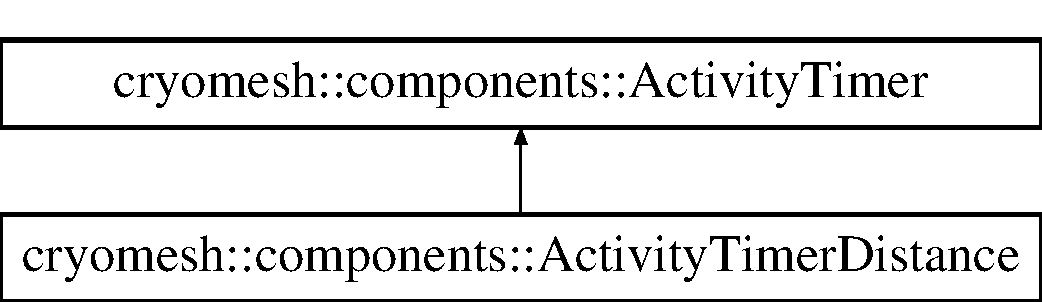
\includegraphics[height=2.000000cm]{classcryomesh_1_1components_1_1ActivityTimer}
\end{center}
\end{figure}
\subsection*{\-Public \-Member \-Functions}
\begin{DoxyCompactItemize}
\item 
\hyperlink{classcryomesh_1_1components_1_1ActivityTimer_abf1241a780f7c6fa5d626b4585afc017}{\-Activity\-Timer} ()
\begin{DoxyCompactList}\small\item\em \-Default constructor. \end{DoxyCompactList}\item 
virtual \hyperlink{classcryomesh_1_1components_1_1ActivityTimer_a8383004d633ae75433d3961bdec431cf}{$\sim$\-Activity\-Timer} ()
\begin{DoxyCompactList}\small\item\em \-Default destructor. \end{DoxyCompactList}\item 
virtual void \hyperlink{classcryomesh_1_1components_1_1ActivityTimer_a8842b0b6e73ddf1d1809b79b7b239baf}{reset} ()=0
\end{DoxyCompactItemize}
\subsection*{\-Protected \-Member \-Functions}
\begin{DoxyCompactItemize}
\item 
virtual std\-::ostream \& \hyperlink{classcryomesh_1_1components_1_1ActivityTimer_a1a4fd82c20fdc2b17ebe4582222ab8a3}{print} (std\-::ostream \&os) const =0
\end{DoxyCompactItemize}
\subsection*{\-Friends}
\begin{DoxyCompactItemize}
\item 
std\-::ostream \& \hyperlink{classcryomesh_1_1components_1_1ActivityTimer_ac35779cd02eec3662a6cd9d75e1572cd}{operator$<$$<$} (std\-::ostream \&os, const \hyperlink{classcryomesh_1_1components_1_1ActivityTimer}{\-Activity\-Timer} \&obj)
\begin{DoxyCompactList}\small\item\em \-To stream operator. \end{DoxyCompactList}\end{DoxyCompactItemize}


\subsection{\-Detailed \-Description}
\-Simple interface class for activity timers. 

\-Definition at line 20 of file \-Activity\-Timer.\-h.



\subsection{\-Constructor \& \-Destructor \-Documentation}
\hypertarget{classcryomesh_1_1components_1_1ActivityTimer_abf1241a780f7c6fa5d626b4585afc017}{\index{cryomesh\-::components\-::\-Activity\-Timer@{cryomesh\-::components\-::\-Activity\-Timer}!\-Activity\-Timer@{\-Activity\-Timer}}
\index{\-Activity\-Timer@{\-Activity\-Timer}!cryomesh::components::ActivityTimer@{cryomesh\-::components\-::\-Activity\-Timer}}
\subsubsection[{\-Activity\-Timer}]{\setlength{\rightskip}{0pt plus 5cm}{\bf cryomesh\-::components\-::\-Activity\-Timer\-::\-Activity\-Timer} (
\begin{DoxyParamCaption}
{}
\end{DoxyParamCaption}
)\hspace{0.3cm}{\ttfamily  \mbox{[}inline\mbox{]}}}}\label{classcryomesh_1_1components_1_1ActivityTimer_abf1241a780f7c6fa5d626b4585afc017}


\-Default constructor. 



\-Definition at line 25 of file \-Activity\-Timer.\-h.

\hypertarget{classcryomesh_1_1components_1_1ActivityTimer_a8383004d633ae75433d3961bdec431cf}{\index{cryomesh\-::components\-::\-Activity\-Timer@{cryomesh\-::components\-::\-Activity\-Timer}!$\sim$\-Activity\-Timer@{$\sim$\-Activity\-Timer}}
\index{$\sim$\-Activity\-Timer@{$\sim$\-Activity\-Timer}!cryomesh::components::ActivityTimer@{cryomesh\-::components\-::\-Activity\-Timer}}
\subsubsection[{$\sim$\-Activity\-Timer}]{\setlength{\rightskip}{0pt plus 5cm}virtual {\bf cryomesh\-::components\-::\-Activity\-Timer\-::$\sim$\-Activity\-Timer} (
\begin{DoxyParamCaption}
{}
\end{DoxyParamCaption}
)\hspace{0.3cm}{\ttfamily  \mbox{[}inline, virtual\mbox{]}}}}\label{classcryomesh_1_1components_1_1ActivityTimer_a8383004d633ae75433d3961bdec431cf}


\-Default destructor. 



\-Definition at line 31 of file \-Activity\-Timer.\-h.



\subsection{\-Member \-Function \-Documentation}
\hypertarget{classcryomesh_1_1components_1_1ActivityTimer_a1a4fd82c20fdc2b17ebe4582222ab8a3}{\index{cryomesh\-::components\-::\-Activity\-Timer@{cryomesh\-::components\-::\-Activity\-Timer}!print@{print}}
\index{print@{print}!cryomesh::components::ActivityTimer@{cryomesh\-::components\-::\-Activity\-Timer}}
\subsubsection[{print}]{\setlength{\rightskip}{0pt plus 5cm}virtual std\-::ostream\& {\bf cryomesh\-::components\-::\-Activity\-Timer\-::print} (
\begin{DoxyParamCaption}
\item[{std\-::ostream \&}]{os}
\end{DoxyParamCaption}
) const\hspace{0.3cm}{\ttfamily  \mbox{[}protected, pure virtual\mbox{]}}}}\label{classcryomesh_1_1components_1_1ActivityTimer_a1a4fd82c20fdc2b17ebe4582222ab8a3}


\-Implemented in \hyperlink{classcryomesh_1_1components_1_1ActivityTimerDistance_a6e109b8f4ddcf6d4e24f0347d4060f78}{cryomesh\-::components\-::\-Activity\-Timer\-Distance}.

\hypertarget{classcryomesh_1_1components_1_1ActivityTimer_a8842b0b6e73ddf1d1809b79b7b239baf}{\index{cryomesh\-::components\-::\-Activity\-Timer@{cryomesh\-::components\-::\-Activity\-Timer}!reset@{reset}}
\index{reset@{reset}!cryomesh::components::ActivityTimer@{cryomesh\-::components\-::\-Activity\-Timer}}
\subsubsection[{reset}]{\setlength{\rightskip}{0pt plus 5cm}virtual void {\bf cryomesh\-::components\-::\-Activity\-Timer\-::reset} (
\begin{DoxyParamCaption}
{}
\end{DoxyParamCaption}
)\hspace{0.3cm}{\ttfamily  \mbox{[}pure virtual\mbox{]}}}}\label{classcryomesh_1_1components_1_1ActivityTimer_a8842b0b6e73ddf1d1809b79b7b239baf}


\-Implemented in \hyperlink{classcryomesh_1_1components_1_1ActivityTimerDistance_aca048029f8ff311c7e215bb2d7689c7b}{cryomesh\-::components\-::\-Activity\-Timer\-Distance}.



\subsection{\-Friends \-And \-Related \-Function \-Documentation}
\hypertarget{classcryomesh_1_1components_1_1ActivityTimer_ac35779cd02eec3662a6cd9d75e1572cd}{\index{cryomesh\-::components\-::\-Activity\-Timer@{cryomesh\-::components\-::\-Activity\-Timer}!operator$<$$<$@{operator$<$$<$}}
\index{operator$<$$<$@{operator$<$$<$}!cryomesh::components::ActivityTimer@{cryomesh\-::components\-::\-Activity\-Timer}}
\subsubsection[{operator$<$$<$}]{\setlength{\rightskip}{0pt plus 5cm}std\-::ostream\& operator$<$$<$ (
\begin{DoxyParamCaption}
\item[{std\-::ostream \&}]{os, }
\item[{const {\bf \-Activity\-Timer} \&}]{obj}
\end{DoxyParamCaption}
)\hspace{0.3cm}{\ttfamily  \mbox{[}friend\mbox{]}}}}\label{classcryomesh_1_1components_1_1ActivityTimer_ac35779cd02eec3662a6cd9d75e1572cd}


\-To stream operator. 


\begin{DoxyParams}{\-Parameters}
{\em std\-::ostream} & \& os \-The output stream \\
\hline
{\em const} & \hyperlink{classcryomesh_1_1components_1_1ActivityTimer}{\-Activity\-Timer} \& obj \-The object to stream\\
\hline
\end{DoxyParams}
\begin{DoxyReturn}{\-Returns}
std\-::ostream \& \-The output stream 
\end{DoxyReturn}


\-Definition at line 47 of file \-Activity\-Timer.\-h.



\-The documentation for this class was generated from the following file\-:\begin{DoxyCompactItemize}
\item 
/home/niall/\-Projects/\-Eclipse/\-C\-P\-P/cryomesh/src/components/\hyperlink{ActivityTimer_8h}{\-Activity\-Timer.\-h}\end{DoxyCompactItemize}

\hypertarget{classcryomesh_1_1components_1_1ActivityTimerDistance}{\section{cryomesh\-:\-:components\-:\-:\-Activity\-Timer\-Distance \-Class \-Reference}
\label{classcryomesh_1_1components_1_1ActivityTimerDistance}\index{cryomesh\-::components\-::\-Activity\-Timer\-Distance@{cryomesh\-::components\-::\-Activity\-Timer\-Distance}}
}


{\ttfamily \#include $<$\-Activity\-Timer\-Distance.\-h$>$}

\-Inheritance diagram for cryomesh\-:\-:components\-:\-:\-Activity\-Timer\-Distance\-:\begin{figure}[H]
\begin{center}
\leavevmode
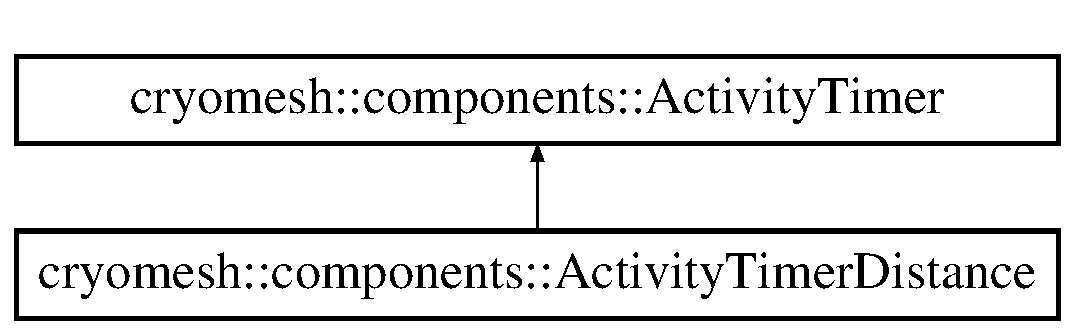
\includegraphics[height=2.000000cm]{classcryomesh_1_1components_1_1ActivityTimerDistance}
\end{center}
\end{figure}
\subsection*{\-Public \-Member \-Functions}
\begin{DoxyCompactItemize}
\item 
\hyperlink{classcryomesh_1_1components_1_1ActivityTimerDistance_a3da36944fccd3512740a63fdae13de20}{\-Activity\-Timer\-Distance} ()
\begin{DoxyCompactList}\small\item\em \-Constructor. \end{DoxyCompactList}\item 
\hyperlink{classcryomesh_1_1components_1_1ActivityTimerDistance_a09f1241cc4c1ddd4423ac288e534b1e1}{\-Activity\-Timer\-Distance} (double dist, double dec)
\begin{DoxyCompactList}\small\item\em \-Construct from an initial distance, and a rate of decrement. \end{DoxyCompactList}\item 
virtual \hyperlink{classcryomesh_1_1components_1_1ActivityTimerDistance_ac31091719dbdcebb505a47a2ed99fc4e}{$\sim$\-Activity\-Timer\-Distance} ()
\item 
\hyperlink{classcryomesh_1_1components_1_1ActivityTimerDistance}{\-Activity\-Timer\-Distance} \& \hyperlink{classcryomesh_1_1components_1_1ActivityTimerDistance_a37992cab5a1bfde00c8f069fc47a7c2f}{operator=} (const \hyperlink{classcryomesh_1_1components_1_1ActivityTimerDistance}{\-Activity\-Timer\-Distance} \&obj)
\begin{DoxyCompactList}\small\item\em \-Assignment operator. \end{DoxyCompactList}\item 
bool \hyperlink{classcryomesh_1_1components_1_1ActivityTimerDistance_a36db36aad72526f4d1541213ed762c01}{operator$<$} (const \hyperlink{classcryomesh_1_1components_1_1ActivityTimerDistance}{\-Activity\-Timer\-Distance} \&obj) const 
\begin{DoxyCompactList}\small\item\em \-Less than operator. \end{DoxyCompactList}\item 
bool \hyperlink{classcryomesh_1_1components_1_1ActivityTimerDistance_ae33ecef3ba181aec976ceb6304fc7935}{operator$>$} (const \hyperlink{classcryomesh_1_1components_1_1ActivityTimerDistance}{\-Activity\-Timer\-Distance} \&obj) const 
\begin{DoxyCompactList}\small\item\em \-Greater than operator. \end{DoxyCompactList}\item 
\hyperlink{classcryomesh_1_1components_1_1ActivityTimerDistance}{\-Activity\-Timer\-Distance} \& \hyperlink{classcryomesh_1_1components_1_1ActivityTimerDistance_adf508add943655664c792c93795406fd}{operator-\/-\/} ()
\begin{DoxyCompactList}\small\item\em \-Prefix increment operator. \end{DoxyCompactList}\item 
\hyperlink{classcryomesh_1_1components_1_1ActivityTimerDistance}{\-Activity\-Timer\-Distance} \hyperlink{classcryomesh_1_1components_1_1ActivityTimerDistance_aa8f2cf4dbabcc623aa7e0cf1f793f98a}{operator-\/-\/} (int)
\begin{DoxyCompactList}\small\item\em \-Postfix decrement operator. \end{DoxyCompactList}\item 
const \hyperlink{classcryomesh_1_1components_1_1ActivityTimerDistance}{\-Activity\-Timer\-Distance} \hyperlink{classcryomesh_1_1components_1_1ActivityTimerDistance_a7c91c5d5255899d6504cc3fe6669cbab}{operator+} (const \hyperlink{classcryomesh_1_1components_1_1ActivityTimerDistance}{\-Activity\-Timer\-Distance} \&obj) const 
\begin{DoxyCompactList}\small\item\em \-Non-\/destructive addition operator. \end{DoxyCompactList}\item 
\hyperlink{classcryomesh_1_1components_1_1ActivityTimerDistance}{\-Activity\-Timer\-Distance} \& \hyperlink{classcryomesh_1_1components_1_1ActivityTimerDistance_aaf72572d1cb481f519132e7a17b8125b}{operator+=} (const \hyperlink{classcryomesh_1_1components_1_1ActivityTimerDistance}{\-Activity\-Timer\-Distance} \&obj)
\begin{DoxyCompactList}\small\item\em \-Destructive addition and assignment operator. \end{DoxyCompactList}\item 
double \hyperlink{classcryomesh_1_1components_1_1ActivityTimerDistance_aa0ded366836ca5bb7ce9db6abf7b4d51}{get\-Delay} () const 
\begin{DoxyCompactList}\small\item\em \-Get the delay. \end{DoxyCompactList}\item 
double \hyperlink{classcryomesh_1_1components_1_1ActivityTimerDistance_a7da9fc6bc83657837f90ad3a6158e3a5}{get\-Starting\-Delay} () const 
\begin{DoxyCompactList}\small\item\em \-Get the starting delay. \end{DoxyCompactList}\item 
double \hyperlink{classcryomesh_1_1components_1_1ActivityTimerDistance_a3691132699928dc9f7089576ad0c12ce}{get\-Decrement} () const 
\begin{DoxyCompactList}\small\item\em \-Get the decrement. \end{DoxyCompactList}\item 
void \hyperlink{classcryomesh_1_1components_1_1ActivityTimerDistance_aca048029f8ff311c7e215bb2d7689c7b}{reset} ()
\begin{DoxyCompactList}\small\item\em \-Reset the countdown. \end{DoxyCompactList}\item 
virtual bool \hyperlink{classcryomesh_1_1components_1_1ActivityTimerDistance_a2e2ac1b8bc8d942346c1a758d7602a99}{check\-Constraints} () const 
\item 
virtual void \hyperlink{classcryomesh_1_1components_1_1ActivityTimerDistance_a54d73b877fd99ece736c7352a09688ad}{enable\-Debug} (bool b)
\end{DoxyCompactItemize}
\subsection*{\-Static \-Public \-Member \-Functions}
\begin{DoxyCompactItemize}
\item 
static boost\-::shared\-\_\-ptr\*
$<$ \hyperlink{classcryomesh_1_1components_1_1ActivityTimerDistance}{\-Activity\-Timer\-Distance} $>$ \hyperlink{classcryomesh_1_1components_1_1ActivityTimerDistance_ad82f62afe5a34af54ff4c4ec8d1c2344}{get\-Random} ()
\begin{DoxyCompactList}\small\item\em \-Get a random object. \end{DoxyCompactList}\end{DoxyCompactItemize}
\subsection*{\-Static \-Public \-Attributes}
\begin{DoxyCompactItemize}
\item 
static const double \hyperlink{classcryomesh_1_1components_1_1ActivityTimerDistance_afb9cf33e702747ecd42d1bfd0c3a3ce3}{\-M\-I\-N\-\_\-\-D\-E\-C\-R\-E\-M\-E\-N\-T\-\_\-\-F\-R\-A\-C\-T\-I\-O\-N} = 0.\-1
\item 
static const double \hyperlink{classcryomesh_1_1components_1_1ActivityTimerDistance_ab24df04f889693641f609aa8f199455f}{\-M\-A\-X\-\_\-\-D\-E\-C\-R\-E\-M\-E\-N\-T\-\_\-\-F\-R\-A\-C\-T\-I\-O\-N} = 1
\item 
static const double \hyperlink{classcryomesh_1_1components_1_1ActivityTimerDistance_a549f2e016df32a594092179570ae742d}{\-M\-I\-N\-\_\-\-D\-I\-S\-T\-A\-N\-C\-E} = 1.\-0
\item 
static const double \hyperlink{classcryomesh_1_1components_1_1ActivityTimerDistance_a87e36fd0ad252132017fa1c9664cf2ca}{\-M\-A\-X\-\_\-\-D\-I\-S\-T\-A\-N\-C\-E} = 100.\-0
\end{DoxyCompactItemize}
\subsection*{\-Protected \-Member \-Functions}
\begin{DoxyCompactItemize}
\item 
virtual std\-::ostream \& \hyperlink{classcryomesh_1_1components_1_1ActivityTimerDistance_a6e109b8f4ddcf6d4e24f0347d4060f78}{print} (std\-::ostream \&os) const 
\end{DoxyCompactItemize}
\subsection*{\-Private \-Attributes}
\begin{DoxyCompactItemize}
\item 
double \hyperlink{classcryomesh_1_1components_1_1ActivityTimerDistance_a191b202e783b14973aa327c460cdc46e}{distance}
\item 
double \hyperlink{classcryomesh_1_1components_1_1ActivityTimerDistance_a0e793c735a10edd18fa12a019dcf8c22}{distance\-\_\-remaining}
\item 
double \hyperlink{classcryomesh_1_1components_1_1ActivityTimerDistance_a81f6c8dffa1dbe89e7e3d67603f84b9a}{decrement}
\end{DoxyCompactItemize}
\subsection*{\-Friends}
\begin{DoxyCompactItemize}
\item 
std\-::ostream \& \hyperlink{classcryomesh_1_1components_1_1ActivityTimer_ac35779cd02eec3662a6cd9d75e1572cd}{operator$<$$<$} (std\-::ostream \&os, const \hyperlink{classcryomesh_1_1components_1_1ActivityTimer}{\-Activity\-Timer} \&obj)
\begin{DoxyCompactList}\small\item\em \-To stream operator. \end{DoxyCompactList}\end{DoxyCompactItemize}


\subsection{\-Detailed \-Description}


\-Definition at line 19 of file \-Activity\-Timer\-Distance.\-h.



\subsection{\-Constructor \& \-Destructor \-Documentation}
\hypertarget{classcryomesh_1_1components_1_1ActivityTimerDistance_a3da36944fccd3512740a63fdae13de20}{\index{cryomesh\-::components\-::\-Activity\-Timer\-Distance@{cryomesh\-::components\-::\-Activity\-Timer\-Distance}!\-Activity\-Timer\-Distance@{\-Activity\-Timer\-Distance}}
\index{\-Activity\-Timer\-Distance@{\-Activity\-Timer\-Distance}!cryomesh::components::ActivityTimerDistance@{cryomesh\-::components\-::\-Activity\-Timer\-Distance}}
\subsubsection[{\-Activity\-Timer\-Distance}]{\setlength{\rightskip}{0pt plus 5cm}{\bf cryomesh\-::components\-::\-Activity\-Timer\-Distance\-::\-Activity\-Timer\-Distance} (
\begin{DoxyParamCaption}
{}
\end{DoxyParamCaption}
)}}\label{classcryomesh_1_1components_1_1ActivityTimerDistance_a3da36944fccd3512740a63fdae13de20}


\-Constructor. 



\-Definition at line 36 of file \-Activity\-Timer\-Distance.\-cpp.



\-Referenced by get\-Random().

\hypertarget{classcryomesh_1_1components_1_1ActivityTimerDistance_a09f1241cc4c1ddd4423ac288e534b1e1}{\index{cryomesh\-::components\-::\-Activity\-Timer\-Distance@{cryomesh\-::components\-::\-Activity\-Timer\-Distance}!\-Activity\-Timer\-Distance@{\-Activity\-Timer\-Distance}}
\index{\-Activity\-Timer\-Distance@{\-Activity\-Timer\-Distance}!cryomesh::components::ActivityTimerDistance@{cryomesh\-::components\-::\-Activity\-Timer\-Distance}}
\subsubsection[{\-Activity\-Timer\-Distance}]{\setlength{\rightskip}{0pt plus 5cm}{\bf cryomesh\-::components\-::\-Activity\-Timer\-Distance\-::\-Activity\-Timer\-Distance} (
\begin{DoxyParamCaption}
\item[{double}]{dist, }
\item[{double}]{dec}
\end{DoxyParamCaption}
)}}\label{classcryomesh_1_1components_1_1ActivityTimerDistance_a09f1241cc4c1ddd4423ac288e534b1e1}


\-Construct from an initial distance, and a rate of decrement. 



\-Definition at line 40 of file \-Activity\-Timer\-Distance.\-cpp.

\hypertarget{classcryomesh_1_1components_1_1ActivityTimerDistance_ac31091719dbdcebb505a47a2ed99fc4e}{\index{cryomesh\-::components\-::\-Activity\-Timer\-Distance@{cryomesh\-::components\-::\-Activity\-Timer\-Distance}!$\sim$\-Activity\-Timer\-Distance@{$\sim$\-Activity\-Timer\-Distance}}
\index{$\sim$\-Activity\-Timer\-Distance@{$\sim$\-Activity\-Timer\-Distance}!cryomesh::components::ActivityTimerDistance@{cryomesh\-::components\-::\-Activity\-Timer\-Distance}}
\subsubsection[{$\sim$\-Activity\-Timer\-Distance}]{\setlength{\rightskip}{0pt plus 5cm}{\bf cryomesh\-::components\-::\-Activity\-Timer\-Distance\-::$\sim$\-Activity\-Timer\-Distance} (
\begin{DoxyParamCaption}
{}
\end{DoxyParamCaption}
)\hspace{0.3cm}{\ttfamily  \mbox{[}virtual\mbox{]}}}}\label{classcryomesh_1_1components_1_1ActivityTimerDistance_ac31091719dbdcebb505a47a2ed99fc4e}


\-Definition at line 44 of file \-Activity\-Timer\-Distance.\-cpp.



\subsection{\-Member \-Function \-Documentation}
\hypertarget{classcryomesh_1_1components_1_1ActivityTimerDistance_a2e2ac1b8bc8d942346c1a758d7602a99}{\index{cryomesh\-::components\-::\-Activity\-Timer\-Distance@{cryomesh\-::components\-::\-Activity\-Timer\-Distance}!check\-Constraints@{check\-Constraints}}
\index{check\-Constraints@{check\-Constraints}!cryomesh::components::ActivityTimerDistance@{cryomesh\-::components\-::\-Activity\-Timer\-Distance}}
\subsubsection[{check\-Constraints}]{\setlength{\rightskip}{0pt plus 5cm}bool {\bf cryomesh\-::components\-::\-Activity\-Timer\-Distance\-::check\-Constraints} (
\begin{DoxyParamCaption}
{}
\end{DoxyParamCaption}
) const\hspace{0.3cm}{\ttfamily  \mbox{[}virtual\mbox{]}}}}\label{classcryomesh_1_1components_1_1ActivityTimerDistance_a2e2ac1b8bc8d942346c1a758d7602a99}


\-Definition at line 113 of file \-Activity\-Timer\-Distance.\-cpp.



\-References get\-Decrement(), get\-Starting\-Delay(), and \-M\-I\-N\-\_\-\-D\-I\-S\-T\-A\-N\-C\-E.

\hypertarget{classcryomesh_1_1components_1_1ActivityTimerDistance_a54d73b877fd99ece736c7352a09688ad}{\index{cryomesh\-::components\-::\-Activity\-Timer\-Distance@{cryomesh\-::components\-::\-Activity\-Timer\-Distance}!enable\-Debug@{enable\-Debug}}
\index{enable\-Debug@{enable\-Debug}!cryomesh::components::ActivityTimerDistance@{cryomesh\-::components\-::\-Activity\-Timer\-Distance}}
\subsubsection[{enable\-Debug}]{\setlength{\rightskip}{0pt plus 5cm}void {\bf cryomesh\-::components\-::\-Activity\-Timer\-Distance\-::enable\-Debug} (
\begin{DoxyParamCaption}
\item[{bool}]{b}
\end{DoxyParamCaption}
)\hspace{0.3cm}{\ttfamily  \mbox{[}virtual\mbox{]}}}}\label{classcryomesh_1_1components_1_1ActivityTimerDistance_a54d73b877fd99ece736c7352a09688ad}


\-Definition at line 101 of file \-Activity\-Timer\-Distance.\-cpp.

\hypertarget{classcryomesh_1_1components_1_1ActivityTimerDistance_a3691132699928dc9f7089576ad0c12ce}{\index{cryomesh\-::components\-::\-Activity\-Timer\-Distance@{cryomesh\-::components\-::\-Activity\-Timer\-Distance}!get\-Decrement@{get\-Decrement}}
\index{get\-Decrement@{get\-Decrement}!cryomesh::components::ActivityTimerDistance@{cryomesh\-::components\-::\-Activity\-Timer\-Distance}}
\subsubsection[{get\-Decrement}]{\setlength{\rightskip}{0pt plus 5cm}double {\bf cryomesh\-::components\-::\-Activity\-Timer\-Distance\-::get\-Decrement} (
\begin{DoxyParamCaption}
{}
\end{DoxyParamCaption}
) const}}\label{classcryomesh_1_1components_1_1ActivityTimerDistance_a3691132699928dc9f7089576ad0c12ce}


\-Get the decrement. 

\begin{DoxyReturn}{\-Returns}
double \-The decrement of the timer 
\end{DoxyReturn}


\-Definition at line 98 of file \-Activity\-Timer\-Distance.\-cpp.



\-References decrement.



\-Referenced by check\-Constraints(), and print().

\hypertarget{classcryomesh_1_1components_1_1ActivityTimerDistance_aa0ded366836ca5bb7ce9db6abf7b4d51}{\index{cryomesh\-::components\-::\-Activity\-Timer\-Distance@{cryomesh\-::components\-::\-Activity\-Timer\-Distance}!get\-Delay@{get\-Delay}}
\index{get\-Delay@{get\-Delay}!cryomesh::components::ActivityTimerDistance@{cryomesh\-::components\-::\-Activity\-Timer\-Distance}}
\subsubsection[{get\-Delay}]{\setlength{\rightskip}{0pt plus 5cm}double {\bf cryomesh\-::components\-::\-Activity\-Timer\-Distance\-::get\-Delay} (
\begin{DoxyParamCaption}
{}
\end{DoxyParamCaption}
) const}}\label{classcryomesh_1_1components_1_1ActivityTimerDistance_aa0ded366836ca5bb7ce9db6abf7b4d51}


\-Get the delay. 

\begin{DoxyReturn}{\-Returns}
double \-The distance delay 
\end{DoxyReturn}


\-Definition at line 90 of file \-Activity\-Timer\-Distance.\-cpp.



\-References distance\-\_\-remaining.



\-Referenced by print().

\hypertarget{classcryomesh_1_1components_1_1ActivityTimerDistance_ad82f62afe5a34af54ff4c4ec8d1c2344}{\index{cryomesh\-::components\-::\-Activity\-Timer\-Distance@{cryomesh\-::components\-::\-Activity\-Timer\-Distance}!get\-Random@{get\-Random}}
\index{get\-Random@{get\-Random}!cryomesh::components::ActivityTimerDistance@{cryomesh\-::components\-::\-Activity\-Timer\-Distance}}
\subsubsection[{get\-Random}]{\setlength{\rightskip}{0pt plus 5cm}boost\-::shared\-\_\-ptr$<$ {\bf \-Activity\-Timer\-Distance} $>$ {\bf cryomesh\-::components\-::\-Activity\-Timer\-Distance\-::get\-Random} (
\begin{DoxyParamCaption}
{}
\end{DoxyParamCaption}
)\hspace{0.3cm}{\ttfamily  \mbox{[}static\mbox{]}}}}\label{classcryomesh_1_1components_1_1ActivityTimerDistance_ad82f62afe5a34af54ff4c4ec8d1c2344}


\-Get a random object. 

\begin{DoxyReturn}{\-Returns}
boost\-::shared\-\_\-ptr$<$\-Activity\-Timer\-Distance$>$ \-The random object 
\end{DoxyReturn}


\-Definition at line 22 of file \-Activity\-Timer\-Distance.\-cpp.



\-References \-Activity\-Timer\-Distance(), \-M\-A\-X\-\_\-\-D\-E\-C\-R\-E\-M\-E\-N\-T\-\_\-\-F\-R\-A\-C\-T\-I\-O\-N, \-M\-A\-X\-\_\-\-D\-I\-S\-T\-A\-N\-C\-E, \-M\-I\-N\-\_\-\-D\-E\-C\-R\-E\-M\-E\-N\-T\-\_\-\-F\-R\-A\-C\-T\-I\-O\-N, and \-M\-I\-N\-\_\-\-D\-I\-S\-T\-A\-N\-C\-E.

\hypertarget{classcryomesh_1_1components_1_1ActivityTimerDistance_a7da9fc6bc83657837f90ad3a6158e3a5}{\index{cryomesh\-::components\-::\-Activity\-Timer\-Distance@{cryomesh\-::components\-::\-Activity\-Timer\-Distance}!get\-Starting\-Delay@{get\-Starting\-Delay}}
\index{get\-Starting\-Delay@{get\-Starting\-Delay}!cryomesh::components::ActivityTimerDistance@{cryomesh\-::components\-::\-Activity\-Timer\-Distance}}
\subsubsection[{get\-Starting\-Delay}]{\setlength{\rightskip}{0pt plus 5cm}double {\bf cryomesh\-::components\-::\-Activity\-Timer\-Distance\-::get\-Starting\-Delay} (
\begin{DoxyParamCaption}
{}
\end{DoxyParamCaption}
) const}}\label{classcryomesh_1_1components_1_1ActivityTimerDistance_a7da9fc6bc83657837f90ad3a6158e3a5}


\-Get the starting delay. 

\begin{DoxyReturn}{\-Returns}
double \-The starting distance delay 
\end{DoxyReturn}


\-Definition at line 94 of file \-Activity\-Timer\-Distance.\-cpp.



\-References distance.



\-Referenced by check\-Constraints(), and print().

\hypertarget{classcryomesh_1_1components_1_1ActivityTimerDistance_a7c91c5d5255899d6504cc3fe6669cbab}{\index{cryomesh\-::components\-::\-Activity\-Timer\-Distance@{cryomesh\-::components\-::\-Activity\-Timer\-Distance}!operator+@{operator+}}
\index{operator+@{operator+}!cryomesh::components::ActivityTimerDistance@{cryomesh\-::components\-::\-Activity\-Timer\-Distance}}
\subsubsection[{operator+}]{\setlength{\rightskip}{0pt plus 5cm}const {\bf \-Activity\-Timer\-Distance} cryomesh\-::components\-::\-Activity\-Timer\-Distance\-::operator+ (
\begin{DoxyParamCaption}
\item[{const {\bf \-Activity\-Timer\-Distance} \&}]{obj}
\end{DoxyParamCaption}
) const}}\label{classcryomesh_1_1components_1_1ActivityTimerDistance_a7c91c5d5255899d6504cc3fe6669cbab}


\-Non-\/destructive addition operator. 


\begin{DoxyParams}{\-Parameters}
{\em const} & \hyperlink{classcryomesh_1_1components_1_1ActivityTimerDistance}{\-Activity\-Timer\-Distance} \& obj \-R\-H\-S addition\\
\hline
\end{DoxyParams}
\begin{DoxyReturn}{\-Returns}
\hyperlink{classcryomesh_1_1components_1_1ActivityTimerDistance}{\-Activity\-Timer\-Distance} \-New object after addition 
\end{DoxyReturn}


\-Definition at line 76 of file \-Activity\-Timer\-Distance.\-cpp.

\hypertarget{classcryomesh_1_1components_1_1ActivityTimerDistance_aaf72572d1cb481f519132e7a17b8125b}{\index{cryomesh\-::components\-::\-Activity\-Timer\-Distance@{cryomesh\-::components\-::\-Activity\-Timer\-Distance}!operator+=@{operator+=}}
\index{operator+=@{operator+=}!cryomesh::components::ActivityTimerDistance@{cryomesh\-::components\-::\-Activity\-Timer\-Distance}}
\subsubsection[{operator+=}]{\setlength{\rightskip}{0pt plus 5cm}{\bf \-Activity\-Timer\-Distance} \& cryomesh\-::components\-::\-Activity\-Timer\-Distance\-::operator+= (
\begin{DoxyParamCaption}
\item[{const {\bf \-Activity\-Timer\-Distance} \&}]{obj}
\end{DoxyParamCaption}
)}}\label{classcryomesh_1_1components_1_1ActivityTimerDistance_aaf72572d1cb481f519132e7a17b8125b}


\-Destructive addition and assignment operator. 


\begin{DoxyParams}{\-Parameters}
{\em const} & \hyperlink{classcryomesh_1_1components_1_1ActivityTimerDistance}{\-Activity\-Timer\-Distance} \& obj \-R\-H\-S addition\\
\hline
\end{DoxyParams}
\begin{DoxyReturn}{\-Returns}
\hyperlink{classcryomesh_1_1components_1_1ActivityTimerDistance}{\-Activity\-Timer\-Distance} \& \-This object after addition and assignment 
\end{DoxyReturn}


\-Definition at line 82 of file \-Activity\-Timer\-Distance.\-cpp.



\-References decrement, distance, and distance\-\_\-remaining.

\hypertarget{classcryomesh_1_1components_1_1ActivityTimerDistance_adf508add943655664c792c93795406fd}{\index{cryomesh\-::components\-::\-Activity\-Timer\-Distance@{cryomesh\-::components\-::\-Activity\-Timer\-Distance}!operator-\/-\/@{operator-\/-\/}}
\index{operator-\/-\/@{operator-\/-\/}!cryomesh::components::ActivityTimerDistance@{cryomesh\-::components\-::\-Activity\-Timer\-Distance}}
\subsubsection[{operator-\/-\/}]{\setlength{\rightskip}{0pt plus 5cm}{\bf \-Activity\-Timer\-Distance} \& cryomesh\-::components\-::\-Activity\-Timer\-Distance\-::operator-\/-\/ (
\begin{DoxyParamCaption}
{}
\end{DoxyParamCaption}
)}}\label{classcryomesh_1_1components_1_1ActivityTimerDistance_adf508add943655664c792c93795406fd}


\-Prefix increment operator. 

\begin{DoxyReturn}{\-Returns}
\hyperlink{classcryomesh_1_1components_1_1ActivityTimerDistance}{\-Activity\-Timer\-Distance} \& \-Return this 
\end{DoxyReturn}


\-Definition at line 62 of file \-Activity\-Timer\-Distance.\-cpp.



\-References decrement, and distance\-\_\-remaining.

\hypertarget{classcryomesh_1_1components_1_1ActivityTimerDistance_aa8f2cf4dbabcc623aa7e0cf1f793f98a}{\index{cryomesh\-::components\-::\-Activity\-Timer\-Distance@{cryomesh\-::components\-::\-Activity\-Timer\-Distance}!operator-\/-\/@{operator-\/-\/}}
\index{operator-\/-\/@{operator-\/-\/}!cryomesh::components::ActivityTimerDistance@{cryomesh\-::components\-::\-Activity\-Timer\-Distance}}
\subsubsection[{operator-\/-\/}]{\setlength{\rightskip}{0pt plus 5cm}{\bf \-Activity\-Timer\-Distance} cryomesh\-::components\-::\-Activity\-Timer\-Distance\-::operator-\/-\/ (
\begin{DoxyParamCaption}
\item[{int}]{}
\end{DoxyParamCaption}
)}}\label{classcryomesh_1_1components_1_1ActivityTimerDistance_aa8f2cf4dbabcc623aa7e0cf1f793f98a}


\-Postfix decrement operator. 

\begin{DoxyReturn}{\-Returns}
\hyperlink{classcryomesh_1_1components_1_1ActivityTimerDistance}{\-Activity\-Timer\-Distance} \& \-Return this 
\end{DoxyReturn}


\-Definition at line 70 of file \-Activity\-Timer\-Distance.\-cpp.

\hypertarget{classcryomesh_1_1components_1_1ActivityTimerDistance_a36db36aad72526f4d1541213ed762c01}{\index{cryomesh\-::components\-::\-Activity\-Timer\-Distance@{cryomesh\-::components\-::\-Activity\-Timer\-Distance}!operator$<$@{operator$<$}}
\index{operator$<$@{operator$<$}!cryomesh::components::ActivityTimerDistance@{cryomesh\-::components\-::\-Activity\-Timer\-Distance}}
\subsubsection[{operator$<$}]{\setlength{\rightskip}{0pt plus 5cm}bool cryomesh\-::components\-::\-Activity\-Timer\-Distance\-::operator$<$ (
\begin{DoxyParamCaption}
\item[{const {\bf \-Activity\-Timer\-Distance} \&}]{obj}
\end{DoxyParamCaption}
) const}}\label{classcryomesh_1_1components_1_1ActivityTimerDistance_a36db36aad72526f4d1541213ed762c01}


\-Less than operator. 


\begin{DoxyParams}{\-Parameters}
{\em const} & \hyperlink{classcryomesh_1_1components_1_1ActivityTimerDistance}{\-Activity\-Timer\-Distance} \& obj \-R\-H\-S\\
\hline
\end{DoxyParams}
\begin{DoxyReturn}{\-Returns}
bool \-True if $<$ than obj, false otherwise 
\end{DoxyReturn}


\-Definition at line 54 of file \-Activity\-Timer\-Distance.\-cpp.



\-References distance.

\hypertarget{classcryomesh_1_1components_1_1ActivityTimerDistance_a37992cab5a1bfde00c8f069fc47a7c2f}{\index{cryomesh\-::components\-::\-Activity\-Timer\-Distance@{cryomesh\-::components\-::\-Activity\-Timer\-Distance}!operator=@{operator=}}
\index{operator=@{operator=}!cryomesh::components::ActivityTimerDistance@{cryomesh\-::components\-::\-Activity\-Timer\-Distance}}
\subsubsection[{operator=}]{\setlength{\rightskip}{0pt plus 5cm}{\bf \-Activity\-Timer\-Distance} \& cryomesh\-::components\-::\-Activity\-Timer\-Distance\-::operator= (
\begin{DoxyParamCaption}
\item[{const {\bf \-Activity\-Timer\-Distance} \&}]{obj}
\end{DoxyParamCaption}
)}}\label{classcryomesh_1_1components_1_1ActivityTimerDistance_a37992cab5a1bfde00c8f069fc47a7c2f}


\-Assignment operator. 


\begin{DoxyParams}{\-Parameters}
{\em const} & \hyperlink{classcryomesh_1_1components_1_1ActivityTimerDistance}{\-Activity\-Timer\-Distance} \& obj \-R\-H\-S assignment\\
\hline
\end{DoxyParams}
\begin{DoxyReturn}{\-Returns}
\hyperlink{classcryomesh_1_1components_1_1ActivityTimerDistance}{\-Activity\-Timer\-Distance} \& \-This object after assignment 
\end{DoxyReturn}


\-Definition at line 47 of file \-Activity\-Timer\-Distance.\-cpp.



\-References decrement, distance, and distance\-\_\-remaining.

\hypertarget{classcryomesh_1_1components_1_1ActivityTimerDistance_ae33ecef3ba181aec976ceb6304fc7935}{\index{cryomesh\-::components\-::\-Activity\-Timer\-Distance@{cryomesh\-::components\-::\-Activity\-Timer\-Distance}!operator$>$@{operator$>$}}
\index{operator$>$@{operator$>$}!cryomesh::components::ActivityTimerDistance@{cryomesh\-::components\-::\-Activity\-Timer\-Distance}}
\subsubsection[{operator$>$}]{\setlength{\rightskip}{0pt plus 5cm}bool cryomesh\-::components\-::\-Activity\-Timer\-Distance\-::operator$>$ (
\begin{DoxyParamCaption}
\item[{const {\bf \-Activity\-Timer\-Distance} \&}]{obj}
\end{DoxyParamCaption}
) const}}\label{classcryomesh_1_1components_1_1ActivityTimerDistance_ae33ecef3ba181aec976ceb6304fc7935}


\-Greater than operator. 


\begin{DoxyParams}{\-Parameters}
{\em const} & \hyperlink{classcryomesh_1_1components_1_1ActivityTimerDistance}{\-Activity\-Timer\-Distance} \& obj \-R\-H\-S\\
\hline
\end{DoxyParams}
\begin{DoxyReturn}{\-Returns}
bool \-True if $>$ than obj, false otherwise 
\end{DoxyReturn}


\-Definition at line 58 of file \-Activity\-Timer\-Distance.\-cpp.



\-References distance\-\_\-remaining.

\hypertarget{classcryomesh_1_1components_1_1ActivityTimerDistance_a6e109b8f4ddcf6d4e24f0347d4060f78}{\index{cryomesh\-::components\-::\-Activity\-Timer\-Distance@{cryomesh\-::components\-::\-Activity\-Timer\-Distance}!print@{print}}
\index{print@{print}!cryomesh::components::ActivityTimerDistance@{cryomesh\-::components\-::\-Activity\-Timer\-Distance}}
\subsubsection[{print}]{\setlength{\rightskip}{0pt plus 5cm}std\-::ostream \& {\bf cryomesh\-::components\-::\-Activity\-Timer\-Distance\-::print} (
\begin{DoxyParamCaption}
\item[{std\-::ostream \&}]{os}
\end{DoxyParamCaption}
) const\hspace{0.3cm}{\ttfamily  \mbox{[}protected, virtual\mbox{]}}}}\label{classcryomesh_1_1components_1_1ActivityTimerDistance_a6e109b8f4ddcf6d4e24f0347d4060f78}


\-Implements \hyperlink{classcryomesh_1_1components_1_1ActivityTimer_a1a4fd82c20fdc2b17ebe4582222ab8a3}{cryomesh\-::components\-::\-Activity\-Timer}.



\-Definition at line 107 of file \-Activity\-Timer\-Distance.\-cpp.



\-References get\-Decrement(), get\-Delay(), and get\-Starting\-Delay().

\hypertarget{classcryomesh_1_1components_1_1ActivityTimerDistance_aca048029f8ff311c7e215bb2d7689c7b}{\index{cryomesh\-::components\-::\-Activity\-Timer\-Distance@{cryomesh\-::components\-::\-Activity\-Timer\-Distance}!reset@{reset}}
\index{reset@{reset}!cryomesh::components::ActivityTimerDistance@{cryomesh\-::components\-::\-Activity\-Timer\-Distance}}
\subsubsection[{reset}]{\setlength{\rightskip}{0pt plus 5cm}void {\bf cryomesh\-::components\-::\-Activity\-Timer\-Distance\-::reset} (
\begin{DoxyParamCaption}
{}
\end{DoxyParamCaption}
)\hspace{0.3cm}{\ttfamily  \mbox{[}virtual\mbox{]}}}}\label{classcryomesh_1_1components_1_1ActivityTimerDistance_aca048029f8ff311c7e215bb2d7689c7b}


\-Reset the countdown. 



\-Implements \hyperlink{classcryomesh_1_1components_1_1ActivityTimer_a8842b0b6e73ddf1d1809b79b7b239baf}{cryomesh\-::components\-::\-Activity\-Timer}.



\-Definition at line 104 of file \-Activity\-Timer\-Distance.\-cpp.



\-References distance, and distance\-\_\-remaining.



\subsection{\-Friends \-And \-Related \-Function \-Documentation}
\hypertarget{classcryomesh_1_1components_1_1ActivityTimer_ac35779cd02eec3662a6cd9d75e1572cd}{\index{cryomesh\-::components\-::\-Activity\-Timer\-Distance@{cryomesh\-::components\-::\-Activity\-Timer\-Distance}!operator$<$$<$@{operator$<$$<$}}
\index{operator$<$$<$@{operator$<$$<$}!cryomesh::components::ActivityTimerDistance@{cryomesh\-::components\-::\-Activity\-Timer\-Distance}}
\subsubsection[{operator$<$$<$}]{\setlength{\rightskip}{0pt plus 5cm}std\-::ostream\& operator$<$$<$ (
\begin{DoxyParamCaption}
\item[{std\-::ostream \&}]{os, }
\item[{const {\bf \-Activity\-Timer} \&}]{obj}
\end{DoxyParamCaption}
)\hspace{0.3cm}{\ttfamily  \mbox{[}friend, inherited\mbox{]}}}}\label{classcryomesh_1_1components_1_1ActivityTimer_ac35779cd02eec3662a6cd9d75e1572cd}


\-To stream operator. 


\begin{DoxyParams}{\-Parameters}
{\em std\-::ostream} & \& os \-The output stream \\
\hline
{\em const} & \hyperlink{classcryomesh_1_1components_1_1ActivityTimer}{\-Activity\-Timer} \& obj \-The object to stream\\
\hline
\end{DoxyParams}
\begin{DoxyReturn}{\-Returns}
std\-::ostream \& \-The output stream 
\end{DoxyReturn}


\-Definition at line 47 of file \-Activity\-Timer.\-h.



\subsection{\-Member \-Data \-Documentation}
\hypertarget{classcryomesh_1_1components_1_1ActivityTimerDistance_a81f6c8dffa1dbe89e7e3d67603f84b9a}{\index{cryomesh\-::components\-::\-Activity\-Timer\-Distance@{cryomesh\-::components\-::\-Activity\-Timer\-Distance}!decrement@{decrement}}
\index{decrement@{decrement}!cryomesh::components::ActivityTimerDistance@{cryomesh\-::components\-::\-Activity\-Timer\-Distance}}
\subsubsection[{decrement}]{\setlength{\rightskip}{0pt plus 5cm}double {\bf cryomesh\-::components\-::\-Activity\-Timer\-Distance\-::decrement}\hspace{0.3cm}{\ttfamily  \mbox{[}private\mbox{]}}}}\label{classcryomesh_1_1components_1_1ActivityTimerDistance_a81f6c8dffa1dbe89e7e3d67603f84b9a}


\-Definition at line 196 of file \-Activity\-Timer\-Distance.\-h.



\-Referenced by get\-Decrement(), operator+=(), operator-\/-\/(), and operator=().

\hypertarget{classcryomesh_1_1components_1_1ActivityTimerDistance_a191b202e783b14973aa327c460cdc46e}{\index{cryomesh\-::components\-::\-Activity\-Timer\-Distance@{cryomesh\-::components\-::\-Activity\-Timer\-Distance}!distance@{distance}}
\index{distance@{distance}!cryomesh::components::ActivityTimerDistance@{cryomesh\-::components\-::\-Activity\-Timer\-Distance}}
\subsubsection[{distance}]{\setlength{\rightskip}{0pt plus 5cm}double {\bf cryomesh\-::components\-::\-Activity\-Timer\-Distance\-::distance}\hspace{0.3cm}{\ttfamily  \mbox{[}private\mbox{]}}}}\label{classcryomesh_1_1components_1_1ActivityTimerDistance_a191b202e783b14973aa327c460cdc46e}


\-Definition at line 181 of file \-Activity\-Timer\-Distance.\-h.



\-Referenced by get\-Starting\-Delay(), operator+=(), operator$<$(), operator=(), and reset().

\hypertarget{classcryomesh_1_1components_1_1ActivityTimerDistance_a0e793c735a10edd18fa12a019dcf8c22}{\index{cryomesh\-::components\-::\-Activity\-Timer\-Distance@{cryomesh\-::components\-::\-Activity\-Timer\-Distance}!distance\-\_\-remaining@{distance\-\_\-remaining}}
\index{distance\-\_\-remaining@{distance\-\_\-remaining}!cryomesh::components::ActivityTimerDistance@{cryomesh\-::components\-::\-Activity\-Timer\-Distance}}
\subsubsection[{distance\-\_\-remaining}]{\setlength{\rightskip}{0pt plus 5cm}double {\bf cryomesh\-::components\-::\-Activity\-Timer\-Distance\-::distance\-\_\-remaining}\hspace{0.3cm}{\ttfamily  \mbox{[}private\mbox{]}}}}\label{classcryomesh_1_1components_1_1ActivityTimerDistance_a0e793c735a10edd18fa12a019dcf8c22}


\-Definition at line 188 of file \-Activity\-Timer\-Distance.\-h.



\-Referenced by get\-Delay(), operator+=(), operator-\/-\/(), operator=(), operator$>$(), and reset().

\hypertarget{classcryomesh_1_1components_1_1ActivityTimerDistance_ab24df04f889693641f609aa8f199455f}{\index{cryomesh\-::components\-::\-Activity\-Timer\-Distance@{cryomesh\-::components\-::\-Activity\-Timer\-Distance}!\-M\-A\-X\-\_\-\-D\-E\-C\-R\-E\-M\-E\-N\-T\-\_\-\-F\-R\-A\-C\-T\-I\-O\-N@{\-M\-A\-X\-\_\-\-D\-E\-C\-R\-E\-M\-E\-N\-T\-\_\-\-F\-R\-A\-C\-T\-I\-O\-N}}
\index{\-M\-A\-X\-\_\-\-D\-E\-C\-R\-E\-M\-E\-N\-T\-\_\-\-F\-R\-A\-C\-T\-I\-O\-N@{\-M\-A\-X\-\_\-\-D\-E\-C\-R\-E\-M\-E\-N\-T\-\_\-\-F\-R\-A\-C\-T\-I\-O\-N}!cryomesh::components::ActivityTimerDistance@{cryomesh\-::components\-::\-Activity\-Timer\-Distance}}
\subsubsection[{\-M\-A\-X\-\_\-\-D\-E\-C\-R\-E\-M\-E\-N\-T\-\_\-\-F\-R\-A\-C\-T\-I\-O\-N}]{\setlength{\rightskip}{0pt plus 5cm}const double {\bf cryomesh\-::components\-::\-Activity\-Timer\-Distance\-::\-M\-A\-X\-\_\-\-D\-E\-C\-R\-E\-M\-E\-N\-T\-\_\-\-F\-R\-A\-C\-T\-I\-O\-N} = 1\hspace{0.3cm}{\ttfamily  \mbox{[}static\mbox{]}}}}\label{classcryomesh_1_1components_1_1ActivityTimerDistance_ab24df04f889693641f609aa8f199455f}


\-Definition at line 156 of file \-Activity\-Timer\-Distance.\-h.



\-Referenced by get\-Random().

\hypertarget{classcryomesh_1_1components_1_1ActivityTimerDistance_a87e36fd0ad252132017fa1c9664cf2ca}{\index{cryomesh\-::components\-::\-Activity\-Timer\-Distance@{cryomesh\-::components\-::\-Activity\-Timer\-Distance}!\-M\-A\-X\-\_\-\-D\-I\-S\-T\-A\-N\-C\-E@{\-M\-A\-X\-\_\-\-D\-I\-S\-T\-A\-N\-C\-E}}
\index{\-M\-A\-X\-\_\-\-D\-I\-S\-T\-A\-N\-C\-E@{\-M\-A\-X\-\_\-\-D\-I\-S\-T\-A\-N\-C\-E}!cryomesh::components::ActivityTimerDistance@{cryomesh\-::components\-::\-Activity\-Timer\-Distance}}
\subsubsection[{\-M\-A\-X\-\_\-\-D\-I\-S\-T\-A\-N\-C\-E}]{\setlength{\rightskip}{0pt plus 5cm}const double {\bf cryomesh\-::components\-::\-Activity\-Timer\-Distance\-::\-M\-A\-X\-\_\-\-D\-I\-S\-T\-A\-N\-C\-E} = 100.\-0\hspace{0.3cm}{\ttfamily  \mbox{[}static\mbox{]}}}}\label{classcryomesh_1_1components_1_1ActivityTimerDistance_a87e36fd0ad252132017fa1c9664cf2ca}


\-Definition at line 170 of file \-Activity\-Timer\-Distance.\-h.



\-Referenced by get\-Random().

\hypertarget{classcryomesh_1_1components_1_1ActivityTimerDistance_afb9cf33e702747ecd42d1bfd0c3a3ce3}{\index{cryomesh\-::components\-::\-Activity\-Timer\-Distance@{cryomesh\-::components\-::\-Activity\-Timer\-Distance}!\-M\-I\-N\-\_\-\-D\-E\-C\-R\-E\-M\-E\-N\-T\-\_\-\-F\-R\-A\-C\-T\-I\-O\-N@{\-M\-I\-N\-\_\-\-D\-E\-C\-R\-E\-M\-E\-N\-T\-\_\-\-F\-R\-A\-C\-T\-I\-O\-N}}
\index{\-M\-I\-N\-\_\-\-D\-E\-C\-R\-E\-M\-E\-N\-T\-\_\-\-F\-R\-A\-C\-T\-I\-O\-N@{\-M\-I\-N\-\_\-\-D\-E\-C\-R\-E\-M\-E\-N\-T\-\_\-\-F\-R\-A\-C\-T\-I\-O\-N}!cryomesh::components::ActivityTimerDistance@{cryomesh\-::components\-::\-Activity\-Timer\-Distance}}
\subsubsection[{\-M\-I\-N\-\_\-\-D\-E\-C\-R\-E\-M\-E\-N\-T\-\_\-\-F\-R\-A\-C\-T\-I\-O\-N}]{\setlength{\rightskip}{0pt plus 5cm}const double {\bf cryomesh\-::components\-::\-Activity\-Timer\-Distance\-::\-M\-I\-N\-\_\-\-D\-E\-C\-R\-E\-M\-E\-N\-T\-\_\-\-F\-R\-A\-C\-T\-I\-O\-N} = 0.\-1\hspace{0.3cm}{\ttfamily  \mbox{[}static\mbox{]}}}}\label{classcryomesh_1_1components_1_1ActivityTimerDistance_afb9cf33e702747ecd42d1bfd0c3a3ce3}


\-Definition at line 149 of file \-Activity\-Timer\-Distance.\-h.



\-Referenced by get\-Random().

\hypertarget{classcryomesh_1_1components_1_1ActivityTimerDistance_a549f2e016df32a594092179570ae742d}{\index{cryomesh\-::components\-::\-Activity\-Timer\-Distance@{cryomesh\-::components\-::\-Activity\-Timer\-Distance}!\-M\-I\-N\-\_\-\-D\-I\-S\-T\-A\-N\-C\-E@{\-M\-I\-N\-\_\-\-D\-I\-S\-T\-A\-N\-C\-E}}
\index{\-M\-I\-N\-\_\-\-D\-I\-S\-T\-A\-N\-C\-E@{\-M\-I\-N\-\_\-\-D\-I\-S\-T\-A\-N\-C\-E}!cryomesh::components::ActivityTimerDistance@{cryomesh\-::components\-::\-Activity\-Timer\-Distance}}
\subsubsection[{\-M\-I\-N\-\_\-\-D\-I\-S\-T\-A\-N\-C\-E}]{\setlength{\rightskip}{0pt plus 5cm}const double {\bf cryomesh\-::components\-::\-Activity\-Timer\-Distance\-::\-M\-I\-N\-\_\-\-D\-I\-S\-T\-A\-N\-C\-E} = 1.\-0\hspace{0.3cm}{\ttfamily  \mbox{[}static\mbox{]}}}}\label{classcryomesh_1_1components_1_1ActivityTimerDistance_a549f2e016df32a594092179570ae742d}


\-Definition at line 163 of file \-Activity\-Timer\-Distance.\-h.



\-Referenced by check\-Constraints(), get\-Random(), and cryomesh\-::components\-::\-Connection\-::update\-Position().



\-The documentation for this class was generated from the following files\-:\begin{DoxyCompactItemize}
\item 
/home/niall/\-Projects/\-Eclipse/\-C\-P\-P/cryomesh/src/components/\hyperlink{ActivityTimerDistance_8h}{\-Activity\-Timer\-Distance.\-h}\item 
/home/niall/\-Projects/\-Eclipse/\-C\-P\-P/cryomesh/src/components/\hyperlink{ActivityTimerDistance_8cpp}{\-Activity\-Timer\-Distance.\-cpp}\end{DoxyCompactItemize}

\hypertarget{classcryomesh_1_1state_1_1BinaryString}{\section{cryomesh\-:\-:state\-:\-:\-Binary\-String \-Class \-Reference}
\label{classcryomesh_1_1state_1_1BinaryString}\index{cryomesh\-::state\-::\-Binary\-String@{cryomesh\-::state\-::\-Binary\-String}}
}


{\ttfamily \#include $<$\-Binary\-String.\-h$>$}

\subsection*{\-Public \-Types}
\begin{DoxyCompactItemize}
\item 
enum \hyperlink{classcryomesh_1_1state_1_1BinaryString_adaad1428a9b504122a82b03879748466}{\-Type} \{ \hyperlink{classcryomesh_1_1state_1_1BinaryString_adaad1428a9b504122a82b03879748466ae29b88acd457612271587fc8a11b252a}{\-T\-X\-T}, 
\hyperlink{classcryomesh_1_1state_1_1BinaryString_adaad1428a9b504122a82b03879748466aa507e87a4889fddd05f3b03b0ba96ff7}{\-B\-I\-N}
 \}
\end{DoxyCompactItemize}
\subsection*{\-Public \-Member \-Functions}
\begin{DoxyCompactItemize}
\item 
{\footnotesize template$<$class Archive $>$ }\\void \hyperlink{classcryomesh_1_1state_1_1BinaryString_af23aecbe6785a7e134aa6e247f4c160b}{serialize} (\-Archive \&ar, const unsigned int version)
\item 
\hyperlink{classcryomesh_1_1state_1_1BinaryString_a3e133c657f04c3ee2a895d2df988b306}{\-Binary\-String} ()
\item 
\hyperlink{classcryomesh_1_1state_1_1BinaryString_a023550e6e1753c5c1d64d308b55a9ff0}{\-Binary\-String} (const std\-::string \&str, bool sign\-\_\-bit=false, \hyperlink{classcryomesh_1_1state_1_1BinaryString_adaad1428a9b504122a82b03879748466}{\-Type} tp=\hyperlink{classcryomesh_1_1state_1_1BinaryString_adaad1428a9b504122a82b03879748466ae29b88acd457612271587fc8a11b252a}{\-T\-X\-T})
\item 
\hyperlink{classcryomesh_1_1state_1_1BinaryString_acd8030555e7e8962ba2f587f3712fb79}{\-Binary\-String} (const std\-::vector$<$ bool $>$ \&binvec, bool sign\-\_\-bit)
\item 
\hyperlink{classcryomesh_1_1state_1_1BinaryString_ac8de3e6cf11d94161865ae78e7494397}{\-Binary\-String} (const \hyperlink{classcryomesh_1_1state_1_1BinaryString}{\-Binary\-String} \&obj)
\item 
virtual \hyperlink{classcryomesh_1_1state_1_1BinaryString_a64283f9b44fe2216d66458f083d92e38}{$\sim$\-Binary\-String} ()
\item 
void \hyperlink{classcryomesh_1_1state_1_1BinaryString_a61f0e88355bd60fd6df43b418170ded6}{set\-Sign\-Bit} (bool b)
\item 
bool \hyperlink{classcryomesh_1_1state_1_1BinaryString_a01370c6d213baea734c41ee6225fb69c}{get\-Sign\-Bit} () const 
\item 
const std\-::string \& \hyperlink{classcryomesh_1_1state_1_1BinaryString_ad5f20b679d6ee977abf389f4cb252bbe}{get\-Binary\-String} () const 
\item 
const std\-::vector$<$ bool $>$ \hyperlink{classcryomesh_1_1state_1_1BinaryString_aed4c3e5869c8c62b8d189d59e731b8da}{get\-Bools} () const 
\item 
void \hyperlink{classcryomesh_1_1state_1_1BinaryString_aa1666a479090e4ad5aefb28a09f98476}{set\-Binary\-String} (const std\-::string \&str)
\item 
void \hyperlink{classcryomesh_1_1state_1_1BinaryString_a70507e3fb33fbe4cfe158981ead72ed9}{set\-Binary\-String} (const std\-::vector$<$ bool $>$ \&binvec)
\item 
bool \hyperlink{classcryomesh_1_1state_1_1BinaryString_a80d5b4b762ec09b2a7e3a6945c2dc2d6}{is\-Valid\-Binary} () const 
\item 
bool \hyperlink{classcryomesh_1_1state_1_1BinaryString_a48ca7c2319260b3317561ea71f48efca}{is\-All\-Zeroes} () const 
\item 
unsigned int \hyperlink{classcryomesh_1_1state_1_1BinaryString_a09c187077c863fe9782334db0de63139}{get\-Width} () const 
\item 
std\-::list$<$ int $>$ \hyperlink{classcryomesh_1_1state_1_1BinaryString_a0c3ad2bc0926b0c1131e23e1fca1ce7a}{to\-Ints} () const 
\item 
std\-::string \hyperlink{classcryomesh_1_1state_1_1BinaryString_a6bd5aaed5f90ab29c8e057fc015f1092}{to\-Text} () const 
\item 
std\-::string \hyperlink{classcryomesh_1_1state_1_1BinaryString_ae65ca7d94f44208ba7aec54d1e691f6a}{resize} (const unsigned int size)
\item 
int \hyperlink{classcryomesh_1_1state_1_1BinaryString_add005a118d9b10305b8790397c9aae0e}{to\-Int} () const 
\end{DoxyCompactItemize}
\subsection*{\-Static \-Public \-Member \-Functions}
\begin{DoxyCompactItemize}
\item 
static std\-::list$<$ int $>$ \hyperlink{classcryomesh_1_1state_1_1BinaryString_a59b3856d1a5629a8c85734b5d226d102}{format\-Text\-To\-Ints} (const std\-::string \&str)
\item 
static std\-::string \hyperlink{classcryomesh_1_1state_1_1BinaryString_aa989d3c6ce4f5f155751628f091ee93a}{format\-Ints\-To\-Text} (const std\-::list$<$ int $>$ \&charints)
\item 
static std\-::list$<$ \hyperlink{classcryomesh_1_1state_1_1BinaryString}{\-Binary\-String} $>$ \hyperlink{classcryomesh_1_1state_1_1BinaryString_a78205804420ed2dc20fef3a81919bdff}{format\-Text\-To\-Binary\-Strings} (const std\-::string \&str, std\-::string \&allbins)
\item 
static std\-::string \hyperlink{classcryomesh_1_1state_1_1BinaryString_a3ce9e8a45b89bdf608249c5bfdeaea15}{format\-Binary\-Strings\-To\-Text} (const std\-::list$<$ std\-::string $>$ \&strs)
\end{DoxyCompactItemize}
\subsection*{\-Static \-Public \-Attributes}
\begin{DoxyCompactItemize}
\item 
static const unsigned int \hyperlink{classcryomesh_1_1state_1_1BinaryString_aa4d7d35e5b93d290dfe6f1bafa0e0cc2}{\-B\-I\-N\-A\-R\-Y\-\_\-\-C\-H\-A\-R\-\_\-\-L\-E\-N\-G\-T\-H} = 8
\item 
static const unsigned int \hyperlink{classcryomesh_1_1state_1_1BinaryString_abd1c70d0aef65ad2ba5af998a22b01ab}{\-M\-A\-X\-\_\-\-B\-I\-N\-A\-R\-Y\-\_\-\-I\-N\-T\-E\-G\-E\-R\-\_\-\-S\-I\-Z\-E} = 32
\end{DoxyCompactItemize}
\subsection*{\-Static \-Private \-Member \-Functions}
\begin{DoxyCompactItemize}
\item 
static std\-::string \hyperlink{classcryomesh_1_1state_1_1BinaryString_af3b1fbe76e1adf6428bbe60a393cc1df}{char\-To\-Binary\-String} (const char \&ch, bool sign\-\_\-bit)
\end{DoxyCompactItemize}
\subsection*{\-Private \-Attributes}
\begin{DoxyCompactItemize}
\item 
std\-::string \hyperlink{classcryomesh_1_1state_1_1BinaryString_ad125f434a2cb9693597aa8be05217d21}{binary\-String}
\item 
bool \hyperlink{classcryomesh_1_1state_1_1BinaryString_a82a7189edccf834f144e4717294bb505}{sign\-Bit}
\end{DoxyCompactItemize}
\subsection*{\-Friends}
\begin{DoxyCompactItemize}
\item 
class \hyperlink{classcryomesh_1_1state_1_1BinaryString_ac98d07dd8f7b70e16ccb9a01abf56b9c}{boost\-::serialization\-::access}
\item 
std\-::ostream \& \hyperlink{classcryomesh_1_1state_1_1BinaryString_a734cab800f1e57aca6285cdcac48180d}{operator$<$$<$} (std\-::ostream \&os, const \hyperlink{classcryomesh_1_1state_1_1BinaryString}{\-Binary\-String} \&obj)
\end{DoxyCompactItemize}


\subsection{\-Detailed \-Description}


\-Definition at line 21 of file \-Binary\-String.\-h.



\subsection{\-Member \-Enumeration \-Documentation}
\hypertarget{classcryomesh_1_1state_1_1BinaryString_adaad1428a9b504122a82b03879748466}{\index{cryomesh\-::state\-::\-Binary\-String@{cryomesh\-::state\-::\-Binary\-String}!\-Type@{\-Type}}
\index{\-Type@{\-Type}!cryomesh::state::BinaryString@{cryomesh\-::state\-::\-Binary\-String}}
\subsubsection[{\-Type}]{\setlength{\rightskip}{0pt plus 5cm}enum {\bf cryomesh\-::state\-::\-Binary\-String\-::\-Type}}}\label{classcryomesh_1_1state_1_1BinaryString_adaad1428a9b504122a82b03879748466}
\begin{Desc}
\item[\-Enumerator\-: ]\par
\begin{description}
\index{\-T\-X\-T@{\-T\-X\-T}!cryomesh\-::state\-::\-Binary\-String@{cryomesh\-::state\-::\-Binary\-String}}\index{cryomesh\-::state\-::\-Binary\-String@{cryomesh\-::state\-::\-Binary\-String}!\-T\-X\-T@{\-T\-X\-T}}\item[{\em 
\hypertarget{classcryomesh_1_1state_1_1BinaryString_adaad1428a9b504122a82b03879748466ae29b88acd457612271587fc8a11b252a}{\-T\-X\-T}\label{classcryomesh_1_1state_1_1BinaryString_adaad1428a9b504122a82b03879748466ae29b88acd457612271587fc8a11b252a}
}]\index{\-B\-I\-N@{\-B\-I\-N}!cryomesh\-::state\-::\-Binary\-String@{cryomesh\-::state\-::\-Binary\-String}}\index{cryomesh\-::state\-::\-Binary\-String@{cryomesh\-::state\-::\-Binary\-String}!\-B\-I\-N@{\-B\-I\-N}}\item[{\em 
\hypertarget{classcryomesh_1_1state_1_1BinaryString_adaad1428a9b504122a82b03879748466aa507e87a4889fddd05f3b03b0ba96ff7}{\-B\-I\-N}\label{classcryomesh_1_1state_1_1BinaryString_adaad1428a9b504122a82b03879748466aa507e87a4889fddd05f3b03b0ba96ff7}
}]\end{description}
\end{Desc}



\-Definition at line 29 of file \-Binary\-String.\-h.



\subsection{\-Constructor \& \-Destructor \-Documentation}
\hypertarget{classcryomesh_1_1state_1_1BinaryString_a3e133c657f04c3ee2a895d2df988b306}{\index{cryomesh\-::state\-::\-Binary\-String@{cryomesh\-::state\-::\-Binary\-String}!\-Binary\-String@{\-Binary\-String}}
\index{\-Binary\-String@{\-Binary\-String}!cryomesh::state::BinaryString@{cryomesh\-::state\-::\-Binary\-String}}
\subsubsection[{\-Binary\-String}]{\setlength{\rightskip}{0pt plus 5cm}{\bf cryomesh\-::state\-::\-Binary\-String\-::\-Binary\-String} (
\begin{DoxyParamCaption}
{}
\end{DoxyParamCaption}
)}}\label{classcryomesh_1_1state_1_1BinaryString_a3e133c657f04c3ee2a895d2df988b306}


\-Definition at line 21 of file \-Binary\-String.\-cpp.

\hypertarget{classcryomesh_1_1state_1_1BinaryString_a023550e6e1753c5c1d64d308b55a9ff0}{\index{cryomesh\-::state\-::\-Binary\-String@{cryomesh\-::state\-::\-Binary\-String}!\-Binary\-String@{\-Binary\-String}}
\index{\-Binary\-String@{\-Binary\-String}!cryomesh::state::BinaryString@{cryomesh\-::state\-::\-Binary\-String}}
\subsubsection[{\-Binary\-String}]{\setlength{\rightskip}{0pt plus 5cm}{\bf cryomesh\-::state\-::\-Binary\-String\-::\-Binary\-String} (
\begin{DoxyParamCaption}
\item[{const std\-::string \&}]{str, }
\item[{bool}]{sign\-\_\-bit = {\ttfamily false}, }
\item[{{\bf \-Type}}]{tp = {\ttfamily {\bf \-T\-X\-T}}}
\end{DoxyParamCaption}
)}}\label{classcryomesh_1_1state_1_1BinaryString_a023550e6e1753c5c1d64d308b55a9ff0}


\-Definition at line 25 of file \-Binary\-String.\-cpp.



\-References \-B\-I\-N, \-B\-I\-N\-A\-R\-Y\-\_\-\-C\-H\-A\-R\-\_\-\-L\-E\-N\-G\-T\-H, binary\-String, char\-To\-Binary\-String(), format\-Text\-To\-Ints(), get\-Sign\-Bit(), and resize().

\hypertarget{classcryomesh_1_1state_1_1BinaryString_acd8030555e7e8962ba2f587f3712fb79}{\index{cryomesh\-::state\-::\-Binary\-String@{cryomesh\-::state\-::\-Binary\-String}!\-Binary\-String@{\-Binary\-String}}
\index{\-Binary\-String@{\-Binary\-String}!cryomesh::state::BinaryString@{cryomesh\-::state\-::\-Binary\-String}}
\subsubsection[{\-Binary\-String}]{\setlength{\rightskip}{0pt plus 5cm}{\bf cryomesh\-::state\-::\-Binary\-String\-::\-Binary\-String} (
\begin{DoxyParamCaption}
\item[{const std\-::vector$<$ bool $>$ \&}]{binvec, }
\item[{bool}]{sign\-\_\-bit}
\end{DoxyParamCaption}
)}}\label{classcryomesh_1_1state_1_1BinaryString_acd8030555e7e8962ba2f587f3712fb79}


\-Definition at line 59 of file \-Binary\-String.\-cpp.



\-References binary\-String.

\hypertarget{classcryomesh_1_1state_1_1BinaryString_ac8de3e6cf11d94161865ae78e7494397}{\index{cryomesh\-::state\-::\-Binary\-String@{cryomesh\-::state\-::\-Binary\-String}!\-Binary\-String@{\-Binary\-String}}
\index{\-Binary\-String@{\-Binary\-String}!cryomesh::state::BinaryString@{cryomesh\-::state\-::\-Binary\-String}}
\subsubsection[{\-Binary\-String}]{\setlength{\rightskip}{0pt plus 5cm}{\bf cryomesh\-::state\-::\-Binary\-String\-::\-Binary\-String} (
\begin{DoxyParamCaption}
\item[{const {\bf \-Binary\-String} \&}]{obj}
\end{DoxyParamCaption}
)}}\label{classcryomesh_1_1state_1_1BinaryString_ac8de3e6cf11d94161865ae78e7494397}


\-Definition at line 78 of file \-Binary\-String.\-cpp.



\-References binary\-String, get\-Binary\-String(), get\-Sign\-Bit(), and sign\-Bit.

\hypertarget{classcryomesh_1_1state_1_1BinaryString_a64283f9b44fe2216d66458f083d92e38}{\index{cryomesh\-::state\-::\-Binary\-String@{cryomesh\-::state\-::\-Binary\-String}!$\sim$\-Binary\-String@{$\sim$\-Binary\-String}}
\index{$\sim$\-Binary\-String@{$\sim$\-Binary\-String}!cryomesh::state::BinaryString@{cryomesh\-::state\-::\-Binary\-String}}
\subsubsection[{$\sim$\-Binary\-String}]{\setlength{\rightskip}{0pt plus 5cm}{\bf cryomesh\-::state\-::\-Binary\-String\-::$\sim$\-Binary\-String} (
\begin{DoxyParamCaption}
{}
\end{DoxyParamCaption}
)\hspace{0.3cm}{\ttfamily  \mbox{[}virtual\mbox{]}}}}\label{classcryomesh_1_1state_1_1BinaryString_a64283f9b44fe2216d66458f083d92e38}


\-Definition at line 83 of file \-Binary\-String.\-cpp.



\subsection{\-Member \-Function \-Documentation}
\hypertarget{classcryomesh_1_1state_1_1BinaryString_af3b1fbe76e1adf6428bbe60a393cc1df}{\index{cryomesh\-::state\-::\-Binary\-String@{cryomesh\-::state\-::\-Binary\-String}!char\-To\-Binary\-String@{char\-To\-Binary\-String}}
\index{char\-To\-Binary\-String@{char\-To\-Binary\-String}!cryomesh::state::BinaryString@{cryomesh\-::state\-::\-Binary\-String}}
\subsubsection[{char\-To\-Binary\-String}]{\setlength{\rightskip}{0pt plus 5cm}std\-::string {\bf cryomesh\-::state\-::\-Binary\-String\-::char\-To\-Binary\-String} (
\begin{DoxyParamCaption}
\item[{const char \&}]{ch, }
\item[{bool}]{sign\-\_\-bit}
\end{DoxyParamCaption}
)\hspace{0.3cm}{\ttfamily  \mbox{[}static, private\mbox{]}}}}\label{classcryomesh_1_1state_1_1BinaryString_af3b1fbe76e1adf6428bbe60a393cc1df}


\-Definition at line 327 of file \-Binary\-String.\-cpp.



\-References \-B\-I\-N, \-B\-I\-N\-A\-R\-Y\-\_\-\-C\-H\-A\-R\-\_\-\-L\-E\-N\-G\-T\-H, and resize().



\-Referenced by \-Binary\-String(), and format\-Text\-To\-Binary\-Strings().

\hypertarget{classcryomesh_1_1state_1_1BinaryString_a3ce9e8a45b89bdf608249c5bfdeaea15}{\index{cryomesh\-::state\-::\-Binary\-String@{cryomesh\-::state\-::\-Binary\-String}!format\-Binary\-Strings\-To\-Text@{format\-Binary\-Strings\-To\-Text}}
\index{format\-Binary\-Strings\-To\-Text@{format\-Binary\-Strings\-To\-Text}!cryomesh::state::BinaryString@{cryomesh\-::state\-::\-Binary\-String}}
\subsubsection[{format\-Binary\-Strings\-To\-Text}]{\setlength{\rightskip}{0pt plus 5cm}static std\-::string {\bf cryomesh\-::state\-::\-Binary\-String\-::format\-Binary\-Strings\-To\-Text} (
\begin{DoxyParamCaption}
\item[{const std\-::list$<$ std\-::string $>$ \&}]{strs}
\end{DoxyParamCaption}
)\hspace{0.3cm}{\ttfamily  \mbox{[}static\mbox{]}}}}\label{classcryomesh_1_1state_1_1BinaryString_a3ce9e8a45b89bdf608249c5bfdeaea15}
\hypertarget{classcryomesh_1_1state_1_1BinaryString_aa989d3c6ce4f5f155751628f091ee93a}{\index{cryomesh\-::state\-::\-Binary\-String@{cryomesh\-::state\-::\-Binary\-String}!format\-Ints\-To\-Text@{format\-Ints\-To\-Text}}
\index{format\-Ints\-To\-Text@{format\-Ints\-To\-Text}!cryomesh::state::BinaryString@{cryomesh\-::state\-::\-Binary\-String}}
\subsubsection[{format\-Ints\-To\-Text}]{\setlength{\rightskip}{0pt plus 5cm}std\-::string {\bf cryomesh\-::state\-::\-Binary\-String\-::format\-Ints\-To\-Text} (
\begin{DoxyParamCaption}
\item[{const std\-::list$<$ int $>$ \&}]{charints}
\end{DoxyParamCaption}
)\hspace{0.3cm}{\ttfamily  \mbox{[}static\mbox{]}}}}\label{classcryomesh_1_1state_1_1BinaryString_aa989d3c6ce4f5f155751628f091ee93a}


\-Definition at line 290 of file \-Binary\-String.\-cpp.

\hypertarget{classcryomesh_1_1state_1_1BinaryString_a78205804420ed2dc20fef3a81919bdff}{\index{cryomesh\-::state\-::\-Binary\-String@{cryomesh\-::state\-::\-Binary\-String}!format\-Text\-To\-Binary\-Strings@{format\-Text\-To\-Binary\-Strings}}
\index{format\-Text\-To\-Binary\-Strings@{format\-Text\-To\-Binary\-Strings}!cryomesh::state::BinaryString@{cryomesh\-::state\-::\-Binary\-String}}
\subsubsection[{format\-Text\-To\-Binary\-Strings}]{\setlength{\rightskip}{0pt plus 5cm}std\-::list$<$ {\bf \-Binary\-String} $>$ {\bf cryomesh\-::state\-::\-Binary\-String\-::format\-Text\-To\-Binary\-Strings} (
\begin{DoxyParamCaption}
\item[{const std\-::string \&}]{str, }
\item[{std\-::string \&}]{allbins}
\end{DoxyParamCaption}
)\hspace{0.3cm}{\ttfamily  \mbox{[}static\mbox{]}}}}\label{classcryomesh_1_1state_1_1BinaryString_a78205804420ed2dc20fef3a81919bdff}


\-Definition at line 304 of file \-Binary\-String.\-cpp.



\-References \-B\-I\-N, and char\-To\-Binary\-String().



\-Referenced by to\-Ints().

\hypertarget{classcryomesh_1_1state_1_1BinaryString_a59b3856d1a5629a8c85734b5d226d102}{\index{cryomesh\-::state\-::\-Binary\-String@{cryomesh\-::state\-::\-Binary\-String}!format\-Text\-To\-Ints@{format\-Text\-To\-Ints}}
\index{format\-Text\-To\-Ints@{format\-Text\-To\-Ints}!cryomesh::state::BinaryString@{cryomesh\-::state\-::\-Binary\-String}}
\subsubsection[{format\-Text\-To\-Ints}]{\setlength{\rightskip}{0pt plus 5cm}std\-::list$<$ int $>$ {\bf cryomesh\-::state\-::\-Binary\-String\-::format\-Text\-To\-Ints} (
\begin{DoxyParamCaption}
\item[{const std\-::string \&}]{str}
\end{DoxyParamCaption}
)\hspace{0.3cm}{\ttfamily  \mbox{[}static\mbox{]}}}}\label{classcryomesh_1_1state_1_1BinaryString_a59b3856d1a5629a8c85734b5d226d102}


\-Definition at line 277 of file \-Binary\-String.\-cpp.



\-Referenced by \-Binary\-String().

\hypertarget{classcryomesh_1_1state_1_1BinaryString_ad5f20b679d6ee977abf389f4cb252bbe}{\index{cryomesh\-::state\-::\-Binary\-String@{cryomesh\-::state\-::\-Binary\-String}!get\-Binary\-String@{get\-Binary\-String}}
\index{get\-Binary\-String@{get\-Binary\-String}!cryomesh::state::BinaryString@{cryomesh\-::state\-::\-Binary\-String}}
\subsubsection[{get\-Binary\-String}]{\setlength{\rightskip}{0pt plus 5cm}const std\-::string \& {\bf cryomesh\-::state\-::\-Binary\-String\-::get\-Binary\-String} (
\begin{DoxyParamCaption}
{}
\end{DoxyParamCaption}
) const}}\label{classcryomesh_1_1state_1_1BinaryString_ad5f20b679d6ee977abf389f4cb252bbe}


\-Definition at line 93 of file \-Binary\-String.\-cpp.



\-References binary\-String.



\-Referenced by \-Binary\-String(), cryomesh\-::state\-::operator$<$$<$(), resize(), to\-Ints(), and to\-Text().

\hypertarget{classcryomesh_1_1state_1_1BinaryString_aed4c3e5869c8c62b8d189d59e731b8da}{\index{cryomesh\-::state\-::\-Binary\-String@{cryomesh\-::state\-::\-Binary\-String}!get\-Bools@{get\-Bools}}
\index{get\-Bools@{get\-Bools}!cryomesh::state::BinaryString@{cryomesh\-::state\-::\-Binary\-String}}
\subsubsection[{get\-Bools}]{\setlength{\rightskip}{0pt plus 5cm}const std\-::vector$<$ bool $>$ {\bf cryomesh\-::state\-::\-Binary\-String\-::get\-Bools} (
\begin{DoxyParamCaption}
{}
\end{DoxyParamCaption}
) const}}\label{classcryomesh_1_1state_1_1BinaryString_aed4c3e5869c8c62b8d189d59e731b8da}


\-Definition at line 97 of file \-Binary\-String.\-cpp.



\-References binary\-String, and is\-Valid\-Binary().



\-Referenced by cryomesh\-::state\-::\-Pattern\-::get\-Pattern().

\hypertarget{classcryomesh_1_1state_1_1BinaryString_a01370c6d213baea734c41ee6225fb69c}{\index{cryomesh\-::state\-::\-Binary\-String@{cryomesh\-::state\-::\-Binary\-String}!get\-Sign\-Bit@{get\-Sign\-Bit}}
\index{get\-Sign\-Bit@{get\-Sign\-Bit}!cryomesh::state::BinaryString@{cryomesh\-::state\-::\-Binary\-String}}
\subsubsection[{get\-Sign\-Bit}]{\setlength{\rightskip}{0pt plus 5cm}bool {\bf cryomesh\-::state\-::\-Binary\-String\-::get\-Sign\-Bit} (
\begin{DoxyParamCaption}
{}
\end{DoxyParamCaption}
) const}}\label{classcryomesh_1_1state_1_1BinaryString_a01370c6d213baea734c41ee6225fb69c}


\-Definition at line 90 of file \-Binary\-String.\-cpp.



\-References sign\-Bit.



\-Referenced by \-Binary\-String(), resize(), to\-Int(), and to\-Text().

\hypertarget{classcryomesh_1_1state_1_1BinaryString_a09c187077c863fe9782334db0de63139}{\index{cryomesh\-::state\-::\-Binary\-String@{cryomesh\-::state\-::\-Binary\-String}!get\-Width@{get\-Width}}
\index{get\-Width@{get\-Width}!cryomesh::state::BinaryString@{cryomesh\-::state\-::\-Binary\-String}}
\subsubsection[{get\-Width}]{\setlength{\rightskip}{0pt plus 5cm}unsigned int {\bf cryomesh\-::state\-::\-Binary\-String\-::get\-Width} (
\begin{DoxyParamCaption}
{}
\end{DoxyParamCaption}
) const}}\label{classcryomesh_1_1state_1_1BinaryString_a09c187077c863fe9782334db0de63139}


\-Definition at line 177 of file \-Binary\-String.\-cpp.



\-References binary\-String.



\-Referenced by cryomesh\-::state\-::\-Pattern\-::get\-Size().

\hypertarget{classcryomesh_1_1state_1_1BinaryString_a48ca7c2319260b3317561ea71f48efca}{\index{cryomesh\-::state\-::\-Binary\-String@{cryomesh\-::state\-::\-Binary\-String}!is\-All\-Zeroes@{is\-All\-Zeroes}}
\index{is\-All\-Zeroes@{is\-All\-Zeroes}!cryomesh::state::BinaryString@{cryomesh\-::state\-::\-Binary\-String}}
\subsubsection[{is\-All\-Zeroes}]{\setlength{\rightskip}{0pt plus 5cm}bool {\bf cryomesh\-::state\-::\-Binary\-String\-::is\-All\-Zeroes} (
\begin{DoxyParamCaption}
{}
\end{DoxyParamCaption}
) const}}\label{classcryomesh_1_1state_1_1BinaryString_a48ca7c2319260b3317561ea71f48efca}


\-Definition at line 162 of file \-Binary\-String.\-cpp.



\-References binary\-String.



\-Referenced by cryomesh\-::state\-::\-Pattern\-::is\-All\-Zeroes().

\hypertarget{classcryomesh_1_1state_1_1BinaryString_a80d5b4b762ec09b2a7e3a6945c2dc2d6}{\index{cryomesh\-::state\-::\-Binary\-String@{cryomesh\-::state\-::\-Binary\-String}!is\-Valid\-Binary@{is\-Valid\-Binary}}
\index{is\-Valid\-Binary@{is\-Valid\-Binary}!cryomesh::state::BinaryString@{cryomesh\-::state\-::\-Binary\-String}}
\subsubsection[{is\-Valid\-Binary}]{\setlength{\rightskip}{0pt plus 5cm}bool {\bf cryomesh\-::state\-::\-Binary\-String\-::is\-Valid\-Binary} (
\begin{DoxyParamCaption}
{}
\end{DoxyParamCaption}
) const}}\label{classcryomesh_1_1state_1_1BinaryString_a80d5b4b762ec09b2a7e3a6945c2dc2d6}


\-Definition at line 147 of file \-Binary\-String.\-cpp.



\-References binary\-String.



\-Referenced by get\-Bools(), and to\-Int().

\hypertarget{classcryomesh_1_1state_1_1BinaryString_ae65ca7d94f44208ba7aec54d1e691f6a}{\index{cryomesh\-::state\-::\-Binary\-String@{cryomesh\-::state\-::\-Binary\-String}!resize@{resize}}
\index{resize@{resize}!cryomesh::state::BinaryString@{cryomesh\-::state\-::\-Binary\-String}}
\subsubsection[{resize}]{\setlength{\rightskip}{0pt plus 5cm}std\-::string {\bf cryomesh\-::state\-::\-Binary\-String\-::resize} (
\begin{DoxyParamCaption}
\item[{const unsigned int}]{size}
\end{DoxyParamCaption}
)}}\label{classcryomesh_1_1state_1_1BinaryString_ae65ca7d94f44208ba7aec54d1e691f6a}


\-Definition at line 374 of file \-Binary\-String.\-cpp.



\-References binary\-String, get\-Binary\-String(), and get\-Sign\-Bit().



\-Referenced by \-Binary\-String(), char\-To\-Binary\-String(), and to\-Text().

\hypertarget{classcryomesh_1_1state_1_1BinaryString_af23aecbe6785a7e134aa6e247f4c160b}{\index{cryomesh\-::state\-::\-Binary\-String@{cryomesh\-::state\-::\-Binary\-String}!serialize@{serialize}}
\index{serialize@{serialize}!cryomesh::state::BinaryString@{cryomesh\-::state\-::\-Binary\-String}}
\subsubsection[{serialize}]{\setlength{\rightskip}{0pt plus 5cm}template$<$class Archive $>$ void {\bf cryomesh\-::state\-::\-Binary\-String\-::serialize} (
\begin{DoxyParamCaption}
\item[{\-Archive \&}]{ar, }
\item[{const unsigned int}]{version}
\end{DoxyParamCaption}
)\hspace{0.3cm}{\ttfamily  \mbox{[}inline\mbox{]}}}}\label{classcryomesh_1_1state_1_1BinaryString_af23aecbe6785a7e134aa6e247f4c160b}


\-Definition at line 25 of file \-Binary\-String.\-h.



\-References binary\-String, and sign\-Bit.

\hypertarget{classcryomesh_1_1state_1_1BinaryString_aa1666a479090e4ad5aefb28a09f98476}{\index{cryomesh\-::state\-::\-Binary\-String@{cryomesh\-::state\-::\-Binary\-String}!set\-Binary\-String@{set\-Binary\-String}}
\index{set\-Binary\-String@{set\-Binary\-String}!cryomesh::state::BinaryString@{cryomesh\-::state\-::\-Binary\-String}}
\subsubsection[{set\-Binary\-String}]{\setlength{\rightskip}{0pt plus 5cm}void {\bf cryomesh\-::state\-::\-Binary\-String\-::set\-Binary\-String} (
\begin{DoxyParamCaption}
\item[{const std\-::string \&}]{str}
\end{DoxyParamCaption}
)}}\label{classcryomesh_1_1state_1_1BinaryString_aa1666a479090e4ad5aefb28a09f98476}


\-Definition at line 125 of file \-Binary\-String.\-cpp.



\-References binary\-String.



\-Referenced by cryomesh\-::state\-::\-Pattern\-::set\-Pattern().

\hypertarget{classcryomesh_1_1state_1_1BinaryString_a70507e3fb33fbe4cfe158981ead72ed9}{\index{cryomesh\-::state\-::\-Binary\-String@{cryomesh\-::state\-::\-Binary\-String}!set\-Binary\-String@{set\-Binary\-String}}
\index{set\-Binary\-String@{set\-Binary\-String}!cryomesh::state::BinaryString@{cryomesh\-::state\-::\-Binary\-String}}
\subsubsection[{set\-Binary\-String}]{\setlength{\rightskip}{0pt plus 5cm}void {\bf cryomesh\-::state\-::\-Binary\-String\-::set\-Binary\-String} (
\begin{DoxyParamCaption}
\item[{const std\-::vector$<$ bool $>$ \&}]{binvec}
\end{DoxyParamCaption}
)}}\label{classcryomesh_1_1state_1_1BinaryString_a70507e3fb33fbe4cfe158981ead72ed9}


\-Definition at line 128 of file \-Binary\-String.\-cpp.



\-References binary\-String.

\hypertarget{classcryomesh_1_1state_1_1BinaryString_a61f0e88355bd60fd6df43b418170ded6}{\index{cryomesh\-::state\-::\-Binary\-String@{cryomesh\-::state\-::\-Binary\-String}!set\-Sign\-Bit@{set\-Sign\-Bit}}
\index{set\-Sign\-Bit@{set\-Sign\-Bit}!cryomesh::state::BinaryString@{cryomesh\-::state\-::\-Binary\-String}}
\subsubsection[{set\-Sign\-Bit}]{\setlength{\rightskip}{0pt plus 5cm}void {\bf cryomesh\-::state\-::\-Binary\-String\-::set\-Sign\-Bit} (
\begin{DoxyParamCaption}
\item[{bool}]{b}
\end{DoxyParamCaption}
)}}\label{classcryomesh_1_1state_1_1BinaryString_a61f0e88355bd60fd6df43b418170ded6}


\-Definition at line 87 of file \-Binary\-String.\-cpp.



\-References sign\-Bit.

\hypertarget{classcryomesh_1_1state_1_1BinaryString_add005a118d9b10305b8790397c9aae0e}{\index{cryomesh\-::state\-::\-Binary\-String@{cryomesh\-::state\-::\-Binary\-String}!to\-Int@{to\-Int}}
\index{to\-Int@{to\-Int}!cryomesh::state::BinaryString@{cryomesh\-::state\-::\-Binary\-String}}
\subsubsection[{to\-Int}]{\setlength{\rightskip}{0pt plus 5cm}int {\bf cryomesh\-::state\-::\-Binary\-String\-::to\-Int} (
\begin{DoxyParamCaption}
{}
\end{DoxyParamCaption}
) const}}\label{classcryomesh_1_1state_1_1BinaryString_add005a118d9b10305b8790397c9aae0e}


\-Definition at line 181 of file \-Binary\-String.\-cpp.



\-References binary\-String, get\-Sign\-Bit(), is\-Valid\-Binary(), \-M\-A\-X\-\_\-\-B\-I\-N\-A\-R\-Y\-\_\-\-I\-N\-T\-E\-G\-E\-R\-\_\-\-S\-I\-Z\-E, and sign\-Bit.



\-Referenced by to\-Text().

\hypertarget{classcryomesh_1_1state_1_1BinaryString_a0c3ad2bc0926b0c1131e23e1fca1ce7a}{\index{cryomesh\-::state\-::\-Binary\-String@{cryomesh\-::state\-::\-Binary\-String}!to\-Ints@{to\-Ints}}
\index{to\-Ints@{to\-Ints}!cryomesh::state::BinaryString@{cryomesh\-::state\-::\-Binary\-String}}
\subsubsection[{to\-Ints}]{\setlength{\rightskip}{0pt plus 5cm}std\-::list$<$ int $>$ {\bf cryomesh\-::state\-::\-Binary\-String\-::to\-Ints} (
\begin{DoxyParamCaption}
{}
\end{DoxyParamCaption}
) const}}\label{classcryomesh_1_1state_1_1BinaryString_a0c3ad2bc0926b0c1131e23e1fca1ce7a}


\-Definition at line 227 of file \-Binary\-String.\-cpp.



\-References format\-Text\-To\-Binary\-Strings(), and get\-Binary\-String().

\hypertarget{classcryomesh_1_1state_1_1BinaryString_a6bd5aaed5f90ab29c8e057fc015f1092}{\index{cryomesh\-::state\-::\-Binary\-String@{cryomesh\-::state\-::\-Binary\-String}!to\-Text@{to\-Text}}
\index{to\-Text@{to\-Text}!cryomesh::state::BinaryString@{cryomesh\-::state\-::\-Binary\-String}}
\subsubsection[{to\-Text}]{\setlength{\rightskip}{0pt plus 5cm}std\-::string {\bf cryomesh\-::state\-::\-Binary\-String\-::to\-Text} (
\begin{DoxyParamCaption}
{}
\end{DoxyParamCaption}
) const}}\label{classcryomesh_1_1state_1_1BinaryString_a6bd5aaed5f90ab29c8e057fc015f1092}


\-Definition at line 242 of file \-Binary\-String.\-cpp.



\-References \-B\-I\-N, \-B\-I\-N\-A\-R\-Y\-\_\-\-C\-H\-A\-R\-\_\-\-L\-E\-N\-G\-T\-H, binary\-String, get\-Binary\-String(), get\-Sign\-Bit(), resize(), and to\-Int().



\subsection{\-Friends \-And \-Related \-Function \-Documentation}
\hypertarget{classcryomesh_1_1state_1_1BinaryString_ac98d07dd8f7b70e16ccb9a01abf56b9c}{\index{cryomesh\-::state\-::\-Binary\-String@{cryomesh\-::state\-::\-Binary\-String}!boost\-::serialization\-::access@{boost\-::serialization\-::access}}
\index{boost\-::serialization\-::access@{boost\-::serialization\-::access}!cryomesh::state::BinaryString@{cryomesh\-::state\-::\-Binary\-String}}
\subsubsection[{boost\-::serialization\-::access}]{\setlength{\rightskip}{0pt plus 5cm}friend class boost\-::serialization\-::access\hspace{0.3cm}{\ttfamily  \mbox{[}friend\mbox{]}}}}\label{classcryomesh_1_1state_1_1BinaryString_ac98d07dd8f7b70e16ccb9a01abf56b9c}


\-Definition at line 23 of file \-Binary\-String.\-h.

\hypertarget{classcryomesh_1_1state_1_1BinaryString_a734cab800f1e57aca6285cdcac48180d}{\index{cryomesh\-::state\-::\-Binary\-String@{cryomesh\-::state\-::\-Binary\-String}!operator$<$$<$@{operator$<$$<$}}
\index{operator$<$$<$@{operator$<$$<$}!cryomesh::state::BinaryString@{cryomesh\-::state\-::\-Binary\-String}}
\subsubsection[{operator$<$$<$}]{\setlength{\rightskip}{0pt plus 5cm}std\-::ostream\& operator$<$$<$ (
\begin{DoxyParamCaption}
\item[{std\-::ostream \&}]{os, }
\item[{const {\bf \-Binary\-String} \&}]{obj}
\end{DoxyParamCaption}
)\hspace{0.3cm}{\ttfamily  \mbox{[}friend\mbox{]}}}}\label{classcryomesh_1_1state_1_1BinaryString_a734cab800f1e57aca6285cdcac48180d}


\-Definition at line 223 of file \-Binary\-String.\-cpp.



\subsection{\-Member \-Data \-Documentation}
\hypertarget{classcryomesh_1_1state_1_1BinaryString_aa4d7d35e5b93d290dfe6f1bafa0e0cc2}{\index{cryomesh\-::state\-::\-Binary\-String@{cryomesh\-::state\-::\-Binary\-String}!\-B\-I\-N\-A\-R\-Y\-\_\-\-C\-H\-A\-R\-\_\-\-L\-E\-N\-G\-T\-H@{\-B\-I\-N\-A\-R\-Y\-\_\-\-C\-H\-A\-R\-\_\-\-L\-E\-N\-G\-T\-H}}
\index{\-B\-I\-N\-A\-R\-Y\-\_\-\-C\-H\-A\-R\-\_\-\-L\-E\-N\-G\-T\-H@{\-B\-I\-N\-A\-R\-Y\-\_\-\-C\-H\-A\-R\-\_\-\-L\-E\-N\-G\-T\-H}!cryomesh::state::BinaryString@{cryomesh\-::state\-::\-Binary\-String}}
\subsubsection[{\-B\-I\-N\-A\-R\-Y\-\_\-\-C\-H\-A\-R\-\_\-\-L\-E\-N\-G\-T\-H}]{\setlength{\rightskip}{0pt plus 5cm}const unsigned int {\bf cryomesh\-::state\-::\-Binary\-String\-::\-B\-I\-N\-A\-R\-Y\-\_\-\-C\-H\-A\-R\-\_\-\-L\-E\-N\-G\-T\-H} = 8\hspace{0.3cm}{\ttfamily  \mbox{[}static\mbox{]}}}}\label{classcryomesh_1_1state_1_1BinaryString_aa4d7d35e5b93d290dfe6f1bafa0e0cc2}


\-Definition at line 61 of file \-Binary\-String.\-h.



\-Referenced by \-Binary\-String(), char\-To\-Binary\-String(), and to\-Text().

\hypertarget{classcryomesh_1_1state_1_1BinaryString_ad125f434a2cb9693597aa8be05217d21}{\index{cryomesh\-::state\-::\-Binary\-String@{cryomesh\-::state\-::\-Binary\-String}!binary\-String@{binary\-String}}
\index{binary\-String@{binary\-String}!cryomesh::state::BinaryString@{cryomesh\-::state\-::\-Binary\-String}}
\subsubsection[{binary\-String}]{\setlength{\rightskip}{0pt plus 5cm}std\-::string {\bf cryomesh\-::state\-::\-Binary\-String\-::binary\-String}\hspace{0.3cm}{\ttfamily  \mbox{[}private\mbox{]}}}}\label{classcryomesh_1_1state_1_1BinaryString_ad125f434a2cb9693597aa8be05217d21}


\-Definition at line 64 of file \-Binary\-String.\-h.



\-Referenced by \-Binary\-String(), get\-Binary\-String(), get\-Bools(), get\-Width(), is\-All\-Zeroes(), is\-Valid\-Binary(), resize(), serialize(), set\-Binary\-String(), to\-Int(), and to\-Text().

\hypertarget{classcryomesh_1_1state_1_1BinaryString_abd1c70d0aef65ad2ba5af998a22b01ab}{\index{cryomesh\-::state\-::\-Binary\-String@{cryomesh\-::state\-::\-Binary\-String}!\-M\-A\-X\-\_\-\-B\-I\-N\-A\-R\-Y\-\_\-\-I\-N\-T\-E\-G\-E\-R\-\_\-\-S\-I\-Z\-E@{\-M\-A\-X\-\_\-\-B\-I\-N\-A\-R\-Y\-\_\-\-I\-N\-T\-E\-G\-E\-R\-\_\-\-S\-I\-Z\-E}}
\index{\-M\-A\-X\-\_\-\-B\-I\-N\-A\-R\-Y\-\_\-\-I\-N\-T\-E\-G\-E\-R\-\_\-\-S\-I\-Z\-E@{\-M\-A\-X\-\_\-\-B\-I\-N\-A\-R\-Y\-\_\-\-I\-N\-T\-E\-G\-E\-R\-\_\-\-S\-I\-Z\-E}!cryomesh::state::BinaryString@{cryomesh\-::state\-::\-Binary\-String}}
\subsubsection[{\-M\-A\-X\-\_\-\-B\-I\-N\-A\-R\-Y\-\_\-\-I\-N\-T\-E\-G\-E\-R\-\_\-\-S\-I\-Z\-E}]{\setlength{\rightskip}{0pt plus 5cm}const unsigned int {\bf cryomesh\-::state\-::\-Binary\-String\-::\-M\-A\-X\-\_\-\-B\-I\-N\-A\-R\-Y\-\_\-\-I\-N\-T\-E\-G\-E\-R\-\_\-\-S\-I\-Z\-E} = 32\hspace{0.3cm}{\ttfamily  \mbox{[}static\mbox{]}}}}\label{classcryomesh_1_1state_1_1BinaryString_abd1c70d0aef65ad2ba5af998a22b01ab}


\-Definition at line 62 of file \-Binary\-String.\-h.



\-Referenced by to\-Int().

\hypertarget{classcryomesh_1_1state_1_1BinaryString_a82a7189edccf834f144e4717294bb505}{\index{cryomesh\-::state\-::\-Binary\-String@{cryomesh\-::state\-::\-Binary\-String}!sign\-Bit@{sign\-Bit}}
\index{sign\-Bit@{sign\-Bit}!cryomesh::state::BinaryString@{cryomesh\-::state\-::\-Binary\-String}}
\subsubsection[{sign\-Bit}]{\setlength{\rightskip}{0pt plus 5cm}bool {\bf cryomesh\-::state\-::\-Binary\-String\-::sign\-Bit}\hspace{0.3cm}{\ttfamily  \mbox{[}private\mbox{]}}}}\label{classcryomesh_1_1state_1_1BinaryString_a82a7189edccf834f144e4717294bb505}


\-Definition at line 65 of file \-Binary\-String.\-h.



\-Referenced by \-Binary\-String(), get\-Sign\-Bit(), serialize(), set\-Sign\-Bit(), and to\-Int().



\-The documentation for this class was generated from the following files\-:\begin{DoxyCompactItemize}
\item 
/home/niall/\-Projects/\-Eclipse/\-C\-P\-P/cryomesh/src/state/\hyperlink{BinaryString_8h}{\-Binary\-String.\-h}\item 
/home/niall/\-Projects/\-Eclipse/\-C\-P\-P/cryomesh/src/state/\hyperlink{BinaryString_8cpp}{\-Binary\-String.\-cpp}\end{DoxyCompactItemize}

\hypertarget{classcryomesh_1_1structures_1_1Bundle}{\section{cryomesh\-:\-:structures\-:\-:\-Bundle \-Class \-Reference}
\label{classcryomesh_1_1structures_1_1Bundle}\index{cryomesh\-::structures\-::\-Bundle@{cryomesh\-::structures\-::\-Bundle}}
}


\-A \hyperlink{classcryomesh_1_1structures_1_1Bundle}{\-Bundle} is the collection of clusters and fibres, it represents the system as a whole.  




{\ttfamily \#include $<$\-Bundle.\-h$>$}

\-Inheritance diagram for cryomesh\-:\-:structures\-:\-:\-Bundle\-:\begin{figure}[H]
\begin{center}
\leavevmode
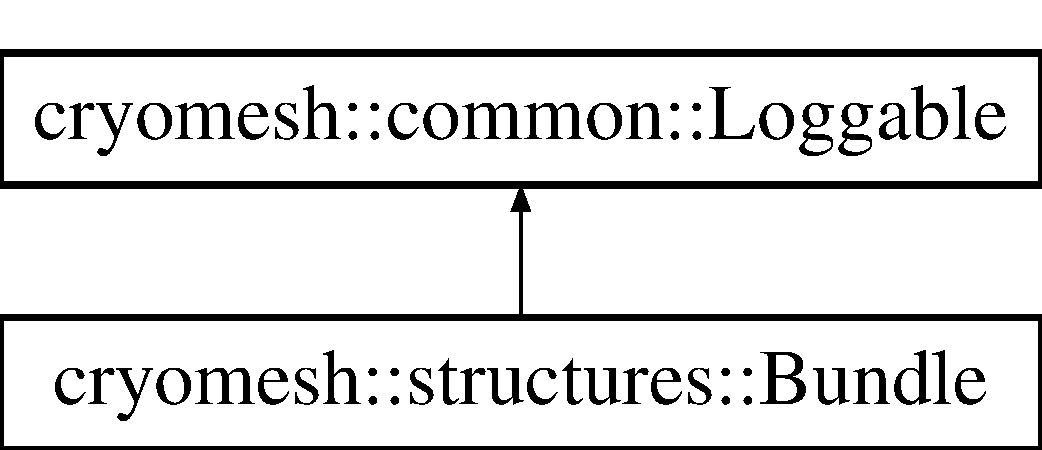
\includegraphics[height=2.000000cm]{classcryomesh_1_1structures_1_1Bundle}
\end{center}
\end{figure}
\subsection*{\-Public \-Types}
\begin{DoxyCompactItemize}
\item 
enum \hyperlink{classcryomesh_1_1common_1_1Loggable_a4d85401f6c81bc8ed94e49d66ae574c5}{\-Logging\-Depth} \{ \hyperlink{classcryomesh_1_1common_1_1Loggable_a4d85401f6c81bc8ed94e49d66ae574c5a51f5abcf5a53a8930a09b065fc64a44f}{\-S\-U\-M\-M\-A\-R\-Y}, 
\hyperlink{classcryomesh_1_1common_1_1Loggable_a4d85401f6c81bc8ed94e49d66ae574c5ae496af0b41e3b64530b61e315822cc51}{\-M\-A\-X}
 \}
\begin{DoxyCompactList}\small\item\em \-Enum representing print detail. \end{DoxyCompactList}\end{DoxyCompactItemize}
\subsection*{\-Public \-Member \-Functions}
\begin{DoxyCompactItemize}
\item 
\hyperlink{classcryomesh_1_1structures_1_1Bundle_a8d6b95207324291f919f1835b81b1640}{\-Bundle} ()
\begin{DoxyCompactList}\small\item\em \-Default contructor. \end{DoxyCompactList}\item 
virtual \hyperlink{classcryomesh_1_1structures_1_1Bundle_ab2ec2696336dddbae17166c056c2f038}{$\sim$\-Bundle} ()
\begin{DoxyCompactList}\small\item\em \-Default destructor. \end{DoxyCompactList}\item 
void \hyperlink{classcryomesh_1_1structures_1_1Bundle_add5af28ceb5c7722d267ba32810c5df7}{update} ()
\begin{DoxyCompactList}\small\item\em \-Update all bundle components. \end{DoxyCompactList}\item 
virtual boost\-::shared\-\_\-ptr\*
$<$ \hyperlink{classcryomesh_1_1structures_1_1Cluster}{\-Cluster} $>$ \hyperlink{classcryomesh_1_1structures_1_1Bundle_a6228d35bd96caa191bd89096dd260ee2}{create\-Cluster} (int node\-Size, int node\-Connectivity)
\begin{DoxyCompactList}\small\item\em \-Create a cluster with a size and connectivity. \end{DoxyCompactList}\item 
virtual boost\-::shared\-\_\-ptr$<$ \hyperlink{classcryomesh_1_1structures_1_1Fibre}{\-Fibre} $>$ \hyperlink{classcryomesh_1_1structures_1_1Bundle_af1884f99e746cdfa549b63f1589b5dac}{connect\-Cluster} (boost\-::uuids\-::uuid input\-Cluster\-U\-U\-I\-D, boost\-::uuids\-::uuid output\-Cluster\-U\-U\-I\-D, int fibre\-Width)
\begin{DoxyCompactList}\small\item\em \-Connect clusters specified by uuids with a fibre of width. \end{DoxyCompactList}\item 
virtual boost\-::shared\-\_\-ptr$<$ \hyperlink{classcryomesh_1_1structures_1_1Fibre}{\-Fibre} $>$ \hyperlink{classcryomesh_1_1structures_1_1Bundle_adc784bc4a171eb28b5a7d038fe73f2de}{connect\-Cluster} (boost\-::uuids\-::uuid cluster\-U\-U\-I\-D, const \hyperlink{classcryomesh_1_1structures_1_1Fibre_aecbba6d46a76f888b3722491b674f5e4}{\-Fibre\-::\-Fibre\-Type} \&type, int fibre\-Width)
\begin{DoxyCompactList}\small\item\em \-Connect clusters specified by uuids with a fibre of width. \end{DoxyCompactList}\item 
virtual boost\-::shared\-\_\-ptr$<$ \hyperlink{classcryomesh_1_1structures_1_1Fibre}{\-Fibre} $>$ \hyperlink{classcryomesh_1_1structures_1_1Bundle_abe23b17f35ef338df7db8d2903ee2bfd}{connect\-Primary\-Input\-Cluster} (boost\-::uuids\-::uuid patchanid, boost\-::uuids\-::uuid cluster\-U\-U\-I\-D)
\begin{DoxyCompactList}\small\item\em \-Helper access function for specialised connection. \end{DoxyCompactList}\item 
virtual boost\-::shared\-\_\-ptr$<$ \hyperlink{classcryomesh_1_1structures_1_1Fibre}{\-Fibre} $>$ \hyperlink{classcryomesh_1_1structures_1_1Bundle_a01dd3e844fe3332df9be5156e329f821}{connect\-Primary\-Output\-Cluster} (boost\-::uuids\-::uuid patchanid, boost\-::uuids\-::uuid cluster\-U\-U\-I\-D)
\begin{DoxyCompactList}\small\item\em \-Helper access function for specialised connection. \end{DoxyCompactList}\item 
std\-::vector$<$ boost\-::shared\-\_\-ptr\*
$<$ \hyperlink{classcryomesh_1_1structures_1_1Fibre}{\-Fibre} $>$ $>$ \hyperlink{classcryomesh_1_1structures_1_1Bundle_a31fef59219384dafb4d250eae65f3574}{auto\-Connect\-Primary\-Input\-Clusters} (const std\-::vector$<$ boost\-::uuids\-::uuid $>$ \&cluster\-\_\-uuids)
\item 
std\-::vector$<$ boost\-::shared\-\_\-ptr\*
$<$ \hyperlink{classcryomesh_1_1structures_1_1Fibre}{\-Fibre} $>$ $>$ \hyperlink{classcryomesh_1_1structures_1_1Bundle_a53f6a455e7cb553352dbef64d3a1ec04}{auto\-Connect\-Primary\-Output\-Clusters} (const std\-::vector$<$ boost\-::uuids\-::uuid $>$ \&cluster\-\_\-uuids)
\item 
virtual std\-::vector\*
$<$ boost\-::shared\-\_\-ptr$<$ \hyperlink{classcryomesh_1_1structures_1_1Fibre}{\-Fibre} $>$ $>$ \hyperlink{classcryomesh_1_1structures_1_1Bundle_aae9fb3393c44f4aeff03ecb8bfa5316e}{auto\-Connect\-Primary\-Input\-Clusters} (std\-::vector$<$ boost\-::shared\-\_\-ptr$<$ \hyperlink{classcryomesh_1_1structures_1_1Cluster}{\-Cluster} $>$ $>$ list)
\item 
virtual std\-::vector\*
$<$ boost\-::shared\-\_\-ptr$<$ \hyperlink{classcryomesh_1_1structures_1_1Fibre}{\-Fibre} $>$ $>$ \hyperlink{classcryomesh_1_1structures_1_1Bundle_a7e38b0167e7873fea9d768d3b096a9d8}{auto\-Connect\-Primary\-Output\-Clusters} (std\-::vector$<$ boost\-::shared\-\_\-ptr$<$ \hyperlink{classcryomesh_1_1structures_1_1Cluster}{\-Cluster} $>$ $>$ list)
\item 
virtual std\-::vector\*
$<$ boost\-::shared\-\_\-ptr\*
$<$ \hyperlink{classcryomesh_1_1state_1_1PatternChannel}{state\-::\-Pattern\-Channel} $>$ $>$ \hyperlink{classcryomesh_1_1structures_1_1Bundle_a6f400ee92f49fed82ca9ef5b48cde285}{get\-Disconnected\-Real\-Input\-Pattern\-Channels} ()
\item 
virtual std\-::vector\*
$<$ boost\-::shared\-\_\-ptr\*
$<$ \hyperlink{classcryomesh_1_1state_1_1PatternChannel}{state\-::\-Pattern\-Channel} $>$ $>$ \hyperlink{classcryomesh_1_1structures_1_1Bundle_a5ce1e31c814ef83026c0dbda5ba04a24}{get\-Disconnected\-Real\-Output\-Pattern\-Channels} ()
\item 
virtual boost\-::shared\-\_\-ptr$<$ \hyperlink{classcryomesh_1_1structures_1_1Fibre}{\-Fibre} $>$ \hyperlink{classcryomesh_1_1structures_1_1Bundle_a0aa4399de46de8ee753e3959fca2fb62}{connect\-Loopback\-Cluster} (boost\-::uuids\-::uuid cluster\-U\-U\-I\-D, int fibre\-Width)
\begin{DoxyCompactList}\small\item\em \-Helper access function for specialised connection. \end{DoxyCompactList}\item 
virtual void \hyperlink{classcryomesh_1_1structures_1_1Bundle_ad60a89acf924c5aebae3a5f816f358db}{load\-Channels} (const std\-::string \&ifstr)
\begin{DoxyCompactList}\small\item\em \-Load in the pattern channels from a filename of a pattern dataset. \end{DoxyCompactList}\item 
const \-Cluster\-Map \& \hyperlink{classcryomesh_1_1structures_1_1Bundle_a181e1f2aaa3b529b8609917d5b5315e0}{get\-Clusters} () const 
\begin{DoxyCompactList}\small\item\em \-Get the clusters in this bundle. \end{DoxyCompactList}\item 
const \hyperlink{classcryomesh_1_1structures_1_1FibreMap}{\-Fibre\-Map} \& \hyperlink{classcryomesh_1_1structures_1_1Bundle_a8f112d3b34f84511781879217b15c6d2}{get\-Fibres} () const 
\begin{DoxyCompactList}\small\item\em \-Get the mutable clusters in this bundle. \end{DoxyCompactList}\item 
const \hyperlink{classcryomesh_1_1structures_1_1FibreMap}{\-Fibre\-Map} \& \hyperlink{classcryomesh_1_1structures_1_1Bundle_a5c6496d00065462122a71c812fa7a4e8}{get\-Input\-Fibres} () const 
\begin{DoxyCompactList}\small\item\em \-Get the input fibres of this bundle. \end{DoxyCompactList}\item 
\hyperlink{classcryomesh_1_1structures_1_1FibreMap}{\-Fibre\-Map} \& \hyperlink{classcryomesh_1_1structures_1_1Bundle_af8b848abb7ec12997b09c63c0c10650d}{get\-Mutable\-Input\-Fibres} ()
\begin{DoxyCompactList}\small\item\em \-Get the mutable input fibres of this bundle. \end{DoxyCompactList}\item 
const \hyperlink{classcryomesh_1_1structures_1_1FibreMap}{\-Fibre\-Map} \& \hyperlink{classcryomesh_1_1structures_1_1Bundle_a2c14a3f2cc96236bff6548e5103183de}{get\-Output\-Fibres} () const 
\begin{DoxyCompactList}\small\item\em \-Get the output fibres of this bundle. \end{DoxyCompactList}\item 
\hyperlink{classcryomesh_1_1structures_1_1FibreMap}{\-Fibre\-Map} \& \hyperlink{classcryomesh_1_1structures_1_1Bundle_af9fd12e753bab64750f5c32d5f17a554}{get\-Mutable\-Output\-Fibres} ()
\begin{DoxyCompactList}\small\item\em \-Get the mutable output fibres of this bundle. \end{DoxyCompactList}\item 
const \hyperlink{classcryomesh_1_1state_1_1PatternChannelMap}{state\-::\-Pattern\-Channel\-Map} \& \hyperlink{classcryomesh_1_1structures_1_1Bundle_ada0ae8374d27d9b59ca82b8075fbd401}{get\-Real\-Input\-Channels\-Map} () const 
\begin{DoxyCompactList}\small\item\em \-Get the real input pattern channels of this bundle. \end{DoxyCompactList}\item 
const \hyperlink{classcryomesh_1_1state_1_1PatternChannelMap}{state\-::\-Pattern\-Channel\-Map} \& \hyperlink{classcryomesh_1_1structures_1_1Bundle_a893be908a14ecc2d07270273d3d127e2}{get\-Real\-Output\-Channels\-Map} () const 
\begin{DoxyCompactList}\small\item\em \-Get the real output pattern channels of this bundle. \end{DoxyCompactList}\item 
const \hyperlink{classcryomesh_1_1state_1_1PatternChannelMap}{state\-::\-Pattern\-Channel\-Map} \& \hyperlink{classcryomesh_1_1structures_1_1Bundle_a65bf0246390e7cb0e90caf4fb302fa41}{get\-Actual\-Input\-Channels\-Map} () const 
\begin{DoxyCompactList}\small\item\em \-Get the actual input pattern channels of this bundle. \end{DoxyCompactList}\item 
const \hyperlink{classcryomesh_1_1state_1_1PatternChannelMap}{state\-::\-Pattern\-Channel\-Map} \& \hyperlink{classcryomesh_1_1structures_1_1Bundle_a382242e3b29b92b25edc9162aa810ebe}{get\-Actual\-Output\-Channels\-Map} () const 
\begin{DoxyCompactList}\small\item\em \-Get the real output pattern channels of this bundle. \end{DoxyCompactList}\item 
const std\-::map\*
$<$ boost\-::uuids\-::uuid, \*
boost\-::uuids\-::uuid $>$ \& \hyperlink{classcryomesh_1_1structures_1_1Bundle_a2e31be3bab4a15e4e9ba6aeac48b91df}{get\-Real\-Fibre\-Pattern\-Channel\-Map} () const 
\begin{DoxyCompactList}\small\item\em \-Get the map of fibres to their associated pattern channels. \end{DoxyCompactList}\item 
const std\-::map\*
$<$ boost\-::uuids\-::uuid, \*
boost\-::uuids\-::uuid $>$ \& \hyperlink{classcryomesh_1_1structures_1_1Bundle_a872de96a76f772182eda2abbb98a99cc}{get\-Actual\-Fibre\-Pattern\-Channel\-Map} () const 
\item 
const boost\-::shared\-\_\-ptr\*
$<$ \hyperlink{classcryomesh_1_1utilities_1_1Statistician}{utilities\-::\-Statistician} $>$ \hyperlink{classcryomesh_1_1structures_1_1Bundle_a5bfac318b9a6f9f651fad0657b9b9196}{get\-Statistician} () const 
\begin{DoxyCompactList}\small\item\em \-Get the \-Statistician. \end{DoxyCompactList}\item 
boost\-::shared\-\_\-ptr\*
$<$ \hyperlink{classcryomesh_1_1utilities_1_1Statistician}{utilities\-::\-Statistician} $>$ \hyperlink{classcryomesh_1_1structures_1_1Bundle_ae750ab1bd2b1a937f90d97e416aefced}{get\-Mutable\-Statistician} ()
\item 
double \hyperlink{classcryomesh_1_1structures_1_1Bundle_aec88635d8c4fdc76b6c3c22b915ee459}{get\-Energy} () const 
\begin{DoxyCompactList}\small\item\em \-Get the last calculated energy of the bundle. \end{DoxyCompactList}\item 
virtual bool \hyperlink{classcryomesh_1_1structures_1_1Bundle_a5927b1a21111e6b78c143280c49a9701}{check\-Structure} () const 
\begin{DoxyCompactList}\small\item\em \-Run a system structure check. \end{DoxyCompactList}\item 
virtual bool \hyperlink{classcryomesh_1_1structures_1_1Bundle_a441eda1670224083d5efc20b3a6bb9ff}{check\-Fibre\-Structure} () const 
\begin{DoxyCompactList}\small\item\em \-Check the structure of \-Fibres. \end{DoxyCompactList}\item 
virtual bool \hyperlink{classcryomesh_1_1structures_1_1Bundle_a1c1b3a4fe6d32259753d69c8a9b0deaa}{check\-Channel\-Structure} () const 
\begin{DoxyCompactList}\small\item\em \-Check the structure of \-Channels. \end{DoxyCompactList}\item 
virtual void \hyperlink{classcryomesh_1_1structures_1_1Bundle_abe63fcceae95f0ffb06db094076b42c5}{enable\-Debug} (bool b)
\item 
virtual void \hyperlink{classcryomesh_1_1structures_1_1Bundle_a8e7f1752b8b0112adf8939921eff4e50}{enable\-Debug\-Clusters} (bool b)
\item 
virtual void \hyperlink{classcryomesh_1_1structures_1_1Bundle_a742597fd733573d8242966f89f8e6715}{enable\-Debug\-Fibres} (bool b)
\item 
virtual std\-::ostream \& \hyperlink{classcryomesh_1_1structures_1_1Bundle_a1b2bdda71a78b4e89af23f21e7611ee4}{print} (std\-::ostream \&os, const \hyperlink{classcryomesh_1_1common_1_1Loggable_a4d85401f6c81bc8ed94e49d66ae574c5}{common\-::\-Loggable\-::\-Logging\-Depth} depth=\hyperlink{classcryomesh_1_1common_1_1Loggable_a4d85401f6c81bc8ed94e49d66ae574c5a51f5abcf5a53a8930a09b065fc64a44f}{\-S\-U\-M\-M\-A\-R\-Y}) const 
\begin{DoxyCompactList}\small\item\em \-Print the bundle to stream. \end{DoxyCompactList}\item 
std\-::ostream \& \hyperlink{classcryomesh_1_1structures_1_1Bundle_ad794a923f68c51c5c1ac4588586b6be7}{print\-Channels} (std\-::ostream \&os) const 
\begin{DoxyCompactList}\small\item\em \-Print the channels to stream. \end{DoxyCompactList}\item 
std\-::ostream \& \hyperlink{classcryomesh_1_1structures_1_1Bundle_ab7308eec882450980ebfbb7167a3538d}{print\-Fibre\-Maps} (std\-::ostream \&os) const 
\item 
std\-::ostream \& \hyperlink{classcryomesh_1_1structures_1_1Bundle_a6a6110f318167f4cc82ab6736e291628}{print\-Fibre\-Map} (std\-::ostream \&os, const std\-::map$<$ boost\-::uuids\-::uuid, boost\-::uuids\-::uuid $>$ \&fibre\-\_\-map) const 
\end{DoxyCompactItemize}
\subsection*{\-Protected \-Member \-Functions}
\begin{DoxyCompactItemize}
\item 
virtual void \hyperlink{classcryomesh_1_1structures_1_1Bundle_abe52d8718eeb7bb6a17211d4dfbed440}{update\-Primary\-Input\-Fibres} ()
\begin{DoxyCompactList}\small\item\em \-Get the next patterns from channels and apply them to their mapped fibres. \end{DoxyCompactList}\item 
virtual void \hyperlink{classcryomesh_1_1structures_1_1Bundle_a7a95265553776d6216799e143134a59f}{update\-Primary\-Output\-Fibres} ()
\begin{DoxyCompactList}\small\item\em \-Get the patterns from primary output fibres and apply them to their mapped pattern channels. \end{DoxyCompactList}\item 
virtual double \hyperlink{classcryomesh_1_1structures_1_1Bundle_a3a8a7cfb5d525ff59a52dd1a39909621}{match\-Output\-Channels\-Sum} () const 
\begin{DoxyCompactList}\small\item\em \-Compare the output channels of primary output fibres to expected output channel patterns. \end{DoxyCompactList}\item 
virtual void \hyperlink{classcryomesh_1_1structures_1_1Bundle_a804c625c912657cebd3350c7c1b53c10}{update\-Statistician} ()
\begin{DoxyCompactList}\small\item\em \-Update the statistician if debugging is enabled. \end{DoxyCompactList}\item 
void \hyperlink{classcryomesh_1_1structures_1_1Bundle_ae6a553eaab4ddf2b6bbd6bdeca9361ad}{set\-Energy} (double d)
\begin{DoxyCompactList}\small\item\em \-Set the energy of the bundle. \end{DoxyCompactList}\item 
\-Cluster\-Map \& \hyperlink{classcryomesh_1_1structures_1_1Bundle_a14990ba8cec7b9c18426ae8c2fdd0dcf}{get\-Mutable\-Clusters} ()
\item 
{\footnotesize template$<$class T $>$ }\\std\-::ostream \& \hyperlink{classcryomesh_1_1structures_1_1Bundle_af89da428bb056c8eea81a416783cf2ae}{print\-Search} (std\-::ostream \&os, const boost\-::uuids\-::uuid \&uuid, const std\-::map$<$ boost\-::uuids\-::uuid, boost\-::shared\-\_\-ptr$<$ \-T $>$ $>$ \&map) const 
\begin{DoxyCompactList}\small\item\em \-Print out a uuid search. \end{DoxyCompactList}\end{DoxyCompactItemize}
\subsection*{\-Private \-Member \-Functions}
\begin{DoxyCompactItemize}
\item 
const boost\-::shared\-\_\-ptr\*
$<$ \hyperlink{classcryomesh_1_1state_1_1PatternChannel}{state\-::\-Pattern\-Channel} $>$ \hyperlink{classcryomesh_1_1structures_1_1Bundle_a51eb35ecb02094016f0f3a74fd07f6e9}{get\-Real\-Primary\-Input\-Channel\-By\-Fibre} (const boost\-::uuids\-::uuid fibre\-\_\-uuid) const 
\item 
const boost\-::shared\-\_\-ptr\*
$<$ \hyperlink{classcryomesh_1_1state_1_1PatternChannel}{state\-::\-Pattern\-Channel} $>$ \hyperlink{classcryomesh_1_1structures_1_1Bundle_a00eb0f18cc3331a4e6d0ed4698e92cb5}{get\-Real\-Primary\-Output\-Channel\-By\-Fibre} (const boost\-::uuids\-::uuid fibre\-\_\-uuid) const 
\item 
const boost\-::shared\-\_\-ptr\*
$<$ \hyperlink{classcryomesh_1_1state_1_1PatternChannel}{state\-::\-Pattern\-Channel} $>$ \hyperlink{classcryomesh_1_1structures_1_1Bundle_a101bda3e32c34cf8e0cff4526446af02}{get\-Actual\-Primary\-Input\-Channel\-By\-Fibre} (const boost\-::uuids\-::uuid fibre\-\_\-uuid) const 
\item 
const boost\-::shared\-\_\-ptr\*
$<$ \hyperlink{classcryomesh_1_1state_1_1PatternChannel}{state\-::\-Pattern\-Channel} $>$ \hyperlink{classcryomesh_1_1structures_1_1Bundle_a13dcea26d3379199f9e993caa5e132d7}{get\-Actual\-Primary\-Output\-Channel\-By\-Fibre} (const boost\-::uuids\-::uuid fibre\-\_\-uuid) const 
\item 
const boost\-::shared\-\_\-ptr$<$ \hyperlink{classcryomesh_1_1structures_1_1Fibre}{\-Fibre} $>$ \hyperlink{classcryomesh_1_1structures_1_1Bundle_ae1259ecf25a6b140cad735defd9069f9}{get\-Primary\-Input\-Fibre\-By\-Real\-Channel} (const boost\-::uuids\-::uuid pattern\-\_\-channel\-\_\-uuid) const 
\begin{DoxyCompactList}\small\item\em \-Helper method to take a uuid and find its correspondingly mapped object \-Take an input \-Pattern\-Channel uuid and find the input \hyperlink{classcryomesh_1_1structures_1_1Fibre}{\-Fibre} its mapped to. \end{DoxyCompactList}\item 
const boost\-::shared\-\_\-ptr$<$ \hyperlink{classcryomesh_1_1structures_1_1Fibre}{\-Fibre} $>$ \hyperlink{classcryomesh_1_1structures_1_1Bundle_a7ba3f747f8e164f0c0984fdb14922e7a}{get\-Primary\-Output\-Fibre\-By\-Real\-Channel} (const boost\-::uuids\-::uuid pattern\-\_\-channel\-\_\-uuid) const 
\begin{DoxyCompactList}\small\item\em \-Helper method to take a uuid and find its correspondingly mapped object \-Take an output \-Pattern\-Channel uuid and find the output \hyperlink{classcryomesh_1_1structures_1_1Fibre}{\-Fibre} its mapped to. \end{DoxyCompactList}\item 
const boost\-::shared\-\_\-ptr$<$ \hyperlink{classcryomesh_1_1structures_1_1Fibre}{\-Fibre} $>$ \hyperlink{classcryomesh_1_1structures_1_1Bundle_ad80f4bbb8bdc379e156282bf0b17fbc3}{get\-Primary\-Input\-Fibre\-By\-Actual\-Channel} (const boost\-::uuids\-::uuid pattern\-\_\-channel\-\_\-uuid) const 
\item 
const boost\-::shared\-\_\-ptr$<$ \hyperlink{classcryomesh_1_1structures_1_1Fibre}{\-Fibre} $>$ \hyperlink{classcryomesh_1_1structures_1_1Bundle_ae6ccd53821a90466d96ebcbf171549a2}{get\-Primary\-Output\-Fibre\-By\-Actual\-Channel} (const boost\-::uuids\-::uuid pattern\-\_\-channel\-\_\-uuid) const 
\item 
const boost\-::shared\-\_\-ptr$<$ \hyperlink{classcryomesh_1_1structures_1_1Fibre}{\-Fibre} $>$ \hyperlink{classcryomesh_1_1structures_1_1Bundle_aecdb1fc4017f4e4aa954b4158e99c86f}{get\-Primary\-Fibre\-By\-Channel} (const boost\-::uuids\-::uuid id, const \hyperlink{classcryomesh_1_1structures_1_1FibreMap}{\-Fibre\-Map} \&map, const std\-::map$<$ boost\-::uuids\-::uuid, boost\-::uuids\-::uuid $>$ \&fibrepattern\-\_\-channelmap) const 
\begin{DoxyCompactList}\small\item\em \-Helper method to take a uuid and find its correspondingly mapped object \-Take an channel uuid and find the \hyperlink{classcryomesh_1_1structures_1_1Fibre}{\-Fibre} its mapped to inside the supplied map. \end{DoxyCompactList}\item 
const boost\-::shared\-\_\-ptr\*
$<$ \hyperlink{classcryomesh_1_1state_1_1PatternChannel}{state\-::\-Pattern\-Channel} $>$ \hyperlink{classcryomesh_1_1structures_1_1Bundle_a237b9698b966c6498fb723f685292599}{get\-Primary\-Channel\-By\-Fibre} (const boost\-::uuids\-::uuid id, const \hyperlink{classcryomesh_1_1state_1_1PatternChannelMap}{state\-::\-Pattern\-Channel\-Map} \&map, const std\-::map$<$ boost\-::uuids\-::uuid, boost\-::uuids\-::uuid $>$ \&fibrepattern\-\_\-channelmap) const 
\begin{DoxyCompactList}\small\item\em \-Helper method to take a uuid and find its correspondingly mapped object \-Take an \hyperlink{classcryomesh_1_1structures_1_1Fibre}{\-Fibre} uuid and find the \-Pattern\-Channel its mapped to inside the supplied map. \end{DoxyCompactList}\end{DoxyCompactItemize}
\subsection*{\-Private \-Attributes}
\begin{DoxyCompactItemize}
\item 
\-Cluster\-Map \hyperlink{classcryomesh_1_1structures_1_1Bundle_a35a36d3305706f597f4c586fcd9f74b7}{clusters}
\item 
\hyperlink{classcryomesh_1_1structures_1_1FibreMap}{\-Fibre\-Map} \hyperlink{classcryomesh_1_1structures_1_1Bundle_a71b3308a867169b8e9af9ab71b8bdf98}{fibres}
\item 
\hyperlink{classcryomesh_1_1state_1_1PatternChannelMap}{state\-::\-Pattern\-Channel\-Map} \hyperlink{classcryomesh_1_1structures_1_1Bundle_ac9bd1c696001ef8acb7291a5f9e81c8b}{real\-Input\-Channels\-Map}
\item 
\hyperlink{classcryomesh_1_1state_1_1PatternChannelMap}{state\-::\-Pattern\-Channel\-Map} \hyperlink{classcryomesh_1_1structures_1_1Bundle_a4043d8bfeb8b066418029864f51d92de}{real\-Output\-Channels\-Map}
\item 
\hyperlink{classcryomesh_1_1state_1_1PatternChannelMap}{state\-::\-Pattern\-Channel\-Map} \hyperlink{classcryomesh_1_1structures_1_1Bundle_ae20b2f9819708971357148dd024db00d}{actual\-Input\-Channels\-Map}
\item 
\hyperlink{classcryomesh_1_1state_1_1PatternChannelMap}{state\-::\-Pattern\-Channel\-Map} \hyperlink{classcryomesh_1_1structures_1_1Bundle_ac67a6d7b29b37b8927c93350e8bcf6e5}{actual\-Output\-Channels\-Map}
\item 
\hyperlink{classcryomesh_1_1structures_1_1FibreMap}{\-Fibre\-Map} \hyperlink{classcryomesh_1_1structures_1_1Bundle_aa6a461295021bdfb4ef4cab0f136a2c1}{input\-Fibres}
\item 
\hyperlink{classcryomesh_1_1structures_1_1FibreMap}{\-Fibre\-Map} \hyperlink{classcryomesh_1_1structures_1_1Bundle_aa671193358b7aba173e45574def3d4c1}{output\-Fibres}
\item 
boost\-::shared\-\_\-ptr\*
$<$ \hyperlink{classcryomesh_1_1utilities_1_1Statistician}{utilities\-::\-Statistician} $>$ \hyperlink{classcryomesh_1_1structures_1_1Bundle_ad505cbda03b4e78399fd3a9568d79708}{statistician}
\begin{DoxyCompactList}\small\item\em \-Statistics object to generate useful info on the bundle. \end{DoxyCompactList}\item 
double \hyperlink{classcryomesh_1_1structures_1_1Bundle_aac5229c4c52e646767db2144ba745aa6}{energy}
\begin{DoxyCompactList}\small\item\em \-Last energy calculation of the output channel matching. \end{DoxyCompactList}\item 
std\-::map$<$ boost\-::uuids\-::uuid, \*
boost\-::uuids\-::uuid $>$ \hyperlink{classcryomesh_1_1structures_1_1Bundle_adaf7fa91209de01b9d42ae2d8228c3cd}{real\-Fibre\-Pattern\-Channel\-Map}
\item 
std\-::map$<$ boost\-::uuids\-::uuid, \*
boost\-::uuids\-::uuid $>$ \hyperlink{classcryomesh_1_1structures_1_1Bundle_a0f3e20833ce850f97ae450d27a4607dd}{actual\-Fibre\-Pattern\-Channel\-Map}
\item 
\hyperlink{classcryomesh_1_1structures_1_1Cluster_a69c420b79675c6ffc9a0df8381ca9497}{\-Cluster\-::\-Energy\-Fraction\-Method} \hyperlink{classcryomesh_1_1structures_1_1Bundle_abbd8555380ffa4c33a235636837bafaa}{energy\-Fraction\-Method}
\end{DoxyCompactItemize}
\subsection*{\-Friends}
\begin{DoxyCompactItemize}
\item 
std\-::ostream \& \hyperlink{classcryomesh_1_1structures_1_1Bundle_a21e43a0b5ea3e93accc964e269c730bd}{operator$<$$<$} (std\-::ostream \&os, const \hyperlink{classcryomesh_1_1structures_1_1Bundle}{\-Bundle} \&obj)
\begin{DoxyCompactList}\small\item\em \-To stream operator. \end{DoxyCompactList}\end{DoxyCompactItemize}


\subsection{\-Detailed \-Description}
\-A \hyperlink{classcryomesh_1_1structures_1_1Bundle}{\-Bundle} is the collection of clusters and fibres, it represents the system as a whole. 

\-Definition at line 29 of file \-Bundle.\-h.



\subsection{\-Member \-Enumeration \-Documentation}
\hypertarget{classcryomesh_1_1common_1_1Loggable_a4d85401f6c81bc8ed94e49d66ae574c5}{\index{cryomesh\-::structures\-::\-Bundle@{cryomesh\-::structures\-::\-Bundle}!\-Logging\-Depth@{\-Logging\-Depth}}
\index{\-Logging\-Depth@{\-Logging\-Depth}!cryomesh::structures::Bundle@{cryomesh\-::structures\-::\-Bundle}}
\subsubsection[{\-Logging\-Depth}]{\setlength{\rightskip}{0pt plus 5cm}enum {\bf cryomesh\-::common\-::\-Loggable\-::\-Logging\-Depth}\hspace{0.3cm}{\ttfamily  \mbox{[}inherited\mbox{]}}}}\label{classcryomesh_1_1common_1_1Loggable_a4d85401f6c81bc8ed94e49d66ae574c5}


\-Enum representing print detail. 

\begin{Desc}
\item[\-Enumerator\-: ]\par
\begin{description}
\index{\-S\-U\-M\-M\-A\-R\-Y@{\-S\-U\-M\-M\-A\-R\-Y}!cryomesh\-::structures\-::\-Bundle@{cryomesh\-::structures\-::\-Bundle}}\index{cryomesh\-::structures\-::\-Bundle@{cryomesh\-::structures\-::\-Bundle}!\-S\-U\-M\-M\-A\-R\-Y@{\-S\-U\-M\-M\-A\-R\-Y}}\item[{\em 
\hypertarget{classcryomesh_1_1common_1_1Loggable_a4d85401f6c81bc8ed94e49d66ae574c5a51f5abcf5a53a8930a09b065fc64a44f}{\-S\-U\-M\-M\-A\-R\-Y}\label{classcryomesh_1_1common_1_1Loggable_a4d85401f6c81bc8ed94e49d66ae574c5a51f5abcf5a53a8930a09b065fc64a44f}
}]\index{\-M\-A\-X@{\-M\-A\-X}!cryomesh\-::structures\-::\-Bundle@{cryomesh\-::structures\-::\-Bundle}}\index{cryomesh\-::structures\-::\-Bundle@{cryomesh\-::structures\-::\-Bundle}!\-M\-A\-X@{\-M\-A\-X}}\item[{\em 
\hypertarget{classcryomesh_1_1common_1_1Loggable_a4d85401f6c81bc8ed94e49d66ae574c5ae496af0b41e3b64530b61e315822cc51}{\-M\-A\-X}\label{classcryomesh_1_1common_1_1Loggable_a4d85401f6c81bc8ed94e49d66ae574c5ae496af0b41e3b64530b61e315822cc51}
}]\end{description}
\end{Desc}



\-Definition at line 23 of file \-Loggable.\-h.



\subsection{\-Constructor \& \-Destructor \-Documentation}
\hypertarget{classcryomesh_1_1structures_1_1Bundle_a8d6b95207324291f919f1835b81b1640}{\index{cryomesh\-::structures\-::\-Bundle@{cryomesh\-::structures\-::\-Bundle}!\-Bundle@{\-Bundle}}
\index{\-Bundle@{\-Bundle}!cryomesh::structures::Bundle@{cryomesh\-::structures\-::\-Bundle}}
\subsubsection[{\-Bundle}]{\setlength{\rightskip}{0pt plus 5cm}{\bf cryomesh\-::structures\-::\-Bundle\-::\-Bundle} (
\begin{DoxyParamCaption}
{}
\end{DoxyParamCaption}
)}}\label{classcryomesh_1_1structures_1_1Bundle_a8d6b95207324291f919f1835b81b1640}


\-Default contructor. 



\-Definition at line 17 of file \-Bundle.\-cpp.

\hypertarget{classcryomesh_1_1structures_1_1Bundle_ab2ec2696336dddbae17166c056c2f038}{\index{cryomesh\-::structures\-::\-Bundle@{cryomesh\-::structures\-::\-Bundle}!$\sim$\-Bundle@{$\sim$\-Bundle}}
\index{$\sim$\-Bundle@{$\sim$\-Bundle}!cryomesh::structures::Bundle@{cryomesh\-::structures\-::\-Bundle}}
\subsubsection[{$\sim$\-Bundle}]{\setlength{\rightskip}{0pt plus 5cm}{\bf cryomesh\-::structures\-::\-Bundle\-::$\sim$\-Bundle} (
\begin{DoxyParamCaption}
{}
\end{DoxyParamCaption}
)\hspace{0.3cm}{\ttfamily  \mbox{[}virtual\mbox{]}}}}\label{classcryomesh_1_1structures_1_1Bundle_ab2ec2696336dddbae17166c056c2f038}


\-Default destructor. 



\-Definition at line 23 of file \-Bundle.\-cpp.



\subsection{\-Member \-Function \-Documentation}
\hypertarget{classcryomesh_1_1structures_1_1Bundle_a31fef59219384dafb4d250eae65f3574}{\index{cryomesh\-::structures\-::\-Bundle@{cryomesh\-::structures\-::\-Bundle}!auto\-Connect\-Primary\-Input\-Clusters@{auto\-Connect\-Primary\-Input\-Clusters}}
\index{auto\-Connect\-Primary\-Input\-Clusters@{auto\-Connect\-Primary\-Input\-Clusters}!cryomesh::structures::Bundle@{cryomesh\-::structures\-::\-Bundle}}
\subsubsection[{auto\-Connect\-Primary\-Input\-Clusters}]{\setlength{\rightskip}{0pt plus 5cm}std\-::vector$<$ boost\-::shared\-\_\-ptr$<$ {\bf \-Fibre} $>$ $>$ {\bf cryomesh\-::structures\-::\-Bundle\-::auto\-Connect\-Primary\-Input\-Clusters} (
\begin{DoxyParamCaption}
\item[{const std\-::vector$<$ boost\-::uuids\-::uuid $>$ \&}]{cluster\-\_\-uuids}
\end{DoxyParamCaption}
)}}\label{classcryomesh_1_1structures_1_1Bundle_a31fef59219384dafb4d250eae65f3574}


\-Definition at line 206 of file \-Bundle.\-cpp.



\-References get\-Mutable\-Clusters().

\hypertarget{classcryomesh_1_1structures_1_1Bundle_aae9fb3393c44f4aeff03ecb8bfa5316e}{\index{cryomesh\-::structures\-::\-Bundle@{cryomesh\-::structures\-::\-Bundle}!auto\-Connect\-Primary\-Input\-Clusters@{auto\-Connect\-Primary\-Input\-Clusters}}
\index{auto\-Connect\-Primary\-Input\-Clusters@{auto\-Connect\-Primary\-Input\-Clusters}!cryomesh::structures::Bundle@{cryomesh\-::structures\-::\-Bundle}}
\subsubsection[{auto\-Connect\-Primary\-Input\-Clusters}]{\setlength{\rightskip}{0pt plus 5cm}std\-::vector$<$ boost\-::shared\-\_\-ptr$<$ {\bf \-Fibre} $>$ $>$ {\bf cryomesh\-::structures\-::\-Bundle\-::auto\-Connect\-Primary\-Input\-Clusters} (
\begin{DoxyParamCaption}
\item[{std\-::vector$<$ boost\-::shared\-\_\-ptr$<$ {\bf \-Cluster} $>$ $>$}]{list}
\end{DoxyParamCaption}
)\hspace{0.3cm}{\ttfamily  \mbox{[}virtual\mbox{]}}}}\label{classcryomesh_1_1structures_1_1Bundle_aae9fb3393c44f4aeff03ecb8bfa5316e}


\-Definition at line 254 of file \-Bundle.\-cpp.



\-References connect\-Primary\-Input\-Cluster(), and get\-Disconnected\-Real\-Input\-Pattern\-Channels().

\hypertarget{classcryomesh_1_1structures_1_1Bundle_a53f6a455e7cb553352dbef64d3a1ec04}{\index{cryomesh\-::structures\-::\-Bundle@{cryomesh\-::structures\-::\-Bundle}!auto\-Connect\-Primary\-Output\-Clusters@{auto\-Connect\-Primary\-Output\-Clusters}}
\index{auto\-Connect\-Primary\-Output\-Clusters@{auto\-Connect\-Primary\-Output\-Clusters}!cryomesh::structures::Bundle@{cryomesh\-::structures\-::\-Bundle}}
\subsubsection[{auto\-Connect\-Primary\-Output\-Clusters}]{\setlength{\rightskip}{0pt plus 5cm}std\-::vector$<$ boost\-::shared\-\_\-ptr$<$ {\bf \-Fibre} $>$ $>$ {\bf cryomesh\-::structures\-::\-Bundle\-::auto\-Connect\-Primary\-Output\-Clusters} (
\begin{DoxyParamCaption}
\item[{const std\-::vector$<$ boost\-::uuids\-::uuid $>$ \&}]{cluster\-\_\-uuids}
\end{DoxyParamCaption}
)}}\label{classcryomesh_1_1structures_1_1Bundle_a53f6a455e7cb553352dbef64d3a1ec04}


\-Definition at line 231 of file \-Bundle.\-cpp.



\-References get\-Mutable\-Clusters().

\hypertarget{classcryomesh_1_1structures_1_1Bundle_a7e38b0167e7873fea9d768d3b096a9d8}{\index{cryomesh\-::structures\-::\-Bundle@{cryomesh\-::structures\-::\-Bundle}!auto\-Connect\-Primary\-Output\-Clusters@{auto\-Connect\-Primary\-Output\-Clusters}}
\index{auto\-Connect\-Primary\-Output\-Clusters@{auto\-Connect\-Primary\-Output\-Clusters}!cryomesh::structures::Bundle@{cryomesh\-::structures\-::\-Bundle}}
\subsubsection[{auto\-Connect\-Primary\-Output\-Clusters}]{\setlength{\rightskip}{0pt plus 5cm}std\-::vector$<$ boost\-::shared\-\_\-ptr$<$ {\bf \-Fibre} $>$ $>$ {\bf cryomesh\-::structures\-::\-Bundle\-::auto\-Connect\-Primary\-Output\-Clusters} (
\begin{DoxyParamCaption}
\item[{std\-::vector$<$ boost\-::shared\-\_\-ptr$<$ {\bf \-Cluster} $>$ $>$}]{list}
\end{DoxyParamCaption}
)\hspace{0.3cm}{\ttfamily  \mbox{[}virtual\mbox{]}}}}\label{classcryomesh_1_1structures_1_1Bundle_a7e38b0167e7873fea9d768d3b096a9d8}


\-Definition at line 301 of file \-Bundle.\-cpp.



\-References connect\-Primary\-Output\-Cluster(), and get\-Disconnected\-Real\-Output\-Pattern\-Channels().

\hypertarget{classcryomesh_1_1structures_1_1Bundle_a1c1b3a4fe6d32259753d69c8a9b0deaa}{\index{cryomesh\-::structures\-::\-Bundle@{cryomesh\-::structures\-::\-Bundle}!check\-Channel\-Structure@{check\-Channel\-Structure}}
\index{check\-Channel\-Structure@{check\-Channel\-Structure}!cryomesh::structures::Bundle@{cryomesh\-::structures\-::\-Bundle}}
\subsubsection[{check\-Channel\-Structure}]{\setlength{\rightskip}{0pt plus 5cm}bool {\bf cryomesh\-::structures\-::\-Bundle\-::check\-Channel\-Structure} (
\begin{DoxyParamCaption}
{}
\end{DoxyParamCaption}
) const\hspace{0.3cm}{\ttfamily  \mbox{[}virtual\mbox{]}}}}\label{classcryomesh_1_1structures_1_1Bundle_a1c1b3a4fe6d32259753d69c8a9b0deaa}


\-Check the structure of \-Channels. 

\begin{DoxyReturn}{\-Returns}
bool \-True if structure tests pass, false otherwise 
\end{DoxyReturn}


\-Definition at line 558 of file \-Bundle.\-cpp.



\-Referenced by check\-Structure().

\hypertarget{classcryomesh_1_1structures_1_1Bundle_a441eda1670224083d5efc20b3a6bb9ff}{\index{cryomesh\-::structures\-::\-Bundle@{cryomesh\-::structures\-::\-Bundle}!check\-Fibre\-Structure@{check\-Fibre\-Structure}}
\index{check\-Fibre\-Structure@{check\-Fibre\-Structure}!cryomesh::structures::Bundle@{cryomesh\-::structures\-::\-Bundle}}
\subsubsection[{check\-Fibre\-Structure}]{\setlength{\rightskip}{0pt plus 5cm}bool {\bf cryomesh\-::structures\-::\-Bundle\-::check\-Fibre\-Structure} (
\begin{DoxyParamCaption}
{}
\end{DoxyParamCaption}
) const\hspace{0.3cm}{\ttfamily  \mbox{[}virtual\mbox{]}}}}\label{classcryomesh_1_1structures_1_1Bundle_a441eda1670224083d5efc20b3a6bb9ff}


\-Check the structure of \-Fibres. 

\begin{DoxyReturn}{\-Returns}
bool \-True if structure tests pass, false otherwise 
\end{DoxyReturn}


\-Definition at line 477 of file \-Bundle.\-cpp.



\-References get\-Clusters(), get\-Fibres(), get\-Input\-Fibres(), and get\-Output\-Fibres().



\-Referenced by check\-Structure().

\hypertarget{classcryomesh_1_1structures_1_1Bundle_a5927b1a21111e6b78c143280c49a9701}{\index{cryomesh\-::structures\-::\-Bundle@{cryomesh\-::structures\-::\-Bundle}!check\-Structure@{check\-Structure}}
\index{check\-Structure@{check\-Structure}!cryomesh::structures::Bundle@{cryomesh\-::structures\-::\-Bundle}}
\subsubsection[{check\-Structure}]{\setlength{\rightskip}{0pt plus 5cm}bool {\bf cryomesh\-::structures\-::\-Bundle\-::check\-Structure} (
\begin{DoxyParamCaption}
{}
\end{DoxyParamCaption}
) const\hspace{0.3cm}{\ttfamily  \mbox{[}virtual\mbox{]}}}}\label{classcryomesh_1_1structures_1_1Bundle_a5927b1a21111e6b78c143280c49a9701}


\-Run a system structure check. 

\begin{DoxyReturn}{\-Returns}
bool \-True if system passes all tests, false otherwise 
\end{DoxyReturn}


\-Definition at line 561 of file \-Bundle.\-cpp.



\-References check\-Channel\-Structure(), and check\-Fibre\-Structure().

\hypertarget{classcryomesh_1_1structures_1_1Bundle_af1884f99e746cdfa549b63f1589b5dac}{\index{cryomesh\-::structures\-::\-Bundle@{cryomesh\-::structures\-::\-Bundle}!connect\-Cluster@{connect\-Cluster}}
\index{connect\-Cluster@{connect\-Cluster}!cryomesh::structures::Bundle@{cryomesh\-::structures\-::\-Bundle}}
\subsubsection[{connect\-Cluster}]{\setlength{\rightskip}{0pt plus 5cm}boost\-::shared\-\_\-ptr$<$ {\bf \-Fibre} $>$ {\bf cryomesh\-::structures\-::\-Bundle\-::connect\-Cluster} (
\begin{DoxyParamCaption}
\item[{boost\-::uuids\-::uuid}]{input\-Cluster\-U\-U\-I\-D, }
\item[{boost\-::uuids\-::uuid}]{output\-Cluster\-U\-U\-I\-D, }
\item[{int}]{fibre\-Width}
\end{DoxyParamCaption}
)\hspace{0.3cm}{\ttfamily  \mbox{[}virtual\mbox{]}}}}\label{classcryomesh_1_1structures_1_1Bundle_af1884f99e746cdfa549b63f1589b5dac}


\-Connect clusters specified by uuids with a fibre of width. 


\begin{DoxyParams}{\-Parameters}
{\em boost\-::uuids\-::uuid} & input\-Cluster\-U\-U\-I\-D \-U\-U\-I\-D of input cluster \\
\hline
{\em boost\-::uuids\-::uuid} & output\-Cluster\-U\-U\-I\-D \-U\-U\-I\-D of output cluster \\
\hline
{\em int} & width \-Width of fibre to create\\
\hline
\end{DoxyParams}
\begin{DoxyReturn}{\-Returns}
\-The new fibre created, possible null 
\end{DoxyReturn}


\-Definition at line 61 of file \-Bundle.\-cpp.



\-References clusters, and fibres.



\-Referenced by connect\-Loopback\-Cluster(), connect\-Primary\-Input\-Cluster(), and connect\-Primary\-Output\-Cluster().

\hypertarget{classcryomesh_1_1structures_1_1Bundle_adc784bc4a171eb28b5a7d038fe73f2de}{\index{cryomesh\-::structures\-::\-Bundle@{cryomesh\-::structures\-::\-Bundle}!connect\-Cluster@{connect\-Cluster}}
\index{connect\-Cluster@{connect\-Cluster}!cryomesh::structures::Bundle@{cryomesh\-::structures\-::\-Bundle}}
\subsubsection[{connect\-Cluster}]{\setlength{\rightskip}{0pt plus 5cm}boost\-::shared\-\_\-ptr$<$ {\bf \-Fibre} $>$ {\bf cryomesh\-::structures\-::\-Bundle\-::connect\-Cluster} (
\begin{DoxyParamCaption}
\item[{boost\-::uuids\-::uuid}]{cluster\-U\-U\-I\-D, }
\item[{const {\bf \-Fibre\-::\-Fibre\-Type} \&}]{type, }
\item[{int}]{fibre\-Width}
\end{DoxyParamCaption}
)\hspace{0.3cm}{\ttfamily  \mbox{[}virtual\mbox{]}}}}\label{classcryomesh_1_1structures_1_1Bundle_adc784bc4a171eb28b5a7d038fe73f2de}


\-Connect clusters specified by uuids with a fibre of width. 


\begin{DoxyParams}{\-Parameters}
{\em boost\-::uuids\-::uuid} & cluster\-U\-U\-I\-D \-U\-U\-I\-D of cluster to connect to fibre \\
\hline
{\em const} & \hyperlink{classcryomesh_1_1structures_1_1Fibre_aecbba6d46a76f888b3722491b674f5e4}{\-Fibre\-::\-Fibre\-Type} \& type \-Type of fibre connection to make \\
\hline
{\em int} & width \-Width of fibre to create\\
\hline
\end{DoxyParams}
\begin{DoxyReturn}{\-Returns}
\-The new fibre created, possible null 
\end{DoxyReturn}


\-Definition at line 78 of file \-Bundle.\-cpp.



\-References clusters, fibres, input\-Fibres, cryomesh\-::structures\-::\-Fibre\-::\-Loopback\-Fibre, output\-Fibres, cryomesh\-::structures\-::\-Fibre\-::\-Primary\-Input\-Fibre, and cryomesh\-::structures\-::\-Fibre\-::\-Primary\-Output\-Fibre.

\hypertarget{classcryomesh_1_1structures_1_1Bundle_a0aa4399de46de8ee753e3959fca2fb62}{\index{cryomesh\-::structures\-::\-Bundle@{cryomesh\-::structures\-::\-Bundle}!connect\-Loopback\-Cluster@{connect\-Loopback\-Cluster}}
\index{connect\-Loopback\-Cluster@{connect\-Loopback\-Cluster}!cryomesh::structures::Bundle@{cryomesh\-::structures\-::\-Bundle}}
\subsubsection[{connect\-Loopback\-Cluster}]{\setlength{\rightskip}{0pt plus 5cm}boost\-::shared\-\_\-ptr$<$ {\bf \-Fibre} $>$ {\bf cryomesh\-::structures\-::\-Bundle\-::connect\-Loopback\-Cluster} (
\begin{DoxyParamCaption}
\item[{boost\-::uuids\-::uuid}]{cluster\-U\-U\-I\-D, }
\item[{int}]{fibre\-Width}
\end{DoxyParamCaption}
)\hspace{0.3cm}{\ttfamily  \mbox{[}virtual\mbox{]}}}}\label{classcryomesh_1_1structures_1_1Bundle_a0aa4399de46de8ee753e3959fca2fb62}


\-Helper access function for specialised connection. 


\begin{DoxyParams}{\-Parameters}
{\em const} & \hyperlink{classcryomesh_1_1structures_1_1Fibre_aecbba6d46a76f888b3722491b674f5e4}{\-Fibre\-::\-Fibre\-Type} \& type \-Type of fibre connection to make \\
\hline
{\em int} & width \-Width of fibre to create\\
\hline
\end{DoxyParams}
\begin{DoxyReturn}{\-Returns}
\-The new fibre created, possible null 
\end{DoxyReturn}


\-Definition at line 392 of file \-Bundle.\-cpp.



\-References connect\-Cluster(), and cryomesh\-::structures\-::\-Fibre\-::\-Loopback\-Fibre.

\hypertarget{classcryomesh_1_1structures_1_1Bundle_abe23b17f35ef338df7db8d2903ee2bfd}{\index{cryomesh\-::structures\-::\-Bundle@{cryomesh\-::structures\-::\-Bundle}!connect\-Primary\-Input\-Cluster@{connect\-Primary\-Input\-Cluster}}
\index{connect\-Primary\-Input\-Cluster@{connect\-Primary\-Input\-Cluster}!cryomesh::structures::Bundle@{cryomesh\-::structures\-::\-Bundle}}
\subsubsection[{connect\-Primary\-Input\-Cluster}]{\setlength{\rightskip}{0pt plus 5cm}boost\-::shared\-\_\-ptr$<$ {\bf \-Fibre} $>$ {\bf cryomesh\-::structures\-::\-Bundle\-::connect\-Primary\-Input\-Cluster} (
\begin{DoxyParamCaption}
\item[{boost\-::uuids\-::uuid}]{patchanid, }
\item[{boost\-::uuids\-::uuid}]{cluster\-U\-U\-I\-D}
\end{DoxyParamCaption}
)\hspace{0.3cm}{\ttfamily  \mbox{[}virtual\mbox{]}}}}\label{classcryomesh_1_1structures_1_1Bundle_abe23b17f35ef338df7db8d2903ee2bfd}


\-Helper access function for specialised connection. 


\begin{DoxyParams}{\-Parameters}
{\em boost\-::uuids\-::uuid} & \-Pattern\-Channel to map the fibre to \\
\hline
{\em const} & \hyperlink{classcryomesh_1_1structures_1_1Fibre_aecbba6d46a76f888b3722491b674f5e4}{\-Fibre\-::\-Fibre\-Type} \& type \-Type of fibre connection to make\\
\hline
\end{DoxyParams}
\begin{DoxyReturn}{\-Returns}
\-The new fibre created, possible null 
\end{DoxyReturn}


\-Definition at line 110 of file \-Bundle.\-cpp.



\-References actual\-Fibre\-Pattern\-Channel\-Map, actual\-Input\-Channels\-Map, connect\-Cluster(), cryomesh\-::state\-::\-Pattern\-Channel\-::\-Input, cryomesh\-::structures\-::\-Fibre\-::\-Primary\-Input\-Fibre, real\-Fibre\-Pattern\-Channel\-Map, and real\-Input\-Channels\-Map.



\-Referenced by auto\-Connect\-Primary\-Input\-Clusters().

\hypertarget{classcryomesh_1_1structures_1_1Bundle_a01dd3e844fe3332df9be5156e329f821}{\index{cryomesh\-::structures\-::\-Bundle@{cryomesh\-::structures\-::\-Bundle}!connect\-Primary\-Output\-Cluster@{connect\-Primary\-Output\-Cluster}}
\index{connect\-Primary\-Output\-Cluster@{connect\-Primary\-Output\-Cluster}!cryomesh::structures::Bundle@{cryomesh\-::structures\-::\-Bundle}}
\subsubsection[{connect\-Primary\-Output\-Cluster}]{\setlength{\rightskip}{0pt plus 5cm}boost\-::shared\-\_\-ptr$<$ {\bf \-Fibre} $>$ {\bf cryomesh\-::structures\-::\-Bundle\-::connect\-Primary\-Output\-Cluster} (
\begin{DoxyParamCaption}
\item[{boost\-::uuids\-::uuid}]{patchanid, }
\item[{boost\-::uuids\-::uuid}]{cluster\-U\-U\-I\-D}
\end{DoxyParamCaption}
)\hspace{0.3cm}{\ttfamily  \mbox{[}virtual\mbox{]}}}}\label{classcryomesh_1_1structures_1_1Bundle_a01dd3e844fe3332df9be5156e329f821}


\-Helper access function for specialised connection. 


\begin{DoxyParams}{\-Parameters}
{\em boost\-::uuids\-::uuid} & \-Pattern\-Channel to map the fibre to \\
\hline
{\em const} & \hyperlink{classcryomesh_1_1structures_1_1Fibre_aecbba6d46a76f888b3722491b674f5e4}{\-Fibre\-::\-Fibre\-Type} \& type \-Type of fibre connection to make\\
\hline
\end{DoxyParams}
\begin{DoxyReturn}{\-Returns}
\-The new fibre created, possible null 
\end{DoxyReturn}


\-Definition at line 157 of file \-Bundle.\-cpp.



\-References actual\-Fibre\-Pattern\-Channel\-Map, actual\-Output\-Channels\-Map, connect\-Cluster(), cryomesh\-::state\-::\-Pattern\-Channel\-::\-Output, cryomesh\-::structures\-::\-Fibre\-::\-Primary\-Output\-Fibre, real\-Fibre\-Pattern\-Channel\-Map, and real\-Output\-Channels\-Map.



\-Referenced by auto\-Connect\-Primary\-Output\-Clusters().

\hypertarget{classcryomesh_1_1structures_1_1Bundle_a6228d35bd96caa191bd89096dd260ee2}{\index{cryomesh\-::structures\-::\-Bundle@{cryomesh\-::structures\-::\-Bundle}!create\-Cluster@{create\-Cluster}}
\index{create\-Cluster@{create\-Cluster}!cryomesh::structures::Bundle@{cryomesh\-::structures\-::\-Bundle}}
\subsubsection[{create\-Cluster}]{\setlength{\rightskip}{0pt plus 5cm}boost\-::shared\-\_\-ptr$<$ {\bf \-Cluster} $>$ {\bf cryomesh\-::structures\-::\-Bundle\-::create\-Cluster} (
\begin{DoxyParamCaption}
\item[{int}]{node\-Size, }
\item[{int}]{node\-Connectivity}
\end{DoxyParamCaption}
)\hspace{0.3cm}{\ttfamily  \mbox{[}virtual\mbox{]}}}}\label{classcryomesh_1_1structures_1_1Bundle_a6228d35bd96caa191bd89096dd260ee2}


\-Create a cluster with a size and connectivity. 


\begin{DoxyParams}{\-Parameters}
{\em int} & \-The number of nodes to create \\
\hline
{\em int} & \-The connectivity of the nodes\\
\hline
\end{DoxyParams}
\begin{DoxyReturn}{\-Returns}
boost\-::shared\-\_\-ptr$<$\-Cluster$>$ \-The cluster that was created 
\end{DoxyReturn}


\-Definition at line 54 of file \-Bundle.\-cpp.



\-References clusters, and energy\-Fraction\-Method.

\hypertarget{classcryomesh_1_1structures_1_1Bundle_abe63fcceae95f0ffb06db094076b42c5}{\index{cryomesh\-::structures\-::\-Bundle@{cryomesh\-::structures\-::\-Bundle}!enable\-Debug@{enable\-Debug}}
\index{enable\-Debug@{enable\-Debug}!cryomesh::structures::Bundle@{cryomesh\-::structures\-::\-Bundle}}
\subsubsection[{enable\-Debug}]{\setlength{\rightskip}{0pt plus 5cm}void {\bf cryomesh\-::structures\-::\-Bundle\-::enable\-Debug} (
\begin{DoxyParamCaption}
\item[{bool}]{b}
\end{DoxyParamCaption}
)\hspace{0.3cm}{\ttfamily  \mbox{[}virtual\mbox{]}}}}\label{classcryomesh_1_1structures_1_1Bundle_abe63fcceae95f0ffb06db094076b42c5}


\-Definition at line 412 of file \-Bundle.\-cpp.



\-References enable\-Debug\-Clusters(), and enable\-Debug\-Fibres().

\hypertarget{classcryomesh_1_1structures_1_1Bundle_a8e7f1752b8b0112adf8939921eff4e50}{\index{cryomesh\-::structures\-::\-Bundle@{cryomesh\-::structures\-::\-Bundle}!enable\-Debug\-Clusters@{enable\-Debug\-Clusters}}
\index{enable\-Debug\-Clusters@{enable\-Debug\-Clusters}!cryomesh::structures::Bundle@{cryomesh\-::structures\-::\-Bundle}}
\subsubsection[{enable\-Debug\-Clusters}]{\setlength{\rightskip}{0pt plus 5cm}void {\bf cryomesh\-::structures\-::\-Bundle\-::enable\-Debug\-Clusters} (
\begin{DoxyParamCaption}
\item[{bool}]{b}
\end{DoxyParamCaption}
)\hspace{0.3cm}{\ttfamily  \mbox{[}virtual\mbox{]}}}}\label{classcryomesh_1_1structures_1_1Bundle_a8e7f1752b8b0112adf8939921eff4e50}


\-Definition at line 417 of file \-Bundle.\-cpp.



\-References clusters.



\-Referenced by enable\-Debug().

\hypertarget{classcryomesh_1_1structures_1_1Bundle_a742597fd733573d8242966f89f8e6715}{\index{cryomesh\-::structures\-::\-Bundle@{cryomesh\-::structures\-::\-Bundle}!enable\-Debug\-Fibres@{enable\-Debug\-Fibres}}
\index{enable\-Debug\-Fibres@{enable\-Debug\-Fibres}!cryomesh::structures::Bundle@{cryomesh\-::structures\-::\-Bundle}}
\subsubsection[{enable\-Debug\-Fibres}]{\setlength{\rightskip}{0pt plus 5cm}void {\bf cryomesh\-::structures\-::\-Bundle\-::enable\-Debug\-Fibres} (
\begin{DoxyParamCaption}
\item[{bool}]{b}
\end{DoxyParamCaption}
)\hspace{0.3cm}{\ttfamily  \mbox{[}virtual\mbox{]}}}}\label{classcryomesh_1_1structures_1_1Bundle_a742597fd733573d8242966f89f8e6715}


\-Definition at line 420 of file \-Bundle.\-cpp.



\-References fibres.



\-Referenced by enable\-Debug().

\hypertarget{classcryomesh_1_1structures_1_1Bundle_a872de96a76f772182eda2abbb98a99cc}{\index{cryomesh\-::structures\-::\-Bundle@{cryomesh\-::structures\-::\-Bundle}!get\-Actual\-Fibre\-Pattern\-Channel\-Map@{get\-Actual\-Fibre\-Pattern\-Channel\-Map}}
\index{get\-Actual\-Fibre\-Pattern\-Channel\-Map@{get\-Actual\-Fibre\-Pattern\-Channel\-Map}!cryomesh::structures::Bundle@{cryomesh\-::structures\-::\-Bundle}}
\subsubsection[{get\-Actual\-Fibre\-Pattern\-Channel\-Map}]{\setlength{\rightskip}{0pt plus 5cm}const std\-::map$<$ boost\-::uuids\-::uuid, boost\-::uuids\-::uuid $>$ \& {\bf cryomesh\-::structures\-::\-Bundle\-::get\-Actual\-Fibre\-Pattern\-Channel\-Map} (
\begin{DoxyParamCaption}
{}
\end{DoxyParamCaption}
) const}}\label{classcryomesh_1_1structures_1_1Bundle_a872de96a76f772182eda2abbb98a99cc}


\-Definition at line 463 of file \-Bundle.\-cpp.



\-References actual\-Fibre\-Pattern\-Channel\-Map.



\-Referenced by print\-Fibre\-Maps().

\hypertarget{classcryomesh_1_1structures_1_1Bundle_a65bf0246390e7cb0e90caf4fb302fa41}{\index{cryomesh\-::structures\-::\-Bundle@{cryomesh\-::structures\-::\-Bundle}!get\-Actual\-Input\-Channels\-Map@{get\-Actual\-Input\-Channels\-Map}}
\index{get\-Actual\-Input\-Channels\-Map@{get\-Actual\-Input\-Channels\-Map}!cryomesh::structures::Bundle@{cryomesh\-::structures\-::\-Bundle}}
\subsubsection[{get\-Actual\-Input\-Channels\-Map}]{\setlength{\rightskip}{0pt plus 5cm}const {\bf state\-::\-Pattern\-Channel\-Map} \& {\bf cryomesh\-::structures\-::\-Bundle\-::get\-Actual\-Input\-Channels\-Map} (
\begin{DoxyParamCaption}
{}
\end{DoxyParamCaption}
) const}}\label{classcryomesh_1_1structures_1_1Bundle_a65bf0246390e7cb0e90caf4fb302fa41}


\-Get the actual input pattern channels of this bundle. 

\begin{DoxyReturn}{\-Returns}
\-Pattern\-Channel\-Map \-The map of actual input pattern channels of this bundle 
\end{DoxyReturn}


\-Definition at line 453 of file \-Bundle.\-cpp.



\-References actual\-Input\-Channels\-Map.

\hypertarget{classcryomesh_1_1structures_1_1Bundle_a382242e3b29b92b25edc9162aa810ebe}{\index{cryomesh\-::structures\-::\-Bundle@{cryomesh\-::structures\-::\-Bundle}!get\-Actual\-Output\-Channels\-Map@{get\-Actual\-Output\-Channels\-Map}}
\index{get\-Actual\-Output\-Channels\-Map@{get\-Actual\-Output\-Channels\-Map}!cryomesh::structures::Bundle@{cryomesh\-::structures\-::\-Bundle}}
\subsubsection[{get\-Actual\-Output\-Channels\-Map}]{\setlength{\rightskip}{0pt plus 5cm}const {\bf state\-::\-Pattern\-Channel\-Map} \& {\bf cryomesh\-::structures\-::\-Bundle\-::get\-Actual\-Output\-Channels\-Map} (
\begin{DoxyParamCaption}
{}
\end{DoxyParamCaption}
) const}}\label{classcryomesh_1_1structures_1_1Bundle_a382242e3b29b92b25edc9162aa810ebe}


\-Get the real output pattern channels of this bundle. 

\begin{DoxyReturn}{\-Returns}
\-Pattern\-Channel\-Map \-The map of actual output pattern channels of this bundle 
\end{DoxyReturn}


\-Definition at line 456 of file \-Bundle.\-cpp.



\-References actual\-Output\-Channels\-Map.

\hypertarget{classcryomesh_1_1structures_1_1Bundle_a101bda3e32c34cf8e0cff4526446af02}{\index{cryomesh\-::structures\-::\-Bundle@{cryomesh\-::structures\-::\-Bundle}!get\-Actual\-Primary\-Input\-Channel\-By\-Fibre@{get\-Actual\-Primary\-Input\-Channel\-By\-Fibre}}
\index{get\-Actual\-Primary\-Input\-Channel\-By\-Fibre@{get\-Actual\-Primary\-Input\-Channel\-By\-Fibre}!cryomesh::structures::Bundle@{cryomesh\-::structures\-::\-Bundle}}
\subsubsection[{get\-Actual\-Primary\-Input\-Channel\-By\-Fibre}]{\setlength{\rightskip}{0pt plus 5cm}const boost\-::shared\-\_\-ptr$<$ {\bf state\-::\-Pattern\-Channel} $>$ {\bf cryomesh\-::structures\-::\-Bundle\-::get\-Actual\-Primary\-Input\-Channel\-By\-Fibre} (
\begin{DoxyParamCaption}
\item[{const boost\-::uuids\-::uuid}]{fibre\-\_\-uuid}
\end{DoxyParamCaption}
) const\hspace{0.3cm}{\ttfamily  \mbox{[}private\mbox{]}}}}\label{classcryomesh_1_1structures_1_1Bundle_a101bda3e32c34cf8e0cff4526446af02}


\-Definition at line 711 of file \-Bundle.\-cpp.



\-References actual\-Fibre\-Pattern\-Channel\-Map, actual\-Input\-Channels\-Map, and get\-Primary\-Channel\-By\-Fibre().



\-Referenced by update\-Primary\-Input\-Fibres().

\hypertarget{classcryomesh_1_1structures_1_1Bundle_a13dcea26d3379199f9e993caa5e132d7}{\index{cryomesh\-::structures\-::\-Bundle@{cryomesh\-::structures\-::\-Bundle}!get\-Actual\-Primary\-Output\-Channel\-By\-Fibre@{get\-Actual\-Primary\-Output\-Channel\-By\-Fibre}}
\index{get\-Actual\-Primary\-Output\-Channel\-By\-Fibre@{get\-Actual\-Primary\-Output\-Channel\-By\-Fibre}!cryomesh::structures::Bundle@{cryomesh\-::structures\-::\-Bundle}}
\subsubsection[{get\-Actual\-Primary\-Output\-Channel\-By\-Fibre}]{\setlength{\rightskip}{0pt plus 5cm}const boost\-::shared\-\_\-ptr$<$ {\bf state\-::\-Pattern\-Channel} $>$ {\bf cryomesh\-::structures\-::\-Bundle\-::get\-Actual\-Primary\-Output\-Channel\-By\-Fibre} (
\begin{DoxyParamCaption}
\item[{const boost\-::uuids\-::uuid}]{fibre\-\_\-uuid}
\end{DoxyParamCaption}
) const\hspace{0.3cm}{\ttfamily  \mbox{[}private\mbox{]}}}}\label{classcryomesh_1_1structures_1_1Bundle_a13dcea26d3379199f9e993caa5e132d7}


\-Definition at line 715 of file \-Bundle.\-cpp.



\-References actual\-Fibre\-Pattern\-Channel\-Map, actual\-Output\-Channels\-Map, and get\-Primary\-Channel\-By\-Fibre().



\-Referenced by match\-Output\-Channels\-Sum(), and update\-Primary\-Output\-Fibres().

\hypertarget{classcryomesh_1_1structures_1_1Bundle_a181e1f2aaa3b529b8609917d5b5315e0}{\index{cryomesh\-::structures\-::\-Bundle@{cryomesh\-::structures\-::\-Bundle}!get\-Clusters@{get\-Clusters}}
\index{get\-Clusters@{get\-Clusters}!cryomesh::structures::Bundle@{cryomesh\-::structures\-::\-Bundle}}
\subsubsection[{get\-Clusters}]{\setlength{\rightskip}{0pt plus 5cm}const \-Cluster\-Map \& {\bf cryomesh\-::structures\-::\-Bundle\-::get\-Clusters} (
\begin{DoxyParamCaption}
{}
\end{DoxyParamCaption}
) const}}\label{classcryomesh_1_1structures_1_1Bundle_a181e1f2aaa3b529b8609917d5b5315e0}


\-Get the clusters in this bundle. 

\begin{DoxyReturn}{\-Returns}
\-Cluster\-Map \-The map of clusters in this bundle 
\end{DoxyReturn}


\-Definition at line 408 of file \-Bundle.\-cpp.



\-References clusters.



\-Referenced by check\-Fibre\-Structure(), cryomesh\-::utilities\-::\-Statistician\-::get\-Active\-Nodes\-Per\-Cluster(), cryomesh\-::utilities\-::\-Statistician\-::get\-Triggered\-Nodes\-Per\-Cluster(), print(), and cryomesh\-::utilities\-::\-Statistician\-::update().

\hypertarget{classcryomesh_1_1structures_1_1Bundle_a6f400ee92f49fed82ca9ef5b48cde285}{\index{cryomesh\-::structures\-::\-Bundle@{cryomesh\-::structures\-::\-Bundle}!get\-Disconnected\-Real\-Input\-Pattern\-Channels@{get\-Disconnected\-Real\-Input\-Pattern\-Channels}}
\index{get\-Disconnected\-Real\-Input\-Pattern\-Channels@{get\-Disconnected\-Real\-Input\-Pattern\-Channels}!cryomesh::structures::Bundle@{cryomesh\-::structures\-::\-Bundle}}
\subsubsection[{get\-Disconnected\-Real\-Input\-Pattern\-Channels}]{\setlength{\rightskip}{0pt plus 5cm}std\-::vector$<$ boost\-::shared\-\_\-ptr$<$ {\bf state\-::\-Pattern\-Channel} $>$ $>$ {\bf cryomesh\-::structures\-::\-Bundle\-::get\-Disconnected\-Real\-Input\-Pattern\-Channels} (
\begin{DoxyParamCaption}
{}
\end{DoxyParamCaption}
)\hspace{0.3cm}{\ttfamily  \mbox{[}virtual\mbox{]}}}}\label{classcryomesh_1_1structures_1_1Bundle_a6f400ee92f49fed82ca9ef5b48cde285}


\-Definition at line 342 of file \-Bundle.\-cpp.



\-References get\-Primary\-Input\-Fibre\-By\-Real\-Channel(), and real\-Input\-Channels\-Map.



\-Referenced by auto\-Connect\-Primary\-Input\-Clusters().

\hypertarget{classcryomesh_1_1structures_1_1Bundle_a5ce1e31c814ef83026c0dbda5ba04a24}{\index{cryomesh\-::structures\-::\-Bundle@{cryomesh\-::structures\-::\-Bundle}!get\-Disconnected\-Real\-Output\-Pattern\-Channels@{get\-Disconnected\-Real\-Output\-Pattern\-Channels}}
\index{get\-Disconnected\-Real\-Output\-Pattern\-Channels@{get\-Disconnected\-Real\-Output\-Pattern\-Channels}!cryomesh::structures::Bundle@{cryomesh\-::structures\-::\-Bundle}}
\subsubsection[{get\-Disconnected\-Real\-Output\-Pattern\-Channels}]{\setlength{\rightskip}{0pt plus 5cm}std\-::vector$<$ boost\-::shared\-\_\-ptr$<$ {\bf state\-::\-Pattern\-Channel} $>$ $>$ {\bf cryomesh\-::structures\-::\-Bundle\-::get\-Disconnected\-Real\-Output\-Pattern\-Channels} (
\begin{DoxyParamCaption}
{}
\end{DoxyParamCaption}
)\hspace{0.3cm}{\ttfamily  \mbox{[}virtual\mbox{]}}}}\label{classcryomesh_1_1structures_1_1Bundle_a5ce1e31c814ef83026c0dbda5ba04a24}


\-Definition at line 368 of file \-Bundle.\-cpp.



\-References get\-Primary\-Output\-Fibre\-By\-Real\-Channel(), and real\-Output\-Channels\-Map.



\-Referenced by auto\-Connect\-Primary\-Output\-Clusters().

\hypertarget{classcryomesh_1_1structures_1_1Bundle_aec88635d8c4fdc76b6c3c22b915ee459}{\index{cryomesh\-::structures\-::\-Bundle@{cryomesh\-::structures\-::\-Bundle}!get\-Energy@{get\-Energy}}
\index{get\-Energy@{get\-Energy}!cryomesh::structures::Bundle@{cryomesh\-::structures\-::\-Bundle}}
\subsubsection[{get\-Energy}]{\setlength{\rightskip}{0pt plus 5cm}double {\bf cryomesh\-::structures\-::\-Bundle\-::get\-Energy} (
\begin{DoxyParamCaption}
{}
\end{DoxyParamCaption}
) const}}\label{classcryomesh_1_1structures_1_1Bundle_aec88635d8c4fdc76b6c3c22b915ee459}


\-Get the last calculated energy of the bundle. 

\begin{DoxyReturn}{\-Returns}
double \-The last calculated energy 
\end{DoxyReturn}


\-Definition at line 470 of file \-Bundle.\-cpp.



\-References energy.



\-Referenced by update().

\hypertarget{classcryomesh_1_1structures_1_1Bundle_a8f112d3b34f84511781879217b15c6d2}{\index{cryomesh\-::structures\-::\-Bundle@{cryomesh\-::structures\-::\-Bundle}!get\-Fibres@{get\-Fibres}}
\index{get\-Fibres@{get\-Fibres}!cryomesh::structures::Bundle@{cryomesh\-::structures\-::\-Bundle}}
\subsubsection[{get\-Fibres}]{\setlength{\rightskip}{0pt plus 5cm}const {\bf \-Fibre\-Map} \& {\bf cryomesh\-::structures\-::\-Bundle\-::get\-Fibres} (
\begin{DoxyParamCaption}
{}
\end{DoxyParamCaption}
) const}}\label{classcryomesh_1_1structures_1_1Bundle_a8f112d3b34f84511781879217b15c6d2}


\-Get the mutable clusters in this bundle. 

\begin{DoxyReturn}{\-Returns}
\-Cluster\-Map \-The mutable map of clusters in this bundle 
\end{DoxyReturn}


\-Definition at line 427 of file \-Bundle.\-cpp.



\-References fibres.



\-Referenced by check\-Fibre\-Structure(), print(), and cryomesh\-::utilities\-::\-Statistician\-::update().

\hypertarget{classcryomesh_1_1structures_1_1Bundle_a5c6496d00065462122a71c812fa7a4e8}{\index{cryomesh\-::structures\-::\-Bundle@{cryomesh\-::structures\-::\-Bundle}!get\-Input\-Fibres@{get\-Input\-Fibres}}
\index{get\-Input\-Fibres@{get\-Input\-Fibres}!cryomesh::structures::Bundle@{cryomesh\-::structures\-::\-Bundle}}
\subsubsection[{get\-Input\-Fibres}]{\setlength{\rightskip}{0pt plus 5cm}const {\bf \-Fibre\-Map} \& {\bf cryomesh\-::structures\-::\-Bundle\-::get\-Input\-Fibres} (
\begin{DoxyParamCaption}
{}
\end{DoxyParamCaption}
) const}}\label{classcryomesh_1_1structures_1_1Bundle_a5c6496d00065462122a71c812fa7a4e8}


\-Get the input fibres of this bundle. 

\begin{DoxyReturn}{\-Returns}
\hyperlink{classcryomesh_1_1structures_1_1FibreMap}{\-Fibre\-Map} \-The map of input fibres of this bundle 
\end{DoxyReturn}


\-Definition at line 431 of file \-Bundle.\-cpp.



\-References input\-Fibres.



\-Referenced by check\-Fibre\-Structure(), print(), and cryomesh\-::utilities\-::\-Statistician\-::update().

\hypertarget{classcryomesh_1_1structures_1_1Bundle_a14990ba8cec7b9c18426ae8c2fdd0dcf}{\index{cryomesh\-::structures\-::\-Bundle@{cryomesh\-::structures\-::\-Bundle}!get\-Mutable\-Clusters@{get\-Mutable\-Clusters}}
\index{get\-Mutable\-Clusters@{get\-Mutable\-Clusters}!cryomesh::structures::Bundle@{cryomesh\-::structures\-::\-Bundle}}
\subsubsection[{get\-Mutable\-Clusters}]{\setlength{\rightskip}{0pt plus 5cm}\-Cluster\-Map \& {\bf cryomesh\-::structures\-::\-Bundle\-::get\-Mutable\-Clusters} (
\begin{DoxyParamCaption}
{}
\end{DoxyParamCaption}
)\hspace{0.3cm}{\ttfamily  \mbox{[}protected\mbox{]}}}}\label{classcryomesh_1_1structures_1_1Bundle_a14990ba8cec7b9c18426ae8c2fdd0dcf}


\-Definition at line 424 of file \-Bundle.\-cpp.



\-References clusters.



\-Referenced by auto\-Connect\-Primary\-Input\-Clusters(), and auto\-Connect\-Primary\-Output\-Clusters().

\hypertarget{classcryomesh_1_1structures_1_1Bundle_af8b848abb7ec12997b09c63c0c10650d}{\index{cryomesh\-::structures\-::\-Bundle@{cryomesh\-::structures\-::\-Bundle}!get\-Mutable\-Input\-Fibres@{get\-Mutable\-Input\-Fibres}}
\index{get\-Mutable\-Input\-Fibres@{get\-Mutable\-Input\-Fibres}!cryomesh::structures::Bundle@{cryomesh\-::structures\-::\-Bundle}}
\subsubsection[{get\-Mutable\-Input\-Fibres}]{\setlength{\rightskip}{0pt plus 5cm}{\bf \-Fibre\-Map} \& {\bf cryomesh\-::structures\-::\-Bundle\-::get\-Mutable\-Input\-Fibres} (
\begin{DoxyParamCaption}
{}
\end{DoxyParamCaption}
)}}\label{classcryomesh_1_1structures_1_1Bundle_af8b848abb7ec12997b09c63c0c10650d}


\-Get the mutable input fibres of this bundle. 

\begin{DoxyReturn}{\-Returns}
\hyperlink{classcryomesh_1_1structures_1_1FibreMap}{\-Fibre\-Map} \-The map of mutable input fibres of this bundle 
\end{DoxyReturn}


\-Definition at line 435 of file \-Bundle.\-cpp.



\-References input\-Fibres.

\hypertarget{classcryomesh_1_1structures_1_1Bundle_af9fd12e753bab64750f5c32d5f17a554}{\index{cryomesh\-::structures\-::\-Bundle@{cryomesh\-::structures\-::\-Bundle}!get\-Mutable\-Output\-Fibres@{get\-Mutable\-Output\-Fibres}}
\index{get\-Mutable\-Output\-Fibres@{get\-Mutable\-Output\-Fibres}!cryomesh::structures::Bundle@{cryomesh\-::structures\-::\-Bundle}}
\subsubsection[{get\-Mutable\-Output\-Fibres}]{\setlength{\rightskip}{0pt plus 5cm}{\bf \-Fibre\-Map} \& {\bf cryomesh\-::structures\-::\-Bundle\-::get\-Mutable\-Output\-Fibres} (
\begin{DoxyParamCaption}
{}
\end{DoxyParamCaption}
)}}\label{classcryomesh_1_1structures_1_1Bundle_af9fd12e753bab64750f5c32d5f17a554}


\-Get the mutable output fibres of this bundle. 

\begin{DoxyReturn}{\-Returns}
\hyperlink{classcryomesh_1_1structures_1_1FibreMap}{\-Fibre\-Map} \-The map of mutable output fibres of this bundle 
\end{DoxyReturn}


\-Definition at line 443 of file \-Bundle.\-cpp.



\-References output\-Fibres.

\hypertarget{classcryomesh_1_1structures_1_1Bundle_ae750ab1bd2b1a937f90d97e416aefced}{\index{cryomesh\-::structures\-::\-Bundle@{cryomesh\-::structures\-::\-Bundle}!get\-Mutable\-Statistician@{get\-Mutable\-Statistician}}
\index{get\-Mutable\-Statistician@{get\-Mutable\-Statistician}!cryomesh::structures::Bundle@{cryomesh\-::structures\-::\-Bundle}}
\subsubsection[{get\-Mutable\-Statistician}]{\setlength{\rightskip}{0pt plus 5cm}boost\-::shared\-\_\-ptr$<$ {\bf utilities\-::\-Statistician} $>$ {\bf cryomesh\-::structures\-::\-Bundle\-::get\-Mutable\-Statistician} (
\begin{DoxyParamCaption}
{}
\end{DoxyParamCaption}
)}}\label{classcryomesh_1_1structures_1_1Bundle_ae750ab1bd2b1a937f90d97e416aefced}


\-Definition at line 473 of file \-Bundle.\-cpp.



\-References statistician.

\hypertarget{classcryomesh_1_1structures_1_1Bundle_a2c14a3f2cc96236bff6548e5103183de}{\index{cryomesh\-::structures\-::\-Bundle@{cryomesh\-::structures\-::\-Bundle}!get\-Output\-Fibres@{get\-Output\-Fibres}}
\index{get\-Output\-Fibres@{get\-Output\-Fibres}!cryomesh::structures::Bundle@{cryomesh\-::structures\-::\-Bundle}}
\subsubsection[{get\-Output\-Fibres}]{\setlength{\rightskip}{0pt plus 5cm}const {\bf \-Fibre\-Map} \& {\bf cryomesh\-::structures\-::\-Bundle\-::get\-Output\-Fibres} (
\begin{DoxyParamCaption}
{}
\end{DoxyParamCaption}
) const}}\label{classcryomesh_1_1structures_1_1Bundle_a2c14a3f2cc96236bff6548e5103183de}


\-Get the output fibres of this bundle. 

\begin{DoxyReturn}{\-Returns}
\hyperlink{classcryomesh_1_1structures_1_1FibreMap}{\-Fibre\-Map} \-The map of output fibres of this bundle 
\end{DoxyReturn}


\-Definition at line 439 of file \-Bundle.\-cpp.



\-References output\-Fibres.



\-Referenced by check\-Fibre\-Structure(), match\-Output\-Channels\-Sum(), print(), and cryomesh\-::utilities\-::\-Statistician\-::update().

\hypertarget{classcryomesh_1_1structures_1_1Bundle_a237b9698b966c6498fb723f685292599}{\index{cryomesh\-::structures\-::\-Bundle@{cryomesh\-::structures\-::\-Bundle}!get\-Primary\-Channel\-By\-Fibre@{get\-Primary\-Channel\-By\-Fibre}}
\index{get\-Primary\-Channel\-By\-Fibre@{get\-Primary\-Channel\-By\-Fibre}!cryomesh::structures::Bundle@{cryomesh\-::structures\-::\-Bundle}}
\subsubsection[{get\-Primary\-Channel\-By\-Fibre}]{\setlength{\rightskip}{0pt plus 5cm}const boost\-::shared\-\_\-ptr$<$ {\bf state\-::\-Pattern\-Channel} $>$ {\bf cryomesh\-::structures\-::\-Bundle\-::get\-Primary\-Channel\-By\-Fibre} (
\begin{DoxyParamCaption}
\item[{const boost\-::uuids\-::uuid}]{id, }
\item[{const {\bf state\-::\-Pattern\-Channel\-Map} \&}]{map, }
\item[{const std\-::map$<$ boost\-::uuids\-::uuid, boost\-::uuids\-::uuid $>$ \&}]{fibrepattern\-\_\-channelmap}
\end{DoxyParamCaption}
) const\hspace{0.3cm}{\ttfamily  \mbox{[}private\mbox{]}}}}\label{classcryomesh_1_1structures_1_1Bundle_a237b9698b966c6498fb723f685292599}


\-Helper method to take a uuid and find its correspondingly mapped object \-Take an \hyperlink{classcryomesh_1_1structures_1_1Fibre}{\-Fibre} uuid and find the \-Pattern\-Channel its mapped to inside the supplied map. 


\begin{DoxyParams}{\-Parameters}
{\em boost\-::uuids\-::uuid} & \-The uuid of the \hyperlink{classcryomesh_1_1structures_1_1Fibre}{\-Fibre} \\
\hline
{\em \-Pattern\-Channel\-Map} & \-The map to search for a mapping from\\
\hline
\end{DoxyParams}
\begin{DoxyReturn}{\-Returns}
boost\-::shared\-\_\-ptr$<$\-Pattern\-Channel$>$ \-The \-Pattern\-Channel object the \hyperlink{classcryomesh_1_1structures_1_1Fibre}{\-Fibre} with this uuid is mapped to, null if not found 
\end{DoxyReturn}


\-Definition at line 787 of file \-Bundle.\-cpp.



\-Referenced by get\-Actual\-Primary\-Input\-Channel\-By\-Fibre(), get\-Actual\-Primary\-Output\-Channel\-By\-Fibre(), get\-Real\-Primary\-Input\-Channel\-By\-Fibre(), and get\-Real\-Primary\-Output\-Channel\-By\-Fibre().

\hypertarget{classcryomesh_1_1structures_1_1Bundle_aecdb1fc4017f4e4aa954b4158e99c86f}{\index{cryomesh\-::structures\-::\-Bundle@{cryomesh\-::structures\-::\-Bundle}!get\-Primary\-Fibre\-By\-Channel@{get\-Primary\-Fibre\-By\-Channel}}
\index{get\-Primary\-Fibre\-By\-Channel@{get\-Primary\-Fibre\-By\-Channel}!cryomesh::structures::Bundle@{cryomesh\-::structures\-::\-Bundle}}
\subsubsection[{get\-Primary\-Fibre\-By\-Channel}]{\setlength{\rightskip}{0pt plus 5cm}const boost\-::shared\-\_\-ptr$<$ {\bf \-Fibre} $>$ {\bf cryomesh\-::structures\-::\-Bundle\-::get\-Primary\-Fibre\-By\-Channel} (
\begin{DoxyParamCaption}
\item[{const boost\-::uuids\-::uuid}]{id, }
\item[{const {\bf \-Fibre\-Map} \&}]{map, }
\item[{const std\-::map$<$ boost\-::uuids\-::uuid, boost\-::uuids\-::uuid $>$ \&}]{fibrepattern\-\_\-channelmap}
\end{DoxyParamCaption}
) const\hspace{0.3cm}{\ttfamily  \mbox{[}private\mbox{]}}}}\label{classcryomesh_1_1structures_1_1Bundle_aecdb1fc4017f4e4aa954b4158e99c86f}


\-Helper method to take a uuid and find its correspondingly mapped object \-Take an channel uuid and find the \hyperlink{classcryomesh_1_1structures_1_1Fibre}{\-Fibre} its mapped to inside the supplied map. 


\begin{DoxyParams}{\-Parameters}
{\em boost\-::uuids\-::uuid} & \-The uuid of the \-Pattern\-Channel \\
\hline
{\em \hyperlink{classcryomesh_1_1structures_1_1FibreMap}{\-Fibre\-Map}} & \-The map to search for a mapping from\\
\hline
\end{DoxyParams}
\begin{DoxyReturn}{\-Returns}
boost\-::shared\-\_\-ptr$<$\-Fibre$>$ \-The \hyperlink{classcryomesh_1_1structures_1_1Fibre}{\-Fibre} object the \-Pattern\-Channel with this uuid is mapped to, null if not found 
\end{DoxyReturn}


\-Definition at line 736 of file \-Bundle.\-cpp.



\-Referenced by get\-Primary\-Input\-Fibre\-By\-Actual\-Channel(), get\-Primary\-Input\-Fibre\-By\-Real\-Channel(), get\-Primary\-Output\-Fibre\-By\-Actual\-Channel(), and get\-Primary\-Output\-Fibre\-By\-Real\-Channel().

\hypertarget{classcryomesh_1_1structures_1_1Bundle_ad80f4bbb8bdc379e156282bf0b17fbc3}{\index{cryomesh\-::structures\-::\-Bundle@{cryomesh\-::structures\-::\-Bundle}!get\-Primary\-Input\-Fibre\-By\-Actual\-Channel@{get\-Primary\-Input\-Fibre\-By\-Actual\-Channel}}
\index{get\-Primary\-Input\-Fibre\-By\-Actual\-Channel@{get\-Primary\-Input\-Fibre\-By\-Actual\-Channel}!cryomesh::structures::Bundle@{cryomesh\-::structures\-::\-Bundle}}
\subsubsection[{get\-Primary\-Input\-Fibre\-By\-Actual\-Channel}]{\setlength{\rightskip}{0pt plus 5cm}const boost\-::shared\-\_\-ptr$<$ {\bf \-Fibre} $>$ {\bf cryomesh\-::structures\-::\-Bundle\-::get\-Primary\-Input\-Fibre\-By\-Actual\-Channel} (
\begin{DoxyParamCaption}
\item[{const boost\-::uuids\-::uuid}]{pattern\-\_\-channel\-\_\-uuid}
\end{DoxyParamCaption}
) const\hspace{0.3cm}{\ttfamily  \mbox{[}private\mbox{]}}}}\label{classcryomesh_1_1structures_1_1Bundle_ad80f4bbb8bdc379e156282bf0b17fbc3}


\-Definition at line 728 of file \-Bundle.\-cpp.



\-References actual\-Fibre\-Pattern\-Channel\-Map, get\-Primary\-Fibre\-By\-Channel(), and input\-Fibres.

\hypertarget{classcryomesh_1_1structures_1_1Bundle_ae1259ecf25a6b140cad735defd9069f9}{\index{cryomesh\-::structures\-::\-Bundle@{cryomesh\-::structures\-::\-Bundle}!get\-Primary\-Input\-Fibre\-By\-Real\-Channel@{get\-Primary\-Input\-Fibre\-By\-Real\-Channel}}
\index{get\-Primary\-Input\-Fibre\-By\-Real\-Channel@{get\-Primary\-Input\-Fibre\-By\-Real\-Channel}!cryomesh::structures::Bundle@{cryomesh\-::structures\-::\-Bundle}}
\subsubsection[{get\-Primary\-Input\-Fibre\-By\-Real\-Channel}]{\setlength{\rightskip}{0pt plus 5cm}const boost\-::shared\-\_\-ptr$<$ {\bf \-Fibre} $>$ {\bf cryomesh\-::structures\-::\-Bundle\-::get\-Primary\-Input\-Fibre\-By\-Real\-Channel} (
\begin{DoxyParamCaption}
\item[{const boost\-::uuids\-::uuid}]{pattern\-\_\-channel\-\_\-uuid}
\end{DoxyParamCaption}
) const\hspace{0.3cm}{\ttfamily  \mbox{[}private\mbox{]}}}}\label{classcryomesh_1_1structures_1_1Bundle_ae1259ecf25a6b140cad735defd9069f9}


\-Helper method to take a uuid and find its correspondingly mapped object \-Take an input \-Pattern\-Channel uuid and find the input \hyperlink{classcryomesh_1_1structures_1_1Fibre}{\-Fibre} its mapped to. 


\begin{DoxyParams}{\-Parameters}
{\em boost\-::uuids\-::uuid} & \-The uuid of the input \-Pattern\-Channel\\
\hline
\end{DoxyParams}
\begin{DoxyReturn}{\-Returns}
boost\-::shared\-\_\-ptr$<$\-Fibre$>$ \-The input \hyperlink{classcryomesh_1_1structures_1_1Fibre}{\-Fibre} object the input \-Pattern\-Channel with this uuid is mapped to, null if not found 
\end{DoxyReturn}


\-Definition at line 720 of file \-Bundle.\-cpp.



\-References get\-Primary\-Fibre\-By\-Channel(), input\-Fibres, and real\-Fibre\-Pattern\-Channel\-Map.



\-Referenced by get\-Disconnected\-Real\-Input\-Pattern\-Channels(), and update\-Primary\-Input\-Fibres().

\hypertarget{classcryomesh_1_1structures_1_1Bundle_ae6ccd53821a90466d96ebcbf171549a2}{\index{cryomesh\-::structures\-::\-Bundle@{cryomesh\-::structures\-::\-Bundle}!get\-Primary\-Output\-Fibre\-By\-Actual\-Channel@{get\-Primary\-Output\-Fibre\-By\-Actual\-Channel}}
\index{get\-Primary\-Output\-Fibre\-By\-Actual\-Channel@{get\-Primary\-Output\-Fibre\-By\-Actual\-Channel}!cryomesh::structures::Bundle@{cryomesh\-::structures\-::\-Bundle}}
\subsubsection[{get\-Primary\-Output\-Fibre\-By\-Actual\-Channel}]{\setlength{\rightskip}{0pt plus 5cm}const boost\-::shared\-\_\-ptr$<$ {\bf \-Fibre} $>$ {\bf cryomesh\-::structures\-::\-Bundle\-::get\-Primary\-Output\-Fibre\-By\-Actual\-Channel} (
\begin{DoxyParamCaption}
\item[{const boost\-::uuids\-::uuid}]{pattern\-\_\-channel\-\_\-uuid}
\end{DoxyParamCaption}
) const\hspace{0.3cm}{\ttfamily  \mbox{[}private\mbox{]}}}}\label{classcryomesh_1_1structures_1_1Bundle_ae6ccd53821a90466d96ebcbf171549a2}


\-Definition at line 732 of file \-Bundle.\-cpp.



\-References actual\-Fibre\-Pattern\-Channel\-Map, get\-Primary\-Fibre\-By\-Channel(), and output\-Fibres.

\hypertarget{classcryomesh_1_1structures_1_1Bundle_a7ba3f747f8e164f0c0984fdb14922e7a}{\index{cryomesh\-::structures\-::\-Bundle@{cryomesh\-::structures\-::\-Bundle}!get\-Primary\-Output\-Fibre\-By\-Real\-Channel@{get\-Primary\-Output\-Fibre\-By\-Real\-Channel}}
\index{get\-Primary\-Output\-Fibre\-By\-Real\-Channel@{get\-Primary\-Output\-Fibre\-By\-Real\-Channel}!cryomesh::structures::Bundle@{cryomesh\-::structures\-::\-Bundle}}
\subsubsection[{get\-Primary\-Output\-Fibre\-By\-Real\-Channel}]{\setlength{\rightskip}{0pt plus 5cm}const boost\-::shared\-\_\-ptr$<$ {\bf \-Fibre} $>$ {\bf cryomesh\-::structures\-::\-Bundle\-::get\-Primary\-Output\-Fibre\-By\-Real\-Channel} (
\begin{DoxyParamCaption}
\item[{const boost\-::uuids\-::uuid}]{pattern\-\_\-channel\-\_\-uuid}
\end{DoxyParamCaption}
) const\hspace{0.3cm}{\ttfamily  \mbox{[}private\mbox{]}}}}\label{classcryomesh_1_1structures_1_1Bundle_a7ba3f747f8e164f0c0984fdb14922e7a}


\-Helper method to take a uuid and find its correspondingly mapped object \-Take an output \-Pattern\-Channel uuid and find the output \hyperlink{classcryomesh_1_1structures_1_1Fibre}{\-Fibre} its mapped to. 


\begin{DoxyParams}{\-Parameters}
{\em boost\-::uuids\-::uuid} & \-The uuid of the output \-Pattern\-Channel\\
\hline
\end{DoxyParams}
\begin{DoxyReturn}{\-Returns}
boost\-::shared\-\_\-ptr$<$\-Fibre$>$ \-The output \hyperlink{classcryomesh_1_1structures_1_1Fibre}{\-Fibre} object the output \-Pattern\-Channel with this uuid is mapped to, null if not found 
\end{DoxyReturn}


\-Definition at line 724 of file \-Bundle.\-cpp.



\-References get\-Primary\-Fibre\-By\-Channel(), output\-Fibres, and real\-Fibre\-Pattern\-Channel\-Map.



\-Referenced by get\-Disconnected\-Real\-Output\-Pattern\-Channels().

\hypertarget{classcryomesh_1_1structures_1_1Bundle_a2e31be3bab4a15e4e9ba6aeac48b91df}{\index{cryomesh\-::structures\-::\-Bundle@{cryomesh\-::structures\-::\-Bundle}!get\-Real\-Fibre\-Pattern\-Channel\-Map@{get\-Real\-Fibre\-Pattern\-Channel\-Map}}
\index{get\-Real\-Fibre\-Pattern\-Channel\-Map@{get\-Real\-Fibre\-Pattern\-Channel\-Map}!cryomesh::structures::Bundle@{cryomesh\-::structures\-::\-Bundle}}
\subsubsection[{get\-Real\-Fibre\-Pattern\-Channel\-Map}]{\setlength{\rightskip}{0pt plus 5cm}const std\-::map$<$ boost\-::uuids\-::uuid, boost\-::uuids\-::uuid $>$ \& {\bf cryomesh\-::structures\-::\-Bundle\-::get\-Real\-Fibre\-Pattern\-Channel\-Map} (
\begin{DoxyParamCaption}
{}
\end{DoxyParamCaption}
) const}}\label{classcryomesh_1_1structures_1_1Bundle_a2e31be3bab4a15e4e9ba6aeac48b91df}


\-Get the map of fibres to their associated pattern channels. 

\begin{DoxyReturn}{\-Returns}
std\-::map$<$boost\-::uuids\-::uuid, boost\-::uuids\-::uuid$>$ \-The map of fibres to their associated pattern channels 
\end{DoxyReturn}


\-Definition at line 460 of file \-Bundle.\-cpp.



\-References real\-Fibre\-Pattern\-Channel\-Map.



\-Referenced by print\-Fibre\-Maps().

\hypertarget{classcryomesh_1_1structures_1_1Bundle_ada0ae8374d27d9b59ca82b8075fbd401}{\index{cryomesh\-::structures\-::\-Bundle@{cryomesh\-::structures\-::\-Bundle}!get\-Real\-Input\-Channels\-Map@{get\-Real\-Input\-Channels\-Map}}
\index{get\-Real\-Input\-Channels\-Map@{get\-Real\-Input\-Channels\-Map}!cryomesh::structures::Bundle@{cryomesh\-::structures\-::\-Bundle}}
\subsubsection[{get\-Real\-Input\-Channels\-Map}]{\setlength{\rightskip}{0pt plus 5cm}const {\bf state\-::\-Pattern\-Channel\-Map} \& {\bf cryomesh\-::structures\-::\-Bundle\-::get\-Real\-Input\-Channels\-Map} (
\begin{DoxyParamCaption}
{}
\end{DoxyParamCaption}
) const}}\label{classcryomesh_1_1structures_1_1Bundle_ada0ae8374d27d9b59ca82b8075fbd401}


\-Get the real input pattern channels of this bundle. 

\begin{DoxyReturn}{\-Returns}
\-Pattern\-Channel\-Map \-The map of real input pattern channels of this bundle 
\end{DoxyReturn}


\-Definition at line 447 of file \-Bundle.\-cpp.



\-References real\-Input\-Channels\-Map.



\-Referenced by cryomesh\-::utilities\-::\-Statistician\-::update().

\hypertarget{classcryomesh_1_1structures_1_1Bundle_a893be908a14ecc2d07270273d3d127e2}{\index{cryomesh\-::structures\-::\-Bundle@{cryomesh\-::structures\-::\-Bundle}!get\-Real\-Output\-Channels\-Map@{get\-Real\-Output\-Channels\-Map}}
\index{get\-Real\-Output\-Channels\-Map@{get\-Real\-Output\-Channels\-Map}!cryomesh::structures::Bundle@{cryomesh\-::structures\-::\-Bundle}}
\subsubsection[{get\-Real\-Output\-Channels\-Map}]{\setlength{\rightskip}{0pt plus 5cm}const {\bf state\-::\-Pattern\-Channel\-Map} \& {\bf cryomesh\-::structures\-::\-Bundle\-::get\-Real\-Output\-Channels\-Map} (
\begin{DoxyParamCaption}
{}
\end{DoxyParamCaption}
) const}}\label{classcryomesh_1_1structures_1_1Bundle_a893be908a14ecc2d07270273d3d127e2}


\-Get the real output pattern channels of this bundle. 

\begin{DoxyReturn}{\-Returns}
\-Pattern\-Channel\-Map \-The map of real output pattern channels of this bundle 
\end{DoxyReturn}


\-Definition at line 450 of file \-Bundle.\-cpp.



\-References real\-Output\-Channels\-Map.



\-Referenced by cryomesh\-::utilities\-::\-Statistician\-::update().

\hypertarget{classcryomesh_1_1structures_1_1Bundle_a51eb35ecb02094016f0f3a74fd07f6e9}{\index{cryomesh\-::structures\-::\-Bundle@{cryomesh\-::structures\-::\-Bundle}!get\-Real\-Primary\-Input\-Channel\-By\-Fibre@{get\-Real\-Primary\-Input\-Channel\-By\-Fibre}}
\index{get\-Real\-Primary\-Input\-Channel\-By\-Fibre@{get\-Real\-Primary\-Input\-Channel\-By\-Fibre}!cryomesh::structures::Bundle@{cryomesh\-::structures\-::\-Bundle}}
\subsubsection[{get\-Real\-Primary\-Input\-Channel\-By\-Fibre}]{\setlength{\rightskip}{0pt plus 5cm}const boost\-::shared\-\_\-ptr$<$ {\bf state\-::\-Pattern\-Channel} $>$ {\bf cryomesh\-::structures\-::\-Bundle\-::get\-Real\-Primary\-Input\-Channel\-By\-Fibre} (
\begin{DoxyParamCaption}
\item[{const boost\-::uuids\-::uuid}]{fibre\-\_\-uuid}
\end{DoxyParamCaption}
) const\hspace{0.3cm}{\ttfamily  \mbox{[}private\mbox{]}}}}\label{classcryomesh_1_1structures_1_1Bundle_a51eb35ecb02094016f0f3a74fd07f6e9}


\-Definition at line 703 of file \-Bundle.\-cpp.



\-References get\-Primary\-Channel\-By\-Fibre(), real\-Fibre\-Pattern\-Channel\-Map, and real\-Input\-Channels\-Map.

\hypertarget{classcryomesh_1_1structures_1_1Bundle_a00eb0f18cc3331a4e6d0ed4698e92cb5}{\index{cryomesh\-::structures\-::\-Bundle@{cryomesh\-::structures\-::\-Bundle}!get\-Real\-Primary\-Output\-Channel\-By\-Fibre@{get\-Real\-Primary\-Output\-Channel\-By\-Fibre}}
\index{get\-Real\-Primary\-Output\-Channel\-By\-Fibre@{get\-Real\-Primary\-Output\-Channel\-By\-Fibre}!cryomesh::structures::Bundle@{cryomesh\-::structures\-::\-Bundle}}
\subsubsection[{get\-Real\-Primary\-Output\-Channel\-By\-Fibre}]{\setlength{\rightskip}{0pt plus 5cm}const boost\-::shared\-\_\-ptr$<$ {\bf state\-::\-Pattern\-Channel} $>$ {\bf cryomesh\-::structures\-::\-Bundle\-::get\-Real\-Primary\-Output\-Channel\-By\-Fibre} (
\begin{DoxyParamCaption}
\item[{const boost\-::uuids\-::uuid}]{fibre\-\_\-uuid}
\end{DoxyParamCaption}
) const\hspace{0.3cm}{\ttfamily  \mbox{[}private\mbox{]}}}}\label{classcryomesh_1_1structures_1_1Bundle_a00eb0f18cc3331a4e6d0ed4698e92cb5}


\-Definition at line 707 of file \-Bundle.\-cpp.



\-References get\-Primary\-Channel\-By\-Fibre(), real\-Fibre\-Pattern\-Channel\-Map, and real\-Output\-Channels\-Map.



\-Referenced by match\-Output\-Channels\-Sum().

\hypertarget{classcryomesh_1_1structures_1_1Bundle_a5bfac318b9a6f9f651fad0657b9b9196}{\index{cryomesh\-::structures\-::\-Bundle@{cryomesh\-::structures\-::\-Bundle}!get\-Statistician@{get\-Statistician}}
\index{get\-Statistician@{get\-Statistician}!cryomesh::structures::Bundle@{cryomesh\-::structures\-::\-Bundle}}
\subsubsection[{get\-Statistician}]{\setlength{\rightskip}{0pt plus 5cm}const boost\-::shared\-\_\-ptr$<$ {\bf utilities\-::\-Statistician} $>$ {\bf cryomesh\-::structures\-::\-Bundle\-::get\-Statistician} (
\begin{DoxyParamCaption}
{}
\end{DoxyParamCaption}
) const}}\label{classcryomesh_1_1structures_1_1Bundle_a5bfac318b9a6f9f651fad0657b9b9196}


\-Get the \-Statistician. 

\begin{DoxyReturn}{\-Returns}
boost\-::shared\-\_\-ptr$<$ Statistician $>$ \-The current statistician, null pointer if we dont have one 
\end{DoxyReturn}


\-Definition at line 466 of file \-Bundle.\-cpp.



\-References statistician.

\hypertarget{classcryomesh_1_1structures_1_1Bundle_ad60a89acf924c5aebae3a5f816f358db}{\index{cryomesh\-::structures\-::\-Bundle@{cryomesh\-::structures\-::\-Bundle}!load\-Channels@{load\-Channels}}
\index{load\-Channels@{load\-Channels}!cryomesh::structures::Bundle@{cryomesh\-::structures\-::\-Bundle}}
\subsubsection[{load\-Channels}]{\setlength{\rightskip}{0pt plus 5cm}void {\bf cryomesh\-::structures\-::\-Bundle\-::load\-Channels} (
\begin{DoxyParamCaption}
\item[{const std\-::string \&}]{ifstr}
\end{DoxyParamCaption}
)\hspace{0.3cm}{\ttfamily  \mbox{[}virtual\mbox{]}}}}\label{classcryomesh_1_1structures_1_1Bundle_ad60a89acf924c5aebae3a5f816f358db}


\-Load in the pattern channels from a filename of a pattern dataset. 


\begin{DoxyParams}{\-Parameters}
{\em std\-::string} & \-The full path filename of the pattern data set \\
\hline
\end{DoxyParams}


\-Definition at line 396 of file \-Bundle.\-cpp.



\-References cryomesh\-::utilities\-::\-Sequencer\-Channels\-::read\-Sequences(), real\-Input\-Channels\-Map, and real\-Output\-Channels\-Map.

\hypertarget{classcryomesh_1_1structures_1_1Bundle_a3a8a7cfb5d525ff59a52dd1a39909621}{\index{cryomesh\-::structures\-::\-Bundle@{cryomesh\-::structures\-::\-Bundle}!match\-Output\-Channels\-Sum@{match\-Output\-Channels\-Sum}}
\index{match\-Output\-Channels\-Sum@{match\-Output\-Channels\-Sum}!cryomesh::structures::Bundle@{cryomesh\-::structures\-::\-Bundle}}
\subsubsection[{match\-Output\-Channels\-Sum}]{\setlength{\rightskip}{0pt plus 5cm}double {\bf cryomesh\-::structures\-::\-Bundle\-::match\-Output\-Channels\-Sum} (
\begin{DoxyParamCaption}
{}
\end{DoxyParamCaption}
) const\hspace{0.3cm}{\ttfamily  \mbox{[}protected, virtual\mbox{]}}}}\label{classcryomesh_1_1structures_1_1Bundle_a3a8a7cfb5d525ff59a52dd1a39909621}


\-Compare the output channels of primary output fibres to expected output channel patterns. 

\begin{DoxyReturn}{\-Returns}
double \-The double represesenting the accumulated 'energy' of all matches 
\end{DoxyReturn}


\-Definition at line 652 of file \-Bundle.\-cpp.



\-References get\-Actual\-Primary\-Output\-Channel\-By\-Fibre(), get\-Output\-Fibres(), and get\-Real\-Primary\-Output\-Channel\-By\-Fibre().



\-Referenced by update().

\hypertarget{classcryomesh_1_1structures_1_1Bundle_a1b2bdda71a78b4e89af23f21e7611ee4}{\index{cryomesh\-::structures\-::\-Bundle@{cryomesh\-::structures\-::\-Bundle}!print@{print}}
\index{print@{print}!cryomesh::structures::Bundle@{cryomesh\-::structures\-::\-Bundle}}
\subsubsection[{print}]{\setlength{\rightskip}{0pt plus 5cm}std\-::ostream \& {\bf cryomesh\-::structures\-::\-Bundle\-::print} (
\begin{DoxyParamCaption}
\item[{std\-::ostream \&}]{os, }
\item[{const {\bf common\-::\-Loggable\-::\-Logging\-Depth}}]{depth = {\ttfamily {\bf \-S\-U\-M\-M\-A\-R\-Y}}}
\end{DoxyParamCaption}
) const\hspace{0.3cm}{\ttfamily  \mbox{[}virtual\mbox{]}}}}\label{classcryomesh_1_1structures_1_1Bundle_a1b2bdda71a78b4e89af23f21e7611ee4}


\-Print the bundle to stream. 



\-Implements \hyperlink{classcryomesh_1_1common_1_1Loggable_a8709b369a43141412e72786dba572dfd}{cryomesh\-::common\-::\-Loggable}.



\-Definition at line 836 of file \-Bundle.\-cpp.



\-References get\-Clusters(), cryomesh\-::common\-::\-Time\-Keeper\-::get\-Cycle(), get\-Fibres(), get\-Input\-Fibres(), get\-Output\-Fibres(), cryomesh\-::common\-::\-Time\-Keeper\-::get\-Time\-Keeper(), cryomesh\-::common\-::\-Loggable\-::\-M\-A\-X, print\-Channels(), print\-Fibre\-Maps(), and cryomesh\-::common\-::\-Loggable\-::\-S\-U\-M\-M\-A\-R\-Y.



\-Referenced by cryomesh\-::structures\-::operator$<$$<$().

\hypertarget{classcryomesh_1_1structures_1_1Bundle_ad794a923f68c51c5c1ac4588586b6be7}{\index{cryomesh\-::structures\-::\-Bundle@{cryomesh\-::structures\-::\-Bundle}!print\-Channels@{print\-Channels}}
\index{print\-Channels@{print\-Channels}!cryomesh::structures::Bundle@{cryomesh\-::structures\-::\-Bundle}}
\subsubsection[{print\-Channels}]{\setlength{\rightskip}{0pt plus 5cm}std\-::ostream \& {\bf cryomesh\-::structures\-::\-Bundle\-::print\-Channels} (
\begin{DoxyParamCaption}
\item[{std\-::ostream \&}]{os}
\end{DoxyParamCaption}
) const}}\label{classcryomesh_1_1structures_1_1Bundle_ad794a923f68c51c5c1ac4588586b6be7}


\-Print the channels to stream. 



\-Definition at line 868 of file \-Bundle.\-cpp.



\-References actual\-Input\-Channels\-Map, actual\-Output\-Channels\-Map, real\-Input\-Channels\-Map, and real\-Output\-Channels\-Map.



\-Referenced by print().

\hypertarget{classcryomesh_1_1structures_1_1Bundle_a6a6110f318167f4cc82ab6736e291628}{\index{cryomesh\-::structures\-::\-Bundle@{cryomesh\-::structures\-::\-Bundle}!print\-Fibre\-Map@{print\-Fibre\-Map}}
\index{print\-Fibre\-Map@{print\-Fibre\-Map}!cryomesh::structures::Bundle@{cryomesh\-::structures\-::\-Bundle}}
\subsubsection[{print\-Fibre\-Map}]{\setlength{\rightskip}{0pt plus 5cm}std\-::ostream \& {\bf cryomesh\-::structures\-::\-Bundle\-::print\-Fibre\-Map} (
\begin{DoxyParamCaption}
\item[{std\-::ostream \&}]{os, }
\item[{const std\-::map$<$ boost\-::uuids\-::uuid, boost\-::uuids\-::uuid $>$ \&}]{fibre\-\_\-map}
\end{DoxyParamCaption}
) const}}\label{classcryomesh_1_1structures_1_1Bundle_a6a6110f318167f4cc82ab6736e291628}


\-Definition at line 959 of file \-Bundle.\-cpp.



\-Referenced by print\-Fibre\-Maps().

\hypertarget{classcryomesh_1_1structures_1_1Bundle_ab7308eec882450980ebfbb7167a3538d}{\index{cryomesh\-::structures\-::\-Bundle@{cryomesh\-::structures\-::\-Bundle}!print\-Fibre\-Maps@{print\-Fibre\-Maps}}
\index{print\-Fibre\-Maps@{print\-Fibre\-Maps}!cryomesh::structures::Bundle@{cryomesh\-::structures\-::\-Bundle}}
\subsubsection[{print\-Fibre\-Maps}]{\setlength{\rightskip}{0pt plus 5cm}std\-::ostream \& {\bf cryomesh\-::structures\-::\-Bundle\-::print\-Fibre\-Maps} (
\begin{DoxyParamCaption}
\item[{std\-::ostream \&}]{os}
\end{DoxyParamCaption}
) const}}\label{classcryomesh_1_1structures_1_1Bundle_ab7308eec882450980ebfbb7167a3538d}


\-Definition at line 950 of file \-Bundle.\-cpp.



\-References get\-Actual\-Fibre\-Pattern\-Channel\-Map(), get\-Real\-Fibre\-Pattern\-Channel\-Map(), and print\-Fibre\-Map().



\-Referenced by print(), and update\-Primary\-Output\-Fibres().

\hypertarget{classcryomesh_1_1structures_1_1Bundle_af89da428bb056c8eea81a416783cf2ae}{\index{cryomesh\-::structures\-::\-Bundle@{cryomesh\-::structures\-::\-Bundle}!print\-Search@{print\-Search}}
\index{print\-Search@{print\-Search}!cryomesh::structures::Bundle@{cryomesh\-::structures\-::\-Bundle}}
\subsubsection[{print\-Search}]{\setlength{\rightskip}{0pt plus 5cm}template$<$class T $>$ std\-::ostream \& {\bf cryomesh\-::structures\-::\-Bundle\-::print\-Search} (
\begin{DoxyParamCaption}
\item[{std\-::ostream \&}]{os, }
\item[{const boost\-::uuids\-::uuid \&}]{uuid, }
\item[{const std\-::map$<$ boost\-::uuids\-::uuid, boost\-::shared\-\_\-ptr$<$ \-T $>$ $>$ \&}]{map}
\end{DoxyParamCaption}
) const\hspace{0.3cm}{\ttfamily  \mbox{[}protected\mbox{]}}}}\label{classcryomesh_1_1structures_1_1Bundle_af89da428bb056c8eea81a416783cf2ae}


\-Print out a uuid search. 



\-Definition at line 814 of file \-Bundle.\-cpp.

\hypertarget{classcryomesh_1_1structures_1_1Bundle_ae6a553eaab4ddf2b6bbd6bdeca9361ad}{\index{cryomesh\-::structures\-::\-Bundle@{cryomesh\-::structures\-::\-Bundle}!set\-Energy@{set\-Energy}}
\index{set\-Energy@{set\-Energy}!cryomesh::structures::Bundle@{cryomesh\-::structures\-::\-Bundle}}
\subsubsection[{set\-Energy}]{\setlength{\rightskip}{0pt plus 5cm}void {\bf cryomesh\-::structures\-::\-Bundle\-::set\-Energy} (
\begin{DoxyParamCaption}
\item[{double}]{d}
\end{DoxyParamCaption}
)\hspace{0.3cm}{\ttfamily  \mbox{[}protected\mbox{]}}}}\label{classcryomesh_1_1structures_1_1Bundle_ae6a553eaab4ddf2b6bbd6bdeca9361ad}


\-Set the energy of the bundle. 


\begin{DoxyParams}{\-Parameters}
{\em double} & \-The energy to set \\
\hline
\end{DoxyParams}


\-Definition at line 686 of file \-Bundle.\-cpp.



\-References energy.



\-Referenced by update().

\hypertarget{classcryomesh_1_1structures_1_1Bundle_add5af28ceb5c7722d267ba32810c5df7}{\index{cryomesh\-::structures\-::\-Bundle@{cryomesh\-::structures\-::\-Bundle}!update@{update}}
\index{update@{update}!cryomesh::structures::Bundle@{cryomesh\-::structures\-::\-Bundle}}
\subsubsection[{update}]{\setlength{\rightskip}{0pt plus 5cm}void {\bf cryomesh\-::structures\-::\-Bundle\-::update} (
\begin{DoxyParamCaption}
{}
\end{DoxyParamCaption}
)}}\label{classcryomesh_1_1structures_1_1Bundle_add5af28ceb5c7722d267ba32810c5df7}


\-Update all bundle components. 



\-Definition at line 26 of file \-Bundle.\-cpp.



\-References clusters, fibres, get\-Energy(), cryomesh\-::common\-::\-Time\-Keeper\-::get\-Time\-Keeper(), match\-Output\-Channels\-Sum(), set\-Energy(), cryomesh\-::structures\-::\-Fibre\-Map\-::update(), cryomesh\-::common\-::\-Time\-Keeper\-::update(), update\-Primary\-Input\-Fibres(), update\-Primary\-Output\-Fibres(), and update\-Statistician().

\hypertarget{classcryomesh_1_1structures_1_1Bundle_abe52d8718eeb7bb6a17211d4dfbed440}{\index{cryomesh\-::structures\-::\-Bundle@{cryomesh\-::structures\-::\-Bundle}!update\-Primary\-Input\-Fibres@{update\-Primary\-Input\-Fibres}}
\index{update\-Primary\-Input\-Fibres@{update\-Primary\-Input\-Fibres}!cryomesh::structures::Bundle@{cryomesh\-::structures\-::\-Bundle}}
\subsubsection[{update\-Primary\-Input\-Fibres}]{\setlength{\rightskip}{0pt plus 5cm}void {\bf cryomesh\-::structures\-::\-Bundle\-::update\-Primary\-Input\-Fibres} (
\begin{DoxyParamCaption}
{}
\end{DoxyParamCaption}
)\hspace{0.3cm}{\ttfamily  \mbox{[}protected, virtual\mbox{]}}}}\label{classcryomesh_1_1structures_1_1Bundle_abe52d8718eeb7bb6a17211d4dfbed440}


\-Get the next patterns from channels and apply them to their mapped fibres. 



\-Definition at line 568 of file \-Bundle.\-cpp.



\-References get\-Actual\-Primary\-Input\-Channel\-By\-Fibre(), get\-Primary\-Input\-Fibre\-By\-Real\-Channel(), input\-Fibres, real\-Input\-Channels\-Map, and cryomesh\-::structures\-::\-Fibre\-Map\-::update().



\-Referenced by update().

\hypertarget{classcryomesh_1_1structures_1_1Bundle_a7a95265553776d6216799e143134a59f}{\index{cryomesh\-::structures\-::\-Bundle@{cryomesh\-::structures\-::\-Bundle}!update\-Primary\-Output\-Fibres@{update\-Primary\-Output\-Fibres}}
\index{update\-Primary\-Output\-Fibres@{update\-Primary\-Output\-Fibres}!cryomesh::structures::Bundle@{cryomesh\-::structures\-::\-Bundle}}
\subsubsection[{update\-Primary\-Output\-Fibres}]{\setlength{\rightskip}{0pt plus 5cm}void {\bf cryomesh\-::structures\-::\-Bundle\-::update\-Primary\-Output\-Fibres} (
\begin{DoxyParamCaption}
{}
\end{DoxyParamCaption}
)\hspace{0.3cm}{\ttfamily  \mbox{[}protected, virtual\mbox{]}}}}\label{classcryomesh_1_1structures_1_1Bundle_a7a95265553776d6216799e143134a59f}


\-Get the patterns from primary output fibres and apply them to their mapped pattern channels. 



\-Definition at line 618 of file \-Bundle.\-cpp.



\-References get\-Actual\-Primary\-Output\-Channel\-By\-Fibre(), output\-Fibres, print\-Fibre\-Maps(), and cryomesh\-::structures\-::\-Fibre\-Map\-::update().



\-Referenced by update().

\hypertarget{classcryomesh_1_1structures_1_1Bundle_a804c625c912657cebd3350c7c1b53c10}{\index{cryomesh\-::structures\-::\-Bundle@{cryomesh\-::structures\-::\-Bundle}!update\-Statistician@{update\-Statistician}}
\index{update\-Statistician@{update\-Statistician}!cryomesh::structures::Bundle@{cryomesh\-::structures\-::\-Bundle}}
\subsubsection[{update\-Statistician}]{\setlength{\rightskip}{0pt plus 5cm}void {\bf cryomesh\-::structures\-::\-Bundle\-::update\-Statistician} (
\begin{DoxyParamCaption}
{}
\end{DoxyParamCaption}
)\hspace{0.3cm}{\ttfamily  \mbox{[}protected, virtual\mbox{]}}}}\label{classcryomesh_1_1structures_1_1Bundle_a804c625c912657cebd3350c7c1b53c10}


\-Update the statistician if debugging is enabled. 



\-Definition at line 690 of file \-Bundle.\-cpp.



\-References statistician.



\-Referenced by update().



\subsection{\-Friends \-And \-Related \-Function \-Documentation}
\hypertarget{classcryomesh_1_1structures_1_1Bundle_a21e43a0b5ea3e93accc964e269c730bd}{\index{cryomesh\-::structures\-::\-Bundle@{cryomesh\-::structures\-::\-Bundle}!operator$<$$<$@{operator$<$$<$}}
\index{operator$<$$<$@{operator$<$$<$}!cryomesh::structures::Bundle@{cryomesh\-::structures\-::\-Bundle}}
\subsubsection[{operator$<$$<$}]{\setlength{\rightskip}{0pt plus 5cm}std\-::ostream\& operator$<$$<$ (
\begin{DoxyParamCaption}
\item[{std\-::ostream \&}]{os, }
\item[{const {\bf \-Bundle} \&}]{obj}
\end{DoxyParamCaption}
)\hspace{0.3cm}{\ttfamily  \mbox{[}friend\mbox{]}}}}\label{classcryomesh_1_1structures_1_1Bundle_a21e43a0b5ea3e93accc964e269c730bd}


\-To stream operator. 


\begin{DoxyParams}{\-Parameters}
{\em std\-::ostream} & \& os \-The output stream \\
\hline
{\em const} & \hyperlink{classcryomesh_1_1structures_1_1Bundle}{\-Bundle} \& obj \-The object to stream\\
\hline
\end{DoxyParams}
\begin{DoxyReturn}{\-Returns}
std\-::ostream \& \-The output stream 
\end{DoxyReturn}


\-Definition at line 973 of file \-Bundle.\-cpp.



\subsection{\-Member \-Data \-Documentation}
\hypertarget{classcryomesh_1_1structures_1_1Bundle_a0f3e20833ce850f97ae450d27a4607dd}{\index{cryomesh\-::structures\-::\-Bundle@{cryomesh\-::structures\-::\-Bundle}!actual\-Fibre\-Pattern\-Channel\-Map@{actual\-Fibre\-Pattern\-Channel\-Map}}
\index{actual\-Fibre\-Pattern\-Channel\-Map@{actual\-Fibre\-Pattern\-Channel\-Map}!cryomesh::structures::Bundle@{cryomesh\-::structures\-::\-Bundle}}
\subsubsection[{actual\-Fibre\-Pattern\-Channel\-Map}]{\setlength{\rightskip}{0pt plus 5cm}std\-::map$<$boost\-::uuids\-::uuid, boost\-::uuids\-::uuid$>$ {\bf cryomesh\-::structures\-::\-Bundle\-::actual\-Fibre\-Pattern\-Channel\-Map}\hspace{0.3cm}{\ttfamily  \mbox{[}private\mbox{]}}}}\label{classcryomesh_1_1structures_1_1Bundle_a0f3e20833ce850f97ae450d27a4607dd}


\-Definition at line 430 of file \-Bundle.\-h.



\-Referenced by connect\-Primary\-Input\-Cluster(), connect\-Primary\-Output\-Cluster(), get\-Actual\-Fibre\-Pattern\-Channel\-Map(), get\-Actual\-Primary\-Input\-Channel\-By\-Fibre(), get\-Actual\-Primary\-Output\-Channel\-By\-Fibre(), get\-Primary\-Input\-Fibre\-By\-Actual\-Channel(), and get\-Primary\-Output\-Fibre\-By\-Actual\-Channel().

\hypertarget{classcryomesh_1_1structures_1_1Bundle_ae20b2f9819708971357148dd024db00d}{\index{cryomesh\-::structures\-::\-Bundle@{cryomesh\-::structures\-::\-Bundle}!actual\-Input\-Channels\-Map@{actual\-Input\-Channels\-Map}}
\index{actual\-Input\-Channels\-Map@{actual\-Input\-Channels\-Map}!cryomesh::structures::Bundle@{cryomesh\-::structures\-::\-Bundle}}
\subsubsection[{actual\-Input\-Channels\-Map}]{\setlength{\rightskip}{0pt plus 5cm}{\bf state\-::\-Pattern\-Channel\-Map} {\bf cryomesh\-::structures\-::\-Bundle\-::actual\-Input\-Channels\-Map}\hspace{0.3cm}{\ttfamily  \mbox{[}private\mbox{]}}}}\label{classcryomesh_1_1structures_1_1Bundle_ae20b2f9819708971357148dd024db00d}


\-Definition at line 385 of file \-Bundle.\-h.



\-Referenced by connect\-Primary\-Input\-Cluster(), get\-Actual\-Input\-Channels\-Map(), get\-Actual\-Primary\-Input\-Channel\-By\-Fibre(), and print\-Channels().

\hypertarget{classcryomesh_1_1structures_1_1Bundle_ac67a6d7b29b37b8927c93350e8bcf6e5}{\index{cryomesh\-::structures\-::\-Bundle@{cryomesh\-::structures\-::\-Bundle}!actual\-Output\-Channels\-Map@{actual\-Output\-Channels\-Map}}
\index{actual\-Output\-Channels\-Map@{actual\-Output\-Channels\-Map}!cryomesh::structures::Bundle@{cryomesh\-::structures\-::\-Bundle}}
\subsubsection[{actual\-Output\-Channels\-Map}]{\setlength{\rightskip}{0pt plus 5cm}{\bf state\-::\-Pattern\-Channel\-Map} {\bf cryomesh\-::structures\-::\-Bundle\-::actual\-Output\-Channels\-Map}\hspace{0.3cm}{\ttfamily  \mbox{[}private\mbox{]}}}}\label{classcryomesh_1_1structures_1_1Bundle_ac67a6d7b29b37b8927c93350e8bcf6e5}


\-Definition at line 392 of file \-Bundle.\-h.



\-Referenced by connect\-Primary\-Output\-Cluster(), get\-Actual\-Output\-Channels\-Map(), get\-Actual\-Primary\-Output\-Channel\-By\-Fibre(), and print\-Channels().

\hypertarget{classcryomesh_1_1structures_1_1Bundle_a35a36d3305706f597f4c586fcd9f74b7}{\index{cryomesh\-::structures\-::\-Bundle@{cryomesh\-::structures\-::\-Bundle}!clusters@{clusters}}
\index{clusters@{clusters}!cryomesh::structures::Bundle@{cryomesh\-::structures\-::\-Bundle}}
\subsubsection[{clusters}]{\setlength{\rightskip}{0pt plus 5cm}\-Cluster\-Map {\bf cryomesh\-::structures\-::\-Bundle\-::clusters}\hspace{0.3cm}{\ttfamily  \mbox{[}private\mbox{]}}}}\label{classcryomesh_1_1structures_1_1Bundle_a35a36d3305706f597f4c586fcd9f74b7}


\-Definition at line 357 of file \-Bundle.\-h.



\-Referenced by connect\-Cluster(), create\-Cluster(), enable\-Debug\-Clusters(), get\-Clusters(), get\-Mutable\-Clusters(), and update().

\hypertarget{classcryomesh_1_1structures_1_1Bundle_aac5229c4c52e646767db2144ba745aa6}{\index{cryomesh\-::structures\-::\-Bundle@{cryomesh\-::structures\-::\-Bundle}!energy@{energy}}
\index{energy@{energy}!cryomesh::structures::Bundle@{cryomesh\-::structures\-::\-Bundle}}
\subsubsection[{energy}]{\setlength{\rightskip}{0pt plus 5cm}double {\bf cryomesh\-::structures\-::\-Bundle\-::energy}\hspace{0.3cm}{\ttfamily  \mbox{[}private\mbox{]}}}}\label{classcryomesh_1_1structures_1_1Bundle_aac5229c4c52e646767db2144ba745aa6}


\-Last energy calculation of the output channel matching. 



\-Definition at line 416 of file \-Bundle.\-h.



\-Referenced by get\-Energy(), and set\-Energy().

\hypertarget{classcryomesh_1_1structures_1_1Bundle_abbd8555380ffa4c33a235636837bafaa}{\index{cryomesh\-::structures\-::\-Bundle@{cryomesh\-::structures\-::\-Bundle}!energy\-Fraction\-Method@{energy\-Fraction\-Method}}
\index{energy\-Fraction\-Method@{energy\-Fraction\-Method}!cryomesh::structures::Bundle@{cryomesh\-::structures\-::\-Bundle}}
\subsubsection[{energy\-Fraction\-Method}]{\setlength{\rightskip}{0pt plus 5cm}{\bf \-Cluster\-::\-Energy\-Fraction\-Method} {\bf cryomesh\-::structures\-::\-Bundle\-::energy\-Fraction\-Method}\hspace{0.3cm}{\ttfamily  \mbox{[}private\mbox{]}}}}\label{classcryomesh_1_1structures_1_1Bundle_abbd8555380ffa4c33a235636837bafaa}


\-Definition at line 432 of file \-Bundle.\-h.



\-Referenced by create\-Cluster().

\hypertarget{classcryomesh_1_1structures_1_1Bundle_a71b3308a867169b8e9af9ab71b8bdf98}{\index{cryomesh\-::structures\-::\-Bundle@{cryomesh\-::structures\-::\-Bundle}!fibres@{fibres}}
\index{fibres@{fibres}!cryomesh::structures::Bundle@{cryomesh\-::structures\-::\-Bundle}}
\subsubsection[{fibres}]{\setlength{\rightskip}{0pt plus 5cm}{\bf \-Fibre\-Map} {\bf cryomesh\-::structures\-::\-Bundle\-::fibres}\hspace{0.3cm}{\ttfamily  \mbox{[}private\mbox{]}}}}\label{classcryomesh_1_1structures_1_1Bundle_a71b3308a867169b8e9af9ab71b8bdf98}


\-Definition at line 364 of file \-Bundle.\-h.



\-Referenced by connect\-Cluster(), enable\-Debug\-Fibres(), get\-Fibres(), and update().

\hypertarget{classcryomesh_1_1structures_1_1Bundle_aa6a461295021bdfb4ef4cab0f136a2c1}{\index{cryomesh\-::structures\-::\-Bundle@{cryomesh\-::structures\-::\-Bundle}!input\-Fibres@{input\-Fibres}}
\index{input\-Fibres@{input\-Fibres}!cryomesh::structures::Bundle@{cryomesh\-::structures\-::\-Bundle}}
\subsubsection[{input\-Fibres}]{\setlength{\rightskip}{0pt plus 5cm}{\bf \-Fibre\-Map} {\bf cryomesh\-::structures\-::\-Bundle\-::input\-Fibres}\hspace{0.3cm}{\ttfamily  \mbox{[}private\mbox{]}}}}\label{classcryomesh_1_1structures_1_1Bundle_aa6a461295021bdfb4ef4cab0f136a2c1}


\-Definition at line 399 of file \-Bundle.\-h.



\-Referenced by connect\-Cluster(), get\-Input\-Fibres(), get\-Mutable\-Input\-Fibres(), get\-Primary\-Input\-Fibre\-By\-Actual\-Channel(), get\-Primary\-Input\-Fibre\-By\-Real\-Channel(), and update\-Primary\-Input\-Fibres().

\hypertarget{classcryomesh_1_1structures_1_1Bundle_aa671193358b7aba173e45574def3d4c1}{\index{cryomesh\-::structures\-::\-Bundle@{cryomesh\-::structures\-::\-Bundle}!output\-Fibres@{output\-Fibres}}
\index{output\-Fibres@{output\-Fibres}!cryomesh::structures::Bundle@{cryomesh\-::structures\-::\-Bundle}}
\subsubsection[{output\-Fibres}]{\setlength{\rightskip}{0pt plus 5cm}{\bf \-Fibre\-Map} {\bf cryomesh\-::structures\-::\-Bundle\-::output\-Fibres}\hspace{0.3cm}{\ttfamily  \mbox{[}private\mbox{]}}}}\label{classcryomesh_1_1structures_1_1Bundle_aa671193358b7aba173e45574def3d4c1}


\-Definition at line 406 of file \-Bundle.\-h.



\-Referenced by connect\-Cluster(), get\-Mutable\-Output\-Fibres(), get\-Output\-Fibres(), get\-Primary\-Output\-Fibre\-By\-Actual\-Channel(), get\-Primary\-Output\-Fibre\-By\-Real\-Channel(), and update\-Primary\-Output\-Fibres().

\hypertarget{classcryomesh_1_1structures_1_1Bundle_adaf7fa91209de01b9d42ae2d8228c3cd}{\index{cryomesh\-::structures\-::\-Bundle@{cryomesh\-::structures\-::\-Bundle}!real\-Fibre\-Pattern\-Channel\-Map@{real\-Fibre\-Pattern\-Channel\-Map}}
\index{real\-Fibre\-Pattern\-Channel\-Map@{real\-Fibre\-Pattern\-Channel\-Map}!cryomesh::structures::Bundle@{cryomesh\-::structures\-::\-Bundle}}
\subsubsection[{real\-Fibre\-Pattern\-Channel\-Map}]{\setlength{\rightskip}{0pt plus 5cm}std\-::map$<$boost\-::uuids\-::uuid, boost\-::uuids\-::uuid$>$ {\bf cryomesh\-::structures\-::\-Bundle\-::real\-Fibre\-Pattern\-Channel\-Map}\hspace{0.3cm}{\ttfamily  \mbox{[}private\mbox{]}}}}\label{classcryomesh_1_1structures_1_1Bundle_adaf7fa91209de01b9d42ae2d8228c3cd}


\-Definition at line 423 of file \-Bundle.\-h.



\-Referenced by connect\-Primary\-Input\-Cluster(), connect\-Primary\-Output\-Cluster(), get\-Primary\-Input\-Fibre\-By\-Real\-Channel(), get\-Primary\-Output\-Fibre\-By\-Real\-Channel(), get\-Real\-Fibre\-Pattern\-Channel\-Map(), get\-Real\-Primary\-Input\-Channel\-By\-Fibre(), and get\-Real\-Primary\-Output\-Channel\-By\-Fibre().

\hypertarget{classcryomesh_1_1structures_1_1Bundle_ac9bd1c696001ef8acb7291a5f9e81c8b}{\index{cryomesh\-::structures\-::\-Bundle@{cryomesh\-::structures\-::\-Bundle}!real\-Input\-Channels\-Map@{real\-Input\-Channels\-Map}}
\index{real\-Input\-Channels\-Map@{real\-Input\-Channels\-Map}!cryomesh::structures::Bundle@{cryomesh\-::structures\-::\-Bundle}}
\subsubsection[{real\-Input\-Channels\-Map}]{\setlength{\rightskip}{0pt plus 5cm}{\bf state\-::\-Pattern\-Channel\-Map} {\bf cryomesh\-::structures\-::\-Bundle\-::real\-Input\-Channels\-Map}\hspace{0.3cm}{\ttfamily  \mbox{[}private\mbox{]}}}}\label{classcryomesh_1_1structures_1_1Bundle_ac9bd1c696001ef8acb7291a5f9e81c8b}


\-Definition at line 371 of file \-Bundle.\-h.



\-Referenced by connect\-Primary\-Input\-Cluster(), get\-Disconnected\-Real\-Input\-Pattern\-Channels(), get\-Real\-Input\-Channels\-Map(), get\-Real\-Primary\-Input\-Channel\-By\-Fibre(), load\-Channels(), print\-Channels(), and update\-Primary\-Input\-Fibres().

\hypertarget{classcryomesh_1_1structures_1_1Bundle_a4043d8bfeb8b066418029864f51d92de}{\index{cryomesh\-::structures\-::\-Bundle@{cryomesh\-::structures\-::\-Bundle}!real\-Output\-Channels\-Map@{real\-Output\-Channels\-Map}}
\index{real\-Output\-Channels\-Map@{real\-Output\-Channels\-Map}!cryomesh::structures::Bundle@{cryomesh\-::structures\-::\-Bundle}}
\subsubsection[{real\-Output\-Channels\-Map}]{\setlength{\rightskip}{0pt plus 5cm}{\bf state\-::\-Pattern\-Channel\-Map} {\bf cryomesh\-::structures\-::\-Bundle\-::real\-Output\-Channels\-Map}\hspace{0.3cm}{\ttfamily  \mbox{[}private\mbox{]}}}}\label{classcryomesh_1_1structures_1_1Bundle_a4043d8bfeb8b066418029864f51d92de}


\-Definition at line 378 of file \-Bundle.\-h.



\-Referenced by connect\-Primary\-Output\-Cluster(), get\-Disconnected\-Real\-Output\-Pattern\-Channels(), get\-Real\-Output\-Channels\-Map(), get\-Real\-Primary\-Output\-Channel\-By\-Fibre(), load\-Channels(), and print\-Channels().

\hypertarget{classcryomesh_1_1structures_1_1Bundle_ad505cbda03b4e78399fd3a9568d79708}{\index{cryomesh\-::structures\-::\-Bundle@{cryomesh\-::structures\-::\-Bundle}!statistician@{statistician}}
\index{statistician@{statistician}!cryomesh::structures::Bundle@{cryomesh\-::structures\-::\-Bundle}}
\subsubsection[{statistician}]{\setlength{\rightskip}{0pt plus 5cm}boost\-::shared\-\_\-ptr$<${\bf utilities\-::\-Statistician}$>$ {\bf cryomesh\-::structures\-::\-Bundle\-::statistician}\hspace{0.3cm}{\ttfamily  \mbox{[}private\mbox{]}}}}\label{classcryomesh_1_1structures_1_1Bundle_ad505cbda03b4e78399fd3a9568d79708}


\-Statistics object to generate useful info on the bundle. 



\-Definition at line 411 of file \-Bundle.\-h.



\-Referenced by get\-Mutable\-Statistician(), get\-Statistician(), and update\-Statistician().



\-The documentation for this class was generated from the following files\-:\begin{DoxyCompactItemize}
\item 
/home/niall/\-Projects/\-Eclipse/\-C\-P\-P/cryomesh/src/structures/\hyperlink{Bundle_8h}{\-Bundle.\-h}\item 
/home/niall/\-Projects/\-Eclipse/\-C\-P\-P/cryomesh/src/structures/\hyperlink{Bundle_8cpp}{\-Bundle.\-cpp}\end{DoxyCompactItemize}

\hypertarget{classcryomesh_1_1structures_1_1Cluster}{\section{cryomesh\-:\-:structures\-:\-:\-Cluster \-Class \-Reference}
\label{classcryomesh_1_1structures_1_1Cluster}\index{cryomesh\-::structures\-::\-Cluster@{cryomesh\-::structures\-::\-Cluster}}
}


\-A \hyperlink{classcryomesh_1_1structures_1_1Cluster}{\-Cluster} is a collection of self-\/contained nodes and connections along with an associated \hyperlink{classcryomesh_1_1structures_1_1Mesh}{\-Mesh}, that can be connected up to one another.  




{\ttfamily \#include $<$\-Cluster.\-h$>$}

\subsection*{\-Public \-Types}
\begin{DoxyCompactItemize}
\item 
enum \hyperlink{classcryomesh_1_1structures_1_1Cluster_a69c420b79675c6ffc9a0df8381ca9497}{\-Energy\-Fraction\-Method} \{ \hyperlink{classcryomesh_1_1structures_1_1Cluster_a69c420b79675c6ffc9a0df8381ca9497a8e173b3ede8ac61e51f4bdb2a8195c5c}{\-E\-N\-E\-R\-G\-Y\-\_\-\-F\-R\-A\-C\-T\-I\-O\-N\-\_\-\-B\-Y\-\_\-\-C\-L\-U\-S\-T\-E\-R\-\_\-\-C\-O\-U\-N\-T}, 
\hyperlink{classcryomesh_1_1structures_1_1Cluster_a69c420b79675c6ffc9a0df8381ca9497a2ffacc4b354cd88e0d2c6779ec5ca278}{\-E\-N\-E\-R\-G\-Y\-\_\-\-F\-R\-A\-C\-T\-I\-O\-N\-\_\-\-B\-Y\-\_\-\-N\-O\-D\-E\-\_\-\-C\-O\-U\-N\-T}, 
\hyperlink{classcryomesh_1_1structures_1_1Cluster_a69c420b79675c6ffc9a0df8381ca9497a93f1a5c88cbcd70dd3bf5b5622e2bf6e}{\-E\-N\-E\-R\-G\-Y\-\_\-\-F\-R\-A\-C\-T\-I\-O\-N\-\_\-\-N\-U\-L\-L}
 \}
\item 
enum \hyperlink{classcryomesh_1_1structures_1_1Cluster_af2978a9bf2737e5e701600af095ea88f}{\-Value\-Type\-Specifier} \{ \hyperlink{classcryomesh_1_1structures_1_1Cluster_af2978a9bf2737e5e701600af095ea88fa98f7c71ef7e91da5a913638aa7d56945}{\-As\-Increment}, 
\hyperlink{classcryomesh_1_1structures_1_1Cluster_af2978a9bf2737e5e701600af095ea88fa8da8de0be3cbcc34f6ef93a3bdc1e372}{\-As\-Decrement}, 
\hyperlink{classcryomesh_1_1structures_1_1Cluster_af2978a9bf2737e5e701600af095ea88fa8590425d1a96c9ede41311797af2d6b1}{\-As\-Minumum}, 
\hyperlink{classcryomesh_1_1structures_1_1Cluster_af2978a9bf2737e5e701600af095ea88fa3e9eba07f0da7a18f9a7820f987ff82b}{\-As\-Absolute}
 \}
\begin{DoxyCompactList}\small\item\em \-Enum to force value type of a parameter. \end{DoxyCompactList}\end{DoxyCompactItemize}
\subsection*{\-Public \-Member \-Functions}
\begin{DoxyCompactItemize}
\item 
\hyperlink{classcryomesh_1_1structures_1_1Cluster_aacb0e32e4468478035aa56b25538157d}{\-Cluster} ()
\begin{DoxyCompactList}\small\item\em \-Default constructor. \end{DoxyCompactList}\item 
\hyperlink{classcryomesh_1_1structures_1_1Cluster_a090c3af0b1d8851663bf052b7dafc746}{\-Cluster} (int node\-Count, int connectivity)
\begin{DoxyCompactList}\small\item\em \-Constructor with number of nodes and connectivity. \end{DoxyCompactList}\item 
\hyperlink{classcryomesh_1_1structures_1_1Cluster_afcb3841cdbf61803b47b64fe8008e24c}{\-Cluster} (int node\-Count, int connectivity, const spacial\-::\-Point bounding\-\_\-box)
\item 
virtual \hyperlink{classcryomesh_1_1structures_1_1Cluster_ae9d383e6e81f5e354b81d999fed20708}{$\sim$\-Cluster} ()
\begin{DoxyCompactList}\small\item\em \-Destructor. \end{DoxyCompactList}\item 
void \hyperlink{classcryomesh_1_1structures_1_1Cluster_a933d1d7f51cc709ba4a891407b4885e3}{update} ()
\begin{DoxyCompactList}\small\item\em \-Update all elements. \end{DoxyCompactList}\item 
void \hyperlink{classcryomesh_1_1structures_1_1Cluster_a7f44dac6fd0867af668d888e992dc1e2}{update\-Energy} (double total\-\_\-energy)
\item 
void \hyperlink{classcryomesh_1_1structures_1_1Cluster_ac25c418e75f8f9baca1c99f1fe12e0c3}{set\-Energy\-Fraction\-Method} (\hyperlink{classcryomesh_1_1structures_1_1Cluster_a69c420b79675c6ffc9a0df8381ca9497}{\-Energy\-Fraction\-Method} method, double max\-\_\-energy\-\_\-fraction)
\item 
\hyperlink{classcryomesh_1_1structures_1_1Cluster_a69c420b79675c6ffc9a0df8381ca9497}{\-Energy\-Fraction\-Method} \hyperlink{classcryomesh_1_1structures_1_1Cluster_ad24253afeec070daf46182ecc0a85f36}{get\-Energy\-Fraction\-Method} () const 
\item 
void \hyperlink{classcryomesh_1_1structures_1_1Cluster_aeb806fca24d012f929106cfe0efb0724}{warp\-Nodes} ()
\item 
void \hyperlink{classcryomesh_1_1structures_1_1Cluster_a0ffe5e538e89059208adfbcc86be84fc}{run\-Analyser} ()
\item 
virtual void \hyperlink{classcryomesh_1_1structures_1_1Cluster_a4e3a7e4c28c8f154770ec6568959bc7c}{create\-Connectivity} (const int connectivity=1)
\begin{DoxyCompactList}\small\item\em \-Create connections between all nodes. \end{DoxyCompactList}\item 
const std\-::map\*
$<$ boost\-::uuids\-::uuid, \*
boost\-::shared\-\_\-ptr\*
$<$ \hyperlink{classcryomesh_1_1components_1_1Node}{components\-::\-Node} $>$ $>$ \& \hyperlink{classcryomesh_1_1structures_1_1Cluster_ade4227c5a3f39b17a53c31e4aeb25bfc}{get\-Nodes} () const 
\begin{DoxyCompactList}\small\item\em \-Get all nodes. \end{DoxyCompactList}\item 
const std\-::map\*
$<$ boost\-::uuids\-::uuid, \*
boost\-::shared\-\_\-ptr\*
$<$ \hyperlink{classcryomesh_1_1components_1_1Connection}{components\-::\-Connection} $>$ $>$ \& \hyperlink{classcryomesh_1_1structures_1_1Cluster_aa015d026b0903772780b964fece2cd56}{get\-Connections} () const 
\begin{DoxyCompactList}\small\item\em \-Get all connections. \end{DoxyCompactList}\item 
const \hyperlink{classcryomesh_1_1common_1_1Connector}{common\-::\-Connector}\*
$<$ \hyperlink{classcryomesh_1_1structures_1_1Cluster}{\-Cluster}, \hyperlink{classcryomesh_1_1structures_1_1Fibre}{\-Fibre} $>$ \& \hyperlink{classcryomesh_1_1structures_1_1Cluster_a8822fd5e77bbbaa3900fe6da3acae1a8}{get\-Connector} () const 
\begin{DoxyCompactList}\small\item\em \-Get the connector for this \hyperlink{classcryomesh_1_1structures_1_1Cluster}{\-Cluster}. \end{DoxyCompactList}\item 
\hyperlink{classcryomesh_1_1common_1_1Connector}{common\-::\-Connector}$<$ \hyperlink{classcryomesh_1_1structures_1_1Cluster}{\-Cluster}, \*
\hyperlink{classcryomesh_1_1structures_1_1Fibre}{\-Fibre} $>$ \& \hyperlink{classcryomesh_1_1structures_1_1Cluster_a1490fcafd9e673af89be342def2660cb}{get\-Mutable\-Connector} ()
\begin{DoxyCompactList}\small\item\em \-Get the mutable connector for this \hyperlink{classcryomesh_1_1structures_1_1Cluster}{\-Cluster}. \end{DoxyCompactList}\item 
const \hyperlink{classcryomesh_1_1components_1_1NodeMap}{components\-::\-Node\-Map} \& \hyperlink{classcryomesh_1_1structures_1_1Cluster_adebc5a93681278631cfb2d70fa579005}{get\-Node\-Map} () const 
\begin{DoxyCompactList}\small\item\em \-Get the \-Node\-Map for this \hyperlink{classcryomesh_1_1structures_1_1Cluster}{\-Cluster}. \end{DoxyCompactList}\item 
const \hyperlink{classcryomesh_1_1components_1_1ConnectionMap}{components\-::\-Connection\-Map} \& \hyperlink{classcryomesh_1_1structures_1_1Cluster_aa6e654c50a4ef23d3fe5c1e22ca15b5d}{get\-Connection\-Map} () const 
\item 
\hyperlink{classcryomesh_1_1components_1_1NodeMap}{components\-::\-Node\-Map} \& \hyperlink{classcryomesh_1_1structures_1_1Cluster_a118bf56f54720d1eb922fe8893a73e78}{get\-Mutable\-Node\-Map} ()
\begin{DoxyCompactList}\small\item\em \-Get the mutable \-Node\-Map for this \hyperlink{classcryomesh_1_1structures_1_1Cluster}{\-Cluster}. \end{DoxyCompactList}\item 
\hyperlink{classcryomesh_1_1components_1_1ConnectionMap}{components\-::\-Connection\-Map} \& \hyperlink{classcryomesh_1_1structures_1_1Cluster_a2e40e205c29f3d68c6f6f1e7389ef2fe}{get\-Mutable\-Connection\-Map} ()
\item 
int \hyperlink{classcryomesh_1_1structures_1_1Cluster_a44131126384d6e5217dc42285f6543be}{get\-Triggered\-Node\-Count} (const int indicator=0) const 
\begin{DoxyCompactList}\small\item\em \-Get the total fired nodes in this cluster currently. \end{DoxyCompactList}\item 
int \hyperlink{classcryomesh_1_1structures_1_1Cluster_a9978dcae127fd87e045ca0b25f338289}{get\-Active\-Node\-Count} (const int indicator=0) const 
\begin{DoxyCompactList}\small\item\em \-Get the total active nodes in this cluster currently. \end{DoxyCompactList}\item 
int \hyperlink{classcryomesh_1_1structures_1_1Cluster_a3ce93f857f214d814600c24d3bbdadea}{get\-Live\-Node\-Count} () const 
\begin{DoxyCompactList}\small\item\em \-Get the total live nodes in this cluster currently, ie those with at least one impulse. \end{DoxyCompactList}\item 
double \hyperlink{classcryomesh_1_1structures_1_1Cluster_a458206d9c646f0f17c4764d82033e65e}{get\-Energy} () const 
\item 
void \hyperlink{classcryomesh_1_1structures_1_1Cluster_a4c0b2aaaf9c62c3c0ca44d89006ea875}{set\-Energy} (double d)
\item 
double \hyperlink{classcryomesh_1_1structures_1_1Cluster_a85a5b8740ed63cb5774d286577974655}{get\-Max\-Energy\-Fraction} () const 
\item 
const boost\-::shared\-\_\-ptr\*
$<$ \hyperlink{classcryomesh_1_1manipulators_1_1ClusterArchitect}{manipulators\-::\-Cluster\-Architect} $>$ \hyperlink{classcryomesh_1_1structures_1_1Cluster_a8fb496fec3516a3f8ae0ba4c8371b700}{get\-Cluster\-Architect} () const 
\item 
boost\-::shared\-\_\-ptr\*
$<$ \hyperlink{classcryomesh_1_1manipulators_1_1ClusterArchitect}{manipulators\-::\-Cluster\-Architect} $>$ \hyperlink{classcryomesh_1_1structures_1_1Cluster_a05ce2914a0931b0554c85c390a003ca4}{get\-Mutable\-Cluster\-Architect} ()
\item 
const boost\-::shared\-\_\-ptr$<$ \hyperlink{classcryomesh_1_1structures_1_1NodeMesh}{\-Node\-Mesh} $>$ \hyperlink{classcryomesh_1_1structures_1_1Cluster_a6021d2bd085ff3e500d3898b5fabdf88}{get\-Mesh} () const 
\item 
boost\-::shared\-\_\-ptr$<$ \hyperlink{classcryomesh_1_1structures_1_1NodeMesh}{\-Node\-Mesh} $>$ \hyperlink{classcryomesh_1_1structures_1_1Cluster_a3ced101df9aaf02f8afa25cc55c16bfd}{get\-Mutable\-Mesh} ()
\item 
virtual void \hyperlink{classcryomesh_1_1structures_1_1Cluster_a9e5abdfe3802c69b5cacc20b081fd90f}{enable\-Debug} (bool b)
\end{DoxyCompactItemize}
\subsection*{\-Static \-Public \-Attributes}
\begin{DoxyCompactItemize}
\item 
static const double \hyperlink{classcryomesh_1_1structures_1_1Cluster_a42b6ded89948ab38383ce0b818c78b54}{\-S\-E\-L\-F\-\_\-\-C\-O\-N\-N\-E\-C\-T\-E\-D\-\_\-\-N\-O\-D\-E\-S\-\_\-\-F\-R\-A\-C\-T\-I\-O\-N} = 0.\-1
\end{DoxyCompactItemize}
\subsection*{\-Protected \-Member \-Functions}
\begin{DoxyCompactItemize}
\item 
virtual void \hyperlink{classcryomesh_1_1structures_1_1Cluster_aee616cbf1d49223eb46ea32bfaadf8f0}{update\-Connectivity} (const int connectivity, \hyperlink{classcryomesh_1_1structures_1_1Cluster_af2978a9bf2737e5e701600af095ea88f}{\-Value\-Type\-Specifier} as\-Value=\hyperlink{classcryomesh_1_1structures_1_1Cluster_af2978a9bf2737e5e701600af095ea88fa98f7c71ef7e91da5a913638aa7d56945}{\-As\-Increment})
\begin{DoxyCompactList}\small\item\em \-Update connectivity so that each node has at least param number of connections. \end{DoxyCompactList}\end{DoxyCompactItemize}
\subsection*{\-Private \-Attributes}
\begin{DoxyCompactItemize}
\item 
double \hyperlink{classcryomesh_1_1structures_1_1Cluster_a28fb86dc636571345e27da1cb544a939}{energy}
\item 
\hyperlink{classcryomesh_1_1components_1_1NodeMap}{components\-::\-Node\-Map} \hyperlink{classcryomesh_1_1structures_1_1Cluster_aebd26b5e561d3616ff3564cea8f6abfd}{nodes}
\item 
\hyperlink{classcryomesh_1_1components_1_1ConnectionMap}{components\-::\-Connection\-Map} \hyperlink{classcryomesh_1_1structures_1_1Cluster_ac614788bbfa9961f1f462d1caf7d0405}{connections}
\item 
boost\-::shared\-\_\-ptr$<$ \hyperlink{classcryomesh_1_1structures_1_1NodeMesh}{\-Node\-Mesh} $>$ \hyperlink{classcryomesh_1_1structures_1_1Cluster_a3f1688d1e47d783356c4d4705bd3f0b7}{mesh}
\item 
\hyperlink{classcryomesh_1_1common_1_1Connector}{common\-::\-Connector}$<$ \hyperlink{classcryomesh_1_1structures_1_1Cluster}{\-Cluster}, \hyperlink{classcryomesh_1_1structures_1_1Fibre}{\-Fibre} $>$ \hyperlink{classcryomesh_1_1structures_1_1Cluster_aaaaac972efefc911d4550799c752730d}{connector}
\item 
boost\-::shared\-\_\-ptr\*
$<$ \hyperlink{classcryomesh_1_1manipulators_1_1ClusterArchitect}{manipulators\-::\-Cluster\-Architect} $>$ \hyperlink{classcryomesh_1_1structures_1_1Cluster_a0cc03a8bb5375e90ad6a51e715c137a5}{cluster\-Architect}
\item 
\hyperlink{classcryomesh_1_1structures_1_1Cluster_a69c420b79675c6ffc9a0df8381ca9497}{\-Energy\-Fraction\-Method} \hyperlink{classcryomesh_1_1structures_1_1Cluster_a9faa149cba43092142147d8deaf0826c}{energy\-Fraction\-Method}
\item 
double \hyperlink{classcryomesh_1_1structures_1_1Cluster_aff9209e98a7a6aedad83dacaaf1b83a6}{max\-Energy\-Fraction}
\end{DoxyCompactItemize}
\subsection*{\-Friends}
\begin{DoxyCompactItemize}
\item 
std\-::ostream \& \hyperlink{classcryomesh_1_1structures_1_1Cluster_adb5b48a591cc8d6f293b915068597a8a}{operator$<$$<$} (std\-::ostream \&os, const \hyperlink{classcryomesh_1_1structures_1_1Cluster}{\-Cluster} \&obj)
\begin{DoxyCompactList}\small\item\em \-To stream operator. \end{DoxyCompactList}\end{DoxyCompactItemize}


\subsection{\-Detailed \-Description}
\-A \hyperlink{classcryomesh_1_1structures_1_1Cluster}{\-Cluster} is a collection of self-\/contained nodes and connections along with an associated \hyperlink{classcryomesh_1_1structures_1_1Mesh}{\-Mesh}, that can be connected up to one another. 

\-Definition at line 41 of file \-Cluster.\-h.



\subsection{\-Member \-Enumeration \-Documentation}
\hypertarget{classcryomesh_1_1structures_1_1Cluster_a69c420b79675c6ffc9a0df8381ca9497}{\index{cryomesh\-::structures\-::\-Cluster@{cryomesh\-::structures\-::\-Cluster}!\-Energy\-Fraction\-Method@{\-Energy\-Fraction\-Method}}
\index{\-Energy\-Fraction\-Method@{\-Energy\-Fraction\-Method}!cryomesh::structures::Cluster@{cryomesh\-::structures\-::\-Cluster}}
\subsubsection[{\-Energy\-Fraction\-Method}]{\setlength{\rightskip}{0pt plus 5cm}enum {\bf cryomesh\-::structures\-::\-Cluster\-::\-Energy\-Fraction\-Method}}}\label{classcryomesh_1_1structures_1_1Cluster_a69c420b79675c6ffc9a0df8381ca9497}
\begin{Desc}
\item[\-Enumerator\-: ]\par
\begin{description}
\index{\-E\-N\-E\-R\-G\-Y\-\_\-\-F\-R\-A\-C\-T\-I\-O\-N\-\_\-\-B\-Y\-\_\-\-C\-L\-U\-S\-T\-E\-R\-\_\-\-C\-O\-U\-N\-T@{\-E\-N\-E\-R\-G\-Y\-\_\-\-F\-R\-A\-C\-T\-I\-O\-N\-\_\-\-B\-Y\-\_\-\-C\-L\-U\-S\-T\-E\-R\-\_\-\-C\-O\-U\-N\-T}!cryomesh\-::structures\-::\-Cluster@{cryomesh\-::structures\-::\-Cluster}}\index{cryomesh\-::structures\-::\-Cluster@{cryomesh\-::structures\-::\-Cluster}!\-E\-N\-E\-R\-G\-Y\-\_\-\-F\-R\-A\-C\-T\-I\-O\-N\-\_\-\-B\-Y\-\_\-\-C\-L\-U\-S\-T\-E\-R\-\_\-\-C\-O\-U\-N\-T@{\-E\-N\-E\-R\-G\-Y\-\_\-\-F\-R\-A\-C\-T\-I\-O\-N\-\_\-\-B\-Y\-\_\-\-C\-L\-U\-S\-T\-E\-R\-\_\-\-C\-O\-U\-N\-T}}\item[{\em 
\hypertarget{classcryomesh_1_1structures_1_1Cluster_a69c420b79675c6ffc9a0df8381ca9497a8e173b3ede8ac61e51f4bdb2a8195c5c}{\-E\-N\-E\-R\-G\-Y\-\_\-\-F\-R\-A\-C\-T\-I\-O\-N\-\_\-\-B\-Y\-\_\-\-C\-L\-U\-S\-T\-E\-R\-\_\-\-C\-O\-U\-N\-T}\label{classcryomesh_1_1structures_1_1Cluster_a69c420b79675c6ffc9a0df8381ca9497a8e173b3ede8ac61e51f4bdb2a8195c5c}
}]\index{\-E\-N\-E\-R\-G\-Y\-\_\-\-F\-R\-A\-C\-T\-I\-O\-N\-\_\-\-B\-Y\-\_\-\-N\-O\-D\-E\-\_\-\-C\-O\-U\-N\-T@{\-E\-N\-E\-R\-G\-Y\-\_\-\-F\-R\-A\-C\-T\-I\-O\-N\-\_\-\-B\-Y\-\_\-\-N\-O\-D\-E\-\_\-\-C\-O\-U\-N\-T}!cryomesh\-::structures\-::\-Cluster@{cryomesh\-::structures\-::\-Cluster}}\index{cryomesh\-::structures\-::\-Cluster@{cryomesh\-::structures\-::\-Cluster}!\-E\-N\-E\-R\-G\-Y\-\_\-\-F\-R\-A\-C\-T\-I\-O\-N\-\_\-\-B\-Y\-\_\-\-N\-O\-D\-E\-\_\-\-C\-O\-U\-N\-T@{\-E\-N\-E\-R\-G\-Y\-\_\-\-F\-R\-A\-C\-T\-I\-O\-N\-\_\-\-B\-Y\-\_\-\-N\-O\-D\-E\-\_\-\-C\-O\-U\-N\-T}}\item[{\em 
\hypertarget{classcryomesh_1_1structures_1_1Cluster_a69c420b79675c6ffc9a0df8381ca9497a2ffacc4b354cd88e0d2c6779ec5ca278}{\-E\-N\-E\-R\-G\-Y\-\_\-\-F\-R\-A\-C\-T\-I\-O\-N\-\_\-\-B\-Y\-\_\-\-N\-O\-D\-E\-\_\-\-C\-O\-U\-N\-T}\label{classcryomesh_1_1structures_1_1Cluster_a69c420b79675c6ffc9a0df8381ca9497a2ffacc4b354cd88e0d2c6779ec5ca278}
}]\index{\-E\-N\-E\-R\-G\-Y\-\_\-\-F\-R\-A\-C\-T\-I\-O\-N\-\_\-\-N\-U\-L\-L@{\-E\-N\-E\-R\-G\-Y\-\_\-\-F\-R\-A\-C\-T\-I\-O\-N\-\_\-\-N\-U\-L\-L}!cryomesh\-::structures\-::\-Cluster@{cryomesh\-::structures\-::\-Cluster}}\index{cryomesh\-::structures\-::\-Cluster@{cryomesh\-::structures\-::\-Cluster}!\-E\-N\-E\-R\-G\-Y\-\_\-\-F\-R\-A\-C\-T\-I\-O\-N\-\_\-\-N\-U\-L\-L@{\-E\-N\-E\-R\-G\-Y\-\_\-\-F\-R\-A\-C\-T\-I\-O\-N\-\_\-\-N\-U\-L\-L}}\item[{\em 
\hypertarget{classcryomesh_1_1structures_1_1Cluster_a69c420b79675c6ffc9a0df8381ca9497a93f1a5c88cbcd70dd3bf5b5622e2bf6e}{\-E\-N\-E\-R\-G\-Y\-\_\-\-F\-R\-A\-C\-T\-I\-O\-N\-\_\-\-N\-U\-L\-L}\label{classcryomesh_1_1structures_1_1Cluster_a69c420b79675c6ffc9a0df8381ca9497a93f1a5c88cbcd70dd3bf5b5622e2bf6e}
}]\end{description}
\end{Desc}



\-Definition at line 45 of file \-Cluster.\-h.

\hypertarget{classcryomesh_1_1structures_1_1Cluster_af2978a9bf2737e5e701600af095ea88f}{\index{cryomesh\-::structures\-::\-Cluster@{cryomesh\-::structures\-::\-Cluster}!\-Value\-Type\-Specifier@{\-Value\-Type\-Specifier}}
\index{\-Value\-Type\-Specifier@{\-Value\-Type\-Specifier}!cryomesh::structures::Cluster@{cryomesh\-::structures\-::\-Cluster}}
\subsubsection[{\-Value\-Type\-Specifier}]{\setlength{\rightskip}{0pt plus 5cm}enum {\bf cryomesh\-::structures\-::\-Cluster\-::\-Value\-Type\-Specifier}}}\label{classcryomesh_1_1structures_1_1Cluster_af2978a9bf2737e5e701600af095ea88f}


\-Enum to force value type of a parameter. 

\begin{Desc}
\item[\-Enumerator\-: ]\par
\begin{description}
\index{\-As\-Increment@{\-As\-Increment}!cryomesh\-::structures\-::\-Cluster@{cryomesh\-::structures\-::\-Cluster}}\index{cryomesh\-::structures\-::\-Cluster@{cryomesh\-::structures\-::\-Cluster}!\-As\-Increment@{\-As\-Increment}}\item[{\em 
\hypertarget{classcryomesh_1_1structures_1_1Cluster_af2978a9bf2737e5e701600af095ea88fa98f7c71ef7e91da5a913638aa7d56945}{\-As\-Increment}\label{classcryomesh_1_1structures_1_1Cluster_af2978a9bf2737e5e701600af095ea88fa98f7c71ef7e91da5a913638aa7d56945}
}]\index{\-As\-Decrement@{\-As\-Decrement}!cryomesh\-::structures\-::\-Cluster@{cryomesh\-::structures\-::\-Cluster}}\index{cryomesh\-::structures\-::\-Cluster@{cryomesh\-::structures\-::\-Cluster}!\-As\-Decrement@{\-As\-Decrement}}\item[{\em 
\hypertarget{classcryomesh_1_1structures_1_1Cluster_af2978a9bf2737e5e701600af095ea88fa8da8de0be3cbcc34f6ef93a3bdc1e372}{\-As\-Decrement}\label{classcryomesh_1_1structures_1_1Cluster_af2978a9bf2737e5e701600af095ea88fa8da8de0be3cbcc34f6ef93a3bdc1e372}
}]\index{\-As\-Minumum@{\-As\-Minumum}!cryomesh\-::structures\-::\-Cluster@{cryomesh\-::structures\-::\-Cluster}}\index{cryomesh\-::structures\-::\-Cluster@{cryomesh\-::structures\-::\-Cluster}!\-As\-Minumum@{\-As\-Minumum}}\item[{\em 
\hypertarget{classcryomesh_1_1structures_1_1Cluster_af2978a9bf2737e5e701600af095ea88fa8590425d1a96c9ede41311797af2d6b1}{\-As\-Minumum}\label{classcryomesh_1_1structures_1_1Cluster_af2978a9bf2737e5e701600af095ea88fa8590425d1a96c9ede41311797af2d6b1}
}]\index{\-As\-Absolute@{\-As\-Absolute}!cryomesh\-::structures\-::\-Cluster@{cryomesh\-::structures\-::\-Cluster}}\index{cryomesh\-::structures\-::\-Cluster@{cryomesh\-::structures\-::\-Cluster}!\-As\-Absolute@{\-As\-Absolute}}\item[{\em 
\hypertarget{classcryomesh_1_1structures_1_1Cluster_af2978a9bf2737e5e701600af095ea88fa3e9eba07f0da7a18f9a7820f987ff82b}{\-As\-Absolute}\label{classcryomesh_1_1structures_1_1Cluster_af2978a9bf2737e5e701600af095ea88fa3e9eba07f0da7a18f9a7820f987ff82b}
}]\end{description}
\end{Desc}



\-Definition at line 53 of file \-Cluster.\-h.



\subsection{\-Constructor \& \-Destructor \-Documentation}
\hypertarget{classcryomesh_1_1structures_1_1Cluster_aacb0e32e4468478035aa56b25538157d}{\index{cryomesh\-::structures\-::\-Cluster@{cryomesh\-::structures\-::\-Cluster}!\-Cluster@{\-Cluster}}
\index{\-Cluster@{\-Cluster}!cryomesh::structures::Cluster@{cryomesh\-::structures\-::\-Cluster}}
\subsubsection[{\-Cluster}]{\setlength{\rightskip}{0pt plus 5cm}{\bf cryomesh\-::structures\-::\-Cluster\-::\-Cluster} (
\begin{DoxyParamCaption}
{}
\end{DoxyParamCaption}
)}}\label{classcryomesh_1_1structures_1_1Cluster_aacb0e32e4468478035aa56b25538157d}


\-Default constructor. 



\-Definition at line 22 of file \-Cluster.\-cpp.

\hypertarget{classcryomesh_1_1structures_1_1Cluster_a090c3af0b1d8851663bf052b7dafc746}{\index{cryomesh\-::structures\-::\-Cluster@{cryomesh\-::structures\-::\-Cluster}!\-Cluster@{\-Cluster}}
\index{\-Cluster@{\-Cluster}!cryomesh::structures::Cluster@{cryomesh\-::structures\-::\-Cluster}}
\subsubsection[{\-Cluster}]{\setlength{\rightskip}{0pt plus 5cm}{\bf cryomesh\-::structures\-::\-Cluster\-::\-Cluster} (
\begin{DoxyParamCaption}
\item[{int}]{node\-Count, }
\item[{int}]{connectivity}
\end{DoxyParamCaption}
)}}\label{classcryomesh_1_1structures_1_1Cluster_a090c3af0b1d8851663bf052b7dafc746}


\-Constructor with number of nodes and connectivity. 


\begin{DoxyParams}{\-Parameters}
{\em int} & node\-Count \-Number of nodes to make \\
\hline
{\em int} & connectivity \-Connectivity to start with \\
\hline
\end{DoxyParams}


\-Definition at line 35 of file \-Cluster.\-cpp.



\-References cluster\-Architect.

\hypertarget{classcryomesh_1_1structures_1_1Cluster_afcb3841cdbf61803b47b64fe8008e24c}{\index{cryomesh\-::structures\-::\-Cluster@{cryomesh\-::structures\-::\-Cluster}!\-Cluster@{\-Cluster}}
\index{\-Cluster@{\-Cluster}!cryomesh::structures::Cluster@{cryomesh\-::structures\-::\-Cluster}}
\subsubsection[{\-Cluster}]{\setlength{\rightskip}{0pt plus 5cm}{\bf cryomesh\-::structures\-::\-Cluster\-::\-Cluster} (
\begin{DoxyParamCaption}
\item[{int}]{node\-Count, }
\item[{int}]{connectivity, }
\item[{const spacial\-::\-Point}]{bounding\-\_\-box}
\end{DoxyParamCaption}
)}}\label{classcryomesh_1_1structures_1_1Cluster_afcb3841cdbf61803b47b64fe8008e24c}


\-Definition at line 28 of file \-Cluster.\-cpp.



\-References cluster\-Architect.

\hypertarget{classcryomesh_1_1structures_1_1Cluster_ae9d383e6e81f5e354b81d999fed20708}{\index{cryomesh\-::structures\-::\-Cluster@{cryomesh\-::structures\-::\-Cluster}!$\sim$\-Cluster@{$\sim$\-Cluster}}
\index{$\sim$\-Cluster@{$\sim$\-Cluster}!cryomesh::structures::Cluster@{cryomesh\-::structures\-::\-Cluster}}
\subsubsection[{$\sim$\-Cluster}]{\setlength{\rightskip}{0pt plus 5cm}{\bf cryomesh\-::structures\-::\-Cluster\-::$\sim$\-Cluster} (
\begin{DoxyParamCaption}
{}
\end{DoxyParamCaption}
)\hspace{0.3cm}{\ttfamily  \mbox{[}virtual\mbox{]}}}}\label{classcryomesh_1_1structures_1_1Cluster_ae9d383e6e81f5e354b81d999fed20708}


\-Destructor. 



\-Definition at line 42 of file \-Cluster.\-cpp.



\subsection{\-Member \-Function \-Documentation}
\hypertarget{classcryomesh_1_1structures_1_1Cluster_a4e3a7e4c28c8f154770ec6568959bc7c}{\index{cryomesh\-::structures\-::\-Cluster@{cryomesh\-::structures\-::\-Cluster}!create\-Connectivity@{create\-Connectivity}}
\index{create\-Connectivity@{create\-Connectivity}!cryomesh::structures::Cluster@{cryomesh\-::structures\-::\-Cluster}}
\subsubsection[{create\-Connectivity}]{\setlength{\rightskip}{0pt plus 5cm}void {\bf cryomesh\-::structures\-::\-Cluster\-::create\-Connectivity} (
\begin{DoxyParamCaption}
\item[{const int}]{connectivity = {\ttfamily 1}}
\end{DoxyParamCaption}
)\hspace{0.3cm}{\ttfamily  \mbox{[}virtual\mbox{]}}}}\label{classcryomesh_1_1structures_1_1Cluster_a4e3a7e4c28c8f154770ec6568959bc7c}


\-Create connections between all nodes. 


\begin{DoxyParams}{\-Parameters}
{\em int} & connectivity \-The number of connections between each node \\
\hline
\end{DoxyParams}


\-Definition at line 89 of file \-Cluster.\-cpp.



\-References \-As\-Increment, and update\-Connectivity().

\hypertarget{classcryomesh_1_1structures_1_1Cluster_a9e5abdfe3802c69b5cacc20b081fd90f}{\index{cryomesh\-::structures\-::\-Cluster@{cryomesh\-::structures\-::\-Cluster}!enable\-Debug@{enable\-Debug}}
\index{enable\-Debug@{enable\-Debug}!cryomesh::structures::Cluster@{cryomesh\-::structures\-::\-Cluster}}
\subsubsection[{enable\-Debug}]{\setlength{\rightskip}{0pt plus 5cm}void {\bf cryomesh\-::structures\-::\-Cluster\-::enable\-Debug} (
\begin{DoxyParamCaption}
\item[{bool}]{b}
\end{DoxyParamCaption}
)\hspace{0.3cm}{\ttfamily  \mbox{[}virtual\mbox{]}}}}\label{classcryomesh_1_1structures_1_1Cluster_a9e5abdfe3802c69b5cacc20b081fd90f}


\-Definition at line 306 of file \-Cluster.\-cpp.



\-References connections, and nodes.

\hypertarget{classcryomesh_1_1structures_1_1Cluster_a9978dcae127fd87e045ca0b25f338289}{\index{cryomesh\-::structures\-::\-Cluster@{cryomesh\-::structures\-::\-Cluster}!get\-Active\-Node\-Count@{get\-Active\-Node\-Count}}
\index{get\-Active\-Node\-Count@{get\-Active\-Node\-Count}!cryomesh::structures::Cluster@{cryomesh\-::structures\-::\-Cluster}}
\subsubsection[{get\-Active\-Node\-Count}]{\setlength{\rightskip}{0pt plus 5cm}int {\bf cryomesh\-::structures\-::\-Cluster\-::get\-Active\-Node\-Count} (
\begin{DoxyParamCaption}
\item[{const int}]{indicator = {\ttfamily 0}}
\end{DoxyParamCaption}
) const}}\label{classcryomesh_1_1structures_1_1Cluster_a9978dcae127fd87e045ca0b25f338289}


\-Get the total active nodes in this cluster currently. 


\begin{DoxyParams}{\-Parameters}
{\em int} & \-Set $>$0 for only positive active nodes, $<$0 for negative, 0 for all (default)\\
\hline
\end{DoxyParams}
\begin{DoxyReturn}{\-Returns}
int \-The total count of currently active nodes 
\end{DoxyReturn}


\-Definition at line 263 of file \-Cluster.\-cpp.



\-References get\-Nodes().

\hypertarget{classcryomesh_1_1structures_1_1Cluster_a8fb496fec3516a3f8ae0ba4c8371b700}{\index{cryomesh\-::structures\-::\-Cluster@{cryomesh\-::structures\-::\-Cluster}!get\-Cluster\-Architect@{get\-Cluster\-Architect}}
\index{get\-Cluster\-Architect@{get\-Cluster\-Architect}!cryomesh::structures::Cluster@{cryomesh\-::structures\-::\-Cluster}}
\subsubsection[{get\-Cluster\-Architect}]{\setlength{\rightskip}{0pt plus 5cm}const boost\-::shared\-\_\-ptr$<$ {\bf manipulators\-::\-Cluster\-Architect} $>$ {\bf cryomesh\-::structures\-::\-Cluster\-::get\-Cluster\-Architect} (
\begin{DoxyParamCaption}
{}
\end{DoxyParamCaption}
) const}}\label{classcryomesh_1_1structures_1_1Cluster_a8fb496fec3516a3f8ae0ba4c8371b700}


\-Definition at line 72 of file \-Cluster.\-cpp.



\-References cluster\-Architect.

\hypertarget{classcryomesh_1_1structures_1_1Cluster_aa6e654c50a4ef23d3fe5c1e22ca15b5d}{\index{cryomesh\-::structures\-::\-Cluster@{cryomesh\-::structures\-::\-Cluster}!get\-Connection\-Map@{get\-Connection\-Map}}
\index{get\-Connection\-Map@{get\-Connection\-Map}!cryomesh::structures::Cluster@{cryomesh\-::structures\-::\-Cluster}}
\subsubsection[{get\-Connection\-Map}]{\setlength{\rightskip}{0pt plus 5cm}const {\bf components\-::\-Connection\-Map} \& {\bf cryomesh\-::structures\-::\-Cluster\-::get\-Connection\-Map} (
\begin{DoxyParamCaption}
{}
\end{DoxyParamCaption}
) const}}\label{classcryomesh_1_1structures_1_1Cluster_aa6e654c50a4ef23d3fe5c1e22ca15b5d}


\-Definition at line 222 of file \-Cluster.\-cpp.



\-References connections.



\-Referenced by cryomesh\-::manipulators\-::\-Cluster\-Analyser\-Basic\-::analyse\-Cluster(), and cryomesh\-::manipulators\-::\-Cluster\-Architect\-::get\-Random\-Connections().

\hypertarget{classcryomesh_1_1structures_1_1Cluster_aa015d026b0903772780b964fece2cd56}{\index{cryomesh\-::structures\-::\-Cluster@{cryomesh\-::structures\-::\-Cluster}!get\-Connections@{get\-Connections}}
\index{get\-Connections@{get\-Connections}!cryomesh::structures::Cluster@{cryomesh\-::structures\-::\-Cluster}}
\subsubsection[{get\-Connections}]{\setlength{\rightskip}{0pt plus 5cm}const std\-::map$<$ boost\-::uuids\-::uuid, boost\-::shared\-\_\-ptr$<$ {\bf components\-::\-Connection} $>$ $>$ \& {\bf cryomesh\-::structures\-::\-Cluster\-::get\-Connections} (
\begin{DoxyParamCaption}
{}
\end{DoxyParamCaption}
) const}}\label{classcryomesh_1_1structures_1_1Cluster_aa015d026b0903772780b964fece2cd56}


\-Get all connections. 

\begin{DoxyReturn}{\-Returns}
std\-::map$<$boost\-::uuids\-::uuid, boost\-::shared\-\_\-ptr$<$ components\-::\-Connection $>$ $>$ \-Return all \-Connections 
\end{DoxyReturn}


\-Definition at line 204 of file \-Cluster.\-cpp.



\-References connections.



\-Referenced by cryomesh\-::structures\-::operator$<$$<$().

\hypertarget{classcryomesh_1_1structures_1_1Cluster_a8822fd5e77bbbaa3900fe6da3acae1a8}{\index{cryomesh\-::structures\-::\-Cluster@{cryomesh\-::structures\-::\-Cluster}!get\-Connector@{get\-Connector}}
\index{get\-Connector@{get\-Connector}!cryomesh::structures::Cluster@{cryomesh\-::structures\-::\-Cluster}}
\subsubsection[{get\-Connector}]{\setlength{\rightskip}{0pt plus 5cm}const {\bf common\-::\-Connector}$<$ {\bf \-Cluster}, {\bf \-Fibre} $>$ \& {\bf cryomesh\-::structures\-::\-Cluster\-::get\-Connector} (
\begin{DoxyParamCaption}
{}
\end{DoxyParamCaption}
) const}}\label{classcryomesh_1_1structures_1_1Cluster_a8822fd5e77bbbaa3900fe6da3acae1a8}


\-Get the connector for this \hyperlink{classcryomesh_1_1structures_1_1Cluster}{\-Cluster}. 

\begin{DoxyReturn}{\-Returns}
common\-::\-Connector$<$\-Cluster, Fibre$>$ \-The connector for this \hyperlink{classcryomesh_1_1structures_1_1Cluster}{\-Cluster} 
\end{DoxyReturn}


\-Definition at line 208 of file \-Cluster.\-cpp.



\-References connector.

\hypertarget{classcryomesh_1_1structures_1_1Cluster_a458206d9c646f0f17c4764d82033e65e}{\index{cryomesh\-::structures\-::\-Cluster@{cryomesh\-::structures\-::\-Cluster}!get\-Energy@{get\-Energy}}
\index{get\-Energy@{get\-Energy}!cryomesh::structures::Cluster@{cryomesh\-::structures\-::\-Cluster}}
\subsubsection[{get\-Energy}]{\setlength{\rightskip}{0pt plus 5cm}double {\bf cryomesh\-::structures\-::\-Cluster\-::get\-Energy} (
\begin{DoxyParamCaption}
{}
\end{DoxyParamCaption}
) const}}\label{classcryomesh_1_1structures_1_1Cluster_a458206d9c646f0f17c4764d82033e65e}


\-Definition at line 54 of file \-Cluster.\-cpp.



\-References energy.



\-Referenced by cryomesh\-::manipulators\-::\-Cluster\-Analyser\-Basic\-::analyse\-Cluster(), and cryomesh\-::structures\-::\-Node\-Mesh\-::warp\-Nodes().

\hypertarget{classcryomesh_1_1structures_1_1Cluster_ad24253afeec070daf46182ecc0a85f36}{\index{cryomesh\-::structures\-::\-Cluster@{cryomesh\-::structures\-::\-Cluster}!get\-Energy\-Fraction\-Method@{get\-Energy\-Fraction\-Method}}
\index{get\-Energy\-Fraction\-Method@{get\-Energy\-Fraction\-Method}!cryomesh::structures::Cluster@{cryomesh\-::structures\-::\-Cluster}}
\subsubsection[{get\-Energy\-Fraction\-Method}]{\setlength{\rightskip}{0pt plus 5cm}{\bf \-Cluster\-::\-Energy\-Fraction\-Method} {\bf cryomesh\-::structures\-::\-Cluster\-::get\-Energy\-Fraction\-Method} (
\begin{DoxyParamCaption}
{}
\end{DoxyParamCaption}
) const}}\label{classcryomesh_1_1structures_1_1Cluster_ad24253afeec070daf46182ecc0a85f36}


\-Definition at line 68 of file \-Cluster.\-cpp.



\-References energy\-Fraction\-Method.

\hypertarget{classcryomesh_1_1structures_1_1Cluster_a3ce93f857f214d814600c24d3bbdadea}{\index{cryomesh\-::structures\-::\-Cluster@{cryomesh\-::structures\-::\-Cluster}!get\-Live\-Node\-Count@{get\-Live\-Node\-Count}}
\index{get\-Live\-Node\-Count@{get\-Live\-Node\-Count}!cryomesh::structures::Cluster@{cryomesh\-::structures\-::\-Cluster}}
\subsubsection[{get\-Live\-Node\-Count}]{\setlength{\rightskip}{0pt plus 5cm}int {\bf cryomesh\-::structures\-::\-Cluster\-::get\-Live\-Node\-Count} (
\begin{DoxyParamCaption}
{}
\end{DoxyParamCaption}
) const}}\label{classcryomesh_1_1structures_1_1Cluster_a3ce93f857f214d814600c24d3bbdadea}


\-Get the total live nodes in this cluster currently, ie those with at least one impulse. 

\begin{DoxyReturn}{\-Returns}
int \-The total count of currently live nodes 
\end{DoxyReturn}


\-Definition at line 312 of file \-Cluster.\-cpp.



\-References get\-Nodes().

\hypertarget{classcryomesh_1_1structures_1_1Cluster_a85a5b8740ed63cb5774d286577974655}{\index{cryomesh\-::structures\-::\-Cluster@{cryomesh\-::structures\-::\-Cluster}!get\-Max\-Energy\-Fraction@{get\-Max\-Energy\-Fraction}}
\index{get\-Max\-Energy\-Fraction@{get\-Max\-Energy\-Fraction}!cryomesh::structures::Cluster@{cryomesh\-::structures\-::\-Cluster}}
\subsubsection[{get\-Max\-Energy\-Fraction}]{\setlength{\rightskip}{0pt plus 5cm}double {\bf cryomesh\-::structures\-::\-Cluster\-::get\-Max\-Energy\-Fraction} (
\begin{DoxyParamCaption}
{}
\end{DoxyParamCaption}
) const}}\label{classcryomesh_1_1structures_1_1Cluster_a85a5b8740ed63cb5774d286577974655}


\-Definition at line 60 of file \-Cluster.\-cpp.



\-References max\-Energy\-Fraction.



\-Referenced by cryomesh\-::manipulators\-::\-Cluster\-Analyser\-Basic\-::analyse\-Cluster().

\hypertarget{classcryomesh_1_1structures_1_1Cluster_a6021d2bd085ff3e500d3898b5fabdf88}{\index{cryomesh\-::structures\-::\-Cluster@{cryomesh\-::structures\-::\-Cluster}!get\-Mesh@{get\-Mesh}}
\index{get\-Mesh@{get\-Mesh}!cryomesh::structures::Cluster@{cryomesh\-::structures\-::\-Cluster}}
\subsubsection[{get\-Mesh}]{\setlength{\rightskip}{0pt plus 5cm}const boost\-::shared\-\_\-ptr$<${\bf \-Node\-Mesh}$>$ {\bf cryomesh\-::structures\-::\-Cluster\-::get\-Mesh} (
\begin{DoxyParamCaption}
{}
\end{DoxyParamCaption}
) const\hspace{0.3cm}{\ttfamily  \mbox{[}inline\mbox{]}}}}\label{classcryomesh_1_1structures_1_1Cluster_a6021d2bd085ff3e500d3898b5fabdf88}


\-Definition at line 184 of file \-Cluster.\-h.



\-References mesh.

\hypertarget{classcryomesh_1_1structures_1_1Cluster_a05ce2914a0931b0554c85c390a003ca4}{\index{cryomesh\-::structures\-::\-Cluster@{cryomesh\-::structures\-::\-Cluster}!get\-Mutable\-Cluster\-Architect@{get\-Mutable\-Cluster\-Architect}}
\index{get\-Mutable\-Cluster\-Architect@{get\-Mutable\-Cluster\-Architect}!cryomesh::structures::Cluster@{cryomesh\-::structures\-::\-Cluster}}
\subsubsection[{get\-Mutable\-Cluster\-Architect}]{\setlength{\rightskip}{0pt plus 5cm}boost\-::shared\-\_\-ptr$<$ {\bf manipulators\-::\-Cluster\-Architect} $>$ {\bf cryomesh\-::structures\-::\-Cluster\-::get\-Mutable\-Cluster\-Architect} (
\begin{DoxyParamCaption}
{}
\end{DoxyParamCaption}
)}}\label{classcryomesh_1_1structures_1_1Cluster_a05ce2914a0931b0554c85c390a003ca4}


\-Definition at line 76 of file \-Cluster.\-cpp.



\-References cluster\-Architect.

\hypertarget{classcryomesh_1_1structures_1_1Cluster_a2e40e205c29f3d68c6f6f1e7389ef2fe}{\index{cryomesh\-::structures\-::\-Cluster@{cryomesh\-::structures\-::\-Cluster}!get\-Mutable\-Connection\-Map@{get\-Mutable\-Connection\-Map}}
\index{get\-Mutable\-Connection\-Map@{get\-Mutable\-Connection\-Map}!cryomesh::structures::Cluster@{cryomesh\-::structures\-::\-Cluster}}
\subsubsection[{get\-Mutable\-Connection\-Map}]{\setlength{\rightskip}{0pt plus 5cm}{\bf components\-::\-Connection\-Map} \& {\bf cryomesh\-::structures\-::\-Cluster\-::get\-Mutable\-Connection\-Map} (
\begin{DoxyParamCaption}
{}
\end{DoxyParamCaption}
)}}\label{classcryomesh_1_1structures_1_1Cluster_a2e40e205c29f3d68c6f6f1e7389ef2fe}


\-Definition at line 225 of file \-Cluster.\-cpp.



\-References connections.



\-Referenced by cryomesh\-::manipulators\-::\-Cluster\-Architect\-::create\-Connection(), cryomesh\-::manipulators\-::\-Cluster\-Architect\-::create\-Random\-Connections(), cryomesh\-::manipulators\-::\-Cluster\-Architect\-::delete\-Connection(), cryomesh\-::manipulators\-::\-Cluster\-Architect\-::destroy\-Random\-Connections(), cryomesh\-::manipulators\-::\-Cluster\-Architect\-::destroy\-Random\-Nodes(), and cryomesh\-::manipulators\-::\-Cluster\-Architect\-::get\-Random\-Connections().

\hypertarget{classcryomesh_1_1structures_1_1Cluster_a1490fcafd9e673af89be342def2660cb}{\index{cryomesh\-::structures\-::\-Cluster@{cryomesh\-::structures\-::\-Cluster}!get\-Mutable\-Connector@{get\-Mutable\-Connector}}
\index{get\-Mutable\-Connector@{get\-Mutable\-Connector}!cryomesh::structures::Cluster@{cryomesh\-::structures\-::\-Cluster}}
\subsubsection[{get\-Mutable\-Connector}]{\setlength{\rightskip}{0pt plus 5cm}{\bf common\-::\-Connector}$<$ {\bf \-Cluster}, {\bf \-Fibre} $>$ \& {\bf cryomesh\-::structures\-::\-Cluster\-::get\-Mutable\-Connector} (
\begin{DoxyParamCaption}
{}
\end{DoxyParamCaption}
)}}\label{classcryomesh_1_1structures_1_1Cluster_a1490fcafd9e673af89be342def2660cb}


\-Get the mutable connector for this \hyperlink{classcryomesh_1_1structures_1_1Cluster}{\-Cluster}. 

\begin{DoxyReturn}{\-Returns}
common\-::\-Connector$<$\-Cluster, Fibre$>$ \-The mutable onnector for this \hyperlink{classcryomesh_1_1structures_1_1Cluster}{\-Cluster} 
\end{DoxyReturn}


\-Definition at line 212 of file \-Cluster.\-cpp.



\-References connector.

\hypertarget{classcryomesh_1_1structures_1_1Cluster_a3ced101df9aaf02f8afa25cc55c16bfd}{\index{cryomesh\-::structures\-::\-Cluster@{cryomesh\-::structures\-::\-Cluster}!get\-Mutable\-Mesh@{get\-Mutable\-Mesh}}
\index{get\-Mutable\-Mesh@{get\-Mutable\-Mesh}!cryomesh::structures::Cluster@{cryomesh\-::structures\-::\-Cluster}}
\subsubsection[{get\-Mutable\-Mesh}]{\setlength{\rightskip}{0pt plus 5cm}boost\-::shared\-\_\-ptr$<${\bf \-Node\-Mesh}$>$ {\bf cryomesh\-::structures\-::\-Cluster\-::get\-Mutable\-Mesh} (
\begin{DoxyParamCaption}
{}
\end{DoxyParamCaption}
)\hspace{0.3cm}{\ttfamily  \mbox{[}inline\mbox{]}}}}\label{classcryomesh_1_1structures_1_1Cluster_a3ced101df9aaf02f8afa25cc55c16bfd}


\-Definition at line 187 of file \-Cluster.\-h.



\-References mesh.

\hypertarget{classcryomesh_1_1structures_1_1Cluster_a118bf56f54720d1eb922fe8893a73e78}{\index{cryomesh\-::structures\-::\-Cluster@{cryomesh\-::structures\-::\-Cluster}!get\-Mutable\-Node\-Map@{get\-Mutable\-Node\-Map}}
\index{get\-Mutable\-Node\-Map@{get\-Mutable\-Node\-Map}!cryomesh::structures::Cluster@{cryomesh\-::structures\-::\-Cluster}}
\subsubsection[{get\-Mutable\-Node\-Map}]{\setlength{\rightskip}{0pt plus 5cm}{\bf components\-::\-Node\-Map} \& {\bf cryomesh\-::structures\-::\-Cluster\-::get\-Mutable\-Node\-Map} (
\begin{DoxyParamCaption}
{}
\end{DoxyParamCaption}
)}}\label{classcryomesh_1_1structures_1_1Cluster_a118bf56f54720d1eb922fe8893a73e78}


\-Get the mutable \-Node\-Map for this \hyperlink{classcryomesh_1_1structures_1_1Cluster}{\-Cluster}. 

\begin{DoxyReturn}{\-Returns}
\hyperlink{classcryomesh_1_1components_1_1NodeMap}{components\-::\-Node\-Map} \-The mutable \-Node\-Map for this \hyperlink{classcryomesh_1_1structures_1_1Cluster}{\-Cluster} 
\end{DoxyReturn}


\-Definition at line 219 of file \-Cluster.\-cpp.



\-References nodes.



\-Referenced by cryomesh\-::manipulators\-::\-Cluster\-Architect\-::create\-Random\-Connections(), cryomesh\-::manipulators\-::\-Cluster\-Architect\-::create\-Random\-Nodes(), cryomesh\-::manipulators\-::\-Cluster\-Architect\-::destroy\-Random\-Nodes(), and cryomesh\-::manipulators\-::\-Cluster\-Architect\-::get\-Random\-Nodes().

\hypertarget{classcryomesh_1_1structures_1_1Cluster_adebc5a93681278631cfb2d70fa579005}{\index{cryomesh\-::structures\-::\-Cluster@{cryomesh\-::structures\-::\-Cluster}!get\-Node\-Map@{get\-Node\-Map}}
\index{get\-Node\-Map@{get\-Node\-Map}!cryomesh::structures::Cluster@{cryomesh\-::structures\-::\-Cluster}}
\subsubsection[{get\-Node\-Map}]{\setlength{\rightskip}{0pt plus 5cm}const {\bf components\-::\-Node\-Map} \& {\bf cryomesh\-::structures\-::\-Cluster\-::get\-Node\-Map} (
\begin{DoxyParamCaption}
{}
\end{DoxyParamCaption}
) const}}\label{classcryomesh_1_1structures_1_1Cluster_adebc5a93681278631cfb2d70fa579005}


\-Get the \-Node\-Map for this \hyperlink{classcryomesh_1_1structures_1_1Cluster}{\-Cluster}. 

\begin{DoxyReturn}{\-Returns}
\hyperlink{classcryomesh_1_1components_1_1NodeMap}{components\-::\-Node\-Map} \-The \-Node\-Map for this \hyperlink{classcryomesh_1_1structures_1_1Cluster}{\-Cluster} 
\end{DoxyReturn}


\-Definition at line 216 of file \-Cluster.\-cpp.



\-References nodes.



\-Referenced by cryomesh\-::manipulators\-::\-Cluster\-Analyser\-Basic\-::analyse\-Cluster(), cryomesh\-::manipulators\-::\-Cluster\-Architect\-::create\-Random\-Nodes(), cryomesh\-::manipulators\-::\-Cluster\-Architect\-::get\-Random\-Nodes(), and cryomesh\-::structures\-::operator$<$$<$().

\hypertarget{classcryomesh_1_1structures_1_1Cluster_ade4227c5a3f39b17a53c31e4aeb25bfc}{\index{cryomesh\-::structures\-::\-Cluster@{cryomesh\-::structures\-::\-Cluster}!get\-Nodes@{get\-Nodes}}
\index{get\-Nodes@{get\-Nodes}!cryomesh::structures::Cluster@{cryomesh\-::structures\-::\-Cluster}}
\subsubsection[{get\-Nodes}]{\setlength{\rightskip}{0pt plus 5cm}const std\-::map$<$ boost\-::uuids\-::uuid, boost\-::shared\-\_\-ptr$<$ {\bf components\-::\-Node} $>$ $>$ \& {\bf cryomesh\-::structures\-::\-Cluster\-::get\-Nodes} (
\begin{DoxyParamCaption}
{}
\end{DoxyParamCaption}
) const}}\label{classcryomesh_1_1structures_1_1Cluster_ade4227c5a3f39b17a53c31e4aeb25bfc}


\-Get all nodes. 

\begin{DoxyReturn}{\-Returns}
std\-::map$<$boost\-::uuids\-::uuid, boost\-::shared\-\_\-ptr$<$ components\-::\-Node $>$ $>$ \-Return all nodes 
\end{DoxyReturn}


\-Definition at line 200 of file \-Cluster.\-cpp.



\-References nodes.



\-Referenced by get\-Active\-Node\-Count(), get\-Live\-Node\-Count(), get\-Triggered\-Node\-Count(), cryomesh\-::structures\-::\-Node\-Mesh\-::\-Node\-Mesh(), cryomesh\-::structures\-::operator$<$$<$(), cryomesh\-::structures\-::\-Node\-Mesh\-::regenerate\-Neighbourhoods(), and cryomesh\-::structures\-::\-Mesh\-::update().

\hypertarget{classcryomesh_1_1structures_1_1Cluster_a44131126384d6e5217dc42285f6543be}{\index{cryomesh\-::structures\-::\-Cluster@{cryomesh\-::structures\-::\-Cluster}!get\-Triggered\-Node\-Count@{get\-Triggered\-Node\-Count}}
\index{get\-Triggered\-Node\-Count@{get\-Triggered\-Node\-Count}!cryomesh::structures::Cluster@{cryomesh\-::structures\-::\-Cluster}}
\subsubsection[{get\-Triggered\-Node\-Count}]{\setlength{\rightskip}{0pt plus 5cm}int {\bf cryomesh\-::structures\-::\-Cluster\-::get\-Triggered\-Node\-Count} (
\begin{DoxyParamCaption}
\item[{const int}]{indicator = {\ttfamily 0}}
\end{DoxyParamCaption}
) const}}\label{classcryomesh_1_1structures_1_1Cluster_a44131126384d6e5217dc42285f6543be}


\-Get the total fired nodes in this cluster currently. 


\begin{DoxyParams}{\-Parameters}
{\em int} & \-Set $>$0 for only positive triggered nodes, $<$0 for negative, 0 for all (default)\\
\hline
\end{DoxyParams}
\begin{DoxyReturn}{\-Returns}
int \-The total count of currently triggered nodes 
\end{DoxyReturn}


\-Definition at line 228 of file \-Cluster.\-cpp.



\-References get\-Nodes(), cryomesh\-::components\-::\-Node\-::\-Negative, cryomesh\-::components\-::\-Node\-::\-None, and cryomesh\-::components\-::\-Node\-::\-Positive.

\hypertarget{classcryomesh_1_1structures_1_1Cluster_a0ffe5e538e89059208adfbcc86be84fc}{\index{cryomesh\-::structures\-::\-Cluster@{cryomesh\-::structures\-::\-Cluster}!run\-Analyser@{run\-Analyser}}
\index{run\-Analyser@{run\-Analyser}!cryomesh::structures::Cluster@{cryomesh\-::structures\-::\-Cluster}}
\subsubsection[{run\-Analyser}]{\setlength{\rightskip}{0pt plus 5cm}void {\bf cryomesh\-::structures\-::\-Cluster\-::run\-Analyser} (
\begin{DoxyParamCaption}
{}
\end{DoxyParamCaption}
)}}\label{classcryomesh_1_1structures_1_1Cluster_a0ffe5e538e89059208adfbcc86be84fc}


\-Definition at line 85 of file \-Cluster.\-cpp.



\-References cluster\-Architect.

\hypertarget{classcryomesh_1_1structures_1_1Cluster_a4c0b2aaaf9c62c3c0ca44d89006ea875}{\index{cryomesh\-::structures\-::\-Cluster@{cryomesh\-::structures\-::\-Cluster}!set\-Energy@{set\-Energy}}
\index{set\-Energy@{set\-Energy}!cryomesh::structures::Cluster@{cryomesh\-::structures\-::\-Cluster}}
\subsubsection[{set\-Energy}]{\setlength{\rightskip}{0pt plus 5cm}void {\bf cryomesh\-::structures\-::\-Cluster\-::set\-Energy} (
\begin{DoxyParamCaption}
\item[{double}]{d}
\end{DoxyParamCaption}
)}}\label{classcryomesh_1_1structures_1_1Cluster_a4c0b2aaaf9c62c3c0ca44d89006ea875}


\-Definition at line 57 of file \-Cluster.\-cpp.



\-References energy.

\hypertarget{classcryomesh_1_1structures_1_1Cluster_ac25c418e75f8f9baca1c99f1fe12e0c3}{\index{cryomesh\-::structures\-::\-Cluster@{cryomesh\-::structures\-::\-Cluster}!set\-Energy\-Fraction\-Method@{set\-Energy\-Fraction\-Method}}
\index{set\-Energy\-Fraction\-Method@{set\-Energy\-Fraction\-Method}!cryomesh::structures::Cluster@{cryomesh\-::structures\-::\-Cluster}}
\subsubsection[{set\-Energy\-Fraction\-Method}]{\setlength{\rightskip}{0pt plus 5cm}void {\bf cryomesh\-::structures\-::\-Cluster\-::set\-Energy\-Fraction\-Method} (
\begin{DoxyParamCaption}
\item[{{\bf \-Energy\-Fraction\-Method}}]{method, }
\item[{double}]{max\-\_\-energy\-\_\-fraction}
\end{DoxyParamCaption}
)}}\label{classcryomesh_1_1structures_1_1Cluster_ac25c418e75f8f9baca1c99f1fe12e0c3}


\-Definition at line 63 of file \-Cluster.\-cpp.



\-References energy\-Fraction\-Method, and max\-Energy\-Fraction.

\hypertarget{classcryomesh_1_1structures_1_1Cluster_a933d1d7f51cc709ba4a891407b4885e3}{\index{cryomesh\-::structures\-::\-Cluster@{cryomesh\-::structures\-::\-Cluster}!update@{update}}
\index{update@{update}!cryomesh::structures::Cluster@{cryomesh\-::structures\-::\-Cluster}}
\subsubsection[{update}]{\setlength{\rightskip}{0pt plus 5cm}void {\bf cryomesh\-::structures\-::\-Cluster\-::update} (
\begin{DoxyParamCaption}
{}
\end{DoxyParamCaption}
)}}\label{classcryomesh_1_1structures_1_1Cluster_a933d1d7f51cc709ba4a891407b4885e3}


\-Update all elements. 



\-Definition at line 45 of file \-Cluster.\-cpp.



\-References connections, mesh, nodes, cryomesh\-::components\-::\-Node\-Map\-::update(), and cryomesh\-::components\-::\-Connection\-Map\-::update().

\hypertarget{classcryomesh_1_1structures_1_1Cluster_aee616cbf1d49223eb46ea32bfaadf8f0}{\index{cryomesh\-::structures\-::\-Cluster@{cryomesh\-::structures\-::\-Cluster}!update\-Connectivity@{update\-Connectivity}}
\index{update\-Connectivity@{update\-Connectivity}!cryomesh::structures::Cluster@{cryomesh\-::structures\-::\-Cluster}}
\subsubsection[{update\-Connectivity}]{\setlength{\rightskip}{0pt plus 5cm}void {\bf cryomesh\-::structures\-::\-Cluster\-::update\-Connectivity} (
\begin{DoxyParamCaption}
\item[{const int}]{connectivity, }
\item[{{\bf \-Value\-Type\-Specifier}}]{as\-Value = {\ttfamily {\bf \-As\-Increment}}}
\end{DoxyParamCaption}
)\hspace{0.3cm}{\ttfamily  \mbox{[}protected, virtual\mbox{]}}}}\label{classcryomesh_1_1structures_1_1Cluster_aee616cbf1d49223eb46ea32bfaadf8f0}


\-Update connectivity so that each node has at least param number of connections. 


\begin{DoxyParams}{\-Parameters}
{\em int} & connectivity \-The least connectivity to ensure \\
\hline
\end{DoxyParams}


\-Definition at line 93 of file \-Cluster.\-cpp.



\-References \-As\-Increment, \-As\-Minumum, cluster\-Architect, nodes, and \-S\-E\-L\-F\-\_\-\-C\-O\-N\-N\-E\-C\-T\-E\-D\-\_\-\-N\-O\-D\-E\-S\-\_\-\-F\-R\-A\-C\-T\-I\-O\-N.



\-Referenced by create\-Connectivity().

\hypertarget{classcryomesh_1_1structures_1_1Cluster_a7f44dac6fd0867af668d888e992dc1e2}{\index{cryomesh\-::structures\-::\-Cluster@{cryomesh\-::structures\-::\-Cluster}!update\-Energy@{update\-Energy}}
\index{update\-Energy@{update\-Energy}!cryomesh::structures::Cluster@{cryomesh\-::structures\-::\-Cluster}}
\subsubsection[{update\-Energy}]{\setlength{\rightskip}{0pt plus 5cm}void {\bf cryomesh\-::structures\-::\-Cluster\-::update\-Energy} (
\begin{DoxyParamCaption}
\item[{double}]{total\-\_\-energy}
\end{DoxyParamCaption}
)}}\label{classcryomesh_1_1structures_1_1Cluster_a7f44dac6fd0867af668d888e992dc1e2}
\hypertarget{classcryomesh_1_1structures_1_1Cluster_aeb806fca24d012f929106cfe0efb0724}{\index{cryomesh\-::structures\-::\-Cluster@{cryomesh\-::structures\-::\-Cluster}!warp\-Nodes@{warp\-Nodes}}
\index{warp\-Nodes@{warp\-Nodes}!cryomesh::structures::Cluster@{cryomesh\-::structures\-::\-Cluster}}
\subsubsection[{warp\-Nodes}]{\setlength{\rightskip}{0pt plus 5cm}void {\bf cryomesh\-::structures\-::\-Cluster\-::warp\-Nodes} (
\begin{DoxyParamCaption}
{}
\end{DoxyParamCaption}
)}}\label{classcryomesh_1_1structures_1_1Cluster_aeb806fca24d012f929106cfe0efb0724}


\-Definition at line 80 of file \-Cluster.\-cpp.



\-References mesh.



\subsection{\-Friends \-And \-Related \-Function \-Documentation}
\hypertarget{classcryomesh_1_1structures_1_1Cluster_adb5b48a591cc8d6f293b915068597a8a}{\index{cryomesh\-::structures\-::\-Cluster@{cryomesh\-::structures\-::\-Cluster}!operator$<$$<$@{operator$<$$<$}}
\index{operator$<$$<$@{operator$<$$<$}!cryomesh::structures::Cluster@{cryomesh\-::structures\-::\-Cluster}}
\subsubsection[{operator$<$$<$}]{\setlength{\rightskip}{0pt plus 5cm}std\-::ostream\& operator$<$$<$ (
\begin{DoxyParamCaption}
\item[{std\-::ostream \&}]{os, }
\item[{const {\bf \-Cluster} \&}]{obj}
\end{DoxyParamCaption}
)\hspace{0.3cm}{\ttfamily  \mbox{[}friend\mbox{]}}}}\label{classcryomesh_1_1structures_1_1Cluster_adb5b48a591cc8d6f293b915068597a8a}


\-To stream operator. 


\begin{DoxyParams}{\-Parameters}
{\em std\-::ostream} & \& os \-The output stream \\
\hline
{\em const} & \hyperlink{classcryomesh_1_1structures_1_1Cluster}{\-Cluster} \& obj \-The object to stream\\
\hline
\end{DoxyParams}
\begin{DoxyReturn}{\-Returns}
std\-::ostream \& \-The output stream 
\end{DoxyReturn}


\-Definition at line 331 of file \-Cluster.\-cpp.



\subsection{\-Member \-Data \-Documentation}
\hypertarget{classcryomesh_1_1structures_1_1Cluster_a0cc03a8bb5375e90ad6a51e715c137a5}{\index{cryomesh\-::structures\-::\-Cluster@{cryomesh\-::structures\-::\-Cluster}!cluster\-Architect@{cluster\-Architect}}
\index{cluster\-Architect@{cluster\-Architect}!cryomesh::structures::Cluster@{cryomesh\-::structures\-::\-Cluster}}
\subsubsection[{cluster\-Architect}]{\setlength{\rightskip}{0pt plus 5cm}boost\-::shared\-\_\-ptr$<${\bf manipulators\-::\-Cluster\-Architect}$>$ {\bf cryomesh\-::structures\-::\-Cluster\-::cluster\-Architect}\hspace{0.3cm}{\ttfamily  \mbox{[}private\mbox{]}}}}\label{classcryomesh_1_1structures_1_1Cluster_a0cc03a8bb5375e90ad6a51e715c137a5}


\-Definition at line 247 of file \-Cluster.\-h.



\-Referenced by \-Cluster(), get\-Cluster\-Architect(), get\-Mutable\-Cluster\-Architect(), run\-Analyser(), and update\-Connectivity().

\hypertarget{classcryomesh_1_1structures_1_1Cluster_ac614788bbfa9961f1f462d1caf7d0405}{\index{cryomesh\-::structures\-::\-Cluster@{cryomesh\-::structures\-::\-Cluster}!connections@{connections}}
\index{connections@{connections}!cryomesh::structures::Cluster@{cryomesh\-::structures\-::\-Cluster}}
\subsubsection[{connections}]{\setlength{\rightskip}{0pt plus 5cm}{\bf components\-::\-Connection\-Map} {\bf cryomesh\-::structures\-::\-Cluster\-::connections}\hspace{0.3cm}{\ttfamily  \mbox{[}private\mbox{]}}}}\label{classcryomesh_1_1structures_1_1Cluster_ac614788bbfa9961f1f462d1caf7d0405}


\-Definition at line 231 of file \-Cluster.\-h.



\-Referenced by enable\-Debug(), get\-Connection\-Map(), get\-Connections(), get\-Mutable\-Connection\-Map(), and update().

\hypertarget{classcryomesh_1_1structures_1_1Cluster_aaaaac972efefc911d4550799c752730d}{\index{cryomesh\-::structures\-::\-Cluster@{cryomesh\-::structures\-::\-Cluster}!connector@{connector}}
\index{connector@{connector}!cryomesh::structures::Cluster@{cryomesh\-::structures\-::\-Cluster}}
\subsubsection[{connector}]{\setlength{\rightskip}{0pt plus 5cm}{\bf common\-::\-Connector}$<${\bf \-Cluster}, {\bf \-Fibre}$>$ {\bf cryomesh\-::structures\-::\-Cluster\-::connector}\hspace{0.3cm}{\ttfamily  \mbox{[}private\mbox{]}}}}\label{classcryomesh_1_1structures_1_1Cluster_aaaaac972efefc911d4550799c752730d}


\-Definition at line 245 of file \-Cluster.\-h.



\-Referenced by get\-Connector(), and get\-Mutable\-Connector().

\hypertarget{classcryomesh_1_1structures_1_1Cluster_a28fb86dc636571345e27da1cb544a939}{\index{cryomesh\-::structures\-::\-Cluster@{cryomesh\-::structures\-::\-Cluster}!energy@{energy}}
\index{energy@{energy}!cryomesh::structures::Cluster@{cryomesh\-::structures\-::\-Cluster}}
\subsubsection[{energy}]{\setlength{\rightskip}{0pt plus 5cm}double {\bf cryomesh\-::structures\-::\-Cluster\-::energy}\hspace{0.3cm}{\ttfamily  \mbox{[}private\mbox{]}}}}\label{classcryomesh_1_1structures_1_1Cluster_a28fb86dc636571345e27da1cb544a939}


\-Definition at line 217 of file \-Cluster.\-h.



\-Referenced by get\-Energy(), and set\-Energy().

\hypertarget{classcryomesh_1_1structures_1_1Cluster_a9faa149cba43092142147d8deaf0826c}{\index{cryomesh\-::structures\-::\-Cluster@{cryomesh\-::structures\-::\-Cluster}!energy\-Fraction\-Method@{energy\-Fraction\-Method}}
\index{energy\-Fraction\-Method@{energy\-Fraction\-Method}!cryomesh::structures::Cluster@{cryomesh\-::structures\-::\-Cluster}}
\subsubsection[{energy\-Fraction\-Method}]{\setlength{\rightskip}{0pt plus 5cm}{\bf \-Energy\-Fraction\-Method} {\bf cryomesh\-::structures\-::\-Cluster\-::energy\-Fraction\-Method}\hspace{0.3cm}{\ttfamily  \mbox{[}private\mbox{]}}}}\label{classcryomesh_1_1structures_1_1Cluster_a9faa149cba43092142147d8deaf0826c}


\-Definition at line 248 of file \-Cluster.\-h.



\-Referenced by get\-Energy\-Fraction\-Method(), and set\-Energy\-Fraction\-Method().

\hypertarget{classcryomesh_1_1structures_1_1Cluster_aff9209e98a7a6aedad83dacaaf1b83a6}{\index{cryomesh\-::structures\-::\-Cluster@{cryomesh\-::structures\-::\-Cluster}!max\-Energy\-Fraction@{max\-Energy\-Fraction}}
\index{max\-Energy\-Fraction@{max\-Energy\-Fraction}!cryomesh::structures::Cluster@{cryomesh\-::structures\-::\-Cluster}}
\subsubsection[{max\-Energy\-Fraction}]{\setlength{\rightskip}{0pt plus 5cm}double {\bf cryomesh\-::structures\-::\-Cluster\-::max\-Energy\-Fraction}\hspace{0.3cm}{\ttfamily  \mbox{[}private\mbox{]}}}}\label{classcryomesh_1_1structures_1_1Cluster_aff9209e98a7a6aedad83dacaaf1b83a6}


\-Definition at line 249 of file \-Cluster.\-h.



\-Referenced by get\-Max\-Energy\-Fraction(), and set\-Energy\-Fraction\-Method().

\hypertarget{classcryomesh_1_1structures_1_1Cluster_a3f1688d1e47d783356c4d4705bd3f0b7}{\index{cryomesh\-::structures\-::\-Cluster@{cryomesh\-::structures\-::\-Cluster}!mesh@{mesh}}
\index{mesh@{mesh}!cryomesh::structures::Cluster@{cryomesh\-::structures\-::\-Cluster}}
\subsubsection[{mesh}]{\setlength{\rightskip}{0pt plus 5cm}boost\-::shared\-\_\-ptr$<${\bf \-Node\-Mesh}$>$ {\bf cryomesh\-::structures\-::\-Cluster\-::mesh}\hspace{0.3cm}{\ttfamily  \mbox{[}private\mbox{]}}}}\label{classcryomesh_1_1structures_1_1Cluster_a3f1688d1e47d783356c4d4705bd3f0b7}


\-Definition at line 238 of file \-Cluster.\-h.



\-Referenced by get\-Mesh(), get\-Mutable\-Mesh(), update(), and warp\-Nodes().

\hypertarget{classcryomesh_1_1structures_1_1Cluster_aebd26b5e561d3616ff3564cea8f6abfd}{\index{cryomesh\-::structures\-::\-Cluster@{cryomesh\-::structures\-::\-Cluster}!nodes@{nodes}}
\index{nodes@{nodes}!cryomesh::structures::Cluster@{cryomesh\-::structures\-::\-Cluster}}
\subsubsection[{nodes}]{\setlength{\rightskip}{0pt plus 5cm}{\bf components\-::\-Node\-Map} {\bf cryomesh\-::structures\-::\-Cluster\-::nodes}\hspace{0.3cm}{\ttfamily  \mbox{[}private\mbox{]}}}}\label{classcryomesh_1_1structures_1_1Cluster_aebd26b5e561d3616ff3564cea8f6abfd}


\-Definition at line 224 of file \-Cluster.\-h.



\-Referenced by enable\-Debug(), get\-Mutable\-Node\-Map(), get\-Node\-Map(), get\-Nodes(), update(), and update\-Connectivity().

\hypertarget{classcryomesh_1_1structures_1_1Cluster_a42b6ded89948ab38383ce0b818c78b54}{\index{cryomesh\-::structures\-::\-Cluster@{cryomesh\-::structures\-::\-Cluster}!\-S\-E\-L\-F\-\_\-\-C\-O\-N\-N\-E\-C\-T\-E\-D\-\_\-\-N\-O\-D\-E\-S\-\_\-\-F\-R\-A\-C\-T\-I\-O\-N@{\-S\-E\-L\-F\-\_\-\-C\-O\-N\-N\-E\-C\-T\-E\-D\-\_\-\-N\-O\-D\-E\-S\-\_\-\-F\-R\-A\-C\-T\-I\-O\-N}}
\index{\-S\-E\-L\-F\-\_\-\-C\-O\-N\-N\-E\-C\-T\-E\-D\-\_\-\-N\-O\-D\-E\-S\-\_\-\-F\-R\-A\-C\-T\-I\-O\-N@{\-S\-E\-L\-F\-\_\-\-C\-O\-N\-N\-E\-C\-T\-E\-D\-\_\-\-N\-O\-D\-E\-S\-\_\-\-F\-R\-A\-C\-T\-I\-O\-N}!cryomesh::structures::Cluster@{cryomesh\-::structures\-::\-Cluster}}
\subsubsection[{\-S\-E\-L\-F\-\_\-\-C\-O\-N\-N\-E\-C\-T\-E\-D\-\_\-\-N\-O\-D\-E\-S\-\_\-\-F\-R\-A\-C\-T\-I\-O\-N}]{\setlength{\rightskip}{0pt plus 5cm}const double {\bf cryomesh\-::structures\-::\-Cluster\-::\-S\-E\-L\-F\-\_\-\-C\-O\-N\-N\-E\-C\-T\-E\-D\-\_\-\-N\-O\-D\-E\-S\-\_\-\-F\-R\-A\-C\-T\-I\-O\-N} = 0.\-1\hspace{0.3cm}{\ttfamily  \mbox{[}static\mbox{]}}}}\label{classcryomesh_1_1structures_1_1Cluster_a42b6ded89948ab38383ce0b818c78b54}


\-Definition at line 204 of file \-Cluster.\-h.



\-Referenced by update\-Connectivity().



\-The documentation for this class was generated from the following files\-:\begin{DoxyCompactItemize}
\item 
/home/niall/\-Projects/\-Eclipse/\-C\-P\-P/cryomesh/src/structures/\hyperlink{Cluster_8h}{\-Cluster.\-h}\item 
/home/niall/\-Projects/\-Eclipse/\-C\-P\-P/cryomesh/src/structures/\hyperlink{Cluster_8cpp}{\-Cluster.\-cpp}\end{DoxyCompactItemize}

\hypertarget{classcryomesh_1_1manipulators_1_1ClusterAnalyserBasic}{\section{cryomesh\-:\-:manipulators\-:\-:\-Cluster\-Analyser\-Basic \-Class \-Reference}
\label{classcryomesh_1_1manipulators_1_1ClusterAnalyserBasic}\index{cryomesh\-::manipulators\-::\-Cluster\-Analyser\-Basic@{cryomesh\-::manipulators\-::\-Cluster\-Analyser\-Basic}}
}


{\ttfamily \#include $<$\-Cluster\-Analyser\-Basic.\-h$>$}

\-Inheritance diagram for cryomesh\-:\-:manipulators\-:\-:\-Cluster\-Analyser\-Basic\-:\begin{figure}[H]
\begin{center}
\leavevmode
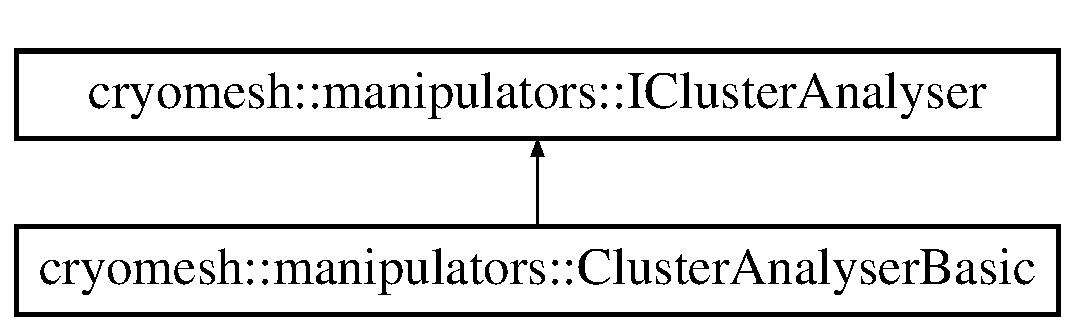
\includegraphics[height=2.000000cm]{classcryomesh_1_1manipulators_1_1ClusterAnalyserBasic}
\end{center}
\end{figure}
\subsection*{\-Public \-Types}
\begin{DoxyCompactItemize}
\item 
enum \hyperlink{classcryomesh_1_1manipulators_1_1IClusterAnalyser_a28a17f8e1363cfb575bacdf213b0781b}{\-Energy\-Variation} \{ \*
\hyperlink{classcryomesh_1_1manipulators_1_1IClusterAnalyser_a28a17f8e1363cfb575bacdf213b0781ba5b6d113aa10f4f70e703a35a39f828d6}{\-N\-O\-N\-E} =  2048, 
\hyperlink{classcryomesh_1_1manipulators_1_1IClusterAnalyser_a28a17f8e1363cfb575bacdf213b0781ba1378201d3fdbeeb653457ffb75488e85}{\-O\-U\-T\-\_\-\-O\-F\-\_\-\-R\-A\-N\-G\-E\-\_\-\-P\-O\-S\-I\-T\-I\-V\-E} =  1024, 
\hyperlink{classcryomesh_1_1manipulators_1_1IClusterAnalyser_a28a17f8e1363cfb575bacdf213b0781baef559139b3fe444fe2b3a24cd8ad0e4d}{\-H\-I\-G\-H\-\_\-\-P\-O\-S\-I\-T\-I\-V\-E} =  512, 
\hyperlink{classcryomesh_1_1manipulators_1_1IClusterAnalyser_a28a17f8e1363cfb575bacdf213b0781baab792b24800c050c84be43dddc08e75c}{\-M\-E\-D\-I\-U\-M\-\_\-\-P\-O\-S\-I\-T\-I\-V\-E} =  256, 
\*
\hyperlink{classcryomesh_1_1manipulators_1_1IClusterAnalyser_a28a17f8e1363cfb575bacdf213b0781ba7d05576fa354d351682eb4fa4f7261e8}{\-S\-M\-A\-L\-L\-\_\-\-P\-O\-S\-I\-T\-I\-V\-E} =  128, 
\hyperlink{classcryomesh_1_1manipulators_1_1IClusterAnalyser_a28a17f8e1363cfb575bacdf213b0781ba27c546877668dfb253e99b8985e4785e}{\-S\-T\-A\-G\-N\-A\-N\-T\-\_\-\-P\-O\-S\-I\-T\-I\-V\-E} =  64, 
\hyperlink{classcryomesh_1_1manipulators_1_1IClusterAnalyser_a28a17f8e1363cfb575bacdf213b0781bae3634dc08cf07554af474b718a1e6b1a}{\-Z\-E\-R\-O} =  32, 
\hyperlink{classcryomesh_1_1manipulators_1_1IClusterAnalyser_a28a17f8e1363cfb575bacdf213b0781bae2174fd5cb8c0db340ffd78804b56947}{\-S\-T\-A\-G\-N\-A\-N\-T\-\_\-\-N\-E\-G\-A\-T\-I\-V\-E} =  16, 
\*
\hyperlink{classcryomesh_1_1manipulators_1_1IClusterAnalyser_a28a17f8e1363cfb575bacdf213b0781bafab77593c2979a49443331f74ed2ba3b}{\-S\-M\-A\-L\-L\-\_\-\-N\-E\-G\-A\-T\-I\-V\-E} =  8, 
\hyperlink{classcryomesh_1_1manipulators_1_1IClusterAnalyser_a28a17f8e1363cfb575bacdf213b0781ba745d3d50f982c9db34f6b55d589ab24c}{\-M\-E\-D\-I\-U\-M\-\_\-\-N\-E\-G\-A\-T\-I\-V\-E} =  4, 
\hyperlink{classcryomesh_1_1manipulators_1_1IClusterAnalyser_a28a17f8e1363cfb575bacdf213b0781bac5cc71ffb113077fb2d67cafb98210e0}{\-H\-I\-G\-H\-\_\-\-N\-E\-G\-A\-T\-I\-V\-E} =  2, 
\hyperlink{classcryomesh_1_1manipulators_1_1IClusterAnalyser_a28a17f8e1363cfb575bacdf213b0781ba531a3f899bfdad545563f019093505c8}{\-O\-U\-T\-\_\-\-O\-F\-\_\-\-R\-A\-N\-G\-E\-\_\-\-N\-E\-G\-A\-T\-I\-V\-E} =  1
 \}
\end{DoxyCompactItemize}
\subsection*{\-Public \-Member \-Functions}
\begin{DoxyCompactItemize}
\item 
\hyperlink{classcryomesh_1_1manipulators_1_1ClusterAnalyserBasic_a66208b2a0fb140dd61b32f2ed0c7769a}{\-Cluster\-Analyser\-Basic} (const \hyperlink{classcryomesh_1_1manipulators_1_1ClusterArchitect}{\-Cluster\-Architect} \&ca)
\item 
virtual \hyperlink{classcryomesh_1_1manipulators_1_1ClusterAnalyserBasic_a6b580c3b0b28b0d9b56132aebe5c72ae}{$\sim$\-Cluster\-Analyser\-Basic} ()
\item 
virtual \hyperlink{classcryomesh_1_1manipulators_1_1ClusterAnalysisData}{\-Cluster\-Analysis\-Data} \hyperlink{classcryomesh_1_1manipulators_1_1ClusterAnalyserBasic_ad98be2e316548236479ce5da459d530b}{analyse\-Cluster} (const \hyperlink{classcryomesh_1_1structures_1_1Cluster}{structures\-::\-Cluster} \&cluster, const std\-::map$<$ int, std\-::list$<$ \hyperlink{classcryomesh_1_1manipulators_1_1ClusterAnalysisData}{\-Cluster\-Analysis\-Data} $>$ $>$ \&histories)
\begin{DoxyCompactList}\small\item\em \-Run an analysis on the cluster to decide what action to take on nodes and connections. \end{DoxyCompactList}\item 
virtual \hyperlink{classcryomesh_1_1manipulators_1_1ClusterAnalysisData}{\-Cluster\-Analysis\-Data} \hyperlink{classcryomesh_1_1manipulators_1_1ClusterAnalyserBasic_ab4e344d193d764d0e60aaed87c9770b3}{calculate\-Range\-Energies} (const std\-::list$<$ \hyperlink{classcryomesh_1_1manipulators_1_1ClusterAnalysisData}{\-Cluster\-Analysis\-Data} $>$ \&history) const 
\begin{DoxyCompactList}\small\item\em \-Calculate the range energies stats. \end{DoxyCompactList}\item 
int \hyperlink{classcryomesh_1_1manipulators_1_1ClusterAnalyserBasic_acfcf0391f2856585d76e72abb3cb729a}{get\-Connection\-Creation\-Enabled\-Countdown} () const 
\item 
int \hyperlink{classcryomesh_1_1manipulators_1_1ClusterAnalyserBasic_a6662b6935836b9a01c62834f09cad3b0}{get\-Connection\-Destruction\-Enabled\-Countdown} () const 
\item 
int \hyperlink{classcryomesh_1_1manipulators_1_1ClusterAnalyserBasic_a9a5351e606da405ecadd9c1fc2b02088}{get\-Node\-Creation\-Enabled\-Countdown} () const 
\item 
int \hyperlink{classcryomesh_1_1manipulators_1_1ClusterAnalyserBasic_a313a72ad507f7bf3c614306c46d872aa}{get\-Node\-Destruction\-Enabled\-Countdown} () const 
\item 
void \hyperlink{classcryomesh_1_1manipulators_1_1ClusterAnalyserBasic_ac816c1b7e855dca5f96dcaa56d6b456c}{set\-Connection\-Destruction\-Enabled\-Countdown} (int connection\-Destruction\-Enabled\-Countdown)
\item 
const \hyperlink{structcryomesh_1_1manipulators_1_1IClusterAnalyser_1_1RestructuringCountdown}{\-Restructuring\-Countdown} \& \hyperlink{classcryomesh_1_1manipulators_1_1IClusterAnalyser_af8eb711949e1d69bbe31b564ff9ab340}{get\-Connection\-Restructuring} () const 
\item 
const \hyperlink{structcryomesh_1_1manipulators_1_1IClusterAnalyser_1_1RestructuringCountdown}{\-Restructuring\-Countdown} \& \hyperlink{classcryomesh_1_1manipulators_1_1IClusterAnalyser_a72da7d8f63441671b8ebd1f4cd994347}{get\-Node\-Restructuring} () const 
\end{DoxyCompactItemize}
\subsection*{\-Protected \-Member \-Functions}
\begin{DoxyCompactItemize}
\item 
virtual \hyperlink{structcryomesh_1_1manipulators_1_1IClusterAnalyser_1_1EnergyVariationWeightingMap}{\-Energy\-Variation\-Weighting\-Map} \hyperlink{classcryomesh_1_1manipulators_1_1ClusterAnalyserBasic_a8870233415221b9c971a30452fb9452a}{get\-Energy\-Variation\-Map} (const double energy\-\_\-input, double range) const 
\end{DoxyCompactItemize}
\subsection*{\-Protected \-Attributes}
\begin{DoxyCompactItemize}
\item 
\hyperlink{structcryomesh_1_1manipulators_1_1IClusterAnalyser_1_1RestructuringCountdown}{\-Restructuring\-Countdown} \hyperlink{classcryomesh_1_1manipulators_1_1IClusterAnalyser_a78d90b9829e4188ded3d94da49c6887a}{node\-Restructuring}
\item 
\hyperlink{structcryomesh_1_1manipulators_1_1IClusterAnalyser_1_1RestructuringCountdown}{\-Restructuring\-Countdown} \hyperlink{classcryomesh_1_1manipulators_1_1IClusterAnalyser_ae0442c245ec17e22d51ffd05c3a2f86e}{connection\-Restructuring}
\end{DoxyCompactItemize}
\subsection*{\-Private \-Attributes}
\begin{DoxyCompactItemize}
\item 
const \hyperlink{classcryomesh_1_1manipulators_1_1ClusterArchitect}{\-Cluster\-Architect} \& \hyperlink{classcryomesh_1_1manipulators_1_1ClusterAnalyserBasic_a680e33ec96d335a5ff84b4398a17ba07}{cluster\-Architect}
\end{DoxyCompactItemize}


\subsection{\-Detailed \-Description}


\-Definition at line 18 of file \-Cluster\-Analyser\-Basic.\-h.



\subsection{\-Member \-Enumeration \-Documentation}
\hypertarget{classcryomesh_1_1manipulators_1_1IClusterAnalyser_a28a17f8e1363cfb575bacdf213b0781b}{\index{cryomesh\-::manipulators\-::\-Cluster\-Analyser\-Basic@{cryomesh\-::manipulators\-::\-Cluster\-Analyser\-Basic}!\-Energy\-Variation@{\-Energy\-Variation}}
\index{\-Energy\-Variation@{\-Energy\-Variation}!cryomesh::manipulators::ClusterAnalyserBasic@{cryomesh\-::manipulators\-::\-Cluster\-Analyser\-Basic}}
\subsubsection[{\-Energy\-Variation}]{\setlength{\rightskip}{0pt plus 5cm}enum {\bf cryomesh\-::manipulators\-::\-I\-Cluster\-Analyser\-::\-Energy\-Variation}\hspace{0.3cm}{\ttfamily  \mbox{[}inherited\mbox{]}}}}\label{classcryomesh_1_1manipulators_1_1IClusterAnalyser_a28a17f8e1363cfb575bacdf213b0781b}
\begin{Desc}
\item[\-Enumerator\-: ]\par
\begin{description}
\index{\-N\-O\-N\-E@{\-N\-O\-N\-E}!cryomesh\-::manipulators\-::\-Cluster\-Analyser\-Basic@{cryomesh\-::manipulators\-::\-Cluster\-Analyser\-Basic}}\index{cryomesh\-::manipulators\-::\-Cluster\-Analyser\-Basic@{cryomesh\-::manipulators\-::\-Cluster\-Analyser\-Basic}!\-N\-O\-N\-E@{\-N\-O\-N\-E}}\item[{\em 
\hypertarget{classcryomesh_1_1manipulators_1_1IClusterAnalyser_a28a17f8e1363cfb575bacdf213b0781ba5b6d113aa10f4f70e703a35a39f828d6}{\-N\-O\-N\-E}\label{classcryomesh_1_1manipulators_1_1IClusterAnalyser_a28a17f8e1363cfb575bacdf213b0781ba5b6d113aa10f4f70e703a35a39f828d6}
}]\index{\-O\-U\-T\-\_\-\-O\-F\-\_\-\-R\-A\-N\-G\-E\-\_\-\-P\-O\-S\-I\-T\-I\-V\-E@{\-O\-U\-T\-\_\-\-O\-F\-\_\-\-R\-A\-N\-G\-E\-\_\-\-P\-O\-S\-I\-T\-I\-V\-E}!cryomesh\-::manipulators\-::\-Cluster\-Analyser\-Basic@{cryomesh\-::manipulators\-::\-Cluster\-Analyser\-Basic}}\index{cryomesh\-::manipulators\-::\-Cluster\-Analyser\-Basic@{cryomesh\-::manipulators\-::\-Cluster\-Analyser\-Basic}!\-O\-U\-T\-\_\-\-O\-F\-\_\-\-R\-A\-N\-G\-E\-\_\-\-P\-O\-S\-I\-T\-I\-V\-E@{\-O\-U\-T\-\_\-\-O\-F\-\_\-\-R\-A\-N\-G\-E\-\_\-\-P\-O\-S\-I\-T\-I\-V\-E}}\item[{\em 
\hypertarget{classcryomesh_1_1manipulators_1_1IClusterAnalyser_a28a17f8e1363cfb575bacdf213b0781ba1378201d3fdbeeb653457ffb75488e85}{\-O\-U\-T\-\_\-\-O\-F\-\_\-\-R\-A\-N\-G\-E\-\_\-\-P\-O\-S\-I\-T\-I\-V\-E}\label{classcryomesh_1_1manipulators_1_1IClusterAnalyser_a28a17f8e1363cfb575bacdf213b0781ba1378201d3fdbeeb653457ffb75488e85}
}]\index{\-H\-I\-G\-H\-\_\-\-P\-O\-S\-I\-T\-I\-V\-E@{\-H\-I\-G\-H\-\_\-\-P\-O\-S\-I\-T\-I\-V\-E}!cryomesh\-::manipulators\-::\-Cluster\-Analyser\-Basic@{cryomesh\-::manipulators\-::\-Cluster\-Analyser\-Basic}}\index{cryomesh\-::manipulators\-::\-Cluster\-Analyser\-Basic@{cryomesh\-::manipulators\-::\-Cluster\-Analyser\-Basic}!\-H\-I\-G\-H\-\_\-\-P\-O\-S\-I\-T\-I\-V\-E@{\-H\-I\-G\-H\-\_\-\-P\-O\-S\-I\-T\-I\-V\-E}}\item[{\em 
\hypertarget{classcryomesh_1_1manipulators_1_1IClusterAnalyser_a28a17f8e1363cfb575bacdf213b0781baef559139b3fe444fe2b3a24cd8ad0e4d}{\-H\-I\-G\-H\-\_\-\-P\-O\-S\-I\-T\-I\-V\-E}\label{classcryomesh_1_1manipulators_1_1IClusterAnalyser_a28a17f8e1363cfb575bacdf213b0781baef559139b3fe444fe2b3a24cd8ad0e4d}
}]\index{\-M\-E\-D\-I\-U\-M\-\_\-\-P\-O\-S\-I\-T\-I\-V\-E@{\-M\-E\-D\-I\-U\-M\-\_\-\-P\-O\-S\-I\-T\-I\-V\-E}!cryomesh\-::manipulators\-::\-Cluster\-Analyser\-Basic@{cryomesh\-::manipulators\-::\-Cluster\-Analyser\-Basic}}\index{cryomesh\-::manipulators\-::\-Cluster\-Analyser\-Basic@{cryomesh\-::manipulators\-::\-Cluster\-Analyser\-Basic}!\-M\-E\-D\-I\-U\-M\-\_\-\-P\-O\-S\-I\-T\-I\-V\-E@{\-M\-E\-D\-I\-U\-M\-\_\-\-P\-O\-S\-I\-T\-I\-V\-E}}\item[{\em 
\hypertarget{classcryomesh_1_1manipulators_1_1IClusterAnalyser_a28a17f8e1363cfb575bacdf213b0781baab792b24800c050c84be43dddc08e75c}{\-M\-E\-D\-I\-U\-M\-\_\-\-P\-O\-S\-I\-T\-I\-V\-E}\label{classcryomesh_1_1manipulators_1_1IClusterAnalyser_a28a17f8e1363cfb575bacdf213b0781baab792b24800c050c84be43dddc08e75c}
}]\index{\-S\-M\-A\-L\-L\-\_\-\-P\-O\-S\-I\-T\-I\-V\-E@{\-S\-M\-A\-L\-L\-\_\-\-P\-O\-S\-I\-T\-I\-V\-E}!cryomesh\-::manipulators\-::\-Cluster\-Analyser\-Basic@{cryomesh\-::manipulators\-::\-Cluster\-Analyser\-Basic}}\index{cryomesh\-::manipulators\-::\-Cluster\-Analyser\-Basic@{cryomesh\-::manipulators\-::\-Cluster\-Analyser\-Basic}!\-S\-M\-A\-L\-L\-\_\-\-P\-O\-S\-I\-T\-I\-V\-E@{\-S\-M\-A\-L\-L\-\_\-\-P\-O\-S\-I\-T\-I\-V\-E}}\item[{\em 
\hypertarget{classcryomesh_1_1manipulators_1_1IClusterAnalyser_a28a17f8e1363cfb575bacdf213b0781ba7d05576fa354d351682eb4fa4f7261e8}{\-S\-M\-A\-L\-L\-\_\-\-P\-O\-S\-I\-T\-I\-V\-E}\label{classcryomesh_1_1manipulators_1_1IClusterAnalyser_a28a17f8e1363cfb575bacdf213b0781ba7d05576fa354d351682eb4fa4f7261e8}
}]\index{\-S\-T\-A\-G\-N\-A\-N\-T\-\_\-\-P\-O\-S\-I\-T\-I\-V\-E@{\-S\-T\-A\-G\-N\-A\-N\-T\-\_\-\-P\-O\-S\-I\-T\-I\-V\-E}!cryomesh\-::manipulators\-::\-Cluster\-Analyser\-Basic@{cryomesh\-::manipulators\-::\-Cluster\-Analyser\-Basic}}\index{cryomesh\-::manipulators\-::\-Cluster\-Analyser\-Basic@{cryomesh\-::manipulators\-::\-Cluster\-Analyser\-Basic}!\-S\-T\-A\-G\-N\-A\-N\-T\-\_\-\-P\-O\-S\-I\-T\-I\-V\-E@{\-S\-T\-A\-G\-N\-A\-N\-T\-\_\-\-P\-O\-S\-I\-T\-I\-V\-E}}\item[{\em 
\hypertarget{classcryomesh_1_1manipulators_1_1IClusterAnalyser_a28a17f8e1363cfb575bacdf213b0781ba27c546877668dfb253e99b8985e4785e}{\-S\-T\-A\-G\-N\-A\-N\-T\-\_\-\-P\-O\-S\-I\-T\-I\-V\-E}\label{classcryomesh_1_1manipulators_1_1IClusterAnalyser_a28a17f8e1363cfb575bacdf213b0781ba27c546877668dfb253e99b8985e4785e}
}]\index{\-Z\-E\-R\-O@{\-Z\-E\-R\-O}!cryomesh\-::manipulators\-::\-Cluster\-Analyser\-Basic@{cryomesh\-::manipulators\-::\-Cluster\-Analyser\-Basic}}\index{cryomesh\-::manipulators\-::\-Cluster\-Analyser\-Basic@{cryomesh\-::manipulators\-::\-Cluster\-Analyser\-Basic}!\-Z\-E\-R\-O@{\-Z\-E\-R\-O}}\item[{\em 
\hypertarget{classcryomesh_1_1manipulators_1_1IClusterAnalyser_a28a17f8e1363cfb575bacdf213b0781bae3634dc08cf07554af474b718a1e6b1a}{\-Z\-E\-R\-O}\label{classcryomesh_1_1manipulators_1_1IClusterAnalyser_a28a17f8e1363cfb575bacdf213b0781bae3634dc08cf07554af474b718a1e6b1a}
}]\index{\-S\-T\-A\-G\-N\-A\-N\-T\-\_\-\-N\-E\-G\-A\-T\-I\-V\-E@{\-S\-T\-A\-G\-N\-A\-N\-T\-\_\-\-N\-E\-G\-A\-T\-I\-V\-E}!cryomesh\-::manipulators\-::\-Cluster\-Analyser\-Basic@{cryomesh\-::manipulators\-::\-Cluster\-Analyser\-Basic}}\index{cryomesh\-::manipulators\-::\-Cluster\-Analyser\-Basic@{cryomesh\-::manipulators\-::\-Cluster\-Analyser\-Basic}!\-S\-T\-A\-G\-N\-A\-N\-T\-\_\-\-N\-E\-G\-A\-T\-I\-V\-E@{\-S\-T\-A\-G\-N\-A\-N\-T\-\_\-\-N\-E\-G\-A\-T\-I\-V\-E}}\item[{\em 
\hypertarget{classcryomesh_1_1manipulators_1_1IClusterAnalyser_a28a17f8e1363cfb575bacdf213b0781bae2174fd5cb8c0db340ffd78804b56947}{\-S\-T\-A\-G\-N\-A\-N\-T\-\_\-\-N\-E\-G\-A\-T\-I\-V\-E}\label{classcryomesh_1_1manipulators_1_1IClusterAnalyser_a28a17f8e1363cfb575bacdf213b0781bae2174fd5cb8c0db340ffd78804b56947}
}]\index{\-S\-M\-A\-L\-L\-\_\-\-N\-E\-G\-A\-T\-I\-V\-E@{\-S\-M\-A\-L\-L\-\_\-\-N\-E\-G\-A\-T\-I\-V\-E}!cryomesh\-::manipulators\-::\-Cluster\-Analyser\-Basic@{cryomesh\-::manipulators\-::\-Cluster\-Analyser\-Basic}}\index{cryomesh\-::manipulators\-::\-Cluster\-Analyser\-Basic@{cryomesh\-::manipulators\-::\-Cluster\-Analyser\-Basic}!\-S\-M\-A\-L\-L\-\_\-\-N\-E\-G\-A\-T\-I\-V\-E@{\-S\-M\-A\-L\-L\-\_\-\-N\-E\-G\-A\-T\-I\-V\-E}}\item[{\em 
\hypertarget{classcryomesh_1_1manipulators_1_1IClusterAnalyser_a28a17f8e1363cfb575bacdf213b0781bafab77593c2979a49443331f74ed2ba3b}{\-S\-M\-A\-L\-L\-\_\-\-N\-E\-G\-A\-T\-I\-V\-E}\label{classcryomesh_1_1manipulators_1_1IClusterAnalyser_a28a17f8e1363cfb575bacdf213b0781bafab77593c2979a49443331f74ed2ba3b}
}]\index{\-M\-E\-D\-I\-U\-M\-\_\-\-N\-E\-G\-A\-T\-I\-V\-E@{\-M\-E\-D\-I\-U\-M\-\_\-\-N\-E\-G\-A\-T\-I\-V\-E}!cryomesh\-::manipulators\-::\-Cluster\-Analyser\-Basic@{cryomesh\-::manipulators\-::\-Cluster\-Analyser\-Basic}}\index{cryomesh\-::manipulators\-::\-Cluster\-Analyser\-Basic@{cryomesh\-::manipulators\-::\-Cluster\-Analyser\-Basic}!\-M\-E\-D\-I\-U\-M\-\_\-\-N\-E\-G\-A\-T\-I\-V\-E@{\-M\-E\-D\-I\-U\-M\-\_\-\-N\-E\-G\-A\-T\-I\-V\-E}}\item[{\em 
\hypertarget{classcryomesh_1_1manipulators_1_1IClusterAnalyser_a28a17f8e1363cfb575bacdf213b0781ba745d3d50f982c9db34f6b55d589ab24c}{\-M\-E\-D\-I\-U\-M\-\_\-\-N\-E\-G\-A\-T\-I\-V\-E}\label{classcryomesh_1_1manipulators_1_1IClusterAnalyser_a28a17f8e1363cfb575bacdf213b0781ba745d3d50f982c9db34f6b55d589ab24c}
}]\index{\-H\-I\-G\-H\-\_\-\-N\-E\-G\-A\-T\-I\-V\-E@{\-H\-I\-G\-H\-\_\-\-N\-E\-G\-A\-T\-I\-V\-E}!cryomesh\-::manipulators\-::\-Cluster\-Analyser\-Basic@{cryomesh\-::manipulators\-::\-Cluster\-Analyser\-Basic}}\index{cryomesh\-::manipulators\-::\-Cluster\-Analyser\-Basic@{cryomesh\-::manipulators\-::\-Cluster\-Analyser\-Basic}!\-H\-I\-G\-H\-\_\-\-N\-E\-G\-A\-T\-I\-V\-E@{\-H\-I\-G\-H\-\_\-\-N\-E\-G\-A\-T\-I\-V\-E}}\item[{\em 
\hypertarget{classcryomesh_1_1manipulators_1_1IClusterAnalyser_a28a17f8e1363cfb575bacdf213b0781bac5cc71ffb113077fb2d67cafb98210e0}{\-H\-I\-G\-H\-\_\-\-N\-E\-G\-A\-T\-I\-V\-E}\label{classcryomesh_1_1manipulators_1_1IClusterAnalyser_a28a17f8e1363cfb575bacdf213b0781bac5cc71ffb113077fb2d67cafb98210e0}
}]\index{\-O\-U\-T\-\_\-\-O\-F\-\_\-\-R\-A\-N\-G\-E\-\_\-\-N\-E\-G\-A\-T\-I\-V\-E@{\-O\-U\-T\-\_\-\-O\-F\-\_\-\-R\-A\-N\-G\-E\-\_\-\-N\-E\-G\-A\-T\-I\-V\-E}!cryomesh\-::manipulators\-::\-Cluster\-Analyser\-Basic@{cryomesh\-::manipulators\-::\-Cluster\-Analyser\-Basic}}\index{cryomesh\-::manipulators\-::\-Cluster\-Analyser\-Basic@{cryomesh\-::manipulators\-::\-Cluster\-Analyser\-Basic}!\-O\-U\-T\-\_\-\-O\-F\-\_\-\-R\-A\-N\-G\-E\-\_\-\-N\-E\-G\-A\-T\-I\-V\-E@{\-O\-U\-T\-\_\-\-O\-F\-\_\-\-R\-A\-N\-G\-E\-\_\-\-N\-E\-G\-A\-T\-I\-V\-E}}\item[{\em 
\hypertarget{classcryomesh_1_1manipulators_1_1IClusterAnalyser_a28a17f8e1363cfb575bacdf213b0781ba531a3f899bfdad545563f019093505c8}{\-O\-U\-T\-\_\-\-O\-F\-\_\-\-R\-A\-N\-G\-E\-\_\-\-N\-E\-G\-A\-T\-I\-V\-E}\label{classcryomesh_1_1manipulators_1_1IClusterAnalyser_a28a17f8e1363cfb575bacdf213b0781ba531a3f899bfdad545563f019093505c8}
}]\end{description}
\end{Desc}



\-Definition at line 136 of file \-I\-Cluster\-Analyser.\-h.



\subsection{\-Constructor \& \-Destructor \-Documentation}
\hypertarget{classcryomesh_1_1manipulators_1_1ClusterAnalyserBasic_a66208b2a0fb140dd61b32f2ed0c7769a}{\index{cryomesh\-::manipulators\-::\-Cluster\-Analyser\-Basic@{cryomesh\-::manipulators\-::\-Cluster\-Analyser\-Basic}!\-Cluster\-Analyser\-Basic@{\-Cluster\-Analyser\-Basic}}
\index{\-Cluster\-Analyser\-Basic@{\-Cluster\-Analyser\-Basic}!cryomesh::manipulators::ClusterAnalyserBasic@{cryomesh\-::manipulators\-::\-Cluster\-Analyser\-Basic}}
\subsubsection[{\-Cluster\-Analyser\-Basic}]{\setlength{\rightskip}{0pt plus 5cm}{\bf cryomesh\-::manipulators\-::\-Cluster\-Analyser\-Basic\-::\-Cluster\-Analyser\-Basic} (
\begin{DoxyParamCaption}
\item[{const {\bf \-Cluster\-Architect} \&}]{ca}
\end{DoxyParamCaption}
)}}\label{classcryomesh_1_1manipulators_1_1ClusterAnalyserBasic_a66208b2a0fb140dd61b32f2ed0c7769a}


\-Definition at line 16 of file \-Cluster\-Analyser\-Basic.\-cpp.

\hypertarget{classcryomesh_1_1manipulators_1_1ClusterAnalyserBasic_a6b580c3b0b28b0d9b56132aebe5c72ae}{\index{cryomesh\-::manipulators\-::\-Cluster\-Analyser\-Basic@{cryomesh\-::manipulators\-::\-Cluster\-Analyser\-Basic}!$\sim$\-Cluster\-Analyser\-Basic@{$\sim$\-Cluster\-Analyser\-Basic}}
\index{$\sim$\-Cluster\-Analyser\-Basic@{$\sim$\-Cluster\-Analyser\-Basic}!cryomesh::manipulators::ClusterAnalyserBasic@{cryomesh\-::manipulators\-::\-Cluster\-Analyser\-Basic}}
\subsubsection[{$\sim$\-Cluster\-Analyser\-Basic}]{\setlength{\rightskip}{0pt plus 5cm}{\bf cryomesh\-::manipulators\-::\-Cluster\-Analyser\-Basic\-::$\sim$\-Cluster\-Analyser\-Basic} (
\begin{DoxyParamCaption}
{}
\end{DoxyParamCaption}
)\hspace{0.3cm}{\ttfamily  \mbox{[}virtual\mbox{]}}}}\label{classcryomesh_1_1manipulators_1_1ClusterAnalyserBasic_a6b580c3b0b28b0d9b56132aebe5c72ae}


\-Definition at line 20 of file \-Cluster\-Analyser\-Basic.\-cpp.



\subsection{\-Member \-Function \-Documentation}
\hypertarget{classcryomesh_1_1manipulators_1_1ClusterAnalyserBasic_ad98be2e316548236479ce5da459d530b}{\index{cryomesh\-::manipulators\-::\-Cluster\-Analyser\-Basic@{cryomesh\-::manipulators\-::\-Cluster\-Analyser\-Basic}!analyse\-Cluster@{analyse\-Cluster}}
\index{analyse\-Cluster@{analyse\-Cluster}!cryomesh::manipulators::ClusterAnalyserBasic@{cryomesh\-::manipulators\-::\-Cluster\-Analyser\-Basic}}
\subsubsection[{analyse\-Cluster}]{\setlength{\rightskip}{0pt plus 5cm}{\bf \-Cluster\-Analysis\-Data} {\bf cryomesh\-::manipulators\-::\-Cluster\-Analyser\-Basic\-::analyse\-Cluster} (
\begin{DoxyParamCaption}
\item[{const {\bf structures\-::\-Cluster} \&}]{cluster, }
\item[{const std\-::map$<$ int, std\-::list$<$ {\bf \-Cluster\-Analysis\-Data} $>$ $>$ \&}]{histories}
\end{DoxyParamCaption}
)\hspace{0.3cm}{\ttfamily  \mbox{[}virtual\mbox{]}}}}\label{classcryomesh_1_1manipulators_1_1ClusterAnalyserBasic_ad98be2e316548236479ce5da459d530b}


\-Run an analysis on the cluster to decide what action to take on nodes and connections. 


\begin{DoxyParams}{\-Parameters}
{\em const} & \hyperlink{classcryomesh_1_1structures_1_1Cluster}{structures\-::\-Cluster} \& \-The cluster to analyse \\
\hline
{\em const} & std\-::list$<$\-Cluster\-Analysis\-Data$>$ \-The historical analysis data to use\\
\hline
\end{DoxyParams}
\begin{DoxyReturn}{\-Returns}
\hyperlink{classcryomesh_1_1manipulators_1_1ClusterAnalysisData}{\-Cluster\-Analysis\-Data} \-The reulting analytical data 
\end{DoxyReturn}


\-Implements \hyperlink{classcryomesh_1_1manipulators_1_1IClusterAnalyser_a0b8594c4b41ed14d5a94d191d1ab11fd}{cryomesh\-::manipulators\-::\-I\-Cluster\-Analyser}.



\-Definition at line 23 of file \-Cluster\-Analyser\-Basic.\-cpp.



\-References calculate\-Range\-Energies(), cluster\-Architect, cryomesh\-::manipulators\-::\-I\-Cluster\-Analyser\-::connection\-Restructuring, cryomesh\-::manipulators\-::\-Cluster\-Analysis\-Data\-::\-Range\-Energy\-::energy\-Fraction, cryomesh\-::manipulators\-::\-Cluster\-Analysis\-Data\-::get\-Cluster\-Range\-Energy(), cryomesh\-::structures\-::\-Cluster\-::get\-Connection\-Map(), cryomesh\-::structures\-::\-Cluster\-::get\-Energy(), get\-Energy\-Variation\-Map(), cryomesh\-::manipulators\-::\-Cluster\-Architect\-::get\-History\-Stepping\-Factor(), cryomesh\-::structures\-::\-Cluster\-::get\-Max\-Energy\-Fraction(), cryomesh\-::manipulators\-::\-Cluster\-Architect\-::get\-Max\-History\-Size(), cryomesh\-::structures\-::\-Cluster\-::get\-Node\-Map(), cryomesh\-::manipulators\-::\-I\-Cluster\-Analyser\-::\-H\-I\-G\-H\-\_\-\-N\-E\-G\-A\-T\-I\-V\-E, cryomesh\-::manipulators\-::\-I\-Cluster\-Analyser\-::\-Restructuring\-Countdown\-::is\-Any\-Long\-Restructuring\-Enabled(), cryomesh\-::manipulators\-::\-I\-Cluster\-Analyser\-::\-Restructuring\-Countdown\-::is\-Any\-Medium\-Restructuring\-Enabled(), cryomesh\-::manipulators\-::\-I\-Cluster\-Analyser\-::\-Restructuring\-Countdown\-::is\-Any\-Restructuring\-Enabled(), cryomesh\-::manipulators\-::\-I\-Cluster\-Analyser\-::\-M\-E\-D\-I\-U\-M\-\_\-\-N\-E\-G\-A\-T\-I\-V\-E, cryomesh\-::manipulators\-::\-I\-Cluster\-Analyser\-::\-M\-E\-D\-I\-U\-M\-\_\-\-P\-O\-S\-I\-T\-I\-V\-E, cryomesh\-::manipulators\-::\-I\-Cluster\-Analyser\-::node\-Restructuring, cryomesh\-::manipulators\-::\-I\-Cluster\-Analyser\-::\-Restructuring\-Countdown\-::set\-Long\-Countdown(), cryomesh\-::manipulators\-::\-I\-Cluster\-Analyser\-::\-Restructuring\-Countdown\-::set\-Medium\-Countdown(), cryomesh\-::manipulators\-::\-I\-Cluster\-Analyser\-::\-S\-M\-A\-L\-L\-\_\-\-N\-E\-G\-A\-T\-I\-V\-E, cryomesh\-::manipulators\-::\-I\-Cluster\-Analyser\-::\-S\-M\-A\-L\-L\-\_\-\-P\-O\-S\-I\-T\-I\-V\-E, cryomesh\-::manipulators\-::\-I\-Cluster\-Analyser\-::\-S\-T\-A\-G\-N\-A\-N\-T\-\_\-\-N\-E\-G\-A\-T\-I\-V\-E, cryomesh\-::manipulators\-::\-I\-Cluster\-Analyser\-::\-S\-T\-A\-G\-N\-A\-N\-T\-\_\-\-P\-O\-S\-I\-T\-I\-V\-E, and cryomesh\-::manipulators\-::\-I\-Cluster\-Analyser\-::\-Energy\-Variation\-Weighting\-Map\-::variation\-Map.

\hypertarget{classcryomesh_1_1manipulators_1_1ClusterAnalyserBasic_ab4e344d193d764d0e60aaed87c9770b3}{\index{cryomesh\-::manipulators\-::\-Cluster\-Analyser\-Basic@{cryomesh\-::manipulators\-::\-Cluster\-Analyser\-Basic}!calculate\-Range\-Energies@{calculate\-Range\-Energies}}
\index{calculate\-Range\-Energies@{calculate\-Range\-Energies}!cryomesh::manipulators::ClusterAnalyserBasic@{cryomesh\-::manipulators\-::\-Cluster\-Analyser\-Basic}}
\subsubsection[{calculate\-Range\-Energies}]{\setlength{\rightskip}{0pt plus 5cm}{\bf \-Cluster\-Analysis\-Data} {\bf cryomesh\-::manipulators\-::\-Cluster\-Analyser\-Basic\-::calculate\-Range\-Energies} (
\begin{DoxyParamCaption}
\item[{const std\-::list$<$ {\bf \-Cluster\-Analysis\-Data} $>$ \&}]{history}
\end{DoxyParamCaption}
) const\hspace{0.3cm}{\ttfamily  \mbox{[}virtual\mbox{]}}}}\label{classcryomesh_1_1manipulators_1_1ClusterAnalyserBasic_ab4e344d193d764d0e60aaed87c9770b3}


\-Calculate the range energies stats. 


\begin{DoxyParams}{\-Parameters}
{\em const} & std\-::list$<$\-Cluster\-Analysis\-Data$>$ \& \-The history range to work with\\
\hline
\end{DoxyParams}
\begin{DoxyReturn}{\-Returns}
\hyperlink{classcryomesh_1_1manipulators_1_1ClusterAnalysisData}{\-Cluster\-Analysis\-Data} \-The resulting cluster analysis data 
\end{DoxyReturn}


\-Implements \hyperlink{classcryomesh_1_1manipulators_1_1IClusterAnalyser_a1f666c2ccf0a6564510c8b4f062e2e21}{cryomesh\-::manipulators\-::\-I\-Cluster\-Analyser}.



\-Definition at line 252 of file \-Cluster\-Analyser\-Basic.\-cpp.



\-References cryomesh\-::manipulators\-::\-Cluster\-Analysis\-Data\-::get\-Cluster\-Range\-Energy(), cryomesh\-::manipulators\-::\-Cluster\-Analysis\-Data\-::get\-Connection\-Creation\-Weight(), cryomesh\-::manipulators\-::\-Cluster\-Analysis\-Data\-::get\-Connection\-Destruction\-Weight(), cryomesh\-::manipulators\-::\-Cluster\-Analysis\-Data\-::get\-Connections\-To\-Create(), cryomesh\-::manipulators\-::\-Cluster\-Analysis\-Data\-::get\-Connections\-To\-Destroy(), cryomesh\-::manipulators\-::\-Cluster\-Analysis\-Data\-::get\-Node\-Creation\-Weight(), cryomesh\-::manipulators\-::\-Cluster\-Analysis\-Data\-::get\-Node\-Destruction\-Weight(), cryomesh\-::manipulators\-::\-Cluster\-Analysis\-Data\-::get\-Nodes\-To\-Create(), and cryomesh\-::manipulators\-::\-Cluster\-Analysis\-Data\-::get\-Nodes\-To\-Destroy().



\-Referenced by analyse\-Cluster().

\hypertarget{classcryomesh_1_1manipulators_1_1ClusterAnalyserBasic_acfcf0391f2856585d76e72abb3cb729a}{\index{cryomesh\-::manipulators\-::\-Cluster\-Analyser\-Basic@{cryomesh\-::manipulators\-::\-Cluster\-Analyser\-Basic}!get\-Connection\-Creation\-Enabled\-Countdown@{get\-Connection\-Creation\-Enabled\-Countdown}}
\index{get\-Connection\-Creation\-Enabled\-Countdown@{get\-Connection\-Creation\-Enabled\-Countdown}!cryomesh::manipulators::ClusterAnalyserBasic@{cryomesh\-::manipulators\-::\-Cluster\-Analyser\-Basic}}
\subsubsection[{get\-Connection\-Creation\-Enabled\-Countdown}]{\setlength{\rightskip}{0pt plus 5cm}int {\bf cryomesh\-::manipulators\-::\-Cluster\-Analyser\-Basic\-::get\-Connection\-Creation\-Enabled\-Countdown} (
\begin{DoxyParamCaption}
{}
\end{DoxyParamCaption}
) const}}\label{classcryomesh_1_1manipulators_1_1ClusterAnalyserBasic_acfcf0391f2856585d76e72abb3cb729a}
\hypertarget{classcryomesh_1_1manipulators_1_1ClusterAnalyserBasic_a6662b6935836b9a01c62834f09cad3b0}{\index{cryomesh\-::manipulators\-::\-Cluster\-Analyser\-Basic@{cryomesh\-::manipulators\-::\-Cluster\-Analyser\-Basic}!get\-Connection\-Destruction\-Enabled\-Countdown@{get\-Connection\-Destruction\-Enabled\-Countdown}}
\index{get\-Connection\-Destruction\-Enabled\-Countdown@{get\-Connection\-Destruction\-Enabled\-Countdown}!cryomesh::manipulators::ClusterAnalyserBasic@{cryomesh\-::manipulators\-::\-Cluster\-Analyser\-Basic}}
\subsubsection[{get\-Connection\-Destruction\-Enabled\-Countdown}]{\setlength{\rightskip}{0pt plus 5cm}int {\bf cryomesh\-::manipulators\-::\-Cluster\-Analyser\-Basic\-::get\-Connection\-Destruction\-Enabled\-Countdown} (
\begin{DoxyParamCaption}
{}
\end{DoxyParamCaption}
) const}}\label{classcryomesh_1_1manipulators_1_1ClusterAnalyserBasic_a6662b6935836b9a01c62834f09cad3b0}
\hypertarget{classcryomesh_1_1manipulators_1_1IClusterAnalyser_af8eb711949e1d69bbe31b564ff9ab340}{\index{cryomesh\-::manipulators\-::\-Cluster\-Analyser\-Basic@{cryomesh\-::manipulators\-::\-Cluster\-Analyser\-Basic}!get\-Connection\-Restructuring@{get\-Connection\-Restructuring}}
\index{get\-Connection\-Restructuring@{get\-Connection\-Restructuring}!cryomesh::manipulators::ClusterAnalyserBasic@{cryomesh\-::manipulators\-::\-Cluster\-Analyser\-Basic}}
\subsubsection[{get\-Connection\-Restructuring}]{\setlength{\rightskip}{0pt plus 5cm}const {\bf \-Restructuring\-Countdown}\& {\bf cryomesh\-::manipulators\-::\-I\-Cluster\-Analyser\-::get\-Connection\-Restructuring} (
\begin{DoxyParamCaption}
{}
\end{DoxyParamCaption}
) const\hspace{0.3cm}{\ttfamily  \mbox{[}inline, inherited\mbox{]}}}}\label{classcryomesh_1_1manipulators_1_1IClusterAnalyser_af8eb711949e1d69bbe31b564ff9ab340}


\-Definition at line 198 of file \-I\-Cluster\-Analyser.\-h.



\-References cryomesh\-::manipulators\-::\-I\-Cluster\-Analyser\-::connection\-Restructuring.

\hypertarget{classcryomesh_1_1manipulators_1_1ClusterAnalyserBasic_a8870233415221b9c971a30452fb9452a}{\index{cryomesh\-::manipulators\-::\-Cluster\-Analyser\-Basic@{cryomesh\-::manipulators\-::\-Cluster\-Analyser\-Basic}!get\-Energy\-Variation\-Map@{get\-Energy\-Variation\-Map}}
\index{get\-Energy\-Variation\-Map@{get\-Energy\-Variation\-Map}!cryomesh::manipulators::ClusterAnalyserBasic@{cryomesh\-::manipulators\-::\-Cluster\-Analyser\-Basic}}
\subsubsection[{get\-Energy\-Variation\-Map}]{\setlength{\rightskip}{0pt plus 5cm}{\bf \-Cluster\-Analyser\-Basic\-::\-Energy\-Variation\-Weighting\-Map} {\bf cryomesh\-::manipulators\-::\-Cluster\-Analyser\-Basic\-::get\-Energy\-Variation\-Map} (
\begin{DoxyParamCaption}
\item[{const double}]{energy\-\_\-input, }
\item[{double}]{range}
\end{DoxyParamCaption}
) const\hspace{0.3cm}{\ttfamily  \mbox{[}protected, virtual\mbox{]}}}}\label{classcryomesh_1_1manipulators_1_1ClusterAnalyserBasic_a8870233415221b9c971a30452fb9452a}


\-Implements \hyperlink{classcryomesh_1_1manipulators_1_1IClusterAnalyser_a27db139b4aa43f0c008de165d2f22f5b}{cryomesh\-::manipulators\-::\-I\-Cluster\-Analyser}.



\-Definition at line 307 of file \-Cluster\-Analyser\-Basic.\-cpp.



\-References cryomesh\-::manipulators\-::\-I\-Cluster\-Analyser\-::\-H\-I\-G\-H\-\_\-\-N\-E\-G\-A\-T\-I\-V\-E, cryomesh\-::manipulators\-::\-I\-Cluster\-Analyser\-::\-H\-I\-G\-H\-\_\-\-P\-O\-S\-I\-T\-I\-V\-E, cryomesh\-::manipulators\-::\-I\-Cluster\-Analyser\-::\-M\-E\-D\-I\-U\-M\-\_\-\-N\-E\-G\-A\-T\-I\-V\-E, cryomesh\-::manipulators\-::\-I\-Cluster\-Analyser\-::\-M\-E\-D\-I\-U\-M\-\_\-\-P\-O\-S\-I\-T\-I\-V\-E, cryomesh\-::manipulators\-::\-I\-Cluster\-Analyser\-::\-O\-U\-T\-\_\-\-O\-F\-\_\-\-R\-A\-N\-G\-E\-\_\-\-N\-E\-G\-A\-T\-I\-V\-E, cryomesh\-::manipulators\-::\-I\-Cluster\-Analyser\-::\-O\-U\-T\-\_\-\-O\-F\-\_\-\-R\-A\-N\-G\-E\-\_\-\-P\-O\-S\-I\-T\-I\-V\-E, cryomesh\-::manipulators\-::\-I\-Cluster\-Analyser\-::\-S\-M\-A\-L\-L\-\_\-\-N\-E\-G\-A\-T\-I\-V\-E, cryomesh\-::manipulators\-::\-I\-Cluster\-Analyser\-::\-S\-M\-A\-L\-L\-\_\-\-P\-O\-S\-I\-T\-I\-V\-E, cryomesh\-::manipulators\-::\-I\-Cluster\-Analyser\-::\-S\-T\-A\-G\-N\-A\-N\-T\-\_\-\-N\-E\-G\-A\-T\-I\-V\-E, cryomesh\-::manipulators\-::\-I\-Cluster\-Analyser\-::\-S\-T\-A\-G\-N\-A\-N\-T\-\_\-\-P\-O\-S\-I\-T\-I\-V\-E, cryomesh\-::manipulators\-::\-I\-Cluster\-Analyser\-::\-Energy\-Variation\-Weighting\-Map\-::variation\-Map, and cryomesh\-::manipulators\-::\-I\-Cluster\-Analyser\-::\-Z\-E\-R\-O.



\-Referenced by analyse\-Cluster().

\hypertarget{classcryomesh_1_1manipulators_1_1ClusterAnalyserBasic_a9a5351e606da405ecadd9c1fc2b02088}{\index{cryomesh\-::manipulators\-::\-Cluster\-Analyser\-Basic@{cryomesh\-::manipulators\-::\-Cluster\-Analyser\-Basic}!get\-Node\-Creation\-Enabled\-Countdown@{get\-Node\-Creation\-Enabled\-Countdown}}
\index{get\-Node\-Creation\-Enabled\-Countdown@{get\-Node\-Creation\-Enabled\-Countdown}!cryomesh::manipulators::ClusterAnalyserBasic@{cryomesh\-::manipulators\-::\-Cluster\-Analyser\-Basic}}
\subsubsection[{get\-Node\-Creation\-Enabled\-Countdown}]{\setlength{\rightskip}{0pt plus 5cm}int {\bf cryomesh\-::manipulators\-::\-Cluster\-Analyser\-Basic\-::get\-Node\-Creation\-Enabled\-Countdown} (
\begin{DoxyParamCaption}
{}
\end{DoxyParamCaption}
) const}}\label{classcryomesh_1_1manipulators_1_1ClusterAnalyserBasic_a9a5351e606da405ecadd9c1fc2b02088}
\hypertarget{classcryomesh_1_1manipulators_1_1ClusterAnalyserBasic_a313a72ad507f7bf3c614306c46d872aa}{\index{cryomesh\-::manipulators\-::\-Cluster\-Analyser\-Basic@{cryomesh\-::manipulators\-::\-Cluster\-Analyser\-Basic}!get\-Node\-Destruction\-Enabled\-Countdown@{get\-Node\-Destruction\-Enabled\-Countdown}}
\index{get\-Node\-Destruction\-Enabled\-Countdown@{get\-Node\-Destruction\-Enabled\-Countdown}!cryomesh::manipulators::ClusterAnalyserBasic@{cryomesh\-::manipulators\-::\-Cluster\-Analyser\-Basic}}
\subsubsection[{get\-Node\-Destruction\-Enabled\-Countdown}]{\setlength{\rightskip}{0pt plus 5cm}int {\bf cryomesh\-::manipulators\-::\-Cluster\-Analyser\-Basic\-::get\-Node\-Destruction\-Enabled\-Countdown} (
\begin{DoxyParamCaption}
{}
\end{DoxyParamCaption}
) const}}\label{classcryomesh_1_1manipulators_1_1ClusterAnalyserBasic_a313a72ad507f7bf3c614306c46d872aa}
\hypertarget{classcryomesh_1_1manipulators_1_1IClusterAnalyser_a72da7d8f63441671b8ebd1f4cd994347}{\index{cryomesh\-::manipulators\-::\-Cluster\-Analyser\-Basic@{cryomesh\-::manipulators\-::\-Cluster\-Analyser\-Basic}!get\-Node\-Restructuring@{get\-Node\-Restructuring}}
\index{get\-Node\-Restructuring@{get\-Node\-Restructuring}!cryomesh::manipulators::ClusterAnalyserBasic@{cryomesh\-::manipulators\-::\-Cluster\-Analyser\-Basic}}
\subsubsection[{get\-Node\-Restructuring}]{\setlength{\rightskip}{0pt plus 5cm}const {\bf \-Restructuring\-Countdown}\& {\bf cryomesh\-::manipulators\-::\-I\-Cluster\-Analyser\-::get\-Node\-Restructuring} (
\begin{DoxyParamCaption}
{}
\end{DoxyParamCaption}
) const\hspace{0.3cm}{\ttfamily  \mbox{[}inline, inherited\mbox{]}}}}\label{classcryomesh_1_1manipulators_1_1IClusterAnalyser_a72da7d8f63441671b8ebd1f4cd994347}


\-Definition at line 201 of file \-I\-Cluster\-Analyser.\-h.



\-References cryomesh\-::manipulators\-::\-I\-Cluster\-Analyser\-::node\-Restructuring.

\hypertarget{classcryomesh_1_1manipulators_1_1ClusterAnalyserBasic_ac816c1b7e855dca5f96dcaa56d6b456c}{\index{cryomesh\-::manipulators\-::\-Cluster\-Analyser\-Basic@{cryomesh\-::manipulators\-::\-Cluster\-Analyser\-Basic}!set\-Connection\-Destruction\-Enabled\-Countdown@{set\-Connection\-Destruction\-Enabled\-Countdown}}
\index{set\-Connection\-Destruction\-Enabled\-Countdown@{set\-Connection\-Destruction\-Enabled\-Countdown}!cryomesh::manipulators::ClusterAnalyserBasic@{cryomesh\-::manipulators\-::\-Cluster\-Analyser\-Basic}}
\subsubsection[{set\-Connection\-Destruction\-Enabled\-Countdown}]{\setlength{\rightskip}{0pt plus 5cm}void {\bf cryomesh\-::manipulators\-::\-Cluster\-Analyser\-Basic\-::set\-Connection\-Destruction\-Enabled\-Countdown} (
\begin{DoxyParamCaption}
\item[{int}]{connection\-Destruction\-Enabled\-Countdown}
\end{DoxyParamCaption}
)}}\label{classcryomesh_1_1manipulators_1_1ClusterAnalyserBasic_ac816c1b7e855dca5f96dcaa56d6b456c}


\subsection{\-Member \-Data \-Documentation}
\hypertarget{classcryomesh_1_1manipulators_1_1ClusterAnalyserBasic_a680e33ec96d335a5ff84b4398a17ba07}{\index{cryomesh\-::manipulators\-::\-Cluster\-Analyser\-Basic@{cryomesh\-::manipulators\-::\-Cluster\-Analyser\-Basic}!cluster\-Architect@{cluster\-Architect}}
\index{cluster\-Architect@{cluster\-Architect}!cryomesh::manipulators::ClusterAnalyserBasic@{cryomesh\-::manipulators\-::\-Cluster\-Analyser\-Basic}}
\subsubsection[{cluster\-Architect}]{\setlength{\rightskip}{0pt plus 5cm}const {\bf \-Cluster\-Architect}\& {\bf cryomesh\-::manipulators\-::\-Cluster\-Analyser\-Basic\-::cluster\-Architect}\hspace{0.3cm}{\ttfamily  \mbox{[}private\mbox{]}}}}\label{classcryomesh_1_1manipulators_1_1ClusterAnalyserBasic_a680e33ec96d335a5ff84b4398a17ba07}


\-Definition at line 36 of file \-Cluster\-Analyser\-Basic.\-h.



\-Referenced by analyse\-Cluster().

\hypertarget{classcryomesh_1_1manipulators_1_1IClusterAnalyser_ae0442c245ec17e22d51ffd05c3a2f86e}{\index{cryomesh\-::manipulators\-::\-Cluster\-Analyser\-Basic@{cryomesh\-::manipulators\-::\-Cluster\-Analyser\-Basic}!connection\-Restructuring@{connection\-Restructuring}}
\index{connection\-Restructuring@{connection\-Restructuring}!cryomesh::manipulators::ClusterAnalyserBasic@{cryomesh\-::manipulators\-::\-Cluster\-Analyser\-Basic}}
\subsubsection[{connection\-Restructuring}]{\setlength{\rightskip}{0pt plus 5cm}{\bf \-Restructuring\-Countdown} {\bf cryomesh\-::manipulators\-::\-I\-Cluster\-Analyser\-::connection\-Restructuring}\hspace{0.3cm}{\ttfamily  \mbox{[}protected, inherited\mbox{]}}}}\label{classcryomesh_1_1manipulators_1_1IClusterAnalyser_ae0442c245ec17e22d51ffd05c3a2f86e}


\-Definition at line 206 of file \-I\-Cluster\-Analyser.\-h.



\-Referenced by analyse\-Cluster(), and cryomesh\-::manipulators\-::\-I\-Cluster\-Analyser\-::get\-Connection\-Restructuring().

\hypertarget{classcryomesh_1_1manipulators_1_1IClusterAnalyser_a78d90b9829e4188ded3d94da49c6887a}{\index{cryomesh\-::manipulators\-::\-Cluster\-Analyser\-Basic@{cryomesh\-::manipulators\-::\-Cluster\-Analyser\-Basic}!node\-Restructuring@{node\-Restructuring}}
\index{node\-Restructuring@{node\-Restructuring}!cryomesh::manipulators::ClusterAnalyserBasic@{cryomesh\-::manipulators\-::\-Cluster\-Analyser\-Basic}}
\subsubsection[{node\-Restructuring}]{\setlength{\rightskip}{0pt plus 5cm}{\bf \-Restructuring\-Countdown} {\bf cryomesh\-::manipulators\-::\-I\-Cluster\-Analyser\-::node\-Restructuring}\hspace{0.3cm}{\ttfamily  \mbox{[}protected, inherited\mbox{]}}}}\label{classcryomesh_1_1manipulators_1_1IClusterAnalyser_a78d90b9829e4188ded3d94da49c6887a}


\-Definition at line 205 of file \-I\-Cluster\-Analyser.\-h.



\-Referenced by analyse\-Cluster(), and cryomesh\-::manipulators\-::\-I\-Cluster\-Analyser\-::get\-Node\-Restructuring().



\-The documentation for this class was generated from the following files\-:\begin{DoxyCompactItemize}
\item 
/home/niall/\-Projects/\-Eclipse/\-C\-P\-P/cryomesh/src/manipulators/\hyperlink{ClusterAnalyserBasic_8h}{\-Cluster\-Analyser\-Basic.\-h}\item 
/home/niall/\-Projects/\-Eclipse/\-C\-P\-P/cryomesh/src/manipulators/\hyperlink{ClusterAnalyserBasic_8cpp}{\-Cluster\-Analyser\-Basic.\-cpp}\end{DoxyCompactItemize}

\hypertarget{classcryomesh_1_1manipulators_1_1ClusterAnalysisData}{\section{cryomesh\-:\-:manipulators\-:\-:\-Cluster\-Analysis\-Data \-Class \-Reference}
\label{classcryomesh_1_1manipulators_1_1ClusterAnalysisData}\index{cryomesh\-::manipulators\-::\-Cluster\-Analysis\-Data@{cryomesh\-::manipulators\-::\-Cluster\-Analysis\-Data}}
}


{\ttfamily \#include $<$\-Cluster\-Analysis\-Data.\-h$>$}

\subsection*{\-Classes}
\begin{DoxyCompactItemize}
\item 
struct \hyperlink{structcryomesh_1_1manipulators_1_1ClusterAnalysisData_1_1RangeEnergy}{\-Range\-Energy}
\begin{DoxyCompactList}\small\item\em \-Struct representing the value extrapolated over a history range. \end{DoxyCompactList}\end{DoxyCompactItemize}
\subsection*{\-Public \-Member \-Functions}
\begin{DoxyCompactItemize}
\item 
\hyperlink{classcryomesh_1_1manipulators_1_1ClusterAnalysisData_a98f5e73167b6c67c2ccaf323d2746eb5}{\-Cluster\-Analysis\-Data} ()
\item 
\hyperlink{classcryomesh_1_1manipulators_1_1ClusterAnalysisData_a3b924bf249e5da2908ba59e523178be0}{\-Cluster\-Analysis\-Data} (\hyperlink{structcryomesh_1_1manipulators_1_1ClusterAnalysisData_1_1RangeEnergy}{\-Range\-Energy} cre)
\item 
\hyperlink{classcryomesh_1_1manipulators_1_1ClusterAnalysisData_a2fa4c1fd92df8f5f84d7574598c44a31}{\-Cluster\-Analysis\-Data} (\hyperlink{structcryomesh_1_1manipulators_1_1ClusterAnalysisData_1_1RangeEnergy}{\-Range\-Energy} \hyperlink{classcryomesh_1_1manipulators_1_1ClusterAnalysisData_a2cc91850c86c1a09509266b639cbacdb}{cluster\-Range\-Energy}, double node\-\_\-creation\-\_\-weight, double node\-\_\-destruction\-\_\-weight, double conn\-\_\-creation\-\_\-weight, double conn\-\_\-destruction\-\_\-weight, int node\-\_\-create, int nodes\-\_\-destroy, int conn\-\_\-create, int conn\-\_\-destroy)
\item 
\hyperlink{classcryomesh_1_1manipulators_1_1ClusterAnalysisData_ac94a5b4dfcba2a089bcb2bb768efc27a}{\-Cluster\-Analysis\-Data} (const \hyperlink{classcryomesh_1_1manipulators_1_1ClusterAnalysisData}{\-Cluster\-Analysis\-Data} \&obj)
\item 
virtual \hyperlink{classcryomesh_1_1manipulators_1_1ClusterAnalysisData_a6a8af77c801c546b8286f7611d63240a}{$\sim$\-Cluster\-Analysis\-Data} ()
\item 
\hyperlink{structcryomesh_1_1manipulators_1_1ClusterAnalysisData_1_1RangeEnergy}{\-Range\-Energy} \hyperlink{classcryomesh_1_1manipulators_1_1ClusterAnalysisData_a671823e8f64d2525f3084e7ab82ce205}{get\-Cluster\-Range\-Energy} () const 
\item 
double \hyperlink{classcryomesh_1_1manipulators_1_1ClusterAnalysisData_a849a5a4bedbf3267883a34695d9fc832}{get\-Node\-Creation\-Weight} () const 
\item 
double \hyperlink{classcryomesh_1_1manipulators_1_1ClusterAnalysisData_a39954c2cfd0bf18ad011f1b637f02b26}{get\-Node\-Destruction\-Weight} () const 
\item 
double \hyperlink{classcryomesh_1_1manipulators_1_1ClusterAnalysisData_a59df774485e384f9706d12085cc1448a}{get\-Connection\-Creation\-Weight} () const 
\item 
double \hyperlink{classcryomesh_1_1manipulators_1_1ClusterAnalysisData_a37ebc1eeb8acca183b93d379c59f0dc6}{get\-Connection\-Destruction\-Weight} () const 
\item 
int \hyperlink{classcryomesh_1_1manipulators_1_1ClusterAnalysisData_a04bbdb34881e7d5a716e6b45b461a330}{get\-Nodes\-To\-Destroy} () const 
\item 
int \hyperlink{classcryomesh_1_1manipulators_1_1ClusterAnalysisData_aedee2369cd1b2a8c934b3fe75b063eaf}{get\-Connections\-To\-Destroy} () const 
\item 
int \hyperlink{classcryomesh_1_1manipulators_1_1ClusterAnalysisData_a89a5f4d7d395f192c9d7809783584608}{get\-Nodes\-To\-Create} () const 
\item 
int \hyperlink{classcryomesh_1_1manipulators_1_1ClusterAnalysisData_adb384db5722ed36e50218b6a99362524}{get\-Connections\-To\-Create} () const 
\item 
void \hyperlink{classcryomesh_1_1manipulators_1_1ClusterAnalysisData_aa1b5e2b36b91959135ed40a1e0393309}{set\-Cluster\-Range\-Energy} (\hyperlink{structcryomesh_1_1manipulators_1_1ClusterAnalysisData_1_1RangeEnergy}{\-Range\-Energy} cluster\-Energy)
\item 
void \hyperlink{classcryomesh_1_1manipulators_1_1ClusterAnalysisData_a4afa9476dc34d1c4230915c135f0f085}{set\-Connection\-Creation\-Weight} (double \hyperlink{classcryomesh_1_1manipulators_1_1ClusterAnalysisData_a25abb815b2869d410c9d32819471d67b}{connection\-Creation\-Weight})
\item 
void \hyperlink{classcryomesh_1_1manipulators_1_1ClusterAnalysisData_aa8370250c00d64878683d0c34663f23a}{set\-Connection\-Destruction\-Weight} (double \hyperlink{classcryomesh_1_1manipulators_1_1ClusterAnalysisData_ac9f1a2eada7f214b62a257067ee7d336}{connection\-Destruction\-Weight})
\item 
void \hyperlink{classcryomesh_1_1manipulators_1_1ClusterAnalysisData_a390b7af8b7aaad30ae2434d3cc38ce34}{set\-Connections\-To\-Create} (int \hyperlink{classcryomesh_1_1manipulators_1_1ClusterAnalysisData_add3ac0cb45a6782d3d92d9d4ea181609}{connections\-To\-Create})
\item 
void \hyperlink{classcryomesh_1_1manipulators_1_1ClusterAnalysisData_a92092f1fc3184708f2360a1f237330c1}{set\-Connections\-To\-Destroy} (int \hyperlink{classcryomesh_1_1manipulators_1_1ClusterAnalysisData_a303e9f1b0de641d8c3f79ff4ad05a9a5}{connections\-To\-Destroy})
\item 
void \hyperlink{classcryomesh_1_1manipulators_1_1ClusterAnalysisData_a41ad78f8918e9898e7c4d08263e631c2}{set\-Node\-Creation\-Weight} (double \hyperlink{classcryomesh_1_1manipulators_1_1ClusterAnalysisData_a135e912ae399505480429e488a163d75}{node\-Creation\-Weight})
\item 
void \hyperlink{classcryomesh_1_1manipulators_1_1ClusterAnalysisData_a6bbc3f1089e480e644517c01e119cc56}{set\-Node\-Destruction\-Weight} (double \hyperlink{classcryomesh_1_1manipulators_1_1ClusterAnalysisData_ace52167d730c5513c9981a7be9a56499}{node\-Destruction\-Weight})
\item 
void \hyperlink{classcryomesh_1_1manipulators_1_1ClusterAnalysisData_a76000e1f7a03c3026f5e0c8c34cb655c}{set\-Nodes\-To\-Create} (int \hyperlink{classcryomesh_1_1manipulators_1_1ClusterAnalysisData_aa7100219ad6f168229ae1bea3b0f4c95}{nodes\-To\-Create})
\item 
void \hyperlink{classcryomesh_1_1manipulators_1_1ClusterAnalysisData_ae42bcf04427d1260b7c4210bff7dc109}{set\-Nodes\-To\-Destroy} (int \hyperlink{classcryomesh_1_1manipulators_1_1ClusterAnalysisData_afcdd6cf5b2a890ed24cce7ddf6855bd8}{nodes\-To\-Destroy})
\end{DoxyCompactItemize}
\subsection*{\-Private \-Attributes}
\begin{DoxyCompactItemize}
\item 
\hyperlink{structcryomesh_1_1manipulators_1_1ClusterAnalysisData_1_1RangeEnergy}{\-Range\-Energy} \hyperlink{classcryomesh_1_1manipulators_1_1ClusterAnalysisData_a2cc91850c86c1a09509266b639cbacdb}{cluster\-Range\-Energy}
\item 
double \hyperlink{classcryomesh_1_1manipulators_1_1ClusterAnalysisData_a135e912ae399505480429e488a163d75}{node\-Creation\-Weight}
\item 
double \hyperlink{classcryomesh_1_1manipulators_1_1ClusterAnalysisData_ace52167d730c5513c9981a7be9a56499}{node\-Destruction\-Weight}
\item 
double \hyperlink{classcryomesh_1_1manipulators_1_1ClusterAnalysisData_a25abb815b2869d410c9d32819471d67b}{connection\-Creation\-Weight}
\item 
double \hyperlink{classcryomesh_1_1manipulators_1_1ClusterAnalysisData_ac9f1a2eada7f214b62a257067ee7d336}{connection\-Destruction\-Weight}
\item 
int \hyperlink{classcryomesh_1_1manipulators_1_1ClusterAnalysisData_aa7100219ad6f168229ae1bea3b0f4c95}{nodes\-To\-Create}
\item 
int \hyperlink{classcryomesh_1_1manipulators_1_1ClusterAnalysisData_afcdd6cf5b2a890ed24cce7ddf6855bd8}{nodes\-To\-Destroy}
\item 
int \hyperlink{classcryomesh_1_1manipulators_1_1ClusterAnalysisData_add3ac0cb45a6782d3d92d9d4ea181609}{connections\-To\-Create}
\item 
int \hyperlink{classcryomesh_1_1manipulators_1_1ClusterAnalysisData_a303e9f1b0de641d8c3f79ff4ad05a9a5}{connections\-To\-Destroy}
\end{DoxyCompactItemize}
\subsection*{\-Friends}
\begin{DoxyCompactItemize}
\item 
std\-::ostream \& \hyperlink{classcryomesh_1_1manipulators_1_1ClusterAnalysisData_ab5e82a523fb5b8d1621b38ce4affa82b}{operator$<$$<$} (std\-::ostream \&os, const \hyperlink{classcryomesh_1_1manipulators_1_1ClusterAnalysisData}{\-Cluster\-Analysis\-Data} \&obj)
\begin{DoxyCompactList}\small\item\em \-To stream operator. \end{DoxyCompactList}\end{DoxyCompactItemize}


\subsection{\-Detailed \-Description}


\-Definition at line 18 of file \-Cluster\-Analysis\-Data.\-h.



\subsection{\-Constructor \& \-Destructor \-Documentation}
\hypertarget{classcryomesh_1_1manipulators_1_1ClusterAnalysisData_a98f5e73167b6c67c2ccaf323d2746eb5}{\index{cryomesh\-::manipulators\-::\-Cluster\-Analysis\-Data@{cryomesh\-::manipulators\-::\-Cluster\-Analysis\-Data}!\-Cluster\-Analysis\-Data@{\-Cluster\-Analysis\-Data}}
\index{\-Cluster\-Analysis\-Data@{\-Cluster\-Analysis\-Data}!cryomesh::manipulators::ClusterAnalysisData@{cryomesh\-::manipulators\-::\-Cluster\-Analysis\-Data}}
\subsubsection[{\-Cluster\-Analysis\-Data}]{\setlength{\rightskip}{0pt plus 5cm}{\bf cryomesh\-::manipulators\-::\-Cluster\-Analysis\-Data\-::\-Cluster\-Analysis\-Data} (
\begin{DoxyParamCaption}
{}
\end{DoxyParamCaption}
)}}\label{classcryomesh_1_1manipulators_1_1ClusterAnalysisData_a98f5e73167b6c67c2ccaf323d2746eb5}


\-Definition at line 13 of file \-Cluster\-Analysis\-Data.\-cpp.

\hypertarget{classcryomesh_1_1manipulators_1_1ClusterAnalysisData_a3b924bf249e5da2908ba59e523178be0}{\index{cryomesh\-::manipulators\-::\-Cluster\-Analysis\-Data@{cryomesh\-::manipulators\-::\-Cluster\-Analysis\-Data}!\-Cluster\-Analysis\-Data@{\-Cluster\-Analysis\-Data}}
\index{\-Cluster\-Analysis\-Data@{\-Cluster\-Analysis\-Data}!cryomesh::manipulators::ClusterAnalysisData@{cryomesh\-::manipulators\-::\-Cluster\-Analysis\-Data}}
\subsubsection[{\-Cluster\-Analysis\-Data}]{\setlength{\rightskip}{0pt plus 5cm}{\bf cryomesh\-::manipulators\-::\-Cluster\-Analysis\-Data\-::\-Cluster\-Analysis\-Data} (
\begin{DoxyParamCaption}
\item[{{\bf \-Range\-Energy}}]{cre}
\end{DoxyParamCaption}
)}}\label{classcryomesh_1_1manipulators_1_1ClusterAnalysisData_a3b924bf249e5da2908ba59e523178be0}


\-Definition at line 17 of file \-Cluster\-Analysis\-Data.\-cpp.

\hypertarget{classcryomesh_1_1manipulators_1_1ClusterAnalysisData_a2fa4c1fd92df8f5f84d7574598c44a31}{\index{cryomesh\-::manipulators\-::\-Cluster\-Analysis\-Data@{cryomesh\-::manipulators\-::\-Cluster\-Analysis\-Data}!\-Cluster\-Analysis\-Data@{\-Cluster\-Analysis\-Data}}
\index{\-Cluster\-Analysis\-Data@{\-Cluster\-Analysis\-Data}!cryomesh::manipulators::ClusterAnalysisData@{cryomesh\-::manipulators\-::\-Cluster\-Analysis\-Data}}
\subsubsection[{\-Cluster\-Analysis\-Data}]{\setlength{\rightskip}{0pt plus 5cm}{\bf cryomesh\-::manipulators\-::\-Cluster\-Analysis\-Data\-::\-Cluster\-Analysis\-Data} (
\begin{DoxyParamCaption}
\item[{{\bf \-Range\-Energy}}]{cluster\-Range\-Energy, }
\item[{double}]{node\-\_\-creation\-\_\-weight, }
\item[{double}]{node\-\_\-destruction\-\_\-weight, }
\item[{double}]{conn\-\_\-creation\-\_\-weight, }
\item[{double}]{conn\-\_\-destruction\-\_\-weight, }
\item[{int}]{node\-\_\-create, }
\item[{int}]{nodes\-\_\-destroy, }
\item[{int}]{conn\-\_\-create, }
\item[{int}]{conn\-\_\-destroy}
\end{DoxyParamCaption}
)}}\label{classcryomesh_1_1manipulators_1_1ClusterAnalysisData_a2fa4c1fd92df8f5f84d7574598c44a31}


\-Definition at line 22 of file \-Cluster\-Analysis\-Data.\-cpp.

\hypertarget{classcryomesh_1_1manipulators_1_1ClusterAnalysisData_ac94a5b4dfcba2a089bcb2bb768efc27a}{\index{cryomesh\-::manipulators\-::\-Cluster\-Analysis\-Data@{cryomesh\-::manipulators\-::\-Cluster\-Analysis\-Data}!\-Cluster\-Analysis\-Data@{\-Cluster\-Analysis\-Data}}
\index{\-Cluster\-Analysis\-Data@{\-Cluster\-Analysis\-Data}!cryomesh::manipulators::ClusterAnalysisData@{cryomesh\-::manipulators\-::\-Cluster\-Analysis\-Data}}
\subsubsection[{\-Cluster\-Analysis\-Data}]{\setlength{\rightskip}{0pt plus 5cm}{\bf cryomesh\-::manipulators\-::\-Cluster\-Analysis\-Data\-::\-Cluster\-Analysis\-Data} (
\begin{DoxyParamCaption}
\item[{const {\bf \-Cluster\-Analysis\-Data} \&}]{obj}
\end{DoxyParamCaption}
)}}\label{classcryomesh_1_1manipulators_1_1ClusterAnalysisData_ac94a5b4dfcba2a089bcb2bb768efc27a}


\-Definition at line 31 of file \-Cluster\-Analysis\-Data.\-cpp.

\hypertarget{classcryomesh_1_1manipulators_1_1ClusterAnalysisData_a6a8af77c801c546b8286f7611d63240a}{\index{cryomesh\-::manipulators\-::\-Cluster\-Analysis\-Data@{cryomesh\-::manipulators\-::\-Cluster\-Analysis\-Data}!$\sim$\-Cluster\-Analysis\-Data@{$\sim$\-Cluster\-Analysis\-Data}}
\index{$\sim$\-Cluster\-Analysis\-Data@{$\sim$\-Cluster\-Analysis\-Data}!cryomesh::manipulators::ClusterAnalysisData@{cryomesh\-::manipulators\-::\-Cluster\-Analysis\-Data}}
\subsubsection[{$\sim$\-Cluster\-Analysis\-Data}]{\setlength{\rightskip}{0pt plus 5cm}{\bf cryomesh\-::manipulators\-::\-Cluster\-Analysis\-Data\-::$\sim$\-Cluster\-Analysis\-Data} (
\begin{DoxyParamCaption}
{}
\end{DoxyParamCaption}
)\hspace{0.3cm}{\ttfamily  \mbox{[}virtual\mbox{]}}}}\label{classcryomesh_1_1manipulators_1_1ClusterAnalysisData_a6a8af77c801c546b8286f7611d63240a}


\-Definition at line 38 of file \-Cluster\-Analysis\-Data.\-cpp.



\subsection{\-Member \-Function \-Documentation}
\hypertarget{classcryomesh_1_1manipulators_1_1ClusterAnalysisData_a671823e8f64d2525f3084e7ab82ce205}{\index{cryomesh\-::manipulators\-::\-Cluster\-Analysis\-Data@{cryomesh\-::manipulators\-::\-Cluster\-Analysis\-Data}!get\-Cluster\-Range\-Energy@{get\-Cluster\-Range\-Energy}}
\index{get\-Cluster\-Range\-Energy@{get\-Cluster\-Range\-Energy}!cryomesh::manipulators::ClusterAnalysisData@{cryomesh\-::manipulators\-::\-Cluster\-Analysis\-Data}}
\subsubsection[{get\-Cluster\-Range\-Energy}]{\setlength{\rightskip}{0pt plus 5cm}{\bf \-Cluster\-Analysis\-Data\-::\-Range\-Energy} {\bf cryomesh\-::manipulators\-::\-Cluster\-Analysis\-Data\-::get\-Cluster\-Range\-Energy} (
\begin{DoxyParamCaption}
{}
\end{DoxyParamCaption}
) const}}\label{classcryomesh_1_1manipulators_1_1ClusterAnalysisData_a671823e8f64d2525f3084e7ab82ce205}


\-Definition at line 41 of file \-Cluster\-Analysis\-Data.\-cpp.



\-References cluster\-Range\-Energy.



\-Referenced by cryomesh\-::manipulators\-::\-Cluster\-Analyser\-Basic\-::analyse\-Cluster(), and cryomesh\-::manipulators\-::\-Cluster\-Analyser\-Basic\-::calculate\-Range\-Energies().

\hypertarget{classcryomesh_1_1manipulators_1_1ClusterAnalysisData_a59df774485e384f9706d12085cc1448a}{\index{cryomesh\-::manipulators\-::\-Cluster\-Analysis\-Data@{cryomesh\-::manipulators\-::\-Cluster\-Analysis\-Data}!get\-Connection\-Creation\-Weight@{get\-Connection\-Creation\-Weight}}
\index{get\-Connection\-Creation\-Weight@{get\-Connection\-Creation\-Weight}!cryomesh::manipulators::ClusterAnalysisData@{cryomesh\-::manipulators\-::\-Cluster\-Analysis\-Data}}
\subsubsection[{get\-Connection\-Creation\-Weight}]{\setlength{\rightskip}{0pt plus 5cm}double {\bf cryomesh\-::manipulators\-::\-Cluster\-Analysis\-Data\-::get\-Connection\-Creation\-Weight} (
\begin{DoxyParamCaption}
{}
\end{DoxyParamCaption}
) const}}\label{classcryomesh_1_1manipulators_1_1ClusterAnalysisData_a59df774485e384f9706d12085cc1448a}


\-Definition at line 50 of file \-Cluster\-Analysis\-Data.\-cpp.



\-References connection\-Creation\-Weight.



\-Referenced by cryomesh\-::manipulators\-::\-Cluster\-Analyser\-Basic\-::calculate\-Range\-Energies().

\hypertarget{classcryomesh_1_1manipulators_1_1ClusterAnalysisData_a37ebc1eeb8acca183b93d379c59f0dc6}{\index{cryomesh\-::manipulators\-::\-Cluster\-Analysis\-Data@{cryomesh\-::manipulators\-::\-Cluster\-Analysis\-Data}!get\-Connection\-Destruction\-Weight@{get\-Connection\-Destruction\-Weight}}
\index{get\-Connection\-Destruction\-Weight@{get\-Connection\-Destruction\-Weight}!cryomesh::manipulators::ClusterAnalysisData@{cryomesh\-::manipulators\-::\-Cluster\-Analysis\-Data}}
\subsubsection[{get\-Connection\-Destruction\-Weight}]{\setlength{\rightskip}{0pt plus 5cm}double {\bf cryomesh\-::manipulators\-::\-Cluster\-Analysis\-Data\-::get\-Connection\-Destruction\-Weight} (
\begin{DoxyParamCaption}
{}
\end{DoxyParamCaption}
) const}}\label{classcryomesh_1_1manipulators_1_1ClusterAnalysisData_a37ebc1eeb8acca183b93d379c59f0dc6}


\-Definition at line 53 of file \-Cluster\-Analysis\-Data.\-cpp.



\-References connection\-Destruction\-Weight.



\-Referenced by cryomesh\-::manipulators\-::\-Cluster\-Analyser\-Basic\-::calculate\-Range\-Energies().

\hypertarget{classcryomesh_1_1manipulators_1_1ClusterAnalysisData_adb384db5722ed36e50218b6a99362524}{\index{cryomesh\-::manipulators\-::\-Cluster\-Analysis\-Data@{cryomesh\-::manipulators\-::\-Cluster\-Analysis\-Data}!get\-Connections\-To\-Create@{get\-Connections\-To\-Create}}
\index{get\-Connections\-To\-Create@{get\-Connections\-To\-Create}!cryomesh::manipulators::ClusterAnalysisData@{cryomesh\-::manipulators\-::\-Cluster\-Analysis\-Data}}
\subsubsection[{get\-Connections\-To\-Create}]{\setlength{\rightskip}{0pt plus 5cm}int {\bf cryomesh\-::manipulators\-::\-Cluster\-Analysis\-Data\-::get\-Connections\-To\-Create} (
\begin{DoxyParamCaption}
{}
\end{DoxyParamCaption}
) const}}\label{classcryomesh_1_1manipulators_1_1ClusterAnalysisData_adb384db5722ed36e50218b6a99362524}


\-Definition at line 66 of file \-Cluster\-Analysis\-Data.\-cpp.



\-References connections\-To\-Create.



\-Referenced by cryomesh\-::manipulators\-::\-Cluster\-Analyser\-Basic\-::calculate\-Range\-Energies(), and cryomesh\-::manipulators\-::\-Cluster\-Architect\-::run\-Analysis().

\hypertarget{classcryomesh_1_1manipulators_1_1ClusterAnalysisData_aedee2369cd1b2a8c934b3fe75b063eaf}{\index{cryomesh\-::manipulators\-::\-Cluster\-Analysis\-Data@{cryomesh\-::manipulators\-::\-Cluster\-Analysis\-Data}!get\-Connections\-To\-Destroy@{get\-Connections\-To\-Destroy}}
\index{get\-Connections\-To\-Destroy@{get\-Connections\-To\-Destroy}!cryomesh::manipulators::ClusterAnalysisData@{cryomesh\-::manipulators\-::\-Cluster\-Analysis\-Data}}
\subsubsection[{get\-Connections\-To\-Destroy}]{\setlength{\rightskip}{0pt plus 5cm}int {\bf cryomesh\-::manipulators\-::\-Cluster\-Analysis\-Data\-::get\-Connections\-To\-Destroy} (
\begin{DoxyParamCaption}
{}
\end{DoxyParamCaption}
) const}}\label{classcryomesh_1_1manipulators_1_1ClusterAnalysisData_aedee2369cd1b2a8c934b3fe75b063eaf}


\-Definition at line 60 of file \-Cluster\-Analysis\-Data.\-cpp.



\-References connections\-To\-Destroy.



\-Referenced by cryomesh\-::manipulators\-::\-Cluster\-Analyser\-Basic\-::calculate\-Range\-Energies(), and cryomesh\-::manipulators\-::\-Cluster\-Architect\-::run\-Analysis().

\hypertarget{classcryomesh_1_1manipulators_1_1ClusterAnalysisData_a849a5a4bedbf3267883a34695d9fc832}{\index{cryomesh\-::manipulators\-::\-Cluster\-Analysis\-Data@{cryomesh\-::manipulators\-::\-Cluster\-Analysis\-Data}!get\-Node\-Creation\-Weight@{get\-Node\-Creation\-Weight}}
\index{get\-Node\-Creation\-Weight@{get\-Node\-Creation\-Weight}!cryomesh::manipulators::ClusterAnalysisData@{cryomesh\-::manipulators\-::\-Cluster\-Analysis\-Data}}
\subsubsection[{get\-Node\-Creation\-Weight}]{\setlength{\rightskip}{0pt plus 5cm}double {\bf cryomesh\-::manipulators\-::\-Cluster\-Analysis\-Data\-::get\-Node\-Creation\-Weight} (
\begin{DoxyParamCaption}
{}
\end{DoxyParamCaption}
) const}}\label{classcryomesh_1_1manipulators_1_1ClusterAnalysisData_a849a5a4bedbf3267883a34695d9fc832}


\-Definition at line 44 of file \-Cluster\-Analysis\-Data.\-cpp.



\-References node\-Creation\-Weight.



\-Referenced by cryomesh\-::manipulators\-::\-Cluster\-Analyser\-Basic\-::calculate\-Range\-Energies().

\hypertarget{classcryomesh_1_1manipulators_1_1ClusterAnalysisData_a39954c2cfd0bf18ad011f1b637f02b26}{\index{cryomesh\-::manipulators\-::\-Cluster\-Analysis\-Data@{cryomesh\-::manipulators\-::\-Cluster\-Analysis\-Data}!get\-Node\-Destruction\-Weight@{get\-Node\-Destruction\-Weight}}
\index{get\-Node\-Destruction\-Weight@{get\-Node\-Destruction\-Weight}!cryomesh::manipulators::ClusterAnalysisData@{cryomesh\-::manipulators\-::\-Cluster\-Analysis\-Data}}
\subsubsection[{get\-Node\-Destruction\-Weight}]{\setlength{\rightskip}{0pt plus 5cm}double {\bf cryomesh\-::manipulators\-::\-Cluster\-Analysis\-Data\-::get\-Node\-Destruction\-Weight} (
\begin{DoxyParamCaption}
{}
\end{DoxyParamCaption}
) const}}\label{classcryomesh_1_1manipulators_1_1ClusterAnalysisData_a39954c2cfd0bf18ad011f1b637f02b26}


\-Definition at line 47 of file \-Cluster\-Analysis\-Data.\-cpp.



\-References node\-Destruction\-Weight.



\-Referenced by cryomesh\-::manipulators\-::\-Cluster\-Analyser\-Basic\-::calculate\-Range\-Energies().

\hypertarget{classcryomesh_1_1manipulators_1_1ClusterAnalysisData_a89a5f4d7d395f192c9d7809783584608}{\index{cryomesh\-::manipulators\-::\-Cluster\-Analysis\-Data@{cryomesh\-::manipulators\-::\-Cluster\-Analysis\-Data}!get\-Nodes\-To\-Create@{get\-Nodes\-To\-Create}}
\index{get\-Nodes\-To\-Create@{get\-Nodes\-To\-Create}!cryomesh::manipulators::ClusterAnalysisData@{cryomesh\-::manipulators\-::\-Cluster\-Analysis\-Data}}
\subsubsection[{get\-Nodes\-To\-Create}]{\setlength{\rightskip}{0pt plus 5cm}int {\bf cryomesh\-::manipulators\-::\-Cluster\-Analysis\-Data\-::get\-Nodes\-To\-Create} (
\begin{DoxyParamCaption}
{}
\end{DoxyParamCaption}
) const}}\label{classcryomesh_1_1manipulators_1_1ClusterAnalysisData_a89a5f4d7d395f192c9d7809783584608}


\-Definition at line 63 of file \-Cluster\-Analysis\-Data.\-cpp.



\-References nodes\-To\-Create.



\-Referenced by cryomesh\-::manipulators\-::\-Cluster\-Analyser\-Basic\-::calculate\-Range\-Energies(), and cryomesh\-::manipulators\-::\-Cluster\-Architect\-::run\-Analysis().

\hypertarget{classcryomesh_1_1manipulators_1_1ClusterAnalysisData_a04bbdb34881e7d5a716e6b45b461a330}{\index{cryomesh\-::manipulators\-::\-Cluster\-Analysis\-Data@{cryomesh\-::manipulators\-::\-Cluster\-Analysis\-Data}!get\-Nodes\-To\-Destroy@{get\-Nodes\-To\-Destroy}}
\index{get\-Nodes\-To\-Destroy@{get\-Nodes\-To\-Destroy}!cryomesh::manipulators::ClusterAnalysisData@{cryomesh\-::manipulators\-::\-Cluster\-Analysis\-Data}}
\subsubsection[{get\-Nodes\-To\-Destroy}]{\setlength{\rightskip}{0pt plus 5cm}int {\bf cryomesh\-::manipulators\-::\-Cluster\-Analysis\-Data\-::get\-Nodes\-To\-Destroy} (
\begin{DoxyParamCaption}
{}
\end{DoxyParamCaption}
) const}}\label{classcryomesh_1_1manipulators_1_1ClusterAnalysisData_a04bbdb34881e7d5a716e6b45b461a330}


\-Definition at line 57 of file \-Cluster\-Analysis\-Data.\-cpp.



\-References nodes\-To\-Destroy.



\-Referenced by cryomesh\-::manipulators\-::\-Cluster\-Analyser\-Basic\-::calculate\-Range\-Energies(), and cryomesh\-::manipulators\-::\-Cluster\-Architect\-::run\-Analysis().

\hypertarget{classcryomesh_1_1manipulators_1_1ClusterAnalysisData_aa1b5e2b36b91959135ed40a1e0393309}{\index{cryomesh\-::manipulators\-::\-Cluster\-Analysis\-Data@{cryomesh\-::manipulators\-::\-Cluster\-Analysis\-Data}!set\-Cluster\-Range\-Energy@{set\-Cluster\-Range\-Energy}}
\index{set\-Cluster\-Range\-Energy@{set\-Cluster\-Range\-Energy}!cryomesh::manipulators::ClusterAnalysisData@{cryomesh\-::manipulators\-::\-Cluster\-Analysis\-Data}}
\subsubsection[{set\-Cluster\-Range\-Energy}]{\setlength{\rightskip}{0pt plus 5cm}void {\bf cryomesh\-::manipulators\-::\-Cluster\-Analysis\-Data\-::set\-Cluster\-Range\-Energy} (
\begin{DoxyParamCaption}
\item[{{\bf \-Range\-Energy}}]{cluster\-Energy}
\end{DoxyParamCaption}
)}}\label{classcryomesh_1_1manipulators_1_1ClusterAnalysisData_aa1b5e2b36b91959135ed40a1e0393309}


\-Definition at line 70 of file \-Cluster\-Analysis\-Data.\-cpp.



\-References cluster\-Range\-Energy.

\hypertarget{classcryomesh_1_1manipulators_1_1ClusterAnalysisData_a4afa9476dc34d1c4230915c135f0f085}{\index{cryomesh\-::manipulators\-::\-Cluster\-Analysis\-Data@{cryomesh\-::manipulators\-::\-Cluster\-Analysis\-Data}!set\-Connection\-Creation\-Weight@{set\-Connection\-Creation\-Weight}}
\index{set\-Connection\-Creation\-Weight@{set\-Connection\-Creation\-Weight}!cryomesh::manipulators::ClusterAnalysisData@{cryomesh\-::manipulators\-::\-Cluster\-Analysis\-Data}}
\subsubsection[{set\-Connection\-Creation\-Weight}]{\setlength{\rightskip}{0pt plus 5cm}void {\bf cryomesh\-::manipulators\-::\-Cluster\-Analysis\-Data\-::set\-Connection\-Creation\-Weight} (
\begin{DoxyParamCaption}
\item[{double}]{connection\-Creation\-Weight}
\end{DoxyParamCaption}
)}}\label{classcryomesh_1_1manipulators_1_1ClusterAnalysisData_a4afa9476dc34d1c4230915c135f0f085}


\-Definition at line 74 of file \-Cluster\-Analysis\-Data.\-cpp.



\-References connection\-Creation\-Weight.

\hypertarget{classcryomesh_1_1manipulators_1_1ClusterAnalysisData_aa8370250c00d64878683d0c34663f23a}{\index{cryomesh\-::manipulators\-::\-Cluster\-Analysis\-Data@{cryomesh\-::manipulators\-::\-Cluster\-Analysis\-Data}!set\-Connection\-Destruction\-Weight@{set\-Connection\-Destruction\-Weight}}
\index{set\-Connection\-Destruction\-Weight@{set\-Connection\-Destruction\-Weight}!cryomesh::manipulators::ClusterAnalysisData@{cryomesh\-::manipulators\-::\-Cluster\-Analysis\-Data}}
\subsubsection[{set\-Connection\-Destruction\-Weight}]{\setlength{\rightskip}{0pt plus 5cm}void {\bf cryomesh\-::manipulators\-::\-Cluster\-Analysis\-Data\-::set\-Connection\-Destruction\-Weight} (
\begin{DoxyParamCaption}
\item[{double}]{connection\-Destruction\-Weight}
\end{DoxyParamCaption}
)}}\label{classcryomesh_1_1manipulators_1_1ClusterAnalysisData_aa8370250c00d64878683d0c34663f23a}


\-Definition at line 78 of file \-Cluster\-Analysis\-Data.\-cpp.



\-References connection\-Destruction\-Weight.

\hypertarget{classcryomesh_1_1manipulators_1_1ClusterAnalysisData_a390b7af8b7aaad30ae2434d3cc38ce34}{\index{cryomesh\-::manipulators\-::\-Cluster\-Analysis\-Data@{cryomesh\-::manipulators\-::\-Cluster\-Analysis\-Data}!set\-Connections\-To\-Create@{set\-Connections\-To\-Create}}
\index{set\-Connections\-To\-Create@{set\-Connections\-To\-Create}!cryomesh::manipulators::ClusterAnalysisData@{cryomesh\-::manipulators\-::\-Cluster\-Analysis\-Data}}
\subsubsection[{set\-Connections\-To\-Create}]{\setlength{\rightskip}{0pt plus 5cm}void {\bf cryomesh\-::manipulators\-::\-Cluster\-Analysis\-Data\-::set\-Connections\-To\-Create} (
\begin{DoxyParamCaption}
\item[{int}]{connections\-To\-Create}
\end{DoxyParamCaption}
)}}\label{classcryomesh_1_1manipulators_1_1ClusterAnalysisData_a390b7af8b7aaad30ae2434d3cc38ce34}


\-Definition at line 82 of file \-Cluster\-Analysis\-Data.\-cpp.



\-References connections\-To\-Create.

\hypertarget{classcryomesh_1_1manipulators_1_1ClusterAnalysisData_a92092f1fc3184708f2360a1f237330c1}{\index{cryomesh\-::manipulators\-::\-Cluster\-Analysis\-Data@{cryomesh\-::manipulators\-::\-Cluster\-Analysis\-Data}!set\-Connections\-To\-Destroy@{set\-Connections\-To\-Destroy}}
\index{set\-Connections\-To\-Destroy@{set\-Connections\-To\-Destroy}!cryomesh::manipulators::ClusterAnalysisData@{cryomesh\-::manipulators\-::\-Cluster\-Analysis\-Data}}
\subsubsection[{set\-Connections\-To\-Destroy}]{\setlength{\rightskip}{0pt plus 5cm}void {\bf cryomesh\-::manipulators\-::\-Cluster\-Analysis\-Data\-::set\-Connections\-To\-Destroy} (
\begin{DoxyParamCaption}
\item[{int}]{connections\-To\-Destroy}
\end{DoxyParamCaption}
)}}\label{classcryomesh_1_1manipulators_1_1ClusterAnalysisData_a92092f1fc3184708f2360a1f237330c1}


\-Definition at line 86 of file \-Cluster\-Analysis\-Data.\-cpp.



\-References connections\-To\-Destroy.

\hypertarget{classcryomesh_1_1manipulators_1_1ClusterAnalysisData_a41ad78f8918e9898e7c4d08263e631c2}{\index{cryomesh\-::manipulators\-::\-Cluster\-Analysis\-Data@{cryomesh\-::manipulators\-::\-Cluster\-Analysis\-Data}!set\-Node\-Creation\-Weight@{set\-Node\-Creation\-Weight}}
\index{set\-Node\-Creation\-Weight@{set\-Node\-Creation\-Weight}!cryomesh::manipulators::ClusterAnalysisData@{cryomesh\-::manipulators\-::\-Cluster\-Analysis\-Data}}
\subsubsection[{set\-Node\-Creation\-Weight}]{\setlength{\rightskip}{0pt plus 5cm}void {\bf cryomesh\-::manipulators\-::\-Cluster\-Analysis\-Data\-::set\-Node\-Creation\-Weight} (
\begin{DoxyParamCaption}
\item[{double}]{node\-Creation\-Weight}
\end{DoxyParamCaption}
)}}\label{classcryomesh_1_1manipulators_1_1ClusterAnalysisData_a41ad78f8918e9898e7c4d08263e631c2}


\-Definition at line 90 of file \-Cluster\-Analysis\-Data.\-cpp.



\-References node\-Creation\-Weight.

\hypertarget{classcryomesh_1_1manipulators_1_1ClusterAnalysisData_a6bbc3f1089e480e644517c01e119cc56}{\index{cryomesh\-::manipulators\-::\-Cluster\-Analysis\-Data@{cryomesh\-::manipulators\-::\-Cluster\-Analysis\-Data}!set\-Node\-Destruction\-Weight@{set\-Node\-Destruction\-Weight}}
\index{set\-Node\-Destruction\-Weight@{set\-Node\-Destruction\-Weight}!cryomesh::manipulators::ClusterAnalysisData@{cryomesh\-::manipulators\-::\-Cluster\-Analysis\-Data}}
\subsubsection[{set\-Node\-Destruction\-Weight}]{\setlength{\rightskip}{0pt plus 5cm}void {\bf cryomesh\-::manipulators\-::\-Cluster\-Analysis\-Data\-::set\-Node\-Destruction\-Weight} (
\begin{DoxyParamCaption}
\item[{double}]{node\-Destruction\-Weight}
\end{DoxyParamCaption}
)}}\label{classcryomesh_1_1manipulators_1_1ClusterAnalysisData_a6bbc3f1089e480e644517c01e119cc56}


\-Definition at line 94 of file \-Cluster\-Analysis\-Data.\-cpp.



\-References node\-Destruction\-Weight.

\hypertarget{classcryomesh_1_1manipulators_1_1ClusterAnalysisData_a76000e1f7a03c3026f5e0c8c34cb655c}{\index{cryomesh\-::manipulators\-::\-Cluster\-Analysis\-Data@{cryomesh\-::manipulators\-::\-Cluster\-Analysis\-Data}!set\-Nodes\-To\-Create@{set\-Nodes\-To\-Create}}
\index{set\-Nodes\-To\-Create@{set\-Nodes\-To\-Create}!cryomesh::manipulators::ClusterAnalysisData@{cryomesh\-::manipulators\-::\-Cluster\-Analysis\-Data}}
\subsubsection[{set\-Nodes\-To\-Create}]{\setlength{\rightskip}{0pt plus 5cm}void {\bf cryomesh\-::manipulators\-::\-Cluster\-Analysis\-Data\-::set\-Nodes\-To\-Create} (
\begin{DoxyParamCaption}
\item[{int}]{nodes\-To\-Create}
\end{DoxyParamCaption}
)}}\label{classcryomesh_1_1manipulators_1_1ClusterAnalysisData_a76000e1f7a03c3026f5e0c8c34cb655c}


\-Definition at line 98 of file \-Cluster\-Analysis\-Data.\-cpp.



\-References nodes\-To\-Create.

\hypertarget{classcryomesh_1_1manipulators_1_1ClusterAnalysisData_ae42bcf04427d1260b7c4210bff7dc109}{\index{cryomesh\-::manipulators\-::\-Cluster\-Analysis\-Data@{cryomesh\-::manipulators\-::\-Cluster\-Analysis\-Data}!set\-Nodes\-To\-Destroy@{set\-Nodes\-To\-Destroy}}
\index{set\-Nodes\-To\-Destroy@{set\-Nodes\-To\-Destroy}!cryomesh::manipulators::ClusterAnalysisData@{cryomesh\-::manipulators\-::\-Cluster\-Analysis\-Data}}
\subsubsection[{set\-Nodes\-To\-Destroy}]{\setlength{\rightskip}{0pt plus 5cm}void {\bf cryomesh\-::manipulators\-::\-Cluster\-Analysis\-Data\-::set\-Nodes\-To\-Destroy} (
\begin{DoxyParamCaption}
\item[{int}]{nodes\-To\-Destroy}
\end{DoxyParamCaption}
)}}\label{classcryomesh_1_1manipulators_1_1ClusterAnalysisData_ae42bcf04427d1260b7c4210bff7dc109}


\-Definition at line 102 of file \-Cluster\-Analysis\-Data.\-cpp.



\-References nodes\-To\-Destroy.



\subsection{\-Friends \-And \-Related \-Function \-Documentation}
\hypertarget{classcryomesh_1_1manipulators_1_1ClusterAnalysisData_ab5e82a523fb5b8d1621b38ce4affa82b}{\index{cryomesh\-::manipulators\-::\-Cluster\-Analysis\-Data@{cryomesh\-::manipulators\-::\-Cluster\-Analysis\-Data}!operator$<$$<$@{operator$<$$<$}}
\index{operator$<$$<$@{operator$<$$<$}!cryomesh::manipulators::ClusterAnalysisData@{cryomesh\-::manipulators\-::\-Cluster\-Analysis\-Data}}
\subsubsection[{operator$<$$<$}]{\setlength{\rightskip}{0pt plus 5cm}std\-::ostream\& operator$<$$<$ (
\begin{DoxyParamCaption}
\item[{std\-::ostream \&}]{os, }
\item[{const {\bf \-Cluster\-Analysis\-Data} \&}]{obj}
\end{DoxyParamCaption}
)\hspace{0.3cm}{\ttfamily  \mbox{[}friend\mbox{]}}}}\label{classcryomesh_1_1manipulators_1_1ClusterAnalysisData_ab5e82a523fb5b8d1621b38ce4affa82b}


\-To stream operator. 


\begin{DoxyParams}{\-Parameters}
{\em std\-::ostream} & \& os \-The output stream \\
\hline
{\em const} & \hyperlink{classcryomesh_1_1manipulators_1_1ClusterAnalysisData}{\-Cluster\-Analysis\-Data} \& obj \-The object to stream\\
\hline
\end{DoxyParams}
\begin{DoxyReturn}{\-Returns}
std\-::ostream \& \-The output stream 
\end{DoxyReturn}


\-Definition at line 147 of file \-Cluster\-Analysis\-Data.\-h.



\subsection{\-Member \-Data \-Documentation}
\hypertarget{classcryomesh_1_1manipulators_1_1ClusterAnalysisData_a2cc91850c86c1a09509266b639cbacdb}{\index{cryomesh\-::manipulators\-::\-Cluster\-Analysis\-Data@{cryomesh\-::manipulators\-::\-Cluster\-Analysis\-Data}!cluster\-Range\-Energy@{cluster\-Range\-Energy}}
\index{cluster\-Range\-Energy@{cluster\-Range\-Energy}!cryomesh::manipulators::ClusterAnalysisData@{cryomesh\-::manipulators\-::\-Cluster\-Analysis\-Data}}
\subsubsection[{cluster\-Range\-Energy}]{\setlength{\rightskip}{0pt plus 5cm}{\bf \-Range\-Energy} {\bf cryomesh\-::manipulators\-::\-Cluster\-Analysis\-Data\-::cluster\-Range\-Energy}\hspace{0.3cm}{\ttfamily  \mbox{[}private\mbox{]}}}}\label{classcryomesh_1_1manipulators_1_1ClusterAnalysisData_a2cc91850c86c1a09509266b639cbacdb}


\-Definition at line 157 of file \-Cluster\-Analysis\-Data.\-h.



\-Referenced by get\-Cluster\-Range\-Energy(), and set\-Cluster\-Range\-Energy().

\hypertarget{classcryomesh_1_1manipulators_1_1ClusterAnalysisData_a25abb815b2869d410c9d32819471d67b}{\index{cryomesh\-::manipulators\-::\-Cluster\-Analysis\-Data@{cryomesh\-::manipulators\-::\-Cluster\-Analysis\-Data}!connection\-Creation\-Weight@{connection\-Creation\-Weight}}
\index{connection\-Creation\-Weight@{connection\-Creation\-Weight}!cryomesh::manipulators::ClusterAnalysisData@{cryomesh\-::manipulators\-::\-Cluster\-Analysis\-Data}}
\subsubsection[{connection\-Creation\-Weight}]{\setlength{\rightskip}{0pt plus 5cm}double {\bf cryomesh\-::manipulators\-::\-Cluster\-Analysis\-Data\-::connection\-Creation\-Weight}\hspace{0.3cm}{\ttfamily  \mbox{[}private\mbox{]}}}}\label{classcryomesh_1_1manipulators_1_1ClusterAnalysisData_a25abb815b2869d410c9d32819471d67b}


\-Definition at line 175 of file \-Cluster\-Analysis\-Data.\-h.



\-Referenced by get\-Connection\-Creation\-Weight(), and set\-Connection\-Creation\-Weight().

\hypertarget{classcryomesh_1_1manipulators_1_1ClusterAnalysisData_ac9f1a2eada7f214b62a257067ee7d336}{\index{cryomesh\-::manipulators\-::\-Cluster\-Analysis\-Data@{cryomesh\-::manipulators\-::\-Cluster\-Analysis\-Data}!connection\-Destruction\-Weight@{connection\-Destruction\-Weight}}
\index{connection\-Destruction\-Weight@{connection\-Destruction\-Weight}!cryomesh::manipulators::ClusterAnalysisData@{cryomesh\-::manipulators\-::\-Cluster\-Analysis\-Data}}
\subsubsection[{connection\-Destruction\-Weight}]{\setlength{\rightskip}{0pt plus 5cm}double {\bf cryomesh\-::manipulators\-::\-Cluster\-Analysis\-Data\-::connection\-Destruction\-Weight}\hspace{0.3cm}{\ttfamily  \mbox{[}private\mbox{]}}}}\label{classcryomesh_1_1manipulators_1_1ClusterAnalysisData_ac9f1a2eada7f214b62a257067ee7d336}


\-Definition at line 181 of file \-Cluster\-Analysis\-Data.\-h.



\-Referenced by get\-Connection\-Destruction\-Weight(), and set\-Connection\-Destruction\-Weight().

\hypertarget{classcryomesh_1_1manipulators_1_1ClusterAnalysisData_add3ac0cb45a6782d3d92d9d4ea181609}{\index{cryomesh\-::manipulators\-::\-Cluster\-Analysis\-Data@{cryomesh\-::manipulators\-::\-Cluster\-Analysis\-Data}!connections\-To\-Create@{connections\-To\-Create}}
\index{connections\-To\-Create@{connections\-To\-Create}!cryomesh::manipulators::ClusterAnalysisData@{cryomesh\-::manipulators\-::\-Cluster\-Analysis\-Data}}
\subsubsection[{connections\-To\-Create}]{\setlength{\rightskip}{0pt plus 5cm}int {\bf cryomesh\-::manipulators\-::\-Cluster\-Analysis\-Data\-::connections\-To\-Create}\hspace{0.3cm}{\ttfamily  \mbox{[}private\mbox{]}}}}\label{classcryomesh_1_1manipulators_1_1ClusterAnalysisData_add3ac0cb45a6782d3d92d9d4ea181609}


\-Definition at line 185 of file \-Cluster\-Analysis\-Data.\-h.



\-Referenced by get\-Connections\-To\-Create(), and set\-Connections\-To\-Create().

\hypertarget{classcryomesh_1_1manipulators_1_1ClusterAnalysisData_a303e9f1b0de641d8c3f79ff4ad05a9a5}{\index{cryomesh\-::manipulators\-::\-Cluster\-Analysis\-Data@{cryomesh\-::manipulators\-::\-Cluster\-Analysis\-Data}!connections\-To\-Destroy@{connections\-To\-Destroy}}
\index{connections\-To\-Destroy@{connections\-To\-Destroy}!cryomesh::manipulators::ClusterAnalysisData@{cryomesh\-::manipulators\-::\-Cluster\-Analysis\-Data}}
\subsubsection[{connections\-To\-Destroy}]{\setlength{\rightskip}{0pt plus 5cm}int {\bf cryomesh\-::manipulators\-::\-Cluster\-Analysis\-Data\-::connections\-To\-Destroy}\hspace{0.3cm}{\ttfamily  \mbox{[}private\mbox{]}}}}\label{classcryomesh_1_1manipulators_1_1ClusterAnalysisData_a303e9f1b0de641d8c3f79ff4ad05a9a5}


\-Definition at line 186 of file \-Cluster\-Analysis\-Data.\-h.



\-Referenced by get\-Connections\-To\-Destroy(), and set\-Connections\-To\-Destroy().

\hypertarget{classcryomesh_1_1manipulators_1_1ClusterAnalysisData_a135e912ae399505480429e488a163d75}{\index{cryomesh\-::manipulators\-::\-Cluster\-Analysis\-Data@{cryomesh\-::manipulators\-::\-Cluster\-Analysis\-Data}!node\-Creation\-Weight@{node\-Creation\-Weight}}
\index{node\-Creation\-Weight@{node\-Creation\-Weight}!cryomesh::manipulators::ClusterAnalysisData@{cryomesh\-::manipulators\-::\-Cluster\-Analysis\-Data}}
\subsubsection[{node\-Creation\-Weight}]{\setlength{\rightskip}{0pt plus 5cm}double {\bf cryomesh\-::manipulators\-::\-Cluster\-Analysis\-Data\-::node\-Creation\-Weight}\hspace{0.3cm}{\ttfamily  \mbox{[}private\mbox{]}}}}\label{classcryomesh_1_1manipulators_1_1ClusterAnalysisData_a135e912ae399505480429e488a163d75}


\-Definition at line 163 of file \-Cluster\-Analysis\-Data.\-h.



\-Referenced by get\-Node\-Creation\-Weight(), and set\-Node\-Creation\-Weight().

\hypertarget{classcryomesh_1_1manipulators_1_1ClusterAnalysisData_ace52167d730c5513c9981a7be9a56499}{\index{cryomesh\-::manipulators\-::\-Cluster\-Analysis\-Data@{cryomesh\-::manipulators\-::\-Cluster\-Analysis\-Data}!node\-Destruction\-Weight@{node\-Destruction\-Weight}}
\index{node\-Destruction\-Weight@{node\-Destruction\-Weight}!cryomesh::manipulators::ClusterAnalysisData@{cryomesh\-::manipulators\-::\-Cluster\-Analysis\-Data}}
\subsubsection[{node\-Destruction\-Weight}]{\setlength{\rightskip}{0pt plus 5cm}double {\bf cryomesh\-::manipulators\-::\-Cluster\-Analysis\-Data\-::node\-Destruction\-Weight}\hspace{0.3cm}{\ttfamily  \mbox{[}private\mbox{]}}}}\label{classcryomesh_1_1manipulators_1_1ClusterAnalysisData_ace52167d730c5513c9981a7be9a56499}


\-Definition at line 169 of file \-Cluster\-Analysis\-Data.\-h.



\-Referenced by get\-Node\-Destruction\-Weight(), and set\-Node\-Destruction\-Weight().

\hypertarget{classcryomesh_1_1manipulators_1_1ClusterAnalysisData_aa7100219ad6f168229ae1bea3b0f4c95}{\index{cryomesh\-::manipulators\-::\-Cluster\-Analysis\-Data@{cryomesh\-::manipulators\-::\-Cluster\-Analysis\-Data}!nodes\-To\-Create@{nodes\-To\-Create}}
\index{nodes\-To\-Create@{nodes\-To\-Create}!cryomesh::manipulators::ClusterAnalysisData@{cryomesh\-::manipulators\-::\-Cluster\-Analysis\-Data}}
\subsubsection[{nodes\-To\-Create}]{\setlength{\rightskip}{0pt plus 5cm}int {\bf cryomesh\-::manipulators\-::\-Cluster\-Analysis\-Data\-::nodes\-To\-Create}\hspace{0.3cm}{\ttfamily  \mbox{[}private\mbox{]}}}}\label{classcryomesh_1_1manipulators_1_1ClusterAnalysisData_aa7100219ad6f168229ae1bea3b0f4c95}


\-Definition at line 183 of file \-Cluster\-Analysis\-Data.\-h.



\-Referenced by get\-Nodes\-To\-Create(), and set\-Nodes\-To\-Create().

\hypertarget{classcryomesh_1_1manipulators_1_1ClusterAnalysisData_afcdd6cf5b2a890ed24cce7ddf6855bd8}{\index{cryomesh\-::manipulators\-::\-Cluster\-Analysis\-Data@{cryomesh\-::manipulators\-::\-Cluster\-Analysis\-Data}!nodes\-To\-Destroy@{nodes\-To\-Destroy}}
\index{nodes\-To\-Destroy@{nodes\-To\-Destroy}!cryomesh::manipulators::ClusterAnalysisData@{cryomesh\-::manipulators\-::\-Cluster\-Analysis\-Data}}
\subsubsection[{nodes\-To\-Destroy}]{\setlength{\rightskip}{0pt plus 5cm}int {\bf cryomesh\-::manipulators\-::\-Cluster\-Analysis\-Data\-::nodes\-To\-Destroy}\hspace{0.3cm}{\ttfamily  \mbox{[}private\mbox{]}}}}\label{classcryomesh_1_1manipulators_1_1ClusterAnalysisData_afcdd6cf5b2a890ed24cce7ddf6855bd8}


\-Definition at line 184 of file \-Cluster\-Analysis\-Data.\-h.



\-Referenced by get\-Nodes\-To\-Destroy(), and set\-Nodes\-To\-Destroy().



\-The documentation for this class was generated from the following files\-:\begin{DoxyCompactItemize}
\item 
/home/niall/\-Projects/\-Eclipse/\-C\-P\-P/cryomesh/src/manipulators/\hyperlink{ClusterAnalysisData_8h}{\-Cluster\-Analysis\-Data.\-h}\item 
/home/niall/\-Projects/\-Eclipse/\-C\-P\-P/cryomesh/src/manipulators/\hyperlink{ClusterAnalysisData_8cpp}{\-Cluster\-Analysis\-Data.\-cpp}\end{DoxyCompactItemize}

\hypertarget{classcryomesh_1_1manipulators_1_1ClusterArchitect}{\section{cryomesh\-:\-:manipulators\-:\-:\-Cluster\-Architect \-Class \-Reference}
\label{classcryomesh_1_1manipulators_1_1ClusterArchitect}\index{cryomesh\-::manipulators\-::\-Cluster\-Architect@{cryomesh\-::manipulators\-::\-Cluster\-Architect}}
}


{\ttfamily \#include $<$\-Cluster\-Architect.\-h$>$}

\subsection*{\-Public \-Types}
\begin{DoxyCompactItemize}
\item 
enum \hyperlink{classcryomesh_1_1manipulators_1_1ClusterArchitect_a0188a785aaeb3c5f2cbbbe62259fa01b}{\-Connection\-Strategy} \{ \hyperlink{classcryomesh_1_1manipulators_1_1ClusterArchitect_a0188a785aaeb3c5f2cbbbe62259fa01ba94bf69771f5d79e3a1b0b942869de362}{\-E\-N\-A\-B\-L\-E\-\_\-\-S\-E\-L\-F\-\_\-\-C\-O\-N\-N\-E\-C\-T} = 1, 
\hyperlink{classcryomesh_1_1manipulators_1_1ClusterArchitect_a0188a785aaeb3c5f2cbbbe62259fa01ba851f2313adc7277f4d051dd7f50ec39f}{\-E\-N\-A\-B\-L\-E\-\_\-\-E\-V\-E\-N\-\_\-\-D\-I\-S\-T\-R\-I\-B\-U\-T\-I\-O\-N} = 2
 \}
\end{DoxyCompactItemize}
\subsection*{\-Public \-Member \-Functions}
\begin{DoxyCompactItemize}
\item 
\hyperlink{classcryomesh_1_1manipulators_1_1ClusterArchitect_a943322d4216479bb2a789de252c9e832}{\-Cluster\-Architect} (\hyperlink{classcryomesh_1_1structures_1_1Cluster}{structures\-::\-Cluster} \&clus, const int max\-\_\-history\-\_\-sz=\hyperlink{classcryomesh_1_1manipulators_1_1ClusterArchitect_aedfa4722a69f72fcb1a9094dd584495d}{\-D\-E\-F\-A\-U\-L\-T\-\_\-\-M\-A\-X\-\_\-\-H\-I\-S\-T\-O\-R\-Y\-\_\-\-S\-I\-Z\-E}, const int history\-\_\-stepping\-\_\-factor=\hyperlink{classcryomesh_1_1manipulators_1_1ClusterArchitect_ab79a6ae93e47eaf107d78ed558f41d83}{\-D\-E\-F\-A\-U\-L\-T\-\_\-\-H\-I\-S\-T\-O\-R\-Y\-\_\-\-S\-T\-E\-P\-P\-I\-N\-G\-\_\-\-F\-A\-C\-T\-O\-R})
\item 
virtual \hyperlink{classcryomesh_1_1manipulators_1_1ClusterArchitect_aaa98287d6353166d890d0e9b862cc915}{$\sim$\-Cluster\-Architect} ()
\item 
virtual void \hyperlink{classcryomesh_1_1manipulators_1_1ClusterArchitect_a7e11839aa729d0e39bc055621d058d88}{run\-Analysis} ()
\item 
virtual const std\-::map$<$ int, \*
std\-::list$<$ \hyperlink{classcryomesh_1_1manipulators_1_1ClusterAnalysisData}{\-Cluster\-Analysis\-Data} $>$ $>$ \& \hyperlink{classcryomesh_1_1manipulators_1_1ClusterArchitect_a7bd6b5860a9aeb18a294f7d36bf252dd}{get\-Histories} () const 
\begin{DoxyCompactList}\small\item\em \-Get the history of analysis. \end{DoxyCompactList}\item 
void \hyperlink{classcryomesh_1_1manipulators_1_1ClusterArchitect_a1ea67e03b3ac0717d8e01a57453f0f7b}{create\-Connection} (boost\-::shared\-\_\-ptr$<$ \hyperlink{classcryomesh_1_1components_1_1Node}{components\-::\-Node} $>$ node\-Start, boost\-::shared\-\_\-ptr$<$ \hyperlink{classcryomesh_1_1components_1_1Node}{components\-::\-Node} $>$ node\-End, int connectivity=1)
\item 
boost\-::shared\-\_\-ptr\*
$<$ \hyperlink{classcryomesh_1_1components_1_1Connection}{components\-::\-Connection} $>$ \hyperlink{classcryomesh_1_1manipulators_1_1ClusterArchitect_a9e79e7b5195234ce9b1734ba51b97f2e}{delete\-Connection} (boost\-::shared\-\_\-ptr$<$ \hyperlink{classcryomesh_1_1components_1_1Connection}{components\-::\-Connection} $>$ conn)
\item 
virtual std\-::set\*
$<$ boost\-::shared\-\_\-ptr\*
$<$ \hyperlink{classcryomesh_1_1components_1_1Node}{cryomesh\-::components\-::\-Node} $>$ $>$ \hyperlink{classcryomesh_1_1manipulators_1_1ClusterArchitect_a3f84ac78aebfe6bbe9734db282fec918}{create\-Random\-Nodes} (int count, int connectivity=0, int strategy=0)
\begin{DoxyCompactList}\small\item\em \-Create a number of random nodes. \end{DoxyCompactList}\item 
virtual std\-::map\*
$<$ boost\-::uuids\-::uuid, \*
boost\-::shared\-\_\-ptr\*
$<$ \hyperlink{classcryomesh_1_1components_1_1Connection}{components\-::\-Connection} $>$ $>$ \hyperlink{classcryomesh_1_1manipulators_1_1ClusterArchitect_a022af7cca36ec0477b6729dcea003c0d}{create\-Random\-Connections} (int count)
\begin{DoxyCompactList}\small\item\em \-Create a number of random connections. \end{DoxyCompactList}\item 
virtual std\-::map\*
$<$ boost\-::uuids\-::uuid, \*
boost\-::shared\-\_\-ptr\*
$<$ \hyperlink{classcryomesh_1_1components_1_1Node}{components\-::\-Node} $>$ $>$ \hyperlink{classcryomesh_1_1manipulators_1_1ClusterArchitect_a48390e61b94b0d6bcea14318d9594da9}{destroy\-Random\-Nodes} (int count)
\begin{DoxyCompactList}\small\item\em \-Destroy random nodes. \end{DoxyCompactList}\item 
virtual std\-::map\*
$<$ boost\-::uuids\-::uuid, \*
boost\-::shared\-\_\-ptr\*
$<$ \hyperlink{classcryomesh_1_1components_1_1Connection}{components\-::\-Connection} $>$ $>$ \hyperlink{classcryomesh_1_1manipulators_1_1ClusterArchitect_aa49f0b9d3cad4a8e167cc780f541f9af}{destroy\-Random\-Connections} (int count)
\begin{DoxyCompactList}\small\item\em \-Destroy random connections. \end{DoxyCompactList}\item 
virtual std\-::map\*
$<$ boost\-::uuids\-::uuid, \*
boost\-::shared\-\_\-ptr\*
$<$ \hyperlink{classcryomesh_1_1components_1_1Node}{components\-::\-Node} $>$ $>$ \hyperlink{classcryomesh_1_1manipulators_1_1ClusterArchitect_a6147b7a25140c334898fcae6889a4a4a}{get\-Random\-Nodes} (const int count, const bool allow\-\_\-primary)
\begin{DoxyCompactList}\small\item\em \-Get a collection of random nodes from the cluster. \end{DoxyCompactList}\item 
virtual std\-::map\*
$<$ boost\-::uuids\-::uuid, \*
boost\-::shared\-\_\-ptr\*
$<$ \hyperlink{classcryomesh_1_1components_1_1Connection}{components\-::\-Connection} $>$ $>$ \hyperlink{classcryomesh_1_1manipulators_1_1ClusterArchitect_a325de5c9d5a956af23b42da995b67c9a}{get\-Random\-Connections} (const int count, const bool allow\-\_\-primary)
\begin{DoxyCompactList}\small\item\em \-Get a collection of random connections from the cluster. \end{DoxyCompactList}\item 
int \hyperlink{classcryomesh_1_1manipulators_1_1ClusterArchitect_a35ef78740a40db97d54ca44ea660841b}{get\-Max\-History\-Size} () const 
\item 
void \hyperlink{classcryomesh_1_1manipulators_1_1ClusterArchitect_a4192c928465d82dbad196d3331052545}{set\-Max\-History\-Size} (int sz)
\item 
\hyperlink{classcryomesh_1_1manipulators_1_1ClusterAnalysisData}{\-Cluster\-Analysis\-Data} \hyperlink{classcryomesh_1_1manipulators_1_1ClusterArchitect_aa0a901c7d11f35cf8dbde4ecd7f2d467}{get\-Current\-Cluster\-Analysis\-Data} () const 
\item 
const std\-::list\*
$<$ \hyperlink{classcryomesh_1_1manipulators_1_1ClusterAnalysisData}{\-Cluster\-Analysis\-Data} $>$ \& \hyperlink{classcryomesh_1_1manipulators_1_1ClusterArchitect_aab7a3fce246914548d090315316d90a1}{get\-Current\-History} () const 
\item 
int \hyperlink{classcryomesh_1_1manipulators_1_1ClusterArchitect_af3bae257112679c24736b49c9fe8ccee}{get\-History\-Stepping\-Factor} () const 
\item 
void \hyperlink{classcryomesh_1_1manipulators_1_1ClusterArchitect_ab2bfac465a4ca8982ae17af0cf7cd19c}{set\-Current\-Cluster\-Analysis\-Data} (\hyperlink{classcryomesh_1_1manipulators_1_1ClusterAnalysisData}{\-Cluster\-Analysis\-Data} \hyperlink{classcryomesh_1_1manipulators_1_1ClusterArchitect_a90412a42b771826aa325163eb8dd35ea}{current\-Cluster\-Analysis\-Data})
\item 
void \hyperlink{classcryomesh_1_1manipulators_1_1ClusterArchitect_af901173faf53da06d91165779e31cae2}{set\-Current\-History} (std\-::list$<$ \hyperlink{classcryomesh_1_1manipulators_1_1ClusterAnalysisData}{\-Cluster\-Analysis\-Data} $>$ \hyperlink{classcryomesh_1_1manipulators_1_1ClusterArchitect_a5ab807b2682f56ffd1cfcf8b7b54b2a0}{current\-History})
\item 
std\-::ostream \& \hyperlink{classcryomesh_1_1manipulators_1_1ClusterArchitect_a27c696f8203fb914e51a223eee562254}{print\-All\-History} (std\-::ostream \&os)
\item 
const \hyperlink{classcryomesh_1_1structures_1_1Cluster}{structures\-::\-Cluster} \& \hyperlink{classcryomesh_1_1manipulators_1_1ClusterArchitect_a3e561db659ae0d4a4d46e22741772994}{get\-Cluster} () const 
\item 
const boost\-::shared\-\_\-ptr\*
$<$ \hyperlink{classcryomesh_1_1manipulators_1_1IClusterAnalyser}{\-I\-Cluster\-Analyser} $>$ \hyperlink{classcryomesh_1_1manipulators_1_1ClusterArchitect_aa46dba6257689b3c467afb988f2efb22}{get\-Cluster\-Analyser} () const 
\item 
void \hyperlink{classcryomesh_1_1manipulators_1_1ClusterArchitect_a88493418dae7b67370f090c389ae0bfa}{set\-Cluster\-Analyser} (boost\-::shared\-\_\-ptr$<$ \hyperlink{classcryomesh_1_1manipulators_1_1IClusterAnalyser}{\-I\-Cluster\-Analyser} $>$ \hyperlink{classcryomesh_1_1manipulators_1_1ClusterArchitect_a376af658286be49dc6fc5fea9927c7bc}{cluster\-Analyser})
\item 
void \hyperlink{classcryomesh_1_1manipulators_1_1ClusterArchitect_af8c67291845601ffd8c9e740ea868db0}{set\-Histories} (std\-::map$<$ int, std\-::list$<$ \hyperlink{classcryomesh_1_1manipulators_1_1ClusterAnalysisData}{\-Cluster\-Analysis\-Data} $>$ $>$ \hyperlink{classcryomesh_1_1manipulators_1_1ClusterArchitect_a8414fe32bad8df5943f91018b9258112}{histories})
\end{DoxyCompactItemize}
\subsection*{\-Protected \-Attributes}
\begin{DoxyCompactItemize}
\item 
\hyperlink{classcryomesh_1_1structures_1_1Cluster}{structures\-::\-Cluster} \& \hyperlink{classcryomesh_1_1manipulators_1_1ClusterArchitect_a66c39a642d37c989c59c6176adfe12c1}{cluster}
\end{DoxyCompactItemize}
\subsection*{\-Static \-Protected \-Attributes}
\begin{DoxyCompactItemize}
\item 
static const unsigned int \hyperlink{classcryomesh_1_1manipulators_1_1ClusterArchitect_ab79a6ae93e47eaf107d78ed558f41d83}{\-D\-E\-F\-A\-U\-L\-T\-\_\-\-H\-I\-S\-T\-O\-R\-Y\-\_\-\-S\-T\-E\-P\-P\-I\-N\-G\-\_\-\-F\-A\-C\-T\-O\-R} = 2
\item 
static const int \hyperlink{classcryomesh_1_1manipulators_1_1ClusterArchitect_aedfa4722a69f72fcb1a9094dd584495d}{\-D\-E\-F\-A\-U\-L\-T\-\_\-\-M\-A\-X\-\_\-\-H\-I\-S\-T\-O\-R\-Y\-\_\-\-S\-I\-Z\-E} = 3
\item 
static const double \hyperlink{classcryomesh_1_1manipulators_1_1ClusterArchitect_a6ce4a9d1278748853bd451ef7adcfb36}{\-D\-E\-F\-A\-U\-L\-T\-\_\-\-C\-O\-N\-N\-E\-C\-T\-I\-V\-I\-T\-Y\-\_\-\-F\-R\-A\-C\-T\-I\-O\-N} = 0.\-01
\end{DoxyCompactItemize}
\subsection*{\-Private \-Member \-Functions}
\begin{DoxyCompactItemize}
\item 
void \hyperlink{classcryomesh_1_1manipulators_1_1ClusterArchitect_a2139b33760d3506195f5ad4f452b0223}{add\-History\-Entry} (\hyperlink{classcryomesh_1_1manipulators_1_1ClusterAnalysisData}{\-Cluster\-Analysis\-Data} entry)
\item 
void \hyperlink{classcryomesh_1_1manipulators_1_1ClusterArchitect_acc6793fab1779aaa70ccecd1bfcc4b92}{split\-History\-By\-Value} (const std\-::list$<$ \hyperlink{classcryomesh_1_1manipulators_1_1ClusterAnalysisData}{\-Cluster\-Analysis\-Data} $>$ \&history, double db, int countback, std\-::map$<$ \hyperlink{classcryomesh_1_1common_1_1Cycle}{common\-::\-Cycle}, \hyperlink{classcryomesh_1_1manipulators_1_1ClusterAnalysisData}{\-Cluster\-Analysis\-Data} $>$ \&below, std\-::map$<$ \hyperlink{classcryomesh_1_1common_1_1Cycle}{common\-::\-Cycle}, \hyperlink{classcryomesh_1_1manipulators_1_1ClusterAnalysisData}{\-Cluster\-Analysis\-Data} $>$ \&above) const 
\item 
std\-::vector$<$ \hyperlink{classcryomesh_1_1manipulators_1_1ClusterAnalysisData}{\-Cluster\-Analysis\-Data} $>$ \hyperlink{classcryomesh_1_1manipulators_1_1ClusterArchitect_a4f8d0f159900e6c9b5819cb80e7b1b75}{get\-History\-Entries\-In\-Range} (const std\-::list$<$ \hyperlink{classcryomesh_1_1manipulators_1_1ClusterAnalysisData}{\-Cluster\-Analysis\-Data} $>$ \&history, double min\-\_\-db, double max\-\_\-db, int countback=0) const 
\begin{DoxyCompactList}\small\item\em \-Get the fraction of history entries from the past count entries that are inside of a range, default is to check all of them. \end{DoxyCompactList}\item 
void \hyperlink{classcryomesh_1_1manipulators_1_1ClusterArchitect_aad99204b1d87578ad9f83a7abed7e0e5}{reduce\-Container\-Size} (std\-::list$<$ \hyperlink{classcryomesh_1_1manipulators_1_1ClusterAnalysisData}{\-Cluster\-Analysis\-Data} $>$ \&cont, const unsigned int sz)
\end{DoxyCompactItemize}
\subsection*{\-Private \-Attributes}
\begin{DoxyCompactItemize}
\item 
std\-::list$<$ \hyperlink{classcryomesh_1_1manipulators_1_1ClusterAnalysisData}{\-Cluster\-Analysis\-Data} $>$ \hyperlink{classcryomesh_1_1manipulators_1_1ClusterArchitect_a5ab807b2682f56ffd1cfcf8b7b54b2a0}{current\-History}
\item 
std\-::map$<$ int, std\-::list\*
$<$ \hyperlink{classcryomesh_1_1manipulators_1_1ClusterAnalysisData}{\-Cluster\-Analysis\-Data} $>$ $>$ \hyperlink{classcryomesh_1_1manipulators_1_1ClusterArchitect_a8414fe32bad8df5943f91018b9258112}{histories}
\begin{DoxyCompactList}\small\item\em \-Map of all histories, the int represents the cycle seperation, the list is the resultant values/averages. \end{DoxyCompactList}\item 
std\-::map$<$ int, unsigned int $>$ \hyperlink{classcryomesh_1_1manipulators_1_1ClusterArchitect_abaeb85dae0b04e1cec3d988211b5bd91}{histories\-New\-Entries}
\item 
const int \hyperlink{classcryomesh_1_1manipulators_1_1ClusterArchitect_a766f4eb432605c7fff53dae0e8569dd7}{history\-Stepping\-Factor}
\item 
boost\-::shared\-\_\-ptr\*
$<$ \hyperlink{classcryomesh_1_1manipulators_1_1IClusterAnalyser}{\-I\-Cluster\-Analyser} $>$ \hyperlink{classcryomesh_1_1manipulators_1_1ClusterArchitect_a376af658286be49dc6fc5fea9927c7bc}{cluster\-Analyser}
\item 
\hyperlink{classcryomesh_1_1manipulators_1_1ClusterAnalysisData}{\-Cluster\-Analysis\-Data} \hyperlink{classcryomesh_1_1manipulators_1_1ClusterArchitect_a90412a42b771826aa325163eb8dd35ea}{current\-Cluster\-Analysis\-Data}
\item 
int \hyperlink{classcryomesh_1_1manipulators_1_1ClusterArchitect_a2a3b819358a723ce61c58063c6adff7f}{max\-History\-Size}
\end{DoxyCompactItemize}


\subsection{\-Detailed \-Description}


\-Definition at line 23 of file \-Cluster\-Architect.\-h.



\subsection{\-Member \-Enumeration \-Documentation}
\hypertarget{classcryomesh_1_1manipulators_1_1ClusterArchitect_a0188a785aaeb3c5f2cbbbe62259fa01b}{\index{cryomesh\-::manipulators\-::\-Cluster\-Architect@{cryomesh\-::manipulators\-::\-Cluster\-Architect}!\-Connection\-Strategy@{\-Connection\-Strategy}}
\index{\-Connection\-Strategy@{\-Connection\-Strategy}!cryomesh::manipulators::ClusterArchitect@{cryomesh\-::manipulators\-::\-Cluster\-Architect}}
\subsubsection[{\-Connection\-Strategy}]{\setlength{\rightskip}{0pt plus 5cm}enum {\bf cryomesh\-::manipulators\-::\-Cluster\-Architect\-::\-Connection\-Strategy}}}\label{classcryomesh_1_1manipulators_1_1ClusterArchitect_a0188a785aaeb3c5f2cbbbe62259fa01b}
\begin{Desc}
\item[\-Enumerator\-: ]\par
\begin{description}
\index{\-E\-N\-A\-B\-L\-E\-\_\-\-S\-E\-L\-F\-\_\-\-C\-O\-N\-N\-E\-C\-T@{\-E\-N\-A\-B\-L\-E\-\_\-\-S\-E\-L\-F\-\_\-\-C\-O\-N\-N\-E\-C\-T}!cryomesh\-::manipulators\-::\-Cluster\-Architect@{cryomesh\-::manipulators\-::\-Cluster\-Architect}}\index{cryomesh\-::manipulators\-::\-Cluster\-Architect@{cryomesh\-::manipulators\-::\-Cluster\-Architect}!\-E\-N\-A\-B\-L\-E\-\_\-\-S\-E\-L\-F\-\_\-\-C\-O\-N\-N\-E\-C\-T@{\-E\-N\-A\-B\-L\-E\-\_\-\-S\-E\-L\-F\-\_\-\-C\-O\-N\-N\-E\-C\-T}}\item[{\em 
\hypertarget{classcryomesh_1_1manipulators_1_1ClusterArchitect_a0188a785aaeb3c5f2cbbbe62259fa01ba94bf69771f5d79e3a1b0b942869de362}{\-E\-N\-A\-B\-L\-E\-\_\-\-S\-E\-L\-F\-\_\-\-C\-O\-N\-N\-E\-C\-T}\label{classcryomesh_1_1manipulators_1_1ClusterArchitect_a0188a785aaeb3c5f2cbbbe62259fa01ba94bf69771f5d79e3a1b0b942869de362}
}]\index{\-E\-N\-A\-B\-L\-E\-\_\-\-E\-V\-E\-N\-\_\-\-D\-I\-S\-T\-R\-I\-B\-U\-T\-I\-O\-N@{\-E\-N\-A\-B\-L\-E\-\_\-\-E\-V\-E\-N\-\_\-\-D\-I\-S\-T\-R\-I\-B\-U\-T\-I\-O\-N}!cryomesh\-::manipulators\-::\-Cluster\-Architect@{cryomesh\-::manipulators\-::\-Cluster\-Architect}}\index{cryomesh\-::manipulators\-::\-Cluster\-Architect@{cryomesh\-::manipulators\-::\-Cluster\-Architect}!\-E\-N\-A\-B\-L\-E\-\_\-\-E\-V\-E\-N\-\_\-\-D\-I\-S\-T\-R\-I\-B\-U\-T\-I\-O\-N@{\-E\-N\-A\-B\-L\-E\-\_\-\-E\-V\-E\-N\-\_\-\-D\-I\-S\-T\-R\-I\-B\-U\-T\-I\-O\-N}}\item[{\em 
\hypertarget{classcryomesh_1_1manipulators_1_1ClusterArchitect_a0188a785aaeb3c5f2cbbbe62259fa01ba851f2313adc7277f4d051dd7f50ec39f}{\-E\-N\-A\-B\-L\-E\-\_\-\-E\-V\-E\-N\-\_\-\-D\-I\-S\-T\-R\-I\-B\-U\-T\-I\-O\-N}\label{classcryomesh_1_1manipulators_1_1ClusterArchitect_a0188a785aaeb3c5f2cbbbe62259fa01ba851f2313adc7277f4d051dd7f50ec39f}
}]\end{description}
\end{Desc}



\-Definition at line 26 of file \-Cluster\-Architect.\-h.



\subsection{\-Constructor \& \-Destructor \-Documentation}
\hypertarget{classcryomesh_1_1manipulators_1_1ClusterArchitect_a943322d4216479bb2a789de252c9e832}{\index{cryomesh\-::manipulators\-::\-Cluster\-Architect@{cryomesh\-::manipulators\-::\-Cluster\-Architect}!\-Cluster\-Architect@{\-Cluster\-Architect}}
\index{\-Cluster\-Architect@{\-Cluster\-Architect}!cryomesh::manipulators::ClusterArchitect@{cryomesh\-::manipulators\-::\-Cluster\-Architect}}
\subsubsection[{\-Cluster\-Architect}]{\setlength{\rightskip}{0pt plus 5cm}{\bf cryomesh\-::manipulators\-::\-Cluster\-Architect\-::\-Cluster\-Architect} (
\begin{DoxyParamCaption}
\item[{{\bf structures\-::\-Cluster} \&}]{clus, }
\item[{const int}]{max\-\_\-history\-\_\-sz = {\ttfamily {\bf \-D\-E\-F\-A\-U\-L\-T\-\_\-\-M\-A\-X\-\_\-\-H\-I\-S\-T\-O\-R\-Y\-\_\-\-S\-I\-Z\-E}}, }
\item[{const int}]{history\-\_\-stepping\-\_\-factor = {\ttfamily {\bf \-D\-E\-F\-A\-U\-L\-T\-\_\-\-H\-I\-S\-T\-O\-R\-Y\-\_\-\-S\-T\-E\-P\-P\-I\-N\-G\-\_\-\-F\-A\-C\-T\-O\-R}}}
\end{DoxyParamCaption}
)}}\label{classcryomesh_1_1manipulators_1_1ClusterArchitect_a943322d4216479bb2a789de252c9e832}


\-Definition at line 29 of file \-Cluster\-Architect.\-cpp.



\-References histories\-New\-Entries, and max\-History\-Size.

\hypertarget{classcryomesh_1_1manipulators_1_1ClusterArchitect_aaa98287d6353166d890d0e9b862cc915}{\index{cryomesh\-::manipulators\-::\-Cluster\-Architect@{cryomesh\-::manipulators\-::\-Cluster\-Architect}!$\sim$\-Cluster\-Architect@{$\sim$\-Cluster\-Architect}}
\index{$\sim$\-Cluster\-Architect@{$\sim$\-Cluster\-Architect}!cryomesh::manipulators::ClusterArchitect@{cryomesh\-::manipulators\-::\-Cluster\-Architect}}
\subsubsection[{$\sim$\-Cluster\-Architect}]{\setlength{\rightskip}{0pt plus 5cm}{\bf cryomesh\-::manipulators\-::\-Cluster\-Architect\-::$\sim$\-Cluster\-Architect} (
\begin{DoxyParamCaption}
{}
\end{DoxyParamCaption}
)\hspace{0.3cm}{\ttfamily  \mbox{[}virtual\mbox{]}}}}\label{classcryomesh_1_1manipulators_1_1ClusterArchitect_aaa98287d6353166d890d0e9b862cc915}


\-Definition at line 38 of file \-Cluster\-Architect.\-cpp.



\subsection{\-Member \-Function \-Documentation}
\hypertarget{classcryomesh_1_1manipulators_1_1ClusterArchitect_a2139b33760d3506195f5ad4f452b0223}{\index{cryomesh\-::manipulators\-::\-Cluster\-Architect@{cryomesh\-::manipulators\-::\-Cluster\-Architect}!add\-History\-Entry@{add\-History\-Entry}}
\index{add\-History\-Entry@{add\-History\-Entry}!cryomesh::manipulators::ClusterArchitect@{cryomesh\-::manipulators\-::\-Cluster\-Architect}}
\subsubsection[{add\-History\-Entry}]{\setlength{\rightskip}{0pt plus 5cm}void {\bf cryomesh\-::manipulators\-::\-Cluster\-Architect\-::add\-History\-Entry} (
\begin{DoxyParamCaption}
\item[{{\bf \-Cluster\-Analysis\-Data}}]{entry}
\end{DoxyParamCaption}
)\hspace{0.3cm}{\ttfamily  \mbox{[}private\mbox{]}}}}\label{classcryomesh_1_1manipulators_1_1ClusterArchitect_a2139b33760d3506195f5ad4f452b0223}


\-Definition at line 507 of file \-Cluster\-Architect.\-cpp.



\-References cluster\-Analyser, current\-Cluster\-Analysis\-Data, current\-History, get\-History\-Stepping\-Factor(), get\-Max\-History\-Size(), histories, histories\-New\-Entries, print\-All\-History(), and reduce\-Container\-Size().



\-Referenced by run\-Analysis().

\hypertarget{classcryomesh_1_1manipulators_1_1ClusterArchitect_a1ea67e03b3ac0717d8e01a57453f0f7b}{\index{cryomesh\-::manipulators\-::\-Cluster\-Architect@{cryomesh\-::manipulators\-::\-Cluster\-Architect}!create\-Connection@{create\-Connection}}
\index{create\-Connection@{create\-Connection}!cryomesh::manipulators::ClusterArchitect@{cryomesh\-::manipulators\-::\-Cluster\-Architect}}
\subsubsection[{create\-Connection}]{\setlength{\rightskip}{0pt plus 5cm}void {\bf cryomesh\-::manipulators\-::\-Cluster\-Architect\-::create\-Connection} (
\begin{DoxyParamCaption}
\item[{boost\-::shared\-\_\-ptr$<$ {\bf components\-::\-Node} $>$}]{node\-Start, }
\item[{boost\-::shared\-\_\-ptr$<$ {\bf components\-::\-Node} $>$}]{node\-End, }
\item[{int}]{connectivity = {\ttfamily 1}}
\end{DoxyParamCaption}
)}}\label{classcryomesh_1_1manipulators_1_1ClusterArchitect_a1ea67e03b3ac0717d8e01a57453f0f7b}


\-Definition at line 647 of file \-Cluster\-Architect.\-cpp.



\-References cluster, and cryomesh\-::structures\-::\-Cluster\-::get\-Mutable\-Connection\-Map().



\-Referenced by create\-Random\-Nodes().

\hypertarget{classcryomesh_1_1manipulators_1_1ClusterArchitect_a022af7cca36ec0477b6729dcea003c0d}{\index{cryomesh\-::manipulators\-::\-Cluster\-Architect@{cryomesh\-::manipulators\-::\-Cluster\-Architect}!create\-Random\-Connections@{create\-Random\-Connections}}
\index{create\-Random\-Connections@{create\-Random\-Connections}!cryomesh::manipulators::ClusterArchitect@{cryomesh\-::manipulators\-::\-Cluster\-Architect}}
\subsubsection[{create\-Random\-Connections}]{\setlength{\rightskip}{0pt plus 5cm}std\-::map$<$ boost\-::uuids\-::uuid, boost\-::shared\-\_\-ptr$<$ {\bf components\-::\-Connection} $>$ $>$ {\bf cryomesh\-::manipulators\-::\-Cluster\-Architect\-::create\-Random\-Connections} (
\begin{DoxyParamCaption}
\item[{int}]{count}
\end{DoxyParamCaption}
)\hspace{0.3cm}{\ttfamily  \mbox{[}virtual\mbox{]}}}}\label{classcryomesh_1_1manipulators_1_1ClusterArchitect_a022af7cca36ec0477b6729dcea003c0d}


\-Create a number of random connections. 



\-Definition at line 282 of file \-Cluster\-Architect.\-cpp.



\-References cluster, cryomesh\-::structures\-::\-Cluster\-::get\-Mutable\-Connection\-Map(), and cryomesh\-::structures\-::\-Cluster\-::get\-Mutable\-Node\-Map().



\-Referenced by run\-Analysis().

\hypertarget{classcryomesh_1_1manipulators_1_1ClusterArchitect_a3f84ac78aebfe6bbe9734db282fec918}{\index{cryomesh\-::manipulators\-::\-Cluster\-Architect@{cryomesh\-::manipulators\-::\-Cluster\-Architect}!create\-Random\-Nodes@{create\-Random\-Nodes}}
\index{create\-Random\-Nodes@{create\-Random\-Nodes}!cryomesh::manipulators::ClusterArchitect@{cryomesh\-::manipulators\-::\-Cluster\-Architect}}
\subsubsection[{create\-Random\-Nodes}]{\setlength{\rightskip}{0pt plus 5cm}std\-::set$<$ boost\-::shared\-\_\-ptr$<$ {\bf cryomesh\-::components\-::\-Node} $>$ $>$ {\bf cryomesh\-::manipulators\-::\-Cluster\-Architect\-::create\-Random\-Nodes} (
\begin{DoxyParamCaption}
\item[{int}]{count, }
\item[{int}]{connectivity = {\ttfamily 0}, }
\item[{int}]{strategy = {\ttfamily 0}}
\end{DoxyParamCaption}
)\hspace{0.3cm}{\ttfamily  \mbox{[}virtual\mbox{]}}}}\label{classcryomesh_1_1manipulators_1_1ClusterArchitect_a3f84ac78aebfe6bbe9734db282fec918}


\-Create a number of random nodes. 



\-Definition at line 57 of file \-Cluster\-Architect.\-cpp.



\-References cluster, create\-Connection(), \-D\-E\-F\-A\-U\-L\-T\-\_\-\-C\-O\-N\-N\-E\-C\-T\-I\-V\-I\-T\-Y\-\_\-\-F\-R\-A\-C\-T\-I\-O\-N, \-E\-N\-A\-B\-L\-E\-\_\-\-E\-V\-E\-N\-\_\-\-D\-I\-S\-T\-R\-I\-B\-U\-T\-I\-O\-N, \-E\-N\-A\-B\-L\-E\-\_\-\-S\-E\-L\-F\-\_\-\-C\-O\-N\-N\-E\-C\-T, cryomesh\-::structures\-::\-Cluster\-::get\-Mutable\-Node\-Map(), cryomesh\-::structures\-::\-Cluster\-::get\-Node\-Map(), and cryomesh\-::components\-::\-Node\-::get\-Random().



\-Referenced by run\-Analysis().

\hypertarget{classcryomesh_1_1manipulators_1_1ClusterArchitect_a9e79e7b5195234ce9b1734ba51b97f2e}{\index{cryomesh\-::manipulators\-::\-Cluster\-Architect@{cryomesh\-::manipulators\-::\-Cluster\-Architect}!delete\-Connection@{delete\-Connection}}
\index{delete\-Connection@{delete\-Connection}!cryomesh::manipulators::ClusterArchitect@{cryomesh\-::manipulators\-::\-Cluster\-Architect}}
\subsubsection[{delete\-Connection}]{\setlength{\rightskip}{0pt plus 5cm}boost\-::shared\-\_\-ptr$<$ {\bf components\-::\-Connection} $>$ {\bf cryomesh\-::manipulators\-::\-Cluster\-Architect\-::delete\-Connection} (
\begin{DoxyParamCaption}
\item[{boost\-::shared\-\_\-ptr$<$ {\bf components\-::\-Connection} $>$}]{conn}
\end{DoxyParamCaption}
)}}\label{classcryomesh_1_1manipulators_1_1ClusterArchitect_a9e79e7b5195234ce9b1734ba51b97f2e}


\-Definition at line 665 of file \-Cluster\-Architect.\-cpp.



\-References cluster, and cryomesh\-::structures\-::\-Cluster\-::get\-Mutable\-Connection\-Map().

\hypertarget{classcryomesh_1_1manipulators_1_1ClusterArchitect_aa49f0b9d3cad4a8e167cc780f541f9af}{\index{cryomesh\-::manipulators\-::\-Cluster\-Architect@{cryomesh\-::manipulators\-::\-Cluster\-Architect}!destroy\-Random\-Connections@{destroy\-Random\-Connections}}
\index{destroy\-Random\-Connections@{destroy\-Random\-Connections}!cryomesh::manipulators::ClusterArchitect@{cryomesh\-::manipulators\-::\-Cluster\-Architect}}
\subsubsection[{destroy\-Random\-Connections}]{\setlength{\rightskip}{0pt plus 5cm}std\-::map$<$ boost\-::uuids\-::uuid, boost\-::shared\-\_\-ptr$<$ {\bf components\-::\-Connection} $>$ $>$ {\bf cryomesh\-::manipulators\-::\-Cluster\-Architect\-::destroy\-Random\-Connections} (
\begin{DoxyParamCaption}
\item[{int}]{count}
\end{DoxyParamCaption}
)\hspace{0.3cm}{\ttfamily  \mbox{[}virtual\mbox{]}}}}\label{classcryomesh_1_1manipulators_1_1ClusterArchitect_aa49f0b9d3cad4a8e167cc780f541f9af}


\-Destroy random connections. 



\-Definition at line 361 of file \-Cluster\-Architect.\-cpp.



\-References cluster, cryomesh\-::structures\-::\-Cluster\-::get\-Mutable\-Connection\-Map(), and get\-Random\-Connections().



\-Referenced by run\-Analysis().

\hypertarget{classcryomesh_1_1manipulators_1_1ClusterArchitect_a48390e61b94b0d6bcea14318d9594da9}{\index{cryomesh\-::manipulators\-::\-Cluster\-Architect@{cryomesh\-::manipulators\-::\-Cluster\-Architect}!destroy\-Random\-Nodes@{destroy\-Random\-Nodes}}
\index{destroy\-Random\-Nodes@{destroy\-Random\-Nodes}!cryomesh::manipulators::ClusterArchitect@{cryomesh\-::manipulators\-::\-Cluster\-Architect}}
\subsubsection[{destroy\-Random\-Nodes}]{\setlength{\rightskip}{0pt plus 5cm}std\-::map$<$ boost\-::uuids\-::uuid, boost\-::shared\-\_\-ptr$<$ {\bf components\-::\-Node} $>$ $>$ {\bf cryomesh\-::manipulators\-::\-Cluster\-Architect\-::destroy\-Random\-Nodes} (
\begin{DoxyParamCaption}
\item[{int}]{count}
\end{DoxyParamCaption}
)\hspace{0.3cm}{\ttfamily  \mbox{[}virtual\mbox{]}}}}\label{classcryomesh_1_1manipulators_1_1ClusterArchitect_a48390e61b94b0d6bcea14318d9594da9}


\-Destroy random nodes. 



\-Definition at line 333 of file \-Cluster\-Architect.\-cpp.



\-References cluster, cryomesh\-::structures\-::\-Cluster\-::get\-Mutable\-Connection\-Map(), cryomesh\-::structures\-::\-Cluster\-::get\-Mutable\-Node\-Map(), and get\-Random\-Nodes().



\-Referenced by run\-Analysis().

\hypertarget{classcryomesh_1_1manipulators_1_1ClusterArchitect_a3e561db659ae0d4a4d46e22741772994}{\index{cryomesh\-::manipulators\-::\-Cluster\-Architect@{cryomesh\-::manipulators\-::\-Cluster\-Architect}!get\-Cluster@{get\-Cluster}}
\index{get\-Cluster@{get\-Cluster}!cryomesh::manipulators::ClusterArchitect@{cryomesh\-::manipulators\-::\-Cluster\-Architect}}
\subsubsection[{get\-Cluster}]{\setlength{\rightskip}{0pt plus 5cm}const {\bf structures\-::\-Cluster} \& {\bf cryomesh\-::manipulators\-::\-Cluster\-Architect\-::get\-Cluster} (
\begin{DoxyParamCaption}
{}
\end{DoxyParamCaption}
) const}}\label{classcryomesh_1_1manipulators_1_1ClusterArchitect_a3e561db659ae0d4a4d46e22741772994}


\-Definition at line 604 of file \-Cluster\-Architect.\-cpp.



\-References cluster.

\hypertarget{classcryomesh_1_1manipulators_1_1ClusterArchitect_aa46dba6257689b3c467afb988f2efb22}{\index{cryomesh\-::manipulators\-::\-Cluster\-Architect@{cryomesh\-::manipulators\-::\-Cluster\-Architect}!get\-Cluster\-Analyser@{get\-Cluster\-Analyser}}
\index{get\-Cluster\-Analyser@{get\-Cluster\-Analyser}!cryomesh::manipulators::ClusterArchitect@{cryomesh\-::manipulators\-::\-Cluster\-Architect}}
\subsubsection[{get\-Cluster\-Analyser}]{\setlength{\rightskip}{0pt plus 5cm}const boost\-::shared\-\_\-ptr$<$ {\bf \-I\-Cluster\-Analyser} $>$ {\bf cryomesh\-::manipulators\-::\-Cluster\-Architect\-::get\-Cluster\-Analyser} (
\begin{DoxyParamCaption}
{}
\end{DoxyParamCaption}
) const}}\label{classcryomesh_1_1manipulators_1_1ClusterArchitect_aa46dba6257689b3c467afb988f2efb22}


\-Definition at line 608 of file \-Cluster\-Architect.\-cpp.



\-References cluster\-Analyser.

\hypertarget{classcryomesh_1_1manipulators_1_1ClusterArchitect_aa0a901c7d11f35cf8dbde4ecd7f2d467}{\index{cryomesh\-::manipulators\-::\-Cluster\-Architect@{cryomesh\-::manipulators\-::\-Cluster\-Architect}!get\-Current\-Cluster\-Analysis\-Data@{get\-Current\-Cluster\-Analysis\-Data}}
\index{get\-Current\-Cluster\-Analysis\-Data@{get\-Current\-Cluster\-Analysis\-Data}!cryomesh::manipulators::ClusterArchitect@{cryomesh\-::manipulators\-::\-Cluster\-Architect}}
\subsubsection[{get\-Current\-Cluster\-Analysis\-Data}]{\setlength{\rightskip}{0pt plus 5cm}{\bf \-Cluster\-Analysis\-Data} {\bf cryomesh\-::manipulators\-::\-Cluster\-Architect\-::get\-Current\-Cluster\-Analysis\-Data} (
\begin{DoxyParamCaption}
{}
\end{DoxyParamCaption}
) const}}\label{classcryomesh_1_1manipulators_1_1ClusterArchitect_aa0a901c7d11f35cf8dbde4ecd7f2d467}


\-Definition at line 584 of file \-Cluster\-Architect.\-cpp.



\-References current\-Cluster\-Analysis\-Data.

\hypertarget{classcryomesh_1_1manipulators_1_1ClusterArchitect_aab7a3fce246914548d090315316d90a1}{\index{cryomesh\-::manipulators\-::\-Cluster\-Architect@{cryomesh\-::manipulators\-::\-Cluster\-Architect}!get\-Current\-History@{get\-Current\-History}}
\index{get\-Current\-History@{get\-Current\-History}!cryomesh::manipulators::ClusterArchitect@{cryomesh\-::manipulators\-::\-Cluster\-Architect}}
\subsubsection[{get\-Current\-History}]{\setlength{\rightskip}{0pt plus 5cm}const std\-::list$<$ {\bf \-Cluster\-Analysis\-Data} $>$ \& {\bf cryomesh\-::manipulators\-::\-Cluster\-Architect\-::get\-Current\-History} (
\begin{DoxyParamCaption}
{}
\end{DoxyParamCaption}
) const}}\label{classcryomesh_1_1manipulators_1_1ClusterArchitect_aab7a3fce246914548d090315316d90a1}


\-Definition at line 588 of file \-Cluster\-Architect.\-cpp.



\-References current\-History.

\hypertarget{classcryomesh_1_1manipulators_1_1ClusterArchitect_a7bd6b5860a9aeb18a294f7d36bf252dd}{\index{cryomesh\-::manipulators\-::\-Cluster\-Architect@{cryomesh\-::manipulators\-::\-Cluster\-Architect}!get\-Histories@{get\-Histories}}
\index{get\-Histories@{get\-Histories}!cryomesh::manipulators::ClusterArchitect@{cryomesh\-::manipulators\-::\-Cluster\-Architect}}
\subsubsection[{get\-Histories}]{\setlength{\rightskip}{0pt plus 5cm}const std\-::map$<$ int, std\-::list$<$ {\bf \-Cluster\-Analysis\-Data} $>$ $>$ \& {\bf cryomesh\-::manipulators\-::\-Cluster\-Architect\-::get\-Histories} (
\begin{DoxyParamCaption}
{}
\end{DoxyParamCaption}
) const\hspace{0.3cm}{\ttfamily  \mbox{[}virtual\mbox{]}}}}\label{classcryomesh_1_1manipulators_1_1ClusterArchitect_a7bd6b5860a9aeb18a294f7d36bf252dd}


\-Get the history of analysis. 

\begin{DoxyReturn}{\-Returns}
const common\-::\-Simple\-Collection$<$\-Cluster\-Analysis\-Data$>$ \& \-The container with the history of analysis 
\end{DoxyReturn}


\-Definition at line 491 of file \-Cluster\-Architect.\-cpp.



\-References histories.

\hypertarget{classcryomesh_1_1manipulators_1_1ClusterArchitect_a4f8d0f159900e6c9b5819cb80e7b1b75}{\index{cryomesh\-::manipulators\-::\-Cluster\-Architect@{cryomesh\-::manipulators\-::\-Cluster\-Architect}!get\-History\-Entries\-In\-Range@{get\-History\-Entries\-In\-Range}}
\index{get\-History\-Entries\-In\-Range@{get\-History\-Entries\-In\-Range}!cryomesh::manipulators::ClusterArchitect@{cryomesh\-::manipulators\-::\-Cluster\-Architect}}
\subsubsection[{get\-History\-Entries\-In\-Range}]{\setlength{\rightskip}{0pt plus 5cm}std\-::vector$<$ {\bf \-Cluster\-Analysis\-Data} $>$ {\bf cryomesh\-::manipulators\-::\-Cluster\-Architect\-::get\-History\-Entries\-In\-Range} (
\begin{DoxyParamCaption}
\item[{const std\-::list$<$ {\bf \-Cluster\-Analysis\-Data} $>$ \&}]{history, }
\item[{double}]{min\-\_\-db, }
\item[{double}]{max\-\_\-db, }
\item[{int}]{countback = {\ttfamily 0}}
\end{DoxyParamCaption}
) const\hspace{0.3cm}{\ttfamily  \mbox{[}private\mbox{]}}}}\label{classcryomesh_1_1manipulators_1_1ClusterArchitect_a4f8d0f159900e6c9b5819cb80e7b1b75}


\-Get the fraction of history entries from the past count entries that are inside of a range, default is to check all of them. 


\begin{DoxyParams}{\-Parameters}
{\em double} & \-Value for entries to be above \\
\hline
{\em double} & \-Value for entries to be below \\
\hline
{\em int} & \-Number of past entries to go back\\
\hline
\end{DoxyParams}
\begin{DoxyReturn}{\-Returns}
std\-::vector$<$\-Cluster\-Analysis\-Data$>$ \-Entries within range 
\end{DoxyReturn}


\-Definition at line 620 of file \-Cluster\-Architect.\-cpp.



\-References split\-History\-By\-Value().

\hypertarget{classcryomesh_1_1manipulators_1_1ClusterArchitect_af3bae257112679c24736b49c9fe8ccee}{\index{cryomesh\-::manipulators\-::\-Cluster\-Architect@{cryomesh\-::manipulators\-::\-Cluster\-Architect}!get\-History\-Stepping\-Factor@{get\-History\-Stepping\-Factor}}
\index{get\-History\-Stepping\-Factor@{get\-History\-Stepping\-Factor}!cryomesh::manipulators::ClusterArchitect@{cryomesh\-::manipulators\-::\-Cluster\-Architect}}
\subsubsection[{get\-History\-Stepping\-Factor}]{\setlength{\rightskip}{0pt plus 5cm}int {\bf cryomesh\-::manipulators\-::\-Cluster\-Architect\-::get\-History\-Stepping\-Factor} (
\begin{DoxyParamCaption}
{}
\end{DoxyParamCaption}
) const}}\label{classcryomesh_1_1manipulators_1_1ClusterArchitect_af3bae257112679c24736b49c9fe8ccee}


\-Definition at line 592 of file \-Cluster\-Architect.\-cpp.



\-References history\-Stepping\-Factor.



\-Referenced by add\-History\-Entry(), and cryomesh\-::manipulators\-::\-Cluster\-Analyser\-Basic\-::analyse\-Cluster().

\hypertarget{classcryomesh_1_1manipulators_1_1ClusterArchitect_a35ef78740a40db97d54ca44ea660841b}{\index{cryomesh\-::manipulators\-::\-Cluster\-Architect@{cryomesh\-::manipulators\-::\-Cluster\-Architect}!get\-Max\-History\-Size@{get\-Max\-History\-Size}}
\index{get\-Max\-History\-Size@{get\-Max\-History\-Size}!cryomesh::manipulators::ClusterArchitect@{cryomesh\-::manipulators\-::\-Cluster\-Architect}}
\subsubsection[{get\-Max\-History\-Size}]{\setlength{\rightskip}{0pt plus 5cm}int {\bf cryomesh\-::manipulators\-::\-Cluster\-Architect\-::get\-Max\-History\-Size} (
\begin{DoxyParamCaption}
{}
\end{DoxyParamCaption}
) const}}\label{classcryomesh_1_1manipulators_1_1ClusterArchitect_a35ef78740a40db97d54ca44ea660841b}


\-Definition at line 495 of file \-Cluster\-Architect.\-cpp.



\-References max\-History\-Size.



\-Referenced by add\-History\-Entry(), and cryomesh\-::manipulators\-::\-Cluster\-Analyser\-Basic\-::analyse\-Cluster().

\hypertarget{classcryomesh_1_1manipulators_1_1ClusterArchitect_a325de5c9d5a956af23b42da995b67c9a}{\index{cryomesh\-::manipulators\-::\-Cluster\-Architect@{cryomesh\-::manipulators\-::\-Cluster\-Architect}!get\-Random\-Connections@{get\-Random\-Connections}}
\index{get\-Random\-Connections@{get\-Random\-Connections}!cryomesh::manipulators::ClusterArchitect@{cryomesh\-::manipulators\-::\-Cluster\-Architect}}
\subsubsection[{get\-Random\-Connections}]{\setlength{\rightskip}{0pt plus 5cm}std\-::map$<$ boost\-::uuids\-::uuid, boost\-::shared\-\_\-ptr$<$ {\bf components\-::\-Connection} $>$ $>$ {\bf cryomesh\-::manipulators\-::\-Cluster\-Architect\-::get\-Random\-Connections} (
\begin{DoxyParamCaption}
\item[{const int}]{count, }
\item[{const bool}]{allow\-\_\-primary}
\end{DoxyParamCaption}
)\hspace{0.3cm}{\ttfamily  \mbox{[}virtual\mbox{]}}}}\label{classcryomesh_1_1manipulators_1_1ClusterArchitect_a325de5c9d5a956af23b42da995b67c9a}


\-Get a collection of random connections from the cluster. 


\begin{DoxyParams}{\-Parameters}
{\em const} & int \-The number of random connections to return \\
\hline
{\em const} & bool \-Allow the random connections to be attached primaries, default false\\
\hline
\end{DoxyParams}
\begin{DoxyReturn}{\-Returns}
std\-::list$<$boost\-::shared\-\_\-ptr$<$components\-::\-Connection$>$ $>$ \-List of random connections 
\end{DoxyReturn}


\-Definition at line 440 of file \-Cluster\-Architect.\-cpp.



\-References cluster, cryomesh\-::components\-::\-Connection\-Map\-::get\-All\-Primary\-Input\-Connections(), cryomesh\-::components\-::\-Connection\-Map\-::get\-All\-Primary\-Output\-Connections(), cryomesh\-::structures\-::\-Cluster\-::get\-Connection\-Map(), and cryomesh\-::structures\-::\-Cluster\-::get\-Mutable\-Connection\-Map().



\-Referenced by destroy\-Random\-Connections().

\hypertarget{classcryomesh_1_1manipulators_1_1ClusterArchitect_a6147b7a25140c334898fcae6889a4a4a}{\index{cryomesh\-::manipulators\-::\-Cluster\-Architect@{cryomesh\-::manipulators\-::\-Cluster\-Architect}!get\-Random\-Nodes@{get\-Random\-Nodes}}
\index{get\-Random\-Nodes@{get\-Random\-Nodes}!cryomesh::manipulators::ClusterArchitect@{cryomesh\-::manipulators\-::\-Cluster\-Architect}}
\subsubsection[{get\-Random\-Nodes}]{\setlength{\rightskip}{0pt plus 5cm}std\-::map$<$ boost\-::uuids\-::uuid, boost\-::shared\-\_\-ptr$<$ {\bf components\-::\-Node} $>$ $>$ {\bf cryomesh\-::manipulators\-::\-Cluster\-Architect\-::get\-Random\-Nodes} (
\begin{DoxyParamCaption}
\item[{const int}]{count, }
\item[{const bool}]{allow\-\_\-primary}
\end{DoxyParamCaption}
)\hspace{0.3cm}{\ttfamily  \mbox{[}virtual\mbox{]}}}}\label{classcryomesh_1_1manipulators_1_1ClusterArchitect_a6147b7a25140c334898fcae6889a4a4a}


\-Get a collection of random nodes from the cluster. 


\begin{DoxyParams}{\-Parameters}
{\em const} & int \-The number of random nodes to return \\
\hline
{\em const} & bool \-Allow the random nodes to be attached primaries, default false\\
\hline
\end{DoxyParams}
\begin{DoxyReturn}{\-Returns}
std\-::list$<$boost\-::shared\-\_\-ptr$<$components\-::\-Node$>$ $>$ \-List of random nodes 
\end{DoxyReturn}


\-Definition at line 388 of file \-Cluster\-Architect.\-cpp.



\-References cluster, cryomesh\-::components\-::\-Node\-Map\-::get\-All\-Primary\-Input\-Nodes(), cryomesh\-::components\-::\-Node\-Map\-::get\-All\-Primary\-Output\-Nodes(), cryomesh\-::structures\-::\-Cluster\-::get\-Mutable\-Node\-Map(), and cryomesh\-::structures\-::\-Cluster\-::get\-Node\-Map().



\-Referenced by destroy\-Random\-Nodes().

\hypertarget{classcryomesh_1_1manipulators_1_1ClusterArchitect_a27c696f8203fb914e51a223eee562254}{\index{cryomesh\-::manipulators\-::\-Cluster\-Architect@{cryomesh\-::manipulators\-::\-Cluster\-Architect}!print\-All\-History@{print\-All\-History}}
\index{print\-All\-History@{print\-All\-History}!cryomesh::manipulators::ClusterArchitect@{cryomesh\-::manipulators\-::\-Cluster\-Architect}}
\subsubsection[{print\-All\-History}]{\setlength{\rightskip}{0pt plus 5cm}std\-::ostream \& {\bf cryomesh\-::manipulators\-::\-Cluster\-Architect\-::print\-All\-History} (
\begin{DoxyParamCaption}
\item[{std\-::ostream \&}]{os}
\end{DoxyParamCaption}
)}}\label{classcryomesh_1_1manipulators_1_1ClusterArchitect_a27c696f8203fb914e51a223eee562254}


\-Definition at line 672 of file \-Cluster\-Architect.\-cpp.



\-References current\-History, and histories.



\-Referenced by add\-History\-Entry().

\hypertarget{classcryomesh_1_1manipulators_1_1ClusterArchitect_aad99204b1d87578ad9f83a7abed7e0e5}{\index{cryomesh\-::manipulators\-::\-Cluster\-Architect@{cryomesh\-::manipulators\-::\-Cluster\-Architect}!reduce\-Container\-Size@{reduce\-Container\-Size}}
\index{reduce\-Container\-Size@{reduce\-Container\-Size}!cryomesh::manipulators::ClusterArchitect@{cryomesh\-::manipulators\-::\-Cluster\-Architect}}
\subsubsection[{reduce\-Container\-Size}]{\setlength{\rightskip}{0pt plus 5cm}void {\bf cryomesh\-::manipulators\-::\-Cluster\-Architect\-::reduce\-Container\-Size} (
\begin{DoxyParamCaption}
\item[{std\-::list$<$ {\bf \-Cluster\-Analysis\-Data} $>$ \&}]{cont, }
\item[{const unsigned int}]{sz}
\end{DoxyParamCaption}
)\hspace{0.3cm}{\ttfamily  \mbox{[}private\mbox{]}}}}\label{classcryomesh_1_1manipulators_1_1ClusterArchitect_aad99204b1d87578ad9f83a7abed7e0e5}


\-Definition at line 691 of file \-Cluster\-Architect.\-cpp.



\-Referenced by add\-History\-Entry().

\hypertarget{classcryomesh_1_1manipulators_1_1ClusterArchitect_a7e11839aa729d0e39bc055621d058d88}{\index{cryomesh\-::manipulators\-::\-Cluster\-Architect@{cryomesh\-::manipulators\-::\-Cluster\-Architect}!run\-Analysis@{run\-Analysis}}
\index{run\-Analysis@{run\-Analysis}!cryomesh::manipulators::ClusterArchitect@{cryomesh\-::manipulators\-::\-Cluster\-Architect}}
\subsubsection[{run\-Analysis}]{\setlength{\rightskip}{0pt plus 5cm}void {\bf cryomesh\-::manipulators\-::\-Cluster\-Architect\-::run\-Analysis} (
\begin{DoxyParamCaption}
{}
\end{DoxyParamCaption}
)\hspace{0.3cm}{\ttfamily  \mbox{[}virtual\mbox{]}}}}\label{classcryomesh_1_1manipulators_1_1ClusterArchitect_a7e11839aa729d0e39bc055621d058d88}


\-Definition at line 41 of file \-Cluster\-Architect.\-cpp.



\-References add\-History\-Entry(), cluster, cluster\-Analyser, create\-Random\-Connections(), create\-Random\-Nodes(), destroy\-Random\-Connections(), destroy\-Random\-Nodes(), cryomesh\-::manipulators\-::\-Cluster\-Analysis\-Data\-::get\-Connections\-To\-Create(), cryomesh\-::manipulators\-::\-Cluster\-Analysis\-Data\-::get\-Connections\-To\-Destroy(), cryomesh\-::manipulators\-::\-Cluster\-Analysis\-Data\-::get\-Nodes\-To\-Create(), cryomesh\-::manipulators\-::\-Cluster\-Analysis\-Data\-::get\-Nodes\-To\-Destroy(), and histories.

\hypertarget{classcryomesh_1_1manipulators_1_1ClusterArchitect_a88493418dae7b67370f090c389ae0bfa}{\index{cryomesh\-::manipulators\-::\-Cluster\-Architect@{cryomesh\-::manipulators\-::\-Cluster\-Architect}!set\-Cluster\-Analyser@{set\-Cluster\-Analyser}}
\index{set\-Cluster\-Analyser@{set\-Cluster\-Analyser}!cryomesh::manipulators::ClusterArchitect@{cryomesh\-::manipulators\-::\-Cluster\-Architect}}
\subsubsection[{set\-Cluster\-Analyser}]{\setlength{\rightskip}{0pt plus 5cm}void {\bf cryomesh\-::manipulators\-::\-Cluster\-Architect\-::set\-Cluster\-Analyser} (
\begin{DoxyParamCaption}
\item[{boost\-::shared\-\_\-ptr$<$ {\bf \-I\-Cluster\-Analyser} $>$}]{cluster\-Analyser}
\end{DoxyParamCaption}
)}}\label{classcryomesh_1_1manipulators_1_1ClusterArchitect_a88493418dae7b67370f090c389ae0bfa}


\-Definition at line 612 of file \-Cluster\-Architect.\-cpp.



\-References cluster\-Analyser.

\hypertarget{classcryomesh_1_1manipulators_1_1ClusterArchitect_ab2bfac465a4ca8982ae17af0cf7cd19c}{\index{cryomesh\-::manipulators\-::\-Cluster\-Architect@{cryomesh\-::manipulators\-::\-Cluster\-Architect}!set\-Current\-Cluster\-Analysis\-Data@{set\-Current\-Cluster\-Analysis\-Data}}
\index{set\-Current\-Cluster\-Analysis\-Data@{set\-Current\-Cluster\-Analysis\-Data}!cryomesh::manipulators::ClusterArchitect@{cryomesh\-::manipulators\-::\-Cluster\-Architect}}
\subsubsection[{set\-Current\-Cluster\-Analysis\-Data}]{\setlength{\rightskip}{0pt plus 5cm}void {\bf cryomesh\-::manipulators\-::\-Cluster\-Architect\-::set\-Current\-Cluster\-Analysis\-Data} (
\begin{DoxyParamCaption}
\item[{{\bf \-Cluster\-Analysis\-Data}}]{current\-Cluster\-Analysis\-Data}
\end{DoxyParamCaption}
)}}\label{classcryomesh_1_1manipulators_1_1ClusterArchitect_ab2bfac465a4ca8982ae17af0cf7cd19c}


\-Definition at line 596 of file \-Cluster\-Architect.\-cpp.



\-References current\-Cluster\-Analysis\-Data.

\hypertarget{classcryomesh_1_1manipulators_1_1ClusterArchitect_af901173faf53da06d91165779e31cae2}{\index{cryomesh\-::manipulators\-::\-Cluster\-Architect@{cryomesh\-::manipulators\-::\-Cluster\-Architect}!set\-Current\-History@{set\-Current\-History}}
\index{set\-Current\-History@{set\-Current\-History}!cryomesh::manipulators::ClusterArchitect@{cryomesh\-::manipulators\-::\-Cluster\-Architect}}
\subsubsection[{set\-Current\-History}]{\setlength{\rightskip}{0pt plus 5cm}void {\bf cryomesh\-::manipulators\-::\-Cluster\-Architect\-::set\-Current\-History} (
\begin{DoxyParamCaption}
\item[{std\-::list$<$ {\bf \-Cluster\-Analysis\-Data} $>$}]{current\-History}
\end{DoxyParamCaption}
)}}\label{classcryomesh_1_1manipulators_1_1ClusterArchitect_af901173faf53da06d91165779e31cae2}


\-Definition at line 600 of file \-Cluster\-Architect.\-cpp.



\-References current\-History.

\hypertarget{classcryomesh_1_1manipulators_1_1ClusterArchitect_af8c67291845601ffd8c9e740ea868db0}{\index{cryomesh\-::manipulators\-::\-Cluster\-Architect@{cryomesh\-::manipulators\-::\-Cluster\-Architect}!set\-Histories@{set\-Histories}}
\index{set\-Histories@{set\-Histories}!cryomesh::manipulators::ClusterArchitect@{cryomesh\-::manipulators\-::\-Cluster\-Architect}}
\subsubsection[{set\-Histories}]{\setlength{\rightskip}{0pt plus 5cm}void {\bf cryomesh\-::manipulators\-::\-Cluster\-Architect\-::set\-Histories} (
\begin{DoxyParamCaption}
\item[{std\-::map$<$ int, std\-::list$<$ {\bf \-Cluster\-Analysis\-Data} $>$ $>$}]{histories}
\end{DoxyParamCaption}
)}}\label{classcryomesh_1_1manipulators_1_1ClusterArchitect_af8c67291845601ffd8c9e740ea868db0}


\-Definition at line 616 of file \-Cluster\-Architect.\-cpp.



\-References histories.

\hypertarget{classcryomesh_1_1manipulators_1_1ClusterArchitect_a4192c928465d82dbad196d3331052545}{\index{cryomesh\-::manipulators\-::\-Cluster\-Architect@{cryomesh\-::manipulators\-::\-Cluster\-Architect}!set\-Max\-History\-Size@{set\-Max\-History\-Size}}
\index{set\-Max\-History\-Size@{set\-Max\-History\-Size}!cryomesh::manipulators::ClusterArchitect@{cryomesh\-::manipulators\-::\-Cluster\-Architect}}
\subsubsection[{set\-Max\-History\-Size}]{\setlength{\rightskip}{0pt plus 5cm}void {\bf cryomesh\-::manipulators\-::\-Cluster\-Architect\-::set\-Max\-History\-Size} (
\begin{DoxyParamCaption}
\item[{int}]{sz}
\end{DoxyParamCaption}
)}}\label{classcryomesh_1_1manipulators_1_1ClusterArchitect_a4192c928465d82dbad196d3331052545}


\-Definition at line 499 of file \-Cluster\-Architect.\-cpp.



\-References max\-History\-Size.

\hypertarget{classcryomesh_1_1manipulators_1_1ClusterArchitect_acc6793fab1779aaa70ccecd1bfcc4b92}{\index{cryomesh\-::manipulators\-::\-Cluster\-Architect@{cryomesh\-::manipulators\-::\-Cluster\-Architect}!split\-History\-By\-Value@{split\-History\-By\-Value}}
\index{split\-History\-By\-Value@{split\-History\-By\-Value}!cryomesh::manipulators::ClusterArchitect@{cryomesh\-::manipulators\-::\-Cluster\-Architect}}
\subsubsection[{split\-History\-By\-Value}]{\setlength{\rightskip}{0pt plus 5cm}void {\bf cryomesh\-::manipulators\-::\-Cluster\-Architect\-::split\-History\-By\-Value} (
\begin{DoxyParamCaption}
\item[{const std\-::list$<$ {\bf \-Cluster\-Analysis\-Data} $>$ \&}]{history, }
\item[{double}]{db, }
\item[{int}]{countback, }
\item[{std\-::map$<$ {\bf common\-::\-Cycle}, {\bf \-Cluster\-Analysis\-Data} $>$ \&}]{below, }
\item[{std\-::map$<$ {\bf common\-::\-Cycle}, {\bf \-Cluster\-Analysis\-Data} $>$ \&}]{above}
\end{DoxyParamCaption}
) const\hspace{0.3cm}{\ttfamily  \mbox{[}private\mbox{]}}}}\label{classcryomesh_1_1manipulators_1_1ClusterArchitect_acc6793fab1779aaa70ccecd1bfcc4b92}


\-Definition at line 560 of file \-Cluster\-Architect.\-cpp.



\-Referenced by get\-History\-Entries\-In\-Range().



\subsection{\-Member \-Data \-Documentation}
\hypertarget{classcryomesh_1_1manipulators_1_1ClusterArchitect_a66c39a642d37c989c59c6176adfe12c1}{\index{cryomesh\-::manipulators\-::\-Cluster\-Architect@{cryomesh\-::manipulators\-::\-Cluster\-Architect}!cluster@{cluster}}
\index{cluster@{cluster}!cryomesh::manipulators::ClusterArchitect@{cryomesh\-::manipulators\-::\-Cluster\-Architect}}
\subsubsection[{cluster}]{\setlength{\rightskip}{0pt plus 5cm}{\bf structures\-::\-Cluster}\& {\bf cryomesh\-::manipulators\-::\-Cluster\-Architect\-::cluster}\hspace{0.3cm}{\ttfamily  \mbox{[}protected\mbox{]}}}}\label{classcryomesh_1_1manipulators_1_1ClusterArchitect_a66c39a642d37c989c59c6176adfe12c1}


\-Definition at line 98 of file \-Cluster\-Architect.\-h.



\-Referenced by create\-Connection(), create\-Random\-Connections(), create\-Random\-Nodes(), delete\-Connection(), destroy\-Random\-Connections(), destroy\-Random\-Nodes(), get\-Cluster(), get\-Random\-Connections(), get\-Random\-Nodes(), and run\-Analysis().

\hypertarget{classcryomesh_1_1manipulators_1_1ClusterArchitect_a376af658286be49dc6fc5fea9927c7bc}{\index{cryomesh\-::manipulators\-::\-Cluster\-Architect@{cryomesh\-::manipulators\-::\-Cluster\-Architect}!cluster\-Analyser@{cluster\-Analyser}}
\index{cluster\-Analyser@{cluster\-Analyser}!cryomesh::manipulators::ClusterArchitect@{cryomesh\-::manipulators\-::\-Cluster\-Architect}}
\subsubsection[{cluster\-Analyser}]{\setlength{\rightskip}{0pt plus 5cm}boost\-::shared\-\_\-ptr$<$ {\bf \-I\-Cluster\-Analyser} $>$ {\bf cryomesh\-::manipulators\-::\-Cluster\-Architect\-::cluster\-Analyser}\hspace{0.3cm}{\ttfamily  \mbox{[}private\mbox{]}}}}\label{classcryomesh_1_1manipulators_1_1ClusterArchitect_a376af658286be49dc6fc5fea9927c7bc}


\-Definition at line 131 of file \-Cluster\-Architect.\-h.



\-Referenced by add\-History\-Entry(), get\-Cluster\-Analyser(), run\-Analysis(), and set\-Cluster\-Analyser().

\hypertarget{classcryomesh_1_1manipulators_1_1ClusterArchitect_a90412a42b771826aa325163eb8dd35ea}{\index{cryomesh\-::manipulators\-::\-Cluster\-Architect@{cryomesh\-::manipulators\-::\-Cluster\-Architect}!current\-Cluster\-Analysis\-Data@{current\-Cluster\-Analysis\-Data}}
\index{current\-Cluster\-Analysis\-Data@{current\-Cluster\-Analysis\-Data}!cryomesh::manipulators::ClusterArchitect@{cryomesh\-::manipulators\-::\-Cluster\-Architect}}
\subsubsection[{current\-Cluster\-Analysis\-Data}]{\setlength{\rightskip}{0pt plus 5cm}{\bf \-Cluster\-Analysis\-Data} {\bf cryomesh\-::manipulators\-::\-Cluster\-Architect\-::current\-Cluster\-Analysis\-Data}\hspace{0.3cm}{\ttfamily  \mbox{[}private\mbox{]}}}}\label{classcryomesh_1_1manipulators_1_1ClusterArchitect_a90412a42b771826aa325163eb8dd35ea}


\-Definition at line 132 of file \-Cluster\-Architect.\-h.



\-Referenced by add\-History\-Entry(), get\-Current\-Cluster\-Analysis\-Data(), and set\-Current\-Cluster\-Analysis\-Data().

\hypertarget{classcryomesh_1_1manipulators_1_1ClusterArchitect_a5ab807b2682f56ffd1cfcf8b7b54b2a0}{\index{cryomesh\-::manipulators\-::\-Cluster\-Architect@{cryomesh\-::manipulators\-::\-Cluster\-Architect}!current\-History@{current\-History}}
\index{current\-History@{current\-History}!cryomesh::manipulators::ClusterArchitect@{cryomesh\-::manipulators\-::\-Cluster\-Architect}}
\subsubsection[{current\-History}]{\setlength{\rightskip}{0pt plus 5cm}std\-::list$<${\bf \-Cluster\-Analysis\-Data} $>$ {\bf cryomesh\-::manipulators\-::\-Cluster\-Architect\-::current\-History}\hspace{0.3cm}{\ttfamily  \mbox{[}private\mbox{]}}}}\label{classcryomesh_1_1manipulators_1_1ClusterArchitect_a5ab807b2682f56ffd1cfcf8b7b54b2a0}


\-Definition at line 115 of file \-Cluster\-Architect.\-h.



\-Referenced by add\-History\-Entry(), get\-Current\-History(), print\-All\-History(), and set\-Current\-History().

\hypertarget{classcryomesh_1_1manipulators_1_1ClusterArchitect_a6ce4a9d1278748853bd451ef7adcfb36}{\index{cryomesh\-::manipulators\-::\-Cluster\-Architect@{cryomesh\-::manipulators\-::\-Cluster\-Architect}!\-D\-E\-F\-A\-U\-L\-T\-\_\-\-C\-O\-N\-N\-E\-C\-T\-I\-V\-I\-T\-Y\-\_\-\-F\-R\-A\-C\-T\-I\-O\-N@{\-D\-E\-F\-A\-U\-L\-T\-\_\-\-C\-O\-N\-N\-E\-C\-T\-I\-V\-I\-T\-Y\-\_\-\-F\-R\-A\-C\-T\-I\-O\-N}}
\index{\-D\-E\-F\-A\-U\-L\-T\-\_\-\-C\-O\-N\-N\-E\-C\-T\-I\-V\-I\-T\-Y\-\_\-\-F\-R\-A\-C\-T\-I\-O\-N@{\-D\-E\-F\-A\-U\-L\-T\-\_\-\-C\-O\-N\-N\-E\-C\-T\-I\-V\-I\-T\-Y\-\_\-\-F\-R\-A\-C\-T\-I\-O\-N}!cryomesh::manipulators::ClusterArchitect@{cryomesh\-::manipulators\-::\-Cluster\-Architect}}
\subsubsection[{\-D\-E\-F\-A\-U\-L\-T\-\_\-\-C\-O\-N\-N\-E\-C\-T\-I\-V\-I\-T\-Y\-\_\-\-F\-R\-A\-C\-T\-I\-O\-N}]{\setlength{\rightskip}{0pt plus 5cm}const double {\bf cryomesh\-::manipulators\-::\-Cluster\-Architect\-::\-D\-E\-F\-A\-U\-L\-T\-\_\-\-C\-O\-N\-N\-E\-C\-T\-I\-V\-I\-T\-Y\-\_\-\-F\-R\-A\-C\-T\-I\-O\-N} = 0.\-01\hspace{0.3cm}{\ttfamily  \mbox{[}static, protected\mbox{]}}}}\label{classcryomesh_1_1manipulators_1_1ClusterArchitect_a6ce4a9d1278748853bd451ef7adcfb36}


\-Definition at line 107 of file \-Cluster\-Architect.\-h.



\-Referenced by create\-Random\-Nodes().

\hypertarget{classcryomesh_1_1manipulators_1_1ClusterArchitect_ab79a6ae93e47eaf107d78ed558f41d83}{\index{cryomesh\-::manipulators\-::\-Cluster\-Architect@{cryomesh\-::manipulators\-::\-Cluster\-Architect}!\-D\-E\-F\-A\-U\-L\-T\-\_\-\-H\-I\-S\-T\-O\-R\-Y\-\_\-\-S\-T\-E\-P\-P\-I\-N\-G\-\_\-\-F\-A\-C\-T\-O\-R@{\-D\-E\-F\-A\-U\-L\-T\-\_\-\-H\-I\-S\-T\-O\-R\-Y\-\_\-\-S\-T\-E\-P\-P\-I\-N\-G\-\_\-\-F\-A\-C\-T\-O\-R}}
\index{\-D\-E\-F\-A\-U\-L\-T\-\_\-\-H\-I\-S\-T\-O\-R\-Y\-\_\-\-S\-T\-E\-P\-P\-I\-N\-G\-\_\-\-F\-A\-C\-T\-O\-R@{\-D\-E\-F\-A\-U\-L\-T\-\_\-\-H\-I\-S\-T\-O\-R\-Y\-\_\-\-S\-T\-E\-P\-P\-I\-N\-G\-\_\-\-F\-A\-C\-T\-O\-R}!cryomesh::manipulators::ClusterArchitect@{cryomesh\-::manipulators\-::\-Cluster\-Architect}}
\subsubsection[{\-D\-E\-F\-A\-U\-L\-T\-\_\-\-H\-I\-S\-T\-O\-R\-Y\-\_\-\-S\-T\-E\-P\-P\-I\-N\-G\-\_\-\-F\-A\-C\-T\-O\-R}]{\setlength{\rightskip}{0pt plus 5cm}const unsigned int {\bf cryomesh\-::manipulators\-::\-Cluster\-Architect\-::\-D\-E\-F\-A\-U\-L\-T\-\_\-\-H\-I\-S\-T\-O\-R\-Y\-\_\-\-S\-T\-E\-P\-P\-I\-N\-G\-\_\-\-F\-A\-C\-T\-O\-R} = 2\hspace{0.3cm}{\ttfamily  \mbox{[}static, protected\mbox{]}}}}\label{classcryomesh_1_1manipulators_1_1ClusterArchitect_ab79a6ae93e47eaf107d78ed558f41d83}


\-Definition at line 105 of file \-Cluster\-Architect.\-h.

\hypertarget{classcryomesh_1_1manipulators_1_1ClusterArchitect_aedfa4722a69f72fcb1a9094dd584495d}{\index{cryomesh\-::manipulators\-::\-Cluster\-Architect@{cryomesh\-::manipulators\-::\-Cluster\-Architect}!\-D\-E\-F\-A\-U\-L\-T\-\_\-\-M\-A\-X\-\_\-\-H\-I\-S\-T\-O\-R\-Y\-\_\-\-S\-I\-Z\-E@{\-D\-E\-F\-A\-U\-L\-T\-\_\-\-M\-A\-X\-\_\-\-H\-I\-S\-T\-O\-R\-Y\-\_\-\-S\-I\-Z\-E}}
\index{\-D\-E\-F\-A\-U\-L\-T\-\_\-\-M\-A\-X\-\_\-\-H\-I\-S\-T\-O\-R\-Y\-\_\-\-S\-I\-Z\-E@{\-D\-E\-F\-A\-U\-L\-T\-\_\-\-M\-A\-X\-\_\-\-H\-I\-S\-T\-O\-R\-Y\-\_\-\-S\-I\-Z\-E}!cryomesh::manipulators::ClusterArchitect@{cryomesh\-::manipulators\-::\-Cluster\-Architect}}
\subsubsection[{\-D\-E\-F\-A\-U\-L\-T\-\_\-\-M\-A\-X\-\_\-\-H\-I\-S\-T\-O\-R\-Y\-\_\-\-S\-I\-Z\-E}]{\setlength{\rightskip}{0pt plus 5cm}const int {\bf cryomesh\-::manipulators\-::\-Cluster\-Architect\-::\-D\-E\-F\-A\-U\-L\-T\-\_\-\-M\-A\-X\-\_\-\-H\-I\-S\-T\-O\-R\-Y\-\_\-\-S\-I\-Z\-E} = 3\hspace{0.3cm}{\ttfamily  \mbox{[}static, protected\mbox{]}}}}\label{classcryomesh_1_1manipulators_1_1ClusterArchitect_aedfa4722a69f72fcb1a9094dd584495d}


\-Definition at line 106 of file \-Cluster\-Architect.\-h.

\hypertarget{classcryomesh_1_1manipulators_1_1ClusterArchitect_a8414fe32bad8df5943f91018b9258112}{\index{cryomesh\-::manipulators\-::\-Cluster\-Architect@{cryomesh\-::manipulators\-::\-Cluster\-Architect}!histories@{histories}}
\index{histories@{histories}!cryomesh::manipulators::ClusterArchitect@{cryomesh\-::manipulators\-::\-Cluster\-Architect}}
\subsubsection[{histories}]{\setlength{\rightskip}{0pt plus 5cm}std\-::map$<$int, std\-::list$<${\bf \-Cluster\-Analysis\-Data}$>$ $>$ {\bf cryomesh\-::manipulators\-::\-Cluster\-Architect\-::histories}\hspace{0.3cm}{\ttfamily  \mbox{[}private\mbox{]}}}}\label{classcryomesh_1_1manipulators_1_1ClusterArchitect_a8414fe32bad8df5943f91018b9258112}


\-Map of all histories, the int represents the cycle seperation, the list is the resultant values/averages. 

eg
\begin{DoxyItemize}
\item mapping of 1 to a list of \hyperlink{classcryomesh_1_1manipulators_1_1ClusterAnalysisData}{\-Cluster\-Analysis\-Data} is the standard save of every cycles history (up to cutoff)
\item mapping of 10 means that every 10 cycles are averaged and the result added to the mapped list
\end{DoxyItemize}

\-Note that mapping steps are recursive, we can only have int keys as multiples of each other, eg \{1, 2, 4, 8, etc\} or \{1, 10, 100, ... \} , so \{ 1, a, a$^\wedge$2, a$^\wedge$3, ... \} 

\-Definition at line 127 of file \-Cluster\-Architect.\-h.



\-Referenced by add\-History\-Entry(), get\-Histories(), print\-All\-History(), run\-Analysis(), and set\-Histories().

\hypertarget{classcryomesh_1_1manipulators_1_1ClusterArchitect_abaeb85dae0b04e1cec3d988211b5bd91}{\index{cryomesh\-::manipulators\-::\-Cluster\-Architect@{cryomesh\-::manipulators\-::\-Cluster\-Architect}!histories\-New\-Entries@{histories\-New\-Entries}}
\index{histories\-New\-Entries@{histories\-New\-Entries}!cryomesh::manipulators::ClusterArchitect@{cryomesh\-::manipulators\-::\-Cluster\-Architect}}
\subsubsection[{histories\-New\-Entries}]{\setlength{\rightskip}{0pt plus 5cm}std\-::map$<$int, unsigned int $>$ {\bf cryomesh\-::manipulators\-::\-Cluster\-Architect\-::histories\-New\-Entries}\hspace{0.3cm}{\ttfamily  \mbox{[}private\mbox{]}}}}\label{classcryomesh_1_1manipulators_1_1ClusterArchitect_abaeb85dae0b04e1cec3d988211b5bd91}


\-Definition at line 128 of file \-Cluster\-Architect.\-h.



\-Referenced by add\-History\-Entry(), and \-Cluster\-Architect().

\hypertarget{classcryomesh_1_1manipulators_1_1ClusterArchitect_a766f4eb432605c7fff53dae0e8569dd7}{\index{cryomesh\-::manipulators\-::\-Cluster\-Architect@{cryomesh\-::manipulators\-::\-Cluster\-Architect}!history\-Stepping\-Factor@{history\-Stepping\-Factor}}
\index{history\-Stepping\-Factor@{history\-Stepping\-Factor}!cryomesh::manipulators::ClusterArchitect@{cryomesh\-::manipulators\-::\-Cluster\-Architect}}
\subsubsection[{history\-Stepping\-Factor}]{\setlength{\rightskip}{0pt plus 5cm}const int {\bf cryomesh\-::manipulators\-::\-Cluster\-Architect\-::history\-Stepping\-Factor}\hspace{0.3cm}{\ttfamily  \mbox{[}private\mbox{]}}}}\label{classcryomesh_1_1manipulators_1_1ClusterArchitect_a766f4eb432605c7fff53dae0e8569dd7}


\-Definition at line 129 of file \-Cluster\-Architect.\-h.



\-Referenced by get\-History\-Stepping\-Factor().

\hypertarget{classcryomesh_1_1manipulators_1_1ClusterArchitect_a2a3b819358a723ce61c58063c6adff7f}{\index{cryomesh\-::manipulators\-::\-Cluster\-Architect@{cryomesh\-::manipulators\-::\-Cluster\-Architect}!max\-History\-Size@{max\-History\-Size}}
\index{max\-History\-Size@{max\-History\-Size}!cryomesh::manipulators::ClusterArchitect@{cryomesh\-::manipulators\-::\-Cluster\-Architect}}
\subsubsection[{max\-History\-Size}]{\setlength{\rightskip}{0pt plus 5cm}int {\bf cryomesh\-::manipulators\-::\-Cluster\-Architect\-::max\-History\-Size}\hspace{0.3cm}{\ttfamily  \mbox{[}private\mbox{]}}}}\label{classcryomesh_1_1manipulators_1_1ClusterArchitect_a2a3b819358a723ce61c58063c6adff7f}


\-Definition at line 134 of file \-Cluster\-Architect.\-h.



\-Referenced by \-Cluster\-Architect(), get\-Max\-History\-Size(), and set\-Max\-History\-Size().



\-The documentation for this class was generated from the following files\-:\begin{DoxyCompactItemize}
\item 
/home/niall/\-Projects/\-Eclipse/\-C\-P\-P/cryomesh/src/manipulators/\hyperlink{ClusterArchitect_8h}{\-Cluster\-Architect.\-h}\item 
/home/niall/\-Projects/\-Eclipse/\-C\-P\-P/cryomesh/src/manipulators/\hyperlink{ClusterArchitect_8cpp}{\-Cluster\-Architect.\-cpp}\end{DoxyCompactItemize}

\hypertarget{classcryomesh_1_1components_1_1Connection}{\section{cryomesh\-:\-:components\-:\-:\-Connection \-Class \-Reference}
\label{classcryomesh_1_1components_1_1Connection}\index{cryomesh\-::components\-::\-Connection@{cryomesh\-::components\-::\-Connection}}
}


\hyperlink{classcryomesh_1_1components_1_1Connection}{\-Connection} class to manage the transfer of \-Impulses between \-Nodes.  




{\ttfamily \#include $<$\-Connection.\-h$>$}

\subsection*{\-Public \-Member \-Functions}
\begin{DoxyCompactItemize}
\item 
\hyperlink{classcryomesh_1_1components_1_1Connection_a4b779dbd6303cab9351375feb89046ff}{\-Connection} ()
\begin{DoxyCompactList}\small\item\em \-Constructor for \hyperlink{classcryomesh_1_1components_1_1Connection}{\-Connection}. \end{DoxyCompactList}\item 
virtual \hyperlink{classcryomesh_1_1components_1_1Connection_a0fe48902242a29c73effddfd9250de32}{$\sim$\-Connection} ()
\begin{DoxyCompactList}\small\item\em \-Destructor for \hyperlink{classcryomesh_1_1components_1_1Connection}{\-Connection}. \end{DoxyCompactList}\item 
virtual void \hyperlink{classcryomesh_1_1components_1_1Connection_acb0d89bb9d8f2e2a808f7181c308c267}{update} ()
\begin{DoxyCompactList}\small\item\em \-Update the \hyperlink{classcryomesh_1_1components_1_1Connection}{\-Connection}. \end{DoxyCompactList}\item 
virtual const \*
\hyperlink{classcryomesh_1_1common_1_1Connector}{common\-::\-Connector}$<$ \hyperlink{classcryomesh_1_1components_1_1Connection}{\-Connection}, \*
\hyperlink{classcryomesh_1_1components_1_1Node}{\-Node} $>$ \& \hyperlink{classcryomesh_1_1components_1_1Connection_ad3a94443297c27fc9d52be81afb408e8}{get\-Connector} () const 
\begin{DoxyCompactList}\small\item\em \-Get the \-Connector object for this \hyperlink{classcryomesh_1_1components_1_1Connection}{\-Connection} input. \end{DoxyCompactList}\item 
virtual \hyperlink{classcryomesh_1_1common_1_1Connector}{common\-::\-Connector}\*
$<$ \hyperlink{classcryomesh_1_1components_1_1Connection}{\-Connection}, \hyperlink{classcryomesh_1_1components_1_1Node}{\-Node} $>$ \& \hyperlink{classcryomesh_1_1components_1_1Connection_a106759b683be9446b519eb8e3e75866e}{get\-Mutable\-Connector} ()
\begin{DoxyCompactList}\small\item\em \-Get the mutable \-Connector object for this \hyperlink{classcryomesh_1_1components_1_1Connection}{\-Connection}. \end{DoxyCompactList}\item 
boost\-::shared\-\_\-ptr$<$ \hyperlink{classcryomesh_1_1components_1_1Impulse}{\-Impulse} $>$ \hyperlink{classcryomesh_1_1components_1_1Connection_a620d9f0f12df818c675c258470887240}{add} (boost\-::shared\-\_\-ptr$<$ \hyperlink{classcryomesh_1_1components_1_1Impulse}{\-Impulse} $>$ impulse)
\begin{DoxyCompactList}\small\item\em \-Add an \hyperlink{classcryomesh_1_1components_1_1Impulse}{\-Impulse} to this connection. \end{DoxyCompactList}\item 
boost\-::shared\-\_\-ptr$<$ \hyperlink{classcryomesh_1_1components_1_1Impulse}{\-Impulse} $>$ \hyperlink{classcryomesh_1_1components_1_1Connection_a6c38044760c9b4a677709c41c633dc4a}{remove} (boost\-::shared\-\_\-ptr$<$ \hyperlink{classcryomesh_1_1components_1_1Impulse}{\-Impulse} $>$ impulse)
\begin{DoxyCompactList}\small\item\em \-Add an \hyperlink{classcryomesh_1_1components_1_1Impulse}{\-Impulse} to this connection. \end{DoxyCompactList}\item 
boost\-::shared\-\_\-ptr$<$ \hyperlink{classcryomesh_1_1components_1_1Impulse}{\-Impulse} $>$ \hyperlink{classcryomesh_1_1components_1_1Connection_abaf8a91eab3a7b5d943fe3f5818f2a39}{remove} (\hyperlink{classcryomesh_1_1components_1_1Impulse}{\-Impulse} \&impulse)
\begin{DoxyCompactList}\small\item\em \-Remove an \hyperlink{classcryomesh_1_1components_1_1Impulse}{\-Impulse} from this connection. \end{DoxyCompactList}\item 
const \hyperlink{classcryomesh_1_1components_1_1ImpulseCollection}{\-Impulse\-Collection} \& \hyperlink{classcryomesh_1_1components_1_1Connection_aacfec7d5bedc59b5b5bb72565767c705}{get\-Impulses} () const 
\begin{DoxyCompactList}\small\item\em \-Get the impulse collection. \end{DoxyCompactList}\item 
\hyperlink{classcryomesh_1_1components_1_1ImpulseCollection}{\-Impulse\-Collection} \& \hyperlink{classcryomesh_1_1components_1_1Connection_a42ad2f54cf156ba270d4fb9ed10113db}{get\-Mutable\-Impulses} ()
\begin{DoxyCompactList}\small\item\em \-Get the mutable impulse collection. \end{DoxyCompactList}\item 
const boost\-::shared\-\_\-ptr\*
$<$ \hyperlink{classcryomesh_1_1components_1_1ActivityTimerDistance}{components\-::\-Activity\-Timer\-Distance} $>$ \hyperlink{classcryomesh_1_1components_1_1Connection_a1ff605cc45ba4cdaad44e5c68a52cadc}{get\-Activity\-Timer} () const 
\begin{DoxyCompactList}\small\item\em \-The get activity timer for this object. \end{DoxyCompactList}\item 
boost\-::shared\-\_\-ptr\*
$<$ \hyperlink{classcryomesh_1_1components_1_1ActivityTimerDistance}{components\-::\-Activity\-Timer\-Distance} $>$ \hyperlink{classcryomesh_1_1components_1_1Connection_a2013cc96ac34c8b4897e81cda18fe146}{get\-Mutable\-Activity\-Timer} ()
\begin{DoxyCompactList}\small\item\em \-The get mutable activity timer for this object. \end{DoxyCompactList}\item 
boost\-::shared\-\_\-ptr\*
$<$ \hyperlink{classcryomesh_1_1manager_1_1DatabaseObject}{manager\-::\-Database\-Object} $>$ \hyperlink{classcryomesh_1_1components_1_1Connection_afb641c5447546df8b54ff7ea7ea98275}{get\-Database\-Object} () const 
\begin{DoxyCompactList}\small\item\em \-Return a database object for this object. \end{DoxyCompactList}\item 
void \hyperlink{classcryomesh_1_1components_1_1Connection_a7a12f7e30960796e481291041ca149b7}{update\-Position} ()
\begin{DoxyCompactList}\small\item\em \-Update position. \end{DoxyCompactList}\item 
void \hyperlink{classcryomesh_1_1components_1_1Connection_a29a5c50130a5a34657d67cfb317131e0}{connect\-Input} (boost\-::shared\-\_\-ptr$<$ \hyperlink{classcryomesh_1_1components_1_1Node}{\-Node} $>$ node)
\item 
void \hyperlink{classcryomesh_1_1components_1_1Connection_a87b1e2db44b157697b026a92dfa950de}{connect\-Output} (boost\-::shared\-\_\-ptr$<$ \hyperlink{classcryomesh_1_1components_1_1Node}{\-Node} $>$ node)
\item 
void \hyperlink{classcryomesh_1_1components_1_1Connection_acc48aedd2b98f080dc5cec1d229a1b24}{disconnect} ()
\item 
void \hyperlink{classcryomesh_1_1components_1_1Connection_aea5f7cbc5e732729b30611b31964a9f7}{disconnect\-Input} ()
\item 
void \hyperlink{classcryomesh_1_1components_1_1Connection_abbb25c5222aa18da00097e96b1c50a5f}{disconnect\-Output} ()
\item 
bool \hyperlink{classcryomesh_1_1components_1_1Connection_a7455c6e4c45ffff9e7a64146bc5ff6e2}{is\-Primary\-Input\-Connection} () const 
\item 
bool \hyperlink{classcryomesh_1_1components_1_1Connection_a967fb5cafcd38f0ceec16437ea160d23}{is\-Primary\-Output\-Connection} () const 
\item 
virtual void \hyperlink{classcryomesh_1_1components_1_1Connection_a276be807f8cf331e1965661a67100440}{enable\-Debug} (bool b)
\end{DoxyCompactItemize}
\subsection*{\-Protected \-Attributes}
\begin{DoxyCompactItemize}
\item 
boost\-::shared\-\_\-ptr\*
$<$ \hyperlink{classcryomesh_1_1common_1_1Connector}{common\-::\-Connector}\*
$<$ \hyperlink{classcryomesh_1_1components_1_1Connection}{\-Connection}, \hyperlink{classcryomesh_1_1components_1_1Node}{\-Node} $>$ $>$ \hyperlink{classcryomesh_1_1components_1_1Connection_ab6d2d5386a6fe3dc5e5797a0b131ea15}{connector}
\item 
\hyperlink{classcryomesh_1_1components_1_1ImpulseCollection}{\-Impulse\-Collection} \hyperlink{classcryomesh_1_1components_1_1Connection_a00323e7080eba7a1bfae022915022f47}{impulses}
\item 
boost\-::shared\-\_\-ptr\*
$<$ \hyperlink{classcryomesh_1_1components_1_1ActivityTimerDistance}{components\-::\-Activity\-Timer\-Distance} $>$ \hyperlink{classcryomesh_1_1components_1_1Connection_aec487280dd02b018049b7a1dd6906861}{activity\-Timer}
\end{DoxyCompactItemize}
\subsection*{\-Friends}
\begin{DoxyCompactItemize}
\item 
std\-::ostream \& \hyperlink{classcryomesh_1_1components_1_1Connection_ac7d751fcf5dc9a4daa22cc6ad770f06b}{operator$<$$<$} (std\-::ostream \&os, const \hyperlink{classcryomesh_1_1components_1_1Connection}{\-Connection} \&obj)
\begin{DoxyCompactList}\small\item\em \-To stream operator. \end{DoxyCompactList}\end{DoxyCompactItemize}


\subsection{\-Detailed \-Description}
\hyperlink{classcryomesh_1_1components_1_1Connection}{\-Connection} class to manage the transfer of \-Impulses between \-Nodes. 

\-A \hyperlink{classcryomesh_1_1components_1_1Connection}{\-Connection} represents the 'journey' made by \-Impulses as they travel between a start \hyperlink{classcryomesh_1_1components_1_1Node}{\-Node} and an end \hyperlink{classcryomesh_1_1components_1_1Node}{\-Node}. \-They can be spatially based or more abstract representations of this journey. \-As each clock moment passes \-Impulses are propagated in some way 'closer' to their end \hyperlink{classcryomesh_1_1components_1_1Node}{\-Node}. \-Impulses can be altered by the \-Mesh on each cycle. \-When \-Impulses reach the 'end' of their journey they are passed to the end \hyperlink{classcryomesh_1_1components_1_1Node}{\-Node} for accumulation. \-Connections can also be bi-\/directional, an \hyperlink{classcryomesh_1_1components_1_1Impulse}{\-Impulse} from a start \hyperlink{classcryomesh_1_1components_1_1Node}{\-Node} could be in some way 'reflected' back to that node. \-Perhaps once in a 'weighted' reflection to be accumulated by the start \hyperlink{classcryomesh_1_1components_1_1Node}{\-Node}, or even in a constant per-\/cycle reflection as the original \hyperlink{classcryomesh_1_1components_1_1Impulse}{\-Impulse} 'moves along' the \hyperlink{classcryomesh_1_1components_1_1Connection}{\-Connection} 

\-Definition at line 37 of file \-Connection.\-h.



\subsection{\-Constructor \& \-Destructor \-Documentation}
\hypertarget{classcryomesh_1_1components_1_1Connection_a4b779dbd6303cab9351375feb89046ff}{\index{cryomesh\-::components\-::\-Connection@{cryomesh\-::components\-::\-Connection}!\-Connection@{\-Connection}}
\index{\-Connection@{\-Connection}!cryomesh::components::Connection@{cryomesh\-::components\-::\-Connection}}
\subsubsection[{\-Connection}]{\setlength{\rightskip}{0pt plus 5cm}{\bf cryomesh\-::components\-::\-Connection\-::\-Connection} (
\begin{DoxyParamCaption}
{}
\end{DoxyParamCaption}
)}}\label{classcryomesh_1_1components_1_1Connection_a4b779dbd6303cab9351375feb89046ff}


\-Constructor for \hyperlink{classcryomesh_1_1components_1_1Connection}{\-Connection}. 

\-Constructor 

\-Definition at line 16 of file \-Connection.\-cpp.

\hypertarget{classcryomesh_1_1components_1_1Connection_a0fe48902242a29c73effddfd9250de32}{\index{cryomesh\-::components\-::\-Connection@{cryomesh\-::components\-::\-Connection}!$\sim$\-Connection@{$\sim$\-Connection}}
\index{$\sim$\-Connection@{$\sim$\-Connection}!cryomesh::components::Connection@{cryomesh\-::components\-::\-Connection}}
\subsubsection[{$\sim$\-Connection}]{\setlength{\rightskip}{0pt plus 5cm}{\bf cryomesh\-::components\-::\-Connection\-::$\sim$\-Connection} (
\begin{DoxyParamCaption}
{}
\end{DoxyParamCaption}
)\hspace{0.3cm}{\ttfamily  \mbox{[}virtual\mbox{]}}}}\label{classcryomesh_1_1components_1_1Connection_a0fe48902242a29c73effddfd9250de32}


\-Destructor for \hyperlink{classcryomesh_1_1components_1_1Connection}{\-Connection}. 

\-Destructor 

\-Definition at line 22 of file \-Connection.\-cpp.



\subsection{\-Member \-Function \-Documentation}
\hypertarget{classcryomesh_1_1components_1_1Connection_a620d9f0f12df818c675c258470887240}{\index{cryomesh\-::components\-::\-Connection@{cryomesh\-::components\-::\-Connection}!add@{add}}
\index{add@{add}!cryomesh::components::Connection@{cryomesh\-::components\-::\-Connection}}
\subsubsection[{add}]{\setlength{\rightskip}{0pt plus 5cm}boost\-::shared\-\_\-ptr$<$ {\bf \-Impulse} $>$ {\bf cryomesh\-::components\-::\-Connection\-::add} (
\begin{DoxyParamCaption}
\item[{boost\-::shared\-\_\-ptr$<$ {\bf \-Impulse} $>$}]{impulse}
\end{DoxyParamCaption}
)}}\label{classcryomesh_1_1components_1_1Connection_a620d9f0f12df818c675c258470887240}


\-Add an \hyperlink{classcryomesh_1_1components_1_1Impulse}{\-Impulse} to this connection. 


\begin{DoxyParams}{\-Parameters}
{\em boost\-::shared\-\_\-ptr$<$\-Impulse$>$} & impulse \-The \hyperlink{classcryomesh_1_1components_1_1Impulse}{\-Impulse} to add\\
\hline
\end{DoxyParams}
\begin{DoxyReturn}{\-Returns}
boost\-::shared\-\_\-ptr$<$\-Impulse$>$ \-The \hyperlink{classcryomesh_1_1components_1_1Impulse}{\-Impulse} added, null if none added 
\end{DoxyReturn}


\-Definition at line 86 of file \-Connection.\-cpp.



\-References activity\-Timer, and impulses.



\-Referenced by cryomesh\-::components\-::\-Node\-::emit\-Impulse().

\hypertarget{classcryomesh_1_1components_1_1Connection_a29a5c50130a5a34657d67cfb317131e0}{\index{cryomesh\-::components\-::\-Connection@{cryomesh\-::components\-::\-Connection}!connect\-Input@{connect\-Input}}
\index{connect\-Input@{connect\-Input}!cryomesh::components::Connection@{cryomesh\-::components\-::\-Connection}}
\subsubsection[{connect\-Input}]{\setlength{\rightskip}{0pt plus 5cm}void {\bf cryomesh\-::components\-::\-Connection\-::connect\-Input} (
\begin{DoxyParamCaption}
\item[{boost\-::shared\-\_\-ptr$<$ {\bf \-Node} $>$}]{node}
\end{DoxyParamCaption}
)}}\label{classcryomesh_1_1components_1_1Connection_a29a5c50130a5a34657d67cfb317131e0}


\-Definition at line 177 of file \-Connection.\-cpp.



\-References get\-Mutable\-Connector().

\hypertarget{classcryomesh_1_1components_1_1Connection_a87b1e2db44b157697b026a92dfa950de}{\index{cryomesh\-::components\-::\-Connection@{cryomesh\-::components\-::\-Connection}!connect\-Output@{connect\-Output}}
\index{connect\-Output@{connect\-Output}!cryomesh::components::Connection@{cryomesh\-::components\-::\-Connection}}
\subsubsection[{connect\-Output}]{\setlength{\rightskip}{0pt plus 5cm}void {\bf cryomesh\-::components\-::\-Connection\-::connect\-Output} (
\begin{DoxyParamCaption}
\item[{boost\-::shared\-\_\-ptr$<$ {\bf \-Node} $>$}]{node}
\end{DoxyParamCaption}
)}}\label{classcryomesh_1_1components_1_1Connection_a87b1e2db44b157697b026a92dfa950de}


\-Definition at line 180 of file \-Connection.\-cpp.



\-References get\-Mutable\-Connector().

\hypertarget{classcryomesh_1_1components_1_1Connection_acc48aedd2b98f080dc5cec1d229a1b24}{\index{cryomesh\-::components\-::\-Connection@{cryomesh\-::components\-::\-Connection}!disconnect@{disconnect}}
\index{disconnect@{disconnect}!cryomesh::components::Connection@{cryomesh\-::components\-::\-Connection}}
\subsubsection[{disconnect}]{\setlength{\rightskip}{0pt plus 5cm}void {\bf cryomesh\-::components\-::\-Connection\-::disconnect} (
\begin{DoxyParamCaption}
{}
\end{DoxyParamCaption}
)}}\label{classcryomesh_1_1components_1_1Connection_acc48aedd2b98f080dc5cec1d229a1b24}


\-Definition at line 183 of file \-Connection.\-cpp.



\-References disconnect\-Input(), and disconnect\-Output().

\hypertarget{classcryomesh_1_1components_1_1Connection_aea5f7cbc5e732729b30611b31964a9f7}{\index{cryomesh\-::components\-::\-Connection@{cryomesh\-::components\-::\-Connection}!disconnect\-Input@{disconnect\-Input}}
\index{disconnect\-Input@{disconnect\-Input}!cryomesh::components::Connection@{cryomesh\-::components\-::\-Connection}}
\subsubsection[{disconnect\-Input}]{\setlength{\rightskip}{0pt plus 5cm}void {\bf cryomesh\-::components\-::\-Connection\-::disconnect\-Input} (
\begin{DoxyParamCaption}
{}
\end{DoxyParamCaption}
)}}\label{classcryomesh_1_1components_1_1Connection_aea5f7cbc5e732729b30611b31964a9f7}


\-Definition at line 188 of file \-Connection.\-cpp.



\-References get\-Connector(), and get\-Mutable\-Connector().



\-Referenced by disconnect().

\hypertarget{classcryomesh_1_1components_1_1Connection_abbb25c5222aa18da00097e96b1c50a5f}{\index{cryomesh\-::components\-::\-Connection@{cryomesh\-::components\-::\-Connection}!disconnect\-Output@{disconnect\-Output}}
\index{disconnect\-Output@{disconnect\-Output}!cryomesh::components::Connection@{cryomesh\-::components\-::\-Connection}}
\subsubsection[{disconnect\-Output}]{\setlength{\rightskip}{0pt plus 5cm}void {\bf cryomesh\-::components\-::\-Connection\-::disconnect\-Output} (
\begin{DoxyParamCaption}
{}
\end{DoxyParamCaption}
)}}\label{classcryomesh_1_1components_1_1Connection_abbb25c5222aa18da00097e96b1c50a5f}


\-Definition at line 207 of file \-Connection.\-cpp.



\-References get\-Connector(), and get\-Mutable\-Connector().



\-Referenced by disconnect().

\hypertarget{classcryomesh_1_1components_1_1Connection_a276be807f8cf331e1965661a67100440}{\index{cryomesh\-::components\-::\-Connection@{cryomesh\-::components\-::\-Connection}!enable\-Debug@{enable\-Debug}}
\index{enable\-Debug@{enable\-Debug}!cryomesh::components::Connection@{cryomesh\-::components\-::\-Connection}}
\subsubsection[{enable\-Debug}]{\setlength{\rightskip}{0pt plus 5cm}void {\bf cryomesh\-::components\-::\-Connection\-::enable\-Debug} (
\begin{DoxyParamCaption}
\item[{bool}]{b}
\end{DoxyParamCaption}
)\hspace{0.3cm}{\ttfamily  \mbox{[}virtual\mbox{]}}}}\label{classcryomesh_1_1components_1_1Connection_a276be807f8cf331e1965661a67100440}


\-Definition at line 242 of file \-Connection.\-cpp.

\hypertarget{classcryomesh_1_1components_1_1Connection_a1ff605cc45ba4cdaad44e5c68a52cadc}{\index{cryomesh\-::components\-::\-Connection@{cryomesh\-::components\-::\-Connection}!get\-Activity\-Timer@{get\-Activity\-Timer}}
\index{get\-Activity\-Timer@{get\-Activity\-Timer}!cryomesh::components::Connection@{cryomesh\-::components\-::\-Connection}}
\subsubsection[{get\-Activity\-Timer}]{\setlength{\rightskip}{0pt plus 5cm}const boost\-::shared\-\_\-ptr$<$ {\bf components\-::\-Activity\-Timer\-Distance} $>$ {\bf cryomesh\-::components\-::\-Connection\-::get\-Activity\-Timer} (
\begin{DoxyParamCaption}
{}
\end{DoxyParamCaption}
) const}}\label{classcryomesh_1_1components_1_1Connection_a1ff605cc45ba4cdaad44e5c68a52cadc}


\-The get activity timer for this object. 

const \-Active\-Impulse\-Collection \& \-Connection\-::get\-Active\-Impulses() const \{ return this-\/$>$active\-Impulses; \}

\begin{DoxyReturn}{\-Returns}
boost\-::shared\-\_\-ptr$<$\-Activity\-Timer$>$
\end{DoxyReturn}
\-Active\-Impulse\-Collection \& \-Connection\-::get\-Mutable\-Active\-Impulses() \{ return this-\/$>$active\-Impulses; \} 

\-Definition at line 132 of file \-Connection.\-cpp.



\-References activity\-Timer.

\hypertarget{classcryomesh_1_1components_1_1Connection_ad3a94443297c27fc9d52be81afb408e8}{\index{cryomesh\-::components\-::\-Connection@{cryomesh\-::components\-::\-Connection}!get\-Connector@{get\-Connector}}
\index{get\-Connector@{get\-Connector}!cryomesh::components::Connection@{cryomesh\-::components\-::\-Connection}}
\subsubsection[{get\-Connector}]{\setlength{\rightskip}{0pt plus 5cm}const {\bf common\-::\-Connector}$<$ {\bf \-Connection}, {\bf \-Node} $>$ \& {\bf cryomesh\-::components\-::\-Connection\-::get\-Connector} (
\begin{DoxyParamCaption}
{}
\end{DoxyParamCaption}
) const\hspace{0.3cm}{\ttfamily  \mbox{[}virtual\mbox{]}}}}\label{classcryomesh_1_1components_1_1Connection_ad3a94443297c27fc9d52be81afb408e8}


\-Get the \-Connector object for this \hyperlink{classcryomesh_1_1components_1_1Connection}{\-Connection} input. 

\begin{DoxyReturn}{\-Returns}
common\-::\-Connector$<$\-Connection, Node$>$ \-The connector for this \hyperlink{classcryomesh_1_1components_1_1Connection}{\-Connection} 
\end{DoxyReturn}


\-Definition at line 78 of file \-Connection.\-cpp.



\-References connector.



\-Referenced by disconnect\-Input(), disconnect\-Output(), get\-Database\-Object(), is\-Primary\-Input\-Connection(), is\-Primary\-Output\-Connection(), and cryomesh\-::components\-::operator$<$$<$().

\hypertarget{classcryomesh_1_1components_1_1Connection_afb641c5447546df8b54ff7ea7ea98275}{\index{cryomesh\-::components\-::\-Connection@{cryomesh\-::components\-::\-Connection}!get\-Database\-Object@{get\-Database\-Object}}
\index{get\-Database\-Object@{get\-Database\-Object}!cryomesh::components::Connection@{cryomesh\-::components\-::\-Connection}}
\subsubsection[{get\-Database\-Object}]{\setlength{\rightskip}{0pt plus 5cm}boost\-::shared\-\_\-ptr$<$ {\bf manager\-::\-Database\-Object} $>$ {\bf cryomesh\-::components\-::\-Connection\-::get\-Database\-Object} (
\begin{DoxyParamCaption}
{}
\end{DoxyParamCaption}
) const}}\label{classcryomesh_1_1components_1_1Connection_afb641c5447546df8b54ff7ea7ea98275}


\-Return a database object for this object. 

\begin{DoxyReturn}{\-Returns}
\-Database\-Object 
\end{DoxyReturn}


\-Definition at line 140 of file \-Connection.\-cpp.



\-References get\-Connector(), cryomesh\-::common\-::\-Time\-Keeper\-::get\-Cycle(), get\-Impulses(), and cryomesh\-::common\-::\-Time\-Keeper\-::get\-Time\-Keeper().

\hypertarget{classcryomesh_1_1components_1_1Connection_aacfec7d5bedc59b5b5bb72565767c705}{\index{cryomesh\-::components\-::\-Connection@{cryomesh\-::components\-::\-Connection}!get\-Impulses@{get\-Impulses}}
\index{get\-Impulses@{get\-Impulses}!cryomesh::components::Connection@{cryomesh\-::components\-::\-Connection}}
\subsubsection[{get\-Impulses}]{\setlength{\rightskip}{0pt plus 5cm}const {\bf \-Impulse\-Collection} \& {\bf cryomesh\-::components\-::\-Connection\-::get\-Impulses} (
\begin{DoxyParamCaption}
{}
\end{DoxyParamCaption}
) const}}\label{classcryomesh_1_1components_1_1Connection_aacfec7d5bedc59b5b5bb72565767c705}


\-Get the impulse collection. 

\begin{DoxyReturn}{\-Returns}
const \hyperlink{classcryomesh_1_1components_1_1ImpulseCollection}{\-Impulse\-Collection} \& \-The impulse collection 
\end{DoxyReturn}


\-Definition at line 114 of file \-Connection.\-cpp.



\-References impulses.



\-Referenced by cryomesh\-::components\-::\-Node\-::emit\-Impulse(), get\-Database\-Object(), and cryomesh\-::components\-::operator$<$$<$().

\hypertarget{classcryomesh_1_1components_1_1Connection_a2013cc96ac34c8b4897e81cda18fe146}{\index{cryomesh\-::components\-::\-Connection@{cryomesh\-::components\-::\-Connection}!get\-Mutable\-Activity\-Timer@{get\-Mutable\-Activity\-Timer}}
\index{get\-Mutable\-Activity\-Timer@{get\-Mutable\-Activity\-Timer}!cryomesh::components::Connection@{cryomesh\-::components\-::\-Connection}}
\subsubsection[{get\-Mutable\-Activity\-Timer}]{\setlength{\rightskip}{0pt plus 5cm}boost\-::shared\-\_\-ptr$<$ {\bf components\-::\-Activity\-Timer\-Distance} $>$ {\bf cryomesh\-::components\-::\-Connection\-::get\-Mutable\-Activity\-Timer} (
\begin{DoxyParamCaption}
{}
\end{DoxyParamCaption}
)}}\label{classcryomesh_1_1components_1_1Connection_a2013cc96ac34c8b4897e81cda18fe146}


\-The get mutable activity timer for this object. 

\begin{DoxyReturn}{\-Returns}
boost\-::shared\-\_\-ptr$<$\-Activity\-Timer$>$ 
\end{DoxyReturn}


\-Definition at line 136 of file \-Connection.\-cpp.



\-References activity\-Timer.

\hypertarget{classcryomesh_1_1components_1_1Connection_a106759b683be9446b519eb8e3e75866e}{\index{cryomesh\-::components\-::\-Connection@{cryomesh\-::components\-::\-Connection}!get\-Mutable\-Connector@{get\-Mutable\-Connector}}
\index{get\-Mutable\-Connector@{get\-Mutable\-Connector}!cryomesh::components::Connection@{cryomesh\-::components\-::\-Connection}}
\subsubsection[{get\-Mutable\-Connector}]{\setlength{\rightskip}{0pt plus 5cm}{\bf common\-::\-Connector}$<$ {\bf \-Connection}, {\bf \-Node} $>$ \& {\bf cryomesh\-::components\-::\-Connection\-::get\-Mutable\-Connector} (
\begin{DoxyParamCaption}
{}
\end{DoxyParamCaption}
)\hspace{0.3cm}{\ttfamily  \mbox{[}virtual\mbox{]}}}}\label{classcryomesh_1_1components_1_1Connection_a106759b683be9446b519eb8e3e75866e}


\-Get the mutable \-Connector object for this \hyperlink{classcryomesh_1_1components_1_1Connection}{\-Connection}. 

\begin{DoxyReturn}{\-Returns}
common\-::\-Connector$<$\-Connection, Node$>$ \-The connector for this \hyperlink{classcryomesh_1_1components_1_1Connection}{\-Connection} 
\end{DoxyReturn}


\-Definition at line 82 of file \-Connection.\-cpp.



\-References connector.



\-Referenced by connect\-Input(), connect\-Output(), disconnect\-Input(), and disconnect\-Output().

\hypertarget{classcryomesh_1_1components_1_1Connection_a42ad2f54cf156ba270d4fb9ed10113db}{\index{cryomesh\-::components\-::\-Connection@{cryomesh\-::components\-::\-Connection}!get\-Mutable\-Impulses@{get\-Mutable\-Impulses}}
\index{get\-Mutable\-Impulses@{get\-Mutable\-Impulses}!cryomesh::components::Connection@{cryomesh\-::components\-::\-Connection}}
\subsubsection[{get\-Mutable\-Impulses}]{\setlength{\rightskip}{0pt plus 5cm}{\bf \-Impulse\-Collection} \& {\bf cryomesh\-::components\-::\-Connection\-::get\-Mutable\-Impulses} (
\begin{DoxyParamCaption}
{}
\end{DoxyParamCaption}
)}}\label{classcryomesh_1_1components_1_1Connection_a42ad2f54cf156ba270d4fb9ed10113db}


\-Get the mutable impulse collection. 

\begin{DoxyReturn}{\-Returns}
\hyperlink{classcryomesh_1_1components_1_1ImpulseCollection}{\-Impulse\-Collection} \& \-The mutable impulse collection 
\end{DoxyReturn}


\-Definition at line 118 of file \-Connection.\-cpp.



\-References impulses.

\hypertarget{classcryomesh_1_1components_1_1Connection_a7455c6e4c45ffff9e7a64146bc5ff6e2}{\index{cryomesh\-::components\-::\-Connection@{cryomesh\-::components\-::\-Connection}!is\-Primary\-Input\-Connection@{is\-Primary\-Input\-Connection}}
\index{is\-Primary\-Input\-Connection@{is\-Primary\-Input\-Connection}!cryomesh::components::Connection@{cryomesh\-::components\-::\-Connection}}
\subsubsection[{is\-Primary\-Input\-Connection}]{\setlength{\rightskip}{0pt plus 5cm}bool {\bf cryomesh\-::components\-::\-Connection\-::is\-Primary\-Input\-Connection} (
\begin{DoxyParamCaption}
{}
\end{DoxyParamCaption}
) const}}\label{classcryomesh_1_1components_1_1Connection_a7455c6e4c45ffff9e7a64146bc5ff6e2}


\-Definition at line 227 of file \-Connection.\-cpp.



\-References get\-Connector().



\-Referenced by cryomesh\-::components\-::operator$<$$<$().

\hypertarget{classcryomesh_1_1components_1_1Connection_a967fb5cafcd38f0ceec16437ea160d23}{\index{cryomesh\-::components\-::\-Connection@{cryomesh\-::components\-::\-Connection}!is\-Primary\-Output\-Connection@{is\-Primary\-Output\-Connection}}
\index{is\-Primary\-Output\-Connection@{is\-Primary\-Output\-Connection}!cryomesh::components::Connection@{cryomesh\-::components\-::\-Connection}}
\subsubsection[{is\-Primary\-Output\-Connection}]{\setlength{\rightskip}{0pt plus 5cm}bool {\bf cryomesh\-::components\-::\-Connection\-::is\-Primary\-Output\-Connection} (
\begin{DoxyParamCaption}
{}
\end{DoxyParamCaption}
) const}}\label{classcryomesh_1_1components_1_1Connection_a967fb5cafcd38f0ceec16437ea160d23}


\-Definition at line 235 of file \-Connection.\-cpp.



\-References get\-Connector().



\-Referenced by cryomesh\-::components\-::operator$<$$<$().

\hypertarget{classcryomesh_1_1components_1_1Connection_a6c38044760c9b4a677709c41c633dc4a}{\index{cryomesh\-::components\-::\-Connection@{cryomesh\-::components\-::\-Connection}!remove@{remove}}
\index{remove@{remove}!cryomesh::components::Connection@{cryomesh\-::components\-::\-Connection}}
\subsubsection[{remove}]{\setlength{\rightskip}{0pt plus 5cm}boost\-::shared\-\_\-ptr$<$ {\bf \-Impulse} $>$ {\bf cryomesh\-::components\-::\-Connection\-::remove} (
\begin{DoxyParamCaption}
\item[{boost\-::shared\-\_\-ptr$<$ {\bf \-Impulse} $>$}]{impulse}
\end{DoxyParamCaption}
)}}\label{classcryomesh_1_1components_1_1Connection_a6c38044760c9b4a677709c41c633dc4a}


\-Add an \hyperlink{classcryomesh_1_1components_1_1Impulse}{\-Impulse} to this connection. 


\begin{DoxyParams}{\-Parameters}
{\em \hyperlink{classcryomesh_1_1components_1_1Impulse}{\-Impulse}} & \& impulse \-The \hyperlink{classcryomesh_1_1components_1_1Impulse}{\-Impulse} to add\\
\hline
\end{DoxyParams}
\begin{DoxyReturn}{\-Returns}
boost\-::shared\-\_\-ptr$<$\-Impulse$>$ \-The \hyperlink{classcryomesh_1_1components_1_1Impulse}{\-Impulse} added, null if none added boost\-::shared\-\_\-ptr$<$\-Impulse$>$ add(\-Impulse \& impulse); \-Remove an \hyperlink{classcryomesh_1_1components_1_1Impulse}{\-Impulse} from this connection
\end{DoxyReturn}

\begin{DoxyParams}{\-Parameters}
{\em boost\-::shared\-\_\-ptr$<$\-Impulse$>$} & impulse \-The impulse to remove\\
\hline
\end{DoxyParams}
\begin{DoxyReturn}{\-Returns}
boost\-::shared\-\_\-ptr$<$\-Impulse$>$ \-The \hyperlink{classcryomesh_1_1components_1_1Impulse}{\-Impulse} removed, null if none removed 
\end{DoxyReturn}


\-Definition at line 106 of file \-Connection.\-cpp.



\-References impulses.

\hypertarget{classcryomesh_1_1components_1_1Connection_abaf8a91eab3a7b5d943fe3f5818f2a39}{\index{cryomesh\-::components\-::\-Connection@{cryomesh\-::components\-::\-Connection}!remove@{remove}}
\index{remove@{remove}!cryomesh::components::Connection@{cryomesh\-::components\-::\-Connection}}
\subsubsection[{remove}]{\setlength{\rightskip}{0pt plus 5cm}boost\-::shared\-\_\-ptr$<$ {\bf \-Impulse} $>$ {\bf cryomesh\-::components\-::\-Connection\-::remove} (
\begin{DoxyParamCaption}
\item[{{\bf \-Impulse} \&}]{impulse}
\end{DoxyParamCaption}
)}}\label{classcryomesh_1_1components_1_1Connection_abaf8a91eab3a7b5d943fe3f5818f2a39}


\-Remove an \hyperlink{classcryomesh_1_1components_1_1Impulse}{\-Impulse} from this connection. 


\begin{DoxyParams}{\-Parameters}
{\em \hyperlink{classcryomesh_1_1components_1_1Impulse}{\-Impulse}} & \& impulse \-The impulse to remove\\
\hline
\end{DoxyParams}
\begin{DoxyReturn}{\-Returns}
boost\-::shared\-\_\-ptr$<$\-Impulse$>$ \-The \hyperlink{classcryomesh_1_1components_1_1Impulse}{\-Impulse} removed, null if none removed 
\end{DoxyReturn}


\-Definition at line 110 of file \-Connection.\-cpp.



\-References impulses.

\hypertarget{classcryomesh_1_1components_1_1Connection_acb0d89bb9d8f2e2a808f7181c308c267}{\index{cryomesh\-::components\-::\-Connection@{cryomesh\-::components\-::\-Connection}!update@{update}}
\index{update@{update}!cryomesh::components::Connection@{cryomesh\-::components\-::\-Connection}}
\subsubsection[{update}]{\setlength{\rightskip}{0pt plus 5cm}void {\bf cryomesh\-::components\-::\-Connection\-::update} (
\begin{DoxyParamCaption}
{}
\end{DoxyParamCaption}
)\hspace{0.3cm}{\ttfamily  \mbox{[}virtual\mbox{]}}}}\label{classcryomesh_1_1components_1_1Connection_acb0d89bb9d8f2e2a808f7181c308c267}


\-Update the \hyperlink{classcryomesh_1_1components_1_1Connection}{\-Connection}. 

\-Update our collection of impulses. \-If any reach the 'endpoint' of the connection then pass them on to our end \-Nodes 

\-Definition at line 25 of file \-Connection.\-cpp.



\-References connector, cryomesh\-::components\-::\-Impulse\-Collection\-::decrement\-Activity\-Timers(), impulses, cryomesh\-::components\-::\-Impulse\-Collection\-::\-Less\-Than\-Or\-Equal\-To, and cryomesh\-::components\-::\-Impulse\-Collection\-::remove\-By\-Activity\-Timer\-Value().

\hypertarget{classcryomesh_1_1components_1_1Connection_a7a12f7e30960796e481291041ca149b7}{\index{cryomesh\-::components\-::\-Connection@{cryomesh\-::components\-::\-Connection}!update\-Position@{update\-Position}}
\index{update\-Position@{update\-Position}!cryomesh::components::Connection@{cryomesh\-::components\-::\-Connection}}
\subsubsection[{update\-Position}]{\setlength{\rightskip}{0pt plus 5cm}void {\bf cryomesh\-::components\-::\-Connection\-::update\-Position} (
\begin{DoxyParamCaption}
{}
\end{DoxyParamCaption}
)}}\label{classcryomesh_1_1components_1_1Connection_a7a12f7e30960796e481291041ca149b7}


\-Update position. 



\-Definition at line 160 of file \-Connection.\-cpp.



\-References activity\-Timer, connector, and cryomesh\-::components\-::\-Activity\-Timer\-Distance\-::\-M\-I\-N\-\_\-\-D\-I\-S\-T\-A\-N\-C\-E.



\subsection{\-Friends \-And \-Related \-Function \-Documentation}
\hypertarget{classcryomesh_1_1components_1_1Connection_ac7d751fcf5dc9a4daa22cc6ad770f06b}{\index{cryomesh\-::components\-::\-Connection@{cryomesh\-::components\-::\-Connection}!operator$<$$<$@{operator$<$$<$}}
\index{operator$<$$<$@{operator$<$$<$}!cryomesh::components::Connection@{cryomesh\-::components\-::\-Connection}}
\subsubsection[{operator$<$$<$}]{\setlength{\rightskip}{0pt plus 5cm}std\-::ostream\& operator$<$$<$ (
\begin{DoxyParamCaption}
\item[{std\-::ostream \&}]{os, }
\item[{const {\bf \-Connection} \&}]{obj}
\end{DoxyParamCaption}
)\hspace{0.3cm}{\ttfamily  \mbox{[}friend\mbox{]}}}}\label{classcryomesh_1_1components_1_1Connection_ac7d751fcf5dc9a4daa22cc6ad770f06b}


\-To stream operator. 


\begin{DoxyParams}{\-Parameters}
{\em std\-::ostream} & \& os \-The output stream \\
\hline
{\em const} & \hyperlink{classcryomesh_1_1components_1_1Connection}{\-Connection} \& obj \-The object to stream\\
\hline
\end{DoxyParams}
\begin{DoxyReturn}{\-Returns}
std\-::ostream \& \-The output stream 
\end{DoxyReturn}


\-Definition at line 245 of file \-Connection.\-cpp.



\subsection{\-Member \-Data \-Documentation}
\hypertarget{classcryomesh_1_1components_1_1Connection_aec487280dd02b018049b7a1dd6906861}{\index{cryomesh\-::components\-::\-Connection@{cryomesh\-::components\-::\-Connection}!activity\-Timer@{activity\-Timer}}
\index{activity\-Timer@{activity\-Timer}!cryomesh::components::Connection@{cryomesh\-::components\-::\-Connection}}
\subsubsection[{activity\-Timer}]{\setlength{\rightskip}{0pt plus 5cm}boost\-::shared\-\_\-ptr$<${\bf components\-::\-Activity\-Timer\-Distance}$>$ {\bf cryomesh\-::components\-::\-Connection\-::activity\-Timer}\hspace{0.3cm}{\ttfamily  \mbox{[}protected\mbox{]}}}}\label{classcryomesh_1_1components_1_1Connection_aec487280dd02b018049b7a1dd6906861}


\-Definition at line 211 of file \-Connection.\-h.



\-Referenced by add(), get\-Activity\-Timer(), get\-Mutable\-Activity\-Timer(), and update\-Position().

\hypertarget{classcryomesh_1_1components_1_1Connection_ab6d2d5386a6fe3dc5e5797a0b131ea15}{\index{cryomesh\-::components\-::\-Connection@{cryomesh\-::components\-::\-Connection}!connector@{connector}}
\index{connector@{connector}!cryomesh::components::Connection@{cryomesh\-::components\-::\-Connection}}
\subsubsection[{connector}]{\setlength{\rightskip}{0pt plus 5cm}boost\-::shared\-\_\-ptr$<${\bf common\-::\-Connector}$<${\bf \-Connection}, {\bf \-Node}$>$ $>$ {\bf cryomesh\-::components\-::\-Connection\-::connector}\hspace{0.3cm}{\ttfamily  \mbox{[}protected\mbox{]}}}}\label{classcryomesh_1_1components_1_1Connection_ab6d2d5386a6fe3dc5e5797a0b131ea15}


\-Definition at line 197 of file \-Connection.\-h.



\-Referenced by get\-Connector(), get\-Mutable\-Connector(), update(), and update\-Position().

\hypertarget{classcryomesh_1_1components_1_1Connection_a00323e7080eba7a1bfae022915022f47}{\index{cryomesh\-::components\-::\-Connection@{cryomesh\-::components\-::\-Connection}!impulses@{impulses}}
\index{impulses@{impulses}!cryomesh::components::Connection@{cryomesh\-::components\-::\-Connection}}
\subsubsection[{impulses}]{\setlength{\rightskip}{0pt plus 5cm}{\bf \-Impulse\-Collection} {\bf cryomesh\-::components\-::\-Connection\-::impulses}\hspace{0.3cm}{\ttfamily  \mbox{[}protected\mbox{]}}}}\label{classcryomesh_1_1components_1_1Connection_a00323e7080eba7a1bfae022915022f47}


\-Definition at line 204 of file \-Connection.\-h.



\-Referenced by add(), get\-Impulses(), get\-Mutable\-Impulses(), remove(), and update().



\-The documentation for this class was generated from the following files\-:\begin{DoxyCompactItemize}
\item 
/home/niall/\-Projects/\-Eclipse/\-C\-P\-P/cryomesh/src/components/\hyperlink{Connection_8h}{\-Connection.\-h}\item 
/home/niall/\-Projects/\-Eclipse/\-C\-P\-P/cryomesh/src/components/\hyperlink{Connection_8cpp}{\-Connection.\-cpp}\end{DoxyCompactItemize}

\hypertarget{classcryomesh_1_1manager_1_1ConnectionDatabaseObject}{\section{cryomesh\-:\-:manager\-:\-:\-Connection\-Database\-Object \-Class \-Reference}
\label{classcryomesh_1_1manager_1_1ConnectionDatabaseObject}\index{cryomesh\-::manager\-::\-Connection\-Database\-Object@{cryomesh\-::manager\-::\-Connection\-Database\-Object}}
}


{\ttfamily \#include $<$\-Connection\-Database\-Object.\-h$>$}

\-Inheritance diagram for cryomesh\-:\-:manager\-:\-:\-Connection\-Database\-Object\-:\begin{figure}[H]
\begin{center}
\leavevmode
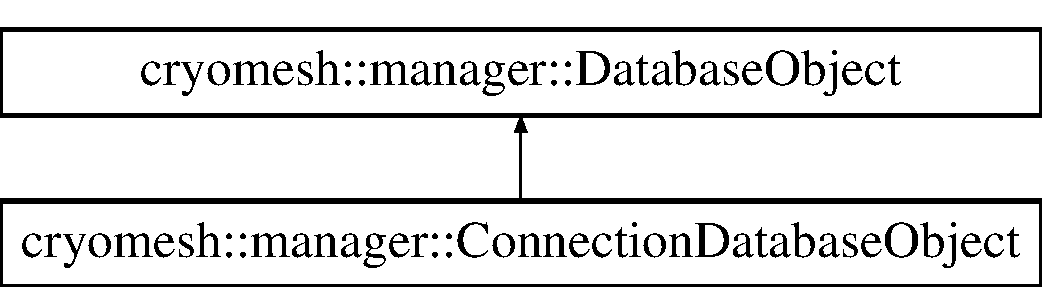
\includegraphics[height=2.000000cm]{classcryomesh_1_1manager_1_1ConnectionDatabaseObject}
\end{center}
\end{figure}
\subsection*{\-Public \-Member \-Functions}
\begin{DoxyCompactItemize}
\item 
\hyperlink{classcryomesh_1_1manager_1_1ConnectionDatabaseObject_a62f33a7c826d115aa981d3cca149e14b}{\-Connection\-Database\-Object} (const std\-::string \&uuid\-\_\-str, const std\-::string \&innode\-\_\-uuid\-\_\-str, const std\-::string \&outnode\-\_\-uuid\-\_\-str, const \hyperlink{classcryomesh_1_1common_1_1Cycle}{common\-::\-Cycle} \&\hyperlink{classcryomesh_1_1manager_1_1ConnectionDatabaseObject_a481ed7a285f11016e6f6182293cca49f}{cycle}, const int impulse\-\_\-count)
\begin{DoxyCompactList}\small\item\em \-Create database object from connection information. \end{DoxyCompactList}\item 
\hyperlink{classcryomesh_1_1manager_1_1ConnectionDatabaseObject_a8e38ce2ee538fc20ce2c2f04b6abce79}{\-Connection\-Database\-Object} (const std\-::string \&connection\-\_\-table\-\_\-entry)
\begin{DoxyCompactList}\small\item\em \-Create database object from a string database entry for a connection. \end{DoxyCompactList}\item 
virtual \hyperlink{classcryomesh_1_1manager_1_1ConnectionDatabaseObject_a1c34c6c64fcfc7c2aebc714b7b37d059}{$\sim$\-Connection\-Database\-Object} ()
\begin{DoxyCompactList}\small\item\em \-Default \-Destructor. \end{DoxyCompactList}\item 
virtual std\-::string \hyperlink{classcryomesh_1_1manager_1_1ConnectionDatabaseObject_ac7b22d25a4366175fd7d1578f476b125}{get\-Insert} (const std\-::string \&table) const 
\begin{DoxyCompactList}\small\item\em \-Get the string that can be used to insert the sql data. \end{DoxyCompactList}\item 
const std\-::string \& \hyperlink{classcryomesh_1_1manager_1_1ConnectionDatabaseObject_aa310082cf95a704640a068db4a328803}{get\-U\-U\-I\-D} () const 
\begin{DoxyCompactList}\small\item\em \-Get uuid variable of this object. \end{DoxyCompactList}\item 
const std\-::string \& \hyperlink{classcryomesh_1_1manager_1_1ConnectionDatabaseObject_a2e8384fe932c699e146511a628f16cff}{get\-Input\-Node\-U\-U\-I\-D} () const 
\begin{DoxyCompactList}\small\item\em \-Get input\-Node\-U\-U\-I\-D variable of this object. \end{DoxyCompactList}\item 
const std\-::string \& \hyperlink{classcryomesh_1_1manager_1_1ConnectionDatabaseObject_ab3488138917a89a2524c32d7999174c0}{get\-Output\-Node\-U\-U\-I\-D} () const 
\begin{DoxyCompactList}\small\item\em \-Get output\-Node\-U\-U\-I\-D variable of this object. \end{DoxyCompactList}\item 
const \hyperlink{classcryomesh_1_1common_1_1Cycle}{common\-::\-Cycle} \& \hyperlink{classcryomesh_1_1manager_1_1ConnectionDatabaseObject_acc8aa75ed2afb098ffba8cd79ed32b6b}{get\-Cycle} () const 
\begin{DoxyCompactList}\small\item\em \-Get cycle variable of this object. \end{DoxyCompactList}\item 
const int \& \hyperlink{classcryomesh_1_1manager_1_1ConnectionDatabaseObject_a6fe71c5af6d5e8c58546768c11f662f0}{get\-Impulse\-Count} () const 
\begin{DoxyCompactList}\small\item\em \-Get impulse\-Count variable of this object. \end{DoxyCompactList}\item 
std\-::string \hyperlink{classcryomesh_1_1manager_1_1DatabaseObject_a66ded4e1a1bccd65c94922648c7135c5}{get\-Key} (const std\-::string \&key) const 
\begin{DoxyCompactList}\small\item\em \-Return the string object associated with a key. \end{DoxyCompactList}\end{DoxyCompactItemize}
\subsection*{\-Static \-Public \-Member \-Functions}
\begin{DoxyCompactItemize}
\item 
static std\-::string \hyperlink{classcryomesh_1_1manager_1_1DatabaseObject_aa4ef26ce91fea092f146e67add491e0f}{find\-Value} (const std\-::string \&entry, const std\-::map$<$ std\-::string, std\-::string $>$ \&map)
\begin{DoxyCompactList}\small\item\em \-Find entries value in map or return null. \end{DoxyCompactList}\item 
static std\-::map$<$ std\-::string, \*
std\-::string $>$ \hyperlink{classcryomesh_1_1manager_1_1DatabaseObject_a04ce7c34b51e3290c972121cf2f16565}{get\-Column\-Map\-From\-Entry} (const std\-::string \&entry)
\begin{DoxyCompactList}\small\item\em \-Parse a string database entry, extract columns and values and return a map. \end{DoxyCompactList}\item 
{\footnotesize template$<$class T $>$ }\\static std\-::string \hyperlink{classcryomesh_1_1manager_1_1DatabaseObject_a1b37d9d07009ae1c71f644761d36b468}{to\-String} (\-T obj)
\begin{DoxyCompactList}\small\item\em \-Convert an templated object that can be piped to a stream to a string. \end{DoxyCompactList}\end{DoxyCompactItemize}
\subsection*{\-Static \-Public \-Attributes}
\begin{DoxyCompactItemize}
\item 
static const std\-::string \hyperlink{classcryomesh_1_1manager_1_1ConnectionDatabaseObject_ad04bc9639dd0ceed8d559f63cdc0c025}{\-I\-D\-\_\-\-T\-A\-G} = \char`\"{}id\char`\"{}
\item 
static const std\-::string \hyperlink{classcryomesh_1_1manager_1_1ConnectionDatabaseObject_a00720d641e03f298f88c5431d948fa1a}{\-I\-N\-P\-U\-T\-\_\-\-I\-D\-\_\-\-T\-A\-G} = \char`\"{}inputid\char`\"{}
\item 
static const std\-::string \hyperlink{classcryomesh_1_1manager_1_1ConnectionDatabaseObject_ac0ee0b21e1f626b12b125987283f7ebb}{\-O\-U\-T\-P\-U\-T\-\_\-\-I\-D\-\_\-\-T\-A\-G} = \char`\"{}outputid\char`\"{}
\item 
static const std\-::string \hyperlink{classcryomesh_1_1manager_1_1ConnectionDatabaseObject_a5e1505fdea7990278b9055b87d1071ef}{\-I\-M\-P\-U\-L\-S\-E\-\_\-\-C\-O\-U\-N\-T\-\_\-\-T\-A\-G} = \char`\"{}impulses\char`\"{}
\item 
static const std\-::string \hyperlink{classcryomesh_1_1manager_1_1ConnectionDatabaseObject_a6af5ded40e1ecffc6dbe072b68a7a153}{\-C\-Y\-C\-L\-E\-\_\-\-T\-A\-G} = \char`\"{}cycle\char`\"{}
\end{DoxyCompactItemize}
\subsection*{\-Protected \-Attributes}
\begin{DoxyCompactItemize}
\item 
std\-::map$<$ std\-::string, \*
std\-::string $>$ \hyperlink{classcryomesh_1_1manager_1_1DatabaseObject_a9c648bf09b9fd8b4d599b0d4f4abf531}{columns}
\end{DoxyCompactItemize}
\subsection*{\-Private \-Attributes}
\begin{DoxyCompactItemize}
\item 
std\-::string \hyperlink{classcryomesh_1_1manager_1_1ConnectionDatabaseObject_a31eb0b099470e77da0a89c5cef9d6f68}{uuid}
\item 
std\-::string \hyperlink{classcryomesh_1_1manager_1_1ConnectionDatabaseObject_a06774523f087375aaf58b69006b2943d}{input\-Node\-U\-U\-I\-D}
\item 
std\-::string \hyperlink{classcryomesh_1_1manager_1_1ConnectionDatabaseObject_a0b7a3185c6ef946c0afe806a364d13d5}{output\-Node\-U\-U\-I\-D}
\item 
\hyperlink{classcryomesh_1_1common_1_1Cycle}{common\-::\-Cycle} \hyperlink{classcryomesh_1_1manager_1_1ConnectionDatabaseObject_a481ed7a285f11016e6f6182293cca49f}{cycle}
\item 
int \hyperlink{classcryomesh_1_1manager_1_1ConnectionDatabaseObject_ae78ea47f996ccda8b67325edc74922c3}{impulse\-Count}
\end{DoxyCompactItemize}


\subsection{\-Detailed \-Description}


\-Definition at line 21 of file \-Connection\-Database\-Object.\-h.



\subsection{\-Constructor \& \-Destructor \-Documentation}
\hypertarget{classcryomesh_1_1manager_1_1ConnectionDatabaseObject_a62f33a7c826d115aa981d3cca149e14b}{\index{cryomesh\-::manager\-::\-Connection\-Database\-Object@{cryomesh\-::manager\-::\-Connection\-Database\-Object}!\-Connection\-Database\-Object@{\-Connection\-Database\-Object}}
\index{\-Connection\-Database\-Object@{\-Connection\-Database\-Object}!cryomesh::manager::ConnectionDatabaseObject@{cryomesh\-::manager\-::\-Connection\-Database\-Object}}
\subsubsection[{\-Connection\-Database\-Object}]{\setlength{\rightskip}{0pt plus 5cm}{\bf cryomesh\-::manager\-::\-Connection\-Database\-Object\-::\-Connection\-Database\-Object} (
\begin{DoxyParamCaption}
\item[{const std\-::string \&}]{uuid\-\_\-str, }
\item[{const std\-::string \&}]{innode\-\_\-uuid\-\_\-str, }
\item[{const std\-::string \&}]{outnode\-\_\-uuid\-\_\-str, }
\item[{const {\bf common\-::\-Cycle} \&}]{cycle, }
\item[{const int}]{impulse\-\_\-count}
\end{DoxyParamCaption}
)}}\label{classcryomesh_1_1manager_1_1ConnectionDatabaseObject_a62f33a7c826d115aa981d3cca149e14b}


\-Create database object from connection information. 


\begin{DoxyParams}{\-Parameters}
{\em std\-::string} & \-The uuid of the connection \\
\hline
{\em std\-::string} & \-The uuid of the input node \\
\hline
{\em std\-::string} & \-The uuid of the output node \\
\hline
{\em \hyperlink{classcryomesh_1_1common_1_1Cycle}{common\-::\-Cycle}} & \-The cycle of the entry \\
\hline
{\em int} & \-The impulse count of the connection on this entry \\
\hline
\end{DoxyParams}


\-Definition at line 20 of file \-Connection\-Database\-Object.\-cpp.



\-References cryomesh\-::manager\-::\-Database\-Object\-::columns, cycle, \-C\-Y\-C\-L\-E\-\_\-\-T\-A\-G, \-I\-D\-\_\-\-T\-A\-G, \-I\-M\-P\-U\-L\-S\-E\-\_\-\-C\-O\-U\-N\-T\-\_\-\-T\-A\-G, \-I\-N\-P\-U\-T\-\_\-\-I\-D\-\_\-\-T\-A\-G, \-O\-U\-T\-P\-U\-T\-\_\-\-I\-D\-\_\-\-T\-A\-G, and cryomesh\-::common\-::\-Cycle\-::to\-L\-Int().

\hypertarget{classcryomesh_1_1manager_1_1ConnectionDatabaseObject_a8e38ce2ee538fc20ce2c2f04b6abce79}{\index{cryomesh\-::manager\-::\-Connection\-Database\-Object@{cryomesh\-::manager\-::\-Connection\-Database\-Object}!\-Connection\-Database\-Object@{\-Connection\-Database\-Object}}
\index{\-Connection\-Database\-Object@{\-Connection\-Database\-Object}!cryomesh::manager::ConnectionDatabaseObject@{cryomesh\-::manager\-::\-Connection\-Database\-Object}}
\subsubsection[{\-Connection\-Database\-Object}]{\setlength{\rightskip}{0pt plus 5cm}{\bf cryomesh\-::manager\-::\-Connection\-Database\-Object\-::\-Connection\-Database\-Object} (
\begin{DoxyParamCaption}
\item[{const std\-::string \&}]{connection\-\_\-table\-\_\-entry}
\end{DoxyParamCaption}
)}}\label{classcryomesh_1_1manager_1_1ConnectionDatabaseObject_a8e38ce2ee538fc20ce2c2f04b6abce79}


\-Create database object from a string database entry for a connection. 


\begin{DoxyParams}{\-Parameters}
{\em std\-::string} & \-The database entry of the connection \\
\hline
\end{DoxyParams}


\-Definition at line 31 of file \-Connection\-Database\-Object.\-cpp.



\-References cycle, cryomesh\-::manager\-::\-Database\-Object\-::find\-Value(), cryomesh\-::manager\-::\-Database\-Object\-::get\-Column\-Map\-From\-Entry(), impulse\-Count, input\-Node\-U\-U\-I\-D, output\-Node\-U\-U\-I\-D, and uuid.

\hypertarget{classcryomesh_1_1manager_1_1ConnectionDatabaseObject_a1c34c6c64fcfc7c2aebc714b7b37d059}{\index{cryomesh\-::manager\-::\-Connection\-Database\-Object@{cryomesh\-::manager\-::\-Connection\-Database\-Object}!$\sim$\-Connection\-Database\-Object@{$\sim$\-Connection\-Database\-Object}}
\index{$\sim$\-Connection\-Database\-Object@{$\sim$\-Connection\-Database\-Object}!cryomesh::manager::ConnectionDatabaseObject@{cryomesh\-::manager\-::\-Connection\-Database\-Object}}
\subsubsection[{$\sim$\-Connection\-Database\-Object}]{\setlength{\rightskip}{0pt plus 5cm}{\bf cryomesh\-::manager\-::\-Connection\-Database\-Object\-::$\sim$\-Connection\-Database\-Object} (
\begin{DoxyParamCaption}
{}
\end{DoxyParamCaption}
)\hspace{0.3cm}{\ttfamily  \mbox{[}virtual\mbox{]}}}}\label{classcryomesh_1_1manager_1_1ConnectionDatabaseObject_a1c34c6c64fcfc7c2aebc714b7b37d059}


\-Default \-Destructor. 



\-Definition at line 66 of file \-Connection\-Database\-Object.\-cpp.



\subsection{\-Member \-Function \-Documentation}
\hypertarget{classcryomesh_1_1manager_1_1DatabaseObject_aa4ef26ce91fea092f146e67add491e0f}{\index{cryomesh\-::manager\-::\-Connection\-Database\-Object@{cryomesh\-::manager\-::\-Connection\-Database\-Object}!find\-Value@{find\-Value}}
\index{find\-Value@{find\-Value}!cryomesh::manager::ConnectionDatabaseObject@{cryomesh\-::manager\-::\-Connection\-Database\-Object}}
\subsubsection[{find\-Value}]{\setlength{\rightskip}{0pt plus 5cm}static std\-::string {\bf cryomesh\-::manager\-::\-Database\-Object\-::find\-Value} (
\begin{DoxyParamCaption}
\item[{const std\-::string \&}]{entry, }
\item[{const std\-::map$<$ std\-::string, std\-::string $>$ \&}]{map}
\end{DoxyParamCaption}
)\hspace{0.3cm}{\ttfamily  \mbox{[}inline, static, inherited\mbox{]}}}}\label{classcryomesh_1_1manager_1_1DatabaseObject_aa4ef26ce91fea092f146e67add491e0f}


\-Find entries value in map or return null. 


\begin{DoxyParams}{\-Parameters}
{\em std\-::string} & \-Entry to find \\
\hline
{\em std\-::map$<$std\-::string,std\-::string} & map to search\\
\hline
\end{DoxyParams}
\begin{DoxyReturn}{\-Returns}
\-Value of entry 
\end{DoxyReturn}


\-Definition at line 59 of file \-Database\-Object.\-h.



\-Referenced by \-Connection\-Database\-Object(), cryomesh\-::manager\-::\-Node\-Database\-Object\-::\-Node\-Database\-Object(), and cryomesh\-::manager\-::\-Pattern\-Database\-Object\-::\-Pattern\-Database\-Object().

\hypertarget{classcryomesh_1_1manager_1_1DatabaseObject_a04ce7c34b51e3290c972121cf2f16565}{\index{cryomesh\-::manager\-::\-Connection\-Database\-Object@{cryomesh\-::manager\-::\-Connection\-Database\-Object}!get\-Column\-Map\-From\-Entry@{get\-Column\-Map\-From\-Entry}}
\index{get\-Column\-Map\-From\-Entry@{get\-Column\-Map\-From\-Entry}!cryomesh::manager::ConnectionDatabaseObject@{cryomesh\-::manager\-::\-Connection\-Database\-Object}}
\subsubsection[{get\-Column\-Map\-From\-Entry}]{\setlength{\rightskip}{0pt plus 5cm}static std\-::map$<$std\-::string, std\-::string$>$ {\bf cryomesh\-::manager\-::\-Database\-Object\-::get\-Column\-Map\-From\-Entry} (
\begin{DoxyParamCaption}
\item[{const std\-::string \&}]{entry}
\end{DoxyParamCaption}
)\hspace{0.3cm}{\ttfamily  \mbox{[}inline, static, inherited\mbox{]}}}}\label{classcryomesh_1_1manager_1_1DatabaseObject_a04ce7c34b51e3290c972121cf2f16565}


\-Parse a string database entry, extract columns and values and return a map. 



\-Definition at line 72 of file \-Database\-Object.\-h.



\-Referenced by \-Connection\-Database\-Object(), cryomesh\-::manager\-::\-Node\-Database\-Object\-::\-Node\-Database\-Object(), and cryomesh\-::manager\-::\-Pattern\-Database\-Object\-::\-Pattern\-Database\-Object().

\hypertarget{classcryomesh_1_1manager_1_1ConnectionDatabaseObject_acc8aa75ed2afb098ffba8cd79ed32b6b}{\index{cryomesh\-::manager\-::\-Connection\-Database\-Object@{cryomesh\-::manager\-::\-Connection\-Database\-Object}!get\-Cycle@{get\-Cycle}}
\index{get\-Cycle@{get\-Cycle}!cryomesh::manager::ConnectionDatabaseObject@{cryomesh\-::manager\-::\-Connection\-Database\-Object}}
\subsubsection[{get\-Cycle}]{\setlength{\rightskip}{0pt plus 5cm}const {\bf common\-::\-Cycle} \& {\bf cryomesh\-::manager\-::\-Connection\-Database\-Object\-::get\-Cycle} (
\begin{DoxyParamCaption}
{}
\end{DoxyParamCaption}
) const}}\label{classcryomesh_1_1manager_1_1ConnectionDatabaseObject_acc8aa75ed2afb098ffba8cd79ed32b6b}


\-Get cycle variable of this object. 

\begin{DoxyReturn}{\-Returns}
std\-::string \-The cycle variable 
\end{DoxyReturn}


\-Definition at line 92 of file \-Connection\-Database\-Object.\-cpp.



\-References cycle.

\hypertarget{classcryomesh_1_1manager_1_1ConnectionDatabaseObject_a6fe71c5af6d5e8c58546768c11f662f0}{\index{cryomesh\-::manager\-::\-Connection\-Database\-Object@{cryomesh\-::manager\-::\-Connection\-Database\-Object}!get\-Impulse\-Count@{get\-Impulse\-Count}}
\index{get\-Impulse\-Count@{get\-Impulse\-Count}!cryomesh::manager::ConnectionDatabaseObject@{cryomesh\-::manager\-::\-Connection\-Database\-Object}}
\subsubsection[{get\-Impulse\-Count}]{\setlength{\rightskip}{0pt plus 5cm}const int \& {\bf cryomesh\-::manager\-::\-Connection\-Database\-Object\-::get\-Impulse\-Count} (
\begin{DoxyParamCaption}
{}
\end{DoxyParamCaption}
) const}}\label{classcryomesh_1_1manager_1_1ConnectionDatabaseObject_a6fe71c5af6d5e8c58546768c11f662f0}


\-Get impulse\-Count variable of this object. 

\begin{DoxyReturn}{\-Returns}
std\-::string \-The impulse\-Count variable 
\end{DoxyReturn}


\-Definition at line 96 of file \-Connection\-Database\-Object.\-cpp.



\-References impulse\-Count.

\hypertarget{classcryomesh_1_1manager_1_1ConnectionDatabaseObject_a2e8384fe932c699e146511a628f16cff}{\index{cryomesh\-::manager\-::\-Connection\-Database\-Object@{cryomesh\-::manager\-::\-Connection\-Database\-Object}!get\-Input\-Node\-U\-U\-I\-D@{get\-Input\-Node\-U\-U\-I\-D}}
\index{get\-Input\-Node\-U\-U\-I\-D@{get\-Input\-Node\-U\-U\-I\-D}!cryomesh::manager::ConnectionDatabaseObject@{cryomesh\-::manager\-::\-Connection\-Database\-Object}}
\subsubsection[{get\-Input\-Node\-U\-U\-I\-D}]{\setlength{\rightskip}{0pt plus 5cm}const std\-::string \& {\bf cryomesh\-::manager\-::\-Connection\-Database\-Object\-::get\-Input\-Node\-U\-U\-I\-D} (
\begin{DoxyParamCaption}
{}
\end{DoxyParamCaption}
) const}}\label{classcryomesh_1_1manager_1_1ConnectionDatabaseObject_a2e8384fe932c699e146511a628f16cff}


\-Get input\-Node\-U\-U\-I\-D variable of this object. 

\begin{DoxyReturn}{\-Returns}
std\-::string \-The input\-Node\-U\-U\-I\-D variable 
\end{DoxyReturn}


\-Definition at line 84 of file \-Connection\-Database\-Object.\-cpp.



\-References input\-Node\-U\-U\-I\-D.

\hypertarget{classcryomesh_1_1manager_1_1ConnectionDatabaseObject_ac7b22d25a4366175fd7d1578f476b125}{\index{cryomesh\-::manager\-::\-Connection\-Database\-Object@{cryomesh\-::manager\-::\-Connection\-Database\-Object}!get\-Insert@{get\-Insert}}
\index{get\-Insert@{get\-Insert}!cryomesh::manager::ConnectionDatabaseObject@{cryomesh\-::manager\-::\-Connection\-Database\-Object}}
\subsubsection[{get\-Insert}]{\setlength{\rightskip}{0pt plus 5cm}std\-::string {\bf cryomesh\-::manager\-::\-Connection\-Database\-Object\-::get\-Insert} (
\begin{DoxyParamCaption}
\item[{const std\-::string \&}]{table}
\end{DoxyParamCaption}
) const\hspace{0.3cm}{\ttfamily  \mbox{[}virtual\mbox{]}}}}\label{classcryomesh_1_1manager_1_1ConnectionDatabaseObject_ac7b22d25a4366175fd7d1578f476b125}


\-Get the string that can be used to insert the sql data. 

\begin{DoxyReturn}{\-Returns}
the sql command string to insert into this table 
\end{DoxyReturn}


\-Implements \hyperlink{classcryomesh_1_1manager_1_1DatabaseObject_ad55c6e711341a652790b97f549b0dc63}{cryomesh\-::manager\-::\-Database\-Object}.



\-Definition at line 69 of file \-Connection\-Database\-Object.\-cpp.



\-References \-C\-Y\-C\-L\-E\-\_\-\-T\-A\-G, cryomesh\-::manager\-::\-Database\-Object\-::get\-Key(), \-I\-D\-\_\-\-T\-A\-G, \-I\-M\-P\-U\-L\-S\-E\-\_\-\-C\-O\-U\-N\-T\-\_\-\-T\-A\-G, \-I\-N\-P\-U\-T\-\_\-\-I\-D\-\_\-\-T\-A\-G, and \-O\-U\-T\-P\-U\-T\-\_\-\-I\-D\-\_\-\-T\-A\-G.

\hypertarget{classcryomesh_1_1manager_1_1DatabaseObject_a66ded4e1a1bccd65c94922648c7135c5}{\index{cryomesh\-::manager\-::\-Connection\-Database\-Object@{cryomesh\-::manager\-::\-Connection\-Database\-Object}!get\-Key@{get\-Key}}
\index{get\-Key@{get\-Key}!cryomesh::manager::ConnectionDatabaseObject@{cryomesh\-::manager\-::\-Connection\-Database\-Object}}
\subsubsection[{get\-Key}]{\setlength{\rightskip}{0pt plus 5cm}std\-::string {\bf cryomesh\-::manager\-::\-Database\-Object\-::get\-Key} (
\begin{DoxyParamCaption}
\item[{const std\-::string \&}]{key}
\end{DoxyParamCaption}
) const\hspace{0.3cm}{\ttfamily  \mbox{[}inline, inherited\mbox{]}}}}\label{classcryomesh_1_1manager_1_1DatabaseObject_a66ded4e1a1bccd65c94922648c7135c5}


\-Return the string object associated with a key. 

\-::string \-The key to search for

\begin{DoxyReturn}{\-Returns}
std\-::string \-The object associated with the search key, \char`\"{}\char`\"{} if not found 
\end{DoxyReturn}


\-Definition at line 37 of file \-Database\-Object.\-h.



\-References cryomesh\-::manager\-::\-Database\-Object\-::columns.



\-Referenced by cryomesh\-::manager\-::\-Pattern\-Database\-Object\-::get\-Insert(), cryomesh\-::manager\-::\-Node\-Database\-Object\-::get\-Insert(), and get\-Insert().

\hypertarget{classcryomesh_1_1manager_1_1ConnectionDatabaseObject_ab3488138917a89a2524c32d7999174c0}{\index{cryomesh\-::manager\-::\-Connection\-Database\-Object@{cryomesh\-::manager\-::\-Connection\-Database\-Object}!get\-Output\-Node\-U\-U\-I\-D@{get\-Output\-Node\-U\-U\-I\-D}}
\index{get\-Output\-Node\-U\-U\-I\-D@{get\-Output\-Node\-U\-U\-I\-D}!cryomesh::manager::ConnectionDatabaseObject@{cryomesh\-::manager\-::\-Connection\-Database\-Object}}
\subsubsection[{get\-Output\-Node\-U\-U\-I\-D}]{\setlength{\rightskip}{0pt plus 5cm}const std\-::string \& {\bf cryomesh\-::manager\-::\-Connection\-Database\-Object\-::get\-Output\-Node\-U\-U\-I\-D} (
\begin{DoxyParamCaption}
{}
\end{DoxyParamCaption}
) const}}\label{classcryomesh_1_1manager_1_1ConnectionDatabaseObject_ab3488138917a89a2524c32d7999174c0}


\-Get output\-Node\-U\-U\-I\-D variable of this object. 

\begin{DoxyReturn}{\-Returns}
std\-::string \-The output\-Node\-U\-U\-I\-D variable 
\end{DoxyReturn}


\-Definition at line 88 of file \-Connection\-Database\-Object.\-cpp.



\-References output\-Node\-U\-U\-I\-D.

\hypertarget{classcryomesh_1_1manager_1_1ConnectionDatabaseObject_aa310082cf95a704640a068db4a328803}{\index{cryomesh\-::manager\-::\-Connection\-Database\-Object@{cryomesh\-::manager\-::\-Connection\-Database\-Object}!get\-U\-U\-I\-D@{get\-U\-U\-I\-D}}
\index{get\-U\-U\-I\-D@{get\-U\-U\-I\-D}!cryomesh::manager::ConnectionDatabaseObject@{cryomesh\-::manager\-::\-Connection\-Database\-Object}}
\subsubsection[{get\-U\-U\-I\-D}]{\setlength{\rightskip}{0pt plus 5cm}const std\-::string \& {\bf cryomesh\-::manager\-::\-Connection\-Database\-Object\-::get\-U\-U\-I\-D} (
\begin{DoxyParamCaption}
{}
\end{DoxyParamCaption}
) const}}\label{classcryomesh_1_1manager_1_1ConnectionDatabaseObject_aa310082cf95a704640a068db4a328803}


\-Get uuid variable of this object. 

\begin{DoxyReturn}{\-Returns}
std\-::string \-The uuid variable 
\end{DoxyReturn}


\-Definition at line 80 of file \-Connection\-Database\-Object.\-cpp.



\-References uuid.

\hypertarget{classcryomesh_1_1manager_1_1DatabaseObject_a1b37d9d07009ae1c71f644761d36b468}{\index{cryomesh\-::manager\-::\-Connection\-Database\-Object@{cryomesh\-::manager\-::\-Connection\-Database\-Object}!to\-String@{to\-String}}
\index{to\-String@{to\-String}!cryomesh::manager::ConnectionDatabaseObject@{cryomesh\-::manager\-::\-Connection\-Database\-Object}}
\subsubsection[{to\-String}]{\setlength{\rightskip}{0pt plus 5cm}template$<$class T $>$ static std\-::string {\bf cryomesh\-::manager\-::\-Database\-Object\-::to\-String} (
\begin{DoxyParamCaption}
\item[{\-T}]{obj}
\end{DoxyParamCaption}
)\hspace{0.3cm}{\ttfamily  \mbox{[}inline, static, inherited\mbox{]}}}}\label{classcryomesh_1_1manager_1_1DatabaseObject_a1b37d9d07009ae1c71f644761d36b468}


\-Convert an templated object that can be piped to a stream to a string. 


\begin{DoxyParams}{\-Parameters}
{\em \-T} & \-The object to get a string for \\
\hline
\end{DoxyParams}


\-Definition at line 108 of file \-Database\-Object.\-h.



\subsection{\-Member \-Data \-Documentation}
\hypertarget{classcryomesh_1_1manager_1_1DatabaseObject_a9c648bf09b9fd8b4d599b0d4f4abf531}{\index{cryomesh\-::manager\-::\-Connection\-Database\-Object@{cryomesh\-::manager\-::\-Connection\-Database\-Object}!columns@{columns}}
\index{columns@{columns}!cryomesh::manager::ConnectionDatabaseObject@{cryomesh\-::manager\-::\-Connection\-Database\-Object}}
\subsubsection[{columns}]{\setlength{\rightskip}{0pt plus 5cm}std\-::map$<$std\-::string, std\-::string$>$ {\bf cryomesh\-::manager\-::\-Database\-Object\-::columns}\hspace{0.3cm}{\ttfamily  \mbox{[}protected, inherited\mbox{]}}}}\label{classcryomesh_1_1manager_1_1DatabaseObject_a9c648bf09b9fd8b4d599b0d4f4abf531}


\-Definition at line 119 of file \-Database\-Object.\-h.



\-Referenced by \-Connection\-Database\-Object(), cryomesh\-::manager\-::\-Database\-Object\-::get\-Key(), cryomesh\-::manager\-::\-Node\-Database\-Object\-::\-Node\-Database\-Object(), and cryomesh\-::manager\-::\-Pattern\-Database\-Object\-::\-Pattern\-Database\-Object().

\hypertarget{classcryomesh_1_1manager_1_1ConnectionDatabaseObject_a481ed7a285f11016e6f6182293cca49f}{\index{cryomesh\-::manager\-::\-Connection\-Database\-Object@{cryomesh\-::manager\-::\-Connection\-Database\-Object}!cycle@{cycle}}
\index{cycle@{cycle}!cryomesh::manager::ConnectionDatabaseObject@{cryomesh\-::manager\-::\-Connection\-Database\-Object}}
\subsubsection[{cycle}]{\setlength{\rightskip}{0pt plus 5cm}{\bf common\-::\-Cycle} {\bf cryomesh\-::manager\-::\-Connection\-Database\-Object\-::cycle}\hspace{0.3cm}{\ttfamily  \mbox{[}private\mbox{]}}}}\label{classcryomesh_1_1manager_1_1ConnectionDatabaseObject_a481ed7a285f11016e6f6182293cca49f}


\-Definition at line 162 of file \-Connection\-Database\-Object.\-h.



\-Referenced by \-Connection\-Database\-Object(), and get\-Cycle().

\hypertarget{classcryomesh_1_1manager_1_1ConnectionDatabaseObject_a6af5ded40e1ecffc6dbe072b68a7a153}{\index{cryomesh\-::manager\-::\-Connection\-Database\-Object@{cryomesh\-::manager\-::\-Connection\-Database\-Object}!\-C\-Y\-C\-L\-E\-\_\-\-T\-A\-G@{\-C\-Y\-C\-L\-E\-\_\-\-T\-A\-G}}
\index{\-C\-Y\-C\-L\-E\-\_\-\-T\-A\-G@{\-C\-Y\-C\-L\-E\-\_\-\-T\-A\-G}!cryomesh::manager::ConnectionDatabaseObject@{cryomesh\-::manager\-::\-Connection\-Database\-Object}}
\subsubsection[{\-C\-Y\-C\-L\-E\-\_\-\-T\-A\-G}]{\setlength{\rightskip}{0pt plus 5cm}const std\-::string {\bf cryomesh\-::manager\-::\-Connection\-Database\-Object\-::\-C\-Y\-C\-L\-E\-\_\-\-T\-A\-G} = \char`\"{}cycle\char`\"{}\hspace{0.3cm}{\ttfamily  \mbox{[}static\mbox{]}}}}\label{classcryomesh_1_1manager_1_1ConnectionDatabaseObject_a6af5ded40e1ecffc6dbe072b68a7a153}


\-Definition at line 133 of file \-Connection\-Database\-Object.\-h.



\-Referenced by \-Connection\-Database\-Object(), and get\-Insert().

\hypertarget{classcryomesh_1_1manager_1_1ConnectionDatabaseObject_ad04bc9639dd0ceed8d559f63cdc0c025}{\index{cryomesh\-::manager\-::\-Connection\-Database\-Object@{cryomesh\-::manager\-::\-Connection\-Database\-Object}!\-I\-D\-\_\-\-T\-A\-G@{\-I\-D\-\_\-\-T\-A\-G}}
\index{\-I\-D\-\_\-\-T\-A\-G@{\-I\-D\-\_\-\-T\-A\-G}!cryomesh::manager::ConnectionDatabaseObject@{cryomesh\-::manager\-::\-Connection\-Database\-Object}}
\subsubsection[{\-I\-D\-\_\-\-T\-A\-G}]{\setlength{\rightskip}{0pt plus 5cm}const std\-::string {\bf cryomesh\-::manager\-::\-Connection\-Database\-Object\-::\-I\-D\-\_\-\-T\-A\-G} = \char`\"{}id\char`\"{}\hspace{0.3cm}{\ttfamily  \mbox{[}static\mbox{]}}}}\label{classcryomesh_1_1manager_1_1ConnectionDatabaseObject_ad04bc9639dd0ceed8d559f63cdc0c025}


\-Definition at line 106 of file \-Connection\-Database\-Object.\-h.



\-Referenced by \-Connection\-Database\-Object(), and get\-Insert().

\hypertarget{classcryomesh_1_1manager_1_1ConnectionDatabaseObject_a5e1505fdea7990278b9055b87d1071ef}{\index{cryomesh\-::manager\-::\-Connection\-Database\-Object@{cryomesh\-::manager\-::\-Connection\-Database\-Object}!\-I\-M\-P\-U\-L\-S\-E\-\_\-\-C\-O\-U\-N\-T\-\_\-\-T\-A\-G@{\-I\-M\-P\-U\-L\-S\-E\-\_\-\-C\-O\-U\-N\-T\-\_\-\-T\-A\-G}}
\index{\-I\-M\-P\-U\-L\-S\-E\-\_\-\-C\-O\-U\-N\-T\-\_\-\-T\-A\-G@{\-I\-M\-P\-U\-L\-S\-E\-\_\-\-C\-O\-U\-N\-T\-\_\-\-T\-A\-G}!cryomesh::manager::ConnectionDatabaseObject@{cryomesh\-::manager\-::\-Connection\-Database\-Object}}
\subsubsection[{\-I\-M\-P\-U\-L\-S\-E\-\_\-\-C\-O\-U\-N\-T\-\_\-\-T\-A\-G}]{\setlength{\rightskip}{0pt plus 5cm}const std\-::string {\bf cryomesh\-::manager\-::\-Connection\-Database\-Object\-::\-I\-M\-P\-U\-L\-S\-E\-\_\-\-C\-O\-U\-N\-T\-\_\-\-T\-A\-G} = \char`\"{}impulses\char`\"{}\hspace{0.3cm}{\ttfamily  \mbox{[}static\mbox{]}}}}\label{classcryomesh_1_1manager_1_1ConnectionDatabaseObject_a5e1505fdea7990278b9055b87d1071ef}


\-Definition at line 127 of file \-Connection\-Database\-Object.\-h.



\-Referenced by \-Connection\-Database\-Object(), and get\-Insert().

\hypertarget{classcryomesh_1_1manager_1_1ConnectionDatabaseObject_ae78ea47f996ccda8b67325edc74922c3}{\index{cryomesh\-::manager\-::\-Connection\-Database\-Object@{cryomesh\-::manager\-::\-Connection\-Database\-Object}!impulse\-Count@{impulse\-Count}}
\index{impulse\-Count@{impulse\-Count}!cryomesh::manager::ConnectionDatabaseObject@{cryomesh\-::manager\-::\-Connection\-Database\-Object}}
\subsubsection[{impulse\-Count}]{\setlength{\rightskip}{0pt plus 5cm}int {\bf cryomesh\-::manager\-::\-Connection\-Database\-Object\-::impulse\-Count}\hspace{0.3cm}{\ttfamily  \mbox{[}private\mbox{]}}}}\label{classcryomesh_1_1manager_1_1ConnectionDatabaseObject_ae78ea47f996ccda8b67325edc74922c3}


\-Definition at line 169 of file \-Connection\-Database\-Object.\-h.



\-Referenced by \-Connection\-Database\-Object(), and get\-Impulse\-Count().

\hypertarget{classcryomesh_1_1manager_1_1ConnectionDatabaseObject_a00720d641e03f298f88c5431d948fa1a}{\index{cryomesh\-::manager\-::\-Connection\-Database\-Object@{cryomesh\-::manager\-::\-Connection\-Database\-Object}!\-I\-N\-P\-U\-T\-\_\-\-I\-D\-\_\-\-T\-A\-G@{\-I\-N\-P\-U\-T\-\_\-\-I\-D\-\_\-\-T\-A\-G}}
\index{\-I\-N\-P\-U\-T\-\_\-\-I\-D\-\_\-\-T\-A\-G@{\-I\-N\-P\-U\-T\-\_\-\-I\-D\-\_\-\-T\-A\-G}!cryomesh::manager::ConnectionDatabaseObject@{cryomesh\-::manager\-::\-Connection\-Database\-Object}}
\subsubsection[{\-I\-N\-P\-U\-T\-\_\-\-I\-D\-\_\-\-T\-A\-G}]{\setlength{\rightskip}{0pt plus 5cm}const std\-::string {\bf cryomesh\-::manager\-::\-Connection\-Database\-Object\-::\-I\-N\-P\-U\-T\-\_\-\-I\-D\-\_\-\-T\-A\-G} = \char`\"{}inputid\char`\"{}\hspace{0.3cm}{\ttfamily  \mbox{[}static\mbox{]}}}}\label{classcryomesh_1_1manager_1_1ConnectionDatabaseObject_a00720d641e03f298f88c5431d948fa1a}


\-Definition at line 113 of file \-Connection\-Database\-Object.\-h.



\-Referenced by \-Connection\-Database\-Object(), and get\-Insert().

\hypertarget{classcryomesh_1_1manager_1_1ConnectionDatabaseObject_a06774523f087375aaf58b69006b2943d}{\index{cryomesh\-::manager\-::\-Connection\-Database\-Object@{cryomesh\-::manager\-::\-Connection\-Database\-Object}!input\-Node\-U\-U\-I\-D@{input\-Node\-U\-U\-I\-D}}
\index{input\-Node\-U\-U\-I\-D@{input\-Node\-U\-U\-I\-D}!cryomesh::manager::ConnectionDatabaseObject@{cryomesh\-::manager\-::\-Connection\-Database\-Object}}
\subsubsection[{input\-Node\-U\-U\-I\-D}]{\setlength{\rightskip}{0pt plus 5cm}std\-::string {\bf cryomesh\-::manager\-::\-Connection\-Database\-Object\-::input\-Node\-U\-U\-I\-D}\hspace{0.3cm}{\ttfamily  \mbox{[}private\mbox{]}}}}\label{classcryomesh_1_1manager_1_1ConnectionDatabaseObject_a06774523f087375aaf58b69006b2943d}


\-Definition at line 148 of file \-Connection\-Database\-Object.\-h.



\-Referenced by \-Connection\-Database\-Object(), and get\-Input\-Node\-U\-U\-I\-D().

\hypertarget{classcryomesh_1_1manager_1_1ConnectionDatabaseObject_ac0ee0b21e1f626b12b125987283f7ebb}{\index{cryomesh\-::manager\-::\-Connection\-Database\-Object@{cryomesh\-::manager\-::\-Connection\-Database\-Object}!\-O\-U\-T\-P\-U\-T\-\_\-\-I\-D\-\_\-\-T\-A\-G@{\-O\-U\-T\-P\-U\-T\-\_\-\-I\-D\-\_\-\-T\-A\-G}}
\index{\-O\-U\-T\-P\-U\-T\-\_\-\-I\-D\-\_\-\-T\-A\-G@{\-O\-U\-T\-P\-U\-T\-\_\-\-I\-D\-\_\-\-T\-A\-G}!cryomesh::manager::ConnectionDatabaseObject@{cryomesh\-::manager\-::\-Connection\-Database\-Object}}
\subsubsection[{\-O\-U\-T\-P\-U\-T\-\_\-\-I\-D\-\_\-\-T\-A\-G}]{\setlength{\rightskip}{0pt plus 5cm}const std\-::string {\bf cryomesh\-::manager\-::\-Connection\-Database\-Object\-::\-O\-U\-T\-P\-U\-T\-\_\-\-I\-D\-\_\-\-T\-A\-G} = \char`\"{}outputid\char`\"{}\hspace{0.3cm}{\ttfamily  \mbox{[}static\mbox{]}}}}\label{classcryomesh_1_1manager_1_1ConnectionDatabaseObject_ac0ee0b21e1f626b12b125987283f7ebb}


\-Definition at line 120 of file \-Connection\-Database\-Object.\-h.



\-Referenced by \-Connection\-Database\-Object(), and get\-Insert().

\hypertarget{classcryomesh_1_1manager_1_1ConnectionDatabaseObject_a0b7a3185c6ef946c0afe806a364d13d5}{\index{cryomesh\-::manager\-::\-Connection\-Database\-Object@{cryomesh\-::manager\-::\-Connection\-Database\-Object}!output\-Node\-U\-U\-I\-D@{output\-Node\-U\-U\-I\-D}}
\index{output\-Node\-U\-U\-I\-D@{output\-Node\-U\-U\-I\-D}!cryomesh::manager::ConnectionDatabaseObject@{cryomesh\-::manager\-::\-Connection\-Database\-Object}}
\subsubsection[{output\-Node\-U\-U\-I\-D}]{\setlength{\rightskip}{0pt plus 5cm}std\-::string {\bf cryomesh\-::manager\-::\-Connection\-Database\-Object\-::output\-Node\-U\-U\-I\-D}\hspace{0.3cm}{\ttfamily  \mbox{[}private\mbox{]}}}}\label{classcryomesh_1_1manager_1_1ConnectionDatabaseObject_a0b7a3185c6ef946c0afe806a364d13d5}


\-Definition at line 155 of file \-Connection\-Database\-Object.\-h.



\-Referenced by \-Connection\-Database\-Object(), and get\-Output\-Node\-U\-U\-I\-D().

\hypertarget{classcryomesh_1_1manager_1_1ConnectionDatabaseObject_a31eb0b099470e77da0a89c5cef9d6f68}{\index{cryomesh\-::manager\-::\-Connection\-Database\-Object@{cryomesh\-::manager\-::\-Connection\-Database\-Object}!uuid@{uuid}}
\index{uuid@{uuid}!cryomesh::manager::ConnectionDatabaseObject@{cryomesh\-::manager\-::\-Connection\-Database\-Object}}
\subsubsection[{uuid}]{\setlength{\rightskip}{0pt plus 5cm}std\-::string {\bf cryomesh\-::manager\-::\-Connection\-Database\-Object\-::uuid}\hspace{0.3cm}{\ttfamily  \mbox{[}private\mbox{]}}}}\label{classcryomesh_1_1manager_1_1ConnectionDatabaseObject_a31eb0b099470e77da0a89c5cef9d6f68}


\-Definition at line 141 of file \-Connection\-Database\-Object.\-h.



\-Referenced by \-Connection\-Database\-Object(), and get\-U\-U\-I\-D().



\-The documentation for this class was generated from the following files\-:\begin{DoxyCompactItemize}
\item 
/home/niall/\-Projects/\-Eclipse/\-C\-P\-P/cryomesh/src/manager/\hyperlink{ConnectionDatabaseObject_8h}{\-Connection\-Database\-Object.\-h}\item 
/home/niall/\-Projects/\-Eclipse/\-C\-P\-P/cryomesh/src/manager/\hyperlink{ConnectionDatabaseObject_8cpp}{\-Connection\-Database\-Object.\-cpp}\end{DoxyCompactItemize}

\hypertarget{classcryomesh_1_1components_1_1ConnectionMap}{\section{cryomesh\-:\-:components\-:\-:\-Connection\-Map \-Class \-Reference}
\label{classcryomesh_1_1components_1_1ConnectionMap}\index{cryomesh\-::components\-::\-Connection\-Map@{cryomesh\-::components\-::\-Connection\-Map}}
}


\-Helper class for \hyperlink{classcryomesh_1_1components_1_1ConnectionMap}{\-Connection\-Map} to \-Key\-Mapped\-Collection mapping.  




{\ttfamily \#include $<$\-Connection\-Map.\-h$>$}

\subsection*{\-Public \-Member \-Functions}
\begin{DoxyCompactItemize}
\item 
\hyperlink{classcryomesh_1_1components_1_1ConnectionMap_a512061797f1a737c674b6fae284295c7}{\-Connection\-Map} ()
\begin{DoxyCompactList}\small\item\em \-Default constructor. \end{DoxyCompactList}\item 
virtual \hyperlink{classcryomesh_1_1components_1_1ConnectionMap_a7c22a125652d332da2d8ceb194ad925e}{$\sim$\-Connection\-Map} ()
\begin{DoxyCompactList}\small\item\em \-Default destructor. \end{DoxyCompactList}\item 
virtual void \hyperlink{classcryomesh_1_1components_1_1ConnectionMap_aadb06c43b0eae37154fd7efb22a08949}{update} ()
\begin{DoxyCompactList}\small\item\em \-Update all entries in the map. \end{DoxyCompactList}\item 
boost\-::shared\-\_\-ptr\*
$<$ \hyperlink{classcryomesh_1_1state_1_1ActivityPattern}{state\-::\-Activity\-Pattern} $>$ \hyperlink{classcryomesh_1_1components_1_1ConnectionMap_a6de4ccc8a4a85199329c0d2a884a0dba}{get\-Activity\-Pattern} () const 
\begin{DoxyCompactList}\small\item\em \-Get activity pattern on current cycle. \end{DoxyCompactList}\item 
boost\-::shared\-\_\-ptr\*
$<$ \hyperlink{classcryomesh_1_1state_1_1ActivityPattern}{state\-::\-Activity\-Pattern} $>$ \hyperlink{classcryomesh_1_1components_1_1ConnectionMap_aeb905313475043da7bff0739925b5483}{get\-Activity\-Pattern} (const \hyperlink{classcryomesh_1_1common_1_1Cycle}{common\-::\-Cycle} \&cycle) const 
\begin{DoxyCompactList}\small\item\em \-Get activity pattern on cycle. \end{DoxyCompactList}\item 
const std\-::map\*
$<$ boost\-::uuids\-::uuid, \*
boost\-::shared\-\_\-ptr$<$ \hyperlink{classcryomesh_1_1components_1_1Connection}{\-Connection} $>$ $>$ \hyperlink{classcryomesh_1_1components_1_1ConnectionMap_afa08a6bd4894d7ff84db83a7eb15ad37}{get\-All\-Primary\-Input\-Connections} () const 
\item 
const std\-::map\*
$<$ boost\-::uuids\-::uuid, \*
boost\-::shared\-\_\-ptr$<$ \hyperlink{classcryomesh_1_1components_1_1Connection}{\-Connection} $>$ $>$ \hyperlink{classcryomesh_1_1components_1_1ConnectionMap_a9c6868c8f9b977ceb99e799fb6cc98eb}{get\-All\-Primary\-Output\-Connections} () const 
\end{DoxyCompactItemize}
\subsection*{\-Friends}
\begin{DoxyCompactItemize}
\item 
std\-::ostream \& \hyperlink{classcryomesh_1_1components_1_1ConnectionMap_a192eef17246516228fc7665ff541ee53}{operator$<$$<$} (std\-::ostream \&os, const \hyperlink{classcryomesh_1_1components_1_1ConnectionMap}{\-Connection\-Map} \&obj)
\begin{DoxyCompactList}\small\item\em \-To stream operator. \end{DoxyCompactList}\end{DoxyCompactItemize}


\subsection{\-Detailed \-Description}
\-Helper class for \hyperlink{classcryomesh_1_1components_1_1ConnectionMap}{\-Connection\-Map} to \-Key\-Mapped\-Collection mapping. 

\-Definition at line 26 of file \-Connection\-Map.\-h.



\subsection{\-Constructor \& \-Destructor \-Documentation}
\hypertarget{classcryomesh_1_1components_1_1ConnectionMap_a512061797f1a737c674b6fae284295c7}{\index{cryomesh\-::components\-::\-Connection\-Map@{cryomesh\-::components\-::\-Connection\-Map}!\-Connection\-Map@{\-Connection\-Map}}
\index{\-Connection\-Map@{\-Connection\-Map}!cryomesh::components::ConnectionMap@{cryomesh\-::components\-::\-Connection\-Map}}
\subsubsection[{\-Connection\-Map}]{\setlength{\rightskip}{0pt plus 5cm}{\bf cryomesh\-::components\-::\-Connection\-Map\-::\-Connection\-Map} (
\begin{DoxyParamCaption}
{}
\end{DoxyParamCaption}
)\hspace{0.3cm}{\ttfamily  \mbox{[}inline\mbox{]}}}}\label{classcryomesh_1_1components_1_1ConnectionMap_a512061797f1a737c674b6fae284295c7}


\-Default constructor. 



\-Definition at line 31 of file \-Connection\-Map.\-h.

\hypertarget{classcryomesh_1_1components_1_1ConnectionMap_a7c22a125652d332da2d8ceb194ad925e}{\index{cryomesh\-::components\-::\-Connection\-Map@{cryomesh\-::components\-::\-Connection\-Map}!$\sim$\-Connection\-Map@{$\sim$\-Connection\-Map}}
\index{$\sim$\-Connection\-Map@{$\sim$\-Connection\-Map}!cryomesh::components::ConnectionMap@{cryomesh\-::components\-::\-Connection\-Map}}
\subsubsection[{$\sim$\-Connection\-Map}]{\setlength{\rightskip}{0pt plus 5cm}virtual {\bf cryomesh\-::components\-::\-Connection\-Map\-::$\sim$\-Connection\-Map} (
\begin{DoxyParamCaption}
{}
\end{DoxyParamCaption}
)\hspace{0.3cm}{\ttfamily  \mbox{[}inline, virtual\mbox{]}}}}\label{classcryomesh_1_1components_1_1ConnectionMap_a7c22a125652d332da2d8ceb194ad925e}


\-Default destructor. 



\-Definition at line 37 of file \-Connection\-Map.\-h.



\subsection{\-Member \-Function \-Documentation}
\hypertarget{classcryomesh_1_1components_1_1ConnectionMap_a6de4ccc8a4a85199329c0d2a884a0dba}{\index{cryomesh\-::components\-::\-Connection\-Map@{cryomesh\-::components\-::\-Connection\-Map}!get\-Activity\-Pattern@{get\-Activity\-Pattern}}
\index{get\-Activity\-Pattern@{get\-Activity\-Pattern}!cryomesh::components::ConnectionMap@{cryomesh\-::components\-::\-Connection\-Map}}
\subsubsection[{get\-Activity\-Pattern}]{\setlength{\rightskip}{0pt plus 5cm}boost\-::shared\-\_\-ptr$<${\bf state\-::\-Activity\-Pattern}$>$ {\bf cryomesh\-::components\-::\-Connection\-Map\-::get\-Activity\-Pattern} (
\begin{DoxyParamCaption}
{}
\end{DoxyParamCaption}
) const\hspace{0.3cm}{\ttfamily  \mbox{[}inline\mbox{]}}}}\label{classcryomesh_1_1components_1_1ConnectionMap_a6de4ccc8a4a85199329c0d2a884a0dba}


\-Get activity pattern on current cycle. 

@ param const \-Cycle \& cycle \-Cycle to get activity on 

\-Definition at line 65 of file \-Connection\-Map.\-h.



\-References cryomesh\-::common\-::\-Time\-Keeper\-::get\-Time\-Keeper().

\hypertarget{classcryomesh_1_1components_1_1ConnectionMap_aeb905313475043da7bff0739925b5483}{\index{cryomesh\-::components\-::\-Connection\-Map@{cryomesh\-::components\-::\-Connection\-Map}!get\-Activity\-Pattern@{get\-Activity\-Pattern}}
\index{get\-Activity\-Pattern@{get\-Activity\-Pattern}!cryomesh::components::ConnectionMap@{cryomesh\-::components\-::\-Connection\-Map}}
\subsubsection[{get\-Activity\-Pattern}]{\setlength{\rightskip}{0pt plus 5cm}boost\-::shared\-\_\-ptr$<${\bf state\-::\-Activity\-Pattern}$>$ {\bf cryomesh\-::components\-::\-Connection\-Map\-::get\-Activity\-Pattern} (
\begin{DoxyParamCaption}
\item[{const {\bf common\-::\-Cycle} \&}]{cycle}
\end{DoxyParamCaption}
) const\hspace{0.3cm}{\ttfamily  \mbox{[}inline\mbox{]}}}}\label{classcryomesh_1_1components_1_1ConnectionMap_aeb905313475043da7bff0739925b5483}


\-Get activity pattern on cycle. 

@ param const \-Cycle \& cycle \-Cycle to get activity on 

\-Definition at line 75 of file \-Connection\-Map.\-h.

\hypertarget{classcryomesh_1_1components_1_1ConnectionMap_afa08a6bd4894d7ff84db83a7eb15ad37}{\index{cryomesh\-::components\-::\-Connection\-Map@{cryomesh\-::components\-::\-Connection\-Map}!get\-All\-Primary\-Input\-Connections@{get\-All\-Primary\-Input\-Connections}}
\index{get\-All\-Primary\-Input\-Connections@{get\-All\-Primary\-Input\-Connections}!cryomesh::components::ConnectionMap@{cryomesh\-::components\-::\-Connection\-Map}}
\subsubsection[{get\-All\-Primary\-Input\-Connections}]{\setlength{\rightskip}{0pt plus 5cm}const std\-::map$<$boost\-::uuids\-::uuid, boost\-::shared\-\_\-ptr$<${\bf \-Connection}$>$ $>$ {\bf cryomesh\-::components\-::\-Connection\-Map\-::get\-All\-Primary\-Input\-Connections} (
\begin{DoxyParamCaption}
{}
\end{DoxyParamCaption}
) const\hspace{0.3cm}{\ttfamily  \mbox{[}inline\mbox{]}}}}\label{classcryomesh_1_1components_1_1ConnectionMap_afa08a6bd4894d7ff84db83a7eb15ad37}


\-Definition at line 97 of file \-Connection\-Map.\-h.



\-Referenced by cryomesh\-::manipulators\-::\-Cluster\-Architect\-::get\-Random\-Connections().

\hypertarget{classcryomesh_1_1components_1_1ConnectionMap_a9c6868c8f9b977ceb99e799fb6cc98eb}{\index{cryomesh\-::components\-::\-Connection\-Map@{cryomesh\-::components\-::\-Connection\-Map}!get\-All\-Primary\-Output\-Connections@{get\-All\-Primary\-Output\-Connections}}
\index{get\-All\-Primary\-Output\-Connections@{get\-All\-Primary\-Output\-Connections}!cryomesh::components::ConnectionMap@{cryomesh\-::components\-::\-Connection\-Map}}
\subsubsection[{get\-All\-Primary\-Output\-Connections}]{\setlength{\rightskip}{0pt plus 5cm}const std\-::map$<$boost\-::uuids\-::uuid, boost\-::shared\-\_\-ptr$<${\bf \-Connection}$>$ $>$ {\bf cryomesh\-::components\-::\-Connection\-Map\-::get\-All\-Primary\-Output\-Connections} (
\begin{DoxyParamCaption}
{}
\end{DoxyParamCaption}
) const\hspace{0.3cm}{\ttfamily  \mbox{[}inline\mbox{]}}}}\label{classcryomesh_1_1components_1_1ConnectionMap_a9c6868c8f9b977ceb99e799fb6cc98eb}


\-Definition at line 119 of file \-Connection\-Map.\-h.



\-Referenced by cryomesh\-::manipulators\-::\-Cluster\-Architect\-::get\-Random\-Connections().

\hypertarget{classcryomesh_1_1components_1_1ConnectionMap_aadb06c43b0eae37154fd7efb22a08949}{\index{cryomesh\-::components\-::\-Connection\-Map@{cryomesh\-::components\-::\-Connection\-Map}!update@{update}}
\index{update@{update}!cryomesh::components::ConnectionMap@{cryomesh\-::components\-::\-Connection\-Map}}
\subsubsection[{update}]{\setlength{\rightskip}{0pt plus 5cm}virtual void {\bf cryomesh\-::components\-::\-Connection\-Map\-::update} (
\begin{DoxyParamCaption}
{}
\end{DoxyParamCaption}
)\hspace{0.3cm}{\ttfamily  \mbox{[}inline, virtual\mbox{]}}}}\label{classcryomesh_1_1components_1_1ConnectionMap_aadb06c43b0eae37154fd7efb22a08949}


\-Update all entries in the map. 



\-Definition at line 43 of file \-Connection\-Map.\-h.



\-Referenced by cryomesh\-::structures\-::\-Cluster\-::update(), and cryomesh\-::structures\-::\-Fibre\-::update().



\subsection{\-Friends \-And \-Related \-Function \-Documentation}
\hypertarget{classcryomesh_1_1components_1_1ConnectionMap_a192eef17246516228fc7665ff541ee53}{\index{cryomesh\-::components\-::\-Connection\-Map@{cryomesh\-::components\-::\-Connection\-Map}!operator$<$$<$@{operator$<$$<$}}
\index{operator$<$$<$@{operator$<$$<$}!cryomesh::components::ConnectionMap@{cryomesh\-::components\-::\-Connection\-Map}}
\subsubsection[{operator$<$$<$}]{\setlength{\rightskip}{0pt plus 5cm}std\-::ostream\& operator$<$$<$ (
\begin{DoxyParamCaption}
\item[{std\-::ostream \&}]{os, }
\item[{const {\bf \-Connection\-Map} \&}]{obj}
\end{DoxyParamCaption}
)\hspace{0.3cm}{\ttfamily  \mbox{[}friend\mbox{]}}}}\label{classcryomesh_1_1components_1_1ConnectionMap_a192eef17246516228fc7665ff541ee53}


\-To stream operator. 


\begin{DoxyParams}{\-Parameters}
{\em std\-::ostream} & \& os \-The output stream \\
\hline
{\em const} & \hyperlink{classcryomesh_1_1components_1_1ConnectionMap}{\-Connection\-Map} \& obj \-The object to stream\\
\hline
\end{DoxyParams}
\begin{DoxyReturn}{\-Returns}
std\-::ostream \& \-The output stream 
\end{DoxyReturn}


\-Definition at line 152 of file \-Connection\-Map.\-h.



\-The documentation for this class was generated from the following file\-:\begin{DoxyCompactItemize}
\item 
/home/niall/\-Projects/\-Eclipse/\-C\-P\-P/cryomesh/src/components/\hyperlink{ConnectionMap_8h}{\-Connection\-Map.\-h}\end{DoxyCompactItemize}

\hypertarget{structcryomesh_1_1manager_1_1ConnectionTableFormat}{\section{cryomesh\-:\-:manager\-:\-:\-Connection\-Table\-Format \-Struct \-Reference}
\label{structcryomesh_1_1manager_1_1ConnectionTableFormat}\index{cryomesh\-::manager\-::\-Connection\-Table\-Format@{cryomesh\-::manager\-::\-Connection\-Table\-Format}}
}


\-Struct representing a connections table structure.  




{\ttfamily \#include $<$\-Table\-Formats.\-h$>$}

\-Inheritance diagram for cryomesh\-:\-:manager\-:\-:\-Connection\-Table\-Format\-:\begin{figure}[H]
\begin{center}
\leavevmode
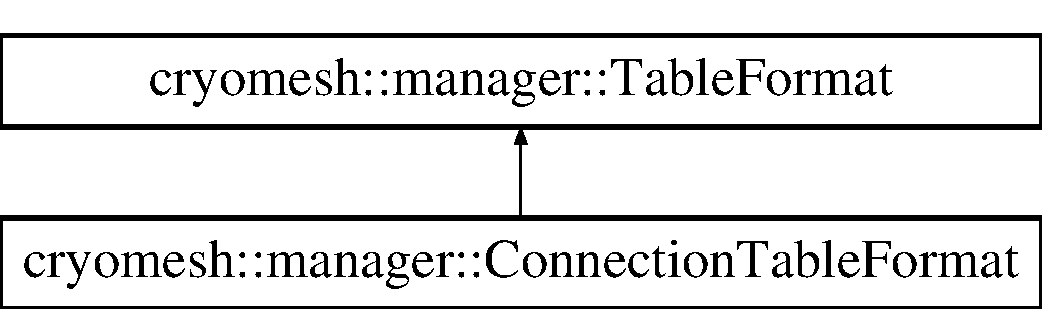
\includegraphics[height=2.000000cm]{structcryomesh_1_1manager_1_1ConnectionTableFormat}
\end{center}
\end{figure}
\subsection*{\-Public \-Member \-Functions}
\begin{DoxyCompactItemize}
\item 
\hyperlink{structcryomesh_1_1manager_1_1ConnectionTableFormat_a3aa9a5ff9e56afbb489fcfbed4dda041}{\-Connection\-Table\-Format} ()
\begin{DoxyCompactList}\small\item\em \-Default constructor will construct all the names and columns assiciated with a connections table. \end{DoxyCompactList}\item 
std\-::string \hyperlink{structcryomesh_1_1manager_1_1TableFormat_a3e797d6130c6b0745a1fac799c25677a}{get\-Name} () const 
\begin{DoxyCompactList}\small\item\em \-Return the name of the table. \end{DoxyCompactList}\item 
std\-::string \hyperlink{structcryomesh_1_1manager_1_1TableFormat_a2256ce39471582b92bf7cbb6eec74d30}{get\-Key} (const std\-::string \&key)
\begin{DoxyCompactList}\small\item\em \-Return the string object associated with a key. \end{DoxyCompactList}\item 
std\-::string \hyperlink{structcryomesh_1_1manager_1_1TableFormat_a898ae0d0c5490ccdf71aec5156b10fcc}{get\-Create\-Table} () const 
\begin{DoxyCompactList}\small\item\em \-Get the string that can be used to create the sql table. \end{DoxyCompactList}\end{DoxyCompactItemize}
\subsection*{\-Protected \-Attributes}
\begin{DoxyCompactItemize}
\item 
std\-::string \hyperlink{structcryomesh_1_1manager_1_1TableFormat_ab49912897ccb7fd0f8d42f1cc21332e8}{name}
\item 
std\-::map$<$ std\-::string, \*
std\-::string $>$ \hyperlink{structcryomesh_1_1manager_1_1TableFormat_a29ab6f4cfc0c56da1fa461ea665a1b61}{columns}
\end{DoxyCompactItemize}


\subsection{\-Detailed \-Description}
\-Struct representing a connections table structure. 

\-Definition at line 118 of file \-Table\-Formats.\-h.



\subsection{\-Constructor \& \-Destructor \-Documentation}
\hypertarget{structcryomesh_1_1manager_1_1ConnectionTableFormat_a3aa9a5ff9e56afbb489fcfbed4dda041}{\index{cryomesh\-::manager\-::\-Connection\-Table\-Format@{cryomesh\-::manager\-::\-Connection\-Table\-Format}!\-Connection\-Table\-Format@{\-Connection\-Table\-Format}}
\index{\-Connection\-Table\-Format@{\-Connection\-Table\-Format}!cryomesh::manager::ConnectionTableFormat@{cryomesh\-::manager\-::\-Connection\-Table\-Format}}
\subsubsection[{\-Connection\-Table\-Format}]{\setlength{\rightskip}{0pt plus 5cm}{\bf cryomesh\-::manager\-::\-Connection\-Table\-Format\-::\-Connection\-Table\-Format} (
\begin{DoxyParamCaption}
{}
\end{DoxyParamCaption}
)\hspace{0.3cm}{\ttfamily  \mbox{[}inline\mbox{]}}}}\label{structcryomesh_1_1manager_1_1ConnectionTableFormat_a3aa9a5ff9e56afbb489fcfbed4dda041}


\-Default constructor will construct all the names and columns assiciated with a connections table. 



\-Definition at line 123 of file \-Table\-Formats.\-h.



\-References cryomesh\-::manager\-::\-Table\-Format\-::columns, and cryomesh\-::manager\-::\-Table\-Format\-::name.



\subsection{\-Member \-Function \-Documentation}
\hypertarget{structcryomesh_1_1manager_1_1TableFormat_a898ae0d0c5490ccdf71aec5156b10fcc}{\index{cryomesh\-::manager\-::\-Connection\-Table\-Format@{cryomesh\-::manager\-::\-Connection\-Table\-Format}!get\-Create\-Table@{get\-Create\-Table}}
\index{get\-Create\-Table@{get\-Create\-Table}!cryomesh::manager::ConnectionTableFormat@{cryomesh\-::manager\-::\-Connection\-Table\-Format}}
\subsubsection[{get\-Create\-Table}]{\setlength{\rightskip}{0pt plus 5cm}std\-::string {\bf cryomesh\-::manager\-::\-Table\-Format\-::get\-Create\-Table} (
\begin{DoxyParamCaption}
{}
\end{DoxyParamCaption}
) const\hspace{0.3cm}{\ttfamily  \mbox{[}inline, inherited\mbox{]}}}}\label{structcryomesh_1_1manager_1_1TableFormat_a898ae0d0c5490ccdf71aec5156b10fcc}


\-Get the string that can be used to create the sql table. 

\begin{DoxyReturn}{\-Returns}
the sql command string to create this table 
\end{DoxyReturn}


\-Definition at line 60 of file \-Table\-Formats.\-h.



\-References cryomesh\-::manager\-::\-Table\-Format\-::columns, and cryomesh\-::manager\-::\-Table\-Format\-::get\-Name().

\hypertarget{structcryomesh_1_1manager_1_1TableFormat_a2256ce39471582b92bf7cbb6eec74d30}{\index{cryomesh\-::manager\-::\-Connection\-Table\-Format@{cryomesh\-::manager\-::\-Connection\-Table\-Format}!get\-Key@{get\-Key}}
\index{get\-Key@{get\-Key}!cryomesh::manager::ConnectionTableFormat@{cryomesh\-::manager\-::\-Connection\-Table\-Format}}
\subsubsection[{get\-Key}]{\setlength{\rightskip}{0pt plus 5cm}std\-::string {\bf cryomesh\-::manager\-::\-Table\-Format\-::get\-Key} (
\begin{DoxyParamCaption}
\item[{const std\-::string \&}]{key}
\end{DoxyParamCaption}
)\hspace{0.3cm}{\ttfamily  \mbox{[}inline, inherited\mbox{]}}}}\label{structcryomesh_1_1manager_1_1TableFormat_a2256ce39471582b92bf7cbb6eec74d30}


\-Return the string object associated with a key. 

\-::string \-The key to search for

\begin{DoxyReturn}{\-Returns}
std\-::string \-The object associated with the search key, \char`\"{}\char`\"{} if not found 
\end{DoxyReturn}


\-Definition at line 45 of file \-Table\-Formats.\-h.



\-References cryomesh\-::manager\-::\-Table\-Format\-::columns.

\hypertarget{structcryomesh_1_1manager_1_1TableFormat_a3e797d6130c6b0745a1fac799c25677a}{\index{cryomesh\-::manager\-::\-Connection\-Table\-Format@{cryomesh\-::manager\-::\-Connection\-Table\-Format}!get\-Name@{get\-Name}}
\index{get\-Name@{get\-Name}!cryomesh::manager::ConnectionTableFormat@{cryomesh\-::manager\-::\-Connection\-Table\-Format}}
\subsubsection[{get\-Name}]{\setlength{\rightskip}{0pt plus 5cm}std\-::string {\bf cryomesh\-::manager\-::\-Table\-Format\-::get\-Name} (
\begin{DoxyParamCaption}
{}
\end{DoxyParamCaption}
) const\hspace{0.3cm}{\ttfamily  \mbox{[}inline, inherited\mbox{]}}}}\label{structcryomesh_1_1manager_1_1TableFormat_a3e797d6130c6b0745a1fac799c25677a}


\-Return the name of the table. 

\begin{DoxyReturn}{\-Returns}
std\-::string \-The name of the table 
\end{DoxyReturn}


\-Definition at line 32 of file \-Table\-Formats.\-h.



\-References cryomesh\-::manager\-::\-Table\-Format\-::name.



\-Referenced by cryomesh\-::manager\-::\-Table\-Format\-::get\-Create\-Table(), cryomesh\-::manager\-::\-Database\-Manager\-::insert\-Connection(), cryomesh\-::manager\-::\-Database\-Manager\-::insert\-Node(), and cryomesh\-::manager\-::\-Database\-Manager\-::insert\-Output\-Pattern().



\subsection{\-Member \-Data \-Documentation}
\hypertarget{structcryomesh_1_1manager_1_1TableFormat_a29ab6f4cfc0c56da1fa461ea665a1b61}{\index{cryomesh\-::manager\-::\-Connection\-Table\-Format@{cryomesh\-::manager\-::\-Connection\-Table\-Format}!columns@{columns}}
\index{columns@{columns}!cryomesh::manager::ConnectionTableFormat@{cryomesh\-::manager\-::\-Connection\-Table\-Format}}
\subsubsection[{columns}]{\setlength{\rightskip}{0pt plus 5cm}std\-::map$<$std\-::string, std\-::string$>$ {\bf cryomesh\-::manager\-::\-Table\-Format\-::columns}\hspace{0.3cm}{\ttfamily  \mbox{[}protected, inherited\mbox{]}}}}\label{structcryomesh_1_1manager_1_1TableFormat_a29ab6f4cfc0c56da1fa461ea665a1b61}


\-Definition at line 93 of file \-Table\-Formats.\-h.



\-Referenced by \-Connection\-Table\-Format(), cryomesh\-::manager\-::\-Table\-Format\-::get\-Create\-Table(), cryomesh\-::manager\-::\-Table\-Format\-::get\-Key(), cryomesh\-::manager\-::\-Input\-Patterns\-Table\-Format\-::\-Input\-Patterns\-Table\-Format(), cryomesh\-::manager\-::\-Node\-Table\-Format\-::\-Node\-Table\-Format(), and cryomesh\-::manager\-::\-Output\-Patterns\-Table\-Format\-::\-Output\-Patterns\-Table\-Format().

\hypertarget{structcryomesh_1_1manager_1_1TableFormat_ab49912897ccb7fd0f8d42f1cc21332e8}{\index{cryomesh\-::manager\-::\-Connection\-Table\-Format@{cryomesh\-::manager\-::\-Connection\-Table\-Format}!name@{name}}
\index{name@{name}!cryomesh::manager::ConnectionTableFormat@{cryomesh\-::manager\-::\-Connection\-Table\-Format}}
\subsubsection[{name}]{\setlength{\rightskip}{0pt plus 5cm}std\-::string {\bf cryomesh\-::manager\-::\-Table\-Format\-::name}\hspace{0.3cm}{\ttfamily  \mbox{[}protected, inherited\mbox{]}}}}\label{structcryomesh_1_1manager_1_1TableFormat_ab49912897ccb7fd0f8d42f1cc21332e8}


\-Definition at line 86 of file \-Table\-Formats.\-h.



\-Referenced by \-Connection\-Table\-Format(), cryomesh\-::manager\-::\-Table\-Format\-::get\-Name(), cryomesh\-::manager\-::\-Input\-Patterns\-Table\-Format\-::\-Input\-Patterns\-Table\-Format(), cryomesh\-::manager\-::\-Node\-Table\-Format\-::\-Node\-Table\-Format(), and cryomesh\-::manager\-::\-Output\-Patterns\-Table\-Format\-::\-Output\-Patterns\-Table\-Format().



\-The documentation for this struct was generated from the following file\-:\begin{DoxyCompactItemize}
\item 
/home/niall/\-Projects/\-Eclipse/\-C\-P\-P/cryomesh/src/manager/\hyperlink{TableFormats_8h}{\-Table\-Formats.\-h}\end{DoxyCompactItemize}

\hypertarget{classcryomesh_1_1common_1_1Connector}{\section{cryomesh\-:\-:common\-:\-:\-Connector$<$ \-U, \-T $>$ \-Class \-Template \-Reference}
\label{classcryomesh_1_1common_1_1Connector}\index{cryomesh\-::common\-::\-Connector$<$ U, T $>$@{cryomesh\-::common\-::\-Connector$<$ U, T $>$}}
}


\hyperlink{classcryomesh_1_1common_1_1Connector}{\-Connector} is a template to add connectable functionality between two classes.  




{\ttfamily \#include $<$\-Connector.\-h$>$}

\subsection*{\-Public \-Member \-Functions}
\begin{DoxyCompactItemize}
\item 
\hyperlink{classcryomesh_1_1common_1_1Connector_a44c721dbd4fbf74f4b71528e440cbbac}{\-Connector} (const unsigned int max\-\_\-inputs=0, const unsigned int max\-\_\-outputs=0)
\item 
virtual \hyperlink{classcryomesh_1_1common_1_1Connector_adf967a4426097b1f8152711ba9e8edb7}{$\sim$\-Connector} ()
\item 
bool \hyperlink{classcryomesh_1_1common_1_1Connector_aa8eab10d81bfa921ad1341ad1fbc9a4d}{connect\-Input} (const boost\-::shared\-\_\-ptr$<$ \-T $>$ obj)
\begin{DoxyCompactList}\small\item\em \-Connect a unit to this one as an input. \end{DoxyCompactList}\item 
bool \hyperlink{classcryomesh_1_1common_1_1Connector_a94c014ba589b22076c84fd8394b96c8d}{connect\-Inputs} (const std\-::vector$<$ boost\-::shared\-\_\-ptr$<$ \-T $>$ $>$ \&list)
\begin{DoxyCompactList}\small\item\em \-Connect a list of units to this one as inputs. \end{DoxyCompactList}\item 
bool \hyperlink{classcryomesh_1_1common_1_1Connector_ad3287ece677524300b761e57ecb109de}{connect\-Inputs} (const std\-::initializer\-\_\-list$<$ boost\-::shared\-\_\-ptr$<$ \-T $>$ $>$ \&list)
\begin{DoxyCompactList}\small\item\em \-Connect an initialiser list of units to this one as inputs. \end{DoxyCompactList}\item 
bool \hyperlink{classcryomesh_1_1common_1_1Connector_a1fa0ff922e03cbb5654a2de468af9d41}{connect\-Output} (const boost\-::shared\-\_\-ptr$<$ \-T $>$ \&obj)
\begin{DoxyCompactList}\small\item\em \-Connect a unit to this one as an output. \end{DoxyCompactList}\item 
bool \hyperlink{classcryomesh_1_1common_1_1Connector_a4c962f5b074b2d81e4952cfbb11ab974}{connect\-Outputs} (const std\-::vector$<$ boost\-::shared\-\_\-ptr$<$ \-T $>$ $>$ \&list)
\begin{DoxyCompactList}\small\item\em \-Connect a list of units to this one as outputs. \end{DoxyCompactList}\item 
bool \hyperlink{classcryomesh_1_1common_1_1Connector_a8fca74791240e711bdd6c89b26759390}{connect\-Outputs} (const std\-::initializer\-\_\-list$<$ boost\-::shared\-\_\-ptr$<$ \-T $>$ $>$ \&list)
\begin{DoxyCompactList}\small\item\em \-Connect an initialiser list of units to this one as outputs. \end{DoxyCompactList}\item 
bool \hyperlink{classcryomesh_1_1common_1_1Connector_a6726db121456485ea580ba7f9365bb37}{disconnect\-Input} (const boost\-::shared\-\_\-ptr$<$ \-T $>$ \&obj)
\begin{DoxyCompactList}\small\item\em \-Disconnect an input to this unit. \end{DoxyCompactList}\item 
bool \hyperlink{classcryomesh_1_1common_1_1Connector_a9de5eb37810b4d1563bff904b5bc545e}{disconnect\-Input} (const boost\-::uuids\-::uuid \&id)
\begin{DoxyCompactList}\small\item\em \-Disconnect an input to this unit. \end{DoxyCompactList}\item 
bool \hyperlink{classcryomesh_1_1common_1_1Connector_af37d582516d355642f6a14544f21e1b3}{disconnect\-Inputs} (const std\-::vector$<$ boost\-::shared\-\_\-ptr$<$ \-T $>$ $>$ \&list)
\begin{DoxyCompactList}\small\item\em \-Disconnect a list of input units from this one. \end{DoxyCompactList}\item 
bool \hyperlink{classcryomesh_1_1common_1_1Connector_aa6eb7d8ec6d50abeb7942ca4d3955927}{disconnect\-Inputs} (const std\-::initializer\-\_\-list$<$ boost\-::shared\-\_\-ptr$<$ \-T $>$ $>$ \&list)
\begin{DoxyCompactList}\small\item\em \-Disconnect an initialiser list of input units from this one. \end{DoxyCompactList}\item 
bool \hyperlink{classcryomesh_1_1common_1_1Connector_a8df62ec2ead7b69453c74398d8182a39}{disconnect\-Inputs} (const std\-::vector$<$ boost\-::uuids\-::uuid $>$ \&list)
\begin{DoxyCompactList}\small\item\em \-Disconnect a list of input units from this one. \end{DoxyCompactList}\item 
bool \hyperlink{classcryomesh_1_1common_1_1Connector_aebc08e7a92cec11c1353391f9145d841}{disconnect\-Inputs} (const std\-::initializer\-\_\-list$<$ boost\-::uuids\-::uuid $>$ \&list)
\begin{DoxyCompactList}\small\item\em \-Disconnect an initialiser list of input units from this one. \end{DoxyCompactList}\item 
bool \hyperlink{classcryomesh_1_1common_1_1Connector_ae158782ad5bf70ce2913be421ace2e4d}{disconnect\-All\-Inputs} ()
\begin{DoxyCompactList}\small\item\em \-Disconnect all input units from this one. \end{DoxyCompactList}\item 
bool \hyperlink{classcryomesh_1_1common_1_1Connector_ab0c0f68c11aa53c3b407f613ffa212f1}{disconnect\-Output} (const boost\-::shared\-\_\-ptr$<$ \-T $>$ \&obj)
\begin{DoxyCompactList}\small\item\em \-Disconnect an output to this unit. \end{DoxyCompactList}\item 
bool \hyperlink{classcryomesh_1_1common_1_1Connector_a12a36aef140f4a58c688d899d086f8d1}{disconnect\-Output} (const boost\-::uuids\-::uuid \&id)
\begin{DoxyCompactList}\small\item\em \-Disconnect an output to this unit. \end{DoxyCompactList}\item 
bool \hyperlink{classcryomesh_1_1common_1_1Connector_a680ddbd6bd137f05b5a8ab9e28b73f48}{disconnect\-Outputs} (const std\-::vector$<$ boost\-::shared\-\_\-ptr$<$ \-T $>$ $>$ \&list)
\begin{DoxyCompactList}\small\item\em \-Disconnect a list of \-Output units from this one. \end{DoxyCompactList}\item 
bool \hyperlink{classcryomesh_1_1common_1_1Connector_a5b3daf294a8f5e808b7cada38cbd1cfd}{disconnect\-Outputs} (const std\-::initializer\-\_\-list$<$ boost\-::shared\-\_\-ptr$<$ \-T $>$ $>$ \&list)
\begin{DoxyCompactList}\small\item\em \-Disconnect an initialiser list of \-Output units from this one. \end{DoxyCompactList}\item 
bool \hyperlink{classcryomesh_1_1common_1_1Connector_a5a6ab355b767129f60f4042a734e1db0}{disconnect\-Outputs} (const std\-::vector$<$ boost\-::uuids\-::uuid $>$ \&list)
\begin{DoxyCompactList}\small\item\em \-Disconnect a uuid list of \-Output units from this one. \end{DoxyCompactList}\item 
bool \hyperlink{classcryomesh_1_1common_1_1Connector_adb34713ed33984fef703a8a1ad342624}{disconnect\-Outputs} (const std\-::initializer\-\_\-list$<$ boost\-::uuids\-::uuid $>$ \&list)
\begin{DoxyCompactList}\small\item\em \-Disconnect an uuid initiaialiser list of \-Output units from this one. \end{DoxyCompactList}\item 
bool \hyperlink{classcryomesh_1_1common_1_1Connector_afff7a004da2146ab0fca902204bd62ee}{disconnect\-All\-Outputs} ()
\begin{DoxyCompactList}\small\item\em \-Disconnect all \-Output units from this one. \end{DoxyCompactList}\item 
const std\-::map\*
$<$ boost\-::uuids\-::uuid, \*
boost\-::shared\-\_\-ptr$<$ \-T $>$ $>$ \& \hyperlink{classcryomesh_1_1common_1_1Connector_af294647fe03f03108b2edd81c11aaa0a}{get\-Inputs} () const 
\begin{DoxyCompactList}\small\item\em \-Get all inputs. \end{DoxyCompactList}\item 
const std\-::list\*
$<$ boost\-::uuids\-::uuid $>$ \hyperlink{classcryomesh_1_1common_1_1Connector_acd6f00383ee6fd73ef8374494ce09865}{get\-Inputs\-U\-U\-I\-D} () const 
\item 
const std\-::list\*
$<$ boost\-::uuids\-::uuid $>$ \hyperlink{classcryomesh_1_1common_1_1Connector_acccc3d12685c44062af17cf5d7d78b6a}{get\-Outputs\-U\-U\-I\-D} () const 
\item 
std\-::map$<$ boost\-::uuids\-::uuid, \*
boost\-::shared\-\_\-ptr$<$ \-T $>$ $>$ \& \hyperlink{classcryomesh_1_1common_1_1Connector_a673488ae2b7b9c00658bf4e4b99b26f2}{get\-Mutable\-Inputs} ()
\begin{DoxyCompactList}\small\item\em \-Get all inputs as mutable object. \end{DoxyCompactList}\item 
const std\-::map\*
$<$ boost\-::uuids\-::uuid, \*
boost\-::shared\-\_\-ptr$<$ \-T $>$ $>$ \& \hyperlink{classcryomesh_1_1common_1_1Connector_af108b3bdc8adee1d2f6ce34c6b7781e6}{get\-Outputs} () const 
\begin{DoxyCompactList}\small\item\em \-Get all outputs. \end{DoxyCompactList}\item 
std\-::map$<$ boost\-::uuids\-::uuid, \*
boost\-::shared\-\_\-ptr$<$ \-T $>$ $>$ \& \hyperlink{classcryomesh_1_1common_1_1Connector_a974b1c610f3c949d64560f2d0d44f5eb}{get\-Mutable\-Outputs} ()
\begin{DoxyCompactList}\small\item\em \-Get all outputs as mutable object. \end{DoxyCompactList}\end{DoxyCompactItemize}
\subsection*{\-Protected \-Member \-Functions}
\begin{DoxyCompactItemize}
\item 
boost\-::shared\-\_\-ptr$<$ \-T $>$ \hyperlink{classcryomesh_1_1common_1_1Connector_a1adff096f822eee244c7c26cd7f3fc3f}{connect} (const boost\-::shared\-\_\-ptr$<$ \-T $>$ obj, std\-::map$<$ boost\-::uuids\-::uuid, boost\-::shared\-\_\-ptr$<$ \-T $>$ $>$ \&objs, unsigned int max\-\_\-connections)
\begin{DoxyCompactList}\small\item\em \-Connect up an object using the supplied map. \end{DoxyCompactList}\item 
boost\-::shared\-\_\-ptr$<$ \-T $>$ \hyperlink{classcryomesh_1_1common_1_1Connector_abdabb88b660f2f71a25a15f81fe5b683}{disconnect} (const boost\-::shared\-\_\-ptr$<$ \-T $>$ obj, std\-::map$<$ boost\-::uuids\-::uuid, boost\-::shared\-\_\-ptr$<$ \-T $>$ $>$ \&objs)
\begin{DoxyCompactList}\small\item\em \-Disconnect an object using the supplied map. \end{DoxyCompactList}\item 
boost\-::shared\-\_\-ptr$<$ \-T $>$ \hyperlink{classcryomesh_1_1common_1_1Connector_a3ddc25ebd1129d2d5d93126f768fd1ee}{disconnect} (const boost\-::uuids\-::uuid \&id, std\-::map$<$ boost\-::uuids\-::uuid, boost\-::shared\-\_\-ptr$<$ \-T $>$ $>$ \&objs)
\begin{DoxyCompactList}\small\item\em \-Disconnect an object using the supplied map. \end{DoxyCompactList}\end{DoxyCompactItemize}
\subsection*{\-Protected \-Attributes}
\begin{DoxyCompactItemize}
\item 
std\-::map$<$ boost\-::uuids\-::uuid, \*
boost\-::shared\-\_\-ptr$<$ \-T $>$ $>$ \hyperlink{classcryomesh_1_1common_1_1Connector_a4b53045b5f70f35b9cf8838474bdbc97}{minputs}
\item 
std\-::map$<$ boost\-::uuids\-::uuid, \*
boost\-::shared\-\_\-ptr$<$ \-T $>$ $>$ \hyperlink{classcryomesh_1_1common_1_1Connector_a3a7175d8c33a8f5cd72592748c6dc15f}{moutputs}
\item 
unsigned int \hyperlink{classcryomesh_1_1common_1_1Connector_aed34a9f056b3f718cbf5669717d46694}{max\-Inputs}
\item 
unsigned int \hyperlink{classcryomesh_1_1common_1_1Connector_aa30303b7f79bab1364ff8ba53ea3fb25}{max\-Outputs}
\end{DoxyCompactItemize}
\subsection*{\-Friends}
\begin{DoxyCompactItemize}
\item 
std\-::ostream \& \hyperlink{classcryomesh_1_1common_1_1Connector_a821dbf25de8022d484c33728df5a69f5}{operator$<$$<$} (std\-::ostream \&os, const \hyperlink{classcryomesh_1_1common_1_1Connector}{\-Connector}$<$ \-U, \-T $>$ \&obj)
\begin{DoxyCompactList}\small\item\em \-To stream operator. \end{DoxyCompactList}\end{DoxyCompactItemize}


\subsection{\-Detailed \-Description}
\subsubsection*{template$<$class \-U, class \-T$>$class cryomesh\-::common\-::\-Connector$<$ U, T $>$}

\hyperlink{classcryomesh_1_1common_1_1Connector}{\-Connector} is a template to add connectable functionality between two classes. 

\-Represents a template to add connectable funtionality between class \-U as the central connectable and class \-T as those objects it can be connected to 

\-Definition at line 33 of file \-Connector.\-h.



\subsection{\-Constructor \& \-Destructor \-Documentation}
\hypertarget{classcryomesh_1_1common_1_1Connector_a44c721dbd4fbf74f4b71528e440cbbac}{\index{cryomesh\-::common\-::\-Connector@{cryomesh\-::common\-::\-Connector}!\-Connector@{\-Connector}}
\index{\-Connector@{\-Connector}!cryomesh::common::Connector@{cryomesh\-::common\-::\-Connector}}
\subsubsection[{\-Connector}]{\setlength{\rightskip}{0pt plus 5cm}template$<$class \-U, class \-T$>$ {\bf cryomesh\-::common\-::\-Connector}$<$ \-U, \-T $>$\-::{\bf \-Connector} (
\begin{DoxyParamCaption}
\item[{const unsigned int}]{max\-\_\-inputs = {\ttfamily 0}, }
\item[{const unsigned int}]{max\-\_\-outputs = {\ttfamily 0}}
\end{DoxyParamCaption}
)\hspace{0.3cm}{\ttfamily  \mbox{[}inline\mbox{]}}}}\label{classcryomesh_1_1common_1_1Connector_a44c721dbd4fbf74f4b71528e440cbbac}


\-Definition at line 35 of file \-Connector.\-h.

\hypertarget{classcryomesh_1_1common_1_1Connector_adf967a4426097b1f8152711ba9e8edb7}{\index{cryomesh\-::common\-::\-Connector@{cryomesh\-::common\-::\-Connector}!$\sim$\-Connector@{$\sim$\-Connector}}
\index{$\sim$\-Connector@{$\sim$\-Connector}!cryomesh::common::Connector@{cryomesh\-::common\-::\-Connector}}
\subsubsection[{$\sim$\-Connector}]{\setlength{\rightskip}{0pt plus 5cm}template$<$class \-U, class \-T$>$ virtual {\bf cryomesh\-::common\-::\-Connector}$<$ \-U, \-T $>$\-::$\sim${\bf \-Connector} (
\begin{DoxyParamCaption}
{}
\end{DoxyParamCaption}
)\hspace{0.3cm}{\ttfamily  \mbox{[}inline, virtual\mbox{]}}}}\label{classcryomesh_1_1common_1_1Connector_adf967a4426097b1f8152711ba9e8edb7}


\-Definition at line 39 of file \-Connector.\-h.



\subsection{\-Member \-Function \-Documentation}
\hypertarget{classcryomesh_1_1common_1_1Connector_a1adff096f822eee244c7c26cd7f3fc3f}{\index{cryomesh\-::common\-::\-Connector@{cryomesh\-::common\-::\-Connector}!connect@{connect}}
\index{connect@{connect}!cryomesh::common::Connector@{cryomesh\-::common\-::\-Connector}}
\subsubsection[{connect}]{\setlength{\rightskip}{0pt plus 5cm}template$<$class \-U, class \-T$>$ boost\-::shared\-\_\-ptr$<$\-T$>$ {\bf cryomesh\-::common\-::\-Connector}$<$ \-U, \-T $>$\-::{\bf connect} (
\begin{DoxyParamCaption}
\item[{const boost\-::shared\-\_\-ptr$<$ \-T $>$}]{obj, }
\item[{std\-::map$<$ boost\-::uuids\-::uuid, boost\-::shared\-\_\-ptr$<$ \-T $>$ $>$ \&}]{objs, }
\item[{unsigned int}]{max\-\_\-connections}
\end{DoxyParamCaption}
)\hspace{0.3cm}{\ttfamily  \mbox{[}inline, protected\mbox{]}}}}\label{classcryomesh_1_1common_1_1Connector_a1adff096f822eee244c7c26cd7f3fc3f}


\-Connect up an object using the supplied map. 


\begin{DoxyParams}{\-Parameters}
{\em boost\-::shared\-\_\-ptr$<$\-T$>$} & obj \hyperlink{structcryomesh_1_1Pointer}{\-Pointer} to the object that is to be connected \\
\hline
{\em std\-::map$<$boost\-::uuids\-::uuid,boost\-::shared\-\_\-ptr$<$\-T$>$} & $>$ objs \-The map that will be used to connect the object \\
\hline
{\em unsinged} & int \-Maximum connections to allow\\
\hline
\end{DoxyParams}
\begin{DoxyReturn}{\-Returns}
\hyperlink{structcryomesh_1_1Pointer}{\-Pointer} to the connected object 
\end{DoxyReturn}


\-Definition at line 655 of file \-Connector.\-h.



\-Referenced by cryomesh\-::common\-::\-Connector$<$ Fibre, Cluster $>$\-::connect\-Input(), and cryomesh\-::common\-::\-Connector$<$ Fibre, Cluster $>$\-::connect\-Output().

\hypertarget{classcryomesh_1_1common_1_1Connector_aa8eab10d81bfa921ad1341ad1fbc9a4d}{\index{cryomesh\-::common\-::\-Connector@{cryomesh\-::common\-::\-Connector}!connect\-Input@{connect\-Input}}
\index{connect\-Input@{connect\-Input}!cryomesh::common::Connector@{cryomesh\-::common\-::\-Connector}}
\subsubsection[{connect\-Input}]{\setlength{\rightskip}{0pt plus 5cm}template$<$class \-U, class \-T$>$ bool {\bf cryomesh\-::common\-::\-Connector}$<$ \-U, \-T $>$\-::{\bf connect\-Input} (
\begin{DoxyParamCaption}
\item[{const boost\-::shared\-\_\-ptr$<$ \-T $>$}]{obj}
\end{DoxyParamCaption}
)\hspace{0.3cm}{\ttfamily  \mbox{[}inline\mbox{]}}}}\label{classcryomesh_1_1common_1_1Connector_aa8eab10d81bfa921ad1341ad1fbc9a4d}


\-Connect a unit to this one as an input. 


\begin{DoxyParams}{\-Parameters}
{\em boost\-::shared\-\_\-ptr$<$\-T$>$} & obj \hyperlink{structcryomesh_1_1Pointer}{\-Pointer} to the object to be connected as input\\
\hline
\end{DoxyParams}
\begin{DoxyReturn}{\-Returns}
true if connection succeeds, false otherwise 
\end{DoxyReturn}


\-Definition at line 53 of file \-Connector.\-h.



\-Referenced by cryomesh\-::structures\-::\-Fibre\-::connect\-All\-Connections(), and cryomesh\-::common\-::\-Connector$<$ Fibre, Cluster $>$\-::connect\-Inputs().

\hypertarget{classcryomesh_1_1common_1_1Connector_a94c014ba589b22076c84fd8394b96c8d}{\index{cryomesh\-::common\-::\-Connector@{cryomesh\-::common\-::\-Connector}!connect\-Inputs@{connect\-Inputs}}
\index{connect\-Inputs@{connect\-Inputs}!cryomesh::common::Connector@{cryomesh\-::common\-::\-Connector}}
\subsubsection[{connect\-Inputs}]{\setlength{\rightskip}{0pt plus 5cm}template$<$class \-U, class \-T$>$ bool {\bf cryomesh\-::common\-::\-Connector}$<$ \-U, \-T $>$\-::{\bf connect\-Inputs} (
\begin{DoxyParamCaption}
\item[{const std\-::vector$<$ boost\-::shared\-\_\-ptr$<$ \-T $>$ $>$ \&}]{list}
\end{DoxyParamCaption}
)\hspace{0.3cm}{\ttfamily  \mbox{[}inline\mbox{]}}}}\label{classcryomesh_1_1common_1_1Connector_a94c014ba589b22076c84fd8394b96c8d}


\-Connect a list of units to this one as inputs. 


\begin{DoxyParams}{\-Parameters}
{\em std\-::vector$<$boost\-::shared\-\_\-ptr$<$\-T$>$} & $>$ list \-List of pointers to objects to be connected as inputs\\
\hline
\end{DoxyParams}
\begin{DoxyReturn}{\-Returns}
true if all connections succeed, false otherwise 
\end{DoxyReturn}


\-Definition at line 73 of file \-Connector.\-h.

\hypertarget{classcryomesh_1_1common_1_1Connector_ad3287ece677524300b761e57ecb109de}{\index{cryomesh\-::common\-::\-Connector@{cryomesh\-::common\-::\-Connector}!connect\-Inputs@{connect\-Inputs}}
\index{connect\-Inputs@{connect\-Inputs}!cryomesh::common::Connector@{cryomesh\-::common\-::\-Connector}}
\subsubsection[{connect\-Inputs}]{\setlength{\rightskip}{0pt plus 5cm}template$<$class \-U, class \-T$>$ bool {\bf cryomesh\-::common\-::\-Connector}$<$ \-U, \-T $>$\-::{\bf connect\-Inputs} (
\begin{DoxyParamCaption}
\item[{const std\-::initializer\-\_\-list$<$ boost\-::shared\-\_\-ptr$<$ \-T $>$ $>$ \&}]{list}
\end{DoxyParamCaption}
)\hspace{0.3cm}{\ttfamily  \mbox{[}inline\mbox{]}}}}\label{classcryomesh_1_1common_1_1Connector_ad3287ece677524300b761e57ecb109de}


\-Connect an initialiser list of units to this one as inputs. 


\begin{DoxyParams}{\-Parameters}
{\em std\-::initializer\-\_\-list$<$boost\-::shared\-\_\-ptr$<$} & \-T $>$ $>$ list \-Initialiser list of pointers to objects to be connected as input\\
\hline
\end{DoxyParams}
\begin{DoxyReturn}{\-Returns}
true if all connections succeed, false otherwise 
\end{DoxyReturn}


\-Definition at line 97 of file \-Connector.\-h.

\hypertarget{classcryomesh_1_1common_1_1Connector_a1fa0ff922e03cbb5654a2de468af9d41}{\index{cryomesh\-::common\-::\-Connector@{cryomesh\-::common\-::\-Connector}!connect\-Output@{connect\-Output}}
\index{connect\-Output@{connect\-Output}!cryomesh::common::Connector@{cryomesh\-::common\-::\-Connector}}
\subsubsection[{connect\-Output}]{\setlength{\rightskip}{0pt plus 5cm}template$<$class \-U, class \-T$>$ bool {\bf cryomesh\-::common\-::\-Connector}$<$ \-U, \-T $>$\-::{\bf connect\-Output} (
\begin{DoxyParamCaption}
\item[{const boost\-::shared\-\_\-ptr$<$ \-T $>$ \&}]{obj}
\end{DoxyParamCaption}
)\hspace{0.3cm}{\ttfamily  \mbox{[}inline\mbox{]}}}}\label{classcryomesh_1_1common_1_1Connector_a1fa0ff922e03cbb5654a2de468af9d41}


\-Connect a unit to this one as an output. 


\begin{DoxyParams}{\-Parameters}
{\em boost\-::shared\-\_\-ptr$<$\-T$>$} & obj \hyperlink{structcryomesh_1_1Pointer}{\-Pointer} to the object to be connected as output\\
\hline
\end{DoxyParams}
\begin{DoxyReturn}{\-Returns}
true if connection succeeds, false otherwise 
\end{DoxyReturn}


\-Definition at line 122 of file \-Connector.\-h.



\-Referenced by cryomesh\-::structures\-::\-Fibre\-::connect\-All\-Connections(), and cryomesh\-::common\-::\-Connector$<$ Fibre, Cluster $>$\-::connect\-Outputs().

\hypertarget{classcryomesh_1_1common_1_1Connector_a4c962f5b074b2d81e4952cfbb11ab974}{\index{cryomesh\-::common\-::\-Connector@{cryomesh\-::common\-::\-Connector}!connect\-Outputs@{connect\-Outputs}}
\index{connect\-Outputs@{connect\-Outputs}!cryomesh::common::Connector@{cryomesh\-::common\-::\-Connector}}
\subsubsection[{connect\-Outputs}]{\setlength{\rightskip}{0pt plus 5cm}template$<$class \-U, class \-T$>$ bool {\bf cryomesh\-::common\-::\-Connector}$<$ \-U, \-T $>$\-::{\bf connect\-Outputs} (
\begin{DoxyParamCaption}
\item[{const std\-::vector$<$ boost\-::shared\-\_\-ptr$<$ \-T $>$ $>$ \&}]{list}
\end{DoxyParamCaption}
)\hspace{0.3cm}{\ttfamily  \mbox{[}inline\mbox{]}}}}\label{classcryomesh_1_1common_1_1Connector_a4c962f5b074b2d81e4952cfbb11ab974}


\-Connect a list of units to this one as outputs. 


\begin{DoxyParams}{\-Parameters}
{\em std\-::vector$<$boost\-::shared\-\_\-ptr$<$\-T$>$} & $>$ list \-List of pointers to objects to be connected as outputs\\
\hline
\end{DoxyParams}
\begin{DoxyReturn}{\-Returns}
true if all connections succeed, false otherwise 
\end{DoxyReturn}


\-Definition at line 142 of file \-Connector.\-h.

\hypertarget{classcryomesh_1_1common_1_1Connector_a8fca74791240e711bdd6c89b26759390}{\index{cryomesh\-::common\-::\-Connector@{cryomesh\-::common\-::\-Connector}!connect\-Outputs@{connect\-Outputs}}
\index{connect\-Outputs@{connect\-Outputs}!cryomesh::common::Connector@{cryomesh\-::common\-::\-Connector}}
\subsubsection[{connect\-Outputs}]{\setlength{\rightskip}{0pt plus 5cm}template$<$class \-U, class \-T$>$ bool {\bf cryomesh\-::common\-::\-Connector}$<$ \-U, \-T $>$\-::{\bf connect\-Outputs} (
\begin{DoxyParamCaption}
\item[{const std\-::initializer\-\_\-list$<$ boost\-::shared\-\_\-ptr$<$ \-T $>$ $>$ \&}]{list}
\end{DoxyParamCaption}
)\hspace{0.3cm}{\ttfamily  \mbox{[}inline\mbox{]}}}}\label{classcryomesh_1_1common_1_1Connector_a8fca74791240e711bdd6c89b26759390}


\-Connect an initialiser list of units to this one as outputs. 


\begin{DoxyParams}{\-Parameters}
{\em std\-::initializer\-\_\-list$<$boost\-::shared\-\_\-ptr$<$} & \-T $>$ $>$ list \-Initialiser list of pointers to objects to be connected as outputs\\
\hline
\end{DoxyParams}
\begin{DoxyReturn}{\-Returns}
true if all connections succeed, false otherwise 
\end{DoxyReturn}


\-Definition at line 167 of file \-Connector.\-h.

\hypertarget{classcryomesh_1_1common_1_1Connector_abdabb88b660f2f71a25a15f81fe5b683}{\index{cryomesh\-::common\-::\-Connector@{cryomesh\-::common\-::\-Connector}!disconnect@{disconnect}}
\index{disconnect@{disconnect}!cryomesh::common::Connector@{cryomesh\-::common\-::\-Connector}}
\subsubsection[{disconnect}]{\setlength{\rightskip}{0pt plus 5cm}template$<$class \-U, class \-T$>$ boost\-::shared\-\_\-ptr$<$\-T$>$ {\bf cryomesh\-::common\-::\-Connector}$<$ \-U, \-T $>$\-::{\bf disconnect} (
\begin{DoxyParamCaption}
\item[{const boost\-::shared\-\_\-ptr$<$ \-T $>$}]{obj, }
\item[{std\-::map$<$ boost\-::uuids\-::uuid, boost\-::shared\-\_\-ptr$<$ \-T $>$ $>$ \&}]{objs}
\end{DoxyParamCaption}
)\hspace{0.3cm}{\ttfamily  \mbox{[}inline, protected\mbox{]}}}}\label{classcryomesh_1_1common_1_1Connector_abdabb88b660f2f71a25a15f81fe5b683}


\-Disconnect an object using the supplied map. 


\begin{DoxyParams}{\-Parameters}
{\em boost\-::shared\-\_\-ptr$<$\-T$>$} & obj \hyperlink{structcryomesh_1_1Pointer}{\-Pointer} to the object that is to be disconnected \\
\hline
{\em std\-::map$<$boost\-::uuids\-::uuid,boost\-::shared\-\_\-ptr$<$\-T$>$} & $>$ objs \-The map that will be used to disconnect the object\\
\hline
\end{DoxyParams}
\begin{DoxyReturn}{\-Returns}
\hyperlink{structcryomesh_1_1Pointer}{\-Pointer} to the disconnected object, pointer is 0 is object was not found 
\end{DoxyReturn}


\-Definition at line 685 of file \-Connector.\-h.



\-Referenced by cryomesh\-::common\-::\-Connector$<$ Fibre, Cluster $>$\-::disconnect\-Input(), and cryomesh\-::common\-::\-Connector$<$ Fibre, Cluster $>$\-::disconnect\-Output().

\hypertarget{classcryomesh_1_1common_1_1Connector_a3ddc25ebd1129d2d5d93126f768fd1ee}{\index{cryomesh\-::common\-::\-Connector@{cryomesh\-::common\-::\-Connector}!disconnect@{disconnect}}
\index{disconnect@{disconnect}!cryomesh::common::Connector@{cryomesh\-::common\-::\-Connector}}
\subsubsection[{disconnect}]{\setlength{\rightskip}{0pt plus 5cm}template$<$class \-U, class \-T$>$ boost\-::shared\-\_\-ptr$<$\-T$>$ {\bf cryomesh\-::common\-::\-Connector}$<$ \-U, \-T $>$\-::{\bf disconnect} (
\begin{DoxyParamCaption}
\item[{const boost\-::uuids\-::uuid \&}]{id, }
\item[{std\-::map$<$ boost\-::uuids\-::uuid, boost\-::shared\-\_\-ptr$<$ \-T $>$ $>$ \&}]{objs}
\end{DoxyParamCaption}
)\hspace{0.3cm}{\ttfamily  \mbox{[}inline, protected\mbox{]}}}}\label{classcryomesh_1_1common_1_1Connector_a3ddc25ebd1129d2d5d93126f768fd1ee}


\-Disconnect an object using the supplied map. 


\begin{DoxyParams}{\-Parameters}
{\em boost\-::uuids\-::uuid} & id \-The uuid of the object that is to be disconnected \\
\hline
{\em std\-::map$<$boost\-::uuids\-::uuid,boost\-::shared\-\_\-ptr$<$\-T$>$} & $>$ \& objs \-The map that will be used to disconnect the object\\
\hline
\end{DoxyParams}
\begin{DoxyReturn}{\-Returns}
\hyperlink{structcryomesh_1_1Pointer}{\-Pointer} to the disconnected object, pointer is null is object was not found 
\end{DoxyReturn}


\-Definition at line 724 of file \-Connector.\-h.

\hypertarget{classcryomesh_1_1common_1_1Connector_ae158782ad5bf70ce2913be421ace2e4d}{\index{cryomesh\-::common\-::\-Connector@{cryomesh\-::common\-::\-Connector}!disconnect\-All\-Inputs@{disconnect\-All\-Inputs}}
\index{disconnect\-All\-Inputs@{disconnect\-All\-Inputs}!cryomesh::common::Connector@{cryomesh\-::common\-::\-Connector}}
\subsubsection[{disconnect\-All\-Inputs}]{\setlength{\rightskip}{0pt plus 5cm}template$<$class \-U, class \-T$>$ bool {\bf cryomesh\-::common\-::\-Connector}$<$ \-U, \-T $>$\-::{\bf disconnect\-All\-Inputs} (
\begin{DoxyParamCaption}
{}
\end{DoxyParamCaption}
)\hspace{0.3cm}{\ttfamily  \mbox{[}inline\mbox{]}}}}\label{classcryomesh_1_1common_1_1Connector_ae158782ad5bf70ce2913be421ace2e4d}


\-Disconnect all input units from this one. 

\begin{DoxyReturn}{\-Returns}
true if all disconnections succeed, false otherwise 
\end{DoxyReturn}


\-Definition at line 332 of file \-Connector.\-h.



\-Referenced by cryomesh\-::structures\-::\-Fibre\-::disconnect\-All\-Connections().

\hypertarget{classcryomesh_1_1common_1_1Connector_afff7a004da2146ab0fca902204bd62ee}{\index{cryomesh\-::common\-::\-Connector@{cryomesh\-::common\-::\-Connector}!disconnect\-All\-Outputs@{disconnect\-All\-Outputs}}
\index{disconnect\-All\-Outputs@{disconnect\-All\-Outputs}!cryomesh::common::Connector@{cryomesh\-::common\-::\-Connector}}
\subsubsection[{disconnect\-All\-Outputs}]{\setlength{\rightskip}{0pt plus 5cm}template$<$class \-U, class \-T$>$ bool {\bf cryomesh\-::common\-::\-Connector}$<$ \-U, \-T $>$\-::{\bf disconnect\-All\-Outputs} (
\begin{DoxyParamCaption}
{}
\end{DoxyParamCaption}
)\hspace{0.3cm}{\ttfamily  \mbox{[}inline\mbox{]}}}}\label{classcryomesh_1_1common_1_1Connector_afff7a004da2146ab0fca902204bd62ee}


\-Disconnect all \-Output units from this one. 

\begin{DoxyReturn}{\-Returns}
true if all disconnections succeed, false otherwise 
\end{DoxyReturn}


\-Definition at line 500 of file \-Connector.\-h.



\-Referenced by cryomesh\-::structures\-::\-Fibre\-::disconnect\-All\-Connections().

\hypertarget{classcryomesh_1_1common_1_1Connector_a6726db121456485ea580ba7f9365bb37}{\index{cryomesh\-::common\-::\-Connector@{cryomesh\-::common\-::\-Connector}!disconnect\-Input@{disconnect\-Input}}
\index{disconnect\-Input@{disconnect\-Input}!cryomesh::common::Connector@{cryomesh\-::common\-::\-Connector}}
\subsubsection[{disconnect\-Input}]{\setlength{\rightskip}{0pt plus 5cm}template$<$class \-U, class \-T$>$ bool {\bf cryomesh\-::common\-::\-Connector}$<$ \-U, \-T $>$\-::{\bf disconnect\-Input} (
\begin{DoxyParamCaption}
\item[{const boost\-::shared\-\_\-ptr$<$ \-T $>$ \&}]{obj}
\end{DoxyParamCaption}
)\hspace{0.3cm}{\ttfamily  \mbox{[}inline\mbox{]}}}}\label{classcryomesh_1_1common_1_1Connector_a6726db121456485ea580ba7f9365bb37}


\-Disconnect an input to this unit. 


\begin{DoxyParams}{\-Parameters}
{\em boost\-::shared\-\_\-ptr$<$\-T$>$} & obj \hyperlink{structcryomesh_1_1Pointer}{\-Pointer} to the object to be disconnected from input\\
\hline
\end{DoxyParams}
\begin{DoxyReturn}{\-Returns}
true if disconnection succeeds, false otherwise 
\end{DoxyReturn}


\-Definition at line 193 of file \-Connector.\-h.



\-Referenced by cryomesh\-::common\-::\-Connector$<$ Fibre, Cluster $>$\-::disconnect\-All\-Inputs(), and cryomesh\-::common\-::\-Connector$<$ Fibre, Cluster $>$\-::disconnect\-Inputs().

\hypertarget{classcryomesh_1_1common_1_1Connector_a9de5eb37810b4d1563bff904b5bc545e}{\index{cryomesh\-::common\-::\-Connector@{cryomesh\-::common\-::\-Connector}!disconnect\-Input@{disconnect\-Input}}
\index{disconnect\-Input@{disconnect\-Input}!cryomesh::common::Connector@{cryomesh\-::common\-::\-Connector}}
\subsubsection[{disconnect\-Input}]{\setlength{\rightskip}{0pt plus 5cm}template$<$class \-U, class \-T$>$ bool {\bf cryomesh\-::common\-::\-Connector}$<$ \-U, \-T $>$\-::{\bf disconnect\-Input} (
\begin{DoxyParamCaption}
\item[{const boost\-::uuids\-::uuid \&}]{id}
\end{DoxyParamCaption}
)\hspace{0.3cm}{\ttfamily  \mbox{[}inline\mbox{]}}}}\label{classcryomesh_1_1common_1_1Connector_a9de5eb37810b4d1563bff904b5bc545e}


\-Disconnect an input to this unit. 


\begin{DoxyParams}{\-Parameters}
{\em boost\-::uuids\-::uuid} & id \-The unique identifier of the object to be disconnected\\
\hline
\end{DoxyParams}
\begin{DoxyReturn}{\-Returns}
true if disconnection succeeds, false otherwise 
\end{DoxyReturn}


\-Definition at line 212 of file \-Connector.\-h.

\hypertarget{classcryomesh_1_1common_1_1Connector_af37d582516d355642f6a14544f21e1b3}{\index{cryomesh\-::common\-::\-Connector@{cryomesh\-::common\-::\-Connector}!disconnect\-Inputs@{disconnect\-Inputs}}
\index{disconnect\-Inputs@{disconnect\-Inputs}!cryomesh::common::Connector@{cryomesh\-::common\-::\-Connector}}
\subsubsection[{disconnect\-Inputs}]{\setlength{\rightskip}{0pt plus 5cm}template$<$class \-U, class \-T$>$ bool {\bf cryomesh\-::common\-::\-Connector}$<$ \-U, \-T $>$\-::{\bf disconnect\-Inputs} (
\begin{DoxyParamCaption}
\item[{const std\-::vector$<$ boost\-::shared\-\_\-ptr$<$ \-T $>$ $>$ \&}]{list}
\end{DoxyParamCaption}
)\hspace{0.3cm}{\ttfamily  \mbox{[}inline\mbox{]}}}}\label{classcryomesh_1_1common_1_1Connector_af37d582516d355642f6a14544f21e1b3}


\-Disconnect a list of input units from this one. 


\begin{DoxyParams}{\-Parameters}
{\em std\-::vector$<$boost\-::shared\-\_\-ptr$<$\-T$>$} & $>$ list \-List of pointers to objects to be disconnected\\
\hline
\end{DoxyParams}
\begin{DoxyReturn}{\-Returns}
true if all disconnections succeed, false otherwise 
\end{DoxyReturn}


\-Definition at line 234 of file \-Connector.\-h.

\hypertarget{classcryomesh_1_1common_1_1Connector_aa6eb7d8ec6d50abeb7942ca4d3955927}{\index{cryomesh\-::common\-::\-Connector@{cryomesh\-::common\-::\-Connector}!disconnect\-Inputs@{disconnect\-Inputs}}
\index{disconnect\-Inputs@{disconnect\-Inputs}!cryomesh::common::Connector@{cryomesh\-::common\-::\-Connector}}
\subsubsection[{disconnect\-Inputs}]{\setlength{\rightskip}{0pt plus 5cm}template$<$class \-U, class \-T$>$ bool {\bf cryomesh\-::common\-::\-Connector}$<$ \-U, \-T $>$\-::{\bf disconnect\-Inputs} (
\begin{DoxyParamCaption}
\item[{const std\-::initializer\-\_\-list$<$ boost\-::shared\-\_\-ptr$<$ \-T $>$ $>$ \&}]{list}
\end{DoxyParamCaption}
)\hspace{0.3cm}{\ttfamily  \mbox{[}inline\mbox{]}}}}\label{classcryomesh_1_1common_1_1Connector_aa6eb7d8ec6d50abeb7942ca4d3955927}


\-Disconnect an initialiser list of input units from this one. 


\begin{DoxyParams}{\-Parameters}
{\em std\-::initializer\-\_\-list$<$boost\-::shared\-\_\-ptr$<$} & \-T $>$ $>$ list \-Initialiser list of pointers to objects to be disconnected as inputs\\
\hline
\end{DoxyParams}
\begin{DoxyReturn}{\-Returns}
true if all disconnections succeed, false otherwise 
\end{DoxyReturn}


\-Definition at line 259 of file \-Connector.\-h.

\hypertarget{classcryomesh_1_1common_1_1Connector_a8df62ec2ead7b69453c74398d8182a39}{\index{cryomesh\-::common\-::\-Connector@{cryomesh\-::common\-::\-Connector}!disconnect\-Inputs@{disconnect\-Inputs}}
\index{disconnect\-Inputs@{disconnect\-Inputs}!cryomesh::common::Connector@{cryomesh\-::common\-::\-Connector}}
\subsubsection[{disconnect\-Inputs}]{\setlength{\rightskip}{0pt plus 5cm}template$<$class \-U, class \-T$>$ bool {\bf cryomesh\-::common\-::\-Connector}$<$ \-U, \-T $>$\-::{\bf disconnect\-Inputs} (
\begin{DoxyParamCaption}
\item[{const std\-::vector$<$ boost\-::uuids\-::uuid $>$ \&}]{list}
\end{DoxyParamCaption}
)\hspace{0.3cm}{\ttfamily  \mbox{[}inline\mbox{]}}}}\label{classcryomesh_1_1common_1_1Connector_a8df62ec2ead7b69453c74398d8182a39}


\-Disconnect a list of input units from this one. 


\begin{DoxyParams}{\-Parameters}
{\em boost\-::uuids\-::uuid} & list \-List of uuids to objects to be disconnected\\
\hline
\end{DoxyParams}
\begin{DoxyReturn}{\-Returns}
true if all disconnections succeed, false otherwise 
\end{DoxyReturn}


\-Definition at line 284 of file \-Connector.\-h.

\hypertarget{classcryomesh_1_1common_1_1Connector_aebc08e7a92cec11c1353391f9145d841}{\index{cryomesh\-::common\-::\-Connector@{cryomesh\-::common\-::\-Connector}!disconnect\-Inputs@{disconnect\-Inputs}}
\index{disconnect\-Inputs@{disconnect\-Inputs}!cryomesh::common::Connector@{cryomesh\-::common\-::\-Connector}}
\subsubsection[{disconnect\-Inputs}]{\setlength{\rightskip}{0pt plus 5cm}template$<$class \-U, class \-T$>$ bool {\bf cryomesh\-::common\-::\-Connector}$<$ \-U, \-T $>$\-::{\bf disconnect\-Inputs} (
\begin{DoxyParamCaption}
\item[{const std\-::initializer\-\_\-list$<$ boost\-::uuids\-::uuid $>$ \&}]{list}
\end{DoxyParamCaption}
)\hspace{0.3cm}{\ttfamily  \mbox{[}inline\mbox{]}}}}\label{classcryomesh_1_1common_1_1Connector_aebc08e7a92cec11c1353391f9145d841}


\-Disconnect an initialiser list of input units from this one. 


\begin{DoxyParams}{\-Parameters}
{\em boost\-::uuids\-::uuid} & list \-Initialiser list of uuids to objects to be disconnected as inputs\\
\hline
\end{DoxyParams}
\begin{DoxyReturn}{\-Returns}
true if all disconnections succeed, false otherwise 
\end{DoxyReturn}


\-Definition at line 309 of file \-Connector.\-h.

\hypertarget{classcryomesh_1_1common_1_1Connector_ab0c0f68c11aa53c3b407f613ffa212f1}{\index{cryomesh\-::common\-::\-Connector@{cryomesh\-::common\-::\-Connector}!disconnect\-Output@{disconnect\-Output}}
\index{disconnect\-Output@{disconnect\-Output}!cryomesh::common::Connector@{cryomesh\-::common\-::\-Connector}}
\subsubsection[{disconnect\-Output}]{\setlength{\rightskip}{0pt plus 5cm}template$<$class \-U, class \-T$>$ bool {\bf cryomesh\-::common\-::\-Connector}$<$ \-U, \-T $>$\-::{\bf disconnect\-Output} (
\begin{DoxyParamCaption}
\item[{const boost\-::shared\-\_\-ptr$<$ \-T $>$ \&}]{obj}
\end{DoxyParamCaption}
)\hspace{0.3cm}{\ttfamily  \mbox{[}inline\mbox{]}}}}\label{classcryomesh_1_1common_1_1Connector_ab0c0f68c11aa53c3b407f613ffa212f1}


\-Disconnect an output to this unit. 


\begin{DoxyParams}{\-Parameters}
{\em boost\-::shared\-\_\-ptr$<$\-T$>$} & obj \hyperlink{structcryomesh_1_1Pointer}{\-Pointer} to the object to be disconnected from output\\
\hline
\end{DoxyParams}
\begin{DoxyReturn}{\-Returns}
true if disconnection succeeds, false otherwise 
\end{DoxyReturn}


\-Definition at line 358 of file \-Connector.\-h.



\-Referenced by cryomesh\-::common\-::\-Connector$<$ Fibre, Cluster $>$\-::disconnect\-All\-Outputs(), and cryomesh\-::common\-::\-Connector$<$ Fibre, Cluster $>$\-::disconnect\-Outputs().

\hypertarget{classcryomesh_1_1common_1_1Connector_a12a36aef140f4a58c688d899d086f8d1}{\index{cryomesh\-::common\-::\-Connector@{cryomesh\-::common\-::\-Connector}!disconnect\-Output@{disconnect\-Output}}
\index{disconnect\-Output@{disconnect\-Output}!cryomesh::common::Connector@{cryomesh\-::common\-::\-Connector}}
\subsubsection[{disconnect\-Output}]{\setlength{\rightskip}{0pt plus 5cm}template$<$class \-U, class \-T$>$ bool {\bf cryomesh\-::common\-::\-Connector}$<$ \-U, \-T $>$\-::{\bf disconnect\-Output} (
\begin{DoxyParamCaption}
\item[{const boost\-::uuids\-::uuid \&}]{id}
\end{DoxyParamCaption}
)\hspace{0.3cm}{\ttfamily  \mbox{[}inline\mbox{]}}}}\label{classcryomesh_1_1common_1_1Connector_a12a36aef140f4a58c688d899d086f8d1}


\-Disconnect an output to this unit. 


\begin{DoxyParams}{\-Parameters}
{\em boost\-::uuids\-::uuid} & id \-The unique identifier of the object to be disconnected\\
\hline
\end{DoxyParams}
\begin{DoxyReturn}{\-Returns}
true if disconnection succeeds, false otherwise 
\end{DoxyReturn}


\-Definition at line 379 of file \-Connector.\-h.

\hypertarget{classcryomesh_1_1common_1_1Connector_a680ddbd6bd137f05b5a8ab9e28b73f48}{\index{cryomesh\-::common\-::\-Connector@{cryomesh\-::common\-::\-Connector}!disconnect\-Outputs@{disconnect\-Outputs}}
\index{disconnect\-Outputs@{disconnect\-Outputs}!cryomesh::common::Connector@{cryomesh\-::common\-::\-Connector}}
\subsubsection[{disconnect\-Outputs}]{\setlength{\rightskip}{0pt plus 5cm}template$<$class \-U, class \-T$>$ bool {\bf cryomesh\-::common\-::\-Connector}$<$ \-U, \-T $>$\-::{\bf disconnect\-Outputs} (
\begin{DoxyParamCaption}
\item[{const std\-::vector$<$ boost\-::shared\-\_\-ptr$<$ \-T $>$ $>$ \&}]{list}
\end{DoxyParamCaption}
)\hspace{0.3cm}{\ttfamily  \mbox{[}inline\mbox{]}}}}\label{classcryomesh_1_1common_1_1Connector_a680ddbd6bd137f05b5a8ab9e28b73f48}


\-Disconnect a list of \-Output units from this one. 


\begin{DoxyParams}{\-Parameters}
{\em std\-::vector$<$boost\-::shared\-\_\-ptr$<$\-T$>$} & $>$ list \-List of pointers to objects to be disconnected\\
\hline
\end{DoxyParams}
\begin{DoxyReturn}{\-Returns}
true if all disconnections succeed, false otherwise 
\end{DoxyReturn}


\-Definition at line 401 of file \-Connector.\-h.

\hypertarget{classcryomesh_1_1common_1_1Connector_a5b3daf294a8f5e808b7cada38cbd1cfd}{\index{cryomesh\-::common\-::\-Connector@{cryomesh\-::common\-::\-Connector}!disconnect\-Outputs@{disconnect\-Outputs}}
\index{disconnect\-Outputs@{disconnect\-Outputs}!cryomesh::common::Connector@{cryomesh\-::common\-::\-Connector}}
\subsubsection[{disconnect\-Outputs}]{\setlength{\rightskip}{0pt plus 5cm}template$<$class \-U, class \-T$>$ bool {\bf cryomesh\-::common\-::\-Connector}$<$ \-U, \-T $>$\-::{\bf disconnect\-Outputs} (
\begin{DoxyParamCaption}
\item[{const std\-::initializer\-\_\-list$<$ boost\-::shared\-\_\-ptr$<$ \-T $>$ $>$ \&}]{list}
\end{DoxyParamCaption}
)\hspace{0.3cm}{\ttfamily  \mbox{[}inline\mbox{]}}}}\label{classcryomesh_1_1common_1_1Connector_a5b3daf294a8f5e808b7cada38cbd1cfd}


\-Disconnect an initialiser list of \-Output units from this one. 


\begin{DoxyParams}{\-Parameters}
{\em std\-::initializer\-\_\-list$<$boost\-::shared\-\_\-ptr$<$} & \-T $>$ $>$ list \-Initialiser list of pointers to objects to be disconnected as \-Outputs\\
\hline
\end{DoxyParams}
\begin{DoxyReturn}{\-Returns}
true if all disconnections succeed, false otherwise 
\end{DoxyReturn}


\-Definition at line 426 of file \-Connector.\-h.

\hypertarget{classcryomesh_1_1common_1_1Connector_a5a6ab355b767129f60f4042a734e1db0}{\index{cryomesh\-::common\-::\-Connector@{cryomesh\-::common\-::\-Connector}!disconnect\-Outputs@{disconnect\-Outputs}}
\index{disconnect\-Outputs@{disconnect\-Outputs}!cryomesh::common::Connector@{cryomesh\-::common\-::\-Connector}}
\subsubsection[{disconnect\-Outputs}]{\setlength{\rightskip}{0pt plus 5cm}template$<$class \-U, class \-T$>$ bool {\bf cryomesh\-::common\-::\-Connector}$<$ \-U, \-T $>$\-::{\bf disconnect\-Outputs} (
\begin{DoxyParamCaption}
\item[{const std\-::vector$<$ boost\-::uuids\-::uuid $>$ \&}]{list}
\end{DoxyParamCaption}
)\hspace{0.3cm}{\ttfamily  \mbox{[}inline\mbox{]}}}}\label{classcryomesh_1_1common_1_1Connector_a5a6ab355b767129f60f4042a734e1db0}


\-Disconnect a uuid list of \-Output units from this one. 


\begin{DoxyParams}{\-Parameters}
{\em boost\-::uuids\-::uuid} & list \-List of uuids to objects to be disconnected\\
\hline
\end{DoxyParams}
\begin{DoxyReturn}{\-Returns}
true if all disconnections succeed, false otherwise 
\end{DoxyReturn}


\-Definition at line 452 of file \-Connector.\-h.

\hypertarget{classcryomesh_1_1common_1_1Connector_adb34713ed33984fef703a8a1ad342624}{\index{cryomesh\-::common\-::\-Connector@{cryomesh\-::common\-::\-Connector}!disconnect\-Outputs@{disconnect\-Outputs}}
\index{disconnect\-Outputs@{disconnect\-Outputs}!cryomesh::common::Connector@{cryomesh\-::common\-::\-Connector}}
\subsubsection[{disconnect\-Outputs}]{\setlength{\rightskip}{0pt plus 5cm}template$<$class \-U, class \-T$>$ bool {\bf cryomesh\-::common\-::\-Connector}$<$ \-U, \-T $>$\-::{\bf disconnect\-Outputs} (
\begin{DoxyParamCaption}
\item[{const std\-::initializer\-\_\-list$<$ boost\-::uuids\-::uuid $>$ \&}]{list}
\end{DoxyParamCaption}
)\hspace{0.3cm}{\ttfamily  \mbox{[}inline\mbox{]}}}}\label{classcryomesh_1_1common_1_1Connector_adb34713ed33984fef703a8a1ad342624}


\-Disconnect an uuid initiaialiser list of \-Output units from this one. 


\begin{DoxyParams}{\-Parameters}
{\em boost\-::uuids\-::uuid} & list \-Initialiser list of uuids to objects to be disconnected as \-Outputs\\
\hline
\end{DoxyParams}
\begin{DoxyReturn}{\-Returns}
true if all disconnections succeed, false otherwise 
\end{DoxyReturn}


\-Definition at line 477 of file \-Connector.\-h.

\hypertarget{classcryomesh_1_1common_1_1Connector_af294647fe03f03108b2edd81c11aaa0a}{\index{cryomesh\-::common\-::\-Connector@{cryomesh\-::common\-::\-Connector}!get\-Inputs@{get\-Inputs}}
\index{get\-Inputs@{get\-Inputs}!cryomesh::common::Connector@{cryomesh\-::common\-::\-Connector}}
\subsubsection[{get\-Inputs}]{\setlength{\rightskip}{0pt plus 5cm}template$<$class \-U, class \-T$>$ const std\-::map$<$boost\-::uuids\-::uuid, boost\-::shared\-\_\-ptr$<$\-T$>$ $>$\& {\bf cryomesh\-::common\-::\-Connector}$<$ \-U, \-T $>$\-::{\bf get\-Inputs} (
\begin{DoxyParamCaption}
{}
\end{DoxyParamCaption}
) const\hspace{0.3cm}{\ttfamily  \mbox{[}inline\mbox{]}}}}\label{classcryomesh_1_1common_1_1Connector_af294647fe03f03108b2edd81c11aaa0a}


\-Get all inputs. 

\begin{DoxyReturn}{\-Returns}
std\-::map$<$boost\-::uuids\-::uuid, boost\-::shared\-\_\-ptr$<$\-T$>$ \-The map of inputs 
\end{DoxyReturn}


\-Definition at line 524 of file \-Connector.\-h.



\-Referenced by cryomesh\-::structures\-::\-Fibre\-::count\-Connections(), and cryomesh\-::structures\-::\-Fibre\-::is\-Connected().

\hypertarget{classcryomesh_1_1common_1_1Connector_acd6f00383ee6fd73ef8374494ce09865}{\index{cryomesh\-::common\-::\-Connector@{cryomesh\-::common\-::\-Connector}!get\-Inputs\-U\-U\-I\-D@{get\-Inputs\-U\-U\-I\-D}}
\index{get\-Inputs\-U\-U\-I\-D@{get\-Inputs\-U\-U\-I\-D}!cryomesh::common::Connector@{cryomesh\-::common\-::\-Connector}}
\subsubsection[{get\-Inputs\-U\-U\-I\-D}]{\setlength{\rightskip}{0pt plus 5cm}template$<$class \-U, class \-T$>$ const std\-::list$<$boost\-::uuids\-::uuid$>$ {\bf cryomesh\-::common\-::\-Connector}$<$ \-U, \-T $>$\-::{\bf get\-Inputs\-U\-U\-I\-D} (
\begin{DoxyParamCaption}
{}
\end{DoxyParamCaption}
) const\hspace{0.3cm}{\ttfamily  \mbox{[}inline\mbox{]}}}}\label{classcryomesh_1_1common_1_1Connector_acd6f00383ee6fd73ef8374494ce09865}


\-Definition at line 528 of file \-Connector.\-h.

\hypertarget{classcryomesh_1_1common_1_1Connector_a673488ae2b7b9c00658bf4e4b99b26f2}{\index{cryomesh\-::common\-::\-Connector@{cryomesh\-::common\-::\-Connector}!get\-Mutable\-Inputs@{get\-Mutable\-Inputs}}
\index{get\-Mutable\-Inputs@{get\-Mutable\-Inputs}!cryomesh::common::Connector@{cryomesh\-::common\-::\-Connector}}
\subsubsection[{get\-Mutable\-Inputs}]{\setlength{\rightskip}{0pt plus 5cm}template$<$class \-U, class \-T$>$ std\-::map$<$boost\-::uuids\-::uuid, boost\-::shared\-\_\-ptr$<$\-T$>$ $>$\& {\bf cryomesh\-::common\-::\-Connector}$<$ \-U, \-T $>$\-::{\bf get\-Mutable\-Inputs} (
\begin{DoxyParamCaption}
{}
\end{DoxyParamCaption}
)\hspace{0.3cm}{\ttfamily  \mbox{[}inline\mbox{]}}}}\label{classcryomesh_1_1common_1_1Connector_a673488ae2b7b9c00658bf4e4b99b26f2}


\-Get all inputs as mutable object. 

\begin{DoxyReturn}{\-Returns}
std\-::map$<$boost\-::uuids\-::uuid, boost\-::shared\-\_\-ptr$<$\-T$>$ \-The map of inputs 
\end{DoxyReturn}


\-Definition at line 566 of file \-Connector.\-h.

\hypertarget{classcryomesh_1_1common_1_1Connector_a974b1c610f3c949d64560f2d0d44f5eb}{\index{cryomesh\-::common\-::\-Connector@{cryomesh\-::common\-::\-Connector}!get\-Mutable\-Outputs@{get\-Mutable\-Outputs}}
\index{get\-Mutable\-Outputs@{get\-Mutable\-Outputs}!cryomesh::common::Connector@{cryomesh\-::common\-::\-Connector}}
\subsubsection[{get\-Mutable\-Outputs}]{\setlength{\rightskip}{0pt plus 5cm}template$<$class \-U, class \-T$>$ std\-::map$<$boost\-::uuids\-::uuid, boost\-::shared\-\_\-ptr$<$\-T$>$ $>$\& {\bf cryomesh\-::common\-::\-Connector}$<$ \-U, \-T $>$\-::{\bf get\-Mutable\-Outputs} (
\begin{DoxyParamCaption}
{}
\end{DoxyParamCaption}
)\hspace{0.3cm}{\ttfamily  \mbox{[}inline\mbox{]}}}}\label{classcryomesh_1_1common_1_1Connector_a974b1c610f3c949d64560f2d0d44f5eb}


\-Get all outputs as mutable object. 

\begin{DoxyReturn}{\-Returns}
std\-::map$<$boost\-::uuids\-::uuid, boost\-::shared\-\_\-ptr$<$\-T$>$ \-The map of outputs 
\end{DoxyReturn}


\-Definition at line 588 of file \-Connector.\-h.

\hypertarget{classcryomesh_1_1common_1_1Connector_af108b3bdc8adee1d2f6ce34c6b7781e6}{\index{cryomesh\-::common\-::\-Connector@{cryomesh\-::common\-::\-Connector}!get\-Outputs@{get\-Outputs}}
\index{get\-Outputs@{get\-Outputs}!cryomesh::common::Connector@{cryomesh\-::common\-::\-Connector}}
\subsubsection[{get\-Outputs}]{\setlength{\rightskip}{0pt plus 5cm}template$<$class \-U, class \-T$>$ const std\-::map$<$boost\-::uuids\-::uuid, boost\-::shared\-\_\-ptr$<$\-T$>$ $>$\& {\bf cryomesh\-::common\-::\-Connector}$<$ \-U, \-T $>$\-::{\bf get\-Outputs} (
\begin{DoxyParamCaption}
{}
\end{DoxyParamCaption}
) const\hspace{0.3cm}{\ttfamily  \mbox{[}inline\mbox{]}}}}\label{classcryomesh_1_1common_1_1Connector_af108b3bdc8adee1d2f6ce34c6b7781e6}


\-Get all outputs. 

\begin{DoxyReturn}{\-Returns}
std\-::map$<$boost\-::uuids\-::uuid, boost\-::shared\-\_\-ptr$<$\-T$>$ \-The map of outputs 
\end{DoxyReturn}


\-Definition at line 577 of file \-Connector.\-h.



\-Referenced by cryomesh\-::structures\-::\-Fibre\-::count\-Connections(), and cryomesh\-::structures\-::\-Fibre\-::is\-Connected().

\hypertarget{classcryomesh_1_1common_1_1Connector_acccc3d12685c44062af17cf5d7d78b6a}{\index{cryomesh\-::common\-::\-Connector@{cryomesh\-::common\-::\-Connector}!get\-Outputs\-U\-U\-I\-D@{get\-Outputs\-U\-U\-I\-D}}
\index{get\-Outputs\-U\-U\-I\-D@{get\-Outputs\-U\-U\-I\-D}!cryomesh::common::Connector@{cryomesh\-::common\-::\-Connector}}
\subsubsection[{get\-Outputs\-U\-U\-I\-D}]{\setlength{\rightskip}{0pt plus 5cm}template$<$class \-U, class \-T$>$ const std\-::list$<$boost\-::uuids\-::uuid$>$ {\bf cryomesh\-::common\-::\-Connector}$<$ \-U, \-T $>$\-::{\bf get\-Outputs\-U\-U\-I\-D} (
\begin{DoxyParamCaption}
{}
\end{DoxyParamCaption}
) const\hspace{0.3cm}{\ttfamily  \mbox{[}inline\mbox{]}}}}\label{classcryomesh_1_1common_1_1Connector_acccc3d12685c44062af17cf5d7d78b6a}


\-Definition at line 543 of file \-Connector.\-h.



\subsection{\-Friends \-And \-Related \-Function \-Documentation}
\hypertarget{classcryomesh_1_1common_1_1Connector_a821dbf25de8022d484c33728df5a69f5}{\index{cryomesh\-::common\-::\-Connector@{cryomesh\-::common\-::\-Connector}!operator$<$$<$@{operator$<$$<$}}
\index{operator$<$$<$@{operator$<$$<$}!cryomesh::common::Connector@{cryomesh\-::common\-::\-Connector}}
\subsubsection[{operator$<$$<$}]{\setlength{\rightskip}{0pt plus 5cm}template$<$class \-U, class \-T$>$ std\-::ostream\& operator$<$$<$ (
\begin{DoxyParamCaption}
\item[{std\-::ostream \&}]{os, }
\item[{const {\bf \-Connector}$<$ \-U, \-T $>$ \&}]{obj}
\end{DoxyParamCaption}
)\hspace{0.3cm}{\ttfamily  \mbox{[}friend\mbox{]}}}}\label{classcryomesh_1_1common_1_1Connector_a821dbf25de8022d484c33728df5a69f5}


\-To stream operator. 


\begin{DoxyParams}{\-Parameters}
{\em std\-::ostream} & \& os \-The output stream \\
\hline
{\em const} & \-Connector$<$\-U,\-T$>$ \& obj \-The object to stream\\
\hline
\end{DoxyParams}
\begin{DoxyReturn}{\-Returns}
std\-::ostream \& \-The output stream 
\end{DoxyReturn}


\-Definition at line 603 of file \-Connector.\-h.



\subsection{\-Member \-Data \-Documentation}
\hypertarget{classcryomesh_1_1common_1_1Connector_aed34a9f056b3f718cbf5669717d46694}{\index{cryomesh\-::common\-::\-Connector@{cryomesh\-::common\-::\-Connector}!max\-Inputs@{max\-Inputs}}
\index{max\-Inputs@{max\-Inputs}!cryomesh::common::Connector@{cryomesh\-::common\-::\-Connector}}
\subsubsection[{max\-Inputs}]{\setlength{\rightskip}{0pt plus 5cm}template$<$class \-U, class \-T$>$ unsigned int {\bf cryomesh\-::common\-::\-Connector}$<$ \-U, \-T $>$\-::{\bf max\-Inputs}\hspace{0.3cm}{\ttfamily  \mbox{[}protected\mbox{]}}}}\label{classcryomesh_1_1common_1_1Connector_aed34a9f056b3f718cbf5669717d46694}


\-Definition at line 770 of file \-Connector.\-h.



\-Referenced by cryomesh\-::common\-::\-Connector$<$ Fibre, Cluster $>$\-::connect\-Input().

\hypertarget{classcryomesh_1_1common_1_1Connector_aa30303b7f79bab1364ff8ba53ea3fb25}{\index{cryomesh\-::common\-::\-Connector@{cryomesh\-::common\-::\-Connector}!max\-Outputs@{max\-Outputs}}
\index{max\-Outputs@{max\-Outputs}!cryomesh::common::Connector@{cryomesh\-::common\-::\-Connector}}
\subsubsection[{max\-Outputs}]{\setlength{\rightskip}{0pt plus 5cm}template$<$class \-U, class \-T$>$ unsigned int {\bf cryomesh\-::common\-::\-Connector}$<$ \-U, \-T $>$\-::{\bf max\-Outputs}\hspace{0.3cm}{\ttfamily  \mbox{[}protected\mbox{]}}}}\label{classcryomesh_1_1common_1_1Connector_aa30303b7f79bab1364ff8ba53ea3fb25}


\-Definition at line 777 of file \-Connector.\-h.



\-Referenced by cryomesh\-::common\-::\-Connector$<$ Fibre, Cluster $>$\-::connect\-Output().

\hypertarget{classcryomesh_1_1common_1_1Connector_a4b53045b5f70f35b9cf8838474bdbc97}{\index{cryomesh\-::common\-::\-Connector@{cryomesh\-::common\-::\-Connector}!minputs@{minputs}}
\index{minputs@{minputs}!cryomesh::common::Connector@{cryomesh\-::common\-::\-Connector}}
\subsubsection[{minputs}]{\setlength{\rightskip}{0pt plus 5cm}template$<$class \-U, class \-T$>$ std\-::map$<$boost\-::uuids\-::uuid, boost\-::shared\-\_\-ptr$<$\-T$>$ $>$ {\bf cryomesh\-::common\-::\-Connector}$<$ \-U, \-T $>$\-::{\bf minputs}\hspace{0.3cm}{\ttfamily  \mbox{[}protected\mbox{]}}}}\label{classcryomesh_1_1common_1_1Connector_a4b53045b5f70f35b9cf8838474bdbc97}


\-Definition at line 756 of file \-Connector.\-h.



\-Referenced by cryomesh\-::common\-::\-Connector$<$ Fibre, Cluster $>$\-::connect\-Input(), cryomesh\-::common\-::\-Connector$<$ Fibre, Cluster $>$\-::disconnect\-All\-Inputs(), cryomesh\-::common\-::\-Connector$<$ Fibre, Cluster $>$\-::disconnect\-Input(), cryomesh\-::common\-::\-Connector$<$ Fibre, Cluster $>$\-::get\-Inputs(), cryomesh\-::common\-::\-Connector$<$ Fibre, Cluster $>$\-::get\-Inputs\-U\-U\-I\-D(), and cryomesh\-::common\-::\-Connector$<$ Fibre, Cluster $>$\-::get\-Mutable\-Inputs().

\hypertarget{classcryomesh_1_1common_1_1Connector_a3a7175d8c33a8f5cd72592748c6dc15f}{\index{cryomesh\-::common\-::\-Connector@{cryomesh\-::common\-::\-Connector}!moutputs@{moutputs}}
\index{moutputs@{moutputs}!cryomesh::common::Connector@{cryomesh\-::common\-::\-Connector}}
\subsubsection[{moutputs}]{\setlength{\rightskip}{0pt plus 5cm}template$<$class \-U, class \-T$>$ std\-::map$<$boost\-::uuids\-::uuid, boost\-::shared\-\_\-ptr$<$\-T$>$ $>$ {\bf cryomesh\-::common\-::\-Connector}$<$ \-U, \-T $>$\-::{\bf moutputs}\hspace{0.3cm}{\ttfamily  \mbox{[}protected\mbox{]}}}}\label{classcryomesh_1_1common_1_1Connector_a3a7175d8c33a8f5cd72592748c6dc15f}


\-Definition at line 763 of file \-Connector.\-h.



\-Referenced by cryomesh\-::common\-::\-Connector$<$ Fibre, Cluster $>$\-::connect\-Output(), cryomesh\-::common\-::\-Connector$<$ Fibre, Cluster $>$\-::disconnect\-All\-Outputs(), cryomesh\-::common\-::\-Connector$<$ Fibre, Cluster $>$\-::disconnect\-Output(), cryomesh\-::common\-::\-Connector$<$ Fibre, Cluster $>$\-::get\-Mutable\-Outputs(), cryomesh\-::common\-::\-Connector$<$ Fibre, Cluster $>$\-::get\-Outputs(), and cryomesh\-::common\-::\-Connector$<$ Fibre, Cluster $>$\-::get\-Outputs\-U\-U\-I\-D().



\-The documentation for this class was generated from the following file\-:\begin{DoxyCompactItemize}
\item 
/home/niall/\-Projects/\-Eclipse/\-C\-P\-P/cryomesh/src/common/\hyperlink{Connector_8h}{\-Connector.\-h}\end{DoxyCompactItemize}

\hypertarget{classcryomesh_1_1manager_1_1Creator}{\section{cryomesh\-:\-:manager\-:\-:\-Creator \-Class \-Reference}
\label{classcryomesh_1_1manager_1_1Creator}\index{cryomesh\-::manager\-::\-Creator@{cryomesh\-::manager\-::\-Creator}}
}


\-Class to take in a config file of \-Config\-Translator form and parse the commands to create a full cryomesh object.  




{\ttfamily \#include $<$\-Creator.\-h$>$}

\subsection*{\-Public \-Member \-Functions}
\begin{DoxyCompactItemize}
\item 
\hyperlink{classcryomesh_1_1manager_1_1Creator_a4881650c49a273648a9bccddb9a832fc}{\-Creator} (const std\-::string \&config\-\_\-filename, const std\-::string \&database\-\_\-filename=\hyperlink{classcryomesh_1_1manager_1_1Creator_a36ec491bb68e6a595086c239af7bd989}{\-D\-E\-F\-A\-U\-L\-T\-\_\-\-D\-A\-T\-A\-B\-A\-S\-E\-\_\-\-F\-I\-L\-E\-N\-A\-M\-E})
\begin{DoxyCompactList}\small\item\em \-Constructor to create a bundle from a config file name with option to specify the database file name that will be used. \end{DoxyCompactList}\item 
\hyperlink{classcryomesh_1_1manager_1_1Creator_a6479ea01aa020c99899198f08ef558b6}{\-Creator} (std\-::istream \&config\-\_\-stream, const std\-::string \&database\-\_\-filename=\hyperlink{classcryomesh_1_1manager_1_1Creator_a36ec491bb68e6a595086c239af7bd989}{\-D\-E\-F\-A\-U\-L\-T\-\_\-\-D\-A\-T\-A\-B\-A\-S\-E\-\_\-\-F\-I\-L\-E\-N\-A\-M\-E})
\item 
virtual \hyperlink{classcryomesh_1_1manager_1_1Creator_a8eea37df1f5fc6c94a97c42ce4d9a5d0}{$\sim$\-Creator} ()
\begin{DoxyCompactList}\small\item\em \-Deffault destructor. \end{DoxyCompactList}\item 
const boost\-::shared\-\_\-ptr\*
$<$ \hyperlink{classcryomesh_1_1structures_1_1Bundle}{structures\-::\-Bundle} $>$ \hyperlink{classcryomesh_1_1manager_1_1Creator_a10d07b373f504e7a479acb16abacb713}{get\-Bundle} () const 
\begin{DoxyCompactList}\small\item\em \-Get the create bundle. \end{DoxyCompactList}\item 
boost\-::shared\-\_\-ptr\*
$<$ \hyperlink{classcryomesh_1_1structures_1_1Bundle}{structures\-::\-Bundle} $>$ \hyperlink{classcryomesh_1_1manager_1_1Creator_a2155dae515aa5d360a577ef82437f338}{get\-Mutable\-Bundle} ()
\begin{DoxyCompactList}\small\item\em \-Get the mutable create bundle. \end{DoxyCompactList}\item 
const std\-::map$<$ int, \*
boost\-::uuids\-::uuid $>$ \& \hyperlink{classcryomesh_1_1manager_1_1Creator_adf060224477ba4086f7e4aab30b60cf6}{get\-Cluster\-I\-D\-Map} () const 
\begin{DoxyCompactList}\small\item\em get the cluster\-I\-D\-Map \end{DoxyCompactList}\item 
const std\-::map$<$ int, \*
boost\-::uuids\-::uuid $>$ \& \hyperlink{classcryomesh_1_1manager_1_1Creator_ab4d9444e6760f1dd634db0f07db630bb}{get\-Fibre\-I\-D\-Map} () const 
\begin{DoxyCompactList}\small\item\em get the fibre\-I\-D\-Map \end{DoxyCompactList}\item 
const std\-::map$<$ int, \*
boost\-::uuids\-::uuid $>$ \& \hyperlink{classcryomesh_1_1manager_1_1Creator_a6721fe152f65ef7040b3dfa0cd143dc2}{get\-Pattern\-Channel\-I\-D\-Map} () const 
\begin{DoxyCompactList}\small\item\em get the pattern\-Channel\-I\-D\-Map \end{DoxyCompactList}\item 
void \hyperlink{classcryomesh_1_1manager_1_1Creator_af1395df65f66b2e1af4fdba9afe15cbc}{create\-Cluster} (int id, int size, int connectivity)
\begin{DoxyCompactList}\small\item\em \-Translator from config command to actual command. \end{DoxyCompactList}\item 
void \hyperlink{classcryomesh_1_1manager_1_1Creator_a66333bb0409b2e6de38a58eaddeeb7b1}{connect\-Cluster} (int input\-\_\-cluster\-\_\-id, int ouput\-\_\-cluster\-\_\-id, int width)
\begin{DoxyCompactList}\small\item\em \-Translator from config command to actual command. \end{DoxyCompactList}\item 
void \hyperlink{classcryomesh_1_1manager_1_1Creator_a73a74e5e35b5c969108a99cdf31c5108}{load\-Data} (std\-::string datafile)
\begin{DoxyCompactList}\small\item\em \-Translator from config command to actual command. \end{DoxyCompactList}\item 
bool \hyperlink{classcryomesh_1_1manager_1_1Creator_ad6eb863eb6f8278979e07ef97e9140b5}{run\-Command} (const config\-::\-Config\-Entry \&conf\-\_\-entry)
\item 
void \hyperlink{classcryomesh_1_1manager_1_1Creator_a074c92de2d06664b5d9d9fa5f96aa5ee}{connect\-Primary\-Input\-Channel} (int channel\-\_\-id, int outputid)
\begin{DoxyCompactList}\small\item\em \-Translator from config command to actual command. \end{DoxyCompactList}\item 
void \hyperlink{classcryomesh_1_1manager_1_1Creator_a0977991d6697d06a104aacf40c07f5b4}{connect\-Primary\-Output\-Channel} (int channel\-\_\-id, int inputid)
\begin{DoxyCompactList}\small\item\em \-Translator from config command to actual command. \end{DoxyCompactList}\item 
void \hyperlink{classcryomesh_1_1manager_1_1Creator_a8c773b097b7b4db87a46f749a2606a2b}{auto\-Connect\-Primary\-Inputs} (const std\-::vector$<$ int $>$ \&cluster\-\_\-ids)
\begin{DoxyCompactList}\small\item\em auto connect all the primary input channels to the list of clusters \end{DoxyCompactList}\item 
void \hyperlink{classcryomesh_1_1manager_1_1Creator_a7ad46f5b3864cc596f0f36b55f884ce7}{auto\-Connect\-Primary\-Outputs} (const std\-::vector$<$ int $>$ \&cluster\-\_\-ids)
\begin{DoxyCompactList}\small\item\em auto connect all the primary output channels to the list of clusters \end{DoxyCompactList}\end{DoxyCompactItemize}
\subsection*{\-Static \-Public \-Member \-Functions}
\begin{DoxyCompactItemize}
\item 
static bool \hyperlink{classcryomesh_1_1manager_1_1Creator_a69a825d7856c367e400b2ff6e2cefe68}{analyse\-Config} (const config\-::\-Config\-Translator \&conf\-\_\-trans)
\begin{DoxyCompactList}\small\item\em \-Analyse the config translator for coherence. \end{DoxyCompactList}\item 
static bool \hyperlink{classcryomesh_1_1manager_1_1Creator_ae3d7dd77beadb0d05bbbe5f0c67e8292}{check\-Config\-Entry} (const config\-::\-Config\-Entry \&conf\-\_\-entry)
\begin{DoxyCompactList}\small\item\em \-Analyse the config entry for coherence. \end{DoxyCompactList}\item 
static bool \hyperlink{classcryomesh_1_1manager_1_1Creator_add4748985eb8bc35a442a9e4e4c2a087}{check\-Config\-Structure} (const std\-::list$<$ config\-::\-Config\-Entry $>$ \&conf\-\_\-entries)
\begin{DoxyCompactList}\small\item\em \-Analyse the config for structural coherence. \end{DoxyCompactList}\item 
static std\-::map$<$ std\-::string, \*
std\-::list$<$ std\-::string $>$ $>$ \hyperlink{classcryomesh_1_1manager_1_1Creator_aa6de6b79f746213f844b207518b1577a}{get\-Accepted\-Command\-List} ()
\begin{DoxyCompactList}\small\item\em \-Generate and return the accepted command list. \end{DoxyCompactList}\end{DoxyCompactItemize}
\subsection*{\-Static \-Public \-Attributes}
\begin{DoxyCompactItemize}
\item 
static const std\-::string \hyperlink{classcryomesh_1_1manager_1_1Creator_a36ec491bb68e6a595086c239af7bd989}{\-D\-E\-F\-A\-U\-L\-T\-\_\-\-D\-A\-T\-A\-B\-A\-S\-E\-\_\-\-F\-I\-L\-E\-N\-A\-M\-E} = \char`\"{}cryomesh\-\_\-default.\-db\char`\"{}
\item 
static std\-::map$<$ std\-::string, \*
std\-::list$<$ std\-::string $>$ $>$ \hyperlink{classcryomesh_1_1manager_1_1Creator_ad0ddc3782c7fe0415181156fdeb6306b}{accepted\-Command\-List} = \hyperlink{classcryomesh_1_1manager_1_1Creator_aa6de6b79f746213f844b207518b1577a}{\-Creator\-::get\-Accepted\-Command\-List}()
\end{DoxyCompactItemize}
\subsection*{\-Protected \-Member \-Functions}
\begin{DoxyCompactItemize}
\item 
void \hyperlink{classcryomesh_1_1manager_1_1Creator_a1cf96043a609df452620aba02370dd46}{initialise} ()
\begin{DoxyCompactList}\small\item\em \-Helper to initialise the creator. \end{DoxyCompactList}\item 
bool \hyperlink{classcryomesh_1_1manager_1_1Creator_ac25b12d7fcd727c0228e551732605e10}{create\-From\-Config\-File} (const std\-::string config\-\_\-filename)
\begin{DoxyCompactList}\small\item\em \-Run through the config file generating all commands. \end{DoxyCompactList}\item 
bool \hyperlink{classcryomesh_1_1manager_1_1Creator_ab816409b411aed0ceb2abe38afb8fef9}{create\-From\-Config\-Stream} (std\-::istream \&is)
\end{DoxyCompactItemize}
\subsection*{\-Private \-Member \-Functions}
\begin{DoxyCompactItemize}
\item 
boost\-::uuids\-::uuid \hyperlink{classcryomesh_1_1manager_1_1Creator_a1d848c7a78e970a49693434dad741880}{get\-Real\-I\-D} (const int id, const std\-::map$<$ int, boost\-::uuids\-::uuid $>$ \&idmap) const 
\begin{DoxyCompactList}\small\item\em \-Retreive a uuid from a fake int id inside a map. \end{DoxyCompactList}\item 
boost\-::uuids\-::uuid \hyperlink{classcryomesh_1_1manager_1_1Creator_a1f8a19ce5f8e07015b3bbc7040ac2a8e}{get\-Cluster\-Real\-I\-D} (const int id) const 
\begin{DoxyCompactList}\small\item\em \-Helper to retrieve a uuid from a fake int id for clusters. \end{DoxyCompactList}\item 
boost\-::uuids\-::uuid \hyperlink{classcryomesh_1_1manager_1_1Creator_ab6987a15c0794e7cd651519c28ad7eec}{get\-Fibre\-Real\-I\-D} (const int id) const 
\begin{DoxyCompactList}\small\item\em \-Helper to retrieve a uuid from a fake int id for fibres. \end{DoxyCompactList}\item 
boost\-::uuids\-::uuid \hyperlink{classcryomesh_1_1manager_1_1Creator_aeb8b3b6fddffcefb7f81780a81f5f28c}{get\-Pattern\-Channel\-Real\-I\-D} (const int id) const 
\begin{DoxyCompactList}\small\item\em \-Helper to retrieve a uuid from a fake int id for pattern channels. \end{DoxyCompactList}\end{DoxyCompactItemize}
\subsection*{\-Private \-Attributes}
\begin{DoxyCompactItemize}
\item 
std\-::string \hyperlink{classcryomesh_1_1manager_1_1Creator_a5d5c9a8aafa817c49c0787d0dae91a3a}{database\-Filename}
\item 
boost\-::shared\-\_\-ptr\*
$<$ \hyperlink{classcryomesh_1_1structures_1_1Bundle}{structures\-::\-Bundle} $>$ \hyperlink{classcryomesh_1_1manager_1_1Creator_ace9dd9da21fab7cf04f6681d332d40cc}{bundle}
\item 
std\-::map$<$ int, boost\-::uuids\-::uuid $>$ \hyperlink{classcryomesh_1_1manager_1_1Creator_a10123f4421b6231c863d86ebb219b545}{cluster\-I\-D\-Map}
\item 
std\-::map$<$ int, boost\-::uuids\-::uuid $>$ \hyperlink{classcryomesh_1_1manager_1_1Creator_aae2da58961bda370f9ec3498462a2411}{fibre\-I\-D\-Map}
\item 
std\-::map$<$ int, boost\-::uuids\-::uuid $>$ \hyperlink{classcryomesh_1_1manager_1_1Creator_a23dfcdd559d8bdbb1d03aac2587feb3a}{pattern\-Channel\-I\-D\-Map}
\end{DoxyCompactItemize}


\subsection{\-Detailed \-Description}
\-Class to take in a config file of \-Config\-Translator form and parse the commands to create a full cryomesh object. 


\begin{DoxyItemize}
\item needs to hold a fakeid to realid mapping to facillitate using fake ids in config files before the objects ids are actually known
\item holds a unique instance of any create cryomeshes
\item holds other data from the config file or defaults such as database name, filename, data filename, etc 
\end{DoxyItemize}

\-Definition at line 31 of file \-Creator.\-h.



\subsection{\-Constructor \& \-Destructor \-Documentation}
\hypertarget{classcryomesh_1_1manager_1_1Creator_a4881650c49a273648a9bccddb9a832fc}{\index{cryomesh\-::manager\-::\-Creator@{cryomesh\-::manager\-::\-Creator}!\-Creator@{\-Creator}}
\index{\-Creator@{\-Creator}!cryomesh::manager::Creator@{cryomesh\-::manager\-::\-Creator}}
\subsubsection[{\-Creator}]{\setlength{\rightskip}{0pt plus 5cm}{\bf cryomesh\-::manager\-::\-Creator\-::\-Creator} (
\begin{DoxyParamCaption}
\item[{const std\-::string \&}]{config\-\_\-filename, }
\item[{const std\-::string \&}]{database\-\_\-filename = {\ttfamily {\bf \-D\-E\-F\-A\-U\-L\-T\-\_\-\-D\-A\-T\-A\-B\-A\-S\-E\-\_\-\-F\-I\-L\-E\-N\-A\-M\-E}}}
\end{DoxyParamCaption}
)}}\label{classcryomesh_1_1manager_1_1Creator_a4881650c49a273648a9bccddb9a832fc}


\-Constructor to create a bundle from a config file name with option to specify the database file name that will be used. 


\begin{DoxyParams}{\-Parameters}
{\em std\-::string} & \-The name with full path of the config file \\
\hline
{\em std\-::string} & \-The name with full path of the database file \\
\hline
\end{DoxyParams}


\-Definition at line 47 of file \-Creator.\-cpp.



\-References create\-From\-Config\-File(), and initialise().

\hypertarget{classcryomesh_1_1manager_1_1Creator_a6479ea01aa020c99899198f08ef558b6}{\index{cryomesh\-::manager\-::\-Creator@{cryomesh\-::manager\-::\-Creator}!\-Creator@{\-Creator}}
\index{\-Creator@{\-Creator}!cryomesh::manager::Creator@{cryomesh\-::manager\-::\-Creator}}
\subsubsection[{\-Creator}]{\setlength{\rightskip}{0pt plus 5cm}{\bf cryomesh\-::manager\-::\-Creator\-::\-Creator} (
\begin{DoxyParamCaption}
\item[{std\-::istream \&}]{config\-\_\-stream, }
\item[{const std\-::string \&}]{database\-\_\-filename = {\ttfamily {\bf \-D\-E\-F\-A\-U\-L\-T\-\_\-\-D\-A\-T\-A\-B\-A\-S\-E\-\_\-\-F\-I\-L\-E\-N\-A\-M\-E}}}
\end{DoxyParamCaption}
)}}\label{classcryomesh_1_1manager_1_1Creator_a6479ea01aa020c99899198f08ef558b6}


\-Definition at line 61 of file \-Creator.\-cpp.



\-References create\-From\-Config\-Stream(), and initialise().

\hypertarget{classcryomesh_1_1manager_1_1Creator_a8eea37df1f5fc6c94a97c42ce4d9a5d0}{\index{cryomesh\-::manager\-::\-Creator@{cryomesh\-::manager\-::\-Creator}!$\sim$\-Creator@{$\sim$\-Creator}}
\index{$\sim$\-Creator@{$\sim$\-Creator}!cryomesh::manager::Creator@{cryomesh\-::manager\-::\-Creator}}
\subsubsection[{$\sim$\-Creator}]{\setlength{\rightskip}{0pt plus 5cm}{\bf cryomesh\-::manager\-::\-Creator\-::$\sim$\-Creator} (
\begin{DoxyParamCaption}
{}
\end{DoxyParamCaption}
)\hspace{0.3cm}{\ttfamily  \mbox{[}virtual\mbox{]}}}}\label{classcryomesh_1_1manager_1_1Creator_a8eea37df1f5fc6c94a97c42ce4d9a5d0}


\-Deffault destructor. 



\-Definition at line 71 of file \-Creator.\-cpp.



\subsection{\-Member \-Function \-Documentation}
\hypertarget{classcryomesh_1_1manager_1_1Creator_a69a825d7856c367e400b2ff6e2cefe68}{\index{cryomesh\-::manager\-::\-Creator@{cryomesh\-::manager\-::\-Creator}!analyse\-Config@{analyse\-Config}}
\index{analyse\-Config@{analyse\-Config}!cryomesh::manager::Creator@{cryomesh\-::manager\-::\-Creator}}
\subsubsection[{analyse\-Config}]{\setlength{\rightskip}{0pt plus 5cm}bool {\bf cryomesh\-::manager\-::\-Creator\-::analyse\-Config} (
\begin{DoxyParamCaption}
\item[{const config\-::\-Config\-Translator \&}]{conf\-\_\-trans}
\end{DoxyParamCaption}
)\hspace{0.3cm}{\ttfamily  \mbox{[}static\mbox{]}}}}\label{classcryomesh_1_1manager_1_1Creator_a69a825d7856c367e400b2ff6e2cefe68}


\-Analyse the config translator for coherence. 


\begin{DoxyParams}{\-Parameters}
{\em \-Config\-Translator} & \-The config translator to analyse\\
\hline
\end{DoxyParams}
\begin{DoxyReturn}{\-Returns}
bool \-True if the config translator passed all the tests for coherence, false otherwise. 
\end{DoxyReturn}


\-Definition at line 195 of file \-Creator.\-cpp.



\-References check\-Config\-Entry(), and check\-Config\-Structure().



\-Referenced by create\-From\-Config\-Stream().

\hypertarget{classcryomesh_1_1manager_1_1Creator_a8c773b097b7b4db87a46f749a2606a2b}{\index{cryomesh\-::manager\-::\-Creator@{cryomesh\-::manager\-::\-Creator}!auto\-Connect\-Primary\-Inputs@{auto\-Connect\-Primary\-Inputs}}
\index{auto\-Connect\-Primary\-Inputs@{auto\-Connect\-Primary\-Inputs}!cryomesh::manager::Creator@{cryomesh\-::manager\-::\-Creator}}
\subsubsection[{auto\-Connect\-Primary\-Inputs}]{\setlength{\rightskip}{0pt plus 5cm}void {\bf cryomesh\-::manager\-::\-Creator\-::auto\-Connect\-Primary\-Inputs} (
\begin{DoxyParamCaption}
\item[{const std\-::vector$<$ int $>$ \&}]{cluster\-\_\-ids}
\end{DoxyParamCaption}
)}}\label{classcryomesh_1_1manager_1_1Creator_a8c773b097b7b4db87a46f749a2606a2b}


auto connect all the primary input channels to the list of clusters 


\begin{DoxyParams}{\-Parameters}
{\em std\-::vector$<$int$>$} & \-The fake ids of the clusters to connect \\
\hline
\end{DoxyParams}


\-Definition at line 356 of file \-Creator.\-cpp.



\-References bundle, and get\-Cluster\-Real\-I\-D().



\-Referenced by run\-Command().

\hypertarget{classcryomesh_1_1manager_1_1Creator_a7ad46f5b3864cc596f0f36b55f884ce7}{\index{cryomesh\-::manager\-::\-Creator@{cryomesh\-::manager\-::\-Creator}!auto\-Connect\-Primary\-Outputs@{auto\-Connect\-Primary\-Outputs}}
\index{auto\-Connect\-Primary\-Outputs@{auto\-Connect\-Primary\-Outputs}!cryomesh::manager::Creator@{cryomesh\-::manager\-::\-Creator}}
\subsubsection[{auto\-Connect\-Primary\-Outputs}]{\setlength{\rightskip}{0pt plus 5cm}void {\bf cryomesh\-::manager\-::\-Creator\-::auto\-Connect\-Primary\-Outputs} (
\begin{DoxyParamCaption}
\item[{const std\-::vector$<$ int $>$ \&}]{cluster\-\_\-ids}
\end{DoxyParamCaption}
)}}\label{classcryomesh_1_1manager_1_1Creator_a7ad46f5b3864cc596f0f36b55f884ce7}


auto connect all the primary output channels to the list of clusters 


\begin{DoxyParams}{\-Parameters}
{\em std\-::vector$<$int$>$} & \-The fake ids of the clusters to connect \\
\hline
\end{DoxyParams}


\-Definition at line 374 of file \-Creator.\-cpp.



\-References bundle, and get\-Cluster\-Real\-I\-D().



\-Referenced by run\-Command().

\hypertarget{classcryomesh_1_1manager_1_1Creator_ae3d7dd77beadb0d05bbbe5f0c67e8292}{\index{cryomesh\-::manager\-::\-Creator@{cryomesh\-::manager\-::\-Creator}!check\-Config\-Entry@{check\-Config\-Entry}}
\index{check\-Config\-Entry@{check\-Config\-Entry}!cryomesh::manager::Creator@{cryomesh\-::manager\-::\-Creator}}
\subsubsection[{check\-Config\-Entry}]{\setlength{\rightskip}{0pt plus 5cm}bool {\bf cryomesh\-::manager\-::\-Creator\-::check\-Config\-Entry} (
\begin{DoxyParamCaption}
\item[{const config\-::\-Config\-Entry \&}]{conf\-\_\-entry}
\end{DoxyParamCaption}
)\hspace{0.3cm}{\ttfamily  \mbox{[}static\mbox{]}}}}\label{classcryomesh_1_1manager_1_1Creator_ae3d7dd77beadb0d05bbbe5f0c67e8292}


\-Analyse the config entry for coherence. 


\begin{DoxyParams}{\-Parameters}
{\em \-Config\-Entry} & \-The config entry to analyse\\
\hline
\end{DoxyParams}
\begin{DoxyReturn}{\-Returns}
bool \-True if the config entry passed all the tests for coherence, false otherwise. 
\end{DoxyReturn}


\-Definition at line 215 of file \-Creator.\-cpp.



\-References accepted\-Command\-List.



\-Referenced by analyse\-Config().

\hypertarget{classcryomesh_1_1manager_1_1Creator_add4748985eb8bc35a442a9e4e4c2a087}{\index{cryomesh\-::manager\-::\-Creator@{cryomesh\-::manager\-::\-Creator}!check\-Config\-Structure@{check\-Config\-Structure}}
\index{check\-Config\-Structure@{check\-Config\-Structure}!cryomesh::manager::Creator@{cryomesh\-::manager\-::\-Creator}}
\subsubsection[{check\-Config\-Structure}]{\setlength{\rightskip}{0pt plus 5cm}bool {\bf cryomesh\-::manager\-::\-Creator\-::check\-Config\-Structure} (
\begin{DoxyParamCaption}
\item[{const std\-::list$<$ config\-::\-Config\-Entry $>$ \&}]{conf\-\_\-entries}
\end{DoxyParamCaption}
)\hspace{0.3cm}{\ttfamily  \mbox{[}static\mbox{]}}}}\label{classcryomesh_1_1manager_1_1Creator_add4748985eb8bc35a442a9e4e4c2a087}


\-Analyse the config for structural coherence. 


\begin{DoxyParams}{\-Parameters}
{\em std\-::list$<$config\-::\-Config\-Entry$>$} & \-The list of config entries to analyse for structure\\
\hline
\end{DoxyParams}
\begin{DoxyReturn}{\-Returns}
bool \-True if the config entries passed all the tests for structural coherence, false otherwise. 
\end{DoxyReturn}


\-Definition at line 245 of file \-Creator.\-cpp.



\-Referenced by analyse\-Config().

\hypertarget{classcryomesh_1_1manager_1_1Creator_a66333bb0409b2e6de38a58eaddeeb7b1}{\index{cryomesh\-::manager\-::\-Creator@{cryomesh\-::manager\-::\-Creator}!connect\-Cluster@{connect\-Cluster}}
\index{connect\-Cluster@{connect\-Cluster}!cryomesh::manager::Creator@{cryomesh\-::manager\-::\-Creator}}
\subsubsection[{connect\-Cluster}]{\setlength{\rightskip}{0pt plus 5cm}void {\bf cryomesh\-::manager\-::\-Creator\-::connect\-Cluster} (
\begin{DoxyParamCaption}
\item[{int}]{input\-\_\-cluster\-\_\-id, }
\item[{int}]{ouput\-\_\-cluster\-\_\-id, }
\item[{int}]{width}
\end{DoxyParamCaption}
)}}\label{classcryomesh_1_1manager_1_1Creator_a66333bb0409b2e6de38a58eaddeeb7b1}


\-Translator from config command to actual command. 

\-Connect two clusters using there fake ids


\begin{DoxyParams}{\-Parameters}
{\em int} & \-The fake id of the input cluster \\
\hline
{\em int} & \-The fake id of the output cluster \\
\hline
{\em int} & \-The width of the new fibre connection \\
\hline
\end{DoxyParams}


\-Definition at line 284 of file \-Creator.\-cpp.



\-References bundle, and get\-Cluster\-Real\-I\-D().



\-Referenced by run\-Command().

\hypertarget{classcryomesh_1_1manager_1_1Creator_a074c92de2d06664b5d9d9fa5f96aa5ee}{\index{cryomesh\-::manager\-::\-Creator@{cryomesh\-::manager\-::\-Creator}!connect\-Primary\-Input\-Channel@{connect\-Primary\-Input\-Channel}}
\index{connect\-Primary\-Input\-Channel@{connect\-Primary\-Input\-Channel}!cryomesh::manager::Creator@{cryomesh\-::manager\-::\-Creator}}
\subsubsection[{connect\-Primary\-Input\-Channel}]{\setlength{\rightskip}{0pt plus 5cm}void {\bf cryomesh\-::manager\-::\-Creator\-::connect\-Primary\-Input\-Channel} (
\begin{DoxyParamCaption}
\item[{int}]{channel\-\_\-id, }
\item[{int}]{outputid}
\end{DoxyParamCaption}
)}}\label{classcryomesh_1_1manager_1_1Creator_a074c92de2d06664b5d9d9fa5f96aa5ee}


\-Translator from config command to actual command. 

\-Create a fibre to connect a primary input pattern channel to a cluster output


\begin{DoxyParams}{\-Parameters}
{\em int} & \-The fake id of the pattern channel \\
\hline
{\em \-The} & fake id of the output cluster \\
\hline
\end{DoxyParams}


\-Definition at line 342 of file \-Creator.\-cpp.



\-References bundle, get\-Cluster\-Real\-I\-D(), and get\-Pattern\-Channel\-Real\-I\-D().



\-Referenced by run\-Command().

\hypertarget{classcryomesh_1_1manager_1_1Creator_a0977991d6697d06a104aacf40c07f5b4}{\index{cryomesh\-::manager\-::\-Creator@{cryomesh\-::manager\-::\-Creator}!connect\-Primary\-Output\-Channel@{connect\-Primary\-Output\-Channel}}
\index{connect\-Primary\-Output\-Channel@{connect\-Primary\-Output\-Channel}!cryomesh::manager::Creator@{cryomesh\-::manager\-::\-Creator}}
\subsubsection[{connect\-Primary\-Output\-Channel}]{\setlength{\rightskip}{0pt plus 5cm}void {\bf cryomesh\-::manager\-::\-Creator\-::connect\-Primary\-Output\-Channel} (
\begin{DoxyParamCaption}
\item[{int}]{channel\-\_\-id, }
\item[{int}]{inputid}
\end{DoxyParamCaption}
)}}\label{classcryomesh_1_1manager_1_1Creator_a0977991d6697d06a104aacf40c07f5b4}


\-Translator from config command to actual command. 

\-Create a fibre to connect a primary output pattern channel to a cluster output


\begin{DoxyParams}{\-Parameters}
{\em int} & \-The fake id of the pattern channel \\
\hline
{\em \-The} & fake id of the input cluster \\
\hline
\end{DoxyParams}


\-Definition at line 349 of file \-Creator.\-cpp.



\-References bundle, get\-Cluster\-Real\-I\-D(), and get\-Pattern\-Channel\-Real\-I\-D().



\-Referenced by run\-Command().

\hypertarget{classcryomesh_1_1manager_1_1Creator_af1395df65f66b2e1af4fdba9afe15cbc}{\index{cryomesh\-::manager\-::\-Creator@{cryomesh\-::manager\-::\-Creator}!create\-Cluster@{create\-Cluster}}
\index{create\-Cluster@{create\-Cluster}!cryomesh::manager::Creator@{cryomesh\-::manager\-::\-Creator}}
\subsubsection[{create\-Cluster}]{\setlength{\rightskip}{0pt plus 5cm}void {\bf cryomesh\-::manager\-::\-Creator\-::create\-Cluster} (
\begin{DoxyParamCaption}
\item[{int}]{id, }
\item[{int}]{size, }
\item[{int}]{connectivity}
\end{DoxyParamCaption}
)}}\label{classcryomesh_1_1manager_1_1Creator_af1395df65f66b2e1af4fdba9afe15cbc}


\-Translator from config command to actual command. 

\-Create a cluster using a fake id to map to a real one


\begin{DoxyParams}{\-Parameters}
{\em int} & \-The fake id of the cluster \\
\hline
{\em int} & \-The size of the cluster \\
\hline
{\em int} & \-The connetivity of the cluster \\
\hline
\end{DoxyParams}


\-Definition at line 280 of file \-Creator.\-cpp.



\-References bundle, and cluster\-I\-D\-Map.



\-Referenced by run\-Command().

\hypertarget{classcryomesh_1_1manager_1_1Creator_ac25b12d7fcd727c0228e551732605e10}{\index{cryomesh\-::manager\-::\-Creator@{cryomesh\-::manager\-::\-Creator}!create\-From\-Config\-File@{create\-From\-Config\-File}}
\index{create\-From\-Config\-File@{create\-From\-Config\-File}!cryomesh::manager::Creator@{cryomesh\-::manager\-::\-Creator}}
\subsubsection[{create\-From\-Config\-File}]{\setlength{\rightskip}{0pt plus 5cm}bool {\bf cryomesh\-::manager\-::\-Creator\-::create\-From\-Config\-File} (
\begin{DoxyParamCaption}
\item[{const std\-::string}]{config\-\_\-filename}
\end{DoxyParamCaption}
)\hspace{0.3cm}{\ttfamily  \mbox{[}protected\mbox{]}}}}\label{classcryomesh_1_1manager_1_1Creator_ac25b12d7fcd727c0228e551732605e10}


\-Run through the config file generating all commands. 

\begin{DoxyReturn}{\-Returns}
bool \-True if running the config file was successful, false otherwise 
\end{DoxyReturn}


\-Definition at line 181 of file \-Creator.\-cpp.



\-References create\-From\-Config\-Stream().



\-Referenced by \-Creator().

\hypertarget{classcryomesh_1_1manager_1_1Creator_ab816409b411aed0ceb2abe38afb8fef9}{\index{cryomesh\-::manager\-::\-Creator@{cryomesh\-::manager\-::\-Creator}!create\-From\-Config\-Stream@{create\-From\-Config\-Stream}}
\index{create\-From\-Config\-Stream@{create\-From\-Config\-Stream}!cryomesh::manager::Creator@{cryomesh\-::manager\-::\-Creator}}
\subsubsection[{create\-From\-Config\-Stream}]{\setlength{\rightskip}{0pt plus 5cm}bool {\bf cryomesh\-::manager\-::\-Creator\-::create\-From\-Config\-Stream} (
\begin{DoxyParamCaption}
\item[{std\-::istream \&}]{is}
\end{DoxyParamCaption}
)\hspace{0.3cm}{\ttfamily  \mbox{[}protected\mbox{]}}}}\label{classcryomesh_1_1manager_1_1Creator_ab816409b411aed0ceb2abe38afb8fef9}


\-Definition at line 156 of file \-Creator.\-cpp.



\-References analyse\-Config(), and run\-Command().



\-Referenced by create\-From\-Config\-File(), and \-Creator().

\hypertarget{classcryomesh_1_1manager_1_1Creator_aa6de6b79f746213f844b207518b1577a}{\index{cryomesh\-::manager\-::\-Creator@{cryomesh\-::manager\-::\-Creator}!get\-Accepted\-Command\-List@{get\-Accepted\-Command\-List}}
\index{get\-Accepted\-Command\-List@{get\-Accepted\-Command\-List}!cryomesh::manager::Creator@{cryomesh\-::manager\-::\-Creator}}
\subsubsection[{get\-Accepted\-Command\-List}]{\setlength{\rightskip}{0pt plus 5cm}std\-::map$<$ std\-::string, std\-::list$<$ std\-::string $>$ $>$ {\bf cryomesh\-::manager\-::\-Creator\-::get\-Accepted\-Command\-List} (
\begin{DoxyParamCaption}
{}
\end{DoxyParamCaption}
)\hspace{0.3cm}{\ttfamily  \mbox{[}static\mbox{]}}}}\label{classcryomesh_1_1manager_1_1Creator_aa6de6b79f746213f844b207518b1577a}


\-Generate and return the accepted command list. 

\begin{DoxyReturn}{\-Returns}
std\-::map$<$std\-::string, std\-::list$<$std\-::string$>$ $>$ \-The accepted commands mapping 
\end{DoxyReturn}


\-Definition at line 22 of file \-Creator.\-cpp.

\hypertarget{classcryomesh_1_1manager_1_1Creator_a10d07b373f504e7a479acb16abacb713}{\index{cryomesh\-::manager\-::\-Creator@{cryomesh\-::manager\-::\-Creator}!get\-Bundle@{get\-Bundle}}
\index{get\-Bundle@{get\-Bundle}!cryomesh::manager::Creator@{cryomesh\-::manager\-::\-Creator}}
\subsubsection[{get\-Bundle}]{\setlength{\rightskip}{0pt plus 5cm}const boost\-::shared\-\_\-ptr$<$ {\bf structures\-::\-Bundle} $>$ {\bf cryomesh\-::manager\-::\-Creator\-::get\-Bundle} (
\begin{DoxyParamCaption}
{}
\end{DoxyParamCaption}
) const}}\label{classcryomesh_1_1manager_1_1Creator_a10d07b373f504e7a479acb16abacb713}


\-Get the create bundle. 

\begin{DoxyReturn}{\-Returns}
boost\-::shared\-\_\-ptr$<$structures\-::\-Bundle$>$ \-The created bundle 
\end{DoxyReturn}


\-Definition at line 74 of file \-Creator.\-cpp.



\-References bundle.

\hypertarget{classcryomesh_1_1manager_1_1Creator_adf060224477ba4086f7e4aab30b60cf6}{\index{cryomesh\-::manager\-::\-Creator@{cryomesh\-::manager\-::\-Creator}!get\-Cluster\-I\-D\-Map@{get\-Cluster\-I\-D\-Map}}
\index{get\-Cluster\-I\-D\-Map@{get\-Cluster\-I\-D\-Map}!cryomesh::manager::Creator@{cryomesh\-::manager\-::\-Creator}}
\subsubsection[{get\-Cluster\-I\-D\-Map}]{\setlength{\rightskip}{0pt plus 5cm}const std\-::map$<$ int, boost\-::uuids\-::uuid $>$ \& {\bf cryomesh\-::manager\-::\-Creator\-::get\-Cluster\-I\-D\-Map} (
\begin{DoxyParamCaption}
{}
\end{DoxyParamCaption}
) const}}\label{classcryomesh_1_1manager_1_1Creator_adf060224477ba4086f7e4aab30b60cf6}


get the cluster\-I\-D\-Map 

\begin{DoxyReturn}{\-Returns}
const std\-::map$<$int, boost\-::uuids\-::uuid$>$ the cluster\-I\-D\-Map 
\end{DoxyReturn}


\-Definition at line 82 of file \-Creator.\-cpp.



\-References cluster\-I\-D\-Map.

\hypertarget{classcryomesh_1_1manager_1_1Creator_a1f8a19ce5f8e07015b3bbc7040ac2a8e}{\index{cryomesh\-::manager\-::\-Creator@{cryomesh\-::manager\-::\-Creator}!get\-Cluster\-Real\-I\-D@{get\-Cluster\-Real\-I\-D}}
\index{get\-Cluster\-Real\-I\-D@{get\-Cluster\-Real\-I\-D}!cryomesh::manager::Creator@{cryomesh\-::manager\-::\-Creator}}
\subsubsection[{get\-Cluster\-Real\-I\-D}]{\setlength{\rightskip}{0pt plus 5cm}boost\-::uuids\-::uuid {\bf cryomesh\-::manager\-::\-Creator\-::get\-Cluster\-Real\-I\-D} (
\begin{DoxyParamCaption}
\item[{const int}]{id}
\end{DoxyParamCaption}
) const\hspace{0.3cm}{\ttfamily  \mbox{[}private\mbox{]}}}}\label{classcryomesh_1_1manager_1_1Creator_a1f8a19ce5f8e07015b3bbc7040ac2a8e}


\-Helper to retrieve a uuid from a fake int id for clusters. 


\begin{DoxyParams}{\-Parameters}
{\em int} & \-The fake id to translate\\
\hline
\end{DoxyParams}
\begin{DoxyReturn}{\-Returns}
boost\-::uuids\-::uuid \-The corresponding real uuid to the fake one, null if it doesnt exist 
\end{DoxyReturn}


\-Definition at line 419 of file \-Creator.\-cpp.



\-References cluster\-I\-D\-Map, and get\-Real\-I\-D().



\-Referenced by auto\-Connect\-Primary\-Inputs(), auto\-Connect\-Primary\-Outputs(), connect\-Cluster(), connect\-Primary\-Input\-Channel(), and connect\-Primary\-Output\-Channel().

\hypertarget{classcryomesh_1_1manager_1_1Creator_ab4d9444e6760f1dd634db0f07db630bb}{\index{cryomesh\-::manager\-::\-Creator@{cryomesh\-::manager\-::\-Creator}!get\-Fibre\-I\-D\-Map@{get\-Fibre\-I\-D\-Map}}
\index{get\-Fibre\-I\-D\-Map@{get\-Fibre\-I\-D\-Map}!cryomesh::manager::Creator@{cryomesh\-::manager\-::\-Creator}}
\subsubsection[{get\-Fibre\-I\-D\-Map}]{\setlength{\rightskip}{0pt plus 5cm}const std\-::map$<$ int, boost\-::uuids\-::uuid $>$ \& {\bf cryomesh\-::manager\-::\-Creator\-::get\-Fibre\-I\-D\-Map} (
\begin{DoxyParamCaption}
{}
\end{DoxyParamCaption}
) const}}\label{classcryomesh_1_1manager_1_1Creator_ab4d9444e6760f1dd634db0f07db630bb}


get the fibre\-I\-D\-Map 

\begin{DoxyReturn}{\-Returns}
const std\-::map$<$int, boost\-::uuids\-::uuid$>$ the fibre\-I\-D\-Map 
\end{DoxyReturn}


\-Definition at line 86 of file \-Creator.\-cpp.



\-References fibre\-I\-D\-Map.

\hypertarget{classcryomesh_1_1manager_1_1Creator_ab6987a15c0794e7cd651519c28ad7eec}{\index{cryomesh\-::manager\-::\-Creator@{cryomesh\-::manager\-::\-Creator}!get\-Fibre\-Real\-I\-D@{get\-Fibre\-Real\-I\-D}}
\index{get\-Fibre\-Real\-I\-D@{get\-Fibre\-Real\-I\-D}!cryomesh::manager::Creator@{cryomesh\-::manager\-::\-Creator}}
\subsubsection[{get\-Fibre\-Real\-I\-D}]{\setlength{\rightskip}{0pt plus 5cm}boost\-::uuids\-::uuid {\bf cryomesh\-::manager\-::\-Creator\-::get\-Fibre\-Real\-I\-D} (
\begin{DoxyParamCaption}
\item[{const int}]{id}
\end{DoxyParamCaption}
) const\hspace{0.3cm}{\ttfamily  \mbox{[}private\mbox{]}}}}\label{classcryomesh_1_1manager_1_1Creator_ab6987a15c0794e7cd651519c28ad7eec}


\-Helper to retrieve a uuid from a fake int id for fibres. 


\begin{DoxyParams}{\-Parameters}
{\em int} & \-The fake id to translate\\
\hline
\end{DoxyParams}
\begin{DoxyReturn}{\-Returns}
boost\-::uuids\-::uuid \-The corresponding real uuid to the fake one, null if it doesnt exist 
\end{DoxyReturn}


\-Definition at line 426 of file \-Creator.\-cpp.



\-References fibre\-I\-D\-Map, and get\-Real\-I\-D().

\hypertarget{classcryomesh_1_1manager_1_1Creator_a2155dae515aa5d360a577ef82437f338}{\index{cryomesh\-::manager\-::\-Creator@{cryomesh\-::manager\-::\-Creator}!get\-Mutable\-Bundle@{get\-Mutable\-Bundle}}
\index{get\-Mutable\-Bundle@{get\-Mutable\-Bundle}!cryomesh::manager::Creator@{cryomesh\-::manager\-::\-Creator}}
\subsubsection[{get\-Mutable\-Bundle}]{\setlength{\rightskip}{0pt plus 5cm}boost\-::shared\-\_\-ptr$<$ {\bf structures\-::\-Bundle} $>$ {\bf cryomesh\-::manager\-::\-Creator\-::get\-Mutable\-Bundle} (
\begin{DoxyParamCaption}
{}
\end{DoxyParamCaption}
)}}\label{classcryomesh_1_1manager_1_1Creator_a2155dae515aa5d360a577ef82437f338}


\-Get the mutable create bundle. 

\begin{DoxyReturn}{\-Returns}
boost\-::shared\-\_\-ptr$<$structures\-::\-Bundle$>$ \-The created bundle 
\end{DoxyReturn}


\-Definition at line 78 of file \-Creator.\-cpp.



\-References bundle.

\hypertarget{classcryomesh_1_1manager_1_1Creator_a6721fe152f65ef7040b3dfa0cd143dc2}{\index{cryomesh\-::manager\-::\-Creator@{cryomesh\-::manager\-::\-Creator}!get\-Pattern\-Channel\-I\-D\-Map@{get\-Pattern\-Channel\-I\-D\-Map}}
\index{get\-Pattern\-Channel\-I\-D\-Map@{get\-Pattern\-Channel\-I\-D\-Map}!cryomesh::manager::Creator@{cryomesh\-::manager\-::\-Creator}}
\subsubsection[{get\-Pattern\-Channel\-I\-D\-Map}]{\setlength{\rightskip}{0pt plus 5cm}const std\-::map$<$ int, boost\-::uuids\-::uuid $>$ \& {\bf cryomesh\-::manager\-::\-Creator\-::get\-Pattern\-Channel\-I\-D\-Map} (
\begin{DoxyParamCaption}
{}
\end{DoxyParamCaption}
) const}}\label{classcryomesh_1_1manager_1_1Creator_a6721fe152f65ef7040b3dfa0cd143dc2}


get the pattern\-Channel\-I\-D\-Map 

\begin{DoxyReturn}{\-Returns}
const std\-::map$<$int, boost\-::uuids\-::uuid$>$ the pattern\-Channel\-I\-D\-Map 
\end{DoxyReturn}


\-Definition at line 90 of file \-Creator.\-cpp.



\-References pattern\-Channel\-I\-D\-Map.

\hypertarget{classcryomesh_1_1manager_1_1Creator_aeb8b3b6fddffcefb7f81780a81f5f28c}{\index{cryomesh\-::manager\-::\-Creator@{cryomesh\-::manager\-::\-Creator}!get\-Pattern\-Channel\-Real\-I\-D@{get\-Pattern\-Channel\-Real\-I\-D}}
\index{get\-Pattern\-Channel\-Real\-I\-D@{get\-Pattern\-Channel\-Real\-I\-D}!cryomesh::manager::Creator@{cryomesh\-::manager\-::\-Creator}}
\subsubsection[{get\-Pattern\-Channel\-Real\-I\-D}]{\setlength{\rightskip}{0pt plus 5cm}boost\-::uuids\-::uuid {\bf cryomesh\-::manager\-::\-Creator\-::get\-Pattern\-Channel\-Real\-I\-D} (
\begin{DoxyParamCaption}
\item[{const int}]{id}
\end{DoxyParamCaption}
) const\hspace{0.3cm}{\ttfamily  \mbox{[}private\mbox{]}}}}\label{classcryomesh_1_1manager_1_1Creator_aeb8b3b6fddffcefb7f81780a81f5f28c}


\-Helper to retrieve a uuid from a fake int id for pattern channels. 


\begin{DoxyParams}{\-Parameters}
{\em int} & \-The fake id to translate\\
\hline
\end{DoxyParams}
\begin{DoxyReturn}{\-Returns}
boost\-::uuids\-::uuid \-The corresponding real uuid to the fake one, null if it doesnt exist 
\end{DoxyReturn}


\-Definition at line 433 of file \-Creator.\-cpp.



\-References get\-Real\-I\-D(), and pattern\-Channel\-I\-D\-Map.



\-Referenced by connect\-Primary\-Input\-Channel(), and connect\-Primary\-Output\-Channel().

\hypertarget{classcryomesh_1_1manager_1_1Creator_a1d848c7a78e970a49693434dad741880}{\index{cryomesh\-::manager\-::\-Creator@{cryomesh\-::manager\-::\-Creator}!get\-Real\-I\-D@{get\-Real\-I\-D}}
\index{get\-Real\-I\-D@{get\-Real\-I\-D}!cryomesh::manager::Creator@{cryomesh\-::manager\-::\-Creator}}
\subsubsection[{get\-Real\-I\-D}]{\setlength{\rightskip}{0pt plus 5cm}boost\-::uuids\-::uuid {\bf cryomesh\-::manager\-::\-Creator\-::get\-Real\-I\-D} (
\begin{DoxyParamCaption}
\item[{const int}]{id, }
\item[{const std\-::map$<$ int, boost\-::uuids\-::uuid $>$ \&}]{idmap}
\end{DoxyParamCaption}
) const\hspace{0.3cm}{\ttfamily  \mbox{[}private\mbox{]}}}}\label{classcryomesh_1_1manager_1_1Creator_a1d848c7a78e970a49693434dad741880}


\-Retreive a uuid from a fake int id inside a map. 


\begin{DoxyParams}{\-Parameters}
{\em int} & \-The fake id to translate \\
\hline
{\em std\-::map$<$int,boost\-::uuids\-::uuid$>$} & \-The map to use for translation\\
\hline
\end{DoxyParams}
\begin{DoxyReturn}{\-Returns}
boost\-::uuids\-::uuid \-The corresponding real uuid to the fake one, null if it doesnt exist 
\end{DoxyReturn}


\-Definition at line 392 of file \-Creator.\-cpp.



\-Referenced by get\-Cluster\-Real\-I\-D(), get\-Fibre\-Real\-I\-D(), and get\-Pattern\-Channel\-Real\-I\-D().

\hypertarget{classcryomesh_1_1manager_1_1Creator_a1cf96043a609df452620aba02370dd46}{\index{cryomesh\-::manager\-::\-Creator@{cryomesh\-::manager\-::\-Creator}!initialise@{initialise}}
\index{initialise@{initialise}!cryomesh::manager::Creator@{cryomesh\-::manager\-::\-Creator}}
\subsubsection[{initialise}]{\setlength{\rightskip}{0pt plus 5cm}void {\bf cryomesh\-::manager\-::\-Creator\-::initialise} (
\begin{DoxyParamCaption}
{}
\end{DoxyParamCaption}
)\hspace{0.3cm}{\ttfamily  \mbox{[}protected\mbox{]}}}}\label{classcryomesh_1_1manager_1_1Creator_a1cf96043a609df452620aba02370dd46}


\-Helper to initialise the creator. 



\-Definition at line 94 of file \-Creator.\-cpp.



\-References bundle.



\-Referenced by \-Creator().

\hypertarget{classcryomesh_1_1manager_1_1Creator_a73a74e5e35b5c969108a99cdf31c5108}{\index{cryomesh\-::manager\-::\-Creator@{cryomesh\-::manager\-::\-Creator}!load\-Data@{load\-Data}}
\index{load\-Data@{load\-Data}!cryomesh::manager::Creator@{cryomesh\-::manager\-::\-Creator}}
\subsubsection[{load\-Data}]{\setlength{\rightskip}{0pt plus 5cm}void {\bf cryomesh\-::manager\-::\-Creator\-::load\-Data} (
\begin{DoxyParamCaption}
\item[{std\-::string}]{datafile}
\end{DoxyParamCaption}
)}}\label{classcryomesh_1_1manager_1_1Creator_a73a74e5e35b5c969108a99cdf31c5108}


\-Translator from config command to actual command. 

\-Load the pattern data in from a file


\begin{DoxyParams}{\-Parameters}
{\em std\-::string} & \-The full file path name of the pattern data file \\
\hline
\end{DoxyParams}


\-Definition at line 315 of file \-Creator.\-cpp.



\-References bundle, and pattern\-Channel\-I\-D\-Map.



\-Referenced by run\-Command().

\hypertarget{classcryomesh_1_1manager_1_1Creator_ad6eb863eb6f8278979e07ef97e9140b5}{\index{cryomesh\-::manager\-::\-Creator@{cryomesh\-::manager\-::\-Creator}!run\-Command@{run\-Command}}
\index{run\-Command@{run\-Command}!cryomesh::manager::Creator@{cryomesh\-::manager\-::\-Creator}}
\subsubsection[{run\-Command}]{\setlength{\rightskip}{0pt plus 5cm}bool {\bf cryomesh\-::manager\-::\-Creator\-::run\-Command} (
\begin{DoxyParamCaption}
\item[{const config\-::\-Config\-Entry \&}]{conf\-\_\-entry}
\end{DoxyParamCaption}
)}}\label{classcryomesh_1_1manager_1_1Creator_ad6eb863eb6f8278979e07ef97e9140b5}


\-Definition at line 98 of file \-Creator.\-cpp.



\-References auto\-Connect\-Primary\-Inputs(), auto\-Connect\-Primary\-Outputs(), connect\-Cluster(), connect\-Primary\-Input\-Channel(), connect\-Primary\-Output\-Channel(), create\-Cluster(), and load\-Data().



\-Referenced by create\-From\-Config\-Stream().



\subsection{\-Member \-Data \-Documentation}
\hypertarget{classcryomesh_1_1manager_1_1Creator_ad0ddc3782c7fe0415181156fdeb6306b}{\index{cryomesh\-::manager\-::\-Creator@{cryomesh\-::manager\-::\-Creator}!accepted\-Command\-List@{accepted\-Command\-List}}
\index{accepted\-Command\-List@{accepted\-Command\-List}!cryomesh::manager::Creator@{cryomesh\-::manager\-::\-Creator}}
\subsubsection[{accepted\-Command\-List}]{\setlength{\rightskip}{0pt plus 5cm}std\-::map$<$ std\-::string, std\-::list$<$ std\-::string $>$ $>$ {\bf cryomesh\-::manager\-::\-Creator\-::accepted\-Command\-List} = {\bf \-Creator\-::get\-Accepted\-Command\-List}()\hspace{0.3cm}{\ttfamily  \mbox{[}static\mbox{]}}}}\label{classcryomesh_1_1manager_1_1Creator_ad0ddc3782c7fe0415181156fdeb6306b}


\-Definition at line 212 of file \-Creator.\-h.



\-Referenced by check\-Config\-Entry().

\hypertarget{classcryomesh_1_1manager_1_1Creator_ace9dd9da21fab7cf04f6681d332d40cc}{\index{cryomesh\-::manager\-::\-Creator@{cryomesh\-::manager\-::\-Creator}!bundle@{bundle}}
\index{bundle@{bundle}!cryomesh::manager::Creator@{cryomesh\-::manager\-::\-Creator}}
\subsubsection[{bundle}]{\setlength{\rightskip}{0pt plus 5cm}boost\-::shared\-\_\-ptr$<${\bf structures\-::\-Bundle}$>$ {\bf cryomesh\-::manager\-::\-Creator\-::bundle}\hspace{0.3cm}{\ttfamily  \mbox{[}private\mbox{]}}}}\label{classcryomesh_1_1manager_1_1Creator_ace9dd9da21fab7cf04f6681d332d40cc}


\-Definition at line 266 of file \-Creator.\-h.



\-Referenced by auto\-Connect\-Primary\-Inputs(), auto\-Connect\-Primary\-Outputs(), connect\-Cluster(), connect\-Primary\-Input\-Channel(), connect\-Primary\-Output\-Channel(), create\-Cluster(), get\-Bundle(), get\-Mutable\-Bundle(), initialise(), and load\-Data().

\hypertarget{classcryomesh_1_1manager_1_1Creator_a10123f4421b6231c863d86ebb219b545}{\index{cryomesh\-::manager\-::\-Creator@{cryomesh\-::manager\-::\-Creator}!cluster\-I\-D\-Map@{cluster\-I\-D\-Map}}
\index{cluster\-I\-D\-Map@{cluster\-I\-D\-Map}!cryomesh::manager::Creator@{cryomesh\-::manager\-::\-Creator}}
\subsubsection[{cluster\-I\-D\-Map}]{\setlength{\rightskip}{0pt plus 5cm}std\-::map$<$int, boost\-::uuids\-::uuid$>$ {\bf cryomesh\-::manager\-::\-Creator\-::cluster\-I\-D\-Map}\hspace{0.3cm}{\ttfamily  \mbox{[}private\mbox{]}}}}\label{classcryomesh_1_1manager_1_1Creator_a10123f4421b6231c863d86ebb219b545}


\-Definition at line 273 of file \-Creator.\-h.



\-Referenced by create\-Cluster(), get\-Cluster\-I\-D\-Map(), and get\-Cluster\-Real\-I\-D().

\hypertarget{classcryomesh_1_1manager_1_1Creator_a5d5c9a8aafa817c49c0787d0dae91a3a}{\index{cryomesh\-::manager\-::\-Creator@{cryomesh\-::manager\-::\-Creator}!database\-Filename@{database\-Filename}}
\index{database\-Filename@{database\-Filename}!cryomesh::manager::Creator@{cryomesh\-::manager\-::\-Creator}}
\subsubsection[{database\-Filename}]{\setlength{\rightskip}{0pt plus 5cm}std\-::string {\bf cryomesh\-::manager\-::\-Creator\-::database\-Filename}\hspace{0.3cm}{\ttfamily  \mbox{[}private\mbox{]}}}}\label{classcryomesh_1_1manager_1_1Creator_a5d5c9a8aafa817c49c0787d0dae91a3a}


\-Definition at line 259 of file \-Creator.\-h.

\hypertarget{classcryomesh_1_1manager_1_1Creator_a36ec491bb68e6a595086c239af7bd989}{\index{cryomesh\-::manager\-::\-Creator@{cryomesh\-::manager\-::\-Creator}!\-D\-E\-F\-A\-U\-L\-T\-\_\-\-D\-A\-T\-A\-B\-A\-S\-E\-\_\-\-F\-I\-L\-E\-N\-A\-M\-E@{\-D\-E\-F\-A\-U\-L\-T\-\_\-\-D\-A\-T\-A\-B\-A\-S\-E\-\_\-\-F\-I\-L\-E\-N\-A\-M\-E}}
\index{\-D\-E\-F\-A\-U\-L\-T\-\_\-\-D\-A\-T\-A\-B\-A\-S\-E\-\_\-\-F\-I\-L\-E\-N\-A\-M\-E@{\-D\-E\-F\-A\-U\-L\-T\-\_\-\-D\-A\-T\-A\-B\-A\-S\-E\-\_\-\-F\-I\-L\-E\-N\-A\-M\-E}!cryomesh::manager::Creator@{cryomesh\-::manager\-::\-Creator}}
\subsubsection[{\-D\-E\-F\-A\-U\-L\-T\-\_\-\-D\-A\-T\-A\-B\-A\-S\-E\-\_\-\-F\-I\-L\-E\-N\-A\-M\-E}]{\setlength{\rightskip}{0pt plus 5cm}const std\-::string {\bf cryomesh\-::manager\-::\-Creator\-::\-D\-E\-F\-A\-U\-L\-T\-\_\-\-D\-A\-T\-A\-B\-A\-S\-E\-\_\-\-F\-I\-L\-E\-N\-A\-M\-E} = \char`\"{}cryomesh\-\_\-default.\-db\char`\"{}\hspace{0.3cm}{\ttfamily  \mbox{[}static\mbox{]}}}}\label{classcryomesh_1_1manager_1_1Creator_a36ec491bb68e6a595086c239af7bd989}


\-Definition at line 205 of file \-Creator.\-h.

\hypertarget{classcryomesh_1_1manager_1_1Creator_aae2da58961bda370f9ec3498462a2411}{\index{cryomesh\-::manager\-::\-Creator@{cryomesh\-::manager\-::\-Creator}!fibre\-I\-D\-Map@{fibre\-I\-D\-Map}}
\index{fibre\-I\-D\-Map@{fibre\-I\-D\-Map}!cryomesh::manager::Creator@{cryomesh\-::manager\-::\-Creator}}
\subsubsection[{fibre\-I\-D\-Map}]{\setlength{\rightskip}{0pt plus 5cm}std\-::map$<$int, boost\-::uuids\-::uuid$>$ {\bf cryomesh\-::manager\-::\-Creator\-::fibre\-I\-D\-Map}\hspace{0.3cm}{\ttfamily  \mbox{[}private\mbox{]}}}}\label{classcryomesh_1_1manager_1_1Creator_aae2da58961bda370f9ec3498462a2411}


\-Definition at line 280 of file \-Creator.\-h.



\-Referenced by get\-Fibre\-I\-D\-Map(), and get\-Fibre\-Real\-I\-D().

\hypertarget{classcryomesh_1_1manager_1_1Creator_a23dfcdd559d8bdbb1d03aac2587feb3a}{\index{cryomesh\-::manager\-::\-Creator@{cryomesh\-::manager\-::\-Creator}!pattern\-Channel\-I\-D\-Map@{pattern\-Channel\-I\-D\-Map}}
\index{pattern\-Channel\-I\-D\-Map@{pattern\-Channel\-I\-D\-Map}!cryomesh::manager::Creator@{cryomesh\-::manager\-::\-Creator}}
\subsubsection[{pattern\-Channel\-I\-D\-Map}]{\setlength{\rightskip}{0pt plus 5cm}std\-::map$<$int, boost\-::uuids\-::uuid$>$ {\bf cryomesh\-::manager\-::\-Creator\-::pattern\-Channel\-I\-D\-Map}\hspace{0.3cm}{\ttfamily  \mbox{[}private\mbox{]}}}}\label{classcryomesh_1_1manager_1_1Creator_a23dfcdd559d8bdbb1d03aac2587feb3a}


\-Definition at line 287 of file \-Creator.\-h.



\-Referenced by get\-Pattern\-Channel\-I\-D\-Map(), get\-Pattern\-Channel\-Real\-I\-D(), and load\-Data().



\-The documentation for this class was generated from the following files\-:\begin{DoxyCompactItemize}
\item 
/home/niall/\-Projects/\-Eclipse/\-C\-P\-P/cryomesh/src/manager/\hyperlink{Creator_8h}{\-Creator.\-h}\item 
/home/niall/\-Projects/\-Eclipse/\-C\-P\-P/cryomesh/src/manager/\hyperlink{Creator_8cpp}{\-Creator.\-cpp}\end{DoxyCompactItemize}

\hypertarget{classcryomesh_1_1common_1_1Cycle}{\section{cryomesh\-:\-:common\-:\-:\-Cycle \-Class \-Reference}
\label{classcryomesh_1_1common_1_1Cycle}\index{cryomesh\-::common\-::\-Cycle@{cryomesh\-::common\-::\-Cycle}}
}


{\ttfamily \#include $<$\-Cycle.\-h$>$}

\subsection*{\-Public \-Member \-Functions}
\begin{DoxyCompactItemize}
\item 
\hyperlink{classcryomesh_1_1common_1_1Cycle_a3ec7b4684fc43ded87c53f497124d384}{\-Cycle} ()
\begin{DoxyCompactList}\small\item\em \-Default \-Constructor. \end{DoxyCompactList}\item 
\hyperlink{classcryomesh_1_1common_1_1Cycle_af3feb1bcc151a49815a13950c2c2e786}{\-Cycle} (const long int it)
\begin{DoxyCompactList}\small\item\em \-Construct from unsigned long int. \end{DoxyCompactList}\item 
\hyperlink{classcryomesh_1_1common_1_1Cycle_a9187de66119f4f3f7e035ff9f961e60f}{\-Cycle} (mpz\-\_\-class mp)
\begin{DoxyCompactList}\small\item\em \-Construct from mpz. \end{DoxyCompactList}\item 
\hyperlink{classcryomesh_1_1common_1_1Cycle}{\-Cycle} \& \hyperlink{classcryomesh_1_1common_1_1Cycle_a5061bb5d219d7a0cc841e1ee7306942e}{operator=} (const \hyperlink{classcryomesh_1_1common_1_1Cycle}{\-Cycle} \&obj)
\begin{DoxyCompactList}\small\item\em \-Assignment operator. \end{DoxyCompactList}\item 
const \hyperlink{classcryomesh_1_1common_1_1Cycle}{\-Cycle} \hyperlink{classcryomesh_1_1common_1_1Cycle_abfb487638d7cbcb6dc7cc9b69c5bfbbc}{operator+} (const \hyperlink{classcryomesh_1_1common_1_1Cycle}{\-Cycle} \&obj) const 
\begin{DoxyCompactList}\small\item\em \-Non-\/destructive addition operator. \end{DoxyCompactList}\item 
bool \hyperlink{classcryomesh_1_1common_1_1Cycle_afd820cd18549a6473004584e0ea20dc2}{operator$>$} (const \hyperlink{classcryomesh_1_1common_1_1Cycle}{\-Cycle} \&obj) const 
\begin{DoxyCompactList}\small\item\em \-Greater than operator. \end{DoxyCompactList}\item 
bool \hyperlink{classcryomesh_1_1common_1_1Cycle_a7c81026bf214be012717ce71472b4d1d}{operator$<$} (const \hyperlink{classcryomesh_1_1common_1_1Cycle}{\-Cycle} \&obj) const 
\begin{DoxyCompactList}\small\item\em \-Less than operator. \end{DoxyCompactList}\item 
bool \hyperlink{classcryomesh_1_1common_1_1Cycle_a88304063eceb877cfefc5ce707a8e2a6}{operator$>$=} (const \hyperlink{classcryomesh_1_1common_1_1Cycle}{\-Cycle} \&obj) const 
\begin{DoxyCompactList}\small\item\em $>$= than operator \end{DoxyCompactList}\item 
bool \hyperlink{classcryomesh_1_1common_1_1Cycle_af4129a01aee0e3285d3d7354a02e9f8a}{operator$<$=} (const \hyperlink{classcryomesh_1_1common_1_1Cycle}{\-Cycle} \&obj) const 
\begin{DoxyCompactList}\small\item\em $<$= than operator \end{DoxyCompactList}\item 
\hyperlink{classcryomesh_1_1common_1_1Cycle}{\-Cycle} \& \hyperlink{classcryomesh_1_1common_1_1Cycle_aba766561a03d089461cf2f59c6a4e9b9}{operator+=} (const \hyperlink{classcryomesh_1_1common_1_1Cycle}{\-Cycle} \&obj)
\begin{DoxyCompactList}\small\item\em \-Destructive addition and assignment operator. \end{DoxyCompactList}\item 
const \hyperlink{classcryomesh_1_1common_1_1Cycle}{\-Cycle} \hyperlink{classcryomesh_1_1common_1_1Cycle_a2c8b5be6e8ce87e4994cf1aa5e5db104}{operator-\/} (const \hyperlink{classcryomesh_1_1common_1_1Cycle}{\-Cycle} \&obj) const 
\begin{DoxyCompactList}\small\item\em \-Non-\/destructive addition operator. \end{DoxyCompactList}\item 
\hyperlink{classcryomesh_1_1common_1_1Cycle}{\-Cycle} \& \hyperlink{classcryomesh_1_1common_1_1Cycle_a1486f852d2104c5fbf806c9f1ad783b1}{operator-\/=} (const \hyperlink{classcryomesh_1_1common_1_1Cycle}{\-Cycle} \&obj)
\begin{DoxyCompactList}\small\item\em \-Destructive addition and assignment operator. \end{DoxyCompactList}\item 
bool \hyperlink{classcryomesh_1_1common_1_1Cycle_adeb27509ede9eebe8d39605b976f3ecd}{operator==} (const \hyperlink{classcryomesh_1_1common_1_1Cycle}{\-Cycle} \&obj) const 
\begin{DoxyCompactList}\small\item\em \-Comparator operator. \end{DoxyCompactList}\item 
bool \hyperlink{classcryomesh_1_1common_1_1Cycle_a7a60d932e1b4b215ec6c5cfd829dba66}{operator!=} (const \hyperlink{classcryomesh_1_1common_1_1Cycle}{\-Cycle} \&obj) const 
\begin{DoxyCompactList}\small\item\em \-Not comparator operator. \end{DoxyCompactList}\item 
\hyperlink{classcryomesh_1_1common_1_1Cycle}{\-Cycle} \& \hyperlink{classcryomesh_1_1common_1_1Cycle_ae8ed3bd0a7d6dca37e6aff08cb18f1bb}{operator++} ()
\begin{DoxyCompactList}\small\item\em \-Prefix increment operator. \end{DoxyCompactList}\item 
\hyperlink{classcryomesh_1_1common_1_1Cycle}{\-Cycle} \hyperlink{classcryomesh_1_1common_1_1Cycle_adf4af828db11969f216159f7b6256a78}{operator++} (int)
\begin{DoxyCompactList}\small\item\em \-Postfix increment operator. \end{DoxyCompactList}\item 
\hyperlink{classcryomesh_1_1common_1_1Cycle}{\-Cycle} \hyperlink{classcryomesh_1_1common_1_1Cycle_a57b60f46c0304d9980577e1dc096aea1}{operator-\/-\/} (int)
\begin{DoxyCompactList}\small\item\em \-Postfix decrement operator. \end{DoxyCompactList}\item 
\hyperlink{classcryomesh_1_1common_1_1Cycle}{\-Cycle} \& \hyperlink{classcryomesh_1_1common_1_1Cycle_a420ad7ce993fa00a92fc61f84f3142cf}{operator-\/-\/} ()
\begin{DoxyCompactList}\small\item\em \-Prefix increment operator. \end{DoxyCompactList}\item 
unsigned long int \hyperlink{classcryomesh_1_1common_1_1Cycle_a5168b76b3a3f20b5f6e38f96f8f9a8b5}{to\-U\-L\-Int} () const 
\begin{DoxyCompactList}\small\item\em \-Return as an unsigned integer. \end{DoxyCompactList}\item 
long int \hyperlink{classcryomesh_1_1common_1_1Cycle_ad71494a74fe0dfdb7e470a091ee0906d}{to\-L\-Int} () const 
\begin{DoxyCompactList}\small\item\em \-Return as an signed integer. \end{DoxyCompactList}\item 
const mpz\-\_\-class \& \hyperlink{classcryomesh_1_1common_1_1Cycle_ae1d8058a487c48c4a1fe3fbf9f2c4f14}{get\-M\-P} () const 
\begin{DoxyCompactList}\small\item\em \-Get multiprecision value. \end{DoxyCompactList}\end{DoxyCompactItemize}
\subsection*{\-Private \-Attributes}
\begin{DoxyCompactItemize}
\item 
mpz\-\_\-class \hyperlink{classcryomesh_1_1common_1_1Cycle_a42d6c17a2cc0921eee969105ac9c8e03}{cycle}
\end{DoxyCompactItemize}
\subsection*{\-Friends}
\begin{DoxyCompactItemize}
\item 
std\-::ostream \& \hyperlink{classcryomesh_1_1common_1_1Cycle_a19d20624a8c580da1b9ba42ecfa28b3d}{operator$<$$<$} (std\-::ostream \&os, const \hyperlink{classcryomesh_1_1common_1_1Cycle}{\-Cycle} \&obj)
\begin{DoxyCompactList}\small\item\em \-To stream operator. \end{DoxyCompactList}\end{DoxyCompactItemize}


\subsection{\-Detailed \-Description}


\-Definition at line 20 of file \-Cycle.\-h.



\subsection{\-Constructor \& \-Destructor \-Documentation}
\hypertarget{classcryomesh_1_1common_1_1Cycle_a3ec7b4684fc43ded87c53f497124d384}{\index{cryomesh\-::common\-::\-Cycle@{cryomesh\-::common\-::\-Cycle}!\-Cycle@{\-Cycle}}
\index{\-Cycle@{\-Cycle}!cryomesh::common::Cycle@{cryomesh\-::common\-::\-Cycle}}
\subsubsection[{\-Cycle}]{\setlength{\rightskip}{0pt plus 5cm}{\bf cryomesh\-::common\-::\-Cycle\-::\-Cycle} (
\begin{DoxyParamCaption}
{}
\end{DoxyParamCaption}
)}}\label{classcryomesh_1_1common_1_1Cycle_a3ec7b4684fc43ded87c53f497124d384}


\-Default \-Constructor. 



\-Definition at line 15 of file \-Cycle.\-cpp.

\hypertarget{classcryomesh_1_1common_1_1Cycle_af3feb1bcc151a49815a13950c2c2e786}{\index{cryomesh\-::common\-::\-Cycle@{cryomesh\-::common\-::\-Cycle}!\-Cycle@{\-Cycle}}
\index{\-Cycle@{\-Cycle}!cryomesh::common::Cycle@{cryomesh\-::common\-::\-Cycle}}
\subsubsection[{\-Cycle}]{\setlength{\rightskip}{0pt plus 5cm}{\bf cryomesh\-::common\-::\-Cycle\-::\-Cycle} (
\begin{DoxyParamCaption}
\item[{const long int}]{it}
\end{DoxyParamCaption}
)}}\label{classcryomesh_1_1common_1_1Cycle_af3feb1bcc151a49815a13950c2c2e786}


\-Construct from unsigned long int. 


\begin{DoxyParams}{\-Parameters}
{\em const} & unsigned long int \-The ulong int to contruct from \\
\hline
\end{DoxyParams}


\-Definition at line 17 of file \-Cycle.\-cpp.

\hypertarget{classcryomesh_1_1common_1_1Cycle_a9187de66119f4f3f7e035ff9f961e60f}{\index{cryomesh\-::common\-::\-Cycle@{cryomesh\-::common\-::\-Cycle}!\-Cycle@{\-Cycle}}
\index{\-Cycle@{\-Cycle}!cryomesh::common::Cycle@{cryomesh\-::common\-::\-Cycle}}
\subsubsection[{\-Cycle}]{\setlength{\rightskip}{0pt plus 5cm}{\bf cryomesh\-::common\-::\-Cycle\-::\-Cycle} (
\begin{DoxyParamCaption}
\item[{mpz\-\_\-class}]{mp}
\end{DoxyParamCaption}
)}}\label{classcryomesh_1_1common_1_1Cycle_a9187de66119f4f3f7e035ff9f961e60f}


\-Construct from mpz. 


\begin{DoxyParams}{\-Parameters}
{\em mpz\-\_\-class} & mp \-The multi-\/precision integer to contruct from \\
\hline
\end{DoxyParams}


\-Definition at line 21 of file \-Cycle.\-cpp.



\subsection{\-Member \-Function \-Documentation}
\hypertarget{classcryomesh_1_1common_1_1Cycle_ae1d8058a487c48c4a1fe3fbf9f2c4f14}{\index{cryomesh\-::common\-::\-Cycle@{cryomesh\-::common\-::\-Cycle}!get\-M\-P@{get\-M\-P}}
\index{get\-M\-P@{get\-M\-P}!cryomesh::common::Cycle@{cryomesh\-::common\-::\-Cycle}}
\subsubsection[{get\-M\-P}]{\setlength{\rightskip}{0pt plus 5cm}const mpz\-\_\-class \& {\bf cryomesh\-::common\-::\-Cycle\-::get\-M\-P} (
\begin{DoxyParamCaption}
{}
\end{DoxyParamCaption}
) const}}\label{classcryomesh_1_1common_1_1Cycle_ae1d8058a487c48c4a1fe3fbf9f2c4f14}


\-Get multiprecision value. 

\begin{DoxyReturn}{\-Returns}
mpz\-\_\-class 
\end{DoxyReturn}


\-Definition at line 115 of file \-Cycle.\-cpp.



\-References cycle.



\-Referenced by operator+=(), operator-\/=(), operator$<$(), operator$<$=(), operator=(), operator==(), operator$>$(), and operator$>$=().

\hypertarget{classcryomesh_1_1common_1_1Cycle_a7a60d932e1b4b215ec6c5cfd829dba66}{\index{cryomesh\-::common\-::\-Cycle@{cryomesh\-::common\-::\-Cycle}!operator!=@{operator!=}}
\index{operator!=@{operator!=}!cryomesh::common::Cycle@{cryomesh\-::common\-::\-Cycle}}
\subsubsection[{operator!=}]{\setlength{\rightskip}{0pt plus 5cm}bool cryomesh\-::common\-::\-Cycle\-::operator!= (
\begin{DoxyParamCaption}
\item[{const {\bf \-Cycle} \&}]{obj}
\end{DoxyParamCaption}
) const}}\label{classcryomesh_1_1common_1_1Cycle_a7a60d932e1b4b215ec6c5cfd829dba66}


\-Not comparator operator. 


\begin{DoxyParams}{\-Parameters}
{\em const} & \hyperlink{classcryomesh_1_1common_1_1Cycle}{\-Cycle} \& obj \-R\-H\-S object\\
\hline
\end{DoxyParams}
\begin{DoxyReturn}{\-Returns}
bool \-True if not equal, false otherwise 
\end{DoxyReturn}


\-Definition at line 68 of file \-Cycle.\-cpp.

\hypertarget{classcryomesh_1_1common_1_1Cycle_abfb487638d7cbcb6dc7cc9b69c5bfbbc}{\index{cryomesh\-::common\-::\-Cycle@{cryomesh\-::common\-::\-Cycle}!operator+@{operator+}}
\index{operator+@{operator+}!cryomesh::common::Cycle@{cryomesh\-::common\-::\-Cycle}}
\subsubsection[{operator+}]{\setlength{\rightskip}{0pt plus 5cm}const {\bf \-Cycle} cryomesh\-::common\-::\-Cycle\-::operator+ (
\begin{DoxyParamCaption}
\item[{const {\bf \-Cycle} \&}]{obj}
\end{DoxyParamCaption}
) const}}\label{classcryomesh_1_1common_1_1Cycle_abfb487638d7cbcb6dc7cc9b69c5bfbbc}


\-Non-\/destructive addition operator. 


\begin{DoxyParams}{\-Parameters}
{\em const} & \hyperlink{classcryomesh_1_1common_1_1Cycle}{\-Cycle} \& obj \-R\-H\-S addition\\
\hline
\end{DoxyParams}
\begin{DoxyReturn}{\-Returns}
\hyperlink{classcryomesh_1_1common_1_1Cycle}{\-Cycle} \-New object after addition 
\end{DoxyReturn}


\-Definition at line 30 of file \-Cycle.\-cpp.

\hypertarget{classcryomesh_1_1common_1_1Cycle_ae8ed3bd0a7d6dca37e6aff08cb18f1bb}{\index{cryomesh\-::common\-::\-Cycle@{cryomesh\-::common\-::\-Cycle}!operator++@{operator++}}
\index{operator++@{operator++}!cryomesh::common::Cycle@{cryomesh\-::common\-::\-Cycle}}
\subsubsection[{operator++}]{\setlength{\rightskip}{0pt plus 5cm}{\bf \-Cycle} \& cryomesh\-::common\-::\-Cycle\-::operator++ (
\begin{DoxyParamCaption}
{}
\end{DoxyParamCaption}
)}}\label{classcryomesh_1_1common_1_1Cycle_ae8ed3bd0a7d6dca37e6aff08cb18f1bb}


\-Prefix increment operator. 

\begin{DoxyReturn}{\-Returns}
\hyperlink{classcryomesh_1_1common_1_1Cycle}{\-Cycle} \& \-Return this 
\end{DoxyReturn}


\-Definition at line 88 of file \-Cycle.\-cpp.



\-References cycle.

\hypertarget{classcryomesh_1_1common_1_1Cycle_adf4af828db11969f216159f7b6256a78}{\index{cryomesh\-::common\-::\-Cycle@{cryomesh\-::common\-::\-Cycle}!operator++@{operator++}}
\index{operator++@{operator++}!cryomesh::common::Cycle@{cryomesh\-::common\-::\-Cycle}}
\subsubsection[{operator++}]{\setlength{\rightskip}{0pt plus 5cm}{\bf \-Cycle} cryomesh\-::common\-::\-Cycle\-::operator++ (
\begin{DoxyParamCaption}
\item[{int}]{}
\end{DoxyParamCaption}
)}}\label{classcryomesh_1_1common_1_1Cycle_adf4af828db11969f216159f7b6256a78}


\-Postfix increment operator. 

\begin{DoxyReturn}{\-Returns}
\hyperlink{classcryomesh_1_1common_1_1Cycle}{\-Cycle} \& \-Return this 
\end{DoxyReturn}


\-Definition at line 93 of file \-Cycle.\-cpp.

\hypertarget{classcryomesh_1_1common_1_1Cycle_aba766561a03d089461cf2f59c6a4e9b9}{\index{cryomesh\-::common\-::\-Cycle@{cryomesh\-::common\-::\-Cycle}!operator+=@{operator+=}}
\index{operator+=@{operator+=}!cryomesh::common::Cycle@{cryomesh\-::common\-::\-Cycle}}
\subsubsection[{operator+=}]{\setlength{\rightskip}{0pt plus 5cm}{\bf \-Cycle} \& cryomesh\-::common\-::\-Cycle\-::operator+= (
\begin{DoxyParamCaption}
\item[{const {\bf \-Cycle} \&}]{obj}
\end{DoxyParamCaption}
)}}\label{classcryomesh_1_1common_1_1Cycle_aba766561a03d089461cf2f59c6a4e9b9}


\-Destructive addition and assignment operator. 


\begin{DoxyParams}{\-Parameters}
{\em const} & \hyperlink{classcryomesh_1_1common_1_1Cycle}{\-Cycle} \& obj \-R\-H\-S addition\\
\hline
\end{DoxyParams}
\begin{DoxyReturn}{\-Returns}
\hyperlink{classcryomesh_1_1common_1_1Cycle}{\-Cycle} \& \-This object after addition and assignment 
\end{DoxyReturn}


\-Definition at line 36 of file \-Cycle.\-cpp.



\-References cycle, and get\-M\-P().

\hypertarget{classcryomesh_1_1common_1_1Cycle_a2c8b5be6e8ce87e4994cf1aa5e5db104}{\index{cryomesh\-::common\-::\-Cycle@{cryomesh\-::common\-::\-Cycle}!operator-\/@{operator-\/}}
\index{operator-\/@{operator-\/}!cryomesh::common::Cycle@{cryomesh\-::common\-::\-Cycle}}
\subsubsection[{operator-\/}]{\setlength{\rightskip}{0pt plus 5cm}const {\bf \-Cycle} cryomesh\-::common\-::\-Cycle\-::operator-\/ (
\begin{DoxyParamCaption}
\item[{const {\bf \-Cycle} \&}]{obj}
\end{DoxyParamCaption}
) const}}\label{classcryomesh_1_1common_1_1Cycle_a2c8b5be6e8ce87e4994cf1aa5e5db104}


\-Non-\/destructive addition operator. 


\begin{DoxyParams}{\-Parameters}
{\em const} & \hyperlink{classcryomesh_1_1common_1_1Cycle}{\-Cycle} \& obj \-R\-H\-S addition\\
\hline
\end{DoxyParams}
\begin{DoxyReturn}{\-Returns}
\hyperlink{classcryomesh_1_1common_1_1Cycle}{\-Cycle} \-New object after addition 
\end{DoxyReturn}


\-Definition at line 41 of file \-Cycle.\-cpp.

\hypertarget{classcryomesh_1_1common_1_1Cycle_a57b60f46c0304d9980577e1dc096aea1}{\index{cryomesh\-::common\-::\-Cycle@{cryomesh\-::common\-::\-Cycle}!operator-\/-\/@{operator-\/-\/}}
\index{operator-\/-\/@{operator-\/-\/}!cryomesh::common::Cycle@{cryomesh\-::common\-::\-Cycle}}
\subsubsection[{operator-\/-\/}]{\setlength{\rightskip}{0pt plus 5cm}{\bf \-Cycle} cryomesh\-::common\-::\-Cycle\-::operator-\/-\/ (
\begin{DoxyParamCaption}
\item[{int}]{}
\end{DoxyParamCaption}
)}}\label{classcryomesh_1_1common_1_1Cycle_a57b60f46c0304d9980577e1dc096aea1}


\-Postfix decrement operator. 

\begin{DoxyReturn}{\-Returns}
\hyperlink{classcryomesh_1_1common_1_1Cycle}{\-Cycle} \& \-Return this 
\end{DoxyReturn}


\-Definition at line 99 of file \-Cycle.\-cpp.

\hypertarget{classcryomesh_1_1common_1_1Cycle_a420ad7ce993fa00a92fc61f84f3142cf}{\index{cryomesh\-::common\-::\-Cycle@{cryomesh\-::common\-::\-Cycle}!operator-\/-\/@{operator-\/-\/}}
\index{operator-\/-\/@{operator-\/-\/}!cryomesh::common::Cycle@{cryomesh\-::common\-::\-Cycle}}
\subsubsection[{operator-\/-\/}]{\setlength{\rightskip}{0pt plus 5cm}{\bf \-Cycle} \& cryomesh\-::common\-::\-Cycle\-::operator-\/-\/ (
\begin{DoxyParamCaption}
{}
\end{DoxyParamCaption}
)}}\label{classcryomesh_1_1common_1_1Cycle_a420ad7ce993fa00a92fc61f84f3142cf}


\-Prefix increment operator. 

\begin{DoxyReturn}{\-Returns}
\hyperlink{classcryomesh_1_1common_1_1Cycle}{\-Cycle} \& \-Return this 
\end{DoxyReturn}


\-Definition at line 105 of file \-Cycle.\-cpp.



\-References cycle.

\hypertarget{classcryomesh_1_1common_1_1Cycle_a1486f852d2104c5fbf806c9f1ad783b1}{\index{cryomesh\-::common\-::\-Cycle@{cryomesh\-::common\-::\-Cycle}!operator-\/=@{operator-\/=}}
\index{operator-\/=@{operator-\/=}!cryomesh::common::Cycle@{cryomesh\-::common\-::\-Cycle}}
\subsubsection[{operator-\/=}]{\setlength{\rightskip}{0pt plus 5cm}{\bf \-Cycle} \& cryomesh\-::common\-::\-Cycle\-::operator-\/= (
\begin{DoxyParamCaption}
\item[{const {\bf \-Cycle} \&}]{obj}
\end{DoxyParamCaption}
)}}\label{classcryomesh_1_1common_1_1Cycle_a1486f852d2104c5fbf806c9f1ad783b1}


\-Destructive addition and assignment operator. 


\begin{DoxyParams}{\-Parameters}
{\em const} & \hyperlink{classcryomesh_1_1common_1_1Cycle}{\-Cycle} \& obj \-R\-H\-S addition\\
\hline
\end{DoxyParams}
\begin{DoxyReturn}{\-Returns}
\hyperlink{classcryomesh_1_1common_1_1Cycle}{\-Cycle} \& \-This object after addition and assignment 
\end{DoxyReturn}


\-Definition at line 51 of file \-Cycle.\-cpp.



\-References cycle, and get\-M\-P().

\hypertarget{classcryomesh_1_1common_1_1Cycle_a7c81026bf214be012717ce71472b4d1d}{\index{cryomesh\-::common\-::\-Cycle@{cryomesh\-::common\-::\-Cycle}!operator$<$@{operator$<$}}
\index{operator$<$@{operator$<$}!cryomesh::common::Cycle@{cryomesh\-::common\-::\-Cycle}}
\subsubsection[{operator$<$}]{\setlength{\rightskip}{0pt plus 5cm}bool cryomesh\-::common\-::\-Cycle\-::operator$<$ (
\begin{DoxyParamCaption}
\item[{const {\bf \-Cycle} \&}]{obj}
\end{DoxyParamCaption}
) const}}\label{classcryomesh_1_1common_1_1Cycle_a7c81026bf214be012717ce71472b4d1d}


\-Less than operator. 


\begin{DoxyParams}{\-Parameters}
{\em const} & \hyperlink{classcryomesh_1_1common_1_1Cycle}{\-Cycle} \& obj \-R\-H\-S addition\\
\hline
\end{DoxyParams}
\begin{DoxyReturn}{\-Returns}
bool \-True if less than obj, false otherwise 
\end{DoxyReturn}


\-Definition at line 76 of file \-Cycle.\-cpp.



\-References cycle, and get\-M\-P().

\hypertarget{classcryomesh_1_1common_1_1Cycle_af4129a01aee0e3285d3d7354a02e9f8a}{\index{cryomesh\-::common\-::\-Cycle@{cryomesh\-::common\-::\-Cycle}!operator$<$=@{operator$<$=}}
\index{operator$<$=@{operator$<$=}!cryomesh::common::Cycle@{cryomesh\-::common\-::\-Cycle}}
\subsubsection[{operator$<$=}]{\setlength{\rightskip}{0pt plus 5cm}bool cryomesh\-::common\-::\-Cycle\-::operator$<$= (
\begin{DoxyParamCaption}
\item[{const {\bf \-Cycle} \&}]{obj}
\end{DoxyParamCaption}
) const}}\label{classcryomesh_1_1common_1_1Cycle_af4129a01aee0e3285d3d7354a02e9f8a}


$<$= than operator 


\begin{DoxyParams}{\-Parameters}
{\em const} & \hyperlink{classcryomesh_1_1common_1_1Cycle}{\-Cycle} \& obj \-R\-H\-S addition\\
\hline
\end{DoxyParams}
\begin{DoxyReturn}{\-Returns}
bool \-True if less than obj, false otherwise 
\end{DoxyReturn}


\-Definition at line 84 of file \-Cycle.\-cpp.



\-References cycle, and get\-M\-P().

\hypertarget{classcryomesh_1_1common_1_1Cycle_a5061bb5d219d7a0cc841e1ee7306942e}{\index{cryomesh\-::common\-::\-Cycle@{cryomesh\-::common\-::\-Cycle}!operator=@{operator=}}
\index{operator=@{operator=}!cryomesh::common::Cycle@{cryomesh\-::common\-::\-Cycle}}
\subsubsection[{operator=}]{\setlength{\rightskip}{0pt plus 5cm}{\bf \-Cycle} \& cryomesh\-::common\-::\-Cycle\-::operator= (
\begin{DoxyParamCaption}
\item[{const {\bf \-Cycle} \&}]{obj}
\end{DoxyParamCaption}
)}}\label{classcryomesh_1_1common_1_1Cycle_a5061bb5d219d7a0cc841e1ee7306942e}


\-Assignment operator. 


\begin{DoxyParams}{\-Parameters}
{\em const} & \hyperlink{classcryomesh_1_1common_1_1Cycle}{\-Cycle} \& obj \-R\-H\-S assignment\\
\hline
\end{DoxyParams}
\begin{DoxyReturn}{\-Returns}
\hyperlink{classcryomesh_1_1common_1_1Cycle}{\-Cycle} \& \-This object after assignment 
\end{DoxyReturn}


\-Definition at line 25 of file \-Cycle.\-cpp.



\-References cycle, and get\-M\-P().

\hypertarget{classcryomesh_1_1common_1_1Cycle_adeb27509ede9eebe8d39605b976f3ecd}{\index{cryomesh\-::common\-::\-Cycle@{cryomesh\-::common\-::\-Cycle}!operator==@{operator==}}
\index{operator==@{operator==}!cryomesh::common::Cycle@{cryomesh\-::common\-::\-Cycle}}
\subsubsection[{operator==}]{\setlength{\rightskip}{0pt plus 5cm}bool cryomesh\-::common\-::\-Cycle\-::operator== (
\begin{DoxyParamCaption}
\item[{const {\bf \-Cycle} \&}]{obj}
\end{DoxyParamCaption}
) const}}\label{classcryomesh_1_1common_1_1Cycle_adeb27509ede9eebe8d39605b976f3ecd}


\-Comparator operator. 


\begin{DoxyParams}{\-Parameters}
{\em const} & \hyperlink{classcryomesh_1_1common_1_1Cycle}{\-Cycle} \& obj \-R\-H\-S object\\
\hline
\end{DoxyParams}
\begin{DoxyReturn}{\-Returns}
bool \-True if equal, false otherwise 
\end{DoxyReturn}


\-Definition at line 64 of file \-Cycle.\-cpp.



\-References cycle, and get\-M\-P().

\hypertarget{classcryomesh_1_1common_1_1Cycle_afd820cd18549a6473004584e0ea20dc2}{\index{cryomesh\-::common\-::\-Cycle@{cryomesh\-::common\-::\-Cycle}!operator$>$@{operator$>$}}
\index{operator$>$@{operator$>$}!cryomesh::common::Cycle@{cryomesh\-::common\-::\-Cycle}}
\subsubsection[{operator$>$}]{\setlength{\rightskip}{0pt plus 5cm}bool cryomesh\-::common\-::\-Cycle\-::operator$>$ (
\begin{DoxyParamCaption}
\item[{const {\bf \-Cycle} \&}]{obj}
\end{DoxyParamCaption}
) const}}\label{classcryomesh_1_1common_1_1Cycle_afd820cd18549a6473004584e0ea20dc2}


\-Greater than operator. 


\begin{DoxyParams}{\-Parameters}
{\em const} & \hyperlink{classcryomesh_1_1common_1_1Cycle}{\-Cycle} \& obj \-R\-H\-S addition\\
\hline
\end{DoxyParams}
\begin{DoxyReturn}{\-Returns}
bool \-True if $>$ than obj, false otherwise 
\end{DoxyReturn}


\-Definition at line 72 of file \-Cycle.\-cpp.



\-References cycle, and get\-M\-P().

\hypertarget{classcryomesh_1_1common_1_1Cycle_a88304063eceb877cfefc5ce707a8e2a6}{\index{cryomesh\-::common\-::\-Cycle@{cryomesh\-::common\-::\-Cycle}!operator$>$=@{operator$>$=}}
\index{operator$>$=@{operator$>$=}!cryomesh::common::Cycle@{cryomesh\-::common\-::\-Cycle}}
\subsubsection[{operator$>$=}]{\setlength{\rightskip}{0pt plus 5cm}bool cryomesh\-::common\-::\-Cycle\-::operator$>$= (
\begin{DoxyParamCaption}
\item[{const {\bf \-Cycle} \&}]{obj}
\end{DoxyParamCaption}
) const}}\label{classcryomesh_1_1common_1_1Cycle_a88304063eceb877cfefc5ce707a8e2a6}


$>$= than operator 


\begin{DoxyParams}{\-Parameters}
{\em const} & \hyperlink{classcryomesh_1_1common_1_1Cycle}{\-Cycle} \& obj \-R\-H\-S addition\\
\hline
\end{DoxyParams}
\begin{DoxyReturn}{\-Returns}
bool \-True if $>$ than obj, false otherwise 
\end{DoxyReturn}


\-Definition at line 80 of file \-Cycle.\-cpp.



\-References cycle, and get\-M\-P().

\hypertarget{classcryomesh_1_1common_1_1Cycle_ad71494a74fe0dfdb7e470a091ee0906d}{\index{cryomesh\-::common\-::\-Cycle@{cryomesh\-::common\-::\-Cycle}!to\-L\-Int@{to\-L\-Int}}
\index{to\-L\-Int@{to\-L\-Int}!cryomesh::common::Cycle@{cryomesh\-::common\-::\-Cycle}}
\subsubsection[{to\-L\-Int}]{\setlength{\rightskip}{0pt plus 5cm}long int {\bf cryomesh\-::common\-::\-Cycle\-::to\-L\-Int} (
\begin{DoxyParamCaption}
{}
\end{DoxyParamCaption}
) const}}\label{classcryomesh_1_1common_1_1Cycle_ad71494a74fe0dfdb7e470a091ee0906d}


\-Return as an signed integer. 

\begin{DoxyReturn}{\-Returns}
signed int \-The cycle as an int 
\end{DoxyReturn}


\-Definition at line 60 of file \-Cycle.\-cpp.



\-References cycle.



\-Referenced by cryomesh\-::manager\-::\-Connection\-Database\-Object\-::\-Connection\-Database\-Object(), cryomesh\-::manager\-::\-Database\-Manager\-::delete\-By\-Cycle(), cryomesh\-::components\-::\-Impulse\-::get\-Activity(), cryomesh\-::common\-::operator$<$$<$(), cryomesh\-::components\-::\-Impulse\-::operator=(), cryomesh\-::manager\-::\-Database\-Manager\-::select\-Connection(), cryomesh\-::manager\-::\-Database\-Manager\-::select\-Node(), cryomesh\-::manager\-::\-Database\-Manager\-::select\-Output\-Pattern(), cryomesh\-::manager\-::\-Database\-Manager\-::select\-Value(), and cryomesh\-::manager\-::\-Database\-Manager\-::update\-By\-U\-U\-I\-D().

\hypertarget{classcryomesh_1_1common_1_1Cycle_a5168b76b3a3f20b5f6e38f96f8f9a8b5}{\index{cryomesh\-::common\-::\-Cycle@{cryomesh\-::common\-::\-Cycle}!to\-U\-L\-Int@{to\-U\-L\-Int}}
\index{to\-U\-L\-Int@{to\-U\-L\-Int}!cryomesh::common::Cycle@{cryomesh\-::common\-::\-Cycle}}
\subsubsection[{to\-U\-L\-Int}]{\setlength{\rightskip}{0pt plus 5cm}unsigned long int {\bf cryomesh\-::common\-::\-Cycle\-::to\-U\-L\-Int} (
\begin{DoxyParamCaption}
{}
\end{DoxyParamCaption}
) const}}\label{classcryomesh_1_1common_1_1Cycle_a5168b76b3a3f20b5f6e38f96f8f9a8b5}


\-Return as an unsigned integer. 

\begin{DoxyReturn}{\-Returns}
unsigned int \-The cycle as an int 
\end{DoxyReturn}


\-Definition at line 56 of file \-Cycle.\-cpp.



\-References cycle.



\-Referenced by cryomesh\-::state\-::\-Pattern\-::get\-Database\-Object(), cryomesh\-::components\-::\-Node\-::get\-Database\-Object(), cryomesh\-::manager\-::\-Node\-Database\-Object\-::\-Node\-Database\-Object(), cryomesh\-::manager\-::\-Pattern\-Database\-Object\-::\-Pattern\-Database\-Object(), and cryomesh\-::components\-::\-Impulse\-Collection\-::refresh\-Data\-Object().



\subsection{\-Friends \-And \-Related \-Function \-Documentation}
\hypertarget{classcryomesh_1_1common_1_1Cycle_a19d20624a8c580da1b9ba42ecfa28b3d}{\index{cryomesh\-::common\-::\-Cycle@{cryomesh\-::common\-::\-Cycle}!operator$<$$<$@{operator$<$$<$}}
\index{operator$<$$<$@{operator$<$$<$}!cryomesh::common::Cycle@{cryomesh\-::common\-::\-Cycle}}
\subsubsection[{operator$<$$<$}]{\setlength{\rightskip}{0pt plus 5cm}std\-::ostream\& operator$<$$<$ (
\begin{DoxyParamCaption}
\item[{std\-::ostream \&}]{os, }
\item[{const {\bf \-Cycle} \&}]{obj}
\end{DoxyParamCaption}
)\hspace{0.3cm}{\ttfamily  \mbox{[}friend\mbox{]}}}}\label{classcryomesh_1_1common_1_1Cycle_a19d20624a8c580da1b9ba42ecfa28b3d}


\-To stream operator. 


\begin{DoxyParams}{\-Parameters}
{\em std\-::ostream} & \& os \-The output stream \\
\hline
{\em const} & \hyperlink{classcryomesh_1_1common_1_1Cycle}{\-Cycle} \& obj \-The object to stream\\
\hline
\end{DoxyParams}
\begin{DoxyReturn}{\-Returns}
std\-::ostream \& \-The output stream 
\end{DoxyReturn}


\-Definition at line 110 of file \-Cycle.\-cpp.



\subsection{\-Member \-Data \-Documentation}
\hypertarget{classcryomesh_1_1common_1_1Cycle_a42d6c17a2cc0921eee969105ac9c8e03}{\index{cryomesh\-::common\-::\-Cycle@{cryomesh\-::common\-::\-Cycle}!cycle@{cycle}}
\index{cycle@{cycle}!cryomesh::common::Cycle@{cryomesh\-::common\-::\-Cycle}}
\subsubsection[{cycle}]{\setlength{\rightskip}{0pt plus 5cm}mpz\-\_\-class {\bf cryomesh\-::common\-::\-Cycle\-::cycle}\hspace{0.3cm}{\ttfamily  \mbox{[}private\mbox{]}}}}\label{classcryomesh_1_1common_1_1Cycle_a42d6c17a2cc0921eee969105ac9c8e03}


\-Definition at line 240 of file \-Cycle.\-h.



\-Referenced by get\-M\-P(), operator++(), operator+=(), operator-\/-\/(), operator-\/=(), operator$<$(), operator$<$=(), operator=(), operator==(), operator$>$(), operator$>$=(), to\-L\-Int(), and to\-U\-L\-Int().



\-The documentation for this class was generated from the following files\-:\begin{DoxyCompactItemize}
\item 
/home/niall/\-Projects/\-Eclipse/\-C\-P\-P/cryomesh/src/common/\hyperlink{Cycle_8h}{\-Cycle.\-h}\item 
/home/niall/\-Projects/\-Eclipse/\-C\-P\-P/cryomesh/src/common/\hyperlink{Cycle_8cpp}{\-Cycle.\-cpp}\end{DoxyCompactItemize}

\hypertarget{classcryomesh_1_1manager_1_1DatabaseManager}{\section{cryomesh\-:\-:manager\-:\-:\-Database\-Manager \-Class \-Reference}
\label{classcryomesh_1_1manager_1_1DatabaseManager}\index{cryomesh\-::manager\-::\-Database\-Manager@{cryomesh\-::manager\-::\-Database\-Manager}}
}


\-Database manager creates and maintains a database of mesh related objects and data.  




{\ttfamily \#include $<$\-Database\-Manager.\-h$>$}

\subsection*{\-Public \-Member \-Functions}
\begin{DoxyCompactItemize}
\item 
\hyperlink{classcryomesh_1_1manager_1_1DatabaseManager_a5dbfbb7dd102cdc96d76992eda32fc2d}{\-Database\-Manager} (const std\-::string \&dbfile=\hyperlink{classcryomesh_1_1manager_1_1DatabaseManager_a83c6bbd218ba8c1b5e7391e60b933fe9}{\-D\-E\-F\-A\-U\-L\-T\-\_\-\-D\-A\-T\-A\-B\-A\-S\-E})
\begin{DoxyCompactList}\small\item\em \-Default constructor using a filename as the database or a default \-Opens the file or creates it and creates the tables if it doesnt exist. \end{DoxyCompactList}\item 
\hyperlink{classcryomesh_1_1manager_1_1DatabaseManager_af923abab509958feea706f57c8a9cd81}{\-Database\-Manager} (const \hyperlink{classcryomesh_1_1manager_1_1DatabaseManager}{\-Database\-Manager} \&obj)
\item 
\hyperlink{classcryomesh_1_1manager_1_1DatabaseManager}{\-Database\-Manager} \& \hyperlink{classcryomesh_1_1manager_1_1DatabaseManager_a50fcb1a1aa55a3330ddc189e65bd46d4}{operator=} (const \hyperlink{classcryomesh_1_1manager_1_1DatabaseManager}{\-Database\-Manager} \&obj)
\begin{DoxyCompactList}\small\item\em \-Assignment operator. \end{DoxyCompactList}\item 
virtual \hyperlink{classcryomesh_1_1manager_1_1DatabaseManager_a776fd73e7daa1dd6aa222daf6398b7cf}{$\sim$\-Database\-Manager} ()
\begin{DoxyCompactList}\small\item\em \-Default destructor closes the database. \end{DoxyCompactList}\item 
bool \hyperlink{classcryomesh_1_1manager_1_1DatabaseManager_ad486e95ee9d6542ad72f91047abbc98a}{is\-Database\-Accessable} () const 
\begin{DoxyCompactList}\small\item\em \-Check if the database is accessible. \end{DoxyCompactList}\item 
void \hyperlink{classcryomesh_1_1manager_1_1DatabaseManager_a7a21be3e6475e8e0bbb831a152438db9}{create\-Tables} ()
\begin{DoxyCompactList}\small\item\em \-Create all needed tables. \end{DoxyCompactList}\item 
void \hyperlink{classcryomesh_1_1manager_1_1DatabaseManager_ad59a62d4e7a3dee8bb04ed5cbd579efb}{clear\-Tables} ()
\begin{DoxyCompactList}\small\item\em \-Clear all tables. \end{DoxyCompactList}\item 
std\-::string \hyperlink{classcryomesh_1_1manager_1_1DatabaseManager_aa7265c2234d74d2931281ecb5cda83db}{clear\-Table} (const std\-::string \&table)
\begin{DoxyCompactList}\small\item\em \-Clear all values in a table. \end{DoxyCompactList}\item 
std\-::string \hyperlink{classcryomesh_1_1manager_1_1DatabaseManager_a93a9f35b55d065f82df536c228c75a2d}{drop\-Table} (const std\-::string \&table)
\begin{DoxyCompactList}\small\item\em \-Drop a table from database. \end{DoxyCompactList}\item 
std\-::string \hyperlink{classcryomesh_1_1manager_1_1DatabaseManager_a74b282e11bd8c59a1e620b89cfe95ab2}{insert\-Node} (const \hyperlink{classcryomesh_1_1manager_1_1DatabaseObject}{\-Database\-Object} \&db\-\_\-object)
\begin{DoxyCompactList}\small\item\em \-Insert a node data object into the table. \end{DoxyCompactList}\item 
std\-::string \hyperlink{classcryomesh_1_1manager_1_1DatabaseManager_a0e5eaf4c78e61a54e9ead0148d7e8851}{insert\-Connection} (const \hyperlink{classcryomesh_1_1manager_1_1DatabaseObject}{\-Database\-Object} \&db\-\_\-object)
\begin{DoxyCompactList}\small\item\em \-Insert a connection data object into the table. \end{DoxyCompactList}\item 
std\-::string \hyperlink{classcryomesh_1_1manager_1_1DatabaseManager_a48308f572e1d87a7f44e1e9fbeaf132b}{insert\-Output\-Pattern} (const \hyperlink{classcryomesh_1_1manager_1_1DatabaseObject}{\-Database\-Object} \&db\-\_\-object)
\item 
std\-::string \hyperlink{classcryomesh_1_1manager_1_1DatabaseManager_a72e0ced2c0638556f66cbceb60123aa5}{select\-Node} (const std\-::string \&uuid, const \hyperlink{classcryomesh_1_1common_1_1Cycle}{common\-::\-Cycle} \&cycle)
\begin{DoxyCompactList}\small\item\em \-Select unique node entry. \end{DoxyCompactList}\item 
std\-::string \hyperlink{classcryomesh_1_1manager_1_1DatabaseManager_ab24de957b5908a4dc7d0c9146b43488b}{select\-Connection} (const std\-::string \&uuid, const \hyperlink{classcryomesh_1_1common_1_1Cycle}{common\-::\-Cycle} \&cycle)
\begin{DoxyCompactList}\small\item\em \-Select unique column entry. \end{DoxyCompactList}\item 
std\-::string \hyperlink{classcryomesh_1_1manager_1_1DatabaseManager_a04e8afc360e46b238415910dcafc2dd8}{select\-Output\-Pattern} (const std\-::string \&uuid, const \hyperlink{classcryomesh_1_1common_1_1Cycle}{common\-::\-Cycle} \&cycle)
\item 
std\-::string \hyperlink{classcryomesh_1_1manager_1_1DatabaseManager_a2a37d932ea951b4a45d4452e8631c1b4}{select\-Node\-Value} (const std\-::string \&uuid, const \hyperlink{classcryomesh_1_1common_1_1Cycle}{common\-::\-Cycle} \&cycle, const std\-::string \&column)
\begin{DoxyCompactList}\small\item\em \-Select unique node column entry. \end{DoxyCompactList}\item 
std\-::string \hyperlink{classcryomesh_1_1manager_1_1DatabaseManager_aaeb8756f7f7e62b152fa226cddbc191e}{select\-Connection\-Value} (const std\-::string \&uuid, const \hyperlink{classcryomesh_1_1common_1_1Cycle}{common\-::\-Cycle} \&cycle, const std\-::string \&column)
\begin{DoxyCompactList}\small\item\em \-Select unique column column entry. \end{DoxyCompactList}\item 
std\-::string \hyperlink{classcryomesh_1_1manager_1_1DatabaseManager_a31be85012297a3c2cda1ab43f7730986}{select\-Output\-Pattern\-Value} (const std\-::string \&uuid, const \hyperlink{classcryomesh_1_1common_1_1Cycle}{common\-::\-Cycle} \&cycle, const std\-::string \&column)
\item 
std\-::string \hyperlink{classcryomesh_1_1manager_1_1DatabaseManager_af2d4487c9955417740ecaeeb7e27db4f}{select\-Value} (const std\-::string \&table, const std\-::string \&uuid, const \hyperlink{classcryomesh_1_1common_1_1Cycle}{common\-::\-Cycle} \&cycle, const std\-::string \&column)
\begin{DoxyCompactList}\small\item\em \-Select unique column column entry from table. \end{DoxyCompactList}\item 
std\-::string \hyperlink{classcryomesh_1_1manager_1_1DatabaseManager_abbdc677c45f6cf24e46f9ab4f1d15804}{select\-Nodes} (const std\-::string \&criteria=\char`\"{}\char`\"{})
\begin{DoxyCompactList}\small\item\em \-Select nodes by a criteria string eg, 'id=erwrs324 \-A\-N\-D cycle=1'. \end{DoxyCompactList}\item 
std\-::string \hyperlink{classcryomesh_1_1manager_1_1DatabaseManager_a293d93aa671e648edb0dc8a47663e7d0}{select\-Connections} (const std\-::string \&criteria=\char`\"{}\char`\"{})
\begin{DoxyCompactList}\small\item\em \-Select connections by a criteria string eg, 'id=erwrs324 \-A\-N\-D cycle=1'. \end{DoxyCompactList}\item 
std\-::string \hyperlink{classcryomesh_1_1manager_1_1DatabaseManager_a9a49d50bc76aa1686da01b9ebe3bbc8b}{select\-Output\-Patterns} (const std\-::string \&criteria=\char`\"{}\char`\"{})
\item 
std\-::string \hyperlink{classcryomesh_1_1manager_1_1DatabaseManager_a95b3a22e66f6803e9b9875fc9d522218}{delete\-Node} (const std\-::string \&id)
\begin{DoxyCompactList}\small\item\em \-Delete node by uuid. \end{DoxyCompactList}\item 
std\-::string \hyperlink{classcryomesh_1_1manager_1_1DatabaseManager_aae668efd45d2f48593e7e7810ecfa0c2}{delete\-Nodes} (const std\-::string \&criteria=\char`\"{}\char`\"{})
\begin{DoxyCompactList}\small\item\em \-Delete nodes by a criteria string eg, 'id=erwrs324 \-A\-N\-D cycle=1'. \end{DoxyCompactList}\item 
std\-::string \hyperlink{classcryomesh_1_1manager_1_1DatabaseManager_a9dcb39c5eda5a6aa91addb20b8090968}{delete\-Connection} (const std\-::string \&id)
\begin{DoxyCompactList}\small\item\em \-Delete connection by uuid. \end{DoxyCompactList}\item 
std\-::string \hyperlink{classcryomesh_1_1manager_1_1DatabaseManager_a15dfa7b9dbf0164d7f37e6546f368e38}{delete\-Connections} (const std\-::string \&criteria=\char`\"{}\char`\"{})
\begin{DoxyCompactList}\small\item\em \-Delete nodes by a criteria string eg, 'id=erwrs324 \-A\-N\-D cycle=1'. \end{DoxyCompactList}\item 
std\-::string \hyperlink{classcryomesh_1_1manager_1_1DatabaseManager_aa843bb7f909b2b47437a9597a8966786}{delete\-Output\-Pattern} (const std\-::string \&id)
\item 
std\-::string \hyperlink{classcryomesh_1_1manager_1_1DatabaseManager_ae0bdd63971d6363c6525136264def2c9}{delete\-Output\-Patterns} (const std\-::string \&criteria=\char`\"{}\char`\"{})
\item 
std\-::string \hyperlink{classcryomesh_1_1manager_1_1DatabaseManager_ae7a0c296543488886e60e4cb73a4cf95}{delete\-Selected} (const std\-::string \&table, const std\-::string \&criteria=\char`\"{}\char`\"{})
\begin{DoxyCompactList}\small\item\em \-Delete objects from a table by a criteria string eg, 'id=erwrs324 \-A\-N\-D cycle=1'. \end{DoxyCompactList}\item 
int \hyperlink{classcryomesh_1_1manager_1_1DatabaseManager_a8c2a8fe55d1df17b9ed35bfa0a625390}{count\-Nodes} (const std\-::string \&criteria=\char`\"{}\char`\"{})
\begin{DoxyCompactList}\small\item\em \-Count nodes by a criteria string eg, 'cycle=1'. \end{DoxyCompactList}\item 
int \hyperlink{classcryomesh_1_1manager_1_1DatabaseManager_a40f5c4b6df9c281e1f667f27c18aacba}{count\-Connections} (const std\-::string \&criteria=\char`\"{}\char`\"{})
\begin{DoxyCompactList}\small\item\em \-Count connections by a criteria string eg, 'cycle=1'. \end{DoxyCompactList}\item 
int \hyperlink{classcryomesh_1_1manager_1_1DatabaseManager_a5aefac8742cb35d27d2df611658fe10b}{count\-Rows} (const std\-::string \&table, const std\-::string \&criteria=\char`\"{}\char`\"{})
\begin{DoxyCompactList}\small\item\em \-Count objects from a table by a criteria string eg, 'cycle=1'. \end{DoxyCompactList}\item 
std\-::string \hyperlink{classcryomesh_1_1manager_1_1DatabaseManager_a9099aacdb6f8570c7b95364986e5e32a}{update\-Node} (const std\-::string \&uuid\-\_\-str, const \hyperlink{classcryomesh_1_1common_1_1Cycle}{common\-::\-Cycle} \&cycle, const std\-::string \&options)
\begin{DoxyCompactList}\small\item\em update node from using options list \end{DoxyCompactList}\item 
std\-::string \hyperlink{classcryomesh_1_1manager_1_1DatabaseManager_a56bcdc411b12086ca0c7e652bb47efa0}{update\-Connection} (const std\-::string \&uuid\-\_\-str, const \hyperlink{classcryomesh_1_1common_1_1Cycle}{common\-::\-Cycle} \&cycle, const std\-::string \&options)
\begin{DoxyCompactList}\small\item\em update node from using options list \end{DoxyCompactList}\item 
std\-::string \hyperlink{classcryomesh_1_1manager_1_1DatabaseManager_a591a9f332c898ed4a49f388baccdf6aa}{update\-By\-U\-U\-I\-D} (const std\-::string \&uuid\-\_\-str, const \hyperlink{classcryomesh_1_1common_1_1Cycle}{common\-::\-Cycle} \&cycle, const std\-::string \&options, const std\-::string \&table)
\begin{DoxyCompactList}\small\item\em update object from a table using options list \end{DoxyCompactList}\item 
std\-::string \hyperlink{classcryomesh_1_1manager_1_1DatabaseManager_aa706d8042942d406c73d7ab60c5c1a89}{select} (const std\-::string \&table, const std\-::string \&criteria=\char`\"{}\char`\"{})
\begin{DoxyCompactList}\small\item\em \-Select all columns from table using criteria. \end{DoxyCompactList}\item 
std\-::string \hyperlink{classcryomesh_1_1manager_1_1DatabaseManager_afbfe5f58ea22424da83657c525bbe50e}{delete\-All} (const std\-::string \&table)
\begin{DoxyCompactList}\small\item\em delete all data from table \end{DoxyCompactList}\item 
std\-::string \hyperlink{classcryomesh_1_1manager_1_1DatabaseManager_a27d2711406856ab0a3145e16117b1095}{delete\-All\-By\-Cycle} (const \hyperlink{classcryomesh_1_1common_1_1Cycle}{common\-::\-Cycle} \&cycle, int comparison\-\_\-type)
\begin{DoxyCompactList}\small\item\em delete all by cycle \end{DoxyCompactList}\item 
std\-::string \hyperlink{classcryomesh_1_1manager_1_1DatabaseManager_ae7b5187077ed92ee43b408a635f0ec87}{delete\-Nodes\-By\-Cycle} (const \hyperlink{classcryomesh_1_1common_1_1Cycle}{common\-::\-Cycle} \&cycle, int comparison\-\_\-type)
\begin{DoxyCompactList}\small\item\em delete nodes by cycle \end{DoxyCompactList}\item 
std\-::string \hyperlink{classcryomesh_1_1manager_1_1DatabaseManager_a419d14216ddd047471c8c5d5124b83cf}{delete\-Connections\-By\-Cycle} (const \hyperlink{classcryomesh_1_1common_1_1Cycle}{common\-::\-Cycle} \&cycle, int comparison\-\_\-type)
\begin{DoxyCompactList}\small\item\em delete connections by cycle \end{DoxyCompactList}\item 
std\-::string \hyperlink{classcryomesh_1_1manager_1_1DatabaseManager_a8095a326205cb6bccf529291f3ecb372}{delete\-By\-Cycle} (const std\-::string \&table, const \hyperlink{classcryomesh_1_1common_1_1Cycle}{common\-::\-Cycle} \&cycle, int comparison\-\_\-type)
\begin{DoxyCompactList}\small\item\em delete objects from table by cycle \end{DoxyCompactList}\item 
std\-::ostream \& \hyperlink{classcryomesh_1_1manager_1_1DatabaseManager_a91bcff35ff6bc32dcb9eee99d416f1e2}{print\-History} (std\-::ostream \&os, const \hyperlink{classcryomesh_1_1common_1_1Cycle}{common\-::\-Cycle} \&cycle)
\begin{DoxyCompactList}\small\item\em \-Print sql history to output stream. \end{DoxyCompactList}\item 
std\-::ostream \& \hyperlink{classcryomesh_1_1manager_1_1DatabaseManager_ae949b3904e471572d7cbe389016b991e}{print\-History} (std\-::ostream \&os, unsigned int countback=1)
\begin{DoxyCompactList}\small\item\em \-Print sql history to output stream. \end{DoxyCompactList}\end{DoxyCompactItemize}
\subsection*{\-Static \-Public \-Member \-Functions}
\begin{DoxyCompactItemize}
\item 
static int \hyperlink{classcryomesh_1_1manager_1_1DatabaseManager_a3cde0d12f3b2a4ae1e48cd07089920be}{database\-Callback} (void $\ast$unused, int argc, char $\ast$$\ast$argv, char $\ast$$\ast$column\-Name)
\begin{DoxyCompactList}\small\item\em \-Function that is called on finishing an sql command. \end{DoxyCompactList}\end{DoxyCompactItemize}
\subsection*{\-Static \-Public \-Attributes}
\begin{DoxyCompactItemize}
\item 
static const std\-::string \hyperlink{classcryomesh_1_1manager_1_1DatabaseManager_a83c6bbd218ba8c1b5e7391e60b933fe9}{\-D\-E\-F\-A\-U\-L\-T\-\_\-\-D\-A\-T\-A\-B\-A\-S\-E} = \char`\"{}default.\-db\char`\"{}
\item 
static const std\-::string \hyperlink{classcryomesh_1_1manager_1_1DatabaseManager_add36833b81e7d10423c902929484c70c}{\-D\-E\-F\-A\-U\-L\-T\-\_\-\-D\-A\-T\-A\-B\-A\-S\-E\-\_\-\-P\-A\-T\-H} = \char`\"{}\-Output\char`\"{}
\item 
static const \hyperlink{structcryomesh_1_1manager_1_1NodeTableFormat}{\-Node\-Table\-Format} \hyperlink{classcryomesh_1_1manager_1_1DatabaseManager_a012235d36d2c11662d1714723d70beb2}{\-N\-O\-D\-E\-S\-\_\-\-T\-A\-B\-L\-E\-\_\-\-F\-O\-R\-M\-A\-T}
\item 
static const \hyperlink{structcryomesh_1_1manager_1_1ConnectionTableFormat}{\-Connection\-Table\-Format} \hyperlink{classcryomesh_1_1manager_1_1DatabaseManager_ad318d1adc10df5e9ad8a55252b627456}{\-C\-O\-N\-N\-E\-C\-T\-I\-O\-N\-S\-\_\-\-T\-A\-B\-L\-E\-\_\-\-F\-O\-R\-M\-A\-T}
\begin{DoxyCompactList}\small\item\em \-Default connection table format. \end{DoxyCompactList}\item 
static const \*
\hyperlink{structcryomesh_1_1manager_1_1OutputPatternsTableFormat}{\-Output\-Patterns\-Table\-Format} \hyperlink{classcryomesh_1_1manager_1_1DatabaseManager_a4e48c5624fa72f404f104c079e961b74}{\-O\-U\-T\-P\-U\-T\-\_\-\-P\-A\-T\-T\-E\-R\-N\-S\-\_\-\-T\-A\-B\-L\-E\-\_\-\-F\-O\-R\-M\-A\-T}
\end{DoxyCompactItemize}
\subsection*{\-Protected \-Member \-Functions}
\begin{DoxyCompactItemize}
\item 
std\-::string \hyperlink{classcryomesh_1_1manager_1_1DatabaseManager_a7a6bb580dd32e3af71670579e05663a1}{sql\-Command} (const std\-::string \&command)
\begin{DoxyCompactList}\small\item\em \-Run a provided sql command string. \end{DoxyCompactList}\item 
std\-::string \hyperlink{classcryomesh_1_1manager_1_1DatabaseManager_a409074c27567420f0a2d578f9a6bc124}{sql\-Command\-By\-Selection} (const std\-::string \&table, const std\-::string \&command, const std\-::string \&criteria)
\end{DoxyCompactItemize}
\subsection*{\-Static \-Protected \-Member \-Functions}
\begin{DoxyCompactItemize}
\item 
static const std\-::multimap\*
$<$ \hyperlink{classcryomesh_1_1common_1_1Cycle}{common\-::\-Cycle}, std\-::pair\*
$<$ std\-::string, std\-::string $>$ $>$ \& \hyperlink{classcryomesh_1_1manager_1_1DatabaseManager_a928357a9f8dc8f962dd1997258b4f26e}{add\-History\-Entry} (const std\-::string \&command, const std\-::string \&results, std\-::multimap$<$ \hyperlink{classcryomesh_1_1common_1_1Cycle}{common\-::\-Cycle}, std\-::pair$<$ std\-::string, std\-::string $>$ $>$ \&map)
\begin{DoxyCompactList}\small\item\em \-Add an entry to a historical multimap. \end{DoxyCompactList}\item 
static const std\-::multimap\*
$<$ \hyperlink{classcryomesh_1_1common_1_1Cycle}{common\-::\-Cycle}, std\-::pair\*
$<$ std\-::string, std\-::string $>$ $>$ \& \hyperlink{classcryomesh_1_1manager_1_1DatabaseManager_a5fd2be20d4f85aa6b61f0e42724f71ff}{add\-History\-Entry} (const std\-::string \&command, const std\-::vector$<$ std\-::string $>$ \&results, std\-::multimap$<$ \hyperlink{classcryomesh_1_1common_1_1Cycle}{common\-::\-Cycle}, std\-::pair$<$ std\-::string, std\-::string $>$ $>$ \&map)
\begin{DoxyCompactList}\small\item\em \-Add an list of entries to a historical multimap. \end{DoxyCompactList}\end{DoxyCompactItemize}
\subsection*{\-Protected \-Attributes}
\begin{DoxyCompactItemize}
\item 
sqlite3 $\ast$ \hyperlink{classcryomesh_1_1manager_1_1DatabaseManager_afa0d9b3d19f26e04dc14e5cbb018cddc}{database}
\item 
int \hyperlink{classcryomesh_1_1manager_1_1DatabaseManager_a05a135d69a6712413acd15427ce7e630}{error\-Code}
\item 
char $\ast$ \hyperlink{classcryomesh_1_1manager_1_1DatabaseManager_a090927bf06bda68c2f19f6c91997e606}{error\-Message}
\item 
bool \hyperlink{classcryomesh_1_1manager_1_1DatabaseManager_ac09173fec7302858a6c0e4ac2d0f5b5d}{database\-Access}
\begin{DoxyCompactList}\small\item\em \-Database accessable. \end{DoxyCompactList}\item 
std\-::multimap$<$ \hyperlink{classcryomesh_1_1common_1_1Cycle}{common\-::\-Cycle}, \*
std\-::pair$<$ std\-::string, \*
std\-::string $>$ $>$ \hyperlink{classcryomesh_1_1manager_1_1DatabaseManager_a1f492cb29428437d917edf1e5b085825}{sql\-Results}
\item 
std\-::vector$<$ std\-::string $>$ \hyperlink{classcryomesh_1_1manager_1_1DatabaseManager_aae9b0bfc988f6cab5dc3b0f931c7214c}{sql\-Results\-Buffer}
\end{DoxyCompactItemize}
\subsection*{\-Static \-Protected \-Attributes}
\begin{DoxyCompactItemize}
\item 
static const \hyperlink{classcryomesh_1_1common_1_1Cycle}{common\-::\-Cycle} \hyperlink{classcryomesh_1_1manager_1_1DatabaseManager_aa982e5617f8180e3a3cc848f860d69de}{\-M\-A\-X\-\_\-\-C\-O\-M\-M\-A\-N\-D\-\_\-\-H\-I\-S\-T\-O\-R\-Y} = \hyperlink{classcryomesh_1_1common_1_1Cycle}{common\-::\-Cycle}(100)
\end{DoxyCompactItemize}


\subsection{\-Detailed \-Description}
\-Database manager creates and maintains a database of mesh related objects and data. 

\-Definition at line 30 of file \-Database\-Manager.\-h.



\subsection{\-Constructor \& \-Destructor \-Documentation}
\hypertarget{classcryomesh_1_1manager_1_1DatabaseManager_a5dbfbb7dd102cdc96d76992eda32fc2d}{\index{cryomesh\-::manager\-::\-Database\-Manager@{cryomesh\-::manager\-::\-Database\-Manager}!\-Database\-Manager@{\-Database\-Manager}}
\index{\-Database\-Manager@{\-Database\-Manager}!cryomesh::manager::DatabaseManager@{cryomesh\-::manager\-::\-Database\-Manager}}
\subsubsection[{\-Database\-Manager}]{\setlength{\rightskip}{0pt plus 5cm}{\bf cryomesh\-::manager\-::\-Database\-Manager\-::\-Database\-Manager} (
\begin{DoxyParamCaption}
\item[{const std\-::string \&}]{dbfile = {\ttfamily {\bf \-D\-E\-F\-A\-U\-L\-T\-\_\-\-D\-A\-T\-A\-B\-A\-S\-E}}}
\end{DoxyParamCaption}
)}}\label{classcryomesh_1_1manager_1_1DatabaseManager_a5dbfbb7dd102cdc96d76992eda32fc2d}


\-Default constructor using a filename as the database or a default \-Opens the file or creates it and creates the tables if it doesnt exist. 


\begin{DoxyParams}{\-Parameters}
{\em std\-::string} & \-The name of the database to open/create \\
\hline
\end{DoxyParams}


\-Definition at line 67 of file \-Database\-Manager.\-cpp.



\-References create\-Tables(), database, database\-Access, \-D\-E\-F\-A\-U\-L\-T\-\_\-\-D\-A\-T\-A\-B\-A\-S\-E\-\_\-\-P\-A\-T\-H, and error\-Code.

\hypertarget{classcryomesh_1_1manager_1_1DatabaseManager_af923abab509958feea706f57c8a9cd81}{\index{cryomesh\-::manager\-::\-Database\-Manager@{cryomesh\-::manager\-::\-Database\-Manager}!\-Database\-Manager@{\-Database\-Manager}}
\index{\-Database\-Manager@{\-Database\-Manager}!cryomesh::manager::DatabaseManager@{cryomesh\-::manager\-::\-Database\-Manager}}
\subsubsection[{\-Database\-Manager}]{\setlength{\rightskip}{0pt plus 5cm}{\bf cryomesh\-::manager\-::\-Database\-Manager\-::\-Database\-Manager} (
\begin{DoxyParamCaption}
\item[{const {\bf \-Database\-Manager} \&}]{obj}
\end{DoxyParamCaption}
)}}\label{classcryomesh_1_1manager_1_1DatabaseManager_af923abab509958feea706f57c8a9cd81}


\-Definition at line 91 of file \-Database\-Manager.\-cpp.



\-References database, database\-Access, error\-Code, error\-Message, and sql\-Results.

\hypertarget{classcryomesh_1_1manager_1_1DatabaseManager_a776fd73e7daa1dd6aa222daf6398b7cf}{\index{cryomesh\-::manager\-::\-Database\-Manager@{cryomesh\-::manager\-::\-Database\-Manager}!$\sim$\-Database\-Manager@{$\sim$\-Database\-Manager}}
\index{$\sim$\-Database\-Manager@{$\sim$\-Database\-Manager}!cryomesh::manager::DatabaseManager@{cryomesh\-::manager\-::\-Database\-Manager}}
\subsubsection[{$\sim$\-Database\-Manager}]{\setlength{\rightskip}{0pt plus 5cm}{\bf cryomesh\-::manager\-::\-Database\-Manager\-::$\sim$\-Database\-Manager} (
\begin{DoxyParamCaption}
{}
\end{DoxyParamCaption}
)\hspace{0.3cm}{\ttfamily  \mbox{[}virtual\mbox{]}}}}\label{classcryomesh_1_1manager_1_1DatabaseManager_a776fd73e7daa1dd6aa222daf6398b7cf}


\-Default destructor closes the database. 



\-Definition at line 99 of file \-Database\-Manager.\-cpp.



\-References database, and database\-Access.



\subsection{\-Member \-Function \-Documentation}
\hypertarget{classcryomesh_1_1manager_1_1DatabaseManager_a928357a9f8dc8f962dd1997258b4f26e}{\index{cryomesh\-::manager\-::\-Database\-Manager@{cryomesh\-::manager\-::\-Database\-Manager}!add\-History\-Entry@{add\-History\-Entry}}
\index{add\-History\-Entry@{add\-History\-Entry}!cryomesh::manager::DatabaseManager@{cryomesh\-::manager\-::\-Database\-Manager}}
\subsubsection[{add\-History\-Entry}]{\setlength{\rightskip}{0pt plus 5cm}const std\-::multimap$<$ {\bf common\-::\-Cycle}, std\-::pair$<$ std\-::string, std\-::string $>$ $>$ \& {\bf cryomesh\-::manager\-::\-Database\-Manager\-::add\-History\-Entry} (
\begin{DoxyParamCaption}
\item[{const std\-::string \&}]{command, }
\item[{const std\-::string \&}]{results, }
\item[{std\-::multimap$<$ {\bf common\-::\-Cycle}, std\-::pair$<$ std\-::string, std\-::string $>$ $>$ \&}]{map}
\end{DoxyParamCaption}
)\hspace{0.3cm}{\ttfamily  \mbox{[}static, protected\mbox{]}}}}\label{classcryomesh_1_1manager_1_1DatabaseManager_a928357a9f8dc8f962dd1997258b4f26e}


\-Add an entry to a historical multimap. 


\begin{DoxyParams}{\-Parameters}
{\em std\-::string} & \-Entry to add \\
\hline
{\em std\-::multimap$<$std\-::string,std\-::string$>$} & \-Map to add entry to\\
\hline
\end{DoxyParams}
\begin{DoxyReturn}{\-Returns}
std\-::multimap$<$std\-::string, std\-::string$>$ \-Return the modified map 
\end{DoxyReturn}


\-Definition at line 383 of file \-Database\-Manager.\-cpp.



\-References cryomesh\-::common\-::\-Time\-Keeper\-::get\-Cycle(), cryomesh\-::common\-::\-Time\-Keeper\-::get\-Time\-Keeper(), and \-M\-A\-X\-\_\-\-C\-O\-M\-M\-A\-N\-D\-\_\-\-H\-I\-S\-T\-O\-R\-Y.



\-Referenced by add\-History\-Entry(), and sql\-Command().

\hypertarget{classcryomesh_1_1manager_1_1DatabaseManager_a5fd2be20d4f85aa6b61f0e42724f71ff}{\index{cryomesh\-::manager\-::\-Database\-Manager@{cryomesh\-::manager\-::\-Database\-Manager}!add\-History\-Entry@{add\-History\-Entry}}
\index{add\-History\-Entry@{add\-History\-Entry}!cryomesh::manager::DatabaseManager@{cryomesh\-::manager\-::\-Database\-Manager}}
\subsubsection[{add\-History\-Entry}]{\setlength{\rightskip}{0pt plus 5cm}const std\-::multimap$<$ {\bf common\-::\-Cycle}, std\-::pair$<$ std\-::string, std\-::string $>$ $>$ \& {\bf cryomesh\-::manager\-::\-Database\-Manager\-::add\-History\-Entry} (
\begin{DoxyParamCaption}
\item[{const std\-::string \&}]{command, }
\item[{const std\-::vector$<$ std\-::string $>$ \&}]{results, }
\item[{std\-::multimap$<$ {\bf common\-::\-Cycle}, std\-::pair$<$ std\-::string, std\-::string $>$ $>$ \&}]{map}
\end{DoxyParamCaption}
)\hspace{0.3cm}{\ttfamily  \mbox{[}static, protected\mbox{]}}}}\label{classcryomesh_1_1manager_1_1DatabaseManager_a5fd2be20d4f85aa6b61f0e42724f71ff}


\-Add an list of entries to a historical multimap. 


\begin{DoxyParams}{\-Parameters}
{\em std\-::vector$<$std\-::string$>$} & \-Entries to add \\
\hline
{\em std\-::multimap$<$std\-::string,std\-::string$>$} & \-Map to add entry to\\
\hline
\end{DoxyParams}
\begin{DoxyReturn}{\-Returns}
std\-::multimap$<$std\-::string, std\-::string$>$ \-Return the modified map 
\end{DoxyReturn}


\-Definition at line 364 of file \-Database\-Manager.\-cpp.



\-References add\-History\-Entry().

\hypertarget{classcryomesh_1_1manager_1_1DatabaseManager_aa7265c2234d74d2931281ecb5cda83db}{\index{cryomesh\-::manager\-::\-Database\-Manager@{cryomesh\-::manager\-::\-Database\-Manager}!clear\-Table@{clear\-Table}}
\index{clear\-Table@{clear\-Table}!cryomesh::manager::DatabaseManager@{cryomesh\-::manager\-::\-Database\-Manager}}
\subsubsection[{clear\-Table}]{\setlength{\rightskip}{0pt plus 5cm}std\-::string {\bf cryomesh\-::manager\-::\-Database\-Manager\-::clear\-Table} (
\begin{DoxyParamCaption}
\item[{const std\-::string \&}]{table}
\end{DoxyParamCaption}
)}}\label{classcryomesh_1_1manager_1_1DatabaseManager_aa7265c2234d74d2931281ecb5cda83db}


\-Clear all values in a table. 


\begin{DoxyParams}{\-Parameters}
{\em std\-::string} & \-The table to clear\\
\hline
\end{DoxyParams}
\begin{DoxyReturn}{\-Returns}
std\-::string \-The result of the sql query 
\end{DoxyReturn}


\-Definition at line 129 of file \-Database\-Manager.\-cpp.



\-References sql\-Command().



\-Referenced by clear\-Tables().

\hypertarget{classcryomesh_1_1manager_1_1DatabaseManager_ad59a62d4e7a3dee8bb04ed5cbd579efb}{\index{cryomesh\-::manager\-::\-Database\-Manager@{cryomesh\-::manager\-::\-Database\-Manager}!clear\-Tables@{clear\-Tables}}
\index{clear\-Tables@{clear\-Tables}!cryomesh::manager::DatabaseManager@{cryomesh\-::manager\-::\-Database\-Manager}}
\subsubsection[{clear\-Tables}]{\setlength{\rightskip}{0pt plus 5cm}void {\bf cryomesh\-::manager\-::\-Database\-Manager\-::clear\-Tables} (
\begin{DoxyParamCaption}
{}
\end{DoxyParamCaption}
)}}\label{classcryomesh_1_1manager_1_1DatabaseManager_ad59a62d4e7a3dee8bb04ed5cbd579efb}


\-Clear all tables. 



\-Definition at line 123 of file \-Database\-Manager.\-cpp.



\-References clear\-Table().

\hypertarget{classcryomesh_1_1manager_1_1DatabaseManager_a40f5c4b6df9c281e1f667f27c18aacba}{\index{cryomesh\-::manager\-::\-Database\-Manager@{cryomesh\-::manager\-::\-Database\-Manager}!count\-Connections@{count\-Connections}}
\index{count\-Connections@{count\-Connections}!cryomesh::manager::DatabaseManager@{cryomesh\-::manager\-::\-Database\-Manager}}
\subsubsection[{count\-Connections}]{\setlength{\rightskip}{0pt plus 5cm}int {\bf cryomesh\-::manager\-::\-Database\-Manager\-::count\-Connections} (
\begin{DoxyParamCaption}
\item[{const std\-::string \&}]{criteria = {\ttfamily \char`\"{}\char`\"{}}}
\end{DoxyParamCaption}
)}}\label{classcryomesh_1_1manager_1_1DatabaseManager_a40f5c4b6df9c281e1f667f27c18aacba}


\-Count connections by a criteria string eg, 'cycle=1'. 


\begin{DoxyParams}{\-Parameters}
{\em std\-::string} & \-The criteria to match\\
\hline
\end{DoxyParams}
\begin{DoxyReturn}{\-Returns}
int \-The result of the count 
\end{DoxyReturn}


\-Definition at line 243 of file \-Database\-Manager.\-cpp.



\-References count\-Rows().

\hypertarget{classcryomesh_1_1manager_1_1DatabaseManager_a8c2a8fe55d1df17b9ed35bfa0a625390}{\index{cryomesh\-::manager\-::\-Database\-Manager@{cryomesh\-::manager\-::\-Database\-Manager}!count\-Nodes@{count\-Nodes}}
\index{count\-Nodes@{count\-Nodes}!cryomesh::manager::DatabaseManager@{cryomesh\-::manager\-::\-Database\-Manager}}
\subsubsection[{count\-Nodes}]{\setlength{\rightskip}{0pt plus 5cm}int {\bf cryomesh\-::manager\-::\-Database\-Manager\-::count\-Nodes} (
\begin{DoxyParamCaption}
\item[{const std\-::string \&}]{criteria = {\ttfamily \char`\"{}\char`\"{}}}
\end{DoxyParamCaption}
)}}\label{classcryomesh_1_1manager_1_1DatabaseManager_a8c2a8fe55d1df17b9ed35bfa0a625390}


\-Count nodes by a criteria string eg, 'cycle=1'. 


\begin{DoxyParams}{\-Parameters}
{\em std\-::string} & \-The criteria to match\\
\hline
\end{DoxyParams}
\begin{DoxyReturn}{\-Returns}
int \-The result of the count 
\end{DoxyReturn}


\-Definition at line 240 of file \-Database\-Manager.\-cpp.



\-References count\-Rows().

\hypertarget{classcryomesh_1_1manager_1_1DatabaseManager_a5aefac8742cb35d27d2df611658fe10b}{\index{cryomesh\-::manager\-::\-Database\-Manager@{cryomesh\-::manager\-::\-Database\-Manager}!count\-Rows@{count\-Rows}}
\index{count\-Rows@{count\-Rows}!cryomesh::manager::DatabaseManager@{cryomesh\-::manager\-::\-Database\-Manager}}
\subsubsection[{count\-Rows}]{\setlength{\rightskip}{0pt plus 5cm}int {\bf cryomesh\-::manager\-::\-Database\-Manager\-::count\-Rows} (
\begin{DoxyParamCaption}
\item[{const std\-::string \&}]{table, }
\item[{const std\-::string \&}]{criteria = {\ttfamily \char`\"{}\char`\"{}}}
\end{DoxyParamCaption}
)}}\label{classcryomesh_1_1manager_1_1DatabaseManager_a5aefac8742cb35d27d2df611658fe10b}


\-Count objects from a table by a criteria string eg, 'cycle=1'. 


\begin{DoxyParams}{\-Parameters}
{\em std\-::string} & \-The table to count from \\
\hline
{\em std\-::string} & \-The criteria to match\\
\hline
\end{DoxyParams}
\begin{DoxyReturn}{\-Returns}
int \-The result of the count 
\end{DoxyReturn}


\-Definition at line 247 of file \-Database\-Manager.\-cpp.



\-References sql\-Command().



\-Referenced by count\-Connections(), and count\-Nodes().

\hypertarget{classcryomesh_1_1manager_1_1DatabaseManager_a7a21be3e6475e8e0bbb831a152438db9}{\index{cryomesh\-::manager\-::\-Database\-Manager@{cryomesh\-::manager\-::\-Database\-Manager}!create\-Tables@{create\-Tables}}
\index{create\-Tables@{create\-Tables}!cryomesh::manager::DatabaseManager@{cryomesh\-::manager\-::\-Database\-Manager}}
\subsubsection[{create\-Tables}]{\setlength{\rightskip}{0pt plus 5cm}void {\bf cryomesh\-::manager\-::\-Database\-Manager\-::create\-Tables} (
\begin{DoxyParamCaption}
{}
\end{DoxyParamCaption}
)}}\label{classcryomesh_1_1manager_1_1DatabaseManager_a7a21be3e6475e8e0bbb831a152438db9}


\-Create all needed tables. 



\-Definition at line 117 of file \-Database\-Manager.\-cpp.



\-References \-C\-O\-N\-N\-E\-C\-T\-I\-O\-N\-S\-\_\-\-T\-A\-B\-L\-E\-\_\-\-F\-O\-R\-M\-A\-T, \-N\-O\-D\-E\-S\-\_\-\-T\-A\-B\-L\-E\-\_\-\-F\-O\-R\-M\-A\-T, \-O\-U\-T\-P\-U\-T\-\_\-\-P\-A\-T\-T\-E\-R\-N\-S\-\_\-\-T\-A\-B\-L\-E\-\_\-\-F\-O\-R\-M\-A\-T, and sql\-Command().



\-Referenced by \-Database\-Manager().

\hypertarget{classcryomesh_1_1manager_1_1DatabaseManager_a3cde0d12f3b2a4ae1e48cd07089920be}{\index{cryomesh\-::manager\-::\-Database\-Manager@{cryomesh\-::manager\-::\-Database\-Manager}!database\-Callback@{database\-Callback}}
\index{database\-Callback@{database\-Callback}!cryomesh::manager::DatabaseManager@{cryomesh\-::manager\-::\-Database\-Manager}}
\subsubsection[{database\-Callback}]{\setlength{\rightskip}{0pt plus 5cm}int {\bf cryomesh\-::manager\-::\-Database\-Manager\-::database\-Callback} (
\begin{DoxyParamCaption}
\item[{void $\ast$}]{unused, }
\item[{int}]{argc, }
\item[{char $\ast$$\ast$}]{argv, }
\item[{char $\ast$$\ast$}]{column\-Name}
\end{DoxyParamCaption}
)\hspace{0.3cm}{\ttfamily  \mbox{[}static\mbox{]}}}}\label{classcryomesh_1_1manager_1_1DatabaseManager_a3cde0d12f3b2a4ae1e48cd07089920be}


\-Function that is called on finishing an sql command. 



\-Definition at line 32 of file \-Database\-Manager.\-cpp.



\-Referenced by sql\-Command().

\hypertarget{classcryomesh_1_1manager_1_1DatabaseManager_afbfe5f58ea22424da83657c525bbe50e}{\index{cryomesh\-::manager\-::\-Database\-Manager@{cryomesh\-::manager\-::\-Database\-Manager}!delete\-All@{delete\-All}}
\index{delete\-All@{delete\-All}!cryomesh::manager::DatabaseManager@{cryomesh\-::manager\-::\-Database\-Manager}}
\subsubsection[{delete\-All}]{\setlength{\rightskip}{0pt plus 5cm}std\-::string {\bf cryomesh\-::manager\-::\-Database\-Manager\-::delete\-All} (
\begin{DoxyParamCaption}
\item[{const std\-::string \&}]{table}
\end{DoxyParamCaption}
)}}\label{classcryomesh_1_1manager_1_1DatabaseManager_afbfe5f58ea22424da83657c525bbe50e}


delete all data from table 


\begin{DoxyParams}{\-Parameters}
{\em std\-::string} & \-Name of table\\
\hline
\end{DoxyParams}
\begin{DoxyReturn}{\-Returns}
std\-::string sql query results 
\end{DoxyReturn}
\hypertarget{classcryomesh_1_1manager_1_1DatabaseManager_a27d2711406856ab0a3145e16117b1095}{\index{cryomesh\-::manager\-::\-Database\-Manager@{cryomesh\-::manager\-::\-Database\-Manager}!delete\-All\-By\-Cycle@{delete\-All\-By\-Cycle}}
\index{delete\-All\-By\-Cycle@{delete\-All\-By\-Cycle}!cryomesh::manager::DatabaseManager@{cryomesh\-::manager\-::\-Database\-Manager}}
\subsubsection[{delete\-All\-By\-Cycle}]{\setlength{\rightskip}{0pt plus 5cm}std\-::string {\bf cryomesh\-::manager\-::\-Database\-Manager\-::delete\-All\-By\-Cycle} (
\begin{DoxyParamCaption}
\item[{const {\bf common\-::\-Cycle} \&}]{cycle, }
\item[{int}]{comparison\-\_\-type}
\end{DoxyParamCaption}
)}}\label{classcryomesh_1_1manager_1_1DatabaseManager_a27d2711406856ab0a3145e16117b1095}


delete all by cycle 


\begin{DoxyParams}{\-Parameters}
{\em \hyperlink{classcryomesh_1_1common_1_1Cycle}{common\-::\-Cycle}} & \-Cycle to compare against \\
\hline
{\em int} & \-The type of comparison to make, $<$0 for less than, ==0 for equals, and $>$0 for greater than\\
\hline
\end{DoxyParams}
\begin{DoxyReturn}{\-Returns}
std\-::string sql query results 
\end{DoxyReturn}


\-Definition at line 299 of file \-Database\-Manager.\-cpp.



\-References delete\-Connections\-By\-Cycle(), and delete\-Nodes\-By\-Cycle().

\hypertarget{classcryomesh_1_1manager_1_1DatabaseManager_a8095a326205cb6bccf529291f3ecb372}{\index{cryomesh\-::manager\-::\-Database\-Manager@{cryomesh\-::manager\-::\-Database\-Manager}!delete\-By\-Cycle@{delete\-By\-Cycle}}
\index{delete\-By\-Cycle@{delete\-By\-Cycle}!cryomesh::manager::DatabaseManager@{cryomesh\-::manager\-::\-Database\-Manager}}
\subsubsection[{delete\-By\-Cycle}]{\setlength{\rightskip}{0pt plus 5cm}std\-::string {\bf cryomesh\-::manager\-::\-Database\-Manager\-::delete\-By\-Cycle} (
\begin{DoxyParamCaption}
\item[{const std\-::string \&}]{table, }
\item[{const {\bf common\-::\-Cycle} \&}]{cycle, }
\item[{int}]{comparison\-\_\-type}
\end{DoxyParamCaption}
)}}\label{classcryomesh_1_1manager_1_1DatabaseManager_a8095a326205cb6bccf529291f3ecb372}


delete objects from table by cycle 


\begin{DoxyParams}{\-Parameters}
{\em std\-::string} & \-The table to delete from \\
\hline
{\em \hyperlink{classcryomesh_1_1common_1_1Cycle}{common\-::\-Cycle}} & \-Cycle to compare against \\
\hline
{\em int} & \-The type of comparison to make, $<$0 for less than, ==0 for equals, and $>$0 for greater than\\
\hline
\end{DoxyParams}
\begin{DoxyReturn}{\-Returns}
std\-::string sql query results 
\end{DoxyReturn}


\-Definition at line 312 of file \-Database\-Manager.\-cpp.



\-References sql\-Command(), and cryomesh\-::common\-::\-Cycle\-::to\-L\-Int().



\-Referenced by delete\-Connections\-By\-Cycle(), and delete\-Nodes\-By\-Cycle().

\hypertarget{classcryomesh_1_1manager_1_1DatabaseManager_a9dcb39c5eda5a6aa91addb20b8090968}{\index{cryomesh\-::manager\-::\-Database\-Manager@{cryomesh\-::manager\-::\-Database\-Manager}!delete\-Connection@{delete\-Connection}}
\index{delete\-Connection@{delete\-Connection}!cryomesh::manager::DatabaseManager@{cryomesh\-::manager\-::\-Database\-Manager}}
\subsubsection[{delete\-Connection}]{\setlength{\rightskip}{0pt plus 5cm}std\-::string {\bf cryomesh\-::manager\-::\-Database\-Manager\-::delete\-Connection} (
\begin{DoxyParamCaption}
\item[{const std\-::string \&}]{id}
\end{DoxyParamCaption}
)}}\label{classcryomesh_1_1manager_1_1DatabaseManager_a9dcb39c5eda5a6aa91addb20b8090968}


\-Delete connection by uuid. 


\begin{DoxyParams}{\-Parameters}
{\em std\-::string} & \-The uuid to match\\
\hline
\end{DoxyParams}
\begin{DoxyReturn}{\-Returns}
std\-::string \-Result of sql query 
\end{DoxyReturn}


\-Definition at line 214 of file \-Database\-Manager.\-cpp.



\-References delete\-Connections().

\hypertarget{classcryomesh_1_1manager_1_1DatabaseManager_a15dfa7b9dbf0164d7f37e6546f368e38}{\index{cryomesh\-::manager\-::\-Database\-Manager@{cryomesh\-::manager\-::\-Database\-Manager}!delete\-Connections@{delete\-Connections}}
\index{delete\-Connections@{delete\-Connections}!cryomesh::manager::DatabaseManager@{cryomesh\-::manager\-::\-Database\-Manager}}
\subsubsection[{delete\-Connections}]{\setlength{\rightskip}{0pt plus 5cm}std\-::string {\bf cryomesh\-::manager\-::\-Database\-Manager\-::delete\-Connections} (
\begin{DoxyParamCaption}
\item[{const std\-::string \&}]{criteria = {\ttfamily \char`\"{}\char`\"{}}}
\end{DoxyParamCaption}
)}}\label{classcryomesh_1_1manager_1_1DatabaseManager_a15dfa7b9dbf0164d7f37e6546f368e38}


\-Delete nodes by a criteria string eg, 'id=erwrs324 \-A\-N\-D cycle=1'. 


\begin{DoxyParams}{\-Parameters}
{\em std\-::string} & \-The criteria to match\\
\hline
\end{DoxyParams}
\begin{DoxyReturn}{\-Returns}
std\-::string \-Result of sql query 
\end{DoxyReturn}


\-Definition at line 220 of file \-Database\-Manager.\-cpp.



\-References delete\-Selected().



\-Referenced by delete\-Connection().

\hypertarget{classcryomesh_1_1manager_1_1DatabaseManager_a419d14216ddd047471c8c5d5124b83cf}{\index{cryomesh\-::manager\-::\-Database\-Manager@{cryomesh\-::manager\-::\-Database\-Manager}!delete\-Connections\-By\-Cycle@{delete\-Connections\-By\-Cycle}}
\index{delete\-Connections\-By\-Cycle@{delete\-Connections\-By\-Cycle}!cryomesh::manager::DatabaseManager@{cryomesh\-::manager\-::\-Database\-Manager}}
\subsubsection[{delete\-Connections\-By\-Cycle}]{\setlength{\rightskip}{0pt plus 5cm}std\-::string {\bf cryomesh\-::manager\-::\-Database\-Manager\-::delete\-Connections\-By\-Cycle} (
\begin{DoxyParamCaption}
\item[{const {\bf common\-::\-Cycle} \&}]{cycle, }
\item[{int}]{comparison\-\_\-type}
\end{DoxyParamCaption}
)}}\label{classcryomesh_1_1manager_1_1DatabaseManager_a419d14216ddd047471c8c5d5124b83cf}


delete connections by cycle 


\begin{DoxyParams}{\-Parameters}
{\em \hyperlink{classcryomesh_1_1common_1_1Cycle}{common\-::\-Cycle}} & \-Cycle to compare against \\
\hline
{\em int} & \-The type of comparison to make, $<$0 for less than, ==0 for equals, and $>$0 for greater than\\
\hline
\end{DoxyParams}
\begin{DoxyReturn}{\-Returns}
std\-::string sql query results 
\end{DoxyReturn}


\-Definition at line 308 of file \-Database\-Manager.\-cpp.



\-References delete\-By\-Cycle().



\-Referenced by delete\-All\-By\-Cycle().

\hypertarget{classcryomesh_1_1manager_1_1DatabaseManager_a95b3a22e66f6803e9b9875fc9d522218}{\index{cryomesh\-::manager\-::\-Database\-Manager@{cryomesh\-::manager\-::\-Database\-Manager}!delete\-Node@{delete\-Node}}
\index{delete\-Node@{delete\-Node}!cryomesh::manager::DatabaseManager@{cryomesh\-::manager\-::\-Database\-Manager}}
\subsubsection[{delete\-Node}]{\setlength{\rightskip}{0pt plus 5cm}std\-::string {\bf cryomesh\-::manager\-::\-Database\-Manager\-::delete\-Node} (
\begin{DoxyParamCaption}
\item[{const std\-::string \&}]{id}
\end{DoxyParamCaption}
)}}\label{classcryomesh_1_1manager_1_1DatabaseManager_a95b3a22e66f6803e9b9875fc9d522218}


\-Delete node by uuid. 


\begin{DoxyParams}{\-Parameters}
{\em std\-::string} & \-The uuid to match\\
\hline
\end{DoxyParams}
\begin{DoxyReturn}{\-Returns}
std\-::string \-Result of sql query 
\end{DoxyReturn}


\-Definition at line 204 of file \-Database\-Manager.\-cpp.



\-References delete\-Nodes().

\hypertarget{classcryomesh_1_1manager_1_1DatabaseManager_aae668efd45d2f48593e7e7810ecfa0c2}{\index{cryomesh\-::manager\-::\-Database\-Manager@{cryomesh\-::manager\-::\-Database\-Manager}!delete\-Nodes@{delete\-Nodes}}
\index{delete\-Nodes@{delete\-Nodes}!cryomesh::manager::DatabaseManager@{cryomesh\-::manager\-::\-Database\-Manager}}
\subsubsection[{delete\-Nodes}]{\setlength{\rightskip}{0pt plus 5cm}std\-::string {\bf cryomesh\-::manager\-::\-Database\-Manager\-::delete\-Nodes} (
\begin{DoxyParamCaption}
\item[{const std\-::string \&}]{criteria = {\ttfamily \char`\"{}\char`\"{}}}
\end{DoxyParamCaption}
)}}\label{classcryomesh_1_1manager_1_1DatabaseManager_aae668efd45d2f48593e7e7810ecfa0c2}


\-Delete nodes by a criteria string eg, 'id=erwrs324 \-A\-N\-D cycle=1'. 


\begin{DoxyParams}{\-Parameters}
{\em std\-::string} & \-The criteria to match\\
\hline
\end{DoxyParams}
\begin{DoxyReturn}{\-Returns}
std\-::string \-Result of sql query 
\end{DoxyReturn}


\-Definition at line 210 of file \-Database\-Manager.\-cpp.



\-References delete\-Selected().



\-Referenced by delete\-Node().

\hypertarget{classcryomesh_1_1manager_1_1DatabaseManager_ae7b5187077ed92ee43b408a635f0ec87}{\index{cryomesh\-::manager\-::\-Database\-Manager@{cryomesh\-::manager\-::\-Database\-Manager}!delete\-Nodes\-By\-Cycle@{delete\-Nodes\-By\-Cycle}}
\index{delete\-Nodes\-By\-Cycle@{delete\-Nodes\-By\-Cycle}!cryomesh::manager::DatabaseManager@{cryomesh\-::manager\-::\-Database\-Manager}}
\subsubsection[{delete\-Nodes\-By\-Cycle}]{\setlength{\rightskip}{0pt plus 5cm}std\-::string {\bf cryomesh\-::manager\-::\-Database\-Manager\-::delete\-Nodes\-By\-Cycle} (
\begin{DoxyParamCaption}
\item[{const {\bf common\-::\-Cycle} \&}]{cycle, }
\item[{int}]{comparison\-\_\-type}
\end{DoxyParamCaption}
)}}\label{classcryomesh_1_1manager_1_1DatabaseManager_ae7b5187077ed92ee43b408a635f0ec87}


delete nodes by cycle 


\begin{DoxyParams}{\-Parameters}
{\em \hyperlink{classcryomesh_1_1common_1_1Cycle}{common\-::\-Cycle}} & \-Cycle to compare against \\
\hline
{\em int} & \-The type of comparison to make, $<$0 for less than, ==0 for equals, and $>$0 for greater than\\
\hline
\end{DoxyParams}
\begin{DoxyReturn}{\-Returns}
std\-::string sql query results 
\end{DoxyReturn}


\-Definition at line 304 of file \-Database\-Manager.\-cpp.



\-References delete\-By\-Cycle().



\-Referenced by delete\-All\-By\-Cycle().

\hypertarget{classcryomesh_1_1manager_1_1DatabaseManager_aa843bb7f909b2b47437a9597a8966786}{\index{cryomesh\-::manager\-::\-Database\-Manager@{cryomesh\-::manager\-::\-Database\-Manager}!delete\-Output\-Pattern@{delete\-Output\-Pattern}}
\index{delete\-Output\-Pattern@{delete\-Output\-Pattern}!cryomesh::manager::DatabaseManager@{cryomesh\-::manager\-::\-Database\-Manager}}
\subsubsection[{delete\-Output\-Pattern}]{\setlength{\rightskip}{0pt plus 5cm}std\-::string {\bf cryomesh\-::manager\-::\-Database\-Manager\-::delete\-Output\-Pattern} (
\begin{DoxyParamCaption}
\item[{const std\-::string \&}]{id}
\end{DoxyParamCaption}
)}}\label{classcryomesh_1_1manager_1_1DatabaseManager_aa843bb7f909b2b47437a9597a8966786}


\-Definition at line 224 of file \-Database\-Manager.\-cpp.



\-References delete\-Output\-Patterns().

\hypertarget{classcryomesh_1_1manager_1_1DatabaseManager_ae0bdd63971d6363c6525136264def2c9}{\index{cryomesh\-::manager\-::\-Database\-Manager@{cryomesh\-::manager\-::\-Database\-Manager}!delete\-Output\-Patterns@{delete\-Output\-Patterns}}
\index{delete\-Output\-Patterns@{delete\-Output\-Patterns}!cryomesh::manager::DatabaseManager@{cryomesh\-::manager\-::\-Database\-Manager}}
\subsubsection[{delete\-Output\-Patterns}]{\setlength{\rightskip}{0pt plus 5cm}std\-::string {\bf cryomesh\-::manager\-::\-Database\-Manager\-::delete\-Output\-Patterns} (
\begin{DoxyParamCaption}
\item[{const std\-::string \&}]{criteria = {\ttfamily \char`\"{}\char`\"{}}}
\end{DoxyParamCaption}
)}}\label{classcryomesh_1_1manager_1_1DatabaseManager_ae0bdd63971d6363c6525136264def2c9}


\-Definition at line 230 of file \-Database\-Manager.\-cpp.



\-References delete\-Selected().



\-Referenced by delete\-Output\-Pattern().

\hypertarget{classcryomesh_1_1manager_1_1DatabaseManager_ae7a0c296543488886e60e4cb73a4cf95}{\index{cryomesh\-::manager\-::\-Database\-Manager@{cryomesh\-::manager\-::\-Database\-Manager}!delete\-Selected@{delete\-Selected}}
\index{delete\-Selected@{delete\-Selected}!cryomesh::manager::DatabaseManager@{cryomesh\-::manager\-::\-Database\-Manager}}
\subsubsection[{delete\-Selected}]{\setlength{\rightskip}{0pt plus 5cm}std\-::string {\bf cryomesh\-::manager\-::\-Database\-Manager\-::delete\-Selected} (
\begin{DoxyParamCaption}
\item[{const std\-::string \&}]{table, }
\item[{const std\-::string \&}]{criteria = {\ttfamily \char`\"{}\char`\"{}}}
\end{DoxyParamCaption}
)}}\label{classcryomesh_1_1manager_1_1DatabaseManager_ae7a0c296543488886e60e4cb73a4cf95}


\-Delete objects from a table by a criteria string eg, 'id=erwrs324 \-A\-N\-D cycle=1'. 


\begin{DoxyParams}{\-Parameters}
{\em std\-::string} & \-The table to delete from \\
\hline
{\em std\-::string} & \-The criteria to match\\
\hline
\end{DoxyParams}
\begin{DoxyReturn}{\-Returns}
std\-::string \-Result of sql query 
\end{DoxyReturn}


\-Definition at line 234 of file \-Database\-Manager.\-cpp.



\-References sql\-Command().



\-Referenced by delete\-Connections(), delete\-Nodes(), and delete\-Output\-Patterns().

\hypertarget{classcryomesh_1_1manager_1_1DatabaseManager_a93a9f35b55d065f82df536c228c75a2d}{\index{cryomesh\-::manager\-::\-Database\-Manager@{cryomesh\-::manager\-::\-Database\-Manager}!drop\-Table@{drop\-Table}}
\index{drop\-Table@{drop\-Table}!cryomesh::manager::DatabaseManager@{cryomesh\-::manager\-::\-Database\-Manager}}
\subsubsection[{drop\-Table}]{\setlength{\rightskip}{0pt plus 5cm}std\-::string {\bf cryomesh\-::manager\-::\-Database\-Manager\-::drop\-Table} (
\begin{DoxyParamCaption}
\item[{const std\-::string \&}]{table}
\end{DoxyParamCaption}
)}}\label{classcryomesh_1_1manager_1_1DatabaseManager_a93a9f35b55d065f82df536c228c75a2d}


\-Drop a table from database. 


\begin{DoxyParams}{\-Parameters}
{\em std\-::string} & \-The table to drop\\
\hline
\end{DoxyParams}
\begin{DoxyReturn}{\-Returns}
std\-::string \-The result of the sql query 
\end{DoxyReturn}


\-Definition at line 292 of file \-Database\-Manager.\-cpp.



\-References sql\-Command().

\hypertarget{classcryomesh_1_1manager_1_1DatabaseManager_a0e5eaf4c78e61a54e9ead0148d7e8851}{\index{cryomesh\-::manager\-::\-Database\-Manager@{cryomesh\-::manager\-::\-Database\-Manager}!insert\-Connection@{insert\-Connection}}
\index{insert\-Connection@{insert\-Connection}!cryomesh::manager::DatabaseManager@{cryomesh\-::manager\-::\-Database\-Manager}}
\subsubsection[{insert\-Connection}]{\setlength{\rightskip}{0pt plus 5cm}std\-::string {\bf cryomesh\-::manager\-::\-Database\-Manager\-::insert\-Connection} (
\begin{DoxyParamCaption}
\item[{const {\bf \-Database\-Object} \&}]{db\-\_\-object}
\end{DoxyParamCaption}
)}}\label{classcryomesh_1_1manager_1_1DatabaseManager_a0e5eaf4c78e61a54e9ead0148d7e8851}


\-Insert a connection data object into the table. 


\begin{DoxyParams}{\-Parameters}
{\em \hyperlink{classcryomesh_1_1manager_1_1DatabaseObject}{\-Database\-Object}} & \-Database object to insert as a node\\
\hline
\end{DoxyParams}
\begin{DoxyReturn}{\-Returns}
std\-::string \-Result of sql query 
\end{DoxyReturn}


\-Definition at line 138 of file \-Database\-Manager.\-cpp.



\-References \-C\-O\-N\-N\-E\-C\-T\-I\-O\-N\-S\-\_\-\-T\-A\-B\-L\-E\-\_\-\-F\-O\-R\-M\-A\-T, cryomesh\-::manager\-::\-Database\-Object\-::get\-Insert(), cryomesh\-::manager\-::\-Table\-Format\-::get\-Name(), and sql\-Command().

\hypertarget{classcryomesh_1_1manager_1_1DatabaseManager_a74b282e11bd8c59a1e620b89cfe95ab2}{\index{cryomesh\-::manager\-::\-Database\-Manager@{cryomesh\-::manager\-::\-Database\-Manager}!insert\-Node@{insert\-Node}}
\index{insert\-Node@{insert\-Node}!cryomesh::manager::DatabaseManager@{cryomesh\-::manager\-::\-Database\-Manager}}
\subsubsection[{insert\-Node}]{\setlength{\rightskip}{0pt plus 5cm}std\-::string {\bf cryomesh\-::manager\-::\-Database\-Manager\-::insert\-Node} (
\begin{DoxyParamCaption}
\item[{const {\bf \-Database\-Object} \&}]{db\-\_\-object}
\end{DoxyParamCaption}
)}}\label{classcryomesh_1_1manager_1_1DatabaseManager_a74b282e11bd8c59a1e620b89cfe95ab2}


\-Insert a node data object into the table. 


\begin{DoxyParams}{\-Parameters}
{\em \hyperlink{classcryomesh_1_1manager_1_1DatabaseObject}{\-Database\-Object}} & \-Database object to insert as a node\\
\hline
\end{DoxyParams}
\begin{DoxyReturn}{\-Returns}
std\-::string \-Result of sql query 
\end{DoxyReturn}


\-Definition at line 135 of file \-Database\-Manager.\-cpp.



\-References cryomesh\-::manager\-::\-Database\-Object\-::get\-Insert(), cryomesh\-::manager\-::\-Table\-Format\-::get\-Name(), \-N\-O\-D\-E\-S\-\_\-\-T\-A\-B\-L\-E\-\_\-\-F\-O\-R\-M\-A\-T, and sql\-Command().

\hypertarget{classcryomesh_1_1manager_1_1DatabaseManager_a48308f572e1d87a7f44e1e9fbeaf132b}{\index{cryomesh\-::manager\-::\-Database\-Manager@{cryomesh\-::manager\-::\-Database\-Manager}!insert\-Output\-Pattern@{insert\-Output\-Pattern}}
\index{insert\-Output\-Pattern@{insert\-Output\-Pattern}!cryomesh::manager::DatabaseManager@{cryomesh\-::manager\-::\-Database\-Manager}}
\subsubsection[{insert\-Output\-Pattern}]{\setlength{\rightskip}{0pt plus 5cm}std\-::string {\bf cryomesh\-::manager\-::\-Database\-Manager\-::insert\-Output\-Pattern} (
\begin{DoxyParamCaption}
\item[{const {\bf \-Database\-Object} \&}]{db\-\_\-object}
\end{DoxyParamCaption}
)}}\label{classcryomesh_1_1manager_1_1DatabaseManager_a48308f572e1d87a7f44e1e9fbeaf132b}


\-Definition at line 141 of file \-Database\-Manager.\-cpp.



\-References cryomesh\-::manager\-::\-Database\-Object\-::get\-Insert(), cryomesh\-::manager\-::\-Table\-Format\-::get\-Name(), \-O\-U\-T\-P\-U\-T\-\_\-\-P\-A\-T\-T\-E\-R\-N\-S\-\_\-\-T\-A\-B\-L\-E\-\_\-\-F\-O\-R\-M\-A\-T, and sql\-Command().

\hypertarget{classcryomesh_1_1manager_1_1DatabaseManager_ad486e95ee9d6542ad72f91047abbc98a}{\index{cryomesh\-::manager\-::\-Database\-Manager@{cryomesh\-::manager\-::\-Database\-Manager}!is\-Database\-Accessable@{is\-Database\-Accessable}}
\index{is\-Database\-Accessable@{is\-Database\-Accessable}!cryomesh::manager::DatabaseManager@{cryomesh\-::manager\-::\-Database\-Manager}}
\subsubsection[{is\-Database\-Accessable}]{\setlength{\rightskip}{0pt plus 5cm}bool {\bf cryomesh\-::manager\-::\-Database\-Manager\-::is\-Database\-Accessable} (
\begin{DoxyParamCaption}
{}
\end{DoxyParamCaption}
) const}}\label{classcryomesh_1_1manager_1_1DatabaseManager_ad486e95ee9d6542ad72f91047abbc98a}


\-Check if the database is accessible. 

\begin{DoxyReturn}{\-Returns}
bool \-True if deemed accessible, false otherwise 
\end{DoxyReturn}


\-Definition at line 113 of file \-Database\-Manager.\-cpp.



\-References database\-Access.

\hypertarget{classcryomesh_1_1manager_1_1DatabaseManager_a50fcb1a1aa55a3330ddc189e65bd46d4}{\index{cryomesh\-::manager\-::\-Database\-Manager@{cryomesh\-::manager\-::\-Database\-Manager}!operator=@{operator=}}
\index{operator=@{operator=}!cryomesh::manager::DatabaseManager@{cryomesh\-::manager\-::\-Database\-Manager}}
\subsubsection[{operator=}]{\setlength{\rightskip}{0pt plus 5cm}{\bf \-Database\-Manager} \& cryomesh\-::manager\-::\-Database\-Manager\-::operator= (
\begin{DoxyParamCaption}
\item[{const {\bf \-Database\-Manager} \&}]{obj}
\end{DoxyParamCaption}
)}}\label{classcryomesh_1_1manager_1_1DatabaseManager_a50fcb1a1aa55a3330ddc189e65bd46d4}


\-Assignment operator. 


\begin{DoxyParams}{\-Parameters}
{\em const} & \hyperlink{classcryomesh_1_1manager_1_1DatabaseManager}{\-Database\-Manager} \& obj \-R\-H\-S assignment\\
\hline
\end{DoxyParams}
\begin{DoxyReturn}{\-Returns}
\hyperlink{classcryomesh_1_1manager_1_1DatabaseManager}{\-Database\-Manager} \& \-This object after assignment 
\end{DoxyReturn}


\-Definition at line 104 of file \-Database\-Manager.\-cpp.



\-References database, database\-Access, error\-Code, error\-Message, and sql\-Results.

\hypertarget{classcryomesh_1_1manager_1_1DatabaseManager_a91bcff35ff6bc32dcb9eee99d416f1e2}{\index{cryomesh\-::manager\-::\-Database\-Manager@{cryomesh\-::manager\-::\-Database\-Manager}!print\-History@{print\-History}}
\index{print\-History@{print\-History}!cryomesh::manager::DatabaseManager@{cryomesh\-::manager\-::\-Database\-Manager}}
\subsubsection[{print\-History}]{\setlength{\rightskip}{0pt plus 5cm}std\-::ostream \& {\bf cryomesh\-::manager\-::\-Database\-Manager\-::print\-History} (
\begin{DoxyParamCaption}
\item[{std\-::ostream \&}]{os, }
\item[{const {\bf common\-::\-Cycle} \&}]{cycle}
\end{DoxyParamCaption}
)}}\label{classcryomesh_1_1manager_1_1DatabaseManager_a91bcff35ff6bc32dcb9eee99d416f1e2}


\-Print sql history to output stream. 


\begin{DoxyParams}{\-Parameters}
{\em std\-::ostream} & \-Output stream to print to \\
\hline
{\em \-Cycle} & \-The cycle to print information on\\
\hline
\end{DoxyParams}
\begin{DoxyReturn}{\-Returns}
std\-::ostream \-Return the supplied output stream 
\end{DoxyReturn}


\-Definition at line 406 of file \-Database\-Manager.\-cpp.



\-References sql\-Results.



\-Referenced by print\-History().

\hypertarget{classcryomesh_1_1manager_1_1DatabaseManager_ae949b3904e471572d7cbe389016b991e}{\index{cryomesh\-::manager\-::\-Database\-Manager@{cryomesh\-::manager\-::\-Database\-Manager}!print\-History@{print\-History}}
\index{print\-History@{print\-History}!cryomesh::manager::DatabaseManager@{cryomesh\-::manager\-::\-Database\-Manager}}
\subsubsection[{print\-History}]{\setlength{\rightskip}{0pt plus 5cm}std\-::ostream \& {\bf cryomesh\-::manager\-::\-Database\-Manager\-::print\-History} (
\begin{DoxyParamCaption}
\item[{std\-::ostream \&}]{os, }
\item[{unsigned int}]{countback = {\ttfamily 1}}
\end{DoxyParamCaption}
)}}\label{classcryomesh_1_1manager_1_1DatabaseManager_ae949b3904e471572d7cbe389016b991e}


\-Print sql history to output stream. 


\begin{DoxyParams}{\-Parameters}
{\em std\-::ostream} & \-Output stream to print to \\
\hline
{\em unsigned} & int \-Muber of cycles of previous history to print\\
\hline
\end{DoxyParams}
\begin{DoxyReturn}{\-Returns}
std\-::ostream \-Return the supplied output stream 
\end{DoxyReturn}


\-Definition at line 396 of file \-Database\-Manager.\-cpp.



\-References cryomesh\-::common\-::\-Time\-Keeper\-::get\-Cycle(), cryomesh\-::common\-::\-Time\-Keeper\-::get\-Time\-Keeper(), and print\-History().

\hypertarget{classcryomesh_1_1manager_1_1DatabaseManager_aa706d8042942d406c73d7ab60c5c1a89}{\index{cryomesh\-::manager\-::\-Database\-Manager@{cryomesh\-::manager\-::\-Database\-Manager}!select@{select}}
\index{select@{select}!cryomesh::manager::DatabaseManager@{cryomesh\-::manager\-::\-Database\-Manager}}
\subsubsection[{select}]{\setlength{\rightskip}{0pt plus 5cm}std\-::string {\bf cryomesh\-::manager\-::\-Database\-Manager\-::select} (
\begin{DoxyParamCaption}
\item[{const std\-::string \&}]{table, }
\item[{const std\-::string \&}]{criteria = {\ttfamily \char`\"{}\char`\"{}}}
\end{DoxyParamCaption}
)}}\label{classcryomesh_1_1manager_1_1DatabaseManager_aa706d8042942d406c73d7ab60c5c1a89}


\-Select all columns from table using criteria. 


\begin{DoxyParams}{\-Parameters}
{\em std\-::string} & \-Name of table \\
\hline
{\em std\-::string} & \-Selection criteria\\
\hline
\end{DoxyParams}
\begin{DoxyReturn}{\-Returns}
std\-::string sql query results 
\end{DoxyReturn}


\-Definition at line 200 of file \-Database\-Manager.\-cpp.



\-References sql\-Command\-By\-Selection().



\-Referenced by select\-Connections(), select\-Nodes(), and select\-Output\-Patterns().

\hypertarget{classcryomesh_1_1manager_1_1DatabaseManager_ab24de957b5908a4dc7d0c9146b43488b}{\index{cryomesh\-::manager\-::\-Database\-Manager@{cryomesh\-::manager\-::\-Database\-Manager}!select\-Connection@{select\-Connection}}
\index{select\-Connection@{select\-Connection}!cryomesh::manager::DatabaseManager@{cryomesh\-::manager\-::\-Database\-Manager}}
\subsubsection[{select\-Connection}]{\setlength{\rightskip}{0pt plus 5cm}std\-::string {\bf cryomesh\-::manager\-::\-Database\-Manager\-::select\-Connection} (
\begin{DoxyParamCaption}
\item[{const std\-::string \&}]{uuid, }
\item[{const {\bf common\-::\-Cycle} \&}]{cycle}
\end{DoxyParamCaption}
)}}\label{classcryomesh_1_1manager_1_1DatabaseManager_ab24de957b5908a4dc7d0c9146b43488b}


\-Select unique column entry. 


\begin{DoxyParams}{\-Parameters}
{\em std\-::string} & \-The uuid of the node \\
\hline
{\em \-Cycle} & \-The cycle to select on, to force uniqueness\\
\hline
\end{DoxyParams}
\begin{DoxyReturn}{\-Returns}
std\-::string \-The value of the entry 
\end{DoxyReturn}


\-Definition at line 150 of file \-Database\-Manager.\-cpp.



\-References sql\-Command\-By\-Selection(), and cryomesh\-::common\-::\-Cycle\-::to\-L\-Int().

\hypertarget{classcryomesh_1_1manager_1_1DatabaseManager_a293d93aa671e648edb0dc8a47663e7d0}{\index{cryomesh\-::manager\-::\-Database\-Manager@{cryomesh\-::manager\-::\-Database\-Manager}!select\-Connections@{select\-Connections}}
\index{select\-Connections@{select\-Connections}!cryomesh::manager::DatabaseManager@{cryomesh\-::manager\-::\-Database\-Manager}}
\subsubsection[{select\-Connections}]{\setlength{\rightskip}{0pt plus 5cm}std\-::string {\bf cryomesh\-::manager\-::\-Database\-Manager\-::select\-Connections} (
\begin{DoxyParamCaption}
\item[{const std\-::string \&}]{criteria = {\ttfamily \char`\"{}\char`\"{}}}
\end{DoxyParamCaption}
)}}\label{classcryomesh_1_1manager_1_1DatabaseManager_a293d93aa671e648edb0dc8a47663e7d0}


\-Select connections by a criteria string eg, 'id=erwrs324 \-A\-N\-D cycle=1'. 


\begin{DoxyParams}{\-Parameters}
{\em std\-::string} & \-The criteria to match\\
\hline
\end{DoxyParams}
\begin{DoxyReturn}{\-Returns}
std\-::string \-Result of sql query 
\end{DoxyReturn}


\-Definition at line 194 of file \-Database\-Manager.\-cpp.



\-References select().

\hypertarget{classcryomesh_1_1manager_1_1DatabaseManager_aaeb8756f7f7e62b152fa226cddbc191e}{\index{cryomesh\-::manager\-::\-Database\-Manager@{cryomesh\-::manager\-::\-Database\-Manager}!select\-Connection\-Value@{select\-Connection\-Value}}
\index{select\-Connection\-Value@{select\-Connection\-Value}!cryomesh::manager::DatabaseManager@{cryomesh\-::manager\-::\-Database\-Manager}}
\subsubsection[{select\-Connection\-Value}]{\setlength{\rightskip}{0pt plus 5cm}std\-::string {\bf cryomesh\-::manager\-::\-Database\-Manager\-::select\-Connection\-Value} (
\begin{DoxyParamCaption}
\item[{const std\-::string \&}]{uuid, }
\item[{const {\bf common\-::\-Cycle} \&}]{cycle, }
\item[{const std\-::string \&}]{column}
\end{DoxyParamCaption}
)}}\label{classcryomesh_1_1manager_1_1DatabaseManager_aaeb8756f7f7e62b152fa226cddbc191e}


\-Select unique column column entry. 


\begin{DoxyParams}{\-Parameters}
{\em std\-::string} & \-The uuid of the node \\
\hline
{\em \-Cycle} & \-The cycle to select on, to force uniqueness \\
\hline
{\em std\-::string} & \-The column to select\\
\hline
\end{DoxyParams}
\begin{DoxyReturn}{\-Returns}
std\-::string \-The value of the entry 
\end{DoxyReturn}


\-Definition at line 169 of file \-Database\-Manager.\-cpp.



\-References select\-Value().

\hypertarget{classcryomesh_1_1manager_1_1DatabaseManager_a72e0ced2c0638556f66cbceb60123aa5}{\index{cryomesh\-::manager\-::\-Database\-Manager@{cryomesh\-::manager\-::\-Database\-Manager}!select\-Node@{select\-Node}}
\index{select\-Node@{select\-Node}!cryomesh::manager::DatabaseManager@{cryomesh\-::manager\-::\-Database\-Manager}}
\subsubsection[{select\-Node}]{\setlength{\rightskip}{0pt plus 5cm}std\-::string {\bf cryomesh\-::manager\-::\-Database\-Manager\-::select\-Node} (
\begin{DoxyParamCaption}
\item[{const std\-::string \&}]{uuid, }
\item[{const {\bf common\-::\-Cycle} \&}]{cycle}
\end{DoxyParamCaption}
)}}\label{classcryomesh_1_1manager_1_1DatabaseManager_a72e0ced2c0638556f66cbceb60123aa5}


\-Select unique node entry. 


\begin{DoxyParams}{\-Parameters}
{\em std\-::string} & \-The uuid of the node \\
\hline
{\em \-Cycle} & \-The cycle to select on, to force uniqueness\\
\hline
\end{DoxyParams}
\begin{DoxyReturn}{\-Returns}
std\-::string \-The value of the entry 
\end{DoxyReturn}


\-Definition at line 144 of file \-Database\-Manager.\-cpp.



\-References sql\-Command\-By\-Selection(), and cryomesh\-::common\-::\-Cycle\-::to\-L\-Int().

\hypertarget{classcryomesh_1_1manager_1_1DatabaseManager_abbdc677c45f6cf24e46f9ab4f1d15804}{\index{cryomesh\-::manager\-::\-Database\-Manager@{cryomesh\-::manager\-::\-Database\-Manager}!select\-Nodes@{select\-Nodes}}
\index{select\-Nodes@{select\-Nodes}!cryomesh::manager::DatabaseManager@{cryomesh\-::manager\-::\-Database\-Manager}}
\subsubsection[{select\-Nodes}]{\setlength{\rightskip}{0pt plus 5cm}std\-::string {\bf cryomesh\-::manager\-::\-Database\-Manager\-::select\-Nodes} (
\begin{DoxyParamCaption}
\item[{const std\-::string \&}]{criteria = {\ttfamily \char`\"{}\char`\"{}}}
\end{DoxyParamCaption}
)}}\label{classcryomesh_1_1manager_1_1DatabaseManager_abbdc677c45f6cf24e46f9ab4f1d15804}


\-Select nodes by a criteria string eg, 'id=erwrs324 \-A\-N\-D cycle=1'. 


\begin{DoxyParams}{\-Parameters}
{\em std\-::string} & \-The criteria to match\\
\hline
\end{DoxyParams}
\begin{DoxyReturn}{\-Returns}
std\-::string \-Result of sql query 
\end{DoxyReturn}


\-Definition at line 191 of file \-Database\-Manager.\-cpp.



\-References select().

\hypertarget{classcryomesh_1_1manager_1_1DatabaseManager_a2a37d932ea951b4a45d4452e8631c1b4}{\index{cryomesh\-::manager\-::\-Database\-Manager@{cryomesh\-::manager\-::\-Database\-Manager}!select\-Node\-Value@{select\-Node\-Value}}
\index{select\-Node\-Value@{select\-Node\-Value}!cryomesh::manager::DatabaseManager@{cryomesh\-::manager\-::\-Database\-Manager}}
\subsubsection[{select\-Node\-Value}]{\setlength{\rightskip}{0pt plus 5cm}std\-::string {\bf cryomesh\-::manager\-::\-Database\-Manager\-::select\-Node\-Value} (
\begin{DoxyParamCaption}
\item[{const std\-::string \&}]{uuid, }
\item[{const {\bf common\-::\-Cycle} \&}]{cycle, }
\item[{const std\-::string \&}]{column}
\end{DoxyParamCaption}
)}}\label{classcryomesh_1_1manager_1_1DatabaseManager_a2a37d932ea951b4a45d4452e8631c1b4}


\-Select unique node column entry. 


\begin{DoxyParams}{\-Parameters}
{\em std\-::string} & \-The uuid of the node \\
\hline
{\em \-Cycle} & \-The cycle to select on, to force uniqueness \\
\hline
{\em std\-::string} & \-The column to select\\
\hline
\end{DoxyParams}
\begin{DoxyReturn}{\-Returns}
std\-::string \-The value of the entry 
\end{DoxyReturn}


\-Definition at line 164 of file \-Database\-Manager.\-cpp.



\-References select\-Value().

\hypertarget{classcryomesh_1_1manager_1_1DatabaseManager_a04e8afc360e46b238415910dcafc2dd8}{\index{cryomesh\-::manager\-::\-Database\-Manager@{cryomesh\-::manager\-::\-Database\-Manager}!select\-Output\-Pattern@{select\-Output\-Pattern}}
\index{select\-Output\-Pattern@{select\-Output\-Pattern}!cryomesh::manager::DatabaseManager@{cryomesh\-::manager\-::\-Database\-Manager}}
\subsubsection[{select\-Output\-Pattern}]{\setlength{\rightskip}{0pt plus 5cm}std\-::string {\bf cryomesh\-::manager\-::\-Database\-Manager\-::select\-Output\-Pattern} (
\begin{DoxyParamCaption}
\item[{const std\-::string \&}]{uuid, }
\item[{const {\bf common\-::\-Cycle} \&}]{cycle}
\end{DoxyParamCaption}
)}}\label{classcryomesh_1_1manager_1_1DatabaseManager_a04e8afc360e46b238415910dcafc2dd8}


\-Definition at line 157 of file \-Database\-Manager.\-cpp.



\-References sql\-Command\-By\-Selection(), and cryomesh\-::common\-::\-Cycle\-::to\-L\-Int().

\hypertarget{classcryomesh_1_1manager_1_1DatabaseManager_a9a49d50bc76aa1686da01b9ebe3bbc8b}{\index{cryomesh\-::manager\-::\-Database\-Manager@{cryomesh\-::manager\-::\-Database\-Manager}!select\-Output\-Patterns@{select\-Output\-Patterns}}
\index{select\-Output\-Patterns@{select\-Output\-Patterns}!cryomesh::manager::DatabaseManager@{cryomesh\-::manager\-::\-Database\-Manager}}
\subsubsection[{select\-Output\-Patterns}]{\setlength{\rightskip}{0pt plus 5cm}std\-::string {\bf cryomesh\-::manager\-::\-Database\-Manager\-::select\-Output\-Patterns} (
\begin{DoxyParamCaption}
\item[{const std\-::string \&}]{criteria = {\ttfamily \char`\"{}\char`\"{}}}
\end{DoxyParamCaption}
)}}\label{classcryomesh_1_1manager_1_1DatabaseManager_a9a49d50bc76aa1686da01b9ebe3bbc8b}


\-Definition at line 197 of file \-Database\-Manager.\-cpp.



\-References select().

\hypertarget{classcryomesh_1_1manager_1_1DatabaseManager_a31be85012297a3c2cda1ab43f7730986}{\index{cryomesh\-::manager\-::\-Database\-Manager@{cryomesh\-::manager\-::\-Database\-Manager}!select\-Output\-Pattern\-Value@{select\-Output\-Pattern\-Value}}
\index{select\-Output\-Pattern\-Value@{select\-Output\-Pattern\-Value}!cryomesh::manager::DatabaseManager@{cryomesh\-::manager\-::\-Database\-Manager}}
\subsubsection[{select\-Output\-Pattern\-Value}]{\setlength{\rightskip}{0pt plus 5cm}std\-::string {\bf cryomesh\-::manager\-::\-Database\-Manager\-::select\-Output\-Pattern\-Value} (
\begin{DoxyParamCaption}
\item[{const std\-::string \&}]{uuid, }
\item[{const {\bf common\-::\-Cycle} \&}]{cycle, }
\item[{const std\-::string \&}]{column}
\end{DoxyParamCaption}
)}}\label{classcryomesh_1_1manager_1_1DatabaseManager_a31be85012297a3c2cda1ab43f7730986}


\-Definition at line 174 of file \-Database\-Manager.\-cpp.



\-References select\-Value().

\hypertarget{classcryomesh_1_1manager_1_1DatabaseManager_af2d4487c9955417740ecaeeb7e27db4f}{\index{cryomesh\-::manager\-::\-Database\-Manager@{cryomesh\-::manager\-::\-Database\-Manager}!select\-Value@{select\-Value}}
\index{select\-Value@{select\-Value}!cryomesh::manager::DatabaseManager@{cryomesh\-::manager\-::\-Database\-Manager}}
\subsubsection[{select\-Value}]{\setlength{\rightskip}{0pt plus 5cm}std\-::string {\bf cryomesh\-::manager\-::\-Database\-Manager\-::select\-Value} (
\begin{DoxyParamCaption}
\item[{const std\-::string \&}]{table, }
\item[{const std\-::string \&}]{uuid, }
\item[{const {\bf common\-::\-Cycle} \&}]{cycle, }
\item[{const std\-::string \&}]{column}
\end{DoxyParamCaption}
)}}\label{classcryomesh_1_1manager_1_1DatabaseManager_af2d4487c9955417740ecaeeb7e27db4f}


\-Select unique column column entry from table. 


\begin{DoxyParams}{\-Parameters}
{\em std\-::string} & \-The table to utilise \\
\hline
{\em std\-::string} & \-The uuid of the node \\
\hline
{\em \-Cycle} & \-The cycle to select on, to force uniqueness \\
\hline
{\em std\-::string} & \-The column to select\\
\hline
\end{DoxyParams}
\begin{DoxyReturn}{\-Returns}
std\-::string \-The value of the entry 
\end{DoxyReturn}


\-Definition at line 179 of file \-Database\-Manager.\-cpp.



\-References sql\-Command(), and cryomesh\-::common\-::\-Cycle\-::to\-L\-Int().



\-Referenced by select\-Connection\-Value(), select\-Node\-Value(), and select\-Output\-Pattern\-Value().

\hypertarget{classcryomesh_1_1manager_1_1DatabaseManager_a7a6bb580dd32e3af71670579e05663a1}{\index{cryomesh\-::manager\-::\-Database\-Manager@{cryomesh\-::manager\-::\-Database\-Manager}!sql\-Command@{sql\-Command}}
\index{sql\-Command@{sql\-Command}!cryomesh::manager::DatabaseManager@{cryomesh\-::manager\-::\-Database\-Manager}}
\subsubsection[{sql\-Command}]{\setlength{\rightskip}{0pt plus 5cm}std\-::string {\bf cryomesh\-::manager\-::\-Database\-Manager\-::sql\-Command} (
\begin{DoxyParamCaption}
\item[{const std\-::string \&}]{command}
\end{DoxyParamCaption}
)\hspace{0.3cm}{\ttfamily  \mbox{[}protected\mbox{]}}}}\label{classcryomesh_1_1manager_1_1DatabaseManager_a7a6bb580dd32e3af71670579e05663a1}


\-Run a provided sql command string. 


\begin{DoxyParams}{\-Parameters}
{\em std\-::string} & \-The command string to run\\
\hline
\end{DoxyParams}
\begin{DoxyReturn}{\-Returns}
std\-::vector$<$std\-::string$>$ vector of results 
\end{DoxyReturn}


\-Definition at line 329 of file \-Database\-Manager.\-cpp.



\-References add\-History\-Entry(), database, database\-Callback(), error\-Code, error\-Message, sql\-Results, and sql\-Results\-Buffer.



\-Referenced by clear\-Table(), count\-Rows(), create\-Tables(), delete\-By\-Cycle(), delete\-Selected(), drop\-Table(), insert\-Connection(), insert\-Node(), insert\-Output\-Pattern(), select\-Value(), sql\-Command\-By\-Selection(), and update\-By\-U\-U\-I\-D().

\hypertarget{classcryomesh_1_1manager_1_1DatabaseManager_a409074c27567420f0a2d578f9a6bc124}{\index{cryomesh\-::manager\-::\-Database\-Manager@{cryomesh\-::manager\-::\-Database\-Manager}!sql\-Command\-By\-Selection@{sql\-Command\-By\-Selection}}
\index{sql\-Command\-By\-Selection@{sql\-Command\-By\-Selection}!cryomesh::manager::DatabaseManager@{cryomesh\-::manager\-::\-Database\-Manager}}
\subsubsection[{sql\-Command\-By\-Selection}]{\setlength{\rightskip}{0pt plus 5cm}std\-::string {\bf cryomesh\-::manager\-::\-Database\-Manager\-::sql\-Command\-By\-Selection} (
\begin{DoxyParamCaption}
\item[{const std\-::string \&}]{table, }
\item[{const std\-::string \&}]{command, }
\item[{const std\-::string \&}]{criteria}
\end{DoxyParamCaption}
)\hspace{0.3cm}{\ttfamily  \mbox{[}protected\mbox{]}}}}\label{classcryomesh_1_1manager_1_1DatabaseManager_a409074c27567420f0a2d578f9a6bc124}


\-Definition at line 281 of file \-Database\-Manager.\-cpp.



\-References sql\-Command().



\-Referenced by select(), select\-Connection(), select\-Node(), and select\-Output\-Pattern().

\hypertarget{classcryomesh_1_1manager_1_1DatabaseManager_a591a9f332c898ed4a49f388baccdf6aa}{\index{cryomesh\-::manager\-::\-Database\-Manager@{cryomesh\-::manager\-::\-Database\-Manager}!update\-By\-U\-U\-I\-D@{update\-By\-U\-U\-I\-D}}
\index{update\-By\-U\-U\-I\-D@{update\-By\-U\-U\-I\-D}!cryomesh::manager::DatabaseManager@{cryomesh\-::manager\-::\-Database\-Manager}}
\subsubsection[{update\-By\-U\-U\-I\-D}]{\setlength{\rightskip}{0pt plus 5cm}std\-::string {\bf cryomesh\-::manager\-::\-Database\-Manager\-::update\-By\-U\-U\-I\-D} (
\begin{DoxyParamCaption}
\item[{const std\-::string \&}]{uuid\-\_\-str, }
\item[{const {\bf common\-::\-Cycle} \&}]{cycle, }
\item[{const std\-::string \&}]{options, }
\item[{const std\-::string \&}]{table}
\end{DoxyParamCaption}
)}}\label{classcryomesh_1_1manager_1_1DatabaseManager_a591a9f332c898ed4a49f388baccdf6aa}


update object from a table using options list 


\begin{DoxyParams}{\-Parameters}
{\em std\-::string} & \-The id to match \\
\hline
{\em \hyperlink{classcryomesh_1_1common_1_1Cycle}{common\-::\-Cycle}} & \-The cycle to match \\
\hline
{\em std\-::string} & \-The options to set \\
\hline
{\em std\-::string} & \-The table to use\\
\hline
\end{DoxyParams}
\begin{DoxyReturn}{\-Returns}
int \-The result of the count 
\end{DoxyReturn}


\-Definition at line 273 of file \-Database\-Manager.\-cpp.



\-References sql\-Command(), and cryomesh\-::common\-::\-Cycle\-::to\-L\-Int().



\-Referenced by update\-Connection(), and update\-Node().

\hypertarget{classcryomesh_1_1manager_1_1DatabaseManager_a56bcdc411b12086ca0c7e652bb47efa0}{\index{cryomesh\-::manager\-::\-Database\-Manager@{cryomesh\-::manager\-::\-Database\-Manager}!update\-Connection@{update\-Connection}}
\index{update\-Connection@{update\-Connection}!cryomesh::manager::DatabaseManager@{cryomesh\-::manager\-::\-Database\-Manager}}
\subsubsection[{update\-Connection}]{\setlength{\rightskip}{0pt plus 5cm}std\-::string {\bf cryomesh\-::manager\-::\-Database\-Manager\-::update\-Connection} (
\begin{DoxyParamCaption}
\item[{const std\-::string \&}]{uuid\-\_\-str, }
\item[{const {\bf common\-::\-Cycle} \&}]{cycle, }
\item[{const std\-::string \&}]{options}
\end{DoxyParamCaption}
)}}\label{classcryomesh_1_1manager_1_1DatabaseManager_a56bcdc411b12086ca0c7e652bb47efa0}


update node from using options list 


\begin{DoxyParams}{\-Parameters}
{\em std\-::string} & \-The id to match \\
\hline
{\em \hyperlink{classcryomesh_1_1common_1_1Cycle}{common\-::\-Cycle}} & \-The cycle to match \\
\hline
{\em std\-::string} & \-The options to set\\
\hline
\end{DoxyParams}
\begin{DoxyReturn}{\-Returns}
int \-The result of the count 
\end{DoxyReturn}


\-Definition at line 269 of file \-Database\-Manager.\-cpp.



\-References update\-By\-U\-U\-I\-D().

\hypertarget{classcryomesh_1_1manager_1_1DatabaseManager_a9099aacdb6f8570c7b95364986e5e32a}{\index{cryomesh\-::manager\-::\-Database\-Manager@{cryomesh\-::manager\-::\-Database\-Manager}!update\-Node@{update\-Node}}
\index{update\-Node@{update\-Node}!cryomesh::manager::DatabaseManager@{cryomesh\-::manager\-::\-Database\-Manager}}
\subsubsection[{update\-Node}]{\setlength{\rightskip}{0pt plus 5cm}std\-::string {\bf cryomesh\-::manager\-::\-Database\-Manager\-::update\-Node} (
\begin{DoxyParamCaption}
\item[{const std\-::string \&}]{uuid\-\_\-str, }
\item[{const {\bf common\-::\-Cycle} \&}]{cycle, }
\item[{const std\-::string \&}]{options}
\end{DoxyParamCaption}
)}}\label{classcryomesh_1_1manager_1_1DatabaseManager_a9099aacdb6f8570c7b95364986e5e32a}


update node from using options list 


\begin{DoxyParams}{\-Parameters}
{\em std\-::string} & \-The id to match \\
\hline
{\em \hyperlink{classcryomesh_1_1common_1_1Cycle}{common\-::\-Cycle}} & \-The cycle to match \\
\hline
{\em std\-::string} & \-The options to set\\
\hline
\end{DoxyParams}
\begin{DoxyReturn}{\-Returns}
int \-The result of the count 
\end{DoxyReturn}


\-Definition at line 265 of file \-Database\-Manager.\-cpp.



\-References update\-By\-U\-U\-I\-D().



\subsection{\-Member \-Data \-Documentation}
\hypertarget{classcryomesh_1_1manager_1_1DatabaseManager_ad318d1adc10df5e9ad8a55252b627456}{\index{cryomesh\-::manager\-::\-Database\-Manager@{cryomesh\-::manager\-::\-Database\-Manager}!\-C\-O\-N\-N\-E\-C\-T\-I\-O\-N\-S\-\_\-\-T\-A\-B\-L\-E\-\_\-\-F\-O\-R\-M\-A\-T@{\-C\-O\-N\-N\-E\-C\-T\-I\-O\-N\-S\-\_\-\-T\-A\-B\-L\-E\-\_\-\-F\-O\-R\-M\-A\-T}}
\index{\-C\-O\-N\-N\-E\-C\-T\-I\-O\-N\-S\-\_\-\-T\-A\-B\-L\-E\-\_\-\-F\-O\-R\-M\-A\-T@{\-C\-O\-N\-N\-E\-C\-T\-I\-O\-N\-S\-\_\-\-T\-A\-B\-L\-E\-\_\-\-F\-O\-R\-M\-A\-T}!cryomesh::manager::DatabaseManager@{cryomesh\-::manager\-::\-Database\-Manager}}
\subsubsection[{\-C\-O\-N\-N\-E\-C\-T\-I\-O\-N\-S\-\_\-\-T\-A\-B\-L\-E\-\_\-\-F\-O\-R\-M\-A\-T}]{\setlength{\rightskip}{0pt plus 5cm}const {\bf \-Connection\-Table\-Format} {\bf cryomesh\-::manager\-::\-Database\-Manager\-::\-C\-O\-N\-N\-E\-C\-T\-I\-O\-N\-S\-\_\-\-T\-A\-B\-L\-E\-\_\-\-F\-O\-R\-M\-A\-T}\hspace{0.3cm}{\ttfamily  \mbox{[}static\mbox{]}}}}\label{classcryomesh_1_1manager_1_1DatabaseManager_ad318d1adc10df5e9ad8a55252b627456}


\-Default connection table format. 



\-Definition at line 496 of file \-Database\-Manager.\-h.



\-Referenced by create\-Tables(), and insert\-Connection().

\hypertarget{classcryomesh_1_1manager_1_1DatabaseManager_afa0d9b3d19f26e04dc14e5cbb018cddc}{\index{cryomesh\-::manager\-::\-Database\-Manager@{cryomesh\-::manager\-::\-Database\-Manager}!database@{database}}
\index{database@{database}!cryomesh::manager::DatabaseManager@{cryomesh\-::manager\-::\-Database\-Manager}}
\subsubsection[{database}]{\setlength{\rightskip}{0pt plus 5cm}sqlite3$\ast$ {\bf cryomesh\-::manager\-::\-Database\-Manager\-::database}\hspace{0.3cm}{\ttfamily  \mbox{[}protected\mbox{]}}}}\label{classcryomesh_1_1manager_1_1DatabaseManager_afa0d9b3d19f26e04dc14e5cbb018cddc}


\-Definition at line 506 of file \-Database\-Manager.\-h.



\-Referenced by \-Database\-Manager(), operator=(), sql\-Command(), and $\sim$\-Database\-Manager().

\hypertarget{classcryomesh_1_1manager_1_1DatabaseManager_ac09173fec7302858a6c0e4ac2d0f5b5d}{\index{cryomesh\-::manager\-::\-Database\-Manager@{cryomesh\-::manager\-::\-Database\-Manager}!database\-Access@{database\-Access}}
\index{database\-Access@{database\-Access}!cryomesh::manager::DatabaseManager@{cryomesh\-::manager\-::\-Database\-Manager}}
\subsubsection[{database\-Access}]{\setlength{\rightskip}{0pt plus 5cm}bool {\bf cryomesh\-::manager\-::\-Database\-Manager\-::database\-Access}\hspace{0.3cm}{\ttfamily  \mbox{[}protected\mbox{]}}}}\label{classcryomesh_1_1manager_1_1DatabaseManager_ac09173fec7302858a6c0e4ac2d0f5b5d}


\-Database accessable. 



\-Definition at line 527 of file \-Database\-Manager.\-h.



\-Referenced by \-Database\-Manager(), is\-Database\-Accessable(), operator=(), and $\sim$\-Database\-Manager().

\hypertarget{classcryomesh_1_1manager_1_1DatabaseManager_a83c6bbd218ba8c1b5e7391e60b933fe9}{\index{cryomesh\-::manager\-::\-Database\-Manager@{cryomesh\-::manager\-::\-Database\-Manager}!\-D\-E\-F\-A\-U\-L\-T\-\_\-\-D\-A\-T\-A\-B\-A\-S\-E@{\-D\-E\-F\-A\-U\-L\-T\-\_\-\-D\-A\-T\-A\-B\-A\-S\-E}}
\index{\-D\-E\-F\-A\-U\-L\-T\-\_\-\-D\-A\-T\-A\-B\-A\-S\-E@{\-D\-E\-F\-A\-U\-L\-T\-\_\-\-D\-A\-T\-A\-B\-A\-S\-E}!cryomesh::manager::DatabaseManager@{cryomesh\-::manager\-::\-Database\-Manager}}
\subsubsection[{\-D\-E\-F\-A\-U\-L\-T\-\_\-\-D\-A\-T\-A\-B\-A\-S\-E}]{\setlength{\rightskip}{0pt plus 5cm}const std\-::string {\bf cryomesh\-::manager\-::\-Database\-Manager\-::\-D\-E\-F\-A\-U\-L\-T\-\_\-\-D\-A\-T\-A\-B\-A\-S\-E} = \char`\"{}default.\-db\char`\"{}\hspace{0.3cm}{\ttfamily  \mbox{[}static\mbox{]}}}}\label{classcryomesh_1_1manager_1_1DatabaseManager_a83c6bbd218ba8c1b5e7391e60b933fe9}


\-Definition at line 478 of file \-Database\-Manager.\-h.

\hypertarget{classcryomesh_1_1manager_1_1DatabaseManager_add36833b81e7d10423c902929484c70c}{\index{cryomesh\-::manager\-::\-Database\-Manager@{cryomesh\-::manager\-::\-Database\-Manager}!\-D\-E\-F\-A\-U\-L\-T\-\_\-\-D\-A\-T\-A\-B\-A\-S\-E\-\_\-\-P\-A\-T\-H@{\-D\-E\-F\-A\-U\-L\-T\-\_\-\-D\-A\-T\-A\-B\-A\-S\-E\-\_\-\-P\-A\-T\-H}}
\index{\-D\-E\-F\-A\-U\-L\-T\-\_\-\-D\-A\-T\-A\-B\-A\-S\-E\-\_\-\-P\-A\-T\-H@{\-D\-E\-F\-A\-U\-L\-T\-\_\-\-D\-A\-T\-A\-B\-A\-S\-E\-\_\-\-P\-A\-T\-H}!cryomesh::manager::DatabaseManager@{cryomesh\-::manager\-::\-Database\-Manager}}
\subsubsection[{\-D\-E\-F\-A\-U\-L\-T\-\_\-\-D\-A\-T\-A\-B\-A\-S\-E\-\_\-\-P\-A\-T\-H}]{\setlength{\rightskip}{0pt plus 5cm}const std\-::string {\bf cryomesh\-::manager\-::\-Database\-Manager\-::\-D\-E\-F\-A\-U\-L\-T\-\_\-\-D\-A\-T\-A\-B\-A\-S\-E\-\_\-\-P\-A\-T\-H} = \char`\"{}\-Output\char`\"{}\hspace{0.3cm}{\ttfamily  \mbox{[}static\mbox{]}}}}\label{classcryomesh_1_1manager_1_1DatabaseManager_add36833b81e7d10423c902929484c70c}


\-Definition at line 479 of file \-Database\-Manager.\-h.



\-Referenced by \-Database\-Manager().

\hypertarget{classcryomesh_1_1manager_1_1DatabaseManager_a05a135d69a6712413acd15427ce7e630}{\index{cryomesh\-::manager\-::\-Database\-Manager@{cryomesh\-::manager\-::\-Database\-Manager}!error\-Code@{error\-Code}}
\index{error\-Code@{error\-Code}!cryomesh::manager::DatabaseManager@{cryomesh\-::manager\-::\-Database\-Manager}}
\subsubsection[{error\-Code}]{\setlength{\rightskip}{0pt plus 5cm}int {\bf cryomesh\-::manager\-::\-Database\-Manager\-::error\-Code}\hspace{0.3cm}{\ttfamily  \mbox{[}protected\mbox{]}}}}\label{classcryomesh_1_1manager_1_1DatabaseManager_a05a135d69a6712413acd15427ce7e630}


\-Definition at line 513 of file \-Database\-Manager.\-h.



\-Referenced by \-Database\-Manager(), operator=(), and sql\-Command().

\hypertarget{classcryomesh_1_1manager_1_1DatabaseManager_a090927bf06bda68c2f19f6c91997e606}{\index{cryomesh\-::manager\-::\-Database\-Manager@{cryomesh\-::manager\-::\-Database\-Manager}!error\-Message@{error\-Message}}
\index{error\-Message@{error\-Message}!cryomesh::manager::DatabaseManager@{cryomesh\-::manager\-::\-Database\-Manager}}
\subsubsection[{error\-Message}]{\setlength{\rightskip}{0pt plus 5cm}char$\ast$ {\bf cryomesh\-::manager\-::\-Database\-Manager\-::error\-Message}\hspace{0.3cm}{\ttfamily  \mbox{[}protected\mbox{]}}}}\label{classcryomesh_1_1manager_1_1DatabaseManager_a090927bf06bda68c2f19f6c91997e606}


\-Definition at line 520 of file \-Database\-Manager.\-h.



\-Referenced by \-Database\-Manager(), operator=(), and sql\-Command().

\hypertarget{classcryomesh_1_1manager_1_1DatabaseManager_aa982e5617f8180e3a3cc848f860d69de}{\index{cryomesh\-::manager\-::\-Database\-Manager@{cryomesh\-::manager\-::\-Database\-Manager}!\-M\-A\-X\-\_\-\-C\-O\-M\-M\-A\-N\-D\-\_\-\-H\-I\-S\-T\-O\-R\-Y@{\-M\-A\-X\-\_\-\-C\-O\-M\-M\-A\-N\-D\-\_\-\-H\-I\-S\-T\-O\-R\-Y}}
\index{\-M\-A\-X\-\_\-\-C\-O\-M\-M\-A\-N\-D\-\_\-\-H\-I\-S\-T\-O\-R\-Y@{\-M\-A\-X\-\_\-\-C\-O\-M\-M\-A\-N\-D\-\_\-\-H\-I\-S\-T\-O\-R\-Y}!cryomesh::manager::DatabaseManager@{cryomesh\-::manager\-::\-Database\-Manager}}
\subsubsection[{\-M\-A\-X\-\_\-\-C\-O\-M\-M\-A\-N\-D\-\_\-\-H\-I\-S\-T\-O\-R\-Y}]{\setlength{\rightskip}{0pt plus 5cm}const {\bf common\-::\-Cycle} {\bf cryomesh\-::manager\-::\-Database\-Manager\-::\-M\-A\-X\-\_\-\-C\-O\-M\-M\-A\-N\-D\-\_\-\-H\-I\-S\-T\-O\-R\-Y} = {\bf common\-::\-Cycle}(100)\hspace{0.3cm}{\ttfamily  \mbox{[}static, protected\mbox{]}}}}\label{classcryomesh_1_1manager_1_1DatabaseManager_aa982e5617f8180e3a3cc848f860d69de}


\-Definition at line 548 of file \-Database\-Manager.\-h.



\-Referenced by add\-History\-Entry().

\hypertarget{classcryomesh_1_1manager_1_1DatabaseManager_a012235d36d2c11662d1714723d70beb2}{\index{cryomesh\-::manager\-::\-Database\-Manager@{cryomesh\-::manager\-::\-Database\-Manager}!\-N\-O\-D\-E\-S\-\_\-\-T\-A\-B\-L\-E\-\_\-\-F\-O\-R\-M\-A\-T@{\-N\-O\-D\-E\-S\-\_\-\-T\-A\-B\-L\-E\-\_\-\-F\-O\-R\-M\-A\-T}}
\index{\-N\-O\-D\-E\-S\-\_\-\-T\-A\-B\-L\-E\-\_\-\-F\-O\-R\-M\-A\-T@{\-N\-O\-D\-E\-S\-\_\-\-T\-A\-B\-L\-E\-\_\-\-F\-O\-R\-M\-A\-T}!cryomesh::manager::DatabaseManager@{cryomesh\-::manager\-::\-Database\-Manager}}
\subsubsection[{\-N\-O\-D\-E\-S\-\_\-\-T\-A\-B\-L\-E\-\_\-\-F\-O\-R\-M\-A\-T}]{\setlength{\rightskip}{0pt plus 5cm}const {\bf \-Node\-Table\-Format} {\bf cryomesh\-::manager\-::\-Database\-Manager\-::\-N\-O\-D\-E\-S\-\_\-\-T\-A\-B\-L\-E\-\_\-\-F\-O\-R\-M\-A\-T}\hspace{0.3cm}{\ttfamily  \mbox{[}static\mbox{]}}}}\label{classcryomesh_1_1manager_1_1DatabaseManager_a012235d36d2c11662d1714723d70beb2}


\-Definition at line 491 of file \-Database\-Manager.\-h.



\-Referenced by create\-Tables(), and insert\-Node().

\hypertarget{classcryomesh_1_1manager_1_1DatabaseManager_a4e48c5624fa72f404f104c079e961b74}{\index{cryomesh\-::manager\-::\-Database\-Manager@{cryomesh\-::manager\-::\-Database\-Manager}!\-O\-U\-T\-P\-U\-T\-\_\-\-P\-A\-T\-T\-E\-R\-N\-S\-\_\-\-T\-A\-B\-L\-E\-\_\-\-F\-O\-R\-M\-A\-T@{\-O\-U\-T\-P\-U\-T\-\_\-\-P\-A\-T\-T\-E\-R\-N\-S\-\_\-\-T\-A\-B\-L\-E\-\_\-\-F\-O\-R\-M\-A\-T}}
\index{\-O\-U\-T\-P\-U\-T\-\_\-\-P\-A\-T\-T\-E\-R\-N\-S\-\_\-\-T\-A\-B\-L\-E\-\_\-\-F\-O\-R\-M\-A\-T@{\-O\-U\-T\-P\-U\-T\-\_\-\-P\-A\-T\-T\-E\-R\-N\-S\-\_\-\-T\-A\-B\-L\-E\-\_\-\-F\-O\-R\-M\-A\-T}!cryomesh::manager::DatabaseManager@{cryomesh\-::manager\-::\-Database\-Manager}}
\subsubsection[{\-O\-U\-T\-P\-U\-T\-\_\-\-P\-A\-T\-T\-E\-R\-N\-S\-\_\-\-T\-A\-B\-L\-E\-\_\-\-F\-O\-R\-M\-A\-T}]{\setlength{\rightskip}{0pt plus 5cm}const {\bf \-Output\-Patterns\-Table\-Format} {\bf cryomesh\-::manager\-::\-Database\-Manager\-::\-O\-U\-T\-P\-U\-T\-\_\-\-P\-A\-T\-T\-E\-R\-N\-S\-\_\-\-T\-A\-B\-L\-E\-\_\-\-F\-O\-R\-M\-A\-T}\hspace{0.3cm}{\ttfamily  \mbox{[}static\mbox{]}}}}\label{classcryomesh_1_1manager_1_1DatabaseManager_a4e48c5624fa72f404f104c079e961b74}


\-Definition at line 498 of file \-Database\-Manager.\-h.



\-Referenced by create\-Tables(), and insert\-Output\-Pattern().

\hypertarget{classcryomesh_1_1manager_1_1DatabaseManager_a1f492cb29428437d917edf1e5b085825}{\index{cryomesh\-::manager\-::\-Database\-Manager@{cryomesh\-::manager\-::\-Database\-Manager}!sql\-Results@{sql\-Results}}
\index{sql\-Results@{sql\-Results}!cryomesh::manager::DatabaseManager@{cryomesh\-::manager\-::\-Database\-Manager}}
\subsubsection[{sql\-Results}]{\setlength{\rightskip}{0pt plus 5cm}std\-::multimap$<${\bf common\-::\-Cycle}, std\-::pair$<$std\-::string, std\-::string$>$ $>$ {\bf cryomesh\-::manager\-::\-Database\-Manager\-::sql\-Results}\hspace{0.3cm}{\ttfamily  \mbox{[}protected\mbox{]}}}}\label{classcryomesh_1_1manager_1_1DatabaseManager_a1f492cb29428437d917edf1e5b085825}


\-Definition at line 534 of file \-Database\-Manager.\-h.



\-Referenced by \-Database\-Manager(), operator=(), print\-History(), and sql\-Command().

\hypertarget{classcryomesh_1_1manager_1_1DatabaseManager_aae9b0bfc988f6cab5dc3b0f931c7214c}{\index{cryomesh\-::manager\-::\-Database\-Manager@{cryomesh\-::manager\-::\-Database\-Manager}!sql\-Results\-Buffer@{sql\-Results\-Buffer}}
\index{sql\-Results\-Buffer@{sql\-Results\-Buffer}!cryomesh::manager::DatabaseManager@{cryomesh\-::manager\-::\-Database\-Manager}}
\subsubsection[{sql\-Results\-Buffer}]{\setlength{\rightskip}{0pt plus 5cm}std\-::vector$<$std\-::string$>$ {\bf cryomesh\-::manager\-::\-Database\-Manager\-::sql\-Results\-Buffer}\hspace{0.3cm}{\ttfamily  \mbox{[}protected\mbox{]}}}}\label{classcryomesh_1_1manager_1_1DatabaseManager_aae9b0bfc988f6cab5dc3b0f931c7214c}


\-Definition at line 541 of file \-Database\-Manager.\-h.



\-Referenced by sql\-Command().



\-The documentation for this class was generated from the following files\-:\begin{DoxyCompactItemize}
\item 
/home/niall/\-Projects/\-Eclipse/\-C\-P\-P/cryomesh/src/manager/\hyperlink{DatabaseManager_8h}{\-Database\-Manager.\-h}\item 
/home/niall/\-Projects/\-Eclipse/\-C\-P\-P/cryomesh/src/manager/\hyperlink{DatabaseManager_8cpp}{\-Database\-Manager.\-cpp}\end{DoxyCompactItemize}

\hypertarget{classcryomesh_1_1manager_1_1DatabaseObject}{\section{cryomesh\-:\-:manager\-:\-:\-Database\-Object \-Class \-Reference}
\label{classcryomesh_1_1manager_1_1DatabaseObject}\index{cryomesh\-::manager\-::\-Database\-Object@{cryomesh\-::manager\-::\-Database\-Object}}
}


{\ttfamily \#include $<$\-Database\-Object.\-h$>$}

\-Inheritance diagram for cryomesh\-:\-:manager\-:\-:\-Database\-Object\-:\begin{figure}[H]
\begin{center}
\leavevmode
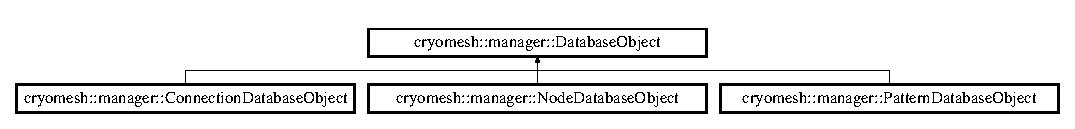
\includegraphics[height=1.287356cm]{classcryomesh_1_1manager_1_1DatabaseObject}
\end{center}
\end{figure}
\subsection*{\-Public \-Member \-Functions}
\begin{DoxyCompactItemize}
\item 
\hyperlink{classcryomesh_1_1manager_1_1DatabaseObject_a4806f6b018d86828c4251e06ac2634d9}{\-Database\-Object} ()
\item 
virtual \hyperlink{classcryomesh_1_1manager_1_1DatabaseObject_a462e3eeb0610dc1e7e47661b86c862f6}{$\sim$\-Database\-Object} ()
\item 
std\-::string \hyperlink{classcryomesh_1_1manager_1_1DatabaseObject_a66ded4e1a1bccd65c94922648c7135c5}{get\-Key} (const std\-::string \&key) const 
\begin{DoxyCompactList}\small\item\em \-Return the string object associated with a key. \end{DoxyCompactList}\item 
virtual std\-::string \hyperlink{classcryomesh_1_1manager_1_1DatabaseObject_ad55c6e711341a652790b97f549b0dc63}{get\-Insert} (const std\-::string \&table) const =0
\begin{DoxyCompactList}\small\item\em \-Get the string that can be used to insert the sql data. \end{DoxyCompactList}\end{DoxyCompactItemize}
\subsection*{\-Static \-Public \-Member \-Functions}
\begin{DoxyCompactItemize}
\item 
static std\-::string \hyperlink{classcryomesh_1_1manager_1_1DatabaseObject_aa4ef26ce91fea092f146e67add491e0f}{find\-Value} (const std\-::string \&entry, const std\-::map$<$ std\-::string, std\-::string $>$ \&map)
\begin{DoxyCompactList}\small\item\em \-Find entries value in map or return null. \end{DoxyCompactList}\item 
static std\-::map$<$ std\-::string, \*
std\-::string $>$ \hyperlink{classcryomesh_1_1manager_1_1DatabaseObject_a04ce7c34b51e3290c972121cf2f16565}{get\-Column\-Map\-From\-Entry} (const std\-::string \&entry)
\begin{DoxyCompactList}\small\item\em \-Parse a string database entry, extract columns and values and return a map. \end{DoxyCompactList}\item 
{\footnotesize template$<$class T $>$ }\\static std\-::string \hyperlink{classcryomesh_1_1manager_1_1DatabaseObject_a1b37d9d07009ae1c71f644761d36b468}{to\-String} (\-T obj)
\begin{DoxyCompactList}\small\item\em \-Convert an templated object that can be piped to a stream to a string. \end{DoxyCompactList}\end{DoxyCompactItemize}
\subsection*{\-Protected \-Attributes}
\begin{DoxyCompactItemize}
\item 
std\-::map$<$ std\-::string, \*
std\-::string $>$ \hyperlink{classcryomesh_1_1manager_1_1DatabaseObject_a9c648bf09b9fd8b4d599b0d4f4abf531}{columns}
\end{DoxyCompactItemize}


\subsection{\-Detailed \-Description}


\-Definition at line 21 of file \-Database\-Object.\-h.



\subsection{\-Constructor \& \-Destructor \-Documentation}
\hypertarget{classcryomesh_1_1manager_1_1DatabaseObject_a4806f6b018d86828c4251e06ac2634d9}{\index{cryomesh\-::manager\-::\-Database\-Object@{cryomesh\-::manager\-::\-Database\-Object}!\-Database\-Object@{\-Database\-Object}}
\index{\-Database\-Object@{\-Database\-Object}!cryomesh::manager::DatabaseObject@{cryomesh\-::manager\-::\-Database\-Object}}
\subsubsection[{\-Database\-Object}]{\setlength{\rightskip}{0pt plus 5cm}{\bf cryomesh\-::manager\-::\-Database\-Object\-::\-Database\-Object} (
\begin{DoxyParamCaption}
{}
\end{DoxyParamCaption}
)\hspace{0.3cm}{\ttfamily  \mbox{[}inline\mbox{]}}}}\label{classcryomesh_1_1manager_1_1DatabaseObject_a4806f6b018d86828c4251e06ac2634d9}


\-Definition at line 23 of file \-Database\-Object.\-h.

\hypertarget{classcryomesh_1_1manager_1_1DatabaseObject_a462e3eeb0610dc1e7e47661b86c862f6}{\index{cryomesh\-::manager\-::\-Database\-Object@{cryomesh\-::manager\-::\-Database\-Object}!$\sim$\-Database\-Object@{$\sim$\-Database\-Object}}
\index{$\sim$\-Database\-Object@{$\sim$\-Database\-Object}!cryomesh::manager::DatabaseObject@{cryomesh\-::manager\-::\-Database\-Object}}
\subsubsection[{$\sim$\-Database\-Object}]{\setlength{\rightskip}{0pt plus 5cm}virtual {\bf cryomesh\-::manager\-::\-Database\-Object\-::$\sim$\-Database\-Object} (
\begin{DoxyParamCaption}
{}
\end{DoxyParamCaption}
)\hspace{0.3cm}{\ttfamily  \mbox{[}inline, virtual\mbox{]}}}}\label{classcryomesh_1_1manager_1_1DatabaseObject_a462e3eeb0610dc1e7e47661b86c862f6}


\-Definition at line 25 of file \-Database\-Object.\-h.



\subsection{\-Member \-Function \-Documentation}
\hypertarget{classcryomesh_1_1manager_1_1DatabaseObject_aa4ef26ce91fea092f146e67add491e0f}{\index{cryomesh\-::manager\-::\-Database\-Object@{cryomesh\-::manager\-::\-Database\-Object}!find\-Value@{find\-Value}}
\index{find\-Value@{find\-Value}!cryomesh::manager::DatabaseObject@{cryomesh\-::manager\-::\-Database\-Object}}
\subsubsection[{find\-Value}]{\setlength{\rightskip}{0pt plus 5cm}static std\-::string {\bf cryomesh\-::manager\-::\-Database\-Object\-::find\-Value} (
\begin{DoxyParamCaption}
\item[{const std\-::string \&}]{entry, }
\item[{const std\-::map$<$ std\-::string, std\-::string $>$ \&}]{map}
\end{DoxyParamCaption}
)\hspace{0.3cm}{\ttfamily  \mbox{[}inline, static\mbox{]}}}}\label{classcryomesh_1_1manager_1_1DatabaseObject_aa4ef26ce91fea092f146e67add491e0f}


\-Find entries value in map or return null. 


\begin{DoxyParams}{\-Parameters}
{\em std\-::string} & \-Entry to find \\
\hline
{\em std\-::map$<$std\-::string,std\-::string} & map to search\\
\hline
\end{DoxyParams}
\begin{DoxyReturn}{\-Returns}
\-Value of entry 
\end{DoxyReturn}


\-Definition at line 59 of file \-Database\-Object.\-h.



\-Referenced by cryomesh\-::manager\-::\-Connection\-Database\-Object\-::\-Connection\-Database\-Object(), cryomesh\-::manager\-::\-Node\-Database\-Object\-::\-Node\-Database\-Object(), and cryomesh\-::manager\-::\-Pattern\-Database\-Object\-::\-Pattern\-Database\-Object().

\hypertarget{classcryomesh_1_1manager_1_1DatabaseObject_a04ce7c34b51e3290c972121cf2f16565}{\index{cryomesh\-::manager\-::\-Database\-Object@{cryomesh\-::manager\-::\-Database\-Object}!get\-Column\-Map\-From\-Entry@{get\-Column\-Map\-From\-Entry}}
\index{get\-Column\-Map\-From\-Entry@{get\-Column\-Map\-From\-Entry}!cryomesh::manager::DatabaseObject@{cryomesh\-::manager\-::\-Database\-Object}}
\subsubsection[{get\-Column\-Map\-From\-Entry}]{\setlength{\rightskip}{0pt plus 5cm}static std\-::map$<$std\-::string, std\-::string$>$ {\bf cryomesh\-::manager\-::\-Database\-Object\-::get\-Column\-Map\-From\-Entry} (
\begin{DoxyParamCaption}
\item[{const std\-::string \&}]{entry}
\end{DoxyParamCaption}
)\hspace{0.3cm}{\ttfamily  \mbox{[}inline, static\mbox{]}}}}\label{classcryomesh_1_1manager_1_1DatabaseObject_a04ce7c34b51e3290c972121cf2f16565}


\-Parse a string database entry, extract columns and values and return a map. 



\-Definition at line 72 of file \-Database\-Object.\-h.



\-Referenced by cryomesh\-::manager\-::\-Connection\-Database\-Object\-::\-Connection\-Database\-Object(), cryomesh\-::manager\-::\-Node\-Database\-Object\-::\-Node\-Database\-Object(), and cryomesh\-::manager\-::\-Pattern\-Database\-Object\-::\-Pattern\-Database\-Object().

\hypertarget{classcryomesh_1_1manager_1_1DatabaseObject_ad55c6e711341a652790b97f549b0dc63}{\index{cryomesh\-::manager\-::\-Database\-Object@{cryomesh\-::manager\-::\-Database\-Object}!get\-Insert@{get\-Insert}}
\index{get\-Insert@{get\-Insert}!cryomesh::manager::DatabaseObject@{cryomesh\-::manager\-::\-Database\-Object}}
\subsubsection[{get\-Insert}]{\setlength{\rightskip}{0pt plus 5cm}virtual std\-::string {\bf cryomesh\-::manager\-::\-Database\-Object\-::get\-Insert} (
\begin{DoxyParamCaption}
\item[{const std\-::string \&}]{table}
\end{DoxyParamCaption}
) const\hspace{0.3cm}{\ttfamily  \mbox{[}pure virtual\mbox{]}}}}\label{classcryomesh_1_1manager_1_1DatabaseObject_ad55c6e711341a652790b97f549b0dc63}


\-Get the string that can be used to insert the sql data. 

\begin{DoxyReturn}{\-Returns}
the sql command string to insert into this table 
\end{DoxyReturn}


\-Implemented in \hyperlink{classcryomesh_1_1manager_1_1ConnectionDatabaseObject_ac7b22d25a4366175fd7d1578f476b125}{cryomesh\-::manager\-::\-Connection\-Database\-Object}, \hyperlink{classcryomesh_1_1manager_1_1NodeDatabaseObject_ac5512082d08fa59cbaa496b711f4c8c2}{cryomesh\-::manager\-::\-Node\-Database\-Object}, and \hyperlink{classcryomesh_1_1manager_1_1PatternDatabaseObject_a0f4325cce7fd6c70017815ea50cd4fd6}{cryomesh\-::manager\-::\-Pattern\-Database\-Object}.



\-Referenced by cryomesh\-::manager\-::\-Database\-Manager\-::insert\-Connection(), cryomesh\-::manager\-::\-Database\-Manager\-::insert\-Node(), and cryomesh\-::manager\-::\-Database\-Manager\-::insert\-Output\-Pattern().

\hypertarget{classcryomesh_1_1manager_1_1DatabaseObject_a66ded4e1a1bccd65c94922648c7135c5}{\index{cryomesh\-::manager\-::\-Database\-Object@{cryomesh\-::manager\-::\-Database\-Object}!get\-Key@{get\-Key}}
\index{get\-Key@{get\-Key}!cryomesh::manager::DatabaseObject@{cryomesh\-::manager\-::\-Database\-Object}}
\subsubsection[{get\-Key}]{\setlength{\rightskip}{0pt plus 5cm}std\-::string {\bf cryomesh\-::manager\-::\-Database\-Object\-::get\-Key} (
\begin{DoxyParamCaption}
\item[{const std\-::string \&}]{key}
\end{DoxyParamCaption}
) const\hspace{0.3cm}{\ttfamily  \mbox{[}inline\mbox{]}}}}\label{classcryomesh_1_1manager_1_1DatabaseObject_a66ded4e1a1bccd65c94922648c7135c5}


\-Return the string object associated with a key. 

\-::string \-The key to search for

\begin{DoxyReturn}{\-Returns}
std\-::string \-The object associated with the search key, \char`\"{}\char`\"{} if not found 
\end{DoxyReturn}


\-Definition at line 37 of file \-Database\-Object.\-h.



\-References columns.



\-Referenced by cryomesh\-::manager\-::\-Pattern\-Database\-Object\-::get\-Insert(), cryomesh\-::manager\-::\-Node\-Database\-Object\-::get\-Insert(), and cryomesh\-::manager\-::\-Connection\-Database\-Object\-::get\-Insert().

\hypertarget{classcryomesh_1_1manager_1_1DatabaseObject_a1b37d9d07009ae1c71f644761d36b468}{\index{cryomesh\-::manager\-::\-Database\-Object@{cryomesh\-::manager\-::\-Database\-Object}!to\-String@{to\-String}}
\index{to\-String@{to\-String}!cryomesh::manager::DatabaseObject@{cryomesh\-::manager\-::\-Database\-Object}}
\subsubsection[{to\-String}]{\setlength{\rightskip}{0pt plus 5cm}template$<$class T $>$ static std\-::string {\bf cryomesh\-::manager\-::\-Database\-Object\-::to\-String} (
\begin{DoxyParamCaption}
\item[{\-T}]{obj}
\end{DoxyParamCaption}
)\hspace{0.3cm}{\ttfamily  \mbox{[}inline, static\mbox{]}}}}\label{classcryomesh_1_1manager_1_1DatabaseObject_a1b37d9d07009ae1c71f644761d36b468}


\-Convert an templated object that can be piped to a stream to a string. 


\begin{DoxyParams}{\-Parameters}
{\em \-T} & \-The object to get a string for \\
\hline
\end{DoxyParams}


\-Definition at line 108 of file \-Database\-Object.\-h.



\subsection{\-Member \-Data \-Documentation}
\hypertarget{classcryomesh_1_1manager_1_1DatabaseObject_a9c648bf09b9fd8b4d599b0d4f4abf531}{\index{cryomesh\-::manager\-::\-Database\-Object@{cryomesh\-::manager\-::\-Database\-Object}!columns@{columns}}
\index{columns@{columns}!cryomesh::manager::DatabaseObject@{cryomesh\-::manager\-::\-Database\-Object}}
\subsubsection[{columns}]{\setlength{\rightskip}{0pt plus 5cm}std\-::map$<$std\-::string, std\-::string$>$ {\bf cryomesh\-::manager\-::\-Database\-Object\-::columns}\hspace{0.3cm}{\ttfamily  \mbox{[}protected\mbox{]}}}}\label{classcryomesh_1_1manager_1_1DatabaseObject_a9c648bf09b9fd8b4d599b0d4f4abf531}


\-Definition at line 119 of file \-Database\-Object.\-h.



\-Referenced by cryomesh\-::manager\-::\-Connection\-Database\-Object\-::\-Connection\-Database\-Object(), get\-Key(), cryomesh\-::manager\-::\-Node\-Database\-Object\-::\-Node\-Database\-Object(), and cryomesh\-::manager\-::\-Pattern\-Database\-Object\-::\-Pattern\-Database\-Object().



\-The documentation for this class was generated from the following file\-:\begin{DoxyCompactItemize}
\item 
/home/niall/\-Projects/\-Eclipse/\-C\-P\-P/cryomesh/src/manager/\hyperlink{DatabaseObject_8h}{\-Database\-Object.\-h}\end{DoxyCompactItemize}

\hypertarget{classcryomesh_1_1dataobjects_1_1DataObject}{\section{cryomesh\-:\-:dataobjects\-:\-:\-Data\-Object$<$ \-U, \-T $>$ \-Class \-Template \-Reference}
\label{classcryomesh_1_1dataobjects_1_1DataObject}\index{cryomesh\-::dataobjects\-::\-Data\-Object$<$ U, T $>$@{cryomesh\-::dataobjects\-::\-Data\-Object$<$ U, T $>$}}
}


\-Class to contain all the useful data about an object.  




{\ttfamily \#include $<$\-Data\-Object.\-h$>$}

\subsection*{\-Public \-Types}
\begin{DoxyCompactItemize}
\item 
enum \hyperlink{classcryomesh_1_1dataobjects_1_1DataObject_a88c071e82534aa8b82c336a8104f9df8}{\-Comparison\-Type} \{ \hyperlink{classcryomesh_1_1dataobjects_1_1DataObject_a88c071e82534aa8b82c336a8104f9df8a00afa6fa8995597a48446b10044adc31}{\-Maximum\-Value}, 
\hyperlink{classcryomesh_1_1dataobjects_1_1DataObject_a88c071e82534aa8b82c336a8104f9df8adae0956c6e44c6d998d47407b6c1c9cd}{\-Minimum\-Value}, 
\hyperlink{classcryomesh_1_1dataobjects_1_1DataObject_a88c071e82534aa8b82c336a8104f9df8a9d1e58881794d424bd4759039d034741}{\-Equality\-Value}, 
\hyperlink{classcryomesh_1_1dataobjects_1_1DataObject_a88c071e82534aa8b82c336a8104f9df8abb8ba259cb26552c16f621c559f3e23d}{\-Average\-Value}
 \}
\begin{DoxyCompactList}\small\item\em \-Enum to signal the type of comparison to make. \end{DoxyCompactList}\end{DoxyCompactItemize}
\subsection*{\-Public \-Member \-Functions}
\begin{DoxyCompactItemize}
\item 
\hyperlink{classcryomesh_1_1dataobjects_1_1DataObject_a8be8493ecc93482b2ab10dc8c0a93440}{\-Data\-Object} ()
\begin{DoxyCompactList}\small\item\em \-Default contructor. \end{DoxyCompactList}\item 
\hyperlink{classcryomesh_1_1dataobjects_1_1DataObject_aff5302c3c41e16d4cc828d2bc3658cda}{\-Data\-Object} (unsigned int sz)
\begin{DoxyCompactList}\small\item\em \-Contructor with max size. \end{DoxyCompactList}\item 
virtual \hyperlink{classcryomesh_1_1dataobjects_1_1DataObject_a5542785b10e905eae83370406126830d}{$\sim$\-Data\-Object} ()
\begin{DoxyCompactList}\small\item\em \-Default destructor. \end{DoxyCompactList}\item 
void \hyperlink{classcryomesh_1_1dataobjects_1_1DataObject_a82e70f55cf4bff3c139a7aeaad4fc475}{enable\-Logging} (bool enable)
\begin{DoxyCompactList}\small\item\em \-Whether logging is enabled or not. \end{DoxyCompactList}\item 
bool \hyperlink{classcryomesh_1_1dataobjects_1_1DataObject_ac47906fb6abbb0e655e143b604255785}{is\-Logging\-Enabled} ()
\begin{DoxyCompactList}\small\item\em \-Check logging is enabled or not. \end{DoxyCompactList}\item 
const std\-::map$<$ \-U, \-T $>$ \& \hyperlink{classcryomesh_1_1dataobjects_1_1DataObject_a7b940ad5f397713567877b5295094fdd}{get\-Map} () const 
\begin{DoxyCompactList}\small\item\em \-Get all cycle values. \end{DoxyCompactList}\item 
std\-::map$<$ \-U, \-T $>$ \& \hyperlink{classcryomesh_1_1dataobjects_1_1DataObject_a52fe0b6b4106762a553875406ebd7023}{get\-Mutable\-Map} ()
\begin{DoxyCompactList}\small\item\em \-Get all mutable cycle values. \end{DoxyCompactList}\item 
const std\-::map$<$ \-U, \-T $>$ \hyperlink{classcryomesh_1_1dataobjects_1_1DataObject_a8e13c80d428064a1df4102da310c7836}{get\-Map} (\-U start, \-U end) const 
\begin{DoxyCompactList}\small\item\em \-Get all values within a range \mbox{[}start, end\mbox{]}. \end{DoxyCompactList}\item 
const std\-::map$<$ \-U, \-T $>$ \hyperlink{classcryomesh_1_1dataobjects_1_1DataObject_a04d86549f1cda29465e548fa3776fea6}{get\-Map} (\-U start) const 
\begin{DoxyCompactList}\small\item\em \-Get all values within a range \mbox{[}start, \mbox{]}. \end{DoxyCompactList}\item 
const \-T \hyperlink{classcryomesh_1_1dataobjects_1_1DataObject_a186b4e6a80bdf6a6d26c65e00c8aa547}{get\-By\-Key} (\-U key) const 
\begin{DoxyCompactList}\small\item\em \-Get value from key. \end{DoxyCompactList}\item 
void \hyperlink{classcryomesh_1_1dataobjects_1_1DataObject_a55ad9c772c8b174af40cbb530cf5fade}{clear} ()
\begin{DoxyCompactList}\small\item\em \-Clear all data. \end{DoxyCompactList}\item 
void \hyperlink{classcryomesh_1_1dataobjects_1_1DataObject_a7e57af8afd265116b13b027cc9ab6c52}{insert} (\-U key, \-T object)
\begin{DoxyCompactList}\small\item\em \-Add entry. \end{DoxyCompactList}\item 
unsigned int \hyperlink{classcryomesh_1_1dataobjects_1_1DataObject_a4b98ff0b286059f8c2cbe8277bfd3e02}{get\-Dataset\-Maximum\-Size} () const 
\item 
void \hyperlink{classcryomesh_1_1dataobjects_1_1DataObject_acdbdebc4d83ea9bde080ecf15a3ec6c6}{set\-Dataset\-Maximum\-Size} (unsigned int sz)
\item 
\-T \hyperlink{classcryomesh_1_1dataobjects_1_1DataObject_a1069d7cb1f2eb64c23d5eff7a5e15285}{get\-Value\-Comparison} (\hyperlink{classcryomesh_1_1dataobjects_1_1DataObject_a88c071e82534aa8b82c336a8104f9df8}{\-Comparison\-Type} type) const 
\begin{DoxyCompactList}\small\item\em \-Get comparison values. \end{DoxyCompactList}\item 
\-T \hyperlink{classcryomesh_1_1dataobjects_1_1DataObject_af92f3014a1406b596854b4b2fc9677a0}{get\-Maximum\-Value} () const 
\begin{DoxyCompactList}\small\item\em \-Get maximum value. \end{DoxyCompactList}\item 
\-T \hyperlink{classcryomesh_1_1dataobjects_1_1DataObject_a13afe46cb0349fba1a48636d34a46810}{get\-Minimum\-Value} () const 
\begin{DoxyCompactList}\small\item\em \-Get minimum value. \end{DoxyCompactList}\item 
\-T \hyperlink{classcryomesh_1_1dataobjects_1_1DataObject_ad1cd1f103cdaabb509abae7709cd8b09}{get\-Average\-Value} () const 
\begin{DoxyCompactList}\small\item\em \-Get average value value. \end{DoxyCompactList}\end{DoxyCompactItemize}
\subsection*{\-Protected \-Attributes}
\begin{DoxyCompactItemize}
\item 
std\-::map$<$ \-U, \-T $>$ \hyperlink{classcryomesh_1_1dataobjects_1_1DataObject_a9f345f10bea7d0554e09dbb4f598cd57}{value\-Map}
\item 
bool \hyperlink{classcryomesh_1_1dataobjects_1_1DataObject_a02128a10817ab449328375401f0199a9}{logging\-Enabled}
\item 
unsigned int \hyperlink{classcryomesh_1_1dataobjects_1_1DataObject_acec41108abc1ba2b1228e79bf14bb991}{dataset\-Maximum\-Size}
\end{DoxyCompactItemize}
\subsection*{\-Static \-Protected \-Attributes}
\begin{DoxyCompactItemize}
\item 
static const unsigned int \hyperlink{classcryomesh_1_1dataobjects_1_1DataObject_a493f002671f8c2d4db2b2a2953e434a0}{\-D\-E\-F\-A\-U\-L\-T\-\_\-\-D\-A\-T\-A\-S\-E\-T\-\_\-\-S\-I\-Z\-E} = 100
\end{DoxyCompactItemize}
\subsection*{\-Friends}
\begin{DoxyCompactItemize}
\item 
std\-::ostream \& \hyperlink{classcryomesh_1_1dataobjects_1_1DataObject_a71175025fe382ef063f84ad2281165aa}{operator$<$$<$} (std\-::ostream \&os, const \hyperlink{classcryomesh_1_1dataobjects_1_1DataObject}{\-Data\-Object} \&obj)
\begin{DoxyCompactList}\small\item\em \-To stream operator. \end{DoxyCompactList}\end{DoxyCompactItemize}


\subsection{\-Detailed \-Description}
\subsubsection*{template$<$class \-U, class \-T$>$class cryomesh\-::dataobjects\-::\-Data\-Object$<$ U, T $>$}

\-Class to contain all the useful data about an object. 

\-Useful for output and plotting 

\-Definition at line 22 of file \-Data\-Object.\-h.



\subsection{\-Member \-Enumeration \-Documentation}
\hypertarget{classcryomesh_1_1dataobjects_1_1DataObject_a88c071e82534aa8b82c336a8104f9df8}{\index{cryomesh\-::dataobjects\-::\-Data\-Object@{cryomesh\-::dataobjects\-::\-Data\-Object}!\-Comparison\-Type@{\-Comparison\-Type}}
\index{\-Comparison\-Type@{\-Comparison\-Type}!cryomesh::dataobjects::DataObject@{cryomesh\-::dataobjects\-::\-Data\-Object}}
\subsubsection[{\-Comparison\-Type}]{\setlength{\rightskip}{0pt plus 5cm}template$<$class \-U, class \-T$>$ enum {\bf cryomesh\-::dataobjects\-::\-Data\-Object}$<$ \-U, \-T $>$\-::{\bf \-Comparison\-Type}}}\label{classcryomesh_1_1dataobjects_1_1DataObject_a88c071e82534aa8b82c336a8104f9df8}


\-Enum to signal the type of comparison to make. 

\begin{Desc}
\item[\-Enumerator\-: ]\par
\begin{description}
\index{\-Maximum\-Value@{\-Maximum\-Value}!cryomesh\-::dataobjects\-::\-Data\-Object@{cryomesh\-::dataobjects\-::\-Data\-Object}}\index{cryomesh\-::dataobjects\-::\-Data\-Object@{cryomesh\-::dataobjects\-::\-Data\-Object}!\-Maximum\-Value@{\-Maximum\-Value}}\item[{\em 
\hypertarget{classcryomesh_1_1dataobjects_1_1DataObject_a88c071e82534aa8b82c336a8104f9df8a00afa6fa8995597a48446b10044adc31}{\-Maximum\-Value}\label{classcryomesh_1_1dataobjects_1_1DataObject_a88c071e82534aa8b82c336a8104f9df8a00afa6fa8995597a48446b10044adc31}
}]\index{\-Minimum\-Value@{\-Minimum\-Value}!cryomesh\-::dataobjects\-::\-Data\-Object@{cryomesh\-::dataobjects\-::\-Data\-Object}}\index{cryomesh\-::dataobjects\-::\-Data\-Object@{cryomesh\-::dataobjects\-::\-Data\-Object}!\-Minimum\-Value@{\-Minimum\-Value}}\item[{\em 
\hypertarget{classcryomesh_1_1dataobjects_1_1DataObject_a88c071e82534aa8b82c336a8104f9df8adae0956c6e44c6d998d47407b6c1c9cd}{\-Minimum\-Value}\label{classcryomesh_1_1dataobjects_1_1DataObject_a88c071e82534aa8b82c336a8104f9df8adae0956c6e44c6d998d47407b6c1c9cd}
}]\index{\-Equality\-Value@{\-Equality\-Value}!cryomesh\-::dataobjects\-::\-Data\-Object@{cryomesh\-::dataobjects\-::\-Data\-Object}}\index{cryomesh\-::dataobjects\-::\-Data\-Object@{cryomesh\-::dataobjects\-::\-Data\-Object}!\-Equality\-Value@{\-Equality\-Value}}\item[{\em 
\hypertarget{classcryomesh_1_1dataobjects_1_1DataObject_a88c071e82534aa8b82c336a8104f9df8a9d1e58881794d424bd4759039d034741}{\-Equality\-Value}\label{classcryomesh_1_1dataobjects_1_1DataObject_a88c071e82534aa8b82c336a8104f9df8a9d1e58881794d424bd4759039d034741}
}]\index{\-Average\-Value@{\-Average\-Value}!cryomesh\-::dataobjects\-::\-Data\-Object@{cryomesh\-::dataobjects\-::\-Data\-Object}}\index{cryomesh\-::dataobjects\-::\-Data\-Object@{cryomesh\-::dataobjects\-::\-Data\-Object}!\-Average\-Value@{\-Average\-Value}}\item[{\em 
\hypertarget{classcryomesh_1_1dataobjects_1_1DataObject_a88c071e82534aa8b82c336a8104f9df8abb8ba259cb26552c16f621c559f3e23d}{\-Average\-Value}\label{classcryomesh_1_1dataobjects_1_1DataObject_a88c071e82534aa8b82c336a8104f9df8abb8ba259cb26552c16f621c559f3e23d}
}]\end{description}
\end{Desc}



\-Definition at line 29 of file \-Data\-Object.\-h.



\subsection{\-Constructor \& \-Destructor \-Documentation}
\hypertarget{classcryomesh_1_1dataobjects_1_1DataObject_a8be8493ecc93482b2ab10dc8c0a93440}{\index{cryomesh\-::dataobjects\-::\-Data\-Object@{cryomesh\-::dataobjects\-::\-Data\-Object}!\-Data\-Object@{\-Data\-Object}}
\index{\-Data\-Object@{\-Data\-Object}!cryomesh::dataobjects::DataObject@{cryomesh\-::dataobjects\-::\-Data\-Object}}
\subsubsection[{\-Data\-Object}]{\setlength{\rightskip}{0pt plus 5cm}template$<$class \-U, class \-T$>$ {\bf cryomesh\-::dataobjects\-::\-Data\-Object}$<$ \-U, \-T $>$\-::{\bf \-Data\-Object} (
\begin{DoxyParamCaption}
{}
\end{DoxyParamCaption}
)\hspace{0.3cm}{\ttfamily  \mbox{[}inline\mbox{]}}}}\label{classcryomesh_1_1dataobjects_1_1DataObject_a8be8493ecc93482b2ab10dc8c0a93440}


\-Default contructor. 



\-Definition at line 36 of file \-Data\-Object.\-h.

\hypertarget{classcryomesh_1_1dataobjects_1_1DataObject_aff5302c3c41e16d4cc828d2bc3658cda}{\index{cryomesh\-::dataobjects\-::\-Data\-Object@{cryomesh\-::dataobjects\-::\-Data\-Object}!\-Data\-Object@{\-Data\-Object}}
\index{\-Data\-Object@{\-Data\-Object}!cryomesh::dataobjects::DataObject@{cryomesh\-::dataobjects\-::\-Data\-Object}}
\subsubsection[{\-Data\-Object}]{\setlength{\rightskip}{0pt plus 5cm}template$<$class \-U, class \-T$>$ {\bf cryomesh\-::dataobjects\-::\-Data\-Object}$<$ \-U, \-T $>$\-::{\bf \-Data\-Object} (
\begin{DoxyParamCaption}
\item[{unsigned int}]{sz}
\end{DoxyParamCaption}
)\hspace{0.3cm}{\ttfamily  \mbox{[}inline\mbox{]}}}}\label{classcryomesh_1_1dataobjects_1_1DataObject_aff5302c3c41e16d4cc828d2bc3658cda}


\-Contructor with max size. 


\begin{DoxyParams}{\-Parameters}
{\em unsigned} & int \-The maximum size of the data set \\
\hline
\end{DoxyParams}


\-Definition at line 46 of file \-Data\-Object.\-h.

\hypertarget{classcryomesh_1_1dataobjects_1_1DataObject_a5542785b10e905eae83370406126830d}{\index{cryomesh\-::dataobjects\-::\-Data\-Object@{cryomesh\-::dataobjects\-::\-Data\-Object}!$\sim$\-Data\-Object@{$\sim$\-Data\-Object}}
\index{$\sim$\-Data\-Object@{$\sim$\-Data\-Object}!cryomesh::dataobjects::DataObject@{cryomesh\-::dataobjects\-::\-Data\-Object}}
\subsubsection[{$\sim$\-Data\-Object}]{\setlength{\rightskip}{0pt plus 5cm}template$<$class \-U, class \-T$>$ virtual {\bf cryomesh\-::dataobjects\-::\-Data\-Object}$<$ \-U, \-T $>$\-::$\sim${\bf \-Data\-Object} (
\begin{DoxyParamCaption}
{}
\end{DoxyParamCaption}
)\hspace{0.3cm}{\ttfamily  \mbox{[}inline, virtual\mbox{]}}}}\label{classcryomesh_1_1dataobjects_1_1DataObject_a5542785b10e905eae83370406126830d}


\-Default destructor. 



\-Definition at line 53 of file \-Data\-Object.\-h.



\subsection{\-Member \-Function \-Documentation}
\hypertarget{classcryomesh_1_1dataobjects_1_1DataObject_a55ad9c772c8b174af40cbb530cf5fade}{\index{cryomesh\-::dataobjects\-::\-Data\-Object@{cryomesh\-::dataobjects\-::\-Data\-Object}!clear@{clear}}
\index{clear@{clear}!cryomesh::dataobjects::DataObject@{cryomesh\-::dataobjects\-::\-Data\-Object}}
\subsubsection[{clear}]{\setlength{\rightskip}{0pt plus 5cm}template$<$class \-U, class \-T$>$ void {\bf cryomesh\-::dataobjects\-::\-Data\-Object}$<$ \-U, \-T $>$\-::{\bf clear} (
\begin{DoxyParamCaption}
{}
\end{DoxyParamCaption}
)\hspace{0.3cm}{\ttfamily  \mbox{[}inline\mbox{]}}}}\label{classcryomesh_1_1dataobjects_1_1DataObject_a55ad9c772c8b174af40cbb530cf5fade}


\-Clear all data. 



\-Definition at line 178 of file \-Data\-Object.\-h.



\-Referenced by cryomesh\-::components\-::\-Impulse\-Collection\-::refresh\-Data\-Object().

\hypertarget{classcryomesh_1_1dataobjects_1_1DataObject_a82e70f55cf4bff3c139a7aeaad4fc475}{\index{cryomesh\-::dataobjects\-::\-Data\-Object@{cryomesh\-::dataobjects\-::\-Data\-Object}!enable\-Logging@{enable\-Logging}}
\index{enable\-Logging@{enable\-Logging}!cryomesh::dataobjects::DataObject@{cryomesh\-::dataobjects\-::\-Data\-Object}}
\subsubsection[{enable\-Logging}]{\setlength{\rightskip}{0pt plus 5cm}template$<$class \-U, class \-T$>$ void {\bf cryomesh\-::dataobjects\-::\-Data\-Object}$<$ \-U, \-T $>$\-::{\bf enable\-Logging} (
\begin{DoxyParamCaption}
\item[{bool}]{enable}
\end{DoxyParamCaption}
)\hspace{0.3cm}{\ttfamily  \mbox{[}inline\mbox{]}}}}\label{classcryomesh_1_1dataobjects_1_1DataObject_a82e70f55cf4bff3c139a7aeaad4fc475}


\-Whether logging is enabled or not. 


\begin{DoxyParams}{\-Parameters}
{\em bool} & enable \-True to enable logging, false otherwise \\
\hline
\end{DoxyParams}


\-Definition at line 62 of file \-Data\-Object.\-h.

\hypertarget{classcryomesh_1_1dataobjects_1_1DataObject_ad1cd1f103cdaabb509abae7709cd8b09}{\index{cryomesh\-::dataobjects\-::\-Data\-Object@{cryomesh\-::dataobjects\-::\-Data\-Object}!get\-Average\-Value@{get\-Average\-Value}}
\index{get\-Average\-Value@{get\-Average\-Value}!cryomesh::dataobjects::DataObject@{cryomesh\-::dataobjects\-::\-Data\-Object}}
\subsubsection[{get\-Average\-Value}]{\setlength{\rightskip}{0pt plus 5cm}template$<$class \-U, class \-T$>$ \-T {\bf cryomesh\-::dataobjects\-::\-Data\-Object}$<$ \-U, \-T $>$\-::{\bf get\-Average\-Value} (
\begin{DoxyParamCaption}
{}
\end{DoxyParamCaption}
) const\hspace{0.3cm}{\ttfamily  \mbox{[}inline\mbox{]}}}}\label{classcryomesh_1_1dataobjects_1_1DataObject_ad1cd1f103cdaabb509abae7709cd8b09}


\-Get average value value. 

\begin{DoxyReturn}{\-Returns}
\-T \-The resultant value 
\end{DoxyReturn}


\-Definition at line 283 of file \-Data\-Object.\-h.

\hypertarget{classcryomesh_1_1dataobjects_1_1DataObject_a186b4e6a80bdf6a6d26c65e00c8aa547}{\index{cryomesh\-::dataobjects\-::\-Data\-Object@{cryomesh\-::dataobjects\-::\-Data\-Object}!get\-By\-Key@{get\-By\-Key}}
\index{get\-By\-Key@{get\-By\-Key}!cryomesh::dataobjects::DataObject@{cryomesh\-::dataobjects\-::\-Data\-Object}}
\subsubsection[{get\-By\-Key}]{\setlength{\rightskip}{0pt plus 5cm}template$<$class \-U, class \-T$>$ const \-T {\bf cryomesh\-::dataobjects\-::\-Data\-Object}$<$ \-U, \-T $>$\-::{\bf get\-By\-Key} (
\begin{DoxyParamCaption}
\item[{\-U}]{key}
\end{DoxyParamCaption}
) const\hspace{0.3cm}{\ttfamily  \mbox{[}inline\mbox{]}}}}\label{classcryomesh_1_1dataobjects_1_1DataObject_a186b4e6a80bdf6a6d26c65e00c8aa547}


\-Get value from key. 


\begin{DoxyParams}{\-Parameters}
{\em \-U} & key \-The key to find\\
\hline
\end{DoxyParams}
\begin{DoxyReturn}{\-Returns}
\-T \-The value found 
\end{DoxyReturn}


\-Definition at line 138 of file \-Data\-Object.\-h.

\hypertarget{classcryomesh_1_1dataobjects_1_1DataObject_a4b98ff0b286059f8c2cbe8277bfd3e02}{\index{cryomesh\-::dataobjects\-::\-Data\-Object@{cryomesh\-::dataobjects\-::\-Data\-Object}!get\-Dataset\-Maximum\-Size@{get\-Dataset\-Maximum\-Size}}
\index{get\-Dataset\-Maximum\-Size@{get\-Dataset\-Maximum\-Size}!cryomesh::dataobjects::DataObject@{cryomesh\-::dataobjects\-::\-Data\-Object}}
\subsubsection[{get\-Dataset\-Maximum\-Size}]{\setlength{\rightskip}{0pt plus 5cm}template$<$class \-U, class \-T$>$ unsigned int {\bf cryomesh\-::dataobjects\-::\-Data\-Object}$<$ \-U, \-T $>$\-::{\bf get\-Dataset\-Maximum\-Size} (
\begin{DoxyParamCaption}
{}
\end{DoxyParamCaption}
) const\hspace{0.3cm}{\ttfamily  \mbox{[}inline\mbox{]}}}}\label{classcryomesh_1_1dataobjects_1_1DataObject_a4b98ff0b286059f8c2cbe8277bfd3e02}


\-Definition at line 212 of file \-Data\-Object.\-h.



\-Referenced by cryomesh\-::dataobjects\-::\-Data\-Object$<$ common\-::\-Cycle, double $>$\-::insert(), and cryomesh\-::components\-::\-Impulse\-Collection\-::refresh\-Data\-Object().

\hypertarget{classcryomesh_1_1dataobjects_1_1DataObject_a7b940ad5f397713567877b5295094fdd}{\index{cryomesh\-::dataobjects\-::\-Data\-Object@{cryomesh\-::dataobjects\-::\-Data\-Object}!get\-Map@{get\-Map}}
\index{get\-Map@{get\-Map}!cryomesh::dataobjects::DataObject@{cryomesh\-::dataobjects\-::\-Data\-Object}}
\subsubsection[{get\-Map}]{\setlength{\rightskip}{0pt plus 5cm}template$<$class \-U, class \-T$>$ const std\-::map$<$\-U, \-T$>$\& {\bf cryomesh\-::dataobjects\-::\-Data\-Object}$<$ \-U, \-T $>$\-::{\bf get\-Map} (
\begin{DoxyParamCaption}
{}
\end{DoxyParamCaption}
) const\hspace{0.3cm}{\ttfamily  \mbox{[}inline\mbox{]}}}}\label{classcryomesh_1_1dataobjects_1_1DataObject_a7b940ad5f397713567877b5295094fdd}


\-Get all cycle values. 

\begin{DoxyReturn}{\-Returns}
std\-::map$<$unsigned long int, double$>$ \& \-The cycle values 
\end{DoxyReturn}


\-Definition at line 81 of file \-Data\-Object.\-h.



\-Referenced by cryomesh\-::components\-::\-Node\-::get\-Activities().

\hypertarget{classcryomesh_1_1dataobjects_1_1DataObject_a8e13c80d428064a1df4102da310c7836}{\index{cryomesh\-::dataobjects\-::\-Data\-Object@{cryomesh\-::dataobjects\-::\-Data\-Object}!get\-Map@{get\-Map}}
\index{get\-Map@{get\-Map}!cryomesh::dataobjects::DataObject@{cryomesh\-::dataobjects\-::\-Data\-Object}}
\subsubsection[{get\-Map}]{\setlength{\rightskip}{0pt plus 5cm}template$<$class \-U, class \-T$>$ const std\-::map$<$\-U, \-T$>$ {\bf cryomesh\-::dataobjects\-::\-Data\-Object}$<$ \-U, \-T $>$\-::{\bf get\-Map} (
\begin{DoxyParamCaption}
\item[{\-U}]{start, }
\item[{\-U}]{end}
\end{DoxyParamCaption}
) const\hspace{0.3cm}{\ttfamily  \mbox{[}inline\mbox{]}}}}\label{classcryomesh_1_1dataobjects_1_1DataObject_a8e13c80d428064a1df4102da310c7836}


\-Get all values within a range \mbox{[}start, end\mbox{]}. 


\begin{DoxyParams}{\-Parameters}
{\em \-U} & start \-The start cycle of the range \\
\hline
{\em \-U} & end \-The end cycle of the range\\
\hline
\end{DoxyParams}
\begin{DoxyReturn}{\-Returns}
std\-::map$<$unsigned long int, double$>$ \-The cycle values 
\end{DoxyReturn}


\-Definition at line 106 of file \-Data\-Object.\-h.

\hypertarget{classcryomesh_1_1dataobjects_1_1DataObject_a04d86549f1cda29465e548fa3776fea6}{\index{cryomesh\-::dataobjects\-::\-Data\-Object@{cryomesh\-::dataobjects\-::\-Data\-Object}!get\-Map@{get\-Map}}
\index{get\-Map@{get\-Map}!cryomesh::dataobjects::DataObject@{cryomesh\-::dataobjects\-::\-Data\-Object}}
\subsubsection[{get\-Map}]{\setlength{\rightskip}{0pt plus 5cm}template$<$class \-U, class \-T$>$ const std\-::map$<$\-U, \-T$>$ {\bf cryomesh\-::dataobjects\-::\-Data\-Object}$<$ \-U, \-T $>$\-::{\bf get\-Map} (
\begin{DoxyParamCaption}
\item[{\-U}]{start}
\end{DoxyParamCaption}
) const\hspace{0.3cm}{\ttfamily  \mbox{[}inline\mbox{]}}}}\label{classcryomesh_1_1dataobjects_1_1DataObject_a04d86549f1cda29465e548fa3776fea6}


\-Get all values within a range \mbox{[}start, \mbox{]}. 


\begin{DoxyParams}{\-Parameters}
{\em \-U} & start \-The start cycle of the range\\
\hline
\end{DoxyParams}
\begin{DoxyReturn}{\-Returns}
std\-::map$<$unsigned long int, double$>$ \-The cycle values 
\end{DoxyReturn}


\-Definition at line 122 of file \-Data\-Object.\-h.

\hypertarget{classcryomesh_1_1dataobjects_1_1DataObject_af92f3014a1406b596854b4b2fc9677a0}{\index{cryomesh\-::dataobjects\-::\-Data\-Object@{cryomesh\-::dataobjects\-::\-Data\-Object}!get\-Maximum\-Value@{get\-Maximum\-Value}}
\index{get\-Maximum\-Value@{get\-Maximum\-Value}!cryomesh::dataobjects::DataObject@{cryomesh\-::dataobjects\-::\-Data\-Object}}
\subsubsection[{get\-Maximum\-Value}]{\setlength{\rightskip}{0pt plus 5cm}template$<$class \-U, class \-T$>$ \-T {\bf cryomesh\-::dataobjects\-::\-Data\-Object}$<$ \-U, \-T $>$\-::{\bf get\-Maximum\-Value} (
\begin{DoxyParamCaption}
{}
\end{DoxyParamCaption}
) const\hspace{0.3cm}{\ttfamily  \mbox{[}inline\mbox{]}}}}\label{classcryomesh_1_1dataobjects_1_1DataObject_af92f3014a1406b596854b4b2fc9677a0}


\-Get maximum value. 

\begin{DoxyReturn}{\-Returns}
\-T \-The resultant value 
\end{DoxyReturn}


\-Definition at line 263 of file \-Data\-Object.\-h.

\hypertarget{classcryomesh_1_1dataobjects_1_1DataObject_a13afe46cb0349fba1a48636d34a46810}{\index{cryomesh\-::dataobjects\-::\-Data\-Object@{cryomesh\-::dataobjects\-::\-Data\-Object}!get\-Minimum\-Value@{get\-Minimum\-Value}}
\index{get\-Minimum\-Value@{get\-Minimum\-Value}!cryomesh::dataobjects::DataObject@{cryomesh\-::dataobjects\-::\-Data\-Object}}
\subsubsection[{get\-Minimum\-Value}]{\setlength{\rightskip}{0pt plus 5cm}template$<$class \-U, class \-T$>$ \-T {\bf cryomesh\-::dataobjects\-::\-Data\-Object}$<$ \-U, \-T $>$\-::{\bf get\-Minimum\-Value} (
\begin{DoxyParamCaption}
{}
\end{DoxyParamCaption}
) const\hspace{0.3cm}{\ttfamily  \mbox{[}inline\mbox{]}}}}\label{classcryomesh_1_1dataobjects_1_1DataObject_a13afe46cb0349fba1a48636d34a46810}


\-Get minimum value. 

\begin{DoxyReturn}{\-Returns}
\-T \-The resultant value 
\end{DoxyReturn}


\-Definition at line 273 of file \-Data\-Object.\-h.

\hypertarget{classcryomesh_1_1dataobjects_1_1DataObject_a52fe0b6b4106762a553875406ebd7023}{\index{cryomesh\-::dataobjects\-::\-Data\-Object@{cryomesh\-::dataobjects\-::\-Data\-Object}!get\-Mutable\-Map@{get\-Mutable\-Map}}
\index{get\-Mutable\-Map@{get\-Mutable\-Map}!cryomesh::dataobjects::DataObject@{cryomesh\-::dataobjects\-::\-Data\-Object}}
\subsubsection[{get\-Mutable\-Map}]{\setlength{\rightskip}{0pt plus 5cm}template$<$class \-U, class \-T$>$ std\-::map$<$\-U, \-T$>$\& {\bf cryomesh\-::dataobjects\-::\-Data\-Object}$<$ \-U, \-T $>$\-::{\bf get\-Mutable\-Map} (
\begin{DoxyParamCaption}
{}
\end{DoxyParamCaption}
)\hspace{0.3cm}{\ttfamily  \mbox{[}inline\mbox{]}}}}\label{classcryomesh_1_1dataobjects_1_1DataObject_a52fe0b6b4106762a553875406ebd7023}


\-Get all mutable cycle values. 

\begin{DoxyReturn}{\-Returns}
std\-::map$<$\-U, T$>$ \& \-The mutable cycle values 
\end{DoxyReturn}


\-Definition at line 91 of file \-Data\-Object.\-h.

\hypertarget{classcryomesh_1_1dataobjects_1_1DataObject_a1069d7cb1f2eb64c23d5eff7a5e15285}{\index{cryomesh\-::dataobjects\-::\-Data\-Object@{cryomesh\-::dataobjects\-::\-Data\-Object}!get\-Value\-Comparison@{get\-Value\-Comparison}}
\index{get\-Value\-Comparison@{get\-Value\-Comparison}!cryomesh::dataobjects::DataObject@{cryomesh\-::dataobjects\-::\-Data\-Object}}
\subsubsection[{get\-Value\-Comparison}]{\setlength{\rightskip}{0pt plus 5cm}template$<$class \-U, class \-T$>$ \-T {\bf cryomesh\-::dataobjects\-::\-Data\-Object}$<$ \-U, \-T $>$\-::{\bf get\-Value\-Comparison} (
\begin{DoxyParamCaption}
\item[{{\bf \-Comparison\-Type}}]{type}
\end{DoxyParamCaption}
) const\hspace{0.3cm}{\ttfamily  \mbox{[}inline\mbox{]}}}}\label{classcryomesh_1_1dataobjects_1_1DataObject_a1069d7cb1f2eb64c23d5eff7a5e15285}


\-Get comparison values. 


\begin{DoxyParams}{\-Parameters}
{\em \-Comparison\-Type} & type \-The type of comparison to make\\
\hline
\end{DoxyParams}
\begin{DoxyReturn}{\-Returns}
\-T \-The result of the comparison 
\end{DoxyReturn}


\-Definition at line 229 of file \-Data\-Object.\-h.



\-Referenced by cryomesh\-::dataobjects\-::\-Data\-Object$<$ common\-::\-Cycle, double $>$\-::get\-Average\-Value(), cryomesh\-::dataobjects\-::\-Data\-Object$<$ common\-::\-Cycle, double $>$\-::get\-Maximum\-Value(), and cryomesh\-::dataobjects\-::\-Data\-Object$<$ common\-::\-Cycle, double $>$\-::get\-Minimum\-Value().

\hypertarget{classcryomesh_1_1dataobjects_1_1DataObject_a7e57af8afd265116b13b027cc9ab6c52}{\index{cryomesh\-::dataobjects\-::\-Data\-Object@{cryomesh\-::dataobjects\-::\-Data\-Object}!insert@{insert}}
\index{insert@{insert}!cryomesh::dataobjects::DataObject@{cryomesh\-::dataobjects\-::\-Data\-Object}}
\subsubsection[{insert}]{\setlength{\rightskip}{0pt plus 5cm}template$<$class \-U, class \-T$>$ void {\bf cryomesh\-::dataobjects\-::\-Data\-Object}$<$ \-U, \-T $>$\-::{\bf insert} (
\begin{DoxyParamCaption}
\item[{\-U}]{key, }
\item[{\-T}]{object}
\end{DoxyParamCaption}
)\hspace{0.3cm}{\ttfamily  \mbox{[}inline\mbox{]}}}}\label{classcryomesh_1_1dataobjects_1_1DataObject_a7e57af8afd265116b13b027cc9ab6c52}


\-Add entry. 


\begin{DoxyParams}{\-Parameters}
{\em unsigned} & int cycle \-The cycle the value is on \\
\hline
{\em double} & \-The value \\
\hline
\end{DoxyParams}


\-Definition at line 191 of file \-Data\-Object.\-h.



\-Referenced by cryomesh\-::components\-::\-Node\-::add\-Activity(), cryomesh\-::components\-::\-Impulse\-Collection\-::refresh\-Data\-Object(), and cryomesh\-::components\-::\-Node\-::update().

\hypertarget{classcryomesh_1_1dataobjects_1_1DataObject_ac47906fb6abbb0e655e143b604255785}{\index{cryomesh\-::dataobjects\-::\-Data\-Object@{cryomesh\-::dataobjects\-::\-Data\-Object}!is\-Logging\-Enabled@{is\-Logging\-Enabled}}
\index{is\-Logging\-Enabled@{is\-Logging\-Enabled}!cryomesh::dataobjects::DataObject@{cryomesh\-::dataobjects\-::\-Data\-Object}}
\subsubsection[{is\-Logging\-Enabled}]{\setlength{\rightskip}{0pt plus 5cm}template$<$class \-U, class \-T$>$ bool {\bf cryomesh\-::dataobjects\-::\-Data\-Object}$<$ \-U, \-T $>$\-::{\bf is\-Logging\-Enabled} (
\begin{DoxyParamCaption}
{}
\end{DoxyParamCaption}
)\hspace{0.3cm}{\ttfamily  \mbox{[}inline\mbox{]}}}}\label{classcryomesh_1_1dataobjects_1_1DataObject_ac47906fb6abbb0e655e143b604255785}


\-Check logging is enabled or not. 

\begin{DoxyReturn}{\-Returns}
bool enable \-Trueif logging enabled, flase otherwise 
\end{DoxyReturn}


\-Definition at line 71 of file \-Data\-Object.\-h.



\-Referenced by cryomesh\-::components\-::\-Impulse\-Collection\-::refresh\-Data\-Object(), and cryomesh\-::components\-::\-Node\-::update().

\hypertarget{classcryomesh_1_1dataobjects_1_1DataObject_acdbdebc4d83ea9bde080ecf15a3ec6c6}{\index{cryomesh\-::dataobjects\-::\-Data\-Object@{cryomesh\-::dataobjects\-::\-Data\-Object}!set\-Dataset\-Maximum\-Size@{set\-Dataset\-Maximum\-Size}}
\index{set\-Dataset\-Maximum\-Size@{set\-Dataset\-Maximum\-Size}!cryomesh::dataobjects::DataObject@{cryomesh\-::dataobjects\-::\-Data\-Object}}
\subsubsection[{set\-Dataset\-Maximum\-Size}]{\setlength{\rightskip}{0pt plus 5cm}template$<$class \-U, class \-T$>$ void {\bf cryomesh\-::dataobjects\-::\-Data\-Object}$<$ \-U, \-T $>$\-::{\bf set\-Dataset\-Maximum\-Size} (
\begin{DoxyParamCaption}
\item[{unsigned int}]{sz}
\end{DoxyParamCaption}
)\hspace{0.3cm}{\ttfamily  \mbox{[}inline\mbox{]}}}}\label{classcryomesh_1_1dataobjects_1_1DataObject_acdbdebc4d83ea9bde080ecf15a3ec6c6}


\-Definition at line 216 of file \-Data\-Object.\-h.



\-Referenced by cryomesh\-::components\-::\-Node\-::\-Node().



\subsection{\-Friends \-And \-Related \-Function \-Documentation}
\hypertarget{classcryomesh_1_1dataobjects_1_1DataObject_a71175025fe382ef063f84ad2281165aa}{\index{cryomesh\-::dataobjects\-::\-Data\-Object@{cryomesh\-::dataobjects\-::\-Data\-Object}!operator$<$$<$@{operator$<$$<$}}
\index{operator$<$$<$@{operator$<$$<$}!cryomesh::dataobjects::DataObject@{cryomesh\-::dataobjects\-::\-Data\-Object}}
\subsubsection[{operator$<$$<$}]{\setlength{\rightskip}{0pt plus 5cm}template$<$class \-U, class \-T$>$ std\-::ostream\& operator$<$$<$ (
\begin{DoxyParamCaption}
\item[{std\-::ostream \&}]{os, }
\item[{const {\bf \-Data\-Object}$<$ \-U, \-T $>$ \&}]{obj}
\end{DoxyParamCaption}
)\hspace{0.3cm}{\ttfamily  \mbox{[}friend\mbox{]}}}}\label{classcryomesh_1_1dataobjects_1_1DataObject_a71175025fe382ef063f84ad2281165aa}


\-To stream operator. 


\begin{DoxyParams}{\-Parameters}
{\em std\-::ostream} & \& os \-The output stream \\
\hline
{\em const} & \hyperlink{classcryomesh_1_1dataobjects_1_1DataObject}{\-Data\-Object} \& obj \-The object to stream\\
\hline
\end{DoxyParams}
\begin{DoxyReturn}{\-Returns}
std\-::ostream \& \-The output stream 
\end{DoxyReturn}


\-Definition at line 159 of file \-Data\-Object.\-h.



\subsection{\-Member \-Data \-Documentation}
\hypertarget{classcryomesh_1_1dataobjects_1_1DataObject_acec41108abc1ba2b1228e79bf14bb991}{\index{cryomesh\-::dataobjects\-::\-Data\-Object@{cryomesh\-::dataobjects\-::\-Data\-Object}!dataset\-Maximum\-Size@{dataset\-Maximum\-Size}}
\index{dataset\-Maximum\-Size@{dataset\-Maximum\-Size}!cryomesh::dataobjects::DataObject@{cryomesh\-::dataobjects\-::\-Data\-Object}}
\subsubsection[{dataset\-Maximum\-Size}]{\setlength{\rightskip}{0pt plus 5cm}template$<$class \-U, class \-T$>$ unsigned int {\bf cryomesh\-::dataobjects\-::\-Data\-Object}$<$ \-U, \-T $>$\-::{\bf dataset\-Maximum\-Size}\hspace{0.3cm}{\ttfamily  \mbox{[}protected\mbox{]}}}}\label{classcryomesh_1_1dataobjects_1_1DataObject_acec41108abc1ba2b1228e79bf14bb991}


\-Definition at line 306 of file \-Data\-Object.\-h.



\-Referenced by cryomesh\-::dataobjects\-::\-Data\-Object$<$ common\-::\-Cycle, double $>$\-::get\-Dataset\-Maximum\-Size(), and cryomesh\-::dataobjects\-::\-Data\-Object$<$ common\-::\-Cycle, double $>$\-::set\-Dataset\-Maximum\-Size().

\hypertarget{classcryomesh_1_1dataobjects_1_1DataObject_a493f002671f8c2d4db2b2a2953e434a0}{\index{cryomesh\-::dataobjects\-::\-Data\-Object@{cryomesh\-::dataobjects\-::\-Data\-Object}!\-D\-E\-F\-A\-U\-L\-T\-\_\-\-D\-A\-T\-A\-S\-E\-T\-\_\-\-S\-I\-Z\-E@{\-D\-E\-F\-A\-U\-L\-T\-\_\-\-D\-A\-T\-A\-S\-E\-T\-\_\-\-S\-I\-Z\-E}}
\index{\-D\-E\-F\-A\-U\-L\-T\-\_\-\-D\-A\-T\-A\-S\-E\-T\-\_\-\-S\-I\-Z\-E@{\-D\-E\-F\-A\-U\-L\-T\-\_\-\-D\-A\-T\-A\-S\-E\-T\-\_\-\-S\-I\-Z\-E}!cryomesh::dataobjects::DataObject@{cryomesh\-::dataobjects\-::\-Data\-Object}}
\subsubsection[{\-D\-E\-F\-A\-U\-L\-T\-\_\-\-D\-A\-T\-A\-S\-E\-T\-\_\-\-S\-I\-Z\-E}]{\setlength{\rightskip}{0pt plus 5cm}template$<$class \-U, class \-T$>$ const unsigned int {\bf cryomesh\-::dataobjects\-::\-Data\-Object}$<$ \-U, \-T $>$\-::{\bf \-D\-E\-F\-A\-U\-L\-T\-\_\-\-D\-A\-T\-A\-S\-E\-T\-\_\-\-S\-I\-Z\-E} = 100\hspace{0.3cm}{\ttfamily  \mbox{[}static, protected\mbox{]}}}}\label{classcryomesh_1_1dataobjects_1_1DataObject_a493f002671f8c2d4db2b2a2953e434a0}


\-Definition at line 313 of file \-Data\-Object.\-h.

\hypertarget{classcryomesh_1_1dataobjects_1_1DataObject_a02128a10817ab449328375401f0199a9}{\index{cryomesh\-::dataobjects\-::\-Data\-Object@{cryomesh\-::dataobjects\-::\-Data\-Object}!logging\-Enabled@{logging\-Enabled}}
\index{logging\-Enabled@{logging\-Enabled}!cryomesh::dataobjects::DataObject@{cryomesh\-::dataobjects\-::\-Data\-Object}}
\subsubsection[{logging\-Enabled}]{\setlength{\rightskip}{0pt plus 5cm}template$<$class \-U, class \-T$>$ bool {\bf cryomesh\-::dataobjects\-::\-Data\-Object}$<$ \-U, \-T $>$\-::{\bf logging\-Enabled}\hspace{0.3cm}{\ttfamily  \mbox{[}protected\mbox{]}}}}\label{classcryomesh_1_1dataobjects_1_1DataObject_a02128a10817ab449328375401f0199a9}


\-Definition at line 299 of file \-Data\-Object.\-h.



\-Referenced by cryomesh\-::dataobjects\-::\-Data\-Object$<$ common\-::\-Cycle, double $>$\-::enable\-Logging(), and cryomesh\-::dataobjects\-::\-Data\-Object$<$ common\-::\-Cycle, double $>$\-::is\-Logging\-Enabled().

\hypertarget{classcryomesh_1_1dataobjects_1_1DataObject_a9f345f10bea7d0554e09dbb4f598cd57}{\index{cryomesh\-::dataobjects\-::\-Data\-Object@{cryomesh\-::dataobjects\-::\-Data\-Object}!value\-Map@{value\-Map}}
\index{value\-Map@{value\-Map}!cryomesh::dataobjects::DataObject@{cryomesh\-::dataobjects\-::\-Data\-Object}}
\subsubsection[{value\-Map}]{\setlength{\rightskip}{0pt plus 5cm}template$<$class \-U, class \-T$>$ std\-::map$<$\-U, \-T$>$ {\bf cryomesh\-::dataobjects\-::\-Data\-Object}$<$ \-U, \-T $>$\-::{\bf value\-Map}\hspace{0.3cm}{\ttfamily  \mbox{[}protected\mbox{]}}}}\label{classcryomesh_1_1dataobjects_1_1DataObject_a9f345f10bea7d0554e09dbb4f598cd57}


\-Definition at line 292 of file \-Data\-Object.\-h.



\-Referenced by cryomesh\-::dataobjects\-::\-Data\-Object$<$ common\-::\-Cycle, double $>$\-::clear(), cryomesh\-::dataobjects\-::\-Data\-Object$<$ common\-::\-Cycle, double $>$\-::get\-By\-Key(), cryomesh\-::dataobjects\-::\-Data\-Object$<$ common\-::\-Cycle, double $>$\-::get\-Map(), cryomesh\-::dataobjects\-::\-Data\-Object$<$ common\-::\-Cycle, double $>$\-::get\-Mutable\-Map(), cryomesh\-::dataobjects\-::\-Data\-Object$<$ common\-::\-Cycle, double $>$\-::get\-Value\-Comparison(), and cryomesh\-::dataobjects\-::\-Data\-Object$<$ common\-::\-Cycle, double $>$\-::insert().



\-The documentation for this class was generated from the following file\-:\begin{DoxyCompactItemize}
\item 
/home/niall/\-Projects/\-Eclipse/\-C\-P\-P/cryomesh/src/dataobjects/\hyperlink{DataObject_8h}{\-Data\-Object.\-h}\end{DoxyCompactItemize}

\hypertarget{classcryomesh_1_1dataobjects_1_1DataObjectController}{\section{cryomesh\-:\-:dataobjects\-:\-:\-Data\-Object\-Controller$<$ \-U, \-T $>$ \-Class \-Template \-Reference}
\label{classcryomesh_1_1dataobjects_1_1DataObjectController}\index{cryomesh\-::dataobjects\-::\-Data\-Object\-Controller$<$ U, T $>$@{cryomesh\-::dataobjects\-::\-Data\-Object\-Controller$<$ U, T $>$}}
}


\-Class used to interface with data objects.  




{\ttfamily \#include $<$\-Data\-Object\-Controller.\-h$>$}

\subsection*{\-Public \-Member \-Functions}
\begin{DoxyCompactItemize}
\item 
\hyperlink{classcryomesh_1_1dataobjects_1_1DataObjectController_a9b5dd38c83c6fb1dc5bcf4ddcbc7a577}{\-Data\-Object\-Controller} ()
\begin{DoxyCompactList}\small\item\em \-Default constructor. \end{DoxyCompactList}\item 
\hyperlink{classcryomesh_1_1dataobjects_1_1DataObjectController_a01e98fc9bc0f3495bd05e01e6cc15f29}{\-Data\-Object\-Controller} (unsigned int sz)
\begin{DoxyCompactList}\small\item\em \-Contructor with size. \end{DoxyCompactList}\item 
virtual \hyperlink{classcryomesh_1_1dataobjects_1_1DataObjectController_aa023e2b5199e935b52781a8556d97cbe}{$\sim$\-Data\-Object\-Controller} ()
\item 
virtual void \hyperlink{classcryomesh_1_1dataobjects_1_1DataObjectController_a3e510413675407ec0a6745345ca9a3a8}{enable\-Logging} (bool enable)
\begin{DoxyCompactList}\small\item\em \-Whether logging is enabled or not. \end{DoxyCompactList}\item 
virtual const std\-::map$<$ \-U, \-T $>$ \& \hyperlink{classcryomesh_1_1dataobjects_1_1DataObjectController_a70a03ee28392ecf2e039702a18511f05}{get\-Map} ()
\begin{DoxyCompactList}\small\item\em \-Get all cycle values. \end{DoxyCompactList}\item 
virtual const \*
\hyperlink{classcryomesh_1_1dataobjects_1_1DataObject}{dataobjects\-::\-Data\-Object}$<$ \-U, \-T $>$ \& \hyperlink{classcryomesh_1_1dataobjects_1_1DataObjectController_aa919e8676a611028c6b6e6791c87f438}{get\-Data\-Object} ()
\begin{DoxyCompactList}\small\item\em \-Get data object. \end{DoxyCompactList}\item 
virtual void \hyperlink{classcryomesh_1_1dataobjects_1_1DataObjectController_ae015efe3d10cced82d5043f560cbe04f}{refresh\-Data\-Object} ()
\begin{DoxyCompactList}\small\item\em \-Function to allow refreshing implementation if required by subclasses. \end{DoxyCompactList}\end{DoxyCompactItemize}
\subsection*{\-Protected \-Attributes}
\begin{DoxyCompactItemize}
\item 
\hyperlink{classcryomesh_1_1dataobjects_1_1DataObject}{dataobjects\-::\-Data\-Object}$<$ \-U, \-T $>$ \hyperlink{classcryomesh_1_1dataobjects_1_1DataObjectController_aa13d30e9fa2f1caa0510635214d4bb26}{data\-Object}
\end{DoxyCompactItemize}


\subsection{\-Detailed \-Description}
\subsubsection*{template$<$class \-U, class \-T$>$class cryomesh\-::dataobjects\-::\-Data\-Object\-Controller$<$ U, T $>$}

\-Class used to interface with data objects. 

\-Definition at line 21 of file \-Data\-Object\-Controller.\-h.



\subsection{\-Constructor \& \-Destructor \-Documentation}
\hypertarget{classcryomesh_1_1dataobjects_1_1DataObjectController_a9b5dd38c83c6fb1dc5bcf4ddcbc7a577}{\index{cryomesh\-::dataobjects\-::\-Data\-Object\-Controller@{cryomesh\-::dataobjects\-::\-Data\-Object\-Controller}!\-Data\-Object\-Controller@{\-Data\-Object\-Controller}}
\index{\-Data\-Object\-Controller@{\-Data\-Object\-Controller}!cryomesh::dataobjects::DataObjectController@{cryomesh\-::dataobjects\-::\-Data\-Object\-Controller}}
\subsubsection[{\-Data\-Object\-Controller}]{\setlength{\rightskip}{0pt plus 5cm}template$<$class \-U, class \-T$>$ {\bf cryomesh\-::dataobjects\-::\-Data\-Object\-Controller}$<$ \-U, \-T $>$\-::{\bf \-Data\-Object\-Controller} (
\begin{DoxyParamCaption}
{}
\end{DoxyParamCaption}
)\hspace{0.3cm}{\ttfamily  \mbox{[}inline\mbox{]}}}}\label{classcryomesh_1_1dataobjects_1_1DataObjectController_a9b5dd38c83c6fb1dc5bcf4ddcbc7a577}


\-Default constructor. 



\-Definition at line 27 of file \-Data\-Object\-Controller.\-h.

\hypertarget{classcryomesh_1_1dataobjects_1_1DataObjectController_a01e98fc9bc0f3495bd05e01e6cc15f29}{\index{cryomesh\-::dataobjects\-::\-Data\-Object\-Controller@{cryomesh\-::dataobjects\-::\-Data\-Object\-Controller}!\-Data\-Object\-Controller@{\-Data\-Object\-Controller}}
\index{\-Data\-Object\-Controller@{\-Data\-Object\-Controller}!cryomesh::dataobjects::DataObjectController@{cryomesh\-::dataobjects\-::\-Data\-Object\-Controller}}
\subsubsection[{\-Data\-Object\-Controller}]{\setlength{\rightskip}{0pt plus 5cm}template$<$class \-U, class \-T$>$ {\bf cryomesh\-::dataobjects\-::\-Data\-Object\-Controller}$<$ \-U, \-T $>$\-::{\bf \-Data\-Object\-Controller} (
\begin{DoxyParamCaption}
\item[{unsigned int}]{sz}
\end{DoxyParamCaption}
)\hspace{0.3cm}{\ttfamily  \mbox{[}inline\mbox{]}}}}\label{classcryomesh_1_1dataobjects_1_1DataObjectController_a01e98fc9bc0f3495bd05e01e6cc15f29}


\-Contructor with size. 


\begin{DoxyParams}{\-Parameters}
{\em unsigned} & int \-The maximum size of the data set \\
\hline
\end{DoxyParams}


\-Definition at line 36 of file \-Data\-Object\-Controller.\-h.

\hypertarget{classcryomesh_1_1dataobjects_1_1DataObjectController_aa023e2b5199e935b52781a8556d97cbe}{\index{cryomesh\-::dataobjects\-::\-Data\-Object\-Controller@{cryomesh\-::dataobjects\-::\-Data\-Object\-Controller}!$\sim$\-Data\-Object\-Controller@{$\sim$\-Data\-Object\-Controller}}
\index{$\sim$\-Data\-Object\-Controller@{$\sim$\-Data\-Object\-Controller}!cryomesh::dataobjects::DataObjectController@{cryomesh\-::dataobjects\-::\-Data\-Object\-Controller}}
\subsubsection[{$\sim$\-Data\-Object\-Controller}]{\setlength{\rightskip}{0pt plus 5cm}template$<$class \-U, class \-T$>$ virtual {\bf cryomesh\-::dataobjects\-::\-Data\-Object\-Controller}$<$ \-U, \-T $>$\-::$\sim${\bf \-Data\-Object\-Controller} (
\begin{DoxyParamCaption}
{}
\end{DoxyParamCaption}
)\hspace{0.3cm}{\ttfamily  \mbox{[}inline, virtual\mbox{]}}}}\label{classcryomesh_1_1dataobjects_1_1DataObjectController_aa023e2b5199e935b52781a8556d97cbe}


\-Definition at line 39 of file \-Data\-Object\-Controller.\-h.



\subsection{\-Member \-Function \-Documentation}
\hypertarget{classcryomesh_1_1dataobjects_1_1DataObjectController_a3e510413675407ec0a6745345ca9a3a8}{\index{cryomesh\-::dataobjects\-::\-Data\-Object\-Controller@{cryomesh\-::dataobjects\-::\-Data\-Object\-Controller}!enable\-Logging@{enable\-Logging}}
\index{enable\-Logging@{enable\-Logging}!cryomesh::dataobjects::DataObjectController@{cryomesh\-::dataobjects\-::\-Data\-Object\-Controller}}
\subsubsection[{enable\-Logging}]{\setlength{\rightskip}{0pt plus 5cm}template$<$class \-U, class \-T$>$ virtual void {\bf cryomesh\-::dataobjects\-::\-Data\-Object\-Controller}$<$ \-U, \-T $>$\-::{\bf enable\-Logging} (
\begin{DoxyParamCaption}
\item[{bool}]{enable}
\end{DoxyParamCaption}
)\hspace{0.3cm}{\ttfamily  \mbox{[}inline, virtual\mbox{]}}}}\label{classcryomesh_1_1dataobjects_1_1DataObjectController_a3e510413675407ec0a6745345ca9a3a8}


\-Whether logging is enabled or not. 


\begin{DoxyParams}{\-Parameters}
{\em bool} & enable \-True to enable logging, false otherwise \\
\hline
\end{DoxyParams}


\-Definition at line 47 of file \-Data\-Object\-Controller.\-h.

\hypertarget{classcryomesh_1_1dataobjects_1_1DataObjectController_aa919e8676a611028c6b6e6791c87f438}{\index{cryomesh\-::dataobjects\-::\-Data\-Object\-Controller@{cryomesh\-::dataobjects\-::\-Data\-Object\-Controller}!get\-Data\-Object@{get\-Data\-Object}}
\index{get\-Data\-Object@{get\-Data\-Object}!cryomesh::dataobjects::DataObjectController@{cryomesh\-::dataobjects\-::\-Data\-Object\-Controller}}
\subsubsection[{get\-Data\-Object}]{\setlength{\rightskip}{0pt plus 5cm}template$<$class \-U, class \-T$>$ virtual const {\bf dataobjects\-::\-Data\-Object}$<$\-U, \-T$>$\& {\bf cryomesh\-::dataobjects\-::\-Data\-Object\-Controller}$<$ \-U, \-T $>$\-::{\bf get\-Data\-Object} (
\begin{DoxyParamCaption}
{}
\end{DoxyParamCaption}
)\hspace{0.3cm}{\ttfamily  \mbox{[}inline, virtual\mbox{]}}}}\label{classcryomesh_1_1dataobjects_1_1DataObjectController_aa919e8676a611028c6b6e6791c87f438}


\-Get data object. 

\begin{DoxyReturn}{\-Returns}
dataobjects\-::\-Data\-Object$<$\-U,\-T$>$ \& \-The data object 
\end{DoxyReturn}


\-Definition at line 68 of file \-Data\-Object\-Controller.\-h.

\hypertarget{classcryomesh_1_1dataobjects_1_1DataObjectController_a70a03ee28392ecf2e039702a18511f05}{\index{cryomesh\-::dataobjects\-::\-Data\-Object\-Controller@{cryomesh\-::dataobjects\-::\-Data\-Object\-Controller}!get\-Map@{get\-Map}}
\index{get\-Map@{get\-Map}!cryomesh::dataobjects::DataObjectController@{cryomesh\-::dataobjects\-::\-Data\-Object\-Controller}}
\subsubsection[{get\-Map}]{\setlength{\rightskip}{0pt plus 5cm}template$<$class \-U, class \-T$>$ virtual const std\-::map$<$\-U, \-T$>$\& {\bf cryomesh\-::dataobjects\-::\-Data\-Object\-Controller}$<$ \-U, \-T $>$\-::{\bf get\-Map} (
\begin{DoxyParamCaption}
{}
\end{DoxyParamCaption}
)\hspace{0.3cm}{\ttfamily  \mbox{[}inline, virtual\mbox{]}}}}\label{classcryomesh_1_1dataobjects_1_1DataObjectController_a70a03ee28392ecf2e039702a18511f05}


\-Get all cycle values. 

\begin{DoxyReturn}{\-Returns}
std\-::map$<$unsigned long int, double$>$ \& \-The cycle values 
\end{DoxyReturn}


\-Definition at line 57 of file \-Data\-Object\-Controller.\-h.

\hypertarget{classcryomesh_1_1dataobjects_1_1DataObjectController_ae015efe3d10cced82d5043f560cbe04f}{\index{cryomesh\-::dataobjects\-::\-Data\-Object\-Controller@{cryomesh\-::dataobjects\-::\-Data\-Object\-Controller}!refresh\-Data\-Object@{refresh\-Data\-Object}}
\index{refresh\-Data\-Object@{refresh\-Data\-Object}!cryomesh::dataobjects::DataObjectController@{cryomesh\-::dataobjects\-::\-Data\-Object\-Controller}}
\subsubsection[{refresh\-Data\-Object}]{\setlength{\rightskip}{0pt plus 5cm}template$<$class \-U, class \-T$>$ virtual void {\bf cryomesh\-::dataobjects\-::\-Data\-Object\-Controller}$<$ \-U, \-T $>$\-::{\bf refresh\-Data\-Object} (
\begin{DoxyParamCaption}
{}
\end{DoxyParamCaption}
)\hspace{0.3cm}{\ttfamily  \mbox{[}inline, virtual\mbox{]}}}}\label{classcryomesh_1_1dataobjects_1_1DataObjectController_ae015efe3d10cced82d5043f560cbe04f}


\-Function to allow refreshing implementation if required by subclasses. 



\-Reimplemented in \hyperlink{classcryomesh_1_1components_1_1ImpulseCollection_a892cc1028a9539de15668c39511adba3}{cryomesh\-::components\-::\-Impulse\-Collection}.



\-Definition at line 76 of file \-Data\-Object\-Controller.\-h.



\-Referenced by cryomesh\-::dataobjects\-::\-Data\-Object\-Controller$<$ unsigned long int, double $>$\-::get\-Data\-Object(), and cryomesh\-::dataobjects\-::\-Data\-Object\-Controller$<$ unsigned long int, double $>$\-::get\-Map().



\subsection{\-Member \-Data \-Documentation}
\hypertarget{classcryomesh_1_1dataobjects_1_1DataObjectController_aa13d30e9fa2f1caa0510635214d4bb26}{\index{cryomesh\-::dataobjects\-::\-Data\-Object\-Controller@{cryomesh\-::dataobjects\-::\-Data\-Object\-Controller}!data\-Object@{data\-Object}}
\index{data\-Object@{data\-Object}!cryomesh::dataobjects::DataObjectController@{cryomesh\-::dataobjects\-::\-Data\-Object\-Controller}}
\subsubsection[{data\-Object}]{\setlength{\rightskip}{0pt plus 5cm}template$<$class \-U, class \-T$>$ {\bf dataobjects\-::\-Data\-Object}$<$\-U, \-T$>$ {\bf cryomesh\-::dataobjects\-::\-Data\-Object\-Controller}$<$ \-U, \-T $>$\-::{\bf data\-Object}\hspace{0.3cm}{\ttfamily  \mbox{[}protected\mbox{]}}}}\label{classcryomesh_1_1dataobjects_1_1DataObjectController_aa13d30e9fa2f1caa0510635214d4bb26}


\-Definition at line 85 of file \-Data\-Object\-Controller.\-h.



\-Referenced by cryomesh\-::dataobjects\-::\-Data\-Object\-Controller$<$ unsigned long int, double $>$\-::\-Data\-Object\-Controller(), cryomesh\-::dataobjects\-::\-Data\-Object\-Controller$<$ unsigned long int, double $>$\-::enable\-Logging(), cryomesh\-::dataobjects\-::\-Data\-Object\-Controller$<$ unsigned long int, double $>$\-::get\-Data\-Object(), and cryomesh\-::dataobjects\-::\-Data\-Object\-Controller$<$ unsigned long int, double $>$\-::get\-Map().



\-The documentation for this class was generated from the following file\-:\begin{DoxyCompactItemize}
\item 
/home/niall/\-Projects/\-Eclipse/\-C\-P\-P/cryomesh/src/dataobjects/\hyperlink{DataObjectController_8h}{\-Data\-Object\-Controller.\-h}\end{DoxyCompactItemize}

\hypertarget{structcryomesh_1_1manipulators_1_1IClusterAnalyser_1_1EnergyVariationWeightingMap}{\section{cryomesh\-:\-:manipulators\-:\-:\-I\-Cluster\-Analyser\-:\-:\-Energy\-Variation\-Weighting\-Map \-Struct \-Reference}
\label{structcryomesh_1_1manipulators_1_1IClusterAnalyser_1_1EnergyVariationWeightingMap}\index{cryomesh\-::manipulators\-::\-I\-Cluster\-Analyser\-::\-Energy\-Variation\-Weighting\-Map@{cryomesh\-::manipulators\-::\-I\-Cluster\-Analyser\-::\-Energy\-Variation\-Weighting\-Map}}
}


{\ttfamily \#include $<$\-I\-Cluster\-Analyser.\-h$>$}

\subsection*{\-Public \-Member \-Functions}
\begin{DoxyCompactItemize}
\item 
\hyperlink{structcryomesh_1_1manipulators_1_1IClusterAnalyser_1_1EnergyVariationWeightingMap_aeb99ace58b34fd7566f0821748ca348f}{\-Energy\-Variation\-Weighting\-Map} ()
\end{DoxyCompactItemize}
\subsection*{\-Public \-Attributes}
\begin{DoxyCompactItemize}
\item 
std\-::map$<$ \hyperlink{classcryomesh_1_1manipulators_1_1IClusterAnalyser_a28a17f8e1363cfb575bacdf213b0781b}{\-Energy\-Variation}, double $>$ \hyperlink{structcryomesh_1_1manipulators_1_1IClusterAnalyser_1_1EnergyVariationWeightingMap_af091e1de3319023e57550338117845af}{variation\-Map}
\end{DoxyCompactItemize}


\subsection{\-Detailed \-Description}


\-Definition at line 150 of file \-I\-Cluster\-Analyser.\-h.



\subsection{\-Constructor \& \-Destructor \-Documentation}
\hypertarget{structcryomesh_1_1manipulators_1_1IClusterAnalyser_1_1EnergyVariationWeightingMap_aeb99ace58b34fd7566f0821748ca348f}{\index{cryomesh\-::manipulators\-::\-I\-Cluster\-Analyser\-::\-Energy\-Variation\-Weighting\-Map@{cryomesh\-::manipulators\-::\-I\-Cluster\-Analyser\-::\-Energy\-Variation\-Weighting\-Map}!\-Energy\-Variation\-Weighting\-Map@{\-Energy\-Variation\-Weighting\-Map}}
\index{\-Energy\-Variation\-Weighting\-Map@{\-Energy\-Variation\-Weighting\-Map}!cryomesh::manipulators::IClusterAnalyser::EnergyVariationWeightingMap@{cryomesh\-::manipulators\-::\-I\-Cluster\-Analyser\-::\-Energy\-Variation\-Weighting\-Map}}
\subsubsection[{\-Energy\-Variation\-Weighting\-Map}]{\setlength{\rightskip}{0pt plus 5cm}{\bf cryomesh\-::manipulators\-::\-I\-Cluster\-Analyser\-::\-Energy\-Variation\-Weighting\-Map\-::\-Energy\-Variation\-Weighting\-Map} (
\begin{DoxyParamCaption}
{}
\end{DoxyParamCaption}
)\hspace{0.3cm}{\ttfamily  \mbox{[}inline\mbox{]}}}}\label{structcryomesh_1_1manipulators_1_1IClusterAnalyser_1_1EnergyVariationWeightingMap_aeb99ace58b34fd7566f0821748ca348f}


\-Definition at line 151 of file \-I\-Cluster\-Analyser.\-h.



\-References cryomesh\-::manipulators\-::\-I\-Cluster\-Analyser\-::\-H\-I\-G\-H\-\_\-\-N\-E\-G\-A\-T\-I\-V\-E, cryomesh\-::manipulators\-::\-I\-Cluster\-Analyser\-::\-H\-I\-G\-H\-\_\-\-P\-O\-S\-I\-T\-I\-V\-E, cryomesh\-::manipulators\-::\-I\-Cluster\-Analyser\-::\-M\-E\-D\-I\-U\-M\-\_\-\-N\-E\-G\-A\-T\-I\-V\-E, cryomesh\-::manipulators\-::\-I\-Cluster\-Analyser\-::\-M\-E\-D\-I\-U\-M\-\_\-\-P\-O\-S\-I\-T\-I\-V\-E, cryomesh\-::manipulators\-::\-I\-Cluster\-Analyser\-::\-O\-U\-T\-\_\-\-O\-F\-\_\-\-R\-A\-N\-G\-E\-\_\-\-N\-E\-G\-A\-T\-I\-V\-E, cryomesh\-::manipulators\-::\-I\-Cluster\-Analyser\-::\-O\-U\-T\-\_\-\-O\-F\-\_\-\-R\-A\-N\-G\-E\-\_\-\-P\-O\-S\-I\-T\-I\-V\-E, cryomesh\-::manipulators\-::\-I\-Cluster\-Analyser\-::\-S\-M\-A\-L\-L\-\_\-\-N\-E\-G\-A\-T\-I\-V\-E, cryomesh\-::manipulators\-::\-I\-Cluster\-Analyser\-::\-S\-M\-A\-L\-L\-\_\-\-P\-O\-S\-I\-T\-I\-V\-E, cryomesh\-::manipulators\-::\-I\-Cluster\-Analyser\-::\-S\-T\-A\-G\-N\-A\-N\-T\-\_\-\-N\-E\-G\-A\-T\-I\-V\-E, cryomesh\-::manipulators\-::\-I\-Cluster\-Analyser\-::\-S\-T\-A\-G\-N\-A\-N\-T\-\_\-\-P\-O\-S\-I\-T\-I\-V\-E, variation\-Map, and cryomesh\-::manipulators\-::\-I\-Cluster\-Analyser\-::\-Z\-E\-R\-O.



\subsection{\-Member \-Data \-Documentation}
\hypertarget{structcryomesh_1_1manipulators_1_1IClusterAnalyser_1_1EnergyVariationWeightingMap_af091e1de3319023e57550338117845af}{\index{cryomesh\-::manipulators\-::\-I\-Cluster\-Analyser\-::\-Energy\-Variation\-Weighting\-Map@{cryomesh\-::manipulators\-::\-I\-Cluster\-Analyser\-::\-Energy\-Variation\-Weighting\-Map}!variation\-Map@{variation\-Map}}
\index{variation\-Map@{variation\-Map}!cryomesh::manipulators::IClusterAnalyser::EnergyVariationWeightingMap@{cryomesh\-::manipulators\-::\-I\-Cluster\-Analyser\-::\-Energy\-Variation\-Weighting\-Map}}
\subsubsection[{variation\-Map}]{\setlength{\rightskip}{0pt plus 5cm}std\-::map$<${\bf \-Energy\-Variation}, double$>$ {\bf cryomesh\-::manipulators\-::\-I\-Cluster\-Analyser\-::\-Energy\-Variation\-Weighting\-Map\-::variation\-Map}}}\label{structcryomesh_1_1manipulators_1_1IClusterAnalyser_1_1EnergyVariationWeightingMap_af091e1de3319023e57550338117845af}


\-Definition at line 165 of file \-I\-Cluster\-Analyser.\-h.



\-Referenced by cryomesh\-::manipulators\-::\-Cluster\-Analyser\-Basic\-::analyse\-Cluster(), \-Energy\-Variation\-Weighting\-Map(), and cryomesh\-::manipulators\-::\-Cluster\-Analyser\-Basic\-::get\-Energy\-Variation\-Map().



\-The documentation for this struct was generated from the following file\-:\begin{DoxyCompactItemize}
\item 
/home/niall/\-Projects/\-Eclipse/\-C\-P\-P/cryomesh/src/manipulators/\hyperlink{IClusterAnalyser_8h}{\-I\-Cluster\-Analyser.\-h}\end{DoxyCompactItemize}

\hypertarget{classcryomesh_1_1structures_1_1Fibre}{\section{cryomesh\-:\-:structures\-:\-:\-Fibre \-Class \-Reference}
\label{classcryomesh_1_1structures_1_1Fibre}\index{cryomesh\-::structures\-::\-Fibre@{cryomesh\-::structures\-::\-Fibre}}
}


\-A \hyperlink{classcryomesh_1_1structures_1_1Fibre}{\-Fibre} is a collection of connections that connect one structure to another.  




{\ttfamily \#include $<$\-Fibre.\-h$>$}

\subsection*{\-Public \-Types}
\begin{DoxyCompactItemize}
\item 
enum \hyperlink{classcryomesh_1_1structures_1_1Fibre_a1bae341ec1ee07bdc7855b287bee2061}{\-Cluster\-Connection\-Type} \{ \hyperlink{classcryomesh_1_1structures_1_1Fibre_a1bae341ec1ee07bdc7855b287bee2061aabc802b96fdcb5b3652b911ba4b245dd}{\-Null\-Cluster} =  1, 
\hyperlink{classcryomesh_1_1structures_1_1Fibre_a1bae341ec1ee07bdc7855b287bee2061a6ba67168d6814daae19c08e089b9221e}{\-Input\-Cluster} = 2, 
\hyperlink{classcryomesh_1_1structures_1_1Fibre_a1bae341ec1ee07bdc7855b287bee2061aa7d846663457afd6da1e28d201f62656}{\-Output\-Cluster} = 4, 
\hyperlink{classcryomesh_1_1structures_1_1Fibre_a1bae341ec1ee07bdc7855b287bee2061add322fb6cff1b80f969b078c59f97fce}{\-Loopback\-Cluster} = 8
 \}
\begin{DoxyCompactList}\small\item\em \-Enum representing the relation of a cluster to this fibre. \end{DoxyCompactList}\item 
enum \hyperlink{classcryomesh_1_1structures_1_1Fibre_aecbba6d46a76f888b3722491b674f5e4}{\-Fibre\-Type} \{ \*
\hyperlink{classcryomesh_1_1structures_1_1Fibre_aecbba6d46a76f888b3722491b674f5e4a75309eba2cce59260e4f3e51bae87447}{\-Null\-Fibre}, 
\hyperlink{classcryomesh_1_1structures_1_1Fibre_aecbba6d46a76f888b3722491b674f5e4a69d28022ab4829994a47b285abbbbf1e}{\-Intermediate\-Fibre}, 
\hyperlink{classcryomesh_1_1structures_1_1Fibre_aecbba6d46a76f888b3722491b674f5e4a04c484accec936ca5b35fed02fd3affd}{\-Primary\-Input\-Fibre}, 
\hyperlink{classcryomesh_1_1structures_1_1Fibre_aecbba6d46a76f888b3722491b674f5e4a09e0e43a8d02ccfe05dfe8c0b5cce1c6}{\-Primary\-Output\-Fibre}, 
\*
\hyperlink{classcryomesh_1_1structures_1_1Fibre_aecbba6d46a76f888b3722491b674f5e4abb9c562751800615ea00d21c6d1a0dfe}{\-Loopback\-Fibre}
 \}
\begin{DoxyCompactList}\small\item\em \-Enum representing the type of this \hyperlink{classcryomesh_1_1structures_1_1Fibre}{\-Fibre} connection. \end{DoxyCompactList}\end{DoxyCompactItemize}
\subsection*{\-Public \-Member \-Functions}
\begin{DoxyCompactItemize}
\item 
\hyperlink{classcryomesh_1_1structures_1_1Fibre_a03d3ec68b23d465e802f85bbd989550f}{\-Fibre} (boost\-::shared\-\_\-ptr$<$ \hyperlink{classcryomesh_1_1structures_1_1Cluster}{\-Cluster} $>$ input\-Cluster, boost\-::shared\-\_\-ptr$<$ \hyperlink{classcryomesh_1_1structures_1_1Cluster}{\-Cluster} $>$ output\-Cluster, int width)
\begin{DoxyCompactList}\small\item\em \-Construct a fibre between two clusters with width. \end{DoxyCompactList}\item 
\hyperlink{classcryomesh_1_1structures_1_1Fibre_a50d4c7cf2f29d5e27acc057c89eecd84}{\-Fibre} (boost\-::shared\-\_\-ptr$<$ \hyperlink{classcryomesh_1_1structures_1_1Cluster}{\-Cluster} $>$ cluster, const \hyperlink{classcryomesh_1_1structures_1_1Fibre_aecbba6d46a76f888b3722491b674f5e4}{\-Fibre\-Type} \&type, int width)
\begin{DoxyCompactList}\small\item\em \-Construct a primary fibre with width. \end{DoxyCompactList}\item 
virtual \hyperlink{classcryomesh_1_1structures_1_1Fibre_a84a116f316383898b03fb7844dbf8d81}{$\sim$\-Fibre} ()
\begin{DoxyCompactList}\small\item\em \-Default destructor. \end{DoxyCompactList}\item 
virtual void \hyperlink{classcryomesh_1_1structures_1_1Fibre_a1f0b3b6c97d353acc172da31ad9af99f}{update} ()
\begin{DoxyCompactList}\small\item\em \-Update all elements. \end{DoxyCompactList}\item 
void \hyperlink{classcryomesh_1_1structures_1_1Fibre_a84e9a5f2fe92ddbecc8321ad4bddf9a3}{trigger} (double percentage)
\begin{DoxyCompactList}\small\item\em \-Trigger a random pattern with percentage of the connections to fire. \end{DoxyCompactList}\item 
virtual void \hyperlink{classcryomesh_1_1structures_1_1Fibre_ac92cf661269915725e52f33b02ec05c7}{trigger} ()
\begin{DoxyCompactList}\small\item\em \-Send impulses to the connections based on a complete trigger of all of them. \end{DoxyCompactList}\item 
virtual void \hyperlink{classcryomesh_1_1structures_1_1Fibre_afa6b0d36b541f7ab94d80de2d3222536}{trigger} (const \hyperlink{classcryomesh_1_1state_1_1Pattern}{state\-::\-Pattern} \&pattern)
\begin{DoxyCompactList}\small\item\em \-Send impulses to the connections based on a pattern. \end{DoxyCompactList}\item 
virtual void \hyperlink{classcryomesh_1_1structures_1_1Fibre_a09cd16b434cac26865e349f09a59f874}{trigger} (std\-::vector$<$ boost\-::shared\-\_\-ptr$<$ \hyperlink{classcryomesh_1_1components_1_1Impulse}{components\-::\-Impulse} $>$ $>$ \&trigger\-Impulses)
\begin{DoxyCompactList}\small\item\em \-Send impulses to the connections. \end{DoxyCompactList}\item 
const \hyperlink{classcryomesh_1_1common_1_1Connector}{common\-::\-Connector}$<$ \hyperlink{classcryomesh_1_1structures_1_1Fibre}{\-Fibre}, \*
\hyperlink{classcryomesh_1_1structures_1_1Cluster}{\-Cluster} $>$ \& \hyperlink{classcryomesh_1_1structures_1_1Fibre_aac08e0b13a4baffd2c74d8d1a3351072}{get\-Connector} () const 
\begin{DoxyCompactList}\small\item\em \-Get the connector. \end{DoxyCompactList}\item 
\hyperlink{classcryomesh_1_1common_1_1Connector}{common\-::\-Connector}$<$ \hyperlink{classcryomesh_1_1structures_1_1Fibre}{\-Fibre}, \*
\hyperlink{classcryomesh_1_1structures_1_1Cluster}{\-Cluster} $>$ \& \hyperlink{classcryomesh_1_1structures_1_1Fibre_ab38093272e6e7427b21bb6eb4ded1778}{get\-Mutable\-Connector} ()
\begin{DoxyCompactList}\small\item\em \-Get the mutable connector. \end{DoxyCompactList}\item 
const \hyperlink{classcryomesh_1_1components_1_1ConnectionMap}{components\-::\-Connection\-Map} \& \hyperlink{classcryomesh_1_1structures_1_1Fibre_a95dbfb506308cab9c4d763f2dff66311}{get\-Connections} () const 
\begin{DoxyCompactList}\small\item\em \-Get the connections. \end{DoxyCompactList}\item 
\hyperlink{classcryomesh_1_1components_1_1ConnectionMap}{components\-::\-Connection\-Map} \& \hyperlink{classcryomesh_1_1structures_1_1Fibre_a9c35ba56c134e32142cc552e059419d0}{get\-Mutable\-Connections} ()
\begin{DoxyCompactList}\small\item\em \-Get the mutable connections. \end{DoxyCompactList}\item 
const \hyperlink{classcryomesh_1_1structures_1_1Fibre_aecbba6d46a76f888b3722491b674f5e4}{\-Fibre\-Type} \& \hyperlink{classcryomesh_1_1structures_1_1Fibre_ab1a8a60a116108041a1efea8fd6c35e7}{get\-Type} () const 
\begin{DoxyCompactList}\small\item\em \-Get the type of the fibre. \end{DoxyCompactList}\item 
const std\-::pair$<$ int, int $>$ \hyperlink{classcryomesh_1_1structures_1_1Fibre_aa4b6fd784dad6f0e0ac48b33ac0c574a}{count\-Connections} (const std\-::map$<$ boost\-::uuids\-::uuid, boost\-::shared\-\_\-ptr$<$ \hyperlink{classcryomesh_1_1structures_1_1Cluster}{\-Cluster} $>$ $>$ \&all\-\_\-clusters) const 
\begin{DoxyCompactList}\small\item\em \-Count all connections of this fibre to a group of clusters. \end{DoxyCompactList}\item 
int \hyperlink{classcryomesh_1_1structures_1_1Fibre_af32b67f092190a1a0b3dcc1b4156aaf0}{is\-Connected} (const boost\-::shared\-\_\-ptr$<$ \hyperlink{classcryomesh_1_1structures_1_1Cluster}{\-Cluster} $>$ \&cluster) const 
\begin{DoxyCompactList}\small\item\em \-Return type of connection to cluster specified, null if none. \end{DoxyCompactList}\item 
unsigned int \hyperlink{classcryomesh_1_1structures_1_1Fibre_a042a1f3fce5c5938eb229764a5754a0f}{get\-Width} () const 
\begin{DoxyCompactList}\small\item\em \-Get width (number of connections) of fibre. \end{DoxyCompactList}\item 
boost\-::shared\-\_\-ptr$<$ \hyperlink{classcryomesh_1_1state_1_1Pattern}{state\-::\-Pattern} $>$ \hyperlink{classcryomesh_1_1structures_1_1Fibre_a690dd19606a0611d57cb70cd33810969}{get\-Nodes\-Pattern} (const std\-::map$<$ boost\-::uuids\-::uuid, boost\-::shared\-\_\-ptr$<$ \hyperlink{classcryomesh_1_1components_1_1Node}{components\-::\-Node} $>$ $>$ all\-\_\-nodes) const 
\begin{DoxyCompactList}\small\item\em \-Get current pattern for firing state of nodes. \end{DoxyCompactList}\item 
boost\-::shared\-\_\-ptr$<$ \hyperlink{classcryomesh_1_1state_1_1Pattern}{state\-::\-Pattern} $>$ \hyperlink{classcryomesh_1_1structures_1_1Fibre_ac636d911ba83b83898d8a84e9e1cc7d6}{get\-Input\-Nodes\-Pattern} () const 
\begin{DoxyCompactList}\small\item\em \-Get current pattern for firing state of input nodes to the fibre. \end{DoxyCompactList}\item 
boost\-::shared\-\_\-ptr$<$ \hyperlink{classcryomesh_1_1state_1_1Pattern}{state\-::\-Pattern} $>$ \hyperlink{classcryomesh_1_1structures_1_1Fibre_a0db7ff1c4bb7520f10cb680b7bd9e89e}{get\-Output\-Nodes\-Pattern} () const 
\begin{DoxyCompactList}\small\item\em \-Get current pattern for firing state of output nodes to the fibre. \end{DoxyCompactList}\item 
const std\-::map\*
$<$ boost\-::uuids\-::uuid, \*
boost\-::shared\-\_\-ptr\*
$<$ \hyperlink{classcryomesh_1_1components_1_1Node}{components\-::\-Node} $>$ $>$ \hyperlink{classcryomesh_1_1structures_1_1Fibre_ab4cd1906788d648c47db0675cdf19e22}{get\-Nodes} (const \hyperlink{classcryomesh_1_1structures_1_1Fibre_a1bae341ec1ee07bdc7855b287bee2061}{\-Cluster\-Connection\-Type} type) const 
\begin{DoxyCompactList}\small\item\em \-Get the map of nodes to this fibre. \end{DoxyCompactList}\item 
const std\-::map\*
$<$ boost\-::uuids\-::uuid, \*
boost\-::shared\-\_\-ptr\*
$<$ \hyperlink{classcryomesh_1_1components_1_1Node}{components\-::\-Node} $>$ $>$ \hyperlink{classcryomesh_1_1structures_1_1Fibre_a638dce6d194d2e30ce10fc1694c589b4}{get\-Input\-Nodes} () const 
\begin{DoxyCompactList}\small\item\em \-Get the map of input nodes to this fibre. \end{DoxyCompactList}\item 
const std\-::map\*
$<$ boost\-::uuids\-::uuid, \*
boost\-::shared\-\_\-ptr\*
$<$ \hyperlink{classcryomesh_1_1components_1_1Node}{components\-::\-Node} $>$ $>$ \hyperlink{classcryomesh_1_1structures_1_1Fibre_abd4b9cfb1609c78328c68f0328305da6}{get\-Output\-Nodes} () const 
\begin{DoxyCompactList}\small\item\em \-Get the map of output nodes to this fibre. \end{DoxyCompactList}\item 
void \hyperlink{classcryomesh_1_1structures_1_1Fibre_aaaa3f6a37c969442df3934aa1b3a329d}{force\-Fire\-Input\-Nodes} (const \hyperlink{classcryomesh_1_1state_1_1Pattern}{state\-::\-Pattern} \&pattern)
\begin{DoxyCompactList}\small\item\em \-Force fire input nodes using a pattern. \end{DoxyCompactList}\item 
void \hyperlink{classcryomesh_1_1structures_1_1Fibre_a74a3909fe54fb569f60e1236c43c2eec}{force\-Fire\-Output\-Nodes} (const \hyperlink{classcryomesh_1_1state_1_1Pattern}{state\-::\-Pattern} \&pattern)
\begin{DoxyCompactList}\small\item\em \-Force fire output nodes using a pattern. \end{DoxyCompactList}\item 
void \hyperlink{classcryomesh_1_1structures_1_1Fibre_a5e2e81cc368683f575a573416d4a4a09}{force\-Fire\-Nodes} (const \hyperlink{classcryomesh_1_1state_1_1Pattern}{state\-::\-Pattern} \&pattern, std\-::map$<$ boost\-::uuids\-::uuid, boost\-::shared\-\_\-ptr$<$ \hyperlink{classcryomesh_1_1components_1_1Node}{components\-::\-Node} $>$ $>$ nodes)
\begin{DoxyCompactList}\small\item\em \-Force fire nodes using a pattern. \end{DoxyCompactList}\item 
virtual void \hyperlink{classcryomesh_1_1structures_1_1Fibre_a2ee7eb11f1777688fd2b3c5fcb5349f3}{enable\-Debug} (bool b)
\end{DoxyCompactItemize}
\subsection*{\-Protected \-Member \-Functions}
\begin{DoxyCompactItemize}
\item 
virtual void \hyperlink{classcryomesh_1_1structures_1_1Fibre_acdde6519103d56cb26d2c1274122622b}{set\-Type} (const \hyperlink{classcryomesh_1_1structures_1_1Fibre_aecbba6d46a76f888b3722491b674f5e4}{\-Fibre\-Type} \&tp)
\begin{DoxyCompactList}\small\item\em \-Set the type of this fibre. \end{DoxyCompactList}\item 
virtual void \hyperlink{classcryomesh_1_1structures_1_1Fibre_a2db9a8137da4294c38fc12028bce2d20}{create\-Connections} (int number)
\begin{DoxyCompactList}\small\item\em \-Reset and create a number of connections in this \hyperlink{classcryomesh_1_1structures_1_1Fibre}{\-Fibre}. \end{DoxyCompactList}\item 
virtual void \hyperlink{classcryomesh_1_1structures_1_1Fibre_adb26abfba4fa239f8606afb71f6f7d61}{disconnect\-All\-Connections} ()
\begin{DoxyCompactList}\small\item\em \-Disconnect all the connections from clusters. \end{DoxyCompactList}\item 
virtual void \hyperlink{classcryomesh_1_1structures_1_1Fibre_a9d1f47fb7ce5c18234054fcee35fd42b}{connect\-All\-Connections} (boost\-::shared\-\_\-ptr$<$ \hyperlink{classcryomesh_1_1structures_1_1Cluster}{\-Cluster} $>$ cluster, \hyperlink{classcryomesh_1_1structures_1_1Fibre_a1bae341ec1ee07bdc7855b287bee2061}{\-Cluster\-Connection\-Type} type)
\begin{DoxyCompactList}\small\item\em \-Connect all the connections in this \hyperlink{classcryomesh_1_1structures_1_1Fibre}{\-Fibre} to a cluster of a specified type. \end{DoxyCompactList}\end{DoxyCompactItemize}
\subsection*{\-Private \-Attributes}
\begin{DoxyCompactItemize}
\item 
\hyperlink{classcryomesh_1_1common_1_1Connector}{common\-::\-Connector}$<$ \hyperlink{classcryomesh_1_1structures_1_1Fibre}{\-Fibre}, \hyperlink{classcryomesh_1_1structures_1_1Cluster}{\-Cluster} $>$ \hyperlink{classcryomesh_1_1structures_1_1Fibre_a13214170b78c57278f800c82f2a063f7}{connector}
\item 
\hyperlink{classcryomesh_1_1components_1_1ConnectionMap}{components\-::\-Connection\-Map} \hyperlink{classcryomesh_1_1structures_1_1Fibre_ac6b2267d1a4b1532345988eb29e55850}{connections}
\item 
\hyperlink{classcryomesh_1_1structures_1_1Fibre_aecbba6d46a76f888b3722491b674f5e4}{\-Fibre\-Type} \hyperlink{classcryomesh_1_1structures_1_1Fibre_acfd2fc68d27c91742e0319b2a0db090a}{fibre\-Type}
\end{DoxyCompactItemize}
\subsection*{\-Friends}
\begin{DoxyCompactItemize}
\item 
std\-::ostream \& \hyperlink{classcryomesh_1_1structures_1_1Fibre_a7dca0c0b433cc87d41580076ca31a419}{operator$<$$<$} (std\-::ostream \&os, const \hyperlink{classcryomesh_1_1structures_1_1Fibre}{\-Fibre} \&obj)
\begin{DoxyCompactList}\small\item\em \-Get the activity pattern of the \hyperlink{classcryomesh_1_1structures_1_1Fibre}{\-Fibre}, 0 for no activity, 1 otherwise. \end{DoxyCompactList}\end{DoxyCompactItemize}


\subsection{\-Detailed \-Description}
\-A \hyperlink{classcryomesh_1_1structures_1_1Fibre}{\-Fibre} is a collection of connections that connect one structure to another. 

\-For example, two clusters. 

\-Definition at line 27 of file \-Fibre.\-h.



\subsection{\-Member \-Enumeration \-Documentation}
\hypertarget{classcryomesh_1_1structures_1_1Fibre_a1bae341ec1ee07bdc7855b287bee2061}{\index{cryomesh\-::structures\-::\-Fibre@{cryomesh\-::structures\-::\-Fibre}!\-Cluster\-Connection\-Type@{\-Cluster\-Connection\-Type}}
\index{\-Cluster\-Connection\-Type@{\-Cluster\-Connection\-Type}!cryomesh::structures::Fibre@{cryomesh\-::structures\-::\-Fibre}}
\subsubsection[{\-Cluster\-Connection\-Type}]{\setlength{\rightskip}{0pt plus 5cm}enum {\bf cryomesh\-::structures\-::\-Fibre\-::\-Cluster\-Connection\-Type}}}\label{classcryomesh_1_1structures_1_1Fibre_a1bae341ec1ee07bdc7855b287bee2061}


\-Enum representing the relation of a cluster to this fibre. 

\begin{Desc}
\item[\-Enumerator\-: ]\par
\begin{description}
\index{\-Null\-Cluster@{\-Null\-Cluster}!cryomesh\-::structures\-::\-Fibre@{cryomesh\-::structures\-::\-Fibre}}\index{cryomesh\-::structures\-::\-Fibre@{cryomesh\-::structures\-::\-Fibre}!\-Null\-Cluster@{\-Null\-Cluster}}\item[{\em 
\hypertarget{classcryomesh_1_1structures_1_1Fibre_a1bae341ec1ee07bdc7855b287bee2061aabc802b96fdcb5b3652b911ba4b245dd}{\-Null\-Cluster}\label{classcryomesh_1_1structures_1_1Fibre_a1bae341ec1ee07bdc7855b287bee2061aabc802b96fdcb5b3652b911ba4b245dd}
}]\index{\-Input\-Cluster@{\-Input\-Cluster}!cryomesh\-::structures\-::\-Fibre@{cryomesh\-::structures\-::\-Fibre}}\index{cryomesh\-::structures\-::\-Fibre@{cryomesh\-::structures\-::\-Fibre}!\-Input\-Cluster@{\-Input\-Cluster}}\item[{\em 
\hypertarget{classcryomesh_1_1structures_1_1Fibre_a1bae341ec1ee07bdc7855b287bee2061a6ba67168d6814daae19c08e089b9221e}{\-Input\-Cluster}\label{classcryomesh_1_1structures_1_1Fibre_a1bae341ec1ee07bdc7855b287bee2061a6ba67168d6814daae19c08e089b9221e}
}]\index{\-Output\-Cluster@{\-Output\-Cluster}!cryomesh\-::structures\-::\-Fibre@{cryomesh\-::structures\-::\-Fibre}}\index{cryomesh\-::structures\-::\-Fibre@{cryomesh\-::structures\-::\-Fibre}!\-Output\-Cluster@{\-Output\-Cluster}}\item[{\em 
\hypertarget{classcryomesh_1_1structures_1_1Fibre_a1bae341ec1ee07bdc7855b287bee2061aa7d846663457afd6da1e28d201f62656}{\-Output\-Cluster}\label{classcryomesh_1_1structures_1_1Fibre_a1bae341ec1ee07bdc7855b287bee2061aa7d846663457afd6da1e28d201f62656}
}]\index{\-Loopback\-Cluster@{\-Loopback\-Cluster}!cryomesh\-::structures\-::\-Fibre@{cryomesh\-::structures\-::\-Fibre}}\index{cryomesh\-::structures\-::\-Fibre@{cryomesh\-::structures\-::\-Fibre}!\-Loopback\-Cluster@{\-Loopback\-Cluster}}\item[{\em 
\hypertarget{classcryomesh_1_1structures_1_1Fibre_a1bae341ec1ee07bdc7855b287bee2061add322fb6cff1b80f969b078c59f97fce}{\-Loopback\-Cluster}\label{classcryomesh_1_1structures_1_1Fibre_a1bae341ec1ee07bdc7855b287bee2061add322fb6cff1b80f969b078c59f97fce}
}]\end{description}
\end{Desc}



\-Definition at line 33 of file \-Fibre.\-h.

\hypertarget{classcryomesh_1_1structures_1_1Fibre_aecbba6d46a76f888b3722491b674f5e4}{\index{cryomesh\-::structures\-::\-Fibre@{cryomesh\-::structures\-::\-Fibre}!\-Fibre\-Type@{\-Fibre\-Type}}
\index{\-Fibre\-Type@{\-Fibre\-Type}!cryomesh::structures::Fibre@{cryomesh\-::structures\-::\-Fibre}}
\subsubsection[{\-Fibre\-Type}]{\setlength{\rightskip}{0pt plus 5cm}enum {\bf cryomesh\-::structures\-::\-Fibre\-::\-Fibre\-Type}}}\label{classcryomesh_1_1structures_1_1Fibre_aecbba6d46a76f888b3722491b674f5e4}


\-Enum representing the type of this \hyperlink{classcryomesh_1_1structures_1_1Fibre}{\-Fibre} connection. 

\-The type of this \hyperlink{classcryomesh_1_1structures_1_1Fibre}{\-Fibre}. \begin{Desc}
\item[\-Enumerator\-: ]\par
\begin{description}
\index{\-Null\-Fibre@{\-Null\-Fibre}!cryomesh\-::structures\-::\-Fibre@{cryomesh\-::structures\-::\-Fibre}}\index{cryomesh\-::structures\-::\-Fibre@{cryomesh\-::structures\-::\-Fibre}!\-Null\-Fibre@{\-Null\-Fibre}}\item[{\em 
\hypertarget{classcryomesh_1_1structures_1_1Fibre_aecbba6d46a76f888b3722491b674f5e4a75309eba2cce59260e4f3e51bae87447}{\-Null\-Fibre}\label{classcryomesh_1_1structures_1_1Fibre_aecbba6d46a76f888b3722491b674f5e4a75309eba2cce59260e4f3e51bae87447}
}]\index{\-Intermediate\-Fibre@{\-Intermediate\-Fibre}!cryomesh\-::structures\-::\-Fibre@{cryomesh\-::structures\-::\-Fibre}}\index{cryomesh\-::structures\-::\-Fibre@{cryomesh\-::structures\-::\-Fibre}!\-Intermediate\-Fibre@{\-Intermediate\-Fibre}}\item[{\em 
\hypertarget{classcryomesh_1_1structures_1_1Fibre_aecbba6d46a76f888b3722491b674f5e4a69d28022ab4829994a47b285abbbbf1e}{\-Intermediate\-Fibre}\label{classcryomesh_1_1structures_1_1Fibre_aecbba6d46a76f888b3722491b674f5e4a69d28022ab4829994a47b285abbbbf1e}
}]\index{\-Primary\-Input\-Fibre@{\-Primary\-Input\-Fibre}!cryomesh\-::structures\-::\-Fibre@{cryomesh\-::structures\-::\-Fibre}}\index{cryomesh\-::structures\-::\-Fibre@{cryomesh\-::structures\-::\-Fibre}!\-Primary\-Input\-Fibre@{\-Primary\-Input\-Fibre}}\item[{\em 
\hypertarget{classcryomesh_1_1structures_1_1Fibre_aecbba6d46a76f888b3722491b674f5e4a04c484accec936ca5b35fed02fd3affd}{\-Primary\-Input\-Fibre}\label{classcryomesh_1_1structures_1_1Fibre_aecbba6d46a76f888b3722491b674f5e4a04c484accec936ca5b35fed02fd3affd}
}]\index{\-Primary\-Output\-Fibre@{\-Primary\-Output\-Fibre}!cryomesh\-::structures\-::\-Fibre@{cryomesh\-::structures\-::\-Fibre}}\index{cryomesh\-::structures\-::\-Fibre@{cryomesh\-::structures\-::\-Fibre}!\-Primary\-Output\-Fibre@{\-Primary\-Output\-Fibre}}\item[{\em 
\hypertarget{classcryomesh_1_1structures_1_1Fibre_aecbba6d46a76f888b3722491b674f5e4a09e0e43a8d02ccfe05dfe8c0b5cce1c6}{\-Primary\-Output\-Fibre}\label{classcryomesh_1_1structures_1_1Fibre_aecbba6d46a76f888b3722491b674f5e4a09e0e43a8d02ccfe05dfe8c0b5cce1c6}
}]\index{\-Loopback\-Fibre@{\-Loopback\-Fibre}!cryomesh\-::structures\-::\-Fibre@{cryomesh\-::structures\-::\-Fibre}}\index{cryomesh\-::structures\-::\-Fibre@{cryomesh\-::structures\-::\-Fibre}!\-Loopback\-Fibre@{\-Loopback\-Fibre}}\item[{\em 
\hypertarget{classcryomesh_1_1structures_1_1Fibre_aecbba6d46a76f888b3722491b674f5e4abb9c562751800615ea00d21c6d1a0dfe}{\-Loopback\-Fibre}\label{classcryomesh_1_1structures_1_1Fibre_aecbba6d46a76f888b3722491b674f5e4abb9c562751800615ea00d21c6d1a0dfe}
}]\end{description}
\end{Desc}



\-Definition at line 42 of file \-Fibre.\-h.



\subsection{\-Constructor \& \-Destructor \-Documentation}
\hypertarget{classcryomesh_1_1structures_1_1Fibre_a03d3ec68b23d465e802f85bbd989550f}{\index{cryomesh\-::structures\-::\-Fibre@{cryomesh\-::structures\-::\-Fibre}!\-Fibre@{\-Fibre}}
\index{\-Fibre@{\-Fibre}!cryomesh::structures::Fibre@{cryomesh\-::structures\-::\-Fibre}}
\subsubsection[{\-Fibre}]{\setlength{\rightskip}{0pt plus 5cm}{\bf cryomesh\-::structures\-::\-Fibre\-::\-Fibre} (
\begin{DoxyParamCaption}
\item[{boost\-::shared\-\_\-ptr$<$ {\bf \-Cluster} $>$}]{input\-Cluster, }
\item[{boost\-::shared\-\_\-ptr$<$ {\bf \-Cluster} $>$}]{output\-Cluster, }
\item[{int}]{width}
\end{DoxyParamCaption}
)}}\label{classcryomesh_1_1structures_1_1Fibre_a03d3ec68b23d465e802f85bbd989550f}


\-Construct a fibre between two clusters with width. 


\begin{DoxyParams}{\-Parameters}
{\em boost\-::shared\-\_\-ptr$<$\-Cluster$>$} & \-The input cluster to this \hyperlink{classcryomesh_1_1structures_1_1Fibre}{\-Fibre} \\
\hline
{\em boost\-::shared\-\_\-ptr$<$\-Cluster$>$} & \-The output cluster to this \hyperlink{classcryomesh_1_1structures_1_1Fibre}{\-Fibre} \\
\hline
{\em int} & \-The width of the fibre connection to create \\
\hline
\end{DoxyParams}


\-Definition at line 20 of file \-Fibre.\-cpp.



\-References connect\-All\-Connections(), create\-Connections(), \-Input\-Cluster, \-Intermediate\-Fibre, \-Loopback\-Fibre, \-Output\-Cluster, and set\-Type().

\hypertarget{classcryomesh_1_1structures_1_1Fibre_a50d4c7cf2f29d5e27acc057c89eecd84}{\index{cryomesh\-::structures\-::\-Fibre@{cryomesh\-::structures\-::\-Fibre}!\-Fibre@{\-Fibre}}
\index{\-Fibre@{\-Fibre}!cryomesh::structures::Fibre@{cryomesh\-::structures\-::\-Fibre}}
\subsubsection[{\-Fibre}]{\setlength{\rightskip}{0pt plus 5cm}{\bf cryomesh\-::structures\-::\-Fibre\-::\-Fibre} (
\begin{DoxyParamCaption}
\item[{boost\-::shared\-\_\-ptr$<$ {\bf \-Cluster} $>$}]{cluster, }
\item[{const {\bf \-Fibre\-Type} \&}]{type, }
\item[{int}]{width}
\end{DoxyParamCaption}
)}}\label{classcryomesh_1_1structures_1_1Fibre_a50d4c7cf2f29d5e27acc057c89eecd84}


\-Construct a primary fibre with width. 


\begin{DoxyParams}{\-Parameters}
{\em boost\-::shared\-\_\-ptr$<$\-Cluster$>$} & cluster \hyperlink{classcryomesh_1_1structures_1_1Cluster}{\-Cluster} to connect to fibre \\
\hline
{\em const} & \-Fibre\-Type \& type \-Type of fibre connection to make \\
\hline
{\em int} & width \-Width of fibre to create\\
\hline
\end{DoxyParams}
\begin{DoxyReturn}{\-Returns}
\-The new fibre created, possible null 
\end{DoxyReturn}


\-Definition at line 32 of file \-Fibre.\-cpp.



\-References connect\-All\-Connections(), create\-Connections(), get\-Type(), \-Input\-Cluster, \-Output\-Cluster, \-Primary\-Input\-Fibre, \-Primary\-Output\-Fibre, and set\-Type().

\hypertarget{classcryomesh_1_1structures_1_1Fibre_a84a116f316383898b03fb7844dbf8d81}{\index{cryomesh\-::structures\-::\-Fibre@{cryomesh\-::structures\-::\-Fibre}!$\sim$\-Fibre@{$\sim$\-Fibre}}
\index{$\sim$\-Fibre@{$\sim$\-Fibre}!cryomesh::structures::Fibre@{cryomesh\-::structures\-::\-Fibre}}
\subsubsection[{$\sim$\-Fibre}]{\setlength{\rightskip}{0pt plus 5cm}{\bf cryomesh\-::structures\-::\-Fibre\-::$\sim$\-Fibre} (
\begin{DoxyParamCaption}
{}
\end{DoxyParamCaption}
)\hspace{0.3cm}{\ttfamily  \mbox{[}virtual\mbox{]}}}}\label{classcryomesh_1_1structures_1_1Fibre_a84a116f316383898b03fb7844dbf8d81}


\-Default destructor. 



\-Definition at line 42 of file \-Fibre.\-cpp.



\-References disconnect\-All\-Connections().



\subsection{\-Member \-Function \-Documentation}
\hypertarget{classcryomesh_1_1structures_1_1Fibre_a9d1f47fb7ce5c18234054fcee35fd42b}{\index{cryomesh\-::structures\-::\-Fibre@{cryomesh\-::structures\-::\-Fibre}!connect\-All\-Connections@{connect\-All\-Connections}}
\index{connect\-All\-Connections@{connect\-All\-Connections}!cryomesh::structures::Fibre@{cryomesh\-::structures\-::\-Fibre}}
\subsubsection[{connect\-All\-Connections}]{\setlength{\rightskip}{0pt plus 5cm}void {\bf cryomesh\-::structures\-::\-Fibre\-::connect\-All\-Connections} (
\begin{DoxyParamCaption}
\item[{boost\-::shared\-\_\-ptr$<$ {\bf \-Cluster} $>$}]{cluster, }
\item[{{\bf \-Cluster\-Connection\-Type}}]{type}
\end{DoxyParamCaption}
)\hspace{0.3cm}{\ttfamily  \mbox{[}protected, virtual\mbox{]}}}}\label{classcryomesh_1_1structures_1_1Fibre_a9d1f47fb7ce5c18234054fcee35fd42b}


\-Connect all the connections in this \hyperlink{classcryomesh_1_1structures_1_1Fibre}{\-Fibre} to a cluster of a specified type. 


\begin{DoxyParams}{\-Parameters}
{\em boost\-::shared\-\_\-ptr$<$\-Cluster$>$} & cluster \-The cluster to connect to \\
\hline
{\em \-Cluster\-Connection\-Type} & type \-The type of cluster we're connecting to \\
\hline
\end{DoxyParams}


\-Definition at line 260 of file \-Fibre.\-cpp.



\-References cryomesh\-::common\-::\-Connector$<$ U, T $>$\-::connect\-Input(), connections, connector, cryomesh\-::common\-::\-Connector$<$ U, T $>$\-::connect\-Output(), \-Input\-Cluster, and \-Output\-Cluster.



\-Referenced by \-Fibre().

\hypertarget{classcryomesh_1_1structures_1_1Fibre_aa4b6fd784dad6f0e0ac48b33ac0c574a}{\index{cryomesh\-::structures\-::\-Fibre@{cryomesh\-::structures\-::\-Fibre}!count\-Connections@{count\-Connections}}
\index{count\-Connections@{count\-Connections}!cryomesh::structures::Fibre@{cryomesh\-::structures\-::\-Fibre}}
\subsubsection[{count\-Connections}]{\setlength{\rightskip}{0pt plus 5cm}const std\-::pair$<$ int, int $>$ {\bf cryomesh\-::structures\-::\-Fibre\-::count\-Connections} (
\begin{DoxyParamCaption}
\item[{const std\-::map$<$ boost\-::uuids\-::uuid, boost\-::shared\-\_\-ptr$<$ {\bf \-Cluster} $>$ $>$ \&}]{all\-\_\-clusters}
\end{DoxyParamCaption}
) const}}\label{classcryomesh_1_1structures_1_1Fibre_aa4b6fd784dad6f0e0ac48b33ac0c574a}


\-Count all connections of this fibre to a group of clusters. 


\begin{DoxyParams}{\-Parameters}
{\em std\-::map$<$boost\-::uuids\-::uuid,boost\-::shared\-\_\-ptr$<$\-Cluster$>$} & $>$ \hyperlink{classcryomesh_1_1structures_1_1Cluster}{\-Cluster} collection to search for connections to this fibre\\
\hline
\end{DoxyParams}
\begin{DoxyReturn}{\-Returns}
std\-::pair$<$int, int$>$ \-Pair of input/output connection count to this fibre within the supplied cluster collection 
\end{DoxyReturn}


\-Definition at line 148 of file \-Fibre.\-cpp.



\-References get\-Connector(), cryomesh\-::common\-::\-Connector$<$ U, T $>$\-::get\-Inputs(), and cryomesh\-::common\-::\-Connector$<$ U, T $>$\-::get\-Outputs().

\hypertarget{classcryomesh_1_1structures_1_1Fibre_a2db9a8137da4294c38fc12028bce2d20}{\index{cryomesh\-::structures\-::\-Fibre@{cryomesh\-::structures\-::\-Fibre}!create\-Connections@{create\-Connections}}
\index{create\-Connections@{create\-Connections}!cryomesh::structures::Fibre@{cryomesh\-::structures\-::\-Fibre}}
\subsubsection[{create\-Connections}]{\setlength{\rightskip}{0pt plus 5cm}void {\bf cryomesh\-::structures\-::\-Fibre\-::create\-Connections} (
\begin{DoxyParamCaption}
\item[{int}]{number}
\end{DoxyParamCaption}
)\hspace{0.3cm}{\ttfamily  \mbox{[}protected, virtual\mbox{]}}}}\label{classcryomesh_1_1structures_1_1Fibre_a2db9a8137da4294c38fc12028bce2d20}


\-Reset and create a number of connections in this \hyperlink{classcryomesh_1_1structures_1_1Fibre}{\-Fibre}. 


\begin{DoxyParams}{\-Parameters}
{\em int} & number \-Number of connections to create \\
\hline
\end{DoxyParams}


\-Definition at line 230 of file \-Fibre.\-cpp.



\-References connections, and disconnect\-All\-Connections().



\-Referenced by \-Fibre().

\hypertarget{classcryomesh_1_1structures_1_1Fibre_adb26abfba4fa239f8606afb71f6f7d61}{\index{cryomesh\-::structures\-::\-Fibre@{cryomesh\-::structures\-::\-Fibre}!disconnect\-All\-Connections@{disconnect\-All\-Connections}}
\index{disconnect\-All\-Connections@{disconnect\-All\-Connections}!cryomesh::structures::Fibre@{cryomesh\-::structures\-::\-Fibre}}
\subsubsection[{disconnect\-All\-Connections}]{\setlength{\rightskip}{0pt plus 5cm}void {\bf cryomesh\-::structures\-::\-Fibre\-::disconnect\-All\-Connections} (
\begin{DoxyParamCaption}
{}
\end{DoxyParamCaption}
)\hspace{0.3cm}{\ttfamily  \mbox{[}protected, virtual\mbox{]}}}}\label{classcryomesh_1_1structures_1_1Fibre_adb26abfba4fa239f8606afb71f6f7d61}


\-Disconnect all the connections from clusters. 



\-Definition at line 242 of file \-Fibre.\-cpp.



\-References connections, connector, cryomesh\-::common\-::\-Connector$<$ U, T $>$\-::disconnect\-All\-Inputs(), and cryomesh\-::common\-::\-Connector$<$ U, T $>$\-::disconnect\-All\-Outputs().



\-Referenced by create\-Connections(), and $\sim$\-Fibre().

\hypertarget{classcryomesh_1_1structures_1_1Fibre_a2ee7eb11f1777688fd2b3c5fcb5349f3}{\index{cryomesh\-::structures\-::\-Fibre@{cryomesh\-::structures\-::\-Fibre}!enable\-Debug@{enable\-Debug}}
\index{enable\-Debug@{enable\-Debug}!cryomesh::structures::Fibre@{cryomesh\-::structures\-::\-Fibre}}
\subsubsection[{enable\-Debug}]{\setlength{\rightskip}{0pt plus 5cm}void {\bf cryomesh\-::structures\-::\-Fibre\-::enable\-Debug} (
\begin{DoxyParamCaption}
\item[{bool}]{b}
\end{DoxyParamCaption}
)\hspace{0.3cm}{\ttfamily  \mbox{[}virtual\mbox{]}}}}\label{classcryomesh_1_1structures_1_1Fibre_a2ee7eb11f1777688fd2b3c5fcb5349f3}


\-Definition at line 445 of file \-Fibre.\-cpp.

\hypertarget{classcryomesh_1_1structures_1_1Fibre_aaaa3f6a37c969442df3934aa1b3a329d}{\index{cryomesh\-::structures\-::\-Fibre@{cryomesh\-::structures\-::\-Fibre}!force\-Fire\-Input\-Nodes@{force\-Fire\-Input\-Nodes}}
\index{force\-Fire\-Input\-Nodes@{force\-Fire\-Input\-Nodes}!cryomesh::structures::Fibre@{cryomesh\-::structures\-::\-Fibre}}
\subsubsection[{force\-Fire\-Input\-Nodes}]{\setlength{\rightskip}{0pt plus 5cm}void {\bf cryomesh\-::structures\-::\-Fibre\-::force\-Fire\-Input\-Nodes} (
\begin{DoxyParamCaption}
\item[{const {\bf state\-::\-Pattern} \&}]{pattern}
\end{DoxyParamCaption}
)}}\label{classcryomesh_1_1structures_1_1Fibre_aaaa3f6a37c969442df3934aa1b3a329d}


\-Force fire input nodes using a pattern. 


\begin{DoxyParams}{\-Parameters}
{\em \-Pattern} & \-The pattern to fire \\
\hline
\end{DoxyParams}


\-Definition at line 406 of file \-Fibre.\-cpp.



\-References force\-Fire\-Nodes(), and get\-Input\-Nodes().

\hypertarget{classcryomesh_1_1structures_1_1Fibre_a5e2e81cc368683f575a573416d4a4a09}{\index{cryomesh\-::structures\-::\-Fibre@{cryomesh\-::structures\-::\-Fibre}!force\-Fire\-Nodes@{force\-Fire\-Nodes}}
\index{force\-Fire\-Nodes@{force\-Fire\-Nodes}!cryomesh::structures::Fibre@{cryomesh\-::structures\-::\-Fibre}}
\subsubsection[{force\-Fire\-Nodes}]{\setlength{\rightskip}{0pt plus 5cm}void {\bf cryomesh\-::structures\-::\-Fibre\-::force\-Fire\-Nodes} (
\begin{DoxyParamCaption}
\item[{const {\bf state\-::\-Pattern} \&}]{pattern, }
\item[{std\-::map$<$ boost\-::uuids\-::uuid, boost\-::shared\-\_\-ptr$<$ {\bf components\-::\-Node} $>$ $>$}]{nodes}
\end{DoxyParamCaption}
)}}\label{classcryomesh_1_1structures_1_1Fibre_a5e2e81cc368683f575a573416d4a4a09}


\-Force fire nodes using a pattern. 


\begin{DoxyParams}{\-Parameters}
{\em \-Pattern} & \-The pattern to fire \\
\hline
{\em std\-::map$<$boost\-::uuids\-::uuid,boost\-::shared\-\_\-ptr$<$components\-::\-Node$>$} & $>$ \-The nodes to fire the pattern on \\
\hline
\end{DoxyParams}


\-Definition at line 414 of file \-Fibre.\-cpp.



\-References cryomesh\-::state\-::\-Pattern\-::get\-Pattern(), and cryomesh\-::state\-::\-Pattern\-::get\-Size().



\-Referenced by force\-Fire\-Input\-Nodes(), and force\-Fire\-Output\-Nodes().

\hypertarget{classcryomesh_1_1structures_1_1Fibre_a74a3909fe54fb569f60e1236c43c2eec}{\index{cryomesh\-::structures\-::\-Fibre@{cryomesh\-::structures\-::\-Fibre}!force\-Fire\-Output\-Nodes@{force\-Fire\-Output\-Nodes}}
\index{force\-Fire\-Output\-Nodes@{force\-Fire\-Output\-Nodes}!cryomesh::structures::Fibre@{cryomesh\-::structures\-::\-Fibre}}
\subsubsection[{force\-Fire\-Output\-Nodes}]{\setlength{\rightskip}{0pt plus 5cm}void {\bf cryomesh\-::structures\-::\-Fibre\-::force\-Fire\-Output\-Nodes} (
\begin{DoxyParamCaption}
\item[{const {\bf state\-::\-Pattern} \&}]{pattern}
\end{DoxyParamCaption}
)}}\label{classcryomesh_1_1structures_1_1Fibre_a74a3909fe54fb569f60e1236c43c2eec}


\-Force fire output nodes using a pattern. 


\begin{DoxyParams}{\-Parameters}
{\em \-Pattern} & \-The pattern to fire \\
\hline
\end{DoxyParams}


\-Definition at line 410 of file \-Fibre.\-cpp.



\-References force\-Fire\-Nodes(), and get\-Output\-Nodes().

\hypertarget{classcryomesh_1_1structures_1_1Fibre_a95dbfb506308cab9c4d763f2dff66311}{\index{cryomesh\-::structures\-::\-Fibre@{cryomesh\-::structures\-::\-Fibre}!get\-Connections@{get\-Connections}}
\index{get\-Connections@{get\-Connections}!cryomesh::structures::Fibre@{cryomesh\-::structures\-::\-Fibre}}
\subsubsection[{get\-Connections}]{\setlength{\rightskip}{0pt plus 5cm}const {\bf components\-::\-Connection\-Map} \& {\bf cryomesh\-::structures\-::\-Fibre\-::get\-Connections} (
\begin{DoxyParamCaption}
{}
\end{DoxyParamCaption}
) const}}\label{classcryomesh_1_1structures_1_1Fibre_a95dbfb506308cab9c4d763f2dff66311}


\-Get the connections. 

\begin{DoxyReturn}{\-Returns}
\hyperlink{classcryomesh_1_1components_1_1ConnectionMap}{components\-::\-Connection\-Map} \-The connection map for this \hyperlink{classcryomesh_1_1structures_1_1Fibre}{\-Fibre} 
\end{DoxyReturn}


\-Definition at line 128 of file \-Fibre.\-cpp.



\-References connections.



\-Referenced by get\-Width(), cryomesh\-::structures\-::operator$<$$<$(), and trigger().

\hypertarget{classcryomesh_1_1structures_1_1Fibre_aac08e0b13a4baffd2c74d8d1a3351072}{\index{cryomesh\-::structures\-::\-Fibre@{cryomesh\-::structures\-::\-Fibre}!get\-Connector@{get\-Connector}}
\index{get\-Connector@{get\-Connector}!cryomesh::structures::Fibre@{cryomesh\-::structures\-::\-Fibre}}
\subsubsection[{get\-Connector}]{\setlength{\rightskip}{0pt plus 5cm}const {\bf common\-::\-Connector}$<$ {\bf \-Fibre}, {\bf \-Cluster} $>$ \& {\bf cryomesh\-::structures\-::\-Fibre\-::get\-Connector} (
\begin{DoxyParamCaption}
{}
\end{DoxyParamCaption}
) const}}\label{classcryomesh_1_1structures_1_1Fibre_aac08e0b13a4baffd2c74d8d1a3351072}


\-Get the connector. 

\begin{DoxyReturn}{\-Returns}
common\-::\-Connector$<$\-Fibre, Cluster$>$ \& \-The connector object 
\end{DoxyReturn}


\-Definition at line 121 of file \-Fibre.\-cpp.



\-References connector.



\-Referenced by count\-Connections(), and is\-Connected().

\hypertarget{classcryomesh_1_1structures_1_1Fibre_a638dce6d194d2e30ce10fc1694c589b4}{\index{cryomesh\-::structures\-::\-Fibre@{cryomesh\-::structures\-::\-Fibre}!get\-Input\-Nodes@{get\-Input\-Nodes}}
\index{get\-Input\-Nodes@{get\-Input\-Nodes}!cryomesh::structures::Fibre@{cryomesh\-::structures\-::\-Fibre}}
\subsubsection[{get\-Input\-Nodes}]{\setlength{\rightskip}{0pt plus 5cm}const std\-::map$<$ boost\-::uuids\-::uuid, boost\-::shared\-\_\-ptr$<$ {\bf components\-::\-Node} $>$ $>$ {\bf cryomesh\-::structures\-::\-Fibre\-::get\-Input\-Nodes} (
\begin{DoxyParamCaption}
{}
\end{DoxyParamCaption}
) const}}\label{classcryomesh_1_1structures_1_1Fibre_a638dce6d194d2e30ce10fc1694c589b4}


\-Get the map of input nodes to this fibre. 

\begin{DoxyReturn}{\-Returns}
std\-::map$<$boost\-::uuid, boost\-::shared\-\_\-ptr$<$ components\-::\-Node $>$ $>$ \-The map of input nodes 
\end{DoxyReturn}


\-Definition at line 340 of file \-Fibre.\-cpp.



\-References get\-Nodes(), and \-Input\-Cluster.



\-Referenced by force\-Fire\-Input\-Nodes(), and get\-Input\-Nodes\-Pattern().

\hypertarget{classcryomesh_1_1structures_1_1Fibre_ac636d911ba83b83898d8a84e9e1cc7d6}{\index{cryomesh\-::structures\-::\-Fibre@{cryomesh\-::structures\-::\-Fibre}!get\-Input\-Nodes\-Pattern@{get\-Input\-Nodes\-Pattern}}
\index{get\-Input\-Nodes\-Pattern@{get\-Input\-Nodes\-Pattern}!cryomesh::structures::Fibre@{cryomesh\-::structures\-::\-Fibre}}
\subsubsection[{get\-Input\-Nodes\-Pattern}]{\setlength{\rightskip}{0pt plus 5cm}boost\-::shared\-\_\-ptr$<$ {\bf state\-::\-Pattern} $>$ {\bf cryomesh\-::structures\-::\-Fibre\-::get\-Input\-Nodes\-Pattern} (
\begin{DoxyParamCaption}
{}
\end{DoxyParamCaption}
) const}}\label{classcryomesh_1_1structures_1_1Fibre_ac636d911ba83b83898d8a84e9e1cc7d6}


\-Get current pattern for firing state of input nodes to the fibre. 

\begin{DoxyReturn}{\-Returns}
boost\-::shared\-\_\-ptr$<$ state\-::\-Pattern $>$ \-The current firing pattern of the input nodes to the fibre 
\end{DoxyReturn}


\-Definition at line 331 of file \-Fibre.\-cpp.



\-References get\-Input\-Nodes(), and get\-Nodes\-Pattern().

\hypertarget{classcryomesh_1_1structures_1_1Fibre_a9c35ba56c134e32142cc552e059419d0}{\index{cryomesh\-::structures\-::\-Fibre@{cryomesh\-::structures\-::\-Fibre}!get\-Mutable\-Connections@{get\-Mutable\-Connections}}
\index{get\-Mutable\-Connections@{get\-Mutable\-Connections}!cryomesh::structures::Fibre@{cryomesh\-::structures\-::\-Fibre}}
\subsubsection[{get\-Mutable\-Connections}]{\setlength{\rightskip}{0pt plus 5cm}{\bf components\-::\-Connection\-Map} \& {\bf cryomesh\-::structures\-::\-Fibre\-::get\-Mutable\-Connections} (
\begin{DoxyParamCaption}
{}
\end{DoxyParamCaption}
)}}\label{classcryomesh_1_1structures_1_1Fibre_a9c35ba56c134e32142cc552e059419d0}


\-Get the mutable connections. 

\begin{DoxyReturn}{\-Returns}
\hyperlink{classcryomesh_1_1components_1_1ConnectionMap}{components\-::\-Connection\-Map} \-The mutable connection map for this \hyperlink{classcryomesh_1_1structures_1_1Fibre}{\-Fibre} 
\end{DoxyReturn}


\-Definition at line 132 of file \-Fibre.\-cpp.



\-References connections.

\hypertarget{classcryomesh_1_1structures_1_1Fibre_ab38093272e6e7427b21bb6eb4ded1778}{\index{cryomesh\-::structures\-::\-Fibre@{cryomesh\-::structures\-::\-Fibre}!get\-Mutable\-Connector@{get\-Mutable\-Connector}}
\index{get\-Mutable\-Connector@{get\-Mutable\-Connector}!cryomesh::structures::Fibre@{cryomesh\-::structures\-::\-Fibre}}
\subsubsection[{get\-Mutable\-Connector}]{\setlength{\rightskip}{0pt plus 5cm}{\bf common\-::\-Connector}$<$ {\bf \-Fibre}, {\bf \-Cluster} $>$ \& {\bf cryomesh\-::structures\-::\-Fibre\-::get\-Mutable\-Connector} (
\begin{DoxyParamCaption}
{}
\end{DoxyParamCaption}
)}}\label{classcryomesh_1_1structures_1_1Fibre_ab38093272e6e7427b21bb6eb4ded1778}


\-Get the mutable connector. 

\begin{DoxyReturn}{\-Returns}
common\-::\-Connector$<$\-Fibre, Cluster$>$ \-The connector object 
\end{DoxyReturn}


\-Definition at line 125 of file \-Fibre.\-cpp.



\-References connector.

\hypertarget{classcryomesh_1_1structures_1_1Fibre_ab4cd1906788d648c47db0675cdf19e22}{\index{cryomesh\-::structures\-::\-Fibre@{cryomesh\-::structures\-::\-Fibre}!get\-Nodes@{get\-Nodes}}
\index{get\-Nodes@{get\-Nodes}!cryomesh::structures::Fibre@{cryomesh\-::structures\-::\-Fibre}}
\subsubsection[{get\-Nodes}]{\setlength{\rightskip}{0pt plus 5cm}const std\-::map$<$ boost\-::uuids\-::uuid, boost\-::shared\-\_\-ptr$<$ {\bf components\-::\-Node} $>$ $>$ {\bf cryomesh\-::structures\-::\-Fibre\-::get\-Nodes} (
\begin{DoxyParamCaption}
\item[{const {\bf \-Cluster\-Connection\-Type}}]{type}
\end{DoxyParamCaption}
) const}}\label{classcryomesh_1_1structures_1_1Fibre_ab4cd1906788d648c47db0675cdf19e22}


\-Get the map of nodes to this fibre. 


\begin{DoxyParams}{\-Parameters}
{\em \-Cluster\-Connection\-Type} & \-The cluster to get the nodes from, eg, \-Input\-Cluster means get the input nodes\\
\hline
\end{DoxyParams}
\begin{DoxyReturn}{\-Returns}
std\-::map$<$boost\-::uuid, boost\-::shared\-\_\-ptr$<$ components\-::\-Node $>$ $>$ \-The map of nodes 
\end{DoxyReturn}


\-Definition at line 348 of file \-Fibre.\-cpp.



\-References connections, \-Input\-Cluster, and \-Output\-Cluster.



\-Referenced by get\-Input\-Nodes(), and get\-Output\-Nodes().

\hypertarget{classcryomesh_1_1structures_1_1Fibre_a690dd19606a0611d57cb70cd33810969}{\index{cryomesh\-::structures\-::\-Fibre@{cryomesh\-::structures\-::\-Fibre}!get\-Nodes\-Pattern@{get\-Nodes\-Pattern}}
\index{get\-Nodes\-Pattern@{get\-Nodes\-Pattern}!cryomesh::structures::Fibre@{cryomesh\-::structures\-::\-Fibre}}
\subsubsection[{get\-Nodes\-Pattern}]{\setlength{\rightskip}{0pt plus 5cm}boost\-::shared\-\_\-ptr$<$ {\bf state\-::\-Pattern} $>$ {\bf cryomesh\-::structures\-::\-Fibre\-::get\-Nodes\-Pattern} (
\begin{DoxyParamCaption}
\item[{const std\-::map$<$ boost\-::uuids\-::uuid, boost\-::shared\-\_\-ptr$<$ {\bf components\-::\-Node} $>$ $>$}]{all\-\_\-nodes}
\end{DoxyParamCaption}
) const}}\label{classcryomesh_1_1structures_1_1Fibre_a690dd19606a0611d57cb70cd33810969}


\-Get current pattern for firing state of nodes. 


\begin{DoxyParams}{\-Parameters}
{\em const} & std\-::map$<$boost\-::uuids\-::uuid, boost\-::shared\-\_\-ptr$<$components\-::\-Node$>$ $>$ \-The nodes to check for firing pattern\\
\hline
\end{DoxyParams}
\begin{DoxyReturn}{\-Returns}
boost\-::shared\-\_\-ptr$<$ state\-::\-Pattern $>$ \-The current firing pattern of the input nodes to the fibre 
\end{DoxyReturn}


\-Definition at line 302 of file \-Fibre.\-cpp.



\-References cryomesh\-::components\-::\-Node\-::\-Positive.



\-Referenced by get\-Input\-Nodes\-Pattern(), and get\-Output\-Nodes\-Pattern().

\hypertarget{classcryomesh_1_1structures_1_1Fibre_abd4b9cfb1609c78328c68f0328305da6}{\index{cryomesh\-::structures\-::\-Fibre@{cryomesh\-::structures\-::\-Fibre}!get\-Output\-Nodes@{get\-Output\-Nodes}}
\index{get\-Output\-Nodes@{get\-Output\-Nodes}!cryomesh::structures::Fibre@{cryomesh\-::structures\-::\-Fibre}}
\subsubsection[{get\-Output\-Nodes}]{\setlength{\rightskip}{0pt plus 5cm}const std\-::map$<$ boost\-::uuids\-::uuid, boost\-::shared\-\_\-ptr$<$ {\bf components\-::\-Node} $>$ $>$ {\bf cryomesh\-::structures\-::\-Fibre\-::get\-Output\-Nodes} (
\begin{DoxyParamCaption}
{}
\end{DoxyParamCaption}
) const}}\label{classcryomesh_1_1structures_1_1Fibre_abd4b9cfb1609c78328c68f0328305da6}


\-Get the map of output nodes to this fibre. 

\begin{DoxyReturn}{\-Returns}
std\-::map$<$boost\-::uuid, boost\-::shared\-\_\-ptr$<$ components\-::\-Node $>$ $>$ \-The map of output nodes 
\end{DoxyReturn}


\-Definition at line 344 of file \-Fibre.\-cpp.



\-References get\-Nodes(), and \-Output\-Cluster.



\-Referenced by force\-Fire\-Output\-Nodes(), and get\-Output\-Nodes\-Pattern().

\hypertarget{classcryomesh_1_1structures_1_1Fibre_a0db7ff1c4bb7520f10cb680b7bd9e89e}{\index{cryomesh\-::structures\-::\-Fibre@{cryomesh\-::structures\-::\-Fibre}!get\-Output\-Nodes\-Pattern@{get\-Output\-Nodes\-Pattern}}
\index{get\-Output\-Nodes\-Pattern@{get\-Output\-Nodes\-Pattern}!cryomesh::structures::Fibre@{cryomesh\-::structures\-::\-Fibre}}
\subsubsection[{get\-Output\-Nodes\-Pattern}]{\setlength{\rightskip}{0pt plus 5cm}boost\-::shared\-\_\-ptr$<$ {\bf state\-::\-Pattern} $>$ {\bf cryomesh\-::structures\-::\-Fibre\-::get\-Output\-Nodes\-Pattern} (
\begin{DoxyParamCaption}
{}
\end{DoxyParamCaption}
) const}}\label{classcryomesh_1_1structures_1_1Fibre_a0db7ff1c4bb7520f10cb680b7bd9e89e}


\-Get current pattern for firing state of output nodes to the fibre. 

\begin{DoxyReturn}{\-Returns}
boost\-::shared\-\_\-ptr$<$ state\-::\-Pattern $>$ \-The current firing pattern of the output nodes to the fibre 
\end{DoxyReturn}


\-Definition at line 335 of file \-Fibre.\-cpp.



\-References get\-Nodes\-Pattern(), and get\-Output\-Nodes().



\-Referenced by cryomesh\-::structures\-::operator$<$$<$().

\hypertarget{classcryomesh_1_1structures_1_1Fibre_ab1a8a60a116108041a1efea8fd6c35e7}{\index{cryomesh\-::structures\-::\-Fibre@{cryomesh\-::structures\-::\-Fibre}!get\-Type@{get\-Type}}
\index{get\-Type@{get\-Type}!cryomesh::structures::Fibre@{cryomesh\-::structures\-::\-Fibre}}
\subsubsection[{get\-Type}]{\setlength{\rightskip}{0pt plus 5cm}const {\bf \-Fibre\-::\-Fibre\-Type} \& {\bf cryomesh\-::structures\-::\-Fibre\-::get\-Type} (
\begin{DoxyParamCaption}
{}
\end{DoxyParamCaption}
) const}}\label{classcryomesh_1_1structures_1_1Fibre_ab1a8a60a116108041a1efea8fd6c35e7}


\-Get the type of the fibre. 

\begin{DoxyReturn}{\-Returns}
\-Fibre\-Type \-The type of the fibre connection 
\end{DoxyReturn}


\-Definition at line 136 of file \-Fibre.\-cpp.



\-References fibre\-Type.



\-Referenced by \-Fibre().

\hypertarget{classcryomesh_1_1structures_1_1Fibre_a042a1f3fce5c5938eb229764a5754a0f}{\index{cryomesh\-::structures\-::\-Fibre@{cryomesh\-::structures\-::\-Fibre}!get\-Width@{get\-Width}}
\index{get\-Width@{get\-Width}!cryomesh::structures::Fibre@{cryomesh\-::structures\-::\-Fibre}}
\subsubsection[{get\-Width}]{\setlength{\rightskip}{0pt plus 5cm}unsigned int {\bf cryomesh\-::structures\-::\-Fibre\-::get\-Width} (
\begin{DoxyParamCaption}
{}
\end{DoxyParamCaption}
) const}}\label{classcryomesh_1_1structures_1_1Fibre_a042a1f3fce5c5938eb229764a5754a0f}


\-Get width (number of connections) of fibre. 

\begin{DoxyReturn}{\-Returns}
unsigned int \-Width of fibre 
\end{DoxyReturn}


\-Definition at line 144 of file \-Fibre.\-cpp.



\-References get\-Connections().



\-Referenced by trigger().

\hypertarget{classcryomesh_1_1structures_1_1Fibre_af32b67f092190a1a0b3dcc1b4156aaf0}{\index{cryomesh\-::structures\-::\-Fibre@{cryomesh\-::structures\-::\-Fibre}!is\-Connected@{is\-Connected}}
\index{is\-Connected@{is\-Connected}!cryomesh::structures::Fibre@{cryomesh\-::structures\-::\-Fibre}}
\subsubsection[{is\-Connected}]{\setlength{\rightskip}{0pt plus 5cm}int {\bf cryomesh\-::structures\-::\-Fibre\-::is\-Connected} (
\begin{DoxyParamCaption}
\item[{const boost\-::shared\-\_\-ptr$<$ {\bf \-Cluster} $>$ \&}]{cluster}
\end{DoxyParamCaption}
) const}}\label{classcryomesh_1_1structures_1_1Fibre_af32b67f092190a1a0b3dcc1b4156aaf0}


\-Return type of connection to cluster specified, null if none. 


\begin{DoxyParams}{\-Parameters}
{\em boost\-::shared\-\_\-ptr$<$\-Cluster$>$} & cluster \-Check connection to this cluster\\
\hline
\end{DoxyParams}
\begin{DoxyReturn}{\-Returns}
const \-Cluster\-Connection\-Type \& \-Connection type to cluster, \-Null if none 
\end{DoxyReturn}


\-Definition at line 189 of file \-Fibre.\-cpp.



\-References get\-Connector(), cryomesh\-::common\-::\-Connector$<$ U, T $>$\-::get\-Inputs(), cryomesh\-::common\-::\-Connector$<$ U, T $>$\-::get\-Outputs(), \-Input\-Cluster, \-Loopback\-Cluster, and \-Output\-Cluster.

\hypertarget{classcryomesh_1_1structures_1_1Fibre_acdde6519103d56cb26d2c1274122622b}{\index{cryomesh\-::structures\-::\-Fibre@{cryomesh\-::structures\-::\-Fibre}!set\-Type@{set\-Type}}
\index{set\-Type@{set\-Type}!cryomesh::structures::Fibre@{cryomesh\-::structures\-::\-Fibre}}
\subsubsection[{set\-Type}]{\setlength{\rightskip}{0pt plus 5cm}void {\bf cryomesh\-::structures\-::\-Fibre\-::set\-Type} (
\begin{DoxyParamCaption}
\item[{const {\bf \-Fibre\-Type} \&}]{tp}
\end{DoxyParamCaption}
)\hspace{0.3cm}{\ttfamily  \mbox{[}protected, virtual\mbox{]}}}}\label{classcryomesh_1_1structures_1_1Fibre_acdde6519103d56cb26d2c1274122622b}


\-Set the type of this fibre. 


\begin{DoxyParams}{\-Parameters}
{\em const} & \-Fibre\-Type \& tp \-The type of this fibre \\
\hline
\end{DoxyParams}


\-Definition at line 140 of file \-Fibre.\-cpp.



\-References fibre\-Type.



\-Referenced by \-Fibre().

\hypertarget{classcryomesh_1_1structures_1_1Fibre_a84e9a5f2fe92ddbecc8321ad4bddf9a3}{\index{cryomesh\-::structures\-::\-Fibre@{cryomesh\-::structures\-::\-Fibre}!trigger@{trigger}}
\index{trigger@{trigger}!cryomesh::structures::Fibre@{cryomesh\-::structures\-::\-Fibre}}
\subsubsection[{trigger}]{\setlength{\rightskip}{0pt plus 5cm}void {\bf cryomesh\-::structures\-::\-Fibre\-::trigger} (
\begin{DoxyParamCaption}
\item[{double}]{percentage}
\end{DoxyParamCaption}
)}}\label{classcryomesh_1_1structures_1_1Fibre_a84e9a5f2fe92ddbecc8321ad4bddf9a3}


\-Trigger a random pattern with percentage of the connections to fire. 


\begin{DoxyParams}{\-Parameters}
{\em double} & \-Fraction of connection to trigger randomly \\
\hline
\end{DoxyParams}


\-Definition at line 63 of file \-Fibre.\-cpp.



\-References cryomesh\-::state\-::\-Pattern\-::get\-Random(), get\-Width(), and trigger().

\hypertarget{classcryomesh_1_1structures_1_1Fibre_ac92cf661269915725e52f33b02ec05c7}{\index{cryomesh\-::structures\-::\-Fibre@{cryomesh\-::structures\-::\-Fibre}!trigger@{trigger}}
\index{trigger@{trigger}!cryomesh::structures::Fibre@{cryomesh\-::structures\-::\-Fibre}}
\subsubsection[{trigger}]{\setlength{\rightskip}{0pt plus 5cm}void {\bf cryomesh\-::structures\-::\-Fibre\-::trigger} (
\begin{DoxyParamCaption}
{}
\end{DoxyParamCaption}
)\hspace{0.3cm}{\ttfamily  \mbox{[}virtual\mbox{]}}}}\label{classcryomesh_1_1structures_1_1Fibre_ac92cf661269915725e52f33b02ec05c7}


\-Send impulses to the connections based on a complete trigger of all of them. 



\-Definition at line 54 of file \-Fibre.\-cpp.



\-References get\-Connections(), and cryomesh\-::components\-::\-Impulse\-::get\-Trigger\-Impulse().



\-Referenced by trigger().

\hypertarget{classcryomesh_1_1structures_1_1Fibre_afa6b0d36b541f7ab94d80de2d3222536}{\index{cryomesh\-::structures\-::\-Fibre@{cryomesh\-::structures\-::\-Fibre}!trigger@{trigger}}
\index{trigger@{trigger}!cryomesh::structures::Fibre@{cryomesh\-::structures\-::\-Fibre}}
\subsubsection[{trigger}]{\setlength{\rightskip}{0pt plus 5cm}void {\bf cryomesh\-::structures\-::\-Fibre\-::trigger} (
\begin{DoxyParamCaption}
\item[{const {\bf state\-::\-Pattern} \&}]{pattern}
\end{DoxyParamCaption}
)\hspace{0.3cm}{\ttfamily  \mbox{[}virtual\mbox{]}}}}\label{classcryomesh_1_1structures_1_1Fibre_afa6b0d36b541f7ab94d80de2d3222536}


\-Send impulses to the connections based on a pattern. 


\begin{DoxyParams}{\-Parameters}
{\em \hyperlink{classcryomesh_1_1state_1_1Pattern}{state\-::\-Pattern}} & \& pattern \-The pattern to use to create impulses and send to connections \\
\hline
\end{DoxyParams}


\-Definition at line 69 of file \-Fibre.\-cpp.



\-References get\-Connections(), cryomesh\-::state\-::\-Pattern\-::get\-Pattern(), cryomesh\-::components\-::\-Impulse\-::get\-Trigger\-Impulse(), and trigger().

\hypertarget{classcryomesh_1_1structures_1_1Fibre_a09cd16b434cac26865e349f09a59f874}{\index{cryomesh\-::structures\-::\-Fibre@{cryomesh\-::structures\-::\-Fibre}!trigger@{trigger}}
\index{trigger@{trigger}!cryomesh::structures::Fibre@{cryomesh\-::structures\-::\-Fibre}}
\subsubsection[{trigger}]{\setlength{\rightskip}{0pt plus 5cm}void {\bf cryomesh\-::structures\-::\-Fibre\-::trigger} (
\begin{DoxyParamCaption}
\item[{std\-::vector$<$ boost\-::shared\-\_\-ptr$<$ {\bf components\-::\-Impulse} $>$ $>$ \&}]{trigger\-Impulses}
\end{DoxyParamCaption}
)\hspace{0.3cm}{\ttfamily  \mbox{[}virtual\mbox{]}}}}\label{classcryomesh_1_1structures_1_1Fibre_a09cd16b434cac26865e349f09a59f874}


\-Send impulses to the connections. 


\begin{DoxyParams}{\-Parameters}
{\em const} & std\-::vector$<$boost\-::shared\-\_\-ptr$<$ components\-::\-Impulse $>$ $>$ \& trigger\-Impulses \-The impulses to send to connections \\
\hline
\end{DoxyParams}


\-Definition at line 90 of file \-Fibre.\-cpp.



\-References connections.

\hypertarget{classcryomesh_1_1structures_1_1Fibre_a1f0b3b6c97d353acc172da31ad9af99f}{\index{cryomesh\-::structures\-::\-Fibre@{cryomesh\-::structures\-::\-Fibre}!update@{update}}
\index{update@{update}!cryomesh::structures::Fibre@{cryomesh\-::structures\-::\-Fibre}}
\subsubsection[{update}]{\setlength{\rightskip}{0pt plus 5cm}void {\bf cryomesh\-::structures\-::\-Fibre\-::update} (
\begin{DoxyParamCaption}
{}
\end{DoxyParamCaption}
)\hspace{0.3cm}{\ttfamily  \mbox{[}virtual\mbox{]}}}}\label{classcryomesh_1_1structures_1_1Fibre_a1f0b3b6c97d353acc172da31ad9af99f}


\-Update all elements. 



\-Definition at line 46 of file \-Fibre.\-cpp.



\-References connections, and cryomesh\-::components\-::\-Connection\-Map\-::update().



\subsection{\-Friends \-And \-Related \-Function \-Documentation}
\hypertarget{classcryomesh_1_1structures_1_1Fibre_a7dca0c0b433cc87d41580076ca31a419}{\index{cryomesh\-::structures\-::\-Fibre@{cryomesh\-::structures\-::\-Fibre}!operator$<$$<$@{operator$<$$<$}}
\index{operator$<$$<$@{operator$<$$<$}!cryomesh::structures::Fibre@{cryomesh\-::structures\-::\-Fibre}}
\subsubsection[{operator$<$$<$}]{\setlength{\rightskip}{0pt plus 5cm}std\-::ostream\& operator$<$$<$ (
\begin{DoxyParamCaption}
\item[{std\-::ostream \&}]{os, }
\item[{const {\bf \-Fibre} \&}]{obj}
\end{DoxyParamCaption}
)\hspace{0.3cm}{\ttfamily  \mbox{[}friend\mbox{]}}}}\label{classcryomesh_1_1structures_1_1Fibre_a7dca0c0b433cc87d41580076ca31a419}


\-Get the activity pattern of the \hyperlink{classcryomesh_1_1structures_1_1Fibre}{\-Fibre}, 0 for no activity, 1 otherwise. 

\begin{DoxyReturn}{\-Returns}
\-Pattern \-To stream operator
\end{DoxyReturn}

\begin{DoxyParams}{\-Parameters}
{\em std\-::ostream} & \& os \-The output stream \\
\hline
{\em const} & \hyperlink{classcryomesh_1_1structures_1_1Fibre}{\-Fibre} \& obj \-The object to stream\\
\hline
\end{DoxyParams}
\begin{DoxyReturn}{\-Returns}
std\-::ostream \& \-The output stream 
\end{DoxyReturn}


\-Definition at line 449 of file \-Fibre.\-cpp.



\subsection{\-Member \-Data \-Documentation}
\hypertarget{classcryomesh_1_1structures_1_1Fibre_ac6b2267d1a4b1532345988eb29e55850}{\index{cryomesh\-::structures\-::\-Fibre@{cryomesh\-::structures\-::\-Fibre}!connections@{connections}}
\index{connections@{connections}!cryomesh::structures::Fibre@{cryomesh\-::structures\-::\-Fibre}}
\subsubsection[{connections}]{\setlength{\rightskip}{0pt plus 5cm}{\bf components\-::\-Connection\-Map} {\bf cryomesh\-::structures\-::\-Fibre\-::connections}\hspace{0.3cm}{\ttfamily  \mbox{[}private\mbox{]}}}}\label{classcryomesh_1_1structures_1_1Fibre_ac6b2267d1a4b1532345988eb29e55850}


\-Definition at line 334 of file \-Fibre.\-h.



\-Referenced by connect\-All\-Connections(), create\-Connections(), disconnect\-All\-Connections(), get\-Connections(), get\-Mutable\-Connections(), get\-Nodes(), trigger(), and update().

\hypertarget{classcryomesh_1_1structures_1_1Fibre_a13214170b78c57278f800c82f2a063f7}{\index{cryomesh\-::structures\-::\-Fibre@{cryomesh\-::structures\-::\-Fibre}!connector@{connector}}
\index{connector@{connector}!cryomesh::structures::Fibre@{cryomesh\-::structures\-::\-Fibre}}
\subsubsection[{connector}]{\setlength{\rightskip}{0pt plus 5cm}{\bf common\-::\-Connector}$<${\bf \-Fibre}, {\bf \-Cluster}$>$ {\bf cryomesh\-::structures\-::\-Fibre\-::connector}\hspace{0.3cm}{\ttfamily  \mbox{[}private\mbox{]}}}}\label{classcryomesh_1_1structures_1_1Fibre_a13214170b78c57278f800c82f2a063f7}


\-Definition at line 327 of file \-Fibre.\-h.



\-Referenced by connect\-All\-Connections(), disconnect\-All\-Connections(), get\-Connector(), and get\-Mutable\-Connector().

\hypertarget{classcryomesh_1_1structures_1_1Fibre_acfd2fc68d27c91742e0319b2a0db090a}{\index{cryomesh\-::structures\-::\-Fibre@{cryomesh\-::structures\-::\-Fibre}!fibre\-Type@{fibre\-Type}}
\index{fibre\-Type@{fibre\-Type}!cryomesh::structures::Fibre@{cryomesh\-::structures\-::\-Fibre}}
\subsubsection[{fibre\-Type}]{\setlength{\rightskip}{0pt plus 5cm}{\bf \-Fibre\-Type} {\bf cryomesh\-::structures\-::\-Fibre\-::fibre\-Type}\hspace{0.3cm}{\ttfamily  \mbox{[}private\mbox{]}}}}\label{classcryomesh_1_1structures_1_1Fibre_acfd2fc68d27c91742e0319b2a0db090a}


\-Definition at line 341 of file \-Fibre.\-h.



\-Referenced by get\-Type(), and set\-Type().



\-The documentation for this class was generated from the following files\-:\begin{DoxyCompactItemize}
\item 
/home/niall/\-Projects/\-Eclipse/\-C\-P\-P/cryomesh/src/structures/\hyperlink{Fibre_8h}{\-Fibre.\-h}\item 
/home/niall/\-Projects/\-Eclipse/\-C\-P\-P/cryomesh/src/structures/\hyperlink{Fibre_8cpp}{\-Fibre.\-cpp}\end{DoxyCompactItemize}

\hypertarget{classcryomesh_1_1structures_1_1FibreMap}{\section{cryomesh\-:\-:structures\-:\-:\-Fibre\-Map \-Class \-Reference}
\label{classcryomesh_1_1structures_1_1FibreMap}\index{cryomesh\-::structures\-::\-Fibre\-Map@{cryomesh\-::structures\-::\-Fibre\-Map}}
}


{\ttfamily \#include $<$\-Fibre\-Map.\-h$>$}

\subsection*{\-Public \-Member \-Functions}
\begin{DoxyCompactItemize}
\item 
\hyperlink{classcryomesh_1_1structures_1_1FibreMap_a5768c7e8f32a5685d1f451b69ad0d2a9}{\-Fibre\-Map} ()
\item 
virtual \hyperlink{classcryomesh_1_1structures_1_1FibreMap_a6312296658c27bc2972c6426f2ee47d4}{$\sim$\-Fibre\-Map} ()
\item 
virtual void \hyperlink{classcryomesh_1_1structures_1_1FibreMap_a9caf159d1ca71ed1046bd52167fe009f}{update} ()
\end{DoxyCompactItemize}
\subsection*{\-Friends}
\begin{DoxyCompactItemize}
\item 
std\-::ostream \& \hyperlink{classcryomesh_1_1structures_1_1FibreMap_ac71aff56de459b11ddb96d7be2a58b86}{operator$<$$<$} (std\-::ostream \&os, const \hyperlink{classcryomesh_1_1structures_1_1FibreMap}{\-Fibre\-Map} \&objs)
\end{DoxyCompactItemize}


\subsection{\-Detailed \-Description}


\-Definition at line 18 of file \-Fibre\-Map.\-h.



\subsection{\-Constructor \& \-Destructor \-Documentation}
\hypertarget{classcryomesh_1_1structures_1_1FibreMap_a5768c7e8f32a5685d1f451b69ad0d2a9}{\index{cryomesh\-::structures\-::\-Fibre\-Map@{cryomesh\-::structures\-::\-Fibre\-Map}!\-Fibre\-Map@{\-Fibre\-Map}}
\index{\-Fibre\-Map@{\-Fibre\-Map}!cryomesh::structures::FibreMap@{cryomesh\-::structures\-::\-Fibre\-Map}}
\subsubsection[{\-Fibre\-Map}]{\setlength{\rightskip}{0pt plus 5cm}{\bf cryomesh\-::structures\-::\-Fibre\-Map\-::\-Fibre\-Map} (
\begin{DoxyParamCaption}
{}
\end{DoxyParamCaption}
)\hspace{0.3cm}{\ttfamily  \mbox{[}inline\mbox{]}}}}\label{classcryomesh_1_1structures_1_1FibreMap_a5768c7e8f32a5685d1f451b69ad0d2a9}


\-Definition at line 20 of file \-Fibre\-Map.\-h.

\hypertarget{classcryomesh_1_1structures_1_1FibreMap_a6312296658c27bc2972c6426f2ee47d4}{\index{cryomesh\-::structures\-::\-Fibre\-Map@{cryomesh\-::structures\-::\-Fibre\-Map}!$\sim$\-Fibre\-Map@{$\sim$\-Fibre\-Map}}
\index{$\sim$\-Fibre\-Map@{$\sim$\-Fibre\-Map}!cryomesh::structures::FibreMap@{cryomesh\-::structures\-::\-Fibre\-Map}}
\subsubsection[{$\sim$\-Fibre\-Map}]{\setlength{\rightskip}{0pt plus 5cm}virtual {\bf cryomesh\-::structures\-::\-Fibre\-Map\-::$\sim$\-Fibre\-Map} (
\begin{DoxyParamCaption}
{}
\end{DoxyParamCaption}
)\hspace{0.3cm}{\ttfamily  \mbox{[}inline, virtual\mbox{]}}}}\label{classcryomesh_1_1structures_1_1FibreMap_a6312296658c27bc2972c6426f2ee47d4}


\-Definition at line 22 of file \-Fibre\-Map.\-h.



\subsection{\-Member \-Function \-Documentation}
\hypertarget{classcryomesh_1_1structures_1_1FibreMap_a9caf159d1ca71ed1046bd52167fe009f}{\index{cryomesh\-::structures\-::\-Fibre\-Map@{cryomesh\-::structures\-::\-Fibre\-Map}!update@{update}}
\index{update@{update}!cryomesh::structures::FibreMap@{cryomesh\-::structures\-::\-Fibre\-Map}}
\subsubsection[{update}]{\setlength{\rightskip}{0pt plus 5cm}virtual void {\bf cryomesh\-::structures\-::\-Fibre\-Map\-::update} (
\begin{DoxyParamCaption}
{}
\end{DoxyParamCaption}
)\hspace{0.3cm}{\ttfamily  \mbox{[}inline, virtual\mbox{]}}}}\label{classcryomesh_1_1structures_1_1FibreMap_a9caf159d1ca71ed1046bd52167fe009f}


\-Definition at line 24 of file \-Fibre\-Map.\-h.



\-Referenced by cryomesh\-::structures\-::\-Bundle\-::update(), cryomesh\-::structures\-::\-Bundle\-::update\-Primary\-Input\-Fibres(), and cryomesh\-::structures\-::\-Bundle\-::update\-Primary\-Output\-Fibres().



\subsection{\-Friends \-And \-Related \-Function \-Documentation}
\hypertarget{classcryomesh_1_1structures_1_1FibreMap_ac71aff56de459b11ddb96d7be2a58b86}{\index{cryomesh\-::structures\-::\-Fibre\-Map@{cryomesh\-::structures\-::\-Fibre\-Map}!operator$<$$<$@{operator$<$$<$}}
\index{operator$<$$<$@{operator$<$$<$}!cryomesh::structures::FibreMap@{cryomesh\-::structures\-::\-Fibre\-Map}}
\subsubsection[{operator$<$$<$}]{\setlength{\rightskip}{0pt plus 5cm}std\-::ostream\& operator$<$$<$ (
\begin{DoxyParamCaption}
\item[{std\-::ostream \&}]{os, }
\item[{const {\bf \-Fibre\-Map} \&}]{objs}
\end{DoxyParamCaption}
)\hspace{0.3cm}{\ttfamily  \mbox{[}friend\mbox{]}}}}\label{classcryomesh_1_1structures_1_1FibreMap_ac71aff56de459b11ddb96d7be2a58b86}


\-Definition at line 40 of file \-Fibre\-Map.\-h.



\-The documentation for this class was generated from the following file\-:\begin{DoxyCompactItemize}
\item 
/home/niall/\-Projects/\-Eclipse/\-C\-P\-P/cryomesh/src/structures/\hyperlink{FibreMap_8h}{\-Fibre\-Map.\-h}\end{DoxyCompactItemize}

\hypertarget{classcryomesh_1_1manipulators_1_1IClusterAnalyser}{\section{cryomesh\-:\-:manipulators\-:\-:\-I\-Cluster\-Analyser \-Class \-Reference}
\label{classcryomesh_1_1manipulators_1_1IClusterAnalyser}\index{cryomesh\-::manipulators\-::\-I\-Cluster\-Analyser@{cryomesh\-::manipulators\-::\-I\-Cluster\-Analyser}}
}


{\ttfamily \#include $<$\-I\-Cluster\-Analyser.\-h$>$}

\-Inheritance diagram for cryomesh\-:\-:manipulators\-:\-:\-I\-Cluster\-Analyser\-:\begin{figure}[H]
\begin{center}
\leavevmode
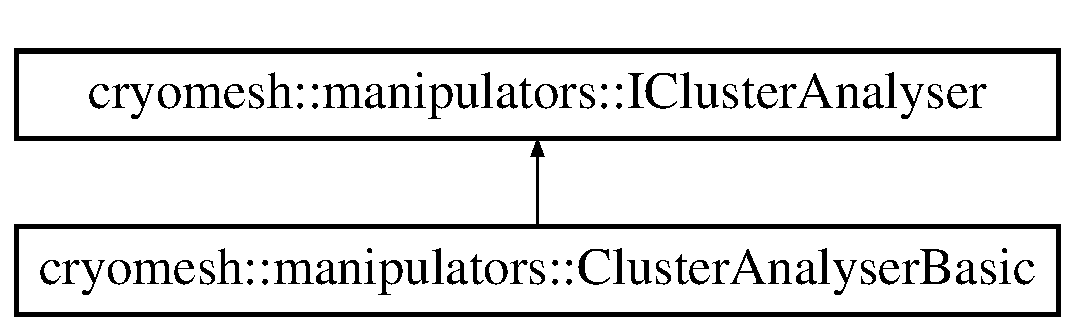
\includegraphics[height=2.000000cm]{classcryomesh_1_1manipulators_1_1IClusterAnalyser}
\end{center}
\end{figure}
\subsection*{\-Classes}
\begin{DoxyCompactItemize}
\item 
struct \hyperlink{structcryomesh_1_1manipulators_1_1IClusterAnalyser_1_1EnergyVariationWeightingMap}{\-Energy\-Variation\-Weighting\-Map}
\item 
struct \hyperlink{structcryomesh_1_1manipulators_1_1IClusterAnalyser_1_1RestructuringCountdown}{\-Restructuring\-Countdown}
\begin{DoxyCompactList}\small\item\em \-Class to hold together information on whether we can act to restructure items. \end{DoxyCompactList}\end{DoxyCompactItemize}
\subsection*{\-Public \-Types}
\begin{DoxyCompactItemize}
\item 
enum \hyperlink{classcryomesh_1_1manipulators_1_1IClusterAnalyser_a28a17f8e1363cfb575bacdf213b0781b}{\-Energy\-Variation} \{ \*
\hyperlink{classcryomesh_1_1manipulators_1_1IClusterAnalyser_a28a17f8e1363cfb575bacdf213b0781ba5b6d113aa10f4f70e703a35a39f828d6}{\-N\-O\-N\-E} =  2048, 
\hyperlink{classcryomesh_1_1manipulators_1_1IClusterAnalyser_a28a17f8e1363cfb575bacdf213b0781ba1378201d3fdbeeb653457ffb75488e85}{\-O\-U\-T\-\_\-\-O\-F\-\_\-\-R\-A\-N\-G\-E\-\_\-\-P\-O\-S\-I\-T\-I\-V\-E} =  1024, 
\hyperlink{classcryomesh_1_1manipulators_1_1IClusterAnalyser_a28a17f8e1363cfb575bacdf213b0781baef559139b3fe444fe2b3a24cd8ad0e4d}{\-H\-I\-G\-H\-\_\-\-P\-O\-S\-I\-T\-I\-V\-E} =  512, 
\hyperlink{classcryomesh_1_1manipulators_1_1IClusterAnalyser_a28a17f8e1363cfb575bacdf213b0781baab792b24800c050c84be43dddc08e75c}{\-M\-E\-D\-I\-U\-M\-\_\-\-P\-O\-S\-I\-T\-I\-V\-E} =  256, 
\*
\hyperlink{classcryomesh_1_1manipulators_1_1IClusterAnalyser_a28a17f8e1363cfb575bacdf213b0781ba7d05576fa354d351682eb4fa4f7261e8}{\-S\-M\-A\-L\-L\-\_\-\-P\-O\-S\-I\-T\-I\-V\-E} =  128, 
\hyperlink{classcryomesh_1_1manipulators_1_1IClusterAnalyser_a28a17f8e1363cfb575bacdf213b0781ba27c546877668dfb253e99b8985e4785e}{\-S\-T\-A\-G\-N\-A\-N\-T\-\_\-\-P\-O\-S\-I\-T\-I\-V\-E} =  64, 
\hyperlink{classcryomesh_1_1manipulators_1_1IClusterAnalyser_a28a17f8e1363cfb575bacdf213b0781bae3634dc08cf07554af474b718a1e6b1a}{\-Z\-E\-R\-O} =  32, 
\hyperlink{classcryomesh_1_1manipulators_1_1IClusterAnalyser_a28a17f8e1363cfb575bacdf213b0781bae2174fd5cb8c0db340ffd78804b56947}{\-S\-T\-A\-G\-N\-A\-N\-T\-\_\-\-N\-E\-G\-A\-T\-I\-V\-E} =  16, 
\*
\hyperlink{classcryomesh_1_1manipulators_1_1IClusterAnalyser_a28a17f8e1363cfb575bacdf213b0781bafab77593c2979a49443331f74ed2ba3b}{\-S\-M\-A\-L\-L\-\_\-\-N\-E\-G\-A\-T\-I\-V\-E} =  8, 
\hyperlink{classcryomesh_1_1manipulators_1_1IClusterAnalyser_a28a17f8e1363cfb575bacdf213b0781ba745d3d50f982c9db34f6b55d589ab24c}{\-M\-E\-D\-I\-U\-M\-\_\-\-N\-E\-G\-A\-T\-I\-V\-E} =  4, 
\hyperlink{classcryomesh_1_1manipulators_1_1IClusterAnalyser_a28a17f8e1363cfb575bacdf213b0781bac5cc71ffb113077fb2d67cafb98210e0}{\-H\-I\-G\-H\-\_\-\-N\-E\-G\-A\-T\-I\-V\-E} =  2, 
\hyperlink{classcryomesh_1_1manipulators_1_1IClusterAnalyser_a28a17f8e1363cfb575bacdf213b0781ba531a3f899bfdad545563f019093505c8}{\-O\-U\-T\-\_\-\-O\-F\-\_\-\-R\-A\-N\-G\-E\-\_\-\-N\-E\-G\-A\-T\-I\-V\-E} =  1
 \}
\end{DoxyCompactItemize}
\subsection*{\-Public \-Member \-Functions}
\begin{DoxyCompactItemize}
\item 
\hyperlink{classcryomesh_1_1manipulators_1_1IClusterAnalyser_aa3b46d3be5c9ab4eeaccd95316412b6a}{\-I\-Cluster\-Analyser} ()
\item 
virtual \hyperlink{classcryomesh_1_1manipulators_1_1IClusterAnalyser_af75850be2d49a54411cf5c9274c1ec76}{$\sim$\-I\-Cluster\-Analyser} ()
\item 
virtual \hyperlink{classcryomesh_1_1manipulators_1_1ClusterAnalysisData}{\-Cluster\-Analysis\-Data} \hyperlink{classcryomesh_1_1manipulators_1_1IClusterAnalyser_a0b8594c4b41ed14d5a94d191d1ab11fd}{analyse\-Cluster} (const \hyperlink{classcryomesh_1_1structures_1_1Cluster}{structures\-::\-Cluster} \&cluster, const std\-::map$<$ int, std\-::list$<$ \hyperlink{classcryomesh_1_1manipulators_1_1ClusterAnalysisData}{\-Cluster\-Analysis\-Data} $>$ $>$ \&histories)=0
\begin{DoxyCompactList}\small\item\em \-Run an analysis on the cluster to decide what action to take on nodes and connections. \end{DoxyCompactList}\item 
virtual \hyperlink{classcryomesh_1_1manipulators_1_1ClusterAnalysisData}{\-Cluster\-Analysis\-Data} \hyperlink{classcryomesh_1_1manipulators_1_1IClusterAnalyser_a1f666c2ccf0a6564510c8b4f062e2e21}{calculate\-Range\-Energies} (const std\-::list$<$ \hyperlink{classcryomesh_1_1manipulators_1_1ClusterAnalysisData}{\-Cluster\-Analysis\-Data} $>$ \&history) const =0
\begin{DoxyCompactList}\small\item\em \-Calculate the range energies stats. \end{DoxyCompactList}\item 
virtual \hyperlink{structcryomesh_1_1manipulators_1_1IClusterAnalyser_1_1EnergyVariationWeightingMap}{\-Energy\-Variation\-Weighting\-Map} \hyperlink{classcryomesh_1_1manipulators_1_1IClusterAnalyser_a27db139b4aa43f0c008de165d2f22f5b}{get\-Energy\-Variation\-Map} (const double energy\-\_\-input, double range) const =0
\item 
const \hyperlink{structcryomesh_1_1manipulators_1_1IClusterAnalyser_1_1RestructuringCountdown}{\-Restructuring\-Countdown} \& \hyperlink{classcryomesh_1_1manipulators_1_1IClusterAnalyser_af8eb711949e1d69bbe31b564ff9ab340}{get\-Connection\-Restructuring} () const 
\item 
const \hyperlink{structcryomesh_1_1manipulators_1_1IClusterAnalyser_1_1RestructuringCountdown}{\-Restructuring\-Countdown} \& \hyperlink{classcryomesh_1_1manipulators_1_1IClusterAnalyser_a72da7d8f63441671b8ebd1f4cd994347}{get\-Node\-Restructuring} () const 
\end{DoxyCompactItemize}
\subsection*{\-Protected \-Attributes}
\begin{DoxyCompactItemize}
\item 
\hyperlink{structcryomesh_1_1manipulators_1_1IClusterAnalyser_1_1RestructuringCountdown}{\-Restructuring\-Countdown} \hyperlink{classcryomesh_1_1manipulators_1_1IClusterAnalyser_a78d90b9829e4188ded3d94da49c6887a}{node\-Restructuring}
\item 
\hyperlink{structcryomesh_1_1manipulators_1_1IClusterAnalyser_1_1RestructuringCountdown}{\-Restructuring\-Countdown} \hyperlink{classcryomesh_1_1manipulators_1_1IClusterAnalyser_ae0442c245ec17e22d51ffd05c3a2f86e}{connection\-Restructuring}
\end{DoxyCompactItemize}


\subsection{\-Detailed \-Description}


\-Definition at line 17 of file \-I\-Cluster\-Analyser.\-h.



\subsection{\-Member \-Enumeration \-Documentation}
\hypertarget{classcryomesh_1_1manipulators_1_1IClusterAnalyser_a28a17f8e1363cfb575bacdf213b0781b}{\index{cryomesh\-::manipulators\-::\-I\-Cluster\-Analyser@{cryomesh\-::manipulators\-::\-I\-Cluster\-Analyser}!\-Energy\-Variation@{\-Energy\-Variation}}
\index{\-Energy\-Variation@{\-Energy\-Variation}!cryomesh::manipulators::IClusterAnalyser@{cryomesh\-::manipulators\-::\-I\-Cluster\-Analyser}}
\subsubsection[{\-Energy\-Variation}]{\setlength{\rightskip}{0pt plus 5cm}enum {\bf cryomesh\-::manipulators\-::\-I\-Cluster\-Analyser\-::\-Energy\-Variation}}}\label{classcryomesh_1_1manipulators_1_1IClusterAnalyser_a28a17f8e1363cfb575bacdf213b0781b}
\begin{Desc}
\item[\-Enumerator\-: ]\par
\begin{description}
\index{\-N\-O\-N\-E@{\-N\-O\-N\-E}!cryomesh\-::manipulators\-::\-I\-Cluster\-Analyser@{cryomesh\-::manipulators\-::\-I\-Cluster\-Analyser}}\index{cryomesh\-::manipulators\-::\-I\-Cluster\-Analyser@{cryomesh\-::manipulators\-::\-I\-Cluster\-Analyser}!\-N\-O\-N\-E@{\-N\-O\-N\-E}}\item[{\em 
\hypertarget{classcryomesh_1_1manipulators_1_1IClusterAnalyser_a28a17f8e1363cfb575bacdf213b0781ba5b6d113aa10f4f70e703a35a39f828d6}{\-N\-O\-N\-E}\label{classcryomesh_1_1manipulators_1_1IClusterAnalyser_a28a17f8e1363cfb575bacdf213b0781ba5b6d113aa10f4f70e703a35a39f828d6}
}]\index{\-O\-U\-T\-\_\-\-O\-F\-\_\-\-R\-A\-N\-G\-E\-\_\-\-P\-O\-S\-I\-T\-I\-V\-E@{\-O\-U\-T\-\_\-\-O\-F\-\_\-\-R\-A\-N\-G\-E\-\_\-\-P\-O\-S\-I\-T\-I\-V\-E}!cryomesh\-::manipulators\-::\-I\-Cluster\-Analyser@{cryomesh\-::manipulators\-::\-I\-Cluster\-Analyser}}\index{cryomesh\-::manipulators\-::\-I\-Cluster\-Analyser@{cryomesh\-::manipulators\-::\-I\-Cluster\-Analyser}!\-O\-U\-T\-\_\-\-O\-F\-\_\-\-R\-A\-N\-G\-E\-\_\-\-P\-O\-S\-I\-T\-I\-V\-E@{\-O\-U\-T\-\_\-\-O\-F\-\_\-\-R\-A\-N\-G\-E\-\_\-\-P\-O\-S\-I\-T\-I\-V\-E}}\item[{\em 
\hypertarget{classcryomesh_1_1manipulators_1_1IClusterAnalyser_a28a17f8e1363cfb575bacdf213b0781ba1378201d3fdbeeb653457ffb75488e85}{\-O\-U\-T\-\_\-\-O\-F\-\_\-\-R\-A\-N\-G\-E\-\_\-\-P\-O\-S\-I\-T\-I\-V\-E}\label{classcryomesh_1_1manipulators_1_1IClusterAnalyser_a28a17f8e1363cfb575bacdf213b0781ba1378201d3fdbeeb653457ffb75488e85}
}]\index{\-H\-I\-G\-H\-\_\-\-P\-O\-S\-I\-T\-I\-V\-E@{\-H\-I\-G\-H\-\_\-\-P\-O\-S\-I\-T\-I\-V\-E}!cryomesh\-::manipulators\-::\-I\-Cluster\-Analyser@{cryomesh\-::manipulators\-::\-I\-Cluster\-Analyser}}\index{cryomesh\-::manipulators\-::\-I\-Cluster\-Analyser@{cryomesh\-::manipulators\-::\-I\-Cluster\-Analyser}!\-H\-I\-G\-H\-\_\-\-P\-O\-S\-I\-T\-I\-V\-E@{\-H\-I\-G\-H\-\_\-\-P\-O\-S\-I\-T\-I\-V\-E}}\item[{\em 
\hypertarget{classcryomesh_1_1manipulators_1_1IClusterAnalyser_a28a17f8e1363cfb575bacdf213b0781baef559139b3fe444fe2b3a24cd8ad0e4d}{\-H\-I\-G\-H\-\_\-\-P\-O\-S\-I\-T\-I\-V\-E}\label{classcryomesh_1_1manipulators_1_1IClusterAnalyser_a28a17f8e1363cfb575bacdf213b0781baef559139b3fe444fe2b3a24cd8ad0e4d}
}]\index{\-M\-E\-D\-I\-U\-M\-\_\-\-P\-O\-S\-I\-T\-I\-V\-E@{\-M\-E\-D\-I\-U\-M\-\_\-\-P\-O\-S\-I\-T\-I\-V\-E}!cryomesh\-::manipulators\-::\-I\-Cluster\-Analyser@{cryomesh\-::manipulators\-::\-I\-Cluster\-Analyser}}\index{cryomesh\-::manipulators\-::\-I\-Cluster\-Analyser@{cryomesh\-::manipulators\-::\-I\-Cluster\-Analyser}!\-M\-E\-D\-I\-U\-M\-\_\-\-P\-O\-S\-I\-T\-I\-V\-E@{\-M\-E\-D\-I\-U\-M\-\_\-\-P\-O\-S\-I\-T\-I\-V\-E}}\item[{\em 
\hypertarget{classcryomesh_1_1manipulators_1_1IClusterAnalyser_a28a17f8e1363cfb575bacdf213b0781baab792b24800c050c84be43dddc08e75c}{\-M\-E\-D\-I\-U\-M\-\_\-\-P\-O\-S\-I\-T\-I\-V\-E}\label{classcryomesh_1_1manipulators_1_1IClusterAnalyser_a28a17f8e1363cfb575bacdf213b0781baab792b24800c050c84be43dddc08e75c}
}]\index{\-S\-M\-A\-L\-L\-\_\-\-P\-O\-S\-I\-T\-I\-V\-E@{\-S\-M\-A\-L\-L\-\_\-\-P\-O\-S\-I\-T\-I\-V\-E}!cryomesh\-::manipulators\-::\-I\-Cluster\-Analyser@{cryomesh\-::manipulators\-::\-I\-Cluster\-Analyser}}\index{cryomesh\-::manipulators\-::\-I\-Cluster\-Analyser@{cryomesh\-::manipulators\-::\-I\-Cluster\-Analyser}!\-S\-M\-A\-L\-L\-\_\-\-P\-O\-S\-I\-T\-I\-V\-E@{\-S\-M\-A\-L\-L\-\_\-\-P\-O\-S\-I\-T\-I\-V\-E}}\item[{\em 
\hypertarget{classcryomesh_1_1manipulators_1_1IClusterAnalyser_a28a17f8e1363cfb575bacdf213b0781ba7d05576fa354d351682eb4fa4f7261e8}{\-S\-M\-A\-L\-L\-\_\-\-P\-O\-S\-I\-T\-I\-V\-E}\label{classcryomesh_1_1manipulators_1_1IClusterAnalyser_a28a17f8e1363cfb575bacdf213b0781ba7d05576fa354d351682eb4fa4f7261e8}
}]\index{\-S\-T\-A\-G\-N\-A\-N\-T\-\_\-\-P\-O\-S\-I\-T\-I\-V\-E@{\-S\-T\-A\-G\-N\-A\-N\-T\-\_\-\-P\-O\-S\-I\-T\-I\-V\-E}!cryomesh\-::manipulators\-::\-I\-Cluster\-Analyser@{cryomesh\-::manipulators\-::\-I\-Cluster\-Analyser}}\index{cryomesh\-::manipulators\-::\-I\-Cluster\-Analyser@{cryomesh\-::manipulators\-::\-I\-Cluster\-Analyser}!\-S\-T\-A\-G\-N\-A\-N\-T\-\_\-\-P\-O\-S\-I\-T\-I\-V\-E@{\-S\-T\-A\-G\-N\-A\-N\-T\-\_\-\-P\-O\-S\-I\-T\-I\-V\-E}}\item[{\em 
\hypertarget{classcryomesh_1_1manipulators_1_1IClusterAnalyser_a28a17f8e1363cfb575bacdf213b0781ba27c546877668dfb253e99b8985e4785e}{\-S\-T\-A\-G\-N\-A\-N\-T\-\_\-\-P\-O\-S\-I\-T\-I\-V\-E}\label{classcryomesh_1_1manipulators_1_1IClusterAnalyser_a28a17f8e1363cfb575bacdf213b0781ba27c546877668dfb253e99b8985e4785e}
}]\index{\-Z\-E\-R\-O@{\-Z\-E\-R\-O}!cryomesh\-::manipulators\-::\-I\-Cluster\-Analyser@{cryomesh\-::manipulators\-::\-I\-Cluster\-Analyser}}\index{cryomesh\-::manipulators\-::\-I\-Cluster\-Analyser@{cryomesh\-::manipulators\-::\-I\-Cluster\-Analyser}!\-Z\-E\-R\-O@{\-Z\-E\-R\-O}}\item[{\em 
\hypertarget{classcryomesh_1_1manipulators_1_1IClusterAnalyser_a28a17f8e1363cfb575bacdf213b0781bae3634dc08cf07554af474b718a1e6b1a}{\-Z\-E\-R\-O}\label{classcryomesh_1_1manipulators_1_1IClusterAnalyser_a28a17f8e1363cfb575bacdf213b0781bae3634dc08cf07554af474b718a1e6b1a}
}]\index{\-S\-T\-A\-G\-N\-A\-N\-T\-\_\-\-N\-E\-G\-A\-T\-I\-V\-E@{\-S\-T\-A\-G\-N\-A\-N\-T\-\_\-\-N\-E\-G\-A\-T\-I\-V\-E}!cryomesh\-::manipulators\-::\-I\-Cluster\-Analyser@{cryomesh\-::manipulators\-::\-I\-Cluster\-Analyser}}\index{cryomesh\-::manipulators\-::\-I\-Cluster\-Analyser@{cryomesh\-::manipulators\-::\-I\-Cluster\-Analyser}!\-S\-T\-A\-G\-N\-A\-N\-T\-\_\-\-N\-E\-G\-A\-T\-I\-V\-E@{\-S\-T\-A\-G\-N\-A\-N\-T\-\_\-\-N\-E\-G\-A\-T\-I\-V\-E}}\item[{\em 
\hypertarget{classcryomesh_1_1manipulators_1_1IClusterAnalyser_a28a17f8e1363cfb575bacdf213b0781bae2174fd5cb8c0db340ffd78804b56947}{\-S\-T\-A\-G\-N\-A\-N\-T\-\_\-\-N\-E\-G\-A\-T\-I\-V\-E}\label{classcryomesh_1_1manipulators_1_1IClusterAnalyser_a28a17f8e1363cfb575bacdf213b0781bae2174fd5cb8c0db340ffd78804b56947}
}]\index{\-S\-M\-A\-L\-L\-\_\-\-N\-E\-G\-A\-T\-I\-V\-E@{\-S\-M\-A\-L\-L\-\_\-\-N\-E\-G\-A\-T\-I\-V\-E}!cryomesh\-::manipulators\-::\-I\-Cluster\-Analyser@{cryomesh\-::manipulators\-::\-I\-Cluster\-Analyser}}\index{cryomesh\-::manipulators\-::\-I\-Cluster\-Analyser@{cryomesh\-::manipulators\-::\-I\-Cluster\-Analyser}!\-S\-M\-A\-L\-L\-\_\-\-N\-E\-G\-A\-T\-I\-V\-E@{\-S\-M\-A\-L\-L\-\_\-\-N\-E\-G\-A\-T\-I\-V\-E}}\item[{\em 
\hypertarget{classcryomesh_1_1manipulators_1_1IClusterAnalyser_a28a17f8e1363cfb575bacdf213b0781bafab77593c2979a49443331f74ed2ba3b}{\-S\-M\-A\-L\-L\-\_\-\-N\-E\-G\-A\-T\-I\-V\-E}\label{classcryomesh_1_1manipulators_1_1IClusterAnalyser_a28a17f8e1363cfb575bacdf213b0781bafab77593c2979a49443331f74ed2ba3b}
}]\index{\-M\-E\-D\-I\-U\-M\-\_\-\-N\-E\-G\-A\-T\-I\-V\-E@{\-M\-E\-D\-I\-U\-M\-\_\-\-N\-E\-G\-A\-T\-I\-V\-E}!cryomesh\-::manipulators\-::\-I\-Cluster\-Analyser@{cryomesh\-::manipulators\-::\-I\-Cluster\-Analyser}}\index{cryomesh\-::manipulators\-::\-I\-Cluster\-Analyser@{cryomesh\-::manipulators\-::\-I\-Cluster\-Analyser}!\-M\-E\-D\-I\-U\-M\-\_\-\-N\-E\-G\-A\-T\-I\-V\-E@{\-M\-E\-D\-I\-U\-M\-\_\-\-N\-E\-G\-A\-T\-I\-V\-E}}\item[{\em 
\hypertarget{classcryomesh_1_1manipulators_1_1IClusterAnalyser_a28a17f8e1363cfb575bacdf213b0781ba745d3d50f982c9db34f6b55d589ab24c}{\-M\-E\-D\-I\-U\-M\-\_\-\-N\-E\-G\-A\-T\-I\-V\-E}\label{classcryomesh_1_1manipulators_1_1IClusterAnalyser_a28a17f8e1363cfb575bacdf213b0781ba745d3d50f982c9db34f6b55d589ab24c}
}]\index{\-H\-I\-G\-H\-\_\-\-N\-E\-G\-A\-T\-I\-V\-E@{\-H\-I\-G\-H\-\_\-\-N\-E\-G\-A\-T\-I\-V\-E}!cryomesh\-::manipulators\-::\-I\-Cluster\-Analyser@{cryomesh\-::manipulators\-::\-I\-Cluster\-Analyser}}\index{cryomesh\-::manipulators\-::\-I\-Cluster\-Analyser@{cryomesh\-::manipulators\-::\-I\-Cluster\-Analyser}!\-H\-I\-G\-H\-\_\-\-N\-E\-G\-A\-T\-I\-V\-E@{\-H\-I\-G\-H\-\_\-\-N\-E\-G\-A\-T\-I\-V\-E}}\item[{\em 
\hypertarget{classcryomesh_1_1manipulators_1_1IClusterAnalyser_a28a17f8e1363cfb575bacdf213b0781bac5cc71ffb113077fb2d67cafb98210e0}{\-H\-I\-G\-H\-\_\-\-N\-E\-G\-A\-T\-I\-V\-E}\label{classcryomesh_1_1manipulators_1_1IClusterAnalyser_a28a17f8e1363cfb575bacdf213b0781bac5cc71ffb113077fb2d67cafb98210e0}
}]\index{\-O\-U\-T\-\_\-\-O\-F\-\_\-\-R\-A\-N\-G\-E\-\_\-\-N\-E\-G\-A\-T\-I\-V\-E@{\-O\-U\-T\-\_\-\-O\-F\-\_\-\-R\-A\-N\-G\-E\-\_\-\-N\-E\-G\-A\-T\-I\-V\-E}!cryomesh\-::manipulators\-::\-I\-Cluster\-Analyser@{cryomesh\-::manipulators\-::\-I\-Cluster\-Analyser}}\index{cryomesh\-::manipulators\-::\-I\-Cluster\-Analyser@{cryomesh\-::manipulators\-::\-I\-Cluster\-Analyser}!\-O\-U\-T\-\_\-\-O\-F\-\_\-\-R\-A\-N\-G\-E\-\_\-\-N\-E\-G\-A\-T\-I\-V\-E@{\-O\-U\-T\-\_\-\-O\-F\-\_\-\-R\-A\-N\-G\-E\-\_\-\-N\-E\-G\-A\-T\-I\-V\-E}}\item[{\em 
\hypertarget{classcryomesh_1_1manipulators_1_1IClusterAnalyser_a28a17f8e1363cfb575bacdf213b0781ba531a3f899bfdad545563f019093505c8}{\-O\-U\-T\-\_\-\-O\-F\-\_\-\-R\-A\-N\-G\-E\-\_\-\-N\-E\-G\-A\-T\-I\-V\-E}\label{classcryomesh_1_1manipulators_1_1IClusterAnalyser_a28a17f8e1363cfb575bacdf213b0781ba531a3f899bfdad545563f019093505c8}
}]\end{description}
\end{Desc}



\-Definition at line 136 of file \-I\-Cluster\-Analyser.\-h.



\subsection{\-Constructor \& \-Destructor \-Documentation}
\hypertarget{classcryomesh_1_1manipulators_1_1IClusterAnalyser_aa3b46d3be5c9ab4eeaccd95316412b6a}{\index{cryomesh\-::manipulators\-::\-I\-Cluster\-Analyser@{cryomesh\-::manipulators\-::\-I\-Cluster\-Analyser}!\-I\-Cluster\-Analyser@{\-I\-Cluster\-Analyser}}
\index{\-I\-Cluster\-Analyser@{\-I\-Cluster\-Analyser}!cryomesh::manipulators::IClusterAnalyser@{cryomesh\-::manipulators\-::\-I\-Cluster\-Analyser}}
\subsubsection[{\-I\-Cluster\-Analyser}]{\setlength{\rightskip}{0pt plus 5cm}{\bf cryomesh\-::manipulators\-::\-I\-Cluster\-Analyser\-::\-I\-Cluster\-Analyser} (
\begin{DoxyParamCaption}
{}
\end{DoxyParamCaption}
)\hspace{0.3cm}{\ttfamily  \mbox{[}inline\mbox{]}}}}\label{classcryomesh_1_1manipulators_1_1IClusterAnalyser_aa3b46d3be5c9ab4eeaccd95316412b6a}


\-Definition at line 168 of file \-I\-Cluster\-Analyser.\-h.

\hypertarget{classcryomesh_1_1manipulators_1_1IClusterAnalyser_af75850be2d49a54411cf5c9274c1ec76}{\index{cryomesh\-::manipulators\-::\-I\-Cluster\-Analyser@{cryomesh\-::manipulators\-::\-I\-Cluster\-Analyser}!$\sim$\-I\-Cluster\-Analyser@{$\sim$\-I\-Cluster\-Analyser}}
\index{$\sim$\-I\-Cluster\-Analyser@{$\sim$\-I\-Cluster\-Analyser}!cryomesh::manipulators::IClusterAnalyser@{cryomesh\-::manipulators\-::\-I\-Cluster\-Analyser}}
\subsubsection[{$\sim$\-I\-Cluster\-Analyser}]{\setlength{\rightskip}{0pt plus 5cm}virtual {\bf cryomesh\-::manipulators\-::\-I\-Cluster\-Analyser\-::$\sim$\-I\-Cluster\-Analyser} (
\begin{DoxyParamCaption}
{}
\end{DoxyParamCaption}
)\hspace{0.3cm}{\ttfamily  \mbox{[}inline, virtual\mbox{]}}}}\label{classcryomesh_1_1manipulators_1_1IClusterAnalyser_af75850be2d49a54411cf5c9274c1ec76}


\-Definition at line 171 of file \-I\-Cluster\-Analyser.\-h.



\subsection{\-Member \-Function \-Documentation}
\hypertarget{classcryomesh_1_1manipulators_1_1IClusterAnalyser_a0b8594c4b41ed14d5a94d191d1ab11fd}{\index{cryomesh\-::manipulators\-::\-I\-Cluster\-Analyser@{cryomesh\-::manipulators\-::\-I\-Cluster\-Analyser}!analyse\-Cluster@{analyse\-Cluster}}
\index{analyse\-Cluster@{analyse\-Cluster}!cryomesh::manipulators::IClusterAnalyser@{cryomesh\-::manipulators\-::\-I\-Cluster\-Analyser}}
\subsubsection[{analyse\-Cluster}]{\setlength{\rightskip}{0pt plus 5cm}virtual {\bf \-Cluster\-Analysis\-Data} {\bf cryomesh\-::manipulators\-::\-I\-Cluster\-Analyser\-::analyse\-Cluster} (
\begin{DoxyParamCaption}
\item[{const {\bf structures\-::\-Cluster} \&}]{cluster, }
\item[{const std\-::map$<$ int, std\-::list$<$ {\bf \-Cluster\-Analysis\-Data} $>$ $>$ \&}]{histories}
\end{DoxyParamCaption}
)\hspace{0.3cm}{\ttfamily  \mbox{[}pure virtual\mbox{]}}}}\label{classcryomesh_1_1manipulators_1_1IClusterAnalyser_a0b8594c4b41ed14d5a94d191d1ab11fd}


\-Run an analysis on the cluster to decide what action to take on nodes and connections. 


\begin{DoxyParams}{\-Parameters}
{\em const} & \hyperlink{classcryomesh_1_1structures_1_1Cluster}{structures\-::\-Cluster} \& \-The cluster to analyse \\
\hline
{\em const} & std\-::list$<$\-Cluster\-Analysis\-Data$>$ \-The historical analysis data to use\\
\hline
\end{DoxyParams}
\begin{DoxyReturn}{\-Returns}
\hyperlink{classcryomesh_1_1manipulators_1_1ClusterAnalysisData}{\-Cluster\-Analysis\-Data} \-The reulting analytical data 
\end{DoxyReturn}


\-Implemented in \hyperlink{classcryomesh_1_1manipulators_1_1ClusterAnalyserBasic_ad98be2e316548236479ce5da459d530b}{cryomesh\-::manipulators\-::\-Cluster\-Analyser\-Basic}.

\hypertarget{classcryomesh_1_1manipulators_1_1IClusterAnalyser_a1f666c2ccf0a6564510c8b4f062e2e21}{\index{cryomesh\-::manipulators\-::\-I\-Cluster\-Analyser@{cryomesh\-::manipulators\-::\-I\-Cluster\-Analyser}!calculate\-Range\-Energies@{calculate\-Range\-Energies}}
\index{calculate\-Range\-Energies@{calculate\-Range\-Energies}!cryomesh::manipulators::IClusterAnalyser@{cryomesh\-::manipulators\-::\-I\-Cluster\-Analyser}}
\subsubsection[{calculate\-Range\-Energies}]{\setlength{\rightskip}{0pt plus 5cm}virtual {\bf \-Cluster\-Analysis\-Data} {\bf cryomesh\-::manipulators\-::\-I\-Cluster\-Analyser\-::calculate\-Range\-Energies} (
\begin{DoxyParamCaption}
\item[{const std\-::list$<$ {\bf \-Cluster\-Analysis\-Data} $>$ \&}]{history}
\end{DoxyParamCaption}
) const\hspace{0.3cm}{\ttfamily  \mbox{[}pure virtual\mbox{]}}}}\label{classcryomesh_1_1manipulators_1_1IClusterAnalyser_a1f666c2ccf0a6564510c8b4f062e2e21}


\-Calculate the range energies stats. 


\begin{DoxyParams}{\-Parameters}
{\em const} & std\-::list$<$\-Cluster\-Analysis\-Data$>$ \& \-The history range to work with\\
\hline
\end{DoxyParams}
\begin{DoxyReturn}{\-Returns}
\hyperlink{classcryomesh_1_1manipulators_1_1ClusterAnalysisData}{\-Cluster\-Analysis\-Data} \-The resulting cluster analysis data 
\end{DoxyReturn}


\-Implemented in \hyperlink{classcryomesh_1_1manipulators_1_1ClusterAnalyserBasic_ab4e344d193d764d0e60aaed87c9770b3}{cryomesh\-::manipulators\-::\-Cluster\-Analyser\-Basic}.

\hypertarget{classcryomesh_1_1manipulators_1_1IClusterAnalyser_af8eb711949e1d69bbe31b564ff9ab340}{\index{cryomesh\-::manipulators\-::\-I\-Cluster\-Analyser@{cryomesh\-::manipulators\-::\-I\-Cluster\-Analyser}!get\-Connection\-Restructuring@{get\-Connection\-Restructuring}}
\index{get\-Connection\-Restructuring@{get\-Connection\-Restructuring}!cryomesh::manipulators::IClusterAnalyser@{cryomesh\-::manipulators\-::\-I\-Cluster\-Analyser}}
\subsubsection[{get\-Connection\-Restructuring}]{\setlength{\rightskip}{0pt plus 5cm}const {\bf \-Restructuring\-Countdown}\& {\bf cryomesh\-::manipulators\-::\-I\-Cluster\-Analyser\-::get\-Connection\-Restructuring} (
\begin{DoxyParamCaption}
{}
\end{DoxyParamCaption}
) const\hspace{0.3cm}{\ttfamily  \mbox{[}inline\mbox{]}}}}\label{classcryomesh_1_1manipulators_1_1IClusterAnalyser_af8eb711949e1d69bbe31b564ff9ab340}


\-Definition at line 198 of file \-I\-Cluster\-Analyser.\-h.



\-References connection\-Restructuring.

\hypertarget{classcryomesh_1_1manipulators_1_1IClusterAnalyser_a27db139b4aa43f0c008de165d2f22f5b}{\index{cryomesh\-::manipulators\-::\-I\-Cluster\-Analyser@{cryomesh\-::manipulators\-::\-I\-Cluster\-Analyser}!get\-Energy\-Variation\-Map@{get\-Energy\-Variation\-Map}}
\index{get\-Energy\-Variation\-Map@{get\-Energy\-Variation\-Map}!cryomesh::manipulators::IClusterAnalyser@{cryomesh\-::manipulators\-::\-I\-Cluster\-Analyser}}
\subsubsection[{get\-Energy\-Variation\-Map}]{\setlength{\rightskip}{0pt plus 5cm}virtual {\bf \-Energy\-Variation\-Weighting\-Map} {\bf cryomesh\-::manipulators\-::\-I\-Cluster\-Analyser\-::get\-Energy\-Variation\-Map} (
\begin{DoxyParamCaption}
\item[{const double}]{energy\-\_\-input, }
\item[{double}]{range}
\end{DoxyParamCaption}
) const\hspace{0.3cm}{\ttfamily  \mbox{[}pure virtual\mbox{]}}}}\label{classcryomesh_1_1manipulators_1_1IClusterAnalyser_a27db139b4aa43f0c008de165d2f22f5b}


\-Implemented in \hyperlink{classcryomesh_1_1manipulators_1_1ClusterAnalyserBasic_a8870233415221b9c971a30452fb9452a}{cryomesh\-::manipulators\-::\-Cluster\-Analyser\-Basic}.

\hypertarget{classcryomesh_1_1manipulators_1_1IClusterAnalyser_a72da7d8f63441671b8ebd1f4cd994347}{\index{cryomesh\-::manipulators\-::\-I\-Cluster\-Analyser@{cryomesh\-::manipulators\-::\-I\-Cluster\-Analyser}!get\-Node\-Restructuring@{get\-Node\-Restructuring}}
\index{get\-Node\-Restructuring@{get\-Node\-Restructuring}!cryomesh::manipulators::IClusterAnalyser@{cryomesh\-::manipulators\-::\-I\-Cluster\-Analyser}}
\subsubsection[{get\-Node\-Restructuring}]{\setlength{\rightskip}{0pt plus 5cm}const {\bf \-Restructuring\-Countdown}\& {\bf cryomesh\-::manipulators\-::\-I\-Cluster\-Analyser\-::get\-Node\-Restructuring} (
\begin{DoxyParamCaption}
{}
\end{DoxyParamCaption}
) const\hspace{0.3cm}{\ttfamily  \mbox{[}inline\mbox{]}}}}\label{classcryomesh_1_1manipulators_1_1IClusterAnalyser_a72da7d8f63441671b8ebd1f4cd994347}


\-Definition at line 201 of file \-I\-Cluster\-Analyser.\-h.



\-References node\-Restructuring.



\subsection{\-Member \-Data \-Documentation}
\hypertarget{classcryomesh_1_1manipulators_1_1IClusterAnalyser_ae0442c245ec17e22d51ffd05c3a2f86e}{\index{cryomesh\-::manipulators\-::\-I\-Cluster\-Analyser@{cryomesh\-::manipulators\-::\-I\-Cluster\-Analyser}!connection\-Restructuring@{connection\-Restructuring}}
\index{connection\-Restructuring@{connection\-Restructuring}!cryomesh::manipulators::IClusterAnalyser@{cryomesh\-::manipulators\-::\-I\-Cluster\-Analyser}}
\subsubsection[{connection\-Restructuring}]{\setlength{\rightskip}{0pt plus 5cm}{\bf \-Restructuring\-Countdown} {\bf cryomesh\-::manipulators\-::\-I\-Cluster\-Analyser\-::connection\-Restructuring}\hspace{0.3cm}{\ttfamily  \mbox{[}protected\mbox{]}}}}\label{classcryomesh_1_1manipulators_1_1IClusterAnalyser_ae0442c245ec17e22d51ffd05c3a2f86e}


\-Definition at line 206 of file \-I\-Cluster\-Analyser.\-h.



\-Referenced by cryomesh\-::manipulators\-::\-Cluster\-Analyser\-Basic\-::analyse\-Cluster(), and get\-Connection\-Restructuring().

\hypertarget{classcryomesh_1_1manipulators_1_1IClusterAnalyser_a78d90b9829e4188ded3d94da49c6887a}{\index{cryomesh\-::manipulators\-::\-I\-Cluster\-Analyser@{cryomesh\-::manipulators\-::\-I\-Cluster\-Analyser}!node\-Restructuring@{node\-Restructuring}}
\index{node\-Restructuring@{node\-Restructuring}!cryomesh::manipulators::IClusterAnalyser@{cryomesh\-::manipulators\-::\-I\-Cluster\-Analyser}}
\subsubsection[{node\-Restructuring}]{\setlength{\rightskip}{0pt plus 5cm}{\bf \-Restructuring\-Countdown} {\bf cryomesh\-::manipulators\-::\-I\-Cluster\-Analyser\-::node\-Restructuring}\hspace{0.3cm}{\ttfamily  \mbox{[}protected\mbox{]}}}}\label{classcryomesh_1_1manipulators_1_1IClusterAnalyser_a78d90b9829e4188ded3d94da49c6887a}


\-Definition at line 205 of file \-I\-Cluster\-Analyser.\-h.



\-Referenced by cryomesh\-::manipulators\-::\-Cluster\-Analyser\-Basic\-::analyse\-Cluster(), and get\-Node\-Restructuring().



\-The documentation for this class was generated from the following file\-:\begin{DoxyCompactItemize}
\item 
/home/niall/\-Projects/\-Eclipse/\-C\-P\-P/cryomesh/src/manipulators/\hyperlink{IClusterAnalyser_8h}{\-I\-Cluster\-Analyser.\-h}\end{DoxyCompactItemize}

\hypertarget{classcryomesh_1_1components_1_1Impulse}{\section{cryomesh\-:\-:components\-:\-:\-Impulse \-Class \-Reference}
\label{classcryomesh_1_1components_1_1Impulse}\index{cryomesh\-::components\-::\-Impulse@{cryomesh\-::components\-::\-Impulse}}
}


\hyperlink{classcryomesh_1_1components_1_1Impulse}{\-Impulse} is a mobile information packet to be passed between \-Nodes.  




{\ttfamily \#include $<$\-Impulse.\-h$>$}

\subsection*{\-Public \-Member \-Functions}
\begin{DoxyCompactItemize}
\item 
\hyperlink{classcryomesh_1_1components_1_1Impulse_aff44f52a706b48a74fc34b3dc2e26d38}{\-Impulse} ()
\begin{DoxyCompactList}\small\item\em \-Constructor. \end{DoxyCompactList}\item 
\hyperlink{classcryomesh_1_1components_1_1Impulse_afd7597df2534ba3d0b7d91d3c0b64a55}{\-Impulse} (const double max\-\_\-y, const int length, const int delay=0)
\begin{DoxyCompactList}\small\item\em \-Construct a from a curve with max f(x) and length and set starting cycle to start\-Cycle, which defaults to the present, 'now' cycle. \end{DoxyCompactList}\item 
\hyperlink{classcryomesh_1_1components_1_1Impulse_a61915a9d92e7c7601be4a005794c0c89}{\-Impulse} (const double max\-\_\-y, const int length, const int delay, boost\-::shared\-\_\-ptr$<$ \hyperlink{classcryomesh_1_1components_1_1ActivityTimerDistance}{\-Activity\-Timer\-Distance} $>$)
\begin{DoxyCompactList}\small\item\em \-Construct a from a curve with max f(x) and length and set starting cycle to start\-Cycle, and an activity timer. \end{DoxyCompactList}\item 
\hyperlink{classcryomesh_1_1components_1_1Impulse_af9ec60048bf54aaf5ee3e93dd4b87f3d}{\-Impulse} (const \hyperlink{classcryomesh_1_1components_1_1Impulse}{\-Impulse} \&obj)
\item 
virtual \hyperlink{classcryomesh_1_1components_1_1Impulse_a3801df3c6dba70d0467f070fa346efa5}{$\sim$\-Impulse} ()
\begin{DoxyCompactList}\small\item\em \-Destructor. \end{DoxyCompactList}\item 
void \hyperlink{classcryomesh_1_1components_1_1Impulse_a5da6ee1f9d1be136d23c36c377258a4d}{randomise} (double positive\-\_\-bias=0.\-5)
\item 
bool \hyperlink{classcryomesh_1_1components_1_1Impulse_a9c87bdf033d68e93204704078860aef6}{is\-Active} () const 
\begin{DoxyCompactList}\small\item\em \-Is the \hyperlink{classcryomesh_1_1components_1_1Impulse}{\-Impulse} active on current cycle. \end{DoxyCompactList}\item 
bool \hyperlink{classcryomesh_1_1components_1_1Impulse_a69f3c99fcbcaa31682ed42085608e476}{is\-Active} (const \hyperlink{classcryomesh_1_1common_1_1Cycle}{common\-::\-Cycle} \&cycle) const 
\begin{DoxyCompactList}\small\item\em \-Is the \hyperlink{classcryomesh_1_1components_1_1Impulse}{\-Impulse} active on cycle. \end{DoxyCompactList}\item 
bool \hyperlink{classcryomesh_1_1components_1_1Impulse_a07543fdf1e3eb3e2cb8196259fae480a}{is\-Active} (const \hyperlink{classcryomesh_1_1common_1_1Cycle}{common\-::\-Cycle} \&start\-Cycle, const \hyperlink{classcryomesh_1_1common_1_1Cycle}{common\-::\-Cycle} \&end\-Cycle) const 
\begin{DoxyCompactList}\small\item\em \-Is the \hyperlink{classcryomesh_1_1components_1_1Impulse}{\-Impulse} active at some point in cycle range. \end{DoxyCompactList}\item 
double \hyperlink{classcryomesh_1_1components_1_1Impulse_a50ff12cf26ce360c37ec6ed93aad2ea5}{get\-Activity} (\hyperlink{classcryomesh_1_1common_1_1Cycle}{common\-::\-Cycle} cycle) const 
\begin{DoxyCompactList}\small\item\em \-Get activity at cycle. \end{DoxyCompactList}\item 
double \hyperlink{classcryomesh_1_1components_1_1Impulse_a73cb97b2371198e44f726de54c9c36fa}{get\-Activity} () const 
\begin{DoxyCompactList}\small\item\em \-Get activity at current cycle. \end{DoxyCompactList}\item 
double \hyperlink{classcryomesh_1_1components_1_1Impulse_a9607961d67264b1431bc6f0871ab71e0}{get\-Activity\-Maximum} () const 
\begin{DoxyCompactList}\small\item\em \-Get maximum activity. \end{DoxyCompactList}\item 
double \hyperlink{classcryomesh_1_1components_1_1Impulse_a9ccf24929b1d73630bd02ead060a5b15}{get\-Activity\-Minimum} () const 
\begin{DoxyCompactList}\small\item\em \-Get minimum activity. \end{DoxyCompactList}\item 
virtual \hyperlink{classcryomesh_1_1components_1_1Impulse}{\-Impulse} \& \hyperlink{classcryomesh_1_1components_1_1Impulse_a21d17ce78d670cfc7082d5d09767c359}{invert} ()
\begin{DoxyCompactList}\small\item\em \-Invert the impulse. \end{DoxyCompactList}\item 
\hyperlink{classcryomesh_1_1common_1_1Cycle}{common\-::\-Cycle} \hyperlink{classcryomesh_1_1components_1_1Impulse_a348598ef30bd651b94ebbc0cdc46cb28}{get\-First\-Active\-Cycle} () const 
\begin{DoxyCompactList}\small\item\em \-Get the first active cycle. \end{DoxyCompactList}\item 
void \hyperlink{classcryomesh_1_1components_1_1Impulse_abe6cffbd621e68849bff60ce6799ff4b}{set\-First\-Active\-Cycle} (const \hyperlink{classcryomesh_1_1common_1_1Cycle}{common\-::\-Cycle} cycle)
\begin{DoxyCompactList}\small\item\em \-Set the first active cycle. \end{DoxyCompactList}\item 
\hyperlink{classcryomesh_1_1common_1_1Cycle}{common\-::\-Cycle} \hyperlink{classcryomesh_1_1components_1_1Impulse_ac91dae86e992103f921da77f0cfe0d02}{get\-Last\-Active\-Cycle} () const 
\begin{DoxyCompactList}\small\item\em \-Get the last active cycle. \end{DoxyCompactList}\item 
const std\-::list$<$ double $>$ \& \hyperlink{classcryomesh_1_1components_1_1Impulse_a959076c6c59932abeaa73ca6de2e4167}{get\-Activities} () const 
\begin{DoxyCompactList}\small\item\em \-Get activities. \end{DoxyCompactList}\item 
const boost\-::shared\-\_\-ptr\*
$<$ \hyperlink{classcryomesh_1_1components_1_1ActivityTimerDistance}{\-Activity\-Timer\-Distance} $>$ \hyperlink{classcryomesh_1_1components_1_1Impulse_a356adeb4cebeb35ecef7231718fb20cd}{get\-Activity\-Timer} () const 
\begin{DoxyCompactList}\small\item\em \-Get activity timer. \end{DoxyCompactList}\item 
boost\-::shared\-\_\-ptr\*
$<$ \hyperlink{classcryomesh_1_1components_1_1ActivityTimerDistance}{\-Activity\-Timer\-Distance} $>$ \hyperlink{classcryomesh_1_1components_1_1Impulse_aac5460017f7adceba53aea31b1bc5bfe}{get\-Mutable\-Activity\-Timer} ()
\begin{DoxyCompactList}\small\item\em \-Get mutable activity timer. \end{DoxyCompactList}\item 
void \hyperlink{classcryomesh_1_1components_1_1Impulse_a04ecc67f3bf21f922c29d9e8afd3d04d}{set\-Activity\-Timer} (boost\-::shared\-\_\-ptr$<$ \hyperlink{classcryomesh_1_1components_1_1ActivityTimerDistance}{\-Activity\-Timer\-Distance} $>$ timer)
\begin{DoxyCompactList}\small\item\em \-Set activity timer. \end{DoxyCompactList}\item 
int \hyperlink{classcryomesh_1_1components_1_1Impulse_a6d0fd21f516b5182dd357b59f2112c64}{get\-Activity\-Delay} () const 
\item 
void \hyperlink{classcryomesh_1_1components_1_1Impulse_a800479ed06132eb56d0bc15c8aa40d8a}{set\-Activity\-Delay} (int delay)
\item 
const \hyperlink{classcryomesh_1_1components_1_1Impulse}{\-Impulse} \hyperlink{classcryomesh_1_1components_1_1Impulse_aca088f62a2bf95978952633e530e601c}{operator+} (const \hyperlink{classcryomesh_1_1components_1_1Impulse}{\-Impulse} \&obj) const 
\begin{DoxyCompactList}\small\item\em \-Non-\/destructive addition operator. \end{DoxyCompactList}\item 
\hyperlink{classcryomesh_1_1components_1_1Impulse}{\-Impulse} \& \hyperlink{classcryomesh_1_1components_1_1Impulse_a6f5351eea5c38586fe5bb3092b3626af}{operator+=} (const \hyperlink{classcryomesh_1_1components_1_1Impulse}{\-Impulse} \&obj)
\begin{DoxyCompactList}\small\item\em \-Destructive addition and assignment operator. \end{DoxyCompactList}\item 
\hyperlink{classcryomesh_1_1components_1_1Impulse}{\-Impulse} \& \hyperlink{classcryomesh_1_1components_1_1Impulse_a77e225470110ea77db3969cbaa2e276a}{operator=} (const \hyperlink{classcryomesh_1_1components_1_1Impulse}{\-Impulse} \&obj)
\begin{DoxyCompactList}\small\item\em \-Assignment operator. \end{DoxyCompactList}\item 
bool \hyperlink{classcryomesh_1_1components_1_1Impulse_a8351a5a0e6afc72fa26ab306226ccab0}{operator==} (const \hyperlink{classcryomesh_1_1components_1_1Impulse}{\-Impulse} \&obj) const 
\begin{DoxyCompactList}\small\item\em \-Comparator operator. \end{DoxyCompactList}\item 
bool \hyperlink{classcryomesh_1_1components_1_1Impulse_ac26da063e408d5493cd33f2014dfa875}{operator!=} (const \hyperlink{classcryomesh_1_1components_1_1Impulse}{\-Impulse} \&obj) const 
\begin{DoxyCompactList}\small\item\em \-Not comparator operator. \end{DoxyCompactList}\item 
virtual void \hyperlink{classcryomesh_1_1components_1_1Impulse_ad3a3e47e23c5443a9df0df9c3c53a8ac}{enable\-Debug} (bool b)
\end{DoxyCompactItemize}
\subsection*{\-Static \-Public \-Member \-Functions}
\begin{DoxyCompactItemize}
\item 
static boost\-::shared\-\_\-ptr$<$ \hyperlink{classcryomesh_1_1components_1_1Impulse}{\-Impulse} $>$ \hyperlink{classcryomesh_1_1components_1_1Impulse_ae88e7ff0cacf1ca6f323f66c97819c7a}{get\-Trigger\-Impulse} ()
\begin{DoxyCompactList}\small\item\em \-Get a 'trigger' impulse, a maximum impulse. \end{DoxyCompactList}\item 
static boost\-::shared\-\_\-ptr$<$ \hyperlink{classcryomesh_1_1components_1_1Impulse}{\-Impulse} $>$ \hyperlink{classcryomesh_1_1components_1_1Impulse_a9433c8dbc841beb6e3bfa63dd99ed838}{get\-Random} (double positive\-\_\-bias=0.\-5)
\begin{DoxyCompactList}\small\item\em \-Get a randomised impulse. \end{DoxyCompactList}\end{DoxyCompactItemize}
\subsection*{\-Static \-Public \-Attributes}
\begin{DoxyCompactItemize}
\item 
static const double \hyperlink{classcryomesh_1_1components_1_1Impulse_aa581812f8f38b8a08d6f9ec9d301c455}{\-F\-O\-R\-C\-E\-D\-\_\-\-T\-R\-I\-G\-G\-E\-R\-\_\-\-A\-C\-T\-I\-V\-I\-T\-Y} = 1000
\item 
static const double \hyperlink{classcryomesh_1_1components_1_1Impulse_af8e9eb795f1ea3cef81d6afeb7166ad2}{\-M\-A\-X\-\_\-\-A\-C\-T\-I\-V\-I\-T\-Y} = 1
\item 
static const double \hyperlink{classcryomesh_1_1components_1_1Impulse_a3cc162bae9213a65a6aa241b256e1a84}{\-M\-I\-N\-\_\-\-A\-C\-T\-I\-V\-I\-T\-Y} = -\/1
\item 
static const int \hyperlink{classcryomesh_1_1components_1_1Impulse_a449f5f6a08af50b2e66703931ef3cd6c}{\-M\-A\-X\-\_\-\-A\-C\-T\-I\-V\-I\-T\-Y\-\_\-\-L\-E\-N\-G\-T\-H} = 20
\item 
static const int \hyperlink{classcryomesh_1_1components_1_1Impulse_ac24594fb7419a2f3e9f4d753dfae562f}{\-M\-I\-N\-\_\-\-A\-C\-T\-I\-V\-I\-T\-Y\-\_\-\-L\-E\-N\-G\-T\-H} = 1
\item 
static const double \hyperlink{classcryomesh_1_1components_1_1Impulse_a831758cc2e20d4a2d10b71f8c7698fd1}{\-M\-I\-N\-\_\-\-A\-C\-T\-I\-V\-I\-T\-Y\-\_\-\-M\-A\-G\-N\-I\-T\-U\-D\-E} = 0.\-01
\item 
static const int \hyperlink{classcryomesh_1_1components_1_1Impulse_a7537a73569989ce84f0ab1b10e07ee94}{\-M\-I\-N\-\_\-\-A\-C\-T\-I\-V\-I\-T\-Y\-\_\-\-D\-E\-L\-A\-Y} = 0
\item 
static const int \hyperlink{classcryomesh_1_1components_1_1Impulse_afc1ae22e801a9dbf9bbb170d97d3411b}{\-M\-A\-X\-\_\-\-A\-C\-T\-I\-V\-I\-T\-Y\-\_\-\-D\-E\-L\-A\-Y} = 10
\end{DoxyCompactItemize}
\subsection*{\-Protected \-Member \-Functions}
\begin{DoxyCompactItemize}
\item 
double \hyperlink{classcryomesh_1_1components_1_1Impulse_a4bdb9cdab1998c670d3e7f46190fa45d}{get\-Activity\-Boundary} (bool maximal) const 
\begin{DoxyCompactList}\small\item\em \-Get the boundary value of activity. \end{DoxyCompactList}\end{DoxyCompactItemize}
\subsection*{\-Private \-Attributes}
\begin{DoxyCompactItemize}
\item 
\hyperlink{classcryomesh_1_1common_1_1Cycle}{common\-::\-Cycle} \hyperlink{classcryomesh_1_1components_1_1Impulse_a1e60e9449535dde78c2a342b873022f7}{first\-Active\-Cycle}
\begin{DoxyCompactList}\small\item\em \-The first cycle that this \hyperlink{classcryomesh_1_1components_1_1Impulse}{\-Impulse} has activity. \end{DoxyCompactList}\item 
\hyperlink{classcryomesh_1_1common_1_1Cycle}{common\-::\-Cycle} \hyperlink{classcryomesh_1_1components_1_1Impulse_adc17d78b2127229c3acdaefb7b697f7e}{last\-Active\-Cycle}
\begin{DoxyCompactList}\small\item\em \-The lase cycle that this \hyperlink{classcryomesh_1_1components_1_1Impulse}{\-Impulse} has activity. \end{DoxyCompactList}\item 
int \hyperlink{classcryomesh_1_1components_1_1Impulse_ae491ccf924dc04674fb604a5258e0580}{activity\-Delay}
\item 
boost\-::shared\-\_\-ptr\*
$<$ \hyperlink{classcryomesh_1_1components_1_1ActivityTimerDistance}{\-Activity\-Timer\-Distance} $>$ \hyperlink{classcryomesh_1_1components_1_1Impulse_a6fc33296a0683cc08c5ea7404632a793}{activity\-Timer}
\end{DoxyCompactItemize}
\subsection*{\-Friends}
\begin{DoxyCompactItemize}
\item 
std\-::ostream \& \hyperlink{classcryomesh_1_1components_1_1Impulse_ab7b2621039dab2cd363725afdf5d667a}{operator$<$$<$} (std\-::ostream \&os, const \hyperlink{classcryomesh_1_1components_1_1Impulse}{\-Impulse} \&obj)
\begin{DoxyCompactList}\small\item\em \-To stream operator. \end{DoxyCompactList}\end{DoxyCompactItemize}


\subsection{\-Detailed \-Description}
\hyperlink{classcryomesh_1_1components_1_1Impulse}{\-Impulse} is a mobile information packet to be passed between \-Nodes. 

\-Impulses represent information generated by a \hyperlink{classcryomesh_1_1components_1_1Node}{\-Node} firing \-They are propagated along a connection \-Can be modified by the overlying \-Mesh as they propagate 

\-Definition at line 31 of file \-Impulse.\-h.



\subsection{\-Constructor \& \-Destructor \-Documentation}
\hypertarget{classcryomesh_1_1components_1_1Impulse_aff44f52a706b48a74fc34b3dc2e26d38}{\index{cryomesh\-::components\-::\-Impulse@{cryomesh\-::components\-::\-Impulse}!\-Impulse@{\-Impulse}}
\index{\-Impulse@{\-Impulse}!cryomesh::components::Impulse@{cryomesh\-::components\-::\-Impulse}}
\subsubsection[{\-Impulse}]{\setlength{\rightskip}{0pt plus 5cm}{\bf cryomesh\-::components\-::\-Impulse\-::\-Impulse} (
\begin{DoxyParamCaption}
{}
\end{DoxyParamCaption}
)}}\label{classcryomesh_1_1components_1_1Impulse_aff44f52a706b48a74fc34b3dc2e26d38}


\-Constructor. 

\-Constructor for \hyperlink{classcryomesh_1_1components_1_1Impulse}{\-Impulse}


\begin{DoxyParams}{\-Parameters}
{\em bool} & random \-If true then randomise the impulse on creation \\
\hline
\end{DoxyParams}


\-Definition at line 45 of file \-Impulse.\-cpp.



\-References \-M\-I\-N\-\_\-\-A\-C\-T\-I\-V\-I\-T\-Y\-\_\-\-L\-E\-N\-G\-T\-H, set\-Activity\-Timer(), and set\-First\-Active\-Cycle().

\hypertarget{classcryomesh_1_1components_1_1Impulse_afd7597df2534ba3d0b7d91d3c0b64a55}{\index{cryomesh\-::components\-::\-Impulse@{cryomesh\-::components\-::\-Impulse}!\-Impulse@{\-Impulse}}
\index{\-Impulse@{\-Impulse}!cryomesh::components::Impulse@{cryomesh\-::components\-::\-Impulse}}
\subsubsection[{\-Impulse}]{\setlength{\rightskip}{0pt plus 5cm}{\bf cryomesh\-::components\-::\-Impulse\-::\-Impulse} (
\begin{DoxyParamCaption}
\item[{const double}]{max\-\_\-y, }
\item[{const int}]{length, }
\item[{const int}]{delay = {\ttfamily 0}}
\end{DoxyParamCaption}
)}}\label{classcryomesh_1_1components_1_1Impulse_afd7597df2534ba3d0b7d91d3c0b64a55}


\-Construct a from a curve with max f(x) and length and set starting cycle to start\-Cycle, which defaults to the present, 'now' cycle. 


\begin{DoxyParams}{\-Parameters}
{\em const} & int max\-\_\-y \-Boundary value of curve \\
\hline
{\em const} & int length \-Length of \hyperlink{classcryomesh_1_1components_1_1Impulse}{\-Impulse} \\
\hline
{\em int} & \-Delay before starting impulse \\
\hline
\end{DoxyParams}


\-Definition at line 54 of file \-Impulse.\-cpp.



\-References \-M\-I\-N\-\_\-\-A\-C\-T\-I\-V\-I\-T\-Y\-\_\-\-L\-E\-N\-G\-T\-H, set\-Activity\-Delay(), set\-Activity\-Timer(), and set\-First\-Active\-Cycle().

\hypertarget{classcryomesh_1_1components_1_1Impulse_a61915a9d92e7c7601be4a005794c0c89}{\index{cryomesh\-::components\-::\-Impulse@{cryomesh\-::components\-::\-Impulse}!\-Impulse@{\-Impulse}}
\index{\-Impulse@{\-Impulse}!cryomesh::components::Impulse@{cryomesh\-::components\-::\-Impulse}}
\subsubsection[{\-Impulse}]{\setlength{\rightskip}{0pt plus 5cm}{\bf cryomesh\-::components\-::\-Impulse\-::\-Impulse} (
\begin{DoxyParamCaption}
\item[{const double}]{max\-\_\-y, }
\item[{const int}]{length, }
\item[{const int}]{delay, }
\item[{boost\-::shared\-\_\-ptr$<$ {\bf \-Activity\-Timer\-Distance} $>$}]{timer}
\end{DoxyParamCaption}
)}}\label{classcryomesh_1_1components_1_1Impulse_a61915a9d92e7c7601be4a005794c0c89}


\-Construct a from a curve with max f(x) and length and set starting cycle to start\-Cycle, and an activity timer. 


\begin{DoxyParams}{\-Parameters}
{\em const} & int max\-\_\-y \-Boundary value of curve \\
\hline
{\em const} & int length \-Length of \hyperlink{classcryomesh_1_1components_1_1Impulse}{\-Impulse} \\
\hline
{\em int} & \-Delay before starting impulse \\
\hline
{\em boost\-::shared\-\_\-ptr$<$\-Activity\-Timer$>$} & timer \-The activity timer associated with this \\
\hline
\end{DoxyParams}


\-Definition at line 65 of file \-Impulse.\-cpp.



\-References \-M\-I\-N\-\_\-\-A\-C\-T\-I\-V\-I\-T\-Y\-\_\-\-L\-E\-N\-G\-T\-H, set\-Activity\-Delay(), set\-Activity\-Timer(), and set\-First\-Active\-Cycle().

\hypertarget{classcryomesh_1_1components_1_1Impulse_af9ec60048bf54aaf5ee3e93dd4b87f3d}{\index{cryomesh\-::components\-::\-Impulse@{cryomesh\-::components\-::\-Impulse}!\-Impulse@{\-Impulse}}
\index{\-Impulse@{\-Impulse}!cryomesh::components::Impulse@{cryomesh\-::components\-::\-Impulse}}
\subsubsection[{\-Impulse}]{\setlength{\rightskip}{0pt plus 5cm}{\bf cryomesh\-::components\-::\-Impulse\-::\-Impulse} (
\begin{DoxyParamCaption}
\item[{const {\bf \-Impulse} \&}]{obj}
\end{DoxyParamCaption}
)}}\label{classcryomesh_1_1components_1_1Impulse_af9ec60048bf54aaf5ee3e93dd4b87f3d}


\-Definition at line 75 of file \-Impulse.\-cpp.



\-References first\-Active\-Cycle, get\-Activity\-Delay(), get\-Activity\-Timer(), get\-First\-Active\-Cycle(), get\-Last\-Active\-Cycle(), last\-Active\-Cycle, set\-Activity\-Delay(), and set\-Activity\-Timer().

\hypertarget{classcryomesh_1_1components_1_1Impulse_a3801df3c6dba70d0467f070fa346efa5}{\index{cryomesh\-::components\-::\-Impulse@{cryomesh\-::components\-::\-Impulse}!$\sim$\-Impulse@{$\sim$\-Impulse}}
\index{$\sim$\-Impulse@{$\sim$\-Impulse}!cryomesh::components::Impulse@{cryomesh\-::components\-::\-Impulse}}
\subsubsection[{$\sim$\-Impulse}]{\setlength{\rightskip}{0pt plus 5cm}{\bf cryomesh\-::components\-::\-Impulse\-::$\sim$\-Impulse} (
\begin{DoxyParamCaption}
{}
\end{DoxyParamCaption}
)\hspace{0.3cm}{\ttfamily  \mbox{[}virtual\mbox{]}}}}\label{classcryomesh_1_1components_1_1Impulse_a3801df3c6dba70d0467f070fa346efa5}


\-Destructor. 

\-Destructor for \hyperlink{classcryomesh_1_1components_1_1Impulse}{\-Impulse} 

\-Definition at line 83 of file \-Impulse.\-cpp.



\subsection{\-Member \-Function \-Documentation}
\hypertarget{classcryomesh_1_1components_1_1Impulse_ad3a3e47e23c5443a9df0df9c3c53a8ac}{\index{cryomesh\-::components\-::\-Impulse@{cryomesh\-::components\-::\-Impulse}!enable\-Debug@{enable\-Debug}}
\index{enable\-Debug@{enable\-Debug}!cryomesh::components::Impulse@{cryomesh\-::components\-::\-Impulse}}
\subsubsection[{enable\-Debug}]{\setlength{\rightskip}{0pt plus 5cm}void {\bf cryomesh\-::components\-::\-Impulse\-::enable\-Debug} (
\begin{DoxyParamCaption}
\item[{bool}]{b}
\end{DoxyParamCaption}
)\hspace{0.3cm}{\ttfamily  \mbox{[}virtual\mbox{]}}}}\label{classcryomesh_1_1components_1_1Impulse_ad3a3e47e23c5443a9df0df9c3c53a8ac}


\-Definition at line 336 of file \-Impulse.\-cpp.

\hypertarget{classcryomesh_1_1components_1_1Impulse_a959076c6c59932abeaa73ca6de2e4167}{\index{cryomesh\-::components\-::\-Impulse@{cryomesh\-::components\-::\-Impulse}!get\-Activities@{get\-Activities}}
\index{get\-Activities@{get\-Activities}!cryomesh::components::Impulse@{cryomesh\-::components\-::\-Impulse}}
\subsubsection[{get\-Activities}]{\setlength{\rightskip}{0pt plus 5cm}const std\-::list$<$ double $>$ \& {\bf cryomesh\-::components\-::\-Impulse\-::get\-Activities} (
\begin{DoxyParamCaption}
{}
\end{DoxyParamCaption}
) const}}\label{classcryomesh_1_1components_1_1Impulse_a959076c6c59932abeaa73ca6de2e4167}


\-Get activities. 

\begin{DoxyReturn}{\-Returns}
const std\-::list$<$double$>$ \& \-The activities list 
\end{DoxyReturn}


\-Definition at line 192 of file \-Impulse.\-cpp.

\hypertarget{classcryomesh_1_1components_1_1Impulse_a50ff12cf26ce360c37ec6ed93aad2ea5}{\index{cryomesh\-::components\-::\-Impulse@{cryomesh\-::components\-::\-Impulse}!get\-Activity@{get\-Activity}}
\index{get\-Activity@{get\-Activity}!cryomesh::components::Impulse@{cryomesh\-::components\-::\-Impulse}}
\subsubsection[{get\-Activity}]{\setlength{\rightskip}{0pt plus 5cm}double {\bf cryomesh\-::components\-::\-Impulse\-::get\-Activity} (
\begin{DoxyParamCaption}
\item[{{\bf common\-::\-Cycle}}]{cycle}
\end{DoxyParamCaption}
) const}}\label{classcryomesh_1_1components_1_1Impulse_a50ff12cf26ce360c37ec6ed93aad2ea5}


\-Get activity at cycle. 

\-Sum all the \-Impulses in the collection on specified cycle and return activity


\begin{DoxyParams}{\-Parameters}
{\em int} & cycle \-The cycle to calculate the activity on\\
\hline
\end{DoxyParams}
\begin{DoxyReturn}{\-Returns}
double \-The activity on specified cycle 
\end{DoxyReturn}


\-Definition at line 129 of file \-Impulse.\-cpp.



\-References first\-Active\-Cycle, get\-First\-Active\-Cycle(), get\-Last\-Active\-Cycle(), last\-Active\-Cycle, and cryomesh\-::common\-::\-Cycle\-::to\-L\-Int().

\hypertarget{classcryomesh_1_1components_1_1Impulse_a73cb97b2371198e44f726de54c9c36fa}{\index{cryomesh\-::components\-::\-Impulse@{cryomesh\-::components\-::\-Impulse}!get\-Activity@{get\-Activity}}
\index{get\-Activity@{get\-Activity}!cryomesh::components::Impulse@{cryomesh\-::components\-::\-Impulse}}
\subsubsection[{get\-Activity}]{\setlength{\rightskip}{0pt plus 5cm}double {\bf cryomesh\-::components\-::\-Impulse\-::get\-Activity} (
\begin{DoxyParamCaption}
{}
\end{DoxyParamCaption}
) const}}\label{classcryomesh_1_1components_1_1Impulse_a73cb97b2371198e44f726de54c9c36fa}


\-Get activity at current cycle. 

\-Sum all the \-Impulses in the collection on the current cycle and return activity

\begin{DoxyReturn}{\-Returns}
double \-The activity on specified cycle 
\end{DoxyReturn}


\-Definition at line 125 of file \-Impulse.\-cpp.



\-References cryomesh\-::common\-::\-Time\-Keeper\-::get\-Time\-Keeper().

\hypertarget{classcryomesh_1_1components_1_1Impulse_a4bdb9cdab1998c670d3e7f46190fa45d}{\index{cryomesh\-::components\-::\-Impulse@{cryomesh\-::components\-::\-Impulse}!get\-Activity\-Boundary@{get\-Activity\-Boundary}}
\index{get\-Activity\-Boundary@{get\-Activity\-Boundary}!cryomesh::components::Impulse@{cryomesh\-::components\-::\-Impulse}}
\subsubsection[{get\-Activity\-Boundary}]{\setlength{\rightskip}{0pt plus 5cm}double {\bf cryomesh\-::components\-::\-Impulse\-::get\-Activity\-Boundary} (
\begin{DoxyParamCaption}
\item[{bool}]{maximal}
\end{DoxyParamCaption}
) const\hspace{0.3cm}{\ttfamily  \mbox{[}protected\mbox{]}}}}\label{classcryomesh_1_1components_1_1Impulse_a4bdb9cdab1998c670d3e7f46190fa45d}


\-Get the boundary value of activity. 


\begin{DoxyParams}{\-Parameters}
{\em bool} & maximal \-True if maximal boundary, false if minimal\\
\hline
\end{DoxyParams}
\begin{DoxyReturn}{\-Returns}
double \-The boundary value of activity 
\end{DoxyReturn}
\hypertarget{classcryomesh_1_1components_1_1Impulse_a6d0fd21f516b5182dd357b59f2112c64}{\index{cryomesh\-::components\-::\-Impulse@{cryomesh\-::components\-::\-Impulse}!get\-Activity\-Delay@{get\-Activity\-Delay}}
\index{get\-Activity\-Delay@{get\-Activity\-Delay}!cryomesh::components::Impulse@{cryomesh\-::components\-::\-Impulse}}
\subsubsection[{get\-Activity\-Delay}]{\setlength{\rightskip}{0pt plus 5cm}int {\bf cryomesh\-::components\-::\-Impulse\-::get\-Activity\-Delay} (
\begin{DoxyParamCaption}
{}
\end{DoxyParamCaption}
) const}}\label{classcryomesh_1_1components_1_1Impulse_a6d0fd21f516b5182dd357b59f2112c64}


\-Definition at line 208 of file \-Impulse.\-cpp.



\-References activity\-Delay.



\-Referenced by \-Impulse(), cryomesh\-::components\-::operator$<$$<$(), operator=(), and set\-First\-Active\-Cycle().

\hypertarget{classcryomesh_1_1components_1_1Impulse_a9607961d67264b1431bc6f0871ab71e0}{\index{cryomesh\-::components\-::\-Impulse@{cryomesh\-::components\-::\-Impulse}!get\-Activity\-Maximum@{get\-Activity\-Maximum}}
\index{get\-Activity\-Maximum@{get\-Activity\-Maximum}!cryomesh::components::Impulse@{cryomesh\-::components\-::\-Impulse}}
\subsubsection[{get\-Activity\-Maximum}]{\setlength{\rightskip}{0pt plus 5cm}double {\bf cryomesh\-::components\-::\-Impulse\-::get\-Activity\-Maximum} (
\begin{DoxyParamCaption}
{}
\end{DoxyParamCaption}
) const}}\label{classcryomesh_1_1components_1_1Impulse_a9607961d67264b1431bc6f0871ab71e0}


\-Get maximum activity. 

\-Find the maximum activity between start and end cycles

\begin{DoxyReturn}{\-Returns}
double \-The maximum activity 
\end{DoxyReturn}


\-Definition at line 156 of file \-Impulse.\-cpp.

\hypertarget{classcryomesh_1_1components_1_1Impulse_a9ccf24929b1d73630bd02ead060a5b15}{\index{cryomesh\-::components\-::\-Impulse@{cryomesh\-::components\-::\-Impulse}!get\-Activity\-Minimum@{get\-Activity\-Minimum}}
\index{get\-Activity\-Minimum@{get\-Activity\-Minimum}!cryomesh::components::Impulse@{cryomesh\-::components\-::\-Impulse}}
\subsubsection[{get\-Activity\-Minimum}]{\setlength{\rightskip}{0pt plus 5cm}double {\bf cryomesh\-::components\-::\-Impulse\-::get\-Activity\-Minimum} (
\begin{DoxyParamCaption}
{}
\end{DoxyParamCaption}
) const}}\label{classcryomesh_1_1components_1_1Impulse_a9ccf24929b1d73630bd02ead060a5b15}


\-Get minimum activity. 

\-Find the minimum activity between start and end cycles

\begin{DoxyReturn}{\-Returns}
double \-The minimum activity 
\end{DoxyReturn}


\-Definition at line 160 of file \-Impulse.\-cpp.

\hypertarget{classcryomesh_1_1components_1_1Impulse_a356adeb4cebeb35ecef7231718fb20cd}{\index{cryomesh\-::components\-::\-Impulse@{cryomesh\-::components\-::\-Impulse}!get\-Activity\-Timer@{get\-Activity\-Timer}}
\index{get\-Activity\-Timer@{get\-Activity\-Timer}!cryomesh::components::Impulse@{cryomesh\-::components\-::\-Impulse}}
\subsubsection[{get\-Activity\-Timer}]{\setlength{\rightskip}{0pt plus 5cm}const boost\-::shared\-\_\-ptr$<$ {\bf \-Activity\-Timer\-Distance} $>$ {\bf cryomesh\-::components\-::\-Impulse\-::get\-Activity\-Timer} (
\begin{DoxyParamCaption}
{}
\end{DoxyParamCaption}
) const}}\label{classcryomesh_1_1components_1_1Impulse_a356adeb4cebeb35ecef7231718fb20cd}


\-Get activity timer. 

\begin{DoxyReturn}{\-Returns}
boost\-::shared\-\_\-ptr$<$ Activity\-Timer $>$ activity\-Timer; \-The activity timer 
\end{DoxyReturn}


\-Definition at line 196 of file \-Impulse.\-cpp.



\-References activity\-Timer.



\-Referenced by \-Impulse(), cryomesh\-::components\-::operator$<$$<$(), and operator=().

\hypertarget{classcryomesh_1_1components_1_1Impulse_a348598ef30bd651b94ebbc0cdc46cb28}{\index{cryomesh\-::components\-::\-Impulse@{cryomesh\-::components\-::\-Impulse}!get\-First\-Active\-Cycle@{get\-First\-Active\-Cycle}}
\index{get\-First\-Active\-Cycle@{get\-First\-Active\-Cycle}!cryomesh::components::Impulse@{cryomesh\-::components\-::\-Impulse}}
\subsubsection[{get\-First\-Active\-Cycle}]{\setlength{\rightskip}{0pt plus 5cm}{\bf \-Cycle} {\bf cryomesh\-::components\-::\-Impulse\-::get\-First\-Active\-Cycle} (
\begin{DoxyParamCaption}
{}
\end{DoxyParamCaption}
) const}}\label{classcryomesh_1_1components_1_1Impulse_a348598ef30bd651b94ebbc0cdc46cb28}


\-Get the first active cycle. 

\begin{DoxyReturn}{\-Returns}
\-Cycle \-The first active cycle 
\end{DoxyReturn}


\-Definition at line 169 of file \-Impulse.\-cpp.



\-References first\-Active\-Cycle.



\-Referenced by cryomesh\-::components\-::\-Impulse\-Collection\-::clear\-Active\-Impulses(), get\-Activity(), \-Impulse(), operator+=(), cryomesh\-::components\-::operator$<$$<$(), operator=(), and operator==().

\hypertarget{classcryomesh_1_1components_1_1Impulse_ac91dae86e992103f921da77f0cfe0d02}{\index{cryomesh\-::components\-::\-Impulse@{cryomesh\-::components\-::\-Impulse}!get\-Last\-Active\-Cycle@{get\-Last\-Active\-Cycle}}
\index{get\-Last\-Active\-Cycle@{get\-Last\-Active\-Cycle}!cryomesh::components::Impulse@{cryomesh\-::components\-::\-Impulse}}
\subsubsection[{get\-Last\-Active\-Cycle}]{\setlength{\rightskip}{0pt plus 5cm}{\bf \-Cycle} {\bf cryomesh\-::components\-::\-Impulse\-::get\-Last\-Active\-Cycle} (
\begin{DoxyParamCaption}
{}
\end{DoxyParamCaption}
) const}}\label{classcryomesh_1_1components_1_1Impulse_ac91dae86e992103f921da77f0cfe0d02}


\-Get the last active cycle. 

\begin{DoxyReturn}{\-Returns}
\-Cycle \-The last active cycle 
\end{DoxyReturn}


\-Definition at line 188 of file \-Impulse.\-cpp.



\-References last\-Active\-Cycle.



\-Referenced by cryomesh\-::components\-::\-Impulse\-Collection\-::clear\-Active\-Impulses(), get\-Activity(), \-Impulse(), operator+=(), cryomesh\-::components\-::operator$<$$<$(), operator=(), and operator==().

\hypertarget{classcryomesh_1_1components_1_1Impulse_aac5460017f7adceba53aea31b1bc5bfe}{\index{cryomesh\-::components\-::\-Impulse@{cryomesh\-::components\-::\-Impulse}!get\-Mutable\-Activity\-Timer@{get\-Mutable\-Activity\-Timer}}
\index{get\-Mutable\-Activity\-Timer@{get\-Mutable\-Activity\-Timer}!cryomesh::components::Impulse@{cryomesh\-::components\-::\-Impulse}}
\subsubsection[{get\-Mutable\-Activity\-Timer}]{\setlength{\rightskip}{0pt plus 5cm}boost\-::shared\-\_\-ptr$<$ {\bf \-Activity\-Timer\-Distance} $>$ {\bf cryomesh\-::components\-::\-Impulse\-::get\-Mutable\-Activity\-Timer} (
\begin{DoxyParamCaption}
{}
\end{DoxyParamCaption}
)}}\label{classcryomesh_1_1components_1_1Impulse_aac5460017f7adceba53aea31b1bc5bfe}


\-Get mutable activity timer. 

\begin{DoxyReturn}{\-Returns}
boost\-::shared\-\_\-ptr$<$ Activity\-Timer $>$ activity\-Timer; \-The activity timer 
\end{DoxyReturn}


\-Definition at line 200 of file \-Impulse.\-cpp.



\-References activity\-Timer.

\hypertarget{classcryomesh_1_1components_1_1Impulse_a9433c8dbc841beb6e3bfa63dd99ed838}{\index{cryomesh\-::components\-::\-Impulse@{cryomesh\-::components\-::\-Impulse}!get\-Random@{get\-Random}}
\index{get\-Random@{get\-Random}!cryomesh::components::Impulse@{cryomesh\-::components\-::\-Impulse}}
\subsubsection[{get\-Random}]{\setlength{\rightskip}{0pt plus 5cm}boost\-::shared\-\_\-ptr$<$ {\bf \-Impulse} $>$ {\bf cryomesh\-::components\-::\-Impulse\-::get\-Random} (
\begin{DoxyParamCaption}
\item[{double}]{positive\-\_\-bias = {\ttfamily 0.5}}
\end{DoxyParamCaption}
)\hspace{0.3cm}{\ttfamily  \mbox{[}static\mbox{]}}}}\label{classcryomesh_1_1components_1_1Impulse_a9433c8dbc841beb6e3bfa63dd99ed838}


\-Get a randomised impulse. 


\begin{DoxyParams}{\-Parameters}
{\em double} & the (0,1) bias of a positive impulse outcome, 0 negative, 1, positive\\
\hline
\end{DoxyParams}
\begin{DoxyReturn}{\-Returns}
boost\-::shared\-\_\-ptr$<$\-Impulse$>$ \-The randomised impulse 
\end{DoxyReturn}


\-Definition at line 38 of file \-Impulse.\-cpp.



\-Referenced by cryomesh\-::components\-::\-Node\-Map\-::add\-Random\-Impulses(), and randomise().

\hypertarget{classcryomesh_1_1components_1_1Impulse_ae88e7ff0cacf1ca6f323f66c97819c7a}{\index{cryomesh\-::components\-::\-Impulse@{cryomesh\-::components\-::\-Impulse}!get\-Trigger\-Impulse@{get\-Trigger\-Impulse}}
\index{get\-Trigger\-Impulse@{get\-Trigger\-Impulse}!cryomesh::components::Impulse@{cryomesh\-::components\-::\-Impulse}}
\subsubsection[{get\-Trigger\-Impulse}]{\setlength{\rightskip}{0pt plus 5cm}boost\-::shared\-\_\-ptr$<$ {\bf \-Impulse} $>$ {\bf cryomesh\-::components\-::\-Impulse\-::get\-Trigger\-Impulse} (
\begin{DoxyParamCaption}
{}
\end{DoxyParamCaption}
)\hspace{0.3cm}{\ttfamily  \mbox{[}static\mbox{]}}}}\label{classcryomesh_1_1components_1_1Impulse_ae88e7ff0cacf1ca6f323f66c97819c7a}


\-Get a 'trigger' impulse, a maximum impulse. 

\begin{DoxyReturn}{\-Returns}
boost\-::shared\-\_\-ptr$<$\-Impulse$>$ \-The trigger impulse 
\end{DoxyReturn}


\-Definition at line 33 of file \-Impulse.\-cpp.



\-Referenced by cryomesh\-::components\-::\-Node\-::force\-Fire(), and cryomesh\-::structures\-::\-Fibre\-::trigger().

\hypertarget{classcryomesh_1_1components_1_1Impulse_a21d17ce78d670cfc7082d5d09767c359}{\index{cryomesh\-::components\-::\-Impulse@{cryomesh\-::components\-::\-Impulse}!invert@{invert}}
\index{invert@{invert}!cryomesh::components::Impulse@{cryomesh\-::components\-::\-Impulse}}
\subsubsection[{invert}]{\setlength{\rightskip}{0pt plus 5cm}{\bf \-Impulse} \& {\bf cryomesh\-::components\-::\-Impulse\-::invert} (
\begin{DoxyParamCaption}
{}
\end{DoxyParamCaption}
)\hspace{0.3cm}{\ttfamily  \mbox{[}virtual\mbox{]}}}}\label{classcryomesh_1_1components_1_1Impulse_a21d17ce78d670cfc7082d5d09767c359}


\-Invert the impulse. 

@ return \hyperlink{classcryomesh_1_1components_1_1Impulse}{\-Impulse} \& \-This object inverted 

\-Definition at line 164 of file \-Impulse.\-cpp.

\hypertarget{classcryomesh_1_1components_1_1Impulse_a9c87bdf033d68e93204704078860aef6}{\index{cryomesh\-::components\-::\-Impulse@{cryomesh\-::components\-::\-Impulse}!is\-Active@{is\-Active}}
\index{is\-Active@{is\-Active}!cryomesh::components::Impulse@{cryomesh\-::components\-::\-Impulse}}
\subsubsection[{is\-Active}]{\setlength{\rightskip}{0pt plus 5cm}bool {\bf cryomesh\-::components\-::\-Impulse\-::is\-Active} (
\begin{DoxyParamCaption}
{}
\end{DoxyParamCaption}
) const}}\label{classcryomesh_1_1components_1_1Impulse_a9c87bdf033d68e93204704078860aef6}


\-Is the \hyperlink{classcryomesh_1_1components_1_1Impulse}{\-Impulse} active on current cycle. 

\begin{DoxyReturn}{\-Returns}
bool \-True if active, false otherwise 
\end{DoxyReturn}


\-Definition at line 108 of file \-Impulse.\-cpp.



\-References cryomesh\-::common\-::\-Time\-Keeper\-::get\-Time\-Keeper().



\-Referenced by cryomesh\-::components\-::\-Impulse\-Collection\-::clear\-Active\-Impulses(), and is\-Active().

\hypertarget{classcryomesh_1_1components_1_1Impulse_a69f3c99fcbcaa31682ed42085608e476}{\index{cryomesh\-::components\-::\-Impulse@{cryomesh\-::components\-::\-Impulse}!is\-Active@{is\-Active}}
\index{is\-Active@{is\-Active}!cryomesh::components::Impulse@{cryomesh\-::components\-::\-Impulse}}
\subsubsection[{is\-Active}]{\setlength{\rightskip}{0pt plus 5cm}bool {\bf cryomesh\-::components\-::\-Impulse\-::is\-Active} (
\begin{DoxyParamCaption}
\item[{const {\bf common\-::\-Cycle} \&}]{cycle}
\end{DoxyParamCaption}
) const}}\label{classcryomesh_1_1components_1_1Impulse_a69f3c99fcbcaa31682ed42085608e476}


\-Is the \hyperlink{classcryomesh_1_1components_1_1Impulse}{\-Impulse} active on cycle. 

\begin{DoxyReturn}{\-Returns}
bool \-True if active, false otherwise 
\end{DoxyReturn}


\-Definition at line 112 of file \-Impulse.\-cpp.



\-References is\-Active().

\hypertarget{classcryomesh_1_1components_1_1Impulse_a07543fdf1e3eb3e2cb8196259fae480a}{\index{cryomesh\-::components\-::\-Impulse@{cryomesh\-::components\-::\-Impulse}!is\-Active@{is\-Active}}
\index{is\-Active@{is\-Active}!cryomesh::components::Impulse@{cryomesh\-::components\-::\-Impulse}}
\subsubsection[{is\-Active}]{\setlength{\rightskip}{0pt plus 5cm}bool {\bf cryomesh\-::components\-::\-Impulse\-::is\-Active} (
\begin{DoxyParamCaption}
\item[{const {\bf common\-::\-Cycle} \&}]{start\-Cycle, }
\item[{const {\bf common\-::\-Cycle} \&}]{end\-Cycle}
\end{DoxyParamCaption}
) const}}\label{classcryomesh_1_1components_1_1Impulse_a07543fdf1e3eb3e2cb8196259fae480a}


\-Is the \hyperlink{classcryomesh_1_1components_1_1Impulse}{\-Impulse} active at some point in cycle range. 

\begin{DoxyReturn}{\-Returns}
bool \-True if active, false otherwise 
\end{DoxyReturn}


\-Definition at line 116 of file \-Impulse.\-cpp.



\-References first\-Active\-Cycle, and last\-Active\-Cycle.

\hypertarget{classcryomesh_1_1components_1_1Impulse_ac26da063e408d5493cd33f2014dfa875}{\index{cryomesh\-::components\-::\-Impulse@{cryomesh\-::components\-::\-Impulse}!operator!=@{operator!=}}
\index{operator!=@{operator!=}!cryomesh::components::Impulse@{cryomesh\-::components\-::\-Impulse}}
\subsubsection[{operator!=}]{\setlength{\rightskip}{0pt plus 5cm}bool cryomesh\-::components\-::\-Impulse\-::operator!= (
\begin{DoxyParamCaption}
\item[{const {\bf \-Impulse} \&}]{obj}
\end{DoxyParamCaption}
) const}}\label{classcryomesh_1_1components_1_1Impulse_ac26da063e408d5493cd33f2014dfa875}


\-Not comparator operator. 


\begin{DoxyParams}{\-Parameters}
{\em const} & \hyperlink{classcryomesh_1_1components_1_1Impulse}{\-Impulse} \& obj \-R\-H\-S object\\
\hline
\end{DoxyParams}
\begin{DoxyReturn}{\-Returns}
bool \-True if not equal, false otherwise 
\end{DoxyReturn}


\-Definition at line 333 of file \-Impulse.\-cpp.

\hypertarget{classcryomesh_1_1components_1_1Impulse_aca088f62a2bf95978952633e530e601c}{\index{cryomesh\-::components\-::\-Impulse@{cryomesh\-::components\-::\-Impulse}!operator+@{operator+}}
\index{operator+@{operator+}!cryomesh::components::Impulse@{cryomesh\-::components\-::\-Impulse}}
\subsubsection[{operator+}]{\setlength{\rightskip}{0pt plus 5cm}const {\bf \-Impulse} cryomesh\-::components\-::\-Impulse\-::operator+ (
\begin{DoxyParamCaption}
\item[{const {\bf \-Impulse} \&}]{obj}
\end{DoxyParamCaption}
) const}}\label{classcryomesh_1_1components_1_1Impulse_aca088f62a2bf95978952633e530e601c}


\-Non-\/destructive addition operator. 


\begin{DoxyParams}{\-Parameters}
{\em const} & \hyperlink{classcryomesh_1_1components_1_1Impulse}{\-Impulse} \& obj \-R\-H\-S addition\\
\hline
\end{DoxyParams}
\begin{DoxyReturn}{\-Returns}
\hyperlink{classcryomesh_1_1components_1_1Impulse}{\-Impulse} \-New object after addition 
\end{DoxyReturn}


\-Definition at line 215 of file \-Impulse.\-cpp.

\hypertarget{classcryomesh_1_1components_1_1Impulse_a6f5351eea5c38586fe5bb3092b3626af}{\index{cryomesh\-::components\-::\-Impulse@{cryomesh\-::components\-::\-Impulse}!operator+=@{operator+=}}
\index{operator+=@{operator+=}!cryomesh::components::Impulse@{cryomesh\-::components\-::\-Impulse}}
\subsubsection[{operator+=}]{\setlength{\rightskip}{0pt plus 5cm}{\bf \-Impulse} \& cryomesh\-::components\-::\-Impulse\-::operator+= (
\begin{DoxyParamCaption}
\item[{const {\bf \-Impulse} \&}]{obj}
\end{DoxyParamCaption}
)}}\label{classcryomesh_1_1components_1_1Impulse_a6f5351eea5c38586fe5bb3092b3626af}


\-Destructive addition and assignment operator. 


\begin{DoxyParams}{\-Parameters}
{\em const} & \hyperlink{classcryomesh_1_1components_1_1Impulse}{\-Impulse} \& obj \-R\-H\-S addition\\
\hline
\end{DoxyParams}
\begin{DoxyReturn}{\-Returns}
\hyperlink{classcryomesh_1_1components_1_1Impulse}{\-Impulse} \& \-This object after addition and assignment 
\end{DoxyReturn}


\-Definition at line 221 of file \-Impulse.\-cpp.



\-References get\-First\-Active\-Cycle(), get\-Last\-Active\-Cycle(), and set\-First\-Active\-Cycle().

\hypertarget{classcryomesh_1_1components_1_1Impulse_a77e225470110ea77db3969cbaa2e276a}{\index{cryomesh\-::components\-::\-Impulse@{cryomesh\-::components\-::\-Impulse}!operator=@{operator=}}
\index{operator=@{operator=}!cryomesh::components::Impulse@{cryomesh\-::components\-::\-Impulse}}
\subsubsection[{operator=}]{\setlength{\rightskip}{0pt plus 5cm}{\bf \-Impulse} \& cryomesh\-::components\-::\-Impulse\-::operator= (
\begin{DoxyParamCaption}
\item[{const {\bf \-Impulse} \&}]{obj}
\end{DoxyParamCaption}
)}}\label{classcryomesh_1_1components_1_1Impulse_a77e225470110ea77db3969cbaa2e276a}


\-Assignment operator. 


\begin{DoxyParams}{\-Parameters}
{\em const} & \hyperlink{classcryomesh_1_1components_1_1Impulse}{\-Impulse} \& obj \-R\-H\-S assignment\\
\hline
\end{DoxyParams}
\begin{DoxyReturn}{\-Returns}
\hyperlink{classcryomesh_1_1components_1_1Impulse}{\-Impulse} \& \-This object after assignment 
\end{DoxyReturn}


\-Definition at line 275 of file \-Impulse.\-cpp.



\-References first\-Active\-Cycle, get\-Activity\-Delay(), get\-Activity\-Timer(), get\-First\-Active\-Cycle(), get\-Last\-Active\-Cycle(), last\-Active\-Cycle, set\-Activity\-Delay(), set\-Activity\-Timer(), and cryomesh\-::common\-::\-Cycle\-::to\-L\-Int().

\hypertarget{classcryomesh_1_1components_1_1Impulse_a8351a5a0e6afc72fa26ab306226ccab0}{\index{cryomesh\-::components\-::\-Impulse@{cryomesh\-::components\-::\-Impulse}!operator==@{operator==}}
\index{operator==@{operator==}!cryomesh::components::Impulse@{cryomesh\-::components\-::\-Impulse}}
\subsubsection[{operator==}]{\setlength{\rightskip}{0pt plus 5cm}bool cryomesh\-::components\-::\-Impulse\-::operator== (
\begin{DoxyParamCaption}
\item[{const {\bf \-Impulse} \&}]{obj}
\end{DoxyParamCaption}
) const}}\label{classcryomesh_1_1components_1_1Impulse_a8351a5a0e6afc72fa26ab306226ccab0}


\-Comparator operator. 


\begin{DoxyParams}{\-Parameters}
{\em const} & \hyperlink{classcryomesh_1_1components_1_1Impulse}{\-Impulse} \& obj \-R\-H\-S object\\
\hline
\end{DoxyParams}
\begin{DoxyReturn}{\-Returns}
bool \-True if equal, false otherwise 
\end{DoxyReturn}


\-Definition at line 296 of file \-Impulse.\-cpp.



\-References get\-First\-Active\-Cycle(), and get\-Last\-Active\-Cycle().

\hypertarget{classcryomesh_1_1components_1_1Impulse_a5da6ee1f9d1be136d23c36c377258a4d}{\index{cryomesh\-::components\-::\-Impulse@{cryomesh\-::components\-::\-Impulse}!randomise@{randomise}}
\index{randomise@{randomise}!cryomesh::components::Impulse@{cryomesh\-::components\-::\-Impulse}}
\subsubsection[{randomise}]{\setlength{\rightskip}{0pt plus 5cm}void {\bf cryomesh\-::components\-::\-Impulse\-::randomise} (
\begin{DoxyParamCaption}
\item[{double}]{positive\-\_\-bias = {\ttfamily 0.5}}
\end{DoxyParamCaption}
)}}\label{classcryomesh_1_1components_1_1Impulse_a5da6ee1f9d1be136d23c36c377258a4d}


\-Definition at line 86 of file \-Impulse.\-cpp.



\-References first\-Active\-Cycle, get\-Random(), last\-Active\-Cycle, \-M\-A\-X\-\_\-\-A\-C\-T\-I\-V\-I\-T\-Y, \-M\-A\-X\-\_\-\-A\-C\-T\-I\-V\-I\-T\-Y\-\_\-\-D\-E\-L\-A\-Y, \-M\-A\-X\-\_\-\-A\-C\-T\-I\-V\-I\-T\-Y\-\_\-\-L\-E\-N\-G\-T\-H, \-M\-I\-N\-\_\-\-A\-C\-T\-I\-V\-I\-T\-Y, \-M\-I\-N\-\_\-\-A\-C\-T\-I\-V\-I\-T\-Y\-\_\-\-D\-E\-L\-A\-Y, \-M\-I\-N\-\_\-\-A\-C\-T\-I\-V\-I\-T\-Y\-\_\-\-L\-E\-N\-G\-T\-H, \-M\-I\-N\-\_\-\-A\-C\-T\-I\-V\-I\-T\-Y\-\_\-\-M\-A\-G\-N\-I\-T\-U\-D\-E, set\-Activity\-Delay(), and set\-Activity\-Timer().

\hypertarget{classcryomesh_1_1components_1_1Impulse_a800479ed06132eb56d0bc15c8aa40d8a}{\index{cryomesh\-::components\-::\-Impulse@{cryomesh\-::components\-::\-Impulse}!set\-Activity\-Delay@{set\-Activity\-Delay}}
\index{set\-Activity\-Delay@{set\-Activity\-Delay}!cryomesh::components::Impulse@{cryomesh\-::components\-::\-Impulse}}
\subsubsection[{set\-Activity\-Delay}]{\setlength{\rightskip}{0pt plus 5cm}void {\bf cryomesh\-::components\-::\-Impulse\-::set\-Activity\-Delay} (
\begin{DoxyParamCaption}
\item[{int}]{delay}
\end{DoxyParamCaption}
)}}\label{classcryomesh_1_1components_1_1Impulse_a800479ed06132eb56d0bc15c8aa40d8a}


\-Definition at line 212 of file \-Impulse.\-cpp.



\-References activity\-Delay.



\-Referenced by \-Impulse(), operator=(), and randomise().

\hypertarget{classcryomesh_1_1components_1_1Impulse_a04ecc67f3bf21f922c29d9e8afd3d04d}{\index{cryomesh\-::components\-::\-Impulse@{cryomesh\-::components\-::\-Impulse}!set\-Activity\-Timer@{set\-Activity\-Timer}}
\index{set\-Activity\-Timer@{set\-Activity\-Timer}!cryomesh::components::Impulse@{cryomesh\-::components\-::\-Impulse}}
\subsubsection[{set\-Activity\-Timer}]{\setlength{\rightskip}{0pt plus 5cm}void {\bf cryomesh\-::components\-::\-Impulse\-::set\-Activity\-Timer} (
\begin{DoxyParamCaption}
\item[{boost\-::shared\-\_\-ptr$<$ {\bf \-Activity\-Timer\-Distance} $>$}]{timer}
\end{DoxyParamCaption}
)}}\label{classcryomesh_1_1components_1_1Impulse_a04ecc67f3bf21f922c29d9e8afd3d04d}


\-Set activity timer. 


\begin{DoxyParams}{\-Parameters}
{\em boost\-::shared\-\_\-ptr$<$\-Activity\-Timer$>$} & \-The activity timer to set \\
\hline
\end{DoxyParams}


\-Definition at line 204 of file \-Impulse.\-cpp.



\-References activity\-Timer.



\-Referenced by \-Impulse(), operator=(), and randomise().

\hypertarget{classcryomesh_1_1components_1_1Impulse_abe6cffbd621e68849bff60ce6799ff4b}{\index{cryomesh\-::components\-::\-Impulse@{cryomesh\-::components\-::\-Impulse}!set\-First\-Active\-Cycle@{set\-First\-Active\-Cycle}}
\index{set\-First\-Active\-Cycle@{set\-First\-Active\-Cycle}!cryomesh::components::Impulse@{cryomesh\-::components\-::\-Impulse}}
\subsubsection[{set\-First\-Active\-Cycle}]{\setlength{\rightskip}{0pt plus 5cm}void {\bf cryomesh\-::components\-::\-Impulse\-::set\-First\-Active\-Cycle} (
\begin{DoxyParamCaption}
\item[{const {\bf common\-::\-Cycle}}]{cycle}
\end{DoxyParamCaption}
)}}\label{classcryomesh_1_1components_1_1Impulse_abe6cffbd621e68849bff60ce6799ff4b}


\-Set the first active cycle. 


\begin{DoxyParams}{\-Parameters}
{\em const} & \-Cycle cycle \-The first active cycle \\
\hline
\end{DoxyParams}


\-Definition at line 173 of file \-Impulse.\-cpp.



\-References first\-Active\-Cycle, get\-Activity\-Delay(), and last\-Active\-Cycle.



\-Referenced by \-Impulse(), and operator+=().



\subsection{\-Friends \-And \-Related \-Function \-Documentation}
\hypertarget{classcryomesh_1_1components_1_1Impulse_ab7b2621039dab2cd363725afdf5d667a}{\index{cryomesh\-::components\-::\-Impulse@{cryomesh\-::components\-::\-Impulse}!operator$<$$<$@{operator$<$$<$}}
\index{operator$<$$<$@{operator$<$$<$}!cryomesh::components::Impulse@{cryomesh\-::components\-::\-Impulse}}
\subsubsection[{operator$<$$<$}]{\setlength{\rightskip}{0pt plus 5cm}std\-::ostream\& operator$<$$<$ (
\begin{DoxyParamCaption}
\item[{std\-::ostream \&}]{os, }
\item[{const {\bf \-Impulse} \&}]{obj}
\end{DoxyParamCaption}
)\hspace{0.3cm}{\ttfamily  \mbox{[}friend\mbox{]}}}}\label{classcryomesh_1_1components_1_1Impulse_ab7b2621039dab2cd363725afdf5d667a}


\-To stream operator. 


\begin{DoxyParams}{\-Parameters}
{\em std\-::ostream} & \& os \-The output stream \\
\hline
{\em const} & \hyperlink{classcryomesh_1_1components_1_1Impulse}{\-Impulse} \& obj \-The object to stream\\
\hline
\end{DoxyParams}
\begin{DoxyReturn}{\-Returns}
std\-::ostream \& \-The output stream 
\end{DoxyReturn}


\-Definition at line 339 of file \-Impulse.\-cpp.



\subsection{\-Member \-Data \-Documentation}
\hypertarget{classcryomesh_1_1components_1_1Impulse_ae491ccf924dc04674fb604a5258e0580}{\index{cryomesh\-::components\-::\-Impulse@{cryomesh\-::components\-::\-Impulse}!activity\-Delay@{activity\-Delay}}
\index{activity\-Delay@{activity\-Delay}!cryomesh::components::Impulse@{cryomesh\-::components\-::\-Impulse}}
\subsubsection[{activity\-Delay}]{\setlength{\rightskip}{0pt plus 5cm}int {\bf cryomesh\-::components\-::\-Impulse\-::activity\-Delay}\hspace{0.3cm}{\ttfamily  \mbox{[}private\mbox{]}}}}\label{classcryomesh_1_1components_1_1Impulse_ae491ccf924dc04674fb604a5258e0580}


\-Definition at line 411 of file \-Impulse.\-h.



\-Referenced by get\-Activity\-Delay(), and set\-Activity\-Delay().

\hypertarget{classcryomesh_1_1components_1_1Impulse_a6fc33296a0683cc08c5ea7404632a793}{\index{cryomesh\-::components\-::\-Impulse@{cryomesh\-::components\-::\-Impulse}!activity\-Timer@{activity\-Timer}}
\index{activity\-Timer@{activity\-Timer}!cryomesh::components::Impulse@{cryomesh\-::components\-::\-Impulse}}
\subsubsection[{activity\-Timer}]{\setlength{\rightskip}{0pt plus 5cm}boost\-::shared\-\_\-ptr$<${\bf \-Activity\-Timer\-Distance}$>$ {\bf cryomesh\-::components\-::\-Impulse\-::activity\-Timer}\hspace{0.3cm}{\ttfamily  \mbox{[}private\mbox{]}}}}\label{classcryomesh_1_1components_1_1Impulse_a6fc33296a0683cc08c5ea7404632a793}


\-Definition at line 418 of file \-Impulse.\-h.



\-Referenced by get\-Activity\-Timer(), get\-Mutable\-Activity\-Timer(), and set\-Activity\-Timer().

\hypertarget{classcryomesh_1_1components_1_1Impulse_a1e60e9449535dde78c2a342b873022f7}{\index{cryomesh\-::components\-::\-Impulse@{cryomesh\-::components\-::\-Impulse}!first\-Active\-Cycle@{first\-Active\-Cycle}}
\index{first\-Active\-Cycle@{first\-Active\-Cycle}!cryomesh::components::Impulse@{cryomesh\-::components\-::\-Impulse}}
\subsubsection[{first\-Active\-Cycle}]{\setlength{\rightskip}{0pt plus 5cm}{\bf common\-::\-Cycle} {\bf cryomesh\-::components\-::\-Impulse\-::first\-Active\-Cycle}\hspace{0.3cm}{\ttfamily  \mbox{[}private\mbox{]}}}}\label{classcryomesh_1_1components_1_1Impulse_a1e60e9449535dde78c2a342b873022f7}


\-The first cycle that this \hyperlink{classcryomesh_1_1components_1_1Impulse}{\-Impulse} has activity. 

\begin{DoxyReturn}{\-Returns}
\-Cycle \-Return first active cycle 
\end{DoxyReturn}


\-Definition at line 396 of file \-Impulse.\-h.



\-Referenced by get\-Activity(), get\-First\-Active\-Cycle(), \-Impulse(), is\-Active(), operator=(), randomise(), and set\-First\-Active\-Cycle().

\hypertarget{classcryomesh_1_1components_1_1Impulse_aa581812f8f38b8a08d6f9ec9d301c455}{\index{cryomesh\-::components\-::\-Impulse@{cryomesh\-::components\-::\-Impulse}!\-F\-O\-R\-C\-E\-D\-\_\-\-T\-R\-I\-G\-G\-E\-R\-\_\-\-A\-C\-T\-I\-V\-I\-T\-Y@{\-F\-O\-R\-C\-E\-D\-\_\-\-T\-R\-I\-G\-G\-E\-R\-\_\-\-A\-C\-T\-I\-V\-I\-T\-Y}}
\index{\-F\-O\-R\-C\-E\-D\-\_\-\-T\-R\-I\-G\-G\-E\-R\-\_\-\-A\-C\-T\-I\-V\-I\-T\-Y@{\-F\-O\-R\-C\-E\-D\-\_\-\-T\-R\-I\-G\-G\-E\-R\-\_\-\-A\-C\-T\-I\-V\-I\-T\-Y}!cryomesh::components::Impulse@{cryomesh\-::components\-::\-Impulse}}
\subsubsection[{\-F\-O\-R\-C\-E\-D\-\_\-\-T\-R\-I\-G\-G\-E\-R\-\_\-\-A\-C\-T\-I\-V\-I\-T\-Y}]{\setlength{\rightskip}{0pt plus 5cm}const double {\bf cryomesh\-::components\-::\-Impulse\-::\-F\-O\-R\-C\-E\-D\-\_\-\-T\-R\-I\-G\-G\-E\-R\-\_\-\-A\-C\-T\-I\-V\-I\-T\-Y} = 1000\hspace{0.3cm}{\ttfamily  \mbox{[}static\mbox{]}}}}\label{classcryomesh_1_1components_1_1Impulse_aa581812f8f38b8a08d6f9ec9d301c455}


\-Definition at line 300 of file \-Impulse.\-h.

\hypertarget{classcryomesh_1_1components_1_1Impulse_adc17d78b2127229c3acdaefb7b697f7e}{\index{cryomesh\-::components\-::\-Impulse@{cryomesh\-::components\-::\-Impulse}!last\-Active\-Cycle@{last\-Active\-Cycle}}
\index{last\-Active\-Cycle@{last\-Active\-Cycle}!cryomesh::components::Impulse@{cryomesh\-::components\-::\-Impulse}}
\subsubsection[{last\-Active\-Cycle}]{\setlength{\rightskip}{0pt plus 5cm}{\bf common\-::\-Cycle} {\bf cryomesh\-::components\-::\-Impulse\-::last\-Active\-Cycle}\hspace{0.3cm}{\ttfamily  \mbox{[}private\mbox{]}}}}\label{classcryomesh_1_1components_1_1Impulse_adc17d78b2127229c3acdaefb7b697f7e}


\-The lase cycle that this \hyperlink{classcryomesh_1_1components_1_1Impulse}{\-Impulse} has activity. 

\begin{DoxyReturn}{\-Returns}
\-Cycle \-Return last active cycle 
\end{DoxyReturn}


\-Definition at line 404 of file \-Impulse.\-h.



\-Referenced by get\-Activity(), get\-Last\-Active\-Cycle(), \-Impulse(), is\-Active(), operator=(), randomise(), and set\-First\-Active\-Cycle().

\hypertarget{classcryomesh_1_1components_1_1Impulse_af8e9eb795f1ea3cef81d6afeb7166ad2}{\index{cryomesh\-::components\-::\-Impulse@{cryomesh\-::components\-::\-Impulse}!\-M\-A\-X\-\_\-\-A\-C\-T\-I\-V\-I\-T\-Y@{\-M\-A\-X\-\_\-\-A\-C\-T\-I\-V\-I\-T\-Y}}
\index{\-M\-A\-X\-\_\-\-A\-C\-T\-I\-V\-I\-T\-Y@{\-M\-A\-X\-\_\-\-A\-C\-T\-I\-V\-I\-T\-Y}!cryomesh::components::Impulse@{cryomesh\-::components\-::\-Impulse}}
\subsubsection[{\-M\-A\-X\-\_\-\-A\-C\-T\-I\-V\-I\-T\-Y}]{\setlength{\rightskip}{0pt plus 5cm}const double {\bf cryomesh\-::components\-::\-Impulse\-::\-M\-A\-X\-\_\-\-A\-C\-T\-I\-V\-I\-T\-Y} = 1\hspace{0.3cm}{\ttfamily  \mbox{[}static\mbox{]}}}}\label{classcryomesh_1_1components_1_1Impulse_af8e9eb795f1ea3cef81d6afeb7166ad2}


\-Definition at line 307 of file \-Impulse.\-h.



\-Referenced by randomise().

\hypertarget{classcryomesh_1_1components_1_1Impulse_afc1ae22e801a9dbf9bbb170d97d3411b}{\index{cryomesh\-::components\-::\-Impulse@{cryomesh\-::components\-::\-Impulse}!\-M\-A\-X\-\_\-\-A\-C\-T\-I\-V\-I\-T\-Y\-\_\-\-D\-E\-L\-A\-Y@{\-M\-A\-X\-\_\-\-A\-C\-T\-I\-V\-I\-T\-Y\-\_\-\-D\-E\-L\-A\-Y}}
\index{\-M\-A\-X\-\_\-\-A\-C\-T\-I\-V\-I\-T\-Y\-\_\-\-D\-E\-L\-A\-Y@{\-M\-A\-X\-\_\-\-A\-C\-T\-I\-V\-I\-T\-Y\-\_\-\-D\-E\-L\-A\-Y}!cryomesh::components::Impulse@{cryomesh\-::components\-::\-Impulse}}
\subsubsection[{\-M\-A\-X\-\_\-\-A\-C\-T\-I\-V\-I\-T\-Y\-\_\-\-D\-E\-L\-A\-Y}]{\setlength{\rightskip}{0pt plus 5cm}const int {\bf cryomesh\-::components\-::\-Impulse\-::\-M\-A\-X\-\_\-\-A\-C\-T\-I\-V\-I\-T\-Y\-\_\-\-D\-E\-L\-A\-Y} = 10\hspace{0.3cm}{\ttfamily  \mbox{[}static\mbox{]}}}}\label{classcryomesh_1_1components_1_1Impulse_afc1ae22e801a9dbf9bbb170d97d3411b}


\-Definition at line 355 of file \-Impulse.\-h.



\-Referenced by randomise().

\hypertarget{classcryomesh_1_1components_1_1Impulse_a449f5f6a08af50b2e66703931ef3cd6c}{\index{cryomesh\-::components\-::\-Impulse@{cryomesh\-::components\-::\-Impulse}!\-M\-A\-X\-\_\-\-A\-C\-T\-I\-V\-I\-T\-Y\-\_\-\-L\-E\-N\-G\-T\-H@{\-M\-A\-X\-\_\-\-A\-C\-T\-I\-V\-I\-T\-Y\-\_\-\-L\-E\-N\-G\-T\-H}}
\index{\-M\-A\-X\-\_\-\-A\-C\-T\-I\-V\-I\-T\-Y\-\_\-\-L\-E\-N\-G\-T\-H@{\-M\-A\-X\-\_\-\-A\-C\-T\-I\-V\-I\-T\-Y\-\_\-\-L\-E\-N\-G\-T\-H}!cryomesh::components::Impulse@{cryomesh\-::components\-::\-Impulse}}
\subsubsection[{\-M\-A\-X\-\_\-\-A\-C\-T\-I\-V\-I\-T\-Y\-\_\-\-L\-E\-N\-G\-T\-H}]{\setlength{\rightskip}{0pt plus 5cm}const int {\bf cryomesh\-::components\-::\-Impulse\-::\-M\-A\-X\-\_\-\-A\-C\-T\-I\-V\-I\-T\-Y\-\_\-\-L\-E\-N\-G\-T\-H} = 20\hspace{0.3cm}{\ttfamily  \mbox{[}static\mbox{]}}}}\label{classcryomesh_1_1components_1_1Impulse_a449f5f6a08af50b2e66703931ef3cd6c}


\-Definition at line 323 of file \-Impulse.\-h.



\-Referenced by randomise().

\hypertarget{classcryomesh_1_1components_1_1Impulse_a3cc162bae9213a65a6aa241b256e1a84}{\index{cryomesh\-::components\-::\-Impulse@{cryomesh\-::components\-::\-Impulse}!\-M\-I\-N\-\_\-\-A\-C\-T\-I\-V\-I\-T\-Y@{\-M\-I\-N\-\_\-\-A\-C\-T\-I\-V\-I\-T\-Y}}
\index{\-M\-I\-N\-\_\-\-A\-C\-T\-I\-V\-I\-T\-Y@{\-M\-I\-N\-\_\-\-A\-C\-T\-I\-V\-I\-T\-Y}!cryomesh::components::Impulse@{cryomesh\-::components\-::\-Impulse}}
\subsubsection[{\-M\-I\-N\-\_\-\-A\-C\-T\-I\-V\-I\-T\-Y}]{\setlength{\rightskip}{0pt plus 5cm}const double {\bf cryomesh\-::components\-::\-Impulse\-::\-M\-I\-N\-\_\-\-A\-C\-T\-I\-V\-I\-T\-Y} = -\/1\hspace{0.3cm}{\ttfamily  \mbox{[}static\mbox{]}}}}\label{classcryomesh_1_1components_1_1Impulse_a3cc162bae9213a65a6aa241b256e1a84}


\-Definition at line 315 of file \-Impulse.\-h.



\-Referenced by randomise().

\hypertarget{classcryomesh_1_1components_1_1Impulse_a7537a73569989ce84f0ab1b10e07ee94}{\index{cryomesh\-::components\-::\-Impulse@{cryomesh\-::components\-::\-Impulse}!\-M\-I\-N\-\_\-\-A\-C\-T\-I\-V\-I\-T\-Y\-\_\-\-D\-E\-L\-A\-Y@{\-M\-I\-N\-\_\-\-A\-C\-T\-I\-V\-I\-T\-Y\-\_\-\-D\-E\-L\-A\-Y}}
\index{\-M\-I\-N\-\_\-\-A\-C\-T\-I\-V\-I\-T\-Y\-\_\-\-D\-E\-L\-A\-Y@{\-M\-I\-N\-\_\-\-A\-C\-T\-I\-V\-I\-T\-Y\-\_\-\-D\-E\-L\-A\-Y}!cryomesh::components::Impulse@{cryomesh\-::components\-::\-Impulse}}
\subsubsection[{\-M\-I\-N\-\_\-\-A\-C\-T\-I\-V\-I\-T\-Y\-\_\-\-D\-E\-L\-A\-Y}]{\setlength{\rightskip}{0pt plus 5cm}const int {\bf cryomesh\-::components\-::\-Impulse\-::\-M\-I\-N\-\_\-\-A\-C\-T\-I\-V\-I\-T\-Y\-\_\-\-D\-E\-L\-A\-Y} = 0\hspace{0.3cm}{\ttfamily  \mbox{[}static\mbox{]}}}}\label{classcryomesh_1_1components_1_1Impulse_a7537a73569989ce84f0ab1b10e07ee94}


\-Definition at line 347 of file \-Impulse.\-h.



\-Referenced by randomise().

\hypertarget{classcryomesh_1_1components_1_1Impulse_ac24594fb7419a2f3e9f4d753dfae562f}{\index{cryomesh\-::components\-::\-Impulse@{cryomesh\-::components\-::\-Impulse}!\-M\-I\-N\-\_\-\-A\-C\-T\-I\-V\-I\-T\-Y\-\_\-\-L\-E\-N\-G\-T\-H@{\-M\-I\-N\-\_\-\-A\-C\-T\-I\-V\-I\-T\-Y\-\_\-\-L\-E\-N\-G\-T\-H}}
\index{\-M\-I\-N\-\_\-\-A\-C\-T\-I\-V\-I\-T\-Y\-\_\-\-L\-E\-N\-G\-T\-H@{\-M\-I\-N\-\_\-\-A\-C\-T\-I\-V\-I\-T\-Y\-\_\-\-L\-E\-N\-G\-T\-H}!cryomesh::components::Impulse@{cryomesh\-::components\-::\-Impulse}}
\subsubsection[{\-M\-I\-N\-\_\-\-A\-C\-T\-I\-V\-I\-T\-Y\-\_\-\-L\-E\-N\-G\-T\-H}]{\setlength{\rightskip}{0pt plus 5cm}const int {\bf cryomesh\-::components\-::\-Impulse\-::\-M\-I\-N\-\_\-\-A\-C\-T\-I\-V\-I\-T\-Y\-\_\-\-L\-E\-N\-G\-T\-H} = 1\hspace{0.3cm}{\ttfamily  \mbox{[}static\mbox{]}}}}\label{classcryomesh_1_1components_1_1Impulse_ac24594fb7419a2f3e9f4d753dfae562f}


\-Definition at line 331 of file \-Impulse.\-h.



\-Referenced by \-Impulse(), and randomise().

\hypertarget{classcryomesh_1_1components_1_1Impulse_a831758cc2e20d4a2d10b71f8c7698fd1}{\index{cryomesh\-::components\-::\-Impulse@{cryomesh\-::components\-::\-Impulse}!\-M\-I\-N\-\_\-\-A\-C\-T\-I\-V\-I\-T\-Y\-\_\-\-M\-A\-G\-N\-I\-T\-U\-D\-E@{\-M\-I\-N\-\_\-\-A\-C\-T\-I\-V\-I\-T\-Y\-\_\-\-M\-A\-G\-N\-I\-T\-U\-D\-E}}
\index{\-M\-I\-N\-\_\-\-A\-C\-T\-I\-V\-I\-T\-Y\-\_\-\-M\-A\-G\-N\-I\-T\-U\-D\-E@{\-M\-I\-N\-\_\-\-A\-C\-T\-I\-V\-I\-T\-Y\-\_\-\-M\-A\-G\-N\-I\-T\-U\-D\-E}!cryomesh::components::Impulse@{cryomesh\-::components\-::\-Impulse}}
\subsubsection[{\-M\-I\-N\-\_\-\-A\-C\-T\-I\-V\-I\-T\-Y\-\_\-\-M\-A\-G\-N\-I\-T\-U\-D\-E}]{\setlength{\rightskip}{0pt plus 5cm}const double {\bf cryomesh\-::components\-::\-Impulse\-::\-M\-I\-N\-\_\-\-A\-C\-T\-I\-V\-I\-T\-Y\-\_\-\-M\-A\-G\-N\-I\-T\-U\-D\-E} = 0.\-01\hspace{0.3cm}{\ttfamily  \mbox{[}static\mbox{]}}}}\label{classcryomesh_1_1components_1_1Impulse_a831758cc2e20d4a2d10b71f8c7698fd1}


\-Definition at line 339 of file \-Impulse.\-h.



\-Referenced by randomise().



\-The documentation for this class was generated from the following files\-:\begin{DoxyCompactItemize}
\item 
/home/niall/\-Projects/\-Eclipse/\-C\-P\-P/cryomesh/src/components/\hyperlink{Impulse_8h}{\-Impulse.\-h}\item 
/home/niall/\-Projects/\-Eclipse/\-C\-P\-P/cryomesh/src/components/\hyperlink{Impulse_8cpp}{\-Impulse.\-cpp}\end{DoxyCompactItemize}

\hypertarget{classcryomesh_1_1components_1_1ImpulseCollection}{\section{cryomesh\-:\-:components\-:\-:\-Impulse\-Collection \-Class \-Reference}
\label{classcryomesh_1_1components_1_1ImpulseCollection}\index{cryomesh\-::components\-::\-Impulse\-Collection@{cryomesh\-::components\-::\-Impulse\-Collection}}
}


\hyperlink{classcryomesh_1_1components_1_1ImpulseCollection}{\-Impulse\-Collection} represents a collection of \hyperlink{classcryomesh_1_1components_1_1Impulse}{\-Impulse} objects.  




{\ttfamily \#include $<$\-Impulse\-Collection.\-h$>$}

\-Inheritance diagram for cryomesh\-:\-:components\-:\-:\-Impulse\-Collection\-:\begin{figure}[H]
\begin{center}
\leavevmode
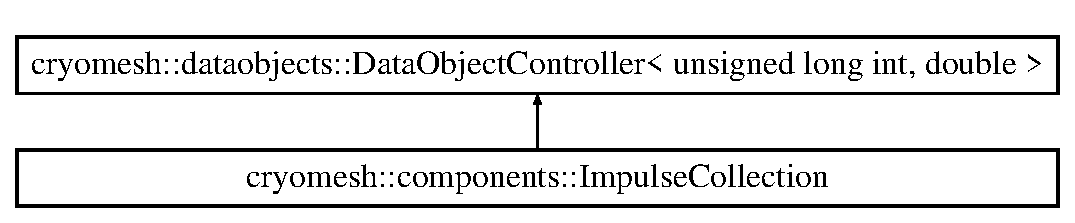
\includegraphics[height=2.000000cm]{classcryomesh_1_1components_1_1ImpulseCollection}
\end{center}
\end{figure}
\subsection*{\-Public \-Types}
\begin{DoxyCompactItemize}
\item 
enum \hyperlink{classcryomesh_1_1components_1_1ImpulseCollection_a3682719f1c0bd471e8c5a19b39cc285d}{\-Comparison} \{ \*
\hyperlink{classcryomesh_1_1components_1_1ImpulseCollection_a3682719f1c0bd471e8c5a19b39cc285da5288e1792a76693414517164a2289ec8}{\-Greater\-Than}, 
\hyperlink{classcryomesh_1_1components_1_1ImpulseCollection_a3682719f1c0bd471e8c5a19b39cc285da049307d079370521e85998e7141ec3af}{\-Less\-Than}, 
\hyperlink{classcryomesh_1_1components_1_1ImpulseCollection_a3682719f1c0bd471e8c5a19b39cc285da591330a7a512ed11c4429536a5d1e6d5}{\-Equal\-To}, 
\hyperlink{classcryomesh_1_1components_1_1ImpulseCollection_a3682719f1c0bd471e8c5a19b39cc285da1402ae2e51bdcd9c25fae0dbb70e0b7a}{\-Not\-Equal\-To}, 
\*
\hyperlink{classcryomesh_1_1components_1_1ImpulseCollection_a3682719f1c0bd471e8c5a19b39cc285dabb82adff3882cdd74faaef695b6bc82d}{\-Less\-Than\-Or\-Equal\-To}, 
\hyperlink{classcryomesh_1_1components_1_1ImpulseCollection_a3682719f1c0bd471e8c5a19b39cc285da5c716b8625dde68ad195d063f37be1d1}{\-Greater\-Than\-Or\-Equal\-To}
 \}
\end{DoxyCompactItemize}
\subsection*{\-Public \-Member \-Functions}
\begin{DoxyCompactItemize}
\item 
\hyperlink{classcryomesh_1_1components_1_1ImpulseCollection_a230de3cb1f60f8eba8a53237af529ed2}{\-Impulse\-Collection} ()
\begin{DoxyCompactList}\small\item\em \-Contructor for \hyperlink{classcryomesh_1_1components_1_1ImpulseCollection}{\-Impulse\-Collection}. \end{DoxyCompactList}\item 
virtual \hyperlink{classcryomesh_1_1components_1_1ImpulseCollection_a91bdcfc982090f9c665d5d8b80b8d3b9}{$\sim$\-Impulse\-Collection} ()
\begin{DoxyCompactList}\small\item\em \-Destructor for \hyperlink{classcryomesh_1_1components_1_1ImpulseCollection}{\-Impulse\-Collection}. \end{DoxyCompactList}\item 
double \hyperlink{classcryomesh_1_1components_1_1ImpulseCollection_ac9f6be8ecad07258e2c7b25efaa3df70}{get\-Activity} (\hyperlink{classcryomesh_1_1common_1_1Cycle}{common\-::\-Cycle} cycle) const 
\begin{DoxyCompactList}\small\item\em \-Get activity at cycle. \end{DoxyCompactList}\item 
double \hyperlink{classcryomesh_1_1components_1_1ImpulseCollection_acf0a767c00f141a2caee02a36aea6569}{get\-Activity} () const 
\begin{DoxyCompactList}\small\item\em \-Get activity at current cycle. \end{DoxyCompactList}\item 
void \hyperlink{classcryomesh_1_1components_1_1ImpulseCollection_ad465e66e8b49debd309bed6c8ca5bedb}{clear\-Impulses} ()
\begin{DoxyCompactList}\small\item\em \-Clear collection up to present cycle. \end{DoxyCompactList}\item 
void \hyperlink{classcryomesh_1_1components_1_1ImpulseCollection_a07c7c16d3a12c1f65dcb1686578d19da}{clear\-Impulses} (\hyperlink{classcryomesh_1_1common_1_1Cycle}{common\-::\-Cycle} cycle)
\begin{DoxyCompactList}\small\item\em \-Clear collection up to specified cycle. \end{DoxyCompactList}\item 
std\-::map$<$ boost\-::uuids\-::uuid, \*
boost\-::shared\-\_\-ptr$<$ \hyperlink{classcryomesh_1_1components_1_1Impulse}{\-Impulse} $>$ $>$ \hyperlink{classcryomesh_1_1components_1_1ImpulseCollection_abe07a298df807be2c62eadf976e02027}{clear\-Impulses} (\hyperlink{classcryomesh_1_1common_1_1Cycle}{common\-::\-Cycle} cycle\-Start, \hyperlink{classcryomesh_1_1common_1_1Cycle}{common\-::\-Cycle} cycle\-End)
\begin{DoxyCompactList}\small\item\em \-Clear the \-Impulses that start on or after cycle start parameter and finish before cycle end parameter. \end{DoxyCompactList}\item 
std\-::map$<$ boost\-::uuids\-::uuid, \*
boost\-::shared\-\_\-ptr$<$ \hyperlink{classcryomesh_1_1components_1_1Impulse}{\-Impulse} $>$ $>$ \hyperlink{classcryomesh_1_1components_1_1ImpulseCollection_a13560031007e894ea8d8d6cb0bdf48ff}{clear\-Active\-Impulses} ()
\begin{DoxyCompactList}\small\item\em \-Clear cycles that are active on this cycle. \end{DoxyCompactList}\item 
std\-::map$<$ boost\-::uuids\-::uuid, \*
boost\-::shared\-\_\-ptr$<$ \hyperlink{classcryomesh_1_1components_1_1Impulse}{\-Impulse} $>$ $>$ \hyperlink{classcryomesh_1_1components_1_1ImpulseCollection_a34f24b20735831c72fb4db04d014cff3}{clear\-Active\-Impulses} (\hyperlink{classcryomesh_1_1common_1_1Cycle}{common\-::\-Cycle} cycle)
\begin{DoxyCompactList}\small\item\em \-Clear cycles that are active on cycle. \end{DoxyCompactList}\item 
std\-::map$<$ boost\-::uuids\-::uuid, \*
boost\-::shared\-\_\-ptr$<$ \hyperlink{classcryomesh_1_1components_1_1Impulse}{\-Impulse} $>$ $>$ \hyperlink{classcryomesh_1_1components_1_1ImpulseCollection_a79fffb878409aff462a5fe9b1c1917f8}{clear\-Active\-Impulses} (\hyperlink{classcryomesh_1_1common_1_1Cycle}{common\-::\-Cycle} cycle\-Start, \hyperlink{classcryomesh_1_1common_1_1Cycle}{common\-::\-Cycle} cycle\-End)
\begin{DoxyCompactList}\small\item\em \-Clear cycles that are active on cycle range. \end{DoxyCompactList}\item 
std\-::map$<$ boost\-::uuids\-::uuid, \*
boost\-::shared\-\_\-ptr$<$ \hyperlink{classcryomesh_1_1components_1_1Impulse}{\-Impulse} $>$ $>$ \hyperlink{classcryomesh_1_1components_1_1ImpulseCollection_ab27eb4667bdb58c98e6614712f3b7373}{clear\-Activities\-By\-Minimum} (double activity)
\begin{DoxyCompactList}\small\item\em \-Clear the \-Impulses that have activities less than parameter. \end{DoxyCompactList}\item 
std\-::map$<$ boost\-::uuids\-::uuid, \*
boost\-::shared\-\_\-ptr$<$ \hyperlink{classcryomesh_1_1components_1_1Impulse}{\-Impulse} $>$ $>$ \hyperlink{classcryomesh_1_1components_1_1ImpulseCollection_a30ac8a9f8a401faf8277dd948ed2be15}{clear\-Activities\-By\-Maximum} (double activity)
\begin{DoxyCompactList}\small\item\em \-Clear the \-Impulses that have activities greater than parameter. \end{DoxyCompactList}\item 
void \hyperlink{classcryomesh_1_1components_1_1ImpulseCollection_a44ba846c61ae3d39730bd141072dc8e9}{decrement\-Activity\-Timers} ()
\begin{DoxyCompactList}\small\item\em \-Decrement the activity timers of all impulses. \end{DoxyCompactList}\item 
std\-::list$<$ boost\-::shared\-\_\-ptr\*
$<$ \hyperlink{classcryomesh_1_1components_1_1Impulse}{\-Impulse} $>$ $>$ \hyperlink{classcryomesh_1_1components_1_1ImpulseCollection_aea52c674f13597d808ad3e5f4f4bb9c1}{get\-By\-Activity\-Timer\-Value} (double value, \hyperlink{classcryomesh_1_1components_1_1ImpulseCollection_a3682719f1c0bd471e8c5a19b39cc285d}{\-Comparison} comp)
\begin{DoxyCompactList}\small\item\em \-Get impulse list by activity timer value. \end{DoxyCompactList}\item 
std\-::list$<$ boost\-::shared\-\_\-ptr\*
$<$ \hyperlink{classcryomesh_1_1components_1_1Impulse}{\-Impulse} $>$ $>$ \hyperlink{classcryomesh_1_1components_1_1ImpulseCollection_a317b84fe238bd4ff6bb8eda97b35cf1a}{remove\-By\-Activity\-Timer\-Value} (double value=0, \hyperlink{classcryomesh_1_1components_1_1ImpulseCollection_a3682719f1c0bd471e8c5a19b39cc285d}{\-Comparison} comp=\hyperlink{classcryomesh_1_1components_1_1ImpulseCollection_a3682719f1c0bd471e8c5a19b39cc285dabb82adff3882cdd74faaef695b6bc82d}{\-Less\-Than\-Or\-Equal\-To})
\begin{DoxyCompactList}\small\item\em remove impulses by activity timer value \end{DoxyCompactList}\item 
virtual void \hyperlink{classcryomesh_1_1components_1_1ImpulseCollection_a892cc1028a9539de15668c39511adba3}{refresh\-Data\-Object} ()
\begin{DoxyCompactList}\small\item\em \-Inherited from \-Data\-Object\-Controller. \end{DoxyCompactList}\item 
virtual void \hyperlink{classcryomesh_1_1components_1_1ImpulseCollection_a3e6df4eb108bd6e5acc6abe4184912b8}{enable\-Debug} (bool b)
\item 
\hyperlink{classcryomesh_1_1components_1_1ImpulseCollection}{\-Impulse\-Collection} \& \hyperlink{classcryomesh_1_1components_1_1ImpulseCollection_af2f41361cb06d4e6a4028e7ad9ba4792}{operator=} (const \hyperlink{classcryomesh_1_1components_1_1ImpulseCollection}{\-Impulse\-Collection} \&obj)
\begin{DoxyCompactList}\small\item\em \-Assignment operator. \end{DoxyCompactList}\item 
\hyperlink{classcryomesh_1_1components_1_1ImpulseCollection}{\-Impulse\-Collection} \& \hyperlink{classcryomesh_1_1components_1_1ImpulseCollection_a92954d37e3ef80ead5205fc5b288925e}{operator+=} (const \hyperlink{classcryomesh_1_1components_1_1ImpulseCollection}{\-Impulse\-Collection} \&obj)
\begin{DoxyCompactList}\small\item\em \-Destructive addition and assignment operator. \end{DoxyCompactList}\item 
const \hyperlink{classcryomesh_1_1components_1_1ImpulseCollection}{\-Impulse\-Collection} \hyperlink{classcryomesh_1_1components_1_1ImpulseCollection_af3e0802e865b4de8c005d749953c0102}{operator+} (const \hyperlink{classcryomesh_1_1components_1_1ImpulseCollection}{\-Impulse\-Collection} \&obj) const 
\begin{DoxyCompactList}\small\item\em \-Non-\/destructive addition operator. \end{DoxyCompactList}\item 
bool \hyperlink{classcryomesh_1_1components_1_1ImpulseCollection_a68b0c4b2aa6b213d0e579cad2cb920af}{operator==} (const \hyperlink{classcryomesh_1_1components_1_1ImpulseCollection}{\-Impulse\-Collection} \&obj) const 
\begin{DoxyCompactList}\small\item\em \-Comparator operator. \end{DoxyCompactList}\item 
bool \hyperlink{classcryomesh_1_1components_1_1ImpulseCollection_a64e8ed03f0ef6b33a0a94331bef08b05}{operator!=} (const \hyperlink{classcryomesh_1_1components_1_1ImpulseCollection}{\-Impulse\-Collection} \&obj) const 
\begin{DoxyCompactList}\small\item\em \-Not comparator operator. \end{DoxyCompactList}\item 
virtual void \hyperlink{classcryomesh_1_1dataobjects_1_1DataObjectController_a3e510413675407ec0a6745345ca9a3a8}{enable\-Logging} (bool enable)
\begin{DoxyCompactList}\small\item\em \-Whether logging is enabled or not. \end{DoxyCompactList}\item 
virtual const std\-::map\*
$<$ unsigned long int, double $>$ \& \hyperlink{classcryomesh_1_1dataobjects_1_1DataObjectController_a70a03ee28392ecf2e039702a18511f05}{get\-Map} ()
\begin{DoxyCompactList}\small\item\em \-Get all cycle values. \end{DoxyCompactList}\item 
virtual const \*
\hyperlink{classcryomesh_1_1dataobjects_1_1DataObject}{dataobjects\-::\-Data\-Object}\*
$<$ unsigned long int, double $>$ \& \hyperlink{classcryomesh_1_1dataobjects_1_1DataObjectController_aa919e8676a611028c6b6e6791c87f438}{get\-Data\-Object} ()
\begin{DoxyCompactList}\small\item\em \-Get data object. \end{DoxyCompactList}\end{DoxyCompactItemize}
\subsection*{\-Protected \-Member \-Functions}
\begin{DoxyCompactItemize}
\item 
std\-::map$<$ boost\-::uuids\-::uuid, \*
boost\-::shared\-\_\-ptr$<$ \hyperlink{classcryomesh_1_1components_1_1Impulse}{\-Impulse} $>$ $>$ \hyperlink{classcryomesh_1_1components_1_1ImpulseCollection_a3d5bac577752316e38d0d54715b85dca}{clear\-Activities\-By\-Value} (double activity, bool greater)
\begin{DoxyCompactList}\small\item\em \-Get the associated \-Mesh. \end{DoxyCompactList}\end{DoxyCompactItemize}
\subsection*{\-Protected \-Attributes}
\begin{DoxyCompactItemize}
\item 
\hyperlink{classcryomesh_1_1dataobjects_1_1DataObject}{dataobjects\-::\-Data\-Object}\*
$<$ unsigned long int, double $>$ \hyperlink{classcryomesh_1_1dataobjects_1_1DataObjectController_aa13d30e9fa2f1caa0510635214d4bb26}{data\-Object}
\end{DoxyCompactItemize}
\subsection*{\-Friends}
\begin{DoxyCompactItemize}
\item 
std\-::ostream \& \hyperlink{classcryomesh_1_1components_1_1ImpulseCollection_a7c219e0c7bb5a54301e5655d28f8a81b}{operator$<$$<$} (std\-::ostream \&os, const \hyperlink{classcryomesh_1_1components_1_1ImpulseCollection}{\-Impulse\-Collection} \&obj)
\begin{DoxyCompactList}\small\item\em \-To stream operator. \end{DoxyCompactList}\end{DoxyCompactItemize}


\subsection{\-Detailed \-Description}
\hyperlink{classcryomesh_1_1components_1_1ImpulseCollection}{\-Impulse\-Collection} represents a collection of \hyperlink{classcryomesh_1_1components_1_1Impulse}{\-Impulse} objects. 

\-A collection of \-Impulses that allows for \-Impulses to be held, 'moved forward' in time, and summated in some way 

\-Definition at line 35 of file \-Impulse\-Collection.\-h.



\subsection{\-Member \-Enumeration \-Documentation}
\hypertarget{classcryomesh_1_1components_1_1ImpulseCollection_a3682719f1c0bd471e8c5a19b39cc285d}{\index{cryomesh\-::components\-::\-Impulse\-Collection@{cryomesh\-::components\-::\-Impulse\-Collection}!\-Comparison@{\-Comparison}}
\index{\-Comparison@{\-Comparison}!cryomesh::components::ImpulseCollection@{cryomesh\-::components\-::\-Impulse\-Collection}}
\subsubsection[{\-Comparison}]{\setlength{\rightskip}{0pt plus 5cm}enum {\bf cryomesh\-::components\-::\-Impulse\-Collection\-::\-Comparison}}}\label{classcryomesh_1_1components_1_1ImpulseCollection_a3682719f1c0bd471e8c5a19b39cc285d}
\begin{Desc}
\item[\-Enumerator\-: ]\par
\begin{description}
\index{\-Greater\-Than@{\-Greater\-Than}!cryomesh\-::components\-::\-Impulse\-Collection@{cryomesh\-::components\-::\-Impulse\-Collection}}\index{cryomesh\-::components\-::\-Impulse\-Collection@{cryomesh\-::components\-::\-Impulse\-Collection}!\-Greater\-Than@{\-Greater\-Than}}\item[{\em 
\hypertarget{classcryomesh_1_1components_1_1ImpulseCollection_a3682719f1c0bd471e8c5a19b39cc285da5288e1792a76693414517164a2289ec8}{\-Greater\-Than}\label{classcryomesh_1_1components_1_1ImpulseCollection_a3682719f1c0bd471e8c5a19b39cc285da5288e1792a76693414517164a2289ec8}
}]\index{\-Less\-Than@{\-Less\-Than}!cryomesh\-::components\-::\-Impulse\-Collection@{cryomesh\-::components\-::\-Impulse\-Collection}}\index{cryomesh\-::components\-::\-Impulse\-Collection@{cryomesh\-::components\-::\-Impulse\-Collection}!\-Less\-Than@{\-Less\-Than}}\item[{\em 
\hypertarget{classcryomesh_1_1components_1_1ImpulseCollection_a3682719f1c0bd471e8c5a19b39cc285da049307d079370521e85998e7141ec3af}{\-Less\-Than}\label{classcryomesh_1_1components_1_1ImpulseCollection_a3682719f1c0bd471e8c5a19b39cc285da049307d079370521e85998e7141ec3af}
}]\index{\-Equal\-To@{\-Equal\-To}!cryomesh\-::components\-::\-Impulse\-Collection@{cryomesh\-::components\-::\-Impulse\-Collection}}\index{cryomesh\-::components\-::\-Impulse\-Collection@{cryomesh\-::components\-::\-Impulse\-Collection}!\-Equal\-To@{\-Equal\-To}}\item[{\em 
\hypertarget{classcryomesh_1_1components_1_1ImpulseCollection_a3682719f1c0bd471e8c5a19b39cc285da591330a7a512ed11c4429536a5d1e6d5}{\-Equal\-To}\label{classcryomesh_1_1components_1_1ImpulseCollection_a3682719f1c0bd471e8c5a19b39cc285da591330a7a512ed11c4429536a5d1e6d5}
}]\index{\-Not\-Equal\-To@{\-Not\-Equal\-To}!cryomesh\-::components\-::\-Impulse\-Collection@{cryomesh\-::components\-::\-Impulse\-Collection}}\index{cryomesh\-::components\-::\-Impulse\-Collection@{cryomesh\-::components\-::\-Impulse\-Collection}!\-Not\-Equal\-To@{\-Not\-Equal\-To}}\item[{\em 
\hypertarget{classcryomesh_1_1components_1_1ImpulseCollection_a3682719f1c0bd471e8c5a19b39cc285da1402ae2e51bdcd9c25fae0dbb70e0b7a}{\-Not\-Equal\-To}\label{classcryomesh_1_1components_1_1ImpulseCollection_a3682719f1c0bd471e8c5a19b39cc285da1402ae2e51bdcd9c25fae0dbb70e0b7a}
}]\index{\-Less\-Than\-Or\-Equal\-To@{\-Less\-Than\-Or\-Equal\-To}!cryomesh\-::components\-::\-Impulse\-Collection@{cryomesh\-::components\-::\-Impulse\-Collection}}\index{cryomesh\-::components\-::\-Impulse\-Collection@{cryomesh\-::components\-::\-Impulse\-Collection}!\-Less\-Than\-Or\-Equal\-To@{\-Less\-Than\-Or\-Equal\-To}}\item[{\em 
\hypertarget{classcryomesh_1_1components_1_1ImpulseCollection_a3682719f1c0bd471e8c5a19b39cc285dabb82adff3882cdd74faaef695b6bc82d}{\-Less\-Than\-Or\-Equal\-To}\label{classcryomesh_1_1components_1_1ImpulseCollection_a3682719f1c0bd471e8c5a19b39cc285dabb82adff3882cdd74faaef695b6bc82d}
}]\index{\-Greater\-Than\-Or\-Equal\-To@{\-Greater\-Than\-Or\-Equal\-To}!cryomesh\-::components\-::\-Impulse\-Collection@{cryomesh\-::components\-::\-Impulse\-Collection}}\index{cryomesh\-::components\-::\-Impulse\-Collection@{cryomesh\-::components\-::\-Impulse\-Collection}!\-Greater\-Than\-Or\-Equal\-To@{\-Greater\-Than\-Or\-Equal\-To}}\item[{\em 
\hypertarget{classcryomesh_1_1components_1_1ImpulseCollection_a3682719f1c0bd471e8c5a19b39cc285da5c716b8625dde68ad195d063f37be1d1}{\-Greater\-Than\-Or\-Equal\-To}\label{classcryomesh_1_1components_1_1ImpulseCollection_a3682719f1c0bd471e8c5a19b39cc285da5c716b8625dde68ad195d063f37be1d1}
}]\end{description}
\end{Desc}



\-Definition at line 38 of file \-Impulse\-Collection.\-h.



\subsection{\-Constructor \& \-Destructor \-Documentation}
\hypertarget{classcryomesh_1_1components_1_1ImpulseCollection_a230de3cb1f60f8eba8a53237af529ed2}{\index{cryomesh\-::components\-::\-Impulse\-Collection@{cryomesh\-::components\-::\-Impulse\-Collection}!\-Impulse\-Collection@{\-Impulse\-Collection}}
\index{\-Impulse\-Collection@{\-Impulse\-Collection}!cryomesh::components::ImpulseCollection@{cryomesh\-::components\-::\-Impulse\-Collection}}
\subsubsection[{\-Impulse\-Collection}]{\setlength{\rightskip}{0pt plus 5cm}{\bf cryomesh\-::components\-::\-Impulse\-Collection\-::\-Impulse\-Collection} (
\begin{DoxyParamCaption}
{}
\end{DoxyParamCaption}
)}}\label{classcryomesh_1_1components_1_1ImpulseCollection_a230de3cb1f60f8eba8a53237af529ed2}


\-Contructor for \hyperlink{classcryomesh_1_1components_1_1ImpulseCollection}{\-Impulse\-Collection}. 

\-Contruct using default \-Mesh 

\-Definition at line 18 of file \-Impulse\-Collection.\-cpp.

\hypertarget{classcryomesh_1_1components_1_1ImpulseCollection_a91bdcfc982090f9c665d5d8b80b8d3b9}{\index{cryomesh\-::components\-::\-Impulse\-Collection@{cryomesh\-::components\-::\-Impulse\-Collection}!$\sim$\-Impulse\-Collection@{$\sim$\-Impulse\-Collection}}
\index{$\sim$\-Impulse\-Collection@{$\sim$\-Impulse\-Collection}!cryomesh::components::ImpulseCollection@{cryomesh\-::components\-::\-Impulse\-Collection}}
\subsubsection[{$\sim$\-Impulse\-Collection}]{\setlength{\rightskip}{0pt plus 5cm}{\bf cryomesh\-::components\-::\-Impulse\-Collection\-::$\sim$\-Impulse\-Collection} (
\begin{DoxyParamCaption}
{}
\end{DoxyParamCaption}
)\hspace{0.3cm}{\ttfamily  \mbox{[}virtual\mbox{]}}}}\label{classcryomesh_1_1components_1_1ImpulseCollection_a91bdcfc982090f9c665d5d8b80b8d3b9}


\-Destructor for \hyperlink{classcryomesh_1_1components_1_1ImpulseCollection}{\-Impulse\-Collection}. 

\-Destructor 

\-Definition at line 22 of file \-Impulse\-Collection.\-cpp.



\subsection{\-Member \-Function \-Documentation}
\hypertarget{classcryomesh_1_1components_1_1ImpulseCollection_a13560031007e894ea8d8d6cb0bdf48ff}{\index{cryomesh\-::components\-::\-Impulse\-Collection@{cryomesh\-::components\-::\-Impulse\-Collection}!clear\-Active\-Impulses@{clear\-Active\-Impulses}}
\index{clear\-Active\-Impulses@{clear\-Active\-Impulses}!cryomesh::components::ImpulseCollection@{cryomesh\-::components\-::\-Impulse\-Collection}}
\subsubsection[{clear\-Active\-Impulses}]{\setlength{\rightskip}{0pt plus 5cm}std\-::map$<$ boost\-::uuids\-::uuid, boost\-::shared\-\_\-ptr$<$ {\bf \-Impulse} $>$ $>$ {\bf cryomesh\-::components\-::\-Impulse\-Collection\-::clear\-Active\-Impulses} (
\begin{DoxyParamCaption}
{}
\end{DoxyParamCaption}
)}}\label{classcryomesh_1_1components_1_1ImpulseCollection_a13560031007e894ea8d8d6cb0bdf48ff}


\-Clear cycles that are active on this cycle. 

\-Update the collection to by dropping all impulses that are active on this cycle

\begin{DoxyReturn}{\-Returns}
std\-::map$<$boost\-::uuids\-::uuid, boost\-::shared\-\_\-ptr$<$\-Impulse$>$ $>$ \-The collection of deleted impulses 
\end{DoxyReturn}


\-Definition at line 122 of file \-Impulse\-Collection.\-cpp.



\-References cryomesh\-::common\-::\-Time\-Keeper\-::get\-Time\-Keeper().



\-Referenced by clear\-Active\-Impulses(), cryomesh\-::components\-::\-Node\-::enter\-Recovery(), and cryomesh\-::components\-::\-Node\-::update().

\hypertarget{classcryomesh_1_1components_1_1ImpulseCollection_a34f24b20735831c72fb4db04d014cff3}{\index{cryomesh\-::components\-::\-Impulse\-Collection@{cryomesh\-::components\-::\-Impulse\-Collection}!clear\-Active\-Impulses@{clear\-Active\-Impulses}}
\index{clear\-Active\-Impulses@{clear\-Active\-Impulses}!cryomesh::components::ImpulseCollection@{cryomesh\-::components\-::\-Impulse\-Collection}}
\subsubsection[{clear\-Active\-Impulses}]{\setlength{\rightskip}{0pt plus 5cm}std\-::map$<$ boost\-::uuids\-::uuid, boost\-::shared\-\_\-ptr$<$ {\bf \-Impulse} $>$ $>$ {\bf cryomesh\-::components\-::\-Impulse\-Collection\-::clear\-Active\-Impulses} (
\begin{DoxyParamCaption}
\item[{{\bf common\-::\-Cycle}}]{cycle}
\end{DoxyParamCaption}
)}}\label{classcryomesh_1_1components_1_1ImpulseCollection_a34f24b20735831c72fb4db04d014cff3}


\-Clear cycles that are active on cycle. 

\-Update the collection to by dropping all impulses that are active on cycle


\begin{DoxyParams}{\-Parameters}
{\em \hyperlink{classcryomesh_1_1common_1_1Cycle}{common\-::\-Cycle}} & cycle \-The cycle to drop inclusive impulses from\\
\hline
\end{DoxyParams}
\begin{DoxyReturn}{\-Returns}
std\-::map$<$boost\-::uuids\-::uuid, boost\-::shared\-\_\-ptr$<$\-Impulse$>$ $>$ \-The collection of deleted impulses 
\end{DoxyReturn}


\-Definition at line 127 of file \-Impulse\-Collection.\-cpp.



\-References clear\-Active\-Impulses().

\hypertarget{classcryomesh_1_1components_1_1ImpulseCollection_a79fffb878409aff462a5fe9b1c1917f8}{\index{cryomesh\-::components\-::\-Impulse\-Collection@{cryomesh\-::components\-::\-Impulse\-Collection}!clear\-Active\-Impulses@{clear\-Active\-Impulses}}
\index{clear\-Active\-Impulses@{clear\-Active\-Impulses}!cryomesh::components::ImpulseCollection@{cryomesh\-::components\-::\-Impulse\-Collection}}
\subsubsection[{clear\-Active\-Impulses}]{\setlength{\rightskip}{0pt plus 5cm}std\-::map$<$ boost\-::uuids\-::uuid, boost\-::shared\-\_\-ptr$<$ {\bf \-Impulse} $>$ $>$ {\bf cryomesh\-::components\-::\-Impulse\-Collection\-::clear\-Active\-Impulses} (
\begin{DoxyParamCaption}
\item[{{\bf common\-::\-Cycle}}]{cycle\-Start, }
\item[{{\bf common\-::\-Cycle}}]{cycle\-End}
\end{DoxyParamCaption}
)}}\label{classcryomesh_1_1components_1_1ImpulseCollection_a79fffb878409aff462a5fe9b1c1917f8}


\-Clear cycles that are active on cycle range. 

\-Interval is \mbox{[}cycle\-\_\-start,cycle\-\_\-end)

\-Update the collection to by dropping all impulses that are active on cycle range


\begin{DoxyParams}{\-Parameters}
{\em \hyperlink{classcryomesh_1_1common_1_1Cycle}{common\-::\-Cycle}} & cycle\-Start \-The start cycle to drop inclusive impulses from \\
\hline
{\em \hyperlink{classcryomesh_1_1common_1_1Cycle}{common\-::\-Cycle}} & cycle\-End \-The end cycle to drop inclusive impulses from excluded\\
\hline
\end{DoxyParams}
\begin{DoxyReturn}{\-Returns}
std\-::map$<$boost\-::uuids\-::uuid, boost\-::shared\-\_\-ptr$<$\-Impulse$>$ $>$ \-The collection of deleted impulses 
\end{DoxyReturn}


\-Definition at line 131 of file \-Impulse\-Collection.\-cpp.



\-References cryomesh\-::common\-::\-Time\-Keeper\-::get\-Cycle(), cryomesh\-::components\-::\-Impulse\-::get\-First\-Active\-Cycle(), cryomesh\-::components\-::\-Impulse\-::get\-Last\-Active\-Cycle(), cryomesh\-::common\-::\-Time\-Keeper\-::get\-Time\-Keeper(), and cryomesh\-::components\-::\-Impulse\-::is\-Active().

\hypertarget{classcryomesh_1_1components_1_1ImpulseCollection_a30ac8a9f8a401faf8277dd948ed2be15}{\index{cryomesh\-::components\-::\-Impulse\-Collection@{cryomesh\-::components\-::\-Impulse\-Collection}!clear\-Activities\-By\-Maximum@{clear\-Activities\-By\-Maximum}}
\index{clear\-Activities\-By\-Maximum@{clear\-Activities\-By\-Maximum}!cryomesh::components::ImpulseCollection@{cryomesh\-::components\-::\-Impulse\-Collection}}
\subsubsection[{clear\-Activities\-By\-Maximum}]{\setlength{\rightskip}{0pt plus 5cm}std\-::map$<$ boost\-::uuids\-::uuid, boost\-::shared\-\_\-ptr$<$ {\bf \-Impulse} $>$ $>$ {\bf cryomesh\-::components\-::\-Impulse\-Collection\-::clear\-Activities\-By\-Maximum} (
\begin{DoxyParamCaption}
\item[{double}]{activity}
\end{DoxyParamCaption}
)}}\label{classcryomesh_1_1components_1_1ImpulseCollection_a30ac8a9f8a401faf8277dd948ed2be15}


\-Clear the \-Impulses that have activities greater than parameter. 


\begin{DoxyParams}{\-Parameters}
{\em double} & activity \-The maximum activity impulses must have to avoid deleteion\\
\hline
\end{DoxyParams}
\begin{DoxyReturn}{\-Returns}
std\-::map$<$boost\-::uuids\-::uuid, boost\-::shared\-\_\-ptr$<$\-Impulse$>$ $>$ \-The deleted collection of impulses 
\end{DoxyReturn}


\-Definition at line 188 of file \-Impulse\-Collection.\-cpp.



\-References clear\-Activities\-By\-Value().

\hypertarget{classcryomesh_1_1components_1_1ImpulseCollection_ab27eb4667bdb58c98e6614712f3b7373}{\index{cryomesh\-::components\-::\-Impulse\-Collection@{cryomesh\-::components\-::\-Impulse\-Collection}!clear\-Activities\-By\-Minimum@{clear\-Activities\-By\-Minimum}}
\index{clear\-Activities\-By\-Minimum@{clear\-Activities\-By\-Minimum}!cryomesh::components::ImpulseCollection@{cryomesh\-::components\-::\-Impulse\-Collection}}
\subsubsection[{clear\-Activities\-By\-Minimum}]{\setlength{\rightskip}{0pt plus 5cm}std\-::map$<$ boost\-::uuids\-::uuid, boost\-::shared\-\_\-ptr$<$ {\bf \-Impulse} $>$ $>$ {\bf cryomesh\-::components\-::\-Impulse\-Collection\-::clear\-Activities\-By\-Minimum} (
\begin{DoxyParamCaption}
\item[{double}]{activity}
\end{DoxyParamCaption}
)}}\label{classcryomesh_1_1components_1_1ImpulseCollection_ab27eb4667bdb58c98e6614712f3b7373}


\-Clear the \-Impulses that have activities less than parameter. 


\begin{DoxyParams}{\-Parameters}
{\em double} & activity \-The minimum activity impulses must have to avoid deleteion\\
\hline
\end{DoxyParams}
\begin{DoxyReturn}{\-Returns}
std\-::map$<$boost\-::uuids\-::uuid, boost\-::shared\-\_\-ptr$<$\-Impulse$>$ $>$ \-The deleted collection of impulses 
\end{DoxyReturn}


\-Definition at line 184 of file \-Impulse\-Collection.\-cpp.



\-References clear\-Activities\-By\-Value().

\hypertarget{classcryomesh_1_1components_1_1ImpulseCollection_a3d5bac577752316e38d0d54715b85dca}{\index{cryomesh\-::components\-::\-Impulse\-Collection@{cryomesh\-::components\-::\-Impulse\-Collection}!clear\-Activities\-By\-Value@{clear\-Activities\-By\-Value}}
\index{clear\-Activities\-By\-Value@{clear\-Activities\-By\-Value}!cryomesh::components::ImpulseCollection@{cryomesh\-::components\-::\-Impulse\-Collection}}
\subsubsection[{clear\-Activities\-By\-Value}]{\setlength{\rightskip}{0pt plus 5cm}std\-::map$<$ boost\-::uuids\-::uuid, boost\-::shared\-\_\-ptr$<$ {\bf \-Impulse} $>$ $>$ {\bf cryomesh\-::components\-::\-Impulse\-Collection\-::clear\-Activities\-By\-Value} (
\begin{DoxyParamCaption}
\item[{double}]{activity, }
\item[{bool}]{greater}
\end{DoxyParamCaption}
)\hspace{0.3cm}{\ttfamily  \mbox{[}protected\mbox{]}}}}\label{classcryomesh_1_1components_1_1ImpulseCollection_a3d5bac577752316e38d0d54715b85dca}


\-Get the associated \-Mesh. 

\begin{DoxyReturn}{\-Returns}
\-Mesh
\end{DoxyReturn}
const boost\-::shared\-\_\-ptr$<$\-Mesh$>$ get\-Mesh() const; \-Clear the \-Impulses that have activities greater or less than parameter


\begin{DoxyParams}{\-Parameters}
{\em double} & activity \-The maximum or minimum activity impulses must have to avoid deleteion \\
\hline
{\em bool} & \-True is first parameter is maximum allowed value, false if its the minimum\\
\hline
\end{DoxyParams}
\begin{DoxyReturn}{\-Returns}
std\-::map$<$boost\-::uuids\-::uuid, boost\-::shared\-\_\-ptr$<$\-Impulse$>$ $>$ \-The deleted collection of impulses 
\end{DoxyReturn}


\-Definition at line 400 of file \-Impulse\-Collection.\-cpp.



\-Referenced by clear\-Activities\-By\-Maximum(), and clear\-Activities\-By\-Minimum().

\hypertarget{classcryomesh_1_1components_1_1ImpulseCollection_ad465e66e8b49debd309bed6c8ca5bedb}{\index{cryomesh\-::components\-::\-Impulse\-Collection@{cryomesh\-::components\-::\-Impulse\-Collection}!clear\-Impulses@{clear\-Impulses}}
\index{clear\-Impulses@{clear\-Impulses}!cryomesh::components::ImpulseCollection@{cryomesh\-::components\-::\-Impulse\-Collection}}
\subsubsection[{clear\-Impulses}]{\setlength{\rightskip}{0pt plus 5cm}void {\bf cryomesh\-::components\-::\-Impulse\-Collection\-::clear\-Impulses} (
\begin{DoxyParamCaption}
{}
\end{DoxyParamCaption}
)}}\label{classcryomesh_1_1components_1_1ImpulseCollection_ad465e66e8b49debd309bed6c8ca5bedb}


\-Clear collection up to present cycle. 

\-Update the collection to present cycle (non-\/inclusive) by dropping all impulses that are 'in the past' relative to that cycle. \-Interval is \mbox{[}0,present\-\_\-cycle) 

\-Definition at line 56 of file \-Impulse\-Collection.\-cpp.



\-References cryomesh\-::common\-::\-Time\-Keeper\-::get\-Cycle(), and cryomesh\-::common\-::\-Time\-Keeper\-::get\-Time\-Keeper().



\-Referenced by clear\-Impulses(), and cryomesh\-::components\-::\-Node\-::update\-Impulses().

\hypertarget{classcryomesh_1_1components_1_1ImpulseCollection_a07c7c16d3a12c1f65dcb1686578d19da}{\index{cryomesh\-::components\-::\-Impulse\-Collection@{cryomesh\-::components\-::\-Impulse\-Collection}!clear\-Impulses@{clear\-Impulses}}
\index{clear\-Impulses@{clear\-Impulses}!cryomesh::components::ImpulseCollection@{cryomesh\-::components\-::\-Impulse\-Collection}}
\subsubsection[{clear\-Impulses}]{\setlength{\rightskip}{0pt plus 5cm}void {\bf cryomesh\-::components\-::\-Impulse\-Collection\-::clear\-Impulses} (
\begin{DoxyParamCaption}
\item[{{\bf common\-::\-Cycle}}]{cycle}
\end{DoxyParamCaption}
)}}\label{classcryomesh_1_1components_1_1ImpulseCollection_a07c7c16d3a12c1f65dcb1686578d19da}


\-Clear collection up to specified cycle. 

\-Update the collection to specified cycle (non-\/inclusive) by dropping all impulses that are 'in the past' relative to that cycle. \-Interval is \mbox{[}0,cycle)


\begin{DoxyParams}{\-Parameters}
{\em \hyperlink{classcryomesh_1_1common_1_1Cycle}{common\-::\-Cycle}} & cycle \-The cycle that is the cutoff point for the collection \\
\hline
\end{DoxyParams}


\-Definition at line 60 of file \-Impulse\-Collection.\-cpp.



\-References clear\-Impulses().

\hypertarget{classcryomesh_1_1components_1_1ImpulseCollection_abe07a298df807be2c62eadf976e02027}{\index{cryomesh\-::components\-::\-Impulse\-Collection@{cryomesh\-::components\-::\-Impulse\-Collection}!clear\-Impulses@{clear\-Impulses}}
\index{clear\-Impulses@{clear\-Impulses}!cryomesh::components::ImpulseCollection@{cryomesh\-::components\-::\-Impulse\-Collection}}
\subsubsection[{clear\-Impulses}]{\setlength{\rightskip}{0pt plus 5cm}std\-::map$<$ boost\-::uuids\-::uuid, boost\-::shared\-\_\-ptr$<$ {\bf \-Impulse} $>$ $>$ {\bf cryomesh\-::components\-::\-Impulse\-Collection\-::clear\-Impulses} (
\begin{DoxyParamCaption}
\item[{{\bf common\-::\-Cycle}}]{cycle\-Start, }
\item[{{\bf common\-::\-Cycle}}]{cycle\-End}
\end{DoxyParamCaption}
)}}\label{classcryomesh_1_1components_1_1ImpulseCollection_abe07a298df807be2c62eadf976e02027}


\-Clear the \-Impulses that start on or after cycle start parameter and finish before cycle end parameter. 

\-Interval is \mbox{[}cycle\-\_\-start,cycle\-\_\-end)


\begin{DoxyParams}{\-Parameters}
{\em \-Cycle} & cycle\-Start \-Cycle parameter that marks the start of the cleared area \\
\hline
{\em \-Cycle} & cycle\-End \-Cycle parameter that marks the end of the cleared area (non-\/inclusive)\\
\hline
\end{DoxyParams}
\begin{DoxyReturn}{\-Returns}
std\-::map$<$boost\-::uuids\-::uuid, boost\-::shared\-\_\-ptr$<$\-Impulse$>$ $>$ \-The deleted collection of impulses 
\end{DoxyReturn}


\-Definition at line 64 of file \-Impulse\-Collection.\-cpp.



\-References cryomesh\-::common\-::\-Time\-Keeper\-::get\-Cycle(), and cryomesh\-::common\-::\-Time\-Keeper\-::get\-Time\-Keeper().

\hypertarget{classcryomesh_1_1components_1_1ImpulseCollection_a44ba846c61ae3d39730bd141072dc8e9}{\index{cryomesh\-::components\-::\-Impulse\-Collection@{cryomesh\-::components\-::\-Impulse\-Collection}!decrement\-Activity\-Timers@{decrement\-Activity\-Timers}}
\index{decrement\-Activity\-Timers@{decrement\-Activity\-Timers}!cryomesh::components::ImpulseCollection@{cryomesh\-::components\-::\-Impulse\-Collection}}
\subsubsection[{decrement\-Activity\-Timers}]{\setlength{\rightskip}{0pt plus 5cm}void {\bf cryomesh\-::components\-::\-Impulse\-Collection\-::decrement\-Activity\-Timers} (
\begin{DoxyParamCaption}
{}
\end{DoxyParamCaption}
)}}\label{classcryomesh_1_1components_1_1ImpulseCollection_a44ba846c61ae3d39730bd141072dc8e9}


\-Decrement the activity timers of all impulses. 



\-Definition at line 192 of file \-Impulse\-Collection.\-cpp.



\-Referenced by cryomesh\-::components\-::\-Connection\-::update().

\hypertarget{classcryomesh_1_1components_1_1ImpulseCollection_a3e6df4eb108bd6e5acc6abe4184912b8}{\index{cryomesh\-::components\-::\-Impulse\-Collection@{cryomesh\-::components\-::\-Impulse\-Collection}!enable\-Debug@{enable\-Debug}}
\index{enable\-Debug@{enable\-Debug}!cryomesh::components::ImpulseCollection@{cryomesh\-::components\-::\-Impulse\-Collection}}
\subsubsection[{enable\-Debug}]{\setlength{\rightskip}{0pt plus 5cm}void {\bf cryomesh\-::components\-::\-Impulse\-Collection\-::enable\-Debug} (
\begin{DoxyParamCaption}
\item[{bool}]{b}
\end{DoxyParamCaption}
)\hspace{0.3cm}{\ttfamily  \mbox{[}virtual\mbox{]}}}}\label{classcryomesh_1_1components_1_1ImpulseCollection_a3e6df4eb108bd6e5acc6abe4184912b8}


\-Definition at line 320 of file \-Impulse\-Collection.\-cpp.

\hypertarget{classcryomesh_1_1dataobjects_1_1DataObjectController_a3e510413675407ec0a6745345ca9a3a8}{\index{cryomesh\-::components\-::\-Impulse\-Collection@{cryomesh\-::components\-::\-Impulse\-Collection}!enable\-Logging@{enable\-Logging}}
\index{enable\-Logging@{enable\-Logging}!cryomesh::components::ImpulseCollection@{cryomesh\-::components\-::\-Impulse\-Collection}}
\subsubsection[{enable\-Logging}]{\setlength{\rightskip}{0pt plus 5cm}virtual void {\bf cryomesh\-::dataobjects\-::\-Data\-Object\-Controller}$<$ unsigned long int , double  $>$\-::{\bf enable\-Logging} (
\begin{DoxyParamCaption}
\item[{bool}]{enable}
\end{DoxyParamCaption}
)\hspace{0.3cm}{\ttfamily  \mbox{[}inline, virtual, inherited\mbox{]}}}}\label{classcryomesh_1_1dataobjects_1_1DataObjectController_a3e510413675407ec0a6745345ca9a3a8}


\-Whether logging is enabled or not. 


\begin{DoxyParams}{\-Parameters}
{\em bool} & enable \-True to enable logging, false otherwise \\
\hline
\end{DoxyParams}


\-Definition at line 47 of file \-Data\-Object\-Controller.\-h.



\-References cryomesh\-::dataobjects\-::\-Data\-Object\-Controller$<$ U, T $>$\-::data\-Object.

\hypertarget{classcryomesh_1_1components_1_1ImpulseCollection_ac9f6be8ecad07258e2c7b25efaa3df70}{\index{cryomesh\-::components\-::\-Impulse\-Collection@{cryomesh\-::components\-::\-Impulse\-Collection}!get\-Activity@{get\-Activity}}
\index{get\-Activity@{get\-Activity}!cryomesh::components::ImpulseCollection@{cryomesh\-::components\-::\-Impulse\-Collection}}
\subsubsection[{get\-Activity}]{\setlength{\rightskip}{0pt plus 5cm}double {\bf cryomesh\-::components\-::\-Impulse\-Collection\-::get\-Activity} (
\begin{DoxyParamCaption}
\item[{{\bf common\-::\-Cycle}}]{cycle}
\end{DoxyParamCaption}
) const}}\label{classcryomesh_1_1components_1_1ImpulseCollection_ac9f6be8ecad07258e2c7b25efaa3df70}


\-Get activity at cycle. 

\-Sum all the \-Impulses in the collection on specified cycle and return activity


\begin{DoxyParams}{\-Parameters}
{\em \-Cycle} & cycle \-The cycle to calculate the activity on\\
\hline
\end{DoxyParams}
\begin{DoxyReturn}{\-Returns}
double \-The activity on specified cycle 
\end{DoxyReturn}


\-Definition at line 25 of file \-Impulse\-Collection.\-cpp.



\-Referenced by cryomesh\-::components\-::\-Node\-::get\-Activity().

\hypertarget{classcryomesh_1_1components_1_1ImpulseCollection_acf0a767c00f141a2caee02a36aea6569}{\index{cryomesh\-::components\-::\-Impulse\-Collection@{cryomesh\-::components\-::\-Impulse\-Collection}!get\-Activity@{get\-Activity}}
\index{get\-Activity@{get\-Activity}!cryomesh::components::ImpulseCollection@{cryomesh\-::components\-::\-Impulse\-Collection}}
\subsubsection[{get\-Activity}]{\setlength{\rightskip}{0pt plus 5cm}double {\bf cryomesh\-::components\-::\-Impulse\-Collection\-::get\-Activity} (
\begin{DoxyParamCaption}
{}
\end{DoxyParamCaption}
) const}}\label{classcryomesh_1_1components_1_1ImpulseCollection_acf0a767c00f141a2caee02a36aea6569}


\-Get activity at current cycle. 

\-Sum all the \-Impulses in the collection on the current cycle and return activity

\begin{DoxyReturn}{\-Returns}
double \-The activity on specified cycle 
\end{DoxyReturn}


\-Definition at line 51 of file \-Impulse\-Collection.\-cpp.



\-References cryomesh\-::common\-::\-Time\-Keeper\-::get\-Cycle(), and cryomesh\-::common\-::\-Time\-Keeper\-::get\-Time\-Keeper().



\-Referenced by refresh\-Data\-Object().

\hypertarget{classcryomesh_1_1components_1_1ImpulseCollection_aea52c674f13597d808ad3e5f4f4bb9c1}{\index{cryomesh\-::components\-::\-Impulse\-Collection@{cryomesh\-::components\-::\-Impulse\-Collection}!get\-By\-Activity\-Timer\-Value@{get\-By\-Activity\-Timer\-Value}}
\index{get\-By\-Activity\-Timer\-Value@{get\-By\-Activity\-Timer\-Value}!cryomesh::components::ImpulseCollection@{cryomesh\-::components\-::\-Impulse\-Collection}}
\subsubsection[{get\-By\-Activity\-Timer\-Value}]{\setlength{\rightskip}{0pt plus 5cm}std\-::list$<$ boost\-::shared\-\_\-ptr$<$ {\bf \-Impulse} $>$ $>$ {\bf cryomesh\-::components\-::\-Impulse\-Collection\-::get\-By\-Activity\-Timer\-Value} (
\begin{DoxyParamCaption}
\item[{double}]{value, }
\item[{{\bf \-Impulse\-Collection\-::\-Comparison}}]{comp}
\end{DoxyParamCaption}
)}}\label{classcryomesh_1_1components_1_1ImpulseCollection_aea52c674f13597d808ad3e5f4f4bb9c1}


\-Get impulse list by activity timer value. 


\begin{DoxyParams}{\-Parameters}
{\em double} & value activity timer value \\
\hline
{\em \-Comparison} & comp \-What comparison to make with the value\\
\hline
\end{DoxyParams}
\begin{DoxyReturn}{\-Returns}
std\-::list$<$boost\-::shared\-\_\-ptr$<$ Impulse$>$ $>$ \-The list of impulses that meet the comparison 
\end{DoxyReturn}


\-Definition at line 208 of file \-Impulse\-Collection.\-cpp.



\-References \-Equal\-To, \-Greater\-Than, \-Greater\-Than\-Or\-Equal\-To, \-Less\-Than, and \-Less\-Than\-Or\-Equal\-To.



\-Referenced by remove\-By\-Activity\-Timer\-Value().

\hypertarget{classcryomesh_1_1dataobjects_1_1DataObjectController_aa919e8676a611028c6b6e6791c87f438}{\index{cryomesh\-::components\-::\-Impulse\-Collection@{cryomesh\-::components\-::\-Impulse\-Collection}!get\-Data\-Object@{get\-Data\-Object}}
\index{get\-Data\-Object@{get\-Data\-Object}!cryomesh::components::ImpulseCollection@{cryomesh\-::components\-::\-Impulse\-Collection}}
\subsubsection[{get\-Data\-Object}]{\setlength{\rightskip}{0pt plus 5cm}virtual const {\bf dataobjects\-::\-Data\-Object}$<$unsigned long int , double $>$\& {\bf cryomesh\-::dataobjects\-::\-Data\-Object\-Controller}$<$ unsigned long int , double  $>$\-::{\bf get\-Data\-Object} (
\begin{DoxyParamCaption}
{}
\end{DoxyParamCaption}
)\hspace{0.3cm}{\ttfamily  \mbox{[}inline, virtual, inherited\mbox{]}}}}\label{classcryomesh_1_1dataobjects_1_1DataObjectController_aa919e8676a611028c6b6e6791c87f438}


\-Get data object. 

\begin{DoxyReturn}{\-Returns}
dataobjects\-::\-Data\-Object$<$\-U,\-T$>$ \& \-The data object 
\end{DoxyReturn}


\-Definition at line 68 of file \-Data\-Object\-Controller.\-h.



\-References cryomesh\-::dataobjects\-::\-Data\-Object\-Controller$<$ U, T $>$\-::data\-Object, and cryomesh\-::dataobjects\-::\-Data\-Object\-Controller$<$ U, T $>$\-::refresh\-Data\-Object().

\hypertarget{classcryomesh_1_1dataobjects_1_1DataObjectController_a70a03ee28392ecf2e039702a18511f05}{\index{cryomesh\-::components\-::\-Impulse\-Collection@{cryomesh\-::components\-::\-Impulse\-Collection}!get\-Map@{get\-Map}}
\index{get\-Map@{get\-Map}!cryomesh::components::ImpulseCollection@{cryomesh\-::components\-::\-Impulse\-Collection}}
\subsubsection[{get\-Map}]{\setlength{\rightskip}{0pt plus 5cm}virtual const std\-::map$<$unsigned long int , double $>$\& {\bf cryomesh\-::dataobjects\-::\-Data\-Object\-Controller}$<$ unsigned long int , double  $>$\-::{\bf get\-Map} (
\begin{DoxyParamCaption}
{}
\end{DoxyParamCaption}
)\hspace{0.3cm}{\ttfamily  \mbox{[}inline, virtual, inherited\mbox{]}}}}\label{classcryomesh_1_1dataobjects_1_1DataObjectController_a70a03ee28392ecf2e039702a18511f05}


\-Get all cycle values. 

\begin{DoxyReturn}{\-Returns}
std\-::map$<$unsigned long int, double$>$ \& \-The cycle values 
\end{DoxyReturn}


\-Definition at line 57 of file \-Data\-Object\-Controller.\-h.



\-References cryomesh\-::dataobjects\-::\-Data\-Object\-Controller$<$ U, T $>$\-::data\-Object, and cryomesh\-::dataobjects\-::\-Data\-Object\-Controller$<$ U, T $>$\-::refresh\-Data\-Object().

\hypertarget{classcryomesh_1_1components_1_1ImpulseCollection_a64e8ed03f0ef6b33a0a94331bef08b05}{\index{cryomesh\-::components\-::\-Impulse\-Collection@{cryomesh\-::components\-::\-Impulse\-Collection}!operator!=@{operator!=}}
\index{operator!=@{operator!=}!cryomesh::components::ImpulseCollection@{cryomesh\-::components\-::\-Impulse\-Collection}}
\subsubsection[{operator!=}]{\setlength{\rightskip}{0pt plus 5cm}bool cryomesh\-::components\-::\-Impulse\-Collection\-::operator!= (
\begin{DoxyParamCaption}
\item[{const {\bf \-Impulse\-Collection} \&}]{obj}
\end{DoxyParamCaption}
) const}}\label{classcryomesh_1_1components_1_1ImpulseCollection_a64e8ed03f0ef6b33a0a94331bef08b05}


\-Not comparator operator. 


\begin{DoxyParams}{\-Parameters}
{\em const} & \hyperlink{classcryomesh_1_1components_1_1ImpulseCollection}{\-Impulse\-Collection} \& obj \-R\-H\-S object\\
\hline
\end{DoxyParams}
\begin{DoxyReturn}{\-Returns}
bool \-True if not equal, false otherwise 
\end{DoxyReturn}


\-Definition at line 371 of file \-Impulse\-Collection.\-cpp.

\hypertarget{classcryomesh_1_1components_1_1ImpulseCollection_af3e0802e865b4de8c005d749953c0102}{\index{cryomesh\-::components\-::\-Impulse\-Collection@{cryomesh\-::components\-::\-Impulse\-Collection}!operator+@{operator+}}
\index{operator+@{operator+}!cryomesh::components::ImpulseCollection@{cryomesh\-::components\-::\-Impulse\-Collection}}
\subsubsection[{operator+}]{\setlength{\rightskip}{0pt plus 5cm}const {\bf \-Impulse\-Collection} cryomesh\-::components\-::\-Impulse\-Collection\-::operator+ (
\begin{DoxyParamCaption}
\item[{const {\bf \-Impulse\-Collection} \&}]{obj}
\end{DoxyParamCaption}
) const}}\label{classcryomesh_1_1components_1_1ImpulseCollection_af3e0802e865b4de8c005d749953c0102}


\-Non-\/destructive addition operator. 


\begin{DoxyParams}{\-Parameters}
{\em const} & \hyperlink{classcryomesh_1_1components_1_1ImpulseCollection}{\-Impulse\-Collection} \& obj \-R\-H\-S addition\\
\hline
\end{DoxyParams}
\begin{DoxyReturn}{\-Returns}
\hyperlink{classcryomesh_1_1components_1_1ImpulseCollection}{\-Impulse\-Collection} \-New object after addition 
\end{DoxyReturn}


\-Definition at line 314 of file \-Impulse\-Collection.\-cpp.

\hypertarget{classcryomesh_1_1components_1_1ImpulseCollection_a92954d37e3ef80ead5205fc5b288925e}{\index{cryomesh\-::components\-::\-Impulse\-Collection@{cryomesh\-::components\-::\-Impulse\-Collection}!operator+=@{operator+=}}
\index{operator+=@{operator+=}!cryomesh::components::ImpulseCollection@{cryomesh\-::components\-::\-Impulse\-Collection}}
\subsubsection[{operator+=}]{\setlength{\rightskip}{0pt plus 5cm}{\bf \-Impulse\-Collection} \& cryomesh\-::components\-::\-Impulse\-Collection\-::operator+= (
\begin{DoxyParamCaption}
\item[{const {\bf \-Impulse\-Collection} \&}]{obj}
\end{DoxyParamCaption}
)}}\label{classcryomesh_1_1components_1_1ImpulseCollection_a92954d37e3ef80ead5205fc5b288925e}


\-Destructive addition and assignment operator. 


\begin{DoxyParams}{\-Parameters}
{\em const} & \hyperlink{classcryomesh_1_1components_1_1ImpulseCollection}{\-Impulse\-Collection} \& obj \-R\-H\-S addition\\
\hline
\end{DoxyParams}
\begin{DoxyReturn}{\-Returns}
\hyperlink{classcryomesh_1_1components_1_1ImpulseCollection}{\-Impulse\-Collection} \& \-This object after addition and assignment 
\end{DoxyReturn}


\-Definition at line 294 of file \-Impulse\-Collection.\-cpp.

\hypertarget{classcryomesh_1_1components_1_1ImpulseCollection_af2f41361cb06d4e6a4028e7ad9ba4792}{\index{cryomesh\-::components\-::\-Impulse\-Collection@{cryomesh\-::components\-::\-Impulse\-Collection}!operator=@{operator=}}
\index{operator=@{operator=}!cryomesh::components::ImpulseCollection@{cryomesh\-::components\-::\-Impulse\-Collection}}
\subsubsection[{operator=}]{\setlength{\rightskip}{0pt plus 5cm}{\bf \-Impulse\-Collection} \& cryomesh\-::components\-::\-Impulse\-Collection\-::operator= (
\begin{DoxyParamCaption}
\item[{const {\bf \-Impulse\-Collection} \&}]{obj}
\end{DoxyParamCaption}
)}}\label{classcryomesh_1_1components_1_1ImpulseCollection_af2f41361cb06d4e6a4028e7ad9ba4792}


\-Assignment operator. 


\begin{DoxyParams}{\-Parameters}
{\em const} & \hyperlink{classcryomesh_1_1components_1_1ImpulseCollection}{\-Impulse\-Collection} \& obj \-R\-H\-S assignment\\
\hline
\end{DoxyParams}
\begin{DoxyReturn}{\-Returns}
\hyperlink{classcryomesh_1_1components_1_1ImpulseCollection}{\-Impulse\-Collection} \& \-This object after assignment 
\end{DoxyReturn}


\-Definition at line 285 of file \-Impulse\-Collection.\-cpp.

\hypertarget{classcryomesh_1_1components_1_1ImpulseCollection_a68b0c4b2aa6b213d0e579cad2cb920af}{\index{cryomesh\-::components\-::\-Impulse\-Collection@{cryomesh\-::components\-::\-Impulse\-Collection}!operator==@{operator==}}
\index{operator==@{operator==}!cryomesh::components::ImpulseCollection@{cryomesh\-::components\-::\-Impulse\-Collection}}
\subsubsection[{operator==}]{\setlength{\rightskip}{0pt plus 5cm}bool cryomesh\-::components\-::\-Impulse\-Collection\-::operator== (
\begin{DoxyParamCaption}
\item[{const {\bf \-Impulse\-Collection} \&}]{obj}
\end{DoxyParamCaption}
) const}}\label{classcryomesh_1_1components_1_1ImpulseCollection_a68b0c4b2aa6b213d0e579cad2cb920af}


\-Comparator operator. 


\begin{DoxyParams}{\-Parameters}
{\em const} & \hyperlink{classcryomesh_1_1components_1_1ImpulseCollection}{\-Impulse\-Collection} \& obj \-R\-H\-S object\\
\hline
\end{DoxyParams}
\begin{DoxyReturn}{\-Returns}
bool \-True if equal, false otherwise 
\end{DoxyReturn}


\-Definition at line 324 of file \-Impulse\-Collection.\-cpp.

\hypertarget{classcryomesh_1_1components_1_1ImpulseCollection_a892cc1028a9539de15668c39511adba3}{\index{cryomesh\-::components\-::\-Impulse\-Collection@{cryomesh\-::components\-::\-Impulse\-Collection}!refresh\-Data\-Object@{refresh\-Data\-Object}}
\index{refresh\-Data\-Object@{refresh\-Data\-Object}!cryomesh::components::ImpulseCollection@{cryomesh\-::components\-::\-Impulse\-Collection}}
\subsubsection[{refresh\-Data\-Object}]{\setlength{\rightskip}{0pt plus 5cm}void {\bf cryomesh\-::components\-::\-Impulse\-Collection\-::refresh\-Data\-Object} (
\begin{DoxyParamCaption}
{}
\end{DoxyParamCaption}
)\hspace{0.3cm}{\ttfamily  \mbox{[}virtual\mbox{]}}}}\label{classcryomesh_1_1components_1_1ImpulseCollection_a892cc1028a9539de15668c39511adba3}


\-Inherited from \-Data\-Object\-Controller. 

\-Overriden to force refresh update on call 

\-Reimplemented from \hyperlink{classcryomesh_1_1dataobjects_1_1DataObjectController_ae015efe3d10cced82d5043f560cbe04f}{cryomesh\-::dataobjects\-::\-Data\-Object\-Controller$<$ unsigned long int, double $>$}.



\-Definition at line 265 of file \-Impulse\-Collection.\-cpp.



\-References cryomesh\-::dataobjects\-::\-Data\-Object$<$ U, T $>$\-::clear(), cryomesh\-::dataobjects\-::\-Data\-Object\-Controller$<$ unsigned long int, double $>$\-::data\-Object, get\-Activity(), cryomesh\-::common\-::\-Time\-Keeper\-::get\-Cycle(), cryomesh\-::dataobjects\-::\-Data\-Object$<$ U, T $>$\-::get\-Dataset\-Maximum\-Size(), cryomesh\-::common\-::\-Time\-Keeper\-::get\-Time\-Keeper(), cryomesh\-::dataobjects\-::\-Data\-Object$<$ U, T $>$\-::insert(), cryomesh\-::dataobjects\-::\-Data\-Object$<$ U, T $>$\-::is\-Logging\-Enabled(), and cryomesh\-::common\-::\-Cycle\-::to\-U\-L\-Int().

\hypertarget{classcryomesh_1_1components_1_1ImpulseCollection_a317b84fe238bd4ff6bb8eda97b35cf1a}{\index{cryomesh\-::components\-::\-Impulse\-Collection@{cryomesh\-::components\-::\-Impulse\-Collection}!remove\-By\-Activity\-Timer\-Value@{remove\-By\-Activity\-Timer\-Value}}
\index{remove\-By\-Activity\-Timer\-Value@{remove\-By\-Activity\-Timer\-Value}!cryomesh::components::ImpulseCollection@{cryomesh\-::components\-::\-Impulse\-Collection}}
\subsubsection[{remove\-By\-Activity\-Timer\-Value}]{\setlength{\rightskip}{0pt plus 5cm}std\-::list$<$ boost\-::shared\-\_\-ptr$<$ {\bf \-Impulse} $>$ $>$ {\bf cryomesh\-::components\-::\-Impulse\-Collection\-::remove\-By\-Activity\-Timer\-Value} (
\begin{DoxyParamCaption}
\item[{double}]{value = {\ttfamily 0}, }
\item[{{\bf \-Impulse\-Collection\-::\-Comparison}}]{comp = {\ttfamily {\bf \-Less\-Than\-Or\-Equal\-To}}}
\end{DoxyParamCaption}
)}}\label{classcryomesh_1_1components_1_1ImpulseCollection_a317b84fe238bd4ff6bb8eda97b35cf1a}


remove impulses by activity timer value 


\begin{DoxyParams}{\-Parameters}
{\em double} & value activity timer value \\
\hline
{\em \-Comparison} & comp \-What comparison to make with the value\\
\hline
\end{DoxyParams}
\begin{DoxyReturn}{\-Returns}
std\-::list$<$boost\-::shared\-\_\-ptr$<$ Impulse$>$ $>$ \-The that meet the comparison and were removed 
\end{DoxyReturn}


\-Definition at line 258 of file \-Impulse\-Collection.\-cpp.



\-References get\-By\-Activity\-Timer\-Value().



\-Referenced by cryomesh\-::components\-::\-Connection\-::update().



\subsection{\-Friends \-And \-Related \-Function \-Documentation}
\hypertarget{classcryomesh_1_1components_1_1ImpulseCollection_a7c219e0c7bb5a54301e5655d28f8a81b}{\index{cryomesh\-::components\-::\-Impulse\-Collection@{cryomesh\-::components\-::\-Impulse\-Collection}!operator$<$$<$@{operator$<$$<$}}
\index{operator$<$$<$@{operator$<$$<$}!cryomesh::components::ImpulseCollection@{cryomesh\-::components\-::\-Impulse\-Collection}}
\subsubsection[{operator$<$$<$}]{\setlength{\rightskip}{0pt plus 5cm}std\-::ostream\& operator$<$$<$ (
\begin{DoxyParamCaption}
\item[{std\-::ostream \&}]{os, }
\item[{const {\bf \-Impulse\-Collection} \&}]{obj}
\end{DoxyParamCaption}
)\hspace{0.3cm}{\ttfamily  \mbox{[}friend\mbox{]}}}}\label{classcryomesh_1_1components_1_1ImpulseCollection_a7c219e0c7bb5a54301e5655d28f8a81b}


\-To stream operator. 


\begin{DoxyParams}{\-Parameters}
{\em std\-::ostream} & \& os \-The output stream \\
\hline
{\em const} & \hyperlink{classcryomesh_1_1components_1_1ImpulseCollection}{\-Impulse\-Collection} \& obj \-The object to stream\\
\hline
\end{DoxyParams}
\begin{DoxyReturn}{\-Returns}
std\-::ostream \& \-The output stream 
\end{DoxyReturn}


\-Definition at line 375 of file \-Impulse\-Collection.\-cpp.



\subsection{\-Member \-Data \-Documentation}
\hypertarget{classcryomesh_1_1dataobjects_1_1DataObjectController_aa13d30e9fa2f1caa0510635214d4bb26}{\index{cryomesh\-::components\-::\-Impulse\-Collection@{cryomesh\-::components\-::\-Impulse\-Collection}!data\-Object@{data\-Object}}
\index{data\-Object@{data\-Object}!cryomesh::components::ImpulseCollection@{cryomesh\-::components\-::\-Impulse\-Collection}}
\subsubsection[{data\-Object}]{\setlength{\rightskip}{0pt plus 5cm}{\bf dataobjects\-::\-Data\-Object}$<$unsigned long int , double $>$ {\bf cryomesh\-::dataobjects\-::\-Data\-Object\-Controller}$<$ unsigned long int , double  $>$\-::{\bf data\-Object}\hspace{0.3cm}{\ttfamily  \mbox{[}protected, inherited\mbox{]}}}}\label{classcryomesh_1_1dataobjects_1_1DataObjectController_aa13d30e9fa2f1caa0510635214d4bb26}


\-Definition at line 85 of file \-Data\-Object\-Controller.\-h.



\-Referenced by refresh\-Data\-Object(), and cryomesh\-::components\-::\-Node\-::update().



\-The documentation for this class was generated from the following files\-:\begin{DoxyCompactItemize}
\item 
/home/niall/\-Projects/\-Eclipse/\-C\-P\-P/cryomesh/src/components/\hyperlink{ImpulseCollection_8h}{\-Impulse\-Collection.\-h}\item 
/home/niall/\-Projects/\-Eclipse/\-C\-P\-P/cryomesh/src/components/\hyperlink{ImpulseCollection_8cpp}{\-Impulse\-Collection.\-cpp}\end{DoxyCompactItemize}

\hypertarget{structcryomesh_1_1manager_1_1InputPatternsTableFormat}{\section{cryomesh\-:\-:manager\-:\-:\-Input\-Patterns\-Table\-Format \-Struct \-Reference}
\label{structcryomesh_1_1manager_1_1InputPatternsTableFormat}\index{cryomesh\-::manager\-::\-Input\-Patterns\-Table\-Format@{cryomesh\-::manager\-::\-Input\-Patterns\-Table\-Format}}
}


\-Struct representing input pattern table structure.  




{\ttfamily \#include $<$\-Table\-Formats.\-h$>$}

\-Inheritance diagram for cryomesh\-:\-:manager\-:\-:\-Input\-Patterns\-Table\-Format\-:\begin{figure}[H]
\begin{center}
\leavevmode
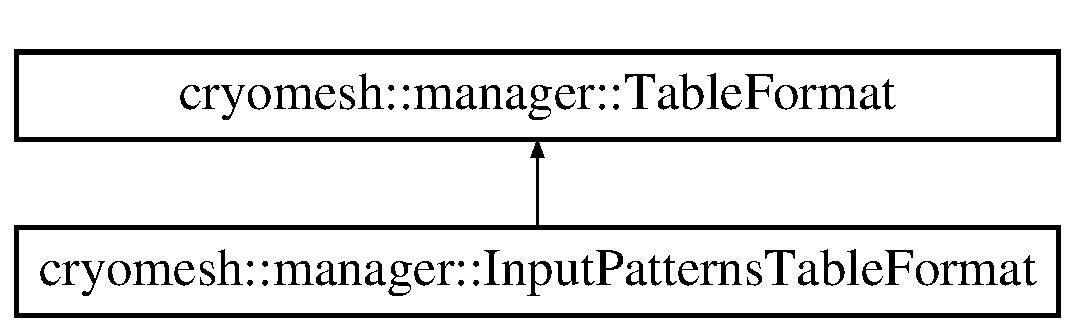
\includegraphics[height=2.000000cm]{structcryomesh_1_1manager_1_1InputPatternsTableFormat}
\end{center}
\end{figure}
\subsection*{\-Public \-Member \-Functions}
\begin{DoxyCompactItemize}
\item 
\hyperlink{structcryomesh_1_1manager_1_1InputPatternsTableFormat_a0e64ea9f3ebd45a2549b2edcfb226034}{\-Input\-Patterns\-Table\-Format} ()
\begin{DoxyCompactList}\small\item\em \-Default constructor will construct all the names and columns assiciated with a pattern table. \end{DoxyCompactList}\item 
std\-::string \hyperlink{structcryomesh_1_1manager_1_1TableFormat_a3e797d6130c6b0745a1fac799c25677a}{get\-Name} () const 
\begin{DoxyCompactList}\small\item\em \-Return the name of the table. \end{DoxyCompactList}\item 
std\-::string \hyperlink{structcryomesh_1_1manager_1_1TableFormat_a2256ce39471582b92bf7cbb6eec74d30}{get\-Key} (const std\-::string \&key)
\begin{DoxyCompactList}\small\item\em \-Return the string object associated with a key. \end{DoxyCompactList}\item 
std\-::string \hyperlink{structcryomesh_1_1manager_1_1TableFormat_a898ae0d0c5490ccdf71aec5156b10fcc}{get\-Create\-Table} () const 
\begin{DoxyCompactList}\small\item\em \-Get the string that can be used to create the sql table. \end{DoxyCompactList}\end{DoxyCompactItemize}
\subsection*{\-Protected \-Attributes}
\begin{DoxyCompactItemize}
\item 
std\-::string \hyperlink{structcryomesh_1_1manager_1_1TableFormat_ab49912897ccb7fd0f8d42f1cc21332e8}{name}
\item 
std\-::map$<$ std\-::string, \*
std\-::string $>$ \hyperlink{structcryomesh_1_1manager_1_1TableFormat_a29ab6f4cfc0c56da1fa461ea665a1b61}{columns}
\end{DoxyCompactItemize}


\subsection{\-Detailed \-Description}
\-Struct representing input pattern table structure. 

\-Definition at line 136 of file \-Table\-Formats.\-h.



\subsection{\-Constructor \& \-Destructor \-Documentation}
\hypertarget{structcryomesh_1_1manager_1_1InputPatternsTableFormat_a0e64ea9f3ebd45a2549b2edcfb226034}{\index{cryomesh\-::manager\-::\-Input\-Patterns\-Table\-Format@{cryomesh\-::manager\-::\-Input\-Patterns\-Table\-Format}!\-Input\-Patterns\-Table\-Format@{\-Input\-Patterns\-Table\-Format}}
\index{\-Input\-Patterns\-Table\-Format@{\-Input\-Patterns\-Table\-Format}!cryomesh::manager::InputPatternsTableFormat@{cryomesh\-::manager\-::\-Input\-Patterns\-Table\-Format}}
\subsubsection[{\-Input\-Patterns\-Table\-Format}]{\setlength{\rightskip}{0pt plus 5cm}{\bf cryomesh\-::manager\-::\-Input\-Patterns\-Table\-Format\-::\-Input\-Patterns\-Table\-Format} (
\begin{DoxyParamCaption}
{}
\end{DoxyParamCaption}
)\hspace{0.3cm}{\ttfamily  \mbox{[}inline\mbox{]}}}}\label{structcryomesh_1_1manager_1_1InputPatternsTableFormat_a0e64ea9f3ebd45a2549b2edcfb226034}


\-Default constructor will construct all the names and columns assiciated with a pattern table. 



\-Definition at line 141 of file \-Table\-Formats.\-h.



\-References cryomesh\-::manager\-::\-Table\-Format\-::columns, and cryomesh\-::manager\-::\-Table\-Format\-::name.



\subsection{\-Member \-Function \-Documentation}
\hypertarget{structcryomesh_1_1manager_1_1TableFormat_a898ae0d0c5490ccdf71aec5156b10fcc}{\index{cryomesh\-::manager\-::\-Input\-Patterns\-Table\-Format@{cryomesh\-::manager\-::\-Input\-Patterns\-Table\-Format}!get\-Create\-Table@{get\-Create\-Table}}
\index{get\-Create\-Table@{get\-Create\-Table}!cryomesh::manager::InputPatternsTableFormat@{cryomesh\-::manager\-::\-Input\-Patterns\-Table\-Format}}
\subsubsection[{get\-Create\-Table}]{\setlength{\rightskip}{0pt plus 5cm}std\-::string {\bf cryomesh\-::manager\-::\-Table\-Format\-::get\-Create\-Table} (
\begin{DoxyParamCaption}
{}
\end{DoxyParamCaption}
) const\hspace{0.3cm}{\ttfamily  \mbox{[}inline, inherited\mbox{]}}}}\label{structcryomesh_1_1manager_1_1TableFormat_a898ae0d0c5490ccdf71aec5156b10fcc}


\-Get the string that can be used to create the sql table. 

\begin{DoxyReturn}{\-Returns}
the sql command string to create this table 
\end{DoxyReturn}


\-Definition at line 60 of file \-Table\-Formats.\-h.



\-References cryomesh\-::manager\-::\-Table\-Format\-::columns, and cryomesh\-::manager\-::\-Table\-Format\-::get\-Name().

\hypertarget{structcryomesh_1_1manager_1_1TableFormat_a2256ce39471582b92bf7cbb6eec74d30}{\index{cryomesh\-::manager\-::\-Input\-Patterns\-Table\-Format@{cryomesh\-::manager\-::\-Input\-Patterns\-Table\-Format}!get\-Key@{get\-Key}}
\index{get\-Key@{get\-Key}!cryomesh::manager::InputPatternsTableFormat@{cryomesh\-::manager\-::\-Input\-Patterns\-Table\-Format}}
\subsubsection[{get\-Key}]{\setlength{\rightskip}{0pt plus 5cm}std\-::string {\bf cryomesh\-::manager\-::\-Table\-Format\-::get\-Key} (
\begin{DoxyParamCaption}
\item[{const std\-::string \&}]{key}
\end{DoxyParamCaption}
)\hspace{0.3cm}{\ttfamily  \mbox{[}inline, inherited\mbox{]}}}}\label{structcryomesh_1_1manager_1_1TableFormat_a2256ce39471582b92bf7cbb6eec74d30}


\-Return the string object associated with a key. 

\-::string \-The key to search for

\begin{DoxyReturn}{\-Returns}
std\-::string \-The object associated with the search key, \char`\"{}\char`\"{} if not found 
\end{DoxyReturn}


\-Definition at line 45 of file \-Table\-Formats.\-h.



\-References cryomesh\-::manager\-::\-Table\-Format\-::columns.

\hypertarget{structcryomesh_1_1manager_1_1TableFormat_a3e797d6130c6b0745a1fac799c25677a}{\index{cryomesh\-::manager\-::\-Input\-Patterns\-Table\-Format@{cryomesh\-::manager\-::\-Input\-Patterns\-Table\-Format}!get\-Name@{get\-Name}}
\index{get\-Name@{get\-Name}!cryomesh::manager::InputPatternsTableFormat@{cryomesh\-::manager\-::\-Input\-Patterns\-Table\-Format}}
\subsubsection[{get\-Name}]{\setlength{\rightskip}{0pt plus 5cm}std\-::string {\bf cryomesh\-::manager\-::\-Table\-Format\-::get\-Name} (
\begin{DoxyParamCaption}
{}
\end{DoxyParamCaption}
) const\hspace{0.3cm}{\ttfamily  \mbox{[}inline, inherited\mbox{]}}}}\label{structcryomesh_1_1manager_1_1TableFormat_a3e797d6130c6b0745a1fac799c25677a}


\-Return the name of the table. 

\begin{DoxyReturn}{\-Returns}
std\-::string \-The name of the table 
\end{DoxyReturn}


\-Definition at line 32 of file \-Table\-Formats.\-h.



\-References cryomesh\-::manager\-::\-Table\-Format\-::name.



\-Referenced by cryomesh\-::manager\-::\-Table\-Format\-::get\-Create\-Table(), cryomesh\-::manager\-::\-Database\-Manager\-::insert\-Connection(), cryomesh\-::manager\-::\-Database\-Manager\-::insert\-Node(), and cryomesh\-::manager\-::\-Database\-Manager\-::insert\-Output\-Pattern().



\subsection{\-Member \-Data \-Documentation}
\hypertarget{structcryomesh_1_1manager_1_1TableFormat_a29ab6f4cfc0c56da1fa461ea665a1b61}{\index{cryomesh\-::manager\-::\-Input\-Patterns\-Table\-Format@{cryomesh\-::manager\-::\-Input\-Patterns\-Table\-Format}!columns@{columns}}
\index{columns@{columns}!cryomesh::manager::InputPatternsTableFormat@{cryomesh\-::manager\-::\-Input\-Patterns\-Table\-Format}}
\subsubsection[{columns}]{\setlength{\rightskip}{0pt plus 5cm}std\-::map$<$std\-::string, std\-::string$>$ {\bf cryomesh\-::manager\-::\-Table\-Format\-::columns}\hspace{0.3cm}{\ttfamily  \mbox{[}protected, inherited\mbox{]}}}}\label{structcryomesh_1_1manager_1_1TableFormat_a29ab6f4cfc0c56da1fa461ea665a1b61}


\-Definition at line 93 of file \-Table\-Formats.\-h.



\-Referenced by cryomesh\-::manager\-::\-Connection\-Table\-Format\-::\-Connection\-Table\-Format(), cryomesh\-::manager\-::\-Table\-Format\-::get\-Create\-Table(), cryomesh\-::manager\-::\-Table\-Format\-::get\-Key(), \-Input\-Patterns\-Table\-Format(), cryomesh\-::manager\-::\-Node\-Table\-Format\-::\-Node\-Table\-Format(), and cryomesh\-::manager\-::\-Output\-Patterns\-Table\-Format\-::\-Output\-Patterns\-Table\-Format().

\hypertarget{structcryomesh_1_1manager_1_1TableFormat_ab49912897ccb7fd0f8d42f1cc21332e8}{\index{cryomesh\-::manager\-::\-Input\-Patterns\-Table\-Format@{cryomesh\-::manager\-::\-Input\-Patterns\-Table\-Format}!name@{name}}
\index{name@{name}!cryomesh::manager::InputPatternsTableFormat@{cryomesh\-::manager\-::\-Input\-Patterns\-Table\-Format}}
\subsubsection[{name}]{\setlength{\rightskip}{0pt plus 5cm}std\-::string {\bf cryomesh\-::manager\-::\-Table\-Format\-::name}\hspace{0.3cm}{\ttfamily  \mbox{[}protected, inherited\mbox{]}}}}\label{structcryomesh_1_1manager_1_1TableFormat_ab49912897ccb7fd0f8d42f1cc21332e8}


\-Definition at line 86 of file \-Table\-Formats.\-h.



\-Referenced by cryomesh\-::manager\-::\-Connection\-Table\-Format\-::\-Connection\-Table\-Format(), cryomesh\-::manager\-::\-Table\-Format\-::get\-Name(), \-Input\-Patterns\-Table\-Format(), cryomesh\-::manager\-::\-Node\-Table\-Format\-::\-Node\-Table\-Format(), and cryomesh\-::manager\-::\-Output\-Patterns\-Table\-Format\-::\-Output\-Patterns\-Table\-Format().



\-The documentation for this struct was generated from the following file\-:\begin{DoxyCompactItemize}
\item 
/home/niall/\-Projects/\-Eclipse/\-C\-P\-P/cryomesh/src/manager/\hyperlink{TableFormats_8h}{\-Table\-Formats.\-h}\end{DoxyCompactItemize}

\hypertarget{classcryomesh_1_1common_1_1Loggable}{\section{cryomesh\-:\-:common\-:\-:\-Loggable \-Class \-Reference}
\label{classcryomesh_1_1common_1_1Loggable}\index{cryomesh\-::common\-::\-Loggable@{cryomesh\-::common\-::\-Loggable}}
}


{\ttfamily \#include $<$\-Loggable.\-h$>$}

\-Inheritance diagram for cryomesh\-:\-:common\-:\-:\-Loggable\-:\begin{figure}[H]
\begin{center}
\leavevmode
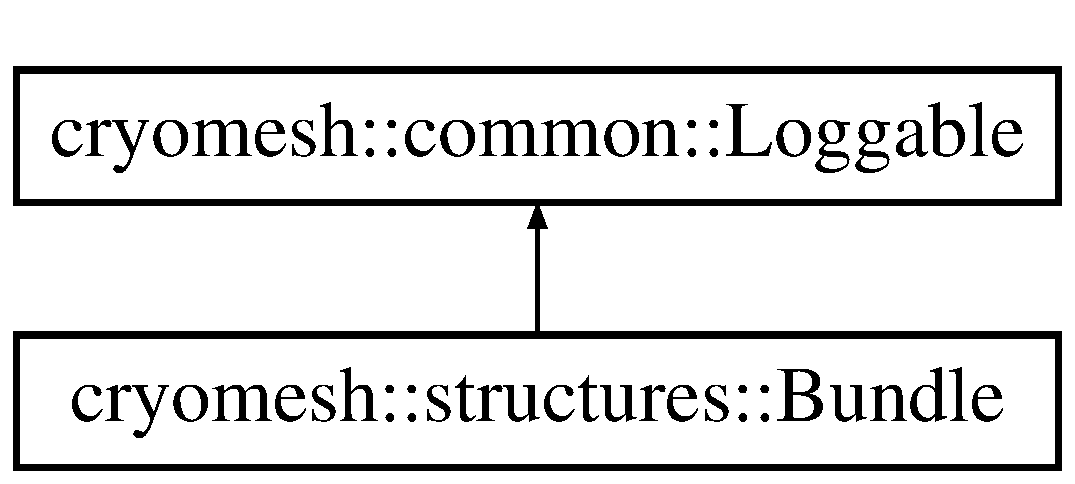
\includegraphics[height=2.000000cm]{classcryomesh_1_1common_1_1Loggable}
\end{center}
\end{figure}
\subsection*{\-Public \-Types}
\begin{DoxyCompactItemize}
\item 
enum \hyperlink{classcryomesh_1_1common_1_1Loggable_a4d85401f6c81bc8ed94e49d66ae574c5}{\-Logging\-Depth} \{ \hyperlink{classcryomesh_1_1common_1_1Loggable_a4d85401f6c81bc8ed94e49d66ae574c5a51f5abcf5a53a8930a09b065fc64a44f}{\-S\-U\-M\-M\-A\-R\-Y}, 
\hyperlink{classcryomesh_1_1common_1_1Loggable_a4d85401f6c81bc8ed94e49d66ae574c5ae496af0b41e3b64530b61e315822cc51}{\-M\-A\-X}
 \}
\begin{DoxyCompactList}\small\item\em \-Enum representing print detail. \end{DoxyCompactList}\end{DoxyCompactItemize}
\subsection*{\-Public \-Member \-Functions}
\begin{DoxyCompactItemize}
\item 
\hyperlink{classcryomesh_1_1common_1_1Loggable_a52e7934753ed7cc33972ed2fc57b571c}{\-Loggable} ()
\item 
virtual \hyperlink{classcryomesh_1_1common_1_1Loggable_a8295792cec325f663f0d6c64ec960cb2}{$\sim$\-Loggable} ()
\item 
virtual std\-::ostream \& \hyperlink{classcryomesh_1_1common_1_1Loggable_a8709b369a43141412e72786dba572dfd}{print} (std\-::ostream \&os, const \hyperlink{classcryomesh_1_1common_1_1Loggable_a4d85401f6c81bc8ed94e49d66ae574c5}{\-Loggable\-::\-Logging\-Depth} depth=\hyperlink{classcryomesh_1_1common_1_1Loggable_a4d85401f6c81bc8ed94e49d66ae574c5a51f5abcf5a53a8930a09b065fc64a44f}{\-Loggable\-::\-S\-U\-M\-M\-A\-R\-Y}) const =0
\end{DoxyCompactItemize}


\subsection{\-Detailed \-Description}


\-Definition at line 17 of file \-Loggable.\-h.



\subsection{\-Member \-Enumeration \-Documentation}
\hypertarget{classcryomesh_1_1common_1_1Loggable_a4d85401f6c81bc8ed94e49d66ae574c5}{\index{cryomesh\-::common\-::\-Loggable@{cryomesh\-::common\-::\-Loggable}!\-Logging\-Depth@{\-Logging\-Depth}}
\index{\-Logging\-Depth@{\-Logging\-Depth}!cryomesh::common::Loggable@{cryomesh\-::common\-::\-Loggable}}
\subsubsection[{\-Logging\-Depth}]{\setlength{\rightskip}{0pt plus 5cm}enum {\bf cryomesh\-::common\-::\-Loggable\-::\-Logging\-Depth}}}\label{classcryomesh_1_1common_1_1Loggable_a4d85401f6c81bc8ed94e49d66ae574c5}


\-Enum representing print detail. 

\begin{Desc}
\item[\-Enumerator\-: ]\par
\begin{description}
\index{\-S\-U\-M\-M\-A\-R\-Y@{\-S\-U\-M\-M\-A\-R\-Y}!cryomesh\-::common\-::\-Loggable@{cryomesh\-::common\-::\-Loggable}}\index{cryomesh\-::common\-::\-Loggable@{cryomesh\-::common\-::\-Loggable}!\-S\-U\-M\-M\-A\-R\-Y@{\-S\-U\-M\-M\-A\-R\-Y}}\item[{\em 
\hypertarget{classcryomesh_1_1common_1_1Loggable_a4d85401f6c81bc8ed94e49d66ae574c5a51f5abcf5a53a8930a09b065fc64a44f}{\-S\-U\-M\-M\-A\-R\-Y}\label{classcryomesh_1_1common_1_1Loggable_a4d85401f6c81bc8ed94e49d66ae574c5a51f5abcf5a53a8930a09b065fc64a44f}
}]\index{\-M\-A\-X@{\-M\-A\-X}!cryomesh\-::common\-::\-Loggable@{cryomesh\-::common\-::\-Loggable}}\index{cryomesh\-::common\-::\-Loggable@{cryomesh\-::common\-::\-Loggable}!\-M\-A\-X@{\-M\-A\-X}}\item[{\em 
\hypertarget{classcryomesh_1_1common_1_1Loggable_a4d85401f6c81bc8ed94e49d66ae574c5ae496af0b41e3b64530b61e315822cc51}{\-M\-A\-X}\label{classcryomesh_1_1common_1_1Loggable_a4d85401f6c81bc8ed94e49d66ae574c5ae496af0b41e3b64530b61e315822cc51}
}]\end{description}
\end{Desc}



\-Definition at line 23 of file \-Loggable.\-h.



\subsection{\-Constructor \& \-Destructor \-Documentation}
\hypertarget{classcryomesh_1_1common_1_1Loggable_a52e7934753ed7cc33972ed2fc57b571c}{\index{cryomesh\-::common\-::\-Loggable@{cryomesh\-::common\-::\-Loggable}!\-Loggable@{\-Loggable}}
\index{\-Loggable@{\-Loggable}!cryomesh::common::Loggable@{cryomesh\-::common\-::\-Loggable}}
\subsubsection[{\-Loggable}]{\setlength{\rightskip}{0pt plus 5cm}{\bf cryomesh\-::common\-::\-Loggable\-::\-Loggable} (
\begin{DoxyParamCaption}
{}
\end{DoxyParamCaption}
)\hspace{0.3cm}{\ttfamily  \mbox{[}inline\mbox{]}}}}\label{classcryomesh_1_1common_1_1Loggable_a52e7934753ed7cc33972ed2fc57b571c}


\-Definition at line 26 of file \-Loggable.\-h.

\hypertarget{classcryomesh_1_1common_1_1Loggable_a8295792cec325f663f0d6c64ec960cb2}{\index{cryomesh\-::common\-::\-Loggable@{cryomesh\-::common\-::\-Loggable}!$\sim$\-Loggable@{$\sim$\-Loggable}}
\index{$\sim$\-Loggable@{$\sim$\-Loggable}!cryomesh::common::Loggable@{cryomesh\-::common\-::\-Loggable}}
\subsubsection[{$\sim$\-Loggable}]{\setlength{\rightskip}{0pt plus 5cm}virtual {\bf cryomesh\-::common\-::\-Loggable\-::$\sim$\-Loggable} (
\begin{DoxyParamCaption}
{}
\end{DoxyParamCaption}
)\hspace{0.3cm}{\ttfamily  \mbox{[}inline, virtual\mbox{]}}}}\label{classcryomesh_1_1common_1_1Loggable_a8295792cec325f663f0d6c64ec960cb2}


\-Definition at line 27 of file \-Loggable.\-h.



\subsection{\-Member \-Function \-Documentation}
\hypertarget{classcryomesh_1_1common_1_1Loggable_a8709b369a43141412e72786dba572dfd}{\index{cryomesh\-::common\-::\-Loggable@{cryomesh\-::common\-::\-Loggable}!print@{print}}
\index{print@{print}!cryomesh::common::Loggable@{cryomesh\-::common\-::\-Loggable}}
\subsubsection[{print}]{\setlength{\rightskip}{0pt plus 5cm}virtual std\-::ostream\& {\bf cryomesh\-::common\-::\-Loggable\-::print} (
\begin{DoxyParamCaption}
\item[{std\-::ostream \&}]{os, }
\item[{const {\bf \-Loggable\-::\-Logging\-Depth}}]{depth = {\ttfamily {\bf \-Loggable\-::\-S\-U\-M\-M\-A\-R\-Y}}}
\end{DoxyParamCaption}
) const\hspace{0.3cm}{\ttfamily  \mbox{[}pure virtual\mbox{]}}}}\label{classcryomesh_1_1common_1_1Loggable_a8709b369a43141412e72786dba572dfd}


\-Implemented in \hyperlink{classcryomesh_1_1structures_1_1Bundle_a1b2bdda71a78b4e89af23f21e7611ee4}{cryomesh\-::structures\-::\-Bundle}.



\-The documentation for this class was generated from the following file\-:\begin{DoxyCompactItemize}
\item 
/home/niall/\-Projects/\-Eclipse/\-C\-P\-P/cryomesh/src/common/\hyperlink{Loggable_8h}{\-Loggable.\-h}\end{DoxyCompactItemize}

\hypertarget{classcryomesh_1_1structures_1_1Mesh}{\section{cryomesh\-:\-:structures\-:\-:\-Mesh \-Class \-Reference}
\label{classcryomesh_1_1structures_1_1Mesh}\index{cryomesh\-::structures\-::\-Mesh@{cryomesh\-::structures\-::\-Mesh}}
}


\hyperlink{classcryomesh_1_1structures_1_1Mesh}{\-Mesh} is the fabric of connection space and warps and is warped by it.  




{\ttfamily \#include $<$\-Mesh.\-h$>$}

\subsection*{\-Public \-Types}
\begin{DoxyCompactItemize}
\item 
enum \hyperlink{classcryomesh_1_1structures_1_1Mesh_a5899ce5c4ac651fe82d0bd7b25d4b743}{\-Blending\-Method} \{ \hyperlink{classcryomesh_1_1structures_1_1Mesh_a5899ce5c4ac651fe82d0bd7b25d4b743a9e12dc9ac54b6b1eadbe806b90caf332}{\-B\-L\-E\-N\-D\-\_\-\-L\-I\-N\-E\-A\-R}
 \}
\end{DoxyCompactItemize}
\subsection*{\-Public \-Member \-Functions}
\begin{DoxyCompactItemize}
\item 
\hyperlink{classcryomesh_1_1structures_1_1Mesh_abdc3f0f1976c80f177c2ed5ca05f87c4}{\-Mesh} (\hyperlink{classcryomesh_1_1structures_1_1Cluster}{\-Cluster} \&clus)
\begin{DoxyCompactList}\small\item\em \-Constructor. \end{DoxyCompactList}\item 
\hyperlink{classcryomesh_1_1structures_1_1Mesh_ac017c9919ddc6e43eaae4bfc41482494}{\-Mesh} (const \hyperlink{classcryomesh_1_1structures_1_1Mesh}{\-Mesh} \&)
\begin{DoxyCompactList}\small\item\em \-Copy \-Constructor. \end{DoxyCompactList}\item 
virtual \hyperlink{classcryomesh_1_1structures_1_1Mesh_aef373539eb9566c327ec33adb21dc631}{$\sim$\-Mesh} ()
\begin{DoxyCompactList}\small\item\em \-Destructor. \end{DoxyCompactList}\item 
void \hyperlink{classcryomesh_1_1structures_1_1Mesh_ab21a332badd5ccc36bc0f7d2ade2560b}{update} ()
\begin{DoxyCompactList}\small\item\em \-Update mesh from cluster. \end{DoxyCompactList}\item 
\hyperlink{classcryomesh_1_1components_1_1Node}{components\-::\-Node} \& \hyperlink{classcryomesh_1_1structures_1_1Mesh_a9e8d644176a116f998e7d2b904427564}{warp} (\hyperlink{classcryomesh_1_1components_1_1Node}{components\-::\-Node} \&node)
\begin{DoxyCompactList}\small\item\em \-Warp the a \-Node using the mesh. \end{DoxyCompactList}\item 
\hyperlink{classcryomesh_1_1components_1_1ImpulseCollection}{components\-::\-Impulse\-Collection} \& \hyperlink{classcryomesh_1_1structures_1_1Mesh_a0dba481a327d8353b2c17f6174a750fe}{warp} (\hyperlink{classcryomesh_1_1components_1_1ImpulseCollection}{components\-::\-Impulse\-Collection} \&impulse\-Collection)
\begin{DoxyCompactList}\small\item\em \-Warp an \-Impulse\-Collection using the mesh. \end{DoxyCompactList}\item 
\hyperlink{classcryomesh_1_1components_1_1Impulse}{cryomesh\-::components\-::\-Impulse} \& \hyperlink{classcryomesh_1_1structures_1_1Mesh_a8e04bfe94511b2532f7847db58443ff5}{warp} (\hyperlink{classcryomesh_1_1components_1_1Impulse}{cryomesh\-::components\-::\-Impulse} \&impulse)
\begin{DoxyCompactList}\small\item\em \-Warp an \-Impulse using the mesh. \end{DoxyCompactList}\item 
const \hyperlink{classcryomesh_1_1structures_1_1Cluster}{\-Cluster} \& \hyperlink{classcryomesh_1_1structures_1_1Mesh_a4dd11ae677f2337314378338993d79f7}{get\-Cluster} () const 
\item 
const boost\-::shared\-\_\-ptr\*
$<$ spacial\-::\-Activity\-Grid $>$ \hyperlink{classcryomesh_1_1structures_1_1Mesh_a8e3ffde2dccc774da89e523fc2965333}{get\-Activity\-Grid} () const 
\end{DoxyCompactItemize}
\subsection*{\-Protected \-Member \-Functions}
\begin{DoxyCompactItemize}
\item 
double \hyperlink{classcryomesh_1_1structures_1_1Mesh_af42af644c8d5b4b46bf4006a4e3b0b21}{get\-Blended\-Activity} (const double first\-\_\-activity, const double second\-\_\-activity, const \hyperlink{classcryomesh_1_1structures_1_1Mesh_a5899ce5c4ac651fe82d0bd7b25d4b743}{\-Blending\-Method} blending\-\_\-method=\hyperlink{classcryomesh_1_1structures_1_1Mesh_a5899ce5c4ac651fe82d0bd7b25d4b743a9e12dc9ac54b6b1eadbe806b90caf332}{\-B\-L\-E\-N\-D\-\_\-\-L\-I\-N\-E\-A\-R}, double force=0.\-5)
\end{DoxyCompactItemize}
\subsection*{\-Private \-Attributes}
\begin{DoxyCompactItemize}
\item 
\hyperlink{classcryomesh_1_1structures_1_1Cluster}{\-Cluster} \& \hyperlink{classcryomesh_1_1structures_1_1Mesh_abcb6d0f863592f641cb5f8801d268fa2}{cluster}
\item 
boost\-::shared\-\_\-ptr\*
$<$ spacial\-::\-Activity\-Grid $>$ \hyperlink{classcryomesh_1_1structures_1_1Mesh_a6a93097e85b79b2b5073d1a580ffea25}{grid}
\item 
const int \hyperlink{classcryomesh_1_1structures_1_1Mesh_a3a748cc09c8a337d6cb4087a44255ece}{\-D\-E\-F\-A\-U\-L\-T\-\_\-\-M\-E\-S\-H\-\_\-\-G\-R\-A\-N\-U\-L\-A\-R\-I\-T\-Y}
\item 
const int \hyperlink{classcryomesh_1_1structures_1_1Mesh_a1f56ed809a278be7c36d96a46e33549a}{\-D\-E\-F\-A\-U\-L\-T\-\_\-\-B\-L\-E\-N\-D\-\_\-\-F\-O\-R\-C\-E}
\end{DoxyCompactItemize}


\subsection{\-Detailed \-Description}
\hyperlink{classcryomesh_1_1structures_1_1Mesh}{\-Mesh} is the fabric of connection space and warps and is warped by it. 

\-The \hyperlink{classcryomesh_1_1structures_1_1Mesh}{\-Mesh} is an overlying structure on top of \-Connections space that can be used to warp the underlying space, \-Impulses, \-Connections, \-Nodes, etc based on spacial criteria on any other criteria that can be applied to the underlying data objects 

\-Definition at line 33 of file \-Mesh.\-h.



\subsection{\-Member \-Enumeration \-Documentation}
\hypertarget{classcryomesh_1_1structures_1_1Mesh_a5899ce5c4ac651fe82d0bd7b25d4b743}{\index{cryomesh\-::structures\-::\-Mesh@{cryomesh\-::structures\-::\-Mesh}!\-Blending\-Method@{\-Blending\-Method}}
\index{\-Blending\-Method@{\-Blending\-Method}!cryomesh::structures::Mesh@{cryomesh\-::structures\-::\-Mesh}}
\subsubsection[{\-Blending\-Method}]{\setlength{\rightskip}{0pt plus 5cm}enum {\bf cryomesh\-::structures\-::\-Mesh\-::\-Blending\-Method}}}\label{classcryomesh_1_1structures_1_1Mesh_a5899ce5c4ac651fe82d0bd7b25d4b743}
\begin{Desc}
\item[\-Enumerator\-: ]\par
\begin{description}
\index{\-B\-L\-E\-N\-D\-\_\-\-L\-I\-N\-E\-A\-R@{\-B\-L\-E\-N\-D\-\_\-\-L\-I\-N\-E\-A\-R}!cryomesh\-::structures\-::\-Mesh@{cryomesh\-::structures\-::\-Mesh}}\index{cryomesh\-::structures\-::\-Mesh@{cryomesh\-::structures\-::\-Mesh}!\-B\-L\-E\-N\-D\-\_\-\-L\-I\-N\-E\-A\-R@{\-B\-L\-E\-N\-D\-\_\-\-L\-I\-N\-E\-A\-R}}\item[{\em 
\hypertarget{classcryomesh_1_1structures_1_1Mesh_a5899ce5c4ac651fe82d0bd7b25d4b743a9e12dc9ac54b6b1eadbe806b90caf332}{\-B\-L\-E\-N\-D\-\_\-\-L\-I\-N\-E\-A\-R}\label{classcryomesh_1_1structures_1_1Mesh_a5899ce5c4ac651fe82d0bd7b25d4b743a9e12dc9ac54b6b1eadbe806b90caf332}
}]\end{description}
\end{Desc}



\-Definition at line 36 of file \-Mesh.\-h.



\subsection{\-Constructor \& \-Destructor \-Documentation}
\hypertarget{classcryomesh_1_1structures_1_1Mesh_abdc3f0f1976c80f177c2ed5ca05f87c4}{\index{cryomesh\-::structures\-::\-Mesh@{cryomesh\-::structures\-::\-Mesh}!\-Mesh@{\-Mesh}}
\index{\-Mesh@{\-Mesh}!cryomesh::structures::Mesh@{cryomesh\-::structures\-::\-Mesh}}
\subsubsection[{\-Mesh}]{\setlength{\rightskip}{0pt plus 5cm}{\bf cryomesh\-::structures\-::\-Mesh\-::\-Mesh} (
\begin{DoxyParamCaption}
\item[{{\bf \-Cluster} \&}]{clus}
\end{DoxyParamCaption}
)}}\label{classcryomesh_1_1structures_1_1Mesh_abdc3f0f1976c80f177c2ed5ca05f87c4}


\-Constructor. 

\-Constructor for \hyperlink{classcryomesh_1_1structures_1_1Mesh}{\-Mesh}. \-Inaccessible to force singleton class 

\-Definition at line 32 of file \-Mesh.\-cpp.



\-References update().

\hypertarget{classcryomesh_1_1structures_1_1Mesh_ac017c9919ddc6e43eaae4bfc41482494}{\index{cryomesh\-::structures\-::\-Mesh@{cryomesh\-::structures\-::\-Mesh}!\-Mesh@{\-Mesh}}
\index{\-Mesh@{\-Mesh}!cryomesh::structures::Mesh@{cryomesh\-::structures\-::\-Mesh}}
\subsubsection[{\-Mesh}]{\setlength{\rightskip}{0pt plus 5cm}{\bf cryomesh\-::structures\-::\-Mesh\-::\-Mesh} (
\begin{DoxyParamCaption}
\item[{const {\bf \-Mesh} \&}]{}
\end{DoxyParamCaption}
)}}\label{classcryomesh_1_1structures_1_1Mesh_ac017c9919ddc6e43eaae4bfc41482494}


\-Copy \-Constructor. 

\-Overridden \-Copy \-Contructor for \hyperlink{classcryomesh_1_1structures_1_1Mesh}{\-Mesh}. \-Inaccessible to force singleton class


\begin{DoxyParams}{\-Parameters}
{\em \hyperlink{classcryomesh_1_1structures_1_1Mesh}{\-Mesh}} & \-Object to \-Copy \-Construct from \\
\hline
\end{DoxyParams}
\hypertarget{classcryomesh_1_1structures_1_1Mesh_aef373539eb9566c327ec33adb21dc631}{\index{cryomesh\-::structures\-::\-Mesh@{cryomesh\-::structures\-::\-Mesh}!$\sim$\-Mesh@{$\sim$\-Mesh}}
\index{$\sim$\-Mesh@{$\sim$\-Mesh}!cryomesh::structures::Mesh@{cryomesh\-::structures\-::\-Mesh}}
\subsubsection[{$\sim$\-Mesh}]{\setlength{\rightskip}{0pt plus 5cm}{\bf cryomesh\-::structures\-::\-Mesh\-::$\sim$\-Mesh} (
\begin{DoxyParamCaption}
{}
\end{DoxyParamCaption}
)\hspace{0.3cm}{\ttfamily  \mbox{[}virtual\mbox{]}}}}\label{classcryomesh_1_1structures_1_1Mesh_aef373539eb9566c327ec33adb21dc631}


\-Destructor. 



\-Definition at line 43 of file \-Mesh.\-cpp.



\subsection{\-Member \-Function \-Documentation}
\hypertarget{classcryomesh_1_1structures_1_1Mesh_a8e3ffde2dccc774da89e523fc2965333}{\index{cryomesh\-::structures\-::\-Mesh@{cryomesh\-::structures\-::\-Mesh}!get\-Activity\-Grid@{get\-Activity\-Grid}}
\index{get\-Activity\-Grid@{get\-Activity\-Grid}!cryomesh::structures::Mesh@{cryomesh\-::structures\-::\-Mesh}}
\subsubsection[{get\-Activity\-Grid}]{\setlength{\rightskip}{0pt plus 5cm}const boost\-::shared\-\_\-ptr$<$ spacial\-::\-Activity\-Grid $>$ {\bf cryomesh\-::structures\-::\-Mesh\-::get\-Activity\-Grid} (
\begin{DoxyParamCaption}
{}
\end{DoxyParamCaption}
) const}}\label{classcryomesh_1_1structures_1_1Mesh_a8e3ffde2dccc774da89e523fc2965333}


\-Definition at line 109 of file \-Mesh.\-cpp.



\-References grid.

\hypertarget{classcryomesh_1_1structures_1_1Mesh_af42af644c8d5b4b46bf4006a4e3b0b21}{\index{cryomesh\-::structures\-::\-Mesh@{cryomesh\-::structures\-::\-Mesh}!get\-Blended\-Activity@{get\-Blended\-Activity}}
\index{get\-Blended\-Activity@{get\-Blended\-Activity}!cryomesh::structures::Mesh@{cryomesh\-::structures\-::\-Mesh}}
\subsubsection[{get\-Blended\-Activity}]{\setlength{\rightskip}{0pt plus 5cm}double {\bf cryomesh\-::structures\-::\-Mesh\-::get\-Blended\-Activity} (
\begin{DoxyParamCaption}
\item[{const double}]{first\-\_\-activity, }
\item[{const double}]{second\-\_\-activity, }
\item[{const {\bf \-Blending\-Method}}]{blending\-\_\-method = {\ttfamily {\bf \-B\-L\-E\-N\-D\-\_\-\-L\-I\-N\-E\-A\-R}}, }
\item[{double}]{force = {\ttfamily 0.5}}
\end{DoxyParamCaption}
)\hspace{0.3cm}{\ttfamily  \mbox{[}protected\mbox{]}}}}\label{classcryomesh_1_1structures_1_1Mesh_af42af644c8d5b4b46bf4006a4e3b0b21}


\-Definition at line 93 of file \-Mesh.\-cpp.



\-References \-B\-L\-E\-N\-D\-\_\-\-L\-I\-N\-E\-A\-R.



\-Referenced by warp().

\hypertarget{classcryomesh_1_1structures_1_1Mesh_a4dd11ae677f2337314378338993d79f7}{\index{cryomesh\-::structures\-::\-Mesh@{cryomesh\-::structures\-::\-Mesh}!get\-Cluster@{get\-Cluster}}
\index{get\-Cluster@{get\-Cluster}!cryomesh::structures::Mesh@{cryomesh\-::structures\-::\-Mesh}}
\subsubsection[{get\-Cluster}]{\setlength{\rightskip}{0pt plus 5cm}const {\bf \-Cluster} \& {\bf cryomesh\-::structures\-::\-Mesh\-::get\-Cluster} (
\begin{DoxyParamCaption}
{}
\end{DoxyParamCaption}
) const}}\label{classcryomesh_1_1structures_1_1Mesh_a4dd11ae677f2337314378338993d79f7}


\-Definition at line 105 of file \-Mesh.\-cpp.



\-References cluster.

\hypertarget{classcryomesh_1_1structures_1_1Mesh_ab21a332badd5ccc36bc0f7d2ade2560b}{\index{cryomesh\-::structures\-::\-Mesh@{cryomesh\-::structures\-::\-Mesh}!update@{update}}
\index{update@{update}!cryomesh::structures::Mesh@{cryomesh\-::structures\-::\-Mesh}}
\subsubsection[{update}]{\setlength{\rightskip}{0pt plus 5cm}void {\bf cryomesh\-::structures\-::\-Mesh\-::update} (
\begin{DoxyParamCaption}
{}
\end{DoxyParamCaption}
)}}\label{classcryomesh_1_1structures_1_1Mesh_ab21a332badd5ccc36bc0f7d2ade2560b}


\-Update mesh from cluster. 



\-Definition at line 46 of file \-Mesh.\-cpp.



\-References cluster, cryomesh\-::components\-::\-Node\-::get\-Activity(), cryomesh\-::structures\-::\-Cluster\-::get\-Nodes(), cryomesh\-::components\-::\-Node\-::get\-Position(), and grid.



\-Referenced by \-Mesh().

\hypertarget{classcryomesh_1_1structures_1_1Mesh_a9e8d644176a116f998e7d2b904427564}{\index{cryomesh\-::structures\-::\-Mesh@{cryomesh\-::structures\-::\-Mesh}!warp@{warp}}
\index{warp@{warp}!cryomesh::structures::Mesh@{cryomesh\-::structures\-::\-Mesh}}
\subsubsection[{warp}]{\setlength{\rightskip}{0pt plus 5cm}{\bf \-Node} \& {\bf cryomesh\-::structures\-::\-Mesh\-::warp} (
\begin{DoxyParamCaption}
\item[{{\bf components\-::\-Node} \&}]{node}
\end{DoxyParamCaption}
)}}\label{classcryomesh_1_1structures_1_1Mesh_a9e8d644176a116f998e7d2b904427564}


\-Warp the a \-Node using the mesh. 

\-This function will use any values of the node, such as position in space for example, to apply a warp to the node. \-In practice this might be to suppress or increase the activity threshold, or to scale the activites at that node in some way. \-Note that this is an permanent change, ie, the node is warped 'in place'


\begin{DoxyParams}{\-Parameters}
{\em \-Node} & \& node \-The node to be warped\\
\hline
\end{DoxyParams}
\begin{DoxyReturn}{\-Returns}
\-Node \& \-The warped node 
\end{DoxyReturn}


\-Definition at line 71 of file \-Mesh.\-cpp.



\-References \-B\-L\-E\-N\-D\-\_\-\-L\-I\-N\-E\-A\-R, \-D\-E\-F\-A\-U\-L\-T\-\_\-\-B\-L\-E\-N\-D\-\_\-\-F\-O\-R\-C\-E, cryomesh\-::components\-::\-Node\-::get\-Activity(), get\-Blended\-Activity(), cryomesh\-::components\-::\-Node\-::get\-Position(), grid, and cryomesh\-::components\-::\-Node\-::set\-Activity().

\hypertarget{classcryomesh_1_1structures_1_1Mesh_a0dba481a327d8353b2c17f6174a750fe}{\index{cryomesh\-::structures\-::\-Mesh@{cryomesh\-::structures\-::\-Mesh}!warp@{warp}}
\index{warp@{warp}!cryomesh::structures::Mesh@{cryomesh\-::structures\-::\-Mesh}}
\subsubsection[{warp}]{\setlength{\rightskip}{0pt plus 5cm}{\bf \-Impulse\-Collection} \& {\bf cryomesh\-::structures\-::\-Mesh\-::warp} (
\begin{DoxyParamCaption}
\item[{{\bf components\-::\-Impulse\-Collection} \&}]{impulse\-Collection}
\end{DoxyParamCaption}
)}}\label{classcryomesh_1_1structures_1_1Mesh_a0dba481a327d8353b2c17f6174a750fe}


\-Warp an \-Impulse\-Collection using the mesh. 


\begin{DoxyParams}{\-Parameters}
{\em \-Impulse\-Collection} & \& \-Impulse\-Collection\\
\hline
\end{DoxyParams}
\begin{DoxyReturn}{\-Returns}
\-Impulse\-Collection \& \-The warped collection 
\end{DoxyReturn}


\-Definition at line 81 of file \-Mesh.\-cpp.

\hypertarget{classcryomesh_1_1structures_1_1Mesh_a8e04bfe94511b2532f7847db58443ff5}{\index{cryomesh\-::structures\-::\-Mesh@{cryomesh\-::structures\-::\-Mesh}!warp@{warp}}
\index{warp@{warp}!cryomesh::structures::Mesh@{cryomesh\-::structures\-::\-Mesh}}
\subsubsection[{warp}]{\setlength{\rightskip}{0pt plus 5cm}{\bf \-Impulse} \& {\bf cryomesh\-::structures\-::\-Mesh\-::warp} (
\begin{DoxyParamCaption}
\item[{{\bf cryomesh\-::components\-::\-Impulse} \&}]{impulse}
\end{DoxyParamCaption}
)}}\label{classcryomesh_1_1structures_1_1Mesh_a8e04bfe94511b2532f7847db58443ff5}


\-Warp an \-Impulse using the mesh. 


\begin{DoxyParams}{\-Parameters}
{\em \-Impulse} & \& \-Impulse\\
\hline
\end{DoxyParams}
\begin{DoxyReturn}{\-Returns}
\-Impulse \& \-The warped \-Impulse 
\end{DoxyReturn}


\-Definition at line 87 of file \-Mesh.\-cpp.



\subsection{\-Member \-Data \-Documentation}
\hypertarget{classcryomesh_1_1structures_1_1Mesh_abcb6d0f863592f641cb5f8801d268fa2}{\index{cryomesh\-::structures\-::\-Mesh@{cryomesh\-::structures\-::\-Mesh}!cluster@{cluster}}
\index{cluster@{cluster}!cryomesh::structures::Mesh@{cryomesh\-::structures\-::\-Mesh}}
\subsubsection[{cluster}]{\setlength{\rightskip}{0pt plus 5cm}{\bf \-Cluster}\& {\bf cryomesh\-::structures\-::\-Mesh\-::cluster}\hspace{0.3cm}{\ttfamily  \mbox{[}private\mbox{]}}}}\label{classcryomesh_1_1structures_1_1Mesh_abcb6d0f863592f641cb5f8801d268fa2}


\-Definition at line 110 of file \-Mesh.\-h.



\-Referenced by get\-Cluster(), and update().

\hypertarget{classcryomesh_1_1structures_1_1Mesh_a1f56ed809a278be7c36d96a46e33549a}{\index{cryomesh\-::structures\-::\-Mesh@{cryomesh\-::structures\-::\-Mesh}!\-D\-E\-F\-A\-U\-L\-T\-\_\-\-B\-L\-E\-N\-D\-\_\-\-F\-O\-R\-C\-E@{\-D\-E\-F\-A\-U\-L\-T\-\_\-\-B\-L\-E\-N\-D\-\_\-\-F\-O\-R\-C\-E}}
\index{\-D\-E\-F\-A\-U\-L\-T\-\_\-\-B\-L\-E\-N\-D\-\_\-\-F\-O\-R\-C\-E@{\-D\-E\-F\-A\-U\-L\-T\-\_\-\-B\-L\-E\-N\-D\-\_\-\-F\-O\-R\-C\-E}!cryomesh::structures::Mesh@{cryomesh\-::structures\-::\-Mesh}}
\subsubsection[{\-D\-E\-F\-A\-U\-L\-T\-\_\-\-B\-L\-E\-N\-D\-\_\-\-F\-O\-R\-C\-E}]{\setlength{\rightskip}{0pt plus 5cm}const int {\bf cryomesh\-::structures\-::\-Mesh\-::\-D\-E\-F\-A\-U\-L\-T\-\_\-\-B\-L\-E\-N\-D\-\_\-\-F\-O\-R\-C\-E}\hspace{0.3cm}{\ttfamily  \mbox{[}private\mbox{]}}}}\label{classcryomesh_1_1structures_1_1Mesh_a1f56ed809a278be7c36d96a46e33549a}


\-Definition at line 113 of file \-Mesh.\-h.



\-Referenced by warp().

\hypertarget{classcryomesh_1_1structures_1_1Mesh_a3a748cc09c8a337d6cb4087a44255ece}{\index{cryomesh\-::structures\-::\-Mesh@{cryomesh\-::structures\-::\-Mesh}!\-D\-E\-F\-A\-U\-L\-T\-\_\-\-M\-E\-S\-H\-\_\-\-G\-R\-A\-N\-U\-L\-A\-R\-I\-T\-Y@{\-D\-E\-F\-A\-U\-L\-T\-\_\-\-M\-E\-S\-H\-\_\-\-G\-R\-A\-N\-U\-L\-A\-R\-I\-T\-Y}}
\index{\-D\-E\-F\-A\-U\-L\-T\-\_\-\-M\-E\-S\-H\-\_\-\-G\-R\-A\-N\-U\-L\-A\-R\-I\-T\-Y@{\-D\-E\-F\-A\-U\-L\-T\-\_\-\-M\-E\-S\-H\-\_\-\-G\-R\-A\-N\-U\-L\-A\-R\-I\-T\-Y}!cryomesh::structures::Mesh@{cryomesh\-::structures\-::\-Mesh}}
\subsubsection[{\-D\-E\-F\-A\-U\-L\-T\-\_\-\-M\-E\-S\-H\-\_\-\-G\-R\-A\-N\-U\-L\-A\-R\-I\-T\-Y}]{\setlength{\rightskip}{0pt plus 5cm}const int {\bf cryomesh\-::structures\-::\-Mesh\-::\-D\-E\-F\-A\-U\-L\-T\-\_\-\-M\-E\-S\-H\-\_\-\-G\-R\-A\-N\-U\-L\-A\-R\-I\-T\-Y}\hspace{0.3cm}{\ttfamily  \mbox{[}private\mbox{]}}}}\label{classcryomesh_1_1structures_1_1Mesh_a3a748cc09c8a337d6cb4087a44255ece}


\-Definition at line 112 of file \-Mesh.\-h.

\hypertarget{classcryomesh_1_1structures_1_1Mesh_a6a93097e85b79b2b5073d1a580ffea25}{\index{cryomesh\-::structures\-::\-Mesh@{cryomesh\-::structures\-::\-Mesh}!grid@{grid}}
\index{grid@{grid}!cryomesh::structures::Mesh@{cryomesh\-::structures\-::\-Mesh}}
\subsubsection[{grid}]{\setlength{\rightskip}{0pt plus 5cm}boost\-::shared\-\_\-ptr$<$spacial\-::\-Activity\-Grid$>$ {\bf cryomesh\-::structures\-::\-Mesh\-::grid}\hspace{0.3cm}{\ttfamily  \mbox{[}private\mbox{]}}}}\label{classcryomesh_1_1structures_1_1Mesh_a6a93097e85b79b2b5073d1a580ffea25}


\-Definition at line 111 of file \-Mesh.\-h.



\-Referenced by get\-Activity\-Grid(), update(), and warp().



\-The documentation for this class was generated from the following files\-:\begin{DoxyCompactItemize}
\item 
/home/niall/\-Projects/\-Eclipse/\-C\-P\-P/cryomesh/src/structures/\hyperlink{Mesh_8h}{\-Mesh.\-h}\item 
/home/niall/\-Projects/\-Eclipse/\-C\-P\-P/cryomesh/src/structures/\hyperlink{Mesh_8cpp}{\-Mesh.\-cpp}\end{DoxyCompactItemize}

\hypertarget{structcryomesh_1_1structures_1_1NodeMesh_1_1NeighbourhoodRanges}{\section{cryomesh\-:\-:structures\-:\-:\-Node\-Mesh\-:\-:\-Neighbourhood\-Ranges \-Struct \-Reference}
\label{structcryomesh_1_1structures_1_1NodeMesh_1_1NeighbourhoodRanges}\index{cryomesh\-::structures\-::\-Node\-Mesh\-::\-Neighbourhood\-Ranges@{cryomesh\-::structures\-::\-Node\-Mesh\-::\-Neighbourhood\-Ranges}}
}


\-Struct to capture some statistics data on a nodes neighbourhood.  




{\ttfamily \#include $<$\-Node\-Mesh.\-h$>$}

\subsection*{\-Public \-Attributes}
\begin{DoxyCompactItemize}
\item 
int \hyperlink{structcryomesh_1_1structures_1_1NodeMesh_1_1NeighbourhoodRanges_a4b876991aee7092aef9aa67806aaa1ce}{minimum\-Neighbour\-Count}
\item 
int \hyperlink{structcryomesh_1_1structures_1_1NodeMesh_1_1NeighbourhoodRanges_a69233448f52c9718f855703f61509180}{maximum\-Neighbour\-Count}
\item 
double \hyperlink{structcryomesh_1_1structures_1_1NodeMesh_1_1NeighbourhoodRanges_a7d36869bd701062cb4305cb5d55a4741}{minimum\-Neighbour\-Distance}
\item 
double \hyperlink{structcryomesh_1_1structures_1_1NodeMesh_1_1NeighbourhoodRanges_af4f46742b43f5284a702150f69853c0d}{maximum\-Neighbour\-Distance}
\end{DoxyCompactItemize}


\subsection{\-Detailed \-Description}
\-Struct to capture some statistics data on a nodes neighbourhood. 

\-Definition at line 40 of file \-Node\-Mesh.\-h.



\subsection{\-Member \-Data \-Documentation}
\hypertarget{structcryomesh_1_1structures_1_1NodeMesh_1_1NeighbourhoodRanges_a69233448f52c9718f855703f61509180}{\index{cryomesh\-::structures\-::\-Node\-Mesh\-::\-Neighbourhood\-Ranges@{cryomesh\-::structures\-::\-Node\-Mesh\-::\-Neighbourhood\-Ranges}!maximum\-Neighbour\-Count@{maximum\-Neighbour\-Count}}
\index{maximum\-Neighbour\-Count@{maximum\-Neighbour\-Count}!cryomesh::structures::NodeMesh::NeighbourhoodRanges@{cryomesh\-::structures\-::\-Node\-Mesh\-::\-Neighbourhood\-Ranges}}
\subsubsection[{maximum\-Neighbour\-Count}]{\setlength{\rightskip}{0pt plus 5cm}int {\bf cryomesh\-::structures\-::\-Node\-Mesh\-::\-Neighbourhood\-Ranges\-::maximum\-Neighbour\-Count}}}\label{structcryomesh_1_1structures_1_1NodeMesh_1_1NeighbourhoodRanges_a69233448f52c9718f855703f61509180}


\-Definition at line 42 of file \-Node\-Mesh.\-h.



\-Referenced by cryomesh\-::structures\-::\-Node\-Mesh\-::get\-Neighbour\-Ranges().

\hypertarget{structcryomesh_1_1structures_1_1NodeMesh_1_1NeighbourhoodRanges_af4f46742b43f5284a702150f69853c0d}{\index{cryomesh\-::structures\-::\-Node\-Mesh\-::\-Neighbourhood\-Ranges@{cryomesh\-::structures\-::\-Node\-Mesh\-::\-Neighbourhood\-Ranges}!maximum\-Neighbour\-Distance@{maximum\-Neighbour\-Distance}}
\index{maximum\-Neighbour\-Distance@{maximum\-Neighbour\-Distance}!cryomesh::structures::NodeMesh::NeighbourhoodRanges@{cryomesh\-::structures\-::\-Node\-Mesh\-::\-Neighbourhood\-Ranges}}
\subsubsection[{maximum\-Neighbour\-Distance}]{\setlength{\rightskip}{0pt plus 5cm}double {\bf cryomesh\-::structures\-::\-Node\-Mesh\-::\-Neighbourhood\-Ranges\-::maximum\-Neighbour\-Distance}}}\label{structcryomesh_1_1structures_1_1NodeMesh_1_1NeighbourhoodRanges_af4f46742b43f5284a702150f69853c0d}


\-Definition at line 44 of file \-Node\-Mesh.\-h.



\-Referenced by cryomesh\-::structures\-::\-Node\-Mesh\-::get\-Neighbour\-Ranges().

\hypertarget{structcryomesh_1_1structures_1_1NodeMesh_1_1NeighbourhoodRanges_a4b876991aee7092aef9aa67806aaa1ce}{\index{cryomesh\-::structures\-::\-Node\-Mesh\-::\-Neighbourhood\-Ranges@{cryomesh\-::structures\-::\-Node\-Mesh\-::\-Neighbourhood\-Ranges}!minimum\-Neighbour\-Count@{minimum\-Neighbour\-Count}}
\index{minimum\-Neighbour\-Count@{minimum\-Neighbour\-Count}!cryomesh::structures::NodeMesh::NeighbourhoodRanges@{cryomesh\-::structures\-::\-Node\-Mesh\-::\-Neighbourhood\-Ranges}}
\subsubsection[{minimum\-Neighbour\-Count}]{\setlength{\rightskip}{0pt plus 5cm}int {\bf cryomesh\-::structures\-::\-Node\-Mesh\-::\-Neighbourhood\-Ranges\-::minimum\-Neighbour\-Count}}}\label{structcryomesh_1_1structures_1_1NodeMesh_1_1NeighbourhoodRanges_a4b876991aee7092aef9aa67806aaa1ce}


\-Definition at line 41 of file \-Node\-Mesh.\-h.



\-Referenced by cryomesh\-::structures\-::\-Node\-Mesh\-::get\-Neighbour\-Ranges().

\hypertarget{structcryomesh_1_1structures_1_1NodeMesh_1_1NeighbourhoodRanges_a7d36869bd701062cb4305cb5d55a4741}{\index{cryomesh\-::structures\-::\-Node\-Mesh\-::\-Neighbourhood\-Ranges@{cryomesh\-::structures\-::\-Node\-Mesh\-::\-Neighbourhood\-Ranges}!minimum\-Neighbour\-Distance@{minimum\-Neighbour\-Distance}}
\index{minimum\-Neighbour\-Distance@{minimum\-Neighbour\-Distance}!cryomesh::structures::NodeMesh::NeighbourhoodRanges@{cryomesh\-::structures\-::\-Node\-Mesh\-::\-Neighbourhood\-Ranges}}
\subsubsection[{minimum\-Neighbour\-Distance}]{\setlength{\rightskip}{0pt plus 5cm}double {\bf cryomesh\-::structures\-::\-Node\-Mesh\-::\-Neighbourhood\-Ranges\-::minimum\-Neighbour\-Distance}}}\label{structcryomesh_1_1structures_1_1NodeMesh_1_1NeighbourhoodRanges_a7d36869bd701062cb4305cb5d55a4741}


\-Definition at line 43 of file \-Node\-Mesh.\-h.



\-Referenced by cryomesh\-::structures\-::\-Node\-Mesh\-::get\-Neighbour\-Ranges().



\-The documentation for this struct was generated from the following file\-:\begin{DoxyCompactItemize}
\item 
/home/niall/\-Projects/\-Eclipse/\-C\-P\-P/cryomesh/src/structures/\hyperlink{NodeMesh_8h}{\-Node\-Mesh.\-h}\end{DoxyCompactItemize}

\hypertarget{classcryomesh_1_1components_1_1Node}{\section{cryomesh\-:\-:components\-:\-:\-Node \-Class \-Reference}
\label{classcryomesh_1_1components_1_1Node}\index{cryomesh\-::components\-::\-Node@{cryomesh\-::components\-::\-Node}}
}


\hyperlink{classcryomesh_1_1components_1_1Node}{\-Node} is an accumulation and computational nodal point of impulses.  




{\ttfamily \#include $<$\-Node.\-h$>$}

\-Inheritance diagram for cryomesh\-:\-:components\-:\-:\-Node\-:\begin{figure}[H]
\begin{center}
\leavevmode
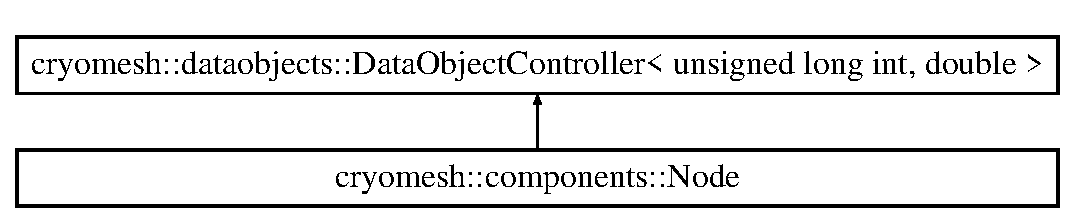
\includegraphics[height=2.000000cm]{classcryomesh_1_1components_1_1Node}
\end{center}
\end{figure}
\subsection*{\-Public \-Types}
\begin{DoxyCompactItemize}
\item 
enum \hyperlink{classcryomesh_1_1components_1_1Node_a291becdd589b5bd338d5c0dd28199798}{\-Activation\-State} \{ \hyperlink{classcryomesh_1_1components_1_1Node_a291becdd589b5bd338d5c0dd28199798af92c268dc627d5fed69c32d6f0d3d82e}{\-Positive}, 
\hyperlink{classcryomesh_1_1components_1_1Node_a291becdd589b5bd338d5c0dd28199798ab3953601aa3c39f46155bba156a29fb6}{\-Negative}, 
\hyperlink{classcryomesh_1_1components_1_1Node_a291becdd589b5bd338d5c0dd28199798a4b7d78598441d7b9fd51e7bb58415f4b}{\-None}
 \}
\begin{DoxyCompactList}\small\item\em \-Enum representing posible activation states. \end{DoxyCompactList}\item 
enum \hyperlink{classcryomesh_1_1components_1_1Node_adf36d853022d1b106766aefd3b9f3641}{\-Recovery\-Setting} \{ \hyperlink{classcryomesh_1_1components_1_1Node_adf36d853022d1b106766aefd3b9f3641a91a2a1e92850c99a22afb1574bd74574}{\-C\-L\-E\-A\-R\-\_\-\-A\-L\-L\-\_\-\-I\-M\-P\-U\-L\-S\-E\-S} =  1, 
\hyperlink{classcryomesh_1_1components_1_1Node_adf36d853022d1b106766aefd3b9f3641a000e55e803e043c412dfbc2d222a34e6}{\-C\-L\-E\-A\-R\-\_\-\-A\-C\-T\-I\-V\-E\-\_\-\-I\-M\-P\-U\-L\-S\-E\-S} =  2, 
\hyperlink{classcryomesh_1_1components_1_1Node_adf36d853022d1b106766aefd3b9f3641a3d8ee8e0f92053fa06eaa4184f1854b1}{\-D\-E\-A\-C\-T\-I\-V\-A\-T\-E\-\_\-\-D\-U\-R\-I\-N\-G\-\_\-\-R\-E\-C\-O\-V\-E\-R\-Y} =  4
 \}
\end{DoxyCompactItemize}
\subsection*{\-Public \-Member \-Functions}
\begin{DoxyCompactItemize}
\item 
\hyperlink{classcryomesh_1_1components_1_1Node_aa28b184629aa9412666b9674a10c45ab}{\-Node} ()
\begin{DoxyCompactList}\small\item\em \-Contructor. \end{DoxyCompactList}\item 
virtual \hyperlink{classcryomesh_1_1components_1_1Node_ae1ac5a2ed22ebc9b0cb7055b3e456097}{$\sim$\-Node} ()
\begin{DoxyCompactList}\small\item\em \-Destructor. \end{DoxyCompactList}\item 
virtual void \hyperlink{classcryomesh_1_1components_1_1Node_a960b083db047bb1b860d4ed09f9ad583}{update} ()
\item 
virtual void \hyperlink{classcryomesh_1_1components_1_1Node_ac40f33e5d0986d208b21302232f8a165}{force\-Fire} ()
\begin{DoxyCompactList}\small\item\em \-Force the node to fire. \end{DoxyCompactList}\item 
virtual boost\-::shared\-\_\-ptr\*
$<$ \hyperlink{classcryomesh_1_1components_1_1Impulse}{\-Impulse} $>$ \hyperlink{classcryomesh_1_1components_1_1Node_a1098a370eba39dce1388d657e3d3aef9}{add\-Impulse} (boost\-::shared\-\_\-ptr$<$ \hyperlink{classcryomesh_1_1components_1_1Impulse}{\-Impulse} $>$ impulse)
\begin{DoxyCompactList}\small\item\em \-Add incoming \hyperlink{classcryomesh_1_1components_1_1Impulse}{\-Impulse}. \end{DoxyCompactList}\item 
virtual void \hyperlink{classcryomesh_1_1components_1_1Node_af8ab49ec82ff876549f75123d65c41b4}{add\-Impulses} (std\-::list$<$ boost\-::shared\-\_\-ptr$<$ \hyperlink{classcryomesh_1_1components_1_1Impulse}{\-Impulse} $>$ $>$ \hyperlink{classcryomesh_1_1components_1_1Node_a8e9ae8373052bb63f2f1e6e453a3c18d}{impulses})
\begin{DoxyCompactList}\small\item\em \-Add a list of incoming \-Impulses. \end{DoxyCompactList}\item 
const \hyperlink{classcryomesh_1_1common_1_1Connector}{common\-::\-Connector}$<$ \hyperlink{classcryomesh_1_1components_1_1Node}{\-Node}, \*
\hyperlink{classcryomesh_1_1components_1_1Connection}{\-Connection} $>$ \& \hyperlink{classcryomesh_1_1components_1_1Node_a28367d5dc76da04958ca22f6384f6073}{get\-Connector} () const 
\begin{DoxyCompactList}\small\item\em \-Get the \-Connector object for this \hyperlink{classcryomesh_1_1components_1_1Node}{\-Node}. \end{DoxyCompactList}\item 
\hyperlink{classcryomesh_1_1common_1_1Connector}{common\-::\-Connector}$<$ \hyperlink{classcryomesh_1_1components_1_1Node}{\-Node}, \*
\hyperlink{classcryomesh_1_1components_1_1Connection}{\-Connection} $>$ \& \hyperlink{classcryomesh_1_1components_1_1Node_ae28261bb67b7412a67b21a4e4adaa9b1}{get\-Mutable\-Connector} ()
\begin{DoxyCompactList}\small\item\em \-Get the mutable \-Connector object for this \hyperlink{classcryomesh_1_1components_1_1Node}{\-Node}. \end{DoxyCompactList}\item 
bool \hyperlink{classcryomesh_1_1components_1_1Node_a501c4e986a566a4e7fc5f9c87e9c4d8e}{is\-Input\-Isolated} () const 
\item 
bool \hyperlink{classcryomesh_1_1components_1_1Node_a211678e84d71cb71e3721eb9725fa934}{is\-Output\-Isolated} () const 
\item 
void \hyperlink{classcryomesh_1_1components_1_1Node_a4a7775d987020170538f059688ff4a1f}{connect\-Input} (boost\-::shared\-\_\-ptr$<$ \hyperlink{classcryomesh_1_1components_1_1Connection}{\-Connection} $>$ con)
\item 
void \hyperlink{classcryomesh_1_1components_1_1Node_a660adcc4e2b3b7a427ad4625e5279de4}{connect\-Output} (boost\-::shared\-\_\-ptr$<$ \hyperlink{classcryomesh_1_1components_1_1Connection}{\-Connection} $>$ con)
\item 
const \hyperlink{classcryomesh_1_1components_1_1ImpulseCollection}{\-Impulse\-Collection} \& \hyperlink{classcryomesh_1_1components_1_1Node_a63316f8a1ad0ffe3ee22f8b455ef27a4}{get\-Impulses} () const 
\begin{DoxyCompactList}\small\item\em \-Get the collection of \-Impulses for this \hyperlink{classcryomesh_1_1components_1_1Node}{\-Node}. \end{DoxyCompactList}\item 
const boost\-::shared\-\_\-ptr$<$ \hyperlink{classcryomesh_1_1components_1_1Impulse}{\-Impulse} $>$ \hyperlink{classcryomesh_1_1components_1_1Node_a8a90b1faf2e6b633bbb4853e522c29b7}{get\-Emitted\-Impulse} () const 
\begin{DoxyCompactList}\small\item\em \-Get the \hyperlink{classcryomesh_1_1components_1_1Impulse}{\-Impulse} that is emitted. \end{DoxyCompactList}\item 
boost\-::shared\-\_\-ptr$<$ \hyperlink{classcryomesh_1_1components_1_1Impulse}{\-Impulse} $>$ \hyperlink{classcryomesh_1_1components_1_1Node_aa6e0c0a0063e657053482aac777759d3}{get\-Mutable\-Emitted\-Impulse} ()
\begin{DoxyCompactList}\small\item\em \-Get the mutable \hyperlink{classcryomesh_1_1components_1_1Impulse}{\-Impulse} that is emitted. \end{DoxyCompactList}\item 
virtual void \hyperlink{classcryomesh_1_1components_1_1Node_a8fc7efcfff86d2ca72b54166f600b7d0}{emit\-Impulse\-Positive} ()
\begin{DoxyCompactList}\small\item\em \-Emit a positive impulse to outgoing connections. \end{DoxyCompactList}\item 
virtual void \hyperlink{classcryomesh_1_1components_1_1Node_a75addf25b1b16bf1476cf19f00d7513d}{emit\-Impulse\-Negative} ()
\begin{DoxyCompactList}\small\item\em \-Emit a negative impulse to outgoing connections. \end{DoxyCompactList}\item 
\hyperlink{classcryomesh_1_1components_1_1ImpulseCollection}{\-Impulse\-Collection} \& \hyperlink{classcryomesh_1_1components_1_1Node_adaa0b9f4c9a6130525fce2e43f418bc3}{get\-Mutable\-Impulses} ()
\begin{DoxyCompactList}\small\item\em \-Get the mutable collection of \-Impulses for this \hyperlink{classcryomesh_1_1components_1_1Node}{\-Node}. \end{DoxyCompactList}\item 
const std\-::map$<$ \hyperlink{classcryomesh_1_1common_1_1Cycle}{common\-::\-Cycle}, \*
double $>$ \& \hyperlink{classcryomesh_1_1components_1_1Node_a98801c702bf6613f06880f7cc577ddd7}{get\-Activities} () const 
\begin{DoxyCompactList}\small\item\em \-Get the collection of all activities. \end{DoxyCompactList}\item 
double \hyperlink{classcryomesh_1_1components_1_1Node_ab9f3406d26f50f3dcee4b19c30cfc893}{update\-Activity} ()
\begin{DoxyCompactList}\small\item\em \-Update and get the current activity of the node. \end{DoxyCompactList}\item 
double \hyperlink{classcryomesh_1_1components_1_1Node_a2074cbfe458cda6fc10997ae6965f168}{update\-Activity} (const \hyperlink{classcryomesh_1_1common_1_1Cycle}{common\-::\-Cycle} \&cycle)
\begin{DoxyCompactList}\small\item\em \-Update and get the activity of the node on specific cycle. \end{DoxyCompactList}\item 
double \hyperlink{classcryomesh_1_1components_1_1Node_a355e414f9a353883fd0f4b7cae24d6cc}{get\-Activity} () const 
\begin{DoxyCompactList}\small\item\em \-Get the current activity of the node. \end{DoxyCompactList}\item 
double \hyperlink{classcryomesh_1_1components_1_1Node_a07c29936e9a695e32365708f8c381456}{get\-Activity} (const \hyperlink{classcryomesh_1_1common_1_1Cycle}{common\-::\-Cycle} \&cycle) const 
\begin{DoxyCompactList}\small\item\em \-Get the activity of the node on specific cycle. \end{DoxyCompactList}\item 
double \hyperlink{classcryomesh_1_1components_1_1Node_ab561d1b0b10339ad8ae2280a8063677b}{get\-Activity\-Threshold} () const 
\item 
double \hyperlink{classcryomesh_1_1components_1_1Node_acf3b0de410fee4350390bd527c544187}{set\-Activity} (double activity)
\begin{DoxyCompactList}\small\item\em \-Set the current activity of the node. \end{DoxyCompactList}\item 
double \hyperlink{classcryomesh_1_1components_1_1Node_aacac1b5adbafe83a7dcae288a607ee31}{set\-Activity} (const \hyperlink{classcryomesh_1_1common_1_1Cycle}{common\-::\-Cycle} \&cycle, double activity)
\begin{DoxyCompactList}\small\item\em \-Set the activity at cycle of the node. \end{DoxyCompactList}\item 
boost\-::shared\-\_\-ptr\*
$<$ \hyperlink{classcryomesh_1_1manager_1_1DatabaseObject}{manager\-::\-Database\-Object} $>$ \hyperlink{classcryomesh_1_1components_1_1Node_a811e64601504ff99536c2680429c7582}{get\-Database\-Object} () const 
\begin{DoxyCompactList}\small\item\em \-Return a database object for this node. \end{DoxyCompactList}\item 
const spacial\-::\-Point \& \hyperlink{classcryomesh_1_1components_1_1Node_a313531f48e1ccc3902fdeb313d41bd7b}{get\-Position} () const 
\begin{DoxyCompactList}\small\item\em get the position of the node \end{DoxyCompactList}\item 
void \hyperlink{classcryomesh_1_1components_1_1Node_a970e8e8ae18053bd9e087ce7faf720de}{set\-Position} (const spacial\-::\-Point \&new\-\_\-position)
\begin{DoxyCompactList}\small\item\em \-Set the spacial position of the node, remembering to update connections lengths. \end{DoxyCompactList}\item 
\hyperlink{classcryomesh_1_1components_1_1Node_a291becdd589b5bd338d5c0dd28199798}{\-Activation\-State} \hyperlink{classcryomesh_1_1components_1_1Node_ac0f6e2c8823c98dc3d85091b2deef3f7}{get\-Last\-Activation\-State} () const 
\begin{DoxyCompactList}\small\item\em \-Get the last activation state. \end{DoxyCompactList}\item 
void \hyperlink{classcryomesh_1_1components_1_1Node_a5ec290205a68a8635a740ae32608cebf}{randomise} ()
\begin{DoxyCompactList}\small\item\em \-Randomise the nodes state. \end{DoxyCompactList}\item 
virtual void \hyperlink{classcryomesh_1_1components_1_1Node_a42acc61b6b0d590433215535d3bc67cd}{enable\-Debug} (bool b)
\item 
bool \hyperlink{classcryomesh_1_1components_1_1Node_a83303fef90a3093807d76a59e4df5288}{is\-Triggered} (\hyperlink{classcryomesh_1_1components_1_1Node_a291becdd589b5bd338d5c0dd28199798}{\-Activation\-State} state=\hyperlink{classcryomesh_1_1components_1_1Node_a291becdd589b5bd338d5c0dd28199798a4b7d78598441d7b9fd51e7bb58415f4b}{\-None})
\begin{DoxyCompactList}\small\item\em \-Check if \hyperlink{classcryomesh_1_1components_1_1Node}{\-Node} is currently triggered. \end{DoxyCompactList}\item 
bool \hyperlink{classcryomesh_1_1components_1_1Node_af2943ca887ce9c2b1a65297cae14d752}{is\-Active} (const \hyperlink{classcryomesh_1_1components_1_1Node_a291becdd589b5bd338d5c0dd28199798}{\-Activation\-State} state=\hyperlink{classcryomesh_1_1components_1_1Node_a291becdd589b5bd338d5c0dd28199798a4b7d78598441d7b9fd51e7bb58415f4b}{\-None})
\begin{DoxyCompactList}\small\item\em \-Check if \hyperlink{classcryomesh_1_1components_1_1Node}{\-Node} is currently activated. \end{DoxyCompactList}\item 
bool \hyperlink{classcryomesh_1_1components_1_1Node_a2309ba6b3ffa640410dfdc1630a66400}{is\-Live} ()
\begin{DoxyCompactList}\small\item\em \-Check if \hyperlink{classcryomesh_1_1components_1_1Node}{\-Node} is live, ie active at any point in now or the future. \end{DoxyCompactList}\item 
void \hyperlink{classcryomesh_1_1components_1_1Node_ade4a1e563ab60b7d8ff8fa6830d2fcbf}{destroy\-All\-Connections} ()
\begin{DoxyCompactList}\small\item\em \-Destroy all connections. \end{DoxyCompactList}\item 
void \hyperlink{classcryomesh_1_1components_1_1Node_ad61b50a382ae7d64cedb8f8f8a5d66cd}{destroy\-All\-Input\-Connections} ()
\begin{DoxyCompactList}\small\item\em \-Destroy \-Input connections by removing them all from both their attached input and output nodes. \end{DoxyCompactList}\item 
void \hyperlink{classcryomesh_1_1components_1_1Node_a8147d9a370a680ffb6c847a0df276114}{destroy\-All\-Output\-Connections} ()
\begin{DoxyCompactList}\small\item\em \-Destroy \-Output connections by removing them all from both their attached input and output nodes. \end{DoxyCompactList}\item 
bool \hyperlink{classcryomesh_1_1components_1_1Node_a2f55aa5adcac4a2f1aa1f0a7c8fc697d}{is\-Primary\-Input\-Attached\-Node} () const 
\item 
bool \hyperlink{classcryomesh_1_1components_1_1Node_a8466a252c7a4e6fb2d825826be53e218}{is\-Primary\-Output\-Attached\-Node} () const 
\item 
std\-::vector$<$ boost\-::shared\-\_\-ptr\*
$<$ \hyperlink{classcryomesh_1_1components_1_1Connection}{\-Connection} $>$ $>$ \hyperlink{classcryomesh_1_1components_1_1Node_a0f172d0f98de3d008d2d0a5efa15d3b2}{get\-Primary\-Input\-Connections} ()
\item 
std\-::vector$<$ boost\-::shared\-\_\-ptr\*
$<$ \hyperlink{classcryomesh_1_1components_1_1Connection}{\-Connection} $>$ $>$ \hyperlink{classcryomesh_1_1components_1_1Node_aa0ac6ca5e0d98261840760bdc07e4d3f}{get\-Primary\-Output\-Connections} ()
\item 
std\-::ostream \& \hyperlink{classcryomesh_1_1components_1_1Node_a036878d7028df14d1015c0ce413d4038}{print\-Connections} (std\-::ostream \&os, const std\-::map$<$ boost\-::uuids\-::uuid, boost\-::shared\-\_\-ptr$<$ \hyperlink{classcryomesh_1_1components_1_1Connection}{\-Connection} $>$ $>$ \&all\-\_\-cons, const std\-::string formatter=\char`\"{}\char`\"{}) const 
\item 
virtual void \hyperlink{classcryomesh_1_1dataobjects_1_1DataObjectController_a3e510413675407ec0a6745345ca9a3a8}{enable\-Logging} (bool enable)
\begin{DoxyCompactList}\small\item\em \-Whether logging is enabled or not. \end{DoxyCompactList}\item 
virtual const std\-::map\*
$<$ unsigned long int, double $>$ \& \hyperlink{classcryomesh_1_1dataobjects_1_1DataObjectController_a70a03ee28392ecf2e039702a18511f05}{get\-Map} ()
\begin{DoxyCompactList}\small\item\em \-Get all cycle values. \end{DoxyCompactList}\item 
virtual const \*
\hyperlink{classcryomesh_1_1dataobjects_1_1DataObject}{dataobjects\-::\-Data\-Object}\*
$<$ unsigned long int, double $>$ \& \hyperlink{classcryomesh_1_1dataobjects_1_1DataObjectController_aa919e8676a611028c6b6e6791c87f438}{get\-Data\-Object} ()
\begin{DoxyCompactList}\small\item\em \-Get data object. \end{DoxyCompactList}\item 
virtual void \hyperlink{classcryomesh_1_1dataobjects_1_1DataObjectController_ae015efe3d10cced82d5043f560cbe04f}{refresh\-Data\-Object} ()
\begin{DoxyCompactList}\small\item\em \-Function to allow refreshing implementation if required by subclasses. \end{DoxyCompactList}\end{DoxyCompactItemize}
\subsection*{\-Static \-Public \-Member \-Functions}
\begin{DoxyCompactItemize}
\item 
static boost\-::shared\-\_\-ptr$<$ \hyperlink{classcryomesh_1_1components_1_1Node}{\-Node} $>$ \hyperlink{classcryomesh_1_1components_1_1Node_a3ffbf4f53801b9e83c815e97e3072302}{get\-Random} (const spacial\-::\-Point \&max\-\_\-point=\hyperlink{classcryomesh_1_1components_1_1Node_a3f4f3b7d2bba533fc0487b4f10c1efcd}{\-M\-A\-X\-\_\-\-B\-O\-U\-N\-D\-I\-N\-G\-\_\-\-B\-O\-X\-\_\-\-P\-O\-I\-N\-T})
\end{DoxyCompactItemize}
\subsection*{\-Static \-Public \-Attributes}
\begin{DoxyCompactItemize}
\item 
static const int \hyperlink{classcryomesh_1_1components_1_1Node_ae5b4fa1289a3ab819710ff7a40a77282}{\-M\-A\-X\-\_\-\-A\-C\-T\-I\-V\-I\-T\-I\-E\-S\-\_\-\-L\-E\-N\-G\-T\-H} = 10
\item 
static const double \hyperlink{classcryomesh_1_1components_1_1Node_adcfc8e07f6d216817a45f1c27190967b}{\-M\-A\-X\-\_\-\-A\-C\-T\-I\-V\-I\-T\-Y\-\_\-\-T\-H\-R\-E\-S\-H\-O\-L\-D} = 3 $\ast$ \hyperlink{classcryomesh_1_1components_1_1Impulse_af8e9eb795f1ea3cef81d6afeb7166ad2}{\-Impulse\-::\-M\-A\-X\-\_\-\-A\-C\-T\-I\-V\-I\-T\-Y}
\item 
static const double \hyperlink{classcryomesh_1_1components_1_1Node_a5ed72f665cf7b32914e61b4655bd52ca}{\-M\-I\-N\-\_\-\-A\-C\-T\-I\-V\-I\-T\-Y\-\_\-\-T\-H\-R\-E\-S\-H\-O\-L\-D} = 1 $\ast$ \hyperlink{classcryomesh_1_1components_1_1Impulse_af8e9eb795f1ea3cef81d6afeb7166ad2}{\-Impulse\-::\-M\-A\-X\-\_\-\-A\-C\-T\-I\-V\-I\-T\-Y}
\item 
static const spacial\-::\-Point \hyperlink{classcryomesh_1_1components_1_1Node_a3f4f3b7d2bba533fc0487b4f10c1efcd}{\-M\-A\-X\-\_\-\-B\-O\-U\-N\-D\-I\-N\-G\-\_\-\-B\-O\-X\-\_\-\-P\-O\-I\-N\-T} = spacial\-::\-Point(100, 100, 100)
\end{DoxyCompactItemize}
\subsection*{\-Protected \-Member \-Functions}
\begin{DoxyCompactItemize}
\item 
virtual \hyperlink{classcryomesh_1_1components_1_1Node_a291becdd589b5bd338d5c0dd28199798}{\-Node\-::\-Activation\-State} \hyperlink{classcryomesh_1_1components_1_1Node_adeebae01197045204f1b9cda1ece3372}{check\-Activation\-State} ()
\begin{DoxyCompactList}\small\item\em \-Check level of impulses and decide whether to activate the node. \end{DoxyCompactList}\item 
virtual \hyperlink{classcryomesh_1_1components_1_1Node_a291becdd589b5bd338d5c0dd28199798}{\-Node\-::\-Activation\-State} \hyperlink{classcryomesh_1_1components_1_1Node_ac4f969b7c236a6e910031101879c8da3}{check\-Fire} ()
\begin{DoxyCompactList}\small\item\em \-Check if the object is ready to fire off an impulse and carry it out. \end{DoxyCompactList}\item 
virtual void \hyperlink{classcryomesh_1_1components_1_1Node_ade03584e4db3f8e1eeddc9ad371b4658}{update\-Impulses} ()
\begin{DoxyCompactList}\small\item\em \-Update the collection of impulses by one cycle. \end{DoxyCompactList}\item 
virtual void \hyperlink{classcryomesh_1_1components_1_1Node_a3323a7f7e9958b78552746ddf374c4fc}{emit\-Impulse} (bool positive)
\begin{DoxyCompactList}\small\item\em \-Emit an impulse to outgoing connections. \end{DoxyCompactList}\item 
virtual double \hyperlink{classcryomesh_1_1components_1_1Node_ab916e0beff2dcecd14c284dd63bd0585}{add\-Activity} (\hyperlink{classcryomesh_1_1common_1_1Cycle}{common\-::\-Cycle}, double activity)
\begin{DoxyCompactList}\small\item\em \-Add an activity to the list of activities. \end{DoxyCompactList}\item 
virtual void \hyperlink{classcryomesh_1_1components_1_1Node_ab769e1efe1fd3e0ae9ff0a7643dd473c}{update\-Position} ()
\begin{DoxyCompactList}\small\item\em \-Recalculate state of node and connections based on current position. \end{DoxyCompactList}\item 
virtual void \hyperlink{classcryomesh_1_1components_1_1Node_a92bbb37859ba4b810381bd733ad5d63c}{enter\-Recovery} (const int recovery\-\_\-settings=\hyperlink{classcryomesh_1_1components_1_1Node_adf36d853022d1b106766aefd3b9f3641a91a2a1e92850c99a22afb1574bd74574}{\-C\-L\-E\-A\-R\-\_\-\-A\-L\-L\-\_\-\-I\-M\-P\-U\-L\-S\-E\-S})
\end{DoxyCompactItemize}
\subsection*{\-Protected \-Attributes}
\begin{DoxyCompactItemize}
\item 
\hyperlink{classcryomesh_1_1dataobjects_1_1DataObject}{dataobjects\-::\-Data\-Object}\*
$<$ unsigned long int, double $>$ \hyperlink{classcryomesh_1_1dataobjects_1_1DataObjectController_aa13d30e9fa2f1caa0510635214d4bb26}{data\-Object}
\end{DoxyCompactItemize}
\subsection*{\-Private \-Attributes}
\begin{DoxyCompactItemize}
\item 
double \hyperlink{classcryomesh_1_1components_1_1Node_a270451d7286a4e6f344559a3d48d1193}{activity\-Threshold}
\item 
boost\-::shared\-\_\-ptr\*
$<$ \hyperlink{classcryomesh_1_1common_1_1Connector}{common\-::\-Connector}$<$ \hyperlink{classcryomesh_1_1components_1_1Node}{\-Node}, \*
\hyperlink{classcryomesh_1_1components_1_1Connection}{\-Connection} $>$ $>$ \hyperlink{classcryomesh_1_1components_1_1Node_a43b68f9f1a83bca4d4fc4f55bb8dd8de}{connector}
\item 
\hyperlink{classcryomesh_1_1components_1_1ImpulseCollection}{\-Impulse\-Collection} \hyperlink{classcryomesh_1_1components_1_1Node_a8e9ae8373052bb63f2f1e6e453a3c18d}{impulses}
\item 
boost\-::shared\-\_\-ptr$<$ \hyperlink{classcryomesh_1_1components_1_1Impulse}{\-Impulse} $>$ \hyperlink{classcryomesh_1_1components_1_1Node_a6b5e004fc2bbdbd8ec7173b44af8ffe5}{emitted\-Impulse}
\item 
\hyperlink{classcryomesh_1_1dataobjects_1_1DataObject}{dataobjects\-::\-Data\-Object}\*
$<$ \hyperlink{classcryomesh_1_1common_1_1Cycle}{common\-::\-Cycle}, double $>$ \hyperlink{classcryomesh_1_1components_1_1Node_a39bf3a9c006d8ee03769d6b86127e7cf}{activities}
\item 
spacial\-::\-Point \hyperlink{classcryomesh_1_1components_1_1Node_afad345a6d8cc1eacc555acde8c065b61}{position}
\item 
\hyperlink{classcryomesh_1_1components_1_1Node_a291becdd589b5bd338d5c0dd28199798}{\-Activation\-State} \hyperlink{classcryomesh_1_1components_1_1Node_ab94a09be9e58cc248f9d62ed5c45c83d}{last\-Activation\-State}
\end{DoxyCompactItemize}
\subsection*{\-Friends}
\begin{DoxyCompactItemize}
\item 
std\-::ostream \& \hyperlink{classcryomesh_1_1components_1_1Node_aa13c716dda529b01000661b942327bd6}{operator$<$$<$} (std\-::ostream \&os, const \hyperlink{classcryomesh_1_1components_1_1Node}{\-Node} \&obj)
\begin{DoxyCompactList}\small\item\em \-To stream operator. \end{DoxyCompactList}\end{DoxyCompactItemize}


\subsection{\-Detailed \-Description}
\hyperlink{classcryomesh_1_1components_1_1Node}{\-Node} is an accumulation and computational nodal point of impulses. 

\-A \hyperlink{classcryomesh_1_1components_1_1Node}{\-Node} represents the end point of one or many connections. \-Here, \-Impulses are accumulated and new \-Impulses generated depending on some determining criteria 

\-Definition at line 38 of file \-Node.\-h.



\subsection{\-Member \-Enumeration \-Documentation}
\hypertarget{classcryomesh_1_1components_1_1Node_a291becdd589b5bd338d5c0dd28199798}{\index{cryomesh\-::components\-::\-Node@{cryomesh\-::components\-::\-Node}!\-Activation\-State@{\-Activation\-State}}
\index{\-Activation\-State@{\-Activation\-State}!cryomesh::components::Node@{cryomesh\-::components\-::\-Node}}
\subsubsection[{\-Activation\-State}]{\setlength{\rightskip}{0pt plus 5cm}enum {\bf cryomesh\-::components\-::\-Node\-::\-Activation\-State}}}\label{classcryomesh_1_1components_1_1Node_a291becdd589b5bd338d5c0dd28199798}


\-Enum representing posible activation states. 

\-Last activation state. \begin{Desc}
\item[\-Enumerator\-: ]\par
\begin{description}
\index{\-Positive@{\-Positive}!cryomesh\-::components\-::\-Node@{cryomesh\-::components\-::\-Node}}\index{cryomesh\-::components\-::\-Node@{cryomesh\-::components\-::\-Node}!\-Positive@{\-Positive}}\item[{\em 
\hypertarget{classcryomesh_1_1components_1_1Node_a291becdd589b5bd338d5c0dd28199798af92c268dc627d5fed69c32d6f0d3d82e}{\-Positive}\label{classcryomesh_1_1components_1_1Node_a291becdd589b5bd338d5c0dd28199798af92c268dc627d5fed69c32d6f0d3d82e}
}]\index{\-Negative@{\-Negative}!cryomesh\-::components\-::\-Node@{cryomesh\-::components\-::\-Node}}\index{cryomesh\-::components\-::\-Node@{cryomesh\-::components\-::\-Node}!\-Negative@{\-Negative}}\item[{\em 
\hypertarget{classcryomesh_1_1components_1_1Node_a291becdd589b5bd338d5c0dd28199798ab3953601aa3c39f46155bba156a29fb6}{\-Negative}\label{classcryomesh_1_1components_1_1Node_a291becdd589b5bd338d5c0dd28199798ab3953601aa3c39f46155bba156a29fb6}
}]\index{\-None@{\-None}!cryomesh\-::components\-::\-Node@{cryomesh\-::components\-::\-Node}}\index{cryomesh\-::components\-::\-Node@{cryomesh\-::components\-::\-Node}!\-None@{\-None}}\item[{\em 
\hypertarget{classcryomesh_1_1components_1_1Node_a291becdd589b5bd338d5c0dd28199798a4b7d78598441d7b9fd51e7bb58415f4b}{\-None}\label{classcryomesh_1_1components_1_1Node_a291becdd589b5bd338d5c0dd28199798a4b7d78598441d7b9fd51e7bb58415f4b}
}]\end{description}
\end{Desc}



\-Definition at line 45 of file \-Node.\-h.

\hypertarget{classcryomesh_1_1components_1_1Node_adf36d853022d1b106766aefd3b9f3641}{\index{cryomesh\-::components\-::\-Node@{cryomesh\-::components\-::\-Node}!\-Recovery\-Setting@{\-Recovery\-Setting}}
\index{\-Recovery\-Setting@{\-Recovery\-Setting}!cryomesh::components::Node@{cryomesh\-::components\-::\-Node}}
\subsubsection[{\-Recovery\-Setting}]{\setlength{\rightskip}{0pt plus 5cm}enum {\bf cryomesh\-::components\-::\-Node\-::\-Recovery\-Setting}}}\label{classcryomesh_1_1components_1_1Node_adf36d853022d1b106766aefd3b9f3641}
\begin{Desc}
\item[\-Enumerator\-: ]\par
\begin{description}
\index{\-C\-L\-E\-A\-R\-\_\-\-A\-L\-L\-\_\-\-I\-M\-P\-U\-L\-S\-E\-S@{\-C\-L\-E\-A\-R\-\_\-\-A\-L\-L\-\_\-\-I\-M\-P\-U\-L\-S\-E\-S}!cryomesh\-::components\-::\-Node@{cryomesh\-::components\-::\-Node}}\index{cryomesh\-::components\-::\-Node@{cryomesh\-::components\-::\-Node}!\-C\-L\-E\-A\-R\-\_\-\-A\-L\-L\-\_\-\-I\-M\-P\-U\-L\-S\-E\-S@{\-C\-L\-E\-A\-R\-\_\-\-A\-L\-L\-\_\-\-I\-M\-P\-U\-L\-S\-E\-S}}\item[{\em 
\hypertarget{classcryomesh_1_1components_1_1Node_adf36d853022d1b106766aefd3b9f3641a91a2a1e92850c99a22afb1574bd74574}{\-C\-L\-E\-A\-R\-\_\-\-A\-L\-L\-\_\-\-I\-M\-P\-U\-L\-S\-E\-S}\label{classcryomesh_1_1components_1_1Node_adf36d853022d1b106766aefd3b9f3641a91a2a1e92850c99a22afb1574bd74574}
}]\index{\-C\-L\-E\-A\-R\-\_\-\-A\-C\-T\-I\-V\-E\-\_\-\-I\-M\-P\-U\-L\-S\-E\-S@{\-C\-L\-E\-A\-R\-\_\-\-A\-C\-T\-I\-V\-E\-\_\-\-I\-M\-P\-U\-L\-S\-E\-S}!cryomesh\-::components\-::\-Node@{cryomesh\-::components\-::\-Node}}\index{cryomesh\-::components\-::\-Node@{cryomesh\-::components\-::\-Node}!\-C\-L\-E\-A\-R\-\_\-\-A\-C\-T\-I\-V\-E\-\_\-\-I\-M\-P\-U\-L\-S\-E\-S@{\-C\-L\-E\-A\-R\-\_\-\-A\-C\-T\-I\-V\-E\-\_\-\-I\-M\-P\-U\-L\-S\-E\-S}}\item[{\em 
\hypertarget{classcryomesh_1_1components_1_1Node_adf36d853022d1b106766aefd3b9f3641a000e55e803e043c412dfbc2d222a34e6}{\-C\-L\-E\-A\-R\-\_\-\-A\-C\-T\-I\-V\-E\-\_\-\-I\-M\-P\-U\-L\-S\-E\-S}\label{classcryomesh_1_1components_1_1Node_adf36d853022d1b106766aefd3b9f3641a000e55e803e043c412dfbc2d222a34e6}
}]\index{\-D\-E\-A\-C\-T\-I\-V\-A\-T\-E\-\_\-\-D\-U\-R\-I\-N\-G\-\_\-\-R\-E\-C\-O\-V\-E\-R\-Y@{\-D\-E\-A\-C\-T\-I\-V\-A\-T\-E\-\_\-\-D\-U\-R\-I\-N\-G\-\_\-\-R\-E\-C\-O\-V\-E\-R\-Y}!cryomesh\-::components\-::\-Node@{cryomesh\-::components\-::\-Node}}\index{cryomesh\-::components\-::\-Node@{cryomesh\-::components\-::\-Node}!\-D\-E\-A\-C\-T\-I\-V\-A\-T\-E\-\_\-\-D\-U\-R\-I\-N\-G\-\_\-\-R\-E\-C\-O\-V\-E\-R\-Y@{\-D\-E\-A\-C\-T\-I\-V\-A\-T\-E\-\_\-\-D\-U\-R\-I\-N\-G\-\_\-\-R\-E\-C\-O\-V\-E\-R\-Y}}\item[{\em 
\hypertarget{classcryomesh_1_1components_1_1Node_adf36d853022d1b106766aefd3b9f3641a3d8ee8e0f92053fa06eaa4184f1854b1}{\-D\-E\-A\-C\-T\-I\-V\-A\-T\-E\-\_\-\-D\-U\-R\-I\-N\-G\-\_\-\-R\-E\-C\-O\-V\-E\-R\-Y}\label{classcryomesh_1_1components_1_1Node_adf36d853022d1b106766aefd3b9f3641a3d8ee8e0f92053fa06eaa4184f1854b1}
}]\end{description}
\end{Desc}



\-Definition at line 49 of file \-Node.\-h.



\subsection{\-Constructor \& \-Destructor \-Documentation}
\hypertarget{classcryomesh_1_1components_1_1Node_aa28b184629aa9412666b9674a10c45ab}{\index{cryomesh\-::components\-::\-Node@{cryomesh\-::components\-::\-Node}!\-Node@{\-Node}}
\index{\-Node@{\-Node}!cryomesh::components::Node@{cryomesh\-::components\-::\-Node}}
\subsubsection[{\-Node}]{\setlength{\rightskip}{0pt plus 5cm}{\bf cryomesh\-::components\-::\-Node\-::\-Node} (
\begin{DoxyParamCaption}
{}
\end{DoxyParamCaption}
)}}\label{classcryomesh_1_1components_1_1Node_aa28b184629aa9412666b9674a10c45ab}


\-Contructor. 

\-Contructor for \hyperlink{classcryomesh_1_1components_1_1Node}{\-Node} 

\-Definition at line 37 of file \-Node.\-cpp.



\-References activities, connector, emitted\-Impulse, \-M\-A\-X\-\_\-\-A\-C\-T\-I\-V\-I\-T\-I\-E\-S\-\_\-\-L\-E\-N\-G\-T\-H, and cryomesh\-::dataobjects\-::\-Data\-Object$<$ U, T $>$\-::set\-Dataset\-Maximum\-Size().

\hypertarget{classcryomesh_1_1components_1_1Node_ae1ac5a2ed22ebc9b0cb7055b3e456097}{\index{cryomesh\-::components\-::\-Node@{cryomesh\-::components\-::\-Node}!$\sim$\-Node@{$\sim$\-Node}}
\index{$\sim$\-Node@{$\sim$\-Node}!cryomesh::components::Node@{cryomesh\-::components\-::\-Node}}
\subsubsection[{$\sim$\-Node}]{\setlength{\rightskip}{0pt plus 5cm}{\bf cryomesh\-::components\-::\-Node\-::$\sim$\-Node} (
\begin{DoxyParamCaption}
{}
\end{DoxyParamCaption}
)\hspace{0.3cm}{\ttfamily  \mbox{[}virtual\mbox{]}}}}\label{classcryomesh_1_1components_1_1Node_ae1ac5a2ed22ebc9b0cb7055b3e456097}


\-Destructor. 

\-Destructor for \hyperlink{classcryomesh_1_1components_1_1Node}{\-Node} 

\-Definition at line 46 of file \-Node.\-cpp.



\subsection{\-Member \-Function \-Documentation}
\hypertarget{classcryomesh_1_1components_1_1Node_ab916e0beff2dcecd14c284dd63bd0585}{\index{cryomesh\-::components\-::\-Node@{cryomesh\-::components\-::\-Node}!add\-Activity@{add\-Activity}}
\index{add\-Activity@{add\-Activity}!cryomesh::components::Node@{cryomesh\-::components\-::\-Node}}
\subsubsection[{add\-Activity}]{\setlength{\rightskip}{0pt plus 5cm}double {\bf cryomesh\-::components\-::\-Node\-::add\-Activity} (
\begin{DoxyParamCaption}
\item[{{\bf common\-::\-Cycle}}]{cycle, }
\item[{double}]{activity}
\end{DoxyParamCaption}
)\hspace{0.3cm}{\ttfamily  \mbox{[}protected, virtual\mbox{]}}}}\label{classcryomesh_1_1components_1_1Node_ab916e0beff2dcecd14c284dd63bd0585}


\-Add an activity to the list of activities. 


\begin{DoxyParams}{\-Parameters}
{\em \-Cycle} & cycle \-The cycle this activity is on \\
\hline
{\em double} & activity \-The activity to add\\
\hline
\end{DoxyParams}
\begin{DoxyReturn}{\-Returns}
\-The current activity 
\end{DoxyReturn}


\-Definition at line 291 of file \-Node.\-cpp.



\-References activities, and cryomesh\-::dataobjects\-::\-Data\-Object$<$ U, T $>$\-::insert().



\-Referenced by set\-Activity().

\hypertarget{classcryomesh_1_1components_1_1Node_a1098a370eba39dce1388d657e3d3aef9}{\index{cryomesh\-::components\-::\-Node@{cryomesh\-::components\-::\-Node}!add\-Impulse@{add\-Impulse}}
\index{add\-Impulse@{add\-Impulse}!cryomesh::components::Node@{cryomesh\-::components\-::\-Node}}
\subsubsection[{add\-Impulse}]{\setlength{\rightskip}{0pt plus 5cm}boost\-::shared\-\_\-ptr$<$ {\bf \-Impulse} $>$ {\bf cryomesh\-::components\-::\-Node\-::add\-Impulse} (
\begin{DoxyParamCaption}
\item[{boost\-::shared\-\_\-ptr$<$ {\bf \-Impulse} $>$}]{impulse}
\end{DoxyParamCaption}
)\hspace{0.3cm}{\ttfamily  \mbox{[}virtual\mbox{]}}}}\label{classcryomesh_1_1components_1_1Node_a1098a370eba39dce1388d657e3d3aef9}


\-Add incoming \hyperlink{classcryomesh_1_1components_1_1Impulse}{\-Impulse}. 


\begin{DoxyParams}{\-Parameters}
{\em boost\-::shared\-\_\-ptr$<$\-Impulse$>$} & impulse \-The \hyperlink{classcryomesh_1_1components_1_1Impulse}{\-Impulse} to add \\
\hline
\end{DoxyParams}
\begin{DoxyReturn}{\-Returns}
boost\-::shared\-\_\-ptr$<$\-Impulse$>$ \-The impulse added, null if none added 
\end{DoxyReturn}


\-Definition at line 141 of file \-Node.\-cpp.



\-References get\-Mutable\-Impulses(), and cryomesh\-::common\-::\-Time\-Keeper\-::get\-Time\-Keeper().



\-Referenced by add\-Impulses(), and force\-Fire().

\hypertarget{classcryomesh_1_1components_1_1Node_af8ab49ec82ff876549f75123d65c41b4}{\index{cryomesh\-::components\-::\-Node@{cryomesh\-::components\-::\-Node}!add\-Impulses@{add\-Impulses}}
\index{add\-Impulses@{add\-Impulses}!cryomesh::components::Node@{cryomesh\-::components\-::\-Node}}
\subsubsection[{add\-Impulses}]{\setlength{\rightskip}{0pt plus 5cm}void {\bf cryomesh\-::components\-::\-Node\-::add\-Impulses} (
\begin{DoxyParamCaption}
\item[{std\-::list$<$ boost\-::shared\-\_\-ptr$<$ {\bf \-Impulse} $>$ $>$}]{impulses}
\end{DoxyParamCaption}
)\hspace{0.3cm}{\ttfamily  \mbox{[}virtual\mbox{]}}}}\label{classcryomesh_1_1components_1_1Node_af8ab49ec82ff876549f75123d65c41b4}


\-Add a list of incoming \-Impulses. 


\begin{DoxyParams}{\-Parameters}
{\em std\-::list$<$boost\-::shared\-\_\-ptr$<$\-Impulse$>$} & $>$ impulses \-The \-Impulses to add \\
\hline
\end{DoxyParams}


\-Definition at line 151 of file \-Node.\-cpp.



\-References add\-Impulse(), get\-Impulses(), and impulses.

\hypertarget{classcryomesh_1_1components_1_1Node_adeebae01197045204f1b9cda1ece3372}{\index{cryomesh\-::components\-::\-Node@{cryomesh\-::components\-::\-Node}!check\-Activation\-State@{check\-Activation\-State}}
\index{check\-Activation\-State@{check\-Activation\-State}!cryomesh::components::Node@{cryomesh\-::components\-::\-Node}}
\subsubsection[{check\-Activation\-State}]{\setlength{\rightskip}{0pt plus 5cm}{\bf \-Node\-::\-Activation\-State} {\bf cryomesh\-::components\-::\-Node\-::check\-Activation\-State} (
\begin{DoxyParamCaption}
{}
\end{DoxyParamCaption}
)\hspace{0.3cm}{\ttfamily  \mbox{[}protected, virtual\mbox{]}}}}\label{classcryomesh_1_1components_1_1Node_adeebae01197045204f1b9cda1ece3372}


\-Check level of impulses and decide whether to activate the node. 

\begin{DoxyReturn}{\-Returns}
\hyperlink{classcryomesh_1_1components_1_1Node_a291becdd589b5bd338d5c0dd28199798}{\-Node\-::\-Activation\-State} \-Positive if activity is over threshold, negative if under -\/threshold, \-None otherwise 
\end{DoxyReturn}


\-Definition at line 173 of file \-Node.\-cpp.



\-References get\-Activity\-Threshold(), \-Negative, \-None, \-Positive, and update\-Activity().



\-Referenced by check\-Fire().

\hypertarget{classcryomesh_1_1components_1_1Node_ac4f969b7c236a6e910031101879c8da3}{\index{cryomesh\-::components\-::\-Node@{cryomesh\-::components\-::\-Node}!check\-Fire@{check\-Fire}}
\index{check\-Fire@{check\-Fire}!cryomesh::components::Node@{cryomesh\-::components\-::\-Node}}
\subsubsection[{check\-Fire}]{\setlength{\rightskip}{0pt plus 5cm}{\bf \-Node\-::\-Activation\-State} {\bf cryomesh\-::components\-::\-Node\-::check\-Fire} (
\begin{DoxyParamCaption}
{}
\end{DoxyParamCaption}
)\hspace{0.3cm}{\ttfamily  \mbox{[}protected, virtual\mbox{]}}}}\label{classcryomesh_1_1components_1_1Node_ac4f969b7c236a6e910031101879c8da3}


\-Check if the object is ready to fire off an impulse and carry it out. 

\begin{DoxyReturn}{\-Returns}
\-Activation\-State \-Return the action that was taken 
\end{DoxyReturn}


\-Definition at line 92 of file \-Node.\-cpp.



\-References check\-Activation\-State(), emit\-Impulse\-Negative(), emit\-Impulse\-Positive(), enter\-Recovery(), \-Negative, and \-Positive.



\-Referenced by update().

\hypertarget{classcryomesh_1_1components_1_1Node_a4a7775d987020170538f059688ff4a1f}{\index{cryomesh\-::components\-::\-Node@{cryomesh\-::components\-::\-Node}!connect\-Input@{connect\-Input}}
\index{connect\-Input@{connect\-Input}!cryomesh::components::Node@{cryomesh\-::components\-::\-Node}}
\subsubsection[{connect\-Input}]{\setlength{\rightskip}{0pt plus 5cm}void {\bf cryomesh\-::components\-::\-Node\-::connect\-Input} (
\begin{DoxyParamCaption}
\item[{boost\-::shared\-\_\-ptr$<$ {\bf \-Connection} $>$}]{con}
\end{DoxyParamCaption}
)}}\label{classcryomesh_1_1components_1_1Node_a4a7775d987020170538f059688ff4a1f}


\-Definition at line 469 of file \-Node.\-cpp.



\-References get\-Mutable\-Connector().

\hypertarget{classcryomesh_1_1components_1_1Node_a660adcc4e2b3b7a427ad4625e5279de4}{\index{cryomesh\-::components\-::\-Node@{cryomesh\-::components\-::\-Node}!connect\-Output@{connect\-Output}}
\index{connect\-Output@{connect\-Output}!cryomesh::components::Node@{cryomesh\-::components\-::\-Node}}
\subsubsection[{connect\-Output}]{\setlength{\rightskip}{0pt plus 5cm}void {\bf cryomesh\-::components\-::\-Node\-::connect\-Output} (
\begin{DoxyParamCaption}
\item[{boost\-::shared\-\_\-ptr$<$ {\bf \-Connection} $>$}]{con}
\end{DoxyParamCaption}
)}}\label{classcryomesh_1_1components_1_1Node_a660adcc4e2b3b7a427ad4625e5279de4}


\-Definition at line 472 of file \-Node.\-cpp.



\-References get\-Mutable\-Connector().

\hypertarget{classcryomesh_1_1components_1_1Node_ade4a1e563ab60b7d8ff8fa6830d2fcbf}{\index{cryomesh\-::components\-::\-Node@{cryomesh\-::components\-::\-Node}!destroy\-All\-Connections@{destroy\-All\-Connections}}
\index{destroy\-All\-Connections@{destroy\-All\-Connections}!cryomesh::components::Node@{cryomesh\-::components\-::\-Node}}
\subsubsection[{destroy\-All\-Connections}]{\setlength{\rightskip}{0pt plus 5cm}void {\bf cryomesh\-::components\-::\-Node\-::destroy\-All\-Connections} (
\begin{DoxyParamCaption}
{}
\end{DoxyParamCaption}
)}}\label{classcryomesh_1_1components_1_1Node_ade4a1e563ab60b7d8ff8fa6830d2fcbf}


\-Destroy all connections. 



\-Definition at line 476 of file \-Node.\-cpp.



\-References destroy\-All\-Input\-Connections(), and destroy\-All\-Output\-Connections().

\hypertarget{classcryomesh_1_1components_1_1Node_ad61b50a382ae7d64cedb8f8f8a5d66cd}{\index{cryomesh\-::components\-::\-Node@{cryomesh\-::components\-::\-Node}!destroy\-All\-Input\-Connections@{destroy\-All\-Input\-Connections}}
\index{destroy\-All\-Input\-Connections@{destroy\-All\-Input\-Connections}!cryomesh::components::Node@{cryomesh\-::components\-::\-Node}}
\subsubsection[{destroy\-All\-Input\-Connections}]{\setlength{\rightskip}{0pt plus 5cm}void {\bf cryomesh\-::components\-::\-Node\-::destroy\-All\-Input\-Connections} (
\begin{DoxyParamCaption}
{}
\end{DoxyParamCaption}
)}}\label{classcryomesh_1_1components_1_1Node_ad61b50a382ae7d64cedb8f8f8a5d66cd}


\-Destroy \-Input connections by removing them all from both their attached input and output nodes. 



\-Definition at line 481 of file \-Node.\-cpp.



\-References get\-Mutable\-Connector().



\-Referenced by destroy\-All\-Connections().

\hypertarget{classcryomesh_1_1components_1_1Node_a8147d9a370a680ffb6c847a0df276114}{\index{cryomesh\-::components\-::\-Node@{cryomesh\-::components\-::\-Node}!destroy\-All\-Output\-Connections@{destroy\-All\-Output\-Connections}}
\index{destroy\-All\-Output\-Connections@{destroy\-All\-Output\-Connections}!cryomesh::components::Node@{cryomesh\-::components\-::\-Node}}
\subsubsection[{destroy\-All\-Output\-Connections}]{\setlength{\rightskip}{0pt plus 5cm}void {\bf cryomesh\-::components\-::\-Node\-::destroy\-All\-Output\-Connections} (
\begin{DoxyParamCaption}
{}
\end{DoxyParamCaption}
)}}\label{classcryomesh_1_1components_1_1Node_a8147d9a370a680ffb6c847a0df276114}


\-Destroy \-Output connections by removing them all from both their attached input and output nodes. 



\-Definition at line 498 of file \-Node.\-cpp.



\-References get\-Mutable\-Connector().



\-Referenced by destroy\-All\-Connections().

\hypertarget{classcryomesh_1_1components_1_1Node_a3323a7f7e9958b78552746ddf374c4fc}{\index{cryomesh\-::components\-::\-Node@{cryomesh\-::components\-::\-Node}!emit\-Impulse@{emit\-Impulse}}
\index{emit\-Impulse@{emit\-Impulse}!cryomesh::components::Node@{cryomesh\-::components\-::\-Node}}
\subsubsection[{emit\-Impulse}]{\setlength{\rightskip}{0pt plus 5cm}void {\bf cryomesh\-::components\-::\-Node\-::emit\-Impulse} (
\begin{DoxyParamCaption}
\item[{bool}]{positive}
\end{DoxyParamCaption}
)\hspace{0.3cm}{\ttfamily  \mbox{[}protected, virtual\mbox{]}}}}\label{classcryomesh_1_1components_1_1Node_a3323a7f7e9958b78552746ddf374c4fc}


\-Emit an impulse to outgoing connections. 


\begin{DoxyParams}{\-Parameters}
{\em bool} & positive \-Is the impulse to be emitted positive or negative \\
\hline
\end{DoxyParams}


\-Definition at line 199 of file \-Node.\-cpp.



\-References cryomesh\-::components\-::\-Connection\-::add(), get\-Emitted\-Impulse(), cryomesh\-::components\-::\-Connection\-::get\-Impulses(), get\-Mutable\-Connector(), and get\-Mutable\-Emitted\-Impulse().



\-Referenced by emit\-Impulse\-Negative(), and emit\-Impulse\-Positive().

\hypertarget{classcryomesh_1_1components_1_1Node_a75addf25b1b16bf1476cf19f00d7513d}{\index{cryomesh\-::components\-::\-Node@{cryomesh\-::components\-::\-Node}!emit\-Impulse\-Negative@{emit\-Impulse\-Negative}}
\index{emit\-Impulse\-Negative@{emit\-Impulse\-Negative}!cryomesh::components::Node@{cryomesh\-::components\-::\-Node}}
\subsubsection[{emit\-Impulse\-Negative}]{\setlength{\rightskip}{0pt plus 5cm}void {\bf cryomesh\-::components\-::\-Node\-::emit\-Impulse\-Negative} (
\begin{DoxyParamCaption}
{}
\end{DoxyParamCaption}
)\hspace{0.3cm}{\ttfamily  \mbox{[}virtual\mbox{]}}}}\label{classcryomesh_1_1components_1_1Node_a75addf25b1b16bf1476cf19f00d7513d}


\-Emit a negative impulse to outgoing connections. 



\-Definition at line 195 of file \-Node.\-cpp.



\-References emit\-Impulse().



\-Referenced by check\-Fire().

\hypertarget{classcryomesh_1_1components_1_1Node_a8fc7efcfff86d2ca72b54166f600b7d0}{\index{cryomesh\-::components\-::\-Node@{cryomesh\-::components\-::\-Node}!emit\-Impulse\-Positive@{emit\-Impulse\-Positive}}
\index{emit\-Impulse\-Positive@{emit\-Impulse\-Positive}!cryomesh::components::Node@{cryomesh\-::components\-::\-Node}}
\subsubsection[{emit\-Impulse\-Positive}]{\setlength{\rightskip}{0pt plus 5cm}void {\bf cryomesh\-::components\-::\-Node\-::emit\-Impulse\-Positive} (
\begin{DoxyParamCaption}
{}
\end{DoxyParamCaption}
)\hspace{0.3cm}{\ttfamily  \mbox{[}virtual\mbox{]}}}}\label{classcryomesh_1_1components_1_1Node_a8fc7efcfff86d2ca72b54166f600b7d0}


\-Emit a positive impulse to outgoing connections. 



\-Definition at line 191 of file \-Node.\-cpp.



\-References emit\-Impulse().



\-Referenced by check\-Fire().

\hypertarget{classcryomesh_1_1components_1_1Node_a42acc61b6b0d590433215535d3bc67cd}{\index{cryomesh\-::components\-::\-Node@{cryomesh\-::components\-::\-Node}!enable\-Debug@{enable\-Debug}}
\index{enable\-Debug@{enable\-Debug}!cryomesh::components::Node@{cryomesh\-::components\-::\-Node}}
\subsubsection[{enable\-Debug}]{\setlength{\rightskip}{0pt plus 5cm}void {\bf cryomesh\-::components\-::\-Node\-::enable\-Debug} (
\begin{DoxyParamCaption}
\item[{bool}]{b}
\end{DoxyParamCaption}
)\hspace{0.3cm}{\ttfamily  \mbox{[}virtual\mbox{]}}}}\label{classcryomesh_1_1components_1_1Node_a42acc61b6b0d590433215535d3bc67cd}


\-Definition at line 545 of file \-Node.\-cpp.

\hypertarget{classcryomesh_1_1dataobjects_1_1DataObjectController_a3e510413675407ec0a6745345ca9a3a8}{\index{cryomesh\-::components\-::\-Node@{cryomesh\-::components\-::\-Node}!enable\-Logging@{enable\-Logging}}
\index{enable\-Logging@{enable\-Logging}!cryomesh::components::Node@{cryomesh\-::components\-::\-Node}}
\subsubsection[{enable\-Logging}]{\setlength{\rightskip}{0pt plus 5cm}virtual void {\bf cryomesh\-::dataobjects\-::\-Data\-Object\-Controller}$<$ unsigned long int , double  $>$\-::{\bf enable\-Logging} (
\begin{DoxyParamCaption}
\item[{bool}]{enable}
\end{DoxyParamCaption}
)\hspace{0.3cm}{\ttfamily  \mbox{[}inline, virtual, inherited\mbox{]}}}}\label{classcryomesh_1_1dataobjects_1_1DataObjectController_a3e510413675407ec0a6745345ca9a3a8}


\-Whether logging is enabled or not. 


\begin{DoxyParams}{\-Parameters}
{\em bool} & enable \-True to enable logging, false otherwise \\
\hline
\end{DoxyParams}


\-Definition at line 47 of file \-Data\-Object\-Controller.\-h.



\-References cryomesh\-::dataobjects\-::\-Data\-Object\-Controller$<$ U, T $>$\-::data\-Object.

\hypertarget{classcryomesh_1_1components_1_1Node_a92bbb37859ba4b810381bd733ad5d63c}{\index{cryomesh\-::components\-::\-Node@{cryomesh\-::components\-::\-Node}!enter\-Recovery@{enter\-Recovery}}
\index{enter\-Recovery@{enter\-Recovery}!cryomesh::components::Node@{cryomesh\-::components\-::\-Node}}
\subsubsection[{enter\-Recovery}]{\setlength{\rightskip}{0pt plus 5cm}void {\bf cryomesh\-::components\-::\-Node\-::enter\-Recovery} (
\begin{DoxyParamCaption}
\item[{const int}]{recovery\-\_\-settings = {\ttfamily {\bf \-C\-L\-E\-A\-R\-\_\-\-A\-L\-L\-\_\-\-I\-M\-P\-U\-L\-S\-E\-S}}}
\end{DoxyParamCaption}
)\hspace{0.3cm}{\ttfamily  \mbox{[}protected, virtual\mbox{]}}}}\label{classcryomesh_1_1components_1_1Node_a92bbb37859ba4b810381bd733ad5d63c}


\-Definition at line 115 of file \-Node.\-cpp.



\-References \-C\-L\-E\-A\-R\-\_\-\-A\-C\-T\-I\-V\-E\-\_\-\-I\-M\-P\-U\-L\-S\-E\-S, \-C\-L\-E\-A\-R\-\_\-\-A\-L\-L\-\_\-\-I\-M\-P\-U\-L\-S\-E\-S, cryomesh\-::components\-::\-Impulse\-Collection\-::clear\-Active\-Impulses(), cryomesh\-::common\-::\-Time\-Keeper\-::get\-Time\-Keeper(), and impulses.



\-Referenced by check\-Fire().

\hypertarget{classcryomesh_1_1components_1_1Node_ac40f33e5d0986d208b21302232f8a165}{\index{cryomesh\-::components\-::\-Node@{cryomesh\-::components\-::\-Node}!force\-Fire@{force\-Fire}}
\index{force\-Fire@{force\-Fire}!cryomesh::components::Node@{cryomesh\-::components\-::\-Node}}
\subsubsection[{force\-Fire}]{\setlength{\rightskip}{0pt plus 5cm}void {\bf cryomesh\-::components\-::\-Node\-::force\-Fire} (
\begin{DoxyParamCaption}
{}
\end{DoxyParamCaption}
)\hspace{0.3cm}{\ttfamily  \mbox{[}virtual\mbox{]}}}}\label{classcryomesh_1_1components_1_1Node_ac40f33e5d0986d208b21302232f8a165}


\-Force the node to fire. 



\-Definition at line 80 of file \-Node.\-cpp.



\-References add\-Impulse(), and cryomesh\-::components\-::\-Impulse\-::get\-Trigger\-Impulse().

\hypertarget{classcryomesh_1_1components_1_1Node_a98801c702bf6613f06880f7cc577ddd7}{\index{cryomesh\-::components\-::\-Node@{cryomesh\-::components\-::\-Node}!get\-Activities@{get\-Activities}}
\index{get\-Activities@{get\-Activities}!cryomesh::components::Node@{cryomesh\-::components\-::\-Node}}
\subsubsection[{get\-Activities}]{\setlength{\rightskip}{0pt plus 5cm}const std\-::map$<$ {\bf common\-::\-Cycle}, double $>$ \& {\bf cryomesh\-::components\-::\-Node\-::get\-Activities} (
\begin{DoxyParamCaption}
{}
\end{DoxyParamCaption}
) const}}\label{classcryomesh_1_1components_1_1Node_a98801c702bf6613f06880f7cc577ddd7}


\-Get the collection of all activities. 

\begin{DoxyReturn}{\-Returns}
std\-::list$<$double$>$ \& \-List of activities 
\end{DoxyReturn}


\-Definition at line 259 of file \-Node.\-cpp.



\-References activities, and cryomesh\-::dataobjects\-::\-Data\-Object$<$ U, T $>$\-::get\-Map().



\-Referenced by update().

\hypertarget{classcryomesh_1_1components_1_1Node_a355e414f9a353883fd0f4b7cae24d6cc}{\index{cryomesh\-::components\-::\-Node@{cryomesh\-::components\-::\-Node}!get\-Activity@{get\-Activity}}
\index{get\-Activity@{get\-Activity}!cryomesh::components::Node@{cryomesh\-::components\-::\-Node}}
\subsubsection[{get\-Activity}]{\setlength{\rightskip}{0pt plus 5cm}double {\bf cryomesh\-::components\-::\-Node\-::get\-Activity} (
\begin{DoxyParamCaption}
{}
\end{DoxyParamCaption}
) const}}\label{classcryomesh_1_1components_1_1Node_a355e414f9a353883fd0f4b7cae24d6cc}


\-Get the current activity of the node. 

\begin{DoxyReturn}{\-Returns}
double \-The current activity 
\end{DoxyReturn}


\-Definition at line 263 of file \-Node.\-cpp.



\-References cryomesh\-::common\-::\-Time\-Keeper\-::get\-Time\-Keeper().



\-Referenced by get\-Database\-Object(), is\-Active(), cryomesh\-::structures\-::\-Mesh\-::update(), update\-Activity(), and cryomesh\-::structures\-::\-Mesh\-::warp().

\hypertarget{classcryomesh_1_1components_1_1Node_a07c29936e9a695e32365708f8c381456}{\index{cryomesh\-::components\-::\-Node@{cryomesh\-::components\-::\-Node}!get\-Activity@{get\-Activity}}
\index{get\-Activity@{get\-Activity}!cryomesh::components::Node@{cryomesh\-::components\-::\-Node}}
\subsubsection[{get\-Activity}]{\setlength{\rightskip}{0pt plus 5cm}double {\bf cryomesh\-::components\-::\-Node\-::get\-Activity} (
\begin{DoxyParamCaption}
\item[{const {\bf common\-::\-Cycle} \&}]{cycle}
\end{DoxyParamCaption}
) const}}\label{classcryomesh_1_1components_1_1Node_a07c29936e9a695e32365708f8c381456}


\-Get the activity of the node on specific cycle. 

\begin{DoxyReturn}{\-Returns}
double \-The current activity 
\end{DoxyReturn}


\-Definition at line 267 of file \-Node.\-cpp.



\-References cryomesh\-::components\-::\-Impulse\-Collection\-::get\-Activity(), and get\-Impulses().

\hypertarget{classcryomesh_1_1components_1_1Node_ab561d1b0b10339ad8ae2280a8063677b}{\index{cryomesh\-::components\-::\-Node@{cryomesh\-::components\-::\-Node}!get\-Activity\-Threshold@{get\-Activity\-Threshold}}
\index{get\-Activity\-Threshold@{get\-Activity\-Threshold}!cryomesh::components::Node@{cryomesh\-::components\-::\-Node}}
\subsubsection[{get\-Activity\-Threshold}]{\setlength{\rightskip}{0pt plus 5cm}double {\bf cryomesh\-::components\-::\-Node\-::get\-Activity\-Threshold} (
\begin{DoxyParamCaption}
{}
\end{DoxyParamCaption}
) const}}\label{classcryomesh_1_1components_1_1Node_ab561d1b0b10339ad8ae2280a8063677b}


\-Definition at line 271 of file \-Node.\-cpp.



\-References activity\-Threshold.



\-Referenced by check\-Activation\-State(), and cryomesh\-::components\-::operator$<$$<$().

\hypertarget{classcryomesh_1_1components_1_1Node_a28367d5dc76da04958ca22f6384f6073}{\index{cryomesh\-::components\-::\-Node@{cryomesh\-::components\-::\-Node}!get\-Connector@{get\-Connector}}
\index{get\-Connector@{get\-Connector}!cryomesh::components::Node@{cryomesh\-::components\-::\-Node}}
\subsubsection[{get\-Connector}]{\setlength{\rightskip}{0pt plus 5cm}const {\bf common\-::\-Connector}$<$ {\bf \-Node}, {\bf \-Connection} $>$ \& {\bf cryomesh\-::components\-::\-Node\-::get\-Connector} (
\begin{DoxyParamCaption}
{}
\end{DoxyParamCaption}
) const}}\label{classcryomesh_1_1components_1_1Node_a28367d5dc76da04958ca22f6384f6073}


\-Get the \-Connector object for this \hyperlink{classcryomesh_1_1components_1_1Node}{\-Node}. 

\begin{DoxyReturn}{\-Returns}
const common\-::\-Connector$<$\-Node, Connection$>$ \& \-The \-Connector for this object 
\end{DoxyReturn}


\-Definition at line 84 of file \-Node.\-cpp.



\-References connector.



\-Referenced by get\-Primary\-Input\-Connections(), get\-Primary\-Output\-Connections(), is\-Input\-Isolated(), is\-Output\-Isolated(), is\-Primary\-Input\-Attached\-Node(), is\-Primary\-Output\-Attached\-Node(), and cryomesh\-::components\-::operator$<$$<$().

\hypertarget{classcryomesh_1_1components_1_1Node_a811e64601504ff99536c2680429c7582}{\index{cryomesh\-::components\-::\-Node@{cryomesh\-::components\-::\-Node}!get\-Database\-Object@{get\-Database\-Object}}
\index{get\-Database\-Object@{get\-Database\-Object}!cryomesh::components::Node@{cryomesh\-::components\-::\-Node}}
\subsubsection[{get\-Database\-Object}]{\setlength{\rightskip}{0pt plus 5cm}boost\-::shared\-\_\-ptr$<$ {\bf manager\-::\-Database\-Object} $>$ {\bf cryomesh\-::components\-::\-Node\-::get\-Database\-Object} (
\begin{DoxyParamCaption}
{}
\end{DoxyParamCaption}
) const}}\label{classcryomesh_1_1components_1_1Node_a811e64601504ff99536c2680429c7582}


\-Return a database object for this node. 

\begin{DoxyReturn}{\-Returns}
\-Database\-Object 
\end{DoxyReturn}


\-Definition at line 296 of file \-Node.\-cpp.



\-References get\-Activity(), cryomesh\-::common\-::\-Time\-Keeper\-::get\-Cycle(), get\-Position(), cryomesh\-::common\-::\-Time\-Keeper\-::get\-Time\-Keeper(), and cryomesh\-::common\-::\-Cycle\-::to\-U\-L\-Int().

\hypertarget{classcryomesh_1_1dataobjects_1_1DataObjectController_aa919e8676a611028c6b6e6791c87f438}{\index{cryomesh\-::components\-::\-Node@{cryomesh\-::components\-::\-Node}!get\-Data\-Object@{get\-Data\-Object}}
\index{get\-Data\-Object@{get\-Data\-Object}!cryomesh::components::Node@{cryomesh\-::components\-::\-Node}}
\subsubsection[{get\-Data\-Object}]{\setlength{\rightskip}{0pt plus 5cm}virtual const {\bf dataobjects\-::\-Data\-Object}$<$unsigned long int , double $>$\& {\bf cryomesh\-::dataobjects\-::\-Data\-Object\-Controller}$<$ unsigned long int , double  $>$\-::{\bf get\-Data\-Object} (
\begin{DoxyParamCaption}
{}
\end{DoxyParamCaption}
)\hspace{0.3cm}{\ttfamily  \mbox{[}inline, virtual, inherited\mbox{]}}}}\label{classcryomesh_1_1dataobjects_1_1DataObjectController_aa919e8676a611028c6b6e6791c87f438}


\-Get data object. 

\begin{DoxyReturn}{\-Returns}
dataobjects\-::\-Data\-Object$<$\-U,\-T$>$ \& \-The data object 
\end{DoxyReturn}


\-Definition at line 68 of file \-Data\-Object\-Controller.\-h.



\-References cryomesh\-::dataobjects\-::\-Data\-Object\-Controller$<$ U, T $>$\-::data\-Object, and cryomesh\-::dataobjects\-::\-Data\-Object\-Controller$<$ U, T $>$\-::refresh\-Data\-Object().

\hypertarget{classcryomesh_1_1components_1_1Node_a8a90b1faf2e6b633bbb4853e522c29b7}{\index{cryomesh\-::components\-::\-Node@{cryomesh\-::components\-::\-Node}!get\-Emitted\-Impulse@{get\-Emitted\-Impulse}}
\index{get\-Emitted\-Impulse@{get\-Emitted\-Impulse}!cryomesh::components::Node@{cryomesh\-::components\-::\-Node}}
\subsubsection[{get\-Emitted\-Impulse}]{\setlength{\rightskip}{0pt plus 5cm}const boost\-::shared\-\_\-ptr$<$ {\bf \-Impulse} $>$ {\bf cryomesh\-::components\-::\-Node\-::get\-Emitted\-Impulse} (
\begin{DoxyParamCaption}
{}
\end{DoxyParamCaption}
) const}}\label{classcryomesh_1_1components_1_1Node_a8a90b1faf2e6b633bbb4853e522c29b7}


\-Get the \hyperlink{classcryomesh_1_1components_1_1Impulse}{\-Impulse} that is emitted. 

\begin{DoxyReturn}{\-Returns}
const boost\-::shared\-\_\-ptr$<$ Impulse $>$ \-The emitted \hyperlink{classcryomesh_1_1components_1_1Impulse}{\-Impulse} 
\end{DoxyReturn}


\-Definition at line 247 of file \-Node.\-cpp.



\-References emitted\-Impulse.



\-Referenced by emit\-Impulse().

\hypertarget{classcryomesh_1_1components_1_1Node_a63316f8a1ad0ffe3ee22f8b455ef27a4}{\index{cryomesh\-::components\-::\-Node@{cryomesh\-::components\-::\-Node}!get\-Impulses@{get\-Impulses}}
\index{get\-Impulses@{get\-Impulses}!cryomesh::components::Node@{cryomesh\-::components\-::\-Node}}
\subsubsection[{get\-Impulses}]{\setlength{\rightskip}{0pt plus 5cm}const {\bf \-Impulse\-Collection} \& {\bf cryomesh\-::components\-::\-Node\-::get\-Impulses} (
\begin{DoxyParamCaption}
{}
\end{DoxyParamCaption}
) const}}\label{classcryomesh_1_1components_1_1Node_a63316f8a1ad0ffe3ee22f8b455ef27a4}


\-Get the collection of \-Impulses for this \hyperlink{classcryomesh_1_1components_1_1Node}{\-Node}. 

\begin{DoxyReturn}{\-Returns}
const \hyperlink{classcryomesh_1_1components_1_1ImpulseCollection}{\-Impulse\-Collection} \& \-The collection of \-Impulses for this \hyperlink{classcryomesh_1_1components_1_1Node}{\-Node} 
\end{DoxyReturn}


\-Definition at line 243 of file \-Node.\-cpp.



\-References impulses.



\-Referenced by add\-Impulses(), get\-Activity(), is\-Live(), cryomesh\-::components\-::operator$<$$<$(), and update\-Activity().

\hypertarget{classcryomesh_1_1components_1_1Node_ac0f6e2c8823c98dc3d85091b2deef3f7}{\index{cryomesh\-::components\-::\-Node@{cryomesh\-::components\-::\-Node}!get\-Last\-Activation\-State@{get\-Last\-Activation\-State}}
\index{get\-Last\-Activation\-State@{get\-Last\-Activation\-State}!cryomesh::components::Node@{cryomesh\-::components\-::\-Node}}
\subsubsection[{get\-Last\-Activation\-State}]{\setlength{\rightskip}{0pt plus 5cm}{\bf \-Node\-::\-Activation\-State} {\bf cryomesh\-::components\-::\-Node\-::get\-Last\-Activation\-State} (
\begin{DoxyParamCaption}
{}
\end{DoxyParamCaption}
) const}}\label{classcryomesh_1_1components_1_1Node_ac0f6e2c8823c98dc3d85091b2deef3f7}


\-Get the last activation state. 

\begin{DoxyReturn}{\-Returns}
\-Activation\-State \-Return the last activation state 
\end{DoxyReturn}


\-Definition at line 314 of file \-Node.\-cpp.



\-References last\-Activation\-State.



\-Referenced by is\-Triggered().

\hypertarget{classcryomesh_1_1dataobjects_1_1DataObjectController_a70a03ee28392ecf2e039702a18511f05}{\index{cryomesh\-::components\-::\-Node@{cryomesh\-::components\-::\-Node}!get\-Map@{get\-Map}}
\index{get\-Map@{get\-Map}!cryomesh::components::Node@{cryomesh\-::components\-::\-Node}}
\subsubsection[{get\-Map}]{\setlength{\rightskip}{0pt plus 5cm}virtual const std\-::map$<$unsigned long int , double $>$\& {\bf cryomesh\-::dataobjects\-::\-Data\-Object\-Controller}$<$ unsigned long int , double  $>$\-::{\bf get\-Map} (
\begin{DoxyParamCaption}
{}
\end{DoxyParamCaption}
)\hspace{0.3cm}{\ttfamily  \mbox{[}inline, virtual, inherited\mbox{]}}}}\label{classcryomesh_1_1dataobjects_1_1DataObjectController_a70a03ee28392ecf2e039702a18511f05}


\-Get all cycle values. 

\begin{DoxyReturn}{\-Returns}
std\-::map$<$unsigned long int, double$>$ \& \-The cycle values 
\end{DoxyReturn}


\-Definition at line 57 of file \-Data\-Object\-Controller.\-h.



\-References cryomesh\-::dataobjects\-::\-Data\-Object\-Controller$<$ U, T $>$\-::data\-Object, and cryomesh\-::dataobjects\-::\-Data\-Object\-Controller$<$ U, T $>$\-::refresh\-Data\-Object().

\hypertarget{classcryomesh_1_1components_1_1Node_ae28261bb67b7412a67b21a4e4adaa9b1}{\index{cryomesh\-::components\-::\-Node@{cryomesh\-::components\-::\-Node}!get\-Mutable\-Connector@{get\-Mutable\-Connector}}
\index{get\-Mutable\-Connector@{get\-Mutable\-Connector}!cryomesh::components::Node@{cryomesh\-::components\-::\-Node}}
\subsubsection[{get\-Mutable\-Connector}]{\setlength{\rightskip}{0pt plus 5cm}{\bf common\-::\-Connector}$<$ {\bf \-Node}, {\bf \-Connection} $>$ \& {\bf cryomesh\-::components\-::\-Node\-::get\-Mutable\-Connector} (
\begin{DoxyParamCaption}
{}
\end{DoxyParamCaption}
)}}\label{classcryomesh_1_1components_1_1Node_ae28261bb67b7412a67b21a4e4adaa9b1}


\-Get the mutable \-Connector object for this \hyperlink{classcryomesh_1_1components_1_1Node}{\-Node}. 

\begin{DoxyReturn}{\-Returns}
common\-::\-Connector$<$\-Node, Connection$>$ \& \-The mutable \-Connector for this object 
\end{DoxyReturn}


\-Definition at line 88 of file \-Node.\-cpp.



\-References connector.



\-Referenced by connect\-Input(), connect\-Output(), destroy\-All\-Input\-Connections(), destroy\-All\-Output\-Connections(), and emit\-Impulse().

\hypertarget{classcryomesh_1_1components_1_1Node_aa6e0c0a0063e657053482aac777759d3}{\index{cryomesh\-::components\-::\-Node@{cryomesh\-::components\-::\-Node}!get\-Mutable\-Emitted\-Impulse@{get\-Mutable\-Emitted\-Impulse}}
\index{get\-Mutable\-Emitted\-Impulse@{get\-Mutable\-Emitted\-Impulse}!cryomesh::components::Node@{cryomesh\-::components\-::\-Node}}
\subsubsection[{get\-Mutable\-Emitted\-Impulse}]{\setlength{\rightskip}{0pt plus 5cm}boost\-::shared\-\_\-ptr$<$ {\bf \-Impulse} $>$ {\bf cryomesh\-::components\-::\-Node\-::get\-Mutable\-Emitted\-Impulse} (
\begin{DoxyParamCaption}
{}
\end{DoxyParamCaption}
)}}\label{classcryomesh_1_1components_1_1Node_aa6e0c0a0063e657053482aac777759d3}


\-Get the mutable \hyperlink{classcryomesh_1_1components_1_1Impulse}{\-Impulse} that is emitted. 

\begin{DoxyReturn}{\-Returns}
boost\-::shared\-\_\-ptr$<$ Impulse $>$ \-The mutable emitted \hyperlink{classcryomesh_1_1components_1_1Impulse}{\-Impulse} 
\end{DoxyReturn}


\-Definition at line 251 of file \-Node.\-cpp.



\-References emitted\-Impulse.



\-Referenced by emit\-Impulse().

\hypertarget{classcryomesh_1_1components_1_1Node_adaa0b9f4c9a6130525fce2e43f418bc3}{\index{cryomesh\-::components\-::\-Node@{cryomesh\-::components\-::\-Node}!get\-Mutable\-Impulses@{get\-Mutable\-Impulses}}
\index{get\-Mutable\-Impulses@{get\-Mutable\-Impulses}!cryomesh::components::Node@{cryomesh\-::components\-::\-Node}}
\subsubsection[{get\-Mutable\-Impulses}]{\setlength{\rightskip}{0pt plus 5cm}{\bf \-Impulse\-Collection} \& {\bf cryomesh\-::components\-::\-Node\-::get\-Mutable\-Impulses} (
\begin{DoxyParamCaption}
{}
\end{DoxyParamCaption}
)}}\label{classcryomesh_1_1components_1_1Node_adaa0b9f4c9a6130525fce2e43f418bc3}


\-Get the mutable collection of \-Impulses for this \hyperlink{classcryomesh_1_1components_1_1Node}{\-Node}. 

\begin{DoxyReturn}{\-Returns}
\hyperlink{classcryomesh_1_1components_1_1ImpulseCollection}{\-Impulse\-Collection} \& \-The mutable collection of \-Impulses for this \hyperlink{classcryomesh_1_1components_1_1Node}{\-Node} 
\end{DoxyReturn}


\-Definition at line 255 of file \-Node.\-cpp.



\-References impulses.



\-Referenced by add\-Impulse(), and update().

\hypertarget{classcryomesh_1_1components_1_1Node_a313531f48e1ccc3902fdeb313d41bd7b}{\index{cryomesh\-::components\-::\-Node@{cryomesh\-::components\-::\-Node}!get\-Position@{get\-Position}}
\index{get\-Position@{get\-Position}!cryomesh::components::Node@{cryomesh\-::components\-::\-Node}}
\subsubsection[{get\-Position}]{\setlength{\rightskip}{0pt plus 5cm}const spacial\-::\-Point \& {\bf cryomesh\-::components\-::\-Node\-::get\-Position} (
\begin{DoxyParamCaption}
{}
\end{DoxyParamCaption}
) const}}\label{classcryomesh_1_1components_1_1Node_a313531f48e1ccc3902fdeb313d41bd7b}


get the position of the node 

\begin{DoxyReturn}{\-Returns}
spacial\-::\-Point \-The spacial location of the node 
\end{DoxyReturn}


\-Definition at line 305 of file \-Node.\-cpp.



\-References position.



\-Referenced by get\-Database\-Object(), cryomesh\-::structures\-::\-Mesh\-::update(), and cryomesh\-::structures\-::\-Mesh\-::warp().

\hypertarget{classcryomesh_1_1components_1_1Node_a0f172d0f98de3d008d2d0a5efa15d3b2}{\index{cryomesh\-::components\-::\-Node@{cryomesh\-::components\-::\-Node}!get\-Primary\-Input\-Connections@{get\-Primary\-Input\-Connections}}
\index{get\-Primary\-Input\-Connections@{get\-Primary\-Input\-Connections}!cryomesh::components::Node@{cryomesh\-::components\-::\-Node}}
\subsubsection[{get\-Primary\-Input\-Connections}]{\setlength{\rightskip}{0pt plus 5cm}std\-::vector$<$ boost\-::shared\-\_\-ptr$<$ {\bf \-Connection} $>$ $>$ {\bf cryomesh\-::components\-::\-Node\-::get\-Primary\-Input\-Connections} (
\begin{DoxyParamCaption}
{}
\end{DoxyParamCaption}
)}}\label{classcryomesh_1_1components_1_1Node_a0f172d0f98de3d008d2d0a5efa15d3b2}


\-Definition at line 425 of file \-Node.\-cpp.



\-References get\-Connector().

\hypertarget{classcryomesh_1_1components_1_1Node_aa0ac6ca5e0d98261840760bdc07e4d3f}{\index{cryomesh\-::components\-::\-Node@{cryomesh\-::components\-::\-Node}!get\-Primary\-Output\-Connections@{get\-Primary\-Output\-Connections}}
\index{get\-Primary\-Output\-Connections@{get\-Primary\-Output\-Connections}!cryomesh::components::Node@{cryomesh\-::components\-::\-Node}}
\subsubsection[{get\-Primary\-Output\-Connections}]{\setlength{\rightskip}{0pt plus 5cm}std\-::vector$<$ boost\-::shared\-\_\-ptr$<$ {\bf \-Connection} $>$ $>$ {\bf cryomesh\-::components\-::\-Node\-::get\-Primary\-Output\-Connections} (
\begin{DoxyParamCaption}
{}
\end{DoxyParamCaption}
)}}\label{classcryomesh_1_1components_1_1Node_aa0ac6ca5e0d98261840760bdc07e4d3f}


\-Definition at line 447 of file \-Node.\-cpp.



\-References get\-Connector().

\hypertarget{classcryomesh_1_1components_1_1Node_a3ffbf4f53801b9e83c815e97e3072302}{\index{cryomesh\-::components\-::\-Node@{cryomesh\-::components\-::\-Node}!get\-Random@{get\-Random}}
\index{get\-Random@{get\-Random}!cryomesh::components::Node@{cryomesh\-::components\-::\-Node}}
\subsubsection[{get\-Random}]{\setlength{\rightskip}{0pt plus 5cm}boost\-::shared\-\_\-ptr$<$ {\bf \-Node} $>$ {\bf cryomesh\-::components\-::\-Node\-::get\-Random} (
\begin{DoxyParamCaption}
\item[{const spacial\-::\-Point \&}]{max\-\_\-point = {\ttfamily {\bf \-M\-A\-X\-\_\-\-B\-O\-U\-N\-D\-I\-N\-G\-\_\-\-B\-O\-X\-\_\-\-P\-O\-I\-N\-T}}}
\end{DoxyParamCaption}
)\hspace{0.3cm}{\ttfamily  \mbox{[}static\mbox{]}}}}\label{classcryomesh_1_1components_1_1Node_a3ffbf4f53801b9e83c815e97e3072302}


\-Definition at line 26 of file \-Node.\-cpp.



\-Referenced by cryomesh\-::manipulators\-::\-Cluster\-Architect\-::create\-Random\-Nodes(), and randomise().

\hypertarget{classcryomesh_1_1components_1_1Node_af2943ca887ce9c2b1a65297cae14d752}{\index{cryomesh\-::components\-::\-Node@{cryomesh\-::components\-::\-Node}!is\-Active@{is\-Active}}
\index{is\-Active@{is\-Active}!cryomesh::components::Node@{cryomesh\-::components\-::\-Node}}
\subsubsection[{is\-Active}]{\setlength{\rightskip}{0pt plus 5cm}bool {\bf cryomesh\-::components\-::\-Node\-::is\-Active} (
\begin{DoxyParamCaption}
\item[{const {\bf \-Activation\-State}}]{state = {\ttfamily {\bf \-None}}}
\end{DoxyParamCaption}
)}}\label{classcryomesh_1_1components_1_1Node_af2943ca887ce9c2b1a65297cae14d752}


\-Check if \hyperlink{classcryomesh_1_1components_1_1Node}{\-Node} is currently activated. 


\begin{DoxyParams}{\-Parameters}
{\em \-Activation\-State} & \-Positive for positive activity test, \-Negative for negative activity test, \-None for any activity test\\
\hline
\end{DoxyParams}
\begin{DoxyReturn}{\-Returns}
bool \-True if activated, false otherwise 
\end{DoxyReturn}


\-Definition at line 333 of file \-Node.\-cpp.



\-References get\-Activity(), \-Negative, \-None, and \-Positive.

\hypertarget{classcryomesh_1_1components_1_1Node_a501c4e986a566a4e7fc5f9c87e9c4d8e}{\index{cryomesh\-::components\-::\-Node@{cryomesh\-::components\-::\-Node}!is\-Input\-Isolated@{is\-Input\-Isolated}}
\index{is\-Input\-Isolated@{is\-Input\-Isolated}!cryomesh::components::Node@{cryomesh\-::components\-::\-Node}}
\subsubsection[{is\-Input\-Isolated}]{\setlength{\rightskip}{0pt plus 5cm}bool {\bf cryomesh\-::components\-::\-Node\-::is\-Input\-Isolated} (
\begin{DoxyParamCaption}
{}
\end{DoxyParamCaption}
) const}}\label{classcryomesh_1_1components_1_1Node_a501c4e986a566a4e7fc5f9c87e9c4d8e}


\-Definition at line 361 of file \-Node.\-cpp.



\-References get\-Connector().



\-Referenced by is\-Primary\-Input\-Attached\-Node().

\hypertarget{classcryomesh_1_1components_1_1Node_a2309ba6b3ffa640410dfdc1630a66400}{\index{cryomesh\-::components\-::\-Node@{cryomesh\-::components\-::\-Node}!is\-Live@{is\-Live}}
\index{is\-Live@{is\-Live}!cryomesh::components::Node@{cryomesh\-::components\-::\-Node}}
\subsubsection[{is\-Live}]{\setlength{\rightskip}{0pt plus 5cm}bool {\bf cryomesh\-::components\-::\-Node\-::is\-Live} (
\begin{DoxyParamCaption}
{}
\end{DoxyParamCaption}
)}}\label{classcryomesh_1_1components_1_1Node_a2309ba6b3ffa640410dfdc1630a66400}


\-Check if \hyperlink{classcryomesh_1_1components_1_1Node}{\-Node} is live, ie active at any point in now or the future. 

\begin{DoxyReturn}{\-Returns}
bool \-True if live, false otherwise 
\end{DoxyReturn}


\-Definition at line 352 of file \-Node.\-cpp.



\-References get\-Impulses().

\hypertarget{classcryomesh_1_1components_1_1Node_a211678e84d71cb71e3721eb9725fa934}{\index{cryomesh\-::components\-::\-Node@{cryomesh\-::components\-::\-Node}!is\-Output\-Isolated@{is\-Output\-Isolated}}
\index{is\-Output\-Isolated@{is\-Output\-Isolated}!cryomesh::components::Node@{cryomesh\-::components\-::\-Node}}
\subsubsection[{is\-Output\-Isolated}]{\setlength{\rightskip}{0pt plus 5cm}bool {\bf cryomesh\-::components\-::\-Node\-::is\-Output\-Isolated} (
\begin{DoxyParamCaption}
{}
\end{DoxyParamCaption}
) const}}\label{classcryomesh_1_1components_1_1Node_a211678e84d71cb71e3721eb9725fa934}


\-Definition at line 368 of file \-Node.\-cpp.



\-References get\-Connector().



\-Referenced by is\-Primary\-Output\-Attached\-Node().

\hypertarget{classcryomesh_1_1components_1_1Node_a2f55aa5adcac4a2f1aa1f0a7c8fc697d}{\index{cryomesh\-::components\-::\-Node@{cryomesh\-::components\-::\-Node}!is\-Primary\-Input\-Attached\-Node@{is\-Primary\-Input\-Attached\-Node}}
\index{is\-Primary\-Input\-Attached\-Node@{is\-Primary\-Input\-Attached\-Node}!cryomesh::components::Node@{cryomesh\-::components\-::\-Node}}
\subsubsection[{is\-Primary\-Input\-Attached\-Node}]{\setlength{\rightskip}{0pt plus 5cm}bool {\bf cryomesh\-::components\-::\-Node\-::is\-Primary\-Input\-Attached\-Node} (
\begin{DoxyParamCaption}
{}
\end{DoxyParamCaption}
) const}}\label{classcryomesh_1_1components_1_1Node_a2f55aa5adcac4a2f1aa1f0a7c8fc697d}


\-Definition at line 375 of file \-Node.\-cpp.



\-References get\-Connector(), and is\-Input\-Isolated().



\-Referenced by cryomesh\-::components\-::operator$<$$<$().

\hypertarget{classcryomesh_1_1components_1_1Node_a8466a252c7a4e6fb2d825826be53e218}{\index{cryomesh\-::components\-::\-Node@{cryomesh\-::components\-::\-Node}!is\-Primary\-Output\-Attached\-Node@{is\-Primary\-Output\-Attached\-Node}}
\index{is\-Primary\-Output\-Attached\-Node@{is\-Primary\-Output\-Attached\-Node}!cryomesh::components::Node@{cryomesh\-::components\-::\-Node}}
\subsubsection[{is\-Primary\-Output\-Attached\-Node}]{\setlength{\rightskip}{0pt plus 5cm}bool {\bf cryomesh\-::components\-::\-Node\-::is\-Primary\-Output\-Attached\-Node} (
\begin{DoxyParamCaption}
{}
\end{DoxyParamCaption}
) const}}\label{classcryomesh_1_1components_1_1Node_a8466a252c7a4e6fb2d825826be53e218}


\-Definition at line 400 of file \-Node.\-cpp.



\-References get\-Connector(), and is\-Output\-Isolated().



\-Referenced by cryomesh\-::components\-::operator$<$$<$().

\hypertarget{classcryomesh_1_1components_1_1Node_a83303fef90a3093807d76a59e4df5288}{\index{cryomesh\-::components\-::\-Node@{cryomesh\-::components\-::\-Node}!is\-Triggered@{is\-Triggered}}
\index{is\-Triggered@{is\-Triggered}!cryomesh::components::Node@{cryomesh\-::components\-::\-Node}}
\subsubsection[{is\-Triggered}]{\setlength{\rightskip}{0pt plus 5cm}bool {\bf cryomesh\-::components\-::\-Node\-::is\-Triggered} (
\begin{DoxyParamCaption}
\item[{{\bf \-Activation\-State}}]{state = {\ttfamily {\bf \-None}}}
\end{DoxyParamCaption}
)}}\label{classcryomesh_1_1components_1_1Node_a83303fef90a3093807d76a59e4df5288}


\-Check if \hyperlink{classcryomesh_1_1components_1_1Node}{\-Node} is currently triggered. 


\begin{DoxyParams}{\-Parameters}
{\em \-Activation\-State} & \-Positive for positive trigger test, \-Negative for negative trigger test, \-None for any trigger test\\
\hline
\end{DoxyParams}
\begin{DoxyReturn}{\-Returns}
bool \-True if triggered, false otherwise 
\end{DoxyReturn}


\-Definition at line 323 of file \-Node.\-cpp.



\-References get\-Last\-Activation\-State(), and \-None.

\hypertarget{classcryomesh_1_1components_1_1Node_a036878d7028df14d1015c0ce413d4038}{\index{cryomesh\-::components\-::\-Node@{cryomesh\-::components\-::\-Node}!print\-Connections@{print\-Connections}}
\index{print\-Connections@{print\-Connections}!cryomesh::components::Node@{cryomesh\-::components\-::\-Node}}
\subsubsection[{print\-Connections}]{\setlength{\rightskip}{0pt plus 5cm}std\-::ostream \& {\bf cryomesh\-::components\-::\-Node\-::print\-Connections} (
\begin{DoxyParamCaption}
\item[{std\-::ostream \&}]{os, }
\item[{const std\-::map$<$ boost\-::uuids\-::uuid, boost\-::shared\-\_\-ptr$<$ {\bf \-Connection} $>$ $>$ \&}]{all\-\_\-cons, }
\item[{const std\-::string}]{formatter = {\ttfamily \char`\"{}\char`\"{}}}
\end{DoxyParamCaption}
) const}}\label{classcryomesh_1_1components_1_1Node_a036878d7028df14d1015c0ce413d4038}


\-Definition at line 577 of file \-Node.\-cpp.



\-Referenced by cryomesh\-::components\-::operator$<$$<$().

\hypertarget{classcryomesh_1_1components_1_1Node_a5ec290205a68a8635a740ae32608cebf}{\index{cryomesh\-::components\-::\-Node@{cryomesh\-::components\-::\-Node}!randomise@{randomise}}
\index{randomise@{randomise}!cryomesh::components::Node@{cryomesh\-::components\-::\-Node}}
\subsubsection[{randomise}]{\setlength{\rightskip}{0pt plus 5cm}void {\bf cryomesh\-::components\-::\-Node\-::randomise} (
\begin{DoxyParamCaption}
{}
\end{DoxyParamCaption}
)}}\label{classcryomesh_1_1components_1_1Node_a5ec290205a68a8635a740ae32608cebf}


\-Randomise the nodes state. 



\-Definition at line 318 of file \-Node.\-cpp.



\-References activity\-Threshold, emitted\-Impulse, get\-Random(), \-M\-A\-X\-\_\-\-A\-C\-T\-I\-V\-I\-T\-Y\-\_\-\-T\-H\-R\-E\-S\-H\-O\-L\-D, and \-M\-I\-N\-\_\-\-A\-C\-T\-I\-V\-I\-T\-Y\-\_\-\-T\-H\-R\-E\-S\-H\-O\-L\-D.

\hypertarget{classcryomesh_1_1dataobjects_1_1DataObjectController_ae015efe3d10cced82d5043f560cbe04f}{\index{cryomesh\-::components\-::\-Node@{cryomesh\-::components\-::\-Node}!refresh\-Data\-Object@{refresh\-Data\-Object}}
\index{refresh\-Data\-Object@{refresh\-Data\-Object}!cryomesh::components::Node@{cryomesh\-::components\-::\-Node}}
\subsubsection[{refresh\-Data\-Object}]{\setlength{\rightskip}{0pt plus 5cm}virtual void {\bf cryomesh\-::dataobjects\-::\-Data\-Object\-Controller}$<$ unsigned long int , double  $>$\-::{\bf refresh\-Data\-Object} (
\begin{DoxyParamCaption}
{}
\end{DoxyParamCaption}
)\hspace{0.3cm}{\ttfamily  \mbox{[}inline, virtual, inherited\mbox{]}}}}\label{classcryomesh_1_1dataobjects_1_1DataObjectController_ae015efe3d10cced82d5043f560cbe04f}


\-Function to allow refreshing implementation if required by subclasses. 



\-Reimplemented in \hyperlink{classcryomesh_1_1components_1_1ImpulseCollection_a892cc1028a9539de15668c39511adba3}{cryomesh\-::components\-::\-Impulse\-Collection}.



\-Definition at line 76 of file \-Data\-Object\-Controller.\-h.

\hypertarget{classcryomesh_1_1components_1_1Node_acf3b0de410fee4350390bd527c544187}{\index{cryomesh\-::components\-::\-Node@{cryomesh\-::components\-::\-Node}!set\-Activity@{set\-Activity}}
\index{set\-Activity@{set\-Activity}!cryomesh::components::Node@{cryomesh\-::components\-::\-Node}}
\subsubsection[{set\-Activity}]{\setlength{\rightskip}{0pt plus 5cm}double {\bf cryomesh\-::components\-::\-Node\-::set\-Activity} (
\begin{DoxyParamCaption}
\item[{double}]{activity}
\end{DoxyParamCaption}
)}}\label{classcryomesh_1_1components_1_1Node_acf3b0de410fee4350390bd527c544187}


\-Set the current activity of the node. 


\begin{DoxyParams}{\-Parameters}
{\em double} & \-The current activity value to be set\\
\hline
\end{DoxyParams}
\begin{DoxyReturn}{\-Returns}
double \-The activity set 
\end{DoxyReturn}


\-Definition at line 283 of file \-Node.\-cpp.



\-References cryomesh\-::common\-::\-Time\-Keeper\-::get\-Time\-Keeper().



\-Referenced by update\-Activity(), and cryomesh\-::structures\-::\-Mesh\-::warp().

\hypertarget{classcryomesh_1_1components_1_1Node_aacac1b5adbafe83a7dcae288a607ee31}{\index{cryomesh\-::components\-::\-Node@{cryomesh\-::components\-::\-Node}!set\-Activity@{set\-Activity}}
\index{set\-Activity@{set\-Activity}!cryomesh::components::Node@{cryomesh\-::components\-::\-Node}}
\subsubsection[{set\-Activity}]{\setlength{\rightskip}{0pt plus 5cm}double {\bf cryomesh\-::components\-::\-Node\-::set\-Activity} (
\begin{DoxyParamCaption}
\item[{const {\bf common\-::\-Cycle} \&}]{cycle, }
\item[{double}]{activity}
\end{DoxyParamCaption}
)}}\label{classcryomesh_1_1components_1_1Node_aacac1b5adbafe83a7dcae288a607ee31}


\-Set the activity at cycle of the node. 


\begin{DoxyParams}{\-Parameters}
{\em const} & \-Cycle \& cycle \-The cycle the activty is on \\
\hline
{\em double} & \-The current activity value to be set\\
\hline
\end{DoxyParams}
\begin{DoxyReturn}{\-Returns}
double \-The activity set 
\end{DoxyReturn}


\-Definition at line 287 of file \-Node.\-cpp.



\-References add\-Activity().

\hypertarget{classcryomesh_1_1components_1_1Node_a970e8e8ae18053bd9e087ce7faf720de}{\index{cryomesh\-::components\-::\-Node@{cryomesh\-::components\-::\-Node}!set\-Position@{set\-Position}}
\index{set\-Position@{set\-Position}!cryomesh::components::Node@{cryomesh\-::components\-::\-Node}}
\subsubsection[{set\-Position}]{\setlength{\rightskip}{0pt plus 5cm}void {\bf cryomesh\-::components\-::\-Node\-::set\-Position} (
\begin{DoxyParamCaption}
\item[{const spacial\-::\-Point \&}]{new\-\_\-position}
\end{DoxyParamCaption}
)}}\label{classcryomesh_1_1components_1_1Node_a970e8e8ae18053bd9e087ce7faf720de}


\-Set the spacial position of the node, remembering to update connections lengths. 


\begin{DoxyParams}{\-Parameters}
{\em spacial\-::\-Point} & \-The position to place this node at \\
\hline
\end{DoxyParams}


\-Definition at line 309 of file \-Node.\-cpp.



\-References position, and update\-Position().

\hypertarget{classcryomesh_1_1components_1_1Node_a960b083db047bb1b860d4ed09f9ad583}{\index{cryomesh\-::components\-::\-Node@{cryomesh\-::components\-::\-Node}!update@{update}}
\index{update@{update}!cryomesh::components::Node@{cryomesh\-::components\-::\-Node}}
\subsubsection[{update}]{\setlength{\rightskip}{0pt plus 5cm}void {\bf cryomesh\-::components\-::\-Node\-::update} (
\begin{DoxyParamCaption}
{}
\end{DoxyParamCaption}
)\hspace{0.3cm}{\ttfamily  \mbox{[}virtual\mbox{]}}}}\label{classcryomesh_1_1components_1_1Node_a960b083db047bb1b860d4ed09f9ad583}


\-Definition at line 49 of file \-Node.\-cpp.



\-References check\-Fire(), cryomesh\-::components\-::\-Impulse\-Collection\-::clear\-Active\-Impulses(), cryomesh\-::dataobjects\-::\-Data\-Object\-Controller$<$ unsigned long int, double $>$\-::data\-Object, get\-Activities(), get\-Mutable\-Impulses(), cryomesh\-::dataobjects\-::\-Data\-Object$<$ U, T $>$\-::insert(), cryomesh\-::dataobjects\-::\-Data\-Object$<$ U, T $>$\-::is\-Logging\-Enabled(), last\-Activation\-State, and update\-Impulses().

\hypertarget{classcryomesh_1_1components_1_1Node_ab9f3406d26f50f3dcee4b19c30cfc893}{\index{cryomesh\-::components\-::\-Node@{cryomesh\-::components\-::\-Node}!update\-Activity@{update\-Activity}}
\index{update\-Activity@{update\-Activity}!cryomesh::components::Node@{cryomesh\-::components\-::\-Node}}
\subsubsection[{update\-Activity}]{\setlength{\rightskip}{0pt plus 5cm}double {\bf cryomesh\-::components\-::\-Node\-::update\-Activity} (
\begin{DoxyParamCaption}
{}
\end{DoxyParamCaption}
)}}\label{classcryomesh_1_1components_1_1Node_ab9f3406d26f50f3dcee4b19c30cfc893}


\-Update and get the current activity of the node. 

\begin{DoxyReturn}{\-Returns}
double \-The current activity 
\end{DoxyReturn}


\-Definition at line 275 of file \-Node.\-cpp.



\-References get\-Activity(), get\-Impulses(), and set\-Activity().



\-Referenced by check\-Activation\-State().

\hypertarget{classcryomesh_1_1components_1_1Node_a2074cbfe458cda6fc10997ae6965f168}{\index{cryomesh\-::components\-::\-Node@{cryomesh\-::components\-::\-Node}!update\-Activity@{update\-Activity}}
\index{update\-Activity@{update\-Activity}!cryomesh::components::Node@{cryomesh\-::components\-::\-Node}}
\subsubsection[{update\-Activity}]{\setlength{\rightskip}{0pt plus 5cm}double {\bf cryomesh\-::components\-::\-Node\-::update\-Activity} (
\begin{DoxyParamCaption}
\item[{const {\bf common\-::\-Cycle} \&}]{cycle}
\end{DoxyParamCaption}
)}}\label{classcryomesh_1_1components_1_1Node_a2074cbfe458cda6fc10997ae6965f168}


\-Update and get the activity of the node on specific cycle. 

\begin{DoxyReturn}{\-Returns}
double \-The current activity 
\end{DoxyReturn}


\-Definition at line 279 of file \-Node.\-cpp.



\-References get\-Activity(), get\-Impulses(), and set\-Activity().

\hypertarget{classcryomesh_1_1components_1_1Node_ade03584e4db3f8e1eeddc9ad371b4658}{\index{cryomesh\-::components\-::\-Node@{cryomesh\-::components\-::\-Node}!update\-Impulses@{update\-Impulses}}
\index{update\-Impulses@{update\-Impulses}!cryomesh::components::Node@{cryomesh\-::components\-::\-Node}}
\subsubsection[{update\-Impulses}]{\setlength{\rightskip}{0pt plus 5cm}void {\bf cryomesh\-::components\-::\-Node\-::update\-Impulses} (
\begin{DoxyParamCaption}
{}
\end{DoxyParamCaption}
)\hspace{0.3cm}{\ttfamily  \mbox{[}protected, virtual\mbox{]}}}}\label{classcryomesh_1_1components_1_1Node_ade03584e4db3f8e1eeddc9ad371b4658}


\-Update the collection of impulses by one cycle. 



\-Definition at line 135 of file \-Node.\-cpp.



\-References cryomesh\-::components\-::\-Impulse\-Collection\-::clear\-Impulses(), and impulses.



\-Referenced by update().

\hypertarget{classcryomesh_1_1components_1_1Node_ab769e1efe1fd3e0ae9ff0a7643dd473c}{\index{cryomesh\-::components\-::\-Node@{cryomesh\-::components\-::\-Node}!update\-Position@{update\-Position}}
\index{update\-Position@{update\-Position}!cryomesh::components::Node@{cryomesh\-::components\-::\-Node}}
\subsubsection[{update\-Position}]{\setlength{\rightskip}{0pt plus 5cm}void {\bf cryomesh\-::components\-::\-Node\-::update\-Position} (
\begin{DoxyParamCaption}
{}
\end{DoxyParamCaption}
)\hspace{0.3cm}{\ttfamily  \mbox{[}protected, virtual\mbox{]}}}}\label{classcryomesh_1_1components_1_1Node_ab769e1efe1fd3e0ae9ff0a7643dd473c}


\-Recalculate state of node and connections based on current position. 



\-Definition at line 515 of file \-Node.\-cpp.



\-References connector.



\-Referenced by set\-Position().



\subsection{\-Friends \-And \-Related \-Function \-Documentation}
\hypertarget{classcryomesh_1_1components_1_1Node_aa13c716dda529b01000661b942327bd6}{\index{cryomesh\-::components\-::\-Node@{cryomesh\-::components\-::\-Node}!operator$<$$<$@{operator$<$$<$}}
\index{operator$<$$<$@{operator$<$$<$}!cryomesh::components::Node@{cryomesh\-::components\-::\-Node}}
\subsubsection[{operator$<$$<$}]{\setlength{\rightskip}{0pt plus 5cm}std\-::ostream\& operator$<$$<$ (
\begin{DoxyParamCaption}
\item[{std\-::ostream \&}]{os, }
\item[{const {\bf \-Node} \&}]{obj}
\end{DoxyParamCaption}
)\hspace{0.3cm}{\ttfamily  \mbox{[}friend\mbox{]}}}}\label{classcryomesh_1_1components_1_1Node_aa13c716dda529b01000661b942327bd6}


\-To stream operator. 


\begin{DoxyParams}{\-Parameters}
{\em std\-::ostream} & \& os \-The output stream \\
\hline
{\em const} & \hyperlink{classcryomesh_1_1components_1_1Node}{\-Node} \& obj \-The object to stream\\
\hline
\end{DoxyParams}
\begin{DoxyReturn}{\-Returns}
std\-::ostream \& \-The output stream 
\end{DoxyReturn}


\-Definition at line 548 of file \-Node.\-cpp.



\subsection{\-Member \-Data \-Documentation}
\hypertarget{classcryomesh_1_1components_1_1Node_a39bf3a9c006d8ee03769d6b86127e7cf}{\index{cryomesh\-::components\-::\-Node@{cryomesh\-::components\-::\-Node}!activities@{activities}}
\index{activities@{activities}!cryomesh::components::Node@{cryomesh\-::components\-::\-Node}}
\subsubsection[{activities}]{\setlength{\rightskip}{0pt plus 5cm}{\bf dataobjects\-::\-Data\-Object}$<${\bf common\-::\-Cycle}, double$>$ {\bf cryomesh\-::components\-::\-Node\-::activities}\hspace{0.3cm}{\ttfamily  \mbox{[}private\mbox{]}}}}\label{classcryomesh_1_1components_1_1Node_a39bf3a9c006d8ee03769d6b86127e7cf}


\-Definition at line 461 of file \-Node.\-h.



\-Referenced by add\-Activity(), get\-Activities(), and \-Node().

\hypertarget{classcryomesh_1_1components_1_1Node_a270451d7286a4e6f344559a3d48d1193}{\index{cryomesh\-::components\-::\-Node@{cryomesh\-::components\-::\-Node}!activity\-Threshold@{activity\-Threshold}}
\index{activity\-Threshold@{activity\-Threshold}!cryomesh::components::Node@{cryomesh\-::components\-::\-Node}}
\subsubsection[{activity\-Threshold}]{\setlength{\rightskip}{0pt plus 5cm}double {\bf cryomesh\-::components\-::\-Node\-::activity\-Threshold}\hspace{0.3cm}{\ttfamily  \mbox{[}private\mbox{]}}}}\label{classcryomesh_1_1components_1_1Node_a270451d7286a4e6f344559a3d48d1193}


\-Definition at line 433 of file \-Node.\-h.



\-Referenced by get\-Activity\-Threshold(), and randomise().

\hypertarget{classcryomesh_1_1components_1_1Node_a43b68f9f1a83bca4d4fc4f55bb8dd8de}{\index{cryomesh\-::components\-::\-Node@{cryomesh\-::components\-::\-Node}!connector@{connector}}
\index{connector@{connector}!cryomesh::components::Node@{cryomesh\-::components\-::\-Node}}
\subsubsection[{connector}]{\setlength{\rightskip}{0pt plus 5cm}boost\-::shared\-\_\-ptr$<${\bf common\-::\-Connector}$<${\bf \-Node}, {\bf \-Connection}$>$ $>$ {\bf cryomesh\-::components\-::\-Node\-::connector}\hspace{0.3cm}{\ttfamily  \mbox{[}private\mbox{]}}}}\label{classcryomesh_1_1components_1_1Node_a43b68f9f1a83bca4d4fc4f55bb8dd8de}


\-Definition at line 440 of file \-Node.\-h.



\-Referenced by get\-Connector(), get\-Mutable\-Connector(), \-Node(), and update\-Position().

\hypertarget{classcryomesh_1_1dataobjects_1_1DataObjectController_aa13d30e9fa2f1caa0510635214d4bb26}{\index{cryomesh\-::components\-::\-Node@{cryomesh\-::components\-::\-Node}!data\-Object@{data\-Object}}
\index{data\-Object@{data\-Object}!cryomesh::components::Node@{cryomesh\-::components\-::\-Node}}
\subsubsection[{data\-Object}]{\setlength{\rightskip}{0pt plus 5cm}{\bf dataobjects\-::\-Data\-Object}$<$unsigned long int , double $>$ {\bf cryomesh\-::dataobjects\-::\-Data\-Object\-Controller}$<$ unsigned long int , double  $>$\-::{\bf data\-Object}\hspace{0.3cm}{\ttfamily  \mbox{[}protected, inherited\mbox{]}}}}\label{classcryomesh_1_1dataobjects_1_1DataObjectController_aa13d30e9fa2f1caa0510635214d4bb26}


\-Definition at line 85 of file \-Data\-Object\-Controller.\-h.



\-Referenced by cryomesh\-::components\-::\-Impulse\-Collection\-::refresh\-Data\-Object(), and update().

\hypertarget{classcryomesh_1_1components_1_1Node_a6b5e004fc2bbdbd8ec7173b44af8ffe5}{\index{cryomesh\-::components\-::\-Node@{cryomesh\-::components\-::\-Node}!emitted\-Impulse@{emitted\-Impulse}}
\index{emitted\-Impulse@{emitted\-Impulse}!cryomesh::components::Node@{cryomesh\-::components\-::\-Node}}
\subsubsection[{emitted\-Impulse}]{\setlength{\rightskip}{0pt plus 5cm}boost\-::shared\-\_\-ptr$<${\bf \-Impulse}$>$ {\bf cryomesh\-::components\-::\-Node\-::emitted\-Impulse}\hspace{0.3cm}{\ttfamily  \mbox{[}private\mbox{]}}}}\label{classcryomesh_1_1components_1_1Node_a6b5e004fc2bbdbd8ec7173b44af8ffe5}


\-Definition at line 454 of file \-Node.\-h.



\-Referenced by get\-Emitted\-Impulse(), get\-Mutable\-Emitted\-Impulse(), \-Node(), and randomise().

\hypertarget{classcryomesh_1_1components_1_1Node_a8e9ae8373052bb63f2f1e6e453a3c18d}{\index{cryomesh\-::components\-::\-Node@{cryomesh\-::components\-::\-Node}!impulses@{impulses}}
\index{impulses@{impulses}!cryomesh::components::Node@{cryomesh\-::components\-::\-Node}}
\subsubsection[{impulses}]{\setlength{\rightskip}{0pt plus 5cm}{\bf \-Impulse\-Collection} {\bf cryomesh\-::components\-::\-Node\-::impulses}\hspace{0.3cm}{\ttfamily  \mbox{[}private\mbox{]}}}}\label{classcryomesh_1_1components_1_1Node_a8e9ae8373052bb63f2f1e6e453a3c18d}


\-Definition at line 447 of file \-Node.\-h.



\-Referenced by add\-Impulses(), enter\-Recovery(), get\-Impulses(), get\-Mutable\-Impulses(), and update\-Impulses().

\hypertarget{classcryomesh_1_1components_1_1Node_ab94a09be9e58cc248f9d62ed5c45c83d}{\index{cryomesh\-::components\-::\-Node@{cryomesh\-::components\-::\-Node}!last\-Activation\-State@{last\-Activation\-State}}
\index{last\-Activation\-State@{last\-Activation\-State}!cryomesh::components::Node@{cryomesh\-::components\-::\-Node}}
\subsubsection[{last\-Activation\-State}]{\setlength{\rightskip}{0pt plus 5cm}{\bf \-Activation\-State} {\bf cryomesh\-::components\-::\-Node\-::last\-Activation\-State}\hspace{0.3cm}{\ttfamily  \mbox{[}private\mbox{]}}}}\label{classcryomesh_1_1components_1_1Node_ab94a09be9e58cc248f9d62ed5c45c83d}


\-Definition at line 475 of file \-Node.\-h.



\-Referenced by get\-Last\-Activation\-State(), and update().

\hypertarget{classcryomesh_1_1components_1_1Node_ae5b4fa1289a3ab819710ff7a40a77282}{\index{cryomesh\-::components\-::\-Node@{cryomesh\-::components\-::\-Node}!\-M\-A\-X\-\_\-\-A\-C\-T\-I\-V\-I\-T\-I\-E\-S\-\_\-\-L\-E\-N\-G\-T\-H@{\-M\-A\-X\-\_\-\-A\-C\-T\-I\-V\-I\-T\-I\-E\-S\-\_\-\-L\-E\-N\-G\-T\-H}}
\index{\-M\-A\-X\-\_\-\-A\-C\-T\-I\-V\-I\-T\-I\-E\-S\-\_\-\-L\-E\-N\-G\-T\-H@{\-M\-A\-X\-\_\-\-A\-C\-T\-I\-V\-I\-T\-I\-E\-S\-\_\-\-L\-E\-N\-G\-T\-H}!cryomesh::components::Node@{cryomesh\-::components\-::\-Node}}
\subsubsection[{\-M\-A\-X\-\_\-\-A\-C\-T\-I\-V\-I\-T\-I\-E\-S\-\_\-\-L\-E\-N\-G\-T\-H}]{\setlength{\rightskip}{0pt plus 5cm}const int {\bf cryomesh\-::components\-::\-Node\-::\-M\-A\-X\-\_\-\-A\-C\-T\-I\-V\-I\-T\-I\-E\-S\-\_\-\-L\-E\-N\-G\-T\-H} = 10\hspace{0.3cm}{\ttfamily  \mbox{[}static\mbox{]}}}}\label{classcryomesh_1_1components_1_1Node_ae5b4fa1289a3ab819710ff7a40a77282}


\-Definition at line 341 of file \-Node.\-h.



\-Referenced by \-Node().

\hypertarget{classcryomesh_1_1components_1_1Node_adcfc8e07f6d216817a45f1c27190967b}{\index{cryomesh\-::components\-::\-Node@{cryomesh\-::components\-::\-Node}!\-M\-A\-X\-\_\-\-A\-C\-T\-I\-V\-I\-T\-Y\-\_\-\-T\-H\-R\-E\-S\-H\-O\-L\-D@{\-M\-A\-X\-\_\-\-A\-C\-T\-I\-V\-I\-T\-Y\-\_\-\-T\-H\-R\-E\-S\-H\-O\-L\-D}}
\index{\-M\-A\-X\-\_\-\-A\-C\-T\-I\-V\-I\-T\-Y\-\_\-\-T\-H\-R\-E\-S\-H\-O\-L\-D@{\-M\-A\-X\-\_\-\-A\-C\-T\-I\-V\-I\-T\-Y\-\_\-\-T\-H\-R\-E\-S\-H\-O\-L\-D}!cryomesh::components::Node@{cryomesh\-::components\-::\-Node}}
\subsubsection[{\-M\-A\-X\-\_\-\-A\-C\-T\-I\-V\-I\-T\-Y\-\_\-\-T\-H\-R\-E\-S\-H\-O\-L\-D}]{\setlength{\rightskip}{0pt plus 5cm}const double {\bf cryomesh\-::components\-::\-Node\-::\-M\-A\-X\-\_\-\-A\-C\-T\-I\-V\-I\-T\-Y\-\_\-\-T\-H\-R\-E\-S\-H\-O\-L\-D} = 3 $\ast$ {\bf \-Impulse\-::\-M\-A\-X\-\_\-\-A\-C\-T\-I\-V\-I\-T\-Y}\hspace{0.3cm}{\ttfamily  \mbox{[}static\mbox{]}}}}\label{classcryomesh_1_1components_1_1Node_adcfc8e07f6d216817a45f1c27190967b}


\-Definition at line 348 of file \-Node.\-h.



\-Referenced by randomise().

\hypertarget{classcryomesh_1_1components_1_1Node_a3f4f3b7d2bba533fc0487b4f10c1efcd}{\index{cryomesh\-::components\-::\-Node@{cryomesh\-::components\-::\-Node}!\-M\-A\-X\-\_\-\-B\-O\-U\-N\-D\-I\-N\-G\-\_\-\-B\-O\-X\-\_\-\-P\-O\-I\-N\-T@{\-M\-A\-X\-\_\-\-B\-O\-U\-N\-D\-I\-N\-G\-\_\-\-B\-O\-X\-\_\-\-P\-O\-I\-N\-T}}
\index{\-M\-A\-X\-\_\-\-B\-O\-U\-N\-D\-I\-N\-G\-\_\-\-B\-O\-X\-\_\-\-P\-O\-I\-N\-T@{\-M\-A\-X\-\_\-\-B\-O\-U\-N\-D\-I\-N\-G\-\_\-\-B\-O\-X\-\_\-\-P\-O\-I\-N\-T}!cryomesh::components::Node@{cryomesh\-::components\-::\-Node}}
\subsubsection[{\-M\-A\-X\-\_\-\-B\-O\-U\-N\-D\-I\-N\-G\-\_\-\-B\-O\-X\-\_\-\-P\-O\-I\-N\-T}]{\setlength{\rightskip}{0pt plus 5cm}const spacial\-::\-Point {\bf cryomesh\-::components\-::\-Node\-::\-M\-A\-X\-\_\-\-B\-O\-U\-N\-D\-I\-N\-G\-\_\-\-B\-O\-X\-\_\-\-P\-O\-I\-N\-T} = spacial\-::\-Point(100, 100, 100)\hspace{0.3cm}{\ttfamily  \mbox{[}static\mbox{]}}}}\label{classcryomesh_1_1components_1_1Node_a3f4f3b7d2bba533fc0487b4f10c1efcd}


\-Definition at line 362 of file \-Node.\-h.

\hypertarget{classcryomesh_1_1components_1_1Node_a5ed72f665cf7b32914e61b4655bd52ca}{\index{cryomesh\-::components\-::\-Node@{cryomesh\-::components\-::\-Node}!\-M\-I\-N\-\_\-\-A\-C\-T\-I\-V\-I\-T\-Y\-\_\-\-T\-H\-R\-E\-S\-H\-O\-L\-D@{\-M\-I\-N\-\_\-\-A\-C\-T\-I\-V\-I\-T\-Y\-\_\-\-T\-H\-R\-E\-S\-H\-O\-L\-D}}
\index{\-M\-I\-N\-\_\-\-A\-C\-T\-I\-V\-I\-T\-Y\-\_\-\-T\-H\-R\-E\-S\-H\-O\-L\-D@{\-M\-I\-N\-\_\-\-A\-C\-T\-I\-V\-I\-T\-Y\-\_\-\-T\-H\-R\-E\-S\-H\-O\-L\-D}!cryomesh::components::Node@{cryomesh\-::components\-::\-Node}}
\subsubsection[{\-M\-I\-N\-\_\-\-A\-C\-T\-I\-V\-I\-T\-Y\-\_\-\-T\-H\-R\-E\-S\-H\-O\-L\-D}]{\setlength{\rightskip}{0pt plus 5cm}const double {\bf cryomesh\-::components\-::\-Node\-::\-M\-I\-N\-\_\-\-A\-C\-T\-I\-V\-I\-T\-Y\-\_\-\-T\-H\-R\-E\-S\-H\-O\-L\-D} = 1 $\ast$ {\bf \-Impulse\-::\-M\-A\-X\-\_\-\-A\-C\-T\-I\-V\-I\-T\-Y}\hspace{0.3cm}{\ttfamily  \mbox{[}static\mbox{]}}}}\label{classcryomesh_1_1components_1_1Node_a5ed72f665cf7b32914e61b4655bd52ca}


\-Definition at line 355 of file \-Node.\-h.



\-Referenced by randomise().

\hypertarget{classcryomesh_1_1components_1_1Node_afad345a6d8cc1eacc555acde8c065b61}{\index{cryomesh\-::components\-::\-Node@{cryomesh\-::components\-::\-Node}!position@{position}}
\index{position@{position}!cryomesh::components::Node@{cryomesh\-::components\-::\-Node}}
\subsubsection[{position}]{\setlength{\rightskip}{0pt plus 5cm}spacial\-::\-Point {\bf cryomesh\-::components\-::\-Node\-::position}\hspace{0.3cm}{\ttfamily  \mbox{[}private\mbox{]}}}}\label{classcryomesh_1_1components_1_1Node_afad345a6d8cc1eacc555acde8c065b61}


\-Definition at line 468 of file \-Node.\-h.



\-Referenced by get\-Position(), and set\-Position().



\-The documentation for this class was generated from the following files\-:\begin{DoxyCompactItemize}
\item 
/home/niall/\-Projects/\-Eclipse/\-C\-P\-P/cryomesh/src/components/\hyperlink{Node_8h}{\-Node.\-h}\item 
/home/niall/\-Projects/\-Eclipse/\-C\-P\-P/cryomesh/src/components/\hyperlink{Node_8cpp}{\-Node.\-cpp}\end{DoxyCompactItemize}

\hypertarget{classcryomesh_1_1manager_1_1NodeDatabaseObject}{\section{cryomesh\-:\-:manager\-:\-:\-Node\-Database\-Object \-Class \-Reference}
\label{classcryomesh_1_1manager_1_1NodeDatabaseObject}\index{cryomesh\-::manager\-::\-Node\-Database\-Object@{cryomesh\-::manager\-::\-Node\-Database\-Object}}
}


{\ttfamily \#include $<$\-Node\-Database\-Object.\-h$>$}

\-Inheritance diagram for cryomesh\-:\-:manager\-:\-:\-Node\-Database\-Object\-:\begin{figure}[H]
\begin{center}
\leavevmode
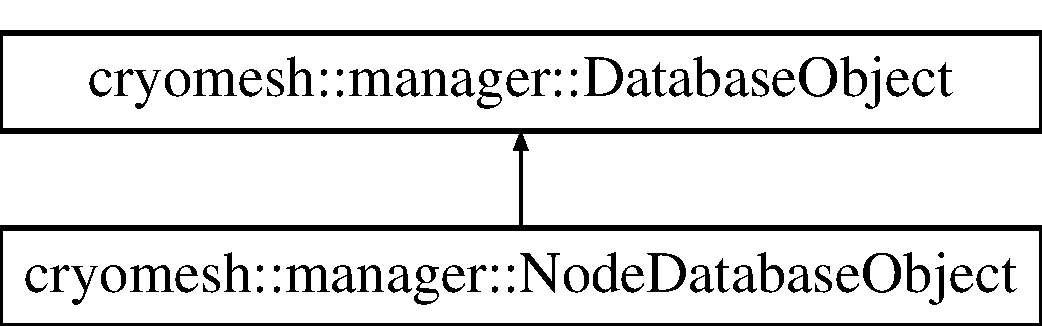
\includegraphics[height=2.000000cm]{classcryomesh_1_1manager_1_1NodeDatabaseObject}
\end{center}
\end{figure}
\subsection*{\-Public \-Member \-Functions}
\begin{DoxyCompactItemize}
\item 
\hyperlink{classcryomesh_1_1manager_1_1NodeDatabaseObject_a69cbe2fb91ca27e0b167165c52d11231}{\-Node\-Database\-Object} (std\-::string uuid\-\_\-str, spacial\-::\-Point pt, \hyperlink{classcryomesh_1_1common_1_1Cycle}{common\-::\-Cycle} cyc, double act)
\begin{DoxyCompactList}\small\item\em \-Create object from node variables. \end{DoxyCompactList}\item 
\hyperlink{classcryomesh_1_1manager_1_1NodeDatabaseObject_a96ec12a3290ce621734fb5695a4ca5c1}{\-Node\-Database\-Object} (const std\-::string \&node\-\_\-table\-\_\-entry)
\begin{DoxyCompactList}\small\item\em \-Create object from the string of entries in the database node table. \end{DoxyCompactList}\item 
virtual \hyperlink{classcryomesh_1_1manager_1_1NodeDatabaseObject_a1a9157f719dfef63441e0bc1d3c9a86e}{$\sim$\-Node\-Database\-Object} ()
\begin{DoxyCompactList}\small\item\em \-Default destructor. \end{DoxyCompactList}\item 
virtual std\-::string \hyperlink{classcryomesh_1_1manager_1_1NodeDatabaseObject_ac5512082d08fa59cbaa496b711f4c8c2}{get\-Insert} (const std\-::string \&table) const 
\begin{DoxyCompactList}\small\item\em \-Get the string that can be used to insert the sql data. \end{DoxyCompactList}\item 
std\-::string \hyperlink{classcryomesh_1_1manager_1_1NodeDatabaseObject_a57b4da149aa2ac3ea49b6cb10b06afda}{get\-U\-U\-I\-D} () const 
\begin{DoxyCompactList}\small\item\em \-Get uuid variable. \end{DoxyCompactList}\item 
const spacial\-::\-Point \& \hyperlink{classcryomesh_1_1manager_1_1NodeDatabaseObject_a8271688dc70be0b476f4890633d99fb0}{get\-Point} () const 
\begin{DoxyCompactList}\small\item\em \-Get point variable. \end{DoxyCompactList}\item 
const \hyperlink{classcryomesh_1_1common_1_1Cycle}{common\-::\-Cycle} \& \hyperlink{classcryomesh_1_1manager_1_1NodeDatabaseObject_a55fe6f939ab39a2db10fcf27681ef39e}{get\-Cycle} () const 
\begin{DoxyCompactList}\small\item\em \-Get cycle variable. \end{DoxyCompactList}\item 
double \hyperlink{classcryomesh_1_1manager_1_1NodeDatabaseObject_ac5bc1d274dbaa92abaec9ed59e05d805}{get\-Activity} () const 
\begin{DoxyCompactList}\small\item\em \-Get activity variable. \end{DoxyCompactList}\item 
std\-::string \hyperlink{classcryomesh_1_1manager_1_1DatabaseObject_a66ded4e1a1bccd65c94922648c7135c5}{get\-Key} (const std\-::string \&key) const 
\begin{DoxyCompactList}\small\item\em \-Return the string object associated with a key. \end{DoxyCompactList}\end{DoxyCompactItemize}
\subsection*{\-Static \-Public \-Member \-Functions}
\begin{DoxyCompactItemize}
\item 
static std\-::string \hyperlink{classcryomesh_1_1manager_1_1DatabaseObject_aa4ef26ce91fea092f146e67add491e0f}{find\-Value} (const std\-::string \&entry, const std\-::map$<$ std\-::string, std\-::string $>$ \&map)
\begin{DoxyCompactList}\small\item\em \-Find entries value in map or return null. \end{DoxyCompactList}\item 
static std\-::map$<$ std\-::string, \*
std\-::string $>$ \hyperlink{classcryomesh_1_1manager_1_1DatabaseObject_a04ce7c34b51e3290c972121cf2f16565}{get\-Column\-Map\-From\-Entry} (const std\-::string \&entry)
\begin{DoxyCompactList}\small\item\em \-Parse a string database entry, extract columns and values and return a map. \end{DoxyCompactList}\item 
{\footnotesize template$<$class T $>$ }\\static std\-::string \hyperlink{classcryomesh_1_1manager_1_1DatabaseObject_a1b37d9d07009ae1c71f644761d36b468}{to\-String} (\-T obj)
\begin{DoxyCompactList}\small\item\em \-Convert an templated object that can be piped to a stream to a string. \end{DoxyCompactList}\end{DoxyCompactItemize}
\subsection*{\-Static \-Public \-Attributes}
\begin{DoxyCompactItemize}
\item 
static const std\-::string \hyperlink{classcryomesh_1_1manager_1_1NodeDatabaseObject_ac46a43bc3578edde244684a90c0347c6}{\-I\-D\-\_\-\-T\-A\-G} = \char`\"{}id\char`\"{}
\item 
static const std\-::string \hyperlink{classcryomesh_1_1manager_1_1NodeDatabaseObject_a13b5bc3d98b96aaf13946d894ee198da}{\-X\-\_\-\-T\-A\-G} = \char`\"{}x\char`\"{}
\item 
static const std\-::string \hyperlink{classcryomesh_1_1manager_1_1NodeDatabaseObject_a53f9eddc7a4946d85d3c2a873b501fb4}{\-Y\-\_\-\-T\-A\-G} = \char`\"{}y\char`\"{}
\item 
static const std\-::string \hyperlink{classcryomesh_1_1manager_1_1NodeDatabaseObject_a6ad97b44dd2f10fd83db1c62283f5bdd}{\-Z\-\_\-\-T\-A\-G} = \char`\"{}z\char`\"{}
\item 
static const std\-::string \hyperlink{classcryomesh_1_1manager_1_1NodeDatabaseObject_a5b88df8ce26dc6ee6b7f2fd369ee88d7}{\-A\-C\-T\-I\-V\-I\-T\-Y\-\_\-\-T\-A\-G} = \char`\"{}activity\char`\"{}
\item 
static const std\-::string \hyperlink{classcryomesh_1_1manager_1_1NodeDatabaseObject_a27dbca85d042b1bf292de812e3da608c}{\-C\-Y\-C\-L\-E\-\_\-\-T\-A\-G} = \char`\"{}cycle\char`\"{}
\end{DoxyCompactItemize}
\subsection*{\-Protected \-Attributes}
\begin{DoxyCompactItemize}
\item 
std\-::map$<$ std\-::string, \*
std\-::string $>$ \hyperlink{classcryomesh_1_1manager_1_1DatabaseObject_a9c648bf09b9fd8b4d599b0d4f4abf531}{columns}
\end{DoxyCompactItemize}
\subsection*{\-Private \-Attributes}
\begin{DoxyCompactItemize}
\item 
std\-::string \hyperlink{classcryomesh_1_1manager_1_1NodeDatabaseObject_a26f7172c0939529683f5ffcba9bf18f7}{uuid}
\item 
spacial\-::\-Point \hyperlink{classcryomesh_1_1manager_1_1NodeDatabaseObject_ae3f66b98b554fb2ef839e18b4d2a6e28}{point}
\item 
\hyperlink{classcryomesh_1_1common_1_1Cycle}{common\-::\-Cycle} \hyperlink{classcryomesh_1_1manager_1_1NodeDatabaseObject_a64c6887b55673bfb0dcd49919c2f21f8}{cycle}
\item 
double \hyperlink{classcryomesh_1_1manager_1_1NodeDatabaseObject_a058afbf0cba44ece21b40f30a6ff31a1}{activity}
\end{DoxyCompactItemize}


\subsection{\-Detailed \-Description}


\-Definition at line 20 of file \-Node\-Database\-Object.\-h.



\subsection{\-Constructor \& \-Destructor \-Documentation}
\hypertarget{classcryomesh_1_1manager_1_1NodeDatabaseObject_a69cbe2fb91ca27e0b167165c52d11231}{\index{cryomesh\-::manager\-::\-Node\-Database\-Object@{cryomesh\-::manager\-::\-Node\-Database\-Object}!\-Node\-Database\-Object@{\-Node\-Database\-Object}}
\index{\-Node\-Database\-Object@{\-Node\-Database\-Object}!cryomesh::manager::NodeDatabaseObject@{cryomesh\-::manager\-::\-Node\-Database\-Object}}
\subsubsection[{\-Node\-Database\-Object}]{\setlength{\rightskip}{0pt plus 5cm}{\bf cryomesh\-::manager\-::\-Node\-Database\-Object\-::\-Node\-Database\-Object} (
\begin{DoxyParamCaption}
\item[{std\-::string}]{uuid\-\_\-str, }
\item[{spacial\-::\-Point}]{pt, }
\item[{{\bf common\-::\-Cycle}}]{cyc, }
\item[{double}]{act}
\end{DoxyParamCaption}
)}}\label{classcryomesh_1_1manager_1_1NodeDatabaseObject_a69cbe2fb91ca27e0b167165c52d11231}


\-Create object from node variables. 


\begin{DoxyParams}{\-Parameters}
{\em std\-::string} & \-The uuid string of the node \\
\hline
{\em spacial\-::\-Point} & \-Location of the node \\
\hline
{\em \-Cycle} & \-The cycle of the entry \\
\hline
{\em double} & \-The activity of the node on the cycle \\
\hline
\end{DoxyParams}


\-Definition at line 13 of file \-Node\-Database\-Object.\-cpp.



\-References activity, \-A\-C\-T\-I\-V\-I\-T\-Y\-\_\-\-T\-A\-G, cryomesh\-::manager\-::\-Database\-Object\-::columns, cycle, \-C\-Y\-C\-L\-E\-\_\-\-T\-A\-G, \-I\-D\-\_\-\-T\-A\-G, point, cryomesh\-::common\-::\-Cycle\-::to\-U\-L\-Int(), \-X\-\_\-\-T\-A\-G, \-Y\-\_\-\-T\-A\-G, and \-Z\-\_\-\-T\-A\-G.

\hypertarget{classcryomesh_1_1manager_1_1NodeDatabaseObject_a96ec12a3290ce621734fb5695a4ca5c1}{\index{cryomesh\-::manager\-::\-Node\-Database\-Object@{cryomesh\-::manager\-::\-Node\-Database\-Object}!\-Node\-Database\-Object@{\-Node\-Database\-Object}}
\index{\-Node\-Database\-Object@{\-Node\-Database\-Object}!cryomesh::manager::NodeDatabaseObject@{cryomesh\-::manager\-::\-Node\-Database\-Object}}
\subsubsection[{\-Node\-Database\-Object}]{\setlength{\rightskip}{0pt plus 5cm}{\bf cryomesh\-::manager\-::\-Node\-Database\-Object\-::\-Node\-Database\-Object} (
\begin{DoxyParamCaption}
\item[{const std\-::string \&}]{node\-\_\-table\-\_\-entry}
\end{DoxyParamCaption}
)}}\label{classcryomesh_1_1manager_1_1NodeDatabaseObject_a96ec12a3290ce621734fb5695a4ca5c1}


\-Create object from the string of entries in the database node table. 


\begin{DoxyParams}{\-Parameters}
{\em std\-::string} & \-The string of data taken from a node entry in the database node table \\
\hline
\end{DoxyParams}


\-Definition at line 23 of file \-Node\-Database\-Object.\-cpp.



\-References activity, cycle, cryomesh\-::manager\-::\-Database\-Object\-::find\-Value(), cryomesh\-::manager\-::\-Database\-Object\-::get\-Column\-Map\-From\-Entry(), point, and uuid.

\hypertarget{classcryomesh_1_1manager_1_1NodeDatabaseObject_a1a9157f719dfef63441e0bc1d3c9a86e}{\index{cryomesh\-::manager\-::\-Node\-Database\-Object@{cryomesh\-::manager\-::\-Node\-Database\-Object}!$\sim$\-Node\-Database\-Object@{$\sim$\-Node\-Database\-Object}}
\index{$\sim$\-Node\-Database\-Object@{$\sim$\-Node\-Database\-Object}!cryomesh::manager::NodeDatabaseObject@{cryomesh\-::manager\-::\-Node\-Database\-Object}}
\subsubsection[{$\sim$\-Node\-Database\-Object}]{\setlength{\rightskip}{0pt plus 5cm}{\bf cryomesh\-::manager\-::\-Node\-Database\-Object\-::$\sim$\-Node\-Database\-Object} (
\begin{DoxyParamCaption}
{}
\end{DoxyParamCaption}
)\hspace{0.3cm}{\ttfamily  \mbox{[}virtual\mbox{]}}}}\label{classcryomesh_1_1manager_1_1NodeDatabaseObject_a1a9157f719dfef63441e0bc1d3c9a86e}


\-Default destructor. 



\-Definition at line 60 of file \-Node\-Database\-Object.\-cpp.



\subsection{\-Member \-Function \-Documentation}
\hypertarget{classcryomesh_1_1manager_1_1DatabaseObject_aa4ef26ce91fea092f146e67add491e0f}{\index{cryomesh\-::manager\-::\-Node\-Database\-Object@{cryomesh\-::manager\-::\-Node\-Database\-Object}!find\-Value@{find\-Value}}
\index{find\-Value@{find\-Value}!cryomesh::manager::NodeDatabaseObject@{cryomesh\-::manager\-::\-Node\-Database\-Object}}
\subsubsection[{find\-Value}]{\setlength{\rightskip}{0pt plus 5cm}static std\-::string {\bf cryomesh\-::manager\-::\-Database\-Object\-::find\-Value} (
\begin{DoxyParamCaption}
\item[{const std\-::string \&}]{entry, }
\item[{const std\-::map$<$ std\-::string, std\-::string $>$ \&}]{map}
\end{DoxyParamCaption}
)\hspace{0.3cm}{\ttfamily  \mbox{[}inline, static, inherited\mbox{]}}}}\label{classcryomesh_1_1manager_1_1DatabaseObject_aa4ef26ce91fea092f146e67add491e0f}


\-Find entries value in map or return null. 


\begin{DoxyParams}{\-Parameters}
{\em std\-::string} & \-Entry to find \\
\hline
{\em std\-::map$<$std\-::string,std\-::string} & map to search\\
\hline
\end{DoxyParams}
\begin{DoxyReturn}{\-Returns}
\-Value of entry 
\end{DoxyReturn}


\-Definition at line 59 of file \-Database\-Object.\-h.



\-Referenced by cryomesh\-::manager\-::\-Connection\-Database\-Object\-::\-Connection\-Database\-Object(), \-Node\-Database\-Object(), and cryomesh\-::manager\-::\-Pattern\-Database\-Object\-::\-Pattern\-Database\-Object().

\hypertarget{classcryomesh_1_1manager_1_1NodeDatabaseObject_ac5bc1d274dbaa92abaec9ed59e05d805}{\index{cryomesh\-::manager\-::\-Node\-Database\-Object@{cryomesh\-::manager\-::\-Node\-Database\-Object}!get\-Activity@{get\-Activity}}
\index{get\-Activity@{get\-Activity}!cryomesh::manager::NodeDatabaseObject@{cryomesh\-::manager\-::\-Node\-Database\-Object}}
\subsubsection[{get\-Activity}]{\setlength{\rightskip}{0pt plus 5cm}double {\bf cryomesh\-::manager\-::\-Node\-Database\-Object\-::get\-Activity} (
\begin{DoxyParamCaption}
{}
\end{DoxyParamCaption}
) const}}\label{classcryomesh_1_1manager_1_1NodeDatabaseObject_ac5bc1d274dbaa92abaec9ed59e05d805}


\-Get activity variable. 

\begin{DoxyReturn}{\-Returns}
double \-The activity variable 
\end{DoxyReturn}


\-Definition at line 83 of file \-Node\-Database\-Object.\-cpp.



\-References activity.

\hypertarget{classcryomesh_1_1manager_1_1DatabaseObject_a04ce7c34b51e3290c972121cf2f16565}{\index{cryomesh\-::manager\-::\-Node\-Database\-Object@{cryomesh\-::manager\-::\-Node\-Database\-Object}!get\-Column\-Map\-From\-Entry@{get\-Column\-Map\-From\-Entry}}
\index{get\-Column\-Map\-From\-Entry@{get\-Column\-Map\-From\-Entry}!cryomesh::manager::NodeDatabaseObject@{cryomesh\-::manager\-::\-Node\-Database\-Object}}
\subsubsection[{get\-Column\-Map\-From\-Entry}]{\setlength{\rightskip}{0pt plus 5cm}static std\-::map$<$std\-::string, std\-::string$>$ {\bf cryomesh\-::manager\-::\-Database\-Object\-::get\-Column\-Map\-From\-Entry} (
\begin{DoxyParamCaption}
\item[{const std\-::string \&}]{entry}
\end{DoxyParamCaption}
)\hspace{0.3cm}{\ttfamily  \mbox{[}inline, static, inherited\mbox{]}}}}\label{classcryomesh_1_1manager_1_1DatabaseObject_a04ce7c34b51e3290c972121cf2f16565}


\-Parse a string database entry, extract columns and values and return a map. 



\-Definition at line 72 of file \-Database\-Object.\-h.



\-Referenced by cryomesh\-::manager\-::\-Connection\-Database\-Object\-::\-Connection\-Database\-Object(), \-Node\-Database\-Object(), and cryomesh\-::manager\-::\-Pattern\-Database\-Object\-::\-Pattern\-Database\-Object().

\hypertarget{classcryomesh_1_1manager_1_1NodeDatabaseObject_a55fe6f939ab39a2db10fcf27681ef39e}{\index{cryomesh\-::manager\-::\-Node\-Database\-Object@{cryomesh\-::manager\-::\-Node\-Database\-Object}!get\-Cycle@{get\-Cycle}}
\index{get\-Cycle@{get\-Cycle}!cryomesh::manager::NodeDatabaseObject@{cryomesh\-::manager\-::\-Node\-Database\-Object}}
\subsubsection[{get\-Cycle}]{\setlength{\rightskip}{0pt plus 5cm}const {\bf common\-::\-Cycle} \& {\bf cryomesh\-::manager\-::\-Node\-Database\-Object\-::get\-Cycle} (
\begin{DoxyParamCaption}
{}
\end{DoxyParamCaption}
) const}}\label{classcryomesh_1_1manager_1_1NodeDatabaseObject_a55fe6f939ab39a2db10fcf27681ef39e}


\-Get cycle variable. 

\begin{DoxyReturn}{\-Returns}
\hyperlink{classcryomesh_1_1common_1_1Cycle}{common\-::\-Cycle} \-The cycle variable 
\end{DoxyReturn}


\-Definition at line 80 of file \-Node\-Database\-Object.\-cpp.



\-References cycle.

\hypertarget{classcryomesh_1_1manager_1_1NodeDatabaseObject_ac5512082d08fa59cbaa496b711f4c8c2}{\index{cryomesh\-::manager\-::\-Node\-Database\-Object@{cryomesh\-::manager\-::\-Node\-Database\-Object}!get\-Insert@{get\-Insert}}
\index{get\-Insert@{get\-Insert}!cryomesh::manager::NodeDatabaseObject@{cryomesh\-::manager\-::\-Node\-Database\-Object}}
\subsubsection[{get\-Insert}]{\setlength{\rightskip}{0pt plus 5cm}std\-::string {\bf cryomesh\-::manager\-::\-Node\-Database\-Object\-::get\-Insert} (
\begin{DoxyParamCaption}
\item[{const std\-::string \&}]{table}
\end{DoxyParamCaption}
) const\hspace{0.3cm}{\ttfamily  \mbox{[}virtual\mbox{]}}}}\label{classcryomesh_1_1manager_1_1NodeDatabaseObject_ac5512082d08fa59cbaa496b711f4c8c2}


\-Get the string that can be used to insert the sql data. 

\begin{DoxyReturn}{\-Returns}
the sql command string to insert into this table 
\end{DoxyReturn}


\-Implements \hyperlink{classcryomesh_1_1manager_1_1DatabaseObject_ad55c6e711341a652790b97f549b0dc63}{cryomesh\-::manager\-::\-Database\-Object}.



\-Definition at line 63 of file \-Node\-Database\-Object.\-cpp.



\-References \-A\-C\-T\-I\-V\-I\-T\-Y\-\_\-\-T\-A\-G, \-C\-Y\-C\-L\-E\-\_\-\-T\-A\-G, cryomesh\-::manager\-::\-Database\-Object\-::get\-Key(), \-I\-D\-\_\-\-T\-A\-G, \-X\-\_\-\-T\-A\-G, \-Y\-\_\-\-T\-A\-G, and \-Z\-\_\-\-T\-A\-G.

\hypertarget{classcryomesh_1_1manager_1_1DatabaseObject_a66ded4e1a1bccd65c94922648c7135c5}{\index{cryomesh\-::manager\-::\-Node\-Database\-Object@{cryomesh\-::manager\-::\-Node\-Database\-Object}!get\-Key@{get\-Key}}
\index{get\-Key@{get\-Key}!cryomesh::manager::NodeDatabaseObject@{cryomesh\-::manager\-::\-Node\-Database\-Object}}
\subsubsection[{get\-Key}]{\setlength{\rightskip}{0pt plus 5cm}std\-::string {\bf cryomesh\-::manager\-::\-Database\-Object\-::get\-Key} (
\begin{DoxyParamCaption}
\item[{const std\-::string \&}]{key}
\end{DoxyParamCaption}
) const\hspace{0.3cm}{\ttfamily  \mbox{[}inline, inherited\mbox{]}}}}\label{classcryomesh_1_1manager_1_1DatabaseObject_a66ded4e1a1bccd65c94922648c7135c5}


\-Return the string object associated with a key. 

\-::string \-The key to search for

\begin{DoxyReturn}{\-Returns}
std\-::string \-The object associated with the search key, \char`\"{}\char`\"{} if not found 
\end{DoxyReturn}


\-Definition at line 37 of file \-Database\-Object.\-h.



\-References cryomesh\-::manager\-::\-Database\-Object\-::columns.



\-Referenced by cryomesh\-::manager\-::\-Pattern\-Database\-Object\-::get\-Insert(), get\-Insert(), and cryomesh\-::manager\-::\-Connection\-Database\-Object\-::get\-Insert().

\hypertarget{classcryomesh_1_1manager_1_1NodeDatabaseObject_a8271688dc70be0b476f4890633d99fb0}{\index{cryomesh\-::manager\-::\-Node\-Database\-Object@{cryomesh\-::manager\-::\-Node\-Database\-Object}!get\-Point@{get\-Point}}
\index{get\-Point@{get\-Point}!cryomesh::manager::NodeDatabaseObject@{cryomesh\-::manager\-::\-Node\-Database\-Object}}
\subsubsection[{get\-Point}]{\setlength{\rightskip}{0pt plus 5cm}const spacial\-::\-Point \& {\bf cryomesh\-::manager\-::\-Node\-Database\-Object\-::get\-Point} (
\begin{DoxyParamCaption}
{}
\end{DoxyParamCaption}
) const}}\label{classcryomesh_1_1manager_1_1NodeDatabaseObject_a8271688dc70be0b476f4890633d99fb0}


\-Get point variable. 

\begin{DoxyReturn}{\-Returns}
spacial\-::\-Point \-The point variable 
\end{DoxyReturn}


\-Definition at line 77 of file \-Node\-Database\-Object.\-cpp.



\-References point.

\hypertarget{classcryomesh_1_1manager_1_1NodeDatabaseObject_a57b4da149aa2ac3ea49b6cb10b06afda}{\index{cryomesh\-::manager\-::\-Node\-Database\-Object@{cryomesh\-::manager\-::\-Node\-Database\-Object}!get\-U\-U\-I\-D@{get\-U\-U\-I\-D}}
\index{get\-U\-U\-I\-D@{get\-U\-U\-I\-D}!cryomesh::manager::NodeDatabaseObject@{cryomesh\-::manager\-::\-Node\-Database\-Object}}
\subsubsection[{get\-U\-U\-I\-D}]{\setlength{\rightskip}{0pt plus 5cm}std\-::string {\bf cryomesh\-::manager\-::\-Node\-Database\-Object\-::get\-U\-U\-I\-D} (
\begin{DoxyParamCaption}
{}
\end{DoxyParamCaption}
) const}}\label{classcryomesh_1_1manager_1_1NodeDatabaseObject_a57b4da149aa2ac3ea49b6cb10b06afda}


\-Get uuid variable. 

\begin{DoxyReturn}{\-Returns}
std\-::string \-The uuid variable 
\end{DoxyReturn}


\-Definition at line 74 of file \-Node\-Database\-Object.\-cpp.



\-References uuid.

\hypertarget{classcryomesh_1_1manager_1_1DatabaseObject_a1b37d9d07009ae1c71f644761d36b468}{\index{cryomesh\-::manager\-::\-Node\-Database\-Object@{cryomesh\-::manager\-::\-Node\-Database\-Object}!to\-String@{to\-String}}
\index{to\-String@{to\-String}!cryomesh::manager::NodeDatabaseObject@{cryomesh\-::manager\-::\-Node\-Database\-Object}}
\subsubsection[{to\-String}]{\setlength{\rightskip}{0pt plus 5cm}template$<$class T $>$ static std\-::string {\bf cryomesh\-::manager\-::\-Database\-Object\-::to\-String} (
\begin{DoxyParamCaption}
\item[{\-T}]{obj}
\end{DoxyParamCaption}
)\hspace{0.3cm}{\ttfamily  \mbox{[}inline, static, inherited\mbox{]}}}}\label{classcryomesh_1_1manager_1_1DatabaseObject_a1b37d9d07009ae1c71f644761d36b468}


\-Convert an templated object that can be piped to a stream to a string. 


\begin{DoxyParams}{\-Parameters}
{\em \-T} & \-The object to get a string for \\
\hline
\end{DoxyParams}


\-Definition at line 108 of file \-Database\-Object.\-h.



\subsection{\-Member \-Data \-Documentation}
\hypertarget{classcryomesh_1_1manager_1_1NodeDatabaseObject_a058afbf0cba44ece21b40f30a6ff31a1}{\index{cryomesh\-::manager\-::\-Node\-Database\-Object@{cryomesh\-::manager\-::\-Node\-Database\-Object}!activity@{activity}}
\index{activity@{activity}!cryomesh::manager::NodeDatabaseObject@{cryomesh\-::manager\-::\-Node\-Database\-Object}}
\subsubsection[{activity}]{\setlength{\rightskip}{0pt plus 5cm}double {\bf cryomesh\-::manager\-::\-Node\-Database\-Object\-::activity}\hspace{0.3cm}{\ttfamily  \mbox{[}private\mbox{]}}}}\label{classcryomesh_1_1manager_1_1NodeDatabaseObject_a058afbf0cba44ece21b40f30a6ff31a1}


\-Definition at line 158 of file \-Node\-Database\-Object.\-h.



\-Referenced by get\-Activity(), and \-Node\-Database\-Object().

\hypertarget{classcryomesh_1_1manager_1_1NodeDatabaseObject_a5b88df8ce26dc6ee6b7f2fd369ee88d7}{\index{cryomesh\-::manager\-::\-Node\-Database\-Object@{cryomesh\-::manager\-::\-Node\-Database\-Object}!\-A\-C\-T\-I\-V\-I\-T\-Y\-\_\-\-T\-A\-G@{\-A\-C\-T\-I\-V\-I\-T\-Y\-\_\-\-T\-A\-G}}
\index{\-A\-C\-T\-I\-V\-I\-T\-Y\-\_\-\-T\-A\-G@{\-A\-C\-T\-I\-V\-I\-T\-Y\-\_\-\-T\-A\-G}!cryomesh::manager::NodeDatabaseObject@{cryomesh\-::manager\-::\-Node\-Database\-Object}}
\subsubsection[{\-A\-C\-T\-I\-V\-I\-T\-Y\-\_\-\-T\-A\-G}]{\setlength{\rightskip}{0pt plus 5cm}const std\-::string {\bf cryomesh\-::manager\-::\-Node\-Database\-Object\-::\-A\-C\-T\-I\-V\-I\-T\-Y\-\_\-\-T\-A\-G} = \char`\"{}activity\char`\"{}\hspace{0.3cm}{\ttfamily  \mbox{[}static\mbox{]}}}}\label{classcryomesh_1_1manager_1_1NodeDatabaseObject_a5b88df8ce26dc6ee6b7f2fd369ee88d7}


\-Definition at line 122 of file \-Node\-Database\-Object.\-h.



\-Referenced by get\-Insert(), and \-Node\-Database\-Object().

\hypertarget{classcryomesh_1_1manager_1_1DatabaseObject_a9c648bf09b9fd8b4d599b0d4f4abf531}{\index{cryomesh\-::manager\-::\-Node\-Database\-Object@{cryomesh\-::manager\-::\-Node\-Database\-Object}!columns@{columns}}
\index{columns@{columns}!cryomesh::manager::NodeDatabaseObject@{cryomesh\-::manager\-::\-Node\-Database\-Object}}
\subsubsection[{columns}]{\setlength{\rightskip}{0pt plus 5cm}std\-::map$<$std\-::string, std\-::string$>$ {\bf cryomesh\-::manager\-::\-Database\-Object\-::columns}\hspace{0.3cm}{\ttfamily  \mbox{[}protected, inherited\mbox{]}}}}\label{classcryomesh_1_1manager_1_1DatabaseObject_a9c648bf09b9fd8b4d599b0d4f4abf531}


\-Definition at line 119 of file \-Database\-Object.\-h.



\-Referenced by cryomesh\-::manager\-::\-Connection\-Database\-Object\-::\-Connection\-Database\-Object(), cryomesh\-::manager\-::\-Database\-Object\-::get\-Key(), \-Node\-Database\-Object(), and cryomesh\-::manager\-::\-Pattern\-Database\-Object\-::\-Pattern\-Database\-Object().

\hypertarget{classcryomesh_1_1manager_1_1NodeDatabaseObject_a64c6887b55673bfb0dcd49919c2f21f8}{\index{cryomesh\-::manager\-::\-Node\-Database\-Object@{cryomesh\-::manager\-::\-Node\-Database\-Object}!cycle@{cycle}}
\index{cycle@{cycle}!cryomesh::manager::NodeDatabaseObject@{cryomesh\-::manager\-::\-Node\-Database\-Object}}
\subsubsection[{cycle}]{\setlength{\rightskip}{0pt plus 5cm}{\bf common\-::\-Cycle} {\bf cryomesh\-::manager\-::\-Node\-Database\-Object\-::cycle}\hspace{0.3cm}{\ttfamily  \mbox{[}private\mbox{]}}}}\label{classcryomesh_1_1manager_1_1NodeDatabaseObject_a64c6887b55673bfb0dcd49919c2f21f8}


\-Definition at line 151 of file \-Node\-Database\-Object.\-h.



\-Referenced by get\-Cycle(), and \-Node\-Database\-Object().

\hypertarget{classcryomesh_1_1manager_1_1NodeDatabaseObject_a27dbca85d042b1bf292de812e3da608c}{\index{cryomesh\-::manager\-::\-Node\-Database\-Object@{cryomesh\-::manager\-::\-Node\-Database\-Object}!\-C\-Y\-C\-L\-E\-\_\-\-T\-A\-G@{\-C\-Y\-C\-L\-E\-\_\-\-T\-A\-G}}
\index{\-C\-Y\-C\-L\-E\-\_\-\-T\-A\-G@{\-C\-Y\-C\-L\-E\-\_\-\-T\-A\-G}!cryomesh::manager::NodeDatabaseObject@{cryomesh\-::manager\-::\-Node\-Database\-Object}}
\subsubsection[{\-C\-Y\-C\-L\-E\-\_\-\-T\-A\-G}]{\setlength{\rightskip}{0pt plus 5cm}const std\-::string {\bf cryomesh\-::manager\-::\-Node\-Database\-Object\-::\-C\-Y\-C\-L\-E\-\_\-\-T\-A\-G} = \char`\"{}cycle\char`\"{}\hspace{0.3cm}{\ttfamily  \mbox{[}static\mbox{]}}}}\label{classcryomesh_1_1manager_1_1NodeDatabaseObject_a27dbca85d042b1bf292de812e3da608c}


\-Definition at line 129 of file \-Node\-Database\-Object.\-h.



\-Referenced by get\-Insert(), and \-Node\-Database\-Object().

\hypertarget{classcryomesh_1_1manager_1_1NodeDatabaseObject_ac46a43bc3578edde244684a90c0347c6}{\index{cryomesh\-::manager\-::\-Node\-Database\-Object@{cryomesh\-::manager\-::\-Node\-Database\-Object}!\-I\-D\-\_\-\-T\-A\-G@{\-I\-D\-\_\-\-T\-A\-G}}
\index{\-I\-D\-\_\-\-T\-A\-G@{\-I\-D\-\_\-\-T\-A\-G}!cryomesh::manager::NodeDatabaseObject@{cryomesh\-::manager\-::\-Node\-Database\-Object}}
\subsubsection[{\-I\-D\-\_\-\-T\-A\-G}]{\setlength{\rightskip}{0pt plus 5cm}const std\-::string {\bf cryomesh\-::manager\-::\-Node\-Database\-Object\-::\-I\-D\-\_\-\-T\-A\-G} = \char`\"{}id\char`\"{}\hspace{0.3cm}{\ttfamily  \mbox{[}static\mbox{]}}}}\label{classcryomesh_1_1manager_1_1NodeDatabaseObject_ac46a43bc3578edde244684a90c0347c6}


\-Definition at line 94 of file \-Node\-Database\-Object.\-h.



\-Referenced by get\-Insert(), and \-Node\-Database\-Object().

\hypertarget{classcryomesh_1_1manager_1_1NodeDatabaseObject_ae3f66b98b554fb2ef839e18b4d2a6e28}{\index{cryomesh\-::manager\-::\-Node\-Database\-Object@{cryomesh\-::manager\-::\-Node\-Database\-Object}!point@{point}}
\index{point@{point}!cryomesh::manager::NodeDatabaseObject@{cryomesh\-::manager\-::\-Node\-Database\-Object}}
\subsubsection[{point}]{\setlength{\rightskip}{0pt plus 5cm}spacial\-::\-Point {\bf cryomesh\-::manager\-::\-Node\-Database\-Object\-::point}\hspace{0.3cm}{\ttfamily  \mbox{[}private\mbox{]}}}}\label{classcryomesh_1_1manager_1_1NodeDatabaseObject_ae3f66b98b554fb2ef839e18b4d2a6e28}


\-Definition at line 144 of file \-Node\-Database\-Object.\-h.



\-Referenced by get\-Point(), and \-Node\-Database\-Object().

\hypertarget{classcryomesh_1_1manager_1_1NodeDatabaseObject_a26f7172c0939529683f5ffcba9bf18f7}{\index{cryomesh\-::manager\-::\-Node\-Database\-Object@{cryomesh\-::manager\-::\-Node\-Database\-Object}!uuid@{uuid}}
\index{uuid@{uuid}!cryomesh::manager::NodeDatabaseObject@{cryomesh\-::manager\-::\-Node\-Database\-Object}}
\subsubsection[{uuid}]{\setlength{\rightskip}{0pt plus 5cm}std\-::string {\bf cryomesh\-::manager\-::\-Node\-Database\-Object\-::uuid}\hspace{0.3cm}{\ttfamily  \mbox{[}private\mbox{]}}}}\label{classcryomesh_1_1manager_1_1NodeDatabaseObject_a26f7172c0939529683f5ffcba9bf18f7}


\-Definition at line 137 of file \-Node\-Database\-Object.\-h.



\-Referenced by get\-U\-U\-I\-D(), and \-Node\-Database\-Object().

\hypertarget{classcryomesh_1_1manager_1_1NodeDatabaseObject_a13b5bc3d98b96aaf13946d894ee198da}{\index{cryomesh\-::manager\-::\-Node\-Database\-Object@{cryomesh\-::manager\-::\-Node\-Database\-Object}!\-X\-\_\-\-T\-A\-G@{\-X\-\_\-\-T\-A\-G}}
\index{\-X\-\_\-\-T\-A\-G@{\-X\-\_\-\-T\-A\-G}!cryomesh::manager::NodeDatabaseObject@{cryomesh\-::manager\-::\-Node\-Database\-Object}}
\subsubsection[{\-X\-\_\-\-T\-A\-G}]{\setlength{\rightskip}{0pt plus 5cm}const std\-::string {\bf cryomesh\-::manager\-::\-Node\-Database\-Object\-::\-X\-\_\-\-T\-A\-G} = \char`\"{}x\char`\"{}\hspace{0.3cm}{\ttfamily  \mbox{[}static\mbox{]}}}}\label{classcryomesh_1_1manager_1_1NodeDatabaseObject_a13b5bc3d98b96aaf13946d894ee198da}


\-Definition at line 101 of file \-Node\-Database\-Object.\-h.



\-Referenced by get\-Insert(), and \-Node\-Database\-Object().

\hypertarget{classcryomesh_1_1manager_1_1NodeDatabaseObject_a53f9eddc7a4946d85d3c2a873b501fb4}{\index{cryomesh\-::manager\-::\-Node\-Database\-Object@{cryomesh\-::manager\-::\-Node\-Database\-Object}!\-Y\-\_\-\-T\-A\-G@{\-Y\-\_\-\-T\-A\-G}}
\index{\-Y\-\_\-\-T\-A\-G@{\-Y\-\_\-\-T\-A\-G}!cryomesh::manager::NodeDatabaseObject@{cryomesh\-::manager\-::\-Node\-Database\-Object}}
\subsubsection[{\-Y\-\_\-\-T\-A\-G}]{\setlength{\rightskip}{0pt plus 5cm}const std\-::string {\bf cryomesh\-::manager\-::\-Node\-Database\-Object\-::\-Y\-\_\-\-T\-A\-G} = \char`\"{}y\char`\"{}\hspace{0.3cm}{\ttfamily  \mbox{[}static\mbox{]}}}}\label{classcryomesh_1_1manager_1_1NodeDatabaseObject_a53f9eddc7a4946d85d3c2a873b501fb4}


\-Definition at line 108 of file \-Node\-Database\-Object.\-h.



\-Referenced by get\-Insert(), and \-Node\-Database\-Object().

\hypertarget{classcryomesh_1_1manager_1_1NodeDatabaseObject_a6ad97b44dd2f10fd83db1c62283f5bdd}{\index{cryomesh\-::manager\-::\-Node\-Database\-Object@{cryomesh\-::manager\-::\-Node\-Database\-Object}!\-Z\-\_\-\-T\-A\-G@{\-Z\-\_\-\-T\-A\-G}}
\index{\-Z\-\_\-\-T\-A\-G@{\-Z\-\_\-\-T\-A\-G}!cryomesh::manager::NodeDatabaseObject@{cryomesh\-::manager\-::\-Node\-Database\-Object}}
\subsubsection[{\-Z\-\_\-\-T\-A\-G}]{\setlength{\rightskip}{0pt plus 5cm}const std\-::string {\bf cryomesh\-::manager\-::\-Node\-Database\-Object\-::\-Z\-\_\-\-T\-A\-G} = \char`\"{}z\char`\"{}\hspace{0.3cm}{\ttfamily  \mbox{[}static\mbox{]}}}}\label{classcryomesh_1_1manager_1_1NodeDatabaseObject_a6ad97b44dd2f10fd83db1c62283f5bdd}


\-Definition at line 115 of file \-Node\-Database\-Object.\-h.



\-Referenced by get\-Insert(), and \-Node\-Database\-Object().



\-The documentation for this class was generated from the following files\-:\begin{DoxyCompactItemize}
\item 
/home/niall/\-Projects/\-Eclipse/\-C\-P\-P/cryomesh/src/manager/\hyperlink{NodeDatabaseObject_8h}{\-Node\-Database\-Object.\-h}\item 
/home/niall/\-Projects/\-Eclipse/\-C\-P\-P/cryomesh/src/manager/\hyperlink{NodeDatabaseObject_8cpp}{\-Node\-Database\-Object.\-cpp}\end{DoxyCompactItemize}

\hypertarget{structcryomesh_1_1utilities_1_1SequencerGeneric_1_1NodeEntry}{\section{cryomesh\-:\-:utilities\-:\-:\-Sequencer\-Generic\-:\-:\-Node\-Entry \-Struct \-Reference}
\label{structcryomesh_1_1utilities_1_1SequencerGeneric_1_1NodeEntry}\index{cryomesh\-::utilities\-::\-Sequencer\-Generic\-::\-Node\-Entry@{cryomesh\-::utilities\-::\-Sequencer\-Generic\-::\-Node\-Entry}}
}


{\ttfamily \#include $<$\-Sequencer\-Generic.\-h$>$}

\subsection*{\-Public \-Member \-Functions}
\begin{DoxyCompactItemize}
\item 
\hyperlink{structcryomesh_1_1utilities_1_1SequencerGeneric_1_1NodeEntry_a09783531f959f6f240446bf9247affd7}{\-Node\-Entry} ()
\end{DoxyCompactItemize}
\subsection*{\-Public \-Attributes}
\begin{DoxyCompactItemize}
\item 
std\-::string \hyperlink{structcryomesh_1_1utilities_1_1SequencerGeneric_1_1NodeEntry_ac7bdacc33badb83a8599ac90a94b25aa}{name}
\item 
std\-::map$<$ std\-::string, \*
std\-::string $>$ \hyperlink{structcryomesh_1_1utilities_1_1SequencerGeneric_1_1NodeEntry_a902d9ca7a5864a758bae3e9eb9de711a}{info}
\item 
boost\-::shared\-\_\-ptr$<$ \hyperlink{structcryomesh_1_1utilities_1_1SequencerGeneric_1_1NodeEntry}{\-Node\-Entry} $>$ \hyperlink{structcryomesh_1_1utilities_1_1SequencerGeneric_1_1NodeEntry_ad243d1b3137d6601cb413a43761ac073}{parent\-Node}
\item 
std\-::list$<$ boost\-::shared\-\_\-ptr\*
$<$ \hyperlink{structcryomesh_1_1utilities_1_1SequencerGeneric_1_1NodeEntry}{\-Node\-Entry} $>$ $>$ \hyperlink{structcryomesh_1_1utilities_1_1SequencerGeneric_1_1NodeEntry_aa81743684d922c5af1dca8c15923d272}{child\-Nodes}
\end{DoxyCompactItemize}
\subsection*{\-Friends}
\begin{DoxyCompactItemize}
\item 
std\-::ostream \& \hyperlink{structcryomesh_1_1utilities_1_1SequencerGeneric_1_1NodeEntry_a0f3acff395102a2a1b89879932088968}{operator$<$$<$} (std\-::ostream \&os, const \hyperlink{structcryomesh_1_1utilities_1_1SequencerGeneric_1_1NodeEntry}{\-Node\-Entry} \&obj)
\end{DoxyCompactItemize}


\subsection{\-Detailed \-Description}


\-Definition at line 14 of file \-Sequencer\-Generic.\-h.



\subsection{\-Constructor \& \-Destructor \-Documentation}
\hypertarget{structcryomesh_1_1utilities_1_1SequencerGeneric_1_1NodeEntry_a09783531f959f6f240446bf9247affd7}{\index{cryomesh\-::utilities\-::\-Sequencer\-Generic\-::\-Node\-Entry@{cryomesh\-::utilities\-::\-Sequencer\-Generic\-::\-Node\-Entry}!\-Node\-Entry@{\-Node\-Entry}}
\index{\-Node\-Entry@{\-Node\-Entry}!cryomesh::utilities::SequencerGeneric::NodeEntry@{cryomesh\-::utilities\-::\-Sequencer\-Generic\-::\-Node\-Entry}}
\subsubsection[{\-Node\-Entry}]{\setlength{\rightskip}{0pt plus 5cm}{\bf cryomesh\-::utilities\-::\-Sequencer\-Generic\-::\-Node\-Entry\-::\-Node\-Entry} (
\begin{DoxyParamCaption}
{}
\end{DoxyParamCaption}
)\hspace{0.3cm}{\ttfamily  \mbox{[}inline\mbox{]}}}}\label{structcryomesh_1_1utilities_1_1SequencerGeneric_1_1NodeEntry_a09783531f959f6f240446bf9247affd7}


\-Definition at line 16 of file \-Sequencer\-Generic.\-h.



\subsection{\-Friends \-And \-Related \-Function \-Documentation}
\hypertarget{structcryomesh_1_1utilities_1_1SequencerGeneric_1_1NodeEntry_a0f3acff395102a2a1b89879932088968}{\index{cryomesh\-::utilities\-::\-Sequencer\-Generic\-::\-Node\-Entry@{cryomesh\-::utilities\-::\-Sequencer\-Generic\-::\-Node\-Entry}!operator$<$$<$@{operator$<$$<$}}
\index{operator$<$$<$@{operator$<$$<$}!cryomesh::utilities::SequencerGeneric::NodeEntry@{cryomesh\-::utilities\-::\-Sequencer\-Generic\-::\-Node\-Entry}}
\subsubsection[{operator$<$$<$}]{\setlength{\rightskip}{0pt plus 5cm}std\-::ostream\& operator$<$$<$ (
\begin{DoxyParamCaption}
\item[{std\-::ostream \&}]{os, }
\item[{const {\bf \-Node\-Entry} \&}]{obj}
\end{DoxyParamCaption}
)\hspace{0.3cm}{\ttfamily  \mbox{[}friend\mbox{]}}}}\label{structcryomesh_1_1utilities_1_1SequencerGeneric_1_1NodeEntry_a0f3acff395102a2a1b89879932088968}


\-Definition at line 23 of file \-Sequencer\-Generic.\-h.



\subsection{\-Member \-Data \-Documentation}
\hypertarget{structcryomesh_1_1utilities_1_1SequencerGeneric_1_1NodeEntry_aa81743684d922c5af1dca8c15923d272}{\index{cryomesh\-::utilities\-::\-Sequencer\-Generic\-::\-Node\-Entry@{cryomesh\-::utilities\-::\-Sequencer\-Generic\-::\-Node\-Entry}!child\-Nodes@{child\-Nodes}}
\index{child\-Nodes@{child\-Nodes}!cryomesh::utilities::SequencerGeneric::NodeEntry@{cryomesh\-::utilities\-::\-Sequencer\-Generic\-::\-Node\-Entry}}
\subsubsection[{child\-Nodes}]{\setlength{\rightskip}{0pt plus 5cm}std\-::list$<$boost\-::shared\-\_\-ptr$<${\bf \-Node\-Entry}$>$ $>$ {\bf cryomesh\-::utilities\-::\-Sequencer\-Generic\-::\-Node\-Entry\-::child\-Nodes}}}\label{structcryomesh_1_1utilities_1_1SequencerGeneric_1_1NodeEntry_aa81743684d922c5af1dca8c15923d272}


\-Definition at line 21 of file \-Sequencer\-Generic.\-h.



\-Referenced by cryomesh\-::utilities\-::\-Sequencer\-Channels\-::read\-Sequences().

\hypertarget{structcryomesh_1_1utilities_1_1SequencerGeneric_1_1NodeEntry_a902d9ca7a5864a758bae3e9eb9de711a}{\index{cryomesh\-::utilities\-::\-Sequencer\-Generic\-::\-Node\-Entry@{cryomesh\-::utilities\-::\-Sequencer\-Generic\-::\-Node\-Entry}!info@{info}}
\index{info@{info}!cryomesh::utilities::SequencerGeneric::NodeEntry@{cryomesh\-::utilities\-::\-Sequencer\-Generic\-::\-Node\-Entry}}
\subsubsection[{info}]{\setlength{\rightskip}{0pt plus 5cm}std\-::map$<$std\-::string, std\-::string$>$ {\bf cryomesh\-::utilities\-::\-Sequencer\-Generic\-::\-Node\-Entry\-::info}}}\label{structcryomesh_1_1utilities_1_1SequencerGeneric_1_1NodeEntry_a902d9ca7a5864a758bae3e9eb9de711a}


\-Definition at line 19 of file \-Sequencer\-Generic.\-h.



\-Referenced by cryomesh\-::utilities\-::\-Sequencer\-Channels\-::read\-Sequences().

\hypertarget{structcryomesh_1_1utilities_1_1SequencerGeneric_1_1NodeEntry_ac7bdacc33badb83a8599ac90a94b25aa}{\index{cryomesh\-::utilities\-::\-Sequencer\-Generic\-::\-Node\-Entry@{cryomesh\-::utilities\-::\-Sequencer\-Generic\-::\-Node\-Entry}!name@{name}}
\index{name@{name}!cryomesh::utilities::SequencerGeneric::NodeEntry@{cryomesh\-::utilities\-::\-Sequencer\-Generic\-::\-Node\-Entry}}
\subsubsection[{name}]{\setlength{\rightskip}{0pt plus 5cm}std\-::string {\bf cryomesh\-::utilities\-::\-Sequencer\-Generic\-::\-Node\-Entry\-::name}}}\label{structcryomesh_1_1utilities_1_1SequencerGeneric_1_1NodeEntry_ac7bdacc33badb83a8599ac90a94b25aa}


\-Definition at line 17 of file \-Sequencer\-Generic.\-h.



\-Referenced by cryomesh\-::utilities\-::\-Sequencer\-Channels\-::read\-Sequences().

\hypertarget{structcryomesh_1_1utilities_1_1SequencerGeneric_1_1NodeEntry_ad243d1b3137d6601cb413a43761ac073}{\index{cryomesh\-::utilities\-::\-Sequencer\-Generic\-::\-Node\-Entry@{cryomesh\-::utilities\-::\-Sequencer\-Generic\-::\-Node\-Entry}!parent\-Node@{parent\-Node}}
\index{parent\-Node@{parent\-Node}!cryomesh::utilities::SequencerGeneric::NodeEntry@{cryomesh\-::utilities\-::\-Sequencer\-Generic\-::\-Node\-Entry}}
\subsubsection[{parent\-Node}]{\setlength{\rightskip}{0pt plus 5cm}boost\-::shared\-\_\-ptr$<${\bf \-Node\-Entry}$>$ {\bf cryomesh\-::utilities\-::\-Sequencer\-Generic\-::\-Node\-Entry\-::parent\-Node}}}\label{structcryomesh_1_1utilities_1_1SequencerGeneric_1_1NodeEntry_ad243d1b3137d6601cb413a43761ac073}


\-Definition at line 20 of file \-Sequencer\-Generic.\-h.



\-The documentation for this struct was generated from the following file\-:\begin{DoxyCompactItemize}
\item 
/home/niall/\-Projects/\-Eclipse/\-C\-P\-P/cryomesh/src/utilities/\hyperlink{SequencerGeneric_8h}{\-Sequencer\-Generic.\-h}\end{DoxyCompactItemize}

\hypertarget{classcryomesh_1_1components_1_1NodeMap}{\section{cryomesh\-:\-:components\-:\-:\-Node\-Map \-Class \-Reference}
\label{classcryomesh_1_1components_1_1NodeMap}\index{cryomesh\-::components\-::\-Node\-Map@{cryomesh\-::components\-::\-Node\-Map}}
}


\-Helper class for \hyperlink{classcryomesh_1_1components_1_1NodeMap}{\-Node\-Map} to \-Key\-Mapped\-Collection mapping.  




{\ttfamily \#include $<$\-Node\-Map.\-h$>$}

\subsection*{\-Public \-Member \-Functions}
\begin{DoxyCompactItemize}
\item 
\hyperlink{classcryomesh_1_1components_1_1NodeMap_a007c30a64d4e67fd13d4e17564a36efd}{\-Node\-Map} ()
\begin{DoxyCompactList}\small\item\em \-Default constructor. \end{DoxyCompactList}\item 
virtual \hyperlink{classcryomesh_1_1components_1_1NodeMap_a0a69ff4da08fab9ce067c833287168cd}{$\sim$\-Node\-Map} ()
\begin{DoxyCompactList}\small\item\em \-Default destructor. \end{DoxyCompactList}\item 
void \hyperlink{classcryomesh_1_1components_1_1NodeMap_ae85cc8ab692efb960c599d35d462455b}{update} ()
\begin{DoxyCompactList}\small\item\em \-Update all entries in the nodemap. \end{DoxyCompactList}\item 
const std\-::map\*
$<$ boost\-::uuids\-::uuid, \*
boost\-::shared\-\_\-ptr$<$ \hyperlink{classcryomesh_1_1components_1_1Node}{\-Node} $>$ $>$ \hyperlink{classcryomesh_1_1components_1_1NodeMap_a7e5fa285811aed1d2e9c32138b3375af}{get\-All\-Primary\-Input\-Nodes} () const 
\item 
const std\-::map\*
$<$ boost\-::uuids\-::uuid, \*
boost\-::shared\-\_\-ptr$<$ \hyperlink{classcryomesh_1_1components_1_1Node}{\-Node} $>$ $>$ \hyperlink{classcryomesh_1_1components_1_1NodeMap_a4b008a802aaee265c5b92fef2a6d2725}{get\-All\-Primary\-Output\-Nodes} () const 
\item 
void \hyperlink{classcryomesh_1_1components_1_1NodeMap_ad4b42918273af05d2ca54120f4539b24}{add\-Random\-Impulses} (double positive\-\_\-bias=0.\-5)
\item 
const std\-::map\*
$<$ boost\-::uuids\-::uuid, \*
boost\-::shared\-\_\-ptr$<$ \hyperlink{classcryomesh_1_1components_1_1Connection}{\-Connection} $>$ $>$ \hyperlink{classcryomesh_1_1components_1_1NodeMap_af1efc85da645cb2e0b41d8e9cb80eb64}{get\-All\-Input\-Connections} () const 
\item 
const std\-::map\*
$<$ boost\-::uuids\-::uuid, \*
boost\-::shared\-\_\-ptr$<$ \hyperlink{classcryomesh_1_1components_1_1Connection}{\-Connection} $>$ $>$ \hyperlink{classcryomesh_1_1components_1_1NodeMap_a8848e745f7a85f781f9f9e8bbe8e0ffc}{get\-All\-Output\-Connections} () const 
\item 
const std\-::map\*
$<$ boost\-::uuids\-::uuid, \*
boost\-::shared\-\_\-ptr$<$ \hyperlink{classcryomesh_1_1components_1_1Connection}{\-Connection} $>$ $>$ \hyperlink{classcryomesh_1_1components_1_1NodeMap_af85f9c069d1ee5ca3898d15b576acc11}{get\-All\-Connections} () const 
\end{DoxyCompactItemize}
\subsection*{\-Friends}
\begin{DoxyCompactItemize}
\item 
std\-::ostream \& \hyperlink{classcryomesh_1_1components_1_1NodeMap_aa0d144f9e757f0af6219b8181a48d6da}{operator$<$$<$} (std\-::ostream \&os, const \hyperlink{classcryomesh_1_1components_1_1NodeMap}{\-Node\-Map} \&obj)
\begin{DoxyCompactList}\small\item\em \-To stream operator. \end{DoxyCompactList}\end{DoxyCompactItemize}


\subsection{\-Detailed \-Description}
\-Helper class for \hyperlink{classcryomesh_1_1components_1_1NodeMap}{\-Node\-Map} to \-Key\-Mapped\-Collection mapping. 

\-Definition at line 23 of file \-Node\-Map.\-h.



\subsection{\-Constructor \& \-Destructor \-Documentation}
\hypertarget{classcryomesh_1_1components_1_1NodeMap_a007c30a64d4e67fd13d4e17564a36efd}{\index{cryomesh\-::components\-::\-Node\-Map@{cryomesh\-::components\-::\-Node\-Map}!\-Node\-Map@{\-Node\-Map}}
\index{\-Node\-Map@{\-Node\-Map}!cryomesh::components::NodeMap@{cryomesh\-::components\-::\-Node\-Map}}
\subsubsection[{\-Node\-Map}]{\setlength{\rightskip}{0pt plus 5cm}{\bf cryomesh\-::components\-::\-Node\-Map\-::\-Node\-Map} (
\begin{DoxyParamCaption}
{}
\end{DoxyParamCaption}
)\hspace{0.3cm}{\ttfamily  \mbox{[}inline\mbox{]}}}}\label{classcryomesh_1_1components_1_1NodeMap_a007c30a64d4e67fd13d4e17564a36efd}


\-Default constructor. 



\-Definition at line 28 of file \-Node\-Map.\-h.

\hypertarget{classcryomesh_1_1components_1_1NodeMap_a0a69ff4da08fab9ce067c833287168cd}{\index{cryomesh\-::components\-::\-Node\-Map@{cryomesh\-::components\-::\-Node\-Map}!$\sim$\-Node\-Map@{$\sim$\-Node\-Map}}
\index{$\sim$\-Node\-Map@{$\sim$\-Node\-Map}!cryomesh::components::NodeMap@{cryomesh\-::components\-::\-Node\-Map}}
\subsubsection[{$\sim$\-Node\-Map}]{\setlength{\rightskip}{0pt plus 5cm}virtual {\bf cryomesh\-::components\-::\-Node\-Map\-::$\sim$\-Node\-Map} (
\begin{DoxyParamCaption}
{}
\end{DoxyParamCaption}
)\hspace{0.3cm}{\ttfamily  \mbox{[}inline, virtual\mbox{]}}}}\label{classcryomesh_1_1components_1_1NodeMap_a0a69ff4da08fab9ce067c833287168cd}


\-Default destructor. 



\-Definition at line 35 of file \-Node\-Map.\-h.



\subsection{\-Member \-Function \-Documentation}
\hypertarget{classcryomesh_1_1components_1_1NodeMap_ad4b42918273af05d2ca54120f4539b24}{\index{cryomesh\-::components\-::\-Node\-Map@{cryomesh\-::components\-::\-Node\-Map}!add\-Random\-Impulses@{add\-Random\-Impulses}}
\index{add\-Random\-Impulses@{add\-Random\-Impulses}!cryomesh::components::NodeMap@{cryomesh\-::components\-::\-Node\-Map}}
\subsubsection[{add\-Random\-Impulses}]{\setlength{\rightskip}{0pt plus 5cm}void {\bf cryomesh\-::components\-::\-Node\-Map\-::add\-Random\-Impulses} (
\begin{DoxyParamCaption}
\item[{double}]{positive\-\_\-bias = {\ttfamily 0.5}}
\end{DoxyParamCaption}
)\hspace{0.3cm}{\ttfamily  \mbox{[}inline\mbox{]}}}}\label{classcryomesh_1_1components_1_1NodeMap_ad4b42918273af05d2ca54120f4539b24}


\-Definition at line 95 of file \-Node\-Map.\-h.



\-References cryomesh\-::components\-::\-Impulse\-::get\-Random().

\hypertarget{classcryomesh_1_1components_1_1NodeMap_af85f9c069d1ee5ca3898d15b576acc11}{\index{cryomesh\-::components\-::\-Node\-Map@{cryomesh\-::components\-::\-Node\-Map}!get\-All\-Connections@{get\-All\-Connections}}
\index{get\-All\-Connections@{get\-All\-Connections}!cryomesh::components::NodeMap@{cryomesh\-::components\-::\-Node\-Map}}
\subsubsection[{get\-All\-Connections}]{\setlength{\rightskip}{0pt plus 5cm}const std\-::map$<$boost\-::uuids\-::uuid, boost\-::shared\-\_\-ptr$<${\bf \-Connection}$>$ $>$ {\bf cryomesh\-::components\-::\-Node\-Map\-::get\-All\-Connections} (
\begin{DoxyParamCaption}
{}
\end{DoxyParamCaption}
) const\hspace{0.3cm}{\ttfamily  \mbox{[}inline\mbox{]}}}}\label{classcryomesh_1_1components_1_1NodeMap_af85f9c069d1ee5ca3898d15b576acc11}


\-Definition at line 149 of file \-Node\-Map.\-h.

\hypertarget{classcryomesh_1_1components_1_1NodeMap_af1efc85da645cb2e0b41d8e9cb80eb64}{\index{cryomesh\-::components\-::\-Node\-Map@{cryomesh\-::components\-::\-Node\-Map}!get\-All\-Input\-Connections@{get\-All\-Input\-Connections}}
\index{get\-All\-Input\-Connections@{get\-All\-Input\-Connections}!cryomesh::components::NodeMap@{cryomesh\-::components\-::\-Node\-Map}}
\subsubsection[{get\-All\-Input\-Connections}]{\setlength{\rightskip}{0pt plus 5cm}const std\-::map$<$boost\-::uuids\-::uuid, boost\-::shared\-\_\-ptr$<${\bf \-Connection}$>$ $>$ {\bf cryomesh\-::components\-::\-Node\-Map\-::get\-All\-Input\-Connections} (
\begin{DoxyParamCaption}
{}
\end{DoxyParamCaption}
) const\hspace{0.3cm}{\ttfamily  \mbox{[}inline\mbox{]}}}}\label{classcryomesh_1_1components_1_1NodeMap_af1efc85da645cb2e0b41d8e9cb80eb64}


\-Definition at line 109 of file \-Node\-Map.\-h.

\hypertarget{classcryomesh_1_1components_1_1NodeMap_a8848e745f7a85f781f9f9e8bbe8e0ffc}{\index{cryomesh\-::components\-::\-Node\-Map@{cryomesh\-::components\-::\-Node\-Map}!get\-All\-Output\-Connections@{get\-All\-Output\-Connections}}
\index{get\-All\-Output\-Connections@{get\-All\-Output\-Connections}!cryomesh::components::NodeMap@{cryomesh\-::components\-::\-Node\-Map}}
\subsubsection[{get\-All\-Output\-Connections}]{\setlength{\rightskip}{0pt plus 5cm}const std\-::map$<$boost\-::uuids\-::uuid, boost\-::shared\-\_\-ptr$<${\bf \-Connection}$>$ $>$ {\bf cryomesh\-::components\-::\-Node\-Map\-::get\-All\-Output\-Connections} (
\begin{DoxyParamCaption}
{}
\end{DoxyParamCaption}
) const\hspace{0.3cm}{\ttfamily  \mbox{[}inline\mbox{]}}}}\label{classcryomesh_1_1components_1_1NodeMap_a8848e745f7a85f781f9f9e8bbe8e0ffc}


\-Definition at line 129 of file \-Node\-Map.\-h.

\hypertarget{classcryomesh_1_1components_1_1NodeMap_a7e5fa285811aed1d2e9c32138b3375af}{\index{cryomesh\-::components\-::\-Node\-Map@{cryomesh\-::components\-::\-Node\-Map}!get\-All\-Primary\-Input\-Nodes@{get\-All\-Primary\-Input\-Nodes}}
\index{get\-All\-Primary\-Input\-Nodes@{get\-All\-Primary\-Input\-Nodes}!cryomesh::components::NodeMap@{cryomesh\-::components\-::\-Node\-Map}}
\subsubsection[{get\-All\-Primary\-Input\-Nodes}]{\setlength{\rightskip}{0pt plus 5cm}const std\-::map$<$boost\-::uuids\-::uuid, boost\-::shared\-\_\-ptr$<${\bf \-Node}$>$ $>$ {\bf cryomesh\-::components\-::\-Node\-Map\-::get\-All\-Primary\-Input\-Nodes} (
\begin{DoxyParamCaption}
{}
\end{DoxyParamCaption}
) const\hspace{0.3cm}{\ttfamily  \mbox{[}inline\mbox{]}}}}\label{classcryomesh_1_1components_1_1NodeMap_a7e5fa285811aed1d2e9c32138b3375af}


\-Definition at line 53 of file \-Node\-Map.\-h.



\-Referenced by cryomesh\-::manipulators\-::\-Cluster\-Architect\-::get\-Random\-Nodes().

\hypertarget{classcryomesh_1_1components_1_1NodeMap_a4b008a802aaee265c5b92fef2a6d2725}{\index{cryomesh\-::components\-::\-Node\-Map@{cryomesh\-::components\-::\-Node\-Map}!get\-All\-Primary\-Output\-Nodes@{get\-All\-Primary\-Output\-Nodes}}
\index{get\-All\-Primary\-Output\-Nodes@{get\-All\-Primary\-Output\-Nodes}!cryomesh::components::NodeMap@{cryomesh\-::components\-::\-Node\-Map}}
\subsubsection[{get\-All\-Primary\-Output\-Nodes}]{\setlength{\rightskip}{0pt plus 5cm}const std\-::map$<$boost\-::uuids\-::uuid, boost\-::shared\-\_\-ptr$<${\bf \-Node}$>$ $>$ {\bf cryomesh\-::components\-::\-Node\-Map\-::get\-All\-Primary\-Output\-Nodes} (
\begin{DoxyParamCaption}
{}
\end{DoxyParamCaption}
) const\hspace{0.3cm}{\ttfamily  \mbox{[}inline\mbox{]}}}}\label{classcryomesh_1_1components_1_1NodeMap_a4b008a802aaee265c5b92fef2a6d2725}


\-Definition at line 74 of file \-Node\-Map.\-h.



\-Referenced by cryomesh\-::manipulators\-::\-Cluster\-Architect\-::get\-Random\-Nodes().

\hypertarget{classcryomesh_1_1components_1_1NodeMap_ae85cc8ab692efb960c599d35d462455b}{\index{cryomesh\-::components\-::\-Node\-Map@{cryomesh\-::components\-::\-Node\-Map}!update@{update}}
\index{update@{update}!cryomesh::components::NodeMap@{cryomesh\-::components\-::\-Node\-Map}}
\subsubsection[{update}]{\setlength{\rightskip}{0pt plus 5cm}void {\bf cryomesh\-::components\-::\-Node\-Map\-::update} (
\begin{DoxyParamCaption}
{}
\end{DoxyParamCaption}
)\hspace{0.3cm}{\ttfamily  \mbox{[}inline\mbox{]}}}}\label{classcryomesh_1_1components_1_1NodeMap_ae85cc8ab692efb960c599d35d462455b}


\-Update all entries in the nodemap. 



\-Definition at line 41 of file \-Node\-Map.\-h.



\-Referenced by cryomesh\-::structures\-::\-Cluster\-::update().



\subsection{\-Friends \-And \-Related \-Function \-Documentation}
\hypertarget{classcryomesh_1_1components_1_1NodeMap_aa0d144f9e757f0af6219b8181a48d6da}{\index{cryomesh\-::components\-::\-Node\-Map@{cryomesh\-::components\-::\-Node\-Map}!operator$<$$<$@{operator$<$$<$}}
\index{operator$<$$<$@{operator$<$$<$}!cryomesh::components::NodeMap@{cryomesh\-::components\-::\-Node\-Map}}
\subsubsection[{operator$<$$<$}]{\setlength{\rightskip}{0pt plus 5cm}std\-::ostream\& operator$<$$<$ (
\begin{DoxyParamCaption}
\item[{std\-::ostream \&}]{os, }
\item[{const {\bf \-Node\-Map} \&}]{obj}
\end{DoxyParamCaption}
)\hspace{0.3cm}{\ttfamily  \mbox{[}friend\mbox{]}}}}\label{classcryomesh_1_1components_1_1NodeMap_aa0d144f9e757f0af6219b8181a48d6da}


\-To stream operator. 


\begin{DoxyParams}{\-Parameters}
{\em std\-::ostream} & \& os \-The output stream \\
\hline
{\em const} & \hyperlink{classcryomesh_1_1components_1_1NodeMap}{\-Node\-Map} \& obj \-The object to stream\\
\hline
\end{DoxyParams}
\begin{DoxyReturn}{\-Returns}
std\-::ostream \& \-The output stream 
\end{DoxyReturn}


\-Definition at line 181 of file \-Node\-Map.\-h.



\-The documentation for this class was generated from the following file\-:\begin{DoxyCompactItemize}
\item 
/home/niall/\-Projects/\-Eclipse/\-C\-P\-P/cryomesh/src/components/\hyperlink{NodeMap_8h}{\-Node\-Map.\-h}\end{DoxyCompactItemize}

\hypertarget{classcryomesh_1_1structures_1_1NodeMesh}{\section{cryomesh\-:\-:structures\-:\-:\-Node\-Mesh \-Class \-Reference}
\label{classcryomesh_1_1structures_1_1NodeMesh}\index{cryomesh\-::structures\-::\-Node\-Mesh@{cryomesh\-::structures\-::\-Node\-Mesh}}
}


\hyperlink{classcryomesh_1_1structures_1_1Mesh}{\-Mesh} of nodes and their neighbouring nodes and distances.  




{\ttfamily \#include $<$\-Node\-Mesh.\-h$>$}

\subsection*{\-Classes}
\begin{DoxyCompactItemize}
\item 
struct \hyperlink{structcryomesh_1_1structures_1_1NodeMesh_1_1NeighbourhoodRanges}{\-Neighbourhood\-Ranges}
\begin{DoxyCompactList}\small\item\em \-Struct to capture some statistics data on a nodes neighbourhood. \end{DoxyCompactList}\end{DoxyCompactItemize}
\subsection*{\-Public \-Types}
\begin{DoxyCompactItemize}
\item 
enum \hyperlink{classcryomesh_1_1structures_1_1NodeMesh_a2abd31c9553e8eea47b2f48f4128baa1}{\-Interpolation\-Style} \{ \hyperlink{classcryomesh_1_1structures_1_1NodeMesh_a2abd31c9553e8eea47b2f48f4128baa1a9c19702f5ebbdb27e8c729ea80ed4092}{\-I\-N\-V\-E\-R\-S\-E\-\_\-\-R}, 
\hyperlink{classcryomesh_1_1structures_1_1NodeMesh_a2abd31c9553e8eea47b2f48f4128baa1a074487093091d0a9da3ab11454a3ae86}{\-I\-N\-V\-E\-R\-S\-E\-\_\-\-R2}
 \}
\begin{DoxyCompactList}\small\item\em \-Stype to use when interpolating values. \end{DoxyCompactList}\end{DoxyCompactItemize}
\subsection*{\-Public \-Member \-Functions}
\begin{DoxyCompactItemize}
\item 
\hyperlink{classcryomesh_1_1structures_1_1NodeMesh_a3cd9e7d377076d678de79401650c492d}{\-Node\-Mesh} (\hyperlink{classcryomesh_1_1structures_1_1Cluster}{\-Cluster} \&clus)
\begin{DoxyCompactList}\small\item\em \-Constructor to create a node mesh from a cluster. \end{DoxyCompactList}\item 
\hyperlink{classcryomesh_1_1structures_1_1NodeMesh_ac7846a95811e38ae6a89cb74e4acbe26}{\-Node\-Mesh} (\hyperlink{classcryomesh_1_1structures_1_1Cluster}{\-Cluster} \&clus, double max\-\_\-radius)
\begin{DoxyCompactList}\small\item\em \-Constructor to create a node mesh from at minimum, a cluster and an optional maximum neighbour radius. \end{DoxyCompactList}\item 
virtual \hyperlink{classcryomesh_1_1structures_1_1NodeMesh_a3a40ab73f5130b83215bfd8f72d95eb4}{$\sim$\-Node\-Mesh} ()
\begin{DoxyCompactList}\small\item\em \-Default destructor. \end{DoxyCompactList}\item 
void \hyperlink{classcryomesh_1_1structures_1_1NodeMesh_a56acee3ddfaa6aad8cfcf4f135c18661}{update} ()
\begin{DoxyCompactList}\small\item\em \-Per cycle update calls. \end{DoxyCompactList}\item 
void \hyperlink{classcryomesh_1_1structures_1_1NodeMesh_a746174aeb591281f713a751b1eed25da}{warp\-Nodes} ()
\begin{DoxyCompactList}\small\item\em \-Merge the interpolated activities with the actual node activities. \end{DoxyCompactList}\item 
void \hyperlink{classcryomesh_1_1structures_1_1NodeMesh_ac3a3cada093a0114fe6eb1e8172f388b}{regenerate\-Neighbourhoods} ()
\begin{DoxyCompactList}\small\item\em \-Regenerate the neighbourhood nodes and distances. \end{DoxyCompactList}\item 
void \hyperlink{classcryomesh_1_1structures_1_1NodeMesh_a010992dff04f952fc2de43b12c2b0003}{regenerate\-Activities} ()
\begin{DoxyCompactList}\small\item\em \-Recalculate the applied interpolated activity at all nodes from their neighbours. \end{DoxyCompactList}\item 
\hyperlink{structcryomesh_1_1structures_1_1NodeMesh_1_1NeighbourhoodRanges}{\-Neighbourhood\-Ranges} \hyperlink{classcryomesh_1_1structures_1_1NodeMesh_a7ece5dde420fa8e11d5f341ae35b5ecf}{get\-Neighbour\-Ranges} () const 
\begin{DoxyCompactList}\small\item\em \-Return a pair of pairs. \end{DoxyCompactList}\item 
const \hyperlink{namespacecryomesh_1_1structures_a50c955c70377b1dc7d3fcf1364d5e33e}{\-Neighbourhood\-Map} \& \hyperlink{classcryomesh_1_1structures_1_1NodeMesh_a18d54e3addac89800930d1f8eb2d3790}{get\-Node\-Neighbourhood\-Map} () const 
\begin{DoxyCompactList}\small\item\em \-Get the neighbourhood map. \end{DoxyCompactList}\item 
const std\-::map\*
$<$ boost\-::shared\-\_\-ptr\*
$<$ \hyperlink{classcryomesh_1_1components_1_1Node}{components\-::\-Node} $>$, double $>$ \& \hyperlink{classcryomesh_1_1structures_1_1NodeMesh_a6ba0bd71797a166ebc85375a5a366104}{get\-Neighbourhood\-Activities} () const 
\begin{DoxyCompactList}\small\item\em \-Get the neighbourhood activities. \end{DoxyCompactList}\item 
std\-::ostream \& \hyperlink{classcryomesh_1_1structures_1_1NodeMesh_a712c2b1f420fc8f29926db9e609a0ee8}{print\-Neighbourhoods} (std\-::ostream \&os) const 
\begin{DoxyCompactList}\small\item\em \-Print the neighbourhood map. \end{DoxyCompactList}\item 
std\-::ostream \& \hyperlink{classcryomesh_1_1structures_1_1NodeMesh_a6a850e634ec14509ba12dd52fac8ff20}{print\-Neighbourhood\-Activities} (std\-::ostream \&os) const 
\begin{DoxyCompactList}\small\item\em \-Print the neighbourhood activities. \end{DoxyCompactList}\end{DoxyCompactItemize}
\subsection*{\-Protected \-Member \-Functions}
\begin{DoxyCompactItemize}
\item 
double \hyperlink{classcryomesh_1_1structures_1_1NodeMesh_a518d312139ab92f1251cd387304e60fd}{get\-Interpolated\-Activity} (const std\-::map$<$ boost\-::shared\-\_\-ptr$<$ \hyperlink{classcryomesh_1_1components_1_1Node}{cryomesh\-::components\-::\-Node} $>$, double $>$ \&all\-\_\-neighbours, const \hyperlink{classcryomesh_1_1structures_1_1NodeMesh_a2abd31c9553e8eea47b2f48f4128baa1}{\-Interpolation\-Style} style=\hyperlink{classcryomesh_1_1structures_1_1NodeMesh_a2abd31c9553e8eea47b2f48f4128baa1a9c19702f5ebbdb27e8c729ea80ed4092}{\-I\-N\-V\-E\-R\-S\-E\-\_\-\-R}) const 
\begin{DoxyCompactList}\small\item\em \-Use a list of neighbours and their distances to generated an interpolated activity value at the central node. \end{DoxyCompactList}\item 
double \hyperlink{classcryomesh_1_1structures_1_1NodeMesh_a3f12c3d9d3a69a6edf1e04d37041af23}{get\-Decay\-Rate} () const 
\begin{DoxyCompactList}\small\item\em \-Get the spacial decay rate for activities. \end{DoxyCompactList}\end{DoxyCompactItemize}
\subsection*{\-Static \-Protected \-Attributes}
\begin{DoxyCompactItemize}
\item 
static const double \hyperlink{classcryomesh_1_1structures_1_1NodeMesh_aede40ee5229b60fb8d2e516435e73027}{\-M\-A\-X\-\_\-\-R\-A\-D\-I\-U\-S\-\_\-\-F\-R\-A\-C\-T\-I\-O\-N\-\_\-\-O\-F\-\_\-\-B\-O\-U\-N\-D\-I\-N\-G\-\_\-\-B\-O\-X} = (1.\-0 / 100.\-0)
\item 
static const double \hyperlink{classcryomesh_1_1structures_1_1NodeMesh_aabeafa7c3195b23a5505b9a4b1feb99d}{\-I\-N\-T\-E\-R\-P\-O\-L\-A\-T\-E\-D\-\_\-\-A\-C\-T\-I\-V\-I\-T\-Y\-\_\-\-S\-C\-A\-L\-I\-N\-G\-\_\-\-F\-A\-C\-T\-O\-R} = (1.\-0 / 100.\-0)
\end{DoxyCompactItemize}
\subsection*{\-Private \-Attributes}
\begin{DoxyCompactItemize}
\item 
\hyperlink{namespacecryomesh_1_1structures_a50c955c70377b1dc7d3fcf1364d5e33e}{\-Neighbourhood\-Map} \hyperlink{classcryomesh_1_1structures_1_1NodeMesh_a506e0ef94a257773bdfa68ef52d57387}{node\-Neighbourhood\-Map}
\item 
std\-::map$<$ boost\-::shared\-\_\-ptr\*
$<$ \hyperlink{classcryomesh_1_1components_1_1Node}{components\-::\-Node} $>$, double $>$ \hyperlink{classcryomesh_1_1structures_1_1NodeMesh_a7fdce4472420f0b1b5fd30edf230bded}{neighbourhood\-Activities}
\item 
\hyperlink{classcryomesh_1_1structures_1_1Cluster}{\-Cluster} \& \hyperlink{classcryomesh_1_1structures_1_1NodeMesh_a0f94d9777f9f9e2533b64881d59c225e}{cluster}
\item 
double \hyperlink{classcryomesh_1_1structures_1_1NodeMesh_a33f53d06bade0255a23c615f4229a631}{maximum\-Neighbourhood\-Radius}
\item 
const double \hyperlink{classcryomesh_1_1structures_1_1NodeMesh_aa7ce39158d506dcda63859ca1afb08dc}{decay\-Rate}
\end{DoxyCompactItemize}
\subsection*{\-Friends}
\begin{DoxyCompactItemize}
\item 
std\-::ostream \& \hyperlink{classcryomesh_1_1structures_1_1NodeMesh_acebf6afe649259a1e2eb991a8ee5167c}{operator$<$$<$} (std\-::ostream \&os, const \hyperlink{classcryomesh_1_1structures_1_1NodeMesh}{\-Node\-Mesh} \&obj)
\begin{DoxyCompactList}\small\item\em \-To stream operator. \end{DoxyCompactList}\end{DoxyCompactItemize}


\subsection{\-Detailed \-Description}
\hyperlink{classcryomesh_1_1structures_1_1Mesh}{\-Mesh} of nodes and their neighbouring nodes and distances. 

\-Definition at line 34 of file \-Node\-Mesh.\-h.



\subsection{\-Member \-Enumeration \-Documentation}
\hypertarget{classcryomesh_1_1structures_1_1NodeMesh_a2abd31c9553e8eea47b2f48f4128baa1}{\index{cryomesh\-::structures\-::\-Node\-Mesh@{cryomesh\-::structures\-::\-Node\-Mesh}!\-Interpolation\-Style@{\-Interpolation\-Style}}
\index{\-Interpolation\-Style@{\-Interpolation\-Style}!cryomesh::structures::NodeMesh@{cryomesh\-::structures\-::\-Node\-Mesh}}
\subsubsection[{\-Interpolation\-Style}]{\setlength{\rightskip}{0pt plus 5cm}enum {\bf cryomesh\-::structures\-::\-Node\-Mesh\-::\-Interpolation\-Style}}}\label{classcryomesh_1_1structures_1_1NodeMesh_a2abd31c9553e8eea47b2f48f4128baa1}


\-Stype to use when interpolating values. 

\begin{Desc}
\item[\-Enumerator\-: ]\par
\begin{description}
\index{\-I\-N\-V\-E\-R\-S\-E\-\_\-\-R@{\-I\-N\-V\-E\-R\-S\-E\-\_\-\-R}!cryomesh\-::structures\-::\-Node\-Mesh@{cryomesh\-::structures\-::\-Node\-Mesh}}\index{cryomesh\-::structures\-::\-Node\-Mesh@{cryomesh\-::structures\-::\-Node\-Mesh}!\-I\-N\-V\-E\-R\-S\-E\-\_\-\-R@{\-I\-N\-V\-E\-R\-S\-E\-\_\-\-R}}\item[{\em 
\hypertarget{classcryomesh_1_1structures_1_1NodeMesh_a2abd31c9553e8eea47b2f48f4128baa1a9c19702f5ebbdb27e8c729ea80ed4092}{\-I\-N\-V\-E\-R\-S\-E\-\_\-\-R}\label{classcryomesh_1_1structures_1_1NodeMesh_a2abd31c9553e8eea47b2f48f4128baa1a9c19702f5ebbdb27e8c729ea80ed4092}
}]\index{\-I\-N\-V\-E\-R\-S\-E\-\_\-\-R2@{\-I\-N\-V\-E\-R\-S\-E\-\_\-\-R2}!cryomesh\-::structures\-::\-Node\-Mesh@{cryomesh\-::structures\-::\-Node\-Mesh}}\index{cryomesh\-::structures\-::\-Node\-Mesh@{cryomesh\-::structures\-::\-Node\-Mesh}!\-I\-N\-V\-E\-R\-S\-E\-\_\-\-R2@{\-I\-N\-V\-E\-R\-S\-E\-\_\-\-R2}}\item[{\em 
\hypertarget{classcryomesh_1_1structures_1_1NodeMesh_a2abd31c9553e8eea47b2f48f4128baa1a074487093091d0a9da3ab11454a3ae86}{\-I\-N\-V\-E\-R\-S\-E\-\_\-\-R2}\label{classcryomesh_1_1structures_1_1NodeMesh_a2abd31c9553e8eea47b2f48f4128baa1a074487093091d0a9da3ab11454a3ae86}
}]\end{description}
\end{Desc}



\-Definition at line 50 of file \-Node\-Mesh.\-h.



\subsection{\-Constructor \& \-Destructor \-Documentation}
\hypertarget{classcryomesh_1_1structures_1_1NodeMesh_a3cd9e7d377076d678de79401650c492d}{\index{cryomesh\-::structures\-::\-Node\-Mesh@{cryomesh\-::structures\-::\-Node\-Mesh}!\-Node\-Mesh@{\-Node\-Mesh}}
\index{\-Node\-Mesh@{\-Node\-Mesh}!cryomesh::structures::NodeMesh@{cryomesh\-::structures\-::\-Node\-Mesh}}
\subsubsection[{\-Node\-Mesh}]{\setlength{\rightskip}{0pt plus 5cm}{\bf cryomesh\-::structures\-::\-Node\-Mesh\-::\-Node\-Mesh} (
\begin{DoxyParamCaption}
\item[{{\bf \-Cluster} \&}]{clus}
\end{DoxyParamCaption}
)}}\label{classcryomesh_1_1structures_1_1NodeMesh_a3cd9e7d377076d678de79401650c492d}


\-Constructor to create a node mesh from a cluster. 


\begin{DoxyParams}{\-Parameters}
{\em \hyperlink{classcryomesh_1_1structures_1_1Cluster}{\-Cluster}} & \-The cluster associated with this node mesh \\
\hline
\end{DoxyParams}


\-Definition at line 22 of file \-Node\-Mesh.\-cpp.



\-References cluster, cryomesh\-::structures\-::\-Cluster\-::get\-Nodes(), maximum\-Neighbourhood\-Radius, and regenerate\-Neighbourhoods().

\hypertarget{classcryomesh_1_1structures_1_1NodeMesh_ac7846a95811e38ae6a89cb74e4acbe26}{\index{cryomesh\-::structures\-::\-Node\-Mesh@{cryomesh\-::structures\-::\-Node\-Mesh}!\-Node\-Mesh@{\-Node\-Mesh}}
\index{\-Node\-Mesh@{\-Node\-Mesh}!cryomesh::structures::NodeMesh@{cryomesh\-::structures\-::\-Node\-Mesh}}
\subsubsection[{\-Node\-Mesh}]{\setlength{\rightskip}{0pt plus 5cm}{\bf cryomesh\-::structures\-::\-Node\-Mesh\-::\-Node\-Mesh} (
\begin{DoxyParamCaption}
\item[{{\bf \-Cluster} \&}]{clus, }
\item[{double}]{max\-\_\-radius}
\end{DoxyParamCaption}
)}}\label{classcryomesh_1_1structures_1_1NodeMesh_ac7846a95811e38ae6a89cb74e4acbe26}


\-Constructor to create a node mesh from at minimum, a cluster and an optional maximum neighbour radius. 


\begin{DoxyParams}{\-Parameters}
{\em \hyperlink{classcryomesh_1_1structures_1_1Cluster}{\-Cluster}} & \-The cluster associated with this node mesh \\
\hline
{\em double} & \-Maximum radius cutoff point for neighbourhood distance \\
\hline
\end{DoxyParams}


\-Definition at line 43 of file \-Node\-Mesh.\-cpp.



\-References regenerate\-Neighbourhoods().

\hypertarget{classcryomesh_1_1structures_1_1NodeMesh_a3a40ab73f5130b83215bfd8f72d95eb4}{\index{cryomesh\-::structures\-::\-Node\-Mesh@{cryomesh\-::structures\-::\-Node\-Mesh}!$\sim$\-Node\-Mesh@{$\sim$\-Node\-Mesh}}
\index{$\sim$\-Node\-Mesh@{$\sim$\-Node\-Mesh}!cryomesh::structures::NodeMesh@{cryomesh\-::structures\-::\-Node\-Mesh}}
\subsubsection[{$\sim$\-Node\-Mesh}]{\setlength{\rightskip}{0pt plus 5cm}{\bf cryomesh\-::structures\-::\-Node\-Mesh\-::$\sim$\-Node\-Mesh} (
\begin{DoxyParamCaption}
{}
\end{DoxyParamCaption}
)\hspace{0.3cm}{\ttfamily  \mbox{[}virtual\mbox{]}}}}\label{classcryomesh_1_1structures_1_1NodeMesh_a3a40ab73f5130b83215bfd8f72d95eb4}


\-Default destructor. 



\-Definition at line 48 of file \-Node\-Mesh.\-cpp.



\subsection{\-Member \-Function \-Documentation}
\hypertarget{classcryomesh_1_1structures_1_1NodeMesh_a3f12c3d9d3a69a6edf1e04d37041af23}{\index{cryomesh\-::structures\-::\-Node\-Mesh@{cryomesh\-::structures\-::\-Node\-Mesh}!get\-Decay\-Rate@{get\-Decay\-Rate}}
\index{get\-Decay\-Rate@{get\-Decay\-Rate}!cryomesh::structures::NodeMesh@{cryomesh\-::structures\-::\-Node\-Mesh}}
\subsubsection[{get\-Decay\-Rate}]{\setlength{\rightskip}{0pt plus 5cm}double {\bf cryomesh\-::structures\-::\-Node\-Mesh\-::get\-Decay\-Rate} (
\begin{DoxyParamCaption}
{}
\end{DoxyParamCaption}
) const\hspace{0.3cm}{\ttfamily  \mbox{[}protected\mbox{]}}}}\label{classcryomesh_1_1structures_1_1NodeMesh_a3f12c3d9d3a69a6edf1e04d37041af23}


\-Get the spacial decay rate for activities. 

\begin{DoxyReturn}{\-Returns}
double \-The spacial decay rate 
\end{DoxyReturn}


\-Definition at line 216 of file \-Node\-Mesh.\-cpp.



\-References decay\-Rate.



\-Referenced by get\-Interpolated\-Activity().

\hypertarget{classcryomesh_1_1structures_1_1NodeMesh_a518d312139ab92f1251cd387304e60fd}{\index{cryomesh\-::structures\-::\-Node\-Mesh@{cryomesh\-::structures\-::\-Node\-Mesh}!get\-Interpolated\-Activity@{get\-Interpolated\-Activity}}
\index{get\-Interpolated\-Activity@{get\-Interpolated\-Activity}!cryomesh::structures::NodeMesh@{cryomesh\-::structures\-::\-Node\-Mesh}}
\subsubsection[{get\-Interpolated\-Activity}]{\setlength{\rightskip}{0pt plus 5cm}double {\bf cryomesh\-::structures\-::\-Node\-Mesh\-::get\-Interpolated\-Activity} (
\begin{DoxyParamCaption}
\item[{const std\-::map$<$ boost\-::shared\-\_\-ptr$<$ {\bf cryomesh\-::components\-::\-Node} $>$, double $>$ \&}]{all\-\_\-neighbours, }
\item[{const {\bf \-Interpolation\-Style}}]{style = {\ttfamily {\bf \-I\-N\-V\-E\-R\-S\-E\-\_\-\-R}}}
\end{DoxyParamCaption}
) const\hspace{0.3cm}{\ttfamily  \mbox{[}protected\mbox{]}}}}\label{classcryomesh_1_1structures_1_1NodeMesh_a518d312139ab92f1251cd387304e60fd}


\-Use a list of neighbours and their distances to generated an interpolated activity value at the central node. 


\begin{DoxyParams}{\-Parameters}
{\em std\-::map$<$boost\-::shared\-\_\-ptr$<$cryomesh\-::components\-::\-Node$>$,double$>$} & \-List of all the neighbour nodes and their distances to their central node \\
\hline
{\em \-Interpolation\-Style} & \-Which method to use to interpolate the central activity\\
\hline
\end{DoxyParams}
\begin{DoxyReturn}{\-Returns}
double \-The interpolated activity 
\end{DoxyReturn}


\-Definition at line 164 of file \-Node\-Mesh.\-cpp.



\-References get\-Decay\-Rate().



\-Referenced by regenerate\-Activities().

\hypertarget{classcryomesh_1_1structures_1_1NodeMesh_a6ba0bd71797a166ebc85375a5a366104}{\index{cryomesh\-::structures\-::\-Node\-Mesh@{cryomesh\-::structures\-::\-Node\-Mesh}!get\-Neighbourhood\-Activities@{get\-Neighbourhood\-Activities}}
\index{get\-Neighbourhood\-Activities@{get\-Neighbourhood\-Activities}!cryomesh::structures::NodeMesh@{cryomesh\-::structures\-::\-Node\-Mesh}}
\subsubsection[{get\-Neighbourhood\-Activities}]{\setlength{\rightskip}{0pt plus 5cm}const std\-::map$<$ boost\-::shared\-\_\-ptr$<$ {\bf components\-::\-Node} $>$, double $>$ \& {\bf cryomesh\-::structures\-::\-Node\-Mesh\-::get\-Neighbourhood\-Activities} (
\begin{DoxyParamCaption}
{}
\end{DoxyParamCaption}
) const}}\label{classcryomesh_1_1structures_1_1NodeMesh_a6ba0bd71797a166ebc85375a5a366104}


\-Get the neighbourhood activities. 

\begin{DoxyReturn}{\-Returns}
std\-::map$<$boost\-::shared\-\_\-ptr$<$components\-::\-Node$>$, double$>$ \-The neighbourhood activities 
\end{DoxyReturn}


\-Definition at line 261 of file \-Node\-Mesh.\-cpp.



\-References neighbourhood\-Activities.

\hypertarget{classcryomesh_1_1structures_1_1NodeMesh_a7ece5dde420fa8e11d5f341ae35b5ecf}{\index{cryomesh\-::structures\-::\-Node\-Mesh@{cryomesh\-::structures\-::\-Node\-Mesh}!get\-Neighbour\-Ranges@{get\-Neighbour\-Ranges}}
\index{get\-Neighbour\-Ranges@{get\-Neighbour\-Ranges}!cryomesh::structures::NodeMesh@{cryomesh\-::structures\-::\-Node\-Mesh}}
\subsubsection[{get\-Neighbour\-Ranges}]{\setlength{\rightskip}{0pt plus 5cm}{\bf \-Node\-Mesh\-::\-Neighbourhood\-Ranges} {\bf cryomesh\-::structures\-::\-Node\-Mesh\-::get\-Neighbour\-Ranges} (
\begin{DoxyParamCaption}
{}
\end{DoxyParamCaption}
) const}}\label{classcryomesh_1_1structures_1_1NodeMesh_a7ece5dde420fa8e11d5f341ae35b5ecf}


\-Return a pair of pairs. 

the first representing the min/max of neighbour counts, the second the min/max of distances

\begin{DoxyReturn}{\-Returns}
\hyperlink{structcryomesh_1_1structures_1_1NodeMesh_1_1NeighbourhoodRanges}{\-Neighbourhood\-Ranges} min/max of neighbour counts and min/max of distances 
\end{DoxyReturn}


\-Definition at line 220 of file \-Node\-Mesh.\-cpp.



\-References cryomesh\-::structures\-::\-Node\-Mesh\-::\-Neighbourhood\-Ranges\-::maximum\-Neighbour\-Count, cryomesh\-::structures\-::\-Node\-Mesh\-::\-Neighbourhood\-Ranges\-::maximum\-Neighbour\-Distance, cryomesh\-::structures\-::\-Node\-Mesh\-::\-Neighbourhood\-Ranges\-::minimum\-Neighbour\-Count, cryomesh\-::structures\-::\-Node\-Mesh\-::\-Neighbourhood\-Ranges\-::minimum\-Neighbour\-Distance, and node\-Neighbourhood\-Map.

\hypertarget{classcryomesh_1_1structures_1_1NodeMesh_a18d54e3addac89800930d1f8eb2d3790}{\index{cryomesh\-::structures\-::\-Node\-Mesh@{cryomesh\-::structures\-::\-Node\-Mesh}!get\-Node\-Neighbourhood\-Map@{get\-Node\-Neighbourhood\-Map}}
\index{get\-Node\-Neighbourhood\-Map@{get\-Node\-Neighbourhood\-Map}!cryomesh::structures::NodeMesh@{cryomesh\-::structures\-::\-Node\-Mesh}}
\subsubsection[{get\-Node\-Neighbourhood\-Map}]{\setlength{\rightskip}{0pt plus 5cm}const {\bf \-Neighbourhood\-Map} \& {\bf cryomesh\-::structures\-::\-Node\-Mesh\-::get\-Node\-Neighbourhood\-Map} (
\begin{DoxyParamCaption}
{}
\end{DoxyParamCaption}
) const}}\label{classcryomesh_1_1structures_1_1NodeMesh_a18d54e3addac89800930d1f8eb2d3790}


\-Get the neighbourhood map. 

\begin{DoxyReturn}{\-Returns}
\-Neighbourhood\-Map \-The neighbourhood map 
\end{DoxyReturn}


\-Definition at line 258 of file \-Node\-Mesh.\-cpp.



\-References node\-Neighbourhood\-Map.

\hypertarget{classcryomesh_1_1structures_1_1NodeMesh_a6a850e634ec14509ba12dd52fac8ff20}{\index{cryomesh\-::structures\-::\-Node\-Mesh@{cryomesh\-::structures\-::\-Node\-Mesh}!print\-Neighbourhood\-Activities@{print\-Neighbourhood\-Activities}}
\index{print\-Neighbourhood\-Activities@{print\-Neighbourhood\-Activities}!cryomesh::structures::NodeMesh@{cryomesh\-::structures\-::\-Node\-Mesh}}
\subsubsection[{print\-Neighbourhood\-Activities}]{\setlength{\rightskip}{0pt plus 5cm}std\-::ostream \& {\bf cryomesh\-::structures\-::\-Node\-Mesh\-::print\-Neighbourhood\-Activities} (
\begin{DoxyParamCaption}
\item[{std\-::ostream \&}]{os}
\end{DoxyParamCaption}
) const}}\label{classcryomesh_1_1structures_1_1NodeMesh_a6a850e634ec14509ba12dd52fac8ff20}


\-Print the neighbourhood activities. 


\begin{DoxyParams}{\-Parameters}
{\em std\-::ostream} & \-The output stream\\
\hline
\end{DoxyParams}
\begin{DoxyReturn}{\-Returns}
std\-::ostream \-The output stream 
\end{DoxyReturn}


\-Definition at line 287 of file \-Node\-Mesh.\-cpp.



\-References neighbourhood\-Activities.



\-Referenced by cryomesh\-::structures\-::operator$<$$<$(), regenerate\-Neighbourhoods(), and update().

\hypertarget{classcryomesh_1_1structures_1_1NodeMesh_a712c2b1f420fc8f29926db9e609a0ee8}{\index{cryomesh\-::structures\-::\-Node\-Mesh@{cryomesh\-::structures\-::\-Node\-Mesh}!print\-Neighbourhoods@{print\-Neighbourhoods}}
\index{print\-Neighbourhoods@{print\-Neighbourhoods}!cryomesh::structures::NodeMesh@{cryomesh\-::structures\-::\-Node\-Mesh}}
\subsubsection[{print\-Neighbourhoods}]{\setlength{\rightskip}{0pt plus 5cm}std\-::ostream \& {\bf cryomesh\-::structures\-::\-Node\-Mesh\-::print\-Neighbourhoods} (
\begin{DoxyParamCaption}
\item[{std\-::ostream \&}]{os}
\end{DoxyParamCaption}
) const}}\label{classcryomesh_1_1structures_1_1NodeMesh_a712c2b1f420fc8f29926db9e609a0ee8}


\-Print the neighbourhood map. 


\begin{DoxyParams}{\-Parameters}
{\em std\-::ostream} & \-The output stream\\
\hline
\end{DoxyParams}
\begin{DoxyReturn}{\-Returns}
std\-::ostream \-The output stream 
\end{DoxyReturn}


\-Definition at line 265 of file \-Node\-Mesh.\-cpp.



\-References node\-Neighbourhood\-Map.



\-Referenced by cryomesh\-::structures\-::operator$<$$<$(), regenerate\-Neighbourhoods(), and update().

\hypertarget{classcryomesh_1_1structures_1_1NodeMesh_a010992dff04f952fc2de43b12c2b0003}{\index{cryomesh\-::structures\-::\-Node\-Mesh@{cryomesh\-::structures\-::\-Node\-Mesh}!regenerate\-Activities@{regenerate\-Activities}}
\index{regenerate\-Activities@{regenerate\-Activities}!cryomesh::structures::NodeMesh@{cryomesh\-::structures\-::\-Node\-Mesh}}
\subsubsection[{regenerate\-Activities}]{\setlength{\rightskip}{0pt plus 5cm}void {\bf cryomesh\-::structures\-::\-Node\-Mesh\-::regenerate\-Activities} (
\begin{DoxyParamCaption}
{}
\end{DoxyParamCaption}
)}}\label{classcryomesh_1_1structures_1_1NodeMesh_a010992dff04f952fc2de43b12c2b0003}


\-Recalculate the applied interpolated activity at all nodes from their neighbours. 



\-Definition at line 146 of file \-Node\-Mesh.\-cpp.



\-References get\-Interpolated\-Activity(), neighbourhood\-Activities, and node\-Neighbourhood\-Map.



\-Referenced by update().

\hypertarget{classcryomesh_1_1structures_1_1NodeMesh_ac3a3cada093a0114fe6eb1e8172f388b}{\index{cryomesh\-::structures\-::\-Node\-Mesh@{cryomesh\-::structures\-::\-Node\-Mesh}!regenerate\-Neighbourhoods@{regenerate\-Neighbourhoods}}
\index{regenerate\-Neighbourhoods@{regenerate\-Neighbourhoods}!cryomesh::structures::NodeMesh@{cryomesh\-::structures\-::\-Node\-Mesh}}
\subsubsection[{regenerate\-Neighbourhoods}]{\setlength{\rightskip}{0pt plus 5cm}void {\bf cryomesh\-::structures\-::\-Node\-Mesh\-::regenerate\-Neighbourhoods} (
\begin{DoxyParamCaption}
{}
\end{DoxyParamCaption}
)}}\label{classcryomesh_1_1structures_1_1NodeMesh_ac3a3cada093a0114fe6eb1e8172f388b}


\-Regenerate the neighbourhood nodes and distances. 



\-Definition at line 99 of file \-Node\-Mesh.\-cpp.



\-References cluster, cryomesh\-::structures\-::\-Cluster\-::get\-Nodes(), maximum\-Neighbourhood\-Radius, neighbourhood\-Activities, node\-Neighbourhood\-Map, print\-Neighbourhood\-Activities(), and print\-Neighbourhoods().



\-Referenced by \-Node\-Mesh().

\hypertarget{classcryomesh_1_1structures_1_1NodeMesh_a56acee3ddfaa6aad8cfcf4f135c18661}{\index{cryomesh\-::structures\-::\-Node\-Mesh@{cryomesh\-::structures\-::\-Node\-Mesh}!update@{update}}
\index{update@{update}!cryomesh::structures::NodeMesh@{cryomesh\-::structures\-::\-Node\-Mesh}}
\subsubsection[{update}]{\setlength{\rightskip}{0pt plus 5cm}void {\bf cryomesh\-::structures\-::\-Node\-Mesh\-::update} (
\begin{DoxyParamCaption}
{}
\end{DoxyParamCaption}
)}}\label{classcryomesh_1_1structures_1_1NodeMesh_a56acee3ddfaa6aad8cfcf4f135c18661}


\-Per cycle update calls. 



\-Definition at line 51 of file \-Node\-Mesh.\-cpp.



\-References print\-Neighbourhood\-Activities(), print\-Neighbourhoods(), and regenerate\-Activities().

\hypertarget{classcryomesh_1_1structures_1_1NodeMesh_a746174aeb591281f713a751b1eed25da}{\index{cryomesh\-::structures\-::\-Node\-Mesh@{cryomesh\-::structures\-::\-Node\-Mesh}!warp\-Nodes@{warp\-Nodes}}
\index{warp\-Nodes@{warp\-Nodes}!cryomesh::structures::NodeMesh@{cryomesh\-::structures\-::\-Node\-Mesh}}
\subsubsection[{warp\-Nodes}]{\setlength{\rightskip}{0pt plus 5cm}void {\bf cryomesh\-::structures\-::\-Node\-Mesh\-::warp\-Nodes} (
\begin{DoxyParamCaption}
{}
\end{DoxyParamCaption}
)}}\label{classcryomesh_1_1structures_1_1NodeMesh_a746174aeb591281f713a751b1eed25da}


\-Merge the interpolated activities with the actual node activities. 



\-Definition at line 65 of file \-Node\-Mesh.\-cpp.



\-References cluster, cryomesh\-::structures\-::\-Cluster\-::get\-Energy(), and neighbourhood\-Activities.



\subsection{\-Friends \-And \-Related \-Function \-Documentation}
\hypertarget{classcryomesh_1_1structures_1_1NodeMesh_acebf6afe649259a1e2eb991a8ee5167c}{\index{cryomesh\-::structures\-::\-Node\-Mesh@{cryomesh\-::structures\-::\-Node\-Mesh}!operator$<$$<$@{operator$<$$<$}}
\index{operator$<$$<$@{operator$<$$<$}!cryomesh::structures::NodeMesh@{cryomesh\-::structures\-::\-Node\-Mesh}}
\subsubsection[{operator$<$$<$}]{\setlength{\rightskip}{0pt plus 5cm}std\-::ostream\& operator$<$$<$ (
\begin{DoxyParamCaption}
\item[{std\-::ostream \&}]{os, }
\item[{const {\bf \-Node\-Mesh} \&}]{obj}
\end{DoxyParamCaption}
)\hspace{0.3cm}{\ttfamily  \mbox{[}friend\mbox{]}}}}\label{classcryomesh_1_1structures_1_1NodeMesh_acebf6afe649259a1e2eb991a8ee5167c}


\-To stream operator. 


\begin{DoxyParams}{\-Parameters}
{\em std\-::ostream} & \& os \-The output stream \\
\hline
{\em const} & \hyperlink{classcryomesh_1_1structures_1_1NodeMesh}{\-Node\-Mesh} \& obj \-The object to stream\\
\hline
\end{DoxyParams}
\begin{DoxyReturn}{\-Returns}
std\-::ostream \& \-The output stream 
\end{DoxyReturn}


\-Definition at line 306 of file \-Node\-Mesh.\-cpp.



\subsection{\-Member \-Data \-Documentation}
\hypertarget{classcryomesh_1_1structures_1_1NodeMesh_a0f94d9777f9f9e2533b64881d59c225e}{\index{cryomesh\-::structures\-::\-Node\-Mesh@{cryomesh\-::structures\-::\-Node\-Mesh}!cluster@{cluster}}
\index{cluster@{cluster}!cryomesh::structures::NodeMesh@{cryomesh\-::structures\-::\-Node\-Mesh}}
\subsubsection[{cluster}]{\setlength{\rightskip}{0pt plus 5cm}{\bf \-Cluster}\& {\bf cryomesh\-::structures\-::\-Node\-Mesh\-::cluster}\hspace{0.3cm}{\ttfamily  \mbox{[}private\mbox{]}}}}\label{classcryomesh_1_1structures_1_1NodeMesh_a0f94d9777f9f9e2533b64881d59c225e}


\-Definition at line 219 of file \-Node\-Mesh.\-h.



\-Referenced by \-Node\-Mesh(), regenerate\-Neighbourhoods(), and warp\-Nodes().

\hypertarget{classcryomesh_1_1structures_1_1NodeMesh_aa7ce39158d506dcda63859ca1afb08dc}{\index{cryomesh\-::structures\-::\-Node\-Mesh@{cryomesh\-::structures\-::\-Node\-Mesh}!decay\-Rate@{decay\-Rate}}
\index{decay\-Rate@{decay\-Rate}!cryomesh::structures::NodeMesh@{cryomesh\-::structures\-::\-Node\-Mesh}}
\subsubsection[{decay\-Rate}]{\setlength{\rightskip}{0pt plus 5cm}const double {\bf cryomesh\-::structures\-::\-Node\-Mesh\-::decay\-Rate}\hspace{0.3cm}{\ttfamily  \mbox{[}private\mbox{]}}}}\label{classcryomesh_1_1structures_1_1NodeMesh_aa7ce39158d506dcda63859ca1afb08dc}


\-Definition at line 233 of file \-Node\-Mesh.\-h.



\-Referenced by get\-Decay\-Rate().

\hypertarget{classcryomesh_1_1structures_1_1NodeMesh_aabeafa7c3195b23a5505b9a4b1feb99d}{\index{cryomesh\-::structures\-::\-Node\-Mesh@{cryomesh\-::structures\-::\-Node\-Mesh}!\-I\-N\-T\-E\-R\-P\-O\-L\-A\-T\-E\-D\-\_\-\-A\-C\-T\-I\-V\-I\-T\-Y\-\_\-\-S\-C\-A\-L\-I\-N\-G\-\_\-\-F\-A\-C\-T\-O\-R@{\-I\-N\-T\-E\-R\-P\-O\-L\-A\-T\-E\-D\-\_\-\-A\-C\-T\-I\-V\-I\-T\-Y\-\_\-\-S\-C\-A\-L\-I\-N\-G\-\_\-\-F\-A\-C\-T\-O\-R}}
\index{\-I\-N\-T\-E\-R\-P\-O\-L\-A\-T\-E\-D\-\_\-\-A\-C\-T\-I\-V\-I\-T\-Y\-\_\-\-S\-C\-A\-L\-I\-N\-G\-\_\-\-F\-A\-C\-T\-O\-R@{\-I\-N\-T\-E\-R\-P\-O\-L\-A\-T\-E\-D\-\_\-\-A\-C\-T\-I\-V\-I\-T\-Y\-\_\-\-S\-C\-A\-L\-I\-N\-G\-\_\-\-F\-A\-C\-T\-O\-R}!cryomesh::structures::NodeMesh@{cryomesh\-::structures\-::\-Node\-Mesh}}
\subsubsection[{\-I\-N\-T\-E\-R\-P\-O\-L\-A\-T\-E\-D\-\_\-\-A\-C\-T\-I\-V\-I\-T\-Y\-\_\-\-S\-C\-A\-L\-I\-N\-G\-\_\-\-F\-A\-C\-T\-O\-R}]{\setlength{\rightskip}{0pt plus 5cm}const double {\bf cryomesh\-::structures\-::\-Node\-Mesh\-::\-I\-N\-T\-E\-R\-P\-O\-L\-A\-T\-E\-D\-\_\-\-A\-C\-T\-I\-V\-I\-T\-Y\-\_\-\-S\-C\-A\-L\-I\-N\-G\-\_\-\-F\-A\-C\-T\-O\-R} = (1.\-0 / 100.\-0)\hspace{0.3cm}{\ttfamily  \mbox{[}static, protected\mbox{]}}}}\label{classcryomesh_1_1structures_1_1NodeMesh_aabeafa7c3195b23a5505b9a4b1feb99d}


\-Definition at line 196 of file \-Node\-Mesh.\-h.

\hypertarget{classcryomesh_1_1structures_1_1NodeMesh_aede40ee5229b60fb8d2e516435e73027}{\index{cryomesh\-::structures\-::\-Node\-Mesh@{cryomesh\-::structures\-::\-Node\-Mesh}!\-M\-A\-X\-\_\-\-R\-A\-D\-I\-U\-S\-\_\-\-F\-R\-A\-C\-T\-I\-O\-N\-\_\-\-O\-F\-\_\-\-B\-O\-U\-N\-D\-I\-N\-G\-\_\-\-B\-O\-X@{\-M\-A\-X\-\_\-\-R\-A\-D\-I\-U\-S\-\_\-\-F\-R\-A\-C\-T\-I\-O\-N\-\_\-\-O\-F\-\_\-\-B\-O\-U\-N\-D\-I\-N\-G\-\_\-\-B\-O\-X}}
\index{\-M\-A\-X\-\_\-\-R\-A\-D\-I\-U\-S\-\_\-\-F\-R\-A\-C\-T\-I\-O\-N\-\_\-\-O\-F\-\_\-\-B\-O\-U\-N\-D\-I\-N\-G\-\_\-\-B\-O\-X@{\-M\-A\-X\-\_\-\-R\-A\-D\-I\-U\-S\-\_\-\-F\-R\-A\-C\-T\-I\-O\-N\-\_\-\-O\-F\-\_\-\-B\-O\-U\-N\-D\-I\-N\-G\-\_\-\-B\-O\-X}!cryomesh::structures::NodeMesh@{cryomesh\-::structures\-::\-Node\-Mesh}}
\subsubsection[{\-M\-A\-X\-\_\-\-R\-A\-D\-I\-U\-S\-\_\-\-F\-R\-A\-C\-T\-I\-O\-N\-\_\-\-O\-F\-\_\-\-B\-O\-U\-N\-D\-I\-N\-G\-\_\-\-B\-O\-X}]{\setlength{\rightskip}{0pt plus 5cm}const double {\bf cryomesh\-::structures\-::\-Node\-Mesh\-::\-M\-A\-X\-\_\-\-R\-A\-D\-I\-U\-S\-\_\-\-F\-R\-A\-C\-T\-I\-O\-N\-\_\-\-O\-F\-\_\-\-B\-O\-U\-N\-D\-I\-N\-G\-\_\-\-B\-O\-X} = (1.\-0 / 100.\-0)\hspace{0.3cm}{\ttfamily  \mbox{[}static, protected\mbox{]}}}}\label{classcryomesh_1_1structures_1_1NodeMesh_aede40ee5229b60fb8d2e516435e73027}


\-Definition at line 189 of file \-Node\-Mesh.\-h.

\hypertarget{classcryomesh_1_1structures_1_1NodeMesh_a33f53d06bade0255a23c615f4229a631}{\index{cryomesh\-::structures\-::\-Node\-Mesh@{cryomesh\-::structures\-::\-Node\-Mesh}!maximum\-Neighbourhood\-Radius@{maximum\-Neighbourhood\-Radius}}
\index{maximum\-Neighbourhood\-Radius@{maximum\-Neighbourhood\-Radius}!cryomesh::structures::NodeMesh@{cryomesh\-::structures\-::\-Node\-Mesh}}
\subsubsection[{maximum\-Neighbourhood\-Radius}]{\setlength{\rightskip}{0pt plus 5cm}double {\bf cryomesh\-::structures\-::\-Node\-Mesh\-::maximum\-Neighbourhood\-Radius}\hspace{0.3cm}{\ttfamily  \mbox{[}private\mbox{]}}}}\label{classcryomesh_1_1structures_1_1NodeMesh_a33f53d06bade0255a23c615f4229a631}


\-Definition at line 226 of file \-Node\-Mesh.\-h.



\-Referenced by \-Node\-Mesh(), and regenerate\-Neighbourhoods().

\hypertarget{classcryomesh_1_1structures_1_1NodeMesh_a7fdce4472420f0b1b5fd30edf230bded}{\index{cryomesh\-::structures\-::\-Node\-Mesh@{cryomesh\-::structures\-::\-Node\-Mesh}!neighbourhood\-Activities@{neighbourhood\-Activities}}
\index{neighbourhood\-Activities@{neighbourhood\-Activities}!cryomesh::structures::NodeMesh@{cryomesh\-::structures\-::\-Node\-Mesh}}
\subsubsection[{neighbourhood\-Activities}]{\setlength{\rightskip}{0pt plus 5cm}std\-::map$<$boost\-::shared\-\_\-ptr$<${\bf components\-::\-Node}$>$, double$>$ {\bf cryomesh\-::structures\-::\-Node\-Mesh\-::neighbourhood\-Activities}\hspace{0.3cm}{\ttfamily  \mbox{[}private\mbox{]}}}}\label{classcryomesh_1_1structures_1_1NodeMesh_a7fdce4472420f0b1b5fd30edf230bded}


\-Definition at line 212 of file \-Node\-Mesh.\-h.



\-Referenced by get\-Neighbourhood\-Activities(), print\-Neighbourhood\-Activities(), regenerate\-Activities(), regenerate\-Neighbourhoods(), and warp\-Nodes().

\hypertarget{classcryomesh_1_1structures_1_1NodeMesh_a506e0ef94a257773bdfa68ef52d57387}{\index{cryomesh\-::structures\-::\-Node\-Mesh@{cryomesh\-::structures\-::\-Node\-Mesh}!node\-Neighbourhood\-Map@{node\-Neighbourhood\-Map}}
\index{node\-Neighbourhood\-Map@{node\-Neighbourhood\-Map}!cryomesh::structures::NodeMesh@{cryomesh\-::structures\-::\-Node\-Mesh}}
\subsubsection[{node\-Neighbourhood\-Map}]{\setlength{\rightskip}{0pt plus 5cm}{\bf \-Neighbourhood\-Map} {\bf cryomesh\-::structures\-::\-Node\-Mesh\-::node\-Neighbourhood\-Map}\hspace{0.3cm}{\ttfamily  \mbox{[}private\mbox{]}}}}\label{classcryomesh_1_1structures_1_1NodeMesh_a506e0ef94a257773bdfa68ef52d57387}


\-Definition at line 205 of file \-Node\-Mesh.\-h.



\-Referenced by get\-Neighbour\-Ranges(), get\-Node\-Neighbourhood\-Map(), print\-Neighbourhoods(), regenerate\-Activities(), and regenerate\-Neighbourhoods().



\-The documentation for this class was generated from the following files\-:\begin{DoxyCompactItemize}
\item 
/home/niall/\-Projects/\-Eclipse/\-C\-P\-P/cryomesh/src/structures/\hyperlink{NodeMesh_8h}{\-Node\-Mesh.\-h}\item 
/home/niall/\-Projects/\-Eclipse/\-C\-P\-P/cryomesh/src/structures/\hyperlink{NodeMesh_8cpp}{\-Node\-Mesh.\-cpp}\end{DoxyCompactItemize}

\hypertarget{structcryomesh_1_1manager_1_1NodeTableFormat}{\section{cryomesh\-:\-:manager\-:\-:\-Node\-Table\-Format \-Struct \-Reference}
\label{structcryomesh_1_1manager_1_1NodeTableFormat}\index{cryomesh\-::manager\-::\-Node\-Table\-Format@{cryomesh\-::manager\-::\-Node\-Table\-Format}}
}


\-Struct representing a node table structure.  




{\ttfamily \#include $<$\-Table\-Formats.\-h$>$}

\-Inheritance diagram for cryomesh\-:\-:manager\-:\-:\-Node\-Table\-Format\-:\begin{figure}[H]
\begin{center}
\leavevmode
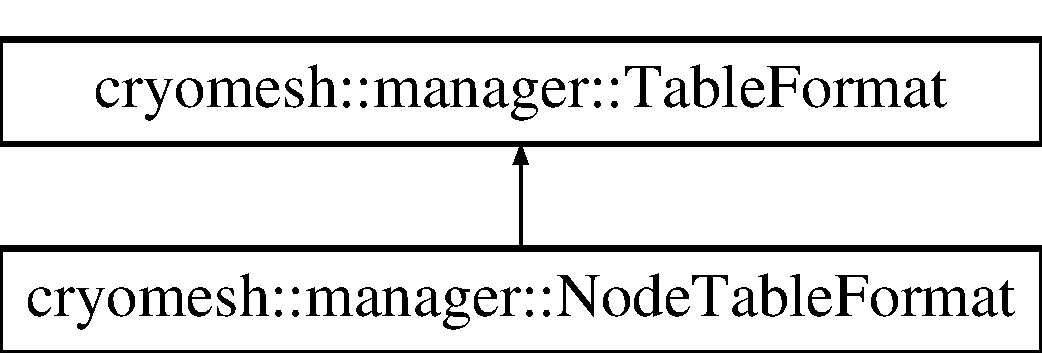
\includegraphics[height=2.000000cm]{structcryomesh_1_1manager_1_1NodeTableFormat}
\end{center}
\end{figure}
\subsection*{\-Public \-Member \-Functions}
\begin{DoxyCompactItemize}
\item 
\hyperlink{structcryomesh_1_1manager_1_1NodeTableFormat_a3fc3590dfb2aaca8658db8f66ca7b5e8}{\-Node\-Table\-Format} ()
\begin{DoxyCompactList}\small\item\em \-Default constructor will construct all the names and columns assiciated with a node table. \end{DoxyCompactList}\item 
std\-::string \hyperlink{structcryomesh_1_1manager_1_1TableFormat_a3e797d6130c6b0745a1fac799c25677a}{get\-Name} () const 
\begin{DoxyCompactList}\small\item\em \-Return the name of the table. \end{DoxyCompactList}\item 
std\-::string \hyperlink{structcryomesh_1_1manager_1_1TableFormat_a2256ce39471582b92bf7cbb6eec74d30}{get\-Key} (const std\-::string \&key)
\begin{DoxyCompactList}\small\item\em \-Return the string object associated with a key. \end{DoxyCompactList}\item 
std\-::string \hyperlink{structcryomesh_1_1manager_1_1TableFormat_a898ae0d0c5490ccdf71aec5156b10fcc}{get\-Create\-Table} () const 
\begin{DoxyCompactList}\small\item\em \-Get the string that can be used to create the sql table. \end{DoxyCompactList}\end{DoxyCompactItemize}
\subsection*{\-Protected \-Attributes}
\begin{DoxyCompactItemize}
\item 
std\-::string \hyperlink{structcryomesh_1_1manager_1_1TableFormat_ab49912897ccb7fd0f8d42f1cc21332e8}{name}
\item 
std\-::map$<$ std\-::string, \*
std\-::string $>$ \hyperlink{structcryomesh_1_1manager_1_1TableFormat_a29ab6f4cfc0c56da1fa461ea665a1b61}{columns}
\end{DoxyCompactItemize}


\subsection{\-Detailed \-Description}
\-Struct representing a node table structure. 

\-Definition at line 99 of file \-Table\-Formats.\-h.



\subsection{\-Constructor \& \-Destructor \-Documentation}
\hypertarget{structcryomesh_1_1manager_1_1NodeTableFormat_a3fc3590dfb2aaca8658db8f66ca7b5e8}{\index{cryomesh\-::manager\-::\-Node\-Table\-Format@{cryomesh\-::manager\-::\-Node\-Table\-Format}!\-Node\-Table\-Format@{\-Node\-Table\-Format}}
\index{\-Node\-Table\-Format@{\-Node\-Table\-Format}!cryomesh::manager::NodeTableFormat@{cryomesh\-::manager\-::\-Node\-Table\-Format}}
\subsubsection[{\-Node\-Table\-Format}]{\setlength{\rightskip}{0pt plus 5cm}{\bf cryomesh\-::manager\-::\-Node\-Table\-Format\-::\-Node\-Table\-Format} (
\begin{DoxyParamCaption}
{}
\end{DoxyParamCaption}
)\hspace{0.3cm}{\ttfamily  \mbox{[}inline\mbox{]}}}}\label{structcryomesh_1_1manager_1_1NodeTableFormat_a3fc3590dfb2aaca8658db8f66ca7b5e8}


\-Default constructor will construct all the names and columns assiciated with a node table. 



\-Definition at line 104 of file \-Table\-Formats.\-h.



\-References cryomesh\-::manager\-::\-Table\-Format\-::columns, and cryomesh\-::manager\-::\-Table\-Format\-::name.



\subsection{\-Member \-Function \-Documentation}
\hypertarget{structcryomesh_1_1manager_1_1TableFormat_a898ae0d0c5490ccdf71aec5156b10fcc}{\index{cryomesh\-::manager\-::\-Node\-Table\-Format@{cryomesh\-::manager\-::\-Node\-Table\-Format}!get\-Create\-Table@{get\-Create\-Table}}
\index{get\-Create\-Table@{get\-Create\-Table}!cryomesh::manager::NodeTableFormat@{cryomesh\-::manager\-::\-Node\-Table\-Format}}
\subsubsection[{get\-Create\-Table}]{\setlength{\rightskip}{0pt plus 5cm}std\-::string {\bf cryomesh\-::manager\-::\-Table\-Format\-::get\-Create\-Table} (
\begin{DoxyParamCaption}
{}
\end{DoxyParamCaption}
) const\hspace{0.3cm}{\ttfamily  \mbox{[}inline, inherited\mbox{]}}}}\label{structcryomesh_1_1manager_1_1TableFormat_a898ae0d0c5490ccdf71aec5156b10fcc}


\-Get the string that can be used to create the sql table. 

\begin{DoxyReturn}{\-Returns}
the sql command string to create this table 
\end{DoxyReturn}


\-Definition at line 60 of file \-Table\-Formats.\-h.



\-References cryomesh\-::manager\-::\-Table\-Format\-::columns, and cryomesh\-::manager\-::\-Table\-Format\-::get\-Name().

\hypertarget{structcryomesh_1_1manager_1_1TableFormat_a2256ce39471582b92bf7cbb6eec74d30}{\index{cryomesh\-::manager\-::\-Node\-Table\-Format@{cryomesh\-::manager\-::\-Node\-Table\-Format}!get\-Key@{get\-Key}}
\index{get\-Key@{get\-Key}!cryomesh::manager::NodeTableFormat@{cryomesh\-::manager\-::\-Node\-Table\-Format}}
\subsubsection[{get\-Key}]{\setlength{\rightskip}{0pt plus 5cm}std\-::string {\bf cryomesh\-::manager\-::\-Table\-Format\-::get\-Key} (
\begin{DoxyParamCaption}
\item[{const std\-::string \&}]{key}
\end{DoxyParamCaption}
)\hspace{0.3cm}{\ttfamily  \mbox{[}inline, inherited\mbox{]}}}}\label{structcryomesh_1_1manager_1_1TableFormat_a2256ce39471582b92bf7cbb6eec74d30}


\-Return the string object associated with a key. 

\-::string \-The key to search for

\begin{DoxyReturn}{\-Returns}
std\-::string \-The object associated with the search key, \char`\"{}\char`\"{} if not found 
\end{DoxyReturn}


\-Definition at line 45 of file \-Table\-Formats.\-h.



\-References cryomesh\-::manager\-::\-Table\-Format\-::columns.

\hypertarget{structcryomesh_1_1manager_1_1TableFormat_a3e797d6130c6b0745a1fac799c25677a}{\index{cryomesh\-::manager\-::\-Node\-Table\-Format@{cryomesh\-::manager\-::\-Node\-Table\-Format}!get\-Name@{get\-Name}}
\index{get\-Name@{get\-Name}!cryomesh::manager::NodeTableFormat@{cryomesh\-::manager\-::\-Node\-Table\-Format}}
\subsubsection[{get\-Name}]{\setlength{\rightskip}{0pt plus 5cm}std\-::string {\bf cryomesh\-::manager\-::\-Table\-Format\-::get\-Name} (
\begin{DoxyParamCaption}
{}
\end{DoxyParamCaption}
) const\hspace{0.3cm}{\ttfamily  \mbox{[}inline, inherited\mbox{]}}}}\label{structcryomesh_1_1manager_1_1TableFormat_a3e797d6130c6b0745a1fac799c25677a}


\-Return the name of the table. 

\begin{DoxyReturn}{\-Returns}
std\-::string \-The name of the table 
\end{DoxyReturn}


\-Definition at line 32 of file \-Table\-Formats.\-h.



\-References cryomesh\-::manager\-::\-Table\-Format\-::name.



\-Referenced by cryomesh\-::manager\-::\-Table\-Format\-::get\-Create\-Table(), cryomesh\-::manager\-::\-Database\-Manager\-::insert\-Connection(), cryomesh\-::manager\-::\-Database\-Manager\-::insert\-Node(), and cryomesh\-::manager\-::\-Database\-Manager\-::insert\-Output\-Pattern().



\subsection{\-Member \-Data \-Documentation}
\hypertarget{structcryomesh_1_1manager_1_1TableFormat_a29ab6f4cfc0c56da1fa461ea665a1b61}{\index{cryomesh\-::manager\-::\-Node\-Table\-Format@{cryomesh\-::manager\-::\-Node\-Table\-Format}!columns@{columns}}
\index{columns@{columns}!cryomesh::manager::NodeTableFormat@{cryomesh\-::manager\-::\-Node\-Table\-Format}}
\subsubsection[{columns}]{\setlength{\rightskip}{0pt plus 5cm}std\-::map$<$std\-::string, std\-::string$>$ {\bf cryomesh\-::manager\-::\-Table\-Format\-::columns}\hspace{0.3cm}{\ttfamily  \mbox{[}protected, inherited\mbox{]}}}}\label{structcryomesh_1_1manager_1_1TableFormat_a29ab6f4cfc0c56da1fa461ea665a1b61}


\-Definition at line 93 of file \-Table\-Formats.\-h.



\-Referenced by cryomesh\-::manager\-::\-Connection\-Table\-Format\-::\-Connection\-Table\-Format(), cryomesh\-::manager\-::\-Table\-Format\-::get\-Create\-Table(), cryomesh\-::manager\-::\-Table\-Format\-::get\-Key(), cryomesh\-::manager\-::\-Input\-Patterns\-Table\-Format\-::\-Input\-Patterns\-Table\-Format(), \-Node\-Table\-Format(), and cryomesh\-::manager\-::\-Output\-Patterns\-Table\-Format\-::\-Output\-Patterns\-Table\-Format().

\hypertarget{structcryomesh_1_1manager_1_1TableFormat_ab49912897ccb7fd0f8d42f1cc21332e8}{\index{cryomesh\-::manager\-::\-Node\-Table\-Format@{cryomesh\-::manager\-::\-Node\-Table\-Format}!name@{name}}
\index{name@{name}!cryomesh::manager::NodeTableFormat@{cryomesh\-::manager\-::\-Node\-Table\-Format}}
\subsubsection[{name}]{\setlength{\rightskip}{0pt plus 5cm}std\-::string {\bf cryomesh\-::manager\-::\-Table\-Format\-::name}\hspace{0.3cm}{\ttfamily  \mbox{[}protected, inherited\mbox{]}}}}\label{structcryomesh_1_1manager_1_1TableFormat_ab49912897ccb7fd0f8d42f1cc21332e8}


\-Definition at line 86 of file \-Table\-Formats.\-h.



\-Referenced by cryomesh\-::manager\-::\-Connection\-Table\-Format\-::\-Connection\-Table\-Format(), cryomesh\-::manager\-::\-Table\-Format\-::get\-Name(), cryomesh\-::manager\-::\-Input\-Patterns\-Table\-Format\-::\-Input\-Patterns\-Table\-Format(), \-Node\-Table\-Format(), and cryomesh\-::manager\-::\-Output\-Patterns\-Table\-Format\-::\-Output\-Patterns\-Table\-Format().



\-The documentation for this struct was generated from the following file\-:\begin{DoxyCompactItemize}
\item 
/home/niall/\-Projects/\-Eclipse/\-C\-P\-P/cryomesh/src/manager/\hyperlink{TableFormats_8h}{\-Table\-Formats.\-h}\end{DoxyCompactItemize}

\hypertarget{structcryomesh_1_1manager_1_1OutputPatternsTableFormat}{\section{cryomesh\-:\-:manager\-:\-:\-Output\-Patterns\-Table\-Format \-Struct \-Reference}
\label{structcryomesh_1_1manager_1_1OutputPatternsTableFormat}\index{cryomesh\-::manager\-::\-Output\-Patterns\-Table\-Format@{cryomesh\-::manager\-::\-Output\-Patterns\-Table\-Format}}
}


\-Struct representing output pattern table structure.  




{\ttfamily \#include $<$\-Table\-Formats.\-h$>$}

\-Inheritance diagram for cryomesh\-:\-:manager\-:\-:\-Output\-Patterns\-Table\-Format\-:\begin{figure}[H]
\begin{center}
\leavevmode
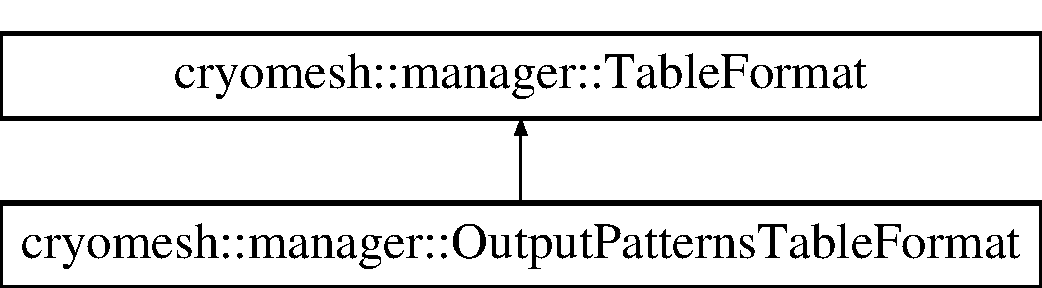
\includegraphics[height=2.000000cm]{structcryomesh_1_1manager_1_1OutputPatternsTableFormat}
\end{center}
\end{figure}
\subsection*{\-Public \-Member \-Functions}
\begin{DoxyCompactItemize}
\item 
\hyperlink{structcryomesh_1_1manager_1_1OutputPatternsTableFormat_af0c661dee8b2943cbb369a2704fccbb9}{\-Output\-Patterns\-Table\-Format} ()
\begin{DoxyCompactList}\small\item\em \-Default constructor will construct all the names and columns assiciated with a pattern table. \end{DoxyCompactList}\item 
std\-::string \hyperlink{structcryomesh_1_1manager_1_1TableFormat_a3e797d6130c6b0745a1fac799c25677a}{get\-Name} () const 
\begin{DoxyCompactList}\small\item\em \-Return the name of the table. \end{DoxyCompactList}\item 
std\-::string \hyperlink{structcryomesh_1_1manager_1_1TableFormat_a2256ce39471582b92bf7cbb6eec74d30}{get\-Key} (const std\-::string \&key)
\begin{DoxyCompactList}\small\item\em \-Return the string object associated with a key. \end{DoxyCompactList}\item 
std\-::string \hyperlink{structcryomesh_1_1manager_1_1TableFormat_a898ae0d0c5490ccdf71aec5156b10fcc}{get\-Create\-Table} () const 
\begin{DoxyCompactList}\small\item\em \-Get the string that can be used to create the sql table. \end{DoxyCompactList}\end{DoxyCompactItemize}
\subsection*{\-Protected \-Attributes}
\begin{DoxyCompactItemize}
\item 
std\-::string \hyperlink{structcryomesh_1_1manager_1_1TableFormat_ab49912897ccb7fd0f8d42f1cc21332e8}{name}
\item 
std\-::map$<$ std\-::string, \*
std\-::string $>$ \hyperlink{structcryomesh_1_1manager_1_1TableFormat_a29ab6f4cfc0c56da1fa461ea665a1b61}{columns}
\end{DoxyCompactItemize}


\subsection{\-Detailed \-Description}
\-Struct representing output pattern table structure. 

\-Definition at line 152 of file \-Table\-Formats.\-h.



\subsection{\-Constructor \& \-Destructor \-Documentation}
\hypertarget{structcryomesh_1_1manager_1_1OutputPatternsTableFormat_af0c661dee8b2943cbb369a2704fccbb9}{\index{cryomesh\-::manager\-::\-Output\-Patterns\-Table\-Format@{cryomesh\-::manager\-::\-Output\-Patterns\-Table\-Format}!\-Output\-Patterns\-Table\-Format@{\-Output\-Patterns\-Table\-Format}}
\index{\-Output\-Patterns\-Table\-Format@{\-Output\-Patterns\-Table\-Format}!cryomesh::manager::OutputPatternsTableFormat@{cryomesh\-::manager\-::\-Output\-Patterns\-Table\-Format}}
\subsubsection[{\-Output\-Patterns\-Table\-Format}]{\setlength{\rightskip}{0pt plus 5cm}{\bf cryomesh\-::manager\-::\-Output\-Patterns\-Table\-Format\-::\-Output\-Patterns\-Table\-Format} (
\begin{DoxyParamCaption}
{}
\end{DoxyParamCaption}
)\hspace{0.3cm}{\ttfamily  \mbox{[}inline\mbox{]}}}}\label{structcryomesh_1_1manager_1_1OutputPatternsTableFormat_af0c661dee8b2943cbb369a2704fccbb9}


\-Default constructor will construct all the names and columns assiciated with a pattern table. 



\-Definition at line 157 of file \-Table\-Formats.\-h.



\-References cryomesh\-::manager\-::\-Table\-Format\-::columns, and cryomesh\-::manager\-::\-Table\-Format\-::name.



\subsection{\-Member \-Function \-Documentation}
\hypertarget{structcryomesh_1_1manager_1_1TableFormat_a898ae0d0c5490ccdf71aec5156b10fcc}{\index{cryomesh\-::manager\-::\-Output\-Patterns\-Table\-Format@{cryomesh\-::manager\-::\-Output\-Patterns\-Table\-Format}!get\-Create\-Table@{get\-Create\-Table}}
\index{get\-Create\-Table@{get\-Create\-Table}!cryomesh::manager::OutputPatternsTableFormat@{cryomesh\-::manager\-::\-Output\-Patterns\-Table\-Format}}
\subsubsection[{get\-Create\-Table}]{\setlength{\rightskip}{0pt plus 5cm}std\-::string {\bf cryomesh\-::manager\-::\-Table\-Format\-::get\-Create\-Table} (
\begin{DoxyParamCaption}
{}
\end{DoxyParamCaption}
) const\hspace{0.3cm}{\ttfamily  \mbox{[}inline, inherited\mbox{]}}}}\label{structcryomesh_1_1manager_1_1TableFormat_a898ae0d0c5490ccdf71aec5156b10fcc}


\-Get the string that can be used to create the sql table. 

\begin{DoxyReturn}{\-Returns}
the sql command string to create this table 
\end{DoxyReturn}


\-Definition at line 60 of file \-Table\-Formats.\-h.



\-References cryomesh\-::manager\-::\-Table\-Format\-::columns, and cryomesh\-::manager\-::\-Table\-Format\-::get\-Name().

\hypertarget{structcryomesh_1_1manager_1_1TableFormat_a2256ce39471582b92bf7cbb6eec74d30}{\index{cryomesh\-::manager\-::\-Output\-Patterns\-Table\-Format@{cryomesh\-::manager\-::\-Output\-Patterns\-Table\-Format}!get\-Key@{get\-Key}}
\index{get\-Key@{get\-Key}!cryomesh::manager::OutputPatternsTableFormat@{cryomesh\-::manager\-::\-Output\-Patterns\-Table\-Format}}
\subsubsection[{get\-Key}]{\setlength{\rightskip}{0pt plus 5cm}std\-::string {\bf cryomesh\-::manager\-::\-Table\-Format\-::get\-Key} (
\begin{DoxyParamCaption}
\item[{const std\-::string \&}]{key}
\end{DoxyParamCaption}
)\hspace{0.3cm}{\ttfamily  \mbox{[}inline, inherited\mbox{]}}}}\label{structcryomesh_1_1manager_1_1TableFormat_a2256ce39471582b92bf7cbb6eec74d30}


\-Return the string object associated with a key. 

\-::string \-The key to search for

\begin{DoxyReturn}{\-Returns}
std\-::string \-The object associated with the search key, \char`\"{}\char`\"{} if not found 
\end{DoxyReturn}


\-Definition at line 45 of file \-Table\-Formats.\-h.



\-References cryomesh\-::manager\-::\-Table\-Format\-::columns.

\hypertarget{structcryomesh_1_1manager_1_1TableFormat_a3e797d6130c6b0745a1fac799c25677a}{\index{cryomesh\-::manager\-::\-Output\-Patterns\-Table\-Format@{cryomesh\-::manager\-::\-Output\-Patterns\-Table\-Format}!get\-Name@{get\-Name}}
\index{get\-Name@{get\-Name}!cryomesh::manager::OutputPatternsTableFormat@{cryomesh\-::manager\-::\-Output\-Patterns\-Table\-Format}}
\subsubsection[{get\-Name}]{\setlength{\rightskip}{0pt plus 5cm}std\-::string {\bf cryomesh\-::manager\-::\-Table\-Format\-::get\-Name} (
\begin{DoxyParamCaption}
{}
\end{DoxyParamCaption}
) const\hspace{0.3cm}{\ttfamily  \mbox{[}inline, inherited\mbox{]}}}}\label{structcryomesh_1_1manager_1_1TableFormat_a3e797d6130c6b0745a1fac799c25677a}


\-Return the name of the table. 

\begin{DoxyReturn}{\-Returns}
std\-::string \-The name of the table 
\end{DoxyReturn}


\-Definition at line 32 of file \-Table\-Formats.\-h.



\-References cryomesh\-::manager\-::\-Table\-Format\-::name.



\-Referenced by cryomesh\-::manager\-::\-Table\-Format\-::get\-Create\-Table(), cryomesh\-::manager\-::\-Database\-Manager\-::insert\-Connection(), cryomesh\-::manager\-::\-Database\-Manager\-::insert\-Node(), and cryomesh\-::manager\-::\-Database\-Manager\-::insert\-Output\-Pattern().



\subsection{\-Member \-Data \-Documentation}
\hypertarget{structcryomesh_1_1manager_1_1TableFormat_a29ab6f4cfc0c56da1fa461ea665a1b61}{\index{cryomesh\-::manager\-::\-Output\-Patterns\-Table\-Format@{cryomesh\-::manager\-::\-Output\-Patterns\-Table\-Format}!columns@{columns}}
\index{columns@{columns}!cryomesh::manager::OutputPatternsTableFormat@{cryomesh\-::manager\-::\-Output\-Patterns\-Table\-Format}}
\subsubsection[{columns}]{\setlength{\rightskip}{0pt plus 5cm}std\-::map$<$std\-::string, std\-::string$>$ {\bf cryomesh\-::manager\-::\-Table\-Format\-::columns}\hspace{0.3cm}{\ttfamily  \mbox{[}protected, inherited\mbox{]}}}}\label{structcryomesh_1_1manager_1_1TableFormat_a29ab6f4cfc0c56da1fa461ea665a1b61}


\-Definition at line 93 of file \-Table\-Formats.\-h.



\-Referenced by cryomesh\-::manager\-::\-Connection\-Table\-Format\-::\-Connection\-Table\-Format(), cryomesh\-::manager\-::\-Table\-Format\-::get\-Create\-Table(), cryomesh\-::manager\-::\-Table\-Format\-::get\-Key(), cryomesh\-::manager\-::\-Input\-Patterns\-Table\-Format\-::\-Input\-Patterns\-Table\-Format(), cryomesh\-::manager\-::\-Node\-Table\-Format\-::\-Node\-Table\-Format(), and \-Output\-Patterns\-Table\-Format().

\hypertarget{structcryomesh_1_1manager_1_1TableFormat_ab49912897ccb7fd0f8d42f1cc21332e8}{\index{cryomesh\-::manager\-::\-Output\-Patterns\-Table\-Format@{cryomesh\-::manager\-::\-Output\-Patterns\-Table\-Format}!name@{name}}
\index{name@{name}!cryomesh::manager::OutputPatternsTableFormat@{cryomesh\-::manager\-::\-Output\-Patterns\-Table\-Format}}
\subsubsection[{name}]{\setlength{\rightskip}{0pt plus 5cm}std\-::string {\bf cryomesh\-::manager\-::\-Table\-Format\-::name}\hspace{0.3cm}{\ttfamily  \mbox{[}protected, inherited\mbox{]}}}}\label{structcryomesh_1_1manager_1_1TableFormat_ab49912897ccb7fd0f8d42f1cc21332e8}


\-Definition at line 86 of file \-Table\-Formats.\-h.



\-Referenced by cryomesh\-::manager\-::\-Connection\-Table\-Format\-::\-Connection\-Table\-Format(), cryomesh\-::manager\-::\-Table\-Format\-::get\-Name(), cryomesh\-::manager\-::\-Input\-Patterns\-Table\-Format\-::\-Input\-Patterns\-Table\-Format(), cryomesh\-::manager\-::\-Node\-Table\-Format\-::\-Node\-Table\-Format(), and \-Output\-Patterns\-Table\-Format().



\-The documentation for this struct was generated from the following file\-:\begin{DoxyCompactItemize}
\item 
/home/niall/\-Projects/\-Eclipse/\-C\-P\-P/cryomesh/src/manager/\hyperlink{TableFormats_8h}{\-Table\-Formats.\-h}\end{DoxyCompactItemize}

\hypertarget{classcryomesh_1_1state_1_1Pattern}{\section{cryomesh\-:\-:state\-:\-:\-Pattern \-Class \-Reference}
\label{classcryomesh_1_1state_1_1Pattern}\index{cryomesh\-::state\-::\-Pattern@{cryomesh\-::state\-::\-Pattern}}
}


{\ttfamily \#include $<$\-Pattern.\-h$>$}

\subsection*{\-Public \-Member \-Functions}
\begin{DoxyCompactItemize}
\item 
\hyperlink{classcryomesh_1_1state_1_1Pattern_a5e9e2738edae7cd79164b834e1cdee6c}{\-Pattern} ()
\item 
\hyperlink{classcryomesh_1_1state_1_1Pattern_a40fda07d27a5ced7e527fbd48d3e908c}{\-Pattern} (const \hyperlink{classcryomesh_1_1state_1_1Pattern}{\-Pattern} \&)
\item 
\hyperlink{classcryomesh_1_1state_1_1Pattern_a2c4fa08b8a29111c2c3d037d5ef294a5}{\-Pattern} (const std\-::string \&)
\item 
\hyperlink{classcryomesh_1_1state_1_1Pattern_ad90e47bde0cc1163799853af58a3558c}{\-Pattern} (const std\-::vector$<$ bool $>$ \&)
\item 
\hyperlink{classcryomesh_1_1state_1_1Pattern_a8a1d2344caa2e6b15465a0e6b50c78ab}{\-Pattern} (const \hyperlink{classcryomesh_1_1state_1_1BinaryString}{\-Binary\-String} \&obj)
\item 
virtual \hyperlink{classcryomesh_1_1state_1_1Pattern_a6fd2a03ab3ee83afb5925b5eca5475e2}{$\sim$\-Pattern} ()
\item 
\hyperlink{classcryomesh_1_1state_1_1Pattern}{\-Pattern} \& \hyperlink{classcryomesh_1_1state_1_1Pattern_ae160b228aff3b4bcc49792588b2fbee6}{operator=} (const \hyperlink{classcryomesh_1_1state_1_1Pattern}{\-Pattern} \&)
\item 
double \hyperlink{classcryomesh_1_1state_1_1Pattern_ad6f8afd23c5eaeb585d5690496d81c05}{compare} (const \hyperlink{classcryomesh_1_1state_1_1Pattern}{\-Pattern} \&) const 
\item 
bool \hyperlink{classcryomesh_1_1state_1_1Pattern_a8dc6809b00c16358f993ac7e774d130a}{is\-All\-Zeroes} () const 
\item 
bool \hyperlink{classcryomesh_1_1state_1_1Pattern_a4a9f45cfa7eec822e011b49036436369}{operator==} (const \hyperlink{classcryomesh_1_1state_1_1Pattern}{\-Pattern} \&) const 
\item 
bool \hyperlink{classcryomesh_1_1state_1_1Pattern_ad3fb10247785d26c3cf150f7e69df35a}{operator$<$} (const \hyperlink{classcryomesh_1_1state_1_1Pattern}{\-Pattern} \&) const 
\item 
std\-::vector$<$ bool $>$ \hyperlink{classcryomesh_1_1state_1_1Pattern_ab6fe1d9bee48f3bdaffb0cf683de4d17}{get\-Pattern} () const 
\item 
std\-::string \hyperlink{classcryomesh_1_1state_1_1Pattern_a963b252435300f16df7599c56751555b}{get\-String} () const 
\item 
void \hyperlink{classcryomesh_1_1state_1_1Pattern_acf193a66c3a2e41d99f40b2666687ad9}{set\-Pattern} (const std\-::vector$<$ bool $>$ \&)
\item 
int \hyperlink{classcryomesh_1_1state_1_1Pattern_a34597e6294ffb843326b654991aceb2f}{get\-Id} () const 
\item 
void \hyperlink{classcryomesh_1_1state_1_1Pattern_a8ca895dafdf58ae592f41be1d8d6173a}{set\-Id} (int)
\item 
int \hyperlink{classcryomesh_1_1state_1_1Pattern_a77793823c718ec5bacf59d3908950390}{get\-Width} () const 
\item 
int \hyperlink{classcryomesh_1_1state_1_1Pattern_a448d14d09a39d35182bef8169511faf8}{get\-Size} () const 
\item 
const \hyperlink{classcryomesh_1_1state_1_1BinaryString}{\-Binary\-String} \& \hyperlink{classcryomesh_1_1state_1_1Pattern_a57b18a4b690c70821e7d84847a56d7b9}{get\-Binary\-String} () const 
\item 
\hyperlink{classcryomesh_1_1state_1_1BinaryString}{\-Binary\-String} \& \hyperlink{classcryomesh_1_1state_1_1Pattern_a22e7fa5faa704b0d95c022d1dc5d67aa}{get\-Mutable\-Binary\-String} ()
\item 
const boost\-::shared\-\_\-ptr\*
$<$ \hyperlink{classcryomesh_1_1state_1_1PatternTag}{\-Pattern\-Tag} $>$ \hyperlink{classcryomesh_1_1state_1_1Pattern_aec6c5defbc96290f03a2178bbd08a626}{get\-Pattern\-Tag} () const 
\item 
void \hyperlink{classcryomesh_1_1state_1_1Pattern_afae212fb317cf86e70ee93b9a0c6ea21}{set\-Pattern\-Tag} (boost\-::shared\-\_\-ptr$<$ \hyperlink{classcryomesh_1_1state_1_1PatternTag}{\-Pattern\-Tag} $>$ pt)
\item 
boost\-::shared\-\_\-ptr\*
$<$ \hyperlink{classcryomesh_1_1manager_1_1DatabaseObject}{manager\-::\-Database\-Object} $>$ \hyperlink{classcryomesh_1_1state_1_1Pattern_a2dd3aa753f926b674aa73688a932ebf7}{get\-Database\-Object} () const 
\end{DoxyCompactItemize}
\subsection*{\-Static \-Public \-Member \-Functions}
\begin{DoxyCompactItemize}
\item 
static int \hyperlink{classcryomesh_1_1state_1_1Pattern_aaf0fef8e434a2bf4e2a3de2146506e55}{get\-Ids} ()
\item 
static int \hyperlink{classcryomesh_1_1state_1_1Pattern_a02fe1e3bc02dad188199408748aa8e76}{assign\-Ids} ()
\item 
static void \hyperlink{classcryomesh_1_1state_1_1Pattern_abe885f1239abb58a449d945d02513599}{set\-Ids} (int)
\item 
static std\-::string \hyperlink{classcryomesh_1_1state_1_1Pattern_a8b72b4b8c76445cf788129ed5b6b42a5}{pattern\-To\-String} (const std\-::vector$<$ bool $>$ \&vec)
\item 
static std\-::vector$<$ bool $>$ \hyperlink{classcryomesh_1_1state_1_1Pattern_a30238bc06f4cbf29d28adff1fd09b280}{string\-To\-Pattern} (const std\-::string \&)
\item 
static \hyperlink{classcryomesh_1_1state_1_1Pattern}{\-Pattern} \hyperlink{classcryomesh_1_1state_1_1Pattern_ad253bf9c3cb1997ce2f8db2ded5455ba}{get\-Random} (unsigned int width, double fraction=0.\-5)
\begin{DoxyCompactList}\small\item\em \-Generate a random pattern of width. \end{DoxyCompactList}\end{DoxyCompactItemize}
\subsection*{\-Private \-Member \-Functions}
\begin{DoxyCompactItemize}
\item 
{\footnotesize template$<$class Archive $>$ }\\void \hyperlink{classcryomesh_1_1state_1_1Pattern_afe08a220604e76d3f01156783303eee6}{serialize} (\-Archive \&ar, const unsigned int version)
\item 
void \hyperlink{classcryomesh_1_1state_1_1Pattern_a5488a0554ecbcf4749ce79f5523972d9}{initialise} ()
\end{DoxyCompactItemize}
\subsection*{\-Private \-Attributes}
\begin{DoxyCompactItemize}
\item 
\hyperlink{classcryomesh_1_1state_1_1BinaryString}{\-Binary\-String} \hyperlink{classcryomesh_1_1state_1_1Pattern_a2ceffaffb21669b4712f9af5f5045e6e}{binary\-String}
\item 
int \hyperlink{classcryomesh_1_1state_1_1Pattern_aa8070cf7c7e5621164fcf389baeec552}{id}
\item 
boost\-::shared\-\_\-ptr$<$ \hyperlink{classcryomesh_1_1state_1_1PatternTag}{\-Pattern\-Tag} $>$ \hyperlink{classcryomesh_1_1state_1_1Pattern_ae6138b7407f2e55de84a1c53fcc14a35}{pattern\-Tag}
\end{DoxyCompactItemize}
\subsection*{\-Static \-Private \-Attributes}
\begin{DoxyCompactItemize}
\item 
static int \hyperlink{classcryomesh_1_1state_1_1Pattern_a9a1488a4d6c293a0c5c5517fbcb47cb7}{ids} = 1
\end{DoxyCompactItemize}
\subsection*{\-Friends}
\begin{DoxyCompactItemize}
\item 
class \hyperlink{classcryomesh_1_1state_1_1Pattern_ac98d07dd8f7b70e16ccb9a01abf56b9c}{boost\-::serialization\-::access}
\item 
std\-::ostream \& \hyperlink{classcryomesh_1_1state_1_1Pattern_aade38e7e420a07b60712bd1891487f23}{operator$<$$<$} (std\-::ostream \&os, const \hyperlink{classcryomesh_1_1state_1_1Pattern}{\-Pattern} \&obj)
\end{DoxyCompactItemize}


\subsection{\-Detailed \-Description}


\-Definition at line 27 of file \-Pattern.\-h.



\subsection{\-Constructor \& \-Destructor \-Documentation}
\hypertarget{classcryomesh_1_1state_1_1Pattern_a5e9e2738edae7cd79164b834e1cdee6c}{\index{cryomesh\-::state\-::\-Pattern@{cryomesh\-::state\-::\-Pattern}!\-Pattern@{\-Pattern}}
\index{\-Pattern@{\-Pattern}!cryomesh::state::Pattern@{cryomesh\-::state\-::\-Pattern}}
\subsubsection[{\-Pattern}]{\setlength{\rightskip}{0pt plus 5cm}{\bf cryomesh\-::state\-::\-Pattern\-::\-Pattern} (
\begin{DoxyParamCaption}
{}
\end{DoxyParamCaption}
)}}\label{classcryomesh_1_1state_1_1Pattern_a5e9e2738edae7cd79164b834e1cdee6c}


\-Definition at line 31 of file \-Pattern.\-cpp.



\-References initialise().



\-Referenced by get\-Random().

\hypertarget{classcryomesh_1_1state_1_1Pattern_a40fda07d27a5ced7e527fbd48d3e908c}{\index{cryomesh\-::state\-::\-Pattern@{cryomesh\-::state\-::\-Pattern}!\-Pattern@{\-Pattern}}
\index{\-Pattern@{\-Pattern}!cryomesh::state::Pattern@{cryomesh\-::state\-::\-Pattern}}
\subsubsection[{\-Pattern}]{\setlength{\rightskip}{0pt plus 5cm}{\bf cryomesh\-::state\-::\-Pattern\-::\-Pattern} (
\begin{DoxyParamCaption}
\item[{const {\bf \-Pattern} \&}]{pat}
\end{DoxyParamCaption}
)}}\label{classcryomesh_1_1state_1_1Pattern_a40fda07d27a5ced7e527fbd48d3e908c}


\-Definition at line 35 of file \-Pattern.\-cpp.



\-References initialise().

\hypertarget{classcryomesh_1_1state_1_1Pattern_a2c4fa08b8a29111c2c3d037d5ef294a5}{\index{cryomesh\-::state\-::\-Pattern@{cryomesh\-::state\-::\-Pattern}!\-Pattern@{\-Pattern}}
\index{\-Pattern@{\-Pattern}!cryomesh::state::Pattern@{cryomesh\-::state\-::\-Pattern}}
\subsubsection[{\-Pattern}]{\setlength{\rightskip}{0pt plus 5cm}{\bf cryomesh\-::state\-::\-Pattern\-::\-Pattern} (
\begin{DoxyParamCaption}
\item[{const std\-::string \&}]{str}
\end{DoxyParamCaption}
)}}\label{classcryomesh_1_1state_1_1Pattern_a2c4fa08b8a29111c2c3d037d5ef294a5}


\-Definition at line 43 of file \-Pattern.\-cpp.



\-References initialise().

\hypertarget{classcryomesh_1_1state_1_1Pattern_ad90e47bde0cc1163799853af58a3558c}{\index{cryomesh\-::state\-::\-Pattern@{cryomesh\-::state\-::\-Pattern}!\-Pattern@{\-Pattern}}
\index{\-Pattern@{\-Pattern}!cryomesh::state::Pattern@{cryomesh\-::state\-::\-Pattern}}
\subsubsection[{\-Pattern}]{\setlength{\rightskip}{0pt plus 5cm}{\bf cryomesh\-::state\-::\-Pattern\-::\-Pattern} (
\begin{DoxyParamCaption}
\item[{const std\-::vector$<$ bool $>$ \&}]{pat}
\end{DoxyParamCaption}
)}}\label{classcryomesh_1_1state_1_1Pattern_ad90e47bde0cc1163799853af58a3558c}


\-Definition at line 39 of file \-Pattern.\-cpp.



\-References initialise().

\hypertarget{classcryomesh_1_1state_1_1Pattern_a8a1d2344caa2e6b15465a0e6b50c78ab}{\index{cryomesh\-::state\-::\-Pattern@{cryomesh\-::state\-::\-Pattern}!\-Pattern@{\-Pattern}}
\index{\-Pattern@{\-Pattern}!cryomesh::state::Pattern@{cryomesh\-::state\-::\-Pattern}}
\subsubsection[{\-Pattern}]{\setlength{\rightskip}{0pt plus 5cm}{\bf cryomesh\-::state\-::\-Pattern\-::\-Pattern} (
\begin{DoxyParamCaption}
\item[{const {\bf \-Binary\-String} \&}]{obj}
\end{DoxyParamCaption}
)}}\label{classcryomesh_1_1state_1_1Pattern_a8a1d2344caa2e6b15465a0e6b50c78ab}
\hypertarget{classcryomesh_1_1state_1_1Pattern_a6fd2a03ab3ee83afb5925b5eca5475e2}{\index{cryomesh\-::state\-::\-Pattern@{cryomesh\-::state\-::\-Pattern}!$\sim$\-Pattern@{$\sim$\-Pattern}}
\index{$\sim$\-Pattern@{$\sim$\-Pattern}!cryomesh::state::Pattern@{cryomesh\-::state\-::\-Pattern}}
\subsubsection[{$\sim$\-Pattern}]{\setlength{\rightskip}{0pt plus 5cm}{\bf cryomesh\-::state\-::\-Pattern\-::$\sim$\-Pattern} (
\begin{DoxyParamCaption}
{}
\end{DoxyParamCaption}
)\hspace{0.3cm}{\ttfamily  \mbox{[}virtual\mbox{]}}}}\label{classcryomesh_1_1state_1_1Pattern_a6fd2a03ab3ee83afb5925b5eca5475e2}


\-Definition at line 47 of file \-Pattern.\-cpp.



\subsection{\-Member \-Function \-Documentation}
\hypertarget{classcryomesh_1_1state_1_1Pattern_a02fe1e3bc02dad188199408748aa8e76}{\index{cryomesh\-::state\-::\-Pattern@{cryomesh\-::state\-::\-Pattern}!assign\-Ids@{assign\-Ids}}
\index{assign\-Ids@{assign\-Ids}!cryomesh::state::Pattern@{cryomesh\-::state\-::\-Pattern}}
\subsubsection[{assign\-Ids}]{\setlength{\rightskip}{0pt plus 5cm}int {\bf cryomesh\-::state\-::\-Pattern\-::assign\-Ids} (
\begin{DoxyParamCaption}
{}
\end{DoxyParamCaption}
)\hspace{0.3cm}{\ttfamily  \mbox{[}static\mbox{]}}}}\label{classcryomesh_1_1state_1_1Pattern_a02fe1e3bc02dad188199408748aa8e76}


\-Definition at line 212 of file \-Pattern.\-cpp.



\-References ids.

\hypertarget{classcryomesh_1_1state_1_1Pattern_ad6f8afd23c5eaeb585d5690496d81c05}{\index{cryomesh\-::state\-::\-Pattern@{cryomesh\-::state\-::\-Pattern}!compare@{compare}}
\index{compare@{compare}!cryomesh::state::Pattern@{cryomesh\-::state\-::\-Pattern}}
\subsubsection[{compare}]{\setlength{\rightskip}{0pt plus 5cm}double {\bf cryomesh\-::state\-::\-Pattern\-::compare} (
\begin{DoxyParamCaption}
\item[{const {\bf \-Pattern} \&}]{obj}
\end{DoxyParamCaption}
) const}}\label{classcryomesh_1_1state_1_1Pattern_ad6f8afd23c5eaeb585d5690496d81c05}


\-Definition at line 63 of file \-Pattern.\-cpp.



\-References get\-Pattern().

\hypertarget{classcryomesh_1_1state_1_1Pattern_a57b18a4b690c70821e7d84847a56d7b9}{\index{cryomesh\-::state\-::\-Pattern@{cryomesh\-::state\-::\-Pattern}!get\-Binary\-String@{get\-Binary\-String}}
\index{get\-Binary\-String@{get\-Binary\-String}!cryomesh::state::Pattern@{cryomesh\-::state\-::\-Pattern}}
\subsubsection[{get\-Binary\-String}]{\setlength{\rightskip}{0pt plus 5cm}const {\bf \-Binary\-String} \& {\bf cryomesh\-::state\-::\-Pattern\-::get\-Binary\-String} (
\begin{DoxyParamCaption}
{}
\end{DoxyParamCaption}
) const}}\label{classcryomesh_1_1state_1_1Pattern_a57b18a4b690c70821e7d84847a56d7b9}


\-Definition at line 159 of file \-Pattern.\-cpp.



\-References binary\-String.



\-Referenced by operator=().

\hypertarget{classcryomesh_1_1state_1_1Pattern_a2dd3aa753f926b674aa73688a932ebf7}{\index{cryomesh\-::state\-::\-Pattern@{cryomesh\-::state\-::\-Pattern}!get\-Database\-Object@{get\-Database\-Object}}
\index{get\-Database\-Object@{get\-Database\-Object}!cryomesh::state::Pattern@{cryomesh\-::state\-::\-Pattern}}
\subsubsection[{get\-Database\-Object}]{\setlength{\rightskip}{0pt plus 5cm}boost\-::shared\-\_\-ptr$<$ {\bf manager\-::\-Database\-Object} $>$ {\bf cryomesh\-::state\-::\-Pattern\-::get\-Database\-Object} (
\begin{DoxyParamCaption}
{}
\end{DoxyParamCaption}
) const}}\label{classcryomesh_1_1state_1_1Pattern_a2dd3aa753f926b674aa73688a932ebf7}


\-Definition at line 229 of file \-Pattern.\-cpp.



\-References cryomesh\-::common\-::\-Time\-Keeper\-::get\-Cycle(), get\-String(), cryomesh\-::common\-::\-Time\-Keeper\-::get\-Time\-Keeper(), and cryomesh\-::common\-::\-Cycle\-::to\-U\-L\-Int().

\hypertarget{classcryomesh_1_1state_1_1Pattern_a34597e6294ffb843326b654991aceb2f}{\index{cryomesh\-::state\-::\-Pattern@{cryomesh\-::state\-::\-Pattern}!get\-Id@{get\-Id}}
\index{get\-Id@{get\-Id}!cryomesh::state::Pattern@{cryomesh\-::state\-::\-Pattern}}
\subsubsection[{get\-Id}]{\setlength{\rightskip}{0pt plus 5cm}int {\bf cryomesh\-::state\-::\-Pattern\-::get\-Id} (
\begin{DoxyParamCaption}
{}
\end{DoxyParamCaption}
) const}}\label{classcryomesh_1_1state_1_1Pattern_a34597e6294ffb843326b654991aceb2f}


\-Definition at line 142 of file \-Pattern.\-cpp.



\-References id.



\-Referenced by operator$<$(), cryomesh\-::state\-::operator$<$$<$(), and operator=().

\hypertarget{classcryomesh_1_1state_1_1Pattern_aaf0fef8e434a2bf4e2a3de2146506e55}{\index{cryomesh\-::state\-::\-Pattern@{cryomesh\-::state\-::\-Pattern}!get\-Ids@{get\-Ids}}
\index{get\-Ids@{get\-Ids}!cryomesh::state::Pattern@{cryomesh\-::state\-::\-Pattern}}
\subsubsection[{get\-Ids}]{\setlength{\rightskip}{0pt plus 5cm}int {\bf cryomesh\-::state\-::\-Pattern\-::get\-Ids} (
\begin{DoxyParamCaption}
{}
\end{DoxyParamCaption}
)\hspace{0.3cm}{\ttfamily  \mbox{[}static\mbox{]}}}}\label{classcryomesh_1_1state_1_1Pattern_aaf0fef8e434a2bf4e2a3de2146506e55}


\-Definition at line 218 of file \-Pattern.\-cpp.



\-References ids.



\-Referenced by cryomesh\-::state\-::\-Pattern\-Tag\-By\-Id\-::get\-End\-Tag().

\hypertarget{classcryomesh_1_1state_1_1Pattern_a22e7fa5faa704b0d95c022d1dc5d67aa}{\index{cryomesh\-::state\-::\-Pattern@{cryomesh\-::state\-::\-Pattern}!get\-Mutable\-Binary\-String@{get\-Mutable\-Binary\-String}}
\index{get\-Mutable\-Binary\-String@{get\-Mutable\-Binary\-String}!cryomesh::state::Pattern@{cryomesh\-::state\-::\-Pattern}}
\subsubsection[{get\-Mutable\-Binary\-String}]{\setlength{\rightskip}{0pt plus 5cm}{\bf \-Binary\-String} \& {\bf cryomesh\-::state\-::\-Pattern\-::get\-Mutable\-Binary\-String} (
\begin{DoxyParamCaption}
{}
\end{DoxyParamCaption}
)}}\label{classcryomesh_1_1state_1_1Pattern_a22e7fa5faa704b0d95c022d1dc5d67aa}


\-Definition at line 162 of file \-Pattern.\-cpp.



\-References binary\-String.

\hypertarget{classcryomesh_1_1state_1_1Pattern_ab6fe1d9bee48f3bdaffb0cf683de4d17}{\index{cryomesh\-::state\-::\-Pattern@{cryomesh\-::state\-::\-Pattern}!get\-Pattern@{get\-Pattern}}
\index{get\-Pattern@{get\-Pattern}!cryomesh::state::Pattern@{cryomesh\-::state\-::\-Pattern}}
\subsubsection[{get\-Pattern}]{\setlength{\rightskip}{0pt plus 5cm}std\-::vector$<$ bool $>$ {\bf cryomesh\-::state\-::\-Pattern\-::get\-Pattern} (
\begin{DoxyParamCaption}
{}
\end{DoxyParamCaption}
) const}}\label{classcryomesh_1_1state_1_1Pattern_ab6fe1d9bee48f3bdaffb0cf683de4d17}


\-Definition at line 133 of file \-Pattern.\-cpp.



\-References binary\-String, and cryomesh\-::state\-::\-Binary\-String\-::get\-Bools().



\-Referenced by compare(), cryomesh\-::structures\-::\-Fibre\-::force\-Fire\-Nodes(), get\-String(), operator==(), and cryomesh\-::structures\-::\-Fibre\-::trigger().

\hypertarget{classcryomesh_1_1state_1_1Pattern_aec6c5defbc96290f03a2178bbd08a626}{\index{cryomesh\-::state\-::\-Pattern@{cryomesh\-::state\-::\-Pattern}!get\-Pattern\-Tag@{get\-Pattern\-Tag}}
\index{get\-Pattern\-Tag@{get\-Pattern\-Tag}!cryomesh::state::Pattern@{cryomesh\-::state\-::\-Pattern}}
\subsubsection[{get\-Pattern\-Tag}]{\setlength{\rightskip}{0pt plus 5cm}const boost\-::shared\-\_\-ptr$<$ {\bf \-Pattern\-Tag} $>$ {\bf cryomesh\-::state\-::\-Pattern\-::get\-Pattern\-Tag} (
\begin{DoxyParamCaption}
{}
\end{DoxyParamCaption}
) const}}\label{classcryomesh_1_1state_1_1Pattern_aec6c5defbc96290f03a2178bbd08a626}


\-Definition at line 205 of file \-Pattern.\-cpp.



\-References pattern\-Tag.

\hypertarget{classcryomesh_1_1state_1_1Pattern_ad253bf9c3cb1997ce2f8db2ded5455ba}{\index{cryomesh\-::state\-::\-Pattern@{cryomesh\-::state\-::\-Pattern}!get\-Random@{get\-Random}}
\index{get\-Random@{get\-Random}!cryomesh::state::Pattern@{cryomesh\-::state\-::\-Pattern}}
\subsubsection[{get\-Random}]{\setlength{\rightskip}{0pt plus 5cm}{\bf \-Pattern} {\bf cryomesh\-::state\-::\-Pattern\-::get\-Random} (
\begin{DoxyParamCaption}
\item[{unsigned int}]{width, }
\item[{double}]{fraction = {\ttfamily 0.5}}
\end{DoxyParamCaption}
)\hspace{0.3cm}{\ttfamily  \mbox{[}static\mbox{]}}}}\label{classcryomesh_1_1state_1_1Pattern_ad253bf9c3cb1997ce2f8db2ded5455ba}


\-Generate a random pattern of width. 


\begin{DoxyParams}{\-Parameters}
{\em unsigned} & int \-Width of pattern to generate \\
\hline
{\em double} & \-Fraction of pattern to activate, default to 0.\-5 \\
\hline
\end{DoxyParams}
\begin{DoxyReturn}{\-Returns}
\hyperlink{classcryomesh_1_1state_1_1Pattern}{\-Pattern} \-The random pattern 
\end{DoxyReturn}


\-Definition at line 21 of file \-Pattern.\-cpp.



\-References \-Pattern().



\-Referenced by cryomesh\-::structures\-::\-Fibre\-::trigger().

\hypertarget{classcryomesh_1_1state_1_1Pattern_a448d14d09a39d35182bef8169511faf8}{\index{cryomesh\-::state\-::\-Pattern@{cryomesh\-::state\-::\-Pattern}!get\-Size@{get\-Size}}
\index{get\-Size@{get\-Size}!cryomesh::state::Pattern@{cryomesh\-::state\-::\-Pattern}}
\subsubsection[{get\-Size}]{\setlength{\rightskip}{0pt plus 5cm}int {\bf cryomesh\-::state\-::\-Pattern\-::get\-Size} (
\begin{DoxyParamCaption}
{}
\end{DoxyParamCaption}
) const}}\label{classcryomesh_1_1state_1_1Pattern_a448d14d09a39d35182bef8169511faf8}


\-Definition at line 155 of file \-Pattern.\-cpp.



\-References binary\-String, and cryomesh\-::state\-::\-Binary\-String\-::get\-Width().



\-Referenced by cryomesh\-::structures\-::\-Fibre\-::force\-Fire\-Nodes(), and get\-Width().

\hypertarget{classcryomesh_1_1state_1_1Pattern_a963b252435300f16df7599c56751555b}{\index{cryomesh\-::state\-::\-Pattern@{cryomesh\-::state\-::\-Pattern}!get\-String@{get\-String}}
\index{get\-String@{get\-String}!cryomesh::state::Pattern@{cryomesh\-::state\-::\-Pattern}}
\subsubsection[{get\-String}]{\setlength{\rightskip}{0pt plus 5cm}std\-::string {\bf cryomesh\-::state\-::\-Pattern\-::get\-String} (
\begin{DoxyParamCaption}
{}
\end{DoxyParamCaption}
) const}}\label{classcryomesh_1_1state_1_1Pattern_a963b252435300f16df7599c56751555b}


\-Definition at line 136 of file \-Pattern.\-cpp.



\-References get\-Pattern(), and pattern\-To\-String().



\-Referenced by get\-Database\-Object(), and cryomesh\-::state\-::operator$<$$<$().

\hypertarget{classcryomesh_1_1state_1_1Pattern_a77793823c718ec5bacf59d3908950390}{\index{cryomesh\-::state\-::\-Pattern@{cryomesh\-::state\-::\-Pattern}!get\-Width@{get\-Width}}
\index{get\-Width@{get\-Width}!cryomesh::state::Pattern@{cryomesh\-::state\-::\-Pattern}}
\subsubsection[{get\-Width}]{\setlength{\rightskip}{0pt plus 5cm}int {\bf cryomesh\-::state\-::\-Pattern\-::get\-Width} (
\begin{DoxyParamCaption}
{}
\end{DoxyParamCaption}
) const}}\label{classcryomesh_1_1state_1_1Pattern_a77793823c718ec5bacf59d3908950390}


\-Definition at line 151 of file \-Pattern.\-cpp.



\-References get\-Size().

\hypertarget{classcryomesh_1_1state_1_1Pattern_a5488a0554ecbcf4749ce79f5523972d9}{\index{cryomesh\-::state\-::\-Pattern@{cryomesh\-::state\-::\-Pattern}!initialise@{initialise}}
\index{initialise@{initialise}!cryomesh::state::Pattern@{cryomesh\-::state\-::\-Pattern}}
\subsubsection[{initialise}]{\setlength{\rightskip}{0pt plus 5cm}void {\bf cryomesh\-::state\-::\-Pattern\-::initialise} (
\begin{DoxyParamCaption}
{}
\end{DoxyParamCaption}
)\hspace{0.3cm}{\ttfamily  \mbox{[}private\mbox{]}}}}\label{classcryomesh_1_1state_1_1Pattern_a5488a0554ecbcf4749ce79f5523972d9}


\-Definition at line 237 of file \-Pattern.\-cpp.



\-References pattern\-Tag.



\-Referenced by operator=(), and \-Pattern().

\hypertarget{classcryomesh_1_1state_1_1Pattern_a8dc6809b00c16358f993ac7e774d130a}{\index{cryomesh\-::state\-::\-Pattern@{cryomesh\-::state\-::\-Pattern}!is\-All\-Zeroes@{is\-All\-Zeroes}}
\index{is\-All\-Zeroes@{is\-All\-Zeroes}!cryomesh::state::Pattern@{cryomesh\-::state\-::\-Pattern}}
\subsubsection[{is\-All\-Zeroes}]{\setlength{\rightskip}{0pt plus 5cm}bool {\bf cryomesh\-::state\-::\-Pattern\-::is\-All\-Zeroes} (
\begin{DoxyParamCaption}
{}
\end{DoxyParamCaption}
) const}}\label{classcryomesh_1_1state_1_1Pattern_a8dc6809b00c16358f993ac7e774d130a}


\-Definition at line 60 of file \-Pattern.\-cpp.



\-References binary\-String, and cryomesh\-::state\-::\-Binary\-String\-::is\-All\-Zeroes().

\hypertarget{classcryomesh_1_1state_1_1Pattern_ad3fb10247785d26c3cf150f7e69df35a}{\index{cryomesh\-::state\-::\-Pattern@{cryomesh\-::state\-::\-Pattern}!operator$<$@{operator$<$}}
\index{operator$<$@{operator$<$}!cryomesh::state::Pattern@{cryomesh\-::state\-::\-Pattern}}
\subsubsection[{operator$<$}]{\setlength{\rightskip}{0pt plus 5cm}bool cryomesh\-::state\-::\-Pattern\-::operator$<$ (
\begin{DoxyParamCaption}
\item[{const {\bf \-Pattern} \&}]{obj}
\end{DoxyParamCaption}
) const}}\label{classcryomesh_1_1state_1_1Pattern_ad3fb10247785d26c3cf150f7e69df35a}


\-Definition at line 129 of file \-Pattern.\-cpp.



\-References get\-Id().

\hypertarget{classcryomesh_1_1state_1_1Pattern_ae160b228aff3b4bcc49792588b2fbee6}{\index{cryomesh\-::state\-::\-Pattern@{cryomesh\-::state\-::\-Pattern}!operator=@{operator=}}
\index{operator=@{operator=}!cryomesh::state::Pattern@{cryomesh\-::state\-::\-Pattern}}
\subsubsection[{operator=}]{\setlength{\rightskip}{0pt plus 5cm}{\bf \-Pattern} \& cryomesh\-::state\-::\-Pattern\-::operator= (
\begin{DoxyParamCaption}
\item[{const {\bf \-Pattern} \&}]{obj}
\end{DoxyParamCaption}
)}}\label{classcryomesh_1_1state_1_1Pattern_ae160b228aff3b4bcc49792588b2fbee6}


\-Definition at line 51 of file \-Pattern.\-cpp.



\-References binary\-String, get\-Binary\-String(), get\-Id(), initialise(), and set\-Id().

\hypertarget{classcryomesh_1_1state_1_1Pattern_a4a9f45cfa7eec822e011b49036436369}{\index{cryomesh\-::state\-::\-Pattern@{cryomesh\-::state\-::\-Pattern}!operator==@{operator==}}
\index{operator==@{operator==}!cryomesh::state::Pattern@{cryomesh\-::state\-::\-Pattern}}
\subsubsection[{operator==}]{\setlength{\rightskip}{0pt plus 5cm}bool cryomesh\-::state\-::\-Pattern\-::operator== (
\begin{DoxyParamCaption}
\item[{const {\bf \-Pattern} \&}]{obj}
\end{DoxyParamCaption}
) const}}\label{classcryomesh_1_1state_1_1Pattern_a4a9f45cfa7eec822e011b49036436369}


\-Definition at line 115 of file \-Pattern.\-cpp.



\-References get\-Pattern().

\hypertarget{classcryomesh_1_1state_1_1Pattern_a8b72b4b8c76445cf788129ed5b6b42a5}{\index{cryomesh\-::state\-::\-Pattern@{cryomesh\-::state\-::\-Pattern}!pattern\-To\-String@{pattern\-To\-String}}
\index{pattern\-To\-String@{pattern\-To\-String}!cryomesh::state::Pattern@{cryomesh\-::state\-::\-Pattern}}
\subsubsection[{pattern\-To\-String}]{\setlength{\rightskip}{0pt plus 5cm}std\-::string {\bf cryomesh\-::state\-::\-Pattern\-::pattern\-To\-String} (
\begin{DoxyParamCaption}
\item[{const std\-::vector$<$ bool $>$ \&}]{vec}
\end{DoxyParamCaption}
)\hspace{0.3cm}{\ttfamily  \mbox{[}static\mbox{]}}}}\label{classcryomesh_1_1state_1_1Pattern_a8b72b4b8c76445cf788129ed5b6b42a5}


\-Definition at line 166 of file \-Pattern.\-cpp.



\-Referenced by get\-String().

\hypertarget{classcryomesh_1_1state_1_1Pattern_afe08a220604e76d3f01156783303eee6}{\index{cryomesh\-::state\-::\-Pattern@{cryomesh\-::state\-::\-Pattern}!serialize@{serialize}}
\index{serialize@{serialize}!cryomesh::state::Pattern@{cryomesh\-::state\-::\-Pattern}}
\subsubsection[{serialize}]{\setlength{\rightskip}{0pt plus 5cm}template$<$class Archive $>$ void {\bf cryomesh\-::state\-::\-Pattern\-::serialize} (
\begin{DoxyParamCaption}
\item[{\-Archive \&}]{ar, }
\item[{const unsigned int}]{version}
\end{DoxyParamCaption}
)\hspace{0.3cm}{\ttfamily  \mbox{[}inline, private\mbox{]}}}}\label{classcryomesh_1_1state_1_1Pattern_afe08a220604e76d3f01156783303eee6}


\-Definition at line 30 of file \-Pattern.\-h.



\-References binary\-String, id, and ids.

\hypertarget{classcryomesh_1_1state_1_1Pattern_a8ca895dafdf58ae592f41be1d8d6173a}{\index{cryomesh\-::state\-::\-Pattern@{cryomesh\-::state\-::\-Pattern}!set\-Id@{set\-Id}}
\index{set\-Id@{set\-Id}!cryomesh::state::Pattern@{cryomesh\-::state\-::\-Pattern}}
\subsubsection[{set\-Id}]{\setlength{\rightskip}{0pt plus 5cm}void {\bf cryomesh\-::state\-::\-Pattern\-::set\-Id} (
\begin{DoxyParamCaption}
\item[{int}]{new\-\_\-id}
\end{DoxyParamCaption}
)}}\label{classcryomesh_1_1state_1_1Pattern_a8ca895dafdf58ae592f41be1d8d6173a}


\-Definition at line 145 of file \-Pattern.\-cpp.



\-Referenced by operator=().

\hypertarget{classcryomesh_1_1state_1_1Pattern_abe885f1239abb58a449d945d02513599}{\index{cryomesh\-::state\-::\-Pattern@{cryomesh\-::state\-::\-Pattern}!set\-Ids@{set\-Ids}}
\index{set\-Ids@{set\-Ids}!cryomesh::state::Pattern@{cryomesh\-::state\-::\-Pattern}}
\subsubsection[{set\-Ids}]{\setlength{\rightskip}{0pt plus 5cm}void {\bf cryomesh\-::state\-::\-Pattern\-::set\-Ids} (
\begin{DoxyParamCaption}
\item[{int}]{is}
\end{DoxyParamCaption}
)\hspace{0.3cm}{\ttfamily  \mbox{[}static\mbox{]}}}}\label{classcryomesh_1_1state_1_1Pattern_abe885f1239abb58a449d945d02513599}


\-Definition at line 222 of file \-Pattern.\-cpp.



\-References ids.

\hypertarget{classcryomesh_1_1state_1_1Pattern_acf193a66c3a2e41d99f40b2666687ad9}{\index{cryomesh\-::state\-::\-Pattern@{cryomesh\-::state\-::\-Pattern}!set\-Pattern@{set\-Pattern}}
\index{set\-Pattern@{set\-Pattern}!cryomesh::state::Pattern@{cryomesh\-::state\-::\-Pattern}}
\subsubsection[{set\-Pattern}]{\setlength{\rightskip}{0pt plus 5cm}void {\bf cryomesh\-::state\-::\-Pattern\-::set\-Pattern} (
\begin{DoxyParamCaption}
\item[{const std\-::vector$<$ bool $>$ \&}]{pat}
\end{DoxyParamCaption}
)}}\label{classcryomesh_1_1state_1_1Pattern_acf193a66c3a2e41d99f40b2666687ad9}


\-Definition at line 139 of file \-Pattern.\-cpp.



\-References binary\-String, and cryomesh\-::state\-::\-Binary\-String\-::set\-Binary\-String().

\hypertarget{classcryomesh_1_1state_1_1Pattern_afae212fb317cf86e70ee93b9a0c6ea21}{\index{cryomesh\-::state\-::\-Pattern@{cryomesh\-::state\-::\-Pattern}!set\-Pattern\-Tag@{set\-Pattern\-Tag}}
\index{set\-Pattern\-Tag@{set\-Pattern\-Tag}!cryomesh::state::Pattern@{cryomesh\-::state\-::\-Pattern}}
\subsubsection[{set\-Pattern\-Tag}]{\setlength{\rightskip}{0pt plus 5cm}void {\bf cryomesh\-::state\-::\-Pattern\-::set\-Pattern\-Tag} (
\begin{DoxyParamCaption}
\item[{boost\-::shared\-\_\-ptr$<$ {\bf \-Pattern\-Tag} $>$}]{pt}
\end{DoxyParamCaption}
)}}\label{classcryomesh_1_1state_1_1Pattern_afae212fb317cf86e70ee93b9a0c6ea21}


\-Definition at line 208 of file \-Pattern.\-cpp.



\-References pattern\-Tag.

\hypertarget{classcryomesh_1_1state_1_1Pattern_a30238bc06f4cbf29d28adff1fd09b280}{\index{cryomesh\-::state\-::\-Pattern@{cryomesh\-::state\-::\-Pattern}!string\-To\-Pattern@{string\-To\-Pattern}}
\index{string\-To\-Pattern@{string\-To\-Pattern}!cryomesh::state::Pattern@{cryomesh\-::state\-::\-Pattern}}
\subsubsection[{string\-To\-Pattern}]{\setlength{\rightskip}{0pt plus 5cm}std\-::vector$<$ bool $>$ {\bf cryomesh\-::state\-::\-Pattern\-::string\-To\-Pattern} (
\begin{DoxyParamCaption}
\item[{const std\-::string \&}]{str}
\end{DoxyParamCaption}
)\hspace{0.3cm}{\ttfamily  \mbox{[}static\mbox{]}}}}\label{classcryomesh_1_1state_1_1Pattern_a30238bc06f4cbf29d28adff1fd09b280}


\-Definition at line 184 of file \-Pattern.\-cpp.



\subsection{\-Friends \-And \-Related \-Function \-Documentation}
\hypertarget{classcryomesh_1_1state_1_1Pattern_ac98d07dd8f7b70e16ccb9a01abf56b9c}{\index{cryomesh\-::state\-::\-Pattern@{cryomesh\-::state\-::\-Pattern}!boost\-::serialization\-::access@{boost\-::serialization\-::access}}
\index{boost\-::serialization\-::access@{boost\-::serialization\-::access}!cryomesh::state::Pattern@{cryomesh\-::state\-::\-Pattern}}
\subsubsection[{boost\-::serialization\-::access}]{\setlength{\rightskip}{0pt plus 5cm}friend class boost\-::serialization\-::access\hspace{0.3cm}{\ttfamily  \mbox{[}friend\mbox{]}}}}\label{classcryomesh_1_1state_1_1Pattern_ac98d07dd8f7b70e16ccb9a01abf56b9c}


\-Definition at line 28 of file \-Pattern.\-h.

\hypertarget{classcryomesh_1_1state_1_1Pattern_aade38e7e420a07b60712bd1891487f23}{\index{cryomesh\-::state\-::\-Pattern@{cryomesh\-::state\-::\-Pattern}!operator$<$$<$@{operator$<$$<$}}
\index{operator$<$$<$@{operator$<$$<$}!cryomesh::state::Pattern@{cryomesh\-::state\-::\-Pattern}}
\subsubsection[{operator$<$$<$}]{\setlength{\rightskip}{0pt plus 5cm}std\-::ostream\& operator$<$$<$ (
\begin{DoxyParamCaption}
\item[{std\-::ostream \&}]{os, }
\item[{const {\bf \-Pattern} \&}]{obj}
\end{DoxyParamCaption}
)\hspace{0.3cm}{\ttfamily  \mbox{[}friend\mbox{]}}}}\label{classcryomesh_1_1state_1_1Pattern_aade38e7e420a07b60712bd1891487f23}


\-Definition at line 242 of file \-Pattern.\-cpp.



\subsection{\-Member \-Data \-Documentation}
\hypertarget{classcryomesh_1_1state_1_1Pattern_a2ceffaffb21669b4712f9af5f5045e6e}{\index{cryomesh\-::state\-::\-Pattern@{cryomesh\-::state\-::\-Pattern}!binary\-String@{binary\-String}}
\index{binary\-String@{binary\-String}!cryomesh::state::Pattern@{cryomesh\-::state\-::\-Pattern}}
\subsubsection[{binary\-String}]{\setlength{\rightskip}{0pt plus 5cm}{\bf \-Binary\-String} {\bf cryomesh\-::state\-::\-Pattern\-::binary\-String}\hspace{0.3cm}{\ttfamily  \mbox{[}private\mbox{]}}}}\label{classcryomesh_1_1state_1_1Pattern_a2ceffaffb21669b4712f9af5f5045e6e}


\-Definition at line 115 of file \-Pattern.\-h.



\-Referenced by get\-Binary\-String(), get\-Mutable\-Binary\-String(), get\-Pattern(), get\-Size(), is\-All\-Zeroes(), operator=(), serialize(), and set\-Pattern().

\hypertarget{classcryomesh_1_1state_1_1Pattern_aa8070cf7c7e5621164fcf389baeec552}{\index{cryomesh\-::state\-::\-Pattern@{cryomesh\-::state\-::\-Pattern}!id@{id}}
\index{id@{id}!cryomesh::state::Pattern@{cryomesh\-::state\-::\-Pattern}}
\subsubsection[{id}]{\setlength{\rightskip}{0pt plus 5cm}int {\bf cryomesh\-::state\-::\-Pattern\-::id}\hspace{0.3cm}{\ttfamily  \mbox{[}private\mbox{]}}}}\label{classcryomesh_1_1state_1_1Pattern_aa8070cf7c7e5621164fcf389baeec552}


\-Definition at line 117 of file \-Pattern.\-h.



\-Referenced by get\-Id(), and serialize().

\hypertarget{classcryomesh_1_1state_1_1Pattern_a9a1488a4d6c293a0c5c5517fbcb47cb7}{\index{cryomesh\-::state\-::\-Pattern@{cryomesh\-::state\-::\-Pattern}!ids@{ids}}
\index{ids@{ids}!cryomesh::state::Pattern@{cryomesh\-::state\-::\-Pattern}}
\subsubsection[{ids}]{\setlength{\rightskip}{0pt plus 5cm}int {\bf cryomesh\-::state\-::\-Pattern\-::ids} = 1\hspace{0.3cm}{\ttfamily  \mbox{[}static, private\mbox{]}}}}\label{classcryomesh_1_1state_1_1Pattern_a9a1488a4d6c293a0c5c5517fbcb47cb7}


\-Definition at line 128 of file \-Pattern.\-h.



\-Referenced by assign\-Ids(), get\-Ids(), serialize(), and set\-Ids().

\hypertarget{classcryomesh_1_1state_1_1Pattern_ae6138b7407f2e55de84a1c53fcc14a35}{\index{cryomesh\-::state\-::\-Pattern@{cryomesh\-::state\-::\-Pattern}!pattern\-Tag@{pattern\-Tag}}
\index{pattern\-Tag@{pattern\-Tag}!cryomesh::state::Pattern@{cryomesh\-::state\-::\-Pattern}}
\subsubsection[{pattern\-Tag}]{\setlength{\rightskip}{0pt plus 5cm}boost\-::shared\-\_\-ptr$<${\bf \-Pattern\-Tag}$>$ {\bf cryomesh\-::state\-::\-Pattern\-::pattern\-Tag}\hspace{0.3cm}{\ttfamily  \mbox{[}private\mbox{]}}}}\label{classcryomesh_1_1state_1_1Pattern_ae6138b7407f2e55de84a1c53fcc14a35}


\-Definition at line 120 of file \-Pattern.\-h.



\-Referenced by get\-Pattern\-Tag(), initialise(), and set\-Pattern\-Tag().



\-The documentation for this class was generated from the following files\-:\begin{DoxyCompactItemize}
\item 
/home/niall/\-Projects/\-Eclipse/\-C\-P\-P/cryomesh/src/state/\hyperlink{Pattern_8h}{\-Pattern.\-h}\item 
/home/niall/\-Projects/\-Eclipse/\-C\-P\-P/cryomesh/src/state/\hyperlink{Pattern_8cpp}{\-Pattern.\-cpp}\end{DoxyCompactItemize}

\hypertarget{classcryomesh_1_1state_1_1PatternChannel}{\section{cryomesh\-:\-:state\-:\-:\-Pattern\-Channel \-Class \-Reference}
\label{classcryomesh_1_1state_1_1PatternChannel}\index{cryomesh\-::state\-::\-Pattern\-Channel@{cryomesh\-::state\-::\-Pattern\-Channel}}
}


{\ttfamily \#include $<$\-Pattern\-Channel.\-h$>$}

\subsection*{\-Public \-Types}
\begin{DoxyCompactItemize}
\item 
enum \hyperlink{classcryomesh_1_1state_1_1PatternChannel_aecb6feb12b771abb3cca4a77f5a47903}{\-Print\-Format} \{ \hyperlink{classcryomesh_1_1state_1_1PatternChannel_aecb6feb12b771abb3cca4a77f5a47903ac9ab380f74b4a50f13013e4785cf9e41}{\-B\-I\-N\-A\-R\-Y}, 
\hyperlink{classcryomesh_1_1state_1_1PatternChannel_aecb6feb12b771abb3cca4a77f5a47903a323e9e3c328769d1ef777f10b3a2315b}{\-T\-E\-X\-T}, 
\hyperlink{classcryomesh_1_1state_1_1PatternChannel_aecb6feb12b771abb3cca4a77f5a47903a95004c9c6007ed3c766a5e6cec3ed521}{\-I\-N\-T\-E\-G\-E\-R}
 \}
\item 
enum \hyperlink{classcryomesh_1_1state_1_1PatternChannel_ac8a0ae515a221519890fc1181f2c895a}{\-Channel\-Data\-Type} \{ \hyperlink{classcryomesh_1_1state_1_1PatternChannel_ac8a0ae515a221519890fc1181f2c895aab75202b529e4a7cfb8db3daa14b9f477}{\-Input}, 
\hyperlink{classcryomesh_1_1state_1_1PatternChannel_ac8a0ae515a221519890fc1181f2c895aa981b9873565a0888e43eef95b4d003bf}{\-Output}, 
\hyperlink{classcryomesh_1_1state_1_1PatternChannel_ac8a0ae515a221519890fc1181f2c895aa4f561e33e002f951204ee1f01497f994}{\-Transitional}
 \}
\end{DoxyCompactItemize}
\subsection*{\-Public \-Member \-Functions}
\begin{DoxyCompactItemize}
\item 
\hyperlink{classcryomesh_1_1state_1_1PatternChannel_a10d5404f3c3d7005d48f681552cca552}{\-Pattern\-Channel} (\hyperlink{classcryomesh_1_1state_1_1PatternChannel_ac8a0ae515a221519890fc1181f2c895a}{\-Channel\-Data\-Type} dt)
\item 
\hyperlink{classcryomesh_1_1state_1_1PatternChannel_a15701153fd6de84797aee5b6543e90ec}{\-Pattern\-Channel} (const std\-::list$<$ boost\-::shared\-\_\-ptr$<$ \hyperlink{classcryomesh_1_1state_1_1Pattern}{\-Pattern} $>$ $>$ \&pats, \hyperlink{classcryomesh_1_1state_1_1PatternChannel_ac8a0ae515a221519890fc1181f2c895a}{\-Channel\-Data\-Type} dt)
\item 
virtual \hyperlink{classcryomesh_1_1state_1_1PatternChannel_ad2f8eaa8b1925a9bab61181154511b51}{$\sim$\-Pattern\-Channel} ()
\item 
\hyperlink{classcryomesh_1_1state_1_1PatternChannel_a840ee854b5050c4034de97ee7625a562}{\-Pattern\-Channel} (const \hyperlink{classcryomesh_1_1state_1_1PatternChannel}{\-Pattern\-Channel} \&obj)
\item 
\hyperlink{classcryomesh_1_1state_1_1PatternChannel}{\-Pattern\-Channel} \& \hyperlink{classcryomesh_1_1state_1_1PatternChannel_a136a8a320b095ad9ce04eb67ea0a8c17}{operator=} (const \hyperlink{classcryomesh_1_1state_1_1PatternChannel}{\-Pattern\-Channel} \&obj)
\begin{DoxyCompactList}\small\item\em \-Assignment operator. \end{DoxyCompactList}\item 
void \hyperlink{classcryomesh_1_1state_1_1PatternChannel_ab8c96531bfdfa24facbec91e81fa0158}{add\-Pattern} (boost\-::shared\-\_\-ptr$<$ \hyperlink{classcryomesh_1_1state_1_1Pattern}{\-Pattern} $>$ pat)
\item 
void \hyperlink{classcryomesh_1_1state_1_1PatternChannel_a46b385352284ab06ea31c36bfb37a0ac}{add\-Patterns} (const std\-::list$<$ boost\-::shared\-\_\-ptr$<$ \hyperlink{classcryomesh_1_1state_1_1Pattern}{\-Pattern} $>$ $>$ \&pats)
\item 
void \hyperlink{classcryomesh_1_1state_1_1PatternChannel_a79780e5a353cd0e376d0a8abad93f8bd}{add\-Patterns} (const std\-::list$<$ boost\-::shared\-\_\-ptr$<$ \hyperlink{classcryomesh_1_1state_1_1Pattern}{\-Pattern} $>$ $>$ \&pats, int position)
\item 
std\-::list$<$ boost\-::shared\-\_\-ptr\*
$<$ \hyperlink{classcryomesh_1_1state_1_1Pattern}{\-Pattern} $>$ $>$ \hyperlink{classcryomesh_1_1state_1_1PatternChannel_a58645e5bd3b44290db489c095ad34895}{remove\-Patterns} (const std\-::list$<$ boost\-::shared\-\_\-ptr$<$ \hyperlink{classcryomesh_1_1state_1_1Pattern}{\-Pattern} $>$ $>$ \&pats)
\item 
std\-::list$<$ boost\-::shared\-\_\-ptr\*
$<$ \hyperlink{classcryomesh_1_1state_1_1Pattern}{\-Pattern} $>$ $>$ \hyperlink{classcryomesh_1_1state_1_1PatternChannel_a95cdc1ef47d4647f16db7a618fbcb1c3}{remove\-Patterns} (const std\-::list$<$ boost\-::uuids\-::uuid $>$ \&uuids)
\item 
void \hyperlink{classcryomesh_1_1state_1_1PatternChannel_a13753c86675493e5cb8cb911238e3410}{clear\-Pattern\-List} ()
\item 
std\-::list$<$ boost\-::shared\-\_\-ptr\*
$<$ \hyperlink{classcryomesh_1_1state_1_1Pattern}{\-Pattern} $>$ $>$ \hyperlink{classcryomesh_1_1state_1_1PatternChannel_a756aafbdf9bd37870b60ae1e5c174c27}{force\-Pattern\-List\-Size} (int sz)
\item 
std\-::list$<$ boost\-::shared\-\_\-ptr\*
$<$ \hyperlink{classcryomesh_1_1state_1_1Pattern}{\-Pattern} $>$ $>$ \hyperlink{classcryomesh_1_1state_1_1PatternChannel_a66783001791bd4b51bec7eb97b8a1b4e}{force\-Pattern\-List\-Size} ()
\item 
const boost\-::shared\-\_\-ptr$<$ \hyperlink{classcryomesh_1_1state_1_1Pattern}{\-Pattern} $>$ \hyperlink{classcryomesh_1_1state_1_1PatternChannel_a92ef0469e782dc022c00d804f30fff3d}{get\-Current\-Pattern} ()
\item 
const boost\-::shared\-\_\-ptr$<$ \hyperlink{classcryomesh_1_1state_1_1Pattern}{\-Pattern} $>$ \hyperlink{classcryomesh_1_1state_1_1PatternChannel_a553a85437f3197ea4fa751319de0fd56}{get\-Pattern\-By\-Cycle} (const \hyperlink{classcryomesh_1_1common_1_1Cycle}{common\-::\-Cycle} \&cycle)
\item 
const boost\-::shared\-\_\-ptr$<$ \hyperlink{classcryomesh_1_1state_1_1Pattern}{\-Pattern} $>$ \hyperlink{classcryomesh_1_1state_1_1PatternChannel_a88e0394f678b199aa5f2866b1487fc92}{get\-Pattern\-By\-Tag} (const boost\-::shared\-\_\-ptr$<$ \hyperlink{classcryomesh_1_1state_1_1PatternTag}{\-Pattern\-Tag} $>$ tg) const 
\item 
const boost\-::shared\-\_\-ptr$<$ \hyperlink{classcryomesh_1_1state_1_1Pattern}{\-Pattern} $>$ \hyperlink{classcryomesh_1_1state_1_1PatternChannel_ae5dd9fdcebe6af92c48c4ac1f0d889c7}{next\-Pattern} ()
\item 
const boost\-::shared\-\_\-ptr$<$ \hyperlink{classcryomesh_1_1state_1_1Pattern}{\-Pattern} $>$ \hyperlink{classcryomesh_1_1state_1_1PatternChannel_a4b96871d0a8bf38d6d9a2998dd0a81f7}{previous\-Pattern} ()
\item 
double \hyperlink{classcryomesh_1_1state_1_1PatternChannel_a05400d50d8206b82426bdc8b277c4c14}{match\-Globally} (const \hyperlink{classcryomesh_1_1state_1_1PatternChannel}{\-Pattern\-Channel} \&)
\item 
double \hyperlink{classcryomesh_1_1state_1_1PatternChannel_aa354fc22d88359c3b83d92a224761c69}{match\-Sequentially} (const \hyperlink{classcryomesh_1_1state_1_1PatternChannel}{\-Pattern\-Channel} \&)
\item 
virtual void \hyperlink{classcryomesh_1_1state_1_1PatternChannel_acbaa7ae7afbe42e8ebca56f889220289}{enable\-Debug} (bool b)
\item 
\hyperlink{classcryomesh_1_1state_1_1PatternChannel_ac8a0ae515a221519890fc1181f2c895a}{\-Channel\-Data\-Type} \hyperlink{classcryomesh_1_1state_1_1PatternChannel_ad7890be8253221b14e673c4fb1cddffa}{get\-Channel\-Data\-Type} () const 
\item 
int \hyperlink{classcryomesh_1_1state_1_1PatternChannel_a7ab7d66118f678d1406a14c4ebb79752}{get\-Length} () const 
\item 
const std\-::map\*
$<$ boost\-::shared\-\_\-ptr\*
$<$ \hyperlink{classcryomesh_1_1state_1_1PatternTag}{\-Pattern\-Tag} $>$\*
, boost\-::uuids\-::uuid $>$ \& \hyperlink{classcryomesh_1_1state_1_1PatternChannel_ab5260edbf3ada707a91994c60b866dd5}{get\-Pattern\-By\-Tag\-Map} () const 
\item 
const boost\-::shared\-\_\-ptr$<$ \hyperlink{classcryomesh_1_1state_1_1Pattern}{\-Pattern} $>$ \hyperlink{classcryomesh_1_1state_1_1PatternChannel_a33b3c30b6137eaf727a58cafab32f692}{get\-Pattern\-By\-U\-U\-I\-D} (const boost\-::uuids\-::uuid \&id) const 
\item 
boost\-::shared\-\_\-ptr$<$ \hyperlink{classcryomesh_1_1state_1_1Pattern}{\-Pattern} $>$ \hyperlink{classcryomesh_1_1state_1_1PatternChannel_ad588e65dc12cee6d91bb3035a6958d44}{get\-Mutable\-Pattern\-By\-U\-U\-I\-D} (const boost\-::uuids\-::uuid \&id)
\item 
const std\-::list\*
$<$ boost\-::uuids\-::uuid $>$ \& \hyperlink{classcryomesh_1_1state_1_1PatternChannel_a56b0b495e91692302da543807a93fa02}{get\-Pattern\-List} () const 
\item 
std\-::list$<$ boost\-::uuids\-::uuid $>$\*
\-::iterator \hyperlink{classcryomesh_1_1state_1_1PatternChannel_a79af2f63fa3b5dfa7c48615a47c20842}{get\-Pattern\-List\-Iterator} () const 
\item 
const std\-::map\*
$<$ boost\-::uuids\-::uuid, \*
boost\-::shared\-\_\-ptr$<$ \hyperlink{classcryomesh_1_1state_1_1Pattern}{\-Pattern} $>$ $>$ \& \hyperlink{classcryomesh_1_1state_1_1PatternChannel_ab3bc796775ce23366a18206ac2c5119d}{get\-Pattern\-Map} () const 
\item 
int \hyperlink{classcryomesh_1_1state_1_1PatternChannel_a930bbb05180ecd22aa9a87eb62daba0f}{get\-Pattern\-Position} () const 
\item 
int \hyperlink{classcryomesh_1_1state_1_1PatternChannel_a1b02b011f6abc75354e75fe44218190d}{get\-Width} () const 
\item 
void \hyperlink{classcryomesh_1_1state_1_1PatternChannel_ae9f396f25c1f9650cc57b4c02c84a5f3}{set\-Width} (int w)
\item 
int \hyperlink{classcryomesh_1_1state_1_1PatternChannel_a6d02f9db85383449d208ebb012edbe48}{get\-Ref\-I\-D} () const 
\item 
void \hyperlink{classcryomesh_1_1state_1_1PatternChannel_a8df9a6aace2cf6810d3d6f3bc72b5a3b}{set\-Ref\-I\-D} (int r)
\item 
int \hyperlink{classcryomesh_1_1state_1_1PatternChannel_a6c1ae5242c32abd71055d35c7d126bfa}{get\-Max\-Pattern\-List\-Size} () const 
\item 
void \hyperlink{classcryomesh_1_1state_1_1PatternChannel_acd69920f539ac7a7149faa92c5e766e1}{set\-Max\-Pattern\-List\-Size} (int sz)
\item 
std\-::ostream \& \hyperlink{classcryomesh_1_1state_1_1PatternChannel_a74a37c66904647c83d459ee4a90446d7}{print\-Pattern\-List} (std\-::ostream \&os, bool reversed=false) const 
\item 
std\-::ostream \& \hyperlink{classcryomesh_1_1state_1_1PatternChannel_a1ab67f8d6565a4a2b987152d4c38d175}{print\-Text\-Formatted\-Pattern\-List} (std\-::ostream \&os, bool reversed=false) const 
\item 
std\-::ostream \& \hyperlink{classcryomesh_1_1state_1_1PatternChannel_a8d92b898f11a8cea38022bf888807c69}{print\-Integer\-Formatted\-Pattern\-List} (std\-::ostream \&os, bool reversed) const 
\item 
std\-::ostream \& \hyperlink{classcryomesh_1_1state_1_1PatternChannel_aa6d23443589ea223baed8eb9042a2139}{print\-Binary\-Formatted\-Pattern\-List} (std\-::ostream \&os, bool reversed) const 
\item 
std\-::ostream \& \hyperlink{classcryomesh_1_1state_1_1PatternChannel_a4813e35ef5321611b83d523c5cc3bfb6}{print\-Formatted\-Pattern\-List} (std\-::ostream \&os, const \hyperlink{classcryomesh_1_1state_1_1PatternChannel_aecb6feb12b771abb3cca4a77f5a47903}{\-Print\-Format} \&pf, bool reversed) const 
\end{DoxyCompactItemize}
\subsection*{\-Static \-Public \-Member \-Functions}
\begin{DoxyCompactItemize}
\item 
static unsigned int \hyperlink{classcryomesh_1_1state_1_1PatternChannel_a4a1ca89d0b7867c4faa13d779a35ae97}{get\-Ref\-I\-D\-S} ()
\end{DoxyCompactItemize}
\subsection*{\-Static \-Public \-Attributes}
\begin{DoxyCompactItemize}
\item 
static const int \hyperlink{classcryomesh_1_1state_1_1PatternChannel_a2931ca38ca2e5d816c8917cb857e62fc}{\-D\-E\-F\-A\-U\-L\-T\-\_\-\-M\-A\-X\-\_\-\-P\-A\-T\-T\-E\-R\-N\-\_\-\-L\-I\-S\-T\-\_\-\-S\-I\-Z\-E} = -\/1
\item 
static const unsigned int \hyperlink{classcryomesh_1_1state_1_1PatternChannel_a1476695074d7d8e184aed0c4401f72d5}{\-R\-E\-F\-I\-D\-\_\-\-C\-R\-E\-A\-T\-E\-\_\-\-S\-T\-A\-R\-T} = 100000
\item 
static unsigned int \hyperlink{classcryomesh_1_1state_1_1PatternChannel_aafed47c54c1db97487a333f43bb85e25}{ref\-I\-D\-S} = \hyperlink{classcryomesh_1_1state_1_1PatternChannel_a1476695074d7d8e184aed0c4401f72d5}{\-Pattern\-Channel\-::\-R\-E\-F\-I\-D\-\_\-\-C\-R\-E\-A\-T\-E\-\_\-\-S\-T\-A\-R\-T}
\end{DoxyCompactItemize}
\subsection*{\-Private \-Attributes}
\begin{DoxyCompactItemize}
\item 
\hyperlink{classcryomesh_1_1state_1_1PatternChannel_ac8a0ae515a221519890fc1181f2c895a}{\-Channel\-Data\-Type} \hyperlink{classcryomesh_1_1state_1_1PatternChannel_a0638a69625dd19480563b245dc1c6853}{channel\-Data\-Type}
\item 
int \hyperlink{classcryomesh_1_1state_1_1PatternChannel_a979af8e9743379cc8484cfa7348838f2}{length}
\item 
int \hyperlink{classcryomesh_1_1state_1_1PatternChannel_aeab8770881ec9be1b48c712a23dd6271}{max\-Pattern\-List\-Size}
\item 
std\-::map$<$ boost\-::shared\-\_\-ptr\*
$<$ \hyperlink{classcryomesh_1_1state_1_1PatternTag}{\-Pattern\-Tag} $>$\*
, boost\-::uuids\-::uuid $>$ \hyperlink{classcryomesh_1_1state_1_1PatternChannel_a5155045e7e94fc10a1d60e418bf82b71}{pattern\-By\-Tag\-Map}
\item 
std\-::list$<$ boost\-::uuids\-::uuid $>$ \hyperlink{classcryomesh_1_1state_1_1PatternChannel_a71800edd10923b7b00f0c292414b4ba1}{pattern\-List}
\item 
std\-::list$<$ boost\-::uuids\-::uuid $>$\*
\-::iterator \hyperlink{classcryomesh_1_1state_1_1PatternChannel_ac06b2bd5e0bc4aa4da633bc80a64b290}{pattern\-List\-Iterator}
\item 
std\-::map$<$ boost\-::uuids\-::uuid, \*
boost\-::shared\-\_\-ptr$<$ \hyperlink{classcryomesh_1_1state_1_1Pattern}{\-Pattern} $>$ $>$ \hyperlink{classcryomesh_1_1state_1_1PatternChannel_a72f70fbaad5ff134b07c3fe198d9fd67}{pattern\-Map}
\item 
int \hyperlink{classcryomesh_1_1state_1_1PatternChannel_af4a9ce80cd65ae8a11ec27e4b027a34c}{pattern\-Position}
\item 
int \hyperlink{classcryomesh_1_1state_1_1PatternChannel_a609d1d8ac76ff856bf7885c040dc339a}{ref\-I\-D}
\item 
int \hyperlink{classcryomesh_1_1state_1_1PatternChannel_af7bcede6cf5c8d768e7d1f1d897106d2}{width}
\end{DoxyCompactItemize}
\subsection*{\-Friends}
\begin{DoxyCompactItemize}
\item 
std\-::ostream \& \hyperlink{classcryomesh_1_1state_1_1PatternChannel_a8a4a6cb06dd05aa353207980bcf59319}{operator$<$$<$} (std\-::ostream \&os, const \hyperlink{classcryomesh_1_1state_1_1PatternChannel}{\-Pattern\-Channel} \&obj)
\end{DoxyCompactItemize}


\subsection{\-Detailed \-Description}


\-Definition at line 25 of file \-Pattern\-Channel.\-h.



\subsection{\-Member \-Enumeration \-Documentation}
\hypertarget{classcryomesh_1_1state_1_1PatternChannel_ac8a0ae515a221519890fc1181f2c895a}{\index{cryomesh\-::state\-::\-Pattern\-Channel@{cryomesh\-::state\-::\-Pattern\-Channel}!\-Channel\-Data\-Type@{\-Channel\-Data\-Type}}
\index{\-Channel\-Data\-Type@{\-Channel\-Data\-Type}!cryomesh::state::PatternChannel@{cryomesh\-::state\-::\-Pattern\-Channel}}
\subsubsection[{\-Channel\-Data\-Type}]{\setlength{\rightskip}{0pt plus 5cm}enum {\bf cryomesh\-::state\-::\-Pattern\-Channel\-::\-Channel\-Data\-Type}}}\label{classcryomesh_1_1state_1_1PatternChannel_ac8a0ae515a221519890fc1181f2c895a}
\begin{Desc}
\item[\-Enumerator\-: ]\par
\begin{description}
\index{\-Input@{\-Input}!cryomesh\-::state\-::\-Pattern\-Channel@{cryomesh\-::state\-::\-Pattern\-Channel}}\index{cryomesh\-::state\-::\-Pattern\-Channel@{cryomesh\-::state\-::\-Pattern\-Channel}!\-Input@{\-Input}}\item[{\em 
\hypertarget{classcryomesh_1_1state_1_1PatternChannel_ac8a0ae515a221519890fc1181f2c895aab75202b529e4a7cfb8db3daa14b9f477}{\-Input}\label{classcryomesh_1_1state_1_1PatternChannel_ac8a0ae515a221519890fc1181f2c895aab75202b529e4a7cfb8db3daa14b9f477}
}]\index{\-Output@{\-Output}!cryomesh\-::state\-::\-Pattern\-Channel@{cryomesh\-::state\-::\-Pattern\-Channel}}\index{cryomesh\-::state\-::\-Pattern\-Channel@{cryomesh\-::state\-::\-Pattern\-Channel}!\-Output@{\-Output}}\item[{\em 
\hypertarget{classcryomesh_1_1state_1_1PatternChannel_ac8a0ae515a221519890fc1181f2c895aa981b9873565a0888e43eef95b4d003bf}{\-Output}\label{classcryomesh_1_1state_1_1PatternChannel_ac8a0ae515a221519890fc1181f2c895aa981b9873565a0888e43eef95b4d003bf}
}]\index{\-Transitional@{\-Transitional}!cryomesh\-::state\-::\-Pattern\-Channel@{cryomesh\-::state\-::\-Pattern\-Channel}}\index{cryomesh\-::state\-::\-Pattern\-Channel@{cryomesh\-::state\-::\-Pattern\-Channel}!\-Transitional@{\-Transitional}}\item[{\em 
\hypertarget{classcryomesh_1_1state_1_1PatternChannel_ac8a0ae515a221519890fc1181f2c895aa4f561e33e002f951204ee1f01497f994}{\-Transitional}\label{classcryomesh_1_1state_1_1PatternChannel_ac8a0ae515a221519890fc1181f2c895aa4f561e33e002f951204ee1f01497f994}
}]\end{description}
\end{Desc}



\-Definition at line 30 of file \-Pattern\-Channel.\-h.

\hypertarget{classcryomesh_1_1state_1_1PatternChannel_aecb6feb12b771abb3cca4a77f5a47903}{\index{cryomesh\-::state\-::\-Pattern\-Channel@{cryomesh\-::state\-::\-Pattern\-Channel}!\-Print\-Format@{\-Print\-Format}}
\index{\-Print\-Format@{\-Print\-Format}!cryomesh::state::PatternChannel@{cryomesh\-::state\-::\-Pattern\-Channel}}
\subsubsection[{\-Print\-Format}]{\setlength{\rightskip}{0pt plus 5cm}enum {\bf cryomesh\-::state\-::\-Pattern\-Channel\-::\-Print\-Format}}}\label{classcryomesh_1_1state_1_1PatternChannel_aecb6feb12b771abb3cca4a77f5a47903}
\begin{Desc}
\item[\-Enumerator\-: ]\par
\begin{description}
\index{\-B\-I\-N\-A\-R\-Y@{\-B\-I\-N\-A\-R\-Y}!cryomesh\-::state\-::\-Pattern\-Channel@{cryomesh\-::state\-::\-Pattern\-Channel}}\index{cryomesh\-::state\-::\-Pattern\-Channel@{cryomesh\-::state\-::\-Pattern\-Channel}!\-B\-I\-N\-A\-R\-Y@{\-B\-I\-N\-A\-R\-Y}}\item[{\em 
\hypertarget{classcryomesh_1_1state_1_1PatternChannel_aecb6feb12b771abb3cca4a77f5a47903ac9ab380f74b4a50f13013e4785cf9e41}{\-B\-I\-N\-A\-R\-Y}\label{classcryomesh_1_1state_1_1PatternChannel_aecb6feb12b771abb3cca4a77f5a47903ac9ab380f74b4a50f13013e4785cf9e41}
}]\index{\-T\-E\-X\-T@{\-T\-E\-X\-T}!cryomesh\-::state\-::\-Pattern\-Channel@{cryomesh\-::state\-::\-Pattern\-Channel}}\index{cryomesh\-::state\-::\-Pattern\-Channel@{cryomesh\-::state\-::\-Pattern\-Channel}!\-T\-E\-X\-T@{\-T\-E\-X\-T}}\item[{\em 
\hypertarget{classcryomesh_1_1state_1_1PatternChannel_aecb6feb12b771abb3cca4a77f5a47903a323e9e3c328769d1ef777f10b3a2315b}{\-T\-E\-X\-T}\label{classcryomesh_1_1state_1_1PatternChannel_aecb6feb12b771abb3cca4a77f5a47903a323e9e3c328769d1ef777f10b3a2315b}
}]\index{\-I\-N\-T\-E\-G\-E\-R@{\-I\-N\-T\-E\-G\-E\-R}!cryomesh\-::state\-::\-Pattern\-Channel@{cryomesh\-::state\-::\-Pattern\-Channel}}\index{cryomesh\-::state\-::\-Pattern\-Channel@{cryomesh\-::state\-::\-Pattern\-Channel}!\-I\-N\-T\-E\-G\-E\-R@{\-I\-N\-T\-E\-G\-E\-R}}\item[{\em 
\hypertarget{classcryomesh_1_1state_1_1PatternChannel_aecb6feb12b771abb3cca4a77f5a47903a95004c9c6007ed3c766a5e6cec3ed521}{\-I\-N\-T\-E\-G\-E\-R}\label{classcryomesh_1_1state_1_1PatternChannel_aecb6feb12b771abb3cca4a77f5a47903a95004c9c6007ed3c766a5e6cec3ed521}
}]\end{description}
\end{Desc}



\-Definition at line 27 of file \-Pattern\-Channel.\-h.



\subsection{\-Constructor \& \-Destructor \-Documentation}
\hypertarget{classcryomesh_1_1state_1_1PatternChannel_a10d5404f3c3d7005d48f681552cca552}{\index{cryomesh\-::state\-::\-Pattern\-Channel@{cryomesh\-::state\-::\-Pattern\-Channel}!\-Pattern\-Channel@{\-Pattern\-Channel}}
\index{\-Pattern\-Channel@{\-Pattern\-Channel}!cryomesh::state::PatternChannel@{cryomesh\-::state\-::\-Pattern\-Channel}}
\subsubsection[{\-Pattern\-Channel}]{\setlength{\rightskip}{0pt plus 5cm}{\bf cryomesh\-::state\-::\-Pattern\-Channel\-::\-Pattern\-Channel} (
\begin{DoxyParamCaption}
\item[{{\bf \-Channel\-Data\-Type}}]{dt}
\end{DoxyParamCaption}
)}}\label{classcryomesh_1_1state_1_1PatternChannel_a10d5404f3c3d7005d48f681552cca552}


\-Definition at line 24 of file \-Pattern\-Channel.\-cpp.



\-References channel\-Data\-Type, and \-Input.

\hypertarget{classcryomesh_1_1state_1_1PatternChannel_a15701153fd6de84797aee5b6543e90ec}{\index{cryomesh\-::state\-::\-Pattern\-Channel@{cryomesh\-::state\-::\-Pattern\-Channel}!\-Pattern\-Channel@{\-Pattern\-Channel}}
\index{\-Pattern\-Channel@{\-Pattern\-Channel}!cryomesh::state::PatternChannel@{cryomesh\-::state\-::\-Pattern\-Channel}}
\subsubsection[{\-Pattern\-Channel}]{\setlength{\rightskip}{0pt plus 5cm}{\bf cryomesh\-::state\-::\-Pattern\-Channel\-::\-Pattern\-Channel} (
\begin{DoxyParamCaption}
\item[{const std\-::list$<$ boost\-::shared\-\_\-ptr$<$ {\bf \-Pattern} $>$ $>$ \&}]{pats, }
\item[{{\bf \-Channel\-Data\-Type}}]{dt}
\end{DoxyParamCaption}
)}}\label{classcryomesh_1_1state_1_1PatternChannel_a15701153fd6de84797aee5b6543e90ec}


\-Definition at line 37 of file \-Pattern\-Channel.\-cpp.



\-References add\-Patterns(), channel\-Data\-Type, \-D\-E\-F\-A\-U\-L\-T\-\_\-\-M\-A\-X\-\_\-\-P\-A\-T\-T\-E\-R\-N\-\_\-\-L\-I\-S\-T\-\_\-\-S\-I\-Z\-E, get\-Ref\-I\-D\-S(), \-Input, max\-Pattern\-List\-Size, \-Output, pattern\-List, pattern\-List\-Iterator, and ref\-I\-D.

\hypertarget{classcryomesh_1_1state_1_1PatternChannel_ad2f8eaa8b1925a9bab61181154511b51}{\index{cryomesh\-::state\-::\-Pattern\-Channel@{cryomesh\-::state\-::\-Pattern\-Channel}!$\sim$\-Pattern\-Channel@{$\sim$\-Pattern\-Channel}}
\index{$\sim$\-Pattern\-Channel@{$\sim$\-Pattern\-Channel}!cryomesh::state::PatternChannel@{cryomesh\-::state\-::\-Pattern\-Channel}}
\subsubsection[{$\sim$\-Pattern\-Channel}]{\setlength{\rightskip}{0pt plus 5cm}{\bf cryomesh\-::state\-::\-Pattern\-Channel\-::$\sim$\-Pattern\-Channel} (
\begin{DoxyParamCaption}
{}
\end{DoxyParamCaption}
)\hspace{0.3cm}{\ttfamily  \mbox{[}virtual\mbox{]}}}}\label{classcryomesh_1_1state_1_1PatternChannel_ad2f8eaa8b1925a9bab61181154511b51}


\-Definition at line 59 of file \-Pattern\-Channel.\-cpp.

\hypertarget{classcryomesh_1_1state_1_1PatternChannel_a840ee854b5050c4034de97ee7625a562}{\index{cryomesh\-::state\-::\-Pattern\-Channel@{cryomesh\-::state\-::\-Pattern\-Channel}!\-Pattern\-Channel@{\-Pattern\-Channel}}
\index{\-Pattern\-Channel@{\-Pattern\-Channel}!cryomesh::state::PatternChannel@{cryomesh\-::state\-::\-Pattern\-Channel}}
\subsubsection[{\-Pattern\-Channel}]{\setlength{\rightskip}{0pt plus 5cm}{\bf cryomesh\-::state\-::\-Pattern\-Channel\-::\-Pattern\-Channel} (
\begin{DoxyParamCaption}
\item[{const {\bf \-Pattern\-Channel} \&}]{obj}
\end{DoxyParamCaption}
)}}\label{classcryomesh_1_1state_1_1PatternChannel_a840ee854b5050c4034de97ee7625a562}


\-Definition at line 65 of file \-Pattern\-Channel.\-cpp.



\-References channel\-Data\-Type, length, max\-Pattern\-List\-Size, pattern\-By\-Tag\-Map, pattern\-List, pattern\-List\-Iterator, pattern\-Map, pattern\-Position, ref\-I\-D, and width.



\subsection{\-Member \-Function \-Documentation}
\hypertarget{classcryomesh_1_1state_1_1PatternChannel_ab8c96531bfdfa24facbec91e81fa0158}{\index{cryomesh\-::state\-::\-Pattern\-Channel@{cryomesh\-::state\-::\-Pattern\-Channel}!add\-Pattern@{add\-Pattern}}
\index{add\-Pattern@{add\-Pattern}!cryomesh::state::PatternChannel@{cryomesh\-::state\-::\-Pattern\-Channel}}
\subsubsection[{add\-Pattern}]{\setlength{\rightskip}{0pt plus 5cm}void {\bf cryomesh\-::state\-::\-Pattern\-Channel\-::add\-Pattern} (
\begin{DoxyParamCaption}
\item[{boost\-::shared\-\_\-ptr$<$ {\bf \-Pattern} $>$}]{pat}
\end{DoxyParamCaption}
)}}\label{classcryomesh_1_1state_1_1PatternChannel_ab8c96531bfdfa24facbec91e81fa0158}


\-Definition at line 98 of file \-Pattern\-Channel.\-cpp.



\-References add\-Patterns(), and get\-Length().

\hypertarget{classcryomesh_1_1state_1_1PatternChannel_a46b385352284ab06ea31c36bfb37a0ac}{\index{cryomesh\-::state\-::\-Pattern\-Channel@{cryomesh\-::state\-::\-Pattern\-Channel}!add\-Patterns@{add\-Patterns}}
\index{add\-Patterns@{add\-Patterns}!cryomesh::state::PatternChannel@{cryomesh\-::state\-::\-Pattern\-Channel}}
\subsubsection[{add\-Patterns}]{\setlength{\rightskip}{0pt plus 5cm}void {\bf cryomesh\-::state\-::\-Pattern\-Channel\-::add\-Patterns} (
\begin{DoxyParamCaption}
\item[{const std\-::list$<$ boost\-::shared\-\_\-ptr$<$ {\bf \-Pattern} $>$ $>$ \&}]{pats}
\end{DoxyParamCaption}
)}}\label{classcryomesh_1_1state_1_1PatternChannel_a46b385352284ab06ea31c36bfb37a0ac}


\-Definition at line 103 of file \-Pattern\-Channel.\-cpp.



\-References get\-Length().



\-Referenced by add\-Pattern(), and \-Pattern\-Channel().

\hypertarget{classcryomesh_1_1state_1_1PatternChannel_a79780e5a353cd0e376d0a8abad93f8bd}{\index{cryomesh\-::state\-::\-Pattern\-Channel@{cryomesh\-::state\-::\-Pattern\-Channel}!add\-Patterns@{add\-Patterns}}
\index{add\-Patterns@{add\-Patterns}!cryomesh::state::PatternChannel@{cryomesh\-::state\-::\-Pattern\-Channel}}
\subsubsection[{add\-Patterns}]{\setlength{\rightskip}{0pt plus 5cm}void {\bf cryomesh\-::state\-::\-Pattern\-Channel\-::add\-Patterns} (
\begin{DoxyParamCaption}
\item[{const std\-::list$<$ boost\-::shared\-\_\-ptr$<$ {\bf \-Pattern} $>$ $>$ \&}]{pats, }
\item[{int}]{position}
\end{DoxyParamCaption}
)}}\label{classcryomesh_1_1state_1_1PatternChannel_a79780e5a353cd0e376d0a8abad93f8bd}


\-Definition at line 107 of file \-Pattern\-Channel.\-cpp.



\-References force\-Pattern\-List\-Size(), get\-Length(), get\-Width(), length, pattern\-By\-Tag\-Map, pattern\-List, pattern\-List\-Iterator, pattern\-Map, pattern\-Position, and set\-Width().

\hypertarget{classcryomesh_1_1state_1_1PatternChannel_a13753c86675493e5cb8cb911238e3410}{\index{cryomesh\-::state\-::\-Pattern\-Channel@{cryomesh\-::state\-::\-Pattern\-Channel}!clear\-Pattern\-List@{clear\-Pattern\-List}}
\index{clear\-Pattern\-List@{clear\-Pattern\-List}!cryomesh::state::PatternChannel@{cryomesh\-::state\-::\-Pattern\-Channel}}
\subsubsection[{clear\-Pattern\-List}]{\setlength{\rightskip}{0pt plus 5cm}void {\bf cryomesh\-::state\-::\-Pattern\-Channel\-::clear\-Pattern\-List} (
\begin{DoxyParamCaption}
{}
\end{DoxyParamCaption}
)}}\label{classcryomesh_1_1state_1_1PatternChannel_a13753c86675493e5cb8cb911238e3410}


\-Definition at line 200 of file \-Pattern\-Channel.\-cpp.



\-References length, pattern\-By\-Tag\-Map, pattern\-List, pattern\-List\-Iterator, pattern\-Map, pattern\-Position, and width.

\hypertarget{classcryomesh_1_1state_1_1PatternChannel_acbaa7ae7afbe42e8ebca56f889220289}{\index{cryomesh\-::state\-::\-Pattern\-Channel@{cryomesh\-::state\-::\-Pattern\-Channel}!enable\-Debug@{enable\-Debug}}
\index{enable\-Debug@{enable\-Debug}!cryomesh::state::PatternChannel@{cryomesh\-::state\-::\-Pattern\-Channel}}
\subsubsection[{enable\-Debug}]{\setlength{\rightskip}{0pt plus 5cm}void {\bf cryomesh\-::state\-::\-Pattern\-Channel\-::enable\-Debug} (
\begin{DoxyParamCaption}
\item[{bool}]{b}
\end{DoxyParamCaption}
)\hspace{0.3cm}{\ttfamily  \mbox{[}virtual\mbox{]}}}}\label{classcryomesh_1_1state_1_1PatternChannel_acbaa7ae7afbe42e8ebca56f889220289}


\-Definition at line 536 of file \-Pattern\-Channel.\-cpp.

\hypertarget{classcryomesh_1_1state_1_1PatternChannel_a756aafbdf9bd37870b60ae1e5c174c27}{\index{cryomesh\-::state\-::\-Pattern\-Channel@{cryomesh\-::state\-::\-Pattern\-Channel}!force\-Pattern\-List\-Size@{force\-Pattern\-List\-Size}}
\index{force\-Pattern\-List\-Size@{force\-Pattern\-List\-Size}!cryomesh::state::PatternChannel@{cryomesh\-::state\-::\-Pattern\-Channel}}
\subsubsection[{force\-Pattern\-List\-Size}]{\setlength{\rightskip}{0pt plus 5cm}std\-::list$<$ boost\-::shared\-\_\-ptr$<$ {\bf \-Pattern} $>$ $>$ {\bf cryomesh\-::state\-::\-Pattern\-Channel\-::force\-Pattern\-List\-Size} (
\begin{DoxyParamCaption}
\item[{int}]{sz}
\end{DoxyParamCaption}
)}}\label{classcryomesh_1_1state_1_1PatternChannel_a756aafbdf9bd37870b60ae1e5c174c27}


\-Definition at line 209 of file \-Pattern\-Channel.\-cpp.



\-References pattern\-List, and remove\-Patterns().

\hypertarget{classcryomesh_1_1state_1_1PatternChannel_a66783001791bd4b51bec7eb97b8a1b4e}{\index{cryomesh\-::state\-::\-Pattern\-Channel@{cryomesh\-::state\-::\-Pattern\-Channel}!force\-Pattern\-List\-Size@{force\-Pattern\-List\-Size}}
\index{force\-Pattern\-List\-Size@{force\-Pattern\-List\-Size}!cryomesh::state::PatternChannel@{cryomesh\-::state\-::\-Pattern\-Channel}}
\subsubsection[{force\-Pattern\-List\-Size}]{\setlength{\rightskip}{0pt plus 5cm}std\-::list$<$ boost\-::shared\-\_\-ptr$<$ {\bf \-Pattern} $>$ $>$ {\bf cryomesh\-::state\-::\-Pattern\-Channel\-::force\-Pattern\-List\-Size} (
\begin{DoxyParamCaption}
{}
\end{DoxyParamCaption}
)}}\label{classcryomesh_1_1state_1_1PatternChannel_a66783001791bd4b51bec7eb97b8a1b4e}


\-Definition at line 233 of file \-Pattern\-Channel.\-cpp.



\-References get\-Max\-Pattern\-List\-Size().



\-Referenced by add\-Patterns(), and set\-Max\-Pattern\-List\-Size().

\hypertarget{classcryomesh_1_1state_1_1PatternChannel_ad7890be8253221b14e673c4fb1cddffa}{\index{cryomesh\-::state\-::\-Pattern\-Channel@{cryomesh\-::state\-::\-Pattern\-Channel}!get\-Channel\-Data\-Type@{get\-Channel\-Data\-Type}}
\index{get\-Channel\-Data\-Type@{get\-Channel\-Data\-Type}!cryomesh::state::PatternChannel@{cryomesh\-::state\-::\-Pattern\-Channel}}
\subsubsection[{get\-Channel\-Data\-Type}]{\setlength{\rightskip}{0pt plus 5cm}{\bf \-Pattern\-Channel\-::\-Channel\-Data\-Type} {\bf cryomesh\-::state\-::\-Pattern\-Channel\-::get\-Channel\-Data\-Type} (
\begin{DoxyParamCaption}
{}
\end{DoxyParamCaption}
) const}}\label{classcryomesh_1_1state_1_1PatternChannel_ad7890be8253221b14e673c4fb1cddffa}


\-Definition at line 498 of file \-Pattern\-Channel.\-cpp.



\-References channel\-Data\-Type.

\hypertarget{classcryomesh_1_1state_1_1PatternChannel_a92ef0469e782dc022c00d804f30fff3d}{\index{cryomesh\-::state\-::\-Pattern\-Channel@{cryomesh\-::state\-::\-Pattern\-Channel}!get\-Current\-Pattern@{get\-Current\-Pattern}}
\index{get\-Current\-Pattern@{get\-Current\-Pattern}!cryomesh::state::PatternChannel@{cryomesh\-::state\-::\-Pattern\-Channel}}
\subsubsection[{get\-Current\-Pattern}]{\setlength{\rightskip}{0pt plus 5cm}const boost\-::shared\-\_\-ptr$<$ {\bf \-Pattern} $>$ {\bf cryomesh\-::state\-::\-Pattern\-Channel\-::get\-Current\-Pattern} (
\begin{DoxyParamCaption}
{}
\end{DoxyParamCaption}
)}}\label{classcryomesh_1_1state_1_1PatternChannel_a92ef0469e782dc022c00d804f30fff3d}


\-Definition at line 241 of file \-Pattern\-Channel.\-cpp.



\-References pattern\-Map.



\-Referenced by next\-Pattern(), and previous\-Pattern().

\hypertarget{classcryomesh_1_1state_1_1PatternChannel_a7ab7d66118f678d1406a14c4ebb79752}{\index{cryomesh\-::state\-::\-Pattern\-Channel@{cryomesh\-::state\-::\-Pattern\-Channel}!get\-Length@{get\-Length}}
\index{get\-Length@{get\-Length}!cryomesh::state::PatternChannel@{cryomesh\-::state\-::\-Pattern\-Channel}}
\subsubsection[{get\-Length}]{\setlength{\rightskip}{0pt plus 5cm}int {\bf cryomesh\-::state\-::\-Pattern\-Channel\-::get\-Length} (
\begin{DoxyParamCaption}
{}
\end{DoxyParamCaption}
) const}}\label{classcryomesh_1_1state_1_1PatternChannel_a7ab7d66118f678d1406a14c4ebb79752}


\-Definition at line 458 of file \-Pattern\-Channel.\-cpp.



\-References pattern\-List.



\-Referenced by add\-Pattern(), add\-Patterns(), and next\-Pattern().

\hypertarget{classcryomesh_1_1state_1_1PatternChannel_a6c1ae5242c32abd71055d35c7d126bfa}{\index{cryomesh\-::state\-::\-Pattern\-Channel@{cryomesh\-::state\-::\-Pattern\-Channel}!get\-Max\-Pattern\-List\-Size@{get\-Max\-Pattern\-List\-Size}}
\index{get\-Max\-Pattern\-List\-Size@{get\-Max\-Pattern\-List\-Size}!cryomesh::state::PatternChannel@{cryomesh\-::state\-::\-Pattern\-Channel}}
\subsubsection[{get\-Max\-Pattern\-List\-Size}]{\setlength{\rightskip}{0pt plus 5cm}int {\bf cryomesh\-::state\-::\-Pattern\-Channel\-::get\-Max\-Pattern\-List\-Size} (
\begin{DoxyParamCaption}
{}
\end{DoxyParamCaption}
) const}}\label{classcryomesh_1_1state_1_1PatternChannel_a6c1ae5242c32abd71055d35c7d126bfa}


\-Definition at line 502 of file \-Pattern\-Channel.\-cpp.



\-References max\-Pattern\-List\-Size.



\-Referenced by force\-Pattern\-List\-Size().

\hypertarget{classcryomesh_1_1state_1_1PatternChannel_ad588e65dc12cee6d91bb3035a6958d44}{\index{cryomesh\-::state\-::\-Pattern\-Channel@{cryomesh\-::state\-::\-Pattern\-Channel}!get\-Mutable\-Pattern\-By\-U\-U\-I\-D@{get\-Mutable\-Pattern\-By\-U\-U\-I\-D}}
\index{get\-Mutable\-Pattern\-By\-U\-U\-I\-D@{get\-Mutable\-Pattern\-By\-U\-U\-I\-D}!cryomesh::state::PatternChannel@{cryomesh\-::state\-::\-Pattern\-Channel}}
\subsubsection[{get\-Mutable\-Pattern\-By\-U\-U\-I\-D}]{\setlength{\rightskip}{0pt plus 5cm}boost\-::shared\-\_\-ptr$<$ {\bf \-Pattern} $>$ {\bf cryomesh\-::state\-::\-Pattern\-Channel\-::get\-Mutable\-Pattern\-By\-U\-U\-I\-D} (
\begin{DoxyParamCaption}
\item[{const boost\-::uuids\-::uuid \&}]{id}
\end{DoxyParamCaption}
)}}\label{classcryomesh_1_1state_1_1PatternChannel_ad588e65dc12cee6d91bb3035a6958d44}


\-Definition at line 524 of file \-Pattern\-Channel.\-cpp.



\-References pattern\-Map.

\hypertarget{classcryomesh_1_1state_1_1PatternChannel_a553a85437f3197ea4fa751319de0fd56}{\index{cryomesh\-::state\-::\-Pattern\-Channel@{cryomesh\-::state\-::\-Pattern\-Channel}!get\-Pattern\-By\-Cycle@{get\-Pattern\-By\-Cycle}}
\index{get\-Pattern\-By\-Cycle@{get\-Pattern\-By\-Cycle}!cryomesh::state::PatternChannel@{cryomesh\-::state\-::\-Pattern\-Channel}}
\subsubsection[{get\-Pattern\-By\-Cycle}]{\setlength{\rightskip}{0pt plus 5cm}const boost\-::shared\-\_\-ptr$<$ {\bf \-Pattern} $>$ {\bf cryomesh\-::state\-::\-Pattern\-Channel\-::get\-Pattern\-By\-Cycle} (
\begin{DoxyParamCaption}
\item[{const {\bf common\-::\-Cycle} \&}]{cycle}
\end{DoxyParamCaption}
)}}\label{classcryomesh_1_1state_1_1PatternChannel_a553a85437f3197ea4fa751319de0fd56}


\-Definition at line 245 of file \-Pattern\-Channel.\-cpp.



\-References cryomesh\-::common\-::\-Time\-Keeper\-::get\-Cycle(), cryomesh\-::common\-::\-Time\-Keeper\-::get\-Time\-Keeper(), pattern\-List, and pattern\-Map.

\hypertarget{classcryomesh_1_1state_1_1PatternChannel_a88e0394f678b199aa5f2866b1487fc92}{\index{cryomesh\-::state\-::\-Pattern\-Channel@{cryomesh\-::state\-::\-Pattern\-Channel}!get\-Pattern\-By\-Tag@{get\-Pattern\-By\-Tag}}
\index{get\-Pattern\-By\-Tag@{get\-Pattern\-By\-Tag}!cryomesh::state::PatternChannel@{cryomesh\-::state\-::\-Pattern\-Channel}}
\subsubsection[{get\-Pattern\-By\-Tag}]{\setlength{\rightskip}{0pt plus 5cm}const boost\-::shared\-\_\-ptr$<$ {\bf \-Pattern} $>$ {\bf cryomesh\-::state\-::\-Pattern\-Channel\-::get\-Pattern\-By\-Tag} (
\begin{DoxyParamCaption}
\item[{const boost\-::shared\-\_\-ptr$<$ {\bf \-Pattern\-Tag} $>$}]{tg}
\end{DoxyParamCaption}
) const}}\label{classcryomesh_1_1state_1_1PatternChannel_a88e0394f678b199aa5f2866b1487fc92}


\-Definition at line 269 of file \-Pattern\-Channel.\-cpp.



\-References pattern\-By\-Tag\-Map, and pattern\-Map.

\hypertarget{classcryomesh_1_1state_1_1PatternChannel_ab5260edbf3ada707a91994c60b866dd5}{\index{cryomesh\-::state\-::\-Pattern\-Channel@{cryomesh\-::state\-::\-Pattern\-Channel}!get\-Pattern\-By\-Tag\-Map@{get\-Pattern\-By\-Tag\-Map}}
\index{get\-Pattern\-By\-Tag\-Map@{get\-Pattern\-By\-Tag\-Map}!cryomesh::state::PatternChannel@{cryomesh\-::state\-::\-Pattern\-Channel}}
\subsubsection[{get\-Pattern\-By\-Tag\-Map}]{\setlength{\rightskip}{0pt plus 5cm}const std\-::map$<$ boost\-::shared\-\_\-ptr$<$ {\bf \-Pattern\-Tag} $>$, boost\-::uuids\-::uuid $>$ \& {\bf cryomesh\-::state\-::\-Pattern\-Channel\-::get\-Pattern\-By\-Tag\-Map} (
\begin{DoxyParamCaption}
{}
\end{DoxyParamCaption}
) const}}\label{classcryomesh_1_1state_1_1PatternChannel_ab5260edbf3ada707a91994c60b866dd5}


\-Definition at line 462 of file \-Pattern\-Channel.\-cpp.



\-References pattern\-By\-Tag\-Map.

\hypertarget{classcryomesh_1_1state_1_1PatternChannel_a33b3c30b6137eaf727a58cafab32f692}{\index{cryomesh\-::state\-::\-Pattern\-Channel@{cryomesh\-::state\-::\-Pattern\-Channel}!get\-Pattern\-By\-U\-U\-I\-D@{get\-Pattern\-By\-U\-U\-I\-D}}
\index{get\-Pattern\-By\-U\-U\-I\-D@{get\-Pattern\-By\-U\-U\-I\-D}!cryomesh::state::PatternChannel@{cryomesh\-::state\-::\-Pattern\-Channel}}
\subsubsection[{get\-Pattern\-By\-U\-U\-I\-D}]{\setlength{\rightskip}{0pt plus 5cm}const boost\-::shared\-\_\-ptr$<$ {\bf \-Pattern} $>$ {\bf cryomesh\-::state\-::\-Pattern\-Channel\-::get\-Pattern\-By\-U\-U\-I\-D} (
\begin{DoxyParamCaption}
\item[{const boost\-::uuids\-::uuid \&}]{id}
\end{DoxyParamCaption}
) const}}\label{classcryomesh_1_1state_1_1PatternChannel_a33b3c30b6137eaf727a58cafab32f692}


\-Definition at line 512 of file \-Pattern\-Channel.\-cpp.



\-References pattern\-Map.



\-Referenced by print\-Formatted\-Pattern\-List(), and print\-Pattern\-List().

\hypertarget{classcryomesh_1_1state_1_1PatternChannel_a56b0b495e91692302da543807a93fa02}{\index{cryomesh\-::state\-::\-Pattern\-Channel@{cryomesh\-::state\-::\-Pattern\-Channel}!get\-Pattern\-List@{get\-Pattern\-List}}
\index{get\-Pattern\-List@{get\-Pattern\-List}!cryomesh::state::PatternChannel@{cryomesh\-::state\-::\-Pattern\-Channel}}
\subsubsection[{get\-Pattern\-List}]{\setlength{\rightskip}{0pt plus 5cm}const std\-::list$<$ boost\-::uuids\-::uuid $>$ \& {\bf cryomesh\-::state\-::\-Pattern\-Channel\-::get\-Pattern\-List} (
\begin{DoxyParamCaption}
{}
\end{DoxyParamCaption}
) const}}\label{classcryomesh_1_1state_1_1PatternChannel_a56b0b495e91692302da543807a93fa02}


\-Definition at line 466 of file \-Pattern\-Channel.\-cpp.



\-References pattern\-List.



\-Referenced by match\-Globally(), and match\-Sequentially().

\hypertarget{classcryomesh_1_1state_1_1PatternChannel_a79af2f63fa3b5dfa7c48615a47c20842}{\index{cryomesh\-::state\-::\-Pattern\-Channel@{cryomesh\-::state\-::\-Pattern\-Channel}!get\-Pattern\-List\-Iterator@{get\-Pattern\-List\-Iterator}}
\index{get\-Pattern\-List\-Iterator@{get\-Pattern\-List\-Iterator}!cryomesh::state::PatternChannel@{cryomesh\-::state\-::\-Pattern\-Channel}}
\subsubsection[{get\-Pattern\-List\-Iterator}]{\setlength{\rightskip}{0pt plus 5cm}std\-::list$<$ boost\-::uuids\-::uuid $>$\-::iterator {\bf cryomesh\-::state\-::\-Pattern\-Channel\-::get\-Pattern\-List\-Iterator} (
\begin{DoxyParamCaption}
{}
\end{DoxyParamCaption}
) const}}\label{classcryomesh_1_1state_1_1PatternChannel_a79af2f63fa3b5dfa7c48615a47c20842}


\-Definition at line 470 of file \-Pattern\-Channel.\-cpp.



\-References pattern\-List\-Iterator.

\hypertarget{classcryomesh_1_1state_1_1PatternChannel_ab3bc796775ce23366a18206ac2c5119d}{\index{cryomesh\-::state\-::\-Pattern\-Channel@{cryomesh\-::state\-::\-Pattern\-Channel}!get\-Pattern\-Map@{get\-Pattern\-Map}}
\index{get\-Pattern\-Map@{get\-Pattern\-Map}!cryomesh::state::PatternChannel@{cryomesh\-::state\-::\-Pattern\-Channel}}
\subsubsection[{get\-Pattern\-Map}]{\setlength{\rightskip}{0pt plus 5cm}const std\-::map$<$ boost\-::uuids\-::uuid, boost\-::shared\-\_\-ptr$<$ {\bf \-Pattern} $>$ $>$ \& {\bf cryomesh\-::state\-::\-Pattern\-Channel\-::get\-Pattern\-Map} (
\begin{DoxyParamCaption}
{}
\end{DoxyParamCaption}
) const}}\label{classcryomesh_1_1state_1_1PatternChannel_ab3bc796775ce23366a18206ac2c5119d}


\-Definition at line 474 of file \-Pattern\-Channel.\-cpp.



\-References pattern\-Map.



\-Referenced by match\-Globally(), and match\-Sequentially().

\hypertarget{classcryomesh_1_1state_1_1PatternChannel_a930bbb05180ecd22aa9a87eb62daba0f}{\index{cryomesh\-::state\-::\-Pattern\-Channel@{cryomesh\-::state\-::\-Pattern\-Channel}!get\-Pattern\-Position@{get\-Pattern\-Position}}
\index{get\-Pattern\-Position@{get\-Pattern\-Position}!cryomesh::state::PatternChannel@{cryomesh\-::state\-::\-Pattern\-Channel}}
\subsubsection[{get\-Pattern\-Position}]{\setlength{\rightskip}{0pt plus 5cm}int {\bf cryomesh\-::state\-::\-Pattern\-Channel\-::get\-Pattern\-Position} (
\begin{DoxyParamCaption}
{}
\end{DoxyParamCaption}
) const}}\label{classcryomesh_1_1state_1_1PatternChannel_a930bbb05180ecd22aa9a87eb62daba0f}


\-Definition at line 478 of file \-Pattern\-Channel.\-cpp.



\-References pattern\-Position.

\hypertarget{classcryomesh_1_1state_1_1PatternChannel_a6d02f9db85383449d208ebb012edbe48}{\index{cryomesh\-::state\-::\-Pattern\-Channel@{cryomesh\-::state\-::\-Pattern\-Channel}!get\-Ref\-I\-D@{get\-Ref\-I\-D}}
\index{get\-Ref\-I\-D@{get\-Ref\-I\-D}!cryomesh::state::PatternChannel@{cryomesh\-::state\-::\-Pattern\-Channel}}
\subsubsection[{get\-Ref\-I\-D}]{\setlength{\rightskip}{0pt plus 5cm}int {\bf cryomesh\-::state\-::\-Pattern\-Channel\-::get\-Ref\-I\-D} (
\begin{DoxyParamCaption}
{}
\end{DoxyParamCaption}
) const}}\label{classcryomesh_1_1state_1_1PatternChannel_a6d02f9db85383449d208ebb012edbe48}


\-Definition at line 490 of file \-Pattern\-Channel.\-cpp.



\-References ref\-I\-D.

\hypertarget{classcryomesh_1_1state_1_1PatternChannel_a4a1ca89d0b7867c4faa13d779a35ae97}{\index{cryomesh\-::state\-::\-Pattern\-Channel@{cryomesh\-::state\-::\-Pattern\-Channel}!get\-Ref\-I\-D\-S@{get\-Ref\-I\-D\-S}}
\index{get\-Ref\-I\-D\-S@{get\-Ref\-I\-D\-S}!cryomesh::state::PatternChannel@{cryomesh\-::state\-::\-Pattern\-Channel}}
\subsubsection[{get\-Ref\-I\-D\-S}]{\setlength{\rightskip}{0pt plus 5cm}unsigned int {\bf cryomesh\-::state\-::\-Pattern\-Channel\-::get\-Ref\-I\-D\-S} (
\begin{DoxyParamCaption}
{}
\end{DoxyParamCaption}
)\hspace{0.3cm}{\ttfamily  \mbox{[}static\mbox{]}}}}\label{classcryomesh_1_1state_1_1PatternChannel_a4a1ca89d0b7867c4faa13d779a35ae97}


\-Definition at line 20 of file \-Pattern\-Channel.\-cpp.



\-References ref\-I\-D\-S.



\-Referenced by \-Pattern\-Channel().

\hypertarget{classcryomesh_1_1state_1_1PatternChannel_a1b02b011f6abc75354e75fe44218190d}{\index{cryomesh\-::state\-::\-Pattern\-Channel@{cryomesh\-::state\-::\-Pattern\-Channel}!get\-Width@{get\-Width}}
\index{get\-Width@{get\-Width}!cryomesh::state::PatternChannel@{cryomesh\-::state\-::\-Pattern\-Channel}}
\subsubsection[{get\-Width}]{\setlength{\rightskip}{0pt plus 5cm}int {\bf cryomesh\-::state\-::\-Pattern\-Channel\-::get\-Width} (
\begin{DoxyParamCaption}
{}
\end{DoxyParamCaption}
) const}}\label{classcryomesh_1_1state_1_1PatternChannel_a1b02b011f6abc75354e75fe44218190d}


\-Definition at line 482 of file \-Pattern\-Channel.\-cpp.



\-References width.



\-Referenced by add\-Patterns().

\hypertarget{classcryomesh_1_1state_1_1PatternChannel_a05400d50d8206b82426bdc8b277c4c14}{\index{cryomesh\-::state\-::\-Pattern\-Channel@{cryomesh\-::state\-::\-Pattern\-Channel}!match\-Globally@{match\-Globally}}
\index{match\-Globally@{match\-Globally}!cryomesh::state::PatternChannel@{cryomesh\-::state\-::\-Pattern\-Channel}}
\subsubsection[{match\-Globally}]{\setlength{\rightskip}{0pt plus 5cm}double {\bf cryomesh\-::state\-::\-Pattern\-Channel\-::match\-Globally} (
\begin{DoxyParamCaption}
\item[{const {\bf \-Pattern\-Channel} \&}]{obj}
\end{DoxyParamCaption}
)}}\label{classcryomesh_1_1state_1_1PatternChannel_a05400d50d8206b82426bdc8b277c4c14}


\-Definition at line 309 of file \-Pattern\-Channel.\-cpp.



\-References get\-Pattern\-List(), and get\-Pattern\-Map().

\hypertarget{classcryomesh_1_1state_1_1PatternChannel_aa354fc22d88359c3b83d92a224761c69}{\index{cryomesh\-::state\-::\-Pattern\-Channel@{cryomesh\-::state\-::\-Pattern\-Channel}!match\-Sequentially@{match\-Sequentially}}
\index{match\-Sequentially@{match\-Sequentially}!cryomesh::state::PatternChannel@{cryomesh\-::state\-::\-Pattern\-Channel}}
\subsubsection[{match\-Sequentially}]{\setlength{\rightskip}{0pt plus 5cm}double {\bf cryomesh\-::state\-::\-Pattern\-Channel\-::match\-Sequentially} (
\begin{DoxyParamCaption}
\item[{const {\bf \-Pattern\-Channel} \&}]{obj}
\end{DoxyParamCaption}
)}}\label{classcryomesh_1_1state_1_1PatternChannel_aa354fc22d88359c3b83d92a224761c69}


\-Definition at line 395 of file \-Pattern\-Channel.\-cpp.



\-References get\-Pattern\-List(), and get\-Pattern\-Map().

\hypertarget{classcryomesh_1_1state_1_1PatternChannel_ae5dd9fdcebe6af92c48c4ac1f0d889c7}{\index{cryomesh\-::state\-::\-Pattern\-Channel@{cryomesh\-::state\-::\-Pattern\-Channel}!next\-Pattern@{next\-Pattern}}
\index{next\-Pattern@{next\-Pattern}!cryomesh::state::PatternChannel@{cryomesh\-::state\-::\-Pattern\-Channel}}
\subsubsection[{next\-Pattern}]{\setlength{\rightskip}{0pt plus 5cm}const boost\-::shared\-\_\-ptr$<$ {\bf \-Pattern} $>$ {\bf cryomesh\-::state\-::\-Pattern\-Channel\-::next\-Pattern} (
\begin{DoxyParamCaption}
{}
\end{DoxyParamCaption}
)}}\label{classcryomesh_1_1state_1_1PatternChannel_ae5dd9fdcebe6af92c48c4ac1f0d889c7}


\-Definition at line 278 of file \-Pattern\-Channel.\-cpp.



\-References get\-Current\-Pattern(), get\-Length(), pattern\-List, pattern\-List\-Iterator, and pattern\-Position.

\hypertarget{classcryomesh_1_1state_1_1PatternChannel_a136a8a320b095ad9ce04eb67ea0a8c17}{\index{cryomesh\-::state\-::\-Pattern\-Channel@{cryomesh\-::state\-::\-Pattern\-Channel}!operator=@{operator=}}
\index{operator=@{operator=}!cryomesh::state::PatternChannel@{cryomesh\-::state\-::\-Pattern\-Channel}}
\subsubsection[{operator=}]{\setlength{\rightskip}{0pt plus 5cm}{\bf \-Pattern\-Channel} \& cryomesh\-::state\-::\-Pattern\-Channel\-::operator= (
\begin{DoxyParamCaption}
\item[{const {\bf \-Pattern\-Channel} \&}]{obj}
\end{DoxyParamCaption}
)}}\label{classcryomesh_1_1state_1_1PatternChannel_a136a8a320b095ad9ce04eb67ea0a8c17}


\-Assignment operator. 


\begin{DoxyParams}{\-Parameters}
{\em const} & \hyperlink{classcryomesh_1_1state_1_1PatternChannel}{\-Pattern\-Channel} \& obj \-R\-H\-S assignment\\
\hline
\end{DoxyParams}
\begin{DoxyReturn}{\-Returns}
\hyperlink{classcryomesh_1_1state_1_1PatternChannel}{\-Pattern\-Channel} \& \-This object after assignment 
\end{DoxyReturn}


\-Definition at line 81 of file \-Pattern\-Channel.\-cpp.



\-References channel\-Data\-Type, length, max\-Pattern\-List\-Size, pattern\-By\-Tag\-Map, pattern\-List, pattern\-List\-Iterator, pattern\-Map, pattern\-Position, ref\-I\-D, and width.

\hypertarget{classcryomesh_1_1state_1_1PatternChannel_a4b96871d0a8bf38d6d9a2998dd0a81f7}{\index{cryomesh\-::state\-::\-Pattern\-Channel@{cryomesh\-::state\-::\-Pattern\-Channel}!previous\-Pattern@{previous\-Pattern}}
\index{previous\-Pattern@{previous\-Pattern}!cryomesh::state::PatternChannel@{cryomesh\-::state\-::\-Pattern\-Channel}}
\subsubsection[{previous\-Pattern}]{\setlength{\rightskip}{0pt plus 5cm}const boost\-::shared\-\_\-ptr$<$ {\bf \-Pattern} $>$ {\bf cryomesh\-::state\-::\-Pattern\-Channel\-::previous\-Pattern} (
\begin{DoxyParamCaption}
{}
\end{DoxyParamCaption}
)}}\label{classcryomesh_1_1state_1_1PatternChannel_a4b96871d0a8bf38d6d9a2998dd0a81f7}


\-Definition at line 298 of file \-Pattern\-Channel.\-cpp.



\-References get\-Current\-Pattern(), pattern\-List, pattern\-List\-Iterator, and pattern\-Position.

\hypertarget{classcryomesh_1_1state_1_1PatternChannel_aa6d23443589ea223baed8eb9042a2139}{\index{cryomesh\-::state\-::\-Pattern\-Channel@{cryomesh\-::state\-::\-Pattern\-Channel}!print\-Binary\-Formatted\-Pattern\-List@{print\-Binary\-Formatted\-Pattern\-List}}
\index{print\-Binary\-Formatted\-Pattern\-List@{print\-Binary\-Formatted\-Pattern\-List}!cryomesh::state::PatternChannel@{cryomesh\-::state\-::\-Pattern\-Channel}}
\subsubsection[{print\-Binary\-Formatted\-Pattern\-List}]{\setlength{\rightskip}{0pt plus 5cm}std\-::ostream \& {\bf cryomesh\-::state\-::\-Pattern\-Channel\-::print\-Binary\-Formatted\-Pattern\-List} (
\begin{DoxyParamCaption}
\item[{std\-::ostream \&}]{os, }
\item[{bool}]{reversed}
\end{DoxyParamCaption}
) const}}\label{classcryomesh_1_1state_1_1PatternChannel_aa6d23443589ea223baed8eb9042a2139}


\-Definition at line 576 of file \-Pattern\-Channel.\-cpp.



\-References \-B\-I\-N\-A\-R\-Y, and print\-Formatted\-Pattern\-List().



\-Referenced by cryomesh\-::state\-::operator$<$$<$().

\hypertarget{classcryomesh_1_1state_1_1PatternChannel_a4813e35ef5321611b83d523c5cc3bfb6}{\index{cryomesh\-::state\-::\-Pattern\-Channel@{cryomesh\-::state\-::\-Pattern\-Channel}!print\-Formatted\-Pattern\-List@{print\-Formatted\-Pattern\-List}}
\index{print\-Formatted\-Pattern\-List@{print\-Formatted\-Pattern\-List}!cryomesh::state::PatternChannel@{cryomesh\-::state\-::\-Pattern\-Channel}}
\subsubsection[{print\-Formatted\-Pattern\-List}]{\setlength{\rightskip}{0pt plus 5cm}std\-::ostream \& {\bf cryomesh\-::state\-::\-Pattern\-Channel\-::print\-Formatted\-Pattern\-List} (
\begin{DoxyParamCaption}
\item[{std\-::ostream \&}]{os, }
\item[{const {\bf \-Print\-Format} \&}]{pf, }
\item[{bool}]{reversed}
\end{DoxyParamCaption}
) const}}\label{classcryomesh_1_1state_1_1PatternChannel_a4813e35ef5321611b83d523c5cc3bfb6}


\-Definition at line 579 of file \-Pattern\-Channel.\-cpp.



\-References \-B\-I\-N\-A\-R\-Y, get\-Pattern\-By\-U\-U\-I\-D(), \-I\-N\-T\-E\-G\-E\-R, pattern\-List, and \-T\-E\-X\-T.



\-Referenced by print\-Binary\-Formatted\-Pattern\-List(), print\-Integer\-Formatted\-Pattern\-List(), and print\-Text\-Formatted\-Pattern\-List().

\hypertarget{classcryomesh_1_1state_1_1PatternChannel_a8d92b898f11a8cea38022bf888807c69}{\index{cryomesh\-::state\-::\-Pattern\-Channel@{cryomesh\-::state\-::\-Pattern\-Channel}!print\-Integer\-Formatted\-Pattern\-List@{print\-Integer\-Formatted\-Pattern\-List}}
\index{print\-Integer\-Formatted\-Pattern\-List@{print\-Integer\-Formatted\-Pattern\-List}!cryomesh::state::PatternChannel@{cryomesh\-::state\-::\-Pattern\-Channel}}
\subsubsection[{print\-Integer\-Formatted\-Pattern\-List}]{\setlength{\rightskip}{0pt plus 5cm}std\-::ostream \& {\bf cryomesh\-::state\-::\-Pattern\-Channel\-::print\-Integer\-Formatted\-Pattern\-List} (
\begin{DoxyParamCaption}
\item[{std\-::ostream \&}]{os, }
\item[{bool}]{reversed}
\end{DoxyParamCaption}
) const}}\label{classcryomesh_1_1state_1_1PatternChannel_a8d92b898f11a8cea38022bf888807c69}


\-Definition at line 573 of file \-Pattern\-Channel.\-cpp.



\-References \-I\-N\-T\-E\-G\-E\-R, and print\-Formatted\-Pattern\-List().

\hypertarget{classcryomesh_1_1state_1_1PatternChannel_a74a37c66904647c83d459ee4a90446d7}{\index{cryomesh\-::state\-::\-Pattern\-Channel@{cryomesh\-::state\-::\-Pattern\-Channel}!print\-Pattern\-List@{print\-Pattern\-List}}
\index{print\-Pattern\-List@{print\-Pattern\-List}!cryomesh::state::PatternChannel@{cryomesh\-::state\-::\-Pattern\-Channel}}
\subsubsection[{print\-Pattern\-List}]{\setlength{\rightskip}{0pt plus 5cm}std\-::ostream \& {\bf cryomesh\-::state\-::\-Pattern\-Channel\-::print\-Pattern\-List} (
\begin{DoxyParamCaption}
\item[{std\-::ostream \&}]{os, }
\item[{bool}]{reversed = {\ttfamily false}}
\end{DoxyParamCaption}
) const}}\label{classcryomesh_1_1state_1_1PatternChannel_a74a37c66904647c83d459ee4a90446d7}


\-Definition at line 540 of file \-Pattern\-Channel.\-cpp.



\-References get\-Pattern\-By\-U\-U\-I\-D(), and pattern\-List.

\hypertarget{classcryomesh_1_1state_1_1PatternChannel_a1ab67f8d6565a4a2b987152d4c38d175}{\index{cryomesh\-::state\-::\-Pattern\-Channel@{cryomesh\-::state\-::\-Pattern\-Channel}!print\-Text\-Formatted\-Pattern\-List@{print\-Text\-Formatted\-Pattern\-List}}
\index{print\-Text\-Formatted\-Pattern\-List@{print\-Text\-Formatted\-Pattern\-List}!cryomesh::state::PatternChannel@{cryomesh\-::state\-::\-Pattern\-Channel}}
\subsubsection[{print\-Text\-Formatted\-Pattern\-List}]{\setlength{\rightskip}{0pt plus 5cm}std\-::ostream \& {\bf cryomesh\-::state\-::\-Pattern\-Channel\-::print\-Text\-Formatted\-Pattern\-List} (
\begin{DoxyParamCaption}
\item[{std\-::ostream \&}]{os, }
\item[{bool}]{reversed = {\ttfamily false}}
\end{DoxyParamCaption}
) const}}\label{classcryomesh_1_1state_1_1PatternChannel_a1ab67f8d6565a4a2b987152d4c38d175}


\-Definition at line 569 of file \-Pattern\-Channel.\-cpp.



\-References print\-Formatted\-Pattern\-List(), and \-T\-E\-X\-T.

\hypertarget{classcryomesh_1_1state_1_1PatternChannel_a58645e5bd3b44290db489c095ad34895}{\index{cryomesh\-::state\-::\-Pattern\-Channel@{cryomesh\-::state\-::\-Pattern\-Channel}!remove\-Patterns@{remove\-Patterns}}
\index{remove\-Patterns@{remove\-Patterns}!cryomesh::state::PatternChannel@{cryomesh\-::state\-::\-Pattern\-Channel}}
\subsubsection[{remove\-Patterns}]{\setlength{\rightskip}{0pt plus 5cm}std\-::list$<$ boost\-::shared\-\_\-ptr$<$ {\bf \-Pattern} $>$ $>$ {\bf cryomesh\-::state\-::\-Pattern\-Channel\-::remove\-Patterns} (
\begin{DoxyParamCaption}
\item[{const std\-::list$<$ boost\-::shared\-\_\-ptr$<$ {\bf \-Pattern} $>$ $>$ \&}]{pats}
\end{DoxyParamCaption}
)}}\label{classcryomesh_1_1state_1_1PatternChannel_a58645e5bd3b44290db489c095ad34895}


\-Definition at line 156 of file \-Pattern\-Channel.\-cpp.



\-Referenced by force\-Pattern\-List\-Size().

\hypertarget{classcryomesh_1_1state_1_1PatternChannel_a95cdc1ef47d4647f16db7a618fbcb1c3}{\index{cryomesh\-::state\-::\-Pattern\-Channel@{cryomesh\-::state\-::\-Pattern\-Channel}!remove\-Patterns@{remove\-Patterns}}
\index{remove\-Patterns@{remove\-Patterns}!cryomesh::state::PatternChannel@{cryomesh\-::state\-::\-Pattern\-Channel}}
\subsubsection[{remove\-Patterns}]{\setlength{\rightskip}{0pt plus 5cm}std\-::list$<$ boost\-::shared\-\_\-ptr$<$ {\bf \-Pattern} $>$ $>$ {\bf cryomesh\-::state\-::\-Pattern\-Channel\-::remove\-Patterns} (
\begin{DoxyParamCaption}
\item[{const std\-::list$<$ boost\-::uuids\-::uuid $>$ \&}]{uuids}
\end{DoxyParamCaption}
)}}\label{classcryomesh_1_1state_1_1PatternChannel_a95cdc1ef47d4647f16db7a618fbcb1c3}


\-Definition at line 175 of file \-Pattern\-Channel.\-cpp.



\-References length, pattern\-By\-Tag\-Map, pattern\-List, pattern\-List\-Iterator, pattern\-Map, and pattern\-Position.

\hypertarget{classcryomesh_1_1state_1_1PatternChannel_acd69920f539ac7a7149faa92c5e766e1}{\index{cryomesh\-::state\-::\-Pattern\-Channel@{cryomesh\-::state\-::\-Pattern\-Channel}!set\-Max\-Pattern\-List\-Size@{set\-Max\-Pattern\-List\-Size}}
\index{set\-Max\-Pattern\-List\-Size@{set\-Max\-Pattern\-List\-Size}!cryomesh::state::PatternChannel@{cryomesh\-::state\-::\-Pattern\-Channel}}
\subsubsection[{set\-Max\-Pattern\-List\-Size}]{\setlength{\rightskip}{0pt plus 5cm}void {\bf cryomesh\-::state\-::\-Pattern\-Channel\-::set\-Max\-Pattern\-List\-Size} (
\begin{DoxyParamCaption}
\item[{int}]{sz}
\end{DoxyParamCaption}
)}}\label{classcryomesh_1_1state_1_1PatternChannel_acd69920f539ac7a7149faa92c5e766e1}


\-Definition at line 505 of file \-Pattern\-Channel.\-cpp.



\-References force\-Pattern\-List\-Size(), and max\-Pattern\-List\-Size.

\hypertarget{classcryomesh_1_1state_1_1PatternChannel_a8df9a6aace2cf6810d3d6f3bc72b5a3b}{\index{cryomesh\-::state\-::\-Pattern\-Channel@{cryomesh\-::state\-::\-Pattern\-Channel}!set\-Ref\-I\-D@{set\-Ref\-I\-D}}
\index{set\-Ref\-I\-D@{set\-Ref\-I\-D}!cryomesh::state::PatternChannel@{cryomesh\-::state\-::\-Pattern\-Channel}}
\subsubsection[{set\-Ref\-I\-D}]{\setlength{\rightskip}{0pt plus 5cm}void {\bf cryomesh\-::state\-::\-Pattern\-Channel\-::set\-Ref\-I\-D} (
\begin{DoxyParamCaption}
\item[{int}]{r}
\end{DoxyParamCaption}
)}}\label{classcryomesh_1_1state_1_1PatternChannel_a8df9a6aace2cf6810d3d6f3bc72b5a3b}


\-Definition at line 493 of file \-Pattern\-Channel.\-cpp.



\-References ref\-I\-D.

\hypertarget{classcryomesh_1_1state_1_1PatternChannel_ae9f396f25c1f9650cc57b4c02c84a5f3}{\index{cryomesh\-::state\-::\-Pattern\-Channel@{cryomesh\-::state\-::\-Pattern\-Channel}!set\-Width@{set\-Width}}
\index{set\-Width@{set\-Width}!cryomesh::state::PatternChannel@{cryomesh\-::state\-::\-Pattern\-Channel}}
\subsubsection[{set\-Width}]{\setlength{\rightskip}{0pt plus 5cm}void {\bf cryomesh\-::state\-::\-Pattern\-Channel\-::set\-Width} (
\begin{DoxyParamCaption}
\item[{int}]{w}
\end{DoxyParamCaption}
)}}\label{classcryomesh_1_1state_1_1PatternChannel_ae9f396f25c1f9650cc57b4c02c84a5f3}


\-Definition at line 485 of file \-Pattern\-Channel.\-cpp.



\-References width.



\-Referenced by add\-Patterns().



\subsection{\-Friends \-And \-Related \-Function \-Documentation}
\hypertarget{classcryomesh_1_1state_1_1PatternChannel_a8a4a6cb06dd05aa353207980bcf59319}{\index{cryomesh\-::state\-::\-Pattern\-Channel@{cryomesh\-::state\-::\-Pattern\-Channel}!operator$<$$<$@{operator$<$$<$}}
\index{operator$<$$<$@{operator$<$$<$}!cryomesh::state::PatternChannel@{cryomesh\-::state\-::\-Pattern\-Channel}}
\subsubsection[{operator$<$$<$}]{\setlength{\rightskip}{0pt plus 5cm}std\-::ostream\& operator$<$$<$ (
\begin{DoxyParamCaption}
\item[{std\-::ostream \&}]{os, }
\item[{const {\bf \-Pattern\-Channel} \&}]{obj}
\end{DoxyParamCaption}
)\hspace{0.3cm}{\ttfamily  \mbox{[}friend\mbox{]}}}}\label{classcryomesh_1_1state_1_1PatternChannel_a8a4a6cb06dd05aa353207980bcf59319}


\-Definition at line 639 of file \-Pattern\-Channel.\-cpp.



\subsection{\-Member \-Data \-Documentation}
\hypertarget{classcryomesh_1_1state_1_1PatternChannel_a0638a69625dd19480563b245dc1c6853}{\index{cryomesh\-::state\-::\-Pattern\-Channel@{cryomesh\-::state\-::\-Pattern\-Channel}!channel\-Data\-Type@{channel\-Data\-Type}}
\index{channel\-Data\-Type@{channel\-Data\-Type}!cryomesh::state::PatternChannel@{cryomesh\-::state\-::\-Pattern\-Channel}}
\subsubsection[{channel\-Data\-Type}]{\setlength{\rightskip}{0pt plus 5cm}{\bf \-Channel\-Data\-Type} {\bf cryomesh\-::state\-::\-Pattern\-Channel\-::channel\-Data\-Type}\hspace{0.3cm}{\ttfamily  \mbox{[}private\mbox{]}}}}\label{classcryomesh_1_1state_1_1PatternChannel_a0638a69625dd19480563b245dc1c6853}


\-Definition at line 169 of file \-Pattern\-Channel.\-h.



\-Referenced by get\-Channel\-Data\-Type(), operator=(), and \-Pattern\-Channel().

\hypertarget{classcryomesh_1_1state_1_1PatternChannel_a2931ca38ca2e5d816c8917cb857e62fc}{\index{cryomesh\-::state\-::\-Pattern\-Channel@{cryomesh\-::state\-::\-Pattern\-Channel}!\-D\-E\-F\-A\-U\-L\-T\-\_\-\-M\-A\-X\-\_\-\-P\-A\-T\-T\-E\-R\-N\-\_\-\-L\-I\-S\-T\-\_\-\-S\-I\-Z\-E@{\-D\-E\-F\-A\-U\-L\-T\-\_\-\-M\-A\-X\-\_\-\-P\-A\-T\-T\-E\-R\-N\-\_\-\-L\-I\-S\-T\-\_\-\-S\-I\-Z\-E}}
\index{\-D\-E\-F\-A\-U\-L\-T\-\_\-\-M\-A\-X\-\_\-\-P\-A\-T\-T\-E\-R\-N\-\_\-\-L\-I\-S\-T\-\_\-\-S\-I\-Z\-E@{\-D\-E\-F\-A\-U\-L\-T\-\_\-\-M\-A\-X\-\_\-\-P\-A\-T\-T\-E\-R\-N\-\_\-\-L\-I\-S\-T\-\_\-\-S\-I\-Z\-E}!cryomesh::state::PatternChannel@{cryomesh\-::state\-::\-Pattern\-Channel}}
\subsubsection[{\-D\-E\-F\-A\-U\-L\-T\-\_\-\-M\-A\-X\-\_\-\-P\-A\-T\-T\-E\-R\-N\-\_\-\-L\-I\-S\-T\-\_\-\-S\-I\-Z\-E}]{\setlength{\rightskip}{0pt plus 5cm}const int {\bf cryomesh\-::state\-::\-Pattern\-Channel\-::\-D\-E\-F\-A\-U\-L\-T\-\_\-\-M\-A\-X\-\_\-\-P\-A\-T\-T\-E\-R\-N\-\_\-\-L\-I\-S\-T\-\_\-\-S\-I\-Z\-E} = -\/1\hspace{0.3cm}{\ttfamily  \mbox{[}static\mbox{]}}}}\label{classcryomesh_1_1state_1_1PatternChannel_a2931ca38ca2e5d816c8917cb857e62fc}


\-Definition at line 161 of file \-Pattern\-Channel.\-h.



\-Referenced by \-Pattern\-Channel().

\hypertarget{classcryomesh_1_1state_1_1PatternChannel_a979af8e9743379cc8484cfa7348838f2}{\index{cryomesh\-::state\-::\-Pattern\-Channel@{cryomesh\-::state\-::\-Pattern\-Channel}!length@{length}}
\index{length@{length}!cryomesh::state::PatternChannel@{cryomesh\-::state\-::\-Pattern\-Channel}}
\subsubsection[{length}]{\setlength{\rightskip}{0pt plus 5cm}int {\bf cryomesh\-::state\-::\-Pattern\-Channel\-::length}\hspace{0.3cm}{\ttfamily  \mbox{[}private\mbox{]}}}}\label{classcryomesh_1_1state_1_1PatternChannel_a979af8e9743379cc8484cfa7348838f2}


\-Definition at line 171 of file \-Pattern\-Channel.\-h.



\-Referenced by add\-Patterns(), clear\-Pattern\-List(), cryomesh\-::state\-::operator$<$$<$(), operator=(), \-Pattern\-Channel(), and remove\-Patterns().

\hypertarget{classcryomesh_1_1state_1_1PatternChannel_aeab8770881ec9be1b48c712a23dd6271}{\index{cryomesh\-::state\-::\-Pattern\-Channel@{cryomesh\-::state\-::\-Pattern\-Channel}!max\-Pattern\-List\-Size@{max\-Pattern\-List\-Size}}
\index{max\-Pattern\-List\-Size@{max\-Pattern\-List\-Size}!cryomesh::state::PatternChannel@{cryomesh\-::state\-::\-Pattern\-Channel}}
\subsubsection[{max\-Pattern\-List\-Size}]{\setlength{\rightskip}{0pt plus 5cm}int {\bf cryomesh\-::state\-::\-Pattern\-Channel\-::max\-Pattern\-List\-Size}\hspace{0.3cm}{\ttfamily  \mbox{[}private\mbox{]}}}}\label{classcryomesh_1_1state_1_1PatternChannel_aeab8770881ec9be1b48c712a23dd6271}


\-Definition at line 172 of file \-Pattern\-Channel.\-h.



\-Referenced by get\-Max\-Pattern\-List\-Size(), cryomesh\-::state\-::operator$<$$<$(), operator=(), \-Pattern\-Channel(), and set\-Max\-Pattern\-List\-Size().

\hypertarget{classcryomesh_1_1state_1_1PatternChannel_a5155045e7e94fc10a1d60e418bf82b71}{\index{cryomesh\-::state\-::\-Pattern\-Channel@{cryomesh\-::state\-::\-Pattern\-Channel}!pattern\-By\-Tag\-Map@{pattern\-By\-Tag\-Map}}
\index{pattern\-By\-Tag\-Map@{pattern\-By\-Tag\-Map}!cryomesh::state::PatternChannel@{cryomesh\-::state\-::\-Pattern\-Channel}}
\subsubsection[{pattern\-By\-Tag\-Map}]{\setlength{\rightskip}{0pt plus 5cm}std\-::map$<$boost\-::shared\-\_\-ptr$<${\bf \-Pattern\-Tag}$>$, boost\-::uuids\-::uuid$>$ {\bf cryomesh\-::state\-::\-Pattern\-Channel\-::pattern\-By\-Tag\-Map}\hspace{0.3cm}{\ttfamily  \mbox{[}private\mbox{]}}}}\label{classcryomesh_1_1state_1_1PatternChannel_a5155045e7e94fc10a1d60e418bf82b71}


\-Definition at line 174 of file \-Pattern\-Channel.\-h.



\-Referenced by add\-Patterns(), clear\-Pattern\-List(), get\-Pattern\-By\-Tag(), get\-Pattern\-By\-Tag\-Map(), operator=(), \-Pattern\-Channel(), and remove\-Patterns().

\hypertarget{classcryomesh_1_1state_1_1PatternChannel_a71800edd10923b7b00f0c292414b4ba1}{\index{cryomesh\-::state\-::\-Pattern\-Channel@{cryomesh\-::state\-::\-Pattern\-Channel}!pattern\-List@{pattern\-List}}
\index{pattern\-List@{pattern\-List}!cryomesh::state::PatternChannel@{cryomesh\-::state\-::\-Pattern\-Channel}}
\subsubsection[{pattern\-List}]{\setlength{\rightskip}{0pt plus 5cm}std\-::list$<$boost\-::uuids\-::uuid$>$ {\bf cryomesh\-::state\-::\-Pattern\-Channel\-::pattern\-List}\hspace{0.3cm}{\ttfamily  \mbox{[}private\mbox{]}}}}\label{classcryomesh_1_1state_1_1PatternChannel_a71800edd10923b7b00f0c292414b4ba1}


\-Definition at line 176 of file \-Pattern\-Channel.\-h.



\-Referenced by add\-Patterns(), clear\-Pattern\-List(), force\-Pattern\-List\-Size(), get\-Length(), get\-Pattern\-By\-Cycle(), get\-Pattern\-List(), next\-Pattern(), operator=(), \-Pattern\-Channel(), previous\-Pattern(), print\-Formatted\-Pattern\-List(), print\-Pattern\-List(), and remove\-Patterns().

\hypertarget{classcryomesh_1_1state_1_1PatternChannel_ac06b2bd5e0bc4aa4da633bc80a64b290}{\index{cryomesh\-::state\-::\-Pattern\-Channel@{cryomesh\-::state\-::\-Pattern\-Channel}!pattern\-List\-Iterator@{pattern\-List\-Iterator}}
\index{pattern\-List\-Iterator@{pattern\-List\-Iterator}!cryomesh::state::PatternChannel@{cryomesh\-::state\-::\-Pattern\-Channel}}
\subsubsection[{pattern\-List\-Iterator}]{\setlength{\rightskip}{0pt plus 5cm}std\-::list$<$boost\-::uuids\-::uuid$>$\-::iterator {\bf cryomesh\-::state\-::\-Pattern\-Channel\-::pattern\-List\-Iterator}\hspace{0.3cm}{\ttfamily  \mbox{[}private\mbox{]}}}}\label{classcryomesh_1_1state_1_1PatternChannel_ac06b2bd5e0bc4aa4da633bc80a64b290}


\-Definition at line 178 of file \-Pattern\-Channel.\-h.



\-Referenced by add\-Patterns(), clear\-Pattern\-List(), get\-Pattern\-List\-Iterator(), next\-Pattern(), operator=(), \-Pattern\-Channel(), previous\-Pattern(), and remove\-Patterns().

\hypertarget{classcryomesh_1_1state_1_1PatternChannel_a72f70fbaad5ff134b07c3fe198d9fd67}{\index{cryomesh\-::state\-::\-Pattern\-Channel@{cryomesh\-::state\-::\-Pattern\-Channel}!pattern\-Map@{pattern\-Map}}
\index{pattern\-Map@{pattern\-Map}!cryomesh::state::PatternChannel@{cryomesh\-::state\-::\-Pattern\-Channel}}
\subsubsection[{pattern\-Map}]{\setlength{\rightskip}{0pt plus 5cm}std\-::map$<$boost\-::uuids\-::uuid, boost\-::shared\-\_\-ptr$<${\bf \-Pattern}$>$ $>$ {\bf cryomesh\-::state\-::\-Pattern\-Channel\-::pattern\-Map}\hspace{0.3cm}{\ttfamily  \mbox{[}private\mbox{]}}}}\label{classcryomesh_1_1state_1_1PatternChannel_a72f70fbaad5ff134b07c3fe198d9fd67}


\-Definition at line 180 of file \-Pattern\-Channel.\-h.



\-Referenced by add\-Patterns(), clear\-Pattern\-List(), get\-Current\-Pattern(), get\-Mutable\-Pattern\-By\-U\-U\-I\-D(), get\-Pattern\-By\-Cycle(), get\-Pattern\-By\-Tag(), get\-Pattern\-By\-U\-U\-I\-D(), get\-Pattern\-Map(), cryomesh\-::state\-::operator$<$$<$(), operator=(), \-Pattern\-Channel(), and remove\-Patterns().

\hypertarget{classcryomesh_1_1state_1_1PatternChannel_af4a9ce80cd65ae8a11ec27e4b027a34c}{\index{cryomesh\-::state\-::\-Pattern\-Channel@{cryomesh\-::state\-::\-Pattern\-Channel}!pattern\-Position@{pattern\-Position}}
\index{pattern\-Position@{pattern\-Position}!cryomesh::state::PatternChannel@{cryomesh\-::state\-::\-Pattern\-Channel}}
\subsubsection[{pattern\-Position}]{\setlength{\rightskip}{0pt plus 5cm}int {\bf cryomesh\-::state\-::\-Pattern\-Channel\-::pattern\-Position}\hspace{0.3cm}{\ttfamily  \mbox{[}private\mbox{]}}}}\label{classcryomesh_1_1state_1_1PatternChannel_af4a9ce80cd65ae8a11ec27e4b027a34c}


\-Definition at line 182 of file \-Pattern\-Channel.\-h.



\-Referenced by add\-Patterns(), clear\-Pattern\-List(), get\-Pattern\-Position(), next\-Pattern(), cryomesh\-::state\-::operator$<$$<$(), operator=(), \-Pattern\-Channel(), previous\-Pattern(), and remove\-Patterns().

\hypertarget{classcryomesh_1_1state_1_1PatternChannel_a609d1d8ac76ff856bf7885c040dc339a}{\index{cryomesh\-::state\-::\-Pattern\-Channel@{cryomesh\-::state\-::\-Pattern\-Channel}!ref\-I\-D@{ref\-I\-D}}
\index{ref\-I\-D@{ref\-I\-D}!cryomesh::state::PatternChannel@{cryomesh\-::state\-::\-Pattern\-Channel}}
\subsubsection[{ref\-I\-D}]{\setlength{\rightskip}{0pt plus 5cm}int {\bf cryomesh\-::state\-::\-Pattern\-Channel\-::ref\-I\-D}\hspace{0.3cm}{\ttfamily  \mbox{[}private\mbox{]}}}}\label{classcryomesh_1_1state_1_1PatternChannel_a609d1d8ac76ff856bf7885c040dc339a}


\-Definition at line 184 of file \-Pattern\-Channel.\-h.



\-Referenced by get\-Ref\-I\-D(), cryomesh\-::state\-::operator$<$$<$(), operator=(), \-Pattern\-Channel(), and set\-Ref\-I\-D().

\hypertarget{classcryomesh_1_1state_1_1PatternChannel_a1476695074d7d8e184aed0c4401f72d5}{\index{cryomesh\-::state\-::\-Pattern\-Channel@{cryomesh\-::state\-::\-Pattern\-Channel}!\-R\-E\-F\-I\-D\-\_\-\-C\-R\-E\-A\-T\-E\-\_\-\-S\-T\-A\-R\-T@{\-R\-E\-F\-I\-D\-\_\-\-C\-R\-E\-A\-T\-E\-\_\-\-S\-T\-A\-R\-T}}
\index{\-R\-E\-F\-I\-D\-\_\-\-C\-R\-E\-A\-T\-E\-\_\-\-S\-T\-A\-R\-T@{\-R\-E\-F\-I\-D\-\_\-\-C\-R\-E\-A\-T\-E\-\_\-\-S\-T\-A\-R\-T}!cryomesh::state::PatternChannel@{cryomesh\-::state\-::\-Pattern\-Channel}}
\subsubsection[{\-R\-E\-F\-I\-D\-\_\-\-C\-R\-E\-A\-T\-E\-\_\-\-S\-T\-A\-R\-T}]{\setlength{\rightskip}{0pt plus 5cm}const unsigned int {\bf cryomesh\-::state\-::\-Pattern\-Channel\-::\-R\-E\-F\-I\-D\-\_\-\-C\-R\-E\-A\-T\-E\-\_\-\-S\-T\-A\-R\-T} = 100000\hspace{0.3cm}{\ttfamily  \mbox{[}static\mbox{]}}}}\label{classcryomesh_1_1state_1_1PatternChannel_a1476695074d7d8e184aed0c4401f72d5}


\-Definition at line 163 of file \-Pattern\-Channel.\-h.

\hypertarget{classcryomesh_1_1state_1_1PatternChannel_aafed47c54c1db97487a333f43bb85e25}{\index{cryomesh\-::state\-::\-Pattern\-Channel@{cryomesh\-::state\-::\-Pattern\-Channel}!ref\-I\-D\-S@{ref\-I\-D\-S}}
\index{ref\-I\-D\-S@{ref\-I\-D\-S}!cryomesh::state::PatternChannel@{cryomesh\-::state\-::\-Pattern\-Channel}}
\subsubsection[{ref\-I\-D\-S}]{\setlength{\rightskip}{0pt plus 5cm}unsigned int {\bf cryomesh\-::state\-::\-Pattern\-Channel\-::ref\-I\-D\-S} = {\bf \-Pattern\-Channel\-::\-R\-E\-F\-I\-D\-\_\-\-C\-R\-E\-A\-T\-E\-\_\-\-S\-T\-A\-R\-T}\hspace{0.3cm}{\ttfamily  \mbox{[}static\mbox{]}}}}\label{classcryomesh_1_1state_1_1PatternChannel_aafed47c54c1db97487a333f43bb85e25}


\-Definition at line 164 of file \-Pattern\-Channel.\-h.



\-Referenced by get\-Ref\-I\-D\-S().

\hypertarget{classcryomesh_1_1state_1_1PatternChannel_af7bcede6cf5c8d768e7d1f1d897106d2}{\index{cryomesh\-::state\-::\-Pattern\-Channel@{cryomesh\-::state\-::\-Pattern\-Channel}!width@{width}}
\index{width@{width}!cryomesh::state::PatternChannel@{cryomesh\-::state\-::\-Pattern\-Channel}}
\subsubsection[{width}]{\setlength{\rightskip}{0pt plus 5cm}int {\bf cryomesh\-::state\-::\-Pattern\-Channel\-::width}\hspace{0.3cm}{\ttfamily  \mbox{[}private\mbox{]}}}}\label{classcryomesh_1_1state_1_1PatternChannel_af7bcede6cf5c8d768e7d1f1d897106d2}


\-Definition at line 186 of file \-Pattern\-Channel.\-h.



\-Referenced by clear\-Pattern\-List(), get\-Width(), cryomesh\-::state\-::operator$<$$<$(), operator=(), \-Pattern\-Channel(), and set\-Width().



\-The documentation for this class was generated from the following files\-:\begin{DoxyCompactItemize}
\item 
/home/niall/\-Projects/\-Eclipse/\-C\-P\-P/cryomesh/src/state/\hyperlink{PatternChannel_8h}{\-Pattern\-Channel.\-h}\item 
/home/niall/\-Projects/\-Eclipse/\-C\-P\-P/cryomesh/src/state/\hyperlink{PatternChannel_8cpp}{\-Pattern\-Channel.\-cpp}\end{DoxyCompactItemize}

\hypertarget{classcryomesh_1_1state_1_1PatternChannelMap}{\section{cryomesh\-:\-:state\-:\-:\-Pattern\-Channel\-Map \-Class \-Reference}
\label{classcryomesh_1_1state_1_1PatternChannelMap}\index{cryomesh\-::state\-::\-Pattern\-Channel\-Map@{cryomesh\-::state\-::\-Pattern\-Channel\-Map}}
}


{\ttfamily \#include $<$\-Pattern\-Channel\-Map.\-h$>$}

\subsection*{\-Public \-Member \-Functions}
\begin{DoxyCompactItemize}
\item 
\hyperlink{classcryomesh_1_1state_1_1PatternChannelMap_ab86832e1eefc51d37bfa9064d00c544c}{\-Pattern\-Channel\-Map} ()
\item 
virtual \hyperlink{classcryomesh_1_1state_1_1PatternChannelMap_a9721f6381373178b4e1bb774381fb32d}{$\sim$\-Pattern\-Channel\-Map} ()
\item 
const std\-::map\*
$<$ boost\-::uuids\-::uuid, \*
boost\-::shared\-\_\-ptr\*
$<$ \hyperlink{classcryomesh_1_1state_1_1Pattern}{state\-::\-Pattern} $>$ $>$ \hyperlink{classcryomesh_1_1state_1_1PatternChannelMap_a342961ee8c4ab0cbd33cc40b2c5711b5}{get\-Patterns} (const \hyperlink{classcryomesh_1_1common_1_1Cycle}{common\-::\-Cycle} \&cycle=\hyperlink{classcryomesh_1_1common_1_1TimeKeeper_afe7b229532e11119cb2653192615d679}{common\-::\-Time\-Keeper\-::get\-Time\-Keeper}().get\-Time\-Keeper().get\-Cycle()) const 
\begin{DoxyCompactList}\small\item\em \-Get a mapping of pattern channel uuids to their patterns on a specific cycle. \end{DoxyCompactList}\end{DoxyCompactItemize}


\subsection{\-Detailed \-Description}


\-Definition at line 19 of file \-Pattern\-Channel\-Map.\-h.



\subsection{\-Constructor \& \-Destructor \-Documentation}
\hypertarget{classcryomesh_1_1state_1_1PatternChannelMap_ab86832e1eefc51d37bfa9064d00c544c}{\index{cryomesh\-::state\-::\-Pattern\-Channel\-Map@{cryomesh\-::state\-::\-Pattern\-Channel\-Map}!\-Pattern\-Channel\-Map@{\-Pattern\-Channel\-Map}}
\index{\-Pattern\-Channel\-Map@{\-Pattern\-Channel\-Map}!cryomesh::state::PatternChannelMap@{cryomesh\-::state\-::\-Pattern\-Channel\-Map}}
\subsubsection[{\-Pattern\-Channel\-Map}]{\setlength{\rightskip}{0pt plus 5cm}{\bf cryomesh\-::state\-::\-Pattern\-Channel\-Map\-::\-Pattern\-Channel\-Map} (
\begin{DoxyParamCaption}
{}
\end{DoxyParamCaption}
)\hspace{0.3cm}{\ttfamily  \mbox{[}inline\mbox{]}}}}\label{classcryomesh_1_1state_1_1PatternChannelMap_ab86832e1eefc51d37bfa9064d00c544c}


\-Definition at line 21 of file \-Pattern\-Channel\-Map.\-h.

\hypertarget{classcryomesh_1_1state_1_1PatternChannelMap_a9721f6381373178b4e1bb774381fb32d}{\index{cryomesh\-::state\-::\-Pattern\-Channel\-Map@{cryomesh\-::state\-::\-Pattern\-Channel\-Map}!$\sim$\-Pattern\-Channel\-Map@{$\sim$\-Pattern\-Channel\-Map}}
\index{$\sim$\-Pattern\-Channel\-Map@{$\sim$\-Pattern\-Channel\-Map}!cryomesh::state::PatternChannelMap@{cryomesh\-::state\-::\-Pattern\-Channel\-Map}}
\subsubsection[{$\sim$\-Pattern\-Channel\-Map}]{\setlength{\rightskip}{0pt plus 5cm}virtual {\bf cryomesh\-::state\-::\-Pattern\-Channel\-Map\-::$\sim$\-Pattern\-Channel\-Map} (
\begin{DoxyParamCaption}
{}
\end{DoxyParamCaption}
)\hspace{0.3cm}{\ttfamily  \mbox{[}inline, virtual\mbox{]}}}}\label{classcryomesh_1_1state_1_1PatternChannelMap_a9721f6381373178b4e1bb774381fb32d}


\-Definition at line 23 of file \-Pattern\-Channel\-Map.\-h.



\subsection{\-Member \-Function \-Documentation}
\hypertarget{classcryomesh_1_1state_1_1PatternChannelMap_a342961ee8c4ab0cbd33cc40b2c5711b5}{\index{cryomesh\-::state\-::\-Pattern\-Channel\-Map@{cryomesh\-::state\-::\-Pattern\-Channel\-Map}!get\-Patterns@{get\-Patterns}}
\index{get\-Patterns@{get\-Patterns}!cryomesh::state::PatternChannelMap@{cryomesh\-::state\-::\-Pattern\-Channel\-Map}}
\subsubsection[{get\-Patterns}]{\setlength{\rightskip}{0pt plus 5cm}const std\-::map$<$boost\-::uuids\-::uuid, boost\-::shared\-\_\-ptr$<${\bf state\-::\-Pattern}$>$ $>$ {\bf cryomesh\-::state\-::\-Pattern\-Channel\-Map\-::get\-Patterns} (
\begin{DoxyParamCaption}
\item[{const {\bf common\-::\-Cycle} \&}]{cycle = {\ttfamily {\bf common\-::\-Time\-Keeper\-::get\-Time\-Keeper}().get\-Time\-Keeper().get\-Cycle()}}
\end{DoxyParamCaption}
) const\hspace{0.3cm}{\ttfamily  \mbox{[}inline\mbox{]}}}}\label{classcryomesh_1_1state_1_1PatternChannelMap_a342961ee8c4ab0cbd33cc40b2c5711b5}


\-Get a mapping of pattern channel uuids to their patterns on a specific cycle. 



\-Definition at line 30 of file \-Pattern\-Channel\-Map.\-h.



\-The documentation for this class was generated from the following file\-:\begin{DoxyCompactItemize}
\item 
/home/niall/\-Projects/\-Eclipse/\-C\-P\-P/cryomesh/src/state/\hyperlink{PatternChannelMap_8h}{\-Pattern\-Channel\-Map.\-h}\end{DoxyCompactItemize}

\hypertarget{classcryomesh_1_1manager_1_1PatternDatabaseObject}{\section{cryomesh\-:\-:manager\-:\-:\-Pattern\-Database\-Object \-Class \-Reference}
\label{classcryomesh_1_1manager_1_1PatternDatabaseObject}\index{cryomesh\-::manager\-::\-Pattern\-Database\-Object@{cryomesh\-::manager\-::\-Pattern\-Database\-Object}}
}


{\ttfamily \#include $<$\-Pattern\-Database\-Object.\-h$>$}

\-Inheritance diagram for cryomesh\-:\-:manager\-:\-:\-Pattern\-Database\-Object\-:\begin{figure}[H]
\begin{center}
\leavevmode
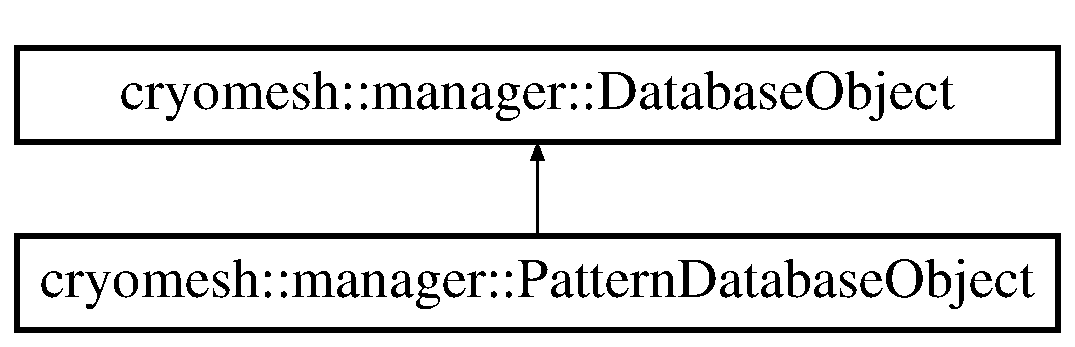
\includegraphics[height=2.000000cm]{classcryomesh_1_1manager_1_1PatternDatabaseObject}
\end{center}
\end{figure}
\subsection*{\-Public \-Member \-Functions}
\begin{DoxyCompactItemize}
\item 
\hyperlink{classcryomesh_1_1manager_1_1PatternDatabaseObject_a880f682507abc648bf30ca5b0572a802}{\-Pattern\-Database\-Object} (const std\-::string uuid\-\_\-str, const \hyperlink{classcryomesh_1_1common_1_1Cycle}{common\-::\-Cycle} \&cyc, const \hyperlink{classcryomesh_1_1state_1_1Pattern}{state\-::\-Pattern} \&pat)
\begin{DoxyCompactList}\small\item\em \-Create database object using pattern and a cycle. \end{DoxyCompactList}\item 
\hyperlink{classcryomesh_1_1manager_1_1PatternDatabaseObject_a77332450f88ed8904d0a0e92527668f3}{\-Pattern\-Database\-Object} (const std\-::string \&node\-\_\-table\-\_\-entry)
\begin{DoxyCompactList}\small\item\em \-Create object from the string of entries in the database output table. \end{DoxyCompactList}\item 
virtual \hyperlink{classcryomesh_1_1manager_1_1PatternDatabaseObject_aa3fc951fe7947592213f569cc375e3e5}{$\sim$\-Pattern\-Database\-Object} ()
\begin{DoxyCompactList}\small\item\em \-Default destructor. \end{DoxyCompactList}\item 
virtual std\-::string \hyperlink{classcryomesh_1_1manager_1_1PatternDatabaseObject_a0f4325cce7fd6c70017815ea50cd4fd6}{get\-Insert} (const std\-::string \&table) const 
\begin{DoxyCompactList}\small\item\em \-Get the string that can be used to insert the sql data. \end{DoxyCompactList}\item 
std\-::string \hyperlink{classcryomesh_1_1manager_1_1PatternDatabaseObject_a28cfc51ab59005adcef9b741f750ae37}{get\-U\-U\-I\-D} () const 
\begin{DoxyCompactList}\small\item\em \-Get uuid variable. \end{DoxyCompactList}\item 
const \hyperlink{classcryomesh_1_1common_1_1Cycle}{common\-::\-Cycle} \& \hyperlink{classcryomesh_1_1manager_1_1PatternDatabaseObject_a7be5ec797560ad735e112fdd0bfa8da2}{get\-Cycle} () const 
\begin{DoxyCompactList}\small\item\em \-Get cycle variable. \end{DoxyCompactList}\item 
const \hyperlink{classcryomesh_1_1state_1_1Pattern}{state\-::\-Pattern} \& \hyperlink{classcryomesh_1_1manager_1_1PatternDatabaseObject_a8d5b7d8bab7eddafe7169ad10842e0ac}{get\-Pattern} () const 
\begin{DoxyCompactList}\small\item\em \-Get pattern variable. \end{DoxyCompactList}\item 
std\-::string \hyperlink{classcryomesh_1_1manager_1_1DatabaseObject_a66ded4e1a1bccd65c94922648c7135c5}{get\-Key} (const std\-::string \&key) const 
\begin{DoxyCompactList}\small\item\em \-Return the string object associated with a key. \end{DoxyCompactList}\end{DoxyCompactItemize}
\subsection*{\-Static \-Public \-Member \-Functions}
\begin{DoxyCompactItemize}
\item 
static std\-::string \hyperlink{classcryomesh_1_1manager_1_1DatabaseObject_aa4ef26ce91fea092f146e67add491e0f}{find\-Value} (const std\-::string \&entry, const std\-::map$<$ std\-::string, std\-::string $>$ \&map)
\begin{DoxyCompactList}\small\item\em \-Find entries value in map or return null. \end{DoxyCompactList}\item 
static std\-::map$<$ std\-::string, \*
std\-::string $>$ \hyperlink{classcryomesh_1_1manager_1_1DatabaseObject_a04ce7c34b51e3290c972121cf2f16565}{get\-Column\-Map\-From\-Entry} (const std\-::string \&entry)
\begin{DoxyCompactList}\small\item\em \-Parse a string database entry, extract columns and values and return a map. \end{DoxyCompactList}\item 
{\footnotesize template$<$class T $>$ }\\static std\-::string \hyperlink{classcryomesh_1_1manager_1_1DatabaseObject_a1b37d9d07009ae1c71f644761d36b468}{to\-String} (\-T obj)
\begin{DoxyCompactList}\small\item\em \-Convert an templated object that can be piped to a stream to a string. \end{DoxyCompactList}\end{DoxyCompactItemize}
\subsection*{\-Static \-Public \-Attributes}
\begin{DoxyCompactItemize}
\item 
static const std\-::string \hyperlink{classcryomesh_1_1manager_1_1PatternDatabaseObject_a3d300a264abb64a0f26e36818df0c228}{\-I\-D\-\_\-\-T\-A\-G} = \char`\"{}id\char`\"{}
\item 
static const std\-::string \hyperlink{classcryomesh_1_1manager_1_1PatternDatabaseObject_ac6763548916adb57eb5b03035049cc12}{\-C\-Y\-C\-L\-E\-\_\-\-T\-A\-G} = \char`\"{}cycle\char`\"{}
\item 
static const std\-::string \hyperlink{classcryomesh_1_1manager_1_1PatternDatabaseObject_ab032a924bb375d4ee41fe8d854d7d9db}{\-P\-A\-T\-T\-E\-R\-N\-\_\-\-T\-A\-G} = \char`\"{}pattern\char`\"{}
\end{DoxyCompactItemize}
\subsection*{\-Protected \-Attributes}
\begin{DoxyCompactItemize}
\item 
std\-::map$<$ std\-::string, \*
std\-::string $>$ \hyperlink{classcryomesh_1_1manager_1_1DatabaseObject_a9c648bf09b9fd8b4d599b0d4f4abf531}{columns}
\end{DoxyCompactItemize}
\subsection*{\-Private \-Attributes}
\begin{DoxyCompactItemize}
\item 
std\-::string \hyperlink{classcryomesh_1_1manager_1_1PatternDatabaseObject_a1bd568034f9f9d08b5ebb7386417f149}{uuid}
\item 
\hyperlink{classcryomesh_1_1common_1_1Cycle}{common\-::\-Cycle} \hyperlink{classcryomesh_1_1manager_1_1PatternDatabaseObject_aadaa9dab4b616e4780b3ca8119ba38b7}{cycle}
\item 
boost\-::shared\-\_\-ptr$<$ \hyperlink{classcryomesh_1_1state_1_1Pattern}{state\-::\-Pattern} $>$ \hyperlink{classcryomesh_1_1manager_1_1PatternDatabaseObject_a473ad5bb9f7b357f39337c1b8712ded6}{pattern}
\end{DoxyCompactItemize}


\subsection{\-Detailed \-Description}


\-Definition at line 22 of file \-Pattern\-Database\-Object.\-h.



\subsection{\-Constructor \& \-Destructor \-Documentation}
\hypertarget{classcryomesh_1_1manager_1_1PatternDatabaseObject_a880f682507abc648bf30ca5b0572a802}{\index{cryomesh\-::manager\-::\-Pattern\-Database\-Object@{cryomesh\-::manager\-::\-Pattern\-Database\-Object}!\-Pattern\-Database\-Object@{\-Pattern\-Database\-Object}}
\index{\-Pattern\-Database\-Object@{\-Pattern\-Database\-Object}!cryomesh::manager::PatternDatabaseObject@{cryomesh\-::manager\-::\-Pattern\-Database\-Object}}
\subsubsection[{\-Pattern\-Database\-Object}]{\setlength{\rightskip}{0pt plus 5cm}{\bf cryomesh\-::manager\-::\-Pattern\-Database\-Object\-::\-Pattern\-Database\-Object} (
\begin{DoxyParamCaption}
\item[{const std\-::string}]{uuid\-\_\-str, }
\item[{const {\bf common\-::\-Cycle} \&}]{cyc, }
\item[{const {\bf state\-::\-Pattern} \&}]{pat}
\end{DoxyParamCaption}
)}}\label{classcryomesh_1_1manager_1_1PatternDatabaseObject_a880f682507abc648bf30ca5b0572a802}


\-Create database object using pattern and a cycle. 



\-Definition at line 19 of file \-Pattern\-Database\-Object.\-cpp.



\-References cryomesh\-::manager\-::\-Database\-Object\-::columns, cycle, \-C\-Y\-C\-L\-E\-\_\-\-T\-A\-G, \-I\-D\-\_\-\-T\-A\-G, pattern, \-P\-A\-T\-T\-E\-R\-N\-\_\-\-T\-A\-G, cryomesh\-::common\-::\-Cycle\-::to\-U\-L\-Int(), and uuid.

\hypertarget{classcryomesh_1_1manager_1_1PatternDatabaseObject_a77332450f88ed8904d0a0e92527668f3}{\index{cryomesh\-::manager\-::\-Pattern\-Database\-Object@{cryomesh\-::manager\-::\-Pattern\-Database\-Object}!\-Pattern\-Database\-Object@{\-Pattern\-Database\-Object}}
\index{\-Pattern\-Database\-Object@{\-Pattern\-Database\-Object}!cryomesh::manager::PatternDatabaseObject@{cryomesh\-::manager\-::\-Pattern\-Database\-Object}}
\subsubsection[{\-Pattern\-Database\-Object}]{\setlength{\rightskip}{0pt plus 5cm}{\bf cryomesh\-::manager\-::\-Pattern\-Database\-Object\-::\-Pattern\-Database\-Object} (
\begin{DoxyParamCaption}
\item[{const std\-::string \&}]{node\-\_\-table\-\_\-entry}
\end{DoxyParamCaption}
)}}\label{classcryomesh_1_1manager_1_1PatternDatabaseObject_a77332450f88ed8904d0a0e92527668f3}


\-Create object from the string of entries in the database output table. 


\begin{DoxyParams}{\-Parameters}
{\em std\-::string} & \-The string of data taken from a output entry in the database node table \\
\hline
\end{DoxyParams}


\-Definition at line 26 of file \-Pattern\-Database\-Object.\-cpp.



\-References cycle, \-C\-Y\-C\-L\-E\-\_\-\-T\-A\-G, cryomesh\-::manager\-::\-Database\-Object\-::find\-Value(), cryomesh\-::manager\-::\-Database\-Object\-::get\-Column\-Map\-From\-Entry(), \-I\-D\-\_\-\-T\-A\-G, pattern, \-P\-A\-T\-T\-E\-R\-N\-\_\-\-T\-A\-G, and uuid.

\hypertarget{classcryomesh_1_1manager_1_1PatternDatabaseObject_aa3fc951fe7947592213f569cc375e3e5}{\index{cryomesh\-::manager\-::\-Pattern\-Database\-Object@{cryomesh\-::manager\-::\-Pattern\-Database\-Object}!$\sim$\-Pattern\-Database\-Object@{$\sim$\-Pattern\-Database\-Object}}
\index{$\sim$\-Pattern\-Database\-Object@{$\sim$\-Pattern\-Database\-Object}!cryomesh::manager::PatternDatabaseObject@{cryomesh\-::manager\-::\-Pattern\-Database\-Object}}
\subsubsection[{$\sim$\-Pattern\-Database\-Object}]{\setlength{\rightskip}{0pt plus 5cm}{\bf cryomesh\-::manager\-::\-Pattern\-Database\-Object\-::$\sim$\-Pattern\-Database\-Object} (
\begin{DoxyParamCaption}
{}
\end{DoxyParamCaption}
)\hspace{0.3cm}{\ttfamily  \mbox{[}virtual\mbox{]}}}}\label{classcryomesh_1_1manager_1_1PatternDatabaseObject_aa3fc951fe7947592213f569cc375e3e5}


\-Default destructor. 



\-Definition at line 38 of file \-Pattern\-Database\-Object.\-cpp.



\subsection{\-Member \-Function \-Documentation}
\hypertarget{classcryomesh_1_1manager_1_1DatabaseObject_aa4ef26ce91fea092f146e67add491e0f}{\index{cryomesh\-::manager\-::\-Pattern\-Database\-Object@{cryomesh\-::manager\-::\-Pattern\-Database\-Object}!find\-Value@{find\-Value}}
\index{find\-Value@{find\-Value}!cryomesh::manager::PatternDatabaseObject@{cryomesh\-::manager\-::\-Pattern\-Database\-Object}}
\subsubsection[{find\-Value}]{\setlength{\rightskip}{0pt plus 5cm}static std\-::string {\bf cryomesh\-::manager\-::\-Database\-Object\-::find\-Value} (
\begin{DoxyParamCaption}
\item[{const std\-::string \&}]{entry, }
\item[{const std\-::map$<$ std\-::string, std\-::string $>$ \&}]{map}
\end{DoxyParamCaption}
)\hspace{0.3cm}{\ttfamily  \mbox{[}inline, static, inherited\mbox{]}}}}\label{classcryomesh_1_1manager_1_1DatabaseObject_aa4ef26ce91fea092f146e67add491e0f}


\-Find entries value in map or return null. 


\begin{DoxyParams}{\-Parameters}
{\em std\-::string} & \-Entry to find \\
\hline
{\em std\-::map$<$std\-::string,std\-::string} & map to search\\
\hline
\end{DoxyParams}
\begin{DoxyReturn}{\-Returns}
\-Value of entry 
\end{DoxyReturn}


\-Definition at line 59 of file \-Database\-Object.\-h.



\-Referenced by cryomesh\-::manager\-::\-Connection\-Database\-Object\-::\-Connection\-Database\-Object(), cryomesh\-::manager\-::\-Node\-Database\-Object\-::\-Node\-Database\-Object(), and \-Pattern\-Database\-Object().

\hypertarget{classcryomesh_1_1manager_1_1DatabaseObject_a04ce7c34b51e3290c972121cf2f16565}{\index{cryomesh\-::manager\-::\-Pattern\-Database\-Object@{cryomesh\-::manager\-::\-Pattern\-Database\-Object}!get\-Column\-Map\-From\-Entry@{get\-Column\-Map\-From\-Entry}}
\index{get\-Column\-Map\-From\-Entry@{get\-Column\-Map\-From\-Entry}!cryomesh::manager::PatternDatabaseObject@{cryomesh\-::manager\-::\-Pattern\-Database\-Object}}
\subsubsection[{get\-Column\-Map\-From\-Entry}]{\setlength{\rightskip}{0pt plus 5cm}static std\-::map$<$std\-::string, std\-::string$>$ {\bf cryomesh\-::manager\-::\-Database\-Object\-::get\-Column\-Map\-From\-Entry} (
\begin{DoxyParamCaption}
\item[{const std\-::string \&}]{entry}
\end{DoxyParamCaption}
)\hspace{0.3cm}{\ttfamily  \mbox{[}inline, static, inherited\mbox{]}}}}\label{classcryomesh_1_1manager_1_1DatabaseObject_a04ce7c34b51e3290c972121cf2f16565}


\-Parse a string database entry, extract columns and values and return a map. 



\-Definition at line 72 of file \-Database\-Object.\-h.



\-Referenced by cryomesh\-::manager\-::\-Connection\-Database\-Object\-::\-Connection\-Database\-Object(), cryomesh\-::manager\-::\-Node\-Database\-Object\-::\-Node\-Database\-Object(), and \-Pattern\-Database\-Object().

\hypertarget{classcryomesh_1_1manager_1_1PatternDatabaseObject_a7be5ec797560ad735e112fdd0bfa8da2}{\index{cryomesh\-::manager\-::\-Pattern\-Database\-Object@{cryomesh\-::manager\-::\-Pattern\-Database\-Object}!get\-Cycle@{get\-Cycle}}
\index{get\-Cycle@{get\-Cycle}!cryomesh::manager::PatternDatabaseObject@{cryomesh\-::manager\-::\-Pattern\-Database\-Object}}
\subsubsection[{get\-Cycle}]{\setlength{\rightskip}{0pt plus 5cm}const {\bf common\-::\-Cycle} \& {\bf cryomesh\-::manager\-::\-Pattern\-Database\-Object\-::get\-Cycle} (
\begin{DoxyParamCaption}
{}
\end{DoxyParamCaption}
) const}}\label{classcryomesh_1_1manager_1_1PatternDatabaseObject_a7be5ec797560ad735e112fdd0bfa8da2}


\-Get cycle variable. 

\begin{DoxyReturn}{\-Returns}
\hyperlink{classcryomesh_1_1common_1_1Cycle}{common\-::\-Cycle} \-The cycle variable 
\end{DoxyReturn}


\-Definition at line 55 of file \-Pattern\-Database\-Object.\-cpp.



\-References cycle.

\hypertarget{classcryomesh_1_1manager_1_1PatternDatabaseObject_a0f4325cce7fd6c70017815ea50cd4fd6}{\index{cryomesh\-::manager\-::\-Pattern\-Database\-Object@{cryomesh\-::manager\-::\-Pattern\-Database\-Object}!get\-Insert@{get\-Insert}}
\index{get\-Insert@{get\-Insert}!cryomesh::manager::PatternDatabaseObject@{cryomesh\-::manager\-::\-Pattern\-Database\-Object}}
\subsubsection[{get\-Insert}]{\setlength{\rightskip}{0pt plus 5cm}std\-::string {\bf cryomesh\-::manager\-::\-Pattern\-Database\-Object\-::get\-Insert} (
\begin{DoxyParamCaption}
\item[{const std\-::string \&}]{table}
\end{DoxyParamCaption}
) const\hspace{0.3cm}{\ttfamily  \mbox{[}virtual\mbox{]}}}}\label{classcryomesh_1_1manager_1_1PatternDatabaseObject_a0f4325cce7fd6c70017815ea50cd4fd6}


\-Get the string that can be used to insert the sql data. 

\begin{DoxyReturn}{\-Returns}
the sql command string to insert into this table 
\end{DoxyReturn}


\-Implements \hyperlink{classcryomesh_1_1manager_1_1DatabaseObject_ad55c6e711341a652790b97f549b0dc63}{cryomesh\-::manager\-::\-Database\-Object}.



\-Definition at line 42 of file \-Pattern\-Database\-Object.\-cpp.



\-References \-C\-Y\-C\-L\-E\-\_\-\-T\-A\-G, cryomesh\-::manager\-::\-Database\-Object\-::get\-Key(), \-I\-D\-\_\-\-T\-A\-G, and \-P\-A\-T\-T\-E\-R\-N\-\_\-\-T\-A\-G.

\hypertarget{classcryomesh_1_1manager_1_1DatabaseObject_a66ded4e1a1bccd65c94922648c7135c5}{\index{cryomesh\-::manager\-::\-Pattern\-Database\-Object@{cryomesh\-::manager\-::\-Pattern\-Database\-Object}!get\-Key@{get\-Key}}
\index{get\-Key@{get\-Key}!cryomesh::manager::PatternDatabaseObject@{cryomesh\-::manager\-::\-Pattern\-Database\-Object}}
\subsubsection[{get\-Key}]{\setlength{\rightskip}{0pt plus 5cm}std\-::string {\bf cryomesh\-::manager\-::\-Database\-Object\-::get\-Key} (
\begin{DoxyParamCaption}
\item[{const std\-::string \&}]{key}
\end{DoxyParamCaption}
) const\hspace{0.3cm}{\ttfamily  \mbox{[}inline, inherited\mbox{]}}}}\label{classcryomesh_1_1manager_1_1DatabaseObject_a66ded4e1a1bccd65c94922648c7135c5}


\-Return the string object associated with a key. 

\-::string \-The key to search for

\begin{DoxyReturn}{\-Returns}
std\-::string \-The object associated with the search key, \char`\"{}\char`\"{} if not found 
\end{DoxyReturn}


\-Definition at line 37 of file \-Database\-Object.\-h.



\-References cryomesh\-::manager\-::\-Database\-Object\-::columns.



\-Referenced by get\-Insert(), cryomesh\-::manager\-::\-Node\-Database\-Object\-::get\-Insert(), and cryomesh\-::manager\-::\-Connection\-Database\-Object\-::get\-Insert().

\hypertarget{classcryomesh_1_1manager_1_1PatternDatabaseObject_a8d5b7d8bab7eddafe7169ad10842e0ac}{\index{cryomesh\-::manager\-::\-Pattern\-Database\-Object@{cryomesh\-::manager\-::\-Pattern\-Database\-Object}!get\-Pattern@{get\-Pattern}}
\index{get\-Pattern@{get\-Pattern}!cryomesh::manager::PatternDatabaseObject@{cryomesh\-::manager\-::\-Pattern\-Database\-Object}}
\subsubsection[{get\-Pattern}]{\setlength{\rightskip}{0pt plus 5cm}const {\bf state\-::\-Pattern} \& {\bf cryomesh\-::manager\-::\-Pattern\-Database\-Object\-::get\-Pattern} (
\begin{DoxyParamCaption}
{}
\end{DoxyParamCaption}
) const}}\label{classcryomesh_1_1manager_1_1PatternDatabaseObject_a8d5b7d8bab7eddafe7169ad10842e0ac}


\-Get pattern variable. 

\begin{DoxyReturn}{\-Returns}
\-Pattern \-The pattern variable 
\end{DoxyReturn}


\-Definition at line 59 of file \-Pattern\-Database\-Object.\-cpp.



\-References pattern.

\hypertarget{classcryomesh_1_1manager_1_1PatternDatabaseObject_a28cfc51ab59005adcef9b741f750ae37}{\index{cryomesh\-::manager\-::\-Pattern\-Database\-Object@{cryomesh\-::manager\-::\-Pattern\-Database\-Object}!get\-U\-U\-I\-D@{get\-U\-U\-I\-D}}
\index{get\-U\-U\-I\-D@{get\-U\-U\-I\-D}!cryomesh::manager::PatternDatabaseObject@{cryomesh\-::manager\-::\-Pattern\-Database\-Object}}
\subsubsection[{get\-U\-U\-I\-D}]{\setlength{\rightskip}{0pt plus 5cm}std\-::string {\bf cryomesh\-::manager\-::\-Pattern\-Database\-Object\-::get\-U\-U\-I\-D} (
\begin{DoxyParamCaption}
{}
\end{DoxyParamCaption}
) const}}\label{classcryomesh_1_1manager_1_1PatternDatabaseObject_a28cfc51ab59005adcef9b741f750ae37}


\-Get uuid variable. 

\begin{DoxyReturn}{\-Returns}
std\-::string \-The uuid variable 
\end{DoxyReturn}


\-Definition at line 52 of file \-Pattern\-Database\-Object.\-cpp.



\-References uuid.

\hypertarget{classcryomesh_1_1manager_1_1DatabaseObject_a1b37d9d07009ae1c71f644761d36b468}{\index{cryomesh\-::manager\-::\-Pattern\-Database\-Object@{cryomesh\-::manager\-::\-Pattern\-Database\-Object}!to\-String@{to\-String}}
\index{to\-String@{to\-String}!cryomesh::manager::PatternDatabaseObject@{cryomesh\-::manager\-::\-Pattern\-Database\-Object}}
\subsubsection[{to\-String}]{\setlength{\rightskip}{0pt plus 5cm}template$<$class T $>$ static std\-::string {\bf cryomesh\-::manager\-::\-Database\-Object\-::to\-String} (
\begin{DoxyParamCaption}
\item[{\-T}]{obj}
\end{DoxyParamCaption}
)\hspace{0.3cm}{\ttfamily  \mbox{[}inline, static, inherited\mbox{]}}}}\label{classcryomesh_1_1manager_1_1DatabaseObject_a1b37d9d07009ae1c71f644761d36b468}


\-Convert an templated object that can be piped to a stream to a string. 


\begin{DoxyParams}{\-Parameters}
{\em \-T} & \-The object to get a string for \\
\hline
\end{DoxyParams}


\-Definition at line 108 of file \-Database\-Object.\-h.



\subsection{\-Member \-Data \-Documentation}
\hypertarget{classcryomesh_1_1manager_1_1DatabaseObject_a9c648bf09b9fd8b4d599b0d4f4abf531}{\index{cryomesh\-::manager\-::\-Pattern\-Database\-Object@{cryomesh\-::manager\-::\-Pattern\-Database\-Object}!columns@{columns}}
\index{columns@{columns}!cryomesh::manager::PatternDatabaseObject@{cryomesh\-::manager\-::\-Pattern\-Database\-Object}}
\subsubsection[{columns}]{\setlength{\rightskip}{0pt plus 5cm}std\-::map$<$std\-::string, std\-::string$>$ {\bf cryomesh\-::manager\-::\-Database\-Object\-::columns}\hspace{0.3cm}{\ttfamily  \mbox{[}protected, inherited\mbox{]}}}}\label{classcryomesh_1_1manager_1_1DatabaseObject_a9c648bf09b9fd8b4d599b0d4f4abf531}


\-Definition at line 119 of file \-Database\-Object.\-h.



\-Referenced by cryomesh\-::manager\-::\-Connection\-Database\-Object\-::\-Connection\-Database\-Object(), cryomesh\-::manager\-::\-Database\-Object\-::get\-Key(), cryomesh\-::manager\-::\-Node\-Database\-Object\-::\-Node\-Database\-Object(), and \-Pattern\-Database\-Object().

\hypertarget{classcryomesh_1_1manager_1_1PatternDatabaseObject_aadaa9dab4b616e4780b3ca8119ba38b7}{\index{cryomesh\-::manager\-::\-Pattern\-Database\-Object@{cryomesh\-::manager\-::\-Pattern\-Database\-Object}!cycle@{cycle}}
\index{cycle@{cycle}!cryomesh::manager::PatternDatabaseObject@{cryomesh\-::manager\-::\-Pattern\-Database\-Object}}
\subsubsection[{cycle}]{\setlength{\rightskip}{0pt plus 5cm}{\bf common\-::\-Cycle} {\bf cryomesh\-::manager\-::\-Pattern\-Database\-Object\-::cycle}\hspace{0.3cm}{\ttfamily  \mbox{[}private\mbox{]}}}}\label{classcryomesh_1_1manager_1_1PatternDatabaseObject_aadaa9dab4b616e4780b3ca8119ba38b7}


\-Definition at line 106 of file \-Pattern\-Database\-Object.\-h.



\-Referenced by get\-Cycle(), and \-Pattern\-Database\-Object().

\hypertarget{classcryomesh_1_1manager_1_1PatternDatabaseObject_ac6763548916adb57eb5b03035049cc12}{\index{cryomesh\-::manager\-::\-Pattern\-Database\-Object@{cryomesh\-::manager\-::\-Pattern\-Database\-Object}!\-C\-Y\-C\-L\-E\-\_\-\-T\-A\-G@{\-C\-Y\-C\-L\-E\-\_\-\-T\-A\-G}}
\index{\-C\-Y\-C\-L\-E\-\_\-\-T\-A\-G@{\-C\-Y\-C\-L\-E\-\_\-\-T\-A\-G}!cryomesh::manager::PatternDatabaseObject@{cryomesh\-::manager\-::\-Pattern\-Database\-Object}}
\subsubsection[{\-C\-Y\-C\-L\-E\-\_\-\-T\-A\-G}]{\setlength{\rightskip}{0pt plus 5cm}const std\-::string {\bf cryomesh\-::manager\-::\-Pattern\-Database\-Object\-::\-C\-Y\-C\-L\-E\-\_\-\-T\-A\-G} = \char`\"{}cycle\char`\"{}\hspace{0.3cm}{\ttfamily  \mbox{[}static\mbox{]}}}}\label{classcryomesh_1_1manager_1_1PatternDatabaseObject_ac6763548916adb57eb5b03035049cc12}


\-Definition at line 85 of file \-Pattern\-Database\-Object.\-h.



\-Referenced by get\-Insert(), and \-Pattern\-Database\-Object().

\hypertarget{classcryomesh_1_1manager_1_1PatternDatabaseObject_a3d300a264abb64a0f26e36818df0c228}{\index{cryomesh\-::manager\-::\-Pattern\-Database\-Object@{cryomesh\-::manager\-::\-Pattern\-Database\-Object}!\-I\-D\-\_\-\-T\-A\-G@{\-I\-D\-\_\-\-T\-A\-G}}
\index{\-I\-D\-\_\-\-T\-A\-G@{\-I\-D\-\_\-\-T\-A\-G}!cryomesh::manager::PatternDatabaseObject@{cryomesh\-::manager\-::\-Pattern\-Database\-Object}}
\subsubsection[{\-I\-D\-\_\-\-T\-A\-G}]{\setlength{\rightskip}{0pt plus 5cm}const std\-::string {\bf cryomesh\-::manager\-::\-Pattern\-Database\-Object\-::\-I\-D\-\_\-\-T\-A\-G} = \char`\"{}id\char`\"{}\hspace{0.3cm}{\ttfamily  \mbox{[}static\mbox{]}}}}\label{classcryomesh_1_1manager_1_1PatternDatabaseObject_a3d300a264abb64a0f26e36818df0c228}


\-Definition at line 79 of file \-Pattern\-Database\-Object.\-h.



\-Referenced by get\-Insert(), and \-Pattern\-Database\-Object().

\hypertarget{classcryomesh_1_1manager_1_1PatternDatabaseObject_a473ad5bb9f7b357f39337c1b8712ded6}{\index{cryomesh\-::manager\-::\-Pattern\-Database\-Object@{cryomesh\-::manager\-::\-Pattern\-Database\-Object}!pattern@{pattern}}
\index{pattern@{pattern}!cryomesh::manager::PatternDatabaseObject@{cryomesh\-::manager\-::\-Pattern\-Database\-Object}}
\subsubsection[{pattern}]{\setlength{\rightskip}{0pt plus 5cm}boost\-::shared\-\_\-ptr$<$ {\bf state\-::\-Pattern} $>$ {\bf cryomesh\-::manager\-::\-Pattern\-Database\-Object\-::pattern}\hspace{0.3cm}{\ttfamily  \mbox{[}private\mbox{]}}}}\label{classcryomesh_1_1manager_1_1PatternDatabaseObject_a473ad5bb9f7b357f39337c1b8712ded6}


\-Definition at line 113 of file \-Pattern\-Database\-Object.\-h.



\-Referenced by get\-Pattern(), and \-Pattern\-Database\-Object().

\hypertarget{classcryomesh_1_1manager_1_1PatternDatabaseObject_ab032a924bb375d4ee41fe8d854d7d9db}{\index{cryomesh\-::manager\-::\-Pattern\-Database\-Object@{cryomesh\-::manager\-::\-Pattern\-Database\-Object}!\-P\-A\-T\-T\-E\-R\-N\-\_\-\-T\-A\-G@{\-P\-A\-T\-T\-E\-R\-N\-\_\-\-T\-A\-G}}
\index{\-P\-A\-T\-T\-E\-R\-N\-\_\-\-T\-A\-G@{\-P\-A\-T\-T\-E\-R\-N\-\_\-\-T\-A\-G}!cryomesh::manager::PatternDatabaseObject@{cryomesh\-::manager\-::\-Pattern\-Database\-Object}}
\subsubsection[{\-P\-A\-T\-T\-E\-R\-N\-\_\-\-T\-A\-G}]{\setlength{\rightskip}{0pt plus 5cm}const std\-::string {\bf cryomesh\-::manager\-::\-Pattern\-Database\-Object\-::\-P\-A\-T\-T\-E\-R\-N\-\_\-\-T\-A\-G} = \char`\"{}pattern\char`\"{}\hspace{0.3cm}{\ttfamily  \mbox{[}static\mbox{]}}}}\label{classcryomesh_1_1manager_1_1PatternDatabaseObject_ab032a924bb375d4ee41fe8d854d7d9db}


\-Definition at line 92 of file \-Pattern\-Database\-Object.\-h.



\-Referenced by get\-Insert(), and \-Pattern\-Database\-Object().

\hypertarget{classcryomesh_1_1manager_1_1PatternDatabaseObject_a1bd568034f9f9d08b5ebb7386417f149}{\index{cryomesh\-::manager\-::\-Pattern\-Database\-Object@{cryomesh\-::manager\-::\-Pattern\-Database\-Object}!uuid@{uuid}}
\index{uuid@{uuid}!cryomesh::manager::PatternDatabaseObject@{cryomesh\-::manager\-::\-Pattern\-Database\-Object}}
\subsubsection[{uuid}]{\setlength{\rightskip}{0pt plus 5cm}std\-::string {\bf cryomesh\-::manager\-::\-Pattern\-Database\-Object\-::uuid}\hspace{0.3cm}{\ttfamily  \mbox{[}private\mbox{]}}}}\label{classcryomesh_1_1manager_1_1PatternDatabaseObject_a1bd568034f9f9d08b5ebb7386417f149}


\-Definition at line 99 of file \-Pattern\-Database\-Object.\-h.



\-Referenced by get\-U\-U\-I\-D(), and \-Pattern\-Database\-Object().



\-The documentation for this class was generated from the following files\-:\begin{DoxyCompactItemize}
\item 
/home/niall/\-Projects/\-Eclipse/\-C\-P\-P/cryomesh/src/manager/\hyperlink{PatternDatabaseObject_8h}{\-Pattern\-Database\-Object.\-h}\item 
/home/niall/\-Projects/\-Eclipse/\-C\-P\-P/cryomesh/src/manager/\hyperlink{PatternDatabaseObject_8cpp}{\-Pattern\-Database\-Object.\-cpp}\end{DoxyCompactItemize}

\hypertarget{classcryomesh_1_1state_1_1PatternTag}{\section{cryomesh\-:\-:state\-:\-:\-Pattern\-Tag \-Class \-Reference}
\label{classcryomesh_1_1state_1_1PatternTag}\index{cryomesh\-::state\-::\-Pattern\-Tag@{cryomesh\-::state\-::\-Pattern\-Tag}}
}


{\ttfamily \#include $<$\-Pattern\-Tag.\-h$>$}

\-Inheritance diagram for cryomesh\-:\-:state\-:\-:\-Pattern\-Tag\-:\begin{figure}[H]
\begin{center}
\leavevmode
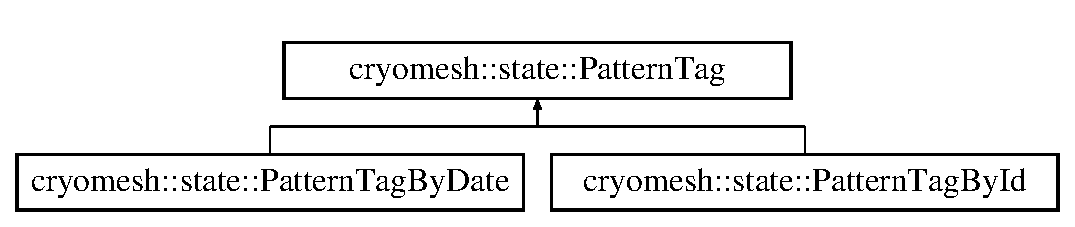
\includegraphics[height=2.000000cm]{classcryomesh_1_1state_1_1PatternTag}
\end{center}
\end{figure}
\subsection*{\-Public \-Member \-Functions}
\begin{DoxyCompactItemize}
\item 
\hyperlink{classcryomesh_1_1state_1_1PatternTag_ab4743b4692605d766378994b87d786ed}{\-Pattern\-Tag} ()
\item 
virtual \hyperlink{classcryomesh_1_1state_1_1PatternTag_aa5239974dfc79638f346145d28ddf961}{$\sim$\-Pattern\-Tag} ()
\item 
virtual std\-::string \hyperlink{classcryomesh_1_1state_1_1PatternTag_a00c56f1f6f348e51a9c02338abf3e5ab}{get\-Tag} () const =0
\item 
virtual void \hyperlink{classcryomesh_1_1state_1_1PatternTag_a17830f089a443437fa736460e231706e}{set\-Tag} (std\-::string tg)=0
\item 
virtual std\-::string \hyperlink{classcryomesh_1_1state_1_1PatternTag_a0b22ab8e03558ed9a2370a66b67761a0}{move\-Tag} ()=0
\item 
virtual std\-::string \hyperlink{classcryomesh_1_1state_1_1PatternTag_ac904d5f971af7e9930ce85a256097c48}{move\-Tag} (int i)=0
\item 
virtual std\-::string \hyperlink{classcryomesh_1_1state_1_1PatternTag_a19284a4419275776a7277af2de158620}{get\-Start\-Tag} () const =0
\item 
virtual std\-::string \hyperlink{classcryomesh_1_1state_1_1PatternTag_ae6a5eb0d13e5152a33de9527c66d358b}{get\-End\-Tag} () const =0
\item 
virtual void \hyperlink{classcryomesh_1_1state_1_1PatternTag_a0c7e050117e2cc5d146b90efad122561}{set\-Start\-Tag} (std\-::string tg)=0
\item 
virtual void \hyperlink{classcryomesh_1_1state_1_1PatternTag_a5026dd228cf678c58267ff343ff84e04}{set\-End\-Tag} (std\-::string tg)=0
\item 
virtual boost\-::shared\-\_\-ptr\*
$<$ \hyperlink{classcryomesh_1_1state_1_1PatternTag}{\-Pattern\-Tag} $>$ \hyperlink{classcryomesh_1_1state_1_1PatternTag_ae689bd0c2045fbb30f482123adfe4657}{get\-Global\-Tag} ()=0
\end{DoxyCompactItemize}


\subsection{\-Detailed \-Description}


\-Definition at line 17 of file \-Pattern\-Tag.\-h.



\subsection{\-Constructor \& \-Destructor \-Documentation}
\hypertarget{classcryomesh_1_1state_1_1PatternTag_ab4743b4692605d766378994b87d786ed}{\index{cryomesh\-::state\-::\-Pattern\-Tag@{cryomesh\-::state\-::\-Pattern\-Tag}!\-Pattern\-Tag@{\-Pattern\-Tag}}
\index{\-Pattern\-Tag@{\-Pattern\-Tag}!cryomesh::state::PatternTag@{cryomesh\-::state\-::\-Pattern\-Tag}}
\subsubsection[{\-Pattern\-Tag}]{\setlength{\rightskip}{0pt plus 5cm}{\bf cryomesh\-::state\-::\-Pattern\-Tag\-::\-Pattern\-Tag} (
\begin{DoxyParamCaption}
{}
\end{DoxyParamCaption}
)\hspace{0.3cm}{\ttfamily  \mbox{[}inline\mbox{]}}}}\label{classcryomesh_1_1state_1_1PatternTag_ab4743b4692605d766378994b87d786ed}


\-Definition at line 19 of file \-Pattern\-Tag.\-h.

\hypertarget{classcryomesh_1_1state_1_1PatternTag_aa5239974dfc79638f346145d28ddf961}{\index{cryomesh\-::state\-::\-Pattern\-Tag@{cryomesh\-::state\-::\-Pattern\-Tag}!$\sim$\-Pattern\-Tag@{$\sim$\-Pattern\-Tag}}
\index{$\sim$\-Pattern\-Tag@{$\sim$\-Pattern\-Tag}!cryomesh::state::PatternTag@{cryomesh\-::state\-::\-Pattern\-Tag}}
\subsubsection[{$\sim$\-Pattern\-Tag}]{\setlength{\rightskip}{0pt plus 5cm}virtual {\bf cryomesh\-::state\-::\-Pattern\-Tag\-::$\sim$\-Pattern\-Tag} (
\begin{DoxyParamCaption}
{}
\end{DoxyParamCaption}
)\hspace{0.3cm}{\ttfamily  \mbox{[}inline, virtual\mbox{]}}}}\label{classcryomesh_1_1state_1_1PatternTag_aa5239974dfc79638f346145d28ddf961}


\-Definition at line 20 of file \-Pattern\-Tag.\-h.



\subsection{\-Member \-Function \-Documentation}
\hypertarget{classcryomesh_1_1state_1_1PatternTag_ae6a5eb0d13e5152a33de9527c66d358b}{\index{cryomesh\-::state\-::\-Pattern\-Tag@{cryomesh\-::state\-::\-Pattern\-Tag}!get\-End\-Tag@{get\-End\-Tag}}
\index{get\-End\-Tag@{get\-End\-Tag}!cryomesh::state::PatternTag@{cryomesh\-::state\-::\-Pattern\-Tag}}
\subsubsection[{get\-End\-Tag}]{\setlength{\rightskip}{0pt plus 5cm}virtual std\-::string {\bf cryomesh\-::state\-::\-Pattern\-Tag\-::get\-End\-Tag} (
\begin{DoxyParamCaption}
{}
\end{DoxyParamCaption}
) const\hspace{0.3cm}{\ttfamily  \mbox{[}pure virtual\mbox{]}}}}\label{classcryomesh_1_1state_1_1PatternTag_ae6a5eb0d13e5152a33de9527c66d358b}


\-Implemented in \hyperlink{classcryomesh_1_1state_1_1PatternTagByDate_a52262ecad476ba4890bd622addd844f2}{cryomesh\-::state\-::\-Pattern\-Tag\-By\-Date}, and \hyperlink{classcryomesh_1_1state_1_1PatternTagById_a9d5f9cc34fd14d895ce235cea35aebe8}{cryomesh\-::state\-::\-Pattern\-Tag\-By\-Id}.

\hypertarget{classcryomesh_1_1state_1_1PatternTag_ae689bd0c2045fbb30f482123adfe4657}{\index{cryomesh\-::state\-::\-Pattern\-Tag@{cryomesh\-::state\-::\-Pattern\-Tag}!get\-Global\-Tag@{get\-Global\-Tag}}
\index{get\-Global\-Tag@{get\-Global\-Tag}!cryomesh::state::PatternTag@{cryomesh\-::state\-::\-Pattern\-Tag}}
\subsubsection[{get\-Global\-Tag}]{\setlength{\rightskip}{0pt plus 5cm}virtual boost\-::shared\-\_\-ptr$<${\bf \-Pattern\-Tag}$>$ {\bf cryomesh\-::state\-::\-Pattern\-Tag\-::get\-Global\-Tag} (
\begin{DoxyParamCaption}
{}
\end{DoxyParamCaption}
)\hspace{0.3cm}{\ttfamily  \mbox{[}pure virtual\mbox{]}}}}\label{classcryomesh_1_1state_1_1PatternTag_ae689bd0c2045fbb30f482123adfe4657}


\-Implemented in \hyperlink{classcryomesh_1_1state_1_1PatternTagByDate_a4a34d0d5566ae8a3888b8c7a747bef6b}{cryomesh\-::state\-::\-Pattern\-Tag\-By\-Date}, and \hyperlink{classcryomesh_1_1state_1_1PatternTagById_ac3dbe345fe252b9ab9feafa995e91474}{cryomesh\-::state\-::\-Pattern\-Tag\-By\-Id}.

\hypertarget{classcryomesh_1_1state_1_1PatternTag_a19284a4419275776a7277af2de158620}{\index{cryomesh\-::state\-::\-Pattern\-Tag@{cryomesh\-::state\-::\-Pattern\-Tag}!get\-Start\-Tag@{get\-Start\-Tag}}
\index{get\-Start\-Tag@{get\-Start\-Tag}!cryomesh::state::PatternTag@{cryomesh\-::state\-::\-Pattern\-Tag}}
\subsubsection[{get\-Start\-Tag}]{\setlength{\rightskip}{0pt plus 5cm}virtual std\-::string {\bf cryomesh\-::state\-::\-Pattern\-Tag\-::get\-Start\-Tag} (
\begin{DoxyParamCaption}
{}
\end{DoxyParamCaption}
) const\hspace{0.3cm}{\ttfamily  \mbox{[}pure virtual\mbox{]}}}}\label{classcryomesh_1_1state_1_1PatternTag_a19284a4419275776a7277af2de158620}


\-Implemented in \hyperlink{classcryomesh_1_1state_1_1PatternTagByDate_aba2a73f929cba2baa5d51965509230e3}{cryomesh\-::state\-::\-Pattern\-Tag\-By\-Date}, and \hyperlink{classcryomesh_1_1state_1_1PatternTagById_ac2624633ba018f4ad1ae229278cfe198}{cryomesh\-::state\-::\-Pattern\-Tag\-By\-Id}.

\hypertarget{classcryomesh_1_1state_1_1PatternTag_a00c56f1f6f348e51a9c02338abf3e5ab}{\index{cryomesh\-::state\-::\-Pattern\-Tag@{cryomesh\-::state\-::\-Pattern\-Tag}!get\-Tag@{get\-Tag}}
\index{get\-Tag@{get\-Tag}!cryomesh::state::PatternTag@{cryomesh\-::state\-::\-Pattern\-Tag}}
\subsubsection[{get\-Tag}]{\setlength{\rightskip}{0pt plus 5cm}virtual std\-::string {\bf cryomesh\-::state\-::\-Pattern\-Tag\-::get\-Tag} (
\begin{DoxyParamCaption}
{}
\end{DoxyParamCaption}
) const\hspace{0.3cm}{\ttfamily  \mbox{[}pure virtual\mbox{]}}}}\label{classcryomesh_1_1state_1_1PatternTag_a00c56f1f6f348e51a9c02338abf3e5ab}


\-Implemented in \hyperlink{classcryomesh_1_1state_1_1PatternTagByDate_a0f01388871f2e3a96d25ab92082cec4b}{cryomesh\-::state\-::\-Pattern\-Tag\-By\-Date}, and \hyperlink{classcryomesh_1_1state_1_1PatternTagById_acee63d4183580398eb30161dfbb3a88d}{cryomesh\-::state\-::\-Pattern\-Tag\-By\-Id}.

\hypertarget{classcryomesh_1_1state_1_1PatternTag_a0b22ab8e03558ed9a2370a66b67761a0}{\index{cryomesh\-::state\-::\-Pattern\-Tag@{cryomesh\-::state\-::\-Pattern\-Tag}!move\-Tag@{move\-Tag}}
\index{move\-Tag@{move\-Tag}!cryomesh::state::PatternTag@{cryomesh\-::state\-::\-Pattern\-Tag}}
\subsubsection[{move\-Tag}]{\setlength{\rightskip}{0pt plus 5cm}virtual std\-::string {\bf cryomesh\-::state\-::\-Pattern\-Tag\-::move\-Tag} (
\begin{DoxyParamCaption}
{}
\end{DoxyParamCaption}
)\hspace{0.3cm}{\ttfamily  \mbox{[}pure virtual\mbox{]}}}}\label{classcryomesh_1_1state_1_1PatternTag_a0b22ab8e03558ed9a2370a66b67761a0}


\-Implemented in \hyperlink{classcryomesh_1_1state_1_1PatternTagByDate_acbd442ea1927dc9eab7683e67d82ab6c}{cryomesh\-::state\-::\-Pattern\-Tag\-By\-Date}, and \hyperlink{classcryomesh_1_1state_1_1PatternTagById_aa8146b29d5b9448d9a73fde4f18c1b70}{cryomesh\-::state\-::\-Pattern\-Tag\-By\-Id}.

\hypertarget{classcryomesh_1_1state_1_1PatternTag_ac904d5f971af7e9930ce85a256097c48}{\index{cryomesh\-::state\-::\-Pattern\-Tag@{cryomesh\-::state\-::\-Pattern\-Tag}!move\-Tag@{move\-Tag}}
\index{move\-Tag@{move\-Tag}!cryomesh::state::PatternTag@{cryomesh\-::state\-::\-Pattern\-Tag}}
\subsubsection[{move\-Tag}]{\setlength{\rightskip}{0pt plus 5cm}virtual std\-::string {\bf cryomesh\-::state\-::\-Pattern\-Tag\-::move\-Tag} (
\begin{DoxyParamCaption}
\item[{int}]{i}
\end{DoxyParamCaption}
)\hspace{0.3cm}{\ttfamily  \mbox{[}pure virtual\mbox{]}}}}\label{classcryomesh_1_1state_1_1PatternTag_ac904d5f971af7e9930ce85a256097c48}


\-Implemented in \hyperlink{classcryomesh_1_1state_1_1PatternTagByDate_aa38857773222e320697dbfede65ed36f}{cryomesh\-::state\-::\-Pattern\-Tag\-By\-Date}, and \hyperlink{classcryomesh_1_1state_1_1PatternTagById_a27fb4f51f07766bd1715b5c8b31454ee}{cryomesh\-::state\-::\-Pattern\-Tag\-By\-Id}.

\hypertarget{classcryomesh_1_1state_1_1PatternTag_a5026dd228cf678c58267ff343ff84e04}{\index{cryomesh\-::state\-::\-Pattern\-Tag@{cryomesh\-::state\-::\-Pattern\-Tag}!set\-End\-Tag@{set\-End\-Tag}}
\index{set\-End\-Tag@{set\-End\-Tag}!cryomesh::state::PatternTag@{cryomesh\-::state\-::\-Pattern\-Tag}}
\subsubsection[{set\-End\-Tag}]{\setlength{\rightskip}{0pt plus 5cm}virtual void {\bf cryomesh\-::state\-::\-Pattern\-Tag\-::set\-End\-Tag} (
\begin{DoxyParamCaption}
\item[{std\-::string}]{tg}
\end{DoxyParamCaption}
)\hspace{0.3cm}{\ttfamily  \mbox{[}pure virtual\mbox{]}}}}\label{classcryomesh_1_1state_1_1PatternTag_a5026dd228cf678c58267ff343ff84e04}


\-Implemented in \hyperlink{classcryomesh_1_1state_1_1PatternTagByDate_a2177a240135e1db32da7c38617a68f31}{cryomesh\-::state\-::\-Pattern\-Tag\-By\-Date}, and \hyperlink{classcryomesh_1_1state_1_1PatternTagById_a02e3ef3349001a9cba60cb5e0fc150cd}{cryomesh\-::state\-::\-Pattern\-Tag\-By\-Id}.

\hypertarget{classcryomesh_1_1state_1_1PatternTag_a0c7e050117e2cc5d146b90efad122561}{\index{cryomesh\-::state\-::\-Pattern\-Tag@{cryomesh\-::state\-::\-Pattern\-Tag}!set\-Start\-Tag@{set\-Start\-Tag}}
\index{set\-Start\-Tag@{set\-Start\-Tag}!cryomesh::state::PatternTag@{cryomesh\-::state\-::\-Pattern\-Tag}}
\subsubsection[{set\-Start\-Tag}]{\setlength{\rightskip}{0pt plus 5cm}virtual void {\bf cryomesh\-::state\-::\-Pattern\-Tag\-::set\-Start\-Tag} (
\begin{DoxyParamCaption}
\item[{std\-::string}]{tg}
\end{DoxyParamCaption}
)\hspace{0.3cm}{\ttfamily  \mbox{[}pure virtual\mbox{]}}}}\label{classcryomesh_1_1state_1_1PatternTag_a0c7e050117e2cc5d146b90efad122561}


\-Implemented in \hyperlink{classcryomesh_1_1state_1_1PatternTagByDate_a9b01bf590164b4644c6d942fc0a3a67b}{cryomesh\-::state\-::\-Pattern\-Tag\-By\-Date}, and \hyperlink{classcryomesh_1_1state_1_1PatternTagById_a9adf0ade652a4e48acd264e11e10e3b7}{cryomesh\-::state\-::\-Pattern\-Tag\-By\-Id}.

\hypertarget{classcryomesh_1_1state_1_1PatternTag_a17830f089a443437fa736460e231706e}{\index{cryomesh\-::state\-::\-Pattern\-Tag@{cryomesh\-::state\-::\-Pattern\-Tag}!set\-Tag@{set\-Tag}}
\index{set\-Tag@{set\-Tag}!cryomesh::state::PatternTag@{cryomesh\-::state\-::\-Pattern\-Tag}}
\subsubsection[{set\-Tag}]{\setlength{\rightskip}{0pt plus 5cm}virtual void {\bf cryomesh\-::state\-::\-Pattern\-Tag\-::set\-Tag} (
\begin{DoxyParamCaption}
\item[{std\-::string}]{tg}
\end{DoxyParamCaption}
)\hspace{0.3cm}{\ttfamily  \mbox{[}pure virtual\mbox{]}}}}\label{classcryomesh_1_1state_1_1PatternTag_a17830f089a443437fa736460e231706e}


\-Implemented in \hyperlink{classcryomesh_1_1state_1_1PatternTagByDate_aae131c046e25f41bcd08b19658ca0cc0}{cryomesh\-::state\-::\-Pattern\-Tag\-By\-Date}, and \hyperlink{classcryomesh_1_1state_1_1PatternTagById_a5cfba8a1a26501eb671f186c0b47ff0c}{cryomesh\-::state\-::\-Pattern\-Tag\-By\-Id}.



\-The documentation for this class was generated from the following file\-:\begin{DoxyCompactItemize}
\item 
/home/niall/\-Projects/\-Eclipse/\-C\-P\-P/cryomesh/src/state/\hyperlink{PatternTag_8h}{\-Pattern\-Tag.\-h}\end{DoxyCompactItemize}

\hypertarget{classcryomesh_1_1state_1_1PatternTagByDate}{\section{cryomesh\-:\-:state\-:\-:\-Pattern\-Tag\-By\-Date \-Class \-Reference}
\label{classcryomesh_1_1state_1_1PatternTagByDate}\index{cryomesh\-::state\-::\-Pattern\-Tag\-By\-Date@{cryomesh\-::state\-::\-Pattern\-Tag\-By\-Date}}
}


{\ttfamily \#include $<$\-Pattern\-Tag\-By\-Date.\-h$>$}

\-Inheritance diagram for cryomesh\-:\-:state\-:\-:\-Pattern\-Tag\-By\-Date\-:\begin{figure}[H]
\begin{center}
\leavevmode
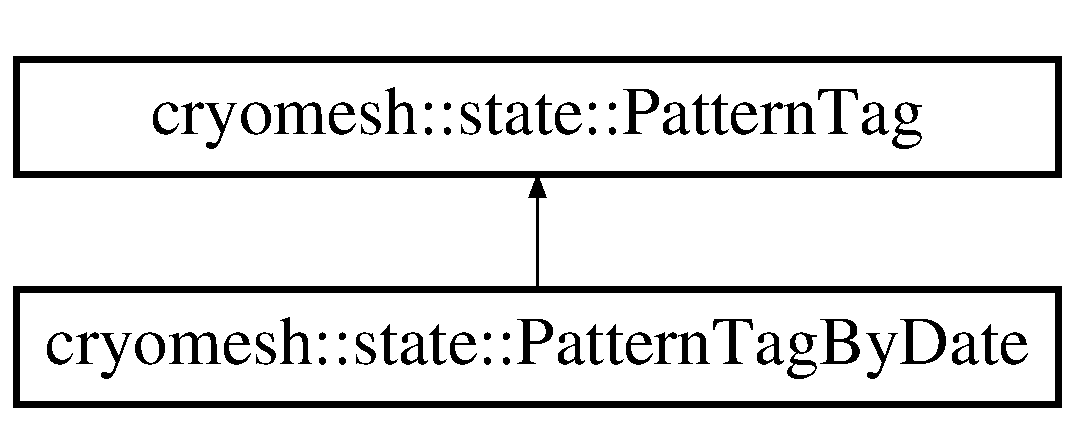
\includegraphics[height=2.000000cm]{classcryomesh_1_1state_1_1PatternTagByDate}
\end{center}
\end{figure}
\subsection*{\-Public \-Types}
\begin{DoxyCompactItemize}
\item 
enum \hyperlink{classcryomesh_1_1state_1_1PatternTagByDate_a0fe44df3214c9397e04ff9a4e8c57ad9}{\-Date\-Type} \{ \*
\hyperlink{classcryomesh_1_1state_1_1PatternTagByDate_a0fe44df3214c9397e04ff9a4e8c57ad9ad826bb03f7153f932902328c419b8f80}{\-By\-Hour}, 
\hyperlink{classcryomesh_1_1state_1_1PatternTagByDate_a0fe44df3214c9397e04ff9a4e8c57ad9aec5bb160aa0c7a042b45a87f0d3f8979}{\-By\-Day}, 
\hyperlink{classcryomesh_1_1state_1_1PatternTagByDate_a0fe44df3214c9397e04ff9a4e8c57ad9a0bd9fc8aa9c2f402cf350ed1043ebbbe}{\-By\-Week}, 
\hyperlink{classcryomesh_1_1state_1_1PatternTagByDate_a0fe44df3214c9397e04ff9a4e8c57ad9ab50088f4741522f6f750fb2b9727e6de}{\-By\-Month}, 
\*
\hyperlink{classcryomesh_1_1state_1_1PatternTagByDate_a0fe44df3214c9397e04ff9a4e8c57ad9a3516aaaf680fa1aaf3eabf97f32fe1a9}{\-By\-Year}
 \}
\end{DoxyCompactItemize}
\subsection*{\-Public \-Member \-Functions}
\begin{DoxyCompactItemize}
\item 
{\footnotesize template$<$class Archive $>$ }\\void \hyperlink{classcryomesh_1_1state_1_1PatternTagByDate_a1b9b91f249940e4f334dcba2e2d783b8}{serialize} (\-Archive \&ar, const unsigned int version)
\item 
\hyperlink{classcryomesh_1_1state_1_1PatternTagByDate_a81779c8abe73f88cf2c165d1a46b34a6}{\-Pattern\-Tag\-By\-Date} (\hyperlink{classcryomesh_1_1state_1_1PatternTagByDate_a0fe44df3214c9397e04ff9a4e8c57ad9}{\-Date\-Type} dt)
\item 
\hyperlink{classcryomesh_1_1state_1_1PatternTagByDate_ad018e686d9f5b6275cd7cc19971a686f}{\-Pattern\-Tag\-By\-Date} (\hyperlink{classcryomesh_1_1state_1_1PatternTagByDate_a0fe44df3214c9397e04ff9a4e8c57ad9}{\-Date\-Type} dt, std\-::tm start\-\_\-time, std\-::tm end\-\_\-time, std\-::tm current\-\_\-time)
\item 
virtual \hyperlink{classcryomesh_1_1state_1_1PatternTagByDate_ac2117051c13a443148321799601d8586}{$\sim$\-Pattern\-Tag\-By\-Date} ()
\item 
virtual std\-::string \hyperlink{classcryomesh_1_1state_1_1PatternTagByDate_a0f01388871f2e3a96d25ab92082cec4b}{get\-Tag} () const 
\item 
virtual void \hyperlink{classcryomesh_1_1state_1_1PatternTagByDate_aae131c046e25f41bcd08b19658ca0cc0}{set\-Tag} (std\-::string tg)
\item 
virtual std\-::string \hyperlink{classcryomesh_1_1state_1_1PatternTagByDate_acbd442ea1927dc9eab7683e67d82ab6c}{move\-Tag} ()
\item 
virtual std\-::string \hyperlink{classcryomesh_1_1state_1_1PatternTagByDate_aa38857773222e320697dbfede65ed36f}{move\-Tag} (int i)
\item 
virtual std\-::string \hyperlink{classcryomesh_1_1state_1_1PatternTagByDate_aba2a73f929cba2baa5d51965509230e3}{get\-Start\-Tag} () const 
\item 
virtual void \hyperlink{classcryomesh_1_1state_1_1PatternTagByDate_a9b01bf590164b4644c6d942fc0a3a67b}{set\-Start\-Tag} (std\-::string tg)
\item 
virtual std\-::string \hyperlink{classcryomesh_1_1state_1_1PatternTagByDate_a52262ecad476ba4890bd622addd844f2}{get\-End\-Tag} () const 
\item 
virtual void \hyperlink{classcryomesh_1_1state_1_1PatternTagByDate_a2177a240135e1db32da7c38617a68f31}{set\-End\-Tag} (std\-::string tg)
\item 
virtual boost\-::shared\-\_\-ptr\*
$<$ \hyperlink{classcryomesh_1_1state_1_1PatternTag}{\-Pattern\-Tag} $>$ \hyperlink{classcryomesh_1_1state_1_1PatternTagByDate_a4a34d0d5566ae8a3888b8c7a747bef6b}{get\-Global\-Tag} ()
\end{DoxyCompactItemize}
\subsection*{\-Static \-Public \-Member \-Functions}
\begin{DoxyCompactItemize}
\item 
static std\-::tm \hyperlink{classcryomesh_1_1state_1_1PatternTagByDate_a783b2953283a8478f6919fd304cb69f1}{tag\-To\-Tm} (const std\-::string \&tg)
\item 
static std\-::string \hyperlink{classcryomesh_1_1state_1_1PatternTagByDate_a8c7d0a7aa8bf92aa05c2ea8ae2c60700}{tm\-To\-Tag} (const std\-::tm \&t)
\item 
static std\-::tm \hyperlink{classcryomesh_1_1state_1_1PatternTagByDate_ae0e700b6ce6d8b84e97e8b3e551fde57}{move\-Hour} (std\-::tm \&ttime, int i)
\item 
static std\-::tm \hyperlink{classcryomesh_1_1state_1_1PatternTagByDate_a9911819de318f1d49f04c67110dd95cd}{move\-Day} (std\-::tm \&ttime, int i)
\item 
static std\-::tm \hyperlink{classcryomesh_1_1state_1_1PatternTagByDate_a589ad778ee7350673d25c553bda0eb83}{move\-Week} (std\-::tm \&ttime, int i)
\item 
static std\-::tm \hyperlink{classcryomesh_1_1state_1_1PatternTagByDate_a04a41144a760e5a85c0aa4d7b05fdb30}{move\-Month} (std\-::tm \&ttime, int i)
\item 
static std\-::tm \hyperlink{classcryomesh_1_1state_1_1PatternTagByDate_ab47ab805764e76faff1791594fa83770}{move\-Year} (std\-::tm \&ttime, int i)
\item 
static bool \hyperlink{classcryomesh_1_1state_1_1PatternTagByDate_a20516b67d8c03a508c0b30395fd2784a}{is\-Leap\-Year} (const std\-::tm \&tmtime)
\end{DoxyCompactItemize}
\subsection*{\-Static \-Protected \-Attributes}
\begin{DoxyCompactItemize}
\item 
static std\-::string \hyperlink{classcryomesh_1_1state_1_1PatternTagByDate_add7aad1fe2fa9ba68a1f6efba392164b}{\-Global\-Start\-Tag} = \char`\"{}\char`\"{}
\item 
static std\-::string \hyperlink{classcryomesh_1_1state_1_1PatternTagByDate_a3e16a76aea6ea2d84e8f90fb9a861a3d}{\-Global\-End\-Tag} = \char`\"{}\char`\"{}
\item 
static std\-::string \hyperlink{classcryomesh_1_1state_1_1PatternTagByDate_a9fd6ba74e86f3f438e9853bd342a0842}{\-Global\-Current\-Tag} = \char`\"{}\char`\"{}
\item 
static std\-::string \hyperlink{classcryomesh_1_1state_1_1PatternTagByDate_aa377c0641330487a3249f710b92ae7b1}{\-Date\-Format} = \char`\"{}\%\-S \%\-M \%\-H \%d \%m \%\-Y \%w \%j \char`\"{}
\end{DoxyCompactItemize}
\subsection*{\-Private \-Attributes}
\begin{DoxyCompactItemize}
\item 
\hyperlink{classcryomesh_1_1state_1_1PatternTagByDate_a0fe44df3214c9397e04ff9a4e8c57ad9}{\-Date\-Type} \hyperlink{classcryomesh_1_1state_1_1PatternTagByDate_a978cee17d8215fcf90a050a033cab7ec}{date\-Type}
\item 
std\-::tm \hyperlink{classcryomesh_1_1state_1_1PatternTagByDate_afe5398940c00ed0fd3b70dcb52efea1c}{start\-Time}
\item 
std\-::tm \hyperlink{classcryomesh_1_1state_1_1PatternTagByDate_a7d1640030846523333a228078cd72acc}{end\-Time}
\item 
std\-::tm \hyperlink{classcryomesh_1_1state_1_1PatternTagByDate_ad80a0a36ec25f13a65c8beadc349c58c}{current\-Time}
\end{DoxyCompactItemize}
\subsection*{\-Static \-Private \-Attributes}
\begin{DoxyCompactItemize}
\item 
static boost\-::shared\-\_\-ptr\*
$<$ \hyperlink{classcryomesh_1_1state_1_1PatternTagByDate}{\-Pattern\-Tag\-By\-Date} $>$ \hyperlink{classcryomesh_1_1state_1_1PatternTagByDate_ac1d93cdd406b287fd3a008102e1d046c}{global\-Tag}
\end{DoxyCompactItemize}
\subsection*{\-Friends}
\begin{DoxyCompactItemize}
\item 
class \hyperlink{classcryomesh_1_1state_1_1PatternTagByDate_ac98d07dd8f7b70e16ccb9a01abf56b9c}{boost\-::serialization\-::access}
\end{DoxyCompactItemize}


\subsection{\-Detailed \-Description}


\-Definition at line 20 of file \-Pattern\-Tag\-By\-Date.\-h.



\subsection{\-Member \-Enumeration \-Documentation}
\hypertarget{classcryomesh_1_1state_1_1PatternTagByDate_a0fe44df3214c9397e04ff9a4e8c57ad9}{\index{cryomesh\-::state\-::\-Pattern\-Tag\-By\-Date@{cryomesh\-::state\-::\-Pattern\-Tag\-By\-Date}!\-Date\-Type@{\-Date\-Type}}
\index{\-Date\-Type@{\-Date\-Type}!cryomesh::state::PatternTagByDate@{cryomesh\-::state\-::\-Pattern\-Tag\-By\-Date}}
\subsubsection[{\-Date\-Type}]{\setlength{\rightskip}{0pt plus 5cm}enum {\bf cryomesh\-::state\-::\-Pattern\-Tag\-By\-Date\-::\-Date\-Type}}}\label{classcryomesh_1_1state_1_1PatternTagByDate_a0fe44df3214c9397e04ff9a4e8c57ad9}
\begin{Desc}
\item[\-Enumerator\-: ]\par
\begin{description}
\index{\-By\-Hour@{\-By\-Hour}!cryomesh\-::state\-::\-Pattern\-Tag\-By\-Date@{cryomesh\-::state\-::\-Pattern\-Tag\-By\-Date}}\index{cryomesh\-::state\-::\-Pattern\-Tag\-By\-Date@{cryomesh\-::state\-::\-Pattern\-Tag\-By\-Date}!\-By\-Hour@{\-By\-Hour}}\item[{\em 
\hypertarget{classcryomesh_1_1state_1_1PatternTagByDate_a0fe44df3214c9397e04ff9a4e8c57ad9ad826bb03f7153f932902328c419b8f80}{\-By\-Hour}\label{classcryomesh_1_1state_1_1PatternTagByDate_a0fe44df3214c9397e04ff9a4e8c57ad9ad826bb03f7153f932902328c419b8f80}
}]\index{\-By\-Day@{\-By\-Day}!cryomesh\-::state\-::\-Pattern\-Tag\-By\-Date@{cryomesh\-::state\-::\-Pattern\-Tag\-By\-Date}}\index{cryomesh\-::state\-::\-Pattern\-Tag\-By\-Date@{cryomesh\-::state\-::\-Pattern\-Tag\-By\-Date}!\-By\-Day@{\-By\-Day}}\item[{\em 
\hypertarget{classcryomesh_1_1state_1_1PatternTagByDate_a0fe44df3214c9397e04ff9a4e8c57ad9aec5bb160aa0c7a042b45a87f0d3f8979}{\-By\-Day}\label{classcryomesh_1_1state_1_1PatternTagByDate_a0fe44df3214c9397e04ff9a4e8c57ad9aec5bb160aa0c7a042b45a87f0d3f8979}
}]\index{\-By\-Week@{\-By\-Week}!cryomesh\-::state\-::\-Pattern\-Tag\-By\-Date@{cryomesh\-::state\-::\-Pattern\-Tag\-By\-Date}}\index{cryomesh\-::state\-::\-Pattern\-Tag\-By\-Date@{cryomesh\-::state\-::\-Pattern\-Tag\-By\-Date}!\-By\-Week@{\-By\-Week}}\item[{\em 
\hypertarget{classcryomesh_1_1state_1_1PatternTagByDate_a0fe44df3214c9397e04ff9a4e8c57ad9a0bd9fc8aa9c2f402cf350ed1043ebbbe}{\-By\-Week}\label{classcryomesh_1_1state_1_1PatternTagByDate_a0fe44df3214c9397e04ff9a4e8c57ad9a0bd9fc8aa9c2f402cf350ed1043ebbbe}
}]\index{\-By\-Month@{\-By\-Month}!cryomesh\-::state\-::\-Pattern\-Tag\-By\-Date@{cryomesh\-::state\-::\-Pattern\-Tag\-By\-Date}}\index{cryomesh\-::state\-::\-Pattern\-Tag\-By\-Date@{cryomesh\-::state\-::\-Pattern\-Tag\-By\-Date}!\-By\-Month@{\-By\-Month}}\item[{\em 
\hypertarget{classcryomesh_1_1state_1_1PatternTagByDate_a0fe44df3214c9397e04ff9a4e8c57ad9ab50088f4741522f6f750fb2b9727e6de}{\-By\-Month}\label{classcryomesh_1_1state_1_1PatternTagByDate_a0fe44df3214c9397e04ff9a4e8c57ad9ab50088f4741522f6f750fb2b9727e6de}
}]\index{\-By\-Year@{\-By\-Year}!cryomesh\-::state\-::\-Pattern\-Tag\-By\-Date@{cryomesh\-::state\-::\-Pattern\-Tag\-By\-Date}}\index{cryomesh\-::state\-::\-Pattern\-Tag\-By\-Date@{cryomesh\-::state\-::\-Pattern\-Tag\-By\-Date}!\-By\-Year@{\-By\-Year}}\item[{\em 
\hypertarget{classcryomesh_1_1state_1_1PatternTagByDate_a0fe44df3214c9397e04ff9a4e8c57ad9a3516aaaf680fa1aaf3eabf97f32fe1a9}{\-By\-Year}\label{classcryomesh_1_1state_1_1PatternTagByDate_a0fe44df3214c9397e04ff9a4e8c57ad9a3516aaaf680fa1aaf3eabf97f32fe1a9}
}]\end{description}
\end{Desc}



\-Definition at line 22 of file \-Pattern\-Tag\-By\-Date.\-h.



\subsection{\-Constructor \& \-Destructor \-Documentation}
\hypertarget{classcryomesh_1_1state_1_1PatternTagByDate_a81779c8abe73f88cf2c165d1a46b34a6}{\index{cryomesh\-::state\-::\-Pattern\-Tag\-By\-Date@{cryomesh\-::state\-::\-Pattern\-Tag\-By\-Date}!\-Pattern\-Tag\-By\-Date@{\-Pattern\-Tag\-By\-Date}}
\index{\-Pattern\-Tag\-By\-Date@{\-Pattern\-Tag\-By\-Date}!cryomesh::state::PatternTagByDate@{cryomesh\-::state\-::\-Pattern\-Tag\-By\-Date}}
\subsubsection[{\-Pattern\-Tag\-By\-Date}]{\setlength{\rightskip}{0pt plus 5cm}{\bf cryomesh\-::state\-::\-Pattern\-Tag\-By\-Date\-::\-Pattern\-Tag\-By\-Date} (
\begin{DoxyParamCaption}
\item[{{\bf \-Date\-Type}}]{dt}
\end{DoxyParamCaption}
)}}\label{classcryomesh_1_1state_1_1PatternTagByDate_a81779c8abe73f88cf2c165d1a46b34a6}


\-Definition at line 22 of file \-Pattern\-Tag\-By\-Date.\-cpp.

\hypertarget{classcryomesh_1_1state_1_1PatternTagByDate_ad018e686d9f5b6275cd7cc19971a686f}{\index{cryomesh\-::state\-::\-Pattern\-Tag\-By\-Date@{cryomesh\-::state\-::\-Pattern\-Tag\-By\-Date}!\-Pattern\-Tag\-By\-Date@{\-Pattern\-Tag\-By\-Date}}
\index{\-Pattern\-Tag\-By\-Date@{\-Pattern\-Tag\-By\-Date}!cryomesh::state::PatternTagByDate@{cryomesh\-::state\-::\-Pattern\-Tag\-By\-Date}}
\subsubsection[{\-Pattern\-Tag\-By\-Date}]{\setlength{\rightskip}{0pt plus 5cm}{\bf cryomesh\-::state\-::\-Pattern\-Tag\-By\-Date\-::\-Pattern\-Tag\-By\-Date} (
\begin{DoxyParamCaption}
\item[{{\bf \-Date\-Type}}]{dt, }
\item[{std\-::tm}]{start\-\_\-time, }
\item[{std\-::tm}]{end\-\_\-time, }
\item[{std\-::tm}]{current\-\_\-time}
\end{DoxyParamCaption}
)}}\label{classcryomesh_1_1state_1_1PatternTagByDate_ad018e686d9f5b6275cd7cc19971a686f}


\-Definition at line 26 of file \-Pattern\-Tag\-By\-Date.\-cpp.



\-References \-Global\-End\-Tag, \-Global\-Start\-Tag, global\-Tag, and start\-Time.

\hypertarget{classcryomesh_1_1state_1_1PatternTagByDate_ac2117051c13a443148321799601d8586}{\index{cryomesh\-::state\-::\-Pattern\-Tag\-By\-Date@{cryomesh\-::state\-::\-Pattern\-Tag\-By\-Date}!$\sim$\-Pattern\-Tag\-By\-Date@{$\sim$\-Pattern\-Tag\-By\-Date}}
\index{$\sim$\-Pattern\-Tag\-By\-Date@{$\sim$\-Pattern\-Tag\-By\-Date}!cryomesh::state::PatternTagByDate@{cryomesh\-::state\-::\-Pattern\-Tag\-By\-Date}}
\subsubsection[{$\sim$\-Pattern\-Tag\-By\-Date}]{\setlength{\rightskip}{0pt plus 5cm}{\bf cryomesh\-::state\-::\-Pattern\-Tag\-By\-Date\-::$\sim$\-Pattern\-Tag\-By\-Date} (
\begin{DoxyParamCaption}
{}
\end{DoxyParamCaption}
)\hspace{0.3cm}{\ttfamily  \mbox{[}virtual\mbox{]}}}}\label{classcryomesh_1_1state_1_1PatternTagByDate_ac2117051c13a443148321799601d8586}


\-Definition at line 34 of file \-Pattern\-Tag\-By\-Date.\-cpp.



\subsection{\-Member \-Function \-Documentation}
\hypertarget{classcryomesh_1_1state_1_1PatternTagByDate_a52262ecad476ba4890bd622addd844f2}{\index{cryomesh\-::state\-::\-Pattern\-Tag\-By\-Date@{cryomesh\-::state\-::\-Pattern\-Tag\-By\-Date}!get\-End\-Tag@{get\-End\-Tag}}
\index{get\-End\-Tag@{get\-End\-Tag}!cryomesh::state::PatternTagByDate@{cryomesh\-::state\-::\-Pattern\-Tag\-By\-Date}}
\subsubsection[{get\-End\-Tag}]{\setlength{\rightskip}{0pt plus 5cm}std\-::string {\bf cryomesh\-::state\-::\-Pattern\-Tag\-By\-Date\-::get\-End\-Tag} (
\begin{DoxyParamCaption}
{}
\end{DoxyParamCaption}
) const\hspace{0.3cm}{\ttfamily  \mbox{[}virtual\mbox{]}}}}\label{classcryomesh_1_1state_1_1PatternTagByDate_a52262ecad476ba4890bd622addd844f2}


\-Implements \hyperlink{classcryomesh_1_1state_1_1PatternTag_ae6a5eb0d13e5152a33de9527c66d358b}{cryomesh\-::state\-::\-Pattern\-Tag}.



\-Definition at line 70 of file \-Pattern\-Tag\-By\-Date.\-cpp.



\-References end\-Time, and tm\-To\-Tag().

\hypertarget{classcryomesh_1_1state_1_1PatternTagByDate_a4a34d0d5566ae8a3888b8c7a747bef6b}{\index{cryomesh\-::state\-::\-Pattern\-Tag\-By\-Date@{cryomesh\-::state\-::\-Pattern\-Tag\-By\-Date}!get\-Global\-Tag@{get\-Global\-Tag}}
\index{get\-Global\-Tag@{get\-Global\-Tag}!cryomesh::state::PatternTagByDate@{cryomesh\-::state\-::\-Pattern\-Tag\-By\-Date}}
\subsubsection[{get\-Global\-Tag}]{\setlength{\rightskip}{0pt plus 5cm}boost\-::shared\-\_\-ptr$<$ {\bf \-Pattern\-Tag} $>$ {\bf cryomesh\-::state\-::\-Pattern\-Tag\-By\-Date\-::get\-Global\-Tag} (
\begin{DoxyParamCaption}
{}
\end{DoxyParamCaption}
)\hspace{0.3cm}{\ttfamily  \mbox{[}virtual\mbox{]}}}}\label{classcryomesh_1_1state_1_1PatternTagByDate_a4a34d0d5566ae8a3888b8c7a747bef6b}


\-Implements \hyperlink{classcryomesh_1_1state_1_1PatternTag_ae689bd0c2045fbb30f482123adfe4657}{cryomesh\-::state\-::\-Pattern\-Tag}.



\-Definition at line 77 of file \-Pattern\-Tag\-By\-Date.\-cpp.



\-References global\-Tag.

\hypertarget{classcryomesh_1_1state_1_1PatternTagByDate_aba2a73f929cba2baa5d51965509230e3}{\index{cryomesh\-::state\-::\-Pattern\-Tag\-By\-Date@{cryomesh\-::state\-::\-Pattern\-Tag\-By\-Date}!get\-Start\-Tag@{get\-Start\-Tag}}
\index{get\-Start\-Tag@{get\-Start\-Tag}!cryomesh::state::PatternTagByDate@{cryomesh\-::state\-::\-Pattern\-Tag\-By\-Date}}
\subsubsection[{get\-Start\-Tag}]{\setlength{\rightskip}{0pt plus 5cm}std\-::string {\bf cryomesh\-::state\-::\-Pattern\-Tag\-By\-Date\-::get\-Start\-Tag} (
\begin{DoxyParamCaption}
{}
\end{DoxyParamCaption}
) const\hspace{0.3cm}{\ttfamily  \mbox{[}virtual\mbox{]}}}}\label{classcryomesh_1_1state_1_1PatternTagByDate_aba2a73f929cba2baa5d51965509230e3}


\-Implements \hyperlink{classcryomesh_1_1state_1_1PatternTag_a19284a4419275776a7277af2de158620}{cryomesh\-::state\-::\-Pattern\-Tag}.



\-Definition at line 64 of file \-Pattern\-Tag\-By\-Date.\-cpp.



\-References start\-Time, and tm\-To\-Tag().

\hypertarget{classcryomesh_1_1state_1_1PatternTagByDate_a0f01388871f2e3a96d25ab92082cec4b}{\index{cryomesh\-::state\-::\-Pattern\-Tag\-By\-Date@{cryomesh\-::state\-::\-Pattern\-Tag\-By\-Date}!get\-Tag@{get\-Tag}}
\index{get\-Tag@{get\-Tag}!cryomesh::state::PatternTagByDate@{cryomesh\-::state\-::\-Pattern\-Tag\-By\-Date}}
\subsubsection[{get\-Tag}]{\setlength{\rightskip}{0pt plus 5cm}std\-::string {\bf cryomesh\-::state\-::\-Pattern\-Tag\-By\-Date\-::get\-Tag} (
\begin{DoxyParamCaption}
{}
\end{DoxyParamCaption}
) const\hspace{0.3cm}{\ttfamily  \mbox{[}virtual\mbox{]}}}}\label{classcryomesh_1_1state_1_1PatternTagByDate_a0f01388871f2e3a96d25ab92082cec4b}


\-Implements \hyperlink{classcryomesh_1_1state_1_1PatternTag_a00c56f1f6f348e51a9c02338abf3e5ab}{cryomesh\-::state\-::\-Pattern\-Tag}.



\-Definition at line 37 of file \-Pattern\-Tag\-By\-Date.\-cpp.



\-References current\-Time, and tm\-To\-Tag().

\hypertarget{classcryomesh_1_1state_1_1PatternTagByDate_a20516b67d8c03a508c0b30395fd2784a}{\index{cryomesh\-::state\-::\-Pattern\-Tag\-By\-Date@{cryomesh\-::state\-::\-Pattern\-Tag\-By\-Date}!is\-Leap\-Year@{is\-Leap\-Year}}
\index{is\-Leap\-Year@{is\-Leap\-Year}!cryomesh::state::PatternTagByDate@{cryomesh\-::state\-::\-Pattern\-Tag\-By\-Date}}
\subsubsection[{is\-Leap\-Year}]{\setlength{\rightskip}{0pt plus 5cm}bool {\bf cryomesh\-::state\-::\-Pattern\-Tag\-By\-Date\-::is\-Leap\-Year} (
\begin{DoxyParamCaption}
\item[{const std\-::tm \&}]{tmtime}
\end{DoxyParamCaption}
)\hspace{0.3cm}{\ttfamily  \mbox{[}static\mbox{]}}}}\label{classcryomesh_1_1state_1_1PatternTagByDate_a20516b67d8c03a508c0b30395fd2784a}


\-Definition at line 206 of file \-Pattern\-Tag\-By\-Date.\-cpp.



\-Referenced by move\-Month(), and move\-Year().

\hypertarget{classcryomesh_1_1state_1_1PatternTagByDate_a9911819de318f1d49f04c67110dd95cd}{\index{cryomesh\-::state\-::\-Pattern\-Tag\-By\-Date@{cryomesh\-::state\-::\-Pattern\-Tag\-By\-Date}!move\-Day@{move\-Day}}
\index{move\-Day@{move\-Day}!cryomesh::state::PatternTagByDate@{cryomesh\-::state\-::\-Pattern\-Tag\-By\-Date}}
\subsubsection[{move\-Day}]{\setlength{\rightskip}{0pt plus 5cm}std\-::tm {\bf cryomesh\-::state\-::\-Pattern\-Tag\-By\-Date\-::move\-Day} (
\begin{DoxyParamCaption}
\item[{std\-::tm \&}]{ttime, }
\item[{int}]{i}
\end{DoxyParamCaption}
)\hspace{0.3cm}{\ttfamily  \mbox{[}static\mbox{]}}}}\label{classcryomesh_1_1state_1_1PatternTagByDate_a9911819de318f1d49f04c67110dd95cd}


\-Definition at line 151 of file \-Pattern\-Tag\-By\-Date.\-cpp.



\-References move\-Hour().



\-Referenced by move\-Month(), move\-Tag(), move\-Week(), and move\-Year().

\hypertarget{classcryomesh_1_1state_1_1PatternTagByDate_ae0e700b6ce6d8b84e97e8b3e551fde57}{\index{cryomesh\-::state\-::\-Pattern\-Tag\-By\-Date@{cryomesh\-::state\-::\-Pattern\-Tag\-By\-Date}!move\-Hour@{move\-Hour}}
\index{move\-Hour@{move\-Hour}!cryomesh::state::PatternTagByDate@{cryomesh\-::state\-::\-Pattern\-Tag\-By\-Date}}
\subsubsection[{move\-Hour}]{\setlength{\rightskip}{0pt plus 5cm}std\-::tm {\bf cryomesh\-::state\-::\-Pattern\-Tag\-By\-Date\-::move\-Hour} (
\begin{DoxyParamCaption}
\item[{std\-::tm \&}]{ttime, }
\item[{int}]{i}
\end{DoxyParamCaption}
)\hspace{0.3cm}{\ttfamily  \mbox{[}static\mbox{]}}}}\label{classcryomesh_1_1state_1_1PatternTagByDate_ae0e700b6ce6d8b84e97e8b3e551fde57}


\-Definition at line 139 of file \-Pattern\-Tag\-By\-Date.\-cpp.



\-Referenced by move\-Day(), and move\-Tag().

\hypertarget{classcryomesh_1_1state_1_1PatternTagByDate_a04a41144a760e5a85c0aa4d7b05fdb30}{\index{cryomesh\-::state\-::\-Pattern\-Tag\-By\-Date@{cryomesh\-::state\-::\-Pattern\-Tag\-By\-Date}!move\-Month@{move\-Month}}
\index{move\-Month@{move\-Month}!cryomesh::state::PatternTagByDate@{cryomesh\-::state\-::\-Pattern\-Tag\-By\-Date}}
\subsubsection[{move\-Month}]{\setlength{\rightskip}{0pt plus 5cm}std\-::tm {\bf cryomesh\-::state\-::\-Pattern\-Tag\-By\-Date\-::move\-Month} (
\begin{DoxyParamCaption}
\item[{std\-::tm \&}]{ttime, }
\item[{int}]{i}
\end{DoxyParamCaption}
)\hspace{0.3cm}{\ttfamily  \mbox{[}static\mbox{]}}}}\label{classcryomesh_1_1state_1_1PatternTagByDate_a04a41144a760e5a85c0aa4d7b05fdb30}


\-Definition at line 161 of file \-Pattern\-Tag\-By\-Date.\-cpp.



\-References is\-Leap\-Year(), move\-Day(), and move\-Year().



\-Referenced by move\-Tag().

\hypertarget{classcryomesh_1_1state_1_1PatternTagByDate_acbd442ea1927dc9eab7683e67d82ab6c}{\index{cryomesh\-::state\-::\-Pattern\-Tag\-By\-Date@{cryomesh\-::state\-::\-Pattern\-Tag\-By\-Date}!move\-Tag@{move\-Tag}}
\index{move\-Tag@{move\-Tag}!cryomesh::state::PatternTagByDate@{cryomesh\-::state\-::\-Pattern\-Tag\-By\-Date}}
\subsubsection[{move\-Tag}]{\setlength{\rightskip}{0pt plus 5cm}std\-::string {\bf cryomesh\-::state\-::\-Pattern\-Tag\-By\-Date\-::move\-Tag} (
\begin{DoxyParamCaption}
{}
\end{DoxyParamCaption}
)\hspace{0.3cm}{\ttfamily  \mbox{[}virtual\mbox{]}}}}\label{classcryomesh_1_1state_1_1PatternTagByDate_acbd442ea1927dc9eab7683e67d82ab6c}


\-Implements \hyperlink{classcryomesh_1_1state_1_1PatternTag_a0b22ab8e03558ed9a2370a66b67761a0}{cryomesh\-::state\-::\-Pattern\-Tag}.



\-Definition at line 43 of file \-Pattern\-Tag\-By\-Date.\-cpp.



\-References \-By\-Day, \-By\-Hour, \-By\-Month, \-By\-Week, \-By\-Year, current\-Time, date\-Type, move\-Day(), move\-Hour(), move\-Month(), move\-Week(), move\-Year(), and tm\-To\-Tag().



\-Referenced by move\-Tag().

\hypertarget{classcryomesh_1_1state_1_1PatternTagByDate_aa38857773222e320697dbfede65ed36f}{\index{cryomesh\-::state\-::\-Pattern\-Tag\-By\-Date@{cryomesh\-::state\-::\-Pattern\-Tag\-By\-Date}!move\-Tag@{move\-Tag}}
\index{move\-Tag@{move\-Tag}!cryomesh::state::PatternTagByDate@{cryomesh\-::state\-::\-Pattern\-Tag\-By\-Date}}
\subsubsection[{move\-Tag}]{\setlength{\rightskip}{0pt plus 5cm}std\-::string {\bf cryomesh\-::state\-::\-Pattern\-Tag\-By\-Date\-::move\-Tag} (
\begin{DoxyParamCaption}
\item[{int}]{i}
\end{DoxyParamCaption}
)\hspace{0.3cm}{\ttfamily  \mbox{[}virtual\mbox{]}}}}\label{classcryomesh_1_1state_1_1PatternTagByDate_aa38857773222e320697dbfede65ed36f}


\-Implements \hyperlink{classcryomesh_1_1state_1_1PatternTag_ac904d5f971af7e9930ce85a256097c48}{cryomesh\-::state\-::\-Pattern\-Tag}.



\-Definition at line 57 of file \-Pattern\-Tag\-By\-Date.\-cpp.



\-References current\-Time, move\-Tag(), and tm\-To\-Tag().

\hypertarget{classcryomesh_1_1state_1_1PatternTagByDate_a589ad778ee7350673d25c553bda0eb83}{\index{cryomesh\-::state\-::\-Pattern\-Tag\-By\-Date@{cryomesh\-::state\-::\-Pattern\-Tag\-By\-Date}!move\-Week@{move\-Week}}
\index{move\-Week@{move\-Week}!cryomesh::state::PatternTagByDate@{cryomesh\-::state\-::\-Pattern\-Tag\-By\-Date}}
\subsubsection[{move\-Week}]{\setlength{\rightskip}{0pt plus 5cm}std\-::tm {\bf cryomesh\-::state\-::\-Pattern\-Tag\-By\-Date\-::move\-Week} (
\begin{DoxyParamCaption}
\item[{std\-::tm \&}]{ttime, }
\item[{int}]{i}
\end{DoxyParamCaption}
)\hspace{0.3cm}{\ttfamily  \mbox{[}static\mbox{]}}}}\label{classcryomesh_1_1state_1_1PatternTagByDate_a589ad778ee7350673d25c553bda0eb83}


\-Definition at line 156 of file \-Pattern\-Tag\-By\-Date.\-cpp.



\-References move\-Day().



\-Referenced by move\-Tag().

\hypertarget{classcryomesh_1_1state_1_1PatternTagByDate_ab47ab805764e76faff1791594fa83770}{\index{cryomesh\-::state\-::\-Pattern\-Tag\-By\-Date@{cryomesh\-::state\-::\-Pattern\-Tag\-By\-Date}!move\-Year@{move\-Year}}
\index{move\-Year@{move\-Year}!cryomesh::state::PatternTagByDate@{cryomesh\-::state\-::\-Pattern\-Tag\-By\-Date}}
\subsubsection[{move\-Year}]{\setlength{\rightskip}{0pt plus 5cm}std\-::tm {\bf cryomesh\-::state\-::\-Pattern\-Tag\-By\-Date\-::move\-Year} (
\begin{DoxyParamCaption}
\item[{std\-::tm \&}]{ttime, }
\item[{int}]{i}
\end{DoxyParamCaption}
)\hspace{0.3cm}{\ttfamily  \mbox{[}static\mbox{]}}}}\label{classcryomesh_1_1state_1_1PatternTagByDate_ab47ab805764e76faff1791594fa83770}


\-Definition at line 193 of file \-Pattern\-Tag\-By\-Date.\-cpp.



\-References is\-Leap\-Year(), and move\-Day().



\-Referenced by move\-Month(), and move\-Tag().

\hypertarget{classcryomesh_1_1state_1_1PatternTagByDate_a1b9b91f249940e4f334dcba2e2d783b8}{\index{cryomesh\-::state\-::\-Pattern\-Tag\-By\-Date@{cryomesh\-::state\-::\-Pattern\-Tag\-By\-Date}!serialize@{serialize}}
\index{serialize@{serialize}!cryomesh::state::PatternTagByDate@{cryomesh\-::state\-::\-Pattern\-Tag\-By\-Date}}
\subsubsection[{serialize}]{\setlength{\rightskip}{0pt plus 5cm}template$<$class Archive $>$ void {\bf cryomesh\-::state\-::\-Pattern\-Tag\-By\-Date\-::serialize} (
\begin{DoxyParamCaption}
\item[{\-Archive \&}]{ar, }
\item[{const unsigned int}]{version}
\end{DoxyParamCaption}
)\hspace{0.3cm}{\ttfamily  \mbox{[}inline\mbox{]}}}}\label{classcryomesh_1_1state_1_1PatternTagByDate_a1b9b91f249940e4f334dcba2e2d783b8}


\-Definition at line 28 of file \-Pattern\-Tag\-By\-Date.\-h.



\-References current\-Time, date\-Type, end\-Time, global\-Tag, and start\-Time.

\hypertarget{classcryomesh_1_1state_1_1PatternTagByDate_a2177a240135e1db32da7c38617a68f31}{\index{cryomesh\-::state\-::\-Pattern\-Tag\-By\-Date@{cryomesh\-::state\-::\-Pattern\-Tag\-By\-Date}!set\-End\-Tag@{set\-End\-Tag}}
\index{set\-End\-Tag@{set\-End\-Tag}!cryomesh::state::PatternTagByDate@{cryomesh\-::state\-::\-Pattern\-Tag\-By\-Date}}
\subsubsection[{set\-End\-Tag}]{\setlength{\rightskip}{0pt plus 5cm}void {\bf cryomesh\-::state\-::\-Pattern\-Tag\-By\-Date\-::set\-End\-Tag} (
\begin{DoxyParamCaption}
\item[{std\-::string}]{tg}
\end{DoxyParamCaption}
)\hspace{0.3cm}{\ttfamily  \mbox{[}virtual\mbox{]}}}}\label{classcryomesh_1_1state_1_1PatternTagByDate_a2177a240135e1db32da7c38617a68f31}


\-Implements \hyperlink{classcryomesh_1_1state_1_1PatternTag_a5026dd228cf678c58267ff343ff84e04}{cryomesh\-::state\-::\-Pattern\-Tag}.



\-Definition at line 73 of file \-Pattern\-Tag\-By\-Date.\-cpp.



\-References end\-Time, and tag\-To\-Tm().

\hypertarget{classcryomesh_1_1state_1_1PatternTagByDate_a9b01bf590164b4644c6d942fc0a3a67b}{\index{cryomesh\-::state\-::\-Pattern\-Tag\-By\-Date@{cryomesh\-::state\-::\-Pattern\-Tag\-By\-Date}!set\-Start\-Tag@{set\-Start\-Tag}}
\index{set\-Start\-Tag@{set\-Start\-Tag}!cryomesh::state::PatternTagByDate@{cryomesh\-::state\-::\-Pattern\-Tag\-By\-Date}}
\subsubsection[{set\-Start\-Tag}]{\setlength{\rightskip}{0pt plus 5cm}void {\bf cryomesh\-::state\-::\-Pattern\-Tag\-By\-Date\-::set\-Start\-Tag} (
\begin{DoxyParamCaption}
\item[{std\-::string}]{tg}
\end{DoxyParamCaption}
)\hspace{0.3cm}{\ttfamily  \mbox{[}virtual\mbox{]}}}}\label{classcryomesh_1_1state_1_1PatternTagByDate_a9b01bf590164b4644c6d942fc0a3a67b}


\-Implements \hyperlink{classcryomesh_1_1state_1_1PatternTag_a0c7e050117e2cc5d146b90efad122561}{cryomesh\-::state\-::\-Pattern\-Tag}.



\-Definition at line 67 of file \-Pattern\-Tag\-By\-Date.\-cpp.



\-References start\-Time, and tag\-To\-Tm().

\hypertarget{classcryomesh_1_1state_1_1PatternTagByDate_aae131c046e25f41bcd08b19658ca0cc0}{\index{cryomesh\-::state\-::\-Pattern\-Tag\-By\-Date@{cryomesh\-::state\-::\-Pattern\-Tag\-By\-Date}!set\-Tag@{set\-Tag}}
\index{set\-Tag@{set\-Tag}!cryomesh::state::PatternTagByDate@{cryomesh\-::state\-::\-Pattern\-Tag\-By\-Date}}
\subsubsection[{set\-Tag}]{\setlength{\rightskip}{0pt plus 5cm}void {\bf cryomesh\-::state\-::\-Pattern\-Tag\-By\-Date\-::set\-Tag} (
\begin{DoxyParamCaption}
\item[{std\-::string}]{tg}
\end{DoxyParamCaption}
)\hspace{0.3cm}{\ttfamily  \mbox{[}virtual\mbox{]}}}}\label{classcryomesh_1_1state_1_1PatternTagByDate_aae131c046e25f41bcd08b19658ca0cc0}


\-Implements \hyperlink{classcryomesh_1_1state_1_1PatternTag_a17830f089a443437fa736460e231706e}{cryomesh\-::state\-::\-Pattern\-Tag}.



\-Definition at line 40 of file \-Pattern\-Tag\-By\-Date.\-cpp.



\-References current\-Time, and tag\-To\-Tm().

\hypertarget{classcryomesh_1_1state_1_1PatternTagByDate_a783b2953283a8478f6919fd304cb69f1}{\index{cryomesh\-::state\-::\-Pattern\-Tag\-By\-Date@{cryomesh\-::state\-::\-Pattern\-Tag\-By\-Date}!tag\-To\-Tm@{tag\-To\-Tm}}
\index{tag\-To\-Tm@{tag\-To\-Tm}!cryomesh::state::PatternTagByDate@{cryomesh\-::state\-::\-Pattern\-Tag\-By\-Date}}
\subsubsection[{tag\-To\-Tm}]{\setlength{\rightskip}{0pt plus 5cm}std\-::tm {\bf cryomesh\-::state\-::\-Pattern\-Tag\-By\-Date\-::tag\-To\-Tm} (
\begin{DoxyParamCaption}
\item[{const std\-::string \&}]{tg}
\end{DoxyParamCaption}
)\hspace{0.3cm}{\ttfamily  \mbox{[}static\mbox{]}}}}\label{classcryomesh_1_1state_1_1PatternTagByDate_a783b2953283a8478f6919fd304cb69f1}


\-Definition at line 81 of file \-Pattern\-Tag\-By\-Date.\-cpp.



\-Referenced by set\-End\-Tag(), set\-Start\-Tag(), and set\-Tag().

\hypertarget{classcryomesh_1_1state_1_1PatternTagByDate_a8c7d0a7aa8bf92aa05c2ea8ae2c60700}{\index{cryomesh\-::state\-::\-Pattern\-Tag\-By\-Date@{cryomesh\-::state\-::\-Pattern\-Tag\-By\-Date}!tm\-To\-Tag@{tm\-To\-Tag}}
\index{tm\-To\-Tag@{tm\-To\-Tag}!cryomesh::state::PatternTagByDate@{cryomesh\-::state\-::\-Pattern\-Tag\-By\-Date}}
\subsubsection[{tm\-To\-Tag}]{\setlength{\rightskip}{0pt plus 5cm}std\-::string {\bf cryomesh\-::state\-::\-Pattern\-Tag\-By\-Date\-::tm\-To\-Tag} (
\begin{DoxyParamCaption}
\item[{const std\-::tm \&}]{t}
\end{DoxyParamCaption}
)\hspace{0.3cm}{\ttfamily  \mbox{[}static\mbox{]}}}}\label{classcryomesh_1_1state_1_1PatternTagByDate_a8c7d0a7aa8bf92aa05c2ea8ae2c60700}


\-Definition at line 132 of file \-Pattern\-Tag\-By\-Date.\-cpp.



\-References \-Date\-Format.



\-Referenced by get\-End\-Tag(), get\-Start\-Tag(), get\-Tag(), and move\-Tag().



\subsection{\-Friends \-And \-Related \-Function \-Documentation}
\hypertarget{classcryomesh_1_1state_1_1PatternTagByDate_ac98d07dd8f7b70e16ccb9a01abf56b9c}{\index{cryomesh\-::state\-::\-Pattern\-Tag\-By\-Date@{cryomesh\-::state\-::\-Pattern\-Tag\-By\-Date}!boost\-::serialization\-::access@{boost\-::serialization\-::access}}
\index{boost\-::serialization\-::access@{boost\-::serialization\-::access}!cryomesh::state::PatternTagByDate@{cryomesh\-::state\-::\-Pattern\-Tag\-By\-Date}}
\subsubsection[{boost\-::serialization\-::access}]{\setlength{\rightskip}{0pt plus 5cm}friend class boost\-::serialization\-::access\hspace{0.3cm}{\ttfamily  \mbox{[}friend\mbox{]}}}}\label{classcryomesh_1_1state_1_1PatternTagByDate_ac98d07dd8f7b70e16ccb9a01abf56b9c}


\-Definition at line 26 of file \-Pattern\-Tag\-By\-Date.\-h.



\subsection{\-Member \-Data \-Documentation}
\hypertarget{classcryomesh_1_1state_1_1PatternTagByDate_ad80a0a36ec25f13a65c8beadc349c58c}{\index{cryomesh\-::state\-::\-Pattern\-Tag\-By\-Date@{cryomesh\-::state\-::\-Pattern\-Tag\-By\-Date}!current\-Time@{current\-Time}}
\index{current\-Time@{current\-Time}!cryomesh::state::PatternTagByDate@{cryomesh\-::state\-::\-Pattern\-Tag\-By\-Date}}
\subsubsection[{current\-Time}]{\setlength{\rightskip}{0pt plus 5cm}std\-::tm {\bf cryomesh\-::state\-::\-Pattern\-Tag\-By\-Date\-::current\-Time}\hspace{0.3cm}{\ttfamily  \mbox{[}private\mbox{]}}}}\label{classcryomesh_1_1state_1_1PatternTagByDate_ad80a0a36ec25f13a65c8beadc349c58c}


\-Definition at line 73 of file \-Pattern\-Tag\-By\-Date.\-h.



\-Referenced by get\-Tag(), move\-Tag(), serialize(), and set\-Tag().

\hypertarget{classcryomesh_1_1state_1_1PatternTagByDate_aa377c0641330487a3249f710b92ae7b1}{\index{cryomesh\-::state\-::\-Pattern\-Tag\-By\-Date@{cryomesh\-::state\-::\-Pattern\-Tag\-By\-Date}!\-Date\-Format@{\-Date\-Format}}
\index{\-Date\-Format@{\-Date\-Format}!cryomesh::state::PatternTagByDate@{cryomesh\-::state\-::\-Pattern\-Tag\-By\-Date}}
\subsubsection[{\-Date\-Format}]{\setlength{\rightskip}{0pt plus 5cm}std\-::string {\bf cryomesh\-::state\-::\-Pattern\-Tag\-By\-Date\-::\-Date\-Format} = \char`\"{}\%\-S \%\-M \%\-H \%d \%m \%\-Y \%w \%j \char`\"{}\hspace{0.3cm}{\ttfamily  \mbox{[}static, protected\mbox{]}}}}\label{classcryomesh_1_1state_1_1PatternTagByDate_aa377c0641330487a3249f710b92ae7b1}


\-Definition at line 66 of file \-Pattern\-Tag\-By\-Date.\-h.



\-Referenced by tm\-To\-Tag().

\hypertarget{classcryomesh_1_1state_1_1PatternTagByDate_a978cee17d8215fcf90a050a033cab7ec}{\index{cryomesh\-::state\-::\-Pattern\-Tag\-By\-Date@{cryomesh\-::state\-::\-Pattern\-Tag\-By\-Date}!date\-Type@{date\-Type}}
\index{date\-Type@{date\-Type}!cryomesh::state::PatternTagByDate@{cryomesh\-::state\-::\-Pattern\-Tag\-By\-Date}}
\subsubsection[{date\-Type}]{\setlength{\rightskip}{0pt plus 5cm}{\bf \-Date\-Type} {\bf cryomesh\-::state\-::\-Pattern\-Tag\-By\-Date\-::date\-Type}\hspace{0.3cm}{\ttfamily  \mbox{[}private\mbox{]}}}}\label{classcryomesh_1_1state_1_1PatternTagByDate_a978cee17d8215fcf90a050a033cab7ec}


\-Definition at line 70 of file \-Pattern\-Tag\-By\-Date.\-h.



\-Referenced by move\-Tag(), and serialize().

\hypertarget{classcryomesh_1_1state_1_1PatternTagByDate_a7d1640030846523333a228078cd72acc}{\index{cryomesh\-::state\-::\-Pattern\-Tag\-By\-Date@{cryomesh\-::state\-::\-Pattern\-Tag\-By\-Date}!end\-Time@{end\-Time}}
\index{end\-Time@{end\-Time}!cryomesh::state::PatternTagByDate@{cryomesh\-::state\-::\-Pattern\-Tag\-By\-Date}}
\subsubsection[{end\-Time}]{\setlength{\rightskip}{0pt plus 5cm}std\-::tm {\bf cryomesh\-::state\-::\-Pattern\-Tag\-By\-Date\-::end\-Time}\hspace{0.3cm}{\ttfamily  \mbox{[}private\mbox{]}}}}\label{classcryomesh_1_1state_1_1PatternTagByDate_a7d1640030846523333a228078cd72acc}


\-Definition at line 72 of file \-Pattern\-Tag\-By\-Date.\-h.



\-Referenced by get\-End\-Tag(), serialize(), and set\-End\-Tag().

\hypertarget{classcryomesh_1_1state_1_1PatternTagByDate_a9fd6ba74e86f3f438e9853bd342a0842}{\index{cryomesh\-::state\-::\-Pattern\-Tag\-By\-Date@{cryomesh\-::state\-::\-Pattern\-Tag\-By\-Date}!\-Global\-Current\-Tag@{\-Global\-Current\-Tag}}
\index{\-Global\-Current\-Tag@{\-Global\-Current\-Tag}!cryomesh::state::PatternTagByDate@{cryomesh\-::state\-::\-Pattern\-Tag\-By\-Date}}
\subsubsection[{\-Global\-Current\-Tag}]{\setlength{\rightskip}{0pt plus 5cm}std\-::string {\bf cryomesh\-::state\-::\-Pattern\-Tag\-By\-Date\-::\-Global\-Current\-Tag} = \char`\"{}\char`\"{}\hspace{0.3cm}{\ttfamily  \mbox{[}static, protected\mbox{]}}}}\label{classcryomesh_1_1state_1_1PatternTagByDate_a9fd6ba74e86f3f438e9853bd342a0842}


\-Definition at line 65 of file \-Pattern\-Tag\-By\-Date.\-h.

\hypertarget{classcryomesh_1_1state_1_1PatternTagByDate_a3e16a76aea6ea2d84e8f90fb9a861a3d}{\index{cryomesh\-::state\-::\-Pattern\-Tag\-By\-Date@{cryomesh\-::state\-::\-Pattern\-Tag\-By\-Date}!\-Global\-End\-Tag@{\-Global\-End\-Tag}}
\index{\-Global\-End\-Tag@{\-Global\-End\-Tag}!cryomesh::state::PatternTagByDate@{cryomesh\-::state\-::\-Pattern\-Tag\-By\-Date}}
\subsubsection[{\-Global\-End\-Tag}]{\setlength{\rightskip}{0pt plus 5cm}std\-::string {\bf cryomesh\-::state\-::\-Pattern\-Tag\-By\-Date\-::\-Global\-End\-Tag} = \char`\"{}\char`\"{}\hspace{0.3cm}{\ttfamily  \mbox{[}static, protected\mbox{]}}}}\label{classcryomesh_1_1state_1_1PatternTagByDate_a3e16a76aea6ea2d84e8f90fb9a861a3d}


\-Definition at line 64 of file \-Pattern\-Tag\-By\-Date.\-h.



\-Referenced by \-Pattern\-Tag\-By\-Date().

\hypertarget{classcryomesh_1_1state_1_1PatternTagByDate_add7aad1fe2fa9ba68a1f6efba392164b}{\index{cryomesh\-::state\-::\-Pattern\-Tag\-By\-Date@{cryomesh\-::state\-::\-Pattern\-Tag\-By\-Date}!\-Global\-Start\-Tag@{\-Global\-Start\-Tag}}
\index{\-Global\-Start\-Tag@{\-Global\-Start\-Tag}!cryomesh::state::PatternTagByDate@{cryomesh\-::state\-::\-Pattern\-Tag\-By\-Date}}
\subsubsection[{\-Global\-Start\-Tag}]{\setlength{\rightskip}{0pt plus 5cm}std\-::string {\bf cryomesh\-::state\-::\-Pattern\-Tag\-By\-Date\-::\-Global\-Start\-Tag} = \char`\"{}\char`\"{}\hspace{0.3cm}{\ttfamily  \mbox{[}static, protected\mbox{]}}}}\label{classcryomesh_1_1state_1_1PatternTagByDate_add7aad1fe2fa9ba68a1f6efba392164b}


\-Definition at line 63 of file \-Pattern\-Tag\-By\-Date.\-h.



\-Referenced by \-Pattern\-Tag\-By\-Date().

\hypertarget{classcryomesh_1_1state_1_1PatternTagByDate_ac1d93cdd406b287fd3a008102e1d046c}{\index{cryomesh\-::state\-::\-Pattern\-Tag\-By\-Date@{cryomesh\-::state\-::\-Pattern\-Tag\-By\-Date}!global\-Tag@{global\-Tag}}
\index{global\-Tag@{global\-Tag}!cryomesh::state::PatternTagByDate@{cryomesh\-::state\-::\-Pattern\-Tag\-By\-Date}}
\subsubsection[{global\-Tag}]{\setlength{\rightskip}{0pt plus 5cm}boost\-::shared\-\_\-ptr$<$ {\bf \-Pattern\-Tag\-By\-Date} $>$ {\bf cryomesh\-::state\-::\-Pattern\-Tag\-By\-Date\-::global\-Tag}\hspace{0.3cm}{\ttfamily  \mbox{[}static, private\mbox{]}}}}\label{classcryomesh_1_1state_1_1PatternTagByDate_ac1d93cdd406b287fd3a008102e1d046c}


\-Definition at line 69 of file \-Pattern\-Tag\-By\-Date.\-h.



\-Referenced by get\-Global\-Tag(), \-Pattern\-Tag\-By\-Date(), and serialize().

\hypertarget{classcryomesh_1_1state_1_1PatternTagByDate_afe5398940c00ed0fd3b70dcb52efea1c}{\index{cryomesh\-::state\-::\-Pattern\-Tag\-By\-Date@{cryomesh\-::state\-::\-Pattern\-Tag\-By\-Date}!start\-Time@{start\-Time}}
\index{start\-Time@{start\-Time}!cryomesh::state::PatternTagByDate@{cryomesh\-::state\-::\-Pattern\-Tag\-By\-Date}}
\subsubsection[{start\-Time}]{\setlength{\rightskip}{0pt plus 5cm}std\-::tm {\bf cryomesh\-::state\-::\-Pattern\-Tag\-By\-Date\-::start\-Time}\hspace{0.3cm}{\ttfamily  \mbox{[}private\mbox{]}}}}\label{classcryomesh_1_1state_1_1PatternTagByDate_afe5398940c00ed0fd3b70dcb52efea1c}


\-Definition at line 71 of file \-Pattern\-Tag\-By\-Date.\-h.



\-Referenced by get\-Start\-Tag(), \-Pattern\-Tag\-By\-Date(), serialize(), and set\-Start\-Tag().



\-The documentation for this class was generated from the following files\-:\begin{DoxyCompactItemize}
\item 
/home/niall/\-Projects/\-Eclipse/\-C\-P\-P/cryomesh/src/state/\hyperlink{PatternTagByDate_8h}{\-Pattern\-Tag\-By\-Date.\-h}\item 
/home/niall/\-Projects/\-Eclipse/\-C\-P\-P/cryomesh/src/state/\hyperlink{PatternTagByDate_8cpp}{\-Pattern\-Tag\-By\-Date.\-cpp}\end{DoxyCompactItemize}

\hypertarget{classcryomesh_1_1state_1_1PatternTagById}{\section{cryomesh\-:\-:state\-:\-:\-Pattern\-Tag\-By\-Id \-Class \-Reference}
\label{classcryomesh_1_1state_1_1PatternTagById}\index{cryomesh\-::state\-::\-Pattern\-Tag\-By\-Id@{cryomesh\-::state\-::\-Pattern\-Tag\-By\-Id}}
}


{\ttfamily \#include $<$\-Pattern\-Tag\-By\-Id.\-h$>$}

\-Inheritance diagram for cryomesh\-:\-:state\-:\-:\-Pattern\-Tag\-By\-Id\-:\begin{figure}[H]
\begin{center}
\leavevmode
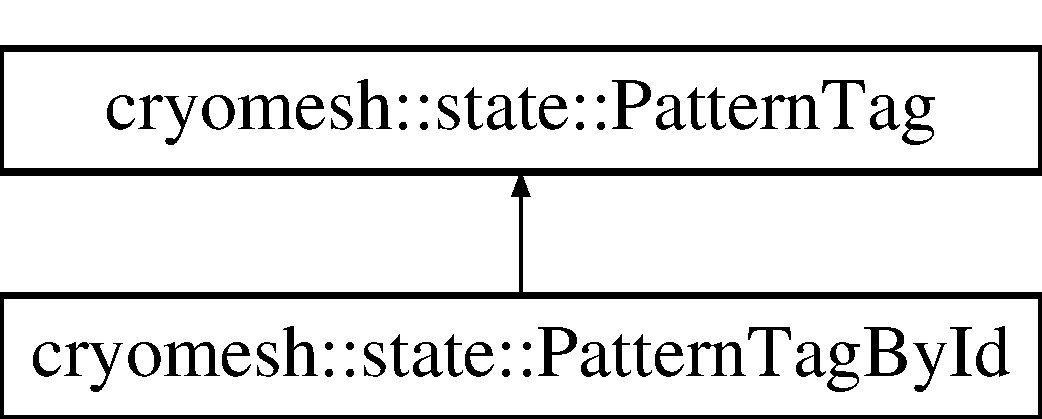
\includegraphics[height=2.000000cm]{classcryomesh_1_1state_1_1PatternTagById}
\end{center}
\end{figure}
\subsection*{\-Public \-Member \-Functions}
\begin{DoxyCompactItemize}
\item 
\hyperlink{classcryomesh_1_1state_1_1PatternTagById_a2c11f41ca6f8ab4a65fa63e250fd2660}{\-Pattern\-Tag\-By\-Id} (int d)
\item 
virtual \hyperlink{classcryomesh_1_1state_1_1PatternTagById_a67999e382d416f40ccdcb4be2d491ced}{$\sim$\-Pattern\-Tag\-By\-Id} ()
\item 
virtual std\-::string \hyperlink{classcryomesh_1_1state_1_1PatternTagById_acee63d4183580398eb30161dfbb3a88d}{get\-Tag} () const 
\item 
virtual void \hyperlink{classcryomesh_1_1state_1_1PatternTagById_a5cfba8a1a26501eb671f186c0b47ff0c}{set\-Tag} (std\-::string tg)
\item 
virtual std\-::string \hyperlink{classcryomesh_1_1state_1_1PatternTagById_aa8146b29d5b9448d9a73fde4f18c1b70}{move\-Tag} ()
\item 
virtual std\-::string \hyperlink{classcryomesh_1_1state_1_1PatternTagById_a27fb4f51f07766bd1715b5c8b31454ee}{move\-Tag} (int i)
\item 
virtual std\-::string \hyperlink{classcryomesh_1_1state_1_1PatternTagById_ac2624633ba018f4ad1ae229278cfe198}{get\-Start\-Tag} () const 
\item 
virtual std\-::string \hyperlink{classcryomesh_1_1state_1_1PatternTagById_a9d5f9cc34fd14d895ce235cea35aebe8}{get\-End\-Tag} () const 
\item 
virtual void \hyperlink{classcryomesh_1_1state_1_1PatternTagById_a9adf0ade652a4e48acd264e11e10e3b7}{set\-Start\-Tag} (std\-::string tg)
\item 
virtual void \hyperlink{classcryomesh_1_1state_1_1PatternTagById_a02e3ef3349001a9cba60cb5e0fc150cd}{set\-End\-Tag} (std\-::string tg)
\item 
virtual boost\-::shared\-\_\-ptr\*
$<$ \hyperlink{classcryomesh_1_1state_1_1PatternTag}{\-Pattern\-Tag} $>$ \hyperlink{classcryomesh_1_1state_1_1PatternTagById_ac3dbe345fe252b9ab9feafa995e91474}{get\-Global\-Tag} ()
\end{DoxyCompactItemize}
\subsection*{\-Private \-Attributes}
\begin{DoxyCompactItemize}
\item 
std\-::string \hyperlink{classcryomesh_1_1state_1_1PatternTagById_a9470fbc97fc84afd2eeae7b5e9166715}{id}
\end{DoxyCompactItemize}
\subsection*{\-Static \-Private \-Attributes}
\begin{DoxyCompactItemize}
\item 
static boost\-::shared\-\_\-ptr\*
$<$ \hyperlink{classcryomesh_1_1state_1_1PatternTagById}{\-Pattern\-Tag\-By\-Id} $>$ \hyperlink{classcryomesh_1_1state_1_1PatternTagById_a691a6ad8390ea3badf22bb88bade46cb}{global\-Tag} = boost\-::shared\-\_\-ptr$<$\hyperlink{classcryomesh_1_1state_1_1PatternTagById}{\-Pattern\-Tag\-By\-Id}$>$(new \hyperlink{classcryomesh_1_1state_1_1PatternTagById}{\-Pattern\-Tag\-By\-Id}(1))
\end{DoxyCompactItemize}


\subsection{\-Detailed \-Description}


\-Definition at line 14 of file \-Pattern\-Tag\-By\-Id.\-h.



\subsection{\-Constructor \& \-Destructor \-Documentation}
\hypertarget{classcryomesh_1_1state_1_1PatternTagById_a2c11f41ca6f8ab4a65fa63e250fd2660}{\index{cryomesh\-::state\-::\-Pattern\-Tag\-By\-Id@{cryomesh\-::state\-::\-Pattern\-Tag\-By\-Id}!\-Pattern\-Tag\-By\-Id@{\-Pattern\-Tag\-By\-Id}}
\index{\-Pattern\-Tag\-By\-Id@{\-Pattern\-Tag\-By\-Id}!cryomesh::state::PatternTagById@{cryomesh\-::state\-::\-Pattern\-Tag\-By\-Id}}
\subsubsection[{\-Pattern\-Tag\-By\-Id}]{\setlength{\rightskip}{0pt plus 5cm}{\bf cryomesh\-::state\-::\-Pattern\-Tag\-By\-Id\-::\-Pattern\-Tag\-By\-Id} (
\begin{DoxyParamCaption}
\item[{int}]{d}
\end{DoxyParamCaption}
)}}\label{classcryomesh_1_1state_1_1PatternTagById_a2c11f41ca6f8ab4a65fa63e250fd2660}


\-Definition at line 15 of file \-Pattern\-Tag\-By\-Id.\-cpp.

\hypertarget{classcryomesh_1_1state_1_1PatternTagById_a67999e382d416f40ccdcb4be2d491ced}{\index{cryomesh\-::state\-::\-Pattern\-Tag\-By\-Id@{cryomesh\-::state\-::\-Pattern\-Tag\-By\-Id}!$\sim$\-Pattern\-Tag\-By\-Id@{$\sim$\-Pattern\-Tag\-By\-Id}}
\index{$\sim$\-Pattern\-Tag\-By\-Id@{$\sim$\-Pattern\-Tag\-By\-Id}!cryomesh::state::PatternTagById@{cryomesh\-::state\-::\-Pattern\-Tag\-By\-Id}}
\subsubsection[{$\sim$\-Pattern\-Tag\-By\-Id}]{\setlength{\rightskip}{0pt plus 5cm}{\bf cryomesh\-::state\-::\-Pattern\-Tag\-By\-Id\-::$\sim$\-Pattern\-Tag\-By\-Id} (
\begin{DoxyParamCaption}
{}
\end{DoxyParamCaption}
)\hspace{0.3cm}{\ttfamily  \mbox{[}virtual\mbox{]}}}}\label{classcryomesh_1_1state_1_1PatternTagById_a67999e382d416f40ccdcb4be2d491ced}


\-Definition at line 21 of file \-Pattern\-Tag\-By\-Id.\-cpp.



\subsection{\-Member \-Function \-Documentation}
\hypertarget{classcryomesh_1_1state_1_1PatternTagById_a9d5f9cc34fd14d895ce235cea35aebe8}{\index{cryomesh\-::state\-::\-Pattern\-Tag\-By\-Id@{cryomesh\-::state\-::\-Pattern\-Tag\-By\-Id}!get\-End\-Tag@{get\-End\-Tag}}
\index{get\-End\-Tag@{get\-End\-Tag}!cryomesh::state::PatternTagById@{cryomesh\-::state\-::\-Pattern\-Tag\-By\-Id}}
\subsubsection[{get\-End\-Tag}]{\setlength{\rightskip}{0pt plus 5cm}std\-::string {\bf cryomesh\-::state\-::\-Pattern\-Tag\-By\-Id\-::get\-End\-Tag} (
\begin{DoxyParamCaption}
{}
\end{DoxyParamCaption}
) const\hspace{0.3cm}{\ttfamily  \mbox{[}virtual\mbox{]}}}}\label{classcryomesh_1_1state_1_1PatternTagById_a9d5f9cc34fd14d895ce235cea35aebe8}


\-Implements \hyperlink{classcryomesh_1_1state_1_1PatternTag_ae6a5eb0d13e5152a33de9527c66d358b}{cryomesh\-::state\-::\-Pattern\-Tag}.



\-Definition at line 43 of file \-Pattern\-Tag\-By\-Id.\-cpp.



\-References cryomesh\-::state\-::\-Pattern\-::get\-Ids().



\-Referenced by set\-End\-Tag().

\hypertarget{classcryomesh_1_1state_1_1PatternTagById_ac3dbe345fe252b9ab9feafa995e91474}{\index{cryomesh\-::state\-::\-Pattern\-Tag\-By\-Id@{cryomesh\-::state\-::\-Pattern\-Tag\-By\-Id}!get\-Global\-Tag@{get\-Global\-Tag}}
\index{get\-Global\-Tag@{get\-Global\-Tag}!cryomesh::state::PatternTagById@{cryomesh\-::state\-::\-Pattern\-Tag\-By\-Id}}
\subsubsection[{get\-Global\-Tag}]{\setlength{\rightskip}{0pt plus 5cm}boost\-::shared\-\_\-ptr$<$ {\bf \-Pattern\-Tag} $>$ {\bf cryomesh\-::state\-::\-Pattern\-Tag\-By\-Id\-::get\-Global\-Tag} (
\begin{DoxyParamCaption}
{}
\end{DoxyParamCaption}
)\hspace{0.3cm}{\ttfamily  \mbox{[}virtual\mbox{]}}}}\label{classcryomesh_1_1state_1_1PatternTagById_ac3dbe345fe252b9ab9feafa995e91474}


\-Implements \hyperlink{classcryomesh_1_1state_1_1PatternTag_ae689bd0c2045fbb30f482123adfe4657}{cryomesh\-::state\-::\-Pattern\-Tag}.



\-Definition at line 56 of file \-Pattern\-Tag\-By\-Id.\-cpp.



\-References global\-Tag.

\hypertarget{classcryomesh_1_1state_1_1PatternTagById_ac2624633ba018f4ad1ae229278cfe198}{\index{cryomesh\-::state\-::\-Pattern\-Tag\-By\-Id@{cryomesh\-::state\-::\-Pattern\-Tag\-By\-Id}!get\-Start\-Tag@{get\-Start\-Tag}}
\index{get\-Start\-Tag@{get\-Start\-Tag}!cryomesh::state::PatternTagById@{cryomesh\-::state\-::\-Pattern\-Tag\-By\-Id}}
\subsubsection[{get\-Start\-Tag}]{\setlength{\rightskip}{0pt plus 5cm}std\-::string {\bf cryomesh\-::state\-::\-Pattern\-Tag\-By\-Id\-::get\-Start\-Tag} (
\begin{DoxyParamCaption}
{}
\end{DoxyParamCaption}
) const\hspace{0.3cm}{\ttfamily  \mbox{[}virtual\mbox{]}}}}\label{classcryomesh_1_1state_1_1PatternTagById_ac2624633ba018f4ad1ae229278cfe198}


\-Implements \hyperlink{classcryomesh_1_1state_1_1PatternTag_a19284a4419275776a7277af2de158620}{cryomesh\-::state\-::\-Pattern\-Tag}.



\-Definition at line 40 of file \-Pattern\-Tag\-By\-Id.\-cpp.



\-Referenced by set\-Start\-Tag().

\hypertarget{classcryomesh_1_1state_1_1PatternTagById_acee63d4183580398eb30161dfbb3a88d}{\index{cryomesh\-::state\-::\-Pattern\-Tag\-By\-Id@{cryomesh\-::state\-::\-Pattern\-Tag\-By\-Id}!get\-Tag@{get\-Tag}}
\index{get\-Tag@{get\-Tag}!cryomesh::state::PatternTagById@{cryomesh\-::state\-::\-Pattern\-Tag\-By\-Id}}
\subsubsection[{get\-Tag}]{\setlength{\rightskip}{0pt plus 5cm}std\-::string {\bf cryomesh\-::state\-::\-Pattern\-Tag\-By\-Id\-::get\-Tag} (
\begin{DoxyParamCaption}
{}
\end{DoxyParamCaption}
) const\hspace{0.3cm}{\ttfamily  \mbox{[}virtual\mbox{]}}}}\label{classcryomesh_1_1state_1_1PatternTagById_acee63d4183580398eb30161dfbb3a88d}


\-Implements \hyperlink{classcryomesh_1_1state_1_1PatternTag_a00c56f1f6f348e51a9c02338abf3e5ab}{cryomesh\-::state\-::\-Pattern\-Tag}.



\-Definition at line 23 of file \-Pattern\-Tag\-By\-Id.\-cpp.



\-References id.



\-Referenced by move\-Tag().

\hypertarget{classcryomesh_1_1state_1_1PatternTagById_aa8146b29d5b9448d9a73fde4f18c1b70}{\index{cryomesh\-::state\-::\-Pattern\-Tag\-By\-Id@{cryomesh\-::state\-::\-Pattern\-Tag\-By\-Id}!move\-Tag@{move\-Tag}}
\index{move\-Tag@{move\-Tag}!cryomesh::state::PatternTagById@{cryomesh\-::state\-::\-Pattern\-Tag\-By\-Id}}
\subsubsection[{move\-Tag}]{\setlength{\rightskip}{0pt plus 5cm}std\-::string {\bf cryomesh\-::state\-::\-Pattern\-Tag\-By\-Id\-::move\-Tag} (
\begin{DoxyParamCaption}
{}
\end{DoxyParamCaption}
)\hspace{0.3cm}{\ttfamily  \mbox{[}virtual\mbox{]}}}}\label{classcryomesh_1_1state_1_1PatternTagById_aa8146b29d5b9448d9a73fde4f18c1b70}


\-Implements \hyperlink{classcryomesh_1_1state_1_1PatternTag_a0b22ab8e03558ed9a2370a66b67761a0}{cryomesh\-::state\-::\-Pattern\-Tag}.



\-Definition at line 29 of file \-Pattern\-Tag\-By\-Id.\-cpp.

\hypertarget{classcryomesh_1_1state_1_1PatternTagById_a27fb4f51f07766bd1715b5c8b31454ee}{\index{cryomesh\-::state\-::\-Pattern\-Tag\-By\-Id@{cryomesh\-::state\-::\-Pattern\-Tag\-By\-Id}!move\-Tag@{move\-Tag}}
\index{move\-Tag@{move\-Tag}!cryomesh::state::PatternTagById@{cryomesh\-::state\-::\-Pattern\-Tag\-By\-Id}}
\subsubsection[{move\-Tag}]{\setlength{\rightskip}{0pt plus 5cm}std\-::string {\bf cryomesh\-::state\-::\-Pattern\-Tag\-By\-Id\-::move\-Tag} (
\begin{DoxyParamCaption}
\item[{int}]{i}
\end{DoxyParamCaption}
)\hspace{0.3cm}{\ttfamily  \mbox{[}virtual\mbox{]}}}}\label{classcryomesh_1_1state_1_1PatternTagById_a27fb4f51f07766bd1715b5c8b31454ee}


\-Implements \hyperlink{classcryomesh_1_1state_1_1PatternTag_ac904d5f971af7e9930ce85a256097c48}{cryomesh\-::state\-::\-Pattern\-Tag}.



\-Definition at line 32 of file \-Pattern\-Tag\-By\-Id.\-cpp.



\-References get\-Tag().

\hypertarget{classcryomesh_1_1state_1_1PatternTagById_a02e3ef3349001a9cba60cb5e0fc150cd}{\index{cryomesh\-::state\-::\-Pattern\-Tag\-By\-Id@{cryomesh\-::state\-::\-Pattern\-Tag\-By\-Id}!set\-End\-Tag@{set\-End\-Tag}}
\index{set\-End\-Tag@{set\-End\-Tag}!cryomesh::state::PatternTagById@{cryomesh\-::state\-::\-Pattern\-Tag\-By\-Id}}
\subsubsection[{set\-End\-Tag}]{\setlength{\rightskip}{0pt plus 5cm}void {\bf cryomesh\-::state\-::\-Pattern\-Tag\-By\-Id\-::set\-End\-Tag} (
\begin{DoxyParamCaption}
\item[{std\-::string}]{tg}
\end{DoxyParamCaption}
)\hspace{0.3cm}{\ttfamily  \mbox{[}virtual\mbox{]}}}}\label{classcryomesh_1_1state_1_1PatternTagById_a02e3ef3349001a9cba60cb5e0fc150cd}


\-Implements \hyperlink{classcryomesh_1_1state_1_1PatternTag_a5026dd228cf678c58267ff343ff84e04}{cryomesh\-::state\-::\-Pattern\-Tag}.



\-Definition at line 53 of file \-Pattern\-Tag\-By\-Id.\-cpp.



\-References get\-End\-Tag().

\hypertarget{classcryomesh_1_1state_1_1PatternTagById_a9adf0ade652a4e48acd264e11e10e3b7}{\index{cryomesh\-::state\-::\-Pattern\-Tag\-By\-Id@{cryomesh\-::state\-::\-Pattern\-Tag\-By\-Id}!set\-Start\-Tag@{set\-Start\-Tag}}
\index{set\-Start\-Tag@{set\-Start\-Tag}!cryomesh::state::PatternTagById@{cryomesh\-::state\-::\-Pattern\-Tag\-By\-Id}}
\subsubsection[{set\-Start\-Tag}]{\setlength{\rightskip}{0pt plus 5cm}void {\bf cryomesh\-::state\-::\-Pattern\-Tag\-By\-Id\-::set\-Start\-Tag} (
\begin{DoxyParamCaption}
\item[{std\-::string}]{tg}
\end{DoxyParamCaption}
)\hspace{0.3cm}{\ttfamily  \mbox{[}virtual\mbox{]}}}}\label{classcryomesh_1_1state_1_1PatternTagById_a9adf0ade652a4e48acd264e11e10e3b7}


\-Implements \hyperlink{classcryomesh_1_1state_1_1PatternTag_a0c7e050117e2cc5d146b90efad122561}{cryomesh\-::state\-::\-Pattern\-Tag}.



\-Definition at line 50 of file \-Pattern\-Tag\-By\-Id.\-cpp.



\-References get\-Start\-Tag().

\hypertarget{classcryomesh_1_1state_1_1PatternTagById_a5cfba8a1a26501eb671f186c0b47ff0c}{\index{cryomesh\-::state\-::\-Pattern\-Tag\-By\-Id@{cryomesh\-::state\-::\-Pattern\-Tag\-By\-Id}!set\-Tag@{set\-Tag}}
\index{set\-Tag@{set\-Tag}!cryomesh::state::PatternTagById@{cryomesh\-::state\-::\-Pattern\-Tag\-By\-Id}}
\subsubsection[{set\-Tag}]{\setlength{\rightskip}{0pt plus 5cm}void {\bf cryomesh\-::state\-::\-Pattern\-Tag\-By\-Id\-::set\-Tag} (
\begin{DoxyParamCaption}
\item[{std\-::string}]{tg}
\end{DoxyParamCaption}
)\hspace{0.3cm}{\ttfamily  \mbox{[}virtual\mbox{]}}}}\label{classcryomesh_1_1state_1_1PatternTagById_a5cfba8a1a26501eb671f186c0b47ff0c}


\-Implements \hyperlink{classcryomesh_1_1state_1_1PatternTag_a17830f089a443437fa736460e231706e}{cryomesh\-::state\-::\-Pattern\-Tag}.



\-Definition at line 26 of file \-Pattern\-Tag\-By\-Id.\-cpp.



\subsection{\-Member \-Data \-Documentation}
\hypertarget{classcryomesh_1_1state_1_1PatternTagById_a691a6ad8390ea3badf22bb88bade46cb}{\index{cryomesh\-::state\-::\-Pattern\-Tag\-By\-Id@{cryomesh\-::state\-::\-Pattern\-Tag\-By\-Id}!global\-Tag@{global\-Tag}}
\index{global\-Tag@{global\-Tag}!cryomesh::state::PatternTagById@{cryomesh\-::state\-::\-Pattern\-Tag\-By\-Id}}
\subsubsection[{global\-Tag}]{\setlength{\rightskip}{0pt plus 5cm}boost\-::shared\-\_\-ptr$<$ {\bf \-Pattern\-Tag\-By\-Id} $>$ {\bf cryomesh\-::state\-::\-Pattern\-Tag\-By\-Id\-::global\-Tag} = boost\-::shared\-\_\-ptr$<${\bf \-Pattern\-Tag\-By\-Id}$>$(new {\bf \-Pattern\-Tag\-By\-Id}(1))\hspace{0.3cm}{\ttfamily  \mbox{[}static, private\mbox{]}}}}\label{classcryomesh_1_1state_1_1PatternTagById_a691a6ad8390ea3badf22bb88bade46cb}


\-Definition at line 29 of file \-Pattern\-Tag\-By\-Id.\-h.



\-Referenced by get\-Global\-Tag().

\hypertarget{classcryomesh_1_1state_1_1PatternTagById_a9470fbc97fc84afd2eeae7b5e9166715}{\index{cryomesh\-::state\-::\-Pattern\-Tag\-By\-Id@{cryomesh\-::state\-::\-Pattern\-Tag\-By\-Id}!id@{id}}
\index{id@{id}!cryomesh::state::PatternTagById@{cryomesh\-::state\-::\-Pattern\-Tag\-By\-Id}}
\subsubsection[{id}]{\setlength{\rightskip}{0pt plus 5cm}std\-::string {\bf cryomesh\-::state\-::\-Pattern\-Tag\-By\-Id\-::id}\hspace{0.3cm}{\ttfamily  \mbox{[}private\mbox{]}}}}\label{classcryomesh_1_1state_1_1PatternTagById_a9470fbc97fc84afd2eeae7b5e9166715}


\-Definition at line 30 of file \-Pattern\-Tag\-By\-Id.\-h.



\-Referenced by get\-Tag().



\-The documentation for this class was generated from the following files\-:\begin{DoxyCompactItemize}
\item 
/home/niall/\-Projects/\-Eclipse/\-C\-P\-P/cryomesh/src/state/\hyperlink{PatternTagById_8h}{\-Pattern\-Tag\-By\-Id.\-h}\item 
/home/niall/\-Projects/\-Eclipse/\-C\-P\-P/cryomesh/src/state/\hyperlink{PatternTagById_8cpp}{\-Pattern\-Tag\-By\-Id.\-cpp}\end{DoxyCompactItemize}

\hypertarget{structcryomesh_1_1Pointer}{\section{cryomesh\-:\-:\-Pointer$<$ \-T $>$ \-Struct \-Template \-Reference}
\label{structcryomesh_1_1Pointer}\index{cryomesh\-::\-Pointer$<$ T $>$@{cryomesh\-::\-Pointer$<$ T $>$}}
}


\hyperlink{structcryomesh_1_1Pointer}{\-Pointer} struct to allow typdef of templated smart pointers.  




{\ttfamily \#include $<$\-Defs.\-h$>$}

\subsection*{\-Public \-Types}
\begin{DoxyCompactItemize}
\item 
typedef boost\-::scoped\-\_\-ptr$<$ \-T $>$ \hyperlink{structcryomesh_1_1Pointer_a84794c15bea7c7dd8fceb679054cbdf8}{scoped\-\_\-ptr}
\item 
typedef boost\-::shared\-\_\-ptr$<$ \-T $>$ \hyperlink{structcryomesh_1_1Pointer_a825e9aaef4547bc1dd4c19424c162b89}{shared\-\_\-ptr}
\end{DoxyCompactItemize}


\subsection{\-Detailed \-Description}
\subsubsection*{template$<$class T$>$struct cryomesh\-::\-Pointer$<$ T $>$}

\hyperlink{structcryomesh_1_1Pointer}{\-Pointer} struct to allow typdef of templated smart pointers. 

\-Definition at line 23 of file \-Defs.\-h.



\subsection{\-Member \-Typedef \-Documentation}
\hypertarget{structcryomesh_1_1Pointer_a84794c15bea7c7dd8fceb679054cbdf8}{\index{cryomesh\-::\-Pointer@{cryomesh\-::\-Pointer}!scoped\-\_\-ptr@{scoped\-\_\-ptr}}
\index{scoped\-\_\-ptr@{scoped\-\_\-ptr}!cryomesh::Pointer@{cryomesh\-::\-Pointer}}
\subsubsection[{scoped\-\_\-ptr}]{\setlength{\rightskip}{0pt plus 5cm}template$<$class T $>$ typedef boost\-::scoped\-\_\-ptr$<$\-T$>$ {\bf cryomesh\-::\-Pointer}$<$ \-T $>$\-::{\bf scoped\-\_\-ptr}}}\label{structcryomesh_1_1Pointer_a84794c15bea7c7dd8fceb679054cbdf8}


\-Definition at line 28 of file \-Defs.\-h.

\hypertarget{structcryomesh_1_1Pointer_a825e9aaef4547bc1dd4c19424c162b89}{\index{cryomesh\-::\-Pointer@{cryomesh\-::\-Pointer}!shared\-\_\-ptr@{shared\-\_\-ptr}}
\index{shared\-\_\-ptr@{shared\-\_\-ptr}!cryomesh::Pointer@{cryomesh\-::\-Pointer}}
\subsubsection[{shared\-\_\-ptr}]{\setlength{\rightskip}{0pt plus 5cm}template$<$class T $>$ typedef boost\-::shared\-\_\-ptr$<$\-T$>$ {\bf cryomesh\-::\-Pointer}$<$ \-T $>$\-::{\bf shared\-\_\-ptr}}}\label{structcryomesh_1_1Pointer_a825e9aaef4547bc1dd4c19424c162b89}


\-Definition at line 29 of file \-Defs.\-h.



\-The documentation for this struct was generated from the following file\-:\begin{DoxyCompactItemize}
\item 
/home/niall/\-Projects/\-Eclipse/\-C\-P\-P/cryomesh/src/\hyperlink{Defs_8h}{\-Defs.\-h}\end{DoxyCompactItemize}

\hypertarget{structcryomesh_1_1manipulators_1_1ClusterAnalysisData_1_1RangeEnergy}{\section{cryomesh\-:\-:manipulators\-:\-:\-Cluster\-Analysis\-Data\-:\-:\-Range\-Energy \-Struct \-Reference}
\label{structcryomesh_1_1manipulators_1_1ClusterAnalysisData_1_1RangeEnergy}\index{cryomesh\-::manipulators\-::\-Cluster\-Analysis\-Data\-::\-Range\-Energy@{cryomesh\-::manipulators\-::\-Cluster\-Analysis\-Data\-::\-Range\-Energy}}
}


\-Struct representing the value extrapolated over a history range.  




{\ttfamily \#include $<$\-Cluster\-Analysis\-Data.\-h$>$}

\subsection*{\-Public \-Member \-Functions}
\begin{DoxyCompactItemize}
\item 
\hyperlink{structcryomesh_1_1manipulators_1_1ClusterAnalysisData_1_1RangeEnergy_a2b748fd0dc43023c69f702c41553aceb}{\-Range\-Energy} ()
\item 
\hyperlink{structcryomesh_1_1manipulators_1_1ClusterAnalysisData_1_1RangeEnergy_abf3ff2eb9a39171461d1137eda38f8d3}{\-Range\-Energy} (double en, double energy\-\_\-fraction)
\item 
\hyperlink{structcryomesh_1_1manipulators_1_1ClusterAnalysisData_1_1RangeEnergy_aeea4ce3ee9e2b1fdbe7e11bca5054b59}{\-Range\-Energy} (double en, double energy\-\_\-fraction, \hyperlink{classcryomesh_1_1common_1_1Cycle}{common\-::\-Cycle} st, \hyperlink{classcryomesh_1_1common_1_1Cycle}{common\-::\-Cycle} ed, double min, double max)
\item 
\hyperlink{structcryomesh_1_1manipulators_1_1ClusterAnalysisData_1_1RangeEnergy_afda1e98ceb489ddd22f557fbda270fed}{\-Range\-Energy} (const \hyperlink{structcryomesh_1_1manipulators_1_1ClusterAnalysisData_1_1RangeEnergy}{\-Range\-Energy} \&obj)
\item 
virtual \hyperlink{structcryomesh_1_1manipulators_1_1ClusterAnalysisData_1_1RangeEnergy_aa586818fb71f316d9d031cc36eec2556}{$\sim$\-Range\-Energy} ()
\item 
const \hyperlink{structcryomesh_1_1manipulators_1_1ClusterAnalysisData_1_1RangeEnergy}{\-Range\-Energy} \hyperlink{structcryomesh_1_1manipulators_1_1ClusterAnalysisData_1_1RangeEnergy_a3e872ded9405bd8e1d994d8ebbd11ef3}{operator+} (const \hyperlink{structcryomesh_1_1manipulators_1_1ClusterAnalysisData_1_1RangeEnergy}{\-Range\-Energy} \&obj) const 
\begin{DoxyCompactList}\small\item\em \-Non-\/destructive addition operator. \end{DoxyCompactList}\item 
\hyperlink{structcryomesh_1_1manipulators_1_1ClusterAnalysisData_1_1RangeEnergy}{\-Range\-Energy} \& \hyperlink{structcryomesh_1_1manipulators_1_1ClusterAnalysisData_1_1RangeEnergy_a63e6c674d7f7e89a90f88d5462279f1e}{operator+=} (const \hyperlink{structcryomesh_1_1manipulators_1_1ClusterAnalysisData_1_1RangeEnergy}{\-Range\-Energy} \&obj)
\begin{DoxyCompactList}\small\item\em \-Destructive addition and assignment operator. \end{DoxyCompactList}\item 
const \hyperlink{structcryomesh_1_1manipulators_1_1ClusterAnalysisData_1_1RangeEnergy}{\-Range\-Energy} \hyperlink{structcryomesh_1_1manipulators_1_1ClusterAnalysisData_1_1RangeEnergy_a86f0ca22060ff3039d8df9457edae402}{operator/} (double div) const 
\item 
\hyperlink{structcryomesh_1_1manipulators_1_1ClusterAnalysisData_1_1RangeEnergy}{\-Range\-Energy} \& \hyperlink{structcryomesh_1_1manipulators_1_1ClusterAnalysisData_1_1RangeEnergy_a2bc35c2465673beb91fc67d0e5c595c1}{operator/=} (double div)
\end{DoxyCompactItemize}
\subsection*{\-Public \-Attributes}
\begin{DoxyCompactItemize}
\item 
double \hyperlink{structcryomesh_1_1manipulators_1_1ClusterAnalysisData_1_1RangeEnergy_a5ec0dd8061e8109c679fb03c46175f41}{energy}
\item 
double \hyperlink{structcryomesh_1_1manipulators_1_1ClusterAnalysisData_1_1RangeEnergy_a5b00be235f5ec97fc564a87b7a53e15f}{energy\-Fraction}
\item 
\hyperlink{classcryomesh_1_1common_1_1Cycle}{common\-::\-Cycle} \hyperlink{structcryomesh_1_1manipulators_1_1ClusterAnalysisData_1_1RangeEnergy_a4160dfffe32413f76e5effce2c95ae20}{start\-Cycle}
\item 
\hyperlink{classcryomesh_1_1common_1_1Cycle}{common\-::\-Cycle} \hyperlink{structcryomesh_1_1manipulators_1_1ClusterAnalysisData_1_1RangeEnergy_afc1f6d068e8301e327981a578b83f981}{end\-Cycle}
\item 
double \hyperlink{structcryomesh_1_1manipulators_1_1ClusterAnalysisData_1_1RangeEnergy_aca92fb70884ff9717e530d91130d5e8d}{energy\-Min}
\item 
double \hyperlink{structcryomesh_1_1manipulators_1_1ClusterAnalysisData_1_1RangeEnergy_a51770c52465ceb02f9d452a46bedff77}{energy\-Max}
\end{DoxyCompactItemize}
\subsection*{\-Friends}
\begin{DoxyCompactItemize}
\item 
std\-::ostream \& \hyperlink{structcryomesh_1_1manipulators_1_1ClusterAnalysisData_1_1RangeEnergy_a99c9c1ea00dd9e77cfaa8ac83f560854}{operator$<$$<$} (std\-::ostream \&os, const \hyperlink{structcryomesh_1_1manipulators_1_1ClusterAnalysisData_1_1RangeEnergy}{\-Range\-Energy} \&obj)
\begin{DoxyCompactList}\small\item\em \-To stream operator. \end{DoxyCompactList}\end{DoxyCompactItemize}


\subsection{\-Detailed \-Description}
\-Struct representing the value extrapolated over a history range. 

\-Definition at line 24 of file \-Cluster\-Analysis\-Data.\-h.



\subsection{\-Constructor \& \-Destructor \-Documentation}
\hypertarget{structcryomesh_1_1manipulators_1_1ClusterAnalysisData_1_1RangeEnergy_a2b748fd0dc43023c69f702c41553aceb}{\index{cryomesh\-::manipulators\-::\-Cluster\-Analysis\-Data\-::\-Range\-Energy@{cryomesh\-::manipulators\-::\-Cluster\-Analysis\-Data\-::\-Range\-Energy}!\-Range\-Energy@{\-Range\-Energy}}
\index{\-Range\-Energy@{\-Range\-Energy}!cryomesh::manipulators::ClusterAnalysisData::RangeEnergy@{cryomesh\-::manipulators\-::\-Cluster\-Analysis\-Data\-::\-Range\-Energy}}
\subsubsection[{\-Range\-Energy}]{\setlength{\rightskip}{0pt plus 5cm}{\bf cryomesh\-::manipulators\-::\-Cluster\-Analysis\-Data\-::\-Range\-Energy\-::\-Range\-Energy} (
\begin{DoxyParamCaption}
{}
\end{DoxyParamCaption}
)\hspace{0.3cm}{\ttfamily  \mbox{[}inline\mbox{]}}}}\label{structcryomesh_1_1manipulators_1_1ClusterAnalysisData_1_1RangeEnergy_a2b748fd0dc43023c69f702c41553aceb}


\-Definition at line 25 of file \-Cluster\-Analysis\-Data.\-h.

\hypertarget{structcryomesh_1_1manipulators_1_1ClusterAnalysisData_1_1RangeEnergy_abf3ff2eb9a39171461d1137eda38f8d3}{\index{cryomesh\-::manipulators\-::\-Cluster\-Analysis\-Data\-::\-Range\-Energy@{cryomesh\-::manipulators\-::\-Cluster\-Analysis\-Data\-::\-Range\-Energy}!\-Range\-Energy@{\-Range\-Energy}}
\index{\-Range\-Energy@{\-Range\-Energy}!cryomesh::manipulators::ClusterAnalysisData::RangeEnergy@{cryomesh\-::manipulators\-::\-Cluster\-Analysis\-Data\-::\-Range\-Energy}}
\subsubsection[{\-Range\-Energy}]{\setlength{\rightskip}{0pt plus 5cm}{\bf cryomesh\-::manipulators\-::\-Cluster\-Analysis\-Data\-::\-Range\-Energy\-::\-Range\-Energy} (
\begin{DoxyParamCaption}
\item[{double}]{en, }
\item[{double}]{energy\-\_\-fraction}
\end{DoxyParamCaption}
)\hspace{0.3cm}{\ttfamily  \mbox{[}inline\mbox{]}}}}\label{structcryomesh_1_1manipulators_1_1ClusterAnalysisData_1_1RangeEnergy_abf3ff2eb9a39171461d1137eda38f8d3}


\-Definition at line 28 of file \-Cluster\-Analysis\-Data.\-h.

\hypertarget{structcryomesh_1_1manipulators_1_1ClusterAnalysisData_1_1RangeEnergy_aeea4ce3ee9e2b1fdbe7e11bca5054b59}{\index{cryomesh\-::manipulators\-::\-Cluster\-Analysis\-Data\-::\-Range\-Energy@{cryomesh\-::manipulators\-::\-Cluster\-Analysis\-Data\-::\-Range\-Energy}!\-Range\-Energy@{\-Range\-Energy}}
\index{\-Range\-Energy@{\-Range\-Energy}!cryomesh::manipulators::ClusterAnalysisData::RangeEnergy@{cryomesh\-::manipulators\-::\-Cluster\-Analysis\-Data\-::\-Range\-Energy}}
\subsubsection[{\-Range\-Energy}]{\setlength{\rightskip}{0pt plus 5cm}{\bf cryomesh\-::manipulators\-::\-Cluster\-Analysis\-Data\-::\-Range\-Energy\-::\-Range\-Energy} (
\begin{DoxyParamCaption}
\item[{double}]{en, }
\item[{double}]{energy\-\_\-fraction, }
\item[{{\bf common\-::\-Cycle}}]{st, }
\item[{{\bf common\-::\-Cycle}}]{ed, }
\item[{double}]{min, }
\item[{double}]{max}
\end{DoxyParamCaption}
)\hspace{0.3cm}{\ttfamily  \mbox{[}inline\mbox{]}}}}\label{structcryomesh_1_1manipulators_1_1ClusterAnalysisData_1_1RangeEnergy_aeea4ce3ee9e2b1fdbe7e11bca5054b59}


\-Definition at line 32 of file \-Cluster\-Analysis\-Data.\-h.

\hypertarget{structcryomesh_1_1manipulators_1_1ClusterAnalysisData_1_1RangeEnergy_afda1e98ceb489ddd22f557fbda270fed}{\index{cryomesh\-::manipulators\-::\-Cluster\-Analysis\-Data\-::\-Range\-Energy@{cryomesh\-::manipulators\-::\-Cluster\-Analysis\-Data\-::\-Range\-Energy}!\-Range\-Energy@{\-Range\-Energy}}
\index{\-Range\-Energy@{\-Range\-Energy}!cryomesh::manipulators::ClusterAnalysisData::RangeEnergy@{cryomesh\-::manipulators\-::\-Cluster\-Analysis\-Data\-::\-Range\-Energy}}
\subsubsection[{\-Range\-Energy}]{\setlength{\rightskip}{0pt plus 5cm}{\bf cryomesh\-::manipulators\-::\-Cluster\-Analysis\-Data\-::\-Range\-Energy\-::\-Range\-Energy} (
\begin{DoxyParamCaption}
\item[{const {\bf \-Range\-Energy} \&}]{obj}
\end{DoxyParamCaption}
)\hspace{0.3cm}{\ttfamily  \mbox{[}inline\mbox{]}}}}\label{structcryomesh_1_1manipulators_1_1ClusterAnalysisData_1_1RangeEnergy_afda1e98ceb489ddd22f557fbda270fed}


\-Definition at line 36 of file \-Cluster\-Analysis\-Data.\-h.

\hypertarget{structcryomesh_1_1manipulators_1_1ClusterAnalysisData_1_1RangeEnergy_aa586818fb71f316d9d031cc36eec2556}{\index{cryomesh\-::manipulators\-::\-Cluster\-Analysis\-Data\-::\-Range\-Energy@{cryomesh\-::manipulators\-::\-Cluster\-Analysis\-Data\-::\-Range\-Energy}!$\sim$\-Range\-Energy@{$\sim$\-Range\-Energy}}
\index{$\sim$\-Range\-Energy@{$\sim$\-Range\-Energy}!cryomesh::manipulators::ClusterAnalysisData::RangeEnergy@{cryomesh\-::manipulators\-::\-Cluster\-Analysis\-Data\-::\-Range\-Energy}}
\subsubsection[{$\sim$\-Range\-Energy}]{\setlength{\rightskip}{0pt plus 5cm}virtual {\bf cryomesh\-::manipulators\-::\-Cluster\-Analysis\-Data\-::\-Range\-Energy\-::$\sim$\-Range\-Energy} (
\begin{DoxyParamCaption}
{}
\end{DoxyParamCaption}
)\hspace{0.3cm}{\ttfamily  \mbox{[}inline, virtual\mbox{]}}}}\label{structcryomesh_1_1manipulators_1_1ClusterAnalysisData_1_1RangeEnergy_aa586818fb71f316d9d031cc36eec2556}


\-Definition at line 40 of file \-Cluster\-Analysis\-Data.\-h.



\subsection{\-Member \-Function \-Documentation}
\hypertarget{structcryomesh_1_1manipulators_1_1ClusterAnalysisData_1_1RangeEnergy_a3e872ded9405bd8e1d994d8ebbd11ef3}{\index{cryomesh\-::manipulators\-::\-Cluster\-Analysis\-Data\-::\-Range\-Energy@{cryomesh\-::manipulators\-::\-Cluster\-Analysis\-Data\-::\-Range\-Energy}!operator+@{operator+}}
\index{operator+@{operator+}!cryomesh::manipulators::ClusterAnalysisData::RangeEnergy@{cryomesh\-::manipulators\-::\-Cluster\-Analysis\-Data\-::\-Range\-Energy}}
\subsubsection[{operator+}]{\setlength{\rightskip}{0pt plus 5cm}const {\bf \-Range\-Energy} cryomesh\-::manipulators\-::\-Cluster\-Analysis\-Data\-::\-Range\-Energy\-::operator+ (
\begin{DoxyParamCaption}
\item[{const {\bf \-Range\-Energy} \&}]{obj}
\end{DoxyParamCaption}
) const\hspace{0.3cm}{\ttfamily  \mbox{[}inline\mbox{]}}}}\label{structcryomesh_1_1manipulators_1_1ClusterAnalysisData_1_1RangeEnergy_a3e872ded9405bd8e1d994d8ebbd11ef3}


\-Non-\/destructive addition operator. 


\begin{DoxyParams}{\-Parameters}
{\em const} & \hyperlink{structcryomesh_1_1manipulators_1_1ClusterAnalysisData_1_1RangeEnergy}{\-Range\-Energy} \& obj \-R\-H\-S addition\\
\hline
\end{DoxyParams}
\begin{DoxyReturn}{\-Returns}
\hyperlink{structcryomesh_1_1manipulators_1_1ClusterAnalysisData_1_1RangeEnergy}{\-Range\-Energy} \-New object after addition 
\end{DoxyReturn}


\-Definition at line 51 of file \-Cluster\-Analysis\-Data.\-h.

\hypertarget{structcryomesh_1_1manipulators_1_1ClusterAnalysisData_1_1RangeEnergy_a63e6c674d7f7e89a90f88d5462279f1e}{\index{cryomesh\-::manipulators\-::\-Cluster\-Analysis\-Data\-::\-Range\-Energy@{cryomesh\-::manipulators\-::\-Cluster\-Analysis\-Data\-::\-Range\-Energy}!operator+=@{operator+=}}
\index{operator+=@{operator+=}!cryomesh::manipulators::ClusterAnalysisData::RangeEnergy@{cryomesh\-::manipulators\-::\-Cluster\-Analysis\-Data\-::\-Range\-Energy}}
\subsubsection[{operator+=}]{\setlength{\rightskip}{0pt plus 5cm}{\bf \-Range\-Energy}\& cryomesh\-::manipulators\-::\-Cluster\-Analysis\-Data\-::\-Range\-Energy\-::operator+= (
\begin{DoxyParamCaption}
\item[{const {\bf \-Range\-Energy} \&}]{obj}
\end{DoxyParamCaption}
)\hspace{0.3cm}{\ttfamily  \mbox{[}inline\mbox{]}}}}\label{structcryomesh_1_1manipulators_1_1ClusterAnalysisData_1_1RangeEnergy_a63e6c674d7f7e89a90f88d5462279f1e}


\-Destructive addition and assignment operator. 


\begin{DoxyParams}{\-Parameters}
{\em const} & \hyperlink{structcryomesh_1_1manipulators_1_1ClusterAnalysisData_1_1RangeEnergy}{\-Range\-Energy} \& obj \-R\-H\-S addition\\
\hline
\end{DoxyParams}
\begin{DoxyReturn}{\-Returns}
\hyperlink{structcryomesh_1_1manipulators_1_1ClusterAnalysisData_1_1RangeEnergy}{\-Range\-Energy} \& \-This object after addition and assignment 
\end{DoxyReturn}


\-Definition at line 65 of file \-Cluster\-Analysis\-Data.\-h.



\-References end\-Cycle, energy, energy\-Max, energy\-Min, and start\-Cycle.

\hypertarget{structcryomesh_1_1manipulators_1_1ClusterAnalysisData_1_1RangeEnergy_a86f0ca22060ff3039d8df9457edae402}{\index{cryomesh\-::manipulators\-::\-Cluster\-Analysis\-Data\-::\-Range\-Energy@{cryomesh\-::manipulators\-::\-Cluster\-Analysis\-Data\-::\-Range\-Energy}!operator/@{operator/}}
\index{operator/@{operator/}!cryomesh::manipulators::ClusterAnalysisData::RangeEnergy@{cryomesh\-::manipulators\-::\-Cluster\-Analysis\-Data\-::\-Range\-Energy}}
\subsubsection[{operator/}]{\setlength{\rightskip}{0pt plus 5cm}const {\bf \-Range\-Energy} cryomesh\-::manipulators\-::\-Cluster\-Analysis\-Data\-::\-Range\-Energy\-::operator/ (
\begin{DoxyParamCaption}
\item[{double}]{div}
\end{DoxyParamCaption}
) const\hspace{0.3cm}{\ttfamily  \mbox{[}inline\mbox{]}}}}\label{structcryomesh_1_1manipulators_1_1ClusterAnalysisData_1_1RangeEnergy_a86f0ca22060ff3039d8df9457edae402}


\-Definition at line 75 of file \-Cluster\-Analysis\-Data.\-h.

\hypertarget{structcryomesh_1_1manipulators_1_1ClusterAnalysisData_1_1RangeEnergy_a2bc35c2465673beb91fc67d0e5c595c1}{\index{cryomesh\-::manipulators\-::\-Cluster\-Analysis\-Data\-::\-Range\-Energy@{cryomesh\-::manipulators\-::\-Cluster\-Analysis\-Data\-::\-Range\-Energy}!operator/=@{operator/=}}
\index{operator/=@{operator/=}!cryomesh::manipulators::ClusterAnalysisData::RangeEnergy@{cryomesh\-::manipulators\-::\-Cluster\-Analysis\-Data\-::\-Range\-Energy}}
\subsubsection[{operator/=}]{\setlength{\rightskip}{0pt plus 5cm}{\bf \-Range\-Energy}\& cryomesh\-::manipulators\-::\-Cluster\-Analysis\-Data\-::\-Range\-Energy\-::operator/= (
\begin{DoxyParamCaption}
\item[{double}]{div}
\end{DoxyParamCaption}
)\hspace{0.3cm}{\ttfamily  \mbox{[}inline\mbox{]}}}}\label{structcryomesh_1_1manipulators_1_1ClusterAnalysisData_1_1RangeEnergy_a2bc35c2465673beb91fc67d0e5c595c1}


\-Definition at line 80 of file \-Cluster\-Analysis\-Data.\-h.



\-References energy.



\subsection{\-Friends \-And \-Related \-Function \-Documentation}
\hypertarget{structcryomesh_1_1manipulators_1_1ClusterAnalysisData_1_1RangeEnergy_a99c9c1ea00dd9e77cfaa8ac83f560854}{\index{cryomesh\-::manipulators\-::\-Cluster\-Analysis\-Data\-::\-Range\-Energy@{cryomesh\-::manipulators\-::\-Cluster\-Analysis\-Data\-::\-Range\-Energy}!operator$<$$<$@{operator$<$$<$}}
\index{operator$<$$<$@{operator$<$$<$}!cryomesh::manipulators::ClusterAnalysisData::RangeEnergy@{cryomesh\-::manipulators\-::\-Cluster\-Analysis\-Data\-::\-Range\-Energy}}
\subsubsection[{operator$<$$<$}]{\setlength{\rightskip}{0pt plus 5cm}std\-::ostream\& operator$<$$<$ (
\begin{DoxyParamCaption}
\item[{std\-::ostream \&}]{os, }
\item[{const {\bf \-Range\-Energy} \&}]{obj}
\end{DoxyParamCaption}
)\hspace{0.3cm}{\ttfamily  \mbox{[}friend\mbox{]}}}}\label{structcryomesh_1_1manipulators_1_1ClusterAnalysisData_1_1RangeEnergy_a99c9c1ea00dd9e77cfaa8ac83f560854}


\-To stream operator. 


\begin{DoxyParams}{\-Parameters}
{\em std\-::ostream} & \& os \-The output stream \\
\hline
{\em const} & \hyperlink{structcryomesh_1_1manipulators_1_1ClusterAnalysisData_1_1RangeEnergy}{\-Range\-Energy} \& obj \-The object to stream\\
\hline
\end{DoxyParams}
\begin{DoxyReturn}{\-Returns}
std\-::ostream \& \-The output stream 
\end{DoxyReturn}


\-Definition at line 96 of file \-Cluster\-Analysis\-Data.\-h.



\subsection{\-Member \-Data \-Documentation}
\hypertarget{structcryomesh_1_1manipulators_1_1ClusterAnalysisData_1_1RangeEnergy_afc1f6d068e8301e327981a578b83f981}{\index{cryomesh\-::manipulators\-::\-Cluster\-Analysis\-Data\-::\-Range\-Energy@{cryomesh\-::manipulators\-::\-Cluster\-Analysis\-Data\-::\-Range\-Energy}!end\-Cycle@{end\-Cycle}}
\index{end\-Cycle@{end\-Cycle}!cryomesh::manipulators::ClusterAnalysisData::RangeEnergy@{cryomesh\-::manipulators\-::\-Cluster\-Analysis\-Data\-::\-Range\-Energy}}
\subsubsection[{end\-Cycle}]{\setlength{\rightskip}{0pt plus 5cm}{\bf common\-::\-Cycle} {\bf cryomesh\-::manipulators\-::\-Cluster\-Analysis\-Data\-::\-Range\-Energy\-::end\-Cycle}}}\label{structcryomesh_1_1manipulators_1_1ClusterAnalysisData_1_1RangeEnergy_afc1f6d068e8301e327981a578b83f981}


\-Definition at line 104 of file \-Cluster\-Analysis\-Data.\-h.



\-Referenced by operator+=().

\hypertarget{structcryomesh_1_1manipulators_1_1ClusterAnalysisData_1_1RangeEnergy_a5ec0dd8061e8109c679fb03c46175f41}{\index{cryomesh\-::manipulators\-::\-Cluster\-Analysis\-Data\-::\-Range\-Energy@{cryomesh\-::manipulators\-::\-Cluster\-Analysis\-Data\-::\-Range\-Energy}!energy@{energy}}
\index{energy@{energy}!cryomesh::manipulators::ClusterAnalysisData::RangeEnergy@{cryomesh\-::manipulators\-::\-Cluster\-Analysis\-Data\-::\-Range\-Energy}}
\subsubsection[{energy}]{\setlength{\rightskip}{0pt plus 5cm}double {\bf cryomesh\-::manipulators\-::\-Cluster\-Analysis\-Data\-::\-Range\-Energy\-::energy}}}\label{structcryomesh_1_1manipulators_1_1ClusterAnalysisData_1_1RangeEnergy_a5ec0dd8061e8109c679fb03c46175f41}


\-Definition at line 101 of file \-Cluster\-Analysis\-Data.\-h.



\-Referenced by operator+=(), and operator/=().

\hypertarget{structcryomesh_1_1manipulators_1_1ClusterAnalysisData_1_1RangeEnergy_a5b00be235f5ec97fc564a87b7a53e15f}{\index{cryomesh\-::manipulators\-::\-Cluster\-Analysis\-Data\-::\-Range\-Energy@{cryomesh\-::manipulators\-::\-Cluster\-Analysis\-Data\-::\-Range\-Energy}!energy\-Fraction@{energy\-Fraction}}
\index{energy\-Fraction@{energy\-Fraction}!cryomesh::manipulators::ClusterAnalysisData::RangeEnergy@{cryomesh\-::manipulators\-::\-Cluster\-Analysis\-Data\-::\-Range\-Energy}}
\subsubsection[{energy\-Fraction}]{\setlength{\rightskip}{0pt plus 5cm}double {\bf cryomesh\-::manipulators\-::\-Cluster\-Analysis\-Data\-::\-Range\-Energy\-::energy\-Fraction}}}\label{structcryomesh_1_1manipulators_1_1ClusterAnalysisData_1_1RangeEnergy_a5b00be235f5ec97fc564a87b7a53e15f}


\-Definition at line 102 of file \-Cluster\-Analysis\-Data.\-h.



\-Referenced by cryomesh\-::manipulators\-::\-Cluster\-Analyser\-Basic\-::analyse\-Cluster().

\hypertarget{structcryomesh_1_1manipulators_1_1ClusterAnalysisData_1_1RangeEnergy_a51770c52465ceb02f9d452a46bedff77}{\index{cryomesh\-::manipulators\-::\-Cluster\-Analysis\-Data\-::\-Range\-Energy@{cryomesh\-::manipulators\-::\-Cluster\-Analysis\-Data\-::\-Range\-Energy}!energy\-Max@{energy\-Max}}
\index{energy\-Max@{energy\-Max}!cryomesh::manipulators::ClusterAnalysisData::RangeEnergy@{cryomesh\-::manipulators\-::\-Cluster\-Analysis\-Data\-::\-Range\-Energy}}
\subsubsection[{energy\-Max}]{\setlength{\rightskip}{0pt plus 5cm}double {\bf cryomesh\-::manipulators\-::\-Cluster\-Analysis\-Data\-::\-Range\-Energy\-::energy\-Max}}}\label{structcryomesh_1_1manipulators_1_1ClusterAnalysisData_1_1RangeEnergy_a51770c52465ceb02f9d452a46bedff77}


\-Definition at line 106 of file \-Cluster\-Analysis\-Data.\-h.



\-Referenced by operator+=().

\hypertarget{structcryomesh_1_1manipulators_1_1ClusterAnalysisData_1_1RangeEnergy_aca92fb70884ff9717e530d91130d5e8d}{\index{cryomesh\-::manipulators\-::\-Cluster\-Analysis\-Data\-::\-Range\-Energy@{cryomesh\-::manipulators\-::\-Cluster\-Analysis\-Data\-::\-Range\-Energy}!energy\-Min@{energy\-Min}}
\index{energy\-Min@{energy\-Min}!cryomesh::manipulators::ClusterAnalysisData::RangeEnergy@{cryomesh\-::manipulators\-::\-Cluster\-Analysis\-Data\-::\-Range\-Energy}}
\subsubsection[{energy\-Min}]{\setlength{\rightskip}{0pt plus 5cm}double {\bf cryomesh\-::manipulators\-::\-Cluster\-Analysis\-Data\-::\-Range\-Energy\-::energy\-Min}}}\label{structcryomesh_1_1manipulators_1_1ClusterAnalysisData_1_1RangeEnergy_aca92fb70884ff9717e530d91130d5e8d}


\-Definition at line 105 of file \-Cluster\-Analysis\-Data.\-h.



\-Referenced by operator+=().

\hypertarget{structcryomesh_1_1manipulators_1_1ClusterAnalysisData_1_1RangeEnergy_a4160dfffe32413f76e5effce2c95ae20}{\index{cryomesh\-::manipulators\-::\-Cluster\-Analysis\-Data\-::\-Range\-Energy@{cryomesh\-::manipulators\-::\-Cluster\-Analysis\-Data\-::\-Range\-Energy}!start\-Cycle@{start\-Cycle}}
\index{start\-Cycle@{start\-Cycle}!cryomesh::manipulators::ClusterAnalysisData::RangeEnergy@{cryomesh\-::manipulators\-::\-Cluster\-Analysis\-Data\-::\-Range\-Energy}}
\subsubsection[{start\-Cycle}]{\setlength{\rightskip}{0pt plus 5cm}{\bf common\-::\-Cycle} {\bf cryomesh\-::manipulators\-::\-Cluster\-Analysis\-Data\-::\-Range\-Energy\-::start\-Cycle}}}\label{structcryomesh_1_1manipulators_1_1ClusterAnalysisData_1_1RangeEnergy_a4160dfffe32413f76e5effce2c95ae20}


\-Definition at line 103 of file \-Cluster\-Analysis\-Data.\-h.



\-Referenced by operator+=().



\-The documentation for this struct was generated from the following file\-:\begin{DoxyCompactItemize}
\item 
/home/niall/\-Projects/\-Eclipse/\-C\-P\-P/cryomesh/src/manipulators/\hyperlink{ClusterAnalysisData_8h}{\-Cluster\-Analysis\-Data.\-h}\end{DoxyCompactItemize}

\hypertarget{structcryomesh_1_1manipulators_1_1IClusterAnalyser_1_1RestructuringCountdown}{\section{cryomesh\-:\-:manipulators\-:\-:\-I\-Cluster\-Analyser\-:\-:\-Restructuring\-Countdown \-Struct \-Reference}
\label{structcryomesh_1_1manipulators_1_1IClusterAnalyser_1_1RestructuringCountdown}\index{cryomesh\-::manipulators\-::\-I\-Cluster\-Analyser\-::\-Restructuring\-Countdown@{cryomesh\-::manipulators\-::\-I\-Cluster\-Analyser\-::\-Restructuring\-Countdown}}
}


\-Class to hold together information on whether we can act to restructure items.  




{\ttfamily \#include $<$\-I\-Cluster\-Analyser.\-h$>$}

\subsection*{\-Public \-Member \-Functions}
\begin{DoxyCompactItemize}
\item 
\hyperlink{structcryomesh_1_1manipulators_1_1IClusterAnalyser_1_1RestructuringCountdown_a404e441b64f2b4aa90b02e337d8cd804}{\-Restructuring\-Countdown} (int ct=0)
\item 
bool \hyperlink{structcryomesh_1_1manipulators_1_1IClusterAnalyser_1_1RestructuringCountdown_aa5914738b7868c568f152250cdbbe898}{is\-Restructuring\-Enabled} (int var) const 
\item 
bool \hyperlink{structcryomesh_1_1manipulators_1_1IClusterAnalyser_1_1RestructuringCountdown_a78a6c5da890ad27a0b2a5c6c3b814fd4}{is\-Any\-Short\-Restructuring\-Enabled} () const 
\item 
bool \hyperlink{structcryomesh_1_1manipulators_1_1IClusterAnalyser_1_1RestructuringCountdown_a8b9e3f9ae224384f54082495e00584f0}{is\-Any\-Medium\-Restructuring\-Enabled} () const 
\item 
bool \hyperlink{structcryomesh_1_1manipulators_1_1IClusterAnalyser_1_1RestructuringCountdown_a52d7fee545d90460bbd663798338c759}{is\-Any\-Long\-Restructuring\-Enabled} () const 
\item 
bool \hyperlink{structcryomesh_1_1manipulators_1_1IClusterAnalyser_1_1RestructuringCountdown_a0ea210cdc9eeb6770c062a9729df1104}{is\-Any\-Restructuring\-Enabled} () const 
\item 
bool \hyperlink{structcryomesh_1_1manipulators_1_1IClusterAnalyser_1_1RestructuringCountdown_ac604df5d1355de5ad42ba95a3f63ba57}{is\-All\-Short\-Restructuring\-Enabled} () const 
\item 
bool \hyperlink{structcryomesh_1_1manipulators_1_1IClusterAnalyser_1_1RestructuringCountdown_ab1c0206253593ec5cdaff55432674416}{is\-All\-Medium\-Restructuring\-Enabled} () const 
\item 
bool \hyperlink{structcryomesh_1_1manipulators_1_1IClusterAnalyser_1_1RestructuringCountdown_a11f332249883a3272c5f0cb94cf7b756}{is\-All\-Long\-Restructuring\-Enabled} () const 
\item 
bool \hyperlink{structcryomesh_1_1manipulators_1_1IClusterAnalyser_1_1RestructuringCountdown_aae17ff29ace2561d4ebbce28e9332bca}{is\-All\-Restructuring\-Enabled} () const 
\item 
\hyperlink{structcryomesh_1_1manipulators_1_1IClusterAnalyser_1_1RestructuringCountdown}{\-Restructuring\-Countdown} \& \hyperlink{structcryomesh_1_1manipulators_1_1IClusterAnalyser_1_1RestructuringCountdown_a10e256d5dd68a5d92a4eab35651920d4}{operator-\/-\/} ()
\begin{DoxyCompactList}\small\item\em \-Prefix decrement operator. \end{DoxyCompactList}\item 
void \hyperlink{structcryomesh_1_1manipulators_1_1IClusterAnalyser_1_1RestructuringCountdown_a16766b635831bbff21aaae1417cd8c2b}{set\-Short\-Countdown} (int ct)
\item 
void \hyperlink{structcryomesh_1_1manipulators_1_1IClusterAnalyser_1_1RestructuringCountdown_ab8c08d4d9dd8fd3a7ad535a7bdf3c74a}{set\-Medium\-Countdown} (int ct)
\item 
void \hyperlink{structcryomesh_1_1manipulators_1_1IClusterAnalyser_1_1RestructuringCountdown_aca25ee4c4f6a08391ab3f5fa60ea8a54}{set\-Long\-Countdown} (int ct)
\end{DoxyCompactItemize}
\subsection*{\-Public \-Attributes}
\begin{DoxyCompactItemize}
\item 
int \hyperlink{structcryomesh_1_1manipulators_1_1IClusterAnalyser_1_1RestructuringCountdown_a4e0fb0eb08819e98beb74f9ceda06964}{short\-Creation}
\item 
int \hyperlink{structcryomesh_1_1manipulators_1_1IClusterAnalyser_1_1RestructuringCountdown_aa4c23b58d7bdbdc1e6ffa1161cfa0da2}{short\-Destruction}
\item 
int \hyperlink{structcryomesh_1_1manipulators_1_1IClusterAnalyser_1_1RestructuringCountdown_ad67471fc6daa6384e77d4e6681decce5}{medium\-Creation}
\item 
int \hyperlink{structcryomesh_1_1manipulators_1_1IClusterAnalyser_1_1RestructuringCountdown_ae6adfde336b7d67ad433991af81652b4}{medium\-Destruction}
\item 
int \hyperlink{structcryomesh_1_1manipulators_1_1IClusterAnalyser_1_1RestructuringCountdown_ac248eef511236bbb0c9d5e6b454a97a3}{long\-Creation}
\item 
int \hyperlink{structcryomesh_1_1manipulators_1_1IClusterAnalyser_1_1RestructuringCountdown_a147c9ec6f5896ca4e8151e01eb764d0e}{long\-Destruction}
\end{DoxyCompactItemize}
\subsection*{\-Friends}
\begin{DoxyCompactItemize}
\item 
std\-::ostream \& \hyperlink{structcryomesh_1_1manipulators_1_1IClusterAnalyser_1_1RestructuringCountdown_afd20f7f5eb07d5e2bb273737fe91adfd}{operator$<$$<$} (std\-::ostream \&os, const \hyperlink{structcryomesh_1_1manipulators_1_1IClusterAnalyser_1_1RestructuringCountdown}{\-Restructuring\-Countdown} \&obj)
\begin{DoxyCompactList}\small\item\em \-To stream operator. \end{DoxyCompactList}\end{DoxyCompactItemize}


\subsection{\-Detailed \-Description}
\-Class to hold together information on whether we can act to restructure items. 

\-Definition at line 23 of file \-I\-Cluster\-Analyser.\-h.



\subsection{\-Constructor \& \-Destructor \-Documentation}
\hypertarget{structcryomesh_1_1manipulators_1_1IClusterAnalyser_1_1RestructuringCountdown_a404e441b64f2b4aa90b02e337d8cd804}{\index{cryomesh\-::manipulators\-::\-I\-Cluster\-Analyser\-::\-Restructuring\-Countdown@{cryomesh\-::manipulators\-::\-I\-Cluster\-Analyser\-::\-Restructuring\-Countdown}!\-Restructuring\-Countdown@{\-Restructuring\-Countdown}}
\index{\-Restructuring\-Countdown@{\-Restructuring\-Countdown}!cryomesh::manipulators::IClusterAnalyser::RestructuringCountdown@{cryomesh\-::manipulators\-::\-I\-Cluster\-Analyser\-::\-Restructuring\-Countdown}}
\subsubsection[{\-Restructuring\-Countdown}]{\setlength{\rightskip}{0pt plus 5cm}{\bf cryomesh\-::manipulators\-::\-I\-Cluster\-Analyser\-::\-Restructuring\-Countdown\-::\-Restructuring\-Countdown} (
\begin{DoxyParamCaption}
\item[{int}]{ct = {\ttfamily 0}}
\end{DoxyParamCaption}
)\hspace{0.3cm}{\ttfamily  \mbox{[}inline\mbox{]}}}}\label{structcryomesh_1_1manipulators_1_1IClusterAnalyser_1_1RestructuringCountdown_a404e441b64f2b4aa90b02e337d8cd804}


\-Definition at line 24 of file \-I\-Cluster\-Analyser.\-h.



\subsection{\-Member \-Function \-Documentation}
\hypertarget{structcryomesh_1_1manipulators_1_1IClusterAnalyser_1_1RestructuringCountdown_a11f332249883a3272c5f0cb94cf7b756}{\index{cryomesh\-::manipulators\-::\-I\-Cluster\-Analyser\-::\-Restructuring\-Countdown@{cryomesh\-::manipulators\-::\-I\-Cluster\-Analyser\-::\-Restructuring\-Countdown}!is\-All\-Long\-Restructuring\-Enabled@{is\-All\-Long\-Restructuring\-Enabled}}
\index{is\-All\-Long\-Restructuring\-Enabled@{is\-All\-Long\-Restructuring\-Enabled}!cryomesh::manipulators::IClusterAnalyser::RestructuringCountdown@{cryomesh\-::manipulators\-::\-I\-Cluster\-Analyser\-::\-Restructuring\-Countdown}}
\subsubsection[{is\-All\-Long\-Restructuring\-Enabled}]{\setlength{\rightskip}{0pt plus 5cm}bool {\bf cryomesh\-::manipulators\-::\-I\-Cluster\-Analyser\-::\-Restructuring\-Countdown\-::is\-All\-Long\-Restructuring\-Enabled} (
\begin{DoxyParamCaption}
{}
\end{DoxyParamCaption}
) const\hspace{0.3cm}{\ttfamily  \mbox{[}inline\mbox{]}}}}\label{structcryomesh_1_1manipulators_1_1IClusterAnalyser_1_1RestructuringCountdown_a11f332249883a3272c5f0cb94cf7b756}


\-Definition at line 60 of file \-I\-Cluster\-Analyser.\-h.



\-References is\-Restructuring\-Enabled(), long\-Creation, and long\-Destruction.

\hypertarget{structcryomesh_1_1manipulators_1_1IClusterAnalyser_1_1RestructuringCountdown_ab1c0206253593ec5cdaff55432674416}{\index{cryomesh\-::manipulators\-::\-I\-Cluster\-Analyser\-::\-Restructuring\-Countdown@{cryomesh\-::manipulators\-::\-I\-Cluster\-Analyser\-::\-Restructuring\-Countdown}!is\-All\-Medium\-Restructuring\-Enabled@{is\-All\-Medium\-Restructuring\-Enabled}}
\index{is\-All\-Medium\-Restructuring\-Enabled@{is\-All\-Medium\-Restructuring\-Enabled}!cryomesh::manipulators::IClusterAnalyser::RestructuringCountdown@{cryomesh\-::manipulators\-::\-I\-Cluster\-Analyser\-::\-Restructuring\-Countdown}}
\subsubsection[{is\-All\-Medium\-Restructuring\-Enabled}]{\setlength{\rightskip}{0pt plus 5cm}bool {\bf cryomesh\-::manipulators\-::\-I\-Cluster\-Analyser\-::\-Restructuring\-Countdown\-::is\-All\-Medium\-Restructuring\-Enabled} (
\begin{DoxyParamCaption}
{}
\end{DoxyParamCaption}
) const\hspace{0.3cm}{\ttfamily  \mbox{[}inline\mbox{]}}}}\label{structcryomesh_1_1manipulators_1_1IClusterAnalyser_1_1RestructuringCountdown_ab1c0206253593ec5cdaff55432674416}


\-Definition at line 56 of file \-I\-Cluster\-Analyser.\-h.



\-References is\-Restructuring\-Enabled(), medium\-Creation, and medium\-Destruction.

\hypertarget{structcryomesh_1_1manipulators_1_1IClusterAnalyser_1_1RestructuringCountdown_aae17ff29ace2561d4ebbce28e9332bca}{\index{cryomesh\-::manipulators\-::\-I\-Cluster\-Analyser\-::\-Restructuring\-Countdown@{cryomesh\-::manipulators\-::\-I\-Cluster\-Analyser\-::\-Restructuring\-Countdown}!is\-All\-Restructuring\-Enabled@{is\-All\-Restructuring\-Enabled}}
\index{is\-All\-Restructuring\-Enabled@{is\-All\-Restructuring\-Enabled}!cryomesh::manipulators::IClusterAnalyser::RestructuringCountdown@{cryomesh\-::manipulators\-::\-I\-Cluster\-Analyser\-::\-Restructuring\-Countdown}}
\subsubsection[{is\-All\-Restructuring\-Enabled}]{\setlength{\rightskip}{0pt plus 5cm}bool {\bf cryomesh\-::manipulators\-::\-I\-Cluster\-Analyser\-::\-Restructuring\-Countdown\-::is\-All\-Restructuring\-Enabled} (
\begin{DoxyParamCaption}
{}
\end{DoxyParamCaption}
) const\hspace{0.3cm}{\ttfamily  \mbox{[}inline\mbox{]}}}}\label{structcryomesh_1_1manipulators_1_1IClusterAnalyser_1_1RestructuringCountdown_aae17ff29ace2561d4ebbce28e9332bca}


\-Definition at line 64 of file \-I\-Cluster\-Analyser.\-h.



\-References is\-Any\-Long\-Restructuring\-Enabled(), is\-Any\-Medium\-Restructuring\-Enabled(), and is\-Any\-Short\-Restructuring\-Enabled().

\hypertarget{structcryomesh_1_1manipulators_1_1IClusterAnalyser_1_1RestructuringCountdown_ac604df5d1355de5ad42ba95a3f63ba57}{\index{cryomesh\-::manipulators\-::\-I\-Cluster\-Analyser\-::\-Restructuring\-Countdown@{cryomesh\-::manipulators\-::\-I\-Cluster\-Analyser\-::\-Restructuring\-Countdown}!is\-All\-Short\-Restructuring\-Enabled@{is\-All\-Short\-Restructuring\-Enabled}}
\index{is\-All\-Short\-Restructuring\-Enabled@{is\-All\-Short\-Restructuring\-Enabled}!cryomesh::manipulators::IClusterAnalyser::RestructuringCountdown@{cryomesh\-::manipulators\-::\-I\-Cluster\-Analyser\-::\-Restructuring\-Countdown}}
\subsubsection[{is\-All\-Short\-Restructuring\-Enabled}]{\setlength{\rightskip}{0pt plus 5cm}bool {\bf cryomesh\-::manipulators\-::\-I\-Cluster\-Analyser\-::\-Restructuring\-Countdown\-::is\-All\-Short\-Restructuring\-Enabled} (
\begin{DoxyParamCaption}
{}
\end{DoxyParamCaption}
) const\hspace{0.3cm}{\ttfamily  \mbox{[}inline\mbox{]}}}}\label{structcryomesh_1_1manipulators_1_1IClusterAnalyser_1_1RestructuringCountdown_ac604df5d1355de5ad42ba95a3f63ba57}


\-Definition at line 52 of file \-I\-Cluster\-Analyser.\-h.



\-References is\-Restructuring\-Enabled(), short\-Creation, and short\-Destruction.

\hypertarget{structcryomesh_1_1manipulators_1_1IClusterAnalyser_1_1RestructuringCountdown_a52d7fee545d90460bbd663798338c759}{\index{cryomesh\-::manipulators\-::\-I\-Cluster\-Analyser\-::\-Restructuring\-Countdown@{cryomesh\-::manipulators\-::\-I\-Cluster\-Analyser\-::\-Restructuring\-Countdown}!is\-Any\-Long\-Restructuring\-Enabled@{is\-Any\-Long\-Restructuring\-Enabled}}
\index{is\-Any\-Long\-Restructuring\-Enabled@{is\-Any\-Long\-Restructuring\-Enabled}!cryomesh::manipulators::IClusterAnalyser::RestructuringCountdown@{cryomesh\-::manipulators\-::\-I\-Cluster\-Analyser\-::\-Restructuring\-Countdown}}
\subsubsection[{is\-Any\-Long\-Restructuring\-Enabled}]{\setlength{\rightskip}{0pt plus 5cm}bool {\bf cryomesh\-::manipulators\-::\-I\-Cluster\-Analyser\-::\-Restructuring\-Countdown\-::is\-Any\-Long\-Restructuring\-Enabled} (
\begin{DoxyParamCaption}
{}
\end{DoxyParamCaption}
) const\hspace{0.3cm}{\ttfamily  \mbox{[}inline\mbox{]}}}}\label{structcryomesh_1_1manipulators_1_1IClusterAnalyser_1_1RestructuringCountdown_a52d7fee545d90460bbd663798338c759}


\-Definition at line 43 of file \-I\-Cluster\-Analyser.\-h.



\-References is\-Restructuring\-Enabled(), long\-Creation, and long\-Destruction.



\-Referenced by cryomesh\-::manipulators\-::\-Cluster\-Analyser\-Basic\-::analyse\-Cluster(), is\-All\-Restructuring\-Enabled(), and is\-Any\-Restructuring\-Enabled().

\hypertarget{structcryomesh_1_1manipulators_1_1IClusterAnalyser_1_1RestructuringCountdown_a8b9e3f9ae224384f54082495e00584f0}{\index{cryomesh\-::manipulators\-::\-I\-Cluster\-Analyser\-::\-Restructuring\-Countdown@{cryomesh\-::manipulators\-::\-I\-Cluster\-Analyser\-::\-Restructuring\-Countdown}!is\-Any\-Medium\-Restructuring\-Enabled@{is\-Any\-Medium\-Restructuring\-Enabled}}
\index{is\-Any\-Medium\-Restructuring\-Enabled@{is\-Any\-Medium\-Restructuring\-Enabled}!cryomesh::manipulators::IClusterAnalyser::RestructuringCountdown@{cryomesh\-::manipulators\-::\-I\-Cluster\-Analyser\-::\-Restructuring\-Countdown}}
\subsubsection[{is\-Any\-Medium\-Restructuring\-Enabled}]{\setlength{\rightskip}{0pt plus 5cm}bool {\bf cryomesh\-::manipulators\-::\-I\-Cluster\-Analyser\-::\-Restructuring\-Countdown\-::is\-Any\-Medium\-Restructuring\-Enabled} (
\begin{DoxyParamCaption}
{}
\end{DoxyParamCaption}
) const\hspace{0.3cm}{\ttfamily  \mbox{[}inline\mbox{]}}}}\label{structcryomesh_1_1manipulators_1_1IClusterAnalyser_1_1RestructuringCountdown_a8b9e3f9ae224384f54082495e00584f0}


\-Definition at line 39 of file \-I\-Cluster\-Analyser.\-h.



\-References is\-Restructuring\-Enabled(), medium\-Creation, and medium\-Destruction.



\-Referenced by cryomesh\-::manipulators\-::\-Cluster\-Analyser\-Basic\-::analyse\-Cluster(), is\-All\-Restructuring\-Enabled(), and is\-Any\-Restructuring\-Enabled().

\hypertarget{structcryomesh_1_1manipulators_1_1IClusterAnalyser_1_1RestructuringCountdown_a0ea210cdc9eeb6770c062a9729df1104}{\index{cryomesh\-::manipulators\-::\-I\-Cluster\-Analyser\-::\-Restructuring\-Countdown@{cryomesh\-::manipulators\-::\-I\-Cluster\-Analyser\-::\-Restructuring\-Countdown}!is\-Any\-Restructuring\-Enabled@{is\-Any\-Restructuring\-Enabled}}
\index{is\-Any\-Restructuring\-Enabled@{is\-Any\-Restructuring\-Enabled}!cryomesh::manipulators::IClusterAnalyser::RestructuringCountdown@{cryomesh\-::manipulators\-::\-I\-Cluster\-Analyser\-::\-Restructuring\-Countdown}}
\subsubsection[{is\-Any\-Restructuring\-Enabled}]{\setlength{\rightskip}{0pt plus 5cm}bool {\bf cryomesh\-::manipulators\-::\-I\-Cluster\-Analyser\-::\-Restructuring\-Countdown\-::is\-Any\-Restructuring\-Enabled} (
\begin{DoxyParamCaption}
{}
\end{DoxyParamCaption}
) const\hspace{0.3cm}{\ttfamily  \mbox{[}inline\mbox{]}}}}\label{structcryomesh_1_1manipulators_1_1IClusterAnalyser_1_1RestructuringCountdown_a0ea210cdc9eeb6770c062a9729df1104}


\-Definition at line 47 of file \-I\-Cluster\-Analyser.\-h.



\-References is\-Any\-Long\-Restructuring\-Enabled(), is\-Any\-Medium\-Restructuring\-Enabled(), and is\-Any\-Short\-Restructuring\-Enabled().



\-Referenced by cryomesh\-::manipulators\-::\-Cluster\-Analyser\-Basic\-::analyse\-Cluster().

\hypertarget{structcryomesh_1_1manipulators_1_1IClusterAnalyser_1_1RestructuringCountdown_a78a6c5da890ad27a0b2a5c6c3b814fd4}{\index{cryomesh\-::manipulators\-::\-I\-Cluster\-Analyser\-::\-Restructuring\-Countdown@{cryomesh\-::manipulators\-::\-I\-Cluster\-Analyser\-::\-Restructuring\-Countdown}!is\-Any\-Short\-Restructuring\-Enabled@{is\-Any\-Short\-Restructuring\-Enabled}}
\index{is\-Any\-Short\-Restructuring\-Enabled@{is\-Any\-Short\-Restructuring\-Enabled}!cryomesh::manipulators::IClusterAnalyser::RestructuringCountdown@{cryomesh\-::manipulators\-::\-I\-Cluster\-Analyser\-::\-Restructuring\-Countdown}}
\subsubsection[{is\-Any\-Short\-Restructuring\-Enabled}]{\setlength{\rightskip}{0pt plus 5cm}bool {\bf cryomesh\-::manipulators\-::\-I\-Cluster\-Analyser\-::\-Restructuring\-Countdown\-::is\-Any\-Short\-Restructuring\-Enabled} (
\begin{DoxyParamCaption}
{}
\end{DoxyParamCaption}
) const\hspace{0.3cm}{\ttfamily  \mbox{[}inline\mbox{]}}}}\label{structcryomesh_1_1manipulators_1_1IClusterAnalyser_1_1RestructuringCountdown_a78a6c5da890ad27a0b2a5c6c3b814fd4}


\-Definition at line 35 of file \-I\-Cluster\-Analyser.\-h.



\-References is\-Restructuring\-Enabled(), short\-Creation, and short\-Destruction.



\-Referenced by is\-All\-Restructuring\-Enabled(), and is\-Any\-Restructuring\-Enabled().

\hypertarget{structcryomesh_1_1manipulators_1_1IClusterAnalyser_1_1RestructuringCountdown_aa5914738b7868c568f152250cdbbe898}{\index{cryomesh\-::manipulators\-::\-I\-Cluster\-Analyser\-::\-Restructuring\-Countdown@{cryomesh\-::manipulators\-::\-I\-Cluster\-Analyser\-::\-Restructuring\-Countdown}!is\-Restructuring\-Enabled@{is\-Restructuring\-Enabled}}
\index{is\-Restructuring\-Enabled@{is\-Restructuring\-Enabled}!cryomesh::manipulators::IClusterAnalyser::RestructuringCountdown@{cryomesh\-::manipulators\-::\-I\-Cluster\-Analyser\-::\-Restructuring\-Countdown}}
\subsubsection[{is\-Restructuring\-Enabled}]{\setlength{\rightskip}{0pt plus 5cm}bool {\bf cryomesh\-::manipulators\-::\-I\-Cluster\-Analyser\-::\-Restructuring\-Countdown\-::is\-Restructuring\-Enabled} (
\begin{DoxyParamCaption}
\item[{int}]{var}
\end{DoxyParamCaption}
) const\hspace{0.3cm}{\ttfamily  \mbox{[}inline\mbox{]}}}}\label{structcryomesh_1_1manipulators_1_1IClusterAnalyser_1_1RestructuringCountdown_aa5914738b7868c568f152250cdbbe898}


\-Definition at line 28 of file \-I\-Cluster\-Analyser.\-h.



\-Referenced by is\-All\-Long\-Restructuring\-Enabled(), is\-All\-Medium\-Restructuring\-Enabled(), is\-All\-Short\-Restructuring\-Enabled(), is\-Any\-Long\-Restructuring\-Enabled(), is\-Any\-Medium\-Restructuring\-Enabled(), and is\-Any\-Short\-Restructuring\-Enabled().

\hypertarget{structcryomesh_1_1manipulators_1_1IClusterAnalyser_1_1RestructuringCountdown_a10e256d5dd68a5d92a4eab35651920d4}{\index{cryomesh\-::manipulators\-::\-I\-Cluster\-Analyser\-::\-Restructuring\-Countdown@{cryomesh\-::manipulators\-::\-I\-Cluster\-Analyser\-::\-Restructuring\-Countdown}!operator-\/-\/@{operator-\/-\/}}
\index{operator-\/-\/@{operator-\/-\/}!cryomesh::manipulators::IClusterAnalyser::RestructuringCountdown@{cryomesh\-::manipulators\-::\-I\-Cluster\-Analyser\-::\-Restructuring\-Countdown}}
\subsubsection[{operator-\/-\/}]{\setlength{\rightskip}{0pt plus 5cm}{\bf \-Restructuring\-Countdown}\& cryomesh\-::manipulators\-::\-I\-Cluster\-Analyser\-::\-Restructuring\-Countdown\-::operator-\/-\/ (
\begin{DoxyParamCaption}
{}
\end{DoxyParamCaption}
)\hspace{0.3cm}{\ttfamily  \mbox{[}inline\mbox{]}}}}\label{structcryomesh_1_1manipulators_1_1IClusterAnalyser_1_1RestructuringCountdown_a10e256d5dd68a5d92a4eab35651920d4}


\-Prefix decrement operator. 

\begin{DoxyReturn}{\-Returns}
\hyperlink{structcryomesh_1_1manipulators_1_1IClusterAnalyser_1_1RestructuringCountdown}{\-Restructuring\-Countdown} \& \-Return this 
\end{DoxyReturn}


\-Definition at line 75 of file \-I\-Cluster\-Analyser.\-h.



\-References long\-Creation, long\-Destruction, medium\-Creation, medium\-Destruction, short\-Creation, and short\-Destruction.

\hypertarget{structcryomesh_1_1manipulators_1_1IClusterAnalyser_1_1RestructuringCountdown_aca25ee4c4f6a08391ab3f5fa60ea8a54}{\index{cryomesh\-::manipulators\-::\-I\-Cluster\-Analyser\-::\-Restructuring\-Countdown@{cryomesh\-::manipulators\-::\-I\-Cluster\-Analyser\-::\-Restructuring\-Countdown}!set\-Long\-Countdown@{set\-Long\-Countdown}}
\index{set\-Long\-Countdown@{set\-Long\-Countdown}!cryomesh::manipulators::IClusterAnalyser::RestructuringCountdown@{cryomesh\-::manipulators\-::\-I\-Cluster\-Analyser\-::\-Restructuring\-Countdown}}
\subsubsection[{set\-Long\-Countdown}]{\setlength{\rightskip}{0pt plus 5cm}void {\bf cryomesh\-::manipulators\-::\-I\-Cluster\-Analyser\-::\-Restructuring\-Countdown\-::set\-Long\-Countdown} (
\begin{DoxyParamCaption}
\item[{int}]{ct}
\end{DoxyParamCaption}
)\hspace{0.3cm}{\ttfamily  \mbox{[}inline\mbox{]}}}}\label{structcryomesh_1_1manipulators_1_1IClusterAnalyser_1_1RestructuringCountdown_aca25ee4c4f6a08391ab3f5fa60ea8a54}


\-Definition at line 105 of file \-I\-Cluster\-Analyser.\-h.



\-References long\-Creation, and long\-Destruction.



\-Referenced by cryomesh\-::manipulators\-::\-Cluster\-Analyser\-Basic\-::analyse\-Cluster().

\hypertarget{structcryomesh_1_1manipulators_1_1IClusterAnalyser_1_1RestructuringCountdown_ab8c08d4d9dd8fd3a7ad535a7bdf3c74a}{\index{cryomesh\-::manipulators\-::\-I\-Cluster\-Analyser\-::\-Restructuring\-Countdown@{cryomesh\-::manipulators\-::\-I\-Cluster\-Analyser\-::\-Restructuring\-Countdown}!set\-Medium\-Countdown@{set\-Medium\-Countdown}}
\index{set\-Medium\-Countdown@{set\-Medium\-Countdown}!cryomesh::manipulators::IClusterAnalyser::RestructuringCountdown@{cryomesh\-::manipulators\-::\-I\-Cluster\-Analyser\-::\-Restructuring\-Countdown}}
\subsubsection[{set\-Medium\-Countdown}]{\setlength{\rightskip}{0pt plus 5cm}void {\bf cryomesh\-::manipulators\-::\-I\-Cluster\-Analyser\-::\-Restructuring\-Countdown\-::set\-Medium\-Countdown} (
\begin{DoxyParamCaption}
\item[{int}]{ct}
\end{DoxyParamCaption}
)\hspace{0.3cm}{\ttfamily  \mbox{[}inline\mbox{]}}}}\label{structcryomesh_1_1manipulators_1_1IClusterAnalyser_1_1RestructuringCountdown_ab8c08d4d9dd8fd3a7ad535a7bdf3c74a}


\-Definition at line 101 of file \-I\-Cluster\-Analyser.\-h.



\-References medium\-Creation, and medium\-Destruction.



\-Referenced by cryomesh\-::manipulators\-::\-Cluster\-Analyser\-Basic\-::analyse\-Cluster().

\hypertarget{structcryomesh_1_1manipulators_1_1IClusterAnalyser_1_1RestructuringCountdown_a16766b635831bbff21aaae1417cd8c2b}{\index{cryomesh\-::manipulators\-::\-I\-Cluster\-Analyser\-::\-Restructuring\-Countdown@{cryomesh\-::manipulators\-::\-I\-Cluster\-Analyser\-::\-Restructuring\-Countdown}!set\-Short\-Countdown@{set\-Short\-Countdown}}
\index{set\-Short\-Countdown@{set\-Short\-Countdown}!cryomesh::manipulators::IClusterAnalyser::RestructuringCountdown@{cryomesh\-::manipulators\-::\-I\-Cluster\-Analyser\-::\-Restructuring\-Countdown}}
\subsubsection[{set\-Short\-Countdown}]{\setlength{\rightskip}{0pt plus 5cm}void {\bf cryomesh\-::manipulators\-::\-I\-Cluster\-Analyser\-::\-Restructuring\-Countdown\-::set\-Short\-Countdown} (
\begin{DoxyParamCaption}
\item[{int}]{ct}
\end{DoxyParamCaption}
)\hspace{0.3cm}{\ttfamily  \mbox{[}inline\mbox{]}}}}\label{structcryomesh_1_1manipulators_1_1IClusterAnalyser_1_1RestructuringCountdown_a16766b635831bbff21aaae1417cd8c2b}


\-Definition at line 97 of file \-I\-Cluster\-Analyser.\-h.



\-References short\-Creation, and short\-Destruction.



\subsection{\-Friends \-And \-Related \-Function \-Documentation}
\hypertarget{structcryomesh_1_1manipulators_1_1IClusterAnalyser_1_1RestructuringCountdown_afd20f7f5eb07d5e2bb273737fe91adfd}{\index{cryomesh\-::manipulators\-::\-I\-Cluster\-Analyser\-::\-Restructuring\-Countdown@{cryomesh\-::manipulators\-::\-I\-Cluster\-Analyser\-::\-Restructuring\-Countdown}!operator$<$$<$@{operator$<$$<$}}
\index{operator$<$$<$@{operator$<$$<$}!cryomesh::manipulators::IClusterAnalyser::RestructuringCountdown@{cryomesh\-::manipulators\-::\-I\-Cluster\-Analyser\-::\-Restructuring\-Countdown}}
\subsubsection[{operator$<$$<$}]{\setlength{\rightskip}{0pt plus 5cm}std\-::ostream\& operator$<$$<$ (
\begin{DoxyParamCaption}
\item[{std\-::ostream \&}]{os, }
\item[{const {\bf \-Restructuring\-Countdown} \&}]{obj}
\end{DoxyParamCaption}
)\hspace{0.3cm}{\ttfamily  \mbox{[}friend\mbox{]}}}}\label{structcryomesh_1_1manipulators_1_1IClusterAnalyser_1_1RestructuringCountdown_afd20f7f5eb07d5e2bb273737fe91adfd}


\-To stream operator. 


\begin{DoxyParams}{\-Parameters}
{\em std\-::ostream} & \& os \-The output stream \\
\hline
{\em const} & \hyperlink{structcryomesh_1_1manipulators_1_1IClusterAnalyser_1_1RestructuringCountdown}{\-Restructuring\-Countdown} \& obj \-The object to stream\\
\hline
\end{DoxyParams}
\begin{DoxyReturn}{\-Returns}
std\-::ostream \& \-The output stream 
\end{DoxyReturn}


\-Definition at line 121 of file \-I\-Cluster\-Analyser.\-h.



\subsection{\-Member \-Data \-Documentation}
\hypertarget{structcryomesh_1_1manipulators_1_1IClusterAnalyser_1_1RestructuringCountdown_ac248eef511236bbb0c9d5e6b454a97a3}{\index{cryomesh\-::manipulators\-::\-I\-Cluster\-Analyser\-::\-Restructuring\-Countdown@{cryomesh\-::manipulators\-::\-I\-Cluster\-Analyser\-::\-Restructuring\-Countdown}!long\-Creation@{long\-Creation}}
\index{long\-Creation@{long\-Creation}!cryomesh::manipulators::IClusterAnalyser::RestructuringCountdown@{cryomesh\-::manipulators\-::\-I\-Cluster\-Analyser\-::\-Restructuring\-Countdown}}
\subsubsection[{long\-Creation}]{\setlength{\rightskip}{0pt plus 5cm}int {\bf cryomesh\-::manipulators\-::\-I\-Cluster\-Analyser\-::\-Restructuring\-Countdown\-::long\-Creation}}}\label{structcryomesh_1_1manipulators_1_1IClusterAnalyser_1_1RestructuringCountdown_ac248eef511236bbb0c9d5e6b454a97a3}


\-Definition at line 132 of file \-I\-Cluster\-Analyser.\-h.



\-Referenced by is\-All\-Long\-Restructuring\-Enabled(), is\-Any\-Long\-Restructuring\-Enabled(), operator-\/-\/(), and set\-Long\-Countdown().

\hypertarget{structcryomesh_1_1manipulators_1_1IClusterAnalyser_1_1RestructuringCountdown_a147c9ec6f5896ca4e8151e01eb764d0e}{\index{cryomesh\-::manipulators\-::\-I\-Cluster\-Analyser\-::\-Restructuring\-Countdown@{cryomesh\-::manipulators\-::\-I\-Cluster\-Analyser\-::\-Restructuring\-Countdown}!long\-Destruction@{long\-Destruction}}
\index{long\-Destruction@{long\-Destruction}!cryomesh::manipulators::IClusterAnalyser::RestructuringCountdown@{cryomesh\-::manipulators\-::\-I\-Cluster\-Analyser\-::\-Restructuring\-Countdown}}
\subsubsection[{long\-Destruction}]{\setlength{\rightskip}{0pt plus 5cm}int {\bf cryomesh\-::manipulators\-::\-I\-Cluster\-Analyser\-::\-Restructuring\-Countdown\-::long\-Destruction}}}\label{structcryomesh_1_1manipulators_1_1IClusterAnalyser_1_1RestructuringCountdown_a147c9ec6f5896ca4e8151e01eb764d0e}


\-Definition at line 133 of file \-I\-Cluster\-Analyser.\-h.



\-Referenced by is\-All\-Long\-Restructuring\-Enabled(), is\-Any\-Long\-Restructuring\-Enabled(), operator-\/-\/(), and set\-Long\-Countdown().

\hypertarget{structcryomesh_1_1manipulators_1_1IClusterAnalyser_1_1RestructuringCountdown_ad67471fc6daa6384e77d4e6681decce5}{\index{cryomesh\-::manipulators\-::\-I\-Cluster\-Analyser\-::\-Restructuring\-Countdown@{cryomesh\-::manipulators\-::\-I\-Cluster\-Analyser\-::\-Restructuring\-Countdown}!medium\-Creation@{medium\-Creation}}
\index{medium\-Creation@{medium\-Creation}!cryomesh::manipulators::IClusterAnalyser::RestructuringCountdown@{cryomesh\-::manipulators\-::\-I\-Cluster\-Analyser\-::\-Restructuring\-Countdown}}
\subsubsection[{medium\-Creation}]{\setlength{\rightskip}{0pt plus 5cm}int {\bf cryomesh\-::manipulators\-::\-I\-Cluster\-Analyser\-::\-Restructuring\-Countdown\-::medium\-Creation}}}\label{structcryomesh_1_1manipulators_1_1IClusterAnalyser_1_1RestructuringCountdown_ad67471fc6daa6384e77d4e6681decce5}


\-Definition at line 130 of file \-I\-Cluster\-Analyser.\-h.



\-Referenced by is\-All\-Medium\-Restructuring\-Enabled(), is\-Any\-Medium\-Restructuring\-Enabled(), operator-\/-\/(), and set\-Medium\-Countdown().

\hypertarget{structcryomesh_1_1manipulators_1_1IClusterAnalyser_1_1RestructuringCountdown_ae6adfde336b7d67ad433991af81652b4}{\index{cryomesh\-::manipulators\-::\-I\-Cluster\-Analyser\-::\-Restructuring\-Countdown@{cryomesh\-::manipulators\-::\-I\-Cluster\-Analyser\-::\-Restructuring\-Countdown}!medium\-Destruction@{medium\-Destruction}}
\index{medium\-Destruction@{medium\-Destruction}!cryomesh::manipulators::IClusterAnalyser::RestructuringCountdown@{cryomesh\-::manipulators\-::\-I\-Cluster\-Analyser\-::\-Restructuring\-Countdown}}
\subsubsection[{medium\-Destruction}]{\setlength{\rightskip}{0pt plus 5cm}int {\bf cryomesh\-::manipulators\-::\-I\-Cluster\-Analyser\-::\-Restructuring\-Countdown\-::medium\-Destruction}}}\label{structcryomesh_1_1manipulators_1_1IClusterAnalyser_1_1RestructuringCountdown_ae6adfde336b7d67ad433991af81652b4}


\-Definition at line 131 of file \-I\-Cluster\-Analyser.\-h.



\-Referenced by is\-All\-Medium\-Restructuring\-Enabled(), is\-Any\-Medium\-Restructuring\-Enabled(), operator-\/-\/(), and set\-Medium\-Countdown().

\hypertarget{structcryomesh_1_1manipulators_1_1IClusterAnalyser_1_1RestructuringCountdown_a4e0fb0eb08819e98beb74f9ceda06964}{\index{cryomesh\-::manipulators\-::\-I\-Cluster\-Analyser\-::\-Restructuring\-Countdown@{cryomesh\-::manipulators\-::\-I\-Cluster\-Analyser\-::\-Restructuring\-Countdown}!short\-Creation@{short\-Creation}}
\index{short\-Creation@{short\-Creation}!cryomesh::manipulators::IClusterAnalyser::RestructuringCountdown@{cryomesh\-::manipulators\-::\-I\-Cluster\-Analyser\-::\-Restructuring\-Countdown}}
\subsubsection[{short\-Creation}]{\setlength{\rightskip}{0pt plus 5cm}int {\bf cryomesh\-::manipulators\-::\-I\-Cluster\-Analyser\-::\-Restructuring\-Countdown\-::short\-Creation}}}\label{structcryomesh_1_1manipulators_1_1IClusterAnalyser_1_1RestructuringCountdown_a4e0fb0eb08819e98beb74f9ceda06964}


\-Definition at line 128 of file \-I\-Cluster\-Analyser.\-h.



\-Referenced by is\-All\-Short\-Restructuring\-Enabled(), is\-Any\-Short\-Restructuring\-Enabled(), operator-\/-\/(), and set\-Short\-Countdown().

\hypertarget{structcryomesh_1_1manipulators_1_1IClusterAnalyser_1_1RestructuringCountdown_aa4c23b58d7bdbdc1e6ffa1161cfa0da2}{\index{cryomesh\-::manipulators\-::\-I\-Cluster\-Analyser\-::\-Restructuring\-Countdown@{cryomesh\-::manipulators\-::\-I\-Cluster\-Analyser\-::\-Restructuring\-Countdown}!short\-Destruction@{short\-Destruction}}
\index{short\-Destruction@{short\-Destruction}!cryomesh::manipulators::IClusterAnalyser::RestructuringCountdown@{cryomesh\-::manipulators\-::\-I\-Cluster\-Analyser\-::\-Restructuring\-Countdown}}
\subsubsection[{short\-Destruction}]{\setlength{\rightskip}{0pt plus 5cm}int {\bf cryomesh\-::manipulators\-::\-I\-Cluster\-Analyser\-::\-Restructuring\-Countdown\-::short\-Destruction}}}\label{structcryomesh_1_1manipulators_1_1IClusterAnalyser_1_1RestructuringCountdown_aa4c23b58d7bdbdc1e6ffa1161cfa0da2}


\-Definition at line 129 of file \-I\-Cluster\-Analyser.\-h.



\-Referenced by is\-All\-Short\-Restructuring\-Enabled(), is\-Any\-Short\-Restructuring\-Enabled(), operator-\/-\/(), and set\-Short\-Countdown().



\-The documentation for this struct was generated from the following file\-:\begin{DoxyCompactItemize}
\item 
/home/niall/\-Projects/\-Eclipse/\-C\-P\-P/cryomesh/src/manipulators/\hyperlink{IClusterAnalyser_8h}{\-I\-Cluster\-Analyser.\-h}\end{DoxyCompactItemize}

\hypertarget{classcryomesh_1_1state_1_1Sequence}{\section{cryomesh\-:\-:state\-:\-:\-Sequence \-Class \-Reference}
\label{classcryomesh_1_1state_1_1Sequence}\index{cryomesh\-::state\-::\-Sequence@{cryomesh\-::state\-::\-Sequence}}
}


{\ttfamily \#include $<$\-Sequence.\-h$>$}

\subsection*{\-Public \-Member \-Functions}
\begin{DoxyCompactItemize}
\item 
\hyperlink{classcryomesh_1_1state_1_1Sequence_a1d5cb2b54ca31d81b79e6101b572710d}{\-Sequence} ()
\item 
virtual \hyperlink{classcryomesh_1_1state_1_1Sequence_a77f38969fa332873d82db1ddfe4d7e10}{$\sim$\-Sequence} ()
\item 
\hyperlink{classcryomesh_1_1state_1_1Sequence_a73b3fa47233c81ea6814e214ef00d8cd}{\-Sequence} (const \hyperlink{classcryomesh_1_1state_1_1Sequence}{\-Sequence} \&seq)
\item 
\hyperlink{classcryomesh_1_1state_1_1Sequence_adf63898c170a40c957f18d660d889294}{\-Sequence} (const std\-::vector$<$ \hyperlink{classcryomesh_1_1state_1_1Pattern}{\-Pattern} $>$ \&input\-\_\-pats, const std\-::vector$<$ \hyperlink{classcryomesh_1_1state_1_1Pattern}{\-Pattern} $>$ \&output\-\_\-pats)
\item 
\hyperlink{classcryomesh_1_1state_1_1Sequence_a7505ae6753b72c097aa7c99cec2cc936}{\-Sequence} (std\-::ifstream \&ifs)
\item 
\hyperlink{classcryomesh_1_1state_1_1Sequence}{\-Sequence} \& \hyperlink{classcryomesh_1_1state_1_1Sequence_a12470f0672464c288c58616535fef8a6}{operator=} (const \hyperlink{classcryomesh_1_1state_1_1Sequence}{\-Sequence} \&seq)
\item 
const \hyperlink{classcryomesh_1_1state_1_1Pattern}{\-Pattern} \& \hyperlink{classcryomesh_1_1state_1_1Sequence_a58eafb2f3253820c9b8828b801b6d5cb}{get\-Current\-Input\-Pattern} () const 
\item 
const \hyperlink{classcryomesh_1_1state_1_1Pattern}{\-Pattern} \& \hyperlink{classcryomesh_1_1state_1_1Sequence_ac339d8b522a9671b698801d7c46f23f1}{get\-Current\-Output\-Pattern} () const 
\item 
const \hyperlink{classcryomesh_1_1state_1_1Pattern}{\-Pattern} \& \hyperlink{classcryomesh_1_1state_1_1Sequence_ab9ace25c4ec3b2490dfbffff27fc51e8}{get\-And\-Advance\-Current\-Input\-Pattern} ()
\item 
const \hyperlink{classcryomesh_1_1state_1_1Pattern}{\-Pattern} \& \hyperlink{classcryomesh_1_1state_1_1Sequence_a516640e73b0f09ee08758d9ce89e51f4}{get\-And\-Advance\-Current\-Output\-Pattern} ()
\item 
int \hyperlink{classcryomesh_1_1state_1_1Sequence_a7f12365034bd9d6453a29384e232f9a5}{get\-Current\-Input\-Pattern\-Id} () const 
\item 
int \hyperlink{classcryomesh_1_1state_1_1Sequence_a97659380bb1c69d31a012c3b9c9053e8}{get\-Current\-Output\-Pattern\-Id} () const 
\item 
std\-::list$<$ std\-::pair$<$ \hyperlink{classcryomesh_1_1state_1_1Pattern}{\-Pattern}, \*
\hyperlink{classcryomesh_1_1state_1_1Pattern}{\-Pattern} $>$ $>$\-::const\-\_\-iterator \hyperlink{classcryomesh_1_1state_1_1Sequence_a65b44032582f5585d5d2f77f3e5a58e4}{get\-Current\-Iterator} () const 
\item 
void \hyperlink{classcryomesh_1_1state_1_1Sequence_afa89b46faf1c362b228e8f1efe573305}{set\-Current\-Iterator} (std\-::list$<$ std\-::pair$<$ \hyperlink{classcryomesh_1_1state_1_1Pattern}{\-Pattern}, \hyperlink{classcryomesh_1_1state_1_1Pattern}{\-Pattern} $>$ $>$\-::const\-\_\-iterator)
\item 
const \hyperlink{classcryomesh_1_1state_1_1Pattern}{\-Pattern} \& \hyperlink{classcryomesh_1_1state_1_1Sequence_ab6e3d9d6bff30c8a551c1ffdc2318985}{get\-Next\-Input\-Pattern} ()
\item 
const std\-::list$<$ std\-::pair\*
$<$ \hyperlink{classcryomesh_1_1state_1_1Pattern}{\-Pattern}, \hyperlink{classcryomesh_1_1state_1_1Pattern}{\-Pattern} $>$ $>$ \& \hyperlink{classcryomesh_1_1state_1_1Sequence_a4112e63451057c277a8409e00087910a}{get\-Patterns} () const 
\item 
void \hyperlink{classcryomesh_1_1state_1_1Sequence_acf04489c97e153eafab5da22aef651e1}{set\-Patterns} (const std\-::list$<$ std\-::pair$<$ \hyperlink{classcryomesh_1_1state_1_1Pattern}{\-Pattern}, \hyperlink{classcryomesh_1_1state_1_1Pattern}{\-Pattern} $>$ $>$ \&pats)
\item 
void \hyperlink{classcryomesh_1_1state_1_1Sequence_a93c04940985c61a2c1aea2a56af7ecf8}{save\-To\-File} (std\-::ofstream \&ofs) const 
\item 
void \hyperlink{classcryomesh_1_1state_1_1Sequence_af184d280f5862bdc10c5bff86d3edf19}{load\-From\-File} (std\-::ifstream \&ifs)
\item 
void \hyperlink{classcryomesh_1_1state_1_1Sequence_a5d1cbd5444170cb49adb673638b89d3d}{add\-Entry} (\hyperlink{classcryomesh_1_1state_1_1Pattern}{\-Pattern} new\-\_\-in\-\_\-pat, \hyperlink{classcryomesh_1_1state_1_1Pattern}{\-Pattern} new\-\_\-out\-\_\-pat)
\item 
void \hyperlink{classcryomesh_1_1state_1_1Sequence_a8cc685c6a80ba72ea4bad59c9204028b}{clear} ()
\item 
double \hyperlink{classcryomesh_1_1state_1_1Sequence_ac59edc0fd6710419bab718444a3ba5bb}{compare\-Output} (const \hyperlink{classcryomesh_1_1state_1_1Sequence}{\-Sequence} \&seq) const 
\item 
double \hyperlink{classcryomesh_1_1state_1_1Sequence_a6f7579757532eb6f79ec83a710ccce00}{compare\-Input} (const \hyperlink{classcryomesh_1_1state_1_1Sequence}{\-Sequence} \&seq) const 
\item 
double \hyperlink{classcryomesh_1_1state_1_1Sequence_aa4f60345ed363990938e27d072fc4a3d}{compare} (const \hyperlink{classcryomesh_1_1state_1_1Sequence}{\-Sequence} \&seq) const 
\item 
double \hyperlink{classcryomesh_1_1state_1_1Sequence_af3501217285af5c2c733b46587ae68ed}{compare} (int id, const \hyperlink{classcryomesh_1_1state_1_1Pattern}{\-Pattern} \&pat) const 
\item 
bool \hyperlink{classcryomesh_1_1state_1_1Sequence_afcade8ed6ea4e8c0b24a1e41c53314b7}{operator==} (const \hyperlink{classcryomesh_1_1state_1_1Sequence}{\-Sequence} \&obj) const 
\item 
bool \hyperlink{classcryomesh_1_1state_1_1Sequence_a8927abddc8688d1a2de797b894dddb9d}{is\-All\-Zeroes} () const 
\item 
bool \hyperlink{classcryomesh_1_1state_1_1Sequence_adcbb1691370a2122cf00a1ff5954495c}{is\-Input\-All\-Zeroes} () const 
\item 
bool \hyperlink{classcryomesh_1_1state_1_1Sequence_a05fb9b9553b3a7f6fca37f659b8907ea}{is\-Output\-All\-Zeroes} () const 
\end{DoxyCompactItemize}
\subsection*{\-Static \-Public \-Attributes}
\begin{DoxyCompactItemize}
\item 
static const std\-::string \hyperlink{classcryomesh_1_1state_1_1Sequence_ad84c6b3291384cd1db8235d735fa7589}{\-I\-N\-P\-U\-T\-\_\-\-T\-A\-G} = \char`\"{}$<$input$>$\char`\"{}
\item 
static const std\-::string \hyperlink{classcryomesh_1_1state_1_1Sequence_a3aaf7140b264dc19f04080e8b064814f}{\-O\-U\-T\-P\-U\-T\-\_\-\-T\-A\-G} = \char`\"{}$<$output$>$\char`\"{}
\end{DoxyCompactItemize}
\subsection*{\-Private \-Member \-Functions}
\begin{DoxyCompactItemize}
\item 
{\footnotesize template$<$class Archive $>$ }\\void \hyperlink{classcryomesh_1_1state_1_1Sequence_a9bcdcbd875329a1a3f42de4fe79e3da5}{serialize} (\-Archive \&ar, const unsigned int version)
\item 
void \hyperlink{classcryomesh_1_1state_1_1Sequence_aa93340ff2f94e135b1d4912d90f11e96}{initialise} ()
\end{DoxyCompactItemize}
\subsection*{\-Private \-Attributes}
\begin{DoxyCompactItemize}
\item 
std\-::list$<$ std\-::pair$<$ \hyperlink{classcryomesh_1_1state_1_1Pattern}{\-Pattern}, \*
\hyperlink{classcryomesh_1_1state_1_1Pattern}{\-Pattern} $>$ $>$ \hyperlink{classcryomesh_1_1state_1_1Sequence_ac01e916df7df88124c2c1f6562ae8d4a}{patterns}
\item 
std\-::list$<$ std\-::pair$<$ \hyperlink{classcryomesh_1_1state_1_1Pattern}{\-Pattern}, \*
\hyperlink{classcryomesh_1_1state_1_1Pattern}{\-Pattern} $>$ $>$\-::const\-\_\-iterator \hyperlink{classcryomesh_1_1state_1_1Sequence_a790c73a269a6a5840faea86b59d25926}{it\-\_\-patterns}
\end{DoxyCompactItemize}
\subsection*{\-Friends}
\begin{DoxyCompactItemize}
\item 
class \hyperlink{classcryomesh_1_1state_1_1Sequence_ac98d07dd8f7b70e16ccb9a01abf56b9c}{boost\-::serialization\-::access}
\item 
std\-::ostream \& \hyperlink{classcryomesh_1_1state_1_1Sequence_ac4237b30080f742f48ab6a1e1a9517c8}{operator$<$$<$} (std\-::ostream \&os, const \hyperlink{classcryomesh_1_1state_1_1Sequence}{\-Sequence} \&obj)
\end{DoxyCompactItemize}


\subsection{\-Detailed \-Description}


\-Definition at line 26 of file \-Sequence.\-h.



\subsection{\-Constructor \& \-Destructor \-Documentation}
\hypertarget{classcryomesh_1_1state_1_1Sequence_a1d5cb2b54ca31d81b79e6101b572710d}{\index{cryomesh\-::state\-::\-Sequence@{cryomesh\-::state\-::\-Sequence}!\-Sequence@{\-Sequence}}
\index{\-Sequence@{\-Sequence}!cryomesh::state::Sequence@{cryomesh\-::state\-::\-Sequence}}
\subsubsection[{\-Sequence}]{\setlength{\rightskip}{0pt plus 5cm}{\bf cryomesh\-::state\-::\-Sequence\-::\-Sequence} (
\begin{DoxyParamCaption}
{}
\end{DoxyParamCaption}
)}}\label{classcryomesh_1_1state_1_1Sequence_a1d5cb2b54ca31d81b79e6101b572710d}


\-Definition at line 17 of file \-Sequence.\-cpp.



\-References initialise().

\hypertarget{classcryomesh_1_1state_1_1Sequence_a77f38969fa332873d82db1ddfe4d7e10}{\index{cryomesh\-::state\-::\-Sequence@{cryomesh\-::state\-::\-Sequence}!$\sim$\-Sequence@{$\sim$\-Sequence}}
\index{$\sim$\-Sequence@{$\sim$\-Sequence}!cryomesh::state::Sequence@{cryomesh\-::state\-::\-Sequence}}
\subsubsection[{$\sim$\-Sequence}]{\setlength{\rightskip}{0pt plus 5cm}{\bf cryomesh\-::state\-::\-Sequence\-::$\sim$\-Sequence} (
\begin{DoxyParamCaption}
{}
\end{DoxyParamCaption}
)\hspace{0.3cm}{\ttfamily  \mbox{[}virtual\mbox{]}}}}\label{classcryomesh_1_1state_1_1Sequence_a77f38969fa332873d82db1ddfe4d7e10}


\-Definition at line 20 of file \-Sequence.\-cpp.

\hypertarget{classcryomesh_1_1state_1_1Sequence_a73b3fa47233c81ea6814e214ef00d8cd}{\index{cryomesh\-::state\-::\-Sequence@{cryomesh\-::state\-::\-Sequence}!\-Sequence@{\-Sequence}}
\index{\-Sequence@{\-Sequence}!cryomesh::state::Sequence@{cryomesh\-::state\-::\-Sequence}}
\subsubsection[{\-Sequence}]{\setlength{\rightskip}{0pt plus 5cm}{\bf cryomesh\-::state\-::\-Sequence\-::\-Sequence} (
\begin{DoxyParamCaption}
\item[{const {\bf \-Sequence} \&}]{seq}
\end{DoxyParamCaption}
)}}\label{classcryomesh_1_1state_1_1Sequence_a73b3fa47233c81ea6814e214ef00d8cd}


\-Definition at line 22 of file \-Sequence.\-cpp.



\-References initialise().

\hypertarget{classcryomesh_1_1state_1_1Sequence_adf63898c170a40c957f18d660d889294}{\index{cryomesh\-::state\-::\-Sequence@{cryomesh\-::state\-::\-Sequence}!\-Sequence@{\-Sequence}}
\index{\-Sequence@{\-Sequence}!cryomesh::state::Sequence@{cryomesh\-::state\-::\-Sequence}}
\subsubsection[{\-Sequence}]{\setlength{\rightskip}{0pt plus 5cm}{\bf cryomesh\-::state\-::\-Sequence\-::\-Sequence} (
\begin{DoxyParamCaption}
\item[{const std\-::vector$<$ {\bf \-Pattern} $>$ \&}]{input\-\_\-pats, }
\item[{const std\-::vector$<$ {\bf \-Pattern} $>$ \&}]{output\-\_\-pats}
\end{DoxyParamCaption}
)}}\label{classcryomesh_1_1state_1_1Sequence_adf63898c170a40c957f18d660d889294}


\-Definition at line 25 of file \-Sequence.\-cpp.



\-References initialise(), and patterns.

\hypertarget{classcryomesh_1_1state_1_1Sequence_a7505ae6753b72c097aa7c99cec2cc936}{\index{cryomesh\-::state\-::\-Sequence@{cryomesh\-::state\-::\-Sequence}!\-Sequence@{\-Sequence}}
\index{\-Sequence@{\-Sequence}!cryomesh::state::Sequence@{cryomesh\-::state\-::\-Sequence}}
\subsubsection[{\-Sequence}]{\setlength{\rightskip}{0pt plus 5cm}{\bf cryomesh\-::state\-::\-Sequence\-::\-Sequence} (
\begin{DoxyParamCaption}
\item[{std\-::ifstream \&}]{ifs}
\end{DoxyParamCaption}
)}}\label{classcryomesh_1_1state_1_1Sequence_a7505ae6753b72c097aa7c99cec2cc936}


\-Definition at line 44 of file \-Sequence.\-cpp.



\-References initialise(), and load\-From\-File().



\subsection{\-Member \-Function \-Documentation}
\hypertarget{classcryomesh_1_1state_1_1Sequence_a5d1cbd5444170cb49adb673638b89d3d}{\index{cryomesh\-::state\-::\-Sequence@{cryomesh\-::state\-::\-Sequence}!add\-Entry@{add\-Entry}}
\index{add\-Entry@{add\-Entry}!cryomesh::state::Sequence@{cryomesh\-::state\-::\-Sequence}}
\subsubsection[{add\-Entry}]{\setlength{\rightskip}{0pt plus 5cm}void {\bf cryomesh\-::state\-::\-Sequence\-::add\-Entry} (
\begin{DoxyParamCaption}
\item[{{\bf \-Pattern}}]{new\-\_\-in\-\_\-pat, }
\item[{{\bf \-Pattern}}]{new\-\_\-out\-\_\-pat}
\end{DoxyParamCaption}
)}}\label{classcryomesh_1_1state_1_1Sequence_a5d1cbd5444170cb49adb673638b89d3d}


\-Definition at line 150 of file \-Sequence.\-cpp.



\-References patterns.

\hypertarget{classcryomesh_1_1state_1_1Sequence_a8cc685c6a80ba72ea4bad59c9204028b}{\index{cryomesh\-::state\-::\-Sequence@{cryomesh\-::state\-::\-Sequence}!clear@{clear}}
\index{clear@{clear}!cryomesh::state::Sequence@{cryomesh\-::state\-::\-Sequence}}
\subsubsection[{clear}]{\setlength{\rightskip}{0pt plus 5cm}void {\bf cryomesh\-::state\-::\-Sequence\-::clear} (
\begin{DoxyParamCaption}
{}
\end{DoxyParamCaption}
)}}\label{classcryomesh_1_1state_1_1Sequence_a8cc685c6a80ba72ea4bad59c9204028b}


\-Definition at line 156 of file \-Sequence.\-cpp.



\-References it\-\_\-patterns, and patterns.

\hypertarget{classcryomesh_1_1state_1_1Sequence_aa4f60345ed363990938e27d072fc4a3d}{\index{cryomesh\-::state\-::\-Sequence@{cryomesh\-::state\-::\-Sequence}!compare@{compare}}
\index{compare@{compare}!cryomesh::state::Sequence@{cryomesh\-::state\-::\-Sequence}}
\subsubsection[{compare}]{\setlength{\rightskip}{0pt plus 5cm}double {\bf cryomesh\-::state\-::\-Sequence\-::compare} (
\begin{DoxyParamCaption}
\item[{const {\bf \-Sequence} \&}]{seq}
\end{DoxyParamCaption}
) const}}\label{classcryomesh_1_1state_1_1Sequence_aa4f60345ed363990938e27d072fc4a3d}


\-Definition at line 253 of file \-Sequence.\-cpp.



\-References get\-Patterns().

\hypertarget{classcryomesh_1_1state_1_1Sequence_af3501217285af5c2c733b46587ae68ed}{\index{cryomesh\-::state\-::\-Sequence@{cryomesh\-::state\-::\-Sequence}!compare@{compare}}
\index{compare@{compare}!cryomesh::state::Sequence@{cryomesh\-::state\-::\-Sequence}}
\subsubsection[{compare}]{\setlength{\rightskip}{0pt plus 5cm}double {\bf cryomesh\-::state\-::\-Sequence\-::compare} (
\begin{DoxyParamCaption}
\item[{int}]{id, }
\item[{const {\bf \-Pattern} \&}]{pat}
\end{DoxyParamCaption}
) const}}\label{classcryomesh_1_1state_1_1Sequence_af3501217285af5c2c733b46587ae68ed}


\-Definition at line 331 of file \-Sequence.\-cpp.



\-References get\-Patterns().

\hypertarget{classcryomesh_1_1state_1_1Sequence_a6f7579757532eb6f79ec83a710ccce00}{\index{cryomesh\-::state\-::\-Sequence@{cryomesh\-::state\-::\-Sequence}!compare\-Input@{compare\-Input}}
\index{compare\-Input@{compare\-Input}!cryomesh::state::Sequence@{cryomesh\-::state\-::\-Sequence}}
\subsubsection[{compare\-Input}]{\setlength{\rightskip}{0pt plus 5cm}double {\bf cryomesh\-::state\-::\-Sequence\-::compare\-Input} (
\begin{DoxyParamCaption}
\item[{const {\bf \-Sequence} \&}]{seq}
\end{DoxyParamCaption}
) const}}\label{classcryomesh_1_1state_1_1Sequence_a6f7579757532eb6f79ec83a710ccce00}


\-Definition at line 209 of file \-Sequence.\-cpp.



\-References get\-Patterns().

\hypertarget{classcryomesh_1_1state_1_1Sequence_ac59edc0fd6710419bab718444a3ba5bb}{\index{cryomesh\-::state\-::\-Sequence@{cryomesh\-::state\-::\-Sequence}!compare\-Output@{compare\-Output}}
\index{compare\-Output@{compare\-Output}!cryomesh::state::Sequence@{cryomesh\-::state\-::\-Sequence}}
\subsubsection[{compare\-Output}]{\setlength{\rightskip}{0pt plus 5cm}double {\bf cryomesh\-::state\-::\-Sequence\-::compare\-Output} (
\begin{DoxyParamCaption}
\item[{const {\bf \-Sequence} \&}]{seq}
\end{DoxyParamCaption}
) const}}\label{classcryomesh_1_1state_1_1Sequence_ac59edc0fd6710419bab718444a3ba5bb}


\-Definition at line 163 of file \-Sequence.\-cpp.



\-References get\-Patterns().

\hypertarget{classcryomesh_1_1state_1_1Sequence_ab9ace25c4ec3b2490dfbffff27fc51e8}{\index{cryomesh\-::state\-::\-Sequence@{cryomesh\-::state\-::\-Sequence}!get\-And\-Advance\-Current\-Input\-Pattern@{get\-And\-Advance\-Current\-Input\-Pattern}}
\index{get\-And\-Advance\-Current\-Input\-Pattern@{get\-And\-Advance\-Current\-Input\-Pattern}!cryomesh::state::Sequence@{cryomesh\-::state\-::\-Sequence}}
\subsubsection[{get\-And\-Advance\-Current\-Input\-Pattern}]{\setlength{\rightskip}{0pt plus 5cm}const {\bf \-Pattern} \& {\bf cryomesh\-::state\-::\-Sequence\-::get\-And\-Advance\-Current\-Input\-Pattern} (
\begin{DoxyParamCaption}
{}
\end{DoxyParamCaption}
)}}\label{classcryomesh_1_1state_1_1Sequence_ab9ace25c4ec3b2490dfbffff27fc51e8}


\-Definition at line 62 of file \-Sequence.\-cpp.



\-References get\-Current\-Iterator(), and it\-\_\-patterns.

\hypertarget{classcryomesh_1_1state_1_1Sequence_a516640e73b0f09ee08758d9ce89e51f4}{\index{cryomesh\-::state\-::\-Sequence@{cryomesh\-::state\-::\-Sequence}!get\-And\-Advance\-Current\-Output\-Pattern@{get\-And\-Advance\-Current\-Output\-Pattern}}
\index{get\-And\-Advance\-Current\-Output\-Pattern@{get\-And\-Advance\-Current\-Output\-Pattern}!cryomesh::state::Sequence@{cryomesh\-::state\-::\-Sequence}}
\subsubsection[{get\-And\-Advance\-Current\-Output\-Pattern}]{\setlength{\rightskip}{0pt plus 5cm}const {\bf \-Pattern} \& {\bf cryomesh\-::state\-::\-Sequence\-::get\-And\-Advance\-Current\-Output\-Pattern} (
\begin{DoxyParamCaption}
{}
\end{DoxyParamCaption}
)}}\label{classcryomesh_1_1state_1_1Sequence_a516640e73b0f09ee08758d9ce89e51f4}


\-Definition at line 70 of file \-Sequence.\-cpp.



\-References get\-Current\-Iterator(), and it\-\_\-patterns.

\hypertarget{classcryomesh_1_1state_1_1Sequence_a58eafb2f3253820c9b8828b801b6d5cb}{\index{cryomesh\-::state\-::\-Sequence@{cryomesh\-::state\-::\-Sequence}!get\-Current\-Input\-Pattern@{get\-Current\-Input\-Pattern}}
\index{get\-Current\-Input\-Pattern@{get\-Current\-Input\-Pattern}!cryomesh::state::Sequence@{cryomesh\-::state\-::\-Sequence}}
\subsubsection[{get\-Current\-Input\-Pattern}]{\setlength{\rightskip}{0pt plus 5cm}const {\bf \-Pattern} \& {\bf cryomesh\-::state\-::\-Sequence\-::get\-Current\-Input\-Pattern} (
\begin{DoxyParamCaption}
{}
\end{DoxyParamCaption}
) const}}\label{classcryomesh_1_1state_1_1Sequence_a58eafb2f3253820c9b8828b801b6d5cb}


\-Definition at line 59 of file \-Sequence.\-cpp.



\-References get\-Current\-Iterator().



\-Referenced by get\-Next\-Input\-Pattern().

\hypertarget{classcryomesh_1_1state_1_1Sequence_a7f12365034bd9d6453a29384e232f9a5}{\index{cryomesh\-::state\-::\-Sequence@{cryomesh\-::state\-::\-Sequence}!get\-Current\-Input\-Pattern\-Id@{get\-Current\-Input\-Pattern\-Id}}
\index{get\-Current\-Input\-Pattern\-Id@{get\-Current\-Input\-Pattern\-Id}!cryomesh::state::Sequence@{cryomesh\-::state\-::\-Sequence}}
\subsubsection[{get\-Current\-Input\-Pattern\-Id}]{\setlength{\rightskip}{0pt plus 5cm}int {\bf cryomesh\-::state\-::\-Sequence\-::get\-Current\-Input\-Pattern\-Id} (
\begin{DoxyParamCaption}
{}
\end{DoxyParamCaption}
) const}}\label{classcryomesh_1_1state_1_1Sequence_a7f12365034bd9d6453a29384e232f9a5}


\-Definition at line 75 of file \-Sequence.\-cpp.



\-References get\-Current\-Iterator().

\hypertarget{classcryomesh_1_1state_1_1Sequence_a65b44032582f5585d5d2f77f3e5a58e4}{\index{cryomesh\-::state\-::\-Sequence@{cryomesh\-::state\-::\-Sequence}!get\-Current\-Iterator@{get\-Current\-Iterator}}
\index{get\-Current\-Iterator@{get\-Current\-Iterator}!cryomesh::state::Sequence@{cryomesh\-::state\-::\-Sequence}}
\subsubsection[{get\-Current\-Iterator}]{\setlength{\rightskip}{0pt plus 5cm}std\-::list$<$ std\-::pair$<$ {\bf \-Pattern}, {\bf \-Pattern} $>$ $>$\-::const\-\_\-iterator {\bf cryomesh\-::state\-::\-Sequence\-::get\-Current\-Iterator} (
\begin{DoxyParamCaption}
{}
\end{DoxyParamCaption}
) const}}\label{classcryomesh_1_1state_1_1Sequence_a65b44032582f5585d5d2f77f3e5a58e4}


\-Definition at line 83 of file \-Sequence.\-cpp.



\-References it\-\_\-patterns.



\-Referenced by get\-And\-Advance\-Current\-Input\-Pattern(), get\-And\-Advance\-Current\-Output\-Pattern(), get\-Current\-Input\-Pattern(), get\-Current\-Input\-Pattern\-Id(), get\-Current\-Output\-Pattern(), get\-Current\-Output\-Pattern\-Id(), and get\-Next\-Input\-Pattern().

\hypertarget{classcryomesh_1_1state_1_1Sequence_ac339d8b522a9671b698801d7c46f23f1}{\index{cryomesh\-::state\-::\-Sequence@{cryomesh\-::state\-::\-Sequence}!get\-Current\-Output\-Pattern@{get\-Current\-Output\-Pattern}}
\index{get\-Current\-Output\-Pattern@{get\-Current\-Output\-Pattern}!cryomesh::state::Sequence@{cryomesh\-::state\-::\-Sequence}}
\subsubsection[{get\-Current\-Output\-Pattern}]{\setlength{\rightskip}{0pt plus 5cm}const {\bf \-Pattern} \& {\bf cryomesh\-::state\-::\-Sequence\-::get\-Current\-Output\-Pattern} (
\begin{DoxyParamCaption}
{}
\end{DoxyParamCaption}
) const}}\label{classcryomesh_1_1state_1_1Sequence_ac339d8b522a9671b698801d7c46f23f1}


\-Definition at line 67 of file \-Sequence.\-cpp.



\-References get\-Current\-Iterator().

\hypertarget{classcryomesh_1_1state_1_1Sequence_a97659380bb1c69d31a012c3b9c9053e8}{\index{cryomesh\-::state\-::\-Sequence@{cryomesh\-::state\-::\-Sequence}!get\-Current\-Output\-Pattern\-Id@{get\-Current\-Output\-Pattern\-Id}}
\index{get\-Current\-Output\-Pattern\-Id@{get\-Current\-Output\-Pattern\-Id}!cryomesh::state::Sequence@{cryomesh\-::state\-::\-Sequence}}
\subsubsection[{get\-Current\-Output\-Pattern\-Id}]{\setlength{\rightskip}{0pt plus 5cm}int {\bf cryomesh\-::state\-::\-Sequence\-::get\-Current\-Output\-Pattern\-Id} (
\begin{DoxyParamCaption}
{}
\end{DoxyParamCaption}
) const}}\label{classcryomesh_1_1state_1_1Sequence_a97659380bb1c69d31a012c3b9c9053e8}


\-Definition at line 79 of file \-Sequence.\-cpp.



\-References get\-Current\-Iterator().

\hypertarget{classcryomesh_1_1state_1_1Sequence_ab6e3d9d6bff30c8a551c1ffdc2318985}{\index{cryomesh\-::state\-::\-Sequence@{cryomesh\-::state\-::\-Sequence}!get\-Next\-Input\-Pattern@{get\-Next\-Input\-Pattern}}
\index{get\-Next\-Input\-Pattern@{get\-Next\-Input\-Pattern}!cryomesh::state::Sequence@{cryomesh\-::state\-::\-Sequence}}
\subsubsection[{get\-Next\-Input\-Pattern}]{\setlength{\rightskip}{0pt plus 5cm}const {\bf \-Pattern} \& {\bf cryomesh\-::state\-::\-Sequence\-::get\-Next\-Input\-Pattern} (
\begin{DoxyParamCaption}
{}
\end{DoxyParamCaption}
)}}\label{classcryomesh_1_1state_1_1Sequence_ab6e3d9d6bff30c8a551c1ffdc2318985}


\-Definition at line 86 of file \-Sequence.\-cpp.



\-References get\-Current\-Input\-Pattern(), get\-Current\-Iterator(), get\-Patterns(), it\-\_\-patterns, patterns, and set\-Current\-Iterator().

\hypertarget{classcryomesh_1_1state_1_1Sequence_a4112e63451057c277a8409e00087910a}{\index{cryomesh\-::state\-::\-Sequence@{cryomesh\-::state\-::\-Sequence}!get\-Patterns@{get\-Patterns}}
\index{get\-Patterns@{get\-Patterns}!cryomesh::state::Sequence@{cryomesh\-::state\-::\-Sequence}}
\subsubsection[{get\-Patterns}]{\setlength{\rightskip}{0pt plus 5cm}const std\-::list$<$ std\-::pair$<$ {\bf \-Pattern}, {\bf \-Pattern} $>$ $>$ \& {\bf cryomesh\-::state\-::\-Sequence\-::get\-Patterns} (
\begin{DoxyParamCaption}
{}
\end{DoxyParamCaption}
) const}}\label{classcryomesh_1_1state_1_1Sequence_a4112e63451057c277a8409e00087910a}


\-Definition at line 93 of file \-Sequence.\-cpp.



\-References patterns.



\-Referenced by compare(), compare\-Input(), compare\-Output(), get\-Next\-Input\-Pattern(), cryomesh\-::state\-::operator$<$$<$(), operator=(), operator==(), and save\-To\-File().

\hypertarget{classcryomesh_1_1state_1_1Sequence_aa93340ff2f94e135b1d4912d90f11e96}{\index{cryomesh\-::state\-::\-Sequence@{cryomesh\-::state\-::\-Sequence}!initialise@{initialise}}
\index{initialise@{initialise}!cryomesh::state::Sequence@{cryomesh\-::state\-::\-Sequence}}
\subsubsection[{initialise}]{\setlength{\rightskip}{0pt plus 5cm}void {\bf cryomesh\-::state\-::\-Sequence\-::initialise} (
\begin{DoxyParamCaption}
{}
\end{DoxyParamCaption}
)\hspace{0.3cm}{\ttfamily  \mbox{[}private\mbox{]}}}}\label{classcryomesh_1_1state_1_1Sequence_aa93340ff2f94e135b1d4912d90f11e96}


\-Definition at line 437 of file \-Sequence.\-cpp.



\-References it\-\_\-patterns, and patterns.



\-Referenced by load\-From\-File(), operator=(), \-Sequence(), and set\-Patterns().

\hypertarget{classcryomesh_1_1state_1_1Sequence_a8927abddc8688d1a2de797b894dddb9d}{\index{cryomesh\-::state\-::\-Sequence@{cryomesh\-::state\-::\-Sequence}!is\-All\-Zeroes@{is\-All\-Zeroes}}
\index{is\-All\-Zeroes@{is\-All\-Zeroes}!cryomesh::state::Sequence@{cryomesh\-::state\-::\-Sequence}}
\subsubsection[{is\-All\-Zeroes}]{\setlength{\rightskip}{0pt plus 5cm}bool {\bf cryomesh\-::state\-::\-Sequence\-::is\-All\-Zeroes} (
\begin{DoxyParamCaption}
{}
\end{DoxyParamCaption}
) const}}\label{classcryomesh_1_1state_1_1Sequence_a8927abddc8688d1a2de797b894dddb9d}


\-Definition at line 392 of file \-Sequence.\-cpp.



\-References it\-\_\-patterns, and patterns.

\hypertarget{classcryomesh_1_1state_1_1Sequence_adcbb1691370a2122cf00a1ff5954495c}{\index{cryomesh\-::state\-::\-Sequence@{cryomesh\-::state\-::\-Sequence}!is\-Input\-All\-Zeroes@{is\-Input\-All\-Zeroes}}
\index{is\-Input\-All\-Zeroes@{is\-Input\-All\-Zeroes}!cryomesh::state::Sequence@{cryomesh\-::state\-::\-Sequence}}
\subsubsection[{is\-Input\-All\-Zeroes}]{\setlength{\rightskip}{0pt plus 5cm}bool {\bf cryomesh\-::state\-::\-Sequence\-::is\-Input\-All\-Zeroes} (
\begin{DoxyParamCaption}
{}
\end{DoxyParamCaption}
) const}}\label{classcryomesh_1_1state_1_1Sequence_adcbb1691370a2122cf00a1ff5954495c}


\-Definition at line 407 of file \-Sequence.\-cpp.



\-References it\-\_\-patterns, and patterns.

\hypertarget{classcryomesh_1_1state_1_1Sequence_a05fb9b9553b3a7f6fca37f659b8907ea}{\index{cryomesh\-::state\-::\-Sequence@{cryomesh\-::state\-::\-Sequence}!is\-Output\-All\-Zeroes@{is\-Output\-All\-Zeroes}}
\index{is\-Output\-All\-Zeroes@{is\-Output\-All\-Zeroes}!cryomesh::state::Sequence@{cryomesh\-::state\-::\-Sequence}}
\subsubsection[{is\-Output\-All\-Zeroes}]{\setlength{\rightskip}{0pt plus 5cm}bool {\bf cryomesh\-::state\-::\-Sequence\-::is\-Output\-All\-Zeroes} (
\begin{DoxyParamCaption}
{}
\end{DoxyParamCaption}
) const}}\label{classcryomesh_1_1state_1_1Sequence_a05fb9b9553b3a7f6fca37f659b8907ea}


\-Definition at line 422 of file \-Sequence.\-cpp.



\-References it\-\_\-patterns, and patterns.

\hypertarget{classcryomesh_1_1state_1_1Sequence_af184d280f5862bdc10c5bff86d3edf19}{\index{cryomesh\-::state\-::\-Sequence@{cryomesh\-::state\-::\-Sequence}!load\-From\-File@{load\-From\-File}}
\index{load\-From\-File@{load\-From\-File}!cryomesh::state::Sequence@{cryomesh\-::state\-::\-Sequence}}
\subsubsection[{load\-From\-File}]{\setlength{\rightskip}{0pt plus 5cm}void {\bf cryomesh\-::state\-::\-Sequence\-::load\-From\-File} (
\begin{DoxyParamCaption}
\item[{std\-::ifstream \&}]{ifs}
\end{DoxyParamCaption}
)}}\label{classcryomesh_1_1state_1_1Sequence_af184d280f5862bdc10c5bff86d3edf19}


\-Definition at line 116 of file \-Sequence.\-cpp.



\-References initialise(), and patterns.



\-Referenced by \-Sequence().

\hypertarget{classcryomesh_1_1state_1_1Sequence_a12470f0672464c288c58616535fef8a6}{\index{cryomesh\-::state\-::\-Sequence@{cryomesh\-::state\-::\-Sequence}!operator=@{operator=}}
\index{operator=@{operator=}!cryomesh::state::Sequence@{cryomesh\-::state\-::\-Sequence}}
\subsubsection[{operator=}]{\setlength{\rightskip}{0pt plus 5cm}{\bf \-Sequence} \& cryomesh\-::state\-::\-Sequence\-::operator= (
\begin{DoxyParamCaption}
\item[{const {\bf \-Sequence} \&}]{seq}
\end{DoxyParamCaption}
)}}\label{classcryomesh_1_1state_1_1Sequence_a12470f0672464c288c58616535fef8a6}


\-Definition at line 50 of file \-Sequence.\-cpp.



\-References get\-Patterns(), initialise(), and patterns.

\hypertarget{classcryomesh_1_1state_1_1Sequence_afcade8ed6ea4e8c0b24a1e41c53314b7}{\index{cryomesh\-::state\-::\-Sequence@{cryomesh\-::state\-::\-Sequence}!operator==@{operator==}}
\index{operator==@{operator==}!cryomesh::state::Sequence@{cryomesh\-::state\-::\-Sequence}}
\subsubsection[{operator==}]{\setlength{\rightskip}{0pt plus 5cm}bool cryomesh\-::state\-::\-Sequence\-::operator== (
\begin{DoxyParamCaption}
\item[{const {\bf \-Sequence} \&}]{obj}
\end{DoxyParamCaption}
) const}}\label{classcryomesh_1_1state_1_1Sequence_afcade8ed6ea4e8c0b24a1e41c53314b7}


\-Definition at line 349 of file \-Sequence.\-cpp.



\-References get\-Patterns().

\hypertarget{classcryomesh_1_1state_1_1Sequence_a93c04940985c61a2c1aea2a56af7ecf8}{\index{cryomesh\-::state\-::\-Sequence@{cryomesh\-::state\-::\-Sequence}!save\-To\-File@{save\-To\-File}}
\index{save\-To\-File@{save\-To\-File}!cryomesh::state::Sequence@{cryomesh\-::state\-::\-Sequence}}
\subsubsection[{save\-To\-File}]{\setlength{\rightskip}{0pt plus 5cm}void {\bf cryomesh\-::state\-::\-Sequence\-::save\-To\-File} (
\begin{DoxyParamCaption}
\item[{std\-::ofstream \&}]{ofs}
\end{DoxyParamCaption}
) const}}\label{classcryomesh_1_1state_1_1Sequence_a93c04940985c61a2c1aea2a56af7ecf8}


\-Definition at line 100 of file \-Sequence.\-cpp.



\-References get\-Patterns().

\hypertarget{classcryomesh_1_1state_1_1Sequence_a9bcdcbd875329a1a3f42de4fe79e3da5}{\index{cryomesh\-::state\-::\-Sequence@{cryomesh\-::state\-::\-Sequence}!serialize@{serialize}}
\index{serialize@{serialize}!cryomesh::state::Sequence@{cryomesh\-::state\-::\-Sequence}}
\subsubsection[{serialize}]{\setlength{\rightskip}{0pt plus 5cm}template$<$class Archive $>$ void {\bf cryomesh\-::state\-::\-Sequence\-::serialize} (
\begin{DoxyParamCaption}
\item[{\-Archive \&}]{ar, }
\item[{const unsigned int}]{version}
\end{DoxyParamCaption}
)\hspace{0.3cm}{\ttfamily  \mbox{[}inline, private\mbox{]}}}}\label{classcryomesh_1_1state_1_1Sequence_a9bcdcbd875329a1a3f42de4fe79e3da5}


\-Definition at line 29 of file \-Sequence.\-h.



\-References patterns.

\hypertarget{classcryomesh_1_1state_1_1Sequence_afa89b46faf1c362b228e8f1efe573305}{\index{cryomesh\-::state\-::\-Sequence@{cryomesh\-::state\-::\-Sequence}!set\-Current\-Iterator@{set\-Current\-Iterator}}
\index{set\-Current\-Iterator@{set\-Current\-Iterator}!cryomesh::state::Sequence@{cryomesh\-::state\-::\-Sequence}}
\subsubsection[{set\-Current\-Iterator}]{\setlength{\rightskip}{0pt plus 5cm}void {\bf cryomesh\-::state\-::\-Sequence\-::set\-Current\-Iterator} (
\begin{DoxyParamCaption}
\item[{std\-::list$<$ std\-::pair$<$ {\bf \-Pattern}, {\bf \-Pattern} $>$ $>$\-::const\-\_\-iterator}]{it}
\end{DoxyParamCaption}
)}}\label{classcryomesh_1_1state_1_1Sequence_afa89b46faf1c362b228e8f1efe573305}


\-Definition at line 447 of file \-Sequence.\-cpp.



\-References it\-\_\-patterns.



\-Referenced by get\-Next\-Input\-Pattern().

\hypertarget{classcryomesh_1_1state_1_1Sequence_acf04489c97e153eafab5da22aef651e1}{\index{cryomesh\-::state\-::\-Sequence@{cryomesh\-::state\-::\-Sequence}!set\-Patterns@{set\-Patterns}}
\index{set\-Patterns@{set\-Patterns}!cryomesh::state::Sequence@{cryomesh\-::state\-::\-Sequence}}
\subsubsection[{set\-Patterns}]{\setlength{\rightskip}{0pt plus 5cm}void {\bf cryomesh\-::state\-::\-Sequence\-::set\-Patterns} (
\begin{DoxyParamCaption}
\item[{const std\-::list$<$ std\-::pair$<$ {\bf \-Pattern}, {\bf \-Pattern} $>$ $>$ \&}]{pats}
\end{DoxyParamCaption}
)}}\label{classcryomesh_1_1state_1_1Sequence_acf04489c97e153eafab5da22aef651e1}


\-Definition at line 96 of file \-Sequence.\-cpp.



\-References initialise(), and patterns.



\subsection{\-Friends \-And \-Related \-Function \-Documentation}
\hypertarget{classcryomesh_1_1state_1_1Sequence_ac98d07dd8f7b70e16ccb9a01abf56b9c}{\index{cryomesh\-::state\-::\-Sequence@{cryomesh\-::state\-::\-Sequence}!boost\-::serialization\-::access@{boost\-::serialization\-::access}}
\index{boost\-::serialization\-::access@{boost\-::serialization\-::access}!cryomesh::state::Sequence@{cryomesh\-::state\-::\-Sequence}}
\subsubsection[{boost\-::serialization\-::access}]{\setlength{\rightskip}{0pt plus 5cm}friend class boost\-::serialization\-::access\hspace{0.3cm}{\ttfamily  \mbox{[}friend\mbox{]}}}}\label{classcryomesh_1_1state_1_1Sequence_ac98d07dd8f7b70e16ccb9a01abf56b9c}


\-Definition at line 27 of file \-Sequence.\-h.

\hypertarget{classcryomesh_1_1state_1_1Sequence_ac4237b30080f742f48ab6a1e1a9517c8}{\index{cryomesh\-::state\-::\-Sequence@{cryomesh\-::state\-::\-Sequence}!operator$<$$<$@{operator$<$$<$}}
\index{operator$<$$<$@{operator$<$$<$}!cryomesh::state::Sequence@{cryomesh\-::state\-::\-Sequence}}
\subsubsection[{operator$<$$<$}]{\setlength{\rightskip}{0pt plus 5cm}std\-::ostream\& operator$<$$<$ (
\begin{DoxyParamCaption}
\item[{std\-::ostream \&}]{os, }
\item[{const {\bf \-Sequence} \&}]{obj}
\end{DoxyParamCaption}
)\hspace{0.3cm}{\ttfamily  \mbox{[}friend\mbox{]}}}}\label{classcryomesh_1_1state_1_1Sequence_ac4237b30080f742f48ab6a1e1a9517c8}


\-Definition at line 380 of file \-Sequence.\-cpp.



\subsection{\-Member \-Data \-Documentation}
\hypertarget{classcryomesh_1_1state_1_1Sequence_ad84c6b3291384cd1db8235d735fa7589}{\index{cryomesh\-::state\-::\-Sequence@{cryomesh\-::state\-::\-Sequence}!\-I\-N\-P\-U\-T\-\_\-\-T\-A\-G@{\-I\-N\-P\-U\-T\-\_\-\-T\-A\-G}}
\index{\-I\-N\-P\-U\-T\-\_\-\-T\-A\-G@{\-I\-N\-P\-U\-T\-\_\-\-T\-A\-G}!cryomesh::state::Sequence@{cryomesh\-::state\-::\-Sequence}}
\subsubsection[{\-I\-N\-P\-U\-T\-\_\-\-T\-A\-G}]{\setlength{\rightskip}{0pt plus 5cm}const std\-::string {\bf cryomesh\-::state\-::\-Sequence\-::\-I\-N\-P\-U\-T\-\_\-\-T\-A\-G} = \char`\"{}$<$input$>$\char`\"{}\hspace{0.3cm}{\ttfamily  \mbox{[}static\mbox{]}}}}\label{classcryomesh_1_1state_1_1Sequence_ad84c6b3291384cd1db8235d735fa7589}


\-Definition at line 122 of file \-Sequence.\-h.

\hypertarget{classcryomesh_1_1state_1_1Sequence_a790c73a269a6a5840faea86b59d25926}{\index{cryomesh\-::state\-::\-Sequence@{cryomesh\-::state\-::\-Sequence}!it\-\_\-patterns@{it\-\_\-patterns}}
\index{it\-\_\-patterns@{it\-\_\-patterns}!cryomesh::state::Sequence@{cryomesh\-::state\-::\-Sequence}}
\subsubsection[{it\-\_\-patterns}]{\setlength{\rightskip}{0pt plus 5cm}std\-::list$<$std\-::pair$<${\bf \-Pattern}, {\bf \-Pattern}$>$ $>$\-::const\-\_\-iterator {\bf cryomesh\-::state\-::\-Sequence\-::it\-\_\-patterns}\hspace{0.3cm}{\ttfamily  \mbox{[}private\mbox{]}}}}\label{classcryomesh_1_1state_1_1Sequence_a790c73a269a6a5840faea86b59d25926}


\-Definition at line 134 of file \-Sequence.\-h.



\-Referenced by clear(), get\-And\-Advance\-Current\-Input\-Pattern(), get\-And\-Advance\-Current\-Output\-Pattern(), get\-Current\-Iterator(), get\-Next\-Input\-Pattern(), initialise(), is\-All\-Zeroes(), is\-Input\-All\-Zeroes(), is\-Output\-All\-Zeroes(), and set\-Current\-Iterator().

\hypertarget{classcryomesh_1_1state_1_1Sequence_a3aaf7140b264dc19f04080e8b064814f}{\index{cryomesh\-::state\-::\-Sequence@{cryomesh\-::state\-::\-Sequence}!\-O\-U\-T\-P\-U\-T\-\_\-\-T\-A\-G@{\-O\-U\-T\-P\-U\-T\-\_\-\-T\-A\-G}}
\index{\-O\-U\-T\-P\-U\-T\-\_\-\-T\-A\-G@{\-O\-U\-T\-P\-U\-T\-\_\-\-T\-A\-G}!cryomesh::state::Sequence@{cryomesh\-::state\-::\-Sequence}}
\subsubsection[{\-O\-U\-T\-P\-U\-T\-\_\-\-T\-A\-G}]{\setlength{\rightskip}{0pt plus 5cm}const std\-::string {\bf cryomesh\-::state\-::\-Sequence\-::\-O\-U\-T\-P\-U\-T\-\_\-\-T\-A\-G} = \char`\"{}$<$output$>$\char`\"{}\hspace{0.3cm}{\ttfamily  \mbox{[}static\mbox{]}}}}\label{classcryomesh_1_1state_1_1Sequence_a3aaf7140b264dc19f04080e8b064814f}


\-Definition at line 123 of file \-Sequence.\-h.

\hypertarget{classcryomesh_1_1state_1_1Sequence_ac01e916df7df88124c2c1f6562ae8d4a}{\index{cryomesh\-::state\-::\-Sequence@{cryomesh\-::state\-::\-Sequence}!patterns@{patterns}}
\index{patterns@{patterns}!cryomesh::state::Sequence@{cryomesh\-::state\-::\-Sequence}}
\subsubsection[{patterns}]{\setlength{\rightskip}{0pt plus 5cm}std\-::list$<$std\-::pair$<${\bf \-Pattern}, {\bf \-Pattern}$>$ $>$ {\bf cryomesh\-::state\-::\-Sequence\-::patterns}\hspace{0.3cm}{\ttfamily  \mbox{[}private\mbox{]}}}}\label{classcryomesh_1_1state_1_1Sequence_ac01e916df7df88124c2c1f6562ae8d4a}


\-Definition at line 130 of file \-Sequence.\-h.



\-Referenced by add\-Entry(), clear(), get\-Next\-Input\-Pattern(), get\-Patterns(), initialise(), is\-All\-Zeroes(), is\-Input\-All\-Zeroes(), is\-Output\-All\-Zeroes(), load\-From\-File(), operator=(), \-Sequence(), serialize(), and set\-Patterns().



\-The documentation for this class was generated from the following files\-:\begin{DoxyCompactItemize}
\item 
/home/niall/\-Projects/\-Eclipse/\-C\-P\-P/cryomesh/src/state/\hyperlink{Sequence_8h}{\-Sequence.\-h}\item 
/home/niall/\-Projects/\-Eclipse/\-C\-P\-P/cryomesh/src/state/\hyperlink{Sequence_8cpp}{\-Sequence.\-cpp}\end{DoxyCompactItemize}

\hypertarget{classcryomesh_1_1utilities_1_1SequencerChannels}{\section{cryomesh\-:\-:utilities\-:\-:\-Sequencer\-Channels \-Class \-Reference}
\label{classcryomesh_1_1utilities_1_1SequencerChannels}\index{cryomesh\-::utilities\-::\-Sequencer\-Channels@{cryomesh\-::utilities\-::\-Sequencer\-Channels}}
}


{\ttfamily \#include $<$\-Sequencer\-Channels.\-h$>$}

\subsection*{\-Public \-Member \-Functions}
\begin{DoxyCompactItemize}
\item 
\hyperlink{classcryomesh_1_1utilities_1_1SequencerChannels_a4658cf722fba08c77ed35501fa21c82e}{\-Sequencer\-Channels} ()
\item 
virtual \hyperlink{classcryomesh_1_1utilities_1_1SequencerChannels_af20240b8b2119bf87b578243826d2926}{$\sim$\-Sequencer\-Channels} ()
\item 
void \hyperlink{classcryomesh_1_1utilities_1_1SequencerChannels_a2099c0ea6a68acda477034425c0d599c}{read\-Sequences} (const std\-::string \&ifstr, \hyperlink{classcryomesh_1_1state_1_1PatternChannelMap}{state\-::\-Pattern\-Channel\-Map} \&in\-\_\-channels, \hyperlink{classcryomesh_1_1state_1_1PatternChannelMap}{state\-::\-Pattern\-Channel\-Map} \&out\-\_\-channels)
\item 
void \hyperlink{classcryomesh_1_1utilities_1_1SequencerChannels_ab976bca72ec9b8206cc4a64529606ca8}{write\-Sequences} (const std\-::string \&ofstr, std\-::map$<$ boost\-::uuids\-::uuid, boost\-::shared\-\_\-ptr$<$ \hyperlink{classcryomesh_1_1state_1_1PatternChannel}{state\-::\-Pattern\-Channel} $>$ $>$ \&in\-\_\-channels, std\-::map$<$ boost\-::uuids\-::uuid, boost\-::shared\-\_\-ptr$<$ \hyperlink{classcryomesh_1_1state_1_1PatternChannel}{state\-::\-Pattern\-Channel} $>$ $>$ \&out\-\_\-channels) const 
\end{DoxyCompactItemize}
\subsection*{\-Static \-Public \-Attributes}
\begin{DoxyCompactItemize}
\item 
static const std\-::string \hyperlink{classcryomesh_1_1utilities_1_1SequencerChannels_a0a94a00246a8cb5052e20b273aa63ecc}{\-P\-A\-T\-T\-E\-R\-N\-\_\-\-C\-H\-A\-N\-N\-E\-L\-\_\-\-S\-T\-R\-I\-N\-G} = \char`\"{}\-Pattern\-Channel\char`\"{}
\begin{DoxyCompactList}\small\item\em std\-::map$<$boost\-::uuids\-::uuid, boost\-::shared\-\_\-ptr$<$state\-::\-Pattern\-Channel$>$ $>$ get\-Input\-Channels() const; std\-::map$<$boost\-::uuids\-::uuid, boost\-::shared\-\_\-ptr$<$state\-::\-Pattern\-Channel$>$ $>$ get\-Output\-Channels() const; \end{DoxyCompactList}\item 
static const std\-::string \hyperlink{classcryomesh_1_1utilities_1_1SequencerChannels_ab69f3d411d94dee36c11a2134a637462}{\-P\-A\-T\-T\-E\-R\-N\-\_\-\-C\-H\-A\-N\-N\-E\-L\-\_\-\-T\-Y\-P\-E\-\_\-\-S\-T\-R\-I\-N\-G} = \char`\"{}\-Type\char`\"{}
\item 
static const std\-::string \hyperlink{classcryomesh_1_1utilities_1_1SequencerChannels_ab72f25d6750d6254128f8d886418de2d}{\-P\-A\-T\-T\-E\-R\-N\-\_\-\-C\-H\-A\-N\-N\-E\-L\-\_\-\-I\-N\-P\-U\-T\-\_\-\-S\-T\-R\-I\-N\-G} = \char`\"{}\-Input\char`\"{}
\item 
static const std\-::string \hyperlink{classcryomesh_1_1utilities_1_1SequencerChannels_aa4d6a5f2a37779ecac5bda7fb9fd24c0}{\-P\-A\-T\-T\-E\-R\-N\-\_\-\-C\-H\-A\-N\-N\-E\-L\-\_\-\-O\-U\-T\-P\-U\-T\-\_\-\-S\-T\-R\-I\-N\-G} = \char`\"{}\-Output\char`\"{}
\item 
static const std\-::string \hyperlink{classcryomesh_1_1utilities_1_1SequencerChannels_a4db3a0bf3a77b8c69ba2562a7a790d74}{\-P\-A\-T\-T\-E\-R\-N\-\_\-\-C\-H\-A\-N\-N\-E\-L\-\_\-\-R\-E\-F\-I\-D\-\_\-\-S\-T\-R\-I\-N\-G} = \char`\"{}\-Reference\-I\-D\char`\"{}
\item 
static const std\-::string \hyperlink{classcryomesh_1_1utilities_1_1SequencerChannels_adc4ea1f64be75191056ad9e7d21e72ee}{\-P\-A\-T\-T\-E\-R\-N\-\_\-\-S\-T\-R\-I\-N\-G} = \char`\"{}\-Pattern\char`\"{}
\item 
static const std\-::string \hyperlink{classcryomesh_1_1utilities_1_1SequencerChannels_aa231bb9f26544bb55eb4c3b7135379c4}{\-P\-A\-T\-T\-E\-R\-N\-\_\-\-B\-I\-N\-A\-R\-Y\-\_\-\-S\-T\-R\-I\-N\-G} = \char`\"{}\-Binary\char`\"{}
\item 
static const std\-::string \hyperlink{classcryomesh_1_1utilities_1_1SequencerChannels_a57f20daf1718ac1e76bbafb1e5df6cf0}{\-P\-A\-T\-T\-E\-R\-N\-\_\-\-T\-A\-G\-\_\-\-S\-T\-R\-I\-N\-G} = \char`\"{}\-Tag\char`\"{}
\item 
static const std\-::string \hyperlink{classcryomesh_1_1utilities_1_1SequencerChannels_a8083e83370f3791b81930be9a00273c6}{\-V\-E\-R\-S\-I\-O\-N\-\_\-\-S\-T\-R\-I\-N\-G} = \char`\"{}\-Version\char`\"{}
\item 
static const std\-::string \hyperlink{classcryomesh_1_1utilities_1_1SequencerChannels_ac005d08c1b3f477558ec1ea16666d3c2}{\-D\-E\-S\-C\-R\-I\-P\-T\-I\-O\-N\-\_\-\-S\-T\-R\-I\-N\-G} = \char`\"{}\-Description\char`\"{}
\item 
static const std\-::string \hyperlink{classcryomesh_1_1utilities_1_1SequencerChannels_a225a1bbea4f6f0301c8e12e590be275b}{\-P\-A\-T\-T\-E\-R\-N\-\_\-\-C\-H\-A\-N\-N\-E\-L\-\_\-\-W\-I\-D\-T\-H\-\_\-\-S\-T\-R\-I\-N\-G} = \char`\"{}\-Width\char`\"{}
\item 
static const std\-::string \hyperlink{classcryomesh_1_1utilities_1_1SequencerChannels_a00cdeb8a6d92b863acf5c0b106dc3b86}{\-P\-A\-T\-T\-E\-R\-N\-\_\-\-C\-H\-A\-N\-N\-E\-L\-\_\-\-D\-E\-P\-T\-H\-\_\-\-S\-T\-R\-I\-N\-G} = \char`\"{}\-Depth\char`\"{}
\item 
static const std\-::string \hyperlink{classcryomesh_1_1utilities_1_1SequencerChannels_a9116cb771e1472d247d174cd3f56cbf7}{\-P\-A\-T\-T\-E\-R\-N\-\_\-\-C\-H\-A\-N\-N\-E\-L\-\_\-\-N\-O\-T\-E\-\_\-\-S\-T\-R\-I\-N\-G} = \char`\"{}\-Note\char`\"{}
\end{DoxyCompactItemize}
\subsection*{\-Private \-Attributes}
\begin{DoxyCompactItemize}
\item 
std\-::map$<$ boost\-::uuids\-::uuid, \*
boost\-::shared\-\_\-ptr\*
$<$ \hyperlink{classcryomesh_1_1state_1_1PatternChannel}{state\-::\-Pattern\-Channel} $>$ $>$ \hyperlink{classcryomesh_1_1utilities_1_1SequencerChannels_a5c846c9a395100a4dae3dfb96e0b584c}{in\-\_\-channels\-\_\-filtered}
\begin{DoxyCompactList}\small\item\em \-To stream operator. \end{DoxyCompactList}\item 
std\-::map$<$ boost\-::uuids\-::uuid, \*
boost\-::shared\-\_\-ptr\*
$<$ \hyperlink{classcryomesh_1_1state_1_1PatternChannel}{state\-::\-Pattern\-Channel} $>$ $>$ \hyperlink{classcryomesh_1_1utilities_1_1SequencerChannels_a351a6f64e6aed5cb76304f98d8a0ebd8}{out\-\_\-channels\-\_\-filtered}
\end{DoxyCompactItemize}


\subsection{\-Detailed \-Description}


\-Definition at line 21 of file \-Sequencer\-Channels.\-h.



\subsection{\-Constructor \& \-Destructor \-Documentation}
\hypertarget{classcryomesh_1_1utilities_1_1SequencerChannels_a4658cf722fba08c77ed35501fa21c82e}{\index{cryomesh\-::utilities\-::\-Sequencer\-Channels@{cryomesh\-::utilities\-::\-Sequencer\-Channels}!\-Sequencer\-Channels@{\-Sequencer\-Channels}}
\index{\-Sequencer\-Channels@{\-Sequencer\-Channels}!cryomesh::utilities::SequencerChannels@{cryomesh\-::utilities\-::\-Sequencer\-Channels}}
\subsubsection[{\-Sequencer\-Channels}]{\setlength{\rightskip}{0pt plus 5cm}{\bf cryomesh\-::utilities\-::\-Sequencer\-Channels\-::\-Sequencer\-Channels} (
\begin{DoxyParamCaption}
{}
\end{DoxyParamCaption}
)}}\label{classcryomesh_1_1utilities_1_1SequencerChannels_a4658cf722fba08c77ed35501fa21c82e}


\-Definition at line 32 of file \-Sequencer\-Channels.\-cpp.

\hypertarget{classcryomesh_1_1utilities_1_1SequencerChannels_af20240b8b2119bf87b578243826d2926}{\index{cryomesh\-::utilities\-::\-Sequencer\-Channels@{cryomesh\-::utilities\-::\-Sequencer\-Channels}!$\sim$\-Sequencer\-Channels@{$\sim$\-Sequencer\-Channels}}
\index{$\sim$\-Sequencer\-Channels@{$\sim$\-Sequencer\-Channels}!cryomesh::utilities::SequencerChannels@{cryomesh\-::utilities\-::\-Sequencer\-Channels}}
\subsubsection[{$\sim$\-Sequencer\-Channels}]{\setlength{\rightskip}{0pt plus 5cm}{\bf cryomesh\-::utilities\-::\-Sequencer\-Channels\-::$\sim$\-Sequencer\-Channels} (
\begin{DoxyParamCaption}
{}
\end{DoxyParamCaption}
)\hspace{0.3cm}{\ttfamily  \mbox{[}virtual\mbox{]}}}}\label{classcryomesh_1_1utilities_1_1SequencerChannels_af20240b8b2119bf87b578243826d2926}


\-Definition at line 36 of file \-Sequencer\-Channels.\-cpp.



\subsection{\-Member \-Function \-Documentation}
\hypertarget{classcryomesh_1_1utilities_1_1SequencerChannels_a2099c0ea6a68acda477034425c0d599c}{\index{cryomesh\-::utilities\-::\-Sequencer\-Channels@{cryomesh\-::utilities\-::\-Sequencer\-Channels}!read\-Sequences@{read\-Sequences}}
\index{read\-Sequences@{read\-Sequences}!cryomesh::utilities::SequencerChannels@{cryomesh\-::utilities\-::\-Sequencer\-Channels}}
\subsubsection[{read\-Sequences}]{\setlength{\rightskip}{0pt plus 5cm}void {\bf cryomesh\-::utilities\-::\-Sequencer\-Channels\-::read\-Sequences} (
\begin{DoxyParamCaption}
\item[{const std\-::string \&}]{ifstr, }
\item[{{\bf state\-::\-Pattern\-Channel\-Map} \&}]{in\-\_\-channels, }
\item[{{\bf state\-::\-Pattern\-Channel\-Map} \&}]{out\-\_\-channels}
\end{DoxyParamCaption}
)}}\label{classcryomesh_1_1utilities_1_1SequencerChannels_a2099c0ea6a68acda477034425c0d599c}


\-Definition at line 39 of file \-Sequencer\-Channels.\-cpp.



\-References cryomesh\-::utilities\-::\-Sequencer\-Generic\-::\-Node\-Entry\-::child\-Nodes, cryomesh\-::utilities\-::\-Sequencer\-Generic\-::get\-Node\-Entries(), cryomesh\-::utilities\-::\-Sequencer\-Generic\-::\-Node\-Entry\-::info, cryomesh\-::state\-::\-Pattern\-Channel\-::\-Input, cryomesh\-::utilities\-::\-Sequencer\-Generic\-::\-Node\-Entry\-::name, cryomesh\-::state\-::\-Pattern\-Channel\-::\-Output, \-P\-A\-T\-T\-E\-R\-N\-\_\-\-B\-I\-N\-A\-R\-Y\-\_\-\-S\-T\-R\-I\-N\-G, \-P\-A\-T\-T\-E\-R\-N\-\_\-\-C\-H\-A\-N\-N\-E\-L\-\_\-\-I\-N\-P\-U\-T\-\_\-\-S\-T\-R\-I\-N\-G, \-P\-A\-T\-T\-E\-R\-N\-\_\-\-C\-H\-A\-N\-N\-E\-L\-\_\-\-O\-U\-T\-P\-U\-T\-\_\-\-S\-T\-R\-I\-N\-G, \-P\-A\-T\-T\-E\-R\-N\-\_\-\-C\-H\-A\-N\-N\-E\-L\-\_\-\-R\-E\-F\-I\-D\-\_\-\-S\-T\-R\-I\-N\-G, \-P\-A\-T\-T\-E\-R\-N\-\_\-\-C\-H\-A\-N\-N\-E\-L\-\_\-\-S\-T\-R\-I\-N\-G, and \-P\-A\-T\-T\-E\-R\-N\-\_\-\-C\-H\-A\-N\-N\-E\-L\-\_\-\-T\-Y\-P\-E\-\_\-\-S\-T\-R\-I\-N\-G.



\-Referenced by cryomesh\-::structures\-::\-Bundle\-::load\-Channels().

\hypertarget{classcryomesh_1_1utilities_1_1SequencerChannels_ab976bca72ec9b8206cc4a64529606ca8}{\index{cryomesh\-::utilities\-::\-Sequencer\-Channels@{cryomesh\-::utilities\-::\-Sequencer\-Channels}!write\-Sequences@{write\-Sequences}}
\index{write\-Sequences@{write\-Sequences}!cryomesh::utilities::SequencerChannels@{cryomesh\-::utilities\-::\-Sequencer\-Channels}}
\subsubsection[{write\-Sequences}]{\setlength{\rightskip}{0pt plus 5cm}void {\bf cryomesh\-::utilities\-::\-Sequencer\-Channels\-::write\-Sequences} (
\begin{DoxyParamCaption}
\item[{const std\-::string \&}]{ofstr, }
\item[{std\-::map$<$ boost\-::uuids\-::uuid, boost\-::shared\-\_\-ptr$<$ {\bf state\-::\-Pattern\-Channel} $>$ $>$ \&}]{in\-\_\-channels, }
\item[{std\-::map$<$ boost\-::uuids\-::uuid, boost\-::shared\-\_\-ptr$<$ {\bf state\-::\-Pattern\-Channel} $>$ $>$ \&}]{out\-\_\-channels}
\end{DoxyParamCaption}
) const}}\label{classcryomesh_1_1utilities_1_1SequencerChannels_ab976bca72ec9b8206cc4a64529606ca8}


\subsection{\-Member \-Data \-Documentation}
\hypertarget{classcryomesh_1_1utilities_1_1SequencerChannels_ac005d08c1b3f477558ec1ea16666d3c2}{\index{cryomesh\-::utilities\-::\-Sequencer\-Channels@{cryomesh\-::utilities\-::\-Sequencer\-Channels}!\-D\-E\-S\-C\-R\-I\-P\-T\-I\-O\-N\-\_\-\-S\-T\-R\-I\-N\-G@{\-D\-E\-S\-C\-R\-I\-P\-T\-I\-O\-N\-\_\-\-S\-T\-R\-I\-N\-G}}
\index{\-D\-E\-S\-C\-R\-I\-P\-T\-I\-O\-N\-\_\-\-S\-T\-R\-I\-N\-G@{\-D\-E\-S\-C\-R\-I\-P\-T\-I\-O\-N\-\_\-\-S\-T\-R\-I\-N\-G}!cryomesh::utilities::SequencerChannels@{cryomesh\-::utilities\-::\-Sequencer\-Channels}}
\subsubsection[{\-D\-E\-S\-C\-R\-I\-P\-T\-I\-O\-N\-\_\-\-S\-T\-R\-I\-N\-G}]{\setlength{\rightskip}{0pt plus 5cm}const std\-::string {\bf cryomesh\-::utilities\-::\-Sequencer\-Channels\-::\-D\-E\-S\-C\-R\-I\-P\-T\-I\-O\-N\-\_\-\-S\-T\-R\-I\-N\-G} = \char`\"{}\-Description\char`\"{}\hspace{0.3cm}{\ttfamily  \mbox{[}static\mbox{]}}}}\label{classcryomesh_1_1utilities_1_1SequencerChannels_ac005d08c1b3f477558ec1ea16666d3c2}


\-Definition at line 56 of file \-Sequencer\-Channels.\-h.

\hypertarget{classcryomesh_1_1utilities_1_1SequencerChannels_a5c846c9a395100a4dae3dfb96e0b584c}{\index{cryomesh\-::utilities\-::\-Sequencer\-Channels@{cryomesh\-::utilities\-::\-Sequencer\-Channels}!in\-\_\-channels\-\_\-filtered@{in\-\_\-channels\-\_\-filtered}}
\index{in\-\_\-channels\-\_\-filtered@{in\-\_\-channels\-\_\-filtered}!cryomesh::utilities::SequencerChannels@{cryomesh\-::utilities\-::\-Sequencer\-Channels}}
\subsubsection[{in\-\_\-channels\-\_\-filtered}]{\setlength{\rightskip}{0pt plus 5cm}std\-::map$<$boost\-::uuids\-::uuid, boost\-::shared\-\_\-ptr$<${\bf state\-::\-Pattern\-Channel}$>$ $>$ {\bf cryomesh\-::utilities\-::\-Sequencer\-Channels\-::in\-\_\-channels\-\_\-filtered}\hspace{0.3cm}{\ttfamily  \mbox{[}private\mbox{]}}}}\label{classcryomesh_1_1utilities_1_1SequencerChannels_a5c846c9a395100a4dae3dfb96e0b584c}


\-To stream operator. 


\begin{DoxyParams}{\-Parameters}
{\em std\-::ostream} & \& os \-The output stream \\
\hline
{\em const} & \hyperlink{classcryomesh_1_1utilities_1_1SequencerChannels}{\-Sequencer\-Channels} \& obj \-The object to stream\\
\hline
\end{DoxyParams}
\begin{DoxyReturn}{\-Returns}
std\-::ostream \& \-The output stream 
\end{DoxyReturn}


\-Definition at line 86 of file \-Sequencer\-Channels.\-h.

\hypertarget{classcryomesh_1_1utilities_1_1SequencerChannels_a351a6f64e6aed5cb76304f98d8a0ebd8}{\index{cryomesh\-::utilities\-::\-Sequencer\-Channels@{cryomesh\-::utilities\-::\-Sequencer\-Channels}!out\-\_\-channels\-\_\-filtered@{out\-\_\-channels\-\_\-filtered}}
\index{out\-\_\-channels\-\_\-filtered@{out\-\_\-channels\-\_\-filtered}!cryomesh::utilities::SequencerChannels@{cryomesh\-::utilities\-::\-Sequencer\-Channels}}
\subsubsection[{out\-\_\-channels\-\_\-filtered}]{\setlength{\rightskip}{0pt plus 5cm}std\-::map$<$boost\-::uuids\-::uuid, boost\-::shared\-\_\-ptr$<${\bf state\-::\-Pattern\-Channel}$>$ $>$ {\bf cryomesh\-::utilities\-::\-Sequencer\-Channels\-::out\-\_\-channels\-\_\-filtered}\hspace{0.3cm}{\ttfamily  \mbox{[}private\mbox{]}}}}\label{classcryomesh_1_1utilities_1_1SequencerChannels_a351a6f64e6aed5cb76304f98d8a0ebd8}


\-Definition at line 87 of file \-Sequencer\-Channels.\-h.

\hypertarget{classcryomesh_1_1utilities_1_1SequencerChannels_aa231bb9f26544bb55eb4c3b7135379c4}{\index{cryomesh\-::utilities\-::\-Sequencer\-Channels@{cryomesh\-::utilities\-::\-Sequencer\-Channels}!\-P\-A\-T\-T\-E\-R\-N\-\_\-\-B\-I\-N\-A\-R\-Y\-\_\-\-S\-T\-R\-I\-N\-G@{\-P\-A\-T\-T\-E\-R\-N\-\_\-\-B\-I\-N\-A\-R\-Y\-\_\-\-S\-T\-R\-I\-N\-G}}
\index{\-P\-A\-T\-T\-E\-R\-N\-\_\-\-B\-I\-N\-A\-R\-Y\-\_\-\-S\-T\-R\-I\-N\-G@{\-P\-A\-T\-T\-E\-R\-N\-\_\-\-B\-I\-N\-A\-R\-Y\-\_\-\-S\-T\-R\-I\-N\-G}!cryomesh::utilities::SequencerChannels@{cryomesh\-::utilities\-::\-Sequencer\-Channels}}
\subsubsection[{\-P\-A\-T\-T\-E\-R\-N\-\_\-\-B\-I\-N\-A\-R\-Y\-\_\-\-S\-T\-R\-I\-N\-G}]{\setlength{\rightskip}{0pt plus 5cm}const std\-::string {\bf cryomesh\-::utilities\-::\-Sequencer\-Channels\-::\-P\-A\-T\-T\-E\-R\-N\-\_\-\-B\-I\-N\-A\-R\-Y\-\_\-\-S\-T\-R\-I\-N\-G} = \char`\"{}\-Binary\char`\"{}\hspace{0.3cm}{\ttfamily  \mbox{[}static\mbox{]}}}}\label{classcryomesh_1_1utilities_1_1SequencerChannels_aa231bb9f26544bb55eb4c3b7135379c4}


\-Definition at line 53 of file \-Sequencer\-Channels.\-h.



\-Referenced by read\-Sequences().

\hypertarget{classcryomesh_1_1utilities_1_1SequencerChannels_a00cdeb8a6d92b863acf5c0b106dc3b86}{\index{cryomesh\-::utilities\-::\-Sequencer\-Channels@{cryomesh\-::utilities\-::\-Sequencer\-Channels}!\-P\-A\-T\-T\-E\-R\-N\-\_\-\-C\-H\-A\-N\-N\-E\-L\-\_\-\-D\-E\-P\-T\-H\-\_\-\-S\-T\-R\-I\-N\-G@{\-P\-A\-T\-T\-E\-R\-N\-\_\-\-C\-H\-A\-N\-N\-E\-L\-\_\-\-D\-E\-P\-T\-H\-\_\-\-S\-T\-R\-I\-N\-G}}
\index{\-P\-A\-T\-T\-E\-R\-N\-\_\-\-C\-H\-A\-N\-N\-E\-L\-\_\-\-D\-E\-P\-T\-H\-\_\-\-S\-T\-R\-I\-N\-G@{\-P\-A\-T\-T\-E\-R\-N\-\_\-\-C\-H\-A\-N\-N\-E\-L\-\_\-\-D\-E\-P\-T\-H\-\_\-\-S\-T\-R\-I\-N\-G}!cryomesh::utilities::SequencerChannels@{cryomesh\-::utilities\-::\-Sequencer\-Channels}}
\subsubsection[{\-P\-A\-T\-T\-E\-R\-N\-\_\-\-C\-H\-A\-N\-N\-E\-L\-\_\-\-D\-E\-P\-T\-H\-\_\-\-S\-T\-R\-I\-N\-G}]{\setlength{\rightskip}{0pt plus 5cm}const std\-::string {\bf cryomesh\-::utilities\-::\-Sequencer\-Channels\-::\-P\-A\-T\-T\-E\-R\-N\-\_\-\-C\-H\-A\-N\-N\-E\-L\-\_\-\-D\-E\-P\-T\-H\-\_\-\-S\-T\-R\-I\-N\-G} = \char`\"{}\-Depth\char`\"{}\hspace{0.3cm}{\ttfamily  \mbox{[}static\mbox{]}}}}\label{classcryomesh_1_1utilities_1_1SequencerChannels_a00cdeb8a6d92b863acf5c0b106dc3b86}


\-Definition at line 58 of file \-Sequencer\-Channels.\-h.

\hypertarget{classcryomesh_1_1utilities_1_1SequencerChannels_ab72f25d6750d6254128f8d886418de2d}{\index{cryomesh\-::utilities\-::\-Sequencer\-Channels@{cryomesh\-::utilities\-::\-Sequencer\-Channels}!\-P\-A\-T\-T\-E\-R\-N\-\_\-\-C\-H\-A\-N\-N\-E\-L\-\_\-\-I\-N\-P\-U\-T\-\_\-\-S\-T\-R\-I\-N\-G@{\-P\-A\-T\-T\-E\-R\-N\-\_\-\-C\-H\-A\-N\-N\-E\-L\-\_\-\-I\-N\-P\-U\-T\-\_\-\-S\-T\-R\-I\-N\-G}}
\index{\-P\-A\-T\-T\-E\-R\-N\-\_\-\-C\-H\-A\-N\-N\-E\-L\-\_\-\-I\-N\-P\-U\-T\-\_\-\-S\-T\-R\-I\-N\-G@{\-P\-A\-T\-T\-E\-R\-N\-\_\-\-C\-H\-A\-N\-N\-E\-L\-\_\-\-I\-N\-P\-U\-T\-\_\-\-S\-T\-R\-I\-N\-G}!cryomesh::utilities::SequencerChannels@{cryomesh\-::utilities\-::\-Sequencer\-Channels}}
\subsubsection[{\-P\-A\-T\-T\-E\-R\-N\-\_\-\-C\-H\-A\-N\-N\-E\-L\-\_\-\-I\-N\-P\-U\-T\-\_\-\-S\-T\-R\-I\-N\-G}]{\setlength{\rightskip}{0pt plus 5cm}const std\-::string {\bf cryomesh\-::utilities\-::\-Sequencer\-Channels\-::\-P\-A\-T\-T\-E\-R\-N\-\_\-\-C\-H\-A\-N\-N\-E\-L\-\_\-\-I\-N\-P\-U\-T\-\_\-\-S\-T\-R\-I\-N\-G} = \char`\"{}\-Input\char`\"{}\hspace{0.3cm}{\ttfamily  \mbox{[}static\mbox{]}}}}\label{classcryomesh_1_1utilities_1_1SequencerChannels_ab72f25d6750d6254128f8d886418de2d}


\-Definition at line 49 of file \-Sequencer\-Channels.\-h.



\-Referenced by read\-Sequences().

\hypertarget{classcryomesh_1_1utilities_1_1SequencerChannels_a9116cb771e1472d247d174cd3f56cbf7}{\index{cryomesh\-::utilities\-::\-Sequencer\-Channels@{cryomesh\-::utilities\-::\-Sequencer\-Channels}!\-P\-A\-T\-T\-E\-R\-N\-\_\-\-C\-H\-A\-N\-N\-E\-L\-\_\-\-N\-O\-T\-E\-\_\-\-S\-T\-R\-I\-N\-G@{\-P\-A\-T\-T\-E\-R\-N\-\_\-\-C\-H\-A\-N\-N\-E\-L\-\_\-\-N\-O\-T\-E\-\_\-\-S\-T\-R\-I\-N\-G}}
\index{\-P\-A\-T\-T\-E\-R\-N\-\_\-\-C\-H\-A\-N\-N\-E\-L\-\_\-\-N\-O\-T\-E\-\_\-\-S\-T\-R\-I\-N\-G@{\-P\-A\-T\-T\-E\-R\-N\-\_\-\-C\-H\-A\-N\-N\-E\-L\-\_\-\-N\-O\-T\-E\-\_\-\-S\-T\-R\-I\-N\-G}!cryomesh::utilities::SequencerChannels@{cryomesh\-::utilities\-::\-Sequencer\-Channels}}
\subsubsection[{\-P\-A\-T\-T\-E\-R\-N\-\_\-\-C\-H\-A\-N\-N\-E\-L\-\_\-\-N\-O\-T\-E\-\_\-\-S\-T\-R\-I\-N\-G}]{\setlength{\rightskip}{0pt plus 5cm}const std\-::string {\bf cryomesh\-::utilities\-::\-Sequencer\-Channels\-::\-P\-A\-T\-T\-E\-R\-N\-\_\-\-C\-H\-A\-N\-N\-E\-L\-\_\-\-N\-O\-T\-E\-\_\-\-S\-T\-R\-I\-N\-G} = \char`\"{}\-Note\char`\"{}\hspace{0.3cm}{\ttfamily  \mbox{[}static\mbox{]}}}}\label{classcryomesh_1_1utilities_1_1SequencerChannels_a9116cb771e1472d247d174cd3f56cbf7}


\-Definition at line 59 of file \-Sequencer\-Channels.\-h.

\hypertarget{classcryomesh_1_1utilities_1_1SequencerChannels_aa4d6a5f2a37779ecac5bda7fb9fd24c0}{\index{cryomesh\-::utilities\-::\-Sequencer\-Channels@{cryomesh\-::utilities\-::\-Sequencer\-Channels}!\-P\-A\-T\-T\-E\-R\-N\-\_\-\-C\-H\-A\-N\-N\-E\-L\-\_\-\-O\-U\-T\-P\-U\-T\-\_\-\-S\-T\-R\-I\-N\-G@{\-P\-A\-T\-T\-E\-R\-N\-\_\-\-C\-H\-A\-N\-N\-E\-L\-\_\-\-O\-U\-T\-P\-U\-T\-\_\-\-S\-T\-R\-I\-N\-G}}
\index{\-P\-A\-T\-T\-E\-R\-N\-\_\-\-C\-H\-A\-N\-N\-E\-L\-\_\-\-O\-U\-T\-P\-U\-T\-\_\-\-S\-T\-R\-I\-N\-G@{\-P\-A\-T\-T\-E\-R\-N\-\_\-\-C\-H\-A\-N\-N\-E\-L\-\_\-\-O\-U\-T\-P\-U\-T\-\_\-\-S\-T\-R\-I\-N\-G}!cryomesh::utilities::SequencerChannels@{cryomesh\-::utilities\-::\-Sequencer\-Channels}}
\subsubsection[{\-P\-A\-T\-T\-E\-R\-N\-\_\-\-C\-H\-A\-N\-N\-E\-L\-\_\-\-O\-U\-T\-P\-U\-T\-\_\-\-S\-T\-R\-I\-N\-G}]{\setlength{\rightskip}{0pt plus 5cm}const std\-::string {\bf cryomesh\-::utilities\-::\-Sequencer\-Channels\-::\-P\-A\-T\-T\-E\-R\-N\-\_\-\-C\-H\-A\-N\-N\-E\-L\-\_\-\-O\-U\-T\-P\-U\-T\-\_\-\-S\-T\-R\-I\-N\-G} = \char`\"{}\-Output\char`\"{}\hspace{0.3cm}{\ttfamily  \mbox{[}static\mbox{]}}}}\label{classcryomesh_1_1utilities_1_1SequencerChannels_aa4d6a5f2a37779ecac5bda7fb9fd24c0}


\-Definition at line 50 of file \-Sequencer\-Channels.\-h.



\-Referenced by read\-Sequences().

\hypertarget{classcryomesh_1_1utilities_1_1SequencerChannels_a4db3a0bf3a77b8c69ba2562a7a790d74}{\index{cryomesh\-::utilities\-::\-Sequencer\-Channels@{cryomesh\-::utilities\-::\-Sequencer\-Channels}!\-P\-A\-T\-T\-E\-R\-N\-\_\-\-C\-H\-A\-N\-N\-E\-L\-\_\-\-R\-E\-F\-I\-D\-\_\-\-S\-T\-R\-I\-N\-G@{\-P\-A\-T\-T\-E\-R\-N\-\_\-\-C\-H\-A\-N\-N\-E\-L\-\_\-\-R\-E\-F\-I\-D\-\_\-\-S\-T\-R\-I\-N\-G}}
\index{\-P\-A\-T\-T\-E\-R\-N\-\_\-\-C\-H\-A\-N\-N\-E\-L\-\_\-\-R\-E\-F\-I\-D\-\_\-\-S\-T\-R\-I\-N\-G@{\-P\-A\-T\-T\-E\-R\-N\-\_\-\-C\-H\-A\-N\-N\-E\-L\-\_\-\-R\-E\-F\-I\-D\-\_\-\-S\-T\-R\-I\-N\-G}!cryomesh::utilities::SequencerChannels@{cryomesh\-::utilities\-::\-Sequencer\-Channels}}
\subsubsection[{\-P\-A\-T\-T\-E\-R\-N\-\_\-\-C\-H\-A\-N\-N\-E\-L\-\_\-\-R\-E\-F\-I\-D\-\_\-\-S\-T\-R\-I\-N\-G}]{\setlength{\rightskip}{0pt plus 5cm}const std\-::string {\bf cryomesh\-::utilities\-::\-Sequencer\-Channels\-::\-P\-A\-T\-T\-E\-R\-N\-\_\-\-C\-H\-A\-N\-N\-E\-L\-\_\-\-R\-E\-F\-I\-D\-\_\-\-S\-T\-R\-I\-N\-G} = \char`\"{}\-Reference\-I\-D\char`\"{}\hspace{0.3cm}{\ttfamily  \mbox{[}static\mbox{]}}}}\label{classcryomesh_1_1utilities_1_1SequencerChannels_a4db3a0bf3a77b8c69ba2562a7a790d74}


\-Definition at line 51 of file \-Sequencer\-Channels.\-h.



\-Referenced by read\-Sequences().

\hypertarget{classcryomesh_1_1utilities_1_1SequencerChannels_a0a94a00246a8cb5052e20b273aa63ecc}{\index{cryomesh\-::utilities\-::\-Sequencer\-Channels@{cryomesh\-::utilities\-::\-Sequencer\-Channels}!\-P\-A\-T\-T\-E\-R\-N\-\_\-\-C\-H\-A\-N\-N\-E\-L\-\_\-\-S\-T\-R\-I\-N\-G@{\-P\-A\-T\-T\-E\-R\-N\-\_\-\-C\-H\-A\-N\-N\-E\-L\-\_\-\-S\-T\-R\-I\-N\-G}}
\index{\-P\-A\-T\-T\-E\-R\-N\-\_\-\-C\-H\-A\-N\-N\-E\-L\-\_\-\-S\-T\-R\-I\-N\-G@{\-P\-A\-T\-T\-E\-R\-N\-\_\-\-C\-H\-A\-N\-N\-E\-L\-\_\-\-S\-T\-R\-I\-N\-G}!cryomesh::utilities::SequencerChannels@{cryomesh\-::utilities\-::\-Sequencer\-Channels}}
\subsubsection[{\-P\-A\-T\-T\-E\-R\-N\-\_\-\-C\-H\-A\-N\-N\-E\-L\-\_\-\-S\-T\-R\-I\-N\-G}]{\setlength{\rightskip}{0pt plus 5cm}const std\-::string {\bf cryomesh\-::utilities\-::\-Sequencer\-Channels\-::\-P\-A\-T\-T\-E\-R\-N\-\_\-\-C\-H\-A\-N\-N\-E\-L\-\_\-\-S\-T\-R\-I\-N\-G} = \char`\"{}\-Pattern\-Channel\char`\"{}\hspace{0.3cm}{\ttfamily  \mbox{[}static\mbox{]}}}}\label{classcryomesh_1_1utilities_1_1SequencerChannels_a0a94a00246a8cb5052e20b273aa63ecc}


std\-::map$<$boost\-::uuids\-::uuid, boost\-::shared\-\_\-ptr$<$state\-::\-Pattern\-Channel$>$ $>$ get\-Input\-Channels() const; std\-::map$<$boost\-::uuids\-::uuid, boost\-::shared\-\_\-ptr$<$state\-::\-Pattern\-Channel$>$ $>$ get\-Output\-Channels() const; 

\hyperlink{classcryomesh_1_1state_1_1PatternChannelMap}{state\-::\-Pattern\-Channel\-Map} get\-Input\-Channels\-Map() const; \hyperlink{classcryomesh_1_1state_1_1PatternChannelMap}{state\-::\-Pattern\-Channel\-Map} get\-Output\-Channels\-Map() const; 

\-Definition at line 47 of file \-Sequencer\-Channels.\-h.



\-Referenced by read\-Sequences().

\hypertarget{classcryomesh_1_1utilities_1_1SequencerChannels_ab69f3d411d94dee36c11a2134a637462}{\index{cryomesh\-::utilities\-::\-Sequencer\-Channels@{cryomesh\-::utilities\-::\-Sequencer\-Channels}!\-P\-A\-T\-T\-E\-R\-N\-\_\-\-C\-H\-A\-N\-N\-E\-L\-\_\-\-T\-Y\-P\-E\-\_\-\-S\-T\-R\-I\-N\-G@{\-P\-A\-T\-T\-E\-R\-N\-\_\-\-C\-H\-A\-N\-N\-E\-L\-\_\-\-T\-Y\-P\-E\-\_\-\-S\-T\-R\-I\-N\-G}}
\index{\-P\-A\-T\-T\-E\-R\-N\-\_\-\-C\-H\-A\-N\-N\-E\-L\-\_\-\-T\-Y\-P\-E\-\_\-\-S\-T\-R\-I\-N\-G@{\-P\-A\-T\-T\-E\-R\-N\-\_\-\-C\-H\-A\-N\-N\-E\-L\-\_\-\-T\-Y\-P\-E\-\_\-\-S\-T\-R\-I\-N\-G}!cryomesh::utilities::SequencerChannels@{cryomesh\-::utilities\-::\-Sequencer\-Channels}}
\subsubsection[{\-P\-A\-T\-T\-E\-R\-N\-\_\-\-C\-H\-A\-N\-N\-E\-L\-\_\-\-T\-Y\-P\-E\-\_\-\-S\-T\-R\-I\-N\-G}]{\setlength{\rightskip}{0pt plus 5cm}const std\-::string {\bf cryomesh\-::utilities\-::\-Sequencer\-Channels\-::\-P\-A\-T\-T\-E\-R\-N\-\_\-\-C\-H\-A\-N\-N\-E\-L\-\_\-\-T\-Y\-P\-E\-\_\-\-S\-T\-R\-I\-N\-G} = \char`\"{}\-Type\char`\"{}\hspace{0.3cm}{\ttfamily  \mbox{[}static\mbox{]}}}}\label{classcryomesh_1_1utilities_1_1SequencerChannels_ab69f3d411d94dee36c11a2134a637462}


\-Definition at line 48 of file \-Sequencer\-Channels.\-h.



\-Referenced by read\-Sequences().

\hypertarget{classcryomesh_1_1utilities_1_1SequencerChannels_a225a1bbea4f6f0301c8e12e590be275b}{\index{cryomesh\-::utilities\-::\-Sequencer\-Channels@{cryomesh\-::utilities\-::\-Sequencer\-Channels}!\-P\-A\-T\-T\-E\-R\-N\-\_\-\-C\-H\-A\-N\-N\-E\-L\-\_\-\-W\-I\-D\-T\-H\-\_\-\-S\-T\-R\-I\-N\-G@{\-P\-A\-T\-T\-E\-R\-N\-\_\-\-C\-H\-A\-N\-N\-E\-L\-\_\-\-W\-I\-D\-T\-H\-\_\-\-S\-T\-R\-I\-N\-G}}
\index{\-P\-A\-T\-T\-E\-R\-N\-\_\-\-C\-H\-A\-N\-N\-E\-L\-\_\-\-W\-I\-D\-T\-H\-\_\-\-S\-T\-R\-I\-N\-G@{\-P\-A\-T\-T\-E\-R\-N\-\_\-\-C\-H\-A\-N\-N\-E\-L\-\_\-\-W\-I\-D\-T\-H\-\_\-\-S\-T\-R\-I\-N\-G}!cryomesh::utilities::SequencerChannels@{cryomesh\-::utilities\-::\-Sequencer\-Channels}}
\subsubsection[{\-P\-A\-T\-T\-E\-R\-N\-\_\-\-C\-H\-A\-N\-N\-E\-L\-\_\-\-W\-I\-D\-T\-H\-\_\-\-S\-T\-R\-I\-N\-G}]{\setlength{\rightskip}{0pt plus 5cm}const std\-::string {\bf cryomesh\-::utilities\-::\-Sequencer\-Channels\-::\-P\-A\-T\-T\-E\-R\-N\-\_\-\-C\-H\-A\-N\-N\-E\-L\-\_\-\-W\-I\-D\-T\-H\-\_\-\-S\-T\-R\-I\-N\-G} = \char`\"{}\-Width\char`\"{}\hspace{0.3cm}{\ttfamily  \mbox{[}static\mbox{]}}}}\label{classcryomesh_1_1utilities_1_1SequencerChannels_a225a1bbea4f6f0301c8e12e590be275b}


\-Definition at line 57 of file \-Sequencer\-Channels.\-h.

\hypertarget{classcryomesh_1_1utilities_1_1SequencerChannels_adc4ea1f64be75191056ad9e7d21e72ee}{\index{cryomesh\-::utilities\-::\-Sequencer\-Channels@{cryomesh\-::utilities\-::\-Sequencer\-Channels}!\-P\-A\-T\-T\-E\-R\-N\-\_\-\-S\-T\-R\-I\-N\-G@{\-P\-A\-T\-T\-E\-R\-N\-\_\-\-S\-T\-R\-I\-N\-G}}
\index{\-P\-A\-T\-T\-E\-R\-N\-\_\-\-S\-T\-R\-I\-N\-G@{\-P\-A\-T\-T\-E\-R\-N\-\_\-\-S\-T\-R\-I\-N\-G}!cryomesh::utilities::SequencerChannels@{cryomesh\-::utilities\-::\-Sequencer\-Channels}}
\subsubsection[{\-P\-A\-T\-T\-E\-R\-N\-\_\-\-S\-T\-R\-I\-N\-G}]{\setlength{\rightskip}{0pt plus 5cm}const std\-::string {\bf cryomesh\-::utilities\-::\-Sequencer\-Channels\-::\-P\-A\-T\-T\-E\-R\-N\-\_\-\-S\-T\-R\-I\-N\-G} = \char`\"{}\-Pattern\char`\"{}\hspace{0.3cm}{\ttfamily  \mbox{[}static\mbox{]}}}}\label{classcryomesh_1_1utilities_1_1SequencerChannels_adc4ea1f64be75191056ad9e7d21e72ee}


\-Definition at line 52 of file \-Sequencer\-Channels.\-h.

\hypertarget{classcryomesh_1_1utilities_1_1SequencerChannels_a57f20daf1718ac1e76bbafb1e5df6cf0}{\index{cryomesh\-::utilities\-::\-Sequencer\-Channels@{cryomesh\-::utilities\-::\-Sequencer\-Channels}!\-P\-A\-T\-T\-E\-R\-N\-\_\-\-T\-A\-G\-\_\-\-S\-T\-R\-I\-N\-G@{\-P\-A\-T\-T\-E\-R\-N\-\_\-\-T\-A\-G\-\_\-\-S\-T\-R\-I\-N\-G}}
\index{\-P\-A\-T\-T\-E\-R\-N\-\_\-\-T\-A\-G\-\_\-\-S\-T\-R\-I\-N\-G@{\-P\-A\-T\-T\-E\-R\-N\-\_\-\-T\-A\-G\-\_\-\-S\-T\-R\-I\-N\-G}!cryomesh::utilities::SequencerChannels@{cryomesh\-::utilities\-::\-Sequencer\-Channels}}
\subsubsection[{\-P\-A\-T\-T\-E\-R\-N\-\_\-\-T\-A\-G\-\_\-\-S\-T\-R\-I\-N\-G}]{\setlength{\rightskip}{0pt plus 5cm}const std\-::string {\bf cryomesh\-::utilities\-::\-Sequencer\-Channels\-::\-P\-A\-T\-T\-E\-R\-N\-\_\-\-T\-A\-G\-\_\-\-S\-T\-R\-I\-N\-G} = \char`\"{}\-Tag\char`\"{}\hspace{0.3cm}{\ttfamily  \mbox{[}static\mbox{]}}}}\label{classcryomesh_1_1utilities_1_1SequencerChannels_a57f20daf1718ac1e76bbafb1e5df6cf0}


\-Definition at line 54 of file \-Sequencer\-Channels.\-h.

\hypertarget{classcryomesh_1_1utilities_1_1SequencerChannels_a8083e83370f3791b81930be9a00273c6}{\index{cryomesh\-::utilities\-::\-Sequencer\-Channels@{cryomesh\-::utilities\-::\-Sequencer\-Channels}!\-V\-E\-R\-S\-I\-O\-N\-\_\-\-S\-T\-R\-I\-N\-G@{\-V\-E\-R\-S\-I\-O\-N\-\_\-\-S\-T\-R\-I\-N\-G}}
\index{\-V\-E\-R\-S\-I\-O\-N\-\_\-\-S\-T\-R\-I\-N\-G@{\-V\-E\-R\-S\-I\-O\-N\-\_\-\-S\-T\-R\-I\-N\-G}!cryomesh::utilities::SequencerChannels@{cryomesh\-::utilities\-::\-Sequencer\-Channels}}
\subsubsection[{\-V\-E\-R\-S\-I\-O\-N\-\_\-\-S\-T\-R\-I\-N\-G}]{\setlength{\rightskip}{0pt plus 5cm}const std\-::string {\bf cryomesh\-::utilities\-::\-Sequencer\-Channels\-::\-V\-E\-R\-S\-I\-O\-N\-\_\-\-S\-T\-R\-I\-N\-G} = \char`\"{}\-Version\char`\"{}\hspace{0.3cm}{\ttfamily  \mbox{[}static\mbox{]}}}}\label{classcryomesh_1_1utilities_1_1SequencerChannels_a8083e83370f3791b81930be9a00273c6}


\-Definition at line 55 of file \-Sequencer\-Channels.\-h.



\-The documentation for this class was generated from the following files\-:\begin{DoxyCompactItemize}
\item 
/home/niall/\-Projects/\-Eclipse/\-C\-P\-P/cryomesh/src/utilities/\hyperlink{SequencerChannels_8h}{\-Sequencer\-Channels.\-h}\item 
/home/niall/\-Projects/\-Eclipse/\-C\-P\-P/cryomesh/src/utilities/\hyperlink{SequencerChannels_8cpp}{\-Sequencer\-Channels.\-cpp}\end{DoxyCompactItemize}

\hypertarget{classcryomesh_1_1utilities_1_1SequencerGeneric}{\section{cryomesh\-:\-:utilities\-:\-:\-Sequencer\-Generic \-Class \-Reference}
\label{classcryomesh_1_1utilities_1_1SequencerGeneric}\index{cryomesh\-::utilities\-::\-Sequencer\-Generic@{cryomesh\-::utilities\-::\-Sequencer\-Generic}}
}


{\ttfamily \#include $<$\-Sequencer\-Generic.\-h$>$}

\subsection*{\-Classes}
\begin{DoxyCompactItemize}
\item 
struct \hyperlink{structcryomesh_1_1utilities_1_1SequencerGeneric_1_1NodeEntry}{\-Node\-Entry}
\end{DoxyCompactItemize}
\subsection*{\-Public \-Member \-Functions}
\begin{DoxyCompactItemize}
\item 
\hyperlink{classcryomesh_1_1utilities_1_1SequencerGeneric_ad0e50f0a304a248df61ca43e7bfd0717}{\-Sequencer\-Generic} (const std\-::string \&ifstr)
\item 
virtual \hyperlink{classcryomesh_1_1utilities_1_1SequencerGeneric_aabe2ac353f7c805827a7a652cf1a8e23}{$\sim$\-Sequencer\-Generic} ()
\item 
const std\-::list\*
$<$ boost\-::shared\-\_\-ptr\*
$<$ \hyperlink{structcryomesh_1_1utilities_1_1SequencerGeneric_1_1NodeEntry}{\-Sequencer\-Generic\-::\-Node\-Entry} $>$ $>$ \& \hyperlink{classcryomesh_1_1utilities_1_1SequencerGeneric_a5537ecb58c9308c82be295c871001efd}{get\-Node\-Entries} () const 
\item 
virtual void \hyperlink{classcryomesh_1_1utilities_1_1SequencerGeneric_a071c15286ad8aac33fa73ff5cc78136b}{on\-\_\-start\-\_\-document} ()
\item 
virtual void \hyperlink{classcryomesh_1_1utilities_1_1SequencerGeneric_a5d38706a972e2037ba5a22cd04f273a0}{on\-\_\-end\-\_\-document} ()
\item 
virtual void \hyperlink{classcryomesh_1_1utilities_1_1SequencerGeneric_ac9307acc5a461e9da6272a7aafcd0cf7}{on\-\_\-start\-\_\-element} (const \-Glib\-::ustring \&name, const \-Attribute\-List \&properties)
\item 
virtual void \hyperlink{classcryomesh_1_1utilities_1_1SequencerGeneric_ad7d0c1c324c09ccbeba7c54caa6a77aa}{on\-\_\-end\-\_\-element} (const \-Glib\-::ustring \&name)
\item 
virtual void \hyperlink{classcryomesh_1_1utilities_1_1SequencerGeneric_a1db9b60c25849b178124e9761d0ded64}{on\-\_\-comment} (const \-Glib\-::ustring \&text)
\item 
virtual void \hyperlink{classcryomesh_1_1utilities_1_1SequencerGeneric_aa8f08fad1118ad8d2a787f2f8b50df47}{on\-\_\-warning} (const \-Glib\-::ustring \&text)
\item 
virtual void \hyperlink{classcryomesh_1_1utilities_1_1SequencerGeneric_a797f1cda33a8dfff5fdb4d5fa095a90b}{on\-\_\-error} (const \-Glib\-::ustring \&text)
\item 
virtual void \hyperlink{classcryomesh_1_1utilities_1_1SequencerGeneric_af464b348d68b6ae93f473c0e02a05ff2}{on\-\_\-fatal\-\_\-error} (const \-Glib\-::ustring \&text)
\end{DoxyCompactItemize}
\subsection*{\-Private \-Attributes}
\begin{DoxyCompactItemize}
\item 
std\-::list$<$ boost\-::shared\-\_\-ptr\*
$<$ \hyperlink{structcryomesh_1_1utilities_1_1SequencerGeneric_1_1NodeEntry}{\-Node\-Entry} $>$ $>$ \hyperlink{classcryomesh_1_1utilities_1_1SequencerGeneric_a72d9cc5d05add7cd271a6210f9164009}{node\-Entries}
\item 
std\-::list$<$ boost\-::shared\-\_\-ptr\*
$<$ \hyperlink{structcryomesh_1_1utilities_1_1SequencerGeneric_1_1NodeEntry}{\-Node\-Entry} $>$ $>$ \hyperlink{classcryomesh_1_1utilities_1_1SequencerGeneric_abf4c1421712f9ffaf5ef731d66eec5fc}{node\-Stack}
\item 
int \hyperlink{classcryomesh_1_1utilities_1_1SequencerGeneric_a2c43386ba27825ca4a1ff17a00602a2f}{element\-Count}
\end{DoxyCompactItemize}
\subsection*{\-Friends}
\begin{DoxyCompactItemize}
\item 
std\-::ostream \& \hyperlink{classcryomesh_1_1utilities_1_1SequencerGeneric_ab85e57798daebe5b4c2e7979e216cd3d}{operator$<$$<$} (std\-::ostream \&os, const \hyperlink{classcryomesh_1_1utilities_1_1SequencerGeneric}{\-Sequencer\-Generic} \&obj)
\end{DoxyCompactItemize}


\subsection{\-Detailed \-Description}


\-Definition at line 12 of file \-Sequencer\-Generic.\-h.



\subsection{\-Constructor \& \-Destructor \-Documentation}
\hypertarget{classcryomesh_1_1utilities_1_1SequencerGeneric_ad0e50f0a304a248df61ca43e7bfd0717}{\index{cryomesh\-::utilities\-::\-Sequencer\-Generic@{cryomesh\-::utilities\-::\-Sequencer\-Generic}!\-Sequencer\-Generic@{\-Sequencer\-Generic}}
\index{\-Sequencer\-Generic@{\-Sequencer\-Generic}!cryomesh::utilities::SequencerGeneric@{cryomesh\-::utilities\-::\-Sequencer\-Generic}}
\subsubsection[{\-Sequencer\-Generic}]{\setlength{\rightskip}{0pt plus 5cm}{\bf cryomesh\-::utilities\-::\-Sequencer\-Generic\-::\-Sequencer\-Generic} (
\begin{DoxyParamCaption}
\item[{const std\-::string \&}]{ifstr}
\end{DoxyParamCaption}
)}}\label{classcryomesh_1_1utilities_1_1SequencerGeneric_ad0e50f0a304a248df61ca43e7bfd0717}


\-Definition at line 7 of file \-Sequencer\-Generic.\-cpp.

\hypertarget{classcryomesh_1_1utilities_1_1SequencerGeneric_aabe2ac353f7c805827a7a652cf1a8e23}{\index{cryomesh\-::utilities\-::\-Sequencer\-Generic@{cryomesh\-::utilities\-::\-Sequencer\-Generic}!$\sim$\-Sequencer\-Generic@{$\sim$\-Sequencer\-Generic}}
\index{$\sim$\-Sequencer\-Generic@{$\sim$\-Sequencer\-Generic}!cryomesh::utilities::SequencerGeneric@{cryomesh\-::utilities\-::\-Sequencer\-Generic}}
\subsubsection[{$\sim$\-Sequencer\-Generic}]{\setlength{\rightskip}{0pt plus 5cm}{\bf cryomesh\-::utilities\-::\-Sequencer\-Generic\-::$\sim$\-Sequencer\-Generic} (
\begin{DoxyParamCaption}
{}
\end{DoxyParamCaption}
)\hspace{0.3cm}{\ttfamily  \mbox{[}virtual\mbox{]}}}}\label{classcryomesh_1_1utilities_1_1SequencerGeneric_aabe2ac353f7c805827a7a652cf1a8e23}


\-Definition at line 19 of file \-Sequencer\-Generic.\-cpp.



\subsection{\-Member \-Function \-Documentation}
\hypertarget{classcryomesh_1_1utilities_1_1SequencerGeneric_a5537ecb58c9308c82be295c871001efd}{\index{cryomesh\-::utilities\-::\-Sequencer\-Generic@{cryomesh\-::utilities\-::\-Sequencer\-Generic}!get\-Node\-Entries@{get\-Node\-Entries}}
\index{get\-Node\-Entries@{get\-Node\-Entries}!cryomesh::utilities::SequencerGeneric@{cryomesh\-::utilities\-::\-Sequencer\-Generic}}
\subsubsection[{get\-Node\-Entries}]{\setlength{\rightskip}{0pt plus 5cm}const std\-::list$<$ boost\-::shared\-\_\-ptr$<$ {\bf \-Sequencer\-Generic\-::\-Node\-Entry} $>$ $>$ \& {\bf cryomesh\-::utilities\-::\-Sequencer\-Generic\-::get\-Node\-Entries} (
\begin{DoxyParamCaption}
{}
\end{DoxyParamCaption}
) const}}\label{classcryomesh_1_1utilities_1_1SequencerGeneric_a5537ecb58c9308c82be295c871001efd}


\-Definition at line 106 of file \-Sequencer\-Generic.\-cpp.



\-References node\-Entries.



\-Referenced by cryomesh\-::utilities\-::\-Sequencer\-Channels\-::read\-Sequences().

\hypertarget{classcryomesh_1_1utilities_1_1SequencerGeneric_a1db9b60c25849b178124e9761d0ded64}{\index{cryomesh\-::utilities\-::\-Sequencer\-Generic@{cryomesh\-::utilities\-::\-Sequencer\-Generic}!on\-\_\-comment@{on\-\_\-comment}}
\index{on\-\_\-comment@{on\-\_\-comment}!cryomesh::utilities::SequencerGeneric@{cryomesh\-::utilities\-::\-Sequencer\-Generic}}
\subsubsection[{on\-\_\-comment}]{\setlength{\rightskip}{0pt plus 5cm}void {\bf cryomesh\-::utilities\-::\-Sequencer\-Generic\-::on\-\_\-comment} (
\begin{DoxyParamCaption}
\item[{const \-Glib\-::ustring \&}]{text}
\end{DoxyParamCaption}
)\hspace{0.3cm}{\ttfamily  \mbox{[}virtual\mbox{]}}}}\label{classcryomesh_1_1utilities_1_1SequencerGeneric_a1db9b60c25849b178124e9761d0ded64}


\-Definition at line 70 of file \-Sequencer\-Generic.\-cpp.

\hypertarget{classcryomesh_1_1utilities_1_1SequencerGeneric_a5d38706a972e2037ba5a22cd04f273a0}{\index{cryomesh\-::utilities\-::\-Sequencer\-Generic@{cryomesh\-::utilities\-::\-Sequencer\-Generic}!on\-\_\-end\-\_\-document@{on\-\_\-end\-\_\-document}}
\index{on\-\_\-end\-\_\-document@{on\-\_\-end\-\_\-document}!cryomesh::utilities::SequencerGeneric@{cryomesh\-::utilities\-::\-Sequencer\-Generic}}
\subsubsection[{on\-\_\-end\-\_\-document}]{\setlength{\rightskip}{0pt plus 5cm}void {\bf cryomesh\-::utilities\-::\-Sequencer\-Generic\-::on\-\_\-end\-\_\-document} (
\begin{DoxyParamCaption}
{}
\end{DoxyParamCaption}
)\hspace{0.3cm}{\ttfamily  \mbox{[}virtual\mbox{]}}}}\label{classcryomesh_1_1utilities_1_1SequencerGeneric_a5d38706a972e2037ba5a22cd04f273a0}


\-Definition at line 26 of file \-Sequencer\-Generic.\-cpp.

\hypertarget{classcryomesh_1_1utilities_1_1SequencerGeneric_ad7d0c1c324c09ccbeba7c54caa6a77aa}{\index{cryomesh\-::utilities\-::\-Sequencer\-Generic@{cryomesh\-::utilities\-::\-Sequencer\-Generic}!on\-\_\-end\-\_\-element@{on\-\_\-end\-\_\-element}}
\index{on\-\_\-end\-\_\-element@{on\-\_\-end\-\_\-element}!cryomesh::utilities::SequencerGeneric@{cryomesh\-::utilities\-::\-Sequencer\-Generic}}
\subsubsection[{on\-\_\-end\-\_\-element}]{\setlength{\rightskip}{0pt plus 5cm}void {\bf cryomesh\-::utilities\-::\-Sequencer\-Generic\-::on\-\_\-end\-\_\-element} (
\begin{DoxyParamCaption}
\item[{const \-Glib\-::ustring \&}]{name}
\end{DoxyParamCaption}
)\hspace{0.3cm}{\ttfamily  \mbox{[}virtual\mbox{]}}}}\label{classcryomesh_1_1utilities_1_1SequencerGeneric_ad7d0c1c324c09ccbeba7c54caa6a77aa}


\-Definition at line 65 of file \-Sequencer\-Generic.\-cpp.



\-References node\-Stack.

\hypertarget{classcryomesh_1_1utilities_1_1SequencerGeneric_a797f1cda33a8dfff5fdb4d5fa095a90b}{\index{cryomesh\-::utilities\-::\-Sequencer\-Generic@{cryomesh\-::utilities\-::\-Sequencer\-Generic}!on\-\_\-error@{on\-\_\-error}}
\index{on\-\_\-error@{on\-\_\-error}!cryomesh::utilities::SequencerGeneric@{cryomesh\-::utilities\-::\-Sequencer\-Generic}}
\subsubsection[{on\-\_\-error}]{\setlength{\rightskip}{0pt plus 5cm}void {\bf cryomesh\-::utilities\-::\-Sequencer\-Generic\-::on\-\_\-error} (
\begin{DoxyParamCaption}
\item[{const \-Glib\-::ustring \&}]{text}
\end{DoxyParamCaption}
)\hspace{0.3cm}{\ttfamily  \mbox{[}virtual\mbox{]}}}}\label{classcryomesh_1_1utilities_1_1SequencerGeneric_a797f1cda33a8dfff5fdb4d5fa095a90b}


\-Definition at line 88 of file \-Sequencer\-Generic.\-cpp.

\hypertarget{classcryomesh_1_1utilities_1_1SequencerGeneric_af464b348d68b6ae93f473c0e02a05ff2}{\index{cryomesh\-::utilities\-::\-Sequencer\-Generic@{cryomesh\-::utilities\-::\-Sequencer\-Generic}!on\-\_\-fatal\-\_\-error@{on\-\_\-fatal\-\_\-error}}
\index{on\-\_\-fatal\-\_\-error@{on\-\_\-fatal\-\_\-error}!cryomesh::utilities::SequencerGeneric@{cryomesh\-::utilities\-::\-Sequencer\-Generic}}
\subsubsection[{on\-\_\-fatal\-\_\-error}]{\setlength{\rightskip}{0pt plus 5cm}void {\bf cryomesh\-::utilities\-::\-Sequencer\-Generic\-::on\-\_\-fatal\-\_\-error} (
\begin{DoxyParamCaption}
\item[{const \-Glib\-::ustring \&}]{text}
\end{DoxyParamCaption}
)\hspace{0.3cm}{\ttfamily  \mbox{[}virtual\mbox{]}}}}\label{classcryomesh_1_1utilities_1_1SequencerGeneric_af464b348d68b6ae93f473c0e02a05ff2}


\-Definition at line 97 of file \-Sequencer\-Generic.\-cpp.

\hypertarget{classcryomesh_1_1utilities_1_1SequencerGeneric_a071c15286ad8aac33fa73ff5cc78136b}{\index{cryomesh\-::utilities\-::\-Sequencer\-Generic@{cryomesh\-::utilities\-::\-Sequencer\-Generic}!on\-\_\-start\-\_\-document@{on\-\_\-start\-\_\-document}}
\index{on\-\_\-start\-\_\-document@{on\-\_\-start\-\_\-document}!cryomesh::utilities::SequencerGeneric@{cryomesh\-::utilities\-::\-Sequencer\-Generic}}
\subsubsection[{on\-\_\-start\-\_\-document}]{\setlength{\rightskip}{0pt plus 5cm}void {\bf cryomesh\-::utilities\-::\-Sequencer\-Generic\-::on\-\_\-start\-\_\-document} (
\begin{DoxyParamCaption}
{}
\end{DoxyParamCaption}
)\hspace{0.3cm}{\ttfamily  \mbox{[}virtual\mbox{]}}}}\label{classcryomesh_1_1utilities_1_1SequencerGeneric_a071c15286ad8aac33fa73ff5cc78136b}


\-Definition at line 22 of file \-Sequencer\-Generic.\-cpp.

\hypertarget{classcryomesh_1_1utilities_1_1SequencerGeneric_ac9307acc5a461e9da6272a7aafcd0cf7}{\index{cryomesh\-::utilities\-::\-Sequencer\-Generic@{cryomesh\-::utilities\-::\-Sequencer\-Generic}!on\-\_\-start\-\_\-element@{on\-\_\-start\-\_\-element}}
\index{on\-\_\-start\-\_\-element@{on\-\_\-start\-\_\-element}!cryomesh::utilities::SequencerGeneric@{cryomesh\-::utilities\-::\-Sequencer\-Generic}}
\subsubsection[{on\-\_\-start\-\_\-element}]{\setlength{\rightskip}{0pt plus 5cm}void {\bf cryomesh\-::utilities\-::\-Sequencer\-Generic\-::on\-\_\-start\-\_\-element} (
\begin{DoxyParamCaption}
\item[{const \-Glib\-::ustring \&}]{name, }
\item[{const \-Attribute\-List \&}]{properties}
\end{DoxyParamCaption}
)\hspace{0.3cm}{\ttfamily  \mbox{[}virtual\mbox{]}}}}\label{classcryomesh_1_1utilities_1_1SequencerGeneric_ac9307acc5a461e9da6272a7aafcd0cf7}


\-Definition at line 30 of file \-Sequencer\-Generic.\-cpp.



\-References node\-Entries, and node\-Stack.

\hypertarget{classcryomesh_1_1utilities_1_1SequencerGeneric_aa8f08fad1118ad8d2a787f2f8b50df47}{\index{cryomesh\-::utilities\-::\-Sequencer\-Generic@{cryomesh\-::utilities\-::\-Sequencer\-Generic}!on\-\_\-warning@{on\-\_\-warning}}
\index{on\-\_\-warning@{on\-\_\-warning}!cryomesh::utilities::SequencerGeneric@{cryomesh\-::utilities\-::\-Sequencer\-Generic}}
\subsubsection[{on\-\_\-warning}]{\setlength{\rightskip}{0pt plus 5cm}void {\bf cryomesh\-::utilities\-::\-Sequencer\-Generic\-::on\-\_\-warning} (
\begin{DoxyParamCaption}
\item[{const \-Glib\-::ustring \&}]{text}
\end{DoxyParamCaption}
)\hspace{0.3cm}{\ttfamily  \mbox{[}virtual\mbox{]}}}}\label{classcryomesh_1_1utilities_1_1SequencerGeneric_aa8f08fad1118ad8d2a787f2f8b50df47}


\-Definition at line 79 of file \-Sequencer\-Generic.\-cpp.



\subsection{\-Friends \-And \-Related \-Function \-Documentation}
\hypertarget{classcryomesh_1_1utilities_1_1SequencerGeneric_ab85e57798daebe5b4c2e7979e216cd3d}{\index{cryomesh\-::utilities\-::\-Sequencer\-Generic@{cryomesh\-::utilities\-::\-Sequencer\-Generic}!operator$<$$<$@{operator$<$$<$}}
\index{operator$<$$<$@{operator$<$$<$}!cryomesh::utilities::SequencerGeneric@{cryomesh\-::utilities\-::\-Sequencer\-Generic}}
\subsubsection[{operator$<$$<$}]{\setlength{\rightskip}{0pt plus 5cm}std\-::ostream\& operator$<$$<$ (
\begin{DoxyParamCaption}
\item[{std\-::ostream \&}]{os, }
\item[{const {\bf \-Sequencer\-Generic} \&}]{obj}
\end{DoxyParamCaption}
)\hspace{0.3cm}{\ttfamily  \mbox{[}friend\mbox{]}}}}\label{classcryomesh_1_1utilities_1_1SequencerGeneric_ab85e57798daebe5b4c2e7979e216cd3d}


\-Definition at line 109 of file \-Sequencer\-Generic.\-cpp.



\subsection{\-Member \-Data \-Documentation}
\hypertarget{classcryomesh_1_1utilities_1_1SequencerGeneric_a2c43386ba27825ca4a1ff17a00602a2f}{\index{cryomesh\-::utilities\-::\-Sequencer\-Generic@{cryomesh\-::utilities\-::\-Sequencer\-Generic}!element\-Count@{element\-Count}}
\index{element\-Count@{element\-Count}!cryomesh::utilities::SequencerGeneric@{cryomesh\-::utilities\-::\-Sequencer\-Generic}}
\subsubsection[{element\-Count}]{\setlength{\rightskip}{0pt plus 5cm}int {\bf cryomesh\-::utilities\-::\-Sequencer\-Generic\-::element\-Count}\hspace{0.3cm}{\ttfamily  \mbox{[}private\mbox{]}}}}\label{classcryomesh_1_1utilities_1_1SequencerGeneric_a2c43386ba27825ca4a1ff17a00602a2f}


\-Definition at line 56 of file \-Sequencer\-Generic.\-h.

\hypertarget{classcryomesh_1_1utilities_1_1SequencerGeneric_a72d9cc5d05add7cd271a6210f9164009}{\index{cryomesh\-::utilities\-::\-Sequencer\-Generic@{cryomesh\-::utilities\-::\-Sequencer\-Generic}!node\-Entries@{node\-Entries}}
\index{node\-Entries@{node\-Entries}!cryomesh::utilities::SequencerGeneric@{cryomesh\-::utilities\-::\-Sequencer\-Generic}}
\subsubsection[{node\-Entries}]{\setlength{\rightskip}{0pt plus 5cm}std\-::list$<$ boost\-::shared\-\_\-ptr$<${\bf \-Node\-Entry}$>$ $>$ {\bf cryomesh\-::utilities\-::\-Sequencer\-Generic\-::node\-Entries}\hspace{0.3cm}{\ttfamily  \mbox{[}private\mbox{]}}}}\label{classcryomesh_1_1utilities_1_1SequencerGeneric_a72d9cc5d05add7cd271a6210f9164009}


\-Definition at line 54 of file \-Sequencer\-Generic.\-h.



\-Referenced by get\-Node\-Entries(), on\-\_\-start\-\_\-element(), and cryomesh\-::utilities\-::operator$<$$<$().

\hypertarget{classcryomesh_1_1utilities_1_1SequencerGeneric_abf4c1421712f9ffaf5ef731d66eec5fc}{\index{cryomesh\-::utilities\-::\-Sequencer\-Generic@{cryomesh\-::utilities\-::\-Sequencer\-Generic}!node\-Stack@{node\-Stack}}
\index{node\-Stack@{node\-Stack}!cryomesh::utilities::SequencerGeneric@{cryomesh\-::utilities\-::\-Sequencer\-Generic}}
\subsubsection[{node\-Stack}]{\setlength{\rightskip}{0pt plus 5cm}std\-::list$<$ boost\-::shared\-\_\-ptr$<${\bf \-Node\-Entry}$>$ $>$ {\bf cryomesh\-::utilities\-::\-Sequencer\-Generic\-::node\-Stack}\hspace{0.3cm}{\ttfamily  \mbox{[}private\mbox{]}}}}\label{classcryomesh_1_1utilities_1_1SequencerGeneric_abf4c1421712f9ffaf5ef731d66eec5fc}


\-Definition at line 55 of file \-Sequencer\-Generic.\-h.



\-Referenced by on\-\_\-end\-\_\-element(), and on\-\_\-start\-\_\-element().



\-The documentation for this class was generated from the following files\-:\begin{DoxyCompactItemize}
\item 
/home/niall/\-Projects/\-Eclipse/\-C\-P\-P/cryomesh/src/utilities/\hyperlink{SequencerGeneric_8h}{\-Sequencer\-Generic.\-h}\item 
/home/niall/\-Projects/\-Eclipse/\-C\-P\-P/cryomesh/src/utilities/\hyperlink{SequencerGeneric_8cpp}{\-Sequencer\-Generic.\-cpp}\end{DoxyCompactItemize}

\hypertarget{classcryomesh_1_1utilities_1_1Statistician}{\section{cryomesh\-:\-:utilities\-:\-:\-Statistician \-Class \-Reference}
\label{classcryomesh_1_1utilities_1_1Statistician}\index{cryomesh\-::utilities\-::\-Statistician@{cryomesh\-::utilities\-::\-Statistician}}
}


\-Class to draw together lots of useful statistics and monitoring data for a \-Bundle and its components.  




{\ttfamily \#include $<$\-Statistician.\-h$>$}

\subsection*{\-Public \-Member \-Functions}
\begin{DoxyCompactItemize}
\item 
\hyperlink{classcryomesh_1_1utilities_1_1Statistician_aa382bfde65efb16fa02b9c9d7d39a1b7}{\-Statistician} (const \hyperlink{classcryomesh_1_1structures_1_1Bundle}{structures\-::\-Bundle} \&bun)
\begin{DoxyCompactList}\small\item\em \-Contruct a statistician with a build in \-Bundle reference. \end{DoxyCompactList}\item 
virtual \hyperlink{classcryomesh_1_1utilities_1_1Statistician_afbba60713cc3a96c8659d155d6f9c853}{$\sim$\-Statistician} ()
\begin{DoxyCompactList}\small\item\em \-Default destructor. \end{DoxyCompactList}\item 
void \hyperlink{classcryomesh_1_1utilities_1_1Statistician_a3b6005b898ef77ca2fa2724f069b2c25}{update} ()
\item 
const \hyperlink{classcryomesh_1_1structures_1_1Bundle}{structures\-::\-Bundle} \& \hyperlink{classcryomesh_1_1utilities_1_1Statistician_a5ce2aab91e03121c69aa23209fbe9c97}{get\-Bundle} () const 
\item 
int \hyperlink{classcryomesh_1_1utilities_1_1Statistician_a64ee08e16f1f42fc518ce2d1255f353e}{get\-Cluster\-Count} () const 
\item 
int \hyperlink{classcryomesh_1_1utilities_1_1Statistician_a55bf105c419acad376e9aafeb135be71}{get\-Input\-Fibres\-Count} () const 
\item 
int \hyperlink{classcryomesh_1_1utilities_1_1Statistician_aac6a1aeec3987386f175cc771e3e7a3a}{get\-Output\-Fibres\-Count} () const 
\item 
int \hyperlink{classcryomesh_1_1utilities_1_1Statistician_a5545756c254e28b165c806ddb8eb6780}{get\-Normal\-Fibres\-Count} () const 
\item 
int \hyperlink{classcryomesh_1_1utilities_1_1Statistician_a49864c3951b6aa8e1a263449bd0a0daf}{get\-Input\-Channels\-Count} () const 
\item 
int \hyperlink{classcryomesh_1_1utilities_1_1Statistician_ae1aed7da3340cbd51d31318f92794f4d}{get\-Output\-Channels\-Count} () const 
\item 
std\-::string \hyperlink{classcryomesh_1_1utilities_1_1Statistician_ab0d4863ff8c1962e56dfbab4eabfb6cf}{get\-Bundle\-U\-U\-I\-D} () const 
\item 
std\-::map$<$ std\-::string, int $>$ \hyperlink{classcryomesh_1_1utilities_1_1Statistician_ab38d0c6cfb206e6c331c6af95388faab}{get\-Triggered\-Nodes\-Per\-Cluster} () const 
\item 
std\-::map$<$ std\-::string, int $>$ \hyperlink{classcryomesh_1_1utilities_1_1Statistician_a9e6c8527426ae11edbedbc21b4215007}{get\-Active\-Nodes\-Per\-Cluster} () const 
\item 
int \hyperlink{classcryomesh_1_1utilities_1_1Statistician_a4a60fac1c7060a891feae84096109315}{get\-Triggered\-Nodes\-Total} () const 
\item 
int \hyperlink{classcryomesh_1_1utilities_1_1Statistician_af743b58d7a21f7c0056252d15c71016d}{get\-Active\-Nodes\-Total} () const 
\end{DoxyCompactItemize}
\subsection*{\-Private \-Attributes}
\begin{DoxyCompactItemize}
\item 
const \hyperlink{classcryomesh_1_1structures_1_1Bundle}{structures\-::\-Bundle} \& \hyperlink{classcryomesh_1_1utilities_1_1Statistician_a478ec1e4a9b68063f1422e97d8cbea99}{bundle}
\item 
int \hyperlink{classcryomesh_1_1utilities_1_1Statistician_af6b5d81fc1b6821e7fff8d4ccbcf15bb}{cluster\-Count}
\item 
int \hyperlink{classcryomesh_1_1utilities_1_1Statistician_a12780e2d450e3013d6a8a306a4b02bd7}{input\-Fibres\-Count}
\item 
int \hyperlink{classcryomesh_1_1utilities_1_1Statistician_a90aeaf6f65a5cad0b3936731378ea07a}{output\-Fibres\-Count}
\item 
int \hyperlink{classcryomesh_1_1utilities_1_1Statistician_a1540b6a7e491f9241f31fbcfd62bdd74}{normal\-Fibres\-Count}
\item 
int \hyperlink{classcryomesh_1_1utilities_1_1Statistician_a734a2d7317a2d1a08dfa64a6f5a7da8c}{input\-Channels\-Count}
\item 
int \hyperlink{classcryomesh_1_1utilities_1_1Statistician_aa13c9110a9a210b7656ec815166f20c2}{output\-Channels\-Count}
\item 
std\-::string \hyperlink{classcryomesh_1_1utilities_1_1Statistician_af2c7a19dfd7c305b1767a3abec4cb75e}{bundleuuid}
\item 
int \hyperlink{classcryomesh_1_1utilities_1_1Statistician_a4395675ddbfb598566faca1096bfe2da}{nodes\-Total}
\item 
int \hyperlink{classcryomesh_1_1utilities_1_1Statistician_a5a38000033e2405dcfac5ef48d2a6820}{nodes\-Triggered}
\item 
int \hyperlink{classcryomesh_1_1utilities_1_1Statistician_aab51af29476bb894d8f145b8ce3d80ce}{nodes\-Active}
\end{DoxyCompactItemize}
\subsection*{\-Friends}
\begin{DoxyCompactItemize}
\item 
std\-::ostream \& \hyperlink{classcryomesh_1_1utilities_1_1Statistician_a5898d288b67c44776f0d0e194601c628}{operator$<$$<$} (std\-::ostream \&os, const \hyperlink{classcryomesh_1_1utilities_1_1Statistician}{\-Statistician} \&obj)
\begin{DoxyCompactList}\small\item\em \-To stream operator. \end{DoxyCompactList}\end{DoxyCompactItemize}


\subsection{\-Detailed \-Description}
\-Class to draw together lots of useful statistics and monitoring data for a \-Bundle and its components. 

\-Definition at line 28 of file \-Statistician.\-h.



\subsection{\-Constructor \& \-Destructor \-Documentation}
\hypertarget{classcryomesh_1_1utilities_1_1Statistician_aa382bfde65efb16fa02b9c9d7d39a1b7}{\index{cryomesh\-::utilities\-::\-Statistician@{cryomesh\-::utilities\-::\-Statistician}!\-Statistician@{\-Statistician}}
\index{\-Statistician@{\-Statistician}!cryomesh::utilities::Statistician@{cryomesh\-::utilities\-::\-Statistician}}
\subsubsection[{\-Statistician}]{\setlength{\rightskip}{0pt plus 5cm}{\bf cryomesh\-::utilities\-::\-Statistician\-::\-Statistician} (
\begin{DoxyParamCaption}
\item[{const {\bf structures\-::\-Bundle} \&}]{bun}
\end{DoxyParamCaption}
)}}\label{classcryomesh_1_1utilities_1_1Statistician_aa382bfde65efb16fa02b9c9d7d39a1b7}


\-Contruct a statistician with a build in \-Bundle reference. 



\-Definition at line 15 of file \-Statistician.\-cpp.



\-References update().

\hypertarget{classcryomesh_1_1utilities_1_1Statistician_afbba60713cc3a96c8659d155d6f9c853}{\index{cryomesh\-::utilities\-::\-Statistician@{cryomesh\-::utilities\-::\-Statistician}!$\sim$\-Statistician@{$\sim$\-Statistician}}
\index{$\sim$\-Statistician@{$\sim$\-Statistician}!cryomesh::utilities::Statistician@{cryomesh\-::utilities\-::\-Statistician}}
\subsubsection[{$\sim$\-Statistician}]{\setlength{\rightskip}{0pt plus 5cm}{\bf cryomesh\-::utilities\-::\-Statistician\-::$\sim$\-Statistician} (
\begin{DoxyParamCaption}
{}
\end{DoxyParamCaption}
)\hspace{0.3cm}{\ttfamily  \mbox{[}virtual\mbox{]}}}}\label{classcryomesh_1_1utilities_1_1Statistician_afbba60713cc3a96c8659d155d6f9c853}


\-Default destructor. 



\-Definition at line 21 of file \-Statistician.\-cpp.



\subsection{\-Member \-Function \-Documentation}
\hypertarget{classcryomesh_1_1utilities_1_1Statistician_a9e6c8527426ae11edbedbc21b4215007}{\index{cryomesh\-::utilities\-::\-Statistician@{cryomesh\-::utilities\-::\-Statistician}!get\-Active\-Nodes\-Per\-Cluster@{get\-Active\-Nodes\-Per\-Cluster}}
\index{get\-Active\-Nodes\-Per\-Cluster@{get\-Active\-Nodes\-Per\-Cluster}!cryomesh::utilities::Statistician@{cryomesh\-::utilities\-::\-Statistician}}
\subsubsection[{get\-Active\-Nodes\-Per\-Cluster}]{\setlength{\rightskip}{0pt plus 5cm}std\-::map$<$ std\-::string, int $>$ {\bf cryomesh\-::utilities\-::\-Statistician\-::get\-Active\-Nodes\-Per\-Cluster} (
\begin{DoxyParamCaption}
{}
\end{DoxyParamCaption}
) const}}\label{classcryomesh_1_1utilities_1_1Statistician_a9e6c8527426ae11edbedbc21b4215007}


\-Definition at line 76 of file \-Statistician.\-cpp.



\-References bundle, and cryomesh\-::structures\-::\-Bundle\-::get\-Clusters().



\-Referenced by get\-Active\-Nodes\-Total(), and cryomesh\-::utilities\-::operator$<$$<$().

\hypertarget{classcryomesh_1_1utilities_1_1Statistician_af743b58d7a21f7c0056252d15c71016d}{\index{cryomesh\-::utilities\-::\-Statistician@{cryomesh\-::utilities\-::\-Statistician}!get\-Active\-Nodes\-Total@{get\-Active\-Nodes\-Total}}
\index{get\-Active\-Nodes\-Total@{get\-Active\-Nodes\-Total}!cryomesh::utilities::Statistician@{cryomesh\-::utilities\-::\-Statistician}}
\subsubsection[{get\-Active\-Nodes\-Total}]{\setlength{\rightskip}{0pt plus 5cm}int {\bf cryomesh\-::utilities\-::\-Statistician\-::get\-Active\-Nodes\-Total} (
\begin{DoxyParamCaption}
{}
\end{DoxyParamCaption}
) const}}\label{classcryomesh_1_1utilities_1_1Statistician_af743b58d7a21f7c0056252d15c71016d}


\-Definition at line 110 of file \-Statistician.\-cpp.



\-References get\-Active\-Nodes\-Per\-Cluster().



\-Referenced by cryomesh\-::utilities\-::operator$<$$<$().

\hypertarget{classcryomesh_1_1utilities_1_1Statistician_a5ce2aab91e03121c69aa23209fbe9c97}{\index{cryomesh\-::utilities\-::\-Statistician@{cryomesh\-::utilities\-::\-Statistician}!get\-Bundle@{get\-Bundle}}
\index{get\-Bundle@{get\-Bundle}!cryomesh::utilities::Statistician@{cryomesh\-::utilities\-::\-Statistician}}
\subsubsection[{get\-Bundle}]{\setlength{\rightskip}{0pt plus 5cm}const {\bf structures\-::\-Bundle} \& {\bf cryomesh\-::utilities\-::\-Statistician\-::get\-Bundle} (
\begin{DoxyParamCaption}
{}
\end{DoxyParamCaption}
) const}}\label{classcryomesh_1_1utilities_1_1Statistician_a5ce2aab91e03121c69aa23209fbe9c97}


\-Definition at line 127 of file \-Statistician.\-cpp.



\-References bundle.

\hypertarget{classcryomesh_1_1utilities_1_1Statistician_ab0d4863ff8c1962e56dfbab4eabfb6cf}{\index{cryomesh\-::utilities\-::\-Statistician@{cryomesh\-::utilities\-::\-Statistician}!get\-Bundle\-U\-U\-I\-D@{get\-Bundle\-U\-U\-I\-D}}
\index{get\-Bundle\-U\-U\-I\-D@{get\-Bundle\-U\-U\-I\-D}!cryomesh::utilities::Statistician@{cryomesh\-::utilities\-::\-Statistician}}
\subsubsection[{get\-Bundle\-U\-U\-I\-D}]{\setlength{\rightskip}{0pt plus 5cm}std\-::string {\bf cryomesh\-::utilities\-::\-Statistician\-::get\-Bundle\-U\-U\-I\-D} (
\begin{DoxyParamCaption}
{}
\end{DoxyParamCaption}
) const}}\label{classcryomesh_1_1utilities_1_1Statistician_ab0d4863ff8c1962e56dfbab4eabfb6cf}


\-Definition at line 53 of file \-Statistician.\-cpp.



\-References bundleuuid.



\-Referenced by cryomesh\-::utilities\-::operator$<$$<$().

\hypertarget{classcryomesh_1_1utilities_1_1Statistician_a64ee08e16f1f42fc518ce2d1255f353e}{\index{cryomesh\-::utilities\-::\-Statistician@{cryomesh\-::utilities\-::\-Statistician}!get\-Cluster\-Count@{get\-Cluster\-Count}}
\index{get\-Cluster\-Count@{get\-Cluster\-Count}!cryomesh::utilities::Statistician@{cryomesh\-::utilities\-::\-Statistician}}
\subsubsection[{get\-Cluster\-Count}]{\setlength{\rightskip}{0pt plus 5cm}int {\bf cryomesh\-::utilities\-::\-Statistician\-::get\-Cluster\-Count} (
\begin{DoxyParamCaption}
{}
\end{DoxyParamCaption}
) const}}\label{classcryomesh_1_1utilities_1_1Statistician_a64ee08e16f1f42fc518ce2d1255f353e}


\-Definition at line 35 of file \-Statistician.\-cpp.



\-References cluster\-Count.



\-Referenced by cryomesh\-::utilities\-::operator$<$$<$().

\hypertarget{classcryomesh_1_1utilities_1_1Statistician_a49864c3951b6aa8e1a263449bd0a0daf}{\index{cryomesh\-::utilities\-::\-Statistician@{cryomesh\-::utilities\-::\-Statistician}!get\-Input\-Channels\-Count@{get\-Input\-Channels\-Count}}
\index{get\-Input\-Channels\-Count@{get\-Input\-Channels\-Count}!cryomesh::utilities::Statistician@{cryomesh\-::utilities\-::\-Statistician}}
\subsubsection[{get\-Input\-Channels\-Count}]{\setlength{\rightskip}{0pt plus 5cm}int {\bf cryomesh\-::utilities\-::\-Statistician\-::get\-Input\-Channels\-Count} (
\begin{DoxyParamCaption}
{}
\end{DoxyParamCaption}
) const}}\label{classcryomesh_1_1utilities_1_1Statistician_a49864c3951b6aa8e1a263449bd0a0daf}


\-Definition at line 47 of file \-Statistician.\-cpp.



\-References input\-Channels\-Count.

\hypertarget{classcryomesh_1_1utilities_1_1Statistician_a55bf105c419acad376e9aafeb135be71}{\index{cryomesh\-::utilities\-::\-Statistician@{cryomesh\-::utilities\-::\-Statistician}!get\-Input\-Fibres\-Count@{get\-Input\-Fibres\-Count}}
\index{get\-Input\-Fibres\-Count@{get\-Input\-Fibres\-Count}!cryomesh::utilities::Statistician@{cryomesh\-::utilities\-::\-Statistician}}
\subsubsection[{get\-Input\-Fibres\-Count}]{\setlength{\rightskip}{0pt plus 5cm}int {\bf cryomesh\-::utilities\-::\-Statistician\-::get\-Input\-Fibres\-Count} (
\begin{DoxyParamCaption}
{}
\end{DoxyParamCaption}
) const}}\label{classcryomesh_1_1utilities_1_1Statistician_a55bf105c419acad376e9aafeb135be71}


\-Definition at line 38 of file \-Statistician.\-cpp.



\-References input\-Fibres\-Count.

\hypertarget{classcryomesh_1_1utilities_1_1Statistician_a5545756c254e28b165c806ddb8eb6780}{\index{cryomesh\-::utilities\-::\-Statistician@{cryomesh\-::utilities\-::\-Statistician}!get\-Normal\-Fibres\-Count@{get\-Normal\-Fibres\-Count}}
\index{get\-Normal\-Fibres\-Count@{get\-Normal\-Fibres\-Count}!cryomesh::utilities::Statistician@{cryomesh\-::utilities\-::\-Statistician}}
\subsubsection[{get\-Normal\-Fibres\-Count}]{\setlength{\rightskip}{0pt plus 5cm}int {\bf cryomesh\-::utilities\-::\-Statistician\-::get\-Normal\-Fibres\-Count} (
\begin{DoxyParamCaption}
{}
\end{DoxyParamCaption}
) const}}\label{classcryomesh_1_1utilities_1_1Statistician_a5545756c254e28b165c806ddb8eb6780}


\-Definition at line 44 of file \-Statistician.\-cpp.



\-References normal\-Fibres\-Count.

\hypertarget{classcryomesh_1_1utilities_1_1Statistician_ae1aed7da3340cbd51d31318f92794f4d}{\index{cryomesh\-::utilities\-::\-Statistician@{cryomesh\-::utilities\-::\-Statistician}!get\-Output\-Channels\-Count@{get\-Output\-Channels\-Count}}
\index{get\-Output\-Channels\-Count@{get\-Output\-Channels\-Count}!cryomesh::utilities::Statistician@{cryomesh\-::utilities\-::\-Statistician}}
\subsubsection[{get\-Output\-Channels\-Count}]{\setlength{\rightskip}{0pt plus 5cm}int {\bf cryomesh\-::utilities\-::\-Statistician\-::get\-Output\-Channels\-Count} (
\begin{DoxyParamCaption}
{}
\end{DoxyParamCaption}
) const}}\label{classcryomesh_1_1utilities_1_1Statistician_ae1aed7da3340cbd51d31318f92794f4d}


\-Definition at line 50 of file \-Statistician.\-cpp.



\-References output\-Channels\-Count.

\hypertarget{classcryomesh_1_1utilities_1_1Statistician_aac6a1aeec3987386f175cc771e3e7a3a}{\index{cryomesh\-::utilities\-::\-Statistician@{cryomesh\-::utilities\-::\-Statistician}!get\-Output\-Fibres\-Count@{get\-Output\-Fibres\-Count}}
\index{get\-Output\-Fibres\-Count@{get\-Output\-Fibres\-Count}!cryomesh::utilities::Statistician@{cryomesh\-::utilities\-::\-Statistician}}
\subsubsection[{get\-Output\-Fibres\-Count}]{\setlength{\rightskip}{0pt plus 5cm}int {\bf cryomesh\-::utilities\-::\-Statistician\-::get\-Output\-Fibres\-Count} (
\begin{DoxyParamCaption}
{}
\end{DoxyParamCaption}
) const}}\label{classcryomesh_1_1utilities_1_1Statistician_aac6a1aeec3987386f175cc771e3e7a3a}


\-Definition at line 41 of file \-Statistician.\-cpp.



\-References output\-Fibres\-Count.

\hypertarget{classcryomesh_1_1utilities_1_1Statistician_ab38d0c6cfb206e6c331c6af95388faab}{\index{cryomesh\-::utilities\-::\-Statistician@{cryomesh\-::utilities\-::\-Statistician}!get\-Triggered\-Nodes\-Per\-Cluster@{get\-Triggered\-Nodes\-Per\-Cluster}}
\index{get\-Triggered\-Nodes\-Per\-Cluster@{get\-Triggered\-Nodes\-Per\-Cluster}!cryomesh::utilities::Statistician@{cryomesh\-::utilities\-::\-Statistician}}
\subsubsection[{get\-Triggered\-Nodes\-Per\-Cluster}]{\setlength{\rightskip}{0pt plus 5cm}std\-::map$<$ std\-::string, int $>$ {\bf cryomesh\-::utilities\-::\-Statistician\-::get\-Triggered\-Nodes\-Per\-Cluster} (
\begin{DoxyParamCaption}
{}
\end{DoxyParamCaption}
) const}}\label{classcryomesh_1_1utilities_1_1Statistician_ab38d0c6cfb206e6c331c6af95388faab}


\-Definition at line 57 of file \-Statistician.\-cpp.



\-References bundle, and cryomesh\-::structures\-::\-Bundle\-::get\-Clusters().



\-Referenced by get\-Triggered\-Nodes\-Total().

\hypertarget{classcryomesh_1_1utilities_1_1Statistician_a4a60fac1c7060a891feae84096109315}{\index{cryomesh\-::utilities\-::\-Statistician@{cryomesh\-::utilities\-::\-Statistician}!get\-Triggered\-Nodes\-Total@{get\-Triggered\-Nodes\-Total}}
\index{get\-Triggered\-Nodes\-Total@{get\-Triggered\-Nodes\-Total}!cryomesh::utilities::Statistician@{cryomesh\-::utilities\-::\-Statistician}}
\subsubsection[{get\-Triggered\-Nodes\-Total}]{\setlength{\rightskip}{0pt plus 5cm}int {\bf cryomesh\-::utilities\-::\-Statistician\-::get\-Triggered\-Nodes\-Total} (
\begin{DoxyParamCaption}
{}
\end{DoxyParamCaption}
) const}}\label{classcryomesh_1_1utilities_1_1Statistician_a4a60fac1c7060a891feae84096109315}


\-Definition at line 95 of file \-Statistician.\-cpp.



\-References get\-Triggered\-Nodes\-Per\-Cluster().



\-Referenced by cryomesh\-::utilities\-::operator$<$$<$().

\hypertarget{classcryomesh_1_1utilities_1_1Statistician_a3b6005b898ef77ca2fa2724f069b2c25}{\index{cryomesh\-::utilities\-::\-Statistician@{cryomesh\-::utilities\-::\-Statistician}!update@{update}}
\index{update@{update}!cryomesh::utilities::Statistician@{cryomesh\-::utilities\-::\-Statistician}}
\subsubsection[{update}]{\setlength{\rightskip}{0pt plus 5cm}void {\bf cryomesh\-::utilities\-::\-Statistician\-::update} (
\begin{DoxyParamCaption}
{}
\end{DoxyParamCaption}
)}}\label{classcryomesh_1_1utilities_1_1Statistician_a3b6005b898ef77ca2fa2724f069b2c25}


\-Definition at line 24 of file \-Statistician.\-cpp.



\-References bundle, cluster\-Count, cryomesh\-::structures\-::\-Bundle\-::get\-Clusters(), cryomesh\-::structures\-::\-Bundle\-::get\-Fibres(), cryomesh\-::structures\-::\-Bundle\-::get\-Input\-Fibres(), cryomesh\-::structures\-::\-Bundle\-::get\-Output\-Fibres(), cryomesh\-::structures\-::\-Bundle\-::get\-Real\-Input\-Channels\-Map(), cryomesh\-::structures\-::\-Bundle\-::get\-Real\-Output\-Channels\-Map(), input\-Channels\-Count, input\-Fibres\-Count, normal\-Fibres\-Count, output\-Channels\-Count, and output\-Fibres\-Count.



\-Referenced by \-Statistician().



\subsection{\-Friends \-And \-Related \-Function \-Documentation}
\hypertarget{classcryomesh_1_1utilities_1_1Statistician_a5898d288b67c44776f0d0e194601c628}{\index{cryomesh\-::utilities\-::\-Statistician@{cryomesh\-::utilities\-::\-Statistician}!operator$<$$<$@{operator$<$$<$}}
\index{operator$<$$<$@{operator$<$$<$}!cryomesh::utilities::Statistician@{cryomesh\-::utilities\-::\-Statistician}}
\subsubsection[{operator$<$$<$}]{\setlength{\rightskip}{0pt plus 5cm}std\-::ostream\& operator$<$$<$ (
\begin{DoxyParamCaption}
\item[{std\-::ostream \&}]{os, }
\item[{const {\bf \-Statistician} \&}]{obj}
\end{DoxyParamCaption}
)\hspace{0.3cm}{\ttfamily  \mbox{[}friend\mbox{]}}}}\label{classcryomesh_1_1utilities_1_1Statistician_a5898d288b67c44776f0d0e194601c628}


\-To stream operator. 


\begin{DoxyParams}{\-Parameters}
{\em std\-::ostream} & \& os \-The output stream \\
\hline
{\em const} & \hyperlink{classcryomesh_1_1utilities_1_1Statistician}{\-Statistician} \& obj \-The object to stream\\
\hline
\end{DoxyParams}
\begin{DoxyReturn}{\-Returns}
std\-::ostream \& \-The output stream 
\end{DoxyReturn}


\-Definition at line 131 of file \-Statistician.\-cpp.



\subsection{\-Member \-Data \-Documentation}
\hypertarget{classcryomesh_1_1utilities_1_1Statistician_a478ec1e4a9b68063f1422e97d8cbea99}{\index{cryomesh\-::utilities\-::\-Statistician@{cryomesh\-::utilities\-::\-Statistician}!bundle@{bundle}}
\index{bundle@{bundle}!cryomesh::utilities::Statistician@{cryomesh\-::utilities\-::\-Statistician}}
\subsubsection[{bundle}]{\setlength{\rightskip}{0pt plus 5cm}const {\bf structures\-::\-Bundle}\& {\bf cryomesh\-::utilities\-::\-Statistician\-::bundle}\hspace{0.3cm}{\ttfamily  \mbox{[}private\mbox{]}}}}\label{classcryomesh_1_1utilities_1_1Statistician_a478ec1e4a9b68063f1422e97d8cbea99}


\-Definition at line 74 of file \-Statistician.\-h.



\-Referenced by get\-Active\-Nodes\-Per\-Cluster(), get\-Bundle(), get\-Triggered\-Nodes\-Per\-Cluster(), and update().

\hypertarget{classcryomesh_1_1utilities_1_1Statistician_af2c7a19dfd7c305b1767a3abec4cb75e}{\index{cryomesh\-::utilities\-::\-Statistician@{cryomesh\-::utilities\-::\-Statistician}!bundleuuid@{bundleuuid}}
\index{bundleuuid@{bundleuuid}!cryomesh::utilities::Statistician@{cryomesh\-::utilities\-::\-Statistician}}
\subsubsection[{bundleuuid}]{\setlength{\rightskip}{0pt plus 5cm}std\-::string {\bf cryomesh\-::utilities\-::\-Statistician\-::bundleuuid}\hspace{0.3cm}{\ttfamily  \mbox{[}private\mbox{]}}}}\label{classcryomesh_1_1utilities_1_1Statistician_af2c7a19dfd7c305b1767a3abec4cb75e}


\-Definition at line 82 of file \-Statistician.\-h.



\-Referenced by get\-Bundle\-U\-U\-I\-D().

\hypertarget{classcryomesh_1_1utilities_1_1Statistician_af6b5d81fc1b6821e7fff8d4ccbcf15bb}{\index{cryomesh\-::utilities\-::\-Statistician@{cryomesh\-::utilities\-::\-Statistician}!cluster\-Count@{cluster\-Count}}
\index{cluster\-Count@{cluster\-Count}!cryomesh::utilities::Statistician@{cryomesh\-::utilities\-::\-Statistician}}
\subsubsection[{cluster\-Count}]{\setlength{\rightskip}{0pt plus 5cm}int {\bf cryomesh\-::utilities\-::\-Statistician\-::cluster\-Count}\hspace{0.3cm}{\ttfamily  \mbox{[}private\mbox{]}}}}\label{classcryomesh_1_1utilities_1_1Statistician_af6b5d81fc1b6821e7fff8d4ccbcf15bb}


\-Definition at line 76 of file \-Statistician.\-h.



\-Referenced by get\-Cluster\-Count(), and update().

\hypertarget{classcryomesh_1_1utilities_1_1Statistician_a734a2d7317a2d1a08dfa64a6f5a7da8c}{\index{cryomesh\-::utilities\-::\-Statistician@{cryomesh\-::utilities\-::\-Statistician}!input\-Channels\-Count@{input\-Channels\-Count}}
\index{input\-Channels\-Count@{input\-Channels\-Count}!cryomesh::utilities::Statistician@{cryomesh\-::utilities\-::\-Statistician}}
\subsubsection[{input\-Channels\-Count}]{\setlength{\rightskip}{0pt plus 5cm}int {\bf cryomesh\-::utilities\-::\-Statistician\-::input\-Channels\-Count}\hspace{0.3cm}{\ttfamily  \mbox{[}private\mbox{]}}}}\label{classcryomesh_1_1utilities_1_1Statistician_a734a2d7317a2d1a08dfa64a6f5a7da8c}


\-Definition at line 80 of file \-Statistician.\-h.



\-Referenced by get\-Input\-Channels\-Count(), cryomesh\-::utilities\-::operator$<$$<$(), and update().

\hypertarget{classcryomesh_1_1utilities_1_1Statistician_a12780e2d450e3013d6a8a306a4b02bd7}{\index{cryomesh\-::utilities\-::\-Statistician@{cryomesh\-::utilities\-::\-Statistician}!input\-Fibres\-Count@{input\-Fibres\-Count}}
\index{input\-Fibres\-Count@{input\-Fibres\-Count}!cryomesh::utilities::Statistician@{cryomesh\-::utilities\-::\-Statistician}}
\subsubsection[{input\-Fibres\-Count}]{\setlength{\rightskip}{0pt plus 5cm}int {\bf cryomesh\-::utilities\-::\-Statistician\-::input\-Fibres\-Count}\hspace{0.3cm}{\ttfamily  \mbox{[}private\mbox{]}}}}\label{classcryomesh_1_1utilities_1_1Statistician_a12780e2d450e3013d6a8a306a4b02bd7}


\-Definition at line 77 of file \-Statistician.\-h.



\-Referenced by get\-Input\-Fibres\-Count(), cryomesh\-::utilities\-::operator$<$$<$(), and update().

\hypertarget{classcryomesh_1_1utilities_1_1Statistician_aab51af29476bb894d8f145b8ce3d80ce}{\index{cryomesh\-::utilities\-::\-Statistician@{cryomesh\-::utilities\-::\-Statistician}!nodes\-Active@{nodes\-Active}}
\index{nodes\-Active@{nodes\-Active}!cryomesh::utilities::Statistician@{cryomesh\-::utilities\-::\-Statistician}}
\subsubsection[{nodes\-Active}]{\setlength{\rightskip}{0pt plus 5cm}int {\bf cryomesh\-::utilities\-::\-Statistician\-::nodes\-Active}\hspace{0.3cm}{\ttfamily  \mbox{[}private\mbox{]}}}}\label{classcryomesh_1_1utilities_1_1Statistician_aab51af29476bb894d8f145b8ce3d80ce}


\-Definition at line 85 of file \-Statistician.\-h.

\hypertarget{classcryomesh_1_1utilities_1_1Statistician_a4395675ddbfb598566faca1096bfe2da}{\index{cryomesh\-::utilities\-::\-Statistician@{cryomesh\-::utilities\-::\-Statistician}!nodes\-Total@{nodes\-Total}}
\index{nodes\-Total@{nodes\-Total}!cryomesh::utilities::Statistician@{cryomesh\-::utilities\-::\-Statistician}}
\subsubsection[{nodes\-Total}]{\setlength{\rightskip}{0pt plus 5cm}int {\bf cryomesh\-::utilities\-::\-Statistician\-::nodes\-Total}\hspace{0.3cm}{\ttfamily  \mbox{[}private\mbox{]}}}}\label{classcryomesh_1_1utilities_1_1Statistician_a4395675ddbfb598566faca1096bfe2da}


\-Definition at line 83 of file \-Statistician.\-h.

\hypertarget{classcryomesh_1_1utilities_1_1Statistician_a5a38000033e2405dcfac5ef48d2a6820}{\index{cryomesh\-::utilities\-::\-Statistician@{cryomesh\-::utilities\-::\-Statistician}!nodes\-Triggered@{nodes\-Triggered}}
\index{nodes\-Triggered@{nodes\-Triggered}!cryomesh::utilities::Statistician@{cryomesh\-::utilities\-::\-Statistician}}
\subsubsection[{nodes\-Triggered}]{\setlength{\rightskip}{0pt plus 5cm}int {\bf cryomesh\-::utilities\-::\-Statistician\-::nodes\-Triggered}\hspace{0.3cm}{\ttfamily  \mbox{[}private\mbox{]}}}}\label{classcryomesh_1_1utilities_1_1Statistician_a5a38000033e2405dcfac5ef48d2a6820}


\-Definition at line 84 of file \-Statistician.\-h.

\hypertarget{classcryomesh_1_1utilities_1_1Statistician_a1540b6a7e491f9241f31fbcfd62bdd74}{\index{cryomesh\-::utilities\-::\-Statistician@{cryomesh\-::utilities\-::\-Statistician}!normal\-Fibres\-Count@{normal\-Fibres\-Count}}
\index{normal\-Fibres\-Count@{normal\-Fibres\-Count}!cryomesh::utilities::Statistician@{cryomesh\-::utilities\-::\-Statistician}}
\subsubsection[{normal\-Fibres\-Count}]{\setlength{\rightskip}{0pt plus 5cm}int {\bf cryomesh\-::utilities\-::\-Statistician\-::normal\-Fibres\-Count}\hspace{0.3cm}{\ttfamily  \mbox{[}private\mbox{]}}}}\label{classcryomesh_1_1utilities_1_1Statistician_a1540b6a7e491f9241f31fbcfd62bdd74}


\-Definition at line 79 of file \-Statistician.\-h.



\-Referenced by get\-Normal\-Fibres\-Count(), cryomesh\-::utilities\-::operator$<$$<$(), and update().

\hypertarget{classcryomesh_1_1utilities_1_1Statistician_aa13c9110a9a210b7656ec815166f20c2}{\index{cryomesh\-::utilities\-::\-Statistician@{cryomesh\-::utilities\-::\-Statistician}!output\-Channels\-Count@{output\-Channels\-Count}}
\index{output\-Channels\-Count@{output\-Channels\-Count}!cryomesh::utilities::Statistician@{cryomesh\-::utilities\-::\-Statistician}}
\subsubsection[{output\-Channels\-Count}]{\setlength{\rightskip}{0pt plus 5cm}int {\bf cryomesh\-::utilities\-::\-Statistician\-::output\-Channels\-Count}\hspace{0.3cm}{\ttfamily  \mbox{[}private\mbox{]}}}}\label{classcryomesh_1_1utilities_1_1Statistician_aa13c9110a9a210b7656ec815166f20c2}


\-Definition at line 81 of file \-Statistician.\-h.



\-Referenced by get\-Output\-Channels\-Count(), cryomesh\-::utilities\-::operator$<$$<$(), and update().

\hypertarget{classcryomesh_1_1utilities_1_1Statistician_a90aeaf6f65a5cad0b3936731378ea07a}{\index{cryomesh\-::utilities\-::\-Statistician@{cryomesh\-::utilities\-::\-Statistician}!output\-Fibres\-Count@{output\-Fibres\-Count}}
\index{output\-Fibres\-Count@{output\-Fibres\-Count}!cryomesh::utilities::Statistician@{cryomesh\-::utilities\-::\-Statistician}}
\subsubsection[{output\-Fibres\-Count}]{\setlength{\rightskip}{0pt plus 5cm}int {\bf cryomesh\-::utilities\-::\-Statistician\-::output\-Fibres\-Count}\hspace{0.3cm}{\ttfamily  \mbox{[}private\mbox{]}}}}\label{classcryomesh_1_1utilities_1_1Statistician_a90aeaf6f65a5cad0b3936731378ea07a}


\-Definition at line 78 of file \-Statistician.\-h.



\-Referenced by get\-Output\-Fibres\-Count(), cryomesh\-::utilities\-::operator$<$$<$(), and update().



\-The documentation for this class was generated from the following files\-:\begin{DoxyCompactItemize}
\item 
/home/niall/\-Projects/\-Eclipse/\-C\-P\-P/cryomesh/src/utilities/\hyperlink{Statistician_8h}{\-Statistician.\-h}\item 
/home/niall/\-Projects/\-Eclipse/\-C\-P\-P/cryomesh/src/utilities/\hyperlink{Statistician_8cpp}{\-Statistician.\-cpp}\end{DoxyCompactItemize}

\hypertarget{structcryomesh_1_1manager_1_1TableFormat}{\section{cryomesh\-:\-:manager\-:\-:\-Table\-Format \-Struct \-Reference}
\label{structcryomesh_1_1manager_1_1TableFormat}\index{cryomesh\-::manager\-::\-Table\-Format@{cryomesh\-::manager\-::\-Table\-Format}}
}


\-General structure of a table.  




{\ttfamily \#include $<$\-Table\-Formats.\-h$>$}

\-Inheritance diagram for cryomesh\-:\-:manager\-:\-:\-Table\-Format\-:\begin{figure}[H]
\begin{center}
\leavevmode
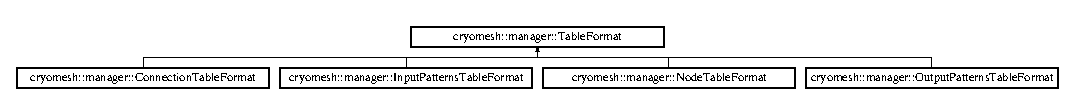
\includegraphics[height=0.968858cm]{structcryomesh_1_1manager_1_1TableFormat}
\end{center}
\end{figure}
\subsection*{\-Public \-Member \-Functions}
\begin{DoxyCompactItemize}
\item 
\hyperlink{structcryomesh_1_1manager_1_1TableFormat_ab19e1f6e34a67772918360f864e40913}{\-Table\-Format} ()
\item 
virtual \hyperlink{structcryomesh_1_1manager_1_1TableFormat_a3dccdd11e7eb1ab2b7720fd8fdc6b019}{$\sim$\-Table\-Format} ()
\item 
std\-::string \hyperlink{structcryomesh_1_1manager_1_1TableFormat_a3e797d6130c6b0745a1fac799c25677a}{get\-Name} () const 
\begin{DoxyCompactList}\small\item\em \-Return the name of the table. \end{DoxyCompactList}\item 
std\-::string \hyperlink{structcryomesh_1_1manager_1_1TableFormat_a2256ce39471582b92bf7cbb6eec74d30}{get\-Key} (const std\-::string \&key)
\begin{DoxyCompactList}\small\item\em \-Return the string object associated with a key. \end{DoxyCompactList}\item 
std\-::string \hyperlink{structcryomesh_1_1manager_1_1TableFormat_a898ae0d0c5490ccdf71aec5156b10fcc}{get\-Create\-Table} () const 
\begin{DoxyCompactList}\small\item\em \-Get the string that can be used to create the sql table. \end{DoxyCompactList}\end{DoxyCompactItemize}
\subsection*{\-Protected \-Attributes}
\begin{DoxyCompactItemize}
\item 
std\-::string \hyperlink{structcryomesh_1_1manager_1_1TableFormat_ab49912897ccb7fd0f8d42f1cc21332e8}{name}
\item 
std\-::map$<$ std\-::string, \*
std\-::string $>$ \hyperlink{structcryomesh_1_1manager_1_1TableFormat_a29ab6f4cfc0c56da1fa461ea665a1b61}{columns}
\end{DoxyCompactItemize}


\subsection{\-Detailed \-Description}
\-General structure of a table. 

\-Definition at line 22 of file \-Table\-Formats.\-h.



\subsection{\-Constructor \& \-Destructor \-Documentation}
\hypertarget{structcryomesh_1_1manager_1_1TableFormat_ab19e1f6e34a67772918360f864e40913}{\index{cryomesh\-::manager\-::\-Table\-Format@{cryomesh\-::manager\-::\-Table\-Format}!\-Table\-Format@{\-Table\-Format}}
\index{\-Table\-Format@{\-Table\-Format}!cryomesh::manager::TableFormat@{cryomesh\-::manager\-::\-Table\-Format}}
\subsubsection[{\-Table\-Format}]{\setlength{\rightskip}{0pt plus 5cm}{\bf cryomesh\-::manager\-::\-Table\-Format\-::\-Table\-Format} (
\begin{DoxyParamCaption}
{}
\end{DoxyParamCaption}
)\hspace{0.3cm}{\ttfamily  \mbox{[}inline\mbox{]}}}}\label{structcryomesh_1_1manager_1_1TableFormat_ab19e1f6e34a67772918360f864e40913}


\-Definition at line 24 of file \-Table\-Formats.\-h.

\hypertarget{structcryomesh_1_1manager_1_1TableFormat_a3dccdd11e7eb1ab2b7720fd8fdc6b019}{\index{cryomesh\-::manager\-::\-Table\-Format@{cryomesh\-::manager\-::\-Table\-Format}!$\sim$\-Table\-Format@{$\sim$\-Table\-Format}}
\index{$\sim$\-Table\-Format@{$\sim$\-Table\-Format}!cryomesh::manager::TableFormat@{cryomesh\-::manager\-::\-Table\-Format}}
\subsubsection[{$\sim$\-Table\-Format}]{\setlength{\rightskip}{0pt plus 5cm}virtual {\bf cryomesh\-::manager\-::\-Table\-Format\-::$\sim$\-Table\-Format} (
\begin{DoxyParamCaption}
{}
\end{DoxyParamCaption}
)\hspace{0.3cm}{\ttfamily  \mbox{[}inline, virtual\mbox{]}}}}\label{structcryomesh_1_1manager_1_1TableFormat_a3dccdd11e7eb1ab2b7720fd8fdc6b019}


\-Definition at line 25 of file \-Table\-Formats.\-h.



\subsection{\-Member \-Function \-Documentation}
\hypertarget{structcryomesh_1_1manager_1_1TableFormat_a898ae0d0c5490ccdf71aec5156b10fcc}{\index{cryomesh\-::manager\-::\-Table\-Format@{cryomesh\-::manager\-::\-Table\-Format}!get\-Create\-Table@{get\-Create\-Table}}
\index{get\-Create\-Table@{get\-Create\-Table}!cryomesh::manager::TableFormat@{cryomesh\-::manager\-::\-Table\-Format}}
\subsubsection[{get\-Create\-Table}]{\setlength{\rightskip}{0pt plus 5cm}std\-::string {\bf cryomesh\-::manager\-::\-Table\-Format\-::get\-Create\-Table} (
\begin{DoxyParamCaption}
{}
\end{DoxyParamCaption}
) const\hspace{0.3cm}{\ttfamily  \mbox{[}inline\mbox{]}}}}\label{structcryomesh_1_1manager_1_1TableFormat_a898ae0d0c5490ccdf71aec5156b10fcc}


\-Get the string that can be used to create the sql table. 

\begin{DoxyReturn}{\-Returns}
the sql command string to create this table 
\end{DoxyReturn}


\-Definition at line 60 of file \-Table\-Formats.\-h.



\-References columns, and get\-Name().

\hypertarget{structcryomesh_1_1manager_1_1TableFormat_a2256ce39471582b92bf7cbb6eec74d30}{\index{cryomesh\-::manager\-::\-Table\-Format@{cryomesh\-::manager\-::\-Table\-Format}!get\-Key@{get\-Key}}
\index{get\-Key@{get\-Key}!cryomesh::manager::TableFormat@{cryomesh\-::manager\-::\-Table\-Format}}
\subsubsection[{get\-Key}]{\setlength{\rightskip}{0pt plus 5cm}std\-::string {\bf cryomesh\-::manager\-::\-Table\-Format\-::get\-Key} (
\begin{DoxyParamCaption}
\item[{const std\-::string \&}]{key}
\end{DoxyParamCaption}
)\hspace{0.3cm}{\ttfamily  \mbox{[}inline\mbox{]}}}}\label{structcryomesh_1_1manager_1_1TableFormat_a2256ce39471582b92bf7cbb6eec74d30}


\-Return the string object associated with a key. 

\-::string \-The key to search for

\begin{DoxyReturn}{\-Returns}
std\-::string \-The object associated with the search key, \char`\"{}\char`\"{} if not found 
\end{DoxyReturn}


\-Definition at line 45 of file \-Table\-Formats.\-h.



\-References columns.

\hypertarget{structcryomesh_1_1manager_1_1TableFormat_a3e797d6130c6b0745a1fac799c25677a}{\index{cryomesh\-::manager\-::\-Table\-Format@{cryomesh\-::manager\-::\-Table\-Format}!get\-Name@{get\-Name}}
\index{get\-Name@{get\-Name}!cryomesh::manager::TableFormat@{cryomesh\-::manager\-::\-Table\-Format}}
\subsubsection[{get\-Name}]{\setlength{\rightskip}{0pt plus 5cm}std\-::string {\bf cryomesh\-::manager\-::\-Table\-Format\-::get\-Name} (
\begin{DoxyParamCaption}
{}
\end{DoxyParamCaption}
) const\hspace{0.3cm}{\ttfamily  \mbox{[}inline\mbox{]}}}}\label{structcryomesh_1_1manager_1_1TableFormat_a3e797d6130c6b0745a1fac799c25677a}


\-Return the name of the table. 

\begin{DoxyReturn}{\-Returns}
std\-::string \-The name of the table 
\end{DoxyReturn}


\-Definition at line 32 of file \-Table\-Formats.\-h.



\-References name.



\-Referenced by get\-Create\-Table(), cryomesh\-::manager\-::\-Database\-Manager\-::insert\-Connection(), cryomesh\-::manager\-::\-Database\-Manager\-::insert\-Node(), and cryomesh\-::manager\-::\-Database\-Manager\-::insert\-Output\-Pattern().



\subsection{\-Member \-Data \-Documentation}
\hypertarget{structcryomesh_1_1manager_1_1TableFormat_a29ab6f4cfc0c56da1fa461ea665a1b61}{\index{cryomesh\-::manager\-::\-Table\-Format@{cryomesh\-::manager\-::\-Table\-Format}!columns@{columns}}
\index{columns@{columns}!cryomesh::manager::TableFormat@{cryomesh\-::manager\-::\-Table\-Format}}
\subsubsection[{columns}]{\setlength{\rightskip}{0pt plus 5cm}std\-::map$<$std\-::string, std\-::string$>$ {\bf cryomesh\-::manager\-::\-Table\-Format\-::columns}\hspace{0.3cm}{\ttfamily  \mbox{[}protected\mbox{]}}}}\label{structcryomesh_1_1manager_1_1TableFormat_a29ab6f4cfc0c56da1fa461ea665a1b61}


\-Definition at line 93 of file \-Table\-Formats.\-h.



\-Referenced by cryomesh\-::manager\-::\-Connection\-Table\-Format\-::\-Connection\-Table\-Format(), get\-Create\-Table(), get\-Key(), cryomesh\-::manager\-::\-Input\-Patterns\-Table\-Format\-::\-Input\-Patterns\-Table\-Format(), cryomesh\-::manager\-::\-Node\-Table\-Format\-::\-Node\-Table\-Format(), and cryomesh\-::manager\-::\-Output\-Patterns\-Table\-Format\-::\-Output\-Patterns\-Table\-Format().

\hypertarget{structcryomesh_1_1manager_1_1TableFormat_ab49912897ccb7fd0f8d42f1cc21332e8}{\index{cryomesh\-::manager\-::\-Table\-Format@{cryomesh\-::manager\-::\-Table\-Format}!name@{name}}
\index{name@{name}!cryomesh::manager::TableFormat@{cryomesh\-::manager\-::\-Table\-Format}}
\subsubsection[{name}]{\setlength{\rightskip}{0pt plus 5cm}std\-::string {\bf cryomesh\-::manager\-::\-Table\-Format\-::name}\hspace{0.3cm}{\ttfamily  \mbox{[}protected\mbox{]}}}}\label{structcryomesh_1_1manager_1_1TableFormat_ab49912897ccb7fd0f8d42f1cc21332e8}


\-Definition at line 86 of file \-Table\-Formats.\-h.



\-Referenced by cryomesh\-::manager\-::\-Connection\-Table\-Format\-::\-Connection\-Table\-Format(), get\-Name(), cryomesh\-::manager\-::\-Input\-Patterns\-Table\-Format\-::\-Input\-Patterns\-Table\-Format(), cryomesh\-::manager\-::\-Node\-Table\-Format\-::\-Node\-Table\-Format(), and cryomesh\-::manager\-::\-Output\-Patterns\-Table\-Format\-::\-Output\-Patterns\-Table\-Format().



\-The documentation for this struct was generated from the following file\-:\begin{DoxyCompactItemize}
\item 
/home/niall/\-Projects/\-Eclipse/\-C\-P\-P/cryomesh/src/manager/\hyperlink{TableFormats_8h}{\-Table\-Formats.\-h}\end{DoxyCompactItemize}

\hypertarget{classcryomesh_1_1common_1_1TimeKeeper}{\section{cryomesh\-:\-:common\-:\-:\-Time\-Keeper \-Class \-Reference}
\label{classcryomesh_1_1common_1_1TimeKeeper}\index{cryomesh\-::common\-::\-Time\-Keeper@{cryomesh\-::common\-::\-Time\-Keeper}}
}


\hyperlink{classcryomesh_1_1common_1_1TimeKeeper}{\-Time\-Keeper} is a class keep track of the cycle state and timing.  




{\ttfamily \#include $<$\-Time\-Keeper.\-h$>$}

\subsection*{\-Public \-Member \-Functions}
\begin{DoxyCompactItemize}
\item 
void \hyperlink{classcryomesh_1_1common_1_1TimeKeeper_abb7b3042e8b2087326c2405a0bc8d230}{reset} ()
\begin{DoxyCompactList}\small\item\em \-Destructor. \end{DoxyCompactList}\item 
virtual \hyperlink{classcryomesh_1_1common_1_1TimeKeeper_a1023707129088652ac2cced3e0f4a0be}{$\sim$\-Time\-Keeper} ()
\item 
bool \hyperlink{classcryomesh_1_1common_1_1TimeKeeper_a7c710ae8bdb2fff0aaf284a9c1108ace}{operator==} (const \hyperlink{classcryomesh_1_1common_1_1TimeKeeper}{\-Time\-Keeper} \&)
\begin{DoxyCompactList}\small\item\em \-Equality test override for object. \end{DoxyCompactList}\item 
void \hyperlink{classcryomesh_1_1common_1_1TimeKeeper_a0581cd24a6eebfbdd67a363467483456}{update} ()
\begin{DoxyCompactList}\small\item\em \-Move the timing on one cycle. \end{DoxyCompactList}\item 
\hyperlink{classcryomesh_1_1common_1_1Cycle}{\-Cycle} \hyperlink{classcryomesh_1_1common_1_1TimeKeeper_aa0bfaecbd5118af91d63296f158cee09}{get\-Cycle} () const 
\begin{DoxyCompactList}\small\item\em \-Get the current cycle we're on as an \hyperlink{classcryomesh_1_1common_1_1Cycle}{\-Cycle}. \end{DoxyCompactList}\item 
std\-::time\-\_\-t \hyperlink{classcryomesh_1_1common_1_1TimeKeeper_a73a685a859e69ce3660b6a6d3469997e}{get\-Start\-Time} () const 
\begin{DoxyCompactList}\small\item\em \-Get the time we started cycling. \end{DoxyCompactList}\item 
double \hyperlink{classcryomesh_1_1common_1_1TimeKeeper_ad3f49c5602d1e51b4ee9aa9535a59454}{get\-Timing} () const 
\begin{DoxyCompactList}\small\item\em \-Difference between the last time and now. \end{DoxyCompactList}\item 
const boost\-::timer \& \hyperlink{classcryomesh_1_1common_1_1TimeKeeper_a888f7db463cc84b0a00478c4bbcf7c44}{get\-Timer} () const 
\begin{DoxyCompactList}\small\item\em \-Get the \-Timer. \end{DoxyCompactList}\end{DoxyCompactItemize}
\subsection*{\-Static \-Public \-Member \-Functions}
\begin{DoxyCompactItemize}
\item 
static \hyperlink{classcryomesh_1_1common_1_1TimeKeeper}{\-Time\-Keeper} \& \hyperlink{classcryomesh_1_1common_1_1TimeKeeper_afe7b229532e11119cb2653192615d679}{get\-Time\-Keeper} ()
\end{DoxyCompactItemize}
\subsection*{\-Protected \-Member \-Functions}
\begin{DoxyCompactItemize}
\item 
\hyperlink{classcryomesh_1_1common_1_1TimeKeeper_a133c730f64b915e6ef25be1442ea688e}{\-Time\-Keeper} ()
\begin{DoxyCompactList}\small\item\em \-Constructor. \end{DoxyCompactList}\item 
\hyperlink{classcryomesh_1_1common_1_1TimeKeeper_a3ea9062a72b2cc0af37b445ed254b64f}{\-Time\-Keeper} (const \hyperlink{classcryomesh_1_1common_1_1TimeKeeper}{\-Time\-Keeper} \&)
\begin{DoxyCompactList}\small\item\em \-Copy \-Constructor. \end{DoxyCompactList}\item 
\hyperlink{classcryomesh_1_1common_1_1TimeKeeper}{\-Time\-Keeper} \& \hyperlink{classcryomesh_1_1common_1_1TimeKeeper_ad22e5329268d4e6f55b4a29045c11035}{operator=} (const \hyperlink{classcryomesh_1_1common_1_1TimeKeeper}{\-Time\-Keeper} \&)
\begin{DoxyCompactList}\small\item\em \-Assignment \-Operator. \end{DoxyCompactList}\end{DoxyCompactItemize}
\subsection*{\-Private \-Attributes}
\begin{DoxyCompactItemize}
\item 
\hyperlink{classcryomesh_1_1common_1_1Cycle}{\-Cycle} \hyperlink{classcryomesh_1_1common_1_1TimeKeeper_af2f511fb5df5b4a1e6d9eb8dffa4f6ef}{cycle}
\item 
std\-::time\-\_\-t \hyperlink{classcryomesh_1_1common_1_1TimeKeeper_ad6e92ec3c962aa3e6db82d69188e9686}{start\-\_\-time}
\item 
boost\-::timer \hyperlink{classcryomesh_1_1common_1_1TimeKeeper_a41690fc156fdee825fb5e7a5e26a2102}{timer}
\item 
double \hyperlink{classcryomesh_1_1common_1_1TimeKeeper_afe9c0b2cd669e9d4d62718734e5b630a}{this\-\_\-timing}
\item 
double \hyperlink{classcryomesh_1_1common_1_1TimeKeeper_acb896ec81cbe9d18f4e618320353dc4f}{last\-\_\-timing}
\end{DoxyCompactItemize}
\subsection*{\-Static \-Private \-Attributes}
\begin{DoxyCompactItemize}
\item 
static boost\-::shared\-\_\-ptr\*
$<$ \hyperlink{classcryomesh_1_1common_1_1TimeKeeper}{\-Time\-Keeper} $>$ \hyperlink{classcryomesh_1_1common_1_1TimeKeeper_a9182b02e3805961510f48954276ef389}{timekeeper}
\end{DoxyCompactItemize}


\subsection{\-Detailed \-Description}
\hyperlink{classcryomesh_1_1common_1_1TimeKeeper}{\-Time\-Keeper} is a class keep track of the cycle state and timing. 

\hyperlink{classcryomesh_1_1common_1_1TimeKeeper}{\-Time\-Keeper} manages the 'tick' cycle and provides the means by which classes throughout the system can keep track of the cycle 

\-Definition at line 31 of file \-Time\-Keeper.\-h.



\subsection{\-Constructor \& \-Destructor \-Documentation}
\hypertarget{classcryomesh_1_1common_1_1TimeKeeper_a1023707129088652ac2cced3e0f4a0be}{\index{cryomesh\-::common\-::\-Time\-Keeper@{cryomesh\-::common\-::\-Time\-Keeper}!$\sim$\-Time\-Keeper@{$\sim$\-Time\-Keeper}}
\index{$\sim$\-Time\-Keeper@{$\sim$\-Time\-Keeper}!cryomesh::common::TimeKeeper@{cryomesh\-::common\-::\-Time\-Keeper}}
\subsubsection[{$\sim$\-Time\-Keeper}]{\setlength{\rightskip}{0pt plus 5cm}{\bf cryomesh\-::common\-::\-Time\-Keeper\-::$\sim$\-Time\-Keeper} (
\begin{DoxyParamCaption}
{}
\end{DoxyParamCaption}
)\hspace{0.3cm}{\ttfamily  \mbox{[}virtual\mbox{]}}}}\label{classcryomesh_1_1common_1_1TimeKeeper_a1023707129088652ac2cced3e0f4a0be}


\-Definition at line 37 of file \-Time\-Keeper.\-cpp.

\hypertarget{classcryomesh_1_1common_1_1TimeKeeper_a133c730f64b915e6ef25be1442ea688e}{\index{cryomesh\-::common\-::\-Time\-Keeper@{cryomesh\-::common\-::\-Time\-Keeper}!\-Time\-Keeper@{\-Time\-Keeper}}
\index{\-Time\-Keeper@{\-Time\-Keeper}!cryomesh::common::TimeKeeper@{cryomesh\-::common\-::\-Time\-Keeper}}
\subsubsection[{\-Time\-Keeper}]{\setlength{\rightskip}{0pt plus 5cm}{\bf cryomesh\-::common\-::\-Time\-Keeper\-::\-Time\-Keeper} (
\begin{DoxyParamCaption}
{}
\end{DoxyParamCaption}
)\hspace{0.3cm}{\ttfamily  \mbox{[}protected\mbox{]}}}}\label{classcryomesh_1_1common_1_1TimeKeeper_a133c730f64b915e6ef25be1442ea688e}


\-Constructor. 

\-Constructor for \hyperlink{classcryomesh_1_1common_1_1TimeKeeper}{\-Time\-Keeper}. \-Inaccessible to force singleton class 

\-Definition at line 34 of file \-Time\-Keeper.\-cpp.



\-References reset().



\-Referenced by get\-Time\-Keeper().

\hypertarget{classcryomesh_1_1common_1_1TimeKeeper_a3ea9062a72b2cc0af37b445ed254b64f}{\index{cryomesh\-::common\-::\-Time\-Keeper@{cryomesh\-::common\-::\-Time\-Keeper}!\-Time\-Keeper@{\-Time\-Keeper}}
\index{\-Time\-Keeper@{\-Time\-Keeper}!cryomesh::common::TimeKeeper@{cryomesh\-::common\-::\-Time\-Keeper}}
\subsubsection[{\-Time\-Keeper}]{\setlength{\rightskip}{0pt plus 5cm}{\bf cryomesh\-::common\-::\-Time\-Keeper\-::\-Time\-Keeper} (
\begin{DoxyParamCaption}
\item[{const {\bf \-Time\-Keeper} \&}]{}
\end{DoxyParamCaption}
)\hspace{0.3cm}{\ttfamily  \mbox{[}protected\mbox{]}}}}\label{classcryomesh_1_1common_1_1TimeKeeper_a3ea9062a72b2cc0af37b445ed254b64f}


\-Copy \-Constructor. 

\-Overridden \-Copy \-Contructor for \hyperlink{classcryomesh_1_1common_1_1TimeKeeper}{\-Time\-Keeper}. \-Inaccessible to force singleton class


\begin{DoxyParams}{\-Parameters}
{\em \hyperlink{classcryomesh_1_1common_1_1TimeKeeper}{\-Time\-Keeper}} & \-Object to \-Copy \-Construct from \\
\hline
\end{DoxyParams}


\subsection{\-Member \-Function \-Documentation}
\hypertarget{classcryomesh_1_1common_1_1TimeKeeper_aa0bfaecbd5118af91d63296f158cee09}{\index{cryomesh\-::common\-::\-Time\-Keeper@{cryomesh\-::common\-::\-Time\-Keeper}!get\-Cycle@{get\-Cycle}}
\index{get\-Cycle@{get\-Cycle}!cryomesh::common::TimeKeeper@{cryomesh\-::common\-::\-Time\-Keeper}}
\subsubsection[{get\-Cycle}]{\setlength{\rightskip}{0pt plus 5cm}{\bf \-Cycle} {\bf cryomesh\-::common\-::\-Time\-Keeper\-::get\-Cycle} (
\begin{DoxyParamCaption}
{}
\end{DoxyParamCaption}
) const}}\label{classcryomesh_1_1common_1_1TimeKeeper_aa0bfaecbd5118af91d63296f158cee09}


\-Get the current cycle we're on as an \hyperlink{classcryomesh_1_1common_1_1Cycle}{\-Cycle}. 

\begin{DoxyReturn}{\-Returns}
\hyperlink{classcryomesh_1_1common_1_1Cycle}{\-Cycle} \-The cycle we're currently on 
\end{DoxyReturn}


\-Definition at line 76 of file \-Time\-Keeper.\-cpp.



\-References cycle.



\-Referenced by cryomesh\-::manager\-::\-Database\-Manager\-::add\-History\-Entry(), cryomesh\-::components\-::\-Impulse\-Collection\-::clear\-Active\-Impulses(), cryomesh\-::components\-::\-Impulse\-Collection\-::clear\-Impulses(), cryomesh\-::components\-::\-Impulse\-Collection\-::get\-Activity(), cryomesh\-::state\-::\-Pattern\-::get\-Database\-Object(), cryomesh\-::components\-::\-Connection\-::get\-Database\-Object(), cryomesh\-::components\-::\-Node\-::get\-Database\-Object(), cryomesh\-::state\-::\-Pattern\-Channel\-::get\-Pattern\-By\-Cycle(), cryomesh\-::utilities\-::operator$<$$<$(), cryomesh\-::structures\-::\-Bundle\-::print(), cryomesh\-::manager\-::\-Database\-Manager\-::print\-History(), and cryomesh\-::components\-::\-Impulse\-Collection\-::refresh\-Data\-Object().

\hypertarget{classcryomesh_1_1common_1_1TimeKeeper_a73a685a859e69ce3660b6a6d3469997e}{\index{cryomesh\-::common\-::\-Time\-Keeper@{cryomesh\-::common\-::\-Time\-Keeper}!get\-Start\-Time@{get\-Start\-Time}}
\index{get\-Start\-Time@{get\-Start\-Time}!cryomesh::common::TimeKeeper@{cryomesh\-::common\-::\-Time\-Keeper}}
\subsubsection[{get\-Start\-Time}]{\setlength{\rightskip}{0pt plus 5cm}std\-::time\-\_\-t {\bf cryomesh\-::common\-::\-Time\-Keeper\-::get\-Start\-Time} (
\begin{DoxyParamCaption}
{}
\end{DoxyParamCaption}
) const}}\label{classcryomesh_1_1common_1_1TimeKeeper_a73a685a859e69ce3660b6a6d3469997e}


\-Get the time we started cycling. 

\begin{DoxyReturn}{\-Returns}
time\-\_\-t \-The start time 
\end{DoxyReturn}


\-Definition at line 83 of file \-Time\-Keeper.\-cpp.



\-References start\-\_\-time.

\hypertarget{classcryomesh_1_1common_1_1TimeKeeper_afe7b229532e11119cb2653192615d679}{\index{cryomesh\-::common\-::\-Time\-Keeper@{cryomesh\-::common\-::\-Time\-Keeper}!get\-Time\-Keeper@{get\-Time\-Keeper}}
\index{get\-Time\-Keeper@{get\-Time\-Keeper}!cryomesh::common::TimeKeeper@{cryomesh\-::common\-::\-Time\-Keeper}}
\subsubsection[{get\-Time\-Keeper}]{\setlength{\rightskip}{0pt plus 5cm}{\bf \-Time\-Keeper} \& {\bf cryomesh\-::common\-::\-Time\-Keeper\-::get\-Time\-Keeper} (
\begin{DoxyParamCaption}
{}
\end{DoxyParamCaption}
)\hspace{0.3cm}{\ttfamily  \mbox{[}static\mbox{]}}}}\label{classcryomesh_1_1common_1_1TimeKeeper_afe7b229532e11119cb2653192615d679}


\-Definition at line 19 of file \-Time\-Keeper.\-cpp.



\-References \-Time\-Keeper(), and timekeeper.



\-Referenced by cryomesh\-::manager\-::\-Database\-Manager\-::add\-History\-Entry(), cryomesh\-::components\-::\-Node\-::add\-Impulse(), cryomesh\-::components\-::\-Impulse\-Collection\-::clear\-Active\-Impulses(), cryomesh\-::components\-::\-Impulse\-Collection\-::clear\-Impulses(), cryomesh\-::components\-::\-Node\-::enter\-Recovery(), cryomesh\-::components\-::\-Impulse\-Collection\-::get\-Activity(), cryomesh\-::components\-::\-Impulse\-::get\-Activity(), cryomesh\-::components\-::\-Node\-::get\-Activity(), cryomesh\-::components\-::\-Connection\-Map\-::get\-Activity\-Pattern(), cryomesh\-::state\-::\-Pattern\-::get\-Database\-Object(), cryomesh\-::components\-::\-Connection\-::get\-Database\-Object(), cryomesh\-::components\-::\-Node\-::get\-Database\-Object(), cryomesh\-::state\-::\-Pattern\-Channel\-::get\-Pattern\-By\-Cycle(), cryomesh\-::components\-::\-Impulse\-::is\-Active(), cryomesh\-::utilities\-::operator$<$$<$(), cryomesh\-::structures\-::\-Bundle\-::print(), cryomesh\-::manager\-::\-Database\-Manager\-::print\-History(), cryomesh\-::components\-::\-Impulse\-Collection\-::refresh\-Data\-Object(), cryomesh\-::components\-::\-Node\-::set\-Activity(), and cryomesh\-::structures\-::\-Bundle\-::update().

\hypertarget{classcryomesh_1_1common_1_1TimeKeeper_a888f7db463cc84b0a00478c4bbcf7c44}{\index{cryomesh\-::common\-::\-Time\-Keeper@{cryomesh\-::common\-::\-Time\-Keeper}!get\-Timer@{get\-Timer}}
\index{get\-Timer@{get\-Timer}!cryomesh::common::TimeKeeper@{cryomesh\-::common\-::\-Time\-Keeper}}
\subsubsection[{get\-Timer}]{\setlength{\rightskip}{0pt plus 5cm}const boost\-::timer \& {\bf cryomesh\-::common\-::\-Time\-Keeper\-::get\-Timer} (
\begin{DoxyParamCaption}
{}
\end{DoxyParamCaption}
) const}}\label{classcryomesh_1_1common_1_1TimeKeeper_a888f7db463cc84b0a00478c4bbcf7c44}


\-Get the \-Timer. 

\begin{DoxyReturn}{\-Returns}
boost\-::\-Timer 
\end{DoxyReturn}


\-Definition at line 87 of file \-Time\-Keeper.\-cpp.



\-References timer.

\hypertarget{classcryomesh_1_1common_1_1TimeKeeper_ad3f49c5602d1e51b4ee9aa9535a59454}{\index{cryomesh\-::common\-::\-Time\-Keeper@{cryomesh\-::common\-::\-Time\-Keeper}!get\-Timing@{get\-Timing}}
\index{get\-Timing@{get\-Timing}!cryomesh::common::TimeKeeper@{cryomesh\-::common\-::\-Time\-Keeper}}
\subsubsection[{get\-Timing}]{\setlength{\rightskip}{0pt plus 5cm}double {\bf cryomesh\-::common\-::\-Time\-Keeper\-::get\-Timing} (
\begin{DoxyParamCaption}
{}
\end{DoxyParamCaption}
) const}}\label{classcryomesh_1_1common_1_1TimeKeeper_ad3f49c5602d1e51b4ee9aa9535a59454}


\-Difference between the last time and now. 

\begin{DoxyReturn}{\-Returns}
double \-The difference between the clock now and the last clock 
\end{DoxyReturn}


\-Definition at line 80 of file \-Time\-Keeper.\-cpp.



\-References last\-\_\-timing, and this\-\_\-timing.

\hypertarget{classcryomesh_1_1common_1_1TimeKeeper_ad22e5329268d4e6f55b4a29045c11035}{\index{cryomesh\-::common\-::\-Time\-Keeper@{cryomesh\-::common\-::\-Time\-Keeper}!operator=@{operator=}}
\index{operator=@{operator=}!cryomesh::common::TimeKeeper@{cryomesh\-::common\-::\-Time\-Keeper}}
\subsubsection[{operator=}]{\setlength{\rightskip}{0pt plus 5cm}{\bf \-Time\-Keeper}\& cryomesh\-::common\-::\-Time\-Keeper\-::operator= (
\begin{DoxyParamCaption}
\item[{const {\bf \-Time\-Keeper} \&}]{}
\end{DoxyParamCaption}
)\hspace{0.3cm}{\ttfamily  \mbox{[}protected\mbox{]}}}}\label{classcryomesh_1_1common_1_1TimeKeeper_ad22e5329268d4e6f55b4a29045c11035}


\-Assignment \-Operator. 

\-Overridden \-Assignment \-Operator for \hyperlink{classcryomesh_1_1common_1_1TimeKeeper}{\-Time\-Keeper}. \-Inaccessible to force singleton class


\begin{DoxyParams}{\-Parameters}
{\em \hyperlink{classcryomesh_1_1common_1_1TimeKeeper}{\-Time\-Keeper}} & \-Object to \-Assign this to \\
\hline
\end{DoxyParams}
\hypertarget{classcryomesh_1_1common_1_1TimeKeeper_a7c710ae8bdb2fff0aaf284a9c1108ace}{\index{cryomesh\-::common\-::\-Time\-Keeper@{cryomesh\-::common\-::\-Time\-Keeper}!operator==@{operator==}}
\index{operator==@{operator==}!cryomesh::common::TimeKeeper@{cryomesh\-::common\-::\-Time\-Keeper}}
\subsubsection[{operator==}]{\setlength{\rightskip}{0pt plus 5cm}bool cryomesh\-::common\-::\-Time\-Keeper\-::operator== (
\begin{DoxyParamCaption}
\item[{const {\bf \-Time\-Keeper} \&}]{obj}
\end{DoxyParamCaption}
)}}\label{classcryomesh_1_1common_1_1TimeKeeper_a7c710ae8bdb2fff0aaf284a9c1108ace}


\-Equality test override for object. 


\begin{DoxyParams}{\-Parameters}
{\em \hyperlink{classcryomesh_1_1common_1_1TimeKeeper}{\-Time\-Keeper}} & obj \-Object to compare this with\\
\hline
\end{DoxyParams}
\begin{DoxyReturn}{\-Returns}
bool \-True if equal, false otherwise 
\end{DoxyReturn}


\-Definition at line 40 of file \-Time\-Keeper.\-cpp.



\-References cycle, last\-\_\-timing, start\-\_\-time, and this\-\_\-timing.

\hypertarget{classcryomesh_1_1common_1_1TimeKeeper_abb7b3042e8b2087326c2405a0bc8d230}{\index{cryomesh\-::common\-::\-Time\-Keeper@{cryomesh\-::common\-::\-Time\-Keeper}!reset@{reset}}
\index{reset@{reset}!cryomesh::common::TimeKeeper@{cryomesh\-::common\-::\-Time\-Keeper}}
\subsubsection[{reset}]{\setlength{\rightskip}{0pt plus 5cm}void {\bf cryomesh\-::common\-::\-Time\-Keeper\-::reset} (
\begin{DoxyParamCaption}
{}
\end{DoxyParamCaption}
)}}\label{classcryomesh_1_1common_1_1TimeKeeper_abb7b3042e8b2087326c2405a0bc8d230}


\-Destructor. 

\-Destructor for \hyperlink{classcryomesh_1_1common_1_1TimeKeeper}{\-Time\-Keeper} \-Reset the timekeeper 

\-Definition at line 26 of file \-Time\-Keeper.\-cpp.



\-References cycle, last\-\_\-timing, start\-\_\-time, this\-\_\-timing, and timer.



\-Referenced by \-Time\-Keeper().

\hypertarget{classcryomesh_1_1common_1_1TimeKeeper_a0581cd24a6eebfbdd67a363467483456}{\index{cryomesh\-::common\-::\-Time\-Keeper@{cryomesh\-::common\-::\-Time\-Keeper}!update@{update}}
\index{update@{update}!cryomesh::common::TimeKeeper@{cryomesh\-::common\-::\-Time\-Keeper}}
\subsubsection[{update}]{\setlength{\rightskip}{0pt plus 5cm}void {\bf cryomesh\-::common\-::\-Time\-Keeper\-::update} (
\begin{DoxyParamCaption}
{}
\end{DoxyParamCaption}
)}}\label{classcryomesh_1_1common_1_1TimeKeeper_a0581cd24a6eebfbdd67a363467483456}


\-Move the timing on one cycle. 



\-Definition at line 66 of file \-Time\-Keeper.\-cpp.



\-References cycle, last\-\_\-timing, this\-\_\-timing, and timer.



\-Referenced by cryomesh\-::structures\-::\-Bundle\-::update().



\subsection{\-Member \-Data \-Documentation}
\hypertarget{classcryomesh_1_1common_1_1TimeKeeper_af2f511fb5df5b4a1e6d9eb8dffa4f6ef}{\index{cryomesh\-::common\-::\-Time\-Keeper@{cryomesh\-::common\-::\-Time\-Keeper}!cycle@{cycle}}
\index{cycle@{cycle}!cryomesh::common::TimeKeeper@{cryomesh\-::common\-::\-Time\-Keeper}}
\subsubsection[{cycle}]{\setlength{\rightskip}{0pt plus 5cm}{\bf \-Cycle} {\bf cryomesh\-::common\-::\-Time\-Keeper\-::cycle}\hspace{0.3cm}{\ttfamily  \mbox{[}private\mbox{]}}}}\label{classcryomesh_1_1common_1_1TimeKeeper_af2f511fb5df5b4a1e6d9eb8dffa4f6ef}


\-Definition at line 159 of file \-Time\-Keeper.\-h.



\-Referenced by get\-Cycle(), operator==(), reset(), and update().

\hypertarget{classcryomesh_1_1common_1_1TimeKeeper_acb896ec81cbe9d18f4e618320353dc4f}{\index{cryomesh\-::common\-::\-Time\-Keeper@{cryomesh\-::common\-::\-Time\-Keeper}!last\-\_\-timing@{last\-\_\-timing}}
\index{last\-\_\-timing@{last\-\_\-timing}!cryomesh::common::TimeKeeper@{cryomesh\-::common\-::\-Time\-Keeper}}
\subsubsection[{last\-\_\-timing}]{\setlength{\rightskip}{0pt plus 5cm}double {\bf cryomesh\-::common\-::\-Time\-Keeper\-::last\-\_\-timing}\hspace{0.3cm}{\ttfamily  \mbox{[}private\mbox{]}}}}\label{classcryomesh_1_1common_1_1TimeKeeper_acb896ec81cbe9d18f4e618320353dc4f}


\-Definition at line 187 of file \-Time\-Keeper.\-h.



\-Referenced by get\-Timing(), operator==(), reset(), and update().

\hypertarget{classcryomesh_1_1common_1_1TimeKeeper_ad6e92ec3c962aa3e6db82d69188e9686}{\index{cryomesh\-::common\-::\-Time\-Keeper@{cryomesh\-::common\-::\-Time\-Keeper}!start\-\_\-time@{start\-\_\-time}}
\index{start\-\_\-time@{start\-\_\-time}!cryomesh::common::TimeKeeper@{cryomesh\-::common\-::\-Time\-Keeper}}
\subsubsection[{start\-\_\-time}]{\setlength{\rightskip}{0pt plus 5cm}std\-::time\-\_\-t {\bf cryomesh\-::common\-::\-Time\-Keeper\-::start\-\_\-time}\hspace{0.3cm}{\ttfamily  \mbox{[}private\mbox{]}}}}\label{classcryomesh_1_1common_1_1TimeKeeper_ad6e92ec3c962aa3e6db82d69188e9686}


\-Definition at line 166 of file \-Time\-Keeper.\-h.



\-Referenced by get\-Start\-Time(), operator==(), and reset().

\hypertarget{classcryomesh_1_1common_1_1TimeKeeper_afe9c0b2cd669e9d4d62718734e5b630a}{\index{cryomesh\-::common\-::\-Time\-Keeper@{cryomesh\-::common\-::\-Time\-Keeper}!this\-\_\-timing@{this\-\_\-timing}}
\index{this\-\_\-timing@{this\-\_\-timing}!cryomesh::common::TimeKeeper@{cryomesh\-::common\-::\-Time\-Keeper}}
\subsubsection[{this\-\_\-timing}]{\setlength{\rightskip}{0pt plus 5cm}double {\bf cryomesh\-::common\-::\-Time\-Keeper\-::this\-\_\-timing}\hspace{0.3cm}{\ttfamily  \mbox{[}private\mbox{]}}}}\label{classcryomesh_1_1common_1_1TimeKeeper_afe9c0b2cd669e9d4d62718734e5b630a}


\-Definition at line 180 of file \-Time\-Keeper.\-h.



\-Referenced by get\-Timing(), operator==(), reset(), and update().

\hypertarget{classcryomesh_1_1common_1_1TimeKeeper_a9182b02e3805961510f48954276ef389}{\index{cryomesh\-::common\-::\-Time\-Keeper@{cryomesh\-::common\-::\-Time\-Keeper}!timekeeper@{timekeeper}}
\index{timekeeper@{timekeeper}!cryomesh::common::TimeKeeper@{cryomesh\-::common\-::\-Time\-Keeper}}
\subsubsection[{timekeeper}]{\setlength{\rightskip}{0pt plus 5cm}boost\-::shared\-\_\-ptr$<$ {\bf \-Time\-Keeper} $>$ {\bf cryomesh\-::common\-::\-Time\-Keeper\-::timekeeper}\hspace{0.3cm}{\ttfamily  \mbox{[}static, private\mbox{]}}}}\label{classcryomesh_1_1common_1_1TimeKeeper_a9182b02e3805961510f48954276ef389}


\-Definition at line 151 of file \-Time\-Keeper.\-h.



\-Referenced by get\-Time\-Keeper().

\hypertarget{classcryomesh_1_1common_1_1TimeKeeper_a41690fc156fdee825fb5e7a5e26a2102}{\index{cryomesh\-::common\-::\-Time\-Keeper@{cryomesh\-::common\-::\-Time\-Keeper}!timer@{timer}}
\index{timer@{timer}!cryomesh::common::TimeKeeper@{cryomesh\-::common\-::\-Time\-Keeper}}
\subsubsection[{timer}]{\setlength{\rightskip}{0pt plus 5cm}boost\-::timer {\bf cryomesh\-::common\-::\-Time\-Keeper\-::timer}\hspace{0.3cm}{\ttfamily  \mbox{[}private\mbox{]}}}}\label{classcryomesh_1_1common_1_1TimeKeeper_a41690fc156fdee825fb5e7a5e26a2102}


\-Definition at line 173 of file \-Time\-Keeper.\-h.



\-Referenced by get\-Timer(), reset(), and update().



\-The documentation for this class was generated from the following files\-:\begin{DoxyCompactItemize}
\item 
/home/niall/\-Projects/\-Eclipse/\-C\-P\-P/cryomesh/src/common/\hyperlink{TimeKeeper_8h}{\-Time\-Keeper.\-h}\item 
/home/niall/\-Projects/\-Eclipse/\-C\-P\-P/cryomesh/src/common/\hyperlink{TimeKeeper_8cpp}{\-Time\-Keeper.\-cpp}\end{DoxyCompactItemize}

\chapter{\-File \-Documentation}
\hypertarget{Connector_8h}{\section{/home/niall/\-Projects/\-Eclipse/\-C\-P\-P/cryomesh/src/common/\-Connector.h \-File \-Reference}
\label{Connector_8h}\index{/home/niall/\-Projects/\-Eclipse/\-C\-P\-P/cryomesh/src/common/\-Connector.\-h@{/home/niall/\-Projects/\-Eclipse/\-C\-P\-P/cryomesh/src/common/\-Connector.\-h}}
}
{\ttfamily \#include \char`\"{}common/\-Cycle.\-h\char`\"{}}\*
{\ttfamily \#include $<$map$>$}\*
{\ttfamily \#include $<$boost/shared\-\_\-ptr.\-hpp$>$}\*
{\ttfamily \#include $<$boost/uuid/uuid.\-hpp$>$}\*
{\ttfamily \#include $<$boost/uuid/uuid\-\_\-io.\-hpp$>$}\*
{\ttfamily \#include \char`\"{}common/\-Misc.\-h\char`\"{}}\*
\subsection*{\-Classes}
\begin{DoxyCompactItemize}
\item 
class \hyperlink{classcryomesh_1_1common_1_1Connector}{cryomesh\-::common\-::\-Connector$<$ U, T $>$}
\begin{DoxyCompactList}\small\item\em \hyperlink{classcryomesh_1_1common_1_1Connector}{\-Connector} is a template to add connectable functionality between two classes. \end{DoxyCompactList}\end{DoxyCompactItemize}
\subsection*{\-Namespaces}
\begin{DoxyCompactItemize}
\item 
namespace \hyperlink{namespacecryomesh}{cryomesh}
\begin{DoxyCompactList}\small\item\em \hyperlink{Connector_8h}{\-Connector.\-h}. \end{DoxyCompactList}\item 
namespace \hyperlink{namespacecryomesh_1_1common}{cryomesh\-::common}
\end{DoxyCompactItemize}

\hypertarget{Cycle_8cpp}{\section{/home/niall/\-Projects/\-Eclipse/\-C\-P\-P/cryomesh/src/common/\-Cycle.cpp \-File \-Reference}
\label{Cycle_8cpp}\index{/home/niall/\-Projects/\-Eclipse/\-C\-P\-P/cryomesh/src/common/\-Cycle.\-cpp@{/home/niall/\-Projects/\-Eclipse/\-C\-P\-P/cryomesh/src/common/\-Cycle.\-cpp}}
}
{\ttfamily \#include \char`\"{}\-Cycle.\-h\char`\"{}}\*
{\ttfamily \#include $<$iostream$>$}\*
\subsection*{\-Namespaces}
\begin{DoxyCompactItemize}
\item 
namespace \hyperlink{namespacecryomesh}{cryomesh}
\begin{DoxyCompactList}\small\item\em \hyperlink{Connector_8h}{\-Connector.\-h}. \end{DoxyCompactList}\item 
namespace \hyperlink{namespacecryomesh_1_1common}{cryomesh\-::common}
\end{DoxyCompactItemize}
\subsection*{\-Functions}
\begin{DoxyCompactItemize}
\item 
std\-::ostream \& \hyperlink{namespacecryomesh_1_1common_a09ffb633342203192e93c454f4dbd6f9}{cryomesh\-::common\-::operator$<$$<$} (std\-::ostream \&os, const \-Cycle \&obj)
\end{DoxyCompactItemize}

\hypertarget{Cycle_8h}{\section{/home/niall/\-Projects/\-Eclipse/\-C\-P\-P/cryomesh/src/common/\-Cycle.h \-File \-Reference}
\label{Cycle_8h}\index{/home/niall/\-Projects/\-Eclipse/\-C\-P\-P/cryomesh/src/common/\-Cycle.\-h@{/home/niall/\-Projects/\-Eclipse/\-C\-P\-P/cryomesh/src/common/\-Cycle.\-h}}
}
{\ttfamily \#include $<$gmpxx.\-h$>$}\*
\subsection*{\-Classes}
\begin{DoxyCompactItemize}
\item 
class \hyperlink{classcryomesh_1_1common_1_1Cycle}{cryomesh\-::common\-::\-Cycle}
\end{DoxyCompactItemize}
\subsection*{\-Namespaces}
\begin{DoxyCompactItemize}
\item 
namespace \hyperlink{namespacecryomesh}{cryomesh}
\begin{DoxyCompactList}\small\item\em \hyperlink{Connector_8h}{\-Connector.\-h}. \end{DoxyCompactList}\item 
namespace \hyperlink{namespacecryomesh_1_1common}{cryomesh\-::common}
\end{DoxyCompactItemize}

\hypertarget{Loggable_8h}{\section{/home/niall/\-Projects/\-Eclipse/\-C\-P\-P/cryomesh/src/common/\-Loggable.h \-File \-Reference}
\label{Loggable_8h}\index{/home/niall/\-Projects/\-Eclipse/\-C\-P\-P/cryomesh/src/common/\-Loggable.\-h@{/home/niall/\-Projects/\-Eclipse/\-C\-P\-P/cryomesh/src/common/\-Loggable.\-h}}
}
{\ttfamily \#include $<$iostream$>$}\*
\subsection*{\-Classes}
\begin{DoxyCompactItemize}
\item 
class \hyperlink{classcryomesh_1_1common_1_1Loggable}{cryomesh\-::common\-::\-Loggable}
\end{DoxyCompactItemize}
\subsection*{\-Namespaces}
\begin{DoxyCompactItemize}
\item 
namespace \hyperlink{namespacecryomesh}{cryomesh}
\begin{DoxyCompactList}\small\item\em \hyperlink{Connector_8h}{\-Connector.\-h}. \end{DoxyCompactList}\item 
namespace \hyperlink{namespacecryomesh_1_1common}{cryomesh\-::common}
\end{DoxyCompactItemize}

\hypertarget{TimeKeeper_8cpp}{\section{/home/niall/\-Projects/\-Eclipse/\-C\-P\-P/cryomesh/src/common/\-Time\-Keeper.cpp \-File \-Reference}
\label{TimeKeeper_8cpp}\index{/home/niall/\-Projects/\-Eclipse/\-C\-P\-P/cryomesh/src/common/\-Time\-Keeper.\-cpp@{/home/niall/\-Projects/\-Eclipse/\-C\-P\-P/cryomesh/src/common/\-Time\-Keeper.\-cpp}}
}
{\ttfamily \#include \char`\"{}\-Time\-Keeper.\-h\char`\"{}}\*
{\ttfamily \#include $<$iostream$>$}\*
{\ttfamily \#include $<$ctime$>$}\*
{\ttfamily \#include $<$time.\-h$>$}\*
\subsection*{\-Namespaces}
\begin{DoxyCompactItemize}
\item 
namespace \hyperlink{namespacecryomesh}{cryomesh}
\begin{DoxyCompactList}\small\item\em \hyperlink{Connector_8h}{\-Connector.\-h}. \end{DoxyCompactList}\item 
namespace \hyperlink{namespacecryomesh_1_1common}{cryomesh\-::common}
\end{DoxyCompactItemize}

\hypertarget{TimeKeeper_8h}{\section{/home/niall/\-Projects/\-Eclipse/\-C\-P\-P/cryomesh/src/common/\-Time\-Keeper.h \-File \-Reference}
\label{TimeKeeper_8h}\index{/home/niall/\-Projects/\-Eclipse/\-C\-P\-P/cryomesh/src/common/\-Time\-Keeper.\-h@{/home/niall/\-Projects/\-Eclipse/\-C\-P\-P/cryomesh/src/common/\-Time\-Keeper.\-h}}
}
{\ttfamily \#include \char`\"{}common/\-Cycle.\-h\char`\"{}}\*
{\ttfamily \#include $<$boost/shared\-\_\-ptr.\-hpp$>$}\*
{\ttfamily \#include $<$boost/serialization/shared\-\_\-ptr.\-hpp$>$}\*
{\ttfamily \#include $<$boost/date\-\_\-time/posix\-\_\-time/posix\-\_\-time.\-hpp$>$}\*
{\ttfamily \#include $<$boost/timer.\-hpp$>$}\*
{\ttfamily \#include $<$time.\-h$>$}\*
\subsection*{\-Classes}
\begin{DoxyCompactItemize}
\item 
class \hyperlink{classcryomesh_1_1common_1_1TimeKeeper}{cryomesh\-::common\-::\-Time\-Keeper}
\begin{DoxyCompactList}\small\item\em \hyperlink{classcryomesh_1_1common_1_1TimeKeeper}{\-Time\-Keeper} is a class keep track of the cycle state and timing. \end{DoxyCompactList}\end{DoxyCompactItemize}
\subsection*{\-Namespaces}
\begin{DoxyCompactItemize}
\item 
namespace \hyperlink{namespacecryomesh}{cryomesh}
\begin{DoxyCompactList}\small\item\em \hyperlink{Connector_8h}{\-Connector.\-h}. \end{DoxyCompactList}\item 
namespace \hyperlink{namespacecryomesh_1_1common}{cryomesh\-::common}
\end{DoxyCompactItemize}

\hypertarget{ActivityTimer_8h}{\section{/home/niall/\-Projects/\-Eclipse/\-C\-P\-P/cryomesh/src/components/\-Activity\-Timer.h \-File \-Reference}
\label{ActivityTimer_8h}\index{/home/niall/\-Projects/\-Eclipse/\-C\-P\-P/cryomesh/src/components/\-Activity\-Timer.\-h@{/home/niall/\-Projects/\-Eclipse/\-C\-P\-P/cryomesh/src/components/\-Activity\-Timer.\-h}}
}
{\ttfamily \#include $<$ostream$>$}\*
\subsection*{\-Classes}
\begin{DoxyCompactItemize}
\item 
class \hyperlink{classcryomesh_1_1components_1_1ActivityTimer}{cryomesh\-::components\-::\-Activity\-Timer}
\begin{DoxyCompactList}\small\item\em \-Simple interface class for activity timers. \end{DoxyCompactList}\end{DoxyCompactItemize}
\subsection*{\-Namespaces}
\begin{DoxyCompactItemize}
\item 
namespace \hyperlink{namespacecryomesh}{cryomesh}
\begin{DoxyCompactList}\small\item\em \hyperlink{Connector_8h}{\-Connector.\-h}. \end{DoxyCompactList}\item 
namespace \hyperlink{namespacecryomesh_1_1components}{cryomesh\-::components}
\end{DoxyCompactItemize}

\hypertarget{ActivityTimerDistance_8cpp}{\section{/home/niall/\-Projects/\-Eclipse/\-C\-P\-P/cryomesh/src/components/\-Activity\-Timer\-Distance.cpp \-File \-Reference}
\label{ActivityTimerDistance_8cpp}\index{/home/niall/\-Projects/\-Eclipse/\-C\-P\-P/cryomesh/src/components/\-Activity\-Timer\-Distance.\-cpp@{/home/niall/\-Projects/\-Eclipse/\-C\-P\-P/cryomesh/src/components/\-Activity\-Timer\-Distance.\-cpp}}
}
{\ttfamily \#include \char`\"{}\-Activity\-Timer\-Distance.\-h\char`\"{}}\*
{\ttfamily \#include \char`\"{}common/\-Maths.\-h\char`\"{}}\*
\subsection*{\-Namespaces}
\begin{DoxyCompactItemize}
\item 
namespace \hyperlink{namespacecryomesh}{cryomesh}
\begin{DoxyCompactList}\small\item\em \hyperlink{Connector_8h}{\-Connector.\-h}. \end{DoxyCompactList}\item 
namespace \hyperlink{namespacecryomesh_1_1components}{cryomesh\-::components}
\end{DoxyCompactItemize}
\subsection*{\-Defines}
\begin{DoxyCompactItemize}
\item 
\#define \hyperlink{ActivityTimerDistance_8cpp_a074363eb56aa84ca8cccaf94aa76409c}{\-A\-C\-T\-I\-V\-I\-T\-Y\-T\-I\-M\-E\-R\-D\-I\-S\-T\-A\-N\-C\-E\-\_\-\-D\-E\-B\-U\-G}
\end{DoxyCompactItemize}


\subsection{\-Define \-Documentation}
\hypertarget{ActivityTimerDistance_8cpp_a074363eb56aa84ca8cccaf94aa76409c}{\index{\-Activity\-Timer\-Distance.\-cpp@{\-Activity\-Timer\-Distance.\-cpp}!\-A\-C\-T\-I\-V\-I\-T\-Y\-T\-I\-M\-E\-R\-D\-I\-S\-T\-A\-N\-C\-E\-\_\-\-D\-E\-B\-U\-G@{\-A\-C\-T\-I\-V\-I\-T\-Y\-T\-I\-M\-E\-R\-D\-I\-S\-T\-A\-N\-C\-E\-\_\-\-D\-E\-B\-U\-G}}
\index{\-A\-C\-T\-I\-V\-I\-T\-Y\-T\-I\-M\-E\-R\-D\-I\-S\-T\-A\-N\-C\-E\-\_\-\-D\-E\-B\-U\-G@{\-A\-C\-T\-I\-V\-I\-T\-Y\-T\-I\-M\-E\-R\-D\-I\-S\-T\-A\-N\-C\-E\-\_\-\-D\-E\-B\-U\-G}!ActivityTimerDistance.cpp@{\-Activity\-Timer\-Distance.\-cpp}}
\subsubsection[{\-A\-C\-T\-I\-V\-I\-T\-Y\-T\-I\-M\-E\-R\-D\-I\-S\-T\-A\-N\-C\-E\-\_\-\-D\-E\-B\-U\-G}]{\setlength{\rightskip}{0pt plus 5cm}\#define {\bf \-A\-C\-T\-I\-V\-I\-T\-Y\-T\-I\-M\-E\-R\-D\-I\-S\-T\-A\-N\-C\-E\-\_\-\-D\-E\-B\-U\-G}}}\label{ActivityTimerDistance_8cpp_a074363eb56aa84ca8cccaf94aa76409c}


\-Definition at line 8 of file \-Activity\-Timer\-Distance.\-cpp.


\hypertarget{ActivityTimerDistance_8h}{\section{/home/niall/\-Projects/\-Eclipse/\-C\-P\-P/cryomesh/src/components/\-Activity\-Timer\-Distance.h \-File \-Reference}
\label{ActivityTimerDistance_8h}\index{/home/niall/\-Projects/\-Eclipse/\-C\-P\-P/cryomesh/src/components/\-Activity\-Timer\-Distance.\-h@{/home/niall/\-Projects/\-Eclipse/\-C\-P\-P/cryomesh/src/components/\-Activity\-Timer\-Distance.\-h}}
}
{\ttfamily \#include \char`\"{}\-Activity\-Timer.\-h\char`\"{}}\*
{\ttfamily \#include \char`\"{}common/\-Debuggable.\-h\char`\"{}}\*
{\ttfamily \#include $<$boost/shared\-\_\-ptr.\-hpp$>$}\*
\subsection*{\-Classes}
\begin{DoxyCompactItemize}
\item 
class \hyperlink{classcryomesh_1_1components_1_1ActivityTimerDistance}{cryomesh\-::components\-::\-Activity\-Timer\-Distance}
\end{DoxyCompactItemize}
\subsection*{\-Namespaces}
\begin{DoxyCompactItemize}
\item 
namespace \hyperlink{namespacecryomesh}{cryomesh}
\begin{DoxyCompactList}\small\item\em \hyperlink{Connector_8h}{\-Connector.\-h}. \end{DoxyCompactList}\item 
namespace \hyperlink{namespacecryomesh_1_1components}{cryomesh\-::components}
\end{DoxyCompactItemize}

\hypertarget{Connection_8cpp}{\section{/home/niall/\-Projects/\-Eclipse/\-C\-P\-P/cryomesh/src/components/\-Connection.cpp \-File \-Reference}
\label{Connection_8cpp}\index{/home/niall/\-Projects/\-Eclipse/\-C\-P\-P/cryomesh/src/components/\-Connection.\-cpp@{/home/niall/\-Projects/\-Eclipse/\-C\-P\-P/cryomesh/src/components/\-Connection.\-cpp}}
}
{\ttfamily \#include \char`\"{}\-Connection.\-h\char`\"{}}\*
{\ttfamily \#include \char`\"{}manager/\-Connection\-Database\-Object.\-h\char`\"{}}\*
\subsection*{\-Namespaces}
\begin{DoxyCompactItemize}
\item 
namespace \hyperlink{namespacecryomesh}{cryomesh}
\begin{DoxyCompactList}\small\item\em \hyperlink{Connector_8h}{\-Connector.\-h}. \end{DoxyCompactList}\item 
namespace \hyperlink{namespacecryomesh_1_1components}{cryomesh\-::components}
\end{DoxyCompactItemize}
\subsection*{\-Functions}
\begin{DoxyCompactItemize}
\item 
std\-::ostream \& \hyperlink{namespacecryomesh_1_1components_a2407f0942f1623e6cb795553fa4eec7b}{cryomesh\-::components\-::operator$<$$<$} (std\-::ostream \&os, const \-Connection \&obj)
\end{DoxyCompactItemize}

\hypertarget{Connection_8h}{\section{/home/niall/\-Projects/\-Eclipse/\-C\-P\-P/cryomesh/src/components/\-Connection.h \-File \-Reference}
\label{Connection_8h}\index{/home/niall/\-Projects/\-Eclipse/\-C\-P\-P/cryomesh/src/components/\-Connection.\-h@{/home/niall/\-Projects/\-Eclipse/\-C\-P\-P/cryomesh/src/components/\-Connection.\-h}}
}
{\ttfamily \#include \char`\"{}\-Node.\-h\char`\"{}}\*
{\ttfamily \#include \char`\"{}common/\-Connector.\-h\char`\"{}}\*
{\ttfamily \#include \char`\"{}common/\-Tagged.\-h\char`\"{}}\*
{\ttfamily \#include \char`\"{}manager/\-Database\-Object.\-h\char`\"{}}\*
{\ttfamily \#include \char`\"{}common/\-Debuggable.\-h\char`\"{}}\*
\subsection*{\-Classes}
\begin{DoxyCompactItemize}
\item 
class \hyperlink{classcryomesh_1_1components_1_1Connection}{cryomesh\-::components\-::\-Connection}
\begin{DoxyCompactList}\small\item\em \hyperlink{classcryomesh_1_1components_1_1Connection}{\-Connection} class to manage the transfer of \-Impulses between \-Nodes. \end{DoxyCompactList}\end{DoxyCompactItemize}
\subsection*{\-Namespaces}
\begin{DoxyCompactItemize}
\item 
namespace \hyperlink{namespacecryomesh}{cryomesh}
\begin{DoxyCompactList}\small\item\em \hyperlink{Connector_8h}{\-Connector.\-h}. \end{DoxyCompactList}\item 
namespace \hyperlink{namespacecryomesh_1_1components}{cryomesh\-::components}
\end{DoxyCompactItemize}

\hypertarget{ConnectionMap_8h}{\section{/home/niall/\-Projects/\-Eclipse/\-C\-P\-P/cryomesh/src/components/\-Connection\-Map.h \-File \-Reference}
\label{ConnectionMap_8h}\index{/home/niall/\-Projects/\-Eclipse/\-C\-P\-P/cryomesh/src/components/\-Connection\-Map.\-h@{/home/niall/\-Projects/\-Eclipse/\-C\-P\-P/cryomesh/src/components/\-Connection\-Map.\-h}}
}
{\ttfamily \#include \char`\"{}common/\-Key\-Mapped\-Collection.\-h\char`\"{}}\*
{\ttfamily \#include \char`\"{}common/\-Time\-Keeper.\-h\char`\"{}}\*
{\ttfamily \#include \char`\"{}state/\-Activity\-Pattern.\-h\char`\"{}}\*
{\ttfamily \#include \char`\"{}common/\-Cycle.\-h\char`\"{}}\*
{\ttfamily \#include $<$boost/uuid/uuid.\-hpp$>$}\*
{\ttfamily \#include $<$boost/shared\-\_\-ptr.\-hpp$>$}\*
{\ttfamily \#include \char`\"{}\-Connection.\-h\char`\"{}}\*
\subsection*{\-Classes}
\begin{DoxyCompactItemize}
\item 
class \hyperlink{classcryomesh_1_1components_1_1ConnectionMap}{cryomesh\-::components\-::\-Connection\-Map}
\begin{DoxyCompactList}\small\item\em \-Helper class for \hyperlink{classcryomesh_1_1components_1_1ConnectionMap}{\-Connection\-Map} to \-Key\-Mapped\-Collection mapping. \end{DoxyCompactList}\end{DoxyCompactItemize}
\subsection*{\-Namespaces}
\begin{DoxyCompactItemize}
\item 
namespace \hyperlink{namespacecryomesh}{cryomesh}
\begin{DoxyCompactList}\small\item\em \hyperlink{Connector_8h}{\-Connector.\-h}. \end{DoxyCompactList}\item 
namespace \hyperlink{namespacecryomesh_1_1components}{cryomesh\-::components}
\end{DoxyCompactItemize}

\hypertarget{Impulse_8cpp}{\section{/home/niall/\-Projects/\-Eclipse/\-C\-P\-P/cryomesh/src/components/\-Impulse.cpp \-File \-Reference}
\label{Impulse_8cpp}\index{/home/niall/\-Projects/\-Eclipse/\-C\-P\-P/cryomesh/src/components/\-Impulse.\-cpp@{/home/niall/\-Projects/\-Eclipse/\-C\-P\-P/cryomesh/src/components/\-Impulse.\-cpp}}
}
{\ttfamily \#include \char`\"{}\-Impulse.\-h\char`\"{}}\*
{\ttfamily \#include \char`\"{}\-Activity\-Timer\-Distance.\-h\char`\"{}}\*
{\ttfamily \#include \char`\"{}common/\-Maths.\-h\char`\"{}}\*
{\ttfamily \#include \char`\"{}common/\-Time\-Keeper.\-h\char`\"{}}\*
{\ttfamily \#include $<$algorithm$>$}\*
\subsection*{\-Namespaces}
\begin{DoxyCompactItemize}
\item 
namespace \hyperlink{namespacecryomesh}{cryomesh}
\begin{DoxyCompactList}\small\item\em \hyperlink{Connector_8h}{\-Connector.\-h}. \end{DoxyCompactList}\item 
namespace \hyperlink{namespacecryomesh_1_1components}{cryomesh\-::components}
\end{DoxyCompactItemize}
\subsection*{\-Functions}
\begin{DoxyCompactItemize}
\item 
std\-::ostream \& \hyperlink{namespacecryomesh_1_1components_acda27209fe63cde02e1349a902e45d76}{cryomesh\-::components\-::operator$<$$<$} (std\-::ostream \&os, const \-Impulse \&obj)
\end{DoxyCompactItemize}

\hypertarget{Impulse_8h}{\section{/home/niall/\-Projects/\-Eclipse/\-C\-P\-P/cryomesh/src/components/\-Impulse.h \-File \-Reference}
\label{Impulse_8h}\index{/home/niall/\-Projects/\-Eclipse/\-C\-P\-P/cryomesh/src/components/\-Impulse.\-h@{/home/niall/\-Projects/\-Eclipse/\-C\-P\-P/cryomesh/src/components/\-Impulse.\-h}}
}
{\ttfamily \#include \char`\"{}\-Activity\-Timer\-Distance.\-h\char`\"{}}\*
{\ttfamily \#include $<$common/\-Simple\-Collection.\-h$>$}\*
{\ttfamily \#include \char`\"{}common/\-Tagged.\-h\char`\"{}}\*
{\ttfamily \#include \char`\"{}common/\-Cycle.\-h\char`\"{}}\*
{\ttfamily \#include \char`\"{}common/\-Time\-Keeper.\-h\char`\"{}}\*
{\ttfamily \#include $<$common/\-Debuggable.\-h$>$}\*
{\ttfamily \#include $<$list$>$}\*
\subsection*{\-Classes}
\begin{DoxyCompactItemize}
\item 
class \hyperlink{classcryomesh_1_1components_1_1Impulse}{cryomesh\-::components\-::\-Impulse}
\begin{DoxyCompactList}\small\item\em \hyperlink{classcryomesh_1_1components_1_1Impulse}{\-Impulse} is a mobile information packet to be passed between \-Nodes. \end{DoxyCompactList}\end{DoxyCompactItemize}
\subsection*{\-Namespaces}
\begin{DoxyCompactItemize}
\item 
namespace \hyperlink{namespacecryomesh}{cryomesh}
\begin{DoxyCompactList}\small\item\em \hyperlink{Connector_8h}{\-Connector.\-h}. \end{DoxyCompactList}\item 
namespace \hyperlink{namespacecryomesh_1_1components}{cryomesh\-::components}
\end{DoxyCompactItemize}

\hypertarget{ImpulseCollection_8cpp}{\section{/home/niall/\-Projects/\-Eclipse/\-C\-P\-P/cryomesh/src/components/\-Impulse\-Collection.cpp \-File \-Reference}
\label{ImpulseCollection_8cpp}\index{/home/niall/\-Projects/\-Eclipse/\-C\-P\-P/cryomesh/src/components/\-Impulse\-Collection.\-cpp@{/home/niall/\-Projects/\-Eclipse/\-C\-P\-P/cryomesh/src/components/\-Impulse\-Collection.\-cpp}}
}
{\ttfamily \#include \char`\"{}\-Impulse\-Collection.\-h\char`\"{}}\*
{\ttfamily \#include \char`\"{}common/\-Time\-Keeper.\-h\char`\"{}}\*
{\ttfamily \#include \char`\"{}common/\-Maths.\-h\char`\"{}}\*
\subsection*{\-Namespaces}
\begin{DoxyCompactItemize}
\item 
namespace \hyperlink{namespacecryomesh}{cryomesh}
\begin{DoxyCompactList}\small\item\em \hyperlink{Connector_8h}{\-Connector.\-h}. \end{DoxyCompactList}\item 
namespace \hyperlink{namespacecryomesh_1_1components}{cryomesh\-::components}
\end{DoxyCompactItemize}
\subsection*{\-Functions}
\begin{DoxyCompactItemize}
\item 
std\-::ostream \& \hyperlink{namespacecryomesh_1_1components_afc599531f192027048e4f451f3e81a89}{cryomesh\-::components\-::operator$<$$<$} (std\-::ostream \&os, const \-Impulse\-Collection \&obj)
\end{DoxyCompactItemize}

\hypertarget{ImpulseCollection_8h}{\section{/home/niall/\-Projects/\-Eclipse/\-C\-P\-P/cryomesh/src/components/\-Impulse\-Collection.h \-File \-Reference}
\label{ImpulseCollection_8h}\index{/home/niall/\-Projects/\-Eclipse/\-C\-P\-P/cryomesh/src/components/\-Impulse\-Collection.\-h@{/home/niall/\-Projects/\-Eclipse/\-C\-P\-P/cryomesh/src/components/\-Impulse\-Collection.\-h}}
}
{\ttfamily \#include \char`\"{}\-Impulse.\-h\char`\"{}}\*
{\ttfamily \#include \char`\"{}common/\-Cycle.\-h\char`\"{}}\*
{\ttfamily \#include \char`\"{}common/\-Key\-Mapped\-Collection.\-h\char`\"{}}\*
{\ttfamily \#include \char`\"{}dataobjects/\-Data\-Object\-Controller.\-h\char`\"{}}\*
{\ttfamily \#include $<$boost/uuid/uuid.\-hpp$>$}\*
{\ttfamily \#include \char`\"{}common/\-Debuggable.\-h\char`\"{}}\*
{\ttfamily \#include $<$map$>$}\*
\subsection*{\-Classes}
\begin{DoxyCompactItemize}
\item 
class \hyperlink{classcryomesh_1_1components_1_1ImpulseCollection}{cryomesh\-::components\-::\-Impulse\-Collection}
\begin{DoxyCompactList}\small\item\em \hyperlink{classcryomesh_1_1components_1_1ImpulseCollection}{\-Impulse\-Collection} represents a collection of \hyperlink{classcryomesh_1_1components_1_1Impulse}{\-Impulse} objects. \end{DoxyCompactList}\end{DoxyCompactItemize}
\subsection*{\-Namespaces}
\begin{DoxyCompactItemize}
\item 
namespace \hyperlink{namespacecryomesh}{cryomesh}
\begin{DoxyCompactList}\small\item\em \hyperlink{Connector_8h}{\-Connector.\-h}. \end{DoxyCompactList}\item 
namespace \hyperlink{namespacecryomesh_1_1components}{cryomesh\-::components}
\end{DoxyCompactItemize}

\hypertarget{Node_8cpp}{\section{/home/niall/\-Projects/\-Eclipse/\-C\-P\-P/cryomesh/src/components/\-Node.cpp \-File \-Reference}
\label{Node_8cpp}\index{/home/niall/\-Projects/\-Eclipse/\-C\-P\-P/cryomesh/src/components/\-Node.\-cpp@{/home/niall/\-Projects/\-Eclipse/\-C\-P\-P/cryomesh/src/components/\-Node.\-cpp}}
}
{\ttfamily \#include \char`\"{}\-Node.\-h\char`\"{}}\*
{\ttfamily \#include \char`\"{}structures/\-Mesh.\-h\char`\"{}}\*
{\ttfamily \#include \char`\"{}components/\-Connection.\-h\char`\"{}}\*
{\ttfamily \#include \char`\"{}common/\-Time\-Keeper.\-h\char`\"{}}\*
{\ttfamily \#include \char`\"{}common/\-Maths.\-h\char`\"{}}\*
\subsection*{\-Namespaces}
\begin{DoxyCompactItemize}
\item 
namespace \hyperlink{namespacecryomesh}{cryomesh}
\begin{DoxyCompactList}\small\item\em \hyperlink{Connector_8h}{\-Connector.\-h}. \end{DoxyCompactList}\item 
namespace \hyperlink{namespacecryomesh_1_1components}{cryomesh\-::components}
\end{DoxyCompactItemize}
\subsection*{\-Functions}
\begin{DoxyCompactItemize}
\item 
std\-::ostream \& \hyperlink{namespacecryomesh_1_1components_a34840c34dc560387163b72e367d62f8a}{cryomesh\-::components\-::operator$<$$<$} (std\-::ostream \&os, const \-Node \&obj)
\end{DoxyCompactItemize}

\hypertarget{Node_8h}{\section{/home/niall/\-Projects/\-Eclipse/\-C\-P\-P/cryomesh/src/components/\-Node.h \-File \-Reference}
\label{Node_8h}\index{/home/niall/\-Projects/\-Eclipse/\-C\-P\-P/cryomesh/src/components/\-Node.\-h@{/home/niall/\-Projects/\-Eclipse/\-C\-P\-P/cryomesh/src/components/\-Node.\-h}}
}
{\ttfamily \#include \char`\"{}\-Impulse\-Collection.\-h\char`\"{}}\*
{\ttfamily \#include \char`\"{}common/\-Cycle.\-h\char`\"{}}\*
{\ttfamily \#include \char`\"{}common/\-Connector.\-h\char`\"{}}\*
{\ttfamily \#include \char`\"{}common/\-Tagged.\-h\char`\"{}}\*
{\ttfamily \#include \char`\"{}common/\-Debuggable.\-h\char`\"{}}\*
{\ttfamily \#include \char`\"{}common/\-Defs.\-h\char`\"{}}\*
{\ttfamily \#include \char`\"{}spacial/\-Point.\-h\char`\"{}}\*
{\ttfamily \#include \char`\"{}dataobjects/\-Data\-Object\-Controller.\-h\char`\"{}}\*
{\ttfamily \#include \char`\"{}manager/\-Node\-Database\-Object.\-h\char`\"{}}\*
{\ttfamily \#include $<$list$>$}\*
{\ttfamily \#include $<$map$>$}\*
\subsection*{\-Classes}
\begin{DoxyCompactItemize}
\item 
class \hyperlink{classcryomesh_1_1components_1_1Node}{cryomesh\-::components\-::\-Node}
\begin{DoxyCompactList}\small\item\em \hyperlink{classcryomesh_1_1components_1_1Node}{\-Node} is an accumulation and computational nodal point of impulses. \end{DoxyCompactList}\end{DoxyCompactItemize}
\subsection*{\-Namespaces}
\begin{DoxyCompactItemize}
\item 
namespace \hyperlink{namespacecryomesh}{cryomesh}
\begin{DoxyCompactList}\small\item\em \hyperlink{Connector_8h}{\-Connector.\-h}. \end{DoxyCompactList}\item 
namespace \hyperlink{namespacecryomesh_1_1components}{cryomesh\-::components}
\end{DoxyCompactItemize}

\hypertarget{NodeMap_8h}{\section{/home/niall/\-Projects/\-Eclipse/\-C\-P\-P/cryomesh/src/components/\-Node\-Map.h \-File \-Reference}
\label{NodeMap_8h}\index{/home/niall/\-Projects/\-Eclipse/\-C\-P\-P/cryomesh/src/components/\-Node\-Map.\-h@{/home/niall/\-Projects/\-Eclipse/\-C\-P\-P/cryomesh/src/components/\-Node\-Map.\-h}}
}
{\ttfamily \#include \char`\"{}common/\-Key\-Mapped\-Collection.\-h\char`\"{}}\*
{\ttfamily \#include $<$boost/uuid/uuid.\-hpp$>$}\*
{\ttfamily \#include $<$boost/shared\-\_\-ptr.\-hpp$>$}\*
{\ttfamily \#include \char`\"{}\-Node.\-h\char`\"{}}\*
\subsection*{\-Classes}
\begin{DoxyCompactItemize}
\item 
class \hyperlink{classcryomesh_1_1components_1_1NodeMap}{cryomesh\-::components\-::\-Node\-Map}
\begin{DoxyCompactList}\small\item\em \-Helper class for \hyperlink{classcryomesh_1_1components_1_1NodeMap}{\-Node\-Map} to \-Key\-Mapped\-Collection mapping. \end{DoxyCompactList}\end{DoxyCompactItemize}
\subsection*{\-Namespaces}
\begin{DoxyCompactItemize}
\item 
namespace \hyperlink{namespacecryomesh}{cryomesh}
\begin{DoxyCompactList}\small\item\em \hyperlink{Connector_8h}{\-Connector.\-h}. \end{DoxyCompactList}\item 
namespace \hyperlink{namespacecryomesh_1_1components}{cryomesh\-::components}
\end{DoxyCompactItemize}

\hypertarget{DataObject_8h}{\section{/home/niall/\-Projects/\-Eclipse/\-C\-P\-P/cryomesh/src/dataobjects/\-Data\-Object.h \-File \-Reference}
\label{DataObject_8h}\index{/home/niall/\-Projects/\-Eclipse/\-C\-P\-P/cryomesh/src/dataobjects/\-Data\-Object.\-h@{/home/niall/\-Projects/\-Eclipse/\-C\-P\-P/cryomesh/src/dataobjects/\-Data\-Object.\-h}}
}
{\ttfamily \#include $<$map$>$}\*
{\ttfamily \#include $<$ostream$>$}\*
\subsection*{\-Classes}
\begin{DoxyCompactItemize}
\item 
class \hyperlink{classcryomesh_1_1dataobjects_1_1DataObject}{cryomesh\-::dataobjects\-::\-Data\-Object$<$ U, T $>$}
\begin{DoxyCompactList}\small\item\em \-Class to contain all the useful data about an object. \end{DoxyCompactList}\end{DoxyCompactItemize}
\subsection*{\-Namespaces}
\begin{DoxyCompactItemize}
\item 
namespace \hyperlink{namespacecryomesh}{cryomesh}
\begin{DoxyCompactList}\small\item\em \hyperlink{Connector_8h}{\-Connector.\-h}. \end{DoxyCompactList}\item 
namespace \hyperlink{namespacecryomesh_1_1dataobjects}{cryomesh\-::dataobjects}
\end{DoxyCompactItemize}

\hypertarget{DataObjectController_8h}{\section{/home/niall/\-Projects/\-Eclipse/\-C\-P\-P/cryomesh/src/dataobjects/\-Data\-Object\-Controller.h \-File \-Reference}
\label{DataObjectController_8h}\index{/home/niall/\-Projects/\-Eclipse/\-C\-P\-P/cryomesh/src/dataobjects/\-Data\-Object\-Controller.\-h@{/home/niall/\-Projects/\-Eclipse/\-C\-P\-P/cryomesh/src/dataobjects/\-Data\-Object\-Controller.\-h}}
}
{\ttfamily \#include \char`\"{}\-Data\-Object.\-h\char`\"{}}\*
\subsection*{\-Classes}
\begin{DoxyCompactItemize}
\item 
class \hyperlink{classcryomesh_1_1dataobjects_1_1DataObjectController}{cryomesh\-::dataobjects\-::\-Data\-Object\-Controller$<$ U, T $>$}
\begin{DoxyCompactList}\small\item\em \-Class used to interface with data objects. \end{DoxyCompactList}\end{DoxyCompactItemize}
\subsection*{\-Namespaces}
\begin{DoxyCompactItemize}
\item 
namespace \hyperlink{namespacecryomesh}{cryomesh}
\begin{DoxyCompactList}\small\item\em \hyperlink{Connector_8h}{\-Connector.\-h}. \end{DoxyCompactList}\item 
namespace \hyperlink{namespacecryomesh_1_1dataobjects}{cryomesh\-::dataobjects}
\end{DoxyCompactItemize}

\hypertarget{Defs_8h}{\section{/home/niall/\-Projects/\-Eclipse/\-C\-P\-P/cryomesh/src/\-Defs.h \-File \-Reference}
\label{Defs_8h}\index{/home/niall/\-Projects/\-Eclipse/\-C\-P\-P/cryomesh/src/\-Defs.\-h@{/home/niall/\-Projects/\-Eclipse/\-C\-P\-P/cryomesh/src/\-Defs.\-h}}
}
{\ttfamily \#include $<$boost/shared\-\_\-ptr.\-hpp$>$}\*
{\ttfamily \#include $<$boost/scoped\-\_\-ptr.\-hpp$>$}\*
\subsection*{\-Classes}
\begin{DoxyCompactItemize}
\item 
struct \hyperlink{structcryomesh_1_1Pointer}{cryomesh\-::\-Pointer$<$ T $>$}
\begin{DoxyCompactList}\small\item\em \hyperlink{structcryomesh_1_1Pointer}{\-Pointer} struct to allow typdef of templated smart pointers. \end{DoxyCompactList}\end{DoxyCompactItemize}
\subsection*{\-Namespaces}
\begin{DoxyCompactItemize}
\item 
namespace \hyperlink{namespacecryomesh}{cryomesh}
\begin{DoxyCompactList}\small\item\em \hyperlink{Connector_8h}{\-Connector.\-h}. \end{DoxyCompactList}\end{DoxyCompactItemize}
\subsection*{\-Typedefs}
\begin{DoxyCompactItemize}
\item 
typedef std\-::map\*
$<$ boost\-::shared\-\_\-ptr\*
$<$ components\-::\-Node $>$, std\-::map\*
$<$ boost\-::shared\-\_\-ptr\*
$<$ components\-::\-Node $>$ $>$ $>$ \hyperlink{Defs_8h_ae55cf30deffa4b8f464ccc8dc2f9adba}{\-Neighbourhood\-Map}
\begin{DoxyCompactList}\small\item\em \hyperlink{Defs_8h}{\-Defs.\-h}. \end{DoxyCompactList}\end{DoxyCompactItemize}


\subsection{\-Typedef \-Documentation}
\hypertarget{Defs_8h_ae55cf30deffa4b8f464ccc8dc2f9adba}{\index{\-Defs.\-h@{\-Defs.\-h}!\-Neighbourhood\-Map@{\-Neighbourhood\-Map}}
\index{\-Neighbourhood\-Map@{\-Neighbourhood\-Map}!Defs.h@{\-Defs.\-h}}
\subsubsection[{\-Neighbourhood\-Map}]{\setlength{\rightskip}{0pt plus 5cm}typedef std\-::map$<$boost\-::shared\-\_\-ptr$<$ components\-::\-Node $>$, std\-::map$<$boost\-::shared\-\_\-ptr$<$ components\-::\-Node $>$ $>$ $>$ {\bf \-Neighbourhood\-Map}}}\label{Defs_8h_ae55cf30deffa4b8f464ccc8dc2f9adba}


\hyperlink{Defs_8h}{\-Defs.\-h}. 

\-Created on\-: 26 \-Jan 2011 \-Author\-: \-Seven\-Machines$<$\href{mailto:SevenMachines@yahoo.co.uk}{\tt \-Seven\-Machines@yahoo.\-co.\-uk}$>$ 

\-Definition at line 14 of file \-Defs.\-h.


\hypertarget{ConnectionDatabaseObject_8cpp}{\section{/home/niall/\-Projects/\-Eclipse/\-C\-P\-P/cryomesh/src/manager/\-Connection\-Database\-Object.cpp \-File \-Reference}
\label{ConnectionDatabaseObject_8cpp}\index{/home/niall/\-Projects/\-Eclipse/\-C\-P\-P/cryomesh/src/manager/\-Connection\-Database\-Object.\-cpp@{/home/niall/\-Projects/\-Eclipse/\-C\-P\-P/cryomesh/src/manager/\-Connection\-Database\-Object.\-cpp}}
}
{\ttfamily \#include \char`\"{}\-Connection\-Database\-Object.\-h\char`\"{}}\*
\subsection*{\-Namespaces}
\begin{DoxyCompactItemize}
\item 
namespace \hyperlink{namespacecryomesh}{cryomesh}
\begin{DoxyCompactList}\small\item\em \hyperlink{Connector_8h}{\-Connector.\-h}. \end{DoxyCompactList}\item 
namespace \hyperlink{namespacecryomesh_1_1manager}{cryomesh\-::manager}
\end{DoxyCompactItemize}

\hypertarget{ConnectionDatabaseObject_8h}{\section{/home/niall/\-Projects/\-Eclipse/\-C\-P\-P/cryomesh/src/manager/\-Connection\-Database\-Object.h \-File \-Reference}
\label{ConnectionDatabaseObject_8h}\index{/home/niall/\-Projects/\-Eclipse/\-C\-P\-P/cryomesh/src/manager/\-Connection\-Database\-Object.\-h@{/home/niall/\-Projects/\-Eclipse/\-C\-P\-P/cryomesh/src/manager/\-Connection\-Database\-Object.\-h}}
}
{\ttfamily \#include \char`\"{}\-Database\-Object.\-h\char`\"{}}\*
{\ttfamily \#include \char`\"{}spacial/\-Point.\-h\char`\"{}}\*
{\ttfamily \#include \char`\"{}common/\-Cycle.\-h\char`\"{}}\*
{\ttfamily \#include $<$string$>$}\*
{\ttfamily \#include $<$sstream$>$}\*
\subsection*{\-Classes}
\begin{DoxyCompactItemize}
\item 
class \hyperlink{classcryomesh_1_1manager_1_1ConnectionDatabaseObject}{cryomesh\-::manager\-::\-Connection\-Database\-Object}
\end{DoxyCompactItemize}
\subsection*{\-Namespaces}
\begin{DoxyCompactItemize}
\item 
namespace \hyperlink{namespacecryomesh}{cryomesh}
\begin{DoxyCompactList}\small\item\em \hyperlink{Connector_8h}{\-Connector.\-h}. \end{DoxyCompactList}\item 
namespace \hyperlink{namespacecryomesh_1_1manager}{cryomesh\-::manager}
\end{DoxyCompactItemize}

\hypertarget{Creator_8cpp}{\section{/home/niall/\-Projects/\-Eclipse/\-C\-P\-P/cryomesh/src/manager/\-Creator.cpp \-File \-Reference}
\label{Creator_8cpp}\index{/home/niall/\-Projects/\-Eclipse/\-C\-P\-P/cryomesh/src/manager/\-Creator.\-cpp@{/home/niall/\-Projects/\-Eclipse/\-C\-P\-P/cryomesh/src/manager/\-Creator.\-cpp}}
}
{\ttfamily \#include \char`\"{}\-Creator.\-h\char`\"{}}\*
{\ttfamily \#include $<$algorithm$>$}\*
{\ttfamily \#include \char`\"{}common/\-Containers.\-h\char`\"{}}\*
{\ttfamily \#include $<$boost/uuid/uuid\-\_\-io.\-hpp$>$}\*
\subsection*{\-Namespaces}
\begin{DoxyCompactItemize}
\item 
namespace \hyperlink{namespacecryomesh}{cryomesh}
\begin{DoxyCompactList}\small\item\em \hyperlink{Connector_8h}{\-Connector.\-h}. \end{DoxyCompactList}\item 
namespace \hyperlink{namespacecryomesh_1_1manager}{cryomesh\-::manager}
\end{DoxyCompactItemize}

\hypertarget{Creator_8h}{\section{/home/niall/\-Projects/\-Eclipse/\-C\-P\-P/cryomesh/src/manager/\-Creator.h \-File \-Reference}
\label{Creator_8h}\index{/home/niall/\-Projects/\-Eclipse/\-C\-P\-P/cryomesh/src/manager/\-Creator.\-h@{/home/niall/\-Projects/\-Eclipse/\-C\-P\-P/cryomesh/src/manager/\-Creator.\-h}}
}
{\ttfamily \#include \char`\"{}config/\-Config\-Translator.\-h\char`\"{}}\*
{\ttfamily \#include $<$string$>$}\*
{\ttfamily \#include $<$list$>$}\*
{\ttfamily \#include $<$boost/shared\-\_\-ptr.\-hpp$>$}\*
{\ttfamily \#include $<$structures/\-Bundle.\-h$>$}\*
\subsection*{\-Classes}
\begin{DoxyCompactItemize}
\item 
class \hyperlink{classcryomesh_1_1manager_1_1Creator}{cryomesh\-::manager\-::\-Creator}
\begin{DoxyCompactList}\small\item\em \-Class to take in a config file of \-Config\-Translator form and parse the commands to create a full cryomesh object. \end{DoxyCompactList}\end{DoxyCompactItemize}
\subsection*{\-Namespaces}
\begin{DoxyCompactItemize}
\item 
namespace \hyperlink{namespacecryomesh}{cryomesh}
\begin{DoxyCompactList}\small\item\em \hyperlink{Connector_8h}{\-Connector.\-h}. \end{DoxyCompactList}\item 
namespace \hyperlink{namespacecryomesh_1_1manager}{cryomesh\-::manager}
\end{DoxyCompactItemize}

\hypertarget{CryoManager_8cpp}{\section{/home/niall/\-Projects/\-Eclipse/\-C\-P\-P/cryomesh/src/manager/\-Cryo\-Manager.cpp \-File \-Reference}
\label{CryoManager_8cpp}\index{/home/niall/\-Projects/\-Eclipse/\-C\-P\-P/cryomesh/src/manager/\-Cryo\-Manager.\-cpp@{/home/niall/\-Projects/\-Eclipse/\-C\-P\-P/cryomesh/src/manager/\-Cryo\-Manager.\-cpp}}
}
{\ttfamily \#include \char`\"{}\-Cryo\-Manager.\-h\char`\"{}}\*
\subsection*{\-Namespaces}
\begin{DoxyCompactItemize}
\item 
namespace \hyperlink{namespacecryomesh}{cryomesh}
\begin{DoxyCompactList}\small\item\em \hyperlink{Connector_8h}{\-Connector.\-h}. \end{DoxyCompactList}\item 
namespace \hyperlink{namespacecryomesh_1_1manager}{cryomesh\-::manager}
\end{DoxyCompactItemize}

\hypertarget{CryoManager_8h}{\section{/home/niall/\-Projects/\-Eclipse/\-C\-P\-P/cryomesh/src/manager/\-Cryo\-Manager.h \-File \-Reference}
\label{CryoManager_8h}\index{/home/niall/\-Projects/\-Eclipse/\-C\-P\-P/cryomesh/src/manager/\-Cryo\-Manager.\-h@{/home/niall/\-Projects/\-Eclipse/\-C\-P\-P/cryomesh/src/manager/\-Cryo\-Manager.\-h}}
}
{\ttfamily \#include $<$iostream$>$}\*
{\ttfamily \#include $<$ctime$>$}\*
{\ttfamily \#include \char`\"{}\-Creator.\-h\char`\"{}}\*
{\ttfamily \#include \char`\"{}common/\-Time\-Keeper.\-h\char`\"{}}\*
{\ttfamily \#include \char`\"{}\-Pattern\-Database\-Object.\-h\char`\"{}}\*
{\ttfamily \#include \char`\"{}\-Database\-Manager.\-h\char`\"{}}\*
{\ttfamily \#include $<$boost/uuid/uuid\-\_\-io.\-hpp$>$}\*
{\ttfamily \#include $<$sstream$>$}\*
\subsection*{\-Defines}
\begin{DoxyCompactItemize}
\item 
\#define \hyperlink{CryoManager_8h_a7be5939407c0882fc9f2d841eea73cd6}{\-C\-R\-Y\-O\-M\-A\-N\-A\-G\-E\-R\-\_\-\-D\-E\-B\-U\-G}
\end{DoxyCompactItemize}


\subsection{\-Define \-Documentation}
\hypertarget{CryoManager_8h_a7be5939407c0882fc9f2d841eea73cd6}{\index{\-Cryo\-Manager.\-h@{\-Cryo\-Manager.\-h}!\-C\-R\-Y\-O\-M\-A\-N\-A\-G\-E\-R\-\_\-\-D\-E\-B\-U\-G@{\-C\-R\-Y\-O\-M\-A\-N\-A\-G\-E\-R\-\_\-\-D\-E\-B\-U\-G}}
\index{\-C\-R\-Y\-O\-M\-A\-N\-A\-G\-E\-R\-\_\-\-D\-E\-B\-U\-G@{\-C\-R\-Y\-O\-M\-A\-N\-A\-G\-E\-R\-\_\-\-D\-E\-B\-U\-G}!CryoManager.h@{\-Cryo\-Manager.\-h}}
\subsubsection[{\-C\-R\-Y\-O\-M\-A\-N\-A\-G\-E\-R\-\_\-\-D\-E\-B\-U\-G}]{\setlength{\rightskip}{0pt plus 5cm}\#define {\bf \-C\-R\-Y\-O\-M\-A\-N\-A\-G\-E\-R\-\_\-\-D\-E\-B\-U\-G}}}\label{CryoManager_8h_a7be5939407c0882fc9f2d841eea73cd6}


\-Definition at line 8 of file \-Cryo\-Manager.\-h.


\hypertarget{DatabaseManager_8cpp}{\section{/home/niall/\-Projects/\-Eclipse/\-C\-P\-P/cryomesh/src/manager/\-Database\-Manager.cpp \-File \-Reference}
\label{DatabaseManager_8cpp}\index{/home/niall/\-Projects/\-Eclipse/\-C\-P\-P/cryomesh/src/manager/\-Database\-Manager.\-cpp@{/home/niall/\-Projects/\-Eclipse/\-C\-P\-P/cryomesh/src/manager/\-Database\-Manager.\-cpp}}
}
{\ttfamily \#include \char`\"{}\-Database\-Manager.\-h\char`\"{}}\*
{\ttfamily \#include \char`\"{}common/\-Time\-Keeper.\-h\char`\"{}}\*
{\ttfamily \#include \char`\"{}common/\-Containers.\-h\char`\"{}}\*
{\ttfamily \#include $<$iostream$>$}\*
{\ttfamily \#include $<$sstream$>$}\*
{\ttfamily \#include $<$fstream$>$}\*
{\ttfamily \#include $<$algorithm$>$}\*
\subsection*{\-Namespaces}
\begin{DoxyCompactItemize}
\item 
namespace \hyperlink{namespacecryomesh}{cryomesh}
\begin{DoxyCompactList}\small\item\em \hyperlink{Connector_8h}{\-Connector.\-h}. \end{DoxyCompactList}\item 
namespace \hyperlink{namespacecryomesh_1_1manager}{cryomesh\-::manager}
\end{DoxyCompactItemize}

\hypertarget{DatabaseManager_8h}{\section{/home/niall/\-Projects/\-Eclipse/\-C\-P\-P/cryomesh/src/manager/\-Database\-Manager.h \-File \-Reference}
\label{DatabaseManager_8h}\index{/home/niall/\-Projects/\-Eclipse/\-C\-P\-P/cryomesh/src/manager/\-Database\-Manager.\-h@{/home/niall/\-Projects/\-Eclipse/\-C\-P\-P/cryomesh/src/manager/\-Database\-Manager.\-h}}
}
{\ttfamily \#include \char`\"{}\-Table\-Formats.\-h\char`\"{}}\*
{\ttfamily \#include \char`\"{}\-Node\-Database\-Object.\-h\char`\"{}}\*
{\ttfamily \#include \char`\"{}\-Connection\-Database\-Object.\-h\char`\"{}}\*
{\ttfamily \#include \char`\"{}common/\-Cycle.\-h\char`\"{}}\*
{\ttfamily \#include \char`\"{}common/\-Time\-Keeper.\-h\char`\"{}}\*
{\ttfamily \#include $<$sqlite3.\-h$>$}\*
{\ttfamily \#include $<$string$>$}\*
{\ttfamily \#include $<$boost/shared\-\_\-ptr.\-hpp$>$}\*
{\ttfamily \#include $<$map$>$}\*
{\ttfamily \#include $<$sstream$>$}\*
\subsection*{\-Classes}
\begin{DoxyCompactItemize}
\item 
class \hyperlink{classcryomesh_1_1manager_1_1DatabaseManager}{cryomesh\-::manager\-::\-Database\-Manager}
\begin{DoxyCompactList}\small\item\em \-Database manager creates and maintains a database of mesh related objects and data. \end{DoxyCompactList}\end{DoxyCompactItemize}
\subsection*{\-Namespaces}
\begin{DoxyCompactItemize}
\item 
namespace \hyperlink{namespacecryomesh}{cryomesh}
\begin{DoxyCompactList}\small\item\em \hyperlink{Connector_8h}{\-Connector.\-h}. \end{DoxyCompactList}\item 
namespace \hyperlink{namespacecryomesh_1_1manager}{cryomesh\-::manager}
\end{DoxyCompactItemize}

\hypertarget{DatabaseObject_8h}{\section{/home/niall/\-Projects/\-Eclipse/\-C\-P\-P/cryomesh/src/manager/\-Database\-Object.h \-File \-Reference}
\label{DatabaseObject_8h}\index{/home/niall/\-Projects/\-Eclipse/\-C\-P\-P/cryomesh/src/manager/\-Database\-Object.\-h@{/home/niall/\-Projects/\-Eclipse/\-C\-P\-P/cryomesh/src/manager/\-Database\-Object.\-h}}
}
{\ttfamily \#include $<$map$>$}\*
{\ttfamily \#include $<$string$>$}\*
{\ttfamily \#include $<$sstream$>$}\*
{\ttfamily \#include $<$iostream$>$}\*
{\ttfamily \#include $<$boost/tokenizer.\-hpp$>$}\*
\subsection*{\-Classes}
\begin{DoxyCompactItemize}
\item 
class \hyperlink{classcryomesh_1_1manager_1_1DatabaseObject}{cryomesh\-::manager\-::\-Database\-Object}
\end{DoxyCompactItemize}
\subsection*{\-Namespaces}
\begin{DoxyCompactItemize}
\item 
namespace \hyperlink{namespacecryomesh}{cryomesh}
\begin{DoxyCompactList}\small\item\em \hyperlink{Connector_8h}{\-Connector.\-h}. \end{DoxyCompactList}\item 
namespace \hyperlink{namespacecryomesh_1_1manager}{cryomesh\-::manager}
\end{DoxyCompactItemize}

\hypertarget{NodeDatabaseObject_8cpp}{\section{/home/niall/\-Projects/\-Eclipse/\-C\-P\-P/cryomesh/src/manager/\-Node\-Database\-Object.cpp \-File \-Reference}
\label{NodeDatabaseObject_8cpp}\index{/home/niall/\-Projects/\-Eclipse/\-C\-P\-P/cryomesh/src/manager/\-Node\-Database\-Object.\-cpp@{/home/niall/\-Projects/\-Eclipse/\-C\-P\-P/cryomesh/src/manager/\-Node\-Database\-Object.\-cpp}}
}
{\ttfamily \#include \char`\"{}\-Node\-Database\-Object.\-h\char`\"{}}\*
\subsection*{\-Namespaces}
\begin{DoxyCompactItemize}
\item 
namespace \hyperlink{namespacecryomesh}{cryomesh}
\begin{DoxyCompactList}\small\item\em \hyperlink{Connector_8h}{\-Connector.\-h}. \end{DoxyCompactList}\item 
namespace \hyperlink{namespacecryomesh_1_1manager}{cryomesh\-::manager}
\end{DoxyCompactItemize}

\hypertarget{NodeDatabaseObject_8h}{\section{/home/niall/\-Projects/\-Eclipse/\-C\-P\-P/cryomesh/src/manager/\-Node\-Database\-Object.h \-File \-Reference}
\label{NodeDatabaseObject_8h}\index{/home/niall/\-Projects/\-Eclipse/\-C\-P\-P/cryomesh/src/manager/\-Node\-Database\-Object.\-h@{/home/niall/\-Projects/\-Eclipse/\-C\-P\-P/cryomesh/src/manager/\-Node\-Database\-Object.\-h}}
}
{\ttfamily \#include \char`\"{}\-Database\-Object.\-h\char`\"{}}\*
{\ttfamily \#include \char`\"{}spacial/\-Point.\-h\char`\"{}}\*
{\ttfamily \#include \char`\"{}common/\-Cycle.\-h\char`\"{}}\*
{\ttfamily \#include $<$string$>$}\*
{\ttfamily \#include $<$sstream$>$}\*
\subsection*{\-Classes}
\begin{DoxyCompactItemize}
\item 
class \hyperlink{classcryomesh_1_1manager_1_1NodeDatabaseObject}{cryomesh\-::manager\-::\-Node\-Database\-Object}
\end{DoxyCompactItemize}
\subsection*{\-Namespaces}
\begin{DoxyCompactItemize}
\item 
namespace \hyperlink{namespacecryomesh}{cryomesh}
\begin{DoxyCompactList}\small\item\em \hyperlink{Connector_8h}{\-Connector.\-h}. \end{DoxyCompactList}\item 
namespace \hyperlink{namespacecryomesh_1_1manager}{cryomesh\-::manager}
\end{DoxyCompactItemize}

\hypertarget{PatternDatabaseObject_8cpp}{\section{/home/niall/\-Projects/\-Eclipse/\-C\-P\-P/cryomesh/src/manager/\-Pattern\-Database\-Object.cpp \-File \-Reference}
\label{PatternDatabaseObject_8cpp}\index{/home/niall/\-Projects/\-Eclipse/\-C\-P\-P/cryomesh/src/manager/\-Pattern\-Database\-Object.\-cpp@{/home/niall/\-Projects/\-Eclipse/\-C\-P\-P/cryomesh/src/manager/\-Pattern\-Database\-Object.\-cpp}}
}
{\ttfamily \#include \char`\"{}\-Pattern\-Database\-Object.\-h\char`\"{}}\*
{\ttfamily \#include \char`\"{}\-Node\-Database\-Object.\-h\char`\"{}}\*
{\ttfamily \#include \char`\"{}state/\-Pattern.\-h\char`\"{}}\*
\subsection*{\-Namespaces}
\begin{DoxyCompactItemize}
\item 
namespace \hyperlink{namespacecryomesh}{cryomesh}
\begin{DoxyCompactList}\small\item\em \hyperlink{Connector_8h}{\-Connector.\-h}. \end{DoxyCompactList}\item 
namespace \hyperlink{namespacecryomesh_1_1manager}{cryomesh\-::manager}
\end{DoxyCompactItemize}

\hypertarget{PatternDatabaseObject_8h}{\section{/home/niall/\-Projects/\-Eclipse/\-C\-P\-P/cryomesh/src/manager/\-Pattern\-Database\-Object.h \-File \-Reference}
\label{PatternDatabaseObject_8h}\index{/home/niall/\-Projects/\-Eclipse/\-C\-P\-P/cryomesh/src/manager/\-Pattern\-Database\-Object.\-h@{/home/niall/\-Projects/\-Eclipse/\-C\-P\-P/cryomesh/src/manager/\-Pattern\-Database\-Object.\-h}}
}
{\ttfamily \#include \char`\"{}\-Database\-Object.\-h\char`\"{}}\*
{\ttfamily \#include \char`\"{}common/\-Cycle.\-h\char`\"{}}\*
{\ttfamily \#include $<$string$>$}\*
{\ttfamily \#include $<$boost/shared\-\_\-ptr.\-hpp$>$}\*
\subsection*{\-Classes}
\begin{DoxyCompactItemize}
\item 
class \hyperlink{classcryomesh_1_1manager_1_1PatternDatabaseObject}{cryomesh\-::manager\-::\-Pattern\-Database\-Object}
\end{DoxyCompactItemize}
\subsection*{\-Namespaces}
\begin{DoxyCompactItemize}
\item 
namespace \hyperlink{namespacecryomesh}{cryomesh}
\begin{DoxyCompactList}\small\item\em \hyperlink{Connector_8h}{\-Connector.\-h}. \end{DoxyCompactList}\item 
namespace \hyperlink{namespacecryomesh_1_1state}{cryomesh\-::state}
\item 
namespace \hyperlink{namespacecryomesh_1_1manager}{cryomesh\-::manager}
\end{DoxyCompactItemize}

\hypertarget{TableFormats_8h}{\section{/home/niall/\-Projects/\-Eclipse/\-C\-P\-P/cryomesh/src/manager/\-Table\-Formats.h \-File \-Reference}
\label{TableFormats_8h}\index{/home/niall/\-Projects/\-Eclipse/\-C\-P\-P/cryomesh/src/manager/\-Table\-Formats.\-h@{/home/niall/\-Projects/\-Eclipse/\-C\-P\-P/cryomesh/src/manager/\-Table\-Formats.\-h}}
}
{\ttfamily \#include $<$string$>$}\*
{\ttfamily \#include $<$map$>$}\*
{\ttfamily \#include $<$sstream$>$}\*
\subsection*{\-Classes}
\begin{DoxyCompactItemize}
\item 
struct \hyperlink{structcryomesh_1_1manager_1_1TableFormat}{cryomesh\-::manager\-::\-Table\-Format}
\begin{DoxyCompactList}\small\item\em \-General structure of a table. \end{DoxyCompactList}\item 
struct \hyperlink{structcryomesh_1_1manager_1_1NodeTableFormat}{cryomesh\-::manager\-::\-Node\-Table\-Format}
\begin{DoxyCompactList}\small\item\em \-Struct representing a node table structure. \end{DoxyCompactList}\item 
struct \hyperlink{structcryomesh_1_1manager_1_1ConnectionTableFormat}{cryomesh\-::manager\-::\-Connection\-Table\-Format}
\begin{DoxyCompactList}\small\item\em \-Struct representing a connections table structure. \end{DoxyCompactList}\item 
struct \hyperlink{structcryomesh_1_1manager_1_1InputPatternsTableFormat}{cryomesh\-::manager\-::\-Input\-Patterns\-Table\-Format}
\begin{DoxyCompactList}\small\item\em \-Struct representing input pattern table structure. \end{DoxyCompactList}\item 
struct \hyperlink{structcryomesh_1_1manager_1_1OutputPatternsTableFormat}{cryomesh\-::manager\-::\-Output\-Patterns\-Table\-Format}
\begin{DoxyCompactList}\small\item\em \-Struct representing output pattern table structure. \end{DoxyCompactList}\end{DoxyCompactItemize}
\subsection*{\-Namespaces}
\begin{DoxyCompactItemize}
\item 
namespace \hyperlink{namespacecryomesh}{cryomesh}
\begin{DoxyCompactList}\small\item\em \hyperlink{Connector_8h}{\-Connector.\-h}. \end{DoxyCompactList}\item 
namespace \hyperlink{namespacecryomesh_1_1manager}{cryomesh\-::manager}
\end{DoxyCompactItemize}

\hypertarget{ClusterAnalyserBasic_8cpp}{\section{/home/niall/\-Projects/\-Eclipse/\-C\-P\-P/cryomesh/src/manipulators/\-Cluster\-Analyser\-Basic.cpp \-File \-Reference}
\label{ClusterAnalyserBasic_8cpp}\index{/home/niall/\-Projects/\-Eclipse/\-C\-P\-P/cryomesh/src/manipulators/\-Cluster\-Analyser\-Basic.\-cpp@{/home/niall/\-Projects/\-Eclipse/\-C\-P\-P/cryomesh/src/manipulators/\-Cluster\-Analyser\-Basic.\-cpp}}
}
{\ttfamily \#include \char`\"{}\-Cluster\-Analyser\-Basic.\-h\char`\"{}}\*
{\ttfamily \#include \char`\"{}\-Cluster\-Architect.\-h\char`\"{}}\*
\subsection*{\-Namespaces}
\begin{DoxyCompactItemize}
\item 
namespace \hyperlink{namespacecryomesh}{cryomesh}
\begin{DoxyCompactList}\small\item\em \hyperlink{Connector_8h}{\-Connector.\-h}. \end{DoxyCompactList}\item 
namespace \hyperlink{namespacecryomesh_1_1manipulators}{cryomesh\-::manipulators}
\end{DoxyCompactItemize}

\hypertarget{ClusterAnalyserBasic_8h}{\section{/home/niall/\-Projects/\-Eclipse/\-C\-P\-P/cryomesh/src/manipulators/\-Cluster\-Analyser\-Basic.h \-File \-Reference}
\label{ClusterAnalyserBasic_8h}\index{/home/niall/\-Projects/\-Eclipse/\-C\-P\-P/cryomesh/src/manipulators/\-Cluster\-Analyser\-Basic.\-h@{/home/niall/\-Projects/\-Eclipse/\-C\-P\-P/cryomesh/src/manipulators/\-Cluster\-Analyser\-Basic.\-h}}
}
{\ttfamily \#include \char`\"{}\-I\-Cluster\-Analyser.\-h\char`\"{}}\*
\subsection*{\-Classes}
\begin{DoxyCompactItemize}
\item 
class \hyperlink{classcryomesh_1_1manipulators_1_1ClusterAnalyserBasic}{cryomesh\-::manipulators\-::\-Cluster\-Analyser\-Basic}
\end{DoxyCompactItemize}
\subsection*{\-Namespaces}
\begin{DoxyCompactItemize}
\item 
namespace \hyperlink{namespacecryomesh}{cryomesh}
\begin{DoxyCompactList}\small\item\em \hyperlink{Connector_8h}{\-Connector.\-h}. \end{DoxyCompactList}\item 
namespace \hyperlink{namespacecryomesh_1_1manipulators}{cryomesh\-::manipulators}
\end{DoxyCompactItemize}

\hypertarget{ClusterAnalysisData_8cpp}{\section{/home/niall/\-Projects/\-Eclipse/\-C\-P\-P/cryomesh/src/manipulators/\-Cluster\-Analysis\-Data.cpp \-File \-Reference}
\label{ClusterAnalysisData_8cpp}\index{/home/niall/\-Projects/\-Eclipse/\-C\-P\-P/cryomesh/src/manipulators/\-Cluster\-Analysis\-Data.\-cpp@{/home/niall/\-Projects/\-Eclipse/\-C\-P\-P/cryomesh/src/manipulators/\-Cluster\-Analysis\-Data.\-cpp}}
}
{\ttfamily \#include \char`\"{}\-Cluster\-Analysis\-Data.\-h\char`\"{}}\*
\subsection*{\-Namespaces}
\begin{DoxyCompactItemize}
\item 
namespace \hyperlink{namespacecryomesh}{cryomesh}
\begin{DoxyCompactList}\small\item\em \hyperlink{Connector_8h}{\-Connector.\-h}. \end{DoxyCompactList}\item 
namespace \hyperlink{namespacecryomesh_1_1manipulators}{cryomesh\-::manipulators}
\end{DoxyCompactItemize}

\hypertarget{ClusterAnalysisData_8h}{\section{/home/niall/\-Projects/\-Eclipse/\-C\-P\-P/cryomesh/src/manipulators/\-Cluster\-Analysis\-Data.h \-File \-Reference}
\label{ClusterAnalysisData_8h}\index{/home/niall/\-Projects/\-Eclipse/\-C\-P\-P/cryomesh/src/manipulators/\-Cluster\-Analysis\-Data.\-h@{/home/niall/\-Projects/\-Eclipse/\-C\-P\-P/cryomesh/src/manipulators/\-Cluster\-Analysis\-Data.\-h}}
}
{\ttfamily \#include \char`\"{}common/\-Tagged.\-h\char`\"{}}\*
{\ttfamily \#include \char`\"{}common/\-Cycle.\-h\char`\"{}}\*
{\ttfamily \#include \char`\"{}common/\-Time\-Keeper.\-h\char`\"{}}\*
\subsection*{\-Classes}
\begin{DoxyCompactItemize}
\item 
class \hyperlink{classcryomesh_1_1manipulators_1_1ClusterAnalysisData}{cryomesh\-::manipulators\-::\-Cluster\-Analysis\-Data}
\item 
struct \hyperlink{structcryomesh_1_1manipulators_1_1ClusterAnalysisData_1_1RangeEnergy}{cryomesh\-::manipulators\-::\-Cluster\-Analysis\-Data\-::\-Range\-Energy}
\begin{DoxyCompactList}\small\item\em \-Struct representing the value extrapolated over a history range. \end{DoxyCompactList}\end{DoxyCompactItemize}
\subsection*{\-Namespaces}
\begin{DoxyCompactItemize}
\item 
namespace \hyperlink{namespacecryomesh}{cryomesh}
\begin{DoxyCompactList}\small\item\em \hyperlink{Connector_8h}{\-Connector.\-h}. \end{DoxyCompactList}\item 
namespace \hyperlink{namespacecryomesh_1_1manipulators}{cryomesh\-::manipulators}
\end{DoxyCompactItemize}

\hypertarget{ClusterArchitect_8cpp}{\section{/home/niall/\-Projects/\-Eclipse/\-C\-P\-P/cryomesh/src/manipulators/\-Cluster\-Architect.cpp \-File \-Reference}
\label{ClusterArchitect_8cpp}\index{/home/niall/\-Projects/\-Eclipse/\-C\-P\-P/cryomesh/src/manipulators/\-Cluster\-Architect.\-cpp@{/home/niall/\-Projects/\-Eclipse/\-C\-P\-P/cryomesh/src/manipulators/\-Cluster\-Architect.\-cpp}}
}
{\ttfamily \#include \char`\"{}\-Cluster\-Architect.\-h\char`\"{}}\*
{\ttfamily \#include \char`\"{}\-Cluster\-Analyser\-Basic.\-h\char`\"{}}\*
{\ttfamily \#include \char`\"{}common/\-Containers.\-h\char`\"{}}\*
{\ttfamily \#include $<$boost/shared\-\_\-ptr.\-hpp$>$}\*
{\ttfamily \#include $<$vector$>$}\*
{\ttfamily \#include $<$components/\-Node.\-h$>$}\*
{\ttfamily \#include $<$components/\-Node\-Map.\-h$>$}\*
{\ttfamily \#include \char`\"{}structures/\-Fibre.\-h\char`\"{}}\*
{\ttfamily \#include $<$algorithm$>$}\*
\subsection*{\-Namespaces}
\begin{DoxyCompactItemize}
\item 
namespace \hyperlink{namespacecryomesh}{cryomesh}
\begin{DoxyCompactList}\small\item\em \hyperlink{Connector_8h}{\-Connector.\-h}. \end{DoxyCompactList}\item 
namespace \hyperlink{namespacecryomesh_1_1manipulators}{cryomesh\-::manipulators}
\end{DoxyCompactItemize}

\hypertarget{ClusterArchitect_8h}{\section{/home/niall/\-Projects/\-Eclipse/\-C\-P\-P/cryomesh/src/manipulators/\-Cluster\-Architect.h \-File \-Reference}
\label{ClusterArchitect_8h}\index{/home/niall/\-Projects/\-Eclipse/\-C\-P\-P/cryomesh/src/manipulators/\-Cluster\-Architect.\-h@{/home/niall/\-Projects/\-Eclipse/\-C\-P\-P/cryomesh/src/manipulators/\-Cluster\-Architect.\-h}}
}
{\ttfamily \#include \char`\"{}\-Cluster\-Analysis\-Data.\-h\char`\"{}}\*
{\ttfamily \#include \char`\"{}\-I\-Cluster\-Analyser.\-h\char`\"{}}\*
{\ttfamily \#include \char`\"{}structures/\-Cluster.\-h\char`\"{}}\*
{\ttfamily \#include \char`\"{}common/\-Cycle.\-h\char`\"{}}\*
{\ttfamily \#include $<$map$>$}\*
{\ttfamily \#include $<$list$>$}\*
{\ttfamily \#include $<$set$>$}\*
\subsection*{\-Classes}
\begin{DoxyCompactItemize}
\item 
class \hyperlink{classcryomesh_1_1manipulators_1_1ClusterArchitect}{cryomesh\-::manipulators\-::\-Cluster\-Architect}
\end{DoxyCompactItemize}
\subsection*{\-Namespaces}
\begin{DoxyCompactItemize}
\item 
namespace \hyperlink{namespacecryomesh}{cryomesh}
\begin{DoxyCompactList}\small\item\em \hyperlink{Connector_8h}{\-Connector.\-h}. \end{DoxyCompactList}\item 
namespace \hyperlink{namespacecryomesh_1_1manipulators}{cryomesh\-::manipulators}
\end{DoxyCompactItemize}

\hypertarget{IClusterAnalyser_8h}{\section{/home/niall/\-Projects/\-Eclipse/\-C\-P\-P/cryomesh/src/manipulators/\-I\-Cluster\-Analyser.h \-File \-Reference}
\label{IClusterAnalyser_8h}\index{/home/niall/\-Projects/\-Eclipse/\-C\-P\-P/cryomesh/src/manipulators/\-I\-Cluster\-Analyser.\-h@{/home/niall/\-Projects/\-Eclipse/\-C\-P\-P/cryomesh/src/manipulators/\-I\-Cluster\-Analyser.\-h}}
}
{\ttfamily \#include \char`\"{}\-Cluster\-Analysis\-Data.\-h\char`\"{}}\*
{\ttfamily \#include \char`\"{}structures/\-Cluster.\-h\char`\"{}}\*
\subsection*{\-Classes}
\begin{DoxyCompactItemize}
\item 
class \hyperlink{classcryomesh_1_1manipulators_1_1IClusterAnalyser}{cryomesh\-::manipulators\-::\-I\-Cluster\-Analyser}
\item 
struct \hyperlink{structcryomesh_1_1manipulators_1_1IClusterAnalyser_1_1RestructuringCountdown}{cryomesh\-::manipulators\-::\-I\-Cluster\-Analyser\-::\-Restructuring\-Countdown}
\begin{DoxyCompactList}\small\item\em \-Class to hold together information on whether we can act to restructure items. \end{DoxyCompactList}\item 
struct \hyperlink{structcryomesh_1_1manipulators_1_1IClusterAnalyser_1_1EnergyVariationWeightingMap}{cryomesh\-::manipulators\-::\-I\-Cluster\-Analyser\-::\-Energy\-Variation\-Weighting\-Map}
\end{DoxyCompactItemize}
\subsection*{\-Namespaces}
\begin{DoxyCompactItemize}
\item 
namespace \hyperlink{namespacecryomesh}{cryomesh}
\begin{DoxyCompactList}\small\item\em \hyperlink{Connector_8h}{\-Connector.\-h}. \end{DoxyCompactList}\item 
namespace \hyperlink{namespacecryomesh_1_1manipulators}{cryomesh\-::manipulators}
\end{DoxyCompactItemize}

\hypertarget{ActivityPattern_8cpp}{\section{/home/niall/\-Projects/\-Eclipse/\-C\-P\-P/cryomesh/src/state/\-Activity\-Pattern.cpp \-File \-Reference}
\label{ActivityPattern_8cpp}\index{/home/niall/\-Projects/\-Eclipse/\-C\-P\-P/cryomesh/src/state/\-Activity\-Pattern.\-cpp@{/home/niall/\-Projects/\-Eclipse/\-C\-P\-P/cryomesh/src/state/\-Activity\-Pattern.\-cpp}}
}
{\ttfamily \#include \char`\"{}\-Activity\-Pattern.\-h\char`\"{}}\*
{\ttfamily \#include $<$list$>$}\*
{\ttfamily \#include \char`\"{}common/\-Maths.\-h\char`\"{}}\*
{\ttfamily \#include \char`\"{}common/\-Misc.\-h\char`\"{}}\*
{\ttfamily \#include $<$sstream$>$}\*
\subsection*{\-Namespaces}
\begin{DoxyCompactItemize}
\item 
namespace \hyperlink{namespacecryomesh}{cryomesh}
\begin{DoxyCompactList}\small\item\em \hyperlink{Connector_8h}{\-Connector.\-h}. \end{DoxyCompactList}\item 
namespace \hyperlink{namespacecryomesh_1_1state}{cryomesh\-::state}
\end{DoxyCompactItemize}

\hypertarget{ActivityPattern_8h}{\section{/home/niall/\-Projects/\-Eclipse/\-C\-P\-P/cryomesh/src/state/\-Activity\-Pattern.h \-File \-Reference}
\label{ActivityPattern_8h}\index{/home/niall/\-Projects/\-Eclipse/\-C\-P\-P/cryomesh/src/state/\-Activity\-Pattern.\-h@{/home/niall/\-Projects/\-Eclipse/\-C\-P\-P/cryomesh/src/state/\-Activity\-Pattern.\-h}}
}
{\ttfamily \#include \char`\"{}common/\-Simple\-Collection.\-h\char`\"{}}\*
\subsection*{\-Classes}
\begin{DoxyCompactItemize}
\item 
class \hyperlink{classcryomesh_1_1state_1_1ActivityPattern}{cryomesh\-::state\-::\-Activity\-Pattern}
\begin{DoxyCompactList}\small\item\em \-A simple collection of doubles representing a pattern of activities. \end{DoxyCompactList}\end{DoxyCompactItemize}
\subsection*{\-Namespaces}
\begin{DoxyCompactItemize}
\item 
namespace \hyperlink{namespacecryomesh}{cryomesh}
\begin{DoxyCompactList}\small\item\em \hyperlink{Connector_8h}{\-Connector.\-h}. \end{DoxyCompactList}\item 
namespace \hyperlink{namespacecryomesh_1_1state}{cryomesh\-::state}
\end{DoxyCompactItemize}

\hypertarget{BinaryString_8cpp}{\section{/home/niall/\-Projects/\-Eclipse/\-C\-P\-P/cryomesh/src/state/\-Binary\-String.cpp \-File \-Reference}
\label{BinaryString_8cpp}\index{/home/niall/\-Projects/\-Eclipse/\-C\-P\-P/cryomesh/src/state/\-Binary\-String.\-cpp@{/home/niall/\-Projects/\-Eclipse/\-C\-P\-P/cryomesh/src/state/\-Binary\-String.\-cpp}}
}
{\ttfamily \#include \char`\"{}\-Binary\-String.\-h\char`\"{}}\*
{\ttfamily \#include \char`\"{}common/\-Misc.\-h\char`\"{}}\*
{\ttfamily \#include $<$cstdio$>$}\*
{\ttfamily \#include $<$iostream$>$}\*
{\ttfamily \#include $<$assert.\-h$>$}\*
\subsection*{\-Namespaces}
\begin{DoxyCompactItemize}
\item 
namespace \hyperlink{namespacecryomesh}{cryomesh}
\begin{DoxyCompactList}\small\item\em \hyperlink{Connector_8h}{\-Connector.\-h}. \end{DoxyCompactList}\item 
namespace \hyperlink{namespacecryomesh_1_1state}{cryomesh\-::state}
\end{DoxyCompactItemize}
\subsection*{\-Functions}
\begin{DoxyCompactItemize}
\item 
std\-::ostream \& \hyperlink{namespacecryomesh_1_1state_a54d53f52ec3e1e98328d2d4f3cdca7f3}{cryomesh\-::state\-::operator$<$$<$} (std\-::ostream \&os, const \-Binary\-String \&obj)
\end{DoxyCompactItemize}

\hypertarget{BinaryString_8h}{\section{/home/niall/\-Projects/\-Eclipse/\-C\-P\-P/cryomesh/src/state/\-Binary\-String.h \-File \-Reference}
\label{BinaryString_8h}\index{/home/niall/\-Projects/\-Eclipse/\-C\-P\-P/cryomesh/src/state/\-Binary\-String.\-h@{/home/niall/\-Projects/\-Eclipse/\-C\-P\-P/cryomesh/src/state/\-Binary\-String.\-h}}
}
{\ttfamily \#include $<$list$>$}\*
{\ttfamily \#include $<$string$>$}\*
{\ttfamily \#include $<$sstream$>$}\*
{\ttfamily \#include $<$vector$>$}\*
{\ttfamily \#include $<$boost/serialization/string.\-hpp$>$}\*
{\ttfamily \#include $<$boost/serialization/serialization.\-hpp$>$}\*
\subsection*{\-Classes}
\begin{DoxyCompactItemize}
\item 
class \hyperlink{classcryomesh_1_1state_1_1BinaryString}{cryomesh\-::state\-::\-Binary\-String}
\end{DoxyCompactItemize}
\subsection*{\-Namespaces}
\begin{DoxyCompactItemize}
\item 
namespace \hyperlink{namespacecryomesh}{cryomesh}
\begin{DoxyCompactList}\small\item\em \hyperlink{Connector_8h}{\-Connector.\-h}. \end{DoxyCompactList}\item 
namespace \hyperlink{namespacecryomesh_1_1state}{cryomesh\-::state}
\end{DoxyCompactItemize}

\hypertarget{Pattern_8cpp}{\section{/home/niall/\-Projects/\-Eclipse/\-C\-P\-P/cryomesh/src/state/\-Pattern.cpp \-File \-Reference}
\label{Pattern_8cpp}\index{/home/niall/\-Projects/\-Eclipse/\-C\-P\-P/cryomesh/src/state/\-Pattern.\-cpp@{/home/niall/\-Projects/\-Eclipse/\-C\-P\-P/cryomesh/src/state/\-Pattern.\-cpp}}
}
{\ttfamily \#include \char`\"{}\-Pattern.\-h\char`\"{}}\*
{\ttfamily \#include \char`\"{}\-Pattern\-Tag\-By\-Id.\-h\char`\"{}}\*
{\ttfamily \#include \char`\"{}common/\-Misc.\-h\char`\"{}}\*
{\ttfamily \#include \char`\"{}common/\-Maths.\-h\char`\"{}}\*
{\ttfamily \#include \char`\"{}common/\-Time\-Keeper.\-h\char`\"{}}\*
{\ttfamily \#include $<$sstream$>$}\*
{\ttfamily \#include $<$iostream$>$}\*
\subsection*{\-Namespaces}
\begin{DoxyCompactItemize}
\item 
namespace \hyperlink{namespacecryomesh}{cryomesh}
\begin{DoxyCompactList}\small\item\em \hyperlink{Connector_8h}{\-Connector.\-h}. \end{DoxyCompactList}\item 
namespace \hyperlink{namespacecryomesh_1_1state}{cryomesh\-::state}
\end{DoxyCompactItemize}
\subsection*{\-Functions}
\begin{DoxyCompactItemize}
\item 
std\-::ostream \& \hyperlink{namespacecryomesh_1_1state_a4aff02398f935be1e18f400defe8bf10}{cryomesh\-::state\-::operator$<$$<$} (std\-::ostream \&os, const \-Pattern \&obj)
\end{DoxyCompactItemize}

\hypertarget{Pattern_8h}{\section{/home/niall/\-Projects/\-Eclipse/\-C\-P\-P/cryomesh/src/state/\-Pattern.h \-File \-Reference}
\label{Pattern_8h}\index{/home/niall/\-Projects/\-Eclipse/\-C\-P\-P/cryomesh/src/state/\-Pattern.\-h@{/home/niall/\-Projects/\-Eclipse/\-C\-P\-P/cryomesh/src/state/\-Pattern.\-h}}
}
{\ttfamily \#include \char`\"{}\-Pattern\-Tag.\-h\char`\"{}}\*
{\ttfamily \#include \char`\"{}\-Binary\-String.\-h\char`\"{}}\*
{\ttfamily \#include \char`\"{}common/\-Tagged.\-h\char`\"{}}\*
{\ttfamily \#include $<$vector$>$}\*
{\ttfamily \#include $<$string$>$}\*
{\ttfamily \#include $<$boost/serialization/vector.\-hpp$>$}\*
{\ttfamily \#include $<$boost/uuid/uuid.\-hpp$>$}\*
{\ttfamily \#include $<$boost/uuid/uuid\-\_\-generators.\-hpp$>$}\*
{\ttfamily \#include \char`\"{}manager/\-Pattern\-Database\-Object.\-h\char`\"{}}\*
\subsection*{\-Classes}
\begin{DoxyCompactItemize}
\item 
class \hyperlink{classcryomesh_1_1state_1_1Pattern}{cryomesh\-::state\-::\-Pattern}
\end{DoxyCompactItemize}
\subsection*{\-Namespaces}
\begin{DoxyCompactItemize}
\item 
namespace \hyperlink{namespacecryomesh}{cryomesh}
\begin{DoxyCompactList}\small\item\em \hyperlink{Connector_8h}{\-Connector.\-h}. \end{DoxyCompactList}\item 
namespace \hyperlink{namespacecryomesh_1_1state}{cryomesh\-::state}
\end{DoxyCompactItemize}

\hypertarget{PatternChannel_8cpp}{\section{/home/niall/\-Projects/\-Eclipse/\-C\-P\-P/cryomesh/src/state/\-Pattern\-Channel.cpp \-File \-Reference}
\label{PatternChannel_8cpp}\index{/home/niall/\-Projects/\-Eclipse/\-C\-P\-P/cryomesh/src/state/\-Pattern\-Channel.\-cpp@{/home/niall/\-Projects/\-Eclipse/\-C\-P\-P/cryomesh/src/state/\-Pattern\-Channel.\-cpp}}
}
{\ttfamily \#include \char`\"{}\-Pattern\-Channel.\-h\char`\"{}}\*
{\ttfamily \#include $<$boost/foreach.\-hpp$>$}\*
{\ttfamily \#include $<$boost/uuid/uuid\-\_\-generators.\-hpp$>$}\*
{\ttfamily \#include \char`\"{}common/\-Time\-Keeper.\-h\char`\"{}}\*
\subsection*{\-Namespaces}
\begin{DoxyCompactItemize}
\item 
namespace \hyperlink{namespacecryomesh}{cryomesh}
\begin{DoxyCompactList}\small\item\em \hyperlink{Connector_8h}{\-Connector.\-h}. \end{DoxyCompactList}\item 
namespace \hyperlink{namespacecryomesh_1_1state}{cryomesh\-::state}
\end{DoxyCompactItemize}
\subsection*{\-Functions}
\begin{DoxyCompactItemize}
\item 
std\-::ostream \& \hyperlink{namespacecryomesh_1_1state_aed7fe7e15b9a343b2b256cc8cc983178}{cryomesh\-::state\-::operator$<$$<$} (std\-::ostream \&os, const \-Pattern\-Channel \&obj)
\end{DoxyCompactItemize}

\hypertarget{PatternChannel_8h}{\section{/home/niall/\-Projects/\-Eclipse/\-C\-P\-P/cryomesh/src/state/\-Pattern\-Channel.h \-File \-Reference}
\label{PatternChannel_8h}\index{/home/niall/\-Projects/\-Eclipse/\-C\-P\-P/cryomesh/src/state/\-Pattern\-Channel.\-h@{/home/niall/\-Projects/\-Eclipse/\-C\-P\-P/cryomesh/src/state/\-Pattern\-Channel.\-h}}
}
{\ttfamily \#include \char`\"{}\-Pattern.\-h\char`\"{}}\*
{\ttfamily \#include \char`\"{}\-Pattern\-Tag.\-h\char`\"{}}\*
{\ttfamily \#include \char`\"{}common/\-Tagged.\-h\char`\"{}}\*
{\ttfamily \#include \char`\"{}common/\-Debuggable.\-h\char`\"{}}\*
{\ttfamily \#include $<$map$>$}\*
{\ttfamily \#include $<$list$>$}\*
{\ttfamily \#include $<$set$>$}\*
{\ttfamily \#include $<$boost/uuid/uuid.\-hpp$>$}\*
{\ttfamily \#include $<$boost/shared\-\_\-ptr.\-hpp$>$}\*
\subsection*{\-Classes}
\begin{DoxyCompactItemize}
\item 
class \hyperlink{classcryomesh_1_1state_1_1PatternChannel}{cryomesh\-::state\-::\-Pattern\-Channel}
\end{DoxyCompactItemize}
\subsection*{\-Namespaces}
\begin{DoxyCompactItemize}
\item 
namespace \hyperlink{namespacecryomesh}{cryomesh}
\begin{DoxyCompactList}\small\item\em \hyperlink{Connector_8h}{\-Connector.\-h}. \end{DoxyCompactList}\item 
namespace \hyperlink{namespacecryomesh_1_1state}{cryomesh\-::state}
\end{DoxyCompactItemize}

\hypertarget{PatternChannelMap_8h}{\section{/home/niall/\-Projects/\-Eclipse/\-C\-P\-P/cryomesh/src/state/\-Pattern\-Channel\-Map.h \-File \-Reference}
\label{PatternChannelMap_8h}\index{/home/niall/\-Projects/\-Eclipse/\-C\-P\-P/cryomesh/src/state/\-Pattern\-Channel\-Map.\-h@{/home/niall/\-Projects/\-Eclipse/\-C\-P\-P/cryomesh/src/state/\-Pattern\-Channel\-Map.\-h}}
}
{\ttfamily \#include \char`\"{}\-Pattern\-Channel.\-h\char`\"{}}\*
{\ttfamily \#include \char`\"{}common/\-Key\-Mapped\-Collection.\-h\char`\"{}}\*
{\ttfamily \#include \char`\"{}common/\-Time\-Keeper.\-h\char`\"{}}\*
\subsection*{\-Classes}
\begin{DoxyCompactItemize}
\item 
class \hyperlink{classcryomesh_1_1state_1_1PatternChannelMap}{cryomesh\-::state\-::\-Pattern\-Channel\-Map}
\end{DoxyCompactItemize}
\subsection*{\-Namespaces}
\begin{DoxyCompactItemize}
\item 
namespace \hyperlink{namespacecryomesh}{cryomesh}
\begin{DoxyCompactList}\small\item\em \hyperlink{Connector_8h}{\-Connector.\-h}. \end{DoxyCompactList}\item 
namespace \hyperlink{namespacecryomesh_1_1state}{cryomesh\-::state}
\end{DoxyCompactItemize}

\hypertarget{PatternTag_8h}{\section{/home/niall/\-Projects/\-Eclipse/\-C\-P\-P/cryomesh/src/state/\-Pattern\-Tag.h \-File \-Reference}
\label{PatternTag_8h}\index{/home/niall/\-Projects/\-Eclipse/\-C\-P\-P/cryomesh/src/state/\-Pattern\-Tag.\-h@{/home/niall/\-Projects/\-Eclipse/\-C\-P\-P/cryomesh/src/state/\-Pattern\-Tag.\-h}}
}
{\ttfamily \#include $<$string$>$}\*
{\ttfamily \#include $<$boost/shared\-\_\-ptr.\-hpp$>$}\*
\subsection*{\-Classes}
\begin{DoxyCompactItemize}
\item 
class \hyperlink{classcryomesh_1_1state_1_1PatternTag}{cryomesh\-::state\-::\-Pattern\-Tag}
\end{DoxyCompactItemize}
\subsection*{\-Namespaces}
\begin{DoxyCompactItemize}
\item 
namespace \hyperlink{namespacecryomesh}{cryomesh}
\begin{DoxyCompactList}\small\item\em \hyperlink{Connector_8h}{\-Connector.\-h}. \end{DoxyCompactList}\item 
namespace \hyperlink{namespacecryomesh_1_1state}{cryomesh\-::state}
\end{DoxyCompactItemize}

\hypertarget{PatternTagByDate_8cpp}{\section{/home/niall/\-Projects/\-Eclipse/\-C\-P\-P/cryomesh/src/state/\-Pattern\-Tag\-By\-Date.cpp \-File \-Reference}
\label{PatternTagByDate_8cpp}\index{/home/niall/\-Projects/\-Eclipse/\-C\-P\-P/cryomesh/src/state/\-Pattern\-Tag\-By\-Date.\-cpp@{/home/niall/\-Projects/\-Eclipse/\-C\-P\-P/cryomesh/src/state/\-Pattern\-Tag\-By\-Date.\-cpp}}
}
{\ttfamily \#include \char`\"{}\-Pattern\-Tag\-By\-Date.\-h\char`\"{}}\*
{\ttfamily \#include $<$boost/tokenizer.\-hpp$>$}\*
{\ttfamily \#include $<$iostream$>$}\*
{\ttfamily \#include $<$sstream$>$}\*
\subsection*{\-Namespaces}
\begin{DoxyCompactItemize}
\item 
namespace \hyperlink{namespacecryomesh}{cryomesh}
\begin{DoxyCompactList}\small\item\em \hyperlink{Connector_8h}{\-Connector.\-h}. \end{DoxyCompactList}\item 
namespace \hyperlink{namespacecryomesh_1_1state}{cryomesh\-::state}
\end{DoxyCompactItemize}

\hypertarget{PatternTagByDate_8h}{\section{/home/niall/\-Projects/\-Eclipse/\-C\-P\-P/cryomesh/src/state/\-Pattern\-Tag\-By\-Date.h \-File \-Reference}
\label{PatternTagByDate_8h}\index{/home/niall/\-Projects/\-Eclipse/\-C\-P\-P/cryomesh/src/state/\-Pattern\-Tag\-By\-Date.\-h@{/home/niall/\-Projects/\-Eclipse/\-C\-P\-P/cryomesh/src/state/\-Pattern\-Tag\-By\-Date.\-h}}
}
{\ttfamily \#include \char`\"{}\-Pattern\-Tag.\-h\char`\"{}}\*
{\ttfamily \#include $<$ctime$>$}\*
{\ttfamily \#include $<$string$>$}\*
{\ttfamily \#include $<$boost/serialization/vector.\-hpp$>$}\*
{\ttfamily \#include $<$boost/serialization/map.\-hpp$>$}\*
{\ttfamily \#include $<$boost/serialization/shared\-\_\-ptr.\-hpp$>$}\*
\subsection*{\-Classes}
\begin{DoxyCompactItemize}
\item 
class \hyperlink{classcryomesh_1_1state_1_1PatternTagByDate}{cryomesh\-::state\-::\-Pattern\-Tag\-By\-Date}
\end{DoxyCompactItemize}
\subsection*{\-Namespaces}
\begin{DoxyCompactItemize}
\item 
namespace \hyperlink{namespacecryomesh}{cryomesh}
\begin{DoxyCompactList}\small\item\em \hyperlink{Connector_8h}{\-Connector.\-h}. \end{DoxyCompactList}\item 
namespace \hyperlink{namespacecryomesh_1_1state}{cryomesh\-::state}
\end{DoxyCompactItemize}

\hypertarget{PatternTagById_8cpp}{\section{/home/niall/\-Projects/\-Eclipse/\-C\-P\-P/cryomesh/src/state/\-Pattern\-Tag\-By\-Id.cpp \-File \-Reference}
\label{PatternTagById_8cpp}\index{/home/niall/\-Projects/\-Eclipse/\-C\-P\-P/cryomesh/src/state/\-Pattern\-Tag\-By\-Id.\-cpp@{/home/niall/\-Projects/\-Eclipse/\-C\-P\-P/cryomesh/src/state/\-Pattern\-Tag\-By\-Id.\-cpp}}
}
{\ttfamily \#include \char`\"{}\-Pattern\-Tag\-By\-Id.\-h\char`\"{}}\*
{\ttfamily \#include \char`\"{}\-Pattern.\-h\char`\"{}}\*
{\ttfamily \#include $<$sstream$>$}\*
\subsection*{\-Namespaces}
\begin{DoxyCompactItemize}
\item 
namespace \hyperlink{namespacecryomesh}{cryomesh}
\begin{DoxyCompactList}\small\item\em \hyperlink{Connector_8h}{\-Connector.\-h}. \end{DoxyCompactList}\item 
namespace \hyperlink{namespacecryomesh_1_1state}{cryomesh\-::state}
\end{DoxyCompactItemize}

\hypertarget{PatternTagById_8h}{\section{/home/niall/\-Projects/\-Eclipse/\-C\-P\-P/cryomesh/src/state/\-Pattern\-Tag\-By\-Id.h \-File \-Reference}
\label{PatternTagById_8h}\index{/home/niall/\-Projects/\-Eclipse/\-C\-P\-P/cryomesh/src/state/\-Pattern\-Tag\-By\-Id.\-h@{/home/niall/\-Projects/\-Eclipse/\-C\-P\-P/cryomesh/src/state/\-Pattern\-Tag\-By\-Id.\-h}}
}
{\ttfamily \#include \char`\"{}\-Pattern\-Tag.\-h\char`\"{}}\*
\subsection*{\-Classes}
\begin{DoxyCompactItemize}
\item 
class \hyperlink{classcryomesh_1_1state_1_1PatternTagById}{cryomesh\-::state\-::\-Pattern\-Tag\-By\-Id}
\end{DoxyCompactItemize}
\subsection*{\-Namespaces}
\begin{DoxyCompactItemize}
\item 
namespace \hyperlink{namespacecryomesh}{cryomesh}
\begin{DoxyCompactList}\small\item\em \hyperlink{Connector_8h}{\-Connector.\-h}. \end{DoxyCompactList}\item 
namespace \hyperlink{namespacecryomesh_1_1state}{cryomesh\-::state}
\end{DoxyCompactItemize}

\hypertarget{Sequence_8cpp}{\section{/home/niall/\-Projects/\-Eclipse/\-C\-P\-P/cryomesh/src/state/\-Sequence.cpp \-File \-Reference}
\label{Sequence_8cpp}\index{/home/niall/\-Projects/\-Eclipse/\-C\-P\-P/cryomesh/src/state/\-Sequence.\-cpp@{/home/niall/\-Projects/\-Eclipse/\-C\-P\-P/cryomesh/src/state/\-Sequence.\-cpp}}
}
{\ttfamily \#include \char`\"{}\-Sequence.\-h\char`\"{}}\*
{\ttfamily \#include $<$algorithm$>$}\*
{\ttfamily \#include $<$sstream$>$}\*
{\ttfamily \#include $<$boost/scoped\-\_\-ptr.\-hpp$>$}\*
\subsection*{\-Namespaces}
\begin{DoxyCompactItemize}
\item 
namespace \hyperlink{namespacecryomesh}{cryomesh}
\begin{DoxyCompactList}\small\item\em \hyperlink{Connector_8h}{\-Connector.\-h}. \end{DoxyCompactList}\item 
namespace \hyperlink{namespacecryomesh_1_1state}{cryomesh\-::state}
\end{DoxyCompactItemize}
\subsection*{\-Functions}
\begin{DoxyCompactItemize}
\item 
std\-::ostream \& \hyperlink{namespacecryomesh_1_1state_a8868c2c91eb672e03fe69328c04eea19}{cryomesh\-::state\-::operator$<$$<$} (std\-::ostream \&os, const \-Sequence \&obj)
\end{DoxyCompactItemize}

\hypertarget{Sequence_8h}{\section{/home/niall/\-Projects/\-Eclipse/\-C\-P\-P/cryomesh/src/state/\-Sequence.h \-File \-Reference}
\label{Sequence_8h}\index{/home/niall/\-Projects/\-Eclipse/\-C\-P\-P/cryomesh/src/state/\-Sequence.\-h@{/home/niall/\-Projects/\-Eclipse/\-C\-P\-P/cryomesh/src/state/\-Sequence.\-h}}
}
{\ttfamily \#include \char`\"{}\-Pattern.\-h\char`\"{}}\*
{\ttfamily \#include $<$vector$>$}\*
{\ttfamily \#include $<$fstream$>$}\*
{\ttfamily \#include $<$ostream$>$}\*
{\ttfamily \#include $<$string$>$}\*
{\ttfamily \#include $<$list$>$}\*
{\ttfamily \#include $<$boost/serialization/map.\-hpp$>$}\*
{\ttfamily \#include $<$boost/serialization/string.\-hpp$>$}\*
{\ttfamily \#include $<$boost/serialization/list.\-hpp$>$}\*
\subsection*{\-Classes}
\begin{DoxyCompactItemize}
\item 
class \hyperlink{classcryomesh_1_1state_1_1Sequence}{cryomesh\-::state\-::\-Sequence}
\end{DoxyCompactItemize}
\subsection*{\-Namespaces}
\begin{DoxyCompactItemize}
\item 
namespace \hyperlink{namespacecryomesh}{cryomesh}
\begin{DoxyCompactList}\small\item\em \hyperlink{Connector_8h}{\-Connector.\-h}. \end{DoxyCompactList}\item 
namespace \hyperlink{namespacecryomesh_1_1state}{cryomesh\-::state}
\end{DoxyCompactItemize}

\hypertarget{Bundle_8cpp}{\section{/home/niall/\-Projects/\-Eclipse/\-C\-P\-P/cryomesh/src/structures/\-Bundle.cpp \-File \-Reference}
\label{Bundle_8cpp}\index{/home/niall/\-Projects/\-Eclipse/\-C\-P\-P/cryomesh/src/structures/\-Bundle.\-cpp@{/home/niall/\-Projects/\-Eclipse/\-C\-P\-P/cryomesh/src/structures/\-Bundle.\-cpp}}
}
{\ttfamily \#include \char`\"{}\-Bundle.\-h\char`\"{}}\*
{\ttfamily \#include \char`\"{}utilities/\-Sequencer\-Channels.\-h\char`\"{}}\*
{\ttfamily \#include $<$boost/uuid/uuid\-\_\-io.\-hpp$>$}\*
\subsection*{\-Namespaces}
\begin{DoxyCompactItemize}
\item 
namespace \hyperlink{namespacecryomesh}{cryomesh}
\begin{DoxyCompactList}\small\item\em \hyperlink{Connector_8h}{\-Connector.\-h}. \end{DoxyCompactList}\item 
namespace \hyperlink{namespacecryomesh_1_1structures}{cryomesh\-::structures}
\end{DoxyCompactItemize}
\subsection*{\-Functions}
\begin{DoxyCompactItemize}
\item 
std\-::ostream \& \hyperlink{namespacecryomesh_1_1structures_a2e1e77e062248b853cfcfc84d5451ca7}{cryomesh\-::structures\-::operator$<$$<$} (std\-::ostream \&os, const \-Bundle \&obj)
\end{DoxyCompactItemize}

\hypertarget{Bundle_8h}{\section{/home/niall/\-Projects/\-Eclipse/\-C\-P\-P/cryomesh/src/structures/\-Bundle.h \-File \-Reference}
\label{Bundle_8h}\index{/home/niall/\-Projects/\-Eclipse/\-C\-P\-P/cryomesh/src/structures/\-Bundle.\-h@{/home/niall/\-Projects/\-Eclipse/\-C\-P\-P/cryomesh/src/structures/\-Bundle.\-h}}
}
{\ttfamily \#include $<$boost/shared\-\_\-ptr.\-hpp$>$}\*
{\ttfamily \#include $<$boost/uuid/uuid.\-hpp$>$}\*
{\ttfamily \#include $<$iostream$>$}\*
{\ttfamily \#include \char`\"{}\-Cluster\-Map.\-h\char`\"{}}\*
{\ttfamily \#include \char`\"{}\-Fibre\-Map.\-h\char`\"{}}\*
{\ttfamily \#include \char`\"{}state/\-Pattern\-Channel\-Map.\-h\char`\"{}}\*
{\ttfamily \#include \char`\"{}common/\-Debuggable.\-h\char`\"{}}\*
{\ttfamily \#include \char`\"{}common/\-Tagged.\-h\char`\"{}}\*
{\ttfamily \#include \char`\"{}common/\-Loggable.\-h\char`\"{}}\*
{\ttfamily \#include \char`\"{}utilities/\-Statistician.\-h\char`\"{}}\*
\subsection*{\-Classes}
\begin{DoxyCompactItemize}
\item 
class \hyperlink{classcryomesh_1_1structures_1_1Bundle}{cryomesh\-::structures\-::\-Bundle}
\begin{DoxyCompactList}\small\item\em \-A \hyperlink{classcryomesh_1_1structures_1_1Bundle}{\-Bundle} is the collection of clusters and fibres, it represents the system as a whole. \end{DoxyCompactList}\end{DoxyCompactItemize}
\subsection*{\-Namespaces}
\begin{DoxyCompactItemize}
\item 
namespace \hyperlink{namespacecryomesh}{cryomesh}
\begin{DoxyCompactList}\small\item\em \hyperlink{Connector_8h}{\-Connector.\-h}. \end{DoxyCompactList}\item 
namespace \hyperlink{namespacecryomesh_1_1structures}{cryomesh\-::structures}
\end{DoxyCompactItemize}

\hypertarget{Cluster_8cpp}{\section{/home/niall/\-Projects/\-Eclipse/\-C\-P\-P/cryomesh/src/structures/\-Cluster.cpp \-File \-Reference}
\label{Cluster_8cpp}\index{/home/niall/\-Projects/\-Eclipse/\-C\-P\-P/cryomesh/src/structures/\-Cluster.\-cpp@{/home/niall/\-Projects/\-Eclipse/\-C\-P\-P/cryomesh/src/structures/\-Cluster.\-cpp}}
}
{\ttfamily \#include \char`\"{}\-Cluster.\-h\char`\"{}}\*
{\ttfamily \#include \char`\"{}manipulators/\-Cluster\-Architect.\-h\char`\"{}}\*
{\ttfamily \#include $<$list$>$}\*
{\ttfamily \#include $<$algorithm$>$}\*
{\ttfamily \#include \char`\"{}common/\-Maths.\-h\char`\"{}}\*
{\ttfamily \#include \char`\"{}\-Fibre.\-h\char`\"{}}\*
\subsection*{\-Namespaces}
\begin{DoxyCompactItemize}
\item 
namespace \hyperlink{namespacecryomesh}{cryomesh}
\begin{DoxyCompactList}\small\item\em \hyperlink{Connector_8h}{\-Connector.\-h}. \end{DoxyCompactList}\item 
namespace \hyperlink{namespacecryomesh_1_1structures}{cryomesh\-::structures}
\end{DoxyCompactItemize}
\subsection*{\-Functions}
\begin{DoxyCompactItemize}
\item 
std\-::ostream \& \hyperlink{namespacecryomesh_1_1structures_abcd04bbc637a047b78e8fe786d5849a0}{cryomesh\-::structures\-::operator$<$$<$} (std\-::ostream \&os, const \-Cluster \&obj)
\end{DoxyCompactItemize}

\hypertarget{Cluster_8h}{\section{/home/niall/\-Projects/\-Eclipse/\-C\-P\-P/cryomesh/src/structures/\-Cluster.h \-File \-Reference}
\label{Cluster_8h}\index{/home/niall/\-Projects/\-Eclipse/\-C\-P\-P/cryomesh/src/structures/\-Cluster.\-h@{/home/niall/\-Projects/\-Eclipse/\-C\-P\-P/cryomesh/src/structures/\-Cluster.\-h}}
}
{\ttfamily \#include \char`\"{}components/\-Node\-Map.\-h\char`\"{}}\*
{\ttfamily \#include \char`\"{}components/\-Connection\-Map.\-h\char`\"{}}\*
{\ttfamily \#include \char`\"{}spacial/\-Spacial.\-h\char`\"{}}\*
{\ttfamily \#include \char`\"{}spacial/\-Point.\-h\char`\"{}}\*
{\ttfamily \#include $<$structures/\-Node\-Mesh.\-h$>$}\*
{\ttfamily \#include $<$boost/uuid/uuid.\-hpp$>$}\*
{\ttfamily \#include $<$boost/shared\-\_\-ptr.\-hpp$>$}\*
{\ttfamily \#include $<$components/\-Node.\-h$>$}\*
{\ttfamily \#include $<$components/\-Connection.\-h$>$}\*
{\ttfamily \#include \char`\"{}common/\-Connector.\-h\char`\"{}}\*
{\ttfamily \#include \char`\"{}common/\-Tagged.\-h\char`\"{}}\*
{\ttfamily \#include \char`\"{}common/\-Debuggable.\-h\char`\"{}}\*
\subsection*{\-Classes}
\begin{DoxyCompactItemize}
\item 
class \hyperlink{classcryomesh_1_1structures_1_1Cluster}{cryomesh\-::structures\-::\-Cluster}
\begin{DoxyCompactList}\small\item\em \-A \hyperlink{classcryomesh_1_1structures_1_1Cluster}{\-Cluster} is a collection of self-\/contained nodes and connections along with an associated \hyperlink{classcryomesh_1_1structures_1_1Mesh}{\-Mesh}, that can be connected up to one another. \end{DoxyCompactList}\end{DoxyCompactItemize}
\subsection*{\-Namespaces}
\begin{DoxyCompactItemize}
\item 
namespace \hyperlink{namespacecryomesh}{cryomesh}
\begin{DoxyCompactList}\small\item\em \hyperlink{Connector_8h}{\-Connector.\-h}. \end{DoxyCompactList}\item 
namespace \hyperlink{namespacecryomesh_1_1manipulators}{cryomesh\-::manipulators}
\item 
namespace \hyperlink{namespacecryomesh_1_1structures}{cryomesh\-::structures}
\end{DoxyCompactItemize}

\hypertarget{ClusterMap_8h}{\section{/home/niall/\-Projects/\-Eclipse/\-C\-P\-P/cryomesh/src/structures/\-Cluster\-Map.h \-File \-Reference}
\label{ClusterMap_8h}\index{/home/niall/\-Projects/\-Eclipse/\-C\-P\-P/cryomesh/src/structures/\-Cluster\-Map.\-h@{/home/niall/\-Projects/\-Eclipse/\-C\-P\-P/cryomesh/src/structures/\-Cluster\-Map.\-h}}
}
{\ttfamily \#include \char`\"{}common/\-Key\-Mapped\-Collection.\-h\char`\"{}}\*
{\ttfamily \#include \char`\"{}\-Cluster.\-h\char`\"{}}\*
\subsection*{\-Defines}
\begin{DoxyCompactItemize}
\item 
\#define \hyperlink{ClusterMap_8h_a19cb12f6284083084a8f01f10561e4a2}{\-C\-L\-U\-S\-T\-E\-R\-M\-A\-P\-\_\-\-D\-E\-B\-U\-G}
\end{DoxyCompactItemize}


\subsection{\-Define \-Documentation}
\hypertarget{ClusterMap_8h_a19cb12f6284083084a8f01f10561e4a2}{\index{\-Cluster\-Map.\-h@{\-Cluster\-Map.\-h}!\-C\-L\-U\-S\-T\-E\-R\-M\-A\-P\-\_\-\-D\-E\-B\-U\-G@{\-C\-L\-U\-S\-T\-E\-R\-M\-A\-P\-\_\-\-D\-E\-B\-U\-G}}
\index{\-C\-L\-U\-S\-T\-E\-R\-M\-A\-P\-\_\-\-D\-E\-B\-U\-G@{\-C\-L\-U\-S\-T\-E\-R\-M\-A\-P\-\_\-\-D\-E\-B\-U\-G}!ClusterMap.h@{\-Cluster\-Map.\-h}}
\subsubsection[{\-C\-L\-U\-S\-T\-E\-R\-M\-A\-P\-\_\-\-D\-E\-B\-U\-G}]{\setlength{\rightskip}{0pt plus 5cm}\#define {\bf \-C\-L\-U\-S\-T\-E\-R\-M\-A\-P\-\_\-\-D\-E\-B\-U\-G}}}\label{ClusterMap_8h_a19cb12f6284083084a8f01f10561e4a2}


\-Definition at line 8 of file \-Cluster\-Map.\-h.


\hypertarget{Fibre_8cpp}{\section{/home/niall/\-Projects/\-Eclipse/\-C\-P\-P/cryomesh/src/structures/\-Fibre.cpp \-File \-Reference}
\label{Fibre_8cpp}\index{/home/niall/\-Projects/\-Eclipse/\-C\-P\-P/cryomesh/src/structures/\-Fibre.\-cpp@{/home/niall/\-Projects/\-Eclipse/\-C\-P\-P/cryomesh/src/structures/\-Fibre.\-cpp}}
}
{\ttfamily \#include \char`\"{}\-Fibre.\-h\char`\"{}}\*
{\ttfamily \#include \char`\"{}components/\-Connection.\-h\char`\"{}}\*
{\ttfamily \#include \char`\"{}\-Cluster.\-h\char`\"{}}\*
\subsection*{\-Namespaces}
\begin{DoxyCompactItemize}
\item 
namespace \hyperlink{namespacecryomesh}{cryomesh}
\begin{DoxyCompactList}\small\item\em \hyperlink{Connector_8h}{\-Connector.\-h}. \end{DoxyCompactList}\item 
namespace \hyperlink{namespacecryomesh_1_1structures}{cryomesh\-::structures}
\end{DoxyCompactItemize}
\subsection*{\-Functions}
\begin{DoxyCompactItemize}
\item 
std\-::ostream \& \hyperlink{namespacecryomesh_1_1structures_a5193b0012f22b1fd0663b95152c0347e}{cryomesh\-::structures\-::operator$<$$<$} (std\-::ostream \&os, const \-Fibre \&obj)
\end{DoxyCompactItemize}

\hypertarget{Fibre_8h}{\section{/home/niall/\-Projects/\-Eclipse/\-C\-P\-P/cryomesh/src/structures/\-Fibre.h \-File \-Reference}
\label{Fibre_8h}\index{/home/niall/\-Projects/\-Eclipse/\-C\-P\-P/cryomesh/src/structures/\-Fibre.\-h@{/home/niall/\-Projects/\-Eclipse/\-C\-P\-P/cryomesh/src/structures/\-Fibre.\-h}}
}
{\ttfamily \#include \char`\"{}components/\-Connection\-Map.\-h\char`\"{}}\*
{\ttfamily \#include \char`\"{}components/\-Node.\-h\char`\"{}}\*
{\ttfamily \#include \char`\"{}common/\-Connector.\-h\char`\"{}}\*
{\ttfamily \#include \char`\"{}state/\-Pattern.\-h\char`\"{}}\*
{\ttfamily \#include $<$boost/shared\-\_\-ptr.\-hpp$>$}\*
{\ttfamily \#include \char`\"{}common/\-Tagged.\-h\char`\"{}}\*
\subsection*{\-Classes}
\begin{DoxyCompactItemize}
\item 
class \hyperlink{classcryomesh_1_1structures_1_1Fibre}{cryomesh\-::structures\-::\-Fibre}
\begin{DoxyCompactList}\small\item\em \-A \hyperlink{classcryomesh_1_1structures_1_1Fibre}{\-Fibre} is a collection of connections that connect one structure to another. \end{DoxyCompactList}\end{DoxyCompactItemize}
\subsection*{\-Namespaces}
\begin{DoxyCompactItemize}
\item 
namespace \hyperlink{namespacecryomesh}{cryomesh}
\begin{DoxyCompactList}\small\item\em \hyperlink{Connector_8h}{\-Connector.\-h}. \end{DoxyCompactList}\item 
namespace \hyperlink{namespacecryomesh_1_1structures}{cryomesh\-::structures}
\end{DoxyCompactItemize}

\hypertarget{FibreMap_8h}{\section{/home/niall/\-Projects/\-Eclipse/\-C\-P\-P/cryomesh/src/structures/\-Fibre\-Map.h \-File \-Reference}
\label{FibreMap_8h}\index{/home/niall/\-Projects/\-Eclipse/\-C\-P\-P/cryomesh/src/structures/\-Fibre\-Map.\-h@{/home/niall/\-Projects/\-Eclipse/\-C\-P\-P/cryomesh/src/structures/\-Fibre\-Map.\-h}}
}
{\ttfamily \#include \char`\"{}common/\-Key\-Mapped\-Collection.\-h\char`\"{}}\*
{\ttfamily \#include \char`\"{}\-Fibre.\-h\char`\"{}}\*
\subsection*{\-Classes}
\begin{DoxyCompactItemize}
\item 
class \hyperlink{classcryomesh_1_1structures_1_1FibreMap}{cryomesh\-::structures\-::\-Fibre\-Map}
\end{DoxyCompactItemize}
\subsection*{\-Namespaces}
\begin{DoxyCompactItemize}
\item 
namespace \hyperlink{namespacecryomesh}{cryomesh}
\begin{DoxyCompactList}\small\item\em \hyperlink{Connector_8h}{\-Connector.\-h}. \end{DoxyCompactList}\item 
namespace \hyperlink{namespacecryomesh_1_1structures}{cryomesh\-::structures}
\end{DoxyCompactItemize}

\hypertarget{Mesh_8cpp}{\section{/home/niall/\-Projects/\-Eclipse/\-C\-P\-P/cryomesh/src/structures/\-Mesh.cpp \-File \-Reference}
\label{Mesh_8cpp}\index{/home/niall/\-Projects/\-Eclipse/\-C\-P\-P/cryomesh/src/structures/\-Mesh.\-cpp@{/home/niall/\-Projects/\-Eclipse/\-C\-P\-P/cryomesh/src/structures/\-Mesh.\-cpp}}
}
{\ttfamily \#include \char`\"{}\-Mesh.\-h\char`\"{}}\*
{\ttfamily \#include \char`\"{}components/\-Node.\-h\char`\"{}}\*
{\ttfamily \#include \char`\"{}components/\-Impulse.\-h\char`\"{}}\*
{\ttfamily \#include \char`\"{}components/\-Impulse\-Collection.\-h\char`\"{}}\*
{\ttfamily \#include \char`\"{}\-Cluster.\-h\char`\"{}}\*
\subsection*{\-Namespaces}
\begin{DoxyCompactItemize}
\item 
namespace \hyperlink{namespacecryomesh}{cryomesh}
\begin{DoxyCompactList}\small\item\em \hyperlink{Connector_8h}{\-Connector.\-h}. \end{DoxyCompactList}\item 
namespace \hyperlink{namespacecryomesh_1_1structures}{cryomesh\-::structures}
\end{DoxyCompactItemize}

\hypertarget{Mesh_8h}{\section{/home/niall/\-Projects/\-Eclipse/\-C\-P\-P/cryomesh/src/structures/\-Mesh.h \-File \-Reference}
\label{Mesh_8h}\index{/home/niall/\-Projects/\-Eclipse/\-C\-P\-P/cryomesh/src/structures/\-Mesh.\-h@{/home/niall/\-Projects/\-Eclipse/\-C\-P\-P/cryomesh/src/structures/\-Mesh.\-h}}
}
{\ttfamily \#include \char`\"{}common/\-Cycle.\-h\char`\"{}}\*
{\ttfamily \#include \char`\"{}spacial/\-Activity\-Grid.\-h\char`\"{}}\*
{\ttfamily \#include $<$boost/shared\-\_\-ptr.\-hpp$>$}\*
\subsection*{\-Classes}
\begin{DoxyCompactItemize}
\item 
class \hyperlink{classcryomesh_1_1structures_1_1Mesh}{cryomesh\-::structures\-::\-Mesh}
\begin{DoxyCompactList}\small\item\em \hyperlink{classcryomesh_1_1structures_1_1Mesh}{\-Mesh} is the fabric of connection space and warps and is warped by it. \end{DoxyCompactList}\end{DoxyCompactItemize}
\subsection*{\-Namespaces}
\begin{DoxyCompactItemize}
\item 
namespace \hyperlink{namespacecryomesh}{cryomesh}
\begin{DoxyCompactList}\small\item\em \hyperlink{Connector_8h}{\-Connector.\-h}. \end{DoxyCompactList}\item 
namespace \hyperlink{namespacecryomesh_1_1components}{cryomesh\-::components}
\item 
namespace \hyperlink{namespacecryomesh_1_1structures}{cryomesh\-::structures}
\end{DoxyCompactItemize}

\hypertarget{NodeMesh_8cpp}{\section{/home/niall/\-Projects/\-Eclipse/\-C\-P\-P/cryomesh/src/structures/\-Node\-Mesh.cpp \-File \-Reference}
\label{NodeMesh_8cpp}\index{/home/niall/\-Projects/\-Eclipse/\-C\-P\-P/cryomesh/src/structures/\-Node\-Mesh.\-cpp@{/home/niall/\-Projects/\-Eclipse/\-C\-P\-P/cryomesh/src/structures/\-Node\-Mesh.\-cpp}}
}
{\ttfamily \#include \char`\"{}\-Node\-Mesh.\-h\char`\"{}}\*
{\ttfamily \#include \char`\"{}\-Cluster.\-h\char`\"{}}\*
{\ttfamily \#include $<$cmath$>$}\*
\subsection*{\-Namespaces}
\begin{DoxyCompactItemize}
\item 
namespace \hyperlink{namespacecryomesh}{cryomesh}
\begin{DoxyCompactList}\small\item\em \hyperlink{Connector_8h}{\-Connector.\-h}. \end{DoxyCompactList}\item 
namespace \hyperlink{namespacecryomesh_1_1structures}{cryomesh\-::structures}
\end{DoxyCompactItemize}
\subsection*{\-Functions}
\begin{DoxyCompactItemize}
\item 
std\-::ostream \& \hyperlink{namespacecryomesh_1_1structures_ababe2609b3503ef7d3abf4e2b576ce88}{cryomesh\-::structures\-::operator$<$$<$} (std\-::ostream \&os, const \-Node\-Mesh \&obj)
\end{DoxyCompactItemize}

\hypertarget{NodeMesh_8h}{\section{/home/niall/\-Projects/\-Eclipse/\-C\-P\-P/cryomesh/src/structures/\-Node\-Mesh.h \-File \-Reference}
\label{NodeMesh_8h}\index{/home/niall/\-Projects/\-Eclipse/\-C\-P\-P/cryomesh/src/structures/\-Node\-Mesh.\-h@{/home/niall/\-Projects/\-Eclipse/\-C\-P\-P/cryomesh/src/structures/\-Node\-Mesh.\-h}}
}
{\ttfamily \#include \char`\"{}components/\-Node.\-h\char`\"{}}\*
{\ttfamily \#include $<$map$>$}\*
{\ttfamily \#include $<$boost/shared\-\_\-ptr.\-hpp$>$}\*
\subsection*{\-Classes}
\begin{DoxyCompactItemize}
\item 
class \hyperlink{classcryomesh_1_1structures_1_1NodeMesh}{cryomesh\-::structures\-::\-Node\-Mesh}
\begin{DoxyCompactList}\small\item\em \hyperlink{classcryomesh_1_1structures_1_1Mesh}{\-Mesh} of nodes and their neighbouring nodes and distances. \end{DoxyCompactList}\item 
struct \hyperlink{structcryomesh_1_1structures_1_1NodeMesh_1_1NeighbourhoodRanges}{cryomesh\-::structures\-::\-Node\-Mesh\-::\-Neighbourhood\-Ranges}
\begin{DoxyCompactList}\small\item\em \-Struct to capture some statistics data on a nodes neighbourhood. \end{DoxyCompactList}\end{DoxyCompactItemize}
\subsection*{\-Namespaces}
\begin{DoxyCompactItemize}
\item 
namespace \hyperlink{namespacecryomesh}{cryomesh}
\begin{DoxyCompactList}\small\item\em \hyperlink{Connector_8h}{\-Connector.\-h}. \end{DoxyCompactList}\item 
namespace \hyperlink{namespacecryomesh_1_1structures}{cryomesh\-::structures}
\end{DoxyCompactItemize}
\subsection*{\-Typedefs}
\begin{DoxyCompactItemize}
\item 
typedef std\-::map\*
$<$ boost\-::shared\-\_\-ptr\*
$<$ \hyperlink{classcryomesh_1_1components_1_1Node}{cryomesh\-::components\-::\-Node} $>$\*
, std\-::map$<$ boost\-::shared\-\_\-ptr\*
$<$ \hyperlink{classcryomesh_1_1components_1_1Node}{cryomesh\-::components\-::\-Node} $>$\*
, double $>$ $>$ \hyperlink{namespacecryomesh_1_1structures_a50c955c70377b1dc7d3fcf1364d5e33e}{cryomesh\-::structures\-::\-Neighbourhood\-Map}
\begin{DoxyCompactList}\small\item\em \-Typedef to simplify neighbourhood map structure. \end{DoxyCompactList}\item 
typedef std\-::map\*
$<$ boost\-::shared\-\_\-ptr\*
$<$ \hyperlink{classcryomesh_1_1components_1_1Node}{cryomesh\-::components\-::\-Node} $>$\*
, std\-::map$<$ boost\-::shared\-\_\-ptr\*
$<$ \hyperlink{classcryomesh_1_1components_1_1Node}{cryomesh\-::components\-::\-Node} $>$\*
, double $>$ $>$\-::const\-\_\-iterator \hyperlink{namespacecryomesh_1_1structures_a321983538b31d02a5bb7345c72c63769}{cryomesh\-::structures\-::\-Neighbourhood\-Map\-Const\-Iterator}
\begin{DoxyCompactList}\small\item\em \-Typdef for iterator to neighbourhood map. \end{DoxyCompactList}\end{DoxyCompactItemize}

\hypertarget{SequencerChannels_8cpp}{\section{/home/niall/\-Projects/\-Eclipse/\-C\-P\-P/cryomesh/src/utilities/\-Sequencer\-Channels.cpp \-File \-Reference}
\label{SequencerChannels_8cpp}\index{/home/niall/\-Projects/\-Eclipse/\-C\-P\-P/cryomesh/src/utilities/\-Sequencer\-Channels.\-cpp@{/home/niall/\-Projects/\-Eclipse/\-C\-P\-P/cryomesh/src/utilities/\-Sequencer\-Channels.\-cpp}}
}
{\ttfamily \#include \char`\"{}\-Sequencer\-Channels.\-h\char`\"{}}\*
\subsection*{\-Namespaces}
\begin{DoxyCompactItemize}
\item 
namespace \hyperlink{namespacecryomesh}{cryomesh}
\begin{DoxyCompactList}\small\item\em \hyperlink{Connector_8h}{\-Connector.\-h}. \end{DoxyCompactList}\item 
namespace \hyperlink{namespacecryomesh_1_1utilities}{cryomesh\-::utilities}
\end{DoxyCompactItemize}

\hypertarget{SequencerChannels_8h}{\section{/home/niall/\-Projects/\-Eclipse/\-C\-P\-P/cryomesh/src/utilities/\-Sequencer\-Channels.h \-File \-Reference}
\label{SequencerChannels_8h}\index{/home/niall/\-Projects/\-Eclipse/\-C\-P\-P/cryomesh/src/utilities/\-Sequencer\-Channels.\-h@{/home/niall/\-Projects/\-Eclipse/\-C\-P\-P/cryomesh/src/utilities/\-Sequencer\-Channels.\-h}}
}
{\ttfamily \#include \char`\"{}state/\-Pattern\-Channel.\-h\char`\"{}}\*
{\ttfamily \#include \char`\"{}state/\-Pattern.\-h\char`\"{}}\*
{\ttfamily \#include \char`\"{}state/\-Pattern\-Channel\-Map.\-h\char`\"{}}\*
{\ttfamily \#include \char`\"{}\-Sequencer\-Generic.\-h\char`\"{}}\*
{\ttfamily \#include $<$map$>$}\*
{\ttfamily \#include $<$boost/uuid/uuid.\-hpp$>$}\*
\subsection*{\-Classes}
\begin{DoxyCompactItemize}
\item 
class \hyperlink{classcryomesh_1_1utilities_1_1SequencerChannels}{cryomesh\-::utilities\-::\-Sequencer\-Channels}
\end{DoxyCompactItemize}
\subsection*{\-Namespaces}
\begin{DoxyCompactItemize}
\item 
namespace \hyperlink{namespacecryomesh}{cryomesh}
\begin{DoxyCompactList}\small\item\em \hyperlink{Connector_8h}{\-Connector.\-h}. \end{DoxyCompactList}\item 
namespace \hyperlink{namespacecryomesh_1_1utilities}{cryomesh\-::utilities}
\end{DoxyCompactItemize}

\hypertarget{SequencerGeneric_8cpp}{\section{/home/niall/\-Projects/\-Eclipse/\-C\-P\-P/cryomesh/src/utilities/\-Sequencer\-Generic.cpp \-File \-Reference}
\label{SequencerGeneric_8cpp}\index{/home/niall/\-Projects/\-Eclipse/\-C\-P\-P/cryomesh/src/utilities/\-Sequencer\-Generic.\-cpp@{/home/niall/\-Projects/\-Eclipse/\-C\-P\-P/cryomesh/src/utilities/\-Sequencer\-Generic.\-cpp}}
}
{\ttfamily \#include \char`\"{}\-Sequencer\-Generic.\-h\char`\"{}}\*
{\ttfamily \#include $<$glibmm/convert.\-h$>$}\*
{\ttfamily \#include $<$iostream$>$}\*
\subsection*{\-Namespaces}
\begin{DoxyCompactItemize}
\item 
namespace \hyperlink{namespacecryomesh}{cryomesh}
\begin{DoxyCompactList}\small\item\em \hyperlink{Connector_8h}{\-Connector.\-h}. \end{DoxyCompactList}\item 
namespace \hyperlink{namespacecryomesh_1_1utilities}{cryomesh\-::utilities}
\end{DoxyCompactItemize}
\subsection*{\-Functions}
\begin{DoxyCompactItemize}
\item 
std\-::ostream \& \hyperlink{namespacecryomesh_1_1utilities_aeccbff80ac6fd380b48e91982e68677d}{cryomesh\-::utilities\-::operator$<$$<$} (std\-::ostream \&os, const \-Sequencer\-Generic \&obj)
\end{DoxyCompactItemize}

\hypertarget{SequencerGeneric_8h}{\section{/home/niall/\-Projects/\-Eclipse/\-C\-P\-P/cryomesh/src/utilities/\-Sequencer\-Generic.h \-File \-Reference}
\label{SequencerGeneric_8h}\index{/home/niall/\-Projects/\-Eclipse/\-C\-P\-P/cryomesh/src/utilities/\-Sequencer\-Generic.\-h@{/home/niall/\-Projects/\-Eclipse/\-C\-P\-P/cryomesh/src/utilities/\-Sequencer\-Generic.\-h}}
}
{\ttfamily \#include $<$map$>$}\*
{\ttfamily \#include $<$list$>$}\*
{\ttfamily \#include $<$libxml++-\/2.\-6/libxml++/libxml++.\-h$>$}\*
{\ttfamily \#include $<$fstream$>$}\*
{\ttfamily \#include $<$iostream$>$}\*
{\ttfamily \#include $<$boost/shared\-\_\-ptr.\-hpp$>$}\*
\subsection*{\-Classes}
\begin{DoxyCompactItemize}
\item 
class \hyperlink{classcryomesh_1_1utilities_1_1SequencerGeneric}{cryomesh\-::utilities\-::\-Sequencer\-Generic}
\item 
struct \hyperlink{structcryomesh_1_1utilities_1_1SequencerGeneric_1_1NodeEntry}{cryomesh\-::utilities\-::\-Sequencer\-Generic\-::\-Node\-Entry}
\end{DoxyCompactItemize}
\subsection*{\-Namespaces}
\begin{DoxyCompactItemize}
\item 
namespace \hyperlink{namespacecryomesh}{cryomesh}
\begin{DoxyCompactList}\small\item\em \hyperlink{Connector_8h}{\-Connector.\-h}. \end{DoxyCompactList}\item 
namespace \hyperlink{namespacecryomesh_1_1utilities}{cryomesh\-::utilities}
\end{DoxyCompactItemize}

\hypertarget{Statistician_8cpp}{\section{/home/niall/\-Projects/\-Eclipse/\-C\-P\-P/cryomesh/src/utilities/\-Statistician.cpp \-File \-Reference}
\label{Statistician_8cpp}\index{/home/niall/\-Projects/\-Eclipse/\-C\-P\-P/cryomesh/src/utilities/\-Statistician.\-cpp@{/home/niall/\-Projects/\-Eclipse/\-C\-P\-P/cryomesh/src/utilities/\-Statistician.\-cpp}}
}
{\ttfamily \#include \char`\"{}\-Statistician.\-h\char`\"{}}\*
{\ttfamily \#include \char`\"{}structures/\-Bundle.\-h\char`\"{}}\*
\subsection*{\-Namespaces}
\begin{DoxyCompactItemize}
\item 
namespace \hyperlink{namespacecryomesh}{cryomesh}
\begin{DoxyCompactList}\small\item\em \hyperlink{Connector_8h}{\-Connector.\-h}. \end{DoxyCompactList}\item 
namespace \hyperlink{namespacecryomesh_1_1utilities}{cryomesh\-::utilities}
\end{DoxyCompactItemize}
\subsection*{\-Functions}
\begin{DoxyCompactItemize}
\item 
std\-::ostream \& \hyperlink{namespacecryomesh_1_1utilities_ac4c4fba803953a8db7e695796fef95f8}{cryomesh\-::utilities\-::operator$<$$<$} (std\-::ostream \&os, const \-Statistician \&obj)
\end{DoxyCompactItemize}

\hypertarget{Statistician_8h}{\section{/home/niall/\-Projects/\-Eclipse/\-C\-P\-P/cryomesh/src/utilities/\-Statistician.h \-File \-Reference}
\label{Statistician_8h}\index{/home/niall/\-Projects/\-Eclipse/\-C\-P\-P/cryomesh/src/utilities/\-Statistician.\-h@{/home/niall/\-Projects/\-Eclipse/\-C\-P\-P/cryomesh/src/utilities/\-Statistician.\-h}}
}
{\ttfamily \#include $<$iostream$>$}\*
{\ttfamily \#include $<$map$>$}\*
{\ttfamily \#include $<$string$>$}\*
\subsection*{\-Classes}
\begin{DoxyCompactItemize}
\item 
class \hyperlink{classcryomesh_1_1utilities_1_1Statistician}{cryomesh\-::utilities\-::\-Statistician}
\begin{DoxyCompactList}\small\item\em \-Class to draw together lots of useful statistics and monitoring data for a \-Bundle and its components. \end{DoxyCompactList}\end{DoxyCompactItemize}
\subsection*{\-Namespaces}
\begin{DoxyCompactItemize}
\item 
namespace \hyperlink{namespacecryomesh}{cryomesh}
\begin{DoxyCompactList}\small\item\em \hyperlink{Connector_8h}{\-Connector.\-h}. \end{DoxyCompactList}\item 
namespace \hyperlink{namespacecryomesh_1_1structures}{cryomesh\-::structures}
\item 
namespace \hyperlink{namespacecryomesh_1_1utilities}{cryomesh\-::utilities}
\end{DoxyCompactItemize}

\printindex
\end{document}
